%!TEX root = ../main.tex
\subsection{Implementation} % (fold)
\label{sub:implementation_and_verification}
This section will elaborate on the implementation of the design created in section \ref{sub:analysis}.
Specifically the methods and equipment used is discussed.
In addition, the verification of the finished product is presented in appropriate detail.
This will give the reader an impression of the method used to verify the implementation.
\subsubsection{Mechanics Implementation} % (fold)
\label{ssub:mechanics_implementation}
The joint design created in the previous section was manufactured by the SDU Workshop.
As the more experienced mechanical technicians at the workshop worked through the design they worked with the authors to improve on the design to make it practically possible to construct.
\mikkel{insert pictures of final system}
% subsubsection mechanics_implementation (end)
\subsection{Verification}
\subsubsection{Verification Methodology} % (fold)
\label{ssub:testing_methodology}
\thomas{refer to previous description instead}
From the experience of the authors, verification of a PCB design can become difficult without a predefined plan, increasing the risk of mistakes, oversights and similar problems.
In order to minimize the risk of these, it was decided to create a verification method prior to the actual verification of the PCB.
Each verification procedure is written to reflect the features created in the design.
Each of these features should be tested, in the intended order.
It should be written such that the verification can be done with no prior knowledge of the operation of the design.
This approach holds a few different benefits.
Firstly, the developer doing the verification is doing less thinking while verifying, this is likely to decrease the number of mistakes.
Secondly, a thorough verification procedure will enable users to more easily reproduce the PCB's if necessary.\\~\\
Each procedure is presented in the report with the results as gathered by the authors.
% subsubsection testing_methodology (end)

\subsubsection{Joint Board Verification Procedure} % (fold)
\label{ssub:joint_board_verification_methodology}
This procedure is created in an effort to allow for an easier debugging procedure of a newly produced controller board, should a developer require the production of a new board.
A blank version appropriate for printing can be found in appendix \ref{sec:controller_board_verification_procedure}.
It should be noted that the version seen below is not identical to the one found in the appendix.
This is because some of the tests performed below are done to verify that the design is done correctly, rather than ensuring that production has been done correctly.
\cmark is used to indicate the successful verification of a test while \xmark is used to indicate the initial failure of a test.
All pins, components and nets are typeset using the \texttt{teletype font} and are referenced to the schematics in appendix \ref{app:controller_board_schem}.
\paragraph{Verify Voltage Rails:} % (fold)
 \label{par:verify_voltage_rails}
 \begin{itemize}
 	\item Apply 3.7V to \texttt{VBATT}.
 	\begin{itemize}
 		\item[\xmark] Verify that current draw is within reasonable limits ($<$75 mA). Note that the PCB requires a short pulse of approximately 0.89A while booting.
 		\begin{itemize}
 			\item[-] A short circuit seemed to exist on the 5V rail.
 			See next paragraph.
 		\end{itemize}
 		\item[\xmark] Verify 5V and 3.3V voltage rails.
 		\begin{itemize}
 			\item[-] The 3.3V rail functions as intended but the 5V rail is missing.
 			From inspection of the circuit it was discovered that the diode D1 has a fault in the footprint.
 			The six-pin package can be flipped and the centre legs lifted to resolve the issue.
 			During testing the lab supply used to power the board was limited to $\approx$250mA which, due to the required startup current, yielded what looked like a short circuit.
 			Figure \ref{fig:joint_curr_limit} shows the current spike and the resulting failure of the 5V rail to rise.
 			In an attempt to find the offending component the current limit was raised to $\approx$1A.
 			This allowed the 5V rail to properly boot, leading to the discovery of the required startup current.
 			According to the datasheet of the SP6641 \cite{sp6641b} it requires a startup current of $\approx$0.65A. 
 			The resulting current draw and voltage can be seen in figure \ref{fig:joint_no_curr_limit}.
 		\end{itemize}
 	\end{itemize}
 \end{itemize}
 
\begin{figure}[h]
	\centering
	% This file was created by matlab2tikz.
%
%The latest updates can be retrieved from
%  http://www.mathworks.com/matlabcentral/fileexchange/22022-matlab2tikz-matlab2tikz
%where you can also make suggestions and rate matlab2tikz.
%
\definecolor{mycolor1}{rgb}{0.00000,0.44700,0.74100}%
\definecolor{mycolor2}{rgb}{0.85000,0.32500,0.09800}%
%
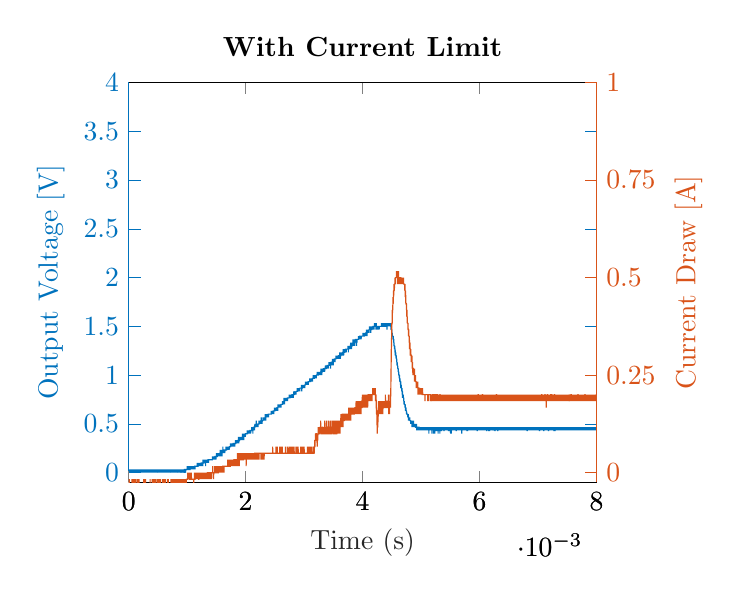
\begin{tikzpicture}

\begin{axis}[%
width=0.49\textwidth,
height=2in,
at={(0.758in,0.481in)},
scale only axis,
xmin=0,
xmax=0.008,
xlabel style={font=\color{white!15!black}},
xlabel={Time (s)},
separate axis lines,
every outer y axis line/.append style={mycolor1},
every y tick label/.append style={font=\color{mycolor1}},
every y tick/.append style={mycolor1},
ymin=-0.1,
ymax=4,
ytick={  0, 0.5,   1, 1.5,   2, 2.5,   3, 3.5,   4},
ylabel style={font=\color{mycolor1}},
ylabel={Output Voltage [V]},
axis background/.style={fill=white},
title style={font=\bfseries},
title={With Current Limit}
]
\addplot [color=mycolor1, forget plot]
  table[row sep=crcr]{%
-3.05000000810907e-08	0.0333333\\
9.69500000058687e-07	0\\
1.16949999995342e-06	0.0333333\\
1.36950000007019e-06	0\\
1.76950000008169e-06	0.0333333\\
2.5695000001047e-06	0\\
2.76949999999943e-06	0.0333333\\
2.96949999989415e-06	0\\
3.16950000001093e-06	0.0333333\\
3.76949999991716e-06	0\\
3.96950000003393e-06	0.0333333\\
5.36949999996317e-06	0\\
5.76949999997467e-06	0.0333333\\
5.96950000009144e-06	0\\
6.36950000010295e-06	0.0333333\\
6.7694999998924e-06	0\\
6.96950000000918e-06	0.0333333\\
7.16949999990391e-06	0\\
7.36950000002068e-06	0.0333333\\
8.36949999993841e-06	0\\
8.56950000005519e-06	0.0333333\\
8.96950000006669e-06	0\\
9.16949999996142e-06	0.0333333\\
1.13694999999137e-05	0\\
1.19695000000419e-05	0.0333333\\
1.21694999999367e-05	0\\
1.23695000000534e-05	0.0333333\\
1.27695000000649e-05	0\\
1.29694999999597e-05	0.0333333\\
1.37694999999827e-05	0\\
1.39695000000994e-05	0.0333333\\
1.55694999999234e-05	0\\
1.59694999999349e-05	0.0333333\\
1.65695000000632e-05	0\\
1.71694999999694e-05	0.0333333\\
1.77695000000977e-05	0\\
1.81695000001092e-05	0.0333333\\
1.85694999998987e-05	0\\
1.87695000000154e-05	0.0333333\\
1.91695000000269e-05	0\\
1.93694999999217e-05	0.0333333\\
1.97694999999332e-05	0\\
1.99695000000499e-05	0.0333333\\
2.07695000000729e-05	0\\
2.09694999999677e-05	0.0333333\\
2.21695000000022e-05	0\\
2.23694999998969e-05	0.0333333\\
2.29695000000252e-05	0\\
2.33695000000367e-05	0.0333333\\
2.35694999999314e-05	0\\
2.37695000000482e-05	0.0333333\\
2.61694999998952e-05	0\\
2.73694999999297e-05	0.0333333\\
2.75695000000464e-05	0\\
2.77694999999412e-05	0.0333333\\
2.79695000000579e-05	0\\
2.81694999999527e-05	0.0333333\\
2.87695000000809e-05	0\\
2.91695000000924e-05	0.0333333\\
2.93694999999872e-05	0\\
3.01695000000102e-05	0.0333333\\
3.03694999999049e-05	0\\
3.05695000000217e-05	0.0333333\\
3.07694999999164e-05	0\\
3.11694999999279e-05	0.0333333\\
3.13695000000447e-05	0\\
3.17695000000562e-05	0.0333333\\
3.19694999999509e-05	0\\
3.23694999999624e-05	0.0333333\\
3.27694999999739e-05	0\\
3.29695000000907e-05	0.0333333\\
3.45694999999147e-05	0\\
3.51695000000429e-05	0.0333333\\
3.59695000000659e-05	0\\
3.61694999999607e-05	0.0333333\\
3.65694999999722e-05	0\\
3.67695000000889e-05	0.0333333\\
3.73694999999952e-05	0\\
3.77695000000067e-05	0.0333333\\
3.83694999999129e-05	0\\
3.85695000000297e-05	0.0333333\\
3.97695000000642e-05	0\\
3.99694999999589e-05	0.0333333\\
4.07694999999819e-05	0\\
4.09695000000987e-05	0.0333333\\
4.17694999998997e-05	0\\
4.19695000000164e-05	0.0333333\\
4.21694999999112e-05	0\\
4.25694999999227e-05	0.0333333\\
4.33694999999457e-05	0\\
4.37694999999572e-05	0.0333333\\
4.41694999999687e-05	0\\
4.45694999999802e-05	0.0333333\\
4.61695000000262e-05	0\\
4.63694999999209e-05	0.0333333\\
4.77695000000722e-05	0\\
4.79694999999669e-05	0.0333333\\
4.83694999999784e-05	0\\
4.95695000000129e-05	0.0333333\\
4.97694999999077e-05	0\\
5.01694999999192e-05	0.0333333\\
5.11695000000589e-05	0\\
5.17694999999652e-05	0.0333333\\
5.21694999999767e-05	0\\
5.25694999999882e-05	0.0333333\\
5.27695000001049e-05	0\\
5.29694999999997e-05	0.0333333\\
5.33695000000112e-05	0\\
5.37695000000227e-05	0.0333333\\
5.39694999999174e-05	0\\
5.43694999999289e-05	0.0333333\\
5.47694999999404e-05	0\\
5.49695000000572e-05	0.0333333\\
5.63694999999864e-05	0\\
5.69694999998926e-05	0.0333333\\
5.73694999999041e-05	0\\
5.75695000000209e-05	0.0333333\\
5.79695000000324e-05	0\\
5.81694999999272e-05	0.0333333\\
5.83695000000439e-05	0\\
5.85694999999387e-05	0.0333333\\
5.93694999999617e-05	0\\
5.95695000000784e-05	0.0333333\\
5.97694999999732e-05	0\\
6.03695000001014e-05	0.0333333\\
6.05694999999962e-05	0\\
6.07694999998909e-05	0.0333333\\
6.09695000000077e-05	0\\
6.17695000000307e-05	0.0333333\\
6.19694999999254e-05	0\\
6.23694999999369e-05	0.0333333\\
6.25695000000537e-05	0\\
6.27694999999484e-05	0.0333333\\
6.39694999999829e-05	0\\
6.43694999999944e-05	0.0333333\\
6.45695000001112e-05	0\\
6.47695000000059e-05	0.0333333\\
6.49694999999006e-05	0\\
6.55695000000289e-05	0.0333333\\
6.57694999999237e-05	0\\
6.59695000000404e-05	0.0333333\\
6.61694999999352e-05	0\\
6.65694999999467e-05	0.0333333\\
6.77694999999812e-05	0\\
6.91694999999104e-05	0.0333333\\
6.95694999999219e-05	0\\
6.97695000000387e-05	0.0333333\\
7.01695000000502e-05	0\\
7.05695000000617e-05	0.0333333\\
7.07694999999564e-05	0\\
7.09695000000732e-05	0.0333333\\
7.19694999999909e-05	0\\
7.21695000001077e-05	0.0333333\\
7.45694999999547e-05	0\\
7.53694999999777e-05	0.0333333\\
7.59695000001059e-05	0\\
7.63694999998954e-05	0.0333333\\
7.67694999999069e-05	0\\
7.69695000000237e-05	0.0333333\\
7.93695000000927e-05	0\\
8.01694999998936e-05	0.0333333\\
8.05694999999051e-05	0\\
8.07695000000219e-05	0.0333333\\
8.15695000000449e-05	0\\
8.17694999999397e-05	0.0333333\\
8.25694999999627e-05	0\\
8.29694999999742e-05	0.0333333\\
8.53695000000432e-05	0\\
8.61695000000662e-05	0.0333333\\
8.65695000000777e-05	0\\
8.69695000000892e-05	0.0333333\\
8.73695000001007e-05	0\\
8.75694999999954e-05	0.0333333\\
8.83695000000184e-05	0\\
8.85694999999131e-05	0.0333333\\
8.91695000000414e-05	0\\
8.93694999999362e-05	0.0333333\\
8.97694999999477e-05	0\\
8.99695000000644e-05	0.0333333\\
9.09694999999822e-05	0\\
9.11695000000989e-05	0.0333333\\
9.15695000001104e-05	0\\
9.17695000000052e-05	0.0333333\\
9.19694999998999e-05	0\\
9.23694999999114e-05	0.0333333\\
9.29695000000397e-05	0\\
9.31694999999344e-05	0.0333333\\
9.35694999999459e-05	0\\
9.37695000000627e-05	0.0333333\\
9.47694999999804e-05	0\\
9.51694999999919e-05	0.0333333\\
9.69694999999327e-05	0\\
9.71695000000494e-05	0.0333333\\
9.93695000000017e-05	0\\
9.95694999998964e-05	0.0333333\\
0.000101969499999965	0\\
0.000102369499999977	0.0333333\\
0.000103369499999895	0\\
0.000103769499999906	0.0333333\\
0.000105169500000057	0\\
0.000105369499999952	0.0333333\\
0.000105569500000069	0\\
0.00010596950000008	0.0333333\\
0.000107169499999893	0\\
0.000107569499999904	0.0333333\\
0.000108369499999927	0\\
0.000108569500000044	0.0333333\\
0.00011016950000009	0\\
0.000110369499999985	0.0333333\\
0.000110769499999996	0\\
0.000110969499999891	0.0333333\\
0.000111169500000008	0\\
0.000111969500000031	0.0333333\\
0.000112169499999926	0\\
0.000112369500000042	0.0333333\\
0.000113569500000077	0\\
0.000113769499999972	0.0333333\\
0.000113969500000088	0\\
0.000114569499999995	0.0333333\\
0.000114969500000006	0\\
0.000115169499999901	0.0333333\\
0.000115569499999912	0\\
0.000115969499999924	0.0333333\\
0.000117169499999958	0\\
0.000117769500000087	0.0333333\\
0.000117969499999981	0\\
0.000118169500000098	0.0333333\\
0.000118369499999993	0\\
0.000118969499999899	0.0333333\\
0.000119569500000027	0\\
0.000120569499999945	0.0333333\\
0.000120769500000062	0\\
0.000121169500000073	0.0333333\\
0.000121569500000085	0\\
0.00012176949999998	0.0333333\\
0.000122169499999991	0\\
0.000122369500000108	0.0333333\\
0.000123969499999932	0\\
0.000124169500000049	0.0333333\\
0.00012456950000006	0\\
0.000125369500000083	0.0333333\\
0.000126169500000106	0\\
0.000126369500000001	0.0333333\\
0.000126769500000012	0\\
0.000126969499999907	0.0333333\\
0.000127169500000024	0\\
0.00012776949999993	0.0333333\\
0.000128969499999965	0\\
0.000129169500000081	0.0333333\\
0.000129369499999976	0\\
0.000129969500000104	0.0333333\\
0.000130169499999999	0\\
0.000130369499999894	0.0333333\\
0.000130569500000011	0\\
0.000130969500000022	0.0333333\\
0.000132369499999951	0\\
0.000132569500000068	0.0333333\\
0.000132769499999963	0\\
0.000133169499999974	0.0333333\\
0.000134369500000009	0\\
0.000134569499999904	0.0333333\\
0.00013476950000002	0\\
0.000135169500000032	0.0333333\\
0.000137569500000101	0\\
0.000137769499999996	0.0333333\\
0.00013896950000003	0\\
0.000139169499999925	0.0333333\\
0.000139569499999936	0\\
0.000139769500000053	0.0333333\\
0.000139969499999948	0\\
0.000140169500000065	0.0333333\\
0.000140769499999971	0\\
0.000140969500000088	0.0333333\\
0.000141569499999994	0\\
0.000141769500000111	0.0333333\\
0.000142369500000017	0\\
0.000142569499999912	0.0333333\\
0.000142769500000028	0\\
0.000142969499999923	0.0333333\\
0.00014316950000004	0\\
0.000143369499999935	0.0333333\\
0.000144769500000086	0\\
0.000145169500000097	0.0333333\\
0.000145769500000004	0\\
0.000145969499999898	0.0333333\\
0.000146569500000027	0\\
0.000146769499999921	0.0333333\\
0.000146969500000038	0\\
0.00014736950000005	0.0333333\\
0.000148569500000084	0\\
0.000148769499999979	0.0333333\\
0.000148969500000096	0\\
0.00014916949999999	0.0333333\\
0.000149969500000013	0\\
0.000150169499999908	0.0333333\\
0.000150369500000025	0\\
0.000150769500000036	0.0333333\\
0.000150969499999931	0\\
0.000151169500000048	0.0333333\\
0.000151369499999943	0\\
0.000151569500000059	0.0333333\\
0.000151769499999954	0\\
0.000151969500000071	0.0333333\\
0.000152569499999977	0\\
0.000152769500000094	0.0333333\\
0.000152969499999989	0\\
0.000153169500000105	0.0333333\\
0.0001533695	0\\
0.000153569499999895	0.0333333\\
0.000153769500000012	0\\
0.000153969499999906	0.0333333\\
0.000154969500000046	0\\
0.000155169499999941	0.0333333\\
0.000155369500000058	0\\
0.000155569499999952	0.0333333\\
0.000155969499999964	0\\
0.000156169500000081	0.0333333\\
0.000156569500000092	0\\
0.000156769499999987	0.0333333\\
0.000159169500000056	0\\
0.000159569500000067	0.0333333\\
0.000160569499999985	0\\
0.000161169499999891	0.0333333\\
0.000161369500000008	0\\
0.000161569499999903	0.0333333\\
0.000162969500000054	0\\
0.000163369500000066	0.0333333\\
0.000163769500000077	0\\
0.000164169500000089	0.0333333\\
0.0001645695000001	0\\
0.000164769499999995	0.0333333\\
0.000165569500000018	0\\
0.000165969500000029	0.0333333\\
0.000166169499999924	0\\
0.000167369499999959	0.0333333\\
0.000167569500000075	0\\
0.00016776949999997	0.0333333\\
0.000167969500000087	0\\
0.000168169499999982	0.0333333\\
0.000169369500000016	0\\
0.000169569499999911	0.0333333\\
0.000169969499999922	0\\
0.000170769499999945	0.0333333\\
0.000171169499999957	0\\
0.000171769500000085	0.0333333\\
0.00017196949999998	0\\
0.000172169500000097	0.0333333\\
0.000173369499999909	0\\
0.000173569500000026	0.0333333\\
0.000174169499999932	0\\
0.000174369500000049	0.0333333\\
0.000175569500000083	0\\
0.000175769499999978	0.0333333\\
0.000177769500000036	0\\
0.00017796949999993	0.0333333\\
0.000178369499999942	0\\
0.00017896950000007	0.0333333\\
0.000179369500000082	0\\
0.000179569499999976	0.0333333\\
0.000179969499999988	0\\
0.000180169500000105	0.0333333\\
0.000180569499999894	0\\
0.000180769500000011	0.0333333\\
0.000181169500000022	0\\
0.000181369499999917	0.0333333\\
0.000181769499999929	0\\
0.000181969500000045	0.0333333\\
0.00018216949999994	0\\
0.000182769500000068	0.0333333\\
0.000183769499999986	0\\
0.000184369499999892	0.0333333\\
0.000185169499999915	0\\
0.000185369500000032	0.0333333\\
0.000185969499999938	0\\
0.00018636949999995	0.0333333\\
0.000187169499999973	0\\
0.00018736950000009	0.0333333\\
0.000187569499999984	0\\
0.000187969499999996	0.0333333\\
0.000188769500000019	0\\
0.000188969499999914	0.0333333\\
0.00018916950000003	0\\
0.000189569500000042	0.0333333\\
0.00019056949999996	0\\
0.000190769500000076	0.0333333\\
0.000190969499999971	0\\
0.000191569500000099	0.0333333\\
0.0001923694999999	0\\
0.000192569500000017	0.0333333\\
0.00019336950000004	0\\
0.000193569499999935	0.0333333\\
0.000193769500000052	0\\
0.000193969499999946	0.0333333\\
0.000194769499999969	0\\
0.000194969500000086	0.0333333\\
0.000195369500000098	0\\
0.000195769500000109	0.0333333\\
0.00019656949999991	0\\
0.000196969499999922	0.0333333\\
0.000197369499999933	0\\
0.00019756950000005	0.0333333\\
0.000199569500000107	0\\
0.000199769500000002	0.0333333\\
0.000200969500000037	0\\
0.000201369500000048	0.0333333\\
0.000202569500000083	0\\
0.000202969500000094	0.0333333\\
0.000203369500000106	0\\
0.0002035695	0.0333333\\
0.000203769499999895	0\\
0.000203969500000012	0.0333333\\
0.000204169499999907	0\\
0.000204769500000035	0.0333333\\
0.000205369499999941	0\\
0.000206769500000092	0.0333333\\
0.000206969499999987	0\\
0.000207569499999893	0.0333333\\
0.000208569500000033	0\\
0.000209569499999951	0.0333333\\
0.000209969499999962	0\\
0.000210369499999974	0.0333333\\
0.000210569500000091	0\\
0.000210969500000102	0.0333333\\
0.000211169499999997	0\\
0.000211369499999892	0.0333333\\
0.000211769499999903	0\\
0.000212369500000031	0.0333333\\
0.000212569499999926	0\\
0.000212769500000043	0.0333333\\
0.000212969499999938	0\\
0.000213369499999949	0.0333333\\
0.000214169499999972	0\\
0.000214369500000089	0.0333333\\
0.000215969499999913	0\\
0.00021616950000003	0.0333333\\
0.000216369499999924	0\\
0.000216569500000041	0.0333333\\
0.000216769499999936	0\\
0.000217369500000064	0.0333333\\
0.000217569499999959	0\\
0.000217769500000076	0.0333333\\
0.00021796949999997	0\\
0.000218169500000087	0.0333333\\
0.000219169500000005	0\\
0.000219569500000016	0.0333333\\
0.000219769499999911	0\\
0.000219969500000028	0.0333333\\
0.000220169499999923	0\\
0.000220569499999934	0.0333333\\
0.000221969500000085	0\\
0.000222569499999992	0.0333333\\
0.000223169499999898	0\\
0.000223769500000026	0.0333333\\
0.000223969499999921	0\\
0.000224369499999932	0.0333333\\
0.000224569500000049	0\\
0.000224969500000061	0.0333333\\
0.000225369500000072	0\\
0.000225569499999967	0.0333333\\
0.000225769500000084	0\\
0.00022636949999999	0.0333333\\
0.000226769500000001	0\\
0.000226969499999896	0.0333333\\
0.000227569500000024	0\\
0.000227969500000036	0.0333333\\
0.000228169499999931	0\\
0.000228569499999942	0.0333333\\
0.00022916950000007	0\\
0.000229369499999965	0.0333333\\
0.000229969500000093	0\\
0.000231569499999917	0.0333333\\
0.000231969499999929	0\\
0.000232169500000046	0.0333333\\
0.00023236949999994	0\\
0.000232569500000057	0.0333333\\
0.000232769499999952	0\\
0.00023336950000008	0.0333333\\
0.000233769500000092	0\\
0.000233969499999986	0.0333333\\
0.000234569499999893	0\\
0.000234969499999904	0.0333333\\
0.000235369499999916	0\\
0.000235569500000032	0.0333333\\
0.000236169499999939	0\\
0.000236969499999962	0.0333333\\
0.000237169500000078	0\\
0.000237369499999973	0.0333333\\
0.00023756950000009	0\\
0.000237769499999985	0.0333333\\
0.000238169499999996	0\\
0.000238769499999902	0.0333333\\
0.000238969500000019	0\\
0.000239369500000031	0.0333333\\
0.000239569499999925	0\\
0.000240369499999948	0.0333333\\
0.00024076949999996	0\\
0.000241169499999971	0.0333333\\
0.000241369500000088	0\\
0.000242969499999912	0.0333333\\
0.00024356950000004	0\\
0.000243769499999935	0.0333333\\
0.000244769500000075	0\\
0.00024496949999997	0.0333333\\
0.000245169500000086	0\\
0.000245569500000098	0.0333333\\
0.000245769499999993	0\\
0.000245969500000109	0.0333333\\
0.000246169500000004	0\\
0.000246369499999899	0.0333333\\
0.000246569500000016	0\\
0.00024676949999991	0.0333333\\
0.000247169499999922	0\\
0.000247569499999933	0.0333333\\
0.00024776950000005	0\\
0.000248369499999956	0.0333333\\
0.000248769499999968	0\\
0.000250169499999897	0.0333333\\
0.00025096949999992	0\\
0.00025196950000006	0.0333333\\
0.000252769500000083	0\\
0.000253769500000001	0.0333333\\
0.000253969499999895	0\\
0.000254169500000012	0.0333333\\
0.000255369500000047	0\\
0.000255569499999941	0.0333333\\
0.000255769500000058	0\\
0.00025616950000007	0.0333333\\
0.000256569500000081	0\\
0.000256969500000093	0.0333333\\
0.000257569499999999	0\\
0.000258169499999905	0.0333333\\
0.000258569499999917	0\\
0.000258769500000033	0.0333333\\
0.000259169500000045	0\\
0.00025936949999994	0.0333333\\
0.000259569500000056	0\\
0.000259969500000068	0.0333333\\
0.000260169499999963	0\\
0.000260369500000079	0.0333333\\
0.000260569499999974	0\\
0.000260769500000091	0.0333333\\
0.000261169500000102	0\\
0.000261769500000009	0.0333333\\
0.000262569500000032	0\\
0.000262769499999926	0.0333333\\
0.000263569499999949	0\\
0.000263769500000066	0.0333333\\
0.000264169500000078	0\\
0.000264369499999972	0.0333333\\
0.000265169499999995	0\\
0.000265769499999902	0.0333333\\
0.00026636950000003	0\\
0.000266769500000041	0.0333333\\
0.000267169500000053	0\\
0.000267369499999948	0.0333333\\
0.000267569500000064	0\\
0.000267769499999959	0.0333333\\
0.000267969500000076	0\\
0.000268169499999971	0.0333333\\
0.000268569499999982	0\\
0.000268769500000099	0.0333333\\
0.000269369500000005	0\\
0.000270769499999934	0.0333333\\
0.000271569499999957	0\\
0.00027236949999998	0.0333333\\
0.000272569500000097	0\\
0.000273369499999898	0.0333333\\
0.000273969500000026	0\\
0.000274169499999921	0.0333333\\
0.000274769500000049	0\\
0.000274969499999944	0.0333333\\
0.000275169500000061	0\\
0.000275369499999956	0.0333333\\
0.000275969500000084	0\\
0.000276369500000095	0.0333333\\
0.000276769500000107	0\\
0.000277369500000013	0.0333333\\
0.000277569499999908	0\\
0.000277969499999919	0.0333333\\
0.000278769499999942	0\\
0.000278969500000059	0.0333333\\
0.000279169499999954	0\\
0.000279369500000071	0.0333333\\
0.000279769500000082	0\\
0.000279969499999977	0.0333333\\
0.000280369499999988	0\\
0.000280569500000105	0.0333333\\
0.000281369499999906	0\\
0.000281969500000034	0.0333333\\
0.000282369500000046	0\\
0.000282569499999941	0.0333333\\
0.000282769500000057	0\\
0.000283969500000092	0.0333333\\
0.000284169499999987	0\\
0.000284569499999998	0.0333333\\
0.000284769499999893	0\\
0.00028496950000001	0.0333333\\
0.000285169499999904	0\\
0.000286369499999939	0.0333333\\
0.000286569500000056	0\\
0.000287169499999962	0.0333333\\
0.00028776950000009	0\\
0.000287969499999985	0.0333333\\
0.000289369499999914	0\\
0.000289569500000031	0.0333333\\
0.000289769499999926	0\\
0.000289969500000042	0.0333333\\
0.000290169499999937	0\\
0.000290369500000054	0.0333333\\
0.000290569499999949	0\\
0.000290769500000065	0.0333333\\
0.000291169500000077	0\\
0.000291369499999972	0.0333333\\
0.000291569500000088	0\\
0.0002919695000001	0.0333333\\
0.000292769499999901	0\\
0.000292969500000018	0.0333333\\
0.000293169499999912	0\\
0.000293769500000041	0.0333333\\
0.000293969499999935	0\\
0.000294369499999947	0.0333333\\
0.000294569500000064	0\\
0.000294769499999958	0.0333333\\
0.000294969500000075	0\\
0.00029516949999997	0.0333333\\
0.000295369500000087	0\\
0.000295569499999981	0.0333333\\
0.000295769500000098	0\\
0.000295969499999993	0.0333333\\
0.00029616950000011	0\\
0.000296369500000004	0.0333333\\
0.000296569499999899	0\\
0.00029796950000005	0.0333333\\
0.000298569499999957	0\\
0.000298769500000073	0.0333333\\
0.000299169500000085	0\\
0.00029936949999998	0.0333333\\
0.000299569500000096	0\\
0.000299969500000108	0.0333333\\
0.000300369499999897	0\\
0.000300969500000026	0.0333333\\
0.000301369500000037	0\\
0.000301569499999932	0.0333333\\
0.000301769500000049	0\\
0.000301969499999943	0.0333333\\
0.00030216950000006	0\\
0.000302369499999955	0.0333333\\
0.000302569500000072	0\\
0.000302969500000083	0.0333333\\
0.000303169499999978	0\\
0.000303569499999989	0.0333333\\
0.000303769500000106	0\\
0.000304169499999896	0.0333333\\
0.000304769500000024	0\\
0.000305969500000058	0.0333333\\
0.00030636950000007	0\\
0.000306569499999965	0.0333333\\
0.000306769500000081	0\\
0.000307769499999999	0.0333333\\
0.000307969499999894	0\\
0.000308569500000022	0.0333333\\
0.000308769499999917	0\\
0.000310369499999963	0.0333333\\
0.00031056950000008	0\\
0.000311169499999986	0.0333333\\
0.000311769499999892	0\\
0.000311969500000009	0.0333333\\
0.000312169499999904	0\\
0.000312569499999915	0.0333333\\
0.000312769500000032	0\\
0.000312969499999927	0.0333333\\
0.000313169500000043	0\\
0.000314169499999961	0.0333333\\
0.000314369500000078	0\\
0.000314569499999973	0.0333333\\
0.000314769500000089	0\\
0.000315169500000101	0.0333333\\
0.00031556949999989	0\\
0.000315769500000007	0.0333333\\
0.000316169500000019	0\\
0.000316369499999913	0.0333333\\
0.000316969500000042	0\\
0.000317769500000065	0.0333333\\
0.000318169500000076	0\\
0.000319369500000111	0.0333333\\
0.000319569500000005	0\\
0.000319969500000017	0.0333333\\
0.000320169499999912	0\\
0.000321569500000063	0.0333333\\
0.000321969500000074	0\\
0.000322369500000086	0.0333333\\
0.000322569499999981	0\\
0.000322769500000097	0.0333333\\
0.000322969499999992	0\\
0.000323369500000004	0.0333333\\
0.000323569499999898	0\\
0.00032396949999991	0.0333333\\
0.000324169500000027	0\\
0.000324569500000038	0.0333333\\
0.000324769499999933	0\\
0.00032496950000005	0.0333333\\
0.000325369500000061	0\\
0.000325969499999967	0.0333333\\
0.000326369499999979	0\\
0.000326569500000096	0.0333333\\
0.000326969500000107	0\\
0.000328369500000036	0.0333333\\
0.000328569499999931	0\\
0.000328969499999943	0.0333333\\
0.000329569500000071	0\\
0.000330369500000094	0.0333333\\
0.000330569499999989	0\\
0.0003309695	0.0333333\\
0.000331369500000012	0\\
0.000331969499999918	0.0333333\\
0.000332169500000035	0\\
0.000332569500000046	0.0333333\\
0.000332969500000058	0\\
0.000333969499999975	0.0333333\\
0.000334169500000092	0\\
0.000334569500000104	0.0333333\\
0.000334769499999998	0\\
0.00033516950000001	0.0333333\\
0.000335369499999905	0\\
0.000336569499999939	0.0333333\\
0.000337169500000067	0\\
0.000337369499999962	0.0333333\\
0.000337569500000079	0\\
0.000337769499999974	0.0333333\\
0.00033796950000009	0\\
0.000338569499999997	0.0333333\\
0.000338769499999891	0\\
0.000338969500000008	0.0333333\\
0.00033936950000002	0\\
0.000339569499999914	0.0333333\\
0.000339769500000031	0\\
0.000340169500000043	0.0333333\\
0.000340369499999937	0\\
0.000340569500000054	0.0333333\\
0.000340969500000066	0\\
0.00034116949999996	0.0333333\\
0.000341369500000077	0\\
0.000341569499999972	0.0333333\\
0.0003421695000001	0\\
0.000342369499999995	0.0333333\\
0.000342769500000006	0\\
0.000342969499999901	0.0333333\\
0.000343169500000018	0\\
0.000343569500000029	0.0333333\\
0.000344169499999936	0\\
0.000344369500000052	0.0333333\\
0.000344569499999947	0\\
0.000344769500000064	0.0333333\\
0.000344969499999959	0\\
0.000345569500000087	0.0333333\\
0.000345969500000098	0\\
0.000346169499999993	0.0333333\\
0.000346969500000016	0\\
0.000347169499999911	0.0333333\\
0.000347369500000028	0\\
0.000347969499999934	0.0333333\\
0.000348169500000051	0\\
0.000348369499999945	0.0333333\\
0.000348969500000074	0\\
0.000349969499999991	0.0333333\\
0.000350169500000108	0\\
0.000350369500000003	0.0333333\\
0.000350969499999909	0\\
0.000351169500000026	0.0333333\\
0.000351369499999921	0\\
0.000352169499999944	0.0333333\\
0.00035236950000006	0\\
0.000353169500000083	0.0333333\\
0.000353569500000095	0\\
0.000354569500000013	0.0333333\\
0.000354969500000024	0\\
0.000355169499999919	0.0333333\\
0.000355369500000036	0\\
0.00035556949999993	0.0333333\\
0.000355769500000047	0\\
0.000356169500000059	0.0333333\\
0.000356369499999953	0\\
0.000356969500000082	0.0333333\\
0.000357769500000105	0\\
0.000357969499999999	0.0333333\\
0.000358169499999894	0\\
0.000358369500000011	0.0333333\\
0.000358569499999906	0\\
0.000358769500000022	0.0333333\\
0.000359169500000034	0\\
0.000360169499999952	0.0333333\\
0.000360369500000068	0\\
0.000360569499999963	0.0333333\\
0.000361369499999986	0\\
0.000361569500000103	0.0333333\\
0.000361769499999998	0\\
0.000363369500000044	0.0333333\\
0.000363569499999938	0\\
0.000363769500000055	0.0333333\\
0.000364169500000067	0\\
0.000364369499999961	0.0333333\\
0.000364569500000078	0\\
0.00036496950000009	0.0333333\\
0.000365969500000007	0\\
0.000366169499999902	0.0333333\\
0.00036676950000003	0\\
0.000366969499999925	0.0333333\\
0.000367569500000053	0\\
0.000367769499999948	0.0333333\\
0.000368569499999971	0\\
0.000369169500000099	0.0333333\\
0.000369369499999994	0\\
0.000370569500000029	0.0333333\\
0.00037096950000004	0\\
0.000371169499999935	0.0333333\\
0.000371769500000063	0\\
0.000372369499999969	0.0333333\\
0.000372769499999981	0\\
0.000373369500000109	0.0333333\\
0.00037416949999991	0\\
0.000374569499999922	0.0333333\\
0.000374969499999933	0\\
0.000375969500000073	0.0333333\\
0.000376769500000096	0\\
0.000377969499999908	0.0333333\\
0.00037836949999992	0\\
0.000378569500000037	0.0333333\\
0.000379769500000071	0\\
0.000379969499999966	0.0333333\\
0.000380169500000083	0\\
0.000380369499999977	0.0333333\\
0.000381769499999907	0\\
0.000381969500000023	0.0333333\\
0.000382169499999918	0\\
0.00038256949999993	0.0333333\\
0.000383169500000058	0\\
0.000383369499999953	0.0333333\\
0.000383769499999964	0\\
0.000384369500000092	0.0333333\\
0.000384969499999999	0\\
0.000385169499999893	0.0333333\\
0.000385569499999905	0\\
0.000385769500000022	0.0333333\\
0.000385969499999916	0\\
0.000386169500000033	0.0333333\\
0.000386569500000045	0\\
0.000386969500000056	0.0333333\\
0.000387369500000068	0\\
0.000387569499999962	0.0333333\\
0.000387769500000079	0\\
0.000387969499999974	0.0333333\\
0.000388969499999892	0\\
0.000389169500000008	0.0333333\\
0.00038956950000002	0\\
0.000390569499999938	0.0333333\\
0.000390969499999949	0\\
0.000391169500000066	0.0333333\\
0.000391369499999961	0\\
0.000391769499999972	0.0333333\\
0.000391969500000089	0\\
0.000392169499999984	0.0333333\\
0.0003923695000001	0\\
0.000392569499999995	0.0333333\\
0.00039376950000003	0\\
0.000394169500000041	0.0333333\\
0.000395369500000076	0\\
0.00039556949999997	0.0333333\\
0.000395969499999982	0\\
0.000396369499999993	0.0333333\\
0.000397169500000016	0\\
0.000397569500000028	0.0333333\\
0.000397969500000039	0\\
0.000398369500000051	0.0333333\\
0.000398769500000062	0\\
0.000398969499999957	0.0333333\\
0.000399369499999969	0\\
0.000399569500000085	0.0333333\\
0.00039976949999998	0\\
0.000400569500000003	0.0333333\\
0.000401769500000038	0\\
0.000402169500000049	0.0333333\\
0.000402369499999944	0\\
0.000402569500000061	0.0333333\\
0.000402769499999955	0\\
0.000402969500000072	0.0333333\\
0.000403369500000084	0\\
0.000403569499999978	0.0333333\\
0.00040396949999999	0\\
0.000404969499999908	0.0333333\\
0.000405369499999919	0\\
0.000405769499999931	0.0333333\\
0.000406169499999942	0\\
0.000406369500000059	0.0333333\\
0.000407569500000093	0\\
0.0004081695	0.0333333\\
0.000408369499999894	0\\
0.000408969500000023	0.0333333\\
0.000409169499999917	0\\
0.000409769500000046	0.0333333\\
0.000410369499999952	0\\
0.00041096950000008	0.0333333\\
0.000411369500000092	0\\
0.000411769500000103	0.0333333\\
0.000413369499999927	0\\
0.00041416949999995	0.0333333\\
0.000414569499999962	0\\
0.000414969499999973	0.0333333\\
0.000416569500000019	0\\
0.000416769499999914	0.0333333\\
0.000416969500000031	0\\
0.000417169499999925	0.0333333\\
0.000417369500000042	0\\
0.000417569499999937	0.0333333\\
0.000417969499999948	0\\
0.000418569500000077	0.0333333\\
0.000418769499999971	0\\
0.000419169499999983	0.0333333\\
0.000419769500000111	0\\
0.000419969500000006	0.0333333\\
0.000420169499999901	0\\
0.000420369500000017	0.0333333\\
0.000420569499999912	0\\
0.000420769500000029	0.0333333\\
0.000420969499999924	0\\
0.000421769499999947	0.0333333\\
0.000422169499999958	0\\
0.000422369500000075	0.0333333\\
0.00042256949999997	0\\
0.000422969499999981	0.0333333\\
0.00042436949999991	0\\
0.000424969500000039	0.0333333\\
0.000425569499999945	0\\
0.000426569500000085	0.0333333\\
0.000426969500000096	0\\
0.000427769499999897	0.0333333\\
0.000429169500000048	0\\
0.000429369499999943	0.0333333\\
0.000430169499999966	0\\
0.000430369500000083	0.0333333\\
0.000430569499999978	0\\
0.000430769500000094	0.0333333\\
0.000431369500000001	0\\
0.000431969499999907	0.0333333\\
0.000432169500000024	0\\
0.000433169499999941	0.0333333\\
0.000433569499999953	0\\
0.00043376950000007	0.0333333\\
0.000433969499999964	0\\
0.000434569500000093	0.0333333\\
0.000434769499999987	0\\
0.000435169499999999	0.0333333\\
0.000435969500000022	0\\
0.000436169499999917	0.0333333\\
0.000436569499999928	0\\
0.000437569500000068	0.0333333\\
0.000437769499999963	0\\
0.000437969500000079	0.0333333\\
0.000438569499999986	0\\
0.000438769500000102	0.0333333\\
0.000439369500000009	0\\
0.000439569499999903	0.0333333\\
0.000440169500000032	0\\
0.000441169499999949	0.0333333\\
0.000441369500000066	0\\
0.000441769500000078	0.0333333\\
0.000441969499999972	0\\
0.000442169500000089	0.0333333\\
0.000442369499999984	0\\
0.000442769499999995	0.0333333\\
0.00044296949999989	0\\
0.000443169500000007	0.0333333\\
0.000443369499999902	0\\
0.000443569500000018	0.0333333\\
0.000444169499999925	0\\
0.000444569499999936	0.0333333\\
0.000444769500000053	0\\
0.000445169500000064	0.0333333\\
0.000446169499999982	0\\
0.000446569499999994	0.0333333\\
0.000446969500000005	0\\
0.0004471694999999	0.0333333\\
0.000447369500000017	0\\
0.000447569499999911	0.0333333\\
0.000447769500000028	0\\
0.00044816950000004	0.0333333\\
0.000449369500000074	0\\
0.000449569499999969	0.0333333\\
0.000450169500000097	0\\
0.000450369499999992	0.0333333\\
0.000450569500000109	0\\
0.000450769500000003	0.0333333\\
0.000450969499999898	0\\
0.000451169500000015	0.0333333\\
0.000451969500000038	0\\
0.000452169499999933	0.0333333\\
0.000452369500000049	0\\
0.000453369499999967	0.0333333\\
0.000453569500000084	0\\
0.00045416949999999	0.0333333\\
0.000454569500000002	0\\
0.000454769499999896	0.0333333\\
0.000455169499999908	0\\
0.000455569499999919	0.0333333\\
0.000457369500000082	0\\
0.000457969499999988	0.0333333\\
0.000458569499999895	0\\
0.000458769500000011	0.0333333\\
0.000458969499999906	0\\
0.000459769499999929	0.0333333\\
0.000459969500000046	0\\
0.000460169499999941	0.0333333\\
0.000460569499999952	0\\
0.000461569500000092	0.0333333\\
0.000461969500000103	0\\
0.000462169499999998	0.0333333\\
0.000462369499999893	0\\
0.000462769499999904	0.0333333\\
0.000463169499999916	0\\
0.000463769500000044	0.0333333\\
0.000463969499999939	0\\
0.000465569499999985	0.0333333\\
0.000466569499999903	0\\
0.000466969499999914	0.0333333\\
0.000467769499999937	0\\
0.000467969500000054	0.0333333\\
0.000468769500000077	0\\
0.000468969499999972	0.0333333\\
0.0004695695000001	0\\
0.000469769499999995	0.0333333\\
0.000470169500000006	0\\
0.000470569500000018	0.0333333\\
0.000470769499999912	0\\
0.000471369500000041	0.0333333\\
0.000471569499999935	0\\
0.000472169500000064	0.0333333\\
0.00047276949999997	0\\
0.000473169499999981	0.0333333\\
0.000473369500000098	0\\
0.000473569499999993	0.0333333\\
0.000474369500000016	0\\
0.000474969499999922	0.0333333\\
0.000475169500000039	0\\
0.000475369499999934	0.0333333\\
0.00047556950000005	0\\
0.000475969500000062	0.0333333\\
0.000476369500000073	0\\
0.000476569499999968	0.0333333\\
0.000476769500000085	0\\
0.000477169500000096	0.0333333\\
0.000477369499999991	0\\
0.000477969499999897	0.0333333\\
0.000478969500000037	0\\
0.000479569499999943	0.0333333\\
0.000479969499999955	0\\
0.000480369499999966	0.0333333\\
0.000481369500000106	0\\
0.000482169499999907	0.0333333\\
0.00048296949999993	0\\
0.000483769499999953	0.0333333\\
0.00048396950000007	0\\
0.000484169499999965	0.0333333\\
0.000484769500000093	0\\
0.000484969499999988	0.0333333\\
0.000485169500000104	0\\
0.000485569499999894	0.0333333\\
0.000485969499999905	0\\
0.000486169500000022	0.0333333\\
0.000486569500000034	0\\
0.000486769499999928	0.0333333\\
0.000486969500000045	0\\
0.00048716949999994	0.0333333\\
0.000487369500000057	0\\
0.000487569499999951	0.0333333\\
0.00048816950000008	0\\
0.000488569500000091	0.0333333\\
0.000489369499999892	0\\
0.000489769499999904	0.0333333\\
0.000490169499999915	0\\
0.000490369500000032	0.0333333\\
0.000490569499999927	0\\
0.000491969500000078	0.0333333\\
0.000492169499999973	0\\
0.000492569499999984	0.0333333\\
0.000492769500000101	0\\
0.00049316949999989	0.0333333\\
0.000493369500000007	0\\
0.000493769500000019	0.0333333\\
0.000495169499999948	0\\
0.000495569499999959	0.0333333\\
0.000496369499999982	0\\
0.000496569500000099	0.0333333\\
0.000498969499999946	0\\
0.000500169499999981	0.0333333\\
0.000500969500000004	0\\
0.00050156949999991	0.0333333\\
0.000501769500000027	0\\
0.000501969499999921	0.0333333\\
0.000502169500000038	0\\
0.00050256950000005	0.0333333\\
0.000503569499999967	0\\
0.000504169500000096	0.0333333\\
0.00050436949999999	0\\
0.000504769500000002	0.0333333\\
0.000504969499999897	0\\
0.000505369499999908	0.0333333\\
0.000505569500000025	0\\
0.000506369500000048	0.0333333\\
0.000506569499999943	0\\
0.000506769500000059	0.0333333\\
0.000507369499999966	0\\
0.000507569500000082	0.0333333\\
0.000508369500000105	0\\
0.0005085695	0.0333333\\
0.000509169499999906	0\\
0.000509769500000035	0.0333333\\
0.000509969499999929	0\\
0.000510169500000046	0.0333333\\
0.000511569499999975	0\\
0.000511769500000092	0.0333333\\
0.000511969499999987	0\\
0.000512569499999893	0.0333333\\
0.000513169500000021	0\\
0.000513369499999916	0.0333333\\
0.000513769499999928	0\\
0.000513969500000044	0.0333333\\
0.000514969499999962	0\\
0.000515169500000079	0.0333333\\
0.000515769499999985	0\\
0.000515969500000102	0.0333333\\
0.00051696950000002	0\\
0.000517169499999914	0.0333333\\
0.000518369499999949	0\\
0.000519169499999972	0.0333333\\
0.000519569499999983	0\\
0.000519969499999995	0.0333333\\
0.000520569499999901	0\\
0.000520769500000018	0.0333333\\
0.000521169500000029	0\\
0.000521369499999924	0.0333333\\
0.000521769499999936	0\\
0.000521969500000052	0.0333333\\
0.000522369500000064	0\\
0.000522569499999959	0.0333333\\
0.000522769500000075	0\\
0.00052296949999997	0.0333333\\
0.000523369499999982	0\\
0.000523769499999993	0.0333333\\
0.00052396950000011	0\\
0.000524769499999911	0.0333333\\
0.000525169499999922	0\\
0.000525769500000051	0.0333333\\
0.000526169500000062	0\\
0.000526569500000074	0.0333333\\
0.000526769499999968	0\\
0.000527569499999991	0.0333333\\
0.000528169499999898	0\\
0.000528969499999921	0.0333333\\
0.000529169500000037	0\\
0.000529769499999944	0.0333333\\
0.00052996950000006	0\\
0.000530169499999955	0.0333333\\
0.000530369500000072	0\\
0.000530569499999967	0.0333333\\
0.000531169500000095	0\\
0.000531569500000106	0.0333333\\
0.000532169500000013	0\\
0.000532769499999919	0.0333333\\
0.000532969500000036	0\\
0.00053316949999993	0.0333333\\
0.000533769500000059	0\\
0.000534569500000082	0.0333333\\
0.000534969500000093	0\\
0.000535569499999999	0.0333333\\
0.000536169499999906	0\\
0.000536369500000022	0.0333333\\
0.000536569499999917	0\\
0.000536769500000034	0.0333333\\
0.000536969499999929	0\\
0.000537169500000045	0.0333333\\
0.000537569500000057	0\\
0.000538169499999963	0.0333333\\
0.00053836950000008	0\\
0.000539369499999998	0.0333333\\
0.000539569499999892	0\\
0.000540969500000044	0.0333333\\
0.000541169499999938	0\\
0.00054156949999995	0.0333333\\
0.000541769500000067	0\\
0.00054256950000009	0.0333333\\
0.000542769499999984	0\\
0.000542969500000101	0.0333333\\
0.000543169499999996	0\\
0.000543769499999902	0.0333333\\
0.000543969500000019	0\\
0.000544769500000042	0.0333333\\
0.000544969499999937	0\\
0.000545169500000053	0.0333333\\
0.000545369499999948	0\\
0.000545569500000065	0.0333333\\
0.00054576949999996	0\\
0.000546569499999983	0.0333333\\
0.000546769500000099	0\\
0.000546969499999994	0.0333333\\
0.000547369500000006	0\\
0.000547769500000017	0.0333333\\
0.00054856950000004	0\\
0.000549169499999946	0.0333333\\
0.000549969499999969	0\\
0.000550169500000086	0.0333333\\
0.000550969500000109	0\\
0.000551169500000004	0.0333333\\
0.000551369499999899	0\\
0.00055176949999991	0.0333333\\
0.000551969500000027	0\\
0.000552569499999933	0.0333333\\
0.00055276950000005	0\\
0.000552969499999945	0.0333333\\
0.000554169499999979	0\\
0.000554569499999991	0.0333333\\
0.000555169499999897	0\\
0.000555369500000014	0.0333333\\
0.000555569499999908	0\\
0.000555769500000025	0.0333333\\
0.000556169500000037	0\\
0.000556369499999931	0.0333333\\
0.000556769499999943	0\\
0.00055696950000006	0.0333333\\
0.000557569499999966	0\\
0.000557769500000083	0.0333333\\
0.000558169500000094	0\\
0.000558369499999989	0.0333333\\
0.0005587695	0\\
0.000558969499999895	0.0333333\\
0.000559169500000012	0\\
0.000559369499999907	0.0333333\\
0.000559569500000023	0\\
0.00056016949999993	0.0333333\\
0.000560369500000046	0\\
0.000560769500000058	0.0333333\\
0.000561369499999964	0\\
0.000561769499999976	0.0333333\\
0.000561969500000092	0\\
0.000562369500000104	0.0333333\\
0.000562569499999999	0\\
0.000562769499999893	0.0333333\\
0.00056296950000001	0\\
0.000563369500000022	0.0333333\\
0.000563569499999916	0\\
0.000564169500000045	0.0333333\\
0.000564369499999939	0\\
0.000564769499999951	0.0333333\\
0.000564969500000068	0\\
0.000565569499999974	0.0333333\\
0.000565769500000091	0\\
0.000565969499999985	0.0333333\\
0.000566369499999997	0\\
0.000566569499999892	0.0333333\\
0.000566769500000008	0\\
0.00056716950000002	0.0333333\\
0.000568169499999938	0\\
0.000568569499999949	0.0333333\\
0.000568769500000066	0\\
0.000568969499999961	0.0333333\\
0.000569169500000077	0\\
0.000569769499999984	0.0333333\\
0.000570169499999995	0\\
0.00057036949999989	0.0333333\\
0.000570569500000007	0\\
0.000570769499999901	0.0333333\\
0.000570969500000018	0\\
0.00057136950000003	0.0333333\\
0.000571569499999924	0\\
0.000571769500000041	0.0333333\\
0.000572169500000053	0\\
0.000572569500000064	0.0333333\\
0.000572769499999959	0\\
0.000572969500000076	0.0333333\\
0.000573369500000087	0\\
0.0005745694999999	0.0333333\\
0.000574969499999911	0\\
0.000576169499999946	0.0333333\\
0.000576369500000062	0\\
0.000576569499999957	0.0333333\\
0.000576969499999969	0\\
0.000577169500000085	0.0333333\\
0.00057736949999998	0\\
0.000577569500000097	0.0333333\\
0.000577969500000108	0\\
0.000578169500000003	0.0333333\\
0.000578369499999898	0\\
0.000578769499999909	0.0333333\\
0.000578969500000026	0\\
0.000579169499999921	0.0333333\\
0.000580169500000061	0\\
0.000580369499999955	0.0333333\\
0.000580569500000072	0\\
0.000580969500000084	0.0333333\\
0.000581369500000095	0\\
0.00058156949999999	0.0333333\\
0.000582569499999908	0\\
0.000582969499999919	0.0333333\\
0.000583169500000036	0\\
0.000583369499999931	0.0333333\\
0.000583769499999942	0\\
0.000585569500000105	0.0333333\\
0.0005857695	0\\
0.000585969499999894	0.0333333\\
0.000586169500000011	0\\
0.000586569500000023	0.0333333\\
0.000586769499999917	0\\
0.000586969500000034	0.0333333\\
0.000587169499999929	0\\
0.000587369500000046	0.0333333\\
0.000587769500000057	0\\
0.000587969499999952	0.0333333\\
0.000588169500000069	0\\
0.000588969500000092	0.0333333\\
0.000589169499999986	0\\
0.000590169499999904	0.0333333\\
0.000590569499999916	0\\
0.000590969499999927	0.0333333\\
0.000591169500000044	0\\
0.00059176949999995	0.0333333\\
0.000591969500000067	0\\
0.000592169499999962	0.0333333\\
0.000592369500000078	0\\
0.00059276950000009	0.0333333\\
0.000593369499999996	0\\
0.000593569499999891	0.0333333\\
0.000593769500000008	0\\
0.000593969499999902	0.0333333\\
0.000594169500000019	0\\
0.000594369499999914	0.0333333\\
0.00059596949999996	0\\
0.000596569500000088	0.0333333\\
0.000596769499999983	0\\
0.000597369500000111	0.0333333\\
0.000597569500000006	0\\
0.000597969500000017	0.0333333\\
0.000598169499999912	0\\
0.000598369500000029	0.0333333\\
0.000598569499999924	0\\
0.00059876950000004	0.0333333\\
0.000598969499999935	0\\
0.000599169500000052	0.0333333\\
0.000599369499999947	0\\
0.00060016949999997	0.0333333\\
0.000600769500000098	0\\
0.000600969499999993	0.0333333\\
0.000601769500000016	0\\
0.000602169500000027	0.0333333\\
0.000602569500000039	0\\
0.00060296950000005	0.0333333\\
0.000603169499999945	0\\
0.000603569499999956	0.0333333\\
0.000603969499999968	0\\
0.000604169500000085	0.0333333\\
0.000604369499999979	0\\
0.000604569500000096	0.0333333\\
0.000604769499999991	0\\
0.000605969500000025	0.0333333\\
0.00060616949999992	0\\
0.000606369500000037	0.0333333\\
0.000606769500000048	0\\
0.000606969499999943	0.0333333\\
0.000607769499999966	0\\
0.000608569499999989	0.0333333\\
0.000608769500000106	0\\
0.000609169499999895	0.0333333\\
0.000609369500000012	0\\
0.000610969500000058	0.0333333\\
0.000611169499999953	0\\
0.00061136950000007	0.0333333\\
0.000611769500000081	0\\
0.000612169500000093	0.0333333\\
0.000612369499999987	0\\
0.000612569500000104	0.0333333\\
0.000612769499999999	0\\
0.000613769499999917	0.0333333\\
0.000614369500000045	0\\
0.000614769500000056	0.0333333\\
0.000615569500000079	0\\
0.000616369500000102	0.0333333\\
0.000616769499999892	0\\
0.000616969500000009	0.0333333\\
0.000617169499999903	0\\
0.000617769500000032	0.0333333\\
0.000618569500000055	0\\
0.000619969499999984	0.0333333\\
0.000620169500000101	0\\
0.000620769500000007	0.0333333\\
0.000620969499999902	0\\
0.000621169500000018	0.0333333\\
0.00062156950000003	0\\
0.000621769499999925	0.0333333\\
0.000621969500000041	0\\
0.000622369500000053	0.0333333\\
0.000622569499999948	0\\
0.000623169500000076	0.0333333\\
0.000623769499999982	0\\
0.000623969500000099	0.0333333\\
0.000624569500000005	0\\
0.0006247694999999	0.0333333\\
0.000625169499999911	0\\
0.000625369500000028	0.0333333\\
0.000625969499999934	0\\
0.000626369499999946	0.0333333\\
0.000626569500000063	0\\
0.000626969500000074	0.0333333\\
0.000627969499999992	0\\
0.000628169500000109	0.0333333\\
0.000628369500000003	0\\
0.000628569499999898	0.0333333\\
0.000628769500000015	0\\
0.000629569500000038	0.0333333\\
0.000630169499999944	0\\
0.000630369500000061	0.0333333\\
0.000630969499999967	0\\
0.000631169500000084	0.0333333\\
0.00063176949999999	0\\
0.000631969500000107	0.0333333\\
0.000632569500000013	0\\
0.000633369500000036	0.0333333\\
0.000633969499999942	0\\
0.000634169500000059	0.0333333\\
0.000634969500000082	0\\
0.000635369500000094	0.0333333\\
0.000635569499999988	0\\
0.000635769500000105	0.0333333\\
0.0006359695	0\\
0.000636169499999895	0.0333333\\
0.000636969499999918	0\\
0.000637169500000034	0.0333333\\
0.000637369499999929	0\\
0.000637569500000046	0.0333333\\
0.000637969500000057	0\\
0.000638369500000069	0.0333333\\
0.000638569499999964	0\\
0.000638969499999975	0.0333333\\
0.000639369499999987	0\\
0.000639569500000103	0.0333333\\
0.000639769499999998	0\\
0.000639969499999893	0.0333333\\
0.00064016950000001	0\\
0.000640569500000021	0.0333333\\
0.000640769499999916	0\\
0.000641169499999927	0.0333333\\
0.000641369500000044	0\\
0.000641569499999939	0.0333333\\
0.000642169500000067	0\\
0.000642569500000079	0.0333333\\
0.000643169499999985	0\\
0.000643569499999996	0.0333333\\
0.000643769499999891	0\\
0.000643969500000008	0.0333333\\
0.000644169499999903	0\\
0.000644969499999926	0.0333333\\
0.000645369499999937	0\\
0.000645569500000054	0.0333333\\
0.000645969500000065	0\\
0.000646769500000088	0.0333333\\
0.000646969499999983	0\\
0.0006471695000001	0.0333333\\
0.000647369499999995	0\\
0.000647969499999901	0.0333333\\
0.000648369499999912	0\\
0.000648769499999924	0.0333333\\
0.000648969500000041	0\\
0.000649369500000052	0.0333333\\
0.000649569499999947	0\\
0.000650769499999981	0.0333333\\
0.000651769499999899	0\\
0.000652169499999911	0.0333333\\
0.000652769500000039	0\\
0.000652969499999934	0.0333333\\
0.000653569500000062	0\\
0.000653769499999957	0.0333333\\
0.000654369500000085	0\\
0.00065456949999998	0.0333333\\
0.000654969499999991	0\\
0.000655369500000003	0.0333333\\
0.000655569499999897	0\\
0.000656169500000026	0.0333333\\
0.00065636949999992	0\\
0.000656769499999932	0.0333333\\
0.000656969500000049	0\\
0.000657569499999955	0.0333333\\
0.000657969499999966	0\\
0.000658369499999978	0.0333333\\
0.000658769499999989	0\\
0.000658969500000106	0.0333333\\
0.000660369500000035	0\\
0.00066056949999993	0.0333333\\
0.000661969500000081	0\\
0.000663169499999894	0.0333333\\
0.000663369500000011	0\\
0.000663769500000022	0.0333333\\
0.000664169500000034	0\\
0.000664369499999928	0.0333333\\
0.000665169499999951	0\\
0.000665569499999963	0.0333333\\
0.000665969499999974	0\\
0.000666169500000091	0.0333333\\
0.000666369499999986	0\\
0.000666569500000103	0.0333333\\
0.000666769499999997	0\\
0.000667169500000009	0.0333333\\
0.00066756950000002	0\\
0.000667969500000032	0.0333333\\
0.000668169499999927	0\\
0.000668369500000043	0.0333333\\
0.000668569499999938	0\\
0.000668769500000055	0.0333333\\
0.00066896949999995	0\\
0.000669169500000066	0.0333333\\
0.000669369499999961	0\\
0.000669769499999973	0.0333333\\
0.000669969500000089	0\\
0.000670169499999984	0.0333333\\
0.000670969500000007	0\\
0.000671169499999902	0.0333333\\
0.000671369500000019	0\\
0.000672169500000042	0.0333333\\
0.000672569500000053	0\\
0.000672969500000065	0.0333333\\
0.000674169500000099	0\\
0.000675169500000017	0.0333333\\
0.000675569500000028	0\\
0.00067596950000004	0.0333333\\
0.000676169499999935	0\\
0.000676369500000051	0.0333333\\
0.000676769500000063	0\\
0.000676969499999958	0.0333333\\
0.000677169500000074	0\\
0.000677769499999981	0.0333333\\
0.000677969500000097	0\\
0.000678769499999898	0.0333333\\
0.000678969500000015	0\\
0.00067916949999991	0.0333333\\
0.000679369500000027	0\\
0.000679569499999921	0.0333333\\
0.00068016950000005	0\\
0.000680369499999944	0.0333333\\
0.000680569500000061	0\\
0.000680969500000073	0.0333333\\
0.000681169499999967	0\\
0.000682169500000107	0.0333333\\
0.000682369500000002	0\\
0.000683569500000036	0.0333333\\
0.000683769499999931	0\\
0.000684169499999943	0.0333333\\
0.000684369500000059	0\\
0.000684769500000071	0.0333333\\
0.000684969499999966	0\\
0.000685769499999989	0.0333333\\
0.000685969500000105	0\\
0.0006861695	0.0333333\\
0.000686369499999895	0\\
0.000686569500000012	0.0333333\\
0.000686769499999906	0\\
0.000686969500000023	0.0333333\\
0.000687169499999918	0\\
0.000687569499999929	0.0333333\\
0.000688769499999964	0\\
0.000689369500000092	0.0333333\\
0.000689969499999998	0\\
0.000690169499999893	0.0333333\\
0.00069036950000001	0\\
0.000690569499999905	0.0333333\\
0.000690769500000021	0\\
0.000690969499999916	0.0333333\\
0.000691369499999928	0\\
0.000691769499999939	0.0333333\\
0.000691969500000056	0\\
0.000692569499999962	0.0333333\\
0.000692769500000079	0\\
0.000692969499999974	0.0333333\\
0.00069316950000009	0\\
0.000693969499999891	0.0333333\\
0.000694169500000008	0\\
0.00069456950000002	0.0333333\\
0.000695569499999937	0\\
0.000695769500000054	0.0333333\\
0.000695969499999949	0\\
0.000696169500000066	0.0333333\\
0.000696969500000089	0\\
0.0006973695000001	0.0333333\\
0.000697569499999995	0\\
0.000698169499999901	0.0333333\\
0.000698769500000029	0\\
0.000698969499999924	0.0333333\\
0.000699169500000041	0\\
0.000699369499999936	0.0333333\\
0.000699569500000052	0\\
0.000699769499999947	0.0333333\\
0.000700369500000075	0\\
0.00070056949999997	0.0333333\\
0.000700969499999982	0\\
0.000701169500000098	0.0333333\\
0.00070156950000011	0\\
0.000701769500000005	0.0333333\\
0.000701969499999899	0\\
0.000702369499999911	0.0333333\\
0.000702969500000039	0\\
0.000703169499999934	0.0333333\\
0.000703769500000062	0\\
0.000704169500000074	0.0333333\\
0.000705969500000014	0\\
0.000706169499999909	0.0333333\\
0.000707169500000049	0\\
0.000707369499999944	0.0333333\\
0.00070756950000006	0\\
0.000707969500000072	0.0333333\\
0.000708169499999967	0\\
0.000708369500000083	0.0333333\\
0.000709969499999907	0\\
0.000710169500000024	0.0333333\\
0.000711369500000059	0\\
0.000711969499999965	0.0333333\\
0.000712169500000082	0\\
0.000713369499999894	0.0333333\\
0.000714169499999917	0\\
0.000714769500000045	0.0333333\\
0.00071496949999994	0\\
0.000716569499999986	0.0333333\\
0.000717169499999892	0\\
0.000717369500000009	0.0333333\\
0.000718169500000032	0\\
0.000718769499999938	0.0333333\\
0.000718969500000055	0\\
0.00071916949999995	0.0333333\\
0.000719769500000078	0\\
0.000719969499999973	0.0333333\\
0.000720569500000101	0\\
0.000720769499999996	0.0333333\\
0.000720969499999891	0\\
0.000721169500000007	0.0333333\\
0.000721369499999902	0\\
0.000721769499999914	0.0333333\\
0.00072196950000003	0\\
0.000722169499999925	0.0333333\\
0.000722769500000053	0\\
0.000723169500000065	0.0333333\\
0.000724169499999983	0\\
0.000724369500000099	0.0333333\\
0.000724769500000111	0\\
0.0007251694999999	0.0333333\\
0.000725569499999912	0\\
0.000725769500000029	0.0333333\\
0.000726369499999935	0\\
0.000726969500000063	0.0333333\\
0.000727169499999958	0\\
0.000728169500000098	0.0333333\\
0.000728569500000109	0\\
0.000728769500000004	0.0333333\\
0.000731169500000073	0\\
0.000731769499999979	0.0333333\\
0.000732169499999991	0\\
0.000732369500000107	0.0333333\\
0.000732569500000002	0\\
0.000732769499999897	0.0333333\\
0.00073356949999992	0\\
0.000733969499999931	0.0333333\\
0.00073456950000006	0\\
0.000734969500000071	0.0333333\\
0.000735169499999966	0\\
0.000735569499999977	0.0333333\\
0.000735769500000094	0\\
0.000736169500000106	0.0333333\\
0.0007363695	0\\
0.000736569499999895	0.0333333\\
0.000737369499999918	0\\
0.000737969500000046	0.0333333\\
0.000738169499999941	0\\
0.000738569499999953	0.0333333\\
0.000739569500000092	0\\
0.000739769499999987	0.0333333\\
0.000739969500000104	0\\
0.000740169499999999	0.0333333\\
0.000740369499999893	0\\
0.00074056950000001	0.0333333\\
0.000741369500000033	0\\
0.000741569499999928	0.0333333\\
0.000741769500000045	0\\
0.000742169500000056	0.0333333\\
0.000742769499999962	0\\
0.000743169499999974	0.0333333\\
0.000743569499999985	0\\
0.000744169499999892	0.0333333\\
0.00074476950000002	0\\
0.000744969499999915	0.0333333\\
0.000745169500000031	0\\
0.000745369499999926	0.0333333\\
0.000746369500000066	0\\
0.000746769500000077	0.0333333\\
0.000746969499999972	0\\
0.00074796949999989	0.0333333\\
0.000748169500000007	0\\
0.000748369499999901	0.0333333\\
0.000748569500000018	0\\
0.000748769499999913	0.0333333\\
0.00074896950000003	0\\
0.000749369500000041	0.0333333\\
0.000749969499999947	0\\
0.000750569500000076	0.0333333\\
0.000751169499999982	0\\
0.0007521694999999	0.0333333\\
0.000752569499999911	0\\
0.000752969499999923	0.0333333\\
0.000753169500000039	0\\
0.000753569500000051	0.0333333\\
0.000753769499999946	0\\
0.000753969500000062	0.0333333\\
0.000754169499999957	0\\
0.000755169500000097	0.0333333\\
0.000755369499999992	0\\
0.000755769500000003	0.0333333\\
0.000756569500000026	0\\
0.000756769499999921	0.0333333\\
0.000757369500000049	0\\
0.000757569499999944	0.0333333\\
0.000757769500000061	0\\
0.000757969499999955	0.0333333\\
0.000758169500000072	0\\
0.000758769499999978	0.0333333\\
0.000759369500000107	0\\
0.000760169499999908	0.0333333\\
0.000760569499999919	0\\
0.000761369499999942	0.0333333\\
0.000761569500000059	0\\
0.000761769499999954	0.0333333\\
0.000762369500000082	0\\
0.000762569499999977	0.0333333\\
0.000763569499999894	0\\
0.000763769500000011	0.0333333\\
0.000763969499999906	0\\
0.000764169500000023	0.0333333\\
0.000764369499999917	0\\
0.000765569499999952	0.0333333\\
0.000766769499999986	0\\
0.000767169499999998	0.0333333\\
0.000767369499999893	0\\
0.000768169499999916	0.0333333\\
0.000768569499999927	0\\
0.00076936949999995	0.0333333\\
0.000769569500000067	0\\
0.000769769499999962	0.0333333\\
0.000769969500000078	0\\
0.000770769500000101	0.0333333\\
0.000770969499999996	0\\
0.000771769500000019	0.0333333\\
0.000772169500000031	0\\
0.000772769499999937	0.0333333\\
0.000773369500000065	0\\
0.000773769500000077	0.0333333\\
0.000774169500000088	0\\
0.000774769499999994	0.0333333\\
0.000775169500000006	0\\
0.000775769499999912	0.0333333\\
0.00077636950000004	0\\
0.000777169500000063	0.0333333\\
0.000777569500000075	0\\
0.000779169499999899	0.0333333\\
0.00077956949999991	0\\
0.000779769500000027	0.0333333\\
0.000779969499999922	0\\
0.000780369499999933	0.0333333\\
0.00078056950000005	0\\
0.000780769499999945	0.0333333\\
0.000781169499999956	0\\
0.000781569499999968	0.0333333\\
0.000781969499999979	0\\
0.000782169500000096	0.0333333\\
0.000782569500000108	0\\
0.000782969499999897	0.0333333\\
0.000783169500000014	0\\
0.00078376949999992	0.0333333\\
0.000783969500000037	0\\
0.000784369500000048	0.0333333\\
0.000784569499999943	0\\
0.000785169500000071	0.0333333\\
0.000785569500000083	0\\
0.000785769499999978	0.0333333\\
0.000785969500000094	0\\
0.000786569500000001	0.0333333\\
0.000786969500000012	0\\
0.000787169499999907	0.0333333\\
0.000787369500000024	0\\
0.000787569499999918	0.0333333\\
0.000787769500000035	0\\
0.00078796949999993	0.0333333\\
0.000788369499999941	0\\
0.00078896950000007	0.0333333\\
0.000789169499999964	0\\
0.000789569499999976	0.0333333\\
0.000790169500000104	0\\
0.000791369499999917	0.0333333\\
0.000791569500000033	0\\
0.000791769499999928	0.0333333\\
0.000791969500000045	0\\
0.00079216949999994	0.0333333\\
0.000792569499999951	0\\
0.000792969499999963	0.0333333\\
0.000793169500000079	0\\
0.000793969500000102	0.0333333\\
0.000794169499999997	0\\
0.000795769500000043	0.0333333\\
0.000795969499999938	0\\
0.000796169500000055	0.0333333\\
0.000796369499999949	0\\
0.000796569500000066	0.0333333\\
0.000796969500000078	0\\
0.000797169499999972	0.0333333\\
0.000797769500000101	0\\
0.00079816949999989	0.0333333\\
0.000798369500000007	0\\
0.000798769500000018	0.0333333\\
0.000799369499999925	0\\
0.000799969500000053	0.0333333\\
0.000800169499999948	0\\
0.000800969499999971	0.0333333\\
0.000801169500000087	0\\
0.000801369499999982	0.0333333\\
0.000801569500000099	0\\
0.000801769499999994	0.0333333\\
0.00080196950000011	0\\
0.000802169500000005	0.0333333\\
0.000802569500000017	0\\
0.000802769499999911	0.0333333\\
0.000802969500000028	0\\
0.000803169499999923	0.0333333\\
0.000803969499999946	0\\
0.000804569500000074	0.0333333\\
0.000804769499999969	0\\
0.00080516949999998	0.0333333\\
0.000805769500000109	0\\
0.000806169499999898	0.0333333\\
0.000806369500000015	0\\
0.000806969499999921	0.0333333\\
0.000807369499999933	0\\
0.000807969500000061	0.0333333\\
0.000808169499999956	0\\
0.000808569499999967	0.0333333\\
0.00080936949999999	0\\
0.000809769500000002	0.0333333\\
0.000809969499999896	0\\
0.000810169500000013	0.0333333\\
0.000810369499999908	0\\
0.000811769500000059	0.0333333\\
0.000811969499999954	0\\
0.000812569500000082	0.0333333\\
0.000812969500000094	0\\
0.000813369500000105	0.0333333\\
0.0008135695	0\\
0.000813969500000011	0.0333333\\
0.000814369500000023	0\\
0.000814569499999918	0.0333333\\
0.000814769500000034	0\\
0.000815569500000057	0.0333333\\
0.000815769499999952	0\\
0.00081636950000008	0.0333333\\
0.000816769500000092	0\\
0.000817169500000103	0.0333333\\
0.000817569499999893	0\\
0.00081776950000001	0.0333333\\
0.000818169500000021	0\\
0.000818569500000033	0.0333333\\
0.00081956949999995	0\\
0.000821969500000019	0.0333333\\
0.000822169499999914	0\\
0.000822569499999926	0.0333333\\
0.000822769500000042	0\\
0.000822969499999937	0.0333333\\
0.000823169500000054	0\\
0.000823369499999949	0.0333333\\
0.000823969500000077	0\\
0.000824169499999972	0.0333333\\
0.000824969499999995	0\\
0.000825169499999889	0.0333333\\
0.000826569500000041	0\\
0.000826969500000052	0.0333333\\
0.000827169499999947	0\\
0.000827369500000064	0.0333333\\
0.000827569499999958	0\\
0.000828369499999981	0.0333333\\
0.000828769499999993	0\\
0.00082896950000011	0.0333333\\
0.000829169500000004	0\\
0.000829769499999911	0.0333333\\
0.000830169499999922	0\\
0.000830369500000039	0.0333333\\
0.000830569499999934	0\\
0.000831169500000062	0.0333333\\
0.000831569500000073	0\\
0.000832769500000108	0.0333333\\
0.000833569499999909	0\\
0.000833769500000026	0.0333333\\
0.00083396949999992	0\\
0.000835969499999978	0.0333333\\
0.000836169500000095	0\\
0.000837769499999919	0.0333333\\
0.000837969500000035	0\\
0.000838369500000047	0.0333333\\
0.000838569499999942	0\\
0.00083916950000007	0.0333333\\
0.000839369499999965	0\\
0.000840169499999988	0.0333333\\
0.000840369500000104	0\\
0.000840769499999894	0.0333333\\
0.000840969500000011	0\\
0.000841569499999917	0.0333333\\
0.000841769500000034	0\\
0.000841969499999928	0.0333333\\
0.000842169500000045	0\\
0.000842769499999951	0.0333333\\
0.000842969500000068	0\\
0.00084336950000008	0.0333333\\
0.000843569499999974	0\\
0.000844569499999892	0.0333333\\
0.000844769500000009	0\\
0.000845369499999915	0.0333333\\
0.000845769499999927	0\\
0.000846369500000055	0.0333333\\
0.000847169500000078	0\\
0.000847369499999973	0.0333333\\
0.000847969500000101	0\\
0.000848969500000019	0.0333333\\
0.000849169499999913	0\\
0.00084936950000003	0.0333333\\
0.000849969499999936	0\\
0.000850769499999959	0.0333333\\
0.000851169499999971	0\\
0.000851369500000088	0.0333333\\
0.000851569499999982	0\\
0.000851969499999994	0.0333333\\
0.000852369500000005	0\\
0.000852769500000017	0.0333333\\
0.000853169500000028	0\\
0.000853369499999923	0.0333333\\
0.000853769499999935	0\\
0.000854169499999946	0.0333333\\
0.000854569499999958	0\\
0.000854769500000074	0.0333333\\
0.000855969500000109	0\\
0.000856169500000004	0.0333333\\
0.000856369499999898	0\\
0.000856569500000015	0.0333333\\
0.00085676949999991	0\\
0.000856969500000027	0.0333333\\
0.000857169499999921	0\\
0.00085776950000005	0.0333333\\
0.000858169500000061	0\\
0.000858769499999967	0.0333333\\
0.000858969500000084	0\\
0.000859969500000002	0.0333333\\
0.000860569499999908	0\\
0.00086096949999992	0.0333333\\
0.000861369499999931	0\\
0.000861569500000048	0.0333333\\
0.000861769499999943	0\\
0.000862369500000071	0.0333333\\
0.000862569499999966	0\\
0.000862769500000082	0.0333333\\
0.000863369499999989	0\\
0.0008637695	0.0333333\\
0.000863969499999895	0\\
0.000864169500000012	0.0333333\\
0.000864769499999918	0\\
0.000864969500000035	0.0333333\\
0.000865569499999941	0\\
0.000865969499999952	0.0333333\\
0.000866169500000069	0\\
0.000867369500000104	0.0333333\\
0.000867769499999893	0\\
0.000869169500000044	0.0333333\\
0.000869369499999939	0\\
0.000870169499999962	0.0333333\\
0.00087076950000009	0\\
0.000871169500000102	0.0333333\\
0.000871369499999997	0\\
0.000873169499999937	0.0333333\\
0.000873369500000054	0\\
0.000874369499999972	0.0333333\\
0.0008749695000001	0\\
0.000877369499999947	0.0333333\\
0.000877769499999959	0\\
0.000878369500000087	0.0333333\\
0.000878769500000098	0\\
0.000879969499999911	0.0333333\\
0.000880169500000028	0\\
0.000881169499999945	0.0333333\\
0.000881369500000062	0\\
0.000883569500000014	0.0333333\\
0.000883769499999909	0\\
0.000883969500000026	0.0333333\\
0.000884169499999921	0\\
0.000884369500000037	0.0333333\\
0.000884769500000049	0\\
0.000887169499999896	0.0333333\\
0.000887769500000024	0\\
0.000888569500000047	0.0333333\\
0.000888969500000059	0\\
0.000890769499999999	0.0333333\\
0.000890969499999894	0\\
0.000892969499999952	0.0333333\\
0.000893169500000068	0\\
0.000893969500000091	0.0333333\\
0.000894969500000009	0\\
0.000895969499999927	0.0333333\\
0.000896169500000044	0\\
0.000896569500000055	0.0333333\\
0.00089676949999995	0\\
0.000897569499999973	0.0333333\\
0.00089776950000009	0\\
0.000899169500000019	0.0333333\\
0.000899369499999914	0\\
0.000901569500000088	0.0333333\\
0.000901769499999983	0\\
0.000904169500000052	0.0333333\\
0.000904969500000075	0\\
0.000905369500000086	0.0333333\\
0.000905769500000098	0\\
0.000906169500000109	0.0333333\\
0.000906369500000004	0\\
0.00090696949999991	0.0333333\\
0.000907369499999922	0\\
0.000907769499999933	0.0333333\\
0.00090796950000005	0\\
0.000908569499999956	0.0333333\\
0.000908769500000073	0\\
0.000908969499999968	0.0333333\\
0.000909169500000084	0\\
0.000911569499999931	0.0333333\\
0.000911769500000048	0\\
0.000912369499999954	0.0333333\\
0.000912569500000071	0\\
0.000914369500000012	0.0333333\\
0.000914569499999907	0\\
0.00091536949999993	0.0333333\\
0.000915569500000046	0\\
0.000915769499999941	0.0333333\\
0.000915969500000058	0\\
0.000916169499999953	0.0333333\\
0.000916769500000081	0\\
0.000917369499999987	0.0333333\\
0.000917569500000104	0\\
0.000918369499999905	0.0333333\\
0.000918569500000022	0\\
0.000919369500000045	0.0333333\\
0.000919569499999939	0\\
0.000920569500000079	0.0333333\\
0.000920769499999974	0\\
0.000920969500000091	0.0333333\\
0.000921169499999985	0\\
0.000922569499999915	0.0333333\\
0.000922769500000031	0\\
0.000923369499999938	0.0333333\\
0.000923569500000054	0\\
0.000923969500000066	0.0333333\\
0.000924769500000089	0\\
0.000925769500000007	0.0333333\\
0.000925969499999901	0\\
0.00092656950000003	0.0333333\\
0.000926769499999924	0\\
0.000928169500000076	0.0333333\\
0.00092836949999997	0\\
0.00092936950000011	0.0333333\\
0.000929569500000005	0\\
0.000930569499999923	0.0333333\\
0.000930769500000039	0\\
0.000932169499999969	0.0333333\\
0.000932369500000085	0\\
0.000934569500000038	0.0333333\\
0.000934769499999932	0\\
0.000937169500000001	0.0333333\\
0.000937769499999908	0\\
0.000937969500000024	0.0333333\\
0.000938169499999919	0\\
0.000940569499999988	0.0333333\\
0.0009409695	0\\
0.000941169499999894	0.0333333\\
0.000941569499999906	0\\
0.000941769500000023	0.0333333\\
0.000942169500000034	0\\
0.000942569500000046	0.0333333\\
0.00094276949999994	0\\
0.00094376950000008	0.0333333\\
0.000943969499999975	0\\
0.000944969499999893	0.0333333\\
0.000945169500000009	0\\
0.000947569500000078	0.0333333\\
0.000949969499999925	0\\
0.000952369499999994	0.0333333\\
0.000958769499999956	0.0333333\\
0.000958969500000073	0\\
0.000960169500000108	0.0333333\\
0.000960369500000002	0\\
0.000962769500000071	0.0333333\\
0.000963969500000106	0\\
0.000966369499999953	0.0333333\\
0.000967369500000093	0\\
0.00096976949999994	0.0333333\\
0.000972969500000032	0.0333333\\
0.000973369500000043	0\\
0.00097576949999989	0.0333333\\
0.000999569500000019	0.0333333\\
0.000999769499999914	0.0666667000000001\\
0.00100216949999998	0.0333333\\
0.00101756950000009	0.0333333\\
0.00101776949999999	0.0666667000000001\\
0.00102016950000006	0.0333333\\
0.00103076950000003	0.0333333\\
0.00103096949999992	0.0666667000000001\\
0.00103336949999999	0.0333333\\
0.00103896949999993	0.0333333\\
0.00103916950000005	0.0666667000000001\\
0.00104156949999989	0.0333333\\
0.00105096950000005	0.0333333\\
0.00105116949999995	0.0666667000000001\\
0.00105356950000002	0.0333333\\
0.00105456949999994	0.0666667000000001\\
0.0010569695	0.0333333\\
0.0010571694999999	0.0666667000000001\\
0.00105876949999995	0.0333333\\
0.00105896950000006	0.0666667000000001\\
0.00106136949999991	0.0333333\\
0.00106256949999994	0.0666667000000001\\
0.00106496950000001	0.0333333\\
0.00106556949999992	0.0666667000000001\\
0.00106636949999994	0.0333333\\
0.00106656950000006	0.0666667000000001\\
0.00106856949999989	0.0333333\\
0.00106876950000001	0.0666667000000001\\
0.00107016949999994	0.0333333\\
0.00107036950000006	0.0666667000000001\\
0.00107116950000008	0.0333333\\
0.00107156950000009	0.0666667000000001\\
0.00107176949999999	0.0333333\\
0.0010721695	0.0666667000000001\\
0.00107396949999994	0.0333333\\
0.00107436949999995	0.0666667000000001\\
0.00107516949999997	0.0333333\\
0.00107556949999998	0.0666667000000001\\
0.00107616949999989	0.0333333\\
0.00107636950000001	0.0666667000000001\\
0.00107716950000003	0.0333333\\
0.00107776949999994	0.0666667000000001\\
0.00107796950000005	0.0333333\\
0.00107836950000006	0.0666667000000001\\
0.0010795695000001	0.0333333\\
0.00108096950000003	0.0666667000000001\\
0.00108136950000004	0.0333333\\
0.00108196949999995	0.0666667000000001\\
0.00108276949999997	0.0333333\\
0.00108296950000009	0.0666667000000001\\
0.00108316949999998	0.0333333\\
0.0010839695	0.0666667000000001\\
0.0010841694999999	0.0333333\\
0.00108516950000004	0.0666667000000001\\
0.00108536949999993	0.0333333\\
0.00108556950000005	0.0666667000000001\\
0.00108596950000006	0.0333333\\
0.00108616949999996	0.0666667000000001\\
0.0010871695000001	0.0333333\\
0.00108736949999999	0.0666667000000001\\
0.00108756950000011	0.0333333\\
0.0010877695	0.0666667000000001\\
0.00108836949999991	0.0333333\\
0.00108856950000003	0.0666667000000001\\
0.00108936950000005	0.0333333\\
0.00108976950000006	0.0666667000000001\\
0.00109016950000007	0.0333333\\
0.00109056950000008	0.0666667000000001\\
0.00109076949999998	0.0333333\\
0.00109116949999999	0.0666667000000001\\
0.0010915695	0.0333333\\
0.00109216949999991	0.0666667000000001\\
0.00109256949999992	0.0333333\\
0.00109336949999994	0.0666667000000001\\
0.00109356950000006	0.0333333\\
0.00109376949999995	0.0666667000000001\\
0.00109416949999996	0.0333333\\
0.00109496949999999	0.0666667000000001\\
0.00109576950000001	0.0333333\\
0.00109616950000002	0.0666667000000001\\
0.00109636949999992	0.0333333\\
0.00109696950000004	0.0666667000000001\\
0.00109716949999994	0.0333333\\
0.00109736950000006	0.0666667000000001\\
0.00109776950000007	0.0333333\\
0.00109836949999997	0.0666667000000001\\
0.00109856950000009	0.0333333\\
0.0010989695000001	0.0666667000000001\\
0.00109936949999989	0.0333333\\
0.0010997694999999	0.0666667000000001\\
0.00109996950000002	0.0333333\\
0.00110016949999991	0.0666667000000001\\
0.00110036950000003	0.0333333\\
0.00110076950000004	0.0666667000000001\\
0.00110096949999994	0.0333333\\
0.00110116950000005	0.0666667000000001\\
0.00110136949999995	0.0333333\\
0.00110176949999996	0.0666667000000001\\
0.00110196950000008	0.0333333\\
0.00110216949999997	0.0666667000000001\\
0.00110236950000009	0.0333333\\
0.00110336950000001	0.0666667000000001\\
0.0011035694999999	0.0333333\\
0.00110416950000003	0.0666667000000001\\
0.00110436949999992	0.0333333\\
0.00110676949999999	0.0666667000000001\\
0.00110776949999991	0.0333333\\
0.00110896949999995	0.0666667000000001\\
0.00110916950000006	0.0333333\\
0.00110956950000007	0.0666667000000001\\
0.00110996950000009	0.0333333\\
0.00111016949999998	0.0666667000000001\\
0.0011103695000001	0.0333333\\
0.00111176950000003	0.0666667000000001\\
0.00111196949999992	0.0333333\\
0.00111216950000004	0.0666667000000001\\
0.00111236949999993	0.0333333\\
0.00111256950000005	0.0666667000000001\\
0.00111276949999994	0.0333333\\
0.0011141695000001	0.0666667000000001\\
0.00111436949999999	0.0333333\\
0.00111636950000005	0.0666667000000001\\
0.00111656949999994	0.0333333\\
0.00111876949999989	0.0666667000000001\\
0.00111916949999991	0.0333333\\
0.00111976950000003	0.0666667000000001\\
0.00111996949999993	0.0333333\\
0.0011223695	0.0666667000000001\\
0.00112376949999993	0.0333333\\
0.00112536949999997	0.0666667000000001\\
0.00112556950000009	0.0333333\\
0.00112636949999989	0.0666667000000001\\
0.00112656950000001	0.0333333\\
0.00112896950000008	0.0666667000000001\\
0.0011341695	0.0666667000000001\\
0.0011343694999999	0.0333333\\
0.00113676949999997	0.0666667000000001\\
0.00116936949999991	0.0666667000000001\\
0.00116956950000002	0.1\\
0.00117156950000008	0.0666667000000001\\
0.00117176949999998	0.1\\
0.00117416950000004	0.0666667000000001\\
0.00117556949999997	0.1\\
0.00117796950000004	0.0666667000000001\\
0.00118036950000011	0.1\\
0.00118276949999996	0.0666667000000001\\
0.00118536949999992	0.0666667000000001\\
0.00118556950000004	0.1\\
0.0011875695000001	0.0666667000000001\\
0.0011883694999999	0.1\\
0.00118876949999991	0.0666667000000001\\
0.00118896950000003	0.1\\
0.00119136950000009	0.0666667000000001\\
0.00119356950000005	0.1\\
0.00119416949999995	0.0666667000000001\\
0.00119436950000007	0.1\\
0.00119596949999989	0.0666667000000001\\
0.00119636949999991	0.1\\
0.00119656950000002	0.0666667000000001\\
0.00119676949999992	0.1\\
0.00119916949999999	0.0666667000000001\\
0.0011993695000001	0.1\\
0.00120036950000002	0.0666667000000001\\
0.00120056949999992	0.1\\
0.00120176949999995	0.0666667000000001\\
0.00120196950000007	0.1\\
0.00120216949999996	0.0666667000000001\\
0.00120256949999997	0.1\\
0.00120496950000004	0.0666667000000001\\
0.00120636949999997	0.1\\
0.00120676949999998	0.0666667000000001\\
0.0012069695000001	0.1\\
0.00120716949999999	0.0666667000000001\\
0.00120736950000011	0.1\\
0.00120836950000003	0.0666667000000001\\
0.00120856949999992	0.1\\
0.00120876950000004	0.0666667000000001\\
0.00120896949999993	0.1\\
0.00120976949999996	0.0666667000000001\\
0.00120996950000007	0.1\\
0.0012107695000001	0.0666667000000001\\
0.00121116950000011	0.1\\
0.00121196949999991	0.0666667000000001\\
0.00121296950000005	0.1\\
0.00121316949999994	0.0666667000000001\\
0.00121416950000008	0.1\\
0.00121436949999998	0.0666667000000001\\
0.0012151695	0.1\\
0.0012153694999999	0.0666667000000001\\
0.00121556950000001	0.1\\
0.00121576949999991	0.0666667000000001\\
0.00121596950000002	0.1\\
0.00121616949999992	0.0666667000000001\\
0.00121636950000004	0.1\\
0.00121656949999993	0.0666667000000001\\
0.00121776949999997	0.1\\
0.00121816949999998	0.0666667000000001\\
0.00122036949999993	0.1\\
0.00122056950000005	0.0666667000000001\\
0.00122096950000006	0.1\\
0.00122136950000007	0.0666667000000001\\
0.00122156949999996	0.1\\
0.00122176950000008	0.0666667000000001\\
0.00122196949999998	0.1\\
0.00122216950000009	0.0666667000000001\\
0.0012225695000001	0.1\\
0.00122296949999989	0.0666667000000001\\
0.00122316950000001	0.1\\
0.00122376949999992	0.0666667000000001\\
0.00122436950000004	0.1\\
0.00122456949999994	0.0666667000000001\\
0.00122496949999995	0.1\\
0.00122516950000007	0.0666667000000001\\
0.0012263695000001	0.1\\
0.00122676949999989	0.0666667000000001\\
0.00122756949999991	0.1\\
0.00122776950000003	0.0666667000000001\\
0.00122816950000004	0.1\\
0.00122836949999994	0.0666667000000001\\
0.00122856950000005	0.1\\
0.00122876949999995	0.0666667000000001\\
0.00122976950000009	0.1\\
0.00122996949999998	0.0666667000000001\\
0.00123036949999999	0.1\\
0.00123056949999989	0.0666667000000001\\
0.00123296949999996	0.1\\
0.00123316950000008	0.0666667000000001\\
0.00123376949999998	0.1\\
0.0012339695000001	0.0666667000000001\\
0.00123636949999995	0.1\\
0.00123716949999997	0.0666667000000001\\
0.00123956950000004	0.1\\
0.00124476949999996	0.1\\
0.00124496950000008	0.0666667000000001\\
0.00124736949999993	0.1\\
0.00124836950000007	0.0666667000000001\\
0.00125076949999992	0.1\\
0.00126736950000006	0.1\\
0.00126756949999995	0.0666667000000001\\
0.00126876949999999	0.133333\\
0.00127116950000006	0.1\\
0.0012805695	0.1\\
0.00128076949999989	0.133333\\
0.00128216950000004	0.1\\
0.00128236949999994	0.133333\\
0.0012847695	0.1\\
0.00128836950000011	0.1\\
0.0012885695	0.133333\\
0.00129096950000007	0.1\\
0.00129276950000001	0.133333\\
0.00129336949999992	0.1\\
0.00129356950000004	0.133333\\
0.0012959695000001	0.1\\
0.00129716949999992	0.133333\\
0.00129836949999995	0.1\\
0.00129856950000007	0.133333\\
0.00129956949999999	0.1\\
0.0012997695000001	0.133333\\
0.00130216949999995	0.1\\
0.0013037695	0.133333\\
0.00130616950000007	0.1\\
0.00130696950000009	0.133333\\
0.00130756949999999	0.1\\
0.00130776950000011	0.133333\\
0.00130856949999991	0.1\\
0.00130876950000003	0.133333\\
0.00130996950000006	0.1\\
0.00131016949999996	0.133333\\
0.00131156950000011	0.1\\
0.00131216950000002	0.133333\\
0.00131456950000008	0.1\\
0.00131476949999998	0.133333\\
0.0013149695000001	0.1\\
0.00131516949999999	0.133333\\
0.00131536950000011	0.1\\
0.0013155695	0.133333\\
0.0013157694999999	0.0666667000000001\\
0.00131636950000003	0.133333\\
0.00131836950000008	0.1\\
0.00131856949999998	0.133333\\
0.00131876950000009	0.1\\
0.00131916950000011	0.133333\\
0.00132076949999993	0.1\\
0.00132156949999995	0.133333\\
0.00132236949999998	0.1\\
0.00132276949999999	0.133333\\
0.00132336949999989	0.1\\
0.00132356950000001	0.133333\\
0.00132476950000004	0.1\\
0.00132496949999994	0.133333\\
0.00132516950000006	0.1\\
0.00132556950000007	0.133333\\
0.00132596950000008	0.1\\
0.00132656949999999	0.133333\\
0.0013275694999999	0.1\\
0.00132776950000002	0.133333\\
0.00132796949999991	0.1\\
0.00132836949999993	0.133333\\
0.00133016950000009	0.1\\
0.00133036949999998	0.133333\\
0.0013313694999999	0.1\\
0.00133176949999991	0.133333\\
0.00133196950000003	0.1\\
0.00133256949999994	0.133333\\
0.00133276950000005	0.1\\
0.00133316950000006	0.133333\\
0.00133336949999996	0.1\\
0.00133396950000009	0.133333\\
0.00133416949999998	0.1\\
0.00133556949999991	0.133333\\
0.00133596949999992	0.1\\
0.00133756949999997	0.133333\\
0.00133776950000009	0.1\\
0.0013381695000001	0.133333\\
0.00133856950000011	0.1\\
0.00134056949999994	0.133333\\
0.00134096949999996	0.1\\
0.00134316949999991	0.133333\\
0.00134336950000002	0.1\\
0.00134576950000009	0.133333\\
0.00134596949999999	0.1\\
0.00134796950000005	0.133333\\
0.00134816949999994	0.1\\
0.00134836950000006	0.133333\\
0.00134856949999995	0.1\\
0.00134956950000009	0.133333\\
0.00134976949999999	0.1\\
0.00135216950000006	0.133333\\
0.00135416949999989	0.1\\
0.00135656949999996	0.133333\\
0.00136036949999996	0.133333\\
0.00136056950000008	0.1\\
0.00136296949999992	0.133333\\
0.00136476950000008	0.1\\
0.00136716949999993	0.133333\\
0.00142996949999996	0.133333\\
0.00143016950000008	0.166667\\
0.00143156950000001	0.133333\\
0.0014317694999999	0.166667\\
0.00143216949999991	0.133333\\
0.00143236950000003	0.166667\\
0.0014347695000001	0.133333\\
0.0014355694999999	0.166667\\
0.00143676949999993	0.133333\\
0.00143696950000005	0.166667\\
0.00143796949999997	0.133333\\
0.00143816950000009	0.166667\\
0.00143976949999991	0.133333\\
0.00143996950000003	0.166667\\
0.0014423695000001	0.133333\\
0.0014429695	0.166667\\
0.00144416950000004	0.133333\\
0.00144456950000005	0.166667\\
0.00144596949999998	0.133333\\
0.00144616950000009	0.166667\\
0.00144856949999994	0.133333\\
0.00144896949999995	0.166667\\
0.00144996950000009	0.133333\\
0.00145016949999999	0.166667\\
0.00145136950000002	0.133333\\
0.00145156949999992	0.166667\\
0.00145216950000004	0.133333\\
0.00145236949999994	0.166667\\
0.00145256950000006	0.133333\\
0.00145296950000007	0.166667\\
0.00145396949999999	0.133333\\
0.0014541695000001	0.166667\\
0.0014543695	0.133333\\
0.0014549694999999	0.166667\\
0.00145516950000002	0.133333\\
0.00145536949999991	0.166667\\
0.00145616949999994	0.133333\\
0.00145656949999995	0.166667\\
0.00145696949999996	0.133333\\
0.00145716950000008	0.166667\\
0.00145756950000009	0.133333\\
0.0014579695000001	0.166667\\
0.00145836949999989	0.133333\\
0.00145856950000001	0.166667\\
0.00145896950000002	0.133333\\
0.00145916949999991	0.166667\\
0.00145976950000004	0.133333\\
0.00145996949999994	0.166667\\
0.00146096950000008	0.133333\\
0.00146156949999998	0.166667\\
0.0014617695000001	0.133333\\
0.00146196949999999	0.166667\\
0.00146216950000011	0.133333\\
0.00146376949999993	0.166667\\
0.00146396950000005	0.133333\\
0.00146416949999995	0.166667\\
0.00146436950000006	0.133333\\
0.00146576949999999	0.166667\\
0.0014661695	0.133333\\
0.00146696950000003	0.166667\\
0.00146716949999992	0.133333\\
0.00146776950000005	0.166667\\
0.00146796949999994	0.133333\\
0.00146836949999996	0.166667\\
0.00146856950000007	0.133333\\
0.00146956949999999	0.166667\\
0.00146976950000011	0.133333\\
0.0014699695	0.166667\\
0.0014701694999999	0.133333\\
0.00147256949999997	0.166667\\
0.0014773695000001	0.166667\\
0.0014775695	0.133333\\
0.0014781694999999	0.166667\\
0.00147836950000002	0.133333\\
0.00147936949999994	0.166667\\
0.00147956950000006	0.133333\\
0.00147976949999995	0.166667\\
0.00147996950000007	0.133333\\
0.00148236949999991	0.166667\\
0.00148316949999994	0.133333\\
0.00148556950000001	0.166667\\
0.00148776949999996	0.133333\\
0.00149016950000003	0.166667\\
0.00149156949999996	0.133333\\
0.00149396950000003	0.166667\\
0.00149936950000007	0.166667\\
0.00149956949999996	0.2\\
0.00150196950000003	0.166667\\
0.00151336950000003	0.166667\\
0.00151356949999992	0.2\\
0.00151436949999995	0.166667\\
0.00151456950000006	0.2\\
0.00151516949999997	0.166667\\
0.00151536950000009	0.2\\
0.00151676950000001	0.166667\\
0.00151696949999991	0.2\\
0.00151756950000004	0.166667\\
0.00151796950000005	0.2\\
0.0015201695	0.166667\\
0.0015203694999999	0.2\\
0.00152076949999991	0.166667\\
0.00152116949999992	0.2\\
0.00152176950000005	0.166667\\
0.00152196949999994	0.2\\
0.00152216950000006	0.166667\\
0.00152276949999997	0.2\\
0.00152436950000001	0.166667\\
0.00152456949999991	0.2\\
0.00152656949999996	0.166667\\
0.00152696949999997	0.2\\
0.00152816950000001	0.166667\\
0.00152856950000002	0.2\\
0.00152896950000003	0.166667\\
0.00152916949999993	0.2\\
0.00152956949999994	0.166667\\
0.00152976950000006	0.2\\
0.00152996949999995	0.166667\\
0.00153056950000008	0.2\\
0.00153096950000009	0.166667\\
0.00153116949999998	0.2\\
0.0015315695	0.166667\\
0.00153176949999989	0.2\\
0.0015321694999999	0.166667\\
0.00153256949999991	0.2\\
0.00153276950000003	0.166667\\
0.00153296949999993	0.2\\
0.00153336949999994	0.166667\\
0.00153356950000005	0.2\\
0.00153376949999995	0.166667\\
0.00153396950000007	0.2\\
0.00153416949999996	0.166667\\
0.00153436950000008	0.2\\
0.00153456949999997	0.166667\\
0.00153476950000009	0.2\\
0.00153496949999998	0.166667\\
0.0015351695000001	0.2\\
0.00153556950000011	0.166667\\
0.0015359694999999	0.2\\
0.00153616950000002	0.166667\\
0.00153656950000003	0.2\\
0.00153676949999992	0.166667\\
0.00153716949999994	0.2\\
0.00153736950000005	0.166667\\
0.00153756949999995	0.2\\
0.00153796949999996	0.166667\\
0.00153836949999997	0.2\\
0.00153856950000009	0.166667\\
0.00153936950000011	0.2\\
0.0015395695	0.166667\\
0.0015397694999999	0.2\\
0.00153996950000002	0.166667\\
0.00154176949999996	0.2\\
0.00154196950000007	0.166667\\
0.0015433695	0.2\\
0.0015435694999999	0.166667\\
0.00154456950000004	0.2\\
0.00154476949999993	0.166667\\
0.00154696950000011	0.2\\
0.0015471695	0.166667\\
0.00154876950000005	0.2\\
0.00154896949999994	0.166667\\
0.00154916950000006	0.2\\
0.00154936949999995	0.166667\\
0.00155116949999989	0.2\\
0.00155136950000001	0.166667\\
0.00155236949999993	0.2\\
0.00155256950000005	0.166667\\
0.00155296950000006	0.2\\
0.00155316949999995	0.166667\\
0.00155556950000002	0.2\\
0.00155676950000005	0.166667\\
0.0015591694999999	0.2\\
0.00156336949999991	0.2\\
0.00156356950000003	0.233333\\
0.0015659695000001	0.2\\
0.00157636949999995	0.2\\
0.00157656950000007	0.166667\\
0.00157896949999992	0.2\\
0.0015815695000001	0.2\\
0.0015817695	0.233333\\
0.00158336950000004	0.2\\
0.00158356949999994	0.233333\\
0.0015853695000001	0.2\\
0.00158556949999999	0.233333\\
0.00158716950000004	0.2\\
0.00158736949999994	0.233333\\
0.00158876950000009	0.2\\
0.00158896949999998	0.233333\\
0.00158956950000011	0.2\\
0.0015897695	0.233333\\
0.00159076949999992	0.2\\
0.00159096950000004	0.233333\\
0.00159196949999996	0.2\\
0.00159236949999997	0.233333\\
0.0015937694999999	0.2\\
0.00159416949999991	0.233333\\
0.00159556950000006	0.2\\
0.00159576949999995	0.233333\\
0.00159696949999999	0.2\\
0.00159716950000011	0.233333\\
0.0015975694999999	0.2\\
0.00159776950000001	0.233333\\
0.00159816950000002	0.166667\\
0.00159876949999993	0.233333\\
0.00159916949999994	0.2\\
0.00159936950000006	0.233333\\
0.00160016950000008	0.2\\
0.00160036949999998	0.233333\\
0.0016011695	0.2\\
0.00160136949999989	0.233333\\
0.00160176949999991	0.2\\
0.00160216949999992	0.233333\\
0.00160256949999993	0.2\\
0.00160276950000005	0.233333\\
0.00160356950000007	0.2\\
0.00160396950000008	0.233333\\
0.00160416949999997	0.2\\
0.00160456949999999	0.233333\\
0.0016047695000001	0.2\\
0.00160576950000002	0.233333\\
0.00160596949999992	0.2\\
0.00160616950000003	0.233333\\
0.00160656950000004	0.2\\
0.00160696950000006	0.233333\\
0.00160716949999995	0.2\\
0.00160736950000007	0.233333\\
0.00160756949999996	0.2\\
0.00160776950000008	0.233333\\
0.00160796949999997	0.2\\
0.00160836949999998	0.233333\\
0.0016085695000001	0.2\\
0.00160896949999989	0.233333\\
0.00160916950000001	0.2\\
0.00160956950000002	0.266667\\
0.00160996950000003	0.2\\
0.00161056949999994	0.233333\\
0.00161076950000005	0.2\\
0.00161256949999999	0.233333\\
0.00161276950000011	0.2\\
0.00161296950000001	0.233333\\
0.0016131694999999	0.2\\
0.00161416950000004	0.233333\\
0.00161436949999993	0.2\\
0.0016167695	0.233333\\
0.00161756950000003	0.2\\
0.00161936949999997	0.233333\\
0.00161956950000008	0.2\\
0.00162016949999999	0.233333\\
0.0016205695	0.2\\
0.00162296950000007	0.233333\\
0.0016243695	0.2\\
0.00162476950000001	0.233333\\
0.00162496949999991	0.2\\
0.00162596950000005	0.233333\\
0.00162616949999994	0.2\\
0.00162856950000001	0.233333\\
0.0016363694999999	0.233333\\
0.00163656950000002	0.2\\
0.00163896950000009	0.233333\\
0.00164416950000001	0.233333\\
0.00164436949999991	0.2\\
0.00164676949999998	0.233333\\
0.00166376949999991	0.233333\\
0.00166396950000003	0.266667\\
0.0016663695000001	0.233333\\
0.00166816950000004	0.266667\\
0.00167056950000011	0.233333\\
0.00167556949999992	0.233333\\
0.00167576950000003	0.266667\\
0.00167616950000005	0.233333\\
0.00167636949999994	0.266667\\
0.00167876950000001	0.233333\\
0.00167976949999993	0.266667\\
0.00168056949999995	0.233333\\
0.00168076950000007	0.266667\\
0.00168176949999999	0.233333\\
0.0016819695000001	0.266667\\
0.0016821695	0.233333\\
0.00168236949999989	0.266667\\
0.00168336950000003	0.233333\\
0.00168396949999994	0.266667\\
0.0016857695000001	0.233333\\
0.0016859695	0.266667\\
0.00168696949999991	0.233333\\
0.00168716950000003	0.266667\\
0.00168756950000004	0.233333\\
0.00168776949999994	0.266667\\
0.00168836950000006	0.233333\\
0.00168856949999996	0.266667\\
0.00168876950000008	0.233333\\
0.00168896949999997	0.266667\\
0.00168916950000009	0.233333\\
0.00168936949999998	0.266667\\
0.00168976949999999	0.233333\\
0.00168996950000011	0.266667\\
0.0016901695	0.233333\\
0.0016903694999999	0.266667\\
0.00169076949999991	0.233333\\
0.00169116949999992	0.266667\\
0.00169176950000005	0.233333\\
0.00169196949999995	0.266667\\
0.00169316949999998	0.233333\\
0.0016933695000001	0.266667\\
0.00169356949999999	0.233333\\
0.0016939695	0.266667\\
0.0016941694999999	0.233333\\
0.00169456949999991	0.266667\\
0.00169476950000003	0.233333\\
0.00169516950000004	0.266667\\
0.00169636950000007	0.233333\\
0.00169676950000008	0.266667\\
0.00169696949999998	0.233333\\
0.00169736949999999	0.266667\\
0.00169756950000011	0.233333\\
0.0016979694999999	0.266667\\
0.00169856950000002	0.233333\\
0.00169896950000004	0.266667\\
0.00169916949999993	0.233333\\
0.00169956949999994	0.266667\\
0.00169976950000006	0.233333\\
0.00169996949999995	0.266667\\
0.00170036949999997	0.233333\\
0.00170076949999998	0.266667\\
0.00170096950000009	0.233333\\
0.00170136950000011	0.266667\\
0.0017015695	0.233333\\
0.00170376949999995	0.266667\\
0.00170396950000007	0.233333\\
0.00170436950000008	0.266667\\
0.00170496949999999	0.233333\\
0.0017059694999999	0.266667\\
0.00170636949999992	0.233333\\
0.00170656950000003	0.266667\\
0.00170676949999993	0.233333\\
0.00170716949999994	0.266667\\
0.00170736950000006	0.233333\\
0.00170776950000007	0.266667\\
0.00170796949999996	0.233333\\
0.00171036950000003	0.266667\\
0.00171096949999994	0.233333\\
0.00171116950000005	0.266667\\
0.00171136949999995	0.233333\\
0.00171196950000008	0.266667\\
0.00171216949999997	0.233333\\
0.00171236950000009	0.266667\\
0.0017127695000001	0.233333\\
0.0017135694999999	0.266667\\
0.00171376950000002	0.233333\\
0.00171616950000009	0.266667\\
0.00171796950000003	0.233333\\
0.0017203695000001	0.266667\\
0.00174016950000011	0.266667\\
0.00174036950000001	0.3\\
0.00174276950000007	0.266667\\
0.00174476949999991	0.3\\
0.00174716949999998	0.266667\\
0.00174936949999993	0.3\\
0.0017517695	0.266667\\
0.00175256950000002	0.3\\
0.00175396949999995	0.266667\\
0.00175416950000007	0.3\\
0.00175456950000008	0.266667\\
0.00175476949999998	0.3\\
0.00175696949999993	0.266667\\
0.00175716950000004	0.3\\
0.00175796950000007	0.266667\\
0.00175896949999998	0.3\\
0.00175956949999989	0.266667\\
0.00175976950000001	0.3\\
0.00176016950000002	0.266667\\
0.00176036949999991	0.3\\
0.00176076949999993	0.266667\\
0.00176096950000004	0.3\\
0.00176176950000007	0.266667\\
0.00176216950000008	0.3\\
0.00176256950000009	0.266667\\
0.00176276949999998	0.3\\
0.00176316949999999	0.266667\\
0.00176336949999989	0.3\\
0.00176356950000001	0.266667\\
0.00176396950000002	0.3\\
0.00176496949999994	0.266667\\
0.00176576949999996	0.3\\
0.00176616949999997	0.266667\\
0.00176636950000009	0.3\\
0.00176656949999998	0.266667\\
0.0017667695000001	0.3\\
0.00176716950000011	0.266667\\
0.0017673695	0.3\\
0.0017675694999999	0.266667\\
0.00176776950000002	0.3\\
0.00176796949999991	0.266667\\
0.00176856950000004	0.3\\
0.00176876949999993	0.266667\\
0.00176896950000005	0.3\\
0.00176936950000006	0.266667\\
0.00176976950000007	0.3\\
0.00176996949999997	0.266667\\
0.00177076949999999	0.3\\
0.00177096950000011	0.266667\\
0.0017711695	0.3\\
0.0017713694999999	0.266667\\
0.00177176949999991	0.3\\
0.00177196950000003	0.266667\\
0.00177236950000004	0.3\\
0.00177276950000005	0.266667\\
0.00177336949999995	0.3\\
0.00177396950000008	0.266667\\
0.00177416949999998	0.3\\
0.0017749695	0.266667\\
0.0017751694999999	0.3\\
0.00177536950000001	0.266667\\
0.00177556949999991	0.3\\
0.00177576950000002	0.266667\\
0.00177596949999992	0.3\\
0.00177616950000004	0.266667\\
0.00177696950000006	0.3\\
0.00177736950000007	0.266667\\
0.00177816950000009	0.3\\
0.00177836949999999	0.266667\\
0.00178016949999993	0.3\\
0.00178056949999994	0.266667\\
0.00178116950000007	0.3\\
0.00178136949999996	0.266667\\
0.00178276949999989	0.3\\
0.00178296950000001	0.266667\\
0.0017831694999999	0.3\\
0.00178336950000002	0.266667\\
0.00178556949999997	0.3\\
0.00178576950000009	0.266667\\
0.00178816949999994	0.3\\
0.0017937695000001	0.3\\
0.00179396949999999	0.266667\\
0.00179416950000011	0.3\\
0.0017943695	0.266667\\
0.00179676950000007	0.3\\
0.0018139694999999	0.3\\
0.00181416950000002	0.266667\\
0.00181656950000009	0.3\\
0.00182376950000007	0.3\\
0.00182396949999997	0.333333\\
0.00182416950000008	0.3\\
0.00182436949999998	0.333333\\
0.00182676950000005	0.3\\
0.00183156949999996	0.3\\
0.00183176950000008	0.333333\\
0.00183416949999993	0.3\\
0.0018363695000001	0.333333\\
0.00183756949999991	0.3\\
0.00183776950000003	0.333333\\
0.00183796949999993	0.3\\
0.00183816950000004	0.333333\\
0.00183976950000009	0.3\\
0.00183996949999998	0.333333\\
0.0018401695000001	0.3\\
0.00184036949999999	0.333333\\
0.00184076950000001	0.3\\
0.0018409694999999	0.333333\\
0.00184176949999992	0.3\\
0.00184216949999993	0.333333\\
0.00184236950000005	0.3\\
0.00184256949999995	0.333333\\
0.00184316950000007	0.3\\
0.00184336949999997	0.333333\\
0.0018439695000001	0.3\\
0.00184416949999999	0.333333\\
0.0018445695	0.3\\
0.0018447694999999	0.333333\\
0.00184496950000002	0.3\\
0.00184536950000003	0.333333\\
0.00184616950000005	0.3\\
0.00184636949999994	0.333333\\
0.00184696950000007	0.3\\
0.00184716949999997	0.333333\\
0.00184896949999991	0.3\\
0.00184916950000003	0.333333\\
0.00185056949999995	0.3\\
0.00185096949999997	0.333333\\
0.00185136949999998	0.3\\
0.00185196950000011	0.333333\\
0.00185296950000002	0.3\\
0.00185416950000006	0.333333\\
0.00185436949999995	0.3\\
0.00185536950000009	0.333333\\
0.00185556949999999	0.3\\
0.0018557695000001	0.333333\\
0.00185636950000001	0.3\\
0.0018565694999999	0.333333\\
0.00185696949999992	0.3\\
0.00185796950000006	0.333333\\
0.00185896949999997	0.3\\
0.00185936949999999	0.333333\\
0.0018597695	0.3\\
0.00186056950000002	0.333333\\
0.00186076949999991	0.3\\
0.00186116949999993	0.333333\\
0.00186136950000004	0.3\\
0.00186156949999994	0.333333\\
0.00186176950000005	0.3\\
0.00186216950000007	0.333333\\
0.00186236949999996	0.3\\
0.00186456949999991	0.333333\\
0.00186476950000003	0.3\\
0.00186496949999992	0.333333\\
0.00186516950000004	0.3\\
0.00186536949999994	0.333333\\
0.00186556950000005	0.3\\
0.00186576949999995	0.333333\\
0.00186596950000006	0.3\\
0.00186756950000011	0.333333\\
0.0018677695	0.3\\
0.00186836949999991	0.333333\\
0.00186856950000003	0.3\\
0.0018709695000001	0.333333\\
0.00187416949999997	0.333333\\
0.00187436950000008	0.3\\
0.00187616950000002	0.366667\\
0.00187636949999992	0.333333\\
0.00187656950000004	0.366667\\
0.0018789695000001	0.333333\\
0.00188376950000002	0.333333\\
0.00188396949999992	0.3\\
0.00188636949999998	0.333333\\
0.0018947695	0.333333\\
0.0018949694999999	0.366667\\
0.00189736949999997	0.333333\\
0.00189756950000008	0.366667\\
0.0018985695	0.333333\\
0.0018987694999999	0.366667\\
0.00190116949999997	0.333333\\
0.0019025694999999	0.366667\\
0.00190496949999996	0.333333\\
0.00190636949999989	0.366667\\
0.00190656950000001	0.333333\\
0.00190696950000002	0.366667\\
0.00190716949999992	0.333333\\
0.00190736950000003	0.366667\\
0.00190776950000004	0.333333\\
0.00190796949999994	0.366667\\
0.00190816950000006	0.333333\\
0.00190836949999995	0.366667\\
0.00190876949999996	0.333333\\
0.00190896950000008	0.366667\\
0.00191076950000002	0.333333\\
0.00191116950000003	0.366667\\
0.00191236950000007	0.333333\\
0.00191256949999996	0.366667\\
0.00191276950000008	0.333333\\
0.00191296949999997	0.366667\\
0.0019137695	0.333333\\
0.00191396949999989	0.366667\\
0.00191416950000001	0.333333\\
0.00191516949999992	0.366667\\
0.00191576950000005	0.333333\\
0.00191596949999995	0.366667\\
0.00191616950000006	0.333333\\
0.00191636949999996	0.366667\\
0.00191656950000008	0.333333\\
0.00191716949999998	0.366667\\
0.00191776950000011	0.333333\\
0.00191856949999991	0.366667\\
0.00191876950000003	0.333333\\
0.00191896949999992	0.366667\\
0.00191916950000004	0.333333\\
0.00192036950000007	0.366667\\
0.00192056949999997	0.333333\\
0.00192096949999998	0.366667\\
0.0019211695000001	0.333333\\
0.0019219694999999	0.366667\\
0.00192216950000001	0.333333\\
0.00192276949999992	0.366667\\
0.00192356949999994	0.333333\\
0.00192376950000006	0.366667\\
0.00192396949999996	0.333333\\
0.0019249695000001	0.366667\\
0.00192516949999999	0.333333\\
0.00192756950000006	0.366667\\
0.00192876950000009	0.333333\\
0.00193016950000002	0.366667\\
0.00193036949999992	0.333333\\
0.00193276949999999	0.366667\\
0.00193436950000003	0.333333\\
0.00193576949999996	0.366667\\
0.00193596950000008	0.333333\\
0.00193736950000001	0.366667\\
0.0019375694999999	0.333333\\
0.00193776950000002	0.366667\\
0.00193796949999991	0.333333\\
0.00194036949999998	0.366667\\
0.00194196950000003	0.333333\\
0.00194336949999996	0.4\\
0.00194576950000003	0.366667\\
0.00194736950000007	0.333333\\
0.00194976949999992	0.366667\\
0.00195136949999997	0.4\\
0.00195236950000011	0.366667\\
0.0019525695	0.4\\
0.00195496950000007	0.366667\\
0.00195516949999996	0.4\\
0.00195536950000008	0.333333\\
0.00195676950000001	0.4\\
0.00195736949999992	0.366667\\
0.00195756950000003	0.4\\
0.00195776949999993	0.366667\\
0.00195796950000005	0.4\\
0.00195816949999994	0.366667\\
0.00195836950000006	0.4\\
0.00195876950000007	0.366667\\
0.00195896949999996	0.4\\
0.00196056950000001	0.366667\\
0.0019607694999999	0.4\\
0.00196116949999992	0.366667\\
0.00196136950000003	0.4\\
0.00196156949999993	0.366667\\
0.00196176950000004	0.4\\
0.00196216950000005	0.366667\\
0.00196236949999995	0.4\\
0.00196356949999998	0.366667\\
0.0019639695	0.4\\
0.00196576949999994	0.366667\\
0.00196596950000005	0.4\\
0.00196716950000009	0.366667\\
0.0019675695000001	0.4\\
0.00196776949999999	0.366667\\
0.00196796950000011	0.4\\
0.00196816950000001	0.366667\\
0.00196856950000002	0.4\\
0.00196876949999991	0.333333\\
0.00197016950000006	0.4\\
0.00197056950000007	0.366667\\
0.00197076949999997	0.4\\
0.00197116949999998	0.366667\\
0.00197176950000011	0.4\\
0.0019719695	0.366667\\
0.0019721694999999	0.4\\
0.00197236950000002	0.366667\\
0.00197256949999991	0.4\\
0.00197356950000005	0.366667\\
0.00197396950000006	0.4\\
0.00197436950000007	0.366667\\
0.00197456949999997	0.4\\
0.00197476950000008	0.366667\\
0.0019751695000001	0.4\\
0.00197556950000011	0.366667\\
0.0019757695	0.4\\
0.00197616950000001	0.366667\\
0.00197636949999991	0.4\\
0.00197656950000002	0.366667\\
0.00197676949999992	0.4\\
0.00197696950000004	0.366667\\
0.00197716949999993	0.4\\
0.00197876949999998	0.366667\\
0.00198036950000002	0.4\\
0.00198056949999992	0.366667\\
0.00198176949999995	0.4\\
0.00198196950000007	0.366667\\
0.00198216949999996	0.4\\
0.00198236950000008	0.366667\\
0.00198456950000003	0.4\\
0.00198476949999993	0.366667\\
0.00198656950000009	0.4\\
0.00198676949999999	0.366667\\
0.00198836950000003	0.4\\
0.00198856949999993	0.366667\\
0.00199016949999997	0.4\\
0.00199036950000009	0.366667\\
0.00199236949999992	0.4\\
0.00199256950000004	0.366667\\
0.00199496950000011	0.4\\
0.0019953694999999	0.366667\\
0.00199776949999997	0.4\\
0.00202716950000004	0.4\\
0.00202736949999993	0.433333\\
0.0020297695	0.4\\
0.00203256950000008	0.4\\
0.00203276949999998	0.433333\\
0.0020335695	0.4\\
0.00203376949999989	0.433333\\
0.00203476950000003	0.4\\
0.00203496949999993	0.433333\\
0.00203536949999994	0.4\\
0.00203556950000006	0.433333\\
0.00203676950000009	0.4\\
0.00203696949999999	0.433333\\
0.00203856950000003	0.4\\
0.00203876949999993	0.433333\\
0.00204016950000008	0.4\\
0.00204036949999997	0.433333\\
0.0020409695000001	0.4\\
0.0020411695	0.433333\\
0.00204156950000001	0.4\\
0.00204196950000002	0.433333\\
0.00204236950000003	0.4\\
0.00204256949999992	0.433333\\
0.00204296949999994	0.4\\
0.00204316950000005	0.433333\\
0.00204336949999995	0.4\\
0.00204356950000006	0.433333\\
0.00204396950000008	0.4\\
0.00204416949999997	0.433333\\
0.00204656950000004	0.4\\
0.00204716949999995	0.433333\\
0.00204736950000006	0.4\\
0.00204756949999996	0.433333\\
0.00204816950000009	0.4\\
0.00204836949999998	0.433333\\
0.00204896950000011	0.4\\
0.0020491695	0.433333\\
0.0020493694999999	0.4\\
0.00204976949999991	0.433333\\
0.00204996950000003	0.4\\
0.00205016949999992	0.433333\\
0.00205036950000004	0.4\\
0.00205056949999993	0.433333\\
0.00205096949999994	0.4\\
0.00205116950000006	0.433333\\
0.00205136949999996	0.4\\
0.00205176949999997	0.433333\\
0.0020523695000001	0.4\\
0.0020529695	0.433333\\
0.0020531694999999	0.4\\
0.00205336950000001	0.433333\\
0.00205356949999991	0.4\\
0.00205376950000002	0.433333\\
0.00205416950000004	0.4\\
0.00205436949999993	0.433333\\
0.00205456950000005	0.4\\
0.00205476949999994	0.433333\\
0.00205496950000006	0.4\\
0.00205536950000007	0.433333\\
0.00205596949999998	0.4\\
0.00205696949999989	0.433333\\
0.00205736949999991	0.4\\
0.00205756950000002	0.433333\\
0.00205776949999992	0.4\\
0.00205936949999996	0.433333\\
0.00205956950000008	0.4\\
0.00205976949999997	0.433333\\
0.0020603695000001	0.4\\
0.0020605695	0.433333\\
0.00206096950000001	0.4\\
0.00206176950000003	0.433333\\
0.00206216950000004	0.4\\
0.0020641695000001	0.433333\\
0.00206476950000001	0.4\\
0.00206596950000004	0.433333\\
0.00206616949999994	0.4\\
0.00206856950000001	0.433333\\
0.00206996949999994	0.4\\
0.00207036949999995	0.433333\\
0.00207056950000006	0.4\\
0.00207096950000007	0.433333\\
0.00207116949999997	0.4\\
0.00207156949999998	0.433333\\
0.00207196949999999	0.4\\
0.00207436950000006	0.433333\\
0.00208256949999996	0.433333\\
0.00208276950000008	0.4\\
0.00208496950000003	0.433333\\
0.00208516949999993	0.4\\
0.0020875695	0.433333\\
0.00210176950000007	0.433333\\
0.00210196949999997	0.466667\\
0.00210436950000004	0.433333\\
0.00210736950000001	0.433333\\
0.00210756949999991	0.466667\\
0.00210876949999994	0.433333\\
0.00210896950000006	0.466667\\
0.00210936950000007	0.433333\\
0.00210956949999996	0.466667\\
0.00210996949999998	0.433333\\
0.00211016950000009	0.466667\\
0.0021107695	0.433333\\
0.00211116950000001	0.466667\\
0.00211236950000004	0.433333\\
0.00211256949999994	0.466667\\
0.00211396950000009	0.433333\\
0.0021143695000001	0.466667\\
0.0021145695	0.433333\\
0.00211476949999989	0.466667\\
0.00211496950000001	0.433333\\
0.00211556949999991	0.466667\\
0.00211576950000003	0.433333\\
0.00211596949999993	0.466667\\
0.00211616950000004	0.433333\\
0.00211636949999994	0.466667\\
0.00211656950000005	0.433333\\
0.00211676949999995	0.466667\\
0.00211756949999997	0.433333\\
0.00211796949999998	0.466667\\
0.0021181695000001	0.433333\\
0.00211836949999999	0.466667\\
0.00211856949999989	0.433333\\
0.00211876950000001	0.466667\\
0.0021189694999999	0.433333\\
0.00211916950000002	0.466667\\
0.00211996950000004	0.433333\\
0.00212096949999996	0.466667\\
0.00212116950000008	0.433333\\
0.00212136949999997	0.466667\\
0.00212176949999998	0.433333\\
0.0021219695000001	0.466667\\
0.00212216949999999	0.433333\\
0.00212296950000002	0.466667\\
0.00212316949999991	0.433333\\
0.00212336950000003	0.466667\\
0.00212376950000004	0.433333\\
0.00212396949999993	0.466667\\
0.00212416950000005	0.4\\
0.00212496950000007	0.466667\\
0.00212536950000008	0.433333\\
0.00212696949999991	0.466667\\
0.00212716950000003	0.433333\\
0.00212736949999992	0.466667\\
0.00212796950000005	0.433333\\
0.00212816949999994	0.466667\\
0.00212876950000007	0.433333\\
0.00213116949999992	0.466667\\
0.0021339695	0.466667\\
0.00213416949999989	0.433333\\
0.00213456949999991	0.466667\\
0.00213476950000002	0.433333\\
0.00213696949999997	0.466667\\
0.00213716950000009	0.433333\\
0.00213956949999994	0.466667\\
0.00214196950000001	0.433333\\
0.00214436950000008	0.466667\\
0.00214676949999992	0.466667\\
0.00214696950000004	0.433333\\
0.00214936950000011	0.466667\\
0.00215236950000008	0.466667\\
0.00215256949999998	0.433333\\
0.00215496950000005	0.466667\\
0.00215676949999999	0.5\\
0.00215916950000006	0.466667\\
0.00216016949999998	0.5\\
0.00216136950000001	0.466667\\
0.0021615694999999	0.5\\
0.00216196949999992	0.466667\\
0.00216216950000003	0.5\\
0.00216276949999994	0.466667\\
0.00216296950000006	0.5\\
0.00216496949999989	0.466667\\
0.00216516950000001	0.5\\
0.00216756950000008	0.466667\\
0.0021683695000001	0.5\\
0.00216896950000001	0.466667\\
0.0021691694999999	0.5\\
0.00216956949999991	0.466667\\
0.00216976950000003	0.5\\
0.00216996949999992	0.466667\\
0.00217016950000004	0.5\\
0.00217036949999994	0.466667\\
0.00217096950000006	0.5\\
0.00217116949999996	0.466667\\
0.00217196949999998	0.5\\
0.0021721695000001	0.466667\\
0.00217256950000011	0.5\\
0.00217376949999992	0.466667\\
0.00217396950000004	0.5\\
0.00217476950000006	0.466667\\
0.00217496949999996	0.5\\
0.00217516950000007	0.466667\\
0.00217536949999997	0.5\\
0.00217576949999998	0.466667\\
0.0021759695000001	0.5\\
0.00217636950000011	0.466667\\
0.0021765695	0.5\\
0.00217736950000003	0.466667\\
0.00217756949999992	0.5\\
0.00217796949999993	0.466667\\
0.00217896950000007	0.5\\
0.00217956949999998	0.466667\\
0.00217976950000009	0.5\\
0.00217996949999999	0.466667\\
0.00218016950000011	0.5\\
0.0021805694999999	0.466667\\
0.00218076950000001	0.5\\
0.00218096949999991	0.466667\\
0.00218156950000004	0.533333\\
0.00218176949999993	0.466667\\
0.00218196950000005	0.5\\
0.00218216949999994	0.466667\\
0.00218236950000006	0.5\\
0.00218276950000007	0.466667\\
0.00218296949999996	0.5\\
0.00218336949999998	0.466667\\
0.00218356950000009	0.5\\
0.00218376949999999	0.466667\\
0.0021839695000001	0.5\\
0.00218556949999993	0.466667\\
0.00218616950000006	0.5\\
0.00218656950000007	0.466667\\
0.00218736950000009	0.5\\
0.00218756949999999	0.466667\\
0.0021877695000001	0.5\\
0.00218836950000001	0.466667\\
0.00218876950000002	0.5\\
0.00218896949999992	0.466667\\
0.00218956950000004	0.5\\
0.00218976949999994	0.466667\\
0.00218996950000006	0.5\\
0.00219016949999995	0.466667\\
0.00219076950000008	0.5\\
0.00219096949999997	0.466667\\
0.00219116950000009	0.5\\
0.0021915695000001	0.466667\\
0.0021917695	0.5\\
0.00219216950000001	0.466667\\
0.00219336950000004	0.5\\
0.00219356949999994	0.466667\\
0.00219396949999995	0.5\\
0.00219416950000006	0.466667\\
0.00219516949999998	0.5\\
0.0021953695000001	0.466667\\
0.00219736949999993	0.5\\
0.00219756950000005	0.466667\\
0.0021999694999999	0.5\\
0.00220036949999991	0.466667\\
0.00220176950000006	0.5\\
0.00220196949999996	0.466667\\
0.00220256950000008	0.5\\
0.00220276949999998	0.466667\\
0.00220516950000005	0.5\\
0.00220556950000006	0.466667\\
0.00220796949999991	0.5\\
0.00221076949999999	0.5\\
0.0022109695000001	0.466667\\
0.0022117694999999	0.5\\
0.00221216949999992	0.466667\\
0.00221456949999999	0.5\\
0.00222816949999993	0.5\\
0.00222836950000005	0.533333\\
0.00222956950000008	0.5\\
0.00222976949999998	0.533333\\
0.0022299695000001	0.5\\
0.00223016949999999	0.533333\\
0.00223256950000006	0.5\\
0.00223516950000002	0.533333\\
0.00223596950000005	0.5\\
0.00223616949999994	0.533333\\
0.00223776949999999	0.5\\
0.0022381695	0.533333\\
0.00223856950000001	0.5\\
0.0022387694999999	0.533333\\
0.00224016950000006	0.5\\
0.00224036949999995	0.533333\\
0.00224056950000007	0.5\\
0.00224076949999996	0.533333\\
0.00224116949999997	0.5\\
0.00224136950000009	0.533333\\
0.0022419695	0.5\\
0.00224216949999989	0.533333\\
0.00224296949999991	0.5\\
0.00224336949999993	0.533333\\
0.00224376949999994	0.5\\
0.00224396950000005	0.533333\\
0.00224456949999996	0.5\\
0.00224476950000008	0.533333\\
0.00224576949999999	0.5\\
0.00224616950000001	0.533333\\
0.00224656950000002	0.5\\
0.00224676949999991	0.533333\\
0.00224696950000003	0.5\\
0.00224716949999992	0.533333\\
0.00224736950000004	0.5\\
0.00224776950000005	0.533333\\
0.00224796949999995	0.5\\
0.00224816950000006	0.533333\\
0.00224836949999996	0.5\\
0.00224896950000009	0.533333\\
0.00224956949999999	0.5\\
0.00225116950000004	0.533333\\
0.00225136949999993	0.5\\
0.00225156950000005	0.533333\\
0.00225176949999994	0.5\\
0.00225276950000008	0.533333\\
0.00225336949999999	0.5\\
0.00225356950000011	0.533333\\
0.0022537695	0.5\\
0.00225436949999991	0.533333\\
0.00225456950000003	0.5\\
0.00225476949999992	0.533333\\
0.00225516949999993	0.5\\
0.00225676949999998	0.533333\\
0.00225696950000009	0.5\\
0.0022575695	0.533333\\
0.0022577694999999	0.5\\
0.00225816949999991	0.533333\\
0.00225836950000002	0.5\\
0.00225896949999993	0.533333\\
0.00225936949999994	0.5\\
0.00226176950000001	0.533333\\
0.00226556950000001	0.533333\\
0.0022657694999999	0.566667\\
0.00226616949999991	0.5\\
0.00226856949999998	0.533333\\
0.00226916949999989	0.5\\
0.00227036949999992	0.533333\\
0.00227056950000004	0.5\\
0.00227296950000011	0.533333\\
0.0022807695	0.533333\\
0.0022809694999999	0.5\\
0.00228336949999997	0.533333\\
0.00229476949999996	0.533333\\
0.00229496950000008	0.566667\\
0.00229616949999989	0.533333\\
0.00229636950000001	0.566667\\
0.00229876950000008	0.533333\\
0.0022995695000001	0.566667\\
0.00230196949999995	0.533333\\
0.0023039695	0.566667\\
0.00230556950000005	0.533333\\
0.00230576949999994	0.566667\\
0.00230816950000001	0.533333\\
0.00230896950000004	0.566667\\
0.00230996949999995	0.533333\\
0.00231036949999996	0.566667\\
0.00231056950000008	0.533333\\
0.00231076949999998	0.566667\\
0.0023115695	0.533333\\
0.00231176949999989	0.566667\\
0.00231216949999991	0.533333\\
0.00231256949999992	0.566667\\
0.00231276950000003	0.533333\\
0.00231316950000005	0.566667\\
0.00231356950000006	0.533333\\
0.00231436950000008	0.566667\\
0.00231496949999999	0.533333\\
0.0023151695000001	0.566667\\
0.00231556949999989	0.533333\\
0.0023159694999999	0.566667\\
0.00231616950000002	0.533333\\
0.00231656950000003	0.566667\\
0.00231696950000004	0.533333\\
0.00231716949999994	0.566667\\
0.00231736950000005	0.533333\\
0.00231776950000007	0.566667\\
0.00231796949999996	0.533333\\
0.00231876949999998	0.566667\\
0.00231936949999989	0.533333\\
0.0023197694999999	0.566667\\
0.00231996950000002	0.533333\\
0.00232016949999991	0.566667\\
0.00232096949999994	0.533333\\
0.00232156950000006	0.566667\\
0.00232216949999997	0.533333\\
0.00232336950000001	0.566667\\
0.0023235694999999	0.533333\\
0.00232376950000002	0.566667\\
0.00232396949999991	0.533333\\
0.00232636949999998	0.566667\\
0.00232676949999999	0.533333\\
0.00232916950000006	0.566667\\
0.0023309695	0.533333\\
0.00233256950000005	0.6\\
0.00233496949999989	0.566667\\
0.00233596950000003	0.533333\\
0.00233676950000006	0.566667\\
0.00233696949999995	0.533333\\
0.00233936950000002	0.566667\\
0.00234376949999993	0.566667\\
0.00234396950000004	0.6\\
0.00234416949999994	0.533333\\
0.00234656950000001	0.566667\\
0.00234836949999995	0.6\\
0.00234876949999996	0.566667\\
0.00234896950000008	0.6\\
0.0023503695	0.566667\\
0.0023505694999999	0.6\\
0.00235176949999993	0.566667\\
0.00235196950000005	0.6\\
0.00235216949999995	0.566667\\
0.00235236950000006	0.6\\
0.00235276950000007	0.566667\\
0.00235296949999997	0.6\\
0.00235476949999991	0.566667\\
0.00235496950000003	0.6\\
0.00235536950000004	0.566667\\
0.00235556949999993	0.6\\
0.0023579695	0.566667\\
0.00235876950000002	0.6\\
0.00235896949999992	0.566667\\
0.00235916950000004	0.6\\
0.00236076950000008	0.566667\\
0.00236096949999998	0.6\\
0.00236136949999999	0.566667\\
0.00236236949999991	0.6\\
0.00236256950000002	0.566667\\
0.00236296950000003	0.6\\
0.00236336950000005	0.566667\\
0.00236356949999994	0.6\\
0.00236396949999995	0.566667\\
0.00236436949999996	0.6\\
0.00236516949999999	0.566667\\
0.0023653695000001	0.6\\
0.00236576949999989	0.566667\\
0.00236676950000003	0.6\\
0.00236696949999993	0.566667\\
0.00236796950000007	0.6\\
0.00236816949999996	0.566667\\
0.00236836950000008	0.6\\
0.00236876950000009	0.566667\\
0.00236956949999989	0.6\\
0.00236976950000001	0.566667\\
0.0023699694999999	0.6\\
0.00237016950000002	0.566667\\
0.00237036949999991	0.6\\
0.00237056950000003	0.566667\\
0.00237136950000005	0.6\\
0.00237156949999995	0.566667\\
0.00237176950000006	0.6\\
0.00237196949999996	0.566667\\
0.00237216950000008	0.6\\
0.00237236949999997	0.566667\\
0.00237256950000009	0.6\\
0.0023729695000001	0.566667\\
0.00237316949999999	0.6\\
0.0023737694999999	0.566667\\
0.00237416949999991	0.6\\
0.00237436950000003	0.566667\\
0.00237456949999992	0.6\\
0.00237496949999993	0.566667\\
0.00237536949999995	0.6\\
0.00237556950000006	0.566667\\
0.00237596950000007	0.6\\
0.00237616949999997	0.566667\\
0.00237656949999998	0.6\\
0.00237716950000011	0.566667\\
0.00237876949999993	0.6\\
0.00237896950000005	0.566667\\
0.00237956949999996	0.6\\
0.00237976950000007	0.566667\\
0.00238156950000001	0.6\\
0.00238176949999991	0.566667\\
0.00238256949999993	0.6\\
0.00238296949999994	0.566667\\
0.00238336949999995	0.6\\
0.00238356950000007	0.566667\\
0.00238596949999992	0.6\\
0.00239096949999995	0.6\\
0.00239116950000007	0.566667\\
0.00239356949999991	0.6\\
0.00243756950000007	0.6\\
0.00243776949999996	0.633333\\
0.00243836950000009	0.6\\
0.00243856949999999	0.633333\\
0.0024389695	0.6\\
0.00243916949999989	0.633333\\
0.00244156949999996	0.6\\
0.00244216950000009	0.633333\\
0.00244296949999989	0.6\\
0.00244316950000001	0.633333\\
0.00244356950000002	0.6\\
0.00244376949999991	0.633333\\
0.00244516950000007	0.6\\
0.00244536949999996	0.633333\\
0.00244596950000009	0.6\\
0.00244616949999998	0.633333\\
0.0024463695000001	0.6\\
0.00244676949999989	0.633333\\
0.00244916949999996	0.6\\
0.00244996949999998	0.633333\\
0.0024501695000001	0.6\\
0.00245056950000011	0.633333\\
0.00245076950000001	0.6\\
0.0024509694999999	0.633333\\
0.00245176949999992	0.6\\
0.00245196950000004	0.633333\\
0.00245316950000007	0.6\\
0.00245336949999997	0.633333\\
0.00245576950000004	0.6\\
0.00245716949999997	0.633333\\
0.00245736950000008	0.6\\
0.00245936949999992	0.633333\\
0.00245956950000004	0.6\\
0.00246016949999994	0.633333\\
0.00246036950000006	0.6\\
0.00246116950000008	0.633333\\
0.00246136949999998	0.6\\
0.00246156950000009	0.633333\\
0.00246196950000011	0.6\\
0.0024621695	0.633333\\
0.00246256950000001	0.6\\
0.00246296950000002	0.633333\\
0.00246316949999992	0.6\\
0.00246416950000006	0.633333\\
0.00246436949999995	0.6\\
0.0024657695000001	0.633333\\
0.0024659695	0.6\\
0.00246836950000007	0.633333\\
0.00247996949999996	0.633333\\
0.00248016950000007	0.6\\
0.00248256949999992	0.633333\\
0.00249056949999993	0.633333\\
0.00249076950000005	0.666667\\
0.00249316949999989	0.633333\\
0.00250196949999992	0.633333\\
0.00250216950000004	0.666667\\
0.00250376950000009	0.633333\\
0.00250396949999998	0.666667\\
0.00250436949999999	0.633333\\
0.00250456950000011	0.666667\\
0.00250536949999991	0.633333\\
0.00250556950000003	0.666667\\
0.00250576949999992	0.633333\\
0.00250596950000004	0.666667\\
0.00250616949999993	0.633333\\
0.00250636950000005	0.666667\\
0.00250836950000011	0.633333\\
0.0025085695	0.666667\\
0.00251056950000006	0.633333\\
0.00251096950000007	0.666667\\
0.0025123695	0.633333\\
0.00251296949999991	0.666667\\
0.00251336949999992	0.633333\\
0.00251376949999993	0.666667\\
0.00251396950000005	0.633333\\
0.00251416949999994	0.666667\\
0.00251576949999999	0.633333\\
0.0025161695	0.666667\\
0.00251636949999989	0.633333\\
0.00251696950000002	0.666667\\
0.00251736950000003	0.633333\\
0.00251776950000004	0.666667\\
0.00251796949999994	0.633333\\
0.00251836949999995	0.666667\\
0.00251856950000007	0.633333\\
0.00251896950000008	0.666667\\
0.00251916949999997	0.633333\\
0.00251936950000009	0.666667\\
0.00252076950000002	0.633333\\
0.00252096949999991	0.666667\\
0.00252116950000003	0.633333\\
0.00252176949999994	0.666667\\
0.00252256949999996	0.633333\\
0.0025235695000001	0.666667\\
0.00252376949999999	0.633333\\
0.00252416950000001	0.666667\\
0.0025243694999999	0.633333\\
0.00252556949999994	0.666667\\
0.00252576950000005	0.633333\\
0.00252696950000009	0.666667\\
0.0025273695000001	0.633333\\
0.00252756949999999	0.666667\\
0.00252776950000011	0.633333\\
0.00252836950000002	0.666667\\
0.00252876950000003	0.633333\\
0.00252896949999992	0.666667\\
0.00252916950000004	0.633333\\
0.00252936949999993	0.666667\\
0.00252996950000006	0.633333\\
0.0025311695000001	0.666667\\
0.00253136949999999	0.633333\\
0.00253156950000011	0.666667\\
0.0025317695	0.633333\\
0.00253416950000007	0.666667\\
0.00253656949999992	0.666667\\
0.00253676950000004	0.633333\\
0.0025391695000001	0.666667\\
0.00254896950000005	0.666667\\
0.00254916949999995	0.633333\\
0.00255156950000002	0.7\\
0.00255396950000009	0.666667\\
0.00255556949999991	0.7\\
0.00255696950000006	0.666667\\
0.00255716949999996	0.7\\
0.00255836949999999	0.666667\\
0.00255856950000011	0.7\\
0.00255996950000004	0.666667\\
0.00256016949999993	0.7\\
0.00256036950000005	0.666667\\
0.00256056949999994	0.7\\
0.00256236950000011	0.666667\\
0.0025627694999999	0.7\\
0.00256476949999995	0.666667\\
0.00256496950000007	0.7\\
0.0025663695	0.666667\\
0.00256656949999989	0.7\\
0.0025669694999999	0.666667\\
0.00256736949999992	0.7\\
0.00256976949999999	0.666667\\
0.0025699695000001	0.7\\
0.00257116949999991	0.666667\\
0.00257136950000003	0.7\\
0.00257156949999993	0.666667\\
0.00257176950000004	0.7\\
0.00257316949999997	0.666667\\
0.00257336950000009	0.7\\
0.00257436950000001	0.666667\\
0.0025745694999999	0.7\\
0.00257516950000003	0.666667\\
0.00257556950000004	0.7\\
0.00257576949999994	0.666667\\
0.00257596950000005	0.7\\
0.00257616949999995	0.666667\\
0.00257636950000006	0.7\\
0.00257676950000008	0.666667\\
0.00257716950000009	0.7\\
0.00257776949999999	0.666667\\
0.00257856950000002	0.7\\
0.00257876949999991	0.666667\\
0.00257916949999992	0.7\\
0.00257936950000004	0.666667\\
0.00257976950000005	0.7\\
0.00257996949999995	0.666667\\
0.00258076949999997	0.7\\
0.00258096950000009	0.666667\\
0.0025819695	0.7\\
0.0025821694999999	0.666667\\
0.00258456949999997	0.7\\
0.0025851695000001	0.666667\\
0.00258716949999993	0.7\\
0.00258736950000005	0.666667\\
0.00258756949999994	0.7\\
0.00258796949999995	0.666667\\
0.00259036950000002	0.7\\
0.00259116950000005	0.666667\\
0.00259276950000009	0.7\\
0.00259296949999999	0.666667\\
0.00259416950000002	0.7\\
0.00259436949999992	0.666667\\
0.00259676949999998	0.7\\
0.00259856949999993	0.666667\\
0.00260096949999999	0.7\\
0.0026051695	0.7\\
0.0026053694999999	0.666667\\
0.00260776949999997	0.7\\
0.00262976949999993	0.7\\
0.00262996950000005	0.733333\\
0.0026323694999999	0.7\\
0.00263396949999994	0.733333\\
0.0026361694999999	0.7\\
0.00263636950000001	0.733333\\
0.00263696949999992	0.7\\
0.00263716950000004	0.733333\\
0.00263776949999994	0.7\\
0.00263816949999995	0.733333\\
0.00263876950000008	0.7\\
0.00263896949999998	0.733333\\
0.00263936949999999	0.7\\
0.00263956950000011	0.733333\\
0.00264056950000002	0.7\\
0.00264076949999992	0.733333\\
0.00264096950000003	0.7\\
0.00264116949999993	0.733333\\
0.00264156949999994	0.7\\
0.00264176950000006	0.733333\\
0.00264316949999999	0.7\\
0.0026435695	0.733333\\
0.00264376949999989	0.7\\
0.00264396950000001	0.733333\\
0.0026441694999999	0.7\\
0.00264456949999992	0.733333\\
0.00264496949999993	0.7\\
0.00264536949999994	0.733333\\
0.00264556950000006	0.7\\
0.00264696949999998	0.733333\\
0.00264756949999989	0.7\\
0.00264876949999993	0.733333\\
0.00264896950000004	0.7\\
0.00264936950000005	0.733333\\
0.00264956949999995	0.7\\
0.00265056950000009	0.733333\\
0.00265076949999998	0.7\\
0.00265136950000011	0.733333\\
0.00265156950000001	0.7\\
0.00265396950000008	0.733333\\
0.00265496949999999	0.7\\
0.0026555694999999	0.766667\\
0.00265796949999997	0.733333\\
0.0026591695	0.7\\
0.00266156950000007	0.733333\\
0.00266476949999994	0.733333\\
0.00266496950000006	0.7\\
0.00266756950000002	0.766667\\
0.00266996950000009	0.733333\\
0.00267156949999992	0.766667\\
0.00267216950000004	0.733333\\
0.00267236949999994	0.766667\\
0.00267316949999996	0.733333\\
0.00267336950000008	0.766667\\
0.00267576949999992	0.733333\\
0.00267676950000006	0.766667\\
0.00267776949999998	0.733333\\
0.00267816949999999	0.766667\\
0.00267836950000011	0.733333\\
0.00267856950000001	0.766667\\
0.0026787694999999	0.733333\\
0.00267896950000002	0.766667\\
0.00267916949999991	0.733333\\
0.00268016950000005	0.766667\\
0.0026825694999999	0.733333\\
0.00268276950000002	0.766667\\
0.00268296949999991	0.733333\\
0.00268356950000004	0.766667\\
0.00268376949999993	0.733333\\
0.00268396950000005	0.766667\\
0.00268456949999996	0.733333\\
0.00268496949999997	0.766667\\
0.00268536949999998	0.733333\\
0.0026855695000001	0.766667\\
0.00268656950000001	0.733333\\
0.00268676949999991	0.766667\\
0.00268756949999993	0.733333\\
0.00268856950000007	0.766667\\
0.00268876949999997	0.733333\\
0.00268916949999998	0.766667\\
0.00268936950000009	0.733333\\
0.0026899695	0.766667\\
0.00269016949999989	0.733333\\
0.00269036950000001	0.766667\\
0.00269056949999991	0.733333\\
0.00269116950000003	0.766667\\
0.00269136949999993	0.733333\\
0.00269156950000005	0.766667\\
0.00269196950000006	0.733333\\
0.00269216949999995	0.766667\\
0.00269236950000007	0.733333\\
0.00269256949999996	0.766667\\
0.00269316950000009	0.733333\\
0.00269336949999999	0.766667\\
0.0026935695000001	0.733333\\
0.0026937695	0.766667\\
0.00269416950000001	0.733333\\
0.0026943694999999	0.766667\\
0.00269456950000002	0.733333\\
0.00269516949999993	0.766667\\
0.00269556949999994	0.733333\\
0.00269616950000007	0.766667\\
0.00269636949999996	0.733333\\
0.00269656950000008	0.766667\\
0.00269676949999997	0.733333\\
0.00269696950000009	0.766667\\
0.00269716949999999	0.733333\\
0.0026975695	0.766667\\
0.00269776949999989	0.733333\\
0.00269796950000001	0.766667\\
0.00269856949999991	0.733333\\
0.00269896949999993	0.766667\\
0.00269916950000004	0.733333\\
0.0027011695000001	0.766667\\
0.00270136949999999	0.733333\\
0.00270336950000005	0.766667\\
0.00270356949999995	0.733333\\
0.00270396949999996	0.766667\\
0.00270416950000008	0.733333\\
0.00270476949999998	0.766667\\
0.0027049695000001	0.733333\\
0.00270536950000011	0.766667\\
0.0027055695	0.733333\\
0.00270796950000007	0.766667\\
0.00270896949999999	0.733333\\
0.00270996949999991	0.766667\\
0.00271016950000003	0.733333\\
0.00271256950000009	0.766667\\
0.00271636950000009	0.766667\\
0.00271656949999999	0.733333\\
0.0027169695	0.766667\\
0.00271716949999989	0.733333\\
0.00271956949999996	0.766667\\
0.00274556950000004	0.766667\\
0.00274576949999994	0.8\\
0.00274816950000001	0.766667\\
0.00275916949999999	0.766667\\
0.00275936950000011	0.8\\
0.0027595695	0.766667\\
0.0027597694999999	0.8\\
0.00276216949999997	0.766667\\
0.00276416950000002	0.8\\
0.00276476949999993	0.766667\\
0.00276496950000005	0.8\\
0.00276596949999997	0.766667\\
0.00276616950000008	0.8\\
0.00276736949999989	0.766667\\
0.00276756950000001	0.8\\
0.00276776949999991	0.766667\\
0.00276796950000002	0.8\\
0.00276996950000008	0.766667\\
0.00277016949999997	0.8\\
0.00277136950000001	0.766667\\
0.00277176950000002	0.8\\
0.00277276949999994	0.766667\\
0.00277336950000007	0.8\\
0.00277416950000009	0.766667\\
0.00277436949999998	0.8\\
0.0027745695000001	0.766667\\
0.0027747695	0.8\\
0.0027753694999999	0.766667\\
0.00277556950000002	0.8\\
0.00277576949999991	0.766667\\
0.00277596950000003	0.8\\
0.00277676950000005	0.766667\\
0.00277716950000007	0.8\\
0.00277756950000008	0.766667\\
0.00277816949999998	0.8\\
0.00277856949999999	0.766667\\
0.00277876950000011	0.8\\
0.00277896950000001	0.766667\\
0.00277956949999991	0.8\\
0.00277976950000003	0.766667\\
0.00277996949999992	0.8\\
0.00278016950000004	0.766667\\
0.00278076949999995	0.8\\
0.00278116949999996	0.766667\\
0.00278156949999997	0.8\\
0.00278196949999998	0.766667\\
0.00278256950000011	0.8\\
0.0027829694999999	0.766667\\
0.00278356950000003	0.8\\
0.00278396950000004	0.766667\\
0.00278416949999993	0.8\\
0.00278456949999994	0.766667\\
0.00278556950000008	0.8\\
0.00278576949999998	0.766667\\
0.00278716949999991	0.8\\
0.00278736950000003	0.766667\\
0.00278756949999992	0.8\\
0.00278776950000004	0.766667\\
0.00279016950000011	0.8\\
0.00279256949999995	0.8\\
0.00279276950000007	0.766667\\
0.00279316950000008	0.8\\
0.00279336949999998	0.766667\\
0.0027941695	0.8\\
0.00279456950000001	0.766667\\
0.00279476949999991	0.8\\
0.00279496950000002	0.766667\\
0.00279536950000003	0.8\\
0.00279576950000004	0.766667\\
0.00279596949999994	0.8\\
0.00279616950000006	0.766667\\
0.0027985694999999	0.8\\
0.00280196949999989	0.8\\
0.00280216950000001	0.766667\\
0.00280456950000008	0.8\\
0.00281216950000007	0.8\\
0.00281236949999997	0.766667\\
0.00281476950000004	0.8\\
0.00281496949999993	0.766667\\
0.0028173695	0.8\\
0.00282136949999989	0.8\\
0.00282156950000001	0.833333\\
0.00282396950000008	0.8\\
0.0028249695	0.833333\\
0.00282536950000001	0.8\\
0.0028255694999999	0.833333\\
0.00282796949999997	0.8\\
0.00283356949999991	0.8\\
0.00283376950000003	0.833333\\
0.00283436949999993	0.8\\
0.00283456950000005	0.833333\\
0.00283476949999995	0.8\\
0.00283496950000006	0.833333\\
0.00283636949999999	0.8\\
0.00283656950000011	0.833333\\
0.00283716950000001	0.8\\
0.00283736949999991	0.833333\\
0.00283836950000005	0.8\\
0.00283856949999994	0.833333\\
0.00283896949999995	0.8\\
};
\addplot [color=mycolor1, forget plot]
  table[row sep=crcr]{%
0.00283896949999995	0.8\\
0.00283976949999998	0.833333\\
0.0028405695	0.8\\
0.00284096950000001	0.833333\\
0.00284116949999991	0.8\\
0.00284136950000002	0.833333\\
0.00284156949999992	0.8\\
0.00284196949999993	0.833333\\
0.00284256950000006	0.8\\
0.00284276949999995	0.833333\\
0.00284316949999996	0.8\\
0.00284356949999998	0.833333\\
0.00284396949999999	0.8\\
0.0028443695	0.833333\\
0.00284536949999992	0.8\\
0.00284576949999993	0.833333\\
0.00284676950000007	0.8\\
0.00284716950000008	0.833333\\
0.00284736949999997	0.8\\
0.0028479695000001	0.833333\\
0.0028481695	0.8\\
0.00284836949999989	0.833333\\
0.00284856950000001	0.8\\
0.00284916949999992	0.833333\\
0.00284956949999993	0.8\\
0.00285016950000005	0.833333\\
0.00285036949999995	0.8\\
0.00285116949999997	0.833333\\
0.00285156949999998	0.8\\
0.00285396950000005	0.833333\\
0.00285416949999995	0.8\\
0.00285456949999996	0.833333\\
0.00285476950000008	0.8\\
0.0028555695000001	0.833333\\
0.00285576949999999	0.8\\
0.00285656950000002	0.833333\\
0.00285676949999991	0.8\\
0.00285696950000003	0.833333\\
0.00285716949999992	0.8\\
0.00285816950000006	0.833333\\
0.00285836949999996	0.8\\
0.00286076950000003	0.833333\\
0.00286136949999993	0.8\\
0.0028637695	0.833333\\
0.00288096950000005	0.833333\\
0.00288116949999995	0.866667\\
0.00288356950000002	0.833333\\
0.00288736950000001	0.833333\\
0.00288776950000003	0.866667\\
0.00289016950000009	0.833333\\
0.00289256949999994	0.866667\\
0.00289356950000008	0.833333\\
0.00289376949999998	0.866667\\
0.00289516949999991	0.833333\\
0.00289536950000002	0.866667\\
0.00289696950000007	0.833333\\
0.00289716949999996	0.866667\\
0.00289796949999999	0.833333\\
0.0028981695000001	0.866667\\
0.0028983695	0.833333\\
0.00289856949999989	0.866667\\
0.00290096949999996	0.833333\\
0.0029027694999999	0.866667\\
0.00290296950000002	0.833333\\
0.00290316949999991	0.866667\\
0.00290336950000003	0.833333\\
0.00290376950000004	0.866667\\
0.00290456950000006	0.833333\\
0.00290476949999996	0.866667\\
0.0029057695000001	0.833333\\
0.00290616950000011	0.866667\\
0.0029065694999999	0.833333\\
0.00290716950000003	0.866667\\
0.00290736949999992	0.833333\\
0.00290816949999995	0.866667\\
0.00290836950000006	0.833333\\
0.00290856949999996	0.866667\\
0.00290876950000007	0.833333\\
0.00290916950000009	0.866667\\
0.0029095695000001	0.833333\\
0.00290976949999999	0.866667\\
0.00291056950000002	0.833333\\
0.00291096950000003	0.866667\\
0.00291136950000004	0.833333\\
0.00291216950000006	0.866667\\
0.00291236949999996	0.833333\\
0.00291276949999997	0.866667\\
0.00291296950000008	0.833333\\
0.00291376950000011	0.866667\\
0.0029141694999999	0.833333\\
0.00291516950000004	0.866667\\
0.00291556950000005	0.833333\\
0.00291696949999998	0.866667\\
0.00291716950000009	0.833333\\
0.0029179694999999	0.866667\\
0.00291816950000001	0.833333\\
0.00291876949999992	0.866667\\
0.00291896950000003	0.833333\\
0.00291936950000005	0.866667\\
0.00291976950000006	0.833333\\
0.00292016950000007	0.866667\\
0.00292036949999996	0.833333\\
0.00292096950000009	0.866667\\
0.00292116949999999	0.833333\\
0.00292236950000002	0.866667\\
0.00292276950000003	0.833333\\
0.00292336949999994	0.866667\\
0.00292356950000006	0.833333\\
0.00292436950000008	0.866667\\
0.00292456949999997	0.833333\\
0.0029251695000001	0.866667\\
0.0029253695	0.833333\\
0.00292576950000001	0.866667\\
0.0029259694999999	0.833333\\
0.00292836949999997	0.866667\\
0.00295496949999996	0.866667\\
0.00295516950000008	0.9\\
0.00295756949999992	0.866667\\
0.00295896950000007	0.9\\
0.00295996949999999	0.833333\\
0.00296236950000006	0.866667\\
0.00296956950000005	0.866667\\
0.00296976949999994	0.9\\
0.00297216950000001	0.866667\\
0.00297296950000003	0.9\\
0.00297436949999996	0.866667\\
0.00297456950000008	0.9\\
0.00297656949999991	0.866667\\
0.00297676950000003	0.9\\
0.00297876950000009	0.866667\\
0.00297896949999998	0.9\\
0.00297956949999989	0.866667\\
0.0029799694999999	0.9\\
0.00298076949999992	0.866667\\
0.00298116949999994	0.9\\
0.00298176950000006	0.866667\\
0.00298216950000008	0.9\\
0.00298236949999997	0.866667\\
0.00298256950000009	0.9\\
0.00298276949999998	0.866667\\
0.0029829695000001	0.9\\
0.0029837694999999	0.866667\\
0.00298396950000002	0.9\\
0.00298416949999991	0.866667\\
0.00298436950000003	0.9\\
0.00298456949999992	0.866667\\
0.00298476950000004	0.9\\
0.00298516950000005	0.866667\\
0.00298616949999997	0.9\\
0.00298636950000009	0.866667\\
0.00298656949999998	0.9\\
0.0029867695000001	0.866667\\
0.00298716950000011	0.9\\
0.0029875694999999	0.866667\\
0.00298776950000001	0.9\\
0.00298816950000003	0.866667\\
0.00298996949999997	0.9\\
0.00299016950000008	0.866667\\
0.0029913694999999	0.9\\
0.00299156950000001	0.866667\\
0.00299336949999995	0.9\\
0.00299356950000007	0.866667\\
0.00299376949999997	0.9\\
0.00299396950000008	0.866667\\
0.0029949695	0.9\\
0.00299536950000001	0.866667\\
0.00299576950000002	0.9\\
0.00299596949999992	0.866667\\
0.00299656950000005	0.9\\
0.00299676949999994	0.866667\\
0.00299916950000001	0.9\\
0.00300136944999996	0.866667\\
0.00300376945000003	0.9\\
0.00300496945000006	0.866667\\
0.00300736944999991	0.9\\
0.00300896944999995	0.866667\\
0.00301116944999991	0.9\\
0.00301136945000002	0.866667\\
0.00301376945000009	0.9\\
0.0030217694500001	0.9\\
0.00302196944999999	0.933333\\
0.00302436945000006	0.9\\
0.00302656945000002	0.933333\\
0.00302896945000009	0.9\\
0.00303056944999991	0.933333\\
0.00303296944999998	0.9\\
0.00303316945000009	0.933333\\
0.00303436944999991	0.9\\
0.00303456945000002	0.933333\\
0.00303476944999992	0.9\\
0.00303516944999993	0.933333\\
0.00303536945000005	0.9\\
0.00303556944999994	0.933333\\
0.00303596944999995	0.9\\
0.00303616945000007	0.933333\\
0.00303716944999999	0.9\\
0.0030373694500001	0.933333\\
0.00303796945000001	0.9\\
0.00303856944999992	0.933333\\
0.00303896944999993	0.9\\
0.00303916945000005	0.933333\\
0.00303956945000006	0.9\\
0.00303976944999995	0.933333\\
0.00304016944999996	0.9\\
0.00304096944999999	0.933333\\
0.0030411694500001	0.9\\
0.00304136945	0.933333\\
0.00304156944999989	0.9\\
0.0030419694499999	0.933333\\
0.00304276944999993	0.9\\
0.00304316944999994	0.933333\\
0.00304336945000006	0.9\\
0.00304356944999995	0.933333\\
0.00304416945000008	0.9\\
0.00304436944999997	0.933333\\
0.00304456945000009	0.9\\
0.00304516945	0.933333\\
0.00304536944999989	0.9\\
0.00304696944999994	0.933333\\
0.00304716945000005	0.9\\
0.00304736944999995	0.933333\\
0.00304756945000006	0.9\\
0.00304836945000009	0.933333\\
0.00304856944999998	0.9\\
0.00304896944999999	0.933333\\
0.00304916945000011	0.9\\
0.00304996944999991	0.933333\\
0.00305016945000003	0.9\\
0.00305076944999993	0.933333\\
0.00305096945000005	0.9\\
0.00305176945000007	0.933333\\
0.00305196944999997	0.9\\
0.00305396945000003	0.933333\\
0.00305416944999992	0.9\\
0.00305656944999999	0.933333\\
0.00305916944999995	0.9\\
0.00306116945000001	0.933333\\
0.00306136944999991	0.9\\
0.00306196945000003	0.933333\\
0.00306216944999993	0.9\\
0.00306236945000005	0.933333\\
0.00306256944999994	0.9\\
0.00306456945	0.933333\\
0.00306476944999989	0.9\\
0.00306716944999996	0.933333\\
0.00307176944999998	0.933333\\
0.0030719694500001	0.9\\
0.00307436944999995	0.933333\\
0.00309336944999994	0.933333\\
0.00309356945000006	0.966667\\
0.0030959694499999	0.933333\\
0.00310316945000011	0.933333\\
0.00310336945	0.966667\\
0.00310416945000003	0.933333\\
0.00310436944999992	0.966667\\
0.00310676944999999	0.933333\\
0.00311156944999991	0.933333\\
0.00311176945000002	0.966667\\
0.00311416945000009	0.933333\\
0.00311656944999994	0.966667\\
0.00311696944999995	0.933333\\
0.00311736944999996	0.966667\\
0.00311756945000008	0.933333\\
0.00311776944999997	0.966667\\
0.00311816944999999	0.933333\\
0.0031183694500001	0.966667\\
0.00311856945	0.933333\\
0.00311876944999989	0.966667\\
0.00311896945000001	0.933333\\
0.0031191694499999	0.966667\\
0.00311956944999991	0.933333\\
0.00312016945000004	0.966667\\
0.00312036944999994	0.933333\\
0.00312136945000008	0.966667\\
0.00312196944999998	0.933333\\
0.0031221694500001	0.966667\\
0.00312236945	0.933333\\
0.0031229694499999	0.966667\\
0.00312316945000002	0.933333\\
0.00312336944999991	0.966667\\
0.00312376944999992	0.933333\\
0.00312396945000004	0.966667\\
0.00312416944999994	0.933333\\
0.00312456944999995	0.966667\\
0.00312476945000006	0.933333\\
0.00312556945000009	0.966667\\
0.00312576944999998	0.933333\\
0.00312656945000001	0.966667\\
0.00312696945000002	0.933333\\
0.00312756944999992	0.966667\\
0.00312816945000005	0.933333\\
0.00312876944999996	0.966667\\
0.00312896945000007	0.933333\\
0.00312916944999997	0.966667\\
0.00312936945000009	0.933333\\
0.0031297694500001	0.966667\\
0.00312996944999999	0.933333\\
0.00313176944999993	0.966667\\
0.00313236945000006	0.933333\\
0.00313256944999996	0.966667\\
0.00313276945000007	0.933333\\
0.00313296944999997	0.966667\\
0.00313336944999998	0.933333\\
0.00313456945000001	0.966667\\
0.00313476944999991	0.933333\\
0.00313636944999995	0.966667\\
0.00313656945000007	0.933333\\
0.00313776945000011	0.966667\\
0.00313796945	0.933333\\
0.00314036945000007	0.966667\\
0.00314356944999994	0.966667\\
0.00314376945000006	0.933333\\
0.0031461694499999	0.966667\\
0.00315496944999993	0.966667\\
0.00315516945000005	1\\
0.0031575694499999	0.966667\\
0.00317336945000002	0.966667\\
0.00317376945000003	1\\
0.0031761694500001	0.966667\\
0.00317776944999992	1\\
0.00317976944999998	0.966667\\
0.0031799694500001	1\\
0.00318236944999994	0.966667\\
0.00318276944999996	1\\
0.0031837694500001	0.966667\\
0.00318396944999999	1\\
0.00318576944999993	0.966667\\
0.00318616944999994	1\\
0.00318756945000009	0.966667\\
0.00318776944999999	1\\
0.00318796945000011	0.966667\\
0.00318816945	1\\
0.00318856945000001	0.966667\\
0.00318896945000002	1\\
0.00318936945000003	0.966667\\
0.00318956944999993	1\\
0.00318996944999994	0.966667\\
0.00319016945000006	1\\
0.00319076944999996	0.966667\\
0.00319096945000008	1\\
0.00319196945	0.966667\\
0.00319236945000001	1\\
0.0031925694499999	0.966667\\
0.00319296944999992	1\\
0.00319316945000003	0.966667\\
0.00319336944999993	1\\
0.00319396945000006	0.966667\\
0.00319476945000008	1\\
0.00319496944999997	0.966667\\
0.00319536944999999	1\\
0.00319576945	0.966667\\
0.00319616945000001	1\\
0.0031963694499999	0.966667\\
0.00319716944999993	1\\
0.00319736945000004	0.966667\\
0.00319756944999994	1\\
0.00319776945000005	0.966667\\
0.00319896945000009	1\\
0.00319916944999998	0.966667\\
0.00320116945000004	1\\
0.00320136944999994	0.966667\\
0.00320176944999995	1\\
0.00320196945000006	0.966667\\
0.00320276945000009	1\\
0.00320296944999998	0.966667\\
0.00320536945000005	1\\
0.0032077694499999	0.966667\\
0.00321016944999997	1\\
0.00322076944999994	1\\
0.00322096945000006	1.03333\\
0.0032233694499999	1\\
0.00322456944999994	1.03333\\
0.00322696945000001	1\\
0.00324096944999996	1\\
0.00324116945000008	1.03333\\
0.0032427694499999	1\\
0.00324296945000002	1.03333\\
0.00324496945000008	1\\
0.00324516944999997	1.03333\\
0.00324716945000003	1\\
0.00324736944999993	1.03333\\
0.00324916945000009	1\\
0.00324936944999998	1.03333\\
0.00325016945000001	1\\
0.0032503694499999	1.03333\\
0.00325056945000002	1\\
0.00325076944999991	1.03333\\
0.00325136945000004	1\\
0.00325156944999994	1.03333\\
0.00325216945000006	1\\
0.00325276944999997	1.03333\\
0.00325356944999999	1\\
0.00325476945000003	1.03333\\
0.00325496944999992	1\\
0.00325556945000005	1.03333\\
0.00325596945000006	1\\
0.00325676945000009	1.03333\\
0.0032571694500001	1\\
0.0032579694499999	1.03333\\
0.00325816945000001	1\\
0.00325996944999996	1.03333\\
0.00326016945000007	1\\
0.00326236945000002	1.03333\\
0.00326256944999992	1\\
0.00326276945000004	1.03333\\
0.00326336944999994	1\\
0.00326356945000006	1.03333\\
0.00326396945000007	1\\
0.00326416944999997	1.03333\\
0.00326436945000008	1\\
0.00326456944999998	1.03333\\
0.00326536945	1\\
0.00326596944999991	1.03333\\
0.00326676944999993	1\\
0.00326716944999994	1.03333\\
0.00326756944999995	1\\
0.0032689694500001	1.03333\\
0.00326916945	1\\
0.0032697694499999	1.03333\\
0.00326996945000002	1\\
0.00327016944999992	1.03333\\
0.00327056944999993	1\\
0.00327076945000004	1.03333\\
0.00327096944999994	1\\
0.00327156945000007	1.03333\\
0.00327196945000008	1\\
0.00327316944999989	1.03333\\
0.00327336945000001	1\\
0.00327376945000002	1.03333\\
0.00327396944999991	1\\
0.00327616945000009	1.03333\\
0.00327636944999998	1\\
0.00327756945000002	1.03333\\
0.00327776944999991	1\\
0.00327896944999995	1.03333\\
0.00327916945000006	1\\
0.00328156944999991	1.03333\\
0.00328216945000004	1\\
0.00328456945000011	1.03333\\
0.00328676945000006	1.06667\\
0.00328916944999991	1.03333\\
0.00329136945000008	1.06667\\
0.00329376944999993	1.03333\\
0.00329516945000008	1.06667\\
0.00329756944999993	1.03333\\
0.00330116945000003	1.03333\\
0.00330136944999992	1\\
0.00330376944999999	1.03333\\
0.00331256945000002	1.03333\\
0.00331276944999992	1.06667\\
0.00331376945000006	1.03333\\
0.00331396944999995	1.06667\\
0.00331436944999997	1.03333\\
0.00331456945000008	1.06667\\
0.00331496945000009	1.03333\\
0.00331536945000011	1.06667\\
0.00331556945	1.03333\\
0.00331576944999989	1.06667\\
0.00331616944999991	1.03333\\
0.00331636945000002	1.06667\\
0.00331676945000003	1.03333\\
0.00331696944999993	1.06667\\
0.00331736944999994	1.03333\\
0.00331816944999996	1.06667\\
0.00331836945000008	1.03333\\
0.00331856944999998	1.06667\\
0.00331896944999999	1.03333\\
0.00331936945	1.06667\\
0.00331976945000001	1.03333\\
0.0033199694499999	1.06667\\
0.00332036944999992	1.03333\\
0.00332116944999994	1.06667\\
0.00332176945000007	1.03333\\
0.00332416944999991	1.06667\\
0.00332536944999995	1.03333\\
0.0033275694499999	1.06667\\
0.00332776945000002	1.03333\\
0.00333016945000009	1.06667\\
0.00333296944999995	1.06667\\
0.00333336944999996	1.03333\\
0.00333576945000003	1.06667\\
0.00333676944999994	1.03333\\
0.00333916945000001	1.06667\\
0.00333956945000002	1.03333\\
0.00334116945000007	1.06667\\
0.00334136944999996	1.03333\\
0.00334156945000008	1.06667\\
0.00334176944999998	1.03333\\
0.00334356944999992	1.06667\\
0.00334376945000003	1.03333\\
0.00334396944999993	1.06667\\
0.00334416945000005	1.03333\\
0.00334576945000009	1.06667\\
0.00334596944999999	1.03333\\
0.00334736944999992	1.06667\\
0.00334756945000003	1.03333\\
0.0033499694500001	1.06667\\
0.00335096945000002	1.03333\\
0.00335336945000009	1.06667\\
0.00336176945000011	1.06667\\
0.00336196945	1.1\\
0.00336316945000004	1.06667\\
0.00336336944999993	1.1\\
0.00336356945000005	1.06667\\
0.00336376944999994	1.1\\
0.00336616945000001	1.06667\\
0.00337176944999995	1.06667\\
0.00337196945000007	1.1\\
0.00337436944999991	1.06667\\
0.00337936944999995	1.06667\\
0.00337956945000006	1.1\\
0.00338196944999991	1.06667\\
0.00338356944999996	1.1\\
0.00338376945000007	1.06667\\
0.00338416945000009	1.1\\
0.00338656944999993	1.06667\\
0.00338696944999994	1.1\\
0.00338756945000007	1.06667\\
0.00338776944999997	1.1\\
0.00338796945000008	1.06667\\
0.00339036944999993	1.1\\
0.00339076944999994	1.06667\\
0.00339116944999995	1.1\\
0.00339136945000007	1.06667\\
0.00339376944999992	1.1\\
0.00340196945000004	1.1\\
0.00340216944999994	1.06667\\
0.00340296944999996	1.1\\
0.00340316945000008	1.06667\\
0.00340556944999992	1.1\\
0.00340616945000005	1.06667\\
0.0034085694499999	1.1\\
0.00340936944999992	1.06667\\
0.00340956945000004	1.1\\
0.00340976944999993	1.06667\\
0.00341056944999996	1.1\\
0.00341076945000007	1.06667\\
0.00341096944999997	1.1\\
0.00341116945000008	1.06667\\
0.00341356944999993	1.1\\
0.00342236944999996	1.1\\
0.00342256945000008	1.13333\\
0.00342316944999999	1.1\\
0.0034233694500001	1.13333\\
0.00342356945	1.1\\
0.00342396945000001	1.13333\\
0.00342456944999991	1.1\\
0.00342476945000003	1.13333\\
0.00342556945000005	1.1\\
0.00342576944999995	1.13333\\
0.0034271694500001	1.1\\
0.00342736945	1.13333\\
0.00342756944999989	1.1\\
0.00342776945000001	1.13333\\
0.00342816945000002	1.1\\
0.00342856945000003	1.13333\\
0.00342896945000004	1.1\\
0.00342916944999994	1.13333\\
0.00342936945000005	1.1\\
0.00342976945000006	1.13333\\
0.00343056945000009	1.1\\
0.00343076944999998	1.13333\\
0.0034309694500001	1.1\\
0.00343136945000011	1.13333\\
0.00343156945	1.1\\
0.0034317694499999	1.13333\\
0.00343216944999991	1.1\\
0.00343236945000003	1.13333\\
0.0034347694500001	1.1\\
0.00344356944999991	1.1\\
0.00344376945000002	1.13333\\
0.00344456945000005	1.1\\
0.00344476944999994	1.13333\\
0.00344556944999996	1.1\\
0.00344576945000008	1.13333\\
0.00344716945000001	1.1\\
0.0034473694499999	1.13333\\
0.00344916945000007	1.1\\
0.00344956945000008	1.13333\\
0.00344996945000009	1.1\\
0.00345016944999998	1.13333\\
0.0034503694500001	1.1\\
0.00345096945000001	1.13333\\
0.0034511694499999	1.06667\\
0.00345196944999993	1.13333\\
0.00345216945000004	1.1\\
0.00345236944999994	1.13333\\
0.00345276944999995	1.1\\
0.00345296945000007	1.13333\\
0.00345336945000008	1.1\\
0.00345576944999992	1.13333\\
0.00345736944999997	1.1\\
0.0034587694499999	1.13333\\
0.00345896945000002	1.1\\
0.00346016945000005	1.13333\\
0.00346036944999994	1.1\\
0.00346276945000001	1.13333\\
0.00346656945000001	1.13333\\
0.00346676944999991	1.1\\
0.00346696945000002	1.13333\\
0.00346716944999992	1.1\\
0.00346776945000005	1.13333\\
0.00346796944999994	1.1\\
0.00346816945000006	1.13333\\
0.00346876944999996	1.1\\
0.00346896945000008	1.13333\\
0.00346916944999998	1.1\\
0.00346936945000009	1.13333\\
0.00346956944999999	1.1\\
0.0034697694500001	1.13333\\
0.00347036945000001	1.1\\
0.00347156945000004	1.13333\\
0.00347176944999994	1.1\\
0.00347416945000001	1.13333\\
0.00347496945000003	1.1\\
0.00347516944999993	1.13333\\
0.00347536945000004	1.1\\
0.00347696945000009	1.13333\\
0.00347716944999998	1.1\\
0.00347956945000005	1.13333\\
0.00348136944999999	1.1\\
0.00348256945000003	1.16667\\
0.00348296945000004	1.1\\
0.0034849694500001	1.16667\\
0.00348536945000011	1.13333\\
0.00348556945	1.16667\\
0.00348676945000004	1.13333\\
0.00348696944999993	1.16667\\
0.00348736944999994	1.13333\\
0.00348796945000007	1.16667\\
0.00348816944999997	1.13333\\
0.00348856944999998	1.16667\\
0.00348896944999999	1.13333\\
0.00348916945000011	1.16667\\
0.00348936945	1.13333\\
0.00349056945000004	1.16667\\
0.00349076944999993	1.13333\\
0.00349316945	1.16667\\
0.00349476945000005	1.13333\\
0.00349576944999996	1.16667\\
0.00349596945000008	1.13333\\
0.00349656944999999	1.16667\\
0.00349696945	1.13333\\
0.00349716944999989	1.16667\\
0.00349776945000002	1.13333\\
0.00349796944999992	1.16667\\
0.00349816945000003	1.13333\\
0.00349876944999994	1.16667\\
0.00349896945000006	1.1\\
0.00349916944999995	1.16667\\
0.00350156945000002	1.13333\\
0.00350356945000008	1.16667\\
0.00350456944999999	1.13333\\
0.00350476944999989	1.16667\\
0.00350656945000005	1.13333\\
0.00350696945000006	1.16667\\
0.00350796944999998	1.13333\\
0.00350836944999999	1.16667\\
0.00350936944999991	1.13333\\
0.00351036945000005	1.16667\\
0.00351056944999995	1.13333\\
0.00351116945000007	1.16667\\
0.00351176944999998	1.13333\\
0.00351236945000011	1.16667\\
0.00351256945	1.13333\\
0.0035127694499999	1.16667\\
0.00351316944999991	1.13333\\
0.00351336945000003	1.16667\\
0.00351376945000004	1.13333\\
0.00351616945000011	1.16667\\
0.00352696944999997	1.16667\\
0.00352716945000009	1.13333\\
0.00352956944999994	1.16667\\
0.00354396944999991	1.16667\\
0.00354416945000002	1.2\\
0.00354656945000009	1.16667\\
0.00354816944999992	1.2\\
0.00354836945000003	1.16667\\
0.00354856944999993	1.2\\
0.00354916945000006	1.16667\\
0.00354936944999995	1.2\\
0.00354956945000007	1.16667\\
0.00354976944999996	1.2\\
0.00355056944999999	1.16667\\
0.00355136945000001	1.2\\
0.00355376945000008	1.16667\\
0.00355396944999997	1.2\\
0.00355416945000009	1.16667\\
0.00355436944999998	1.2\\
0.00355516945000001	1.16667\\
0.0035553694499999	1.2\\
0.00355556945000002	1.16667\\
0.00355596945000003	1.2\\
0.00355616944999992	1.16667\\
0.00355636945000004	1.2\\
0.00355696944999995	1.16667\\
0.00355716945000006	1.2\\
0.0035583694500001	1.16667\\
0.00355876945000011	1.2\\
0.0035591694499999	1.16667\\
0.00355936945000002	1.2\\
0.00356076944999995	1.16667\\
0.00356116944999996	1.2\\
0.00356196944999998	1.16667\\
0.0035621694500001	1.2\\
0.00356416944999993	1.16667\\
0.00356436945000005	1.2\\
0.00356576944999998	1.16667\\
0.00356616944999999	1.2\\
0.00356856945000006	1.16667\\
0.00356916944999996	1.2\\
0.00356936945000008	1.16667\\
0.00356956944999998	1.2\\
0.00357076945000001	1.16667\\
0.00357096944999991	1.2\\
0.00357116945000002	1.16667\\
0.00357136944999992	1.2\\
0.00357176944999993	1.16667\\
0.00357216944999994	1.2\\
0.00357256944999995	1.16667\\
0.00357276945000007	1.2\\
0.00357336944999997	1.16667\\
0.00357356945000009	1.2\\
0.00357376944999999	1.16667\\
0.0035739694500001	1.2\\
0.00357416945	1.16667\\
0.00357436944999989	1.2\\
0.00357456945000001	1.16667\\
0.00357616945000006	1.2\\
0.00357636944999995	1.16667\\
0.00357876945000002	1.2\\
0.00358096944999997	1.16667\\
0.00358336945000004	1.2\\
0.00358476944999997	1.16667\\
0.00358716945000004	1.2\\
0.00359416944999991	1.2\\
0.00359436945000002	1.16667\\
0.00359536944999994	1.2\\
0.00359556945000006	1.16667\\
0.00359576944999995	1.2\\
0.00359596945000007	1.16667\\
0.00359656944999998	1.2\\
0.0035971694500001	1.16667\\
0.00359736945	1.2\\
0.00359756944999989	1.16667\\
0.00359956944999995	1.2\\
0.00359976945000007	1.16667\\
0.00360216944999991	1.2\\
0.00360876944999999	1.2\\
0.00360896945000011	1.23333\\
0.00361136944999996	1.2\\
0.00361256944999999	1.23333\\
0.00361496945000006	1.2\\
0.00361936944999997	1.2\\
0.00361956945000008	1.16667\\
0.00362196944999993	1.2\\
0.00362776944999998	1.2\\
0.0036279694500001	1.23333\\
0.00363016945000005	1.2\\
0.00363036944999995	1.23333\\
0.00363056945000007	1.2\\
0.00363136945000009	1.23333\\
0.00363216945000011	1.2\\
0.00363236945000001	1.23333\\
0.00363316945000003	1.2\\
0.00363376944999994	1.23333\\
0.00363396945000005	1.2\\
0.00363456944999996	1.23333\\
0.00363476945000007	1.2\\
0.00363616945	1.23333\\
0.0036363694499999	1.2\\
0.00363716944999992	1.23333\\
0.00363736945000004	1.2\\
0.00363776945000005	1.23333\\
0.00363796944999994	1.2\\
0.00363836944999996	1.23333\\
0.00363856945000007	1.2\\
0.0036393694500001	1.23333\\
0.00363956944999999	1.2\\
0.00363976945000011	1.23333\\
0.00363996945	1.2\\
0.00364036945000001	1.23333\\
0.00364096944999992	1.2\\
0.00364136944999993	1.23333\\
0.00364176944999994	1.2\\
0.00364196945000006	1.23333\\
0.00364236945000007	1.2\\
0.00364276945000008	1.23333\\
0.00364296944999998	1.2\\
0.00364316945000009	1.23333\\
0.00364416945000001	1.2\\
0.00364436944999991	1.23333\\
0.00364676944999998	1.2\\
0.00364776944999989	1.23333\\
0.00364796945000001	1.2\\
0.00364816944999991	1.23333\\
0.00364836945000002	1.2\\
0.00364856944999992	1.23333\\
0.00364896944999993	1.2\\
0.00364916945000004	1.23333\\
0.00364956945000006	1.2\\
0.00364996945000007	1.23333\\
0.00365056944999997	1.2\\
0.0036511694500001	1.23333\\
0.00365136945	1.2\\
0.00365236944999991	1.23333\\
0.00365256945000003	1.2\\
0.00365416945000008	1.23333\\
0.00365436944999997	1.2\\
0.0036549694500001	1.23333\\
0.00365516945	1.2\\
0.00365756945000006	1.23333\\
0.00366776945000002	1.23333\\
0.00366796944999992	1.26667\\
0.00366956944999997	1.2\\
0.00367196945000003	1.23333\\
0.00367556944999992	1.23333\\
0.00367576945000003	1.2\\
0.0036781694500001	1.23333\\
0.00368116945000008	1.23333\\
0.00368156945000009	1.26667\\
0.00368176944999998	1.23333\\
0.0036819694500001	1.26667\\
0.00368416945000005	1.23333\\
0.00368436944999995	1.26667\\
0.00368456945000006	1.23333\\
0.00368496945000008	1.26667\\
0.00368536945000009	1.23333\\
0.00368556944999998	1.26667\\
0.0036857694500001	1.23333\\
0.00368636945	1.26667\\
0.0036865694499999	1.23333\\
0.00368676945000002	1.26667\\
0.00368696944999991	1.23333\\
0.00368716945000003	1.26667\\
0.00368776944999993	1.23333\\
0.00368816944999995	1.26667\\
0.00368876945000007	1.23333\\
0.00368896944999997	1.26667\\
0.00368976944999999	1.23333\\
0.00368996945000011	1.26667\\
0.0036903694499999	1.23333\\
0.00369056945000001	1.26667\\
0.00369296945000008	1.23333\\
0.00369716945000009	1.23333\\
0.00369736944999999	1.26667\\
0.0036975694500001	1.23333\\
0.00369776945	1.26667\\
0.00369796944999989	1.23333\\
0.00369816945000001	1.26667\\
0.00369856945000002	1.23333\\
0.00369876944999992	1.26667\\
0.00369896945000003	1.23333\\
0.00369916944999993	1.26667\\
0.00369936945000005	1.23333\\
0.00369956944999994	1.26667\\
0.00369976945000006	1.23333\\
0.00370016945000007	1.26667\\
0.00370036944999996	1.23333\\
0.00370076944999997	1.26667\\
0.00370096945000009	1.23333\\
0.00370116944999999	1.26667\\
0.0037013694500001	1.23333\\
0.00370256944999992	1.26667\\
0.00370276945000003	1.23333\\
0.0037051694500001	1.26667\\
0.00371056944999992	1.26667\\
0.00371076945000004	1.23333\\
0.0037127694500001	1.26667\\
0.00371296944999999	1.23333\\
0.00371496945000005	1.26667\\
0.00371516944999994	1.23333\\
0.00371536945000006	1.26667\\
0.00371556944999996	1.23333\\
0.00371636944999998	1.26667\\
0.0037165694500001	1.23333\\
0.00371816944999992	1.26667\\
0.00371836945000004	1.23333\\
0.00371876945000005	1.26667\\
0.00371896944999994	1.23333\\
0.00372056944999999	1.26667\\
0.00372076945000011	1.23333\\
0.00372316944999995	1.26667\\
0.00374856944999991	1.26667\\
0.00374876945000002	1.3\\
0.00374976944999994	1.26667\\
0.00375016944999995	1.3\\
0.00375036945000007	1.26667\\
0.00375056944999996	1.3\\
0.00375076945000008	1.26667\\
0.00375096944999997	1.3\\
0.00375176945	1.26667\\
0.00375196944999989	1.3\\
0.0037523694499999	1.26667\\
0.00375276944999992	1.3\\
0.00375416945000007	1.26667\\
0.00375436944999996	1.3\\
0.00375476944999997	1.26667\\
0.00375496945000009	1.3\\
0.00375576944999989	1.23333\\
0.00375816944999996	1.26667\\
0.00375896944999998	1.3\\
0.00375936944999999	1.26667\\
0.00375956945000011	1.3\\
0.00375976945000001	1.26667\\
0.0037599694499999	1.3\\
0.00376036944999991	1.26667\\
0.00376056945000003	1.3\\
0.00376196944999996	1.26667\\
0.00376216945000007	1.3\\
0.00376436945000003	1.26667\\
0.00376456944999992	1.3\\
0.00376536944999994	1.26667\\
0.00376556945000006	1.3\\
0.00376576944999996	1.26667\\
0.00376596945000007	1.3\\
0.00376636945000008	1.26667\\
0.0037667694500001	1.3\\
0.00376716945000011	1.26667\\
0.00376796944999991	1.3\\
0.00376856945000004	1.26667\\
0.00376896945000005	1.3\\
0.00376916944999994	1.26667\\
0.00376956944999995	1.3\\
0.00376996944999997	1.26667\\
0.00377076944999999	1.3\\
0.00377096945000011	1.26667\\
0.00377336944999995	1.3\\
0.00377396945000008	1.26667\\
0.00377576945000002	1.3\\
0.00377596944999992	1.26667\\
0.00377836944999999	1.3\\
0.00378076945000005	1.26667\\
0.00378136944999996	1.3\\
0.00378156945000008	1.26667\\
0.0037823694500001	1.3\\
0.00378256945	1.26667\\
0.00378476944999995	1.3\\
0.00378496945000006	1.26667\\
0.00378536945000008	1.3\\
0.00378556944999997	1.26667\\
0.00378656945000011	1.3\\
0.0037869694499999	1.26667\\
0.00378936944999997	1.3\\
0.00379016944999999	1.26667\\
0.00379256945000006	1.3\\
0.00379496944999991	1.33333\\
0.00379736944999998	1.3\\
0.00380976945000011	1.3\\
0.00380996945000001	1.33333\\
0.00381096944999992	1.26667\\
0.00381216944999996	1.33333\\
0.00381236945000007	1.3\\
0.00381276945000009	1.33333\\
0.00381496945000004	1.3\\
0.00381516944999993	1.33333\\
0.00381736945000011	1.3\\
0.00381756945	1.33333\\
0.00381796945000001	1.3\\
0.00381816944999991	1.33333\\
0.00381896944999993	1.3\\
0.00381916945000005	1.33333\\
0.00381996945000007	1.3\\
0.00382016944999997	1.33333\\
0.00382256945000004	1.3\\
0.00382536944999989	1.3\\
0.00382556945000001	1.33333\\
0.00382636945000003	1.3\\
0.00382656944999993	1.33333\\
0.00382776944999996	1.3\\
0.00382796945000008	1.33333\\
0.00382816944999997	1.3\\
0.00382836945000009	1.33333\\
0.00382896945	1.3\\
0.00382936945000001	1.33333\\
0.00382976945000002	1.3\\
0.00382996944999991	1.33333\\
0.00383016945000003	1.3\\
0.00383176945000008	1.33333\\
0.00383196944999997	1.3\\
0.00383236944999998	1.33333\\
0.0038325694500001	1.3\\
0.00383456944999994	1.36667\\
0.00383476945000005	1.33333\\
0.00383496944999995	1.36667\\
0.00383616944999998	1.3\\
0.00383736945000002	1.33333\\
0.00383756944999991	1.3\\
0.00383976945000009	1.33333\\
0.00383996944999998	1.3\\
0.00384116945000001	1.36667\\
0.00384196945000004	1.3\\
0.00384216944999993	1.36667\\
0.00384296944999996	1.3\\
0.00384376944999998	1.33333\\
0.0038439694500001	1.3\\
0.00384436945000011	1.33333\\
0.00384456945	1.3\\
0.00384496945000001	1.33333\\
0.00384516944999991	1.3\\
0.00384616945000005	1.33333\\
0.00384636944999994	1.3\\
0.00384656945000006	1.33333\\
0.00384676944999995	1.3\\
0.00384916945000002	1.33333\\
0.00384996945000005	1.3\\
0.00385096944999996	1.36667\\
0.00385216945	1.33333\\
0.00385336945000003	1.36667\\
0.00385356944999993	1.33333\\
0.00385556944999998	1.36667\\
0.00385596945	1.33333\\
0.00385636945000001	1.36667\\
0.0038565694499999	1.33333\\
0.00385696944999991	1.36667\\
0.00385716945000003	1.33333\\
0.00385736944999993	1.36667\\
0.00385776944999994	1.33333\\
0.00385796945000005	1.36667\\
0.00385876945000008	1.33333\\
0.00385896944999997	1.36667\\
0.00385936944999998	1.33333\\
0.0038595694500001	1.36667\\
0.0038603694499999	1.33333\\
0.00386056945000002	1.36667\\
0.00386096945000003	1.33333\\
0.00386116944999992	1.36667\\
0.00386216945000006	1.33333\\
0.00386236944999996	1.36667\\
0.00386476945000003	1.33333\\
0.00386556945000005	1.3\\
0.00386636945000007	1.33333\\
0.00386656944999997	1.3\\
0.00386696944999998	1.36667\\
0.00386776945	1.33333\\
0.00386816945000001	1.36667\\
0.00386836944999991	1.33333\\
0.00386856945000003	1.36667\\
0.00386896945000004	1.33333\\
0.00386976945000006	1.36667\\
0.00386996944999995	1.33333\\
0.00387076944999998	1.36667\\
0.00387136945000011	1.33333\\
0.00387376944999995	1.36667\\
0.00387496944999999	1.33333\\
0.00387736945000006	1.36667\\
0.00387996945000002	1.36667\\
0.00388076945000004	1.33333\\
0.00388096944999994	1.36667\\
0.00388116945000005	1.33333\\
0.00388136944999995	1.36667\\
0.00388156945000007	1.33333\\
0.00388216944999997	1.36667\\
0.00388236945000009	1.33333\\
0.00388256944999998	1.36667\\
0.00388316944999989	1.33333\\
0.00388336945000001	1.36667\\
0.0038835694499999	1.33333\\
0.00388416945000003	1.36667\\
0.00388436944999992	1.33333\\
0.00388676944999999	1.36667\\
0.00388996945000009	1.36667\\
0.00389016944999998	1.33333\\
0.00389256945000005	1.36667\\
0.00389536944999991	1.36667\\
0.00389556945000002	1.33333\\
0.00389616944999993	1.36667\\
0.00389636945000005	1.3\\
0.00389876944999989	1.36667\\
0.00390376945299997	1.36667\\
0.00390396945300009	1.33333\\
0.00390636945299994	1.36667\\
0.00392996945299995	1.36667\\
0.00393016945300007	1.4\\
0.00393036945299996	1.36667\\
0.00393056945300008	1.4\\
0.00393076945299997	1.36667\\
0.00393096945300009	1.4\\
0.00393156945299999	1.36667\\
0.00393176945300011	1.4\\
0.00393196945300001	1.36667\\
0.0039321694529999	1.4\\
0.00393336945299994	1.36667\\
0.00393356945300005	1.4\\
0.00393376945299995	1.36667\\
0.00393396945300006	1.4\\
0.00393616945300002	1.36667\\
0.00393636945299991	1.4\\
0.00393876945299998	1.36667\\
0.00394076945300004	1.4\\
0.00394316945300011	1.36667\\
0.00394416945300002	1.4\\
0.00394436945299992	1.36667\\
0.00394456945300004	1.4\\
0.00394476945299993	1.36667\\
0.00394496945300005	1.4\\
0.00394536945300006	1.36667\\
0.00394776945299991	1.4\\
0.00395236945299993	1.4\\
0.00395316945299995	1.36667\\
0.00395496945299989	1.4\\
0.00395516945300001	1.36667\\
0.00395556945300002	1.4\\
0.00395616945299992	1.36667\\
0.00395656945299994	1.4\\
0.00395716945300006	1.36667\\
0.00395736945299996	1.4\\
0.00395756945300008	1.36667\\
0.00395816945299998	1.4\\
0.0039583694530001	1.36667\\
0.00395876945300011	1.4\\
0.0039591694529999	1.36667\\
0.00396156945299997	1.4\\
0.00397276945300007	1.4\\
0.00397296945299996	1.36667\\
0.00397316945300008	1.4\\
0.00397336945299998	1.36667\\
0.00397456945300001	1.4\\
0.00397496945300002	1.36667\\
0.00397736945300009	1.4\\
0.00400316945300006	1.4\\
0.00400336945299995	1.43333\\
0.00400576945300002	1.4\\
0.00401196945300009	1.4\\
0.00401216945299998	1.43333\\
0.00401416945300004	1.4\\
0.00401436945299993	1.43333\\
0.00401576945300008	1.4\\
0.00401596945299998	1.43333\\
0.00401796945300004	1.4\\
0.00401816945299993	1.43333\\
0.00401836945300005	1.4\\
0.00401856945299994	1.43333\\
0.00401896945299995	1.4\\
0.00401916945300007	1.43333\\
0.00401976945299998	1.4\\
0.00401996945300009	1.43333\\
0.00402096945300001	1.4\\
0.00402116945299991	1.43333\\
0.00402356945299998	1.4\\
0.00402476945300001	1.43333\\
0.00402716945300008	1.4\\
0.00403036945299995	1.4\\
0.00403056945300007	1.43333\\
0.00403116945299997	1.4\\
0.0040317694530001	1.43333\\
0.00403196945299999	1.4\\
0.00403276945300002	1.43333\\
0.00403296945299991	1.4\\
0.00403336945299992	1.43333\\
0.00403356945300004	1.4\\
0.00403516945300009	1.43333\\
0.00403576945299999	1.4\\
0.00403696945300003	1.43333\\
0.00403716945299992	1.4\\
0.00403736945300004	1.43333\\
0.00403756945299993	1.4\\
0.00403796945299995	1.43333\\
0.00403816945300006	1.4\\
0.00403836945299996	1.43333\\
0.00403856945300007	1.4\\
0.00403896945300009	1.43333\\
0.00403916945299998	1.4\\
0.00403976945300011	1.43333\\
0.004039969453	1.4\\
0.0040401694529999	1.43333\\
0.00404036945300001	1.4\\
0.00404056945299991	1.43333\\
0.00404116945300004	1.4\\
0.00404156945300005	1.43333\\
0.00404236945300007	1.4\\
0.0040431694530001	1.43333\\
0.00404336945299999	1.4\\
0.004043769453	1.43333\\
0.00404516945299993	1.4\\
0.00404556945299994	1.43333\\
0.00404676945299998	1.4\\
0.004047569453	1.43333\\
0.00404776945299989	1.4\\
0.00404836945300002	1.43333\\
0.00404856945299992	1.4\\
0.00405096945299999	1.43333\\
0.00405636945300003	1.43333\\
0.00405656945299993	1.4\\
0.00405796945300008	1.43333\\
0.00405816945299997	1.4\\
0.00405916945300011	1.43333\\
0.00405936945300001	1.4\\
0.0040595694529999	1.43333\\
0.00405976945300002	1.4\\
0.00406216945300009	1.43333\\
0.0040663694530001	1.43333\\
0.00406656945299999	1.46667\\
0.00406856945300005	1.43333\\
0.00406876945299994	1.46667\\
0.00406916945299995	1.43333\\
0.00406936945300007	1.46667\\
0.00407016945300009	1.43333\\
0.00407036945299999	1.46667\\
0.00407276945300006	1.43333\\
0.00407696945300007	1.43333\\
0.00407716945299996	1.4\\
0.00407956945300003	1.46667\\
0.00408036945300005	1.43333\\
0.00408056945299995	1.46667\\
0.00408076945300007	1.43333\\
0.00408176945299998	1.46667\\
0.0040819694530001	1.43333\\
0.004082169453	1.46667\\
0.00408256945300001	1.43333\\
0.00408396945299994	1.46667\\
0.00408416945300005	1.43333\\
0.00408456945300006	1.46667\\
0.00408556945299998	1.43333\\
0.00408616945300011	1.46667\\
0.004086369453	1.43333\\
0.00408736945299992	1.46667\\
0.00408756945300004	1.43333\\
0.00408776945299993	1.46667\\
0.00408796945300005	1.43333\\
0.00408816945299995	1.46667\\
0.00408836945300006	1.43333\\
0.00408856945299996	1.46667\\
0.00408896945299997	1.43333\\
0.00408916945300009	1.46667\\
0.0040895694530001	1.43333\\
0.00408976945299999	1.46667\\
0.0040903694529999	1.43333\\
0.00409076945299991	1.46667\\
0.00409156945299993	1.43333\\
0.00409176945300005	1.46667\\
0.00409196945299994	1.43333\\
0.00409236945299996	1.46667\\
0.00409256945300007	1.43333\\
0.00409276945299997	1.46667\\
0.00409316945299998	1.43333\\
0.0040933694530001	1.46667\\
0.00409436945300001	1.43333\\
0.00409456945299991	1.46667\\
0.00409476945300002	1.43333\\
0.00409496945299992	1.46667\\
0.00409516945300004	1.43333\\
0.00409536945299993	1.46667\\
0.00409556945300005	1.43333\\
0.00409596945300006	1.46667\\
0.00409616945299995	1.43333\\
0.00409636945300007	1.46667\\
0.00409656945299997	1.43333\\
0.00409716945300009	1.46667\\
0.00409736945299999	1.43333\\
0.00409976945300006	1.46667\\
0.00410136945000006	1.43333\\
0.00410276944999999	1.46667\\
0.0041029694500001	1.43333\\
0.00410356945000001	1.46667\\
0.00410376944999991	1.43333\\
0.00410436945000003	1.46667\\
0.00410456944999993	1.43333\\
0.00410616944999997	1.46667\\
0.00410636945000009	1.43333\\
0.0041075694499999	1.46667\\
0.00410776945000002	1.43333\\
0.00410936945000007	1.46667\\
0.00410956944999996	1.43333\\
0.00411196945000003	1.46667\\
0.00411716944999996	1.46667\\
0.00411736945000007	1.5\\
0.00411976944999992	1.46667\\
0.00413056945000001	1.46667\\
0.0041307694499999	1.5\\
0.00413316944999997	1.46667\\
0.00413676945000008	1.46667\\
0.00413696944999997	1.43333\\
0.00413816945000001	1.46667\\
0.0041383694499999	1.43333\\
0.00414076944999997	1.46667\\
0.00414276945000003	1.5\\
0.0041451694500001	1.46667\\
0.00414576945	1.5\\
0.0041459694499999	1.46667\\
0.00414616945000001	1.5\\
0.00414636944999991	1.46667\\
0.00414696945000004	1.5\\
0.00414796944999996	1.46667\\
0.00414816945000007	1.5\\
0.00414876944999998	1.46667\\
0.0041489694500001	1.5\\
0.00414956945	1.46667\\
0.0041497694499999	1.5\\
0.00415216944999997	1.46667\\
0.00415616945000008	1.46667\\
0.00415656945000009	1.5\\
0.00415796945000002	1.46667\\
0.00415816944999992	1.5\\
0.00415856944999993	1.46667\\
0.00415896944999994	1.5\\
0.00415916945000006	1.46667\\
0.00415956945000007	1.5\\
0.00415976944999996	1.46667\\
0.00416016944999997	1.5\\
0.00416056944999998	1.46667\\
0.00416176945000002	1.5\\
0.00416196944999991	1.46667\\
0.00416236944999993	1.5\\
0.00416256945000004	1.46667\\
0.00416336945000007	1.5\\
0.00416396944999997	1.46667\\
0.00416416945000009	1.5\\
0.00416436944999998	1.46667\\
0.00416496945000011	1.5\\
0.0041653694499999	1.46667\\
0.00416596945000003	1.5\\
0.00416616944999992	1.46667\\
0.00416696944999995	1.5\\
0.00416716945000006	1.46667\\
0.00416756945000007	1.5\\
0.00416776944999997	1.46667\\
0.0041683694500001	1.5\\
0.00416876945000011	1.46667\\
0.00416896945	1.5\\
0.0041691694499999	1.46667\\
0.00416976945000003	1.5\\
0.00416996944999992	1.46667\\
0.00417016945000004	1.5\\
0.00417036944999993	1.46667\\
0.00417136945000007	1.5\\
0.0041721694500001	1.46667\\
0.00417236944999999	1.5\\
0.00417256945000011	1.46667\\
0.0041729694499999	1.5\\
0.00417316945000001	1.46667\\
0.00417336944999991	1.5\\
0.00417356945000003	1.46667\\
0.00417596945000009	1.5\\
0.00417956944999998	1.5\\
0.00417976945000009	1.46667\\
0.00418216944999994	1.5\\
0.00418456945000001	1.46667\\
0.00418496945000002	1.5\\
0.00418516944999991	1.46667\\
0.00418536945000003	1.5\\
0.00418556944999993	1.46667\\
0.00418796945	1.5\\
0.0041953694500001	1.5\\
0.00419556944999999	1.46667\\
0.00419796945000006	1.5\\
0.00420076944999992	1.5\\
0.00420096945000004	1.53333\\
0.00420336945000011	1.5\\
0.00420636945000008	1.5\\
0.00420656944999998	1.53333\\
0.00420896945000004	1.5\\
0.00421416944999997	1.5\\
0.00421436945000009	1.53333\\
0.00421676944999994	1.5\\
0.00421716944999995	1.53333\\
0.00421896945000011	1.5\\
0.00421916945	1.53333\\
0.0042193694499999	1.5\\
0.00421956945000002	1.53333\\
0.00422196945000008	1.5\\
0.00422776944999992	1.5\\
0.00422796945000004	1.46667\\
0.0042303694500001	1.5\\
0.00423316944999996	1.5\\
0.00423336945000008	1.53333\\
0.00423356944999997	1.5\\
0.00423376945000009	1.53333\\
0.00423616944999994	1.5\\
0.00424516945000009	1.5\\
0.00424536944999998	1.46667\\
0.00424776945000005	1.5\\
0.0042501694499999	1.5\\
0.00425056944999991	1.46667\\
0.00425236945000007	1.5\\
0.00425256944999997	1.46667\\
0.00425276945000008	1.5\\
0.00425336944999999	1.46667\\
0.00425376945	1.5\\
0.00425396944999989	1.46667\\
0.00425476944999992	1.5\\
0.00425496945000003	1.46667\\
0.00425576945000006	1.5\\
0.00425596944999995	1.46667\\
0.00425716944999999	1.5\\
0.0042573694500001	1.46667\\
0.00425756945	1.5\\
0.00425776944999989	1.46667\\
0.00425796945000001	1.5\\
0.0042581694499999	1.46667\\
0.00425836945000002	1.5\\
0.00425856944999992	1.46667\\
0.00425956945000006	1.5\\
0.00425976944999995	1.46667\\
0.00426056944999997	1.5\\
0.00426076945000009	1.46667\\
0.00426276944999993	1.5\\
0.00426296945000004	1.46667\\
0.00426436944999997	1.5\\
0.00426476944999998	1.46667\\
0.00426676945000004	1.5\\
0.00426696944999994	1.46667\\
0.00426716945000005	1.5\\
0.00426736944999995	1.46667\\
0.0042695694499999	1.5\\
0.00426976945000002	1.46667\\
0.00427076944999993	1.5\\
0.00427096945000005	1.46667\\
0.0042733694499999	1.5\\
0.00427856945000005	1.5\\
0.00427876944999994	1.46667\\
0.00428116945000001	1.5\\
0.00428296944999995	1.46667\\
0.00428536945000002	1.5\\
0.00431996945000002	1.5\\
0.00432016944999991	1.53333\\
0.00432256944999998	1.5\\
0.00432896944999994	1.5\\
0.00432916945000006	1.53333\\
0.00433156944999991	1.5\\
0.00434036944999994	1.5\\
0.00434056945000005	1.53333\\
0.0043429694499999	1.5\\
0.00434496944999996	1.53333\\
0.00434736945000003	1.5\\
0.00435376944999999	1.5\\
0.00435416945	1.53333\\
0.00435476944999991	1.5\\
0.00435496945000002	1.53333\\
0.00435616945000006	1.5\\
0.00435636944999995	1.53333\\
0.0043577694500001	1.5\\
0.00435796945	1.53333\\
0.00436036945000007	1.5\\
0.00436076945000008	1.53333\\
0.00436316944999993	1.5\\
0.00436476944999997	1.53333\\
0.00436716945000004	1.5\\
0.00436736944999994	1.53333\\
0.00436816944999996	1.5\\
0.00436876945000009	1.53333\\
0.0043691694500001	1.5\\
0.00436936944999999	1.53333\\
0.00436976945000001	1.5\\
0.0043699694499999	1.53333\\
0.00437196944999996	1.5\\
0.00437216945000007	1.53333\\
0.00437456944999992	1.5\\
0.00438036944999998	1.5\\
0.00438056945000009	1.53333\\
0.00438076944999999	1.5\\
0.00438096945000011	1.53333\\
0.00438196945000002	1.5\\
0.00438236945000003	1.53333\\
0.00438296944999994	1.5\\
0.00438316945000006	1.53333\\
0.00438356945000007	1.5\\
0.00438376944999996	1.53333\\
0.00438616945000003	1.5\\
0.0043885694500001	1.53333\\
0.00439096944999995	1.5\\
0.00439376945000003	1.5\\
0.00439396944999992	1.53333\\
0.00439456945000005	1.5\\
0.00439536945000008	1.53333\\
0.00439556944999997	1.5\\
0.00439576945000009	1.53333\\
0.00439596944999998	1.5\\
0.00439656945000011	1.53333\\
0.0043969694499999	1.5\\
0.00439716945000002	1.53333\\
0.00439956945000008	1.5\\
0.00440136945000003	1.53333\\
0.00440376945000009	1.5\\
0.00440556945000004	1.53333\\
0.00440616944999994	1.5\\
0.00440676945000007	1.53333\\
0.00440696944999996	1.5\\
0.00440736944999998	1.53333\\
0.0044079694500001	1.5\\
0.00440816945	1.53333\\
0.00441056945000007	1.5\\
0.0044117694500001	1.53333\\
0.00441416944999995	1.5\\
0.0044163694499999	1.53333\\
0.00441716944999992	1.46667\\
0.00441776945000005	1.53333\\
0.00441816945000006	1.5\\
0.00441836944999996	1.53333\\
0.00441856945000008	1.5\\
0.00441876944999997	1.53333\\
0.00441896945000009	1.5\\
0.00442036945000002	1.53333\\
0.00442076945000003	1.5\\
0.00442096944999992	1.53333\\
0.00442116945000004	1.5\\
0.00442136944999993	1.53333\\
0.00442156945000005	1.5\\
0.00442176944999995	1.53333\\
0.00442196945000006	1.5\\
0.00442216944999996	1.53333\\
0.00442336944999999	1.5\\
0.00442356945000011	1.53333\\
0.00442596944999996	1.5\\
0.0044277694499999	1.53333\\
0.00442856944999992	1.5\\
0.00442876945000004	1.53333\\
0.00442896944999993	1.5\\
0.00442916945000005	1.53333\\
0.00442976944999995	1.5\\
0.00443016944999997	1.53333\\
0.00443036945000008	1.5\\
0.00443076945000009	1.53333\\
0.00443176945000001	1.5\\
0.00443196944999991	1.53333\\
0.00443216945000002	1.5\\
0.00443416945000008	1.53333\\
0.00443436944999998	1.5\\
0.00443476944999999	1.53333\\
0.00443516945	1.5\\
0.00443556945000001	1.53333\\
0.0044357694499999	1.5\\
0.00443596945000002	1.53333\\
0.00443776944999996	1.5\\
0.00443796945000008	1.53333\\
0.00443816944999997	1.5\\
0.00443836945000009	1.53333\\
0.00443916944999989	1.5\\
0.00443936945000001	1.53333\\
0.00443996944999991	1.5\\
0.00444016945000003	1.53333\\
0.00444036944999993	1.5\\
0.00444076944999994	1.53333\\
0.00444096945000005	1.5\\
0.00444136945000007	1.53333\\
0.00444236944999998	1.5\\
0.0044425694500001	1.53333\\
0.00444276944999999	1.5\\
0.00444356945000002	1.53333\\
0.00444396945000003	1.5\\
0.00444456944999994	1.53333\\
0.00444476945000005	1.5\\
0.00444496944999995	1.53333\\
0.00444536944999996	1.5\\
0.00444576944999997	1.53333\\
0.00444596945000009	1.5\\
0.00444656944999999	1.53333\\
0.00444696945	1.5\\
0.00444836944999993	1.53333\\
0.00444856945000005	1.5\\
0.00444876944999995	1.53333\\
0.00444896945000006	1.5\\
0.00444916944999996	1.53333\\
0.00444956944999997	1.5\\
0.0044501694500001	1.53333\\
0.00445036944999999	1.5\\
0.00445056945000011	1.53333\\
0.00445136944999991	1.5\\
0.00445156945000003	1.53333\\
0.00445196945000004	1.5\\
0.00445236945000005	1.53333\\
0.00445256944999994	1.5\\
0.00445296944999996	1.53333\\
0.00445356945000008	1.5\\
0.00445456945	1.53333\\
0.0044547694499999	1.5\\
0.00445516944999991	1.53333\\
0.00445536945000002	1.5\\
0.00445576945000004	1.53333\\
0.00445596944999993	1.5\\
0.00445656945000006	1.53333\\
0.00445676944999995	1.5\\
0.00445916945000002	1.53333\\
0.00445956945000003	1.5\\
0.00445976944999993	1.53333\\
0.00445996945000005	1.5\\
0.00446016944999994	1.53333\\
0.00446036945000006	1.5\\
0.00446056944999995	1.53333\\
0.00446096944999996	1.5\\
0.00446116945000008	1.53333\\
0.00446176944999999	1.5\\
0.0044619694500001	1.53333\\
0.00446216945	1.5\\
0.00446256945000001	1.53333\\
0.00446316944999992	1.5\\
0.00446336945000003	1.53333\\
0.00446456945000007	1.5\\
0.00446496945000008	1.53333\\
0.0044665694499999	1.5\\
0.00446676945000002	1.53333\\
0.00446756945000004	1.5\\
0.00446796945000005	1.53333\\
0.00446856944999996	1.5\\
0.00447096945000003	1.53333\\
0.00447136945000004	1.5\\
0.00447176945000005	1.53333\\
0.00447196944999995	1.5\\
0.0044741694499999	1.53333\\
0.00447436945000002	1.5\\
0.00447476945000003	1.53333\\
0.00447496944999992	1.5\\
0.00447516945000004	1.53333\\
0.00447536944999993	1.5\\
0.00447556945000005	1.53333\\
0.00447636945000007	1.5\\
0.00447656944999997	1.53333\\
0.00447696944999998	1.5\\
0.0044771694500001	1.53333\\
0.00447756945000011	1.5\\
0.00447776945	1.53333\\
0.00447916944999993	1.5\\
0.00447936945000005	1.53333\\
0.0044817694499999	1.5\\
0.00448436945000008	1.5\\
0.00448476945000009	1.46667\\
0.00448636944999992	1.5\\
0.00448876944999999	1.46667\\
0.00449596944999997	1.46667\\
0.00449636944999998	1.43333\\
0.00449836945000004	1.46667\\
0.00449856944999993	1.43333\\
0.00449876945000005	1.46667\\
0.0045011694499999	1.43333\\
0.00450216945000004	1.4\\
0.00450456945000011	1.43333\\
0.00450536944999991	1.4\\
0.00450556945000002	1.43333\\
0.00450656944999994	1.4\\
0.00450676945000006	1.43333\\
0.00450696944999995	1.4\\
0.00450776944999998	1.43333\\
0.00450796945000009	1.4\\
0.00450816944999999	1.43333\\
0.00451056945000006	1.4\\
0.00451856945000007	1.4\\
0.00451876944999996	1.36667\\
0.00451916944999997	1.4\\
0.00451956944999998	1.36667\\
0.00451996944999999	1.4\\
0.00452016945000011	1.36667\\
0.00452076945000002	1.4\\
0.00452096944999991	1.36667\\
0.00452116945000003	1.4\\
0.00452136944999992	1.36667\\
0.00452156945000004	1.4\\
0.00452176944999994	1.36667\\
0.00452216944999995	1.4\\
0.00452316945000009	1.36667\\
0.00452336944999998	1.4\\
0.00452576945000005	1.36667\\
0.00453236944999991	1.36667\\
0.00453296945000004	1.33333\\
0.00453316944999993	1.36667\\
0.00453556945	1.33333\\
0.00453616944999991	1.3\\
0.00453636945000002	1.33333\\
0.00453656944999992	1.3\\
0.00453676945000003	1.33333\\
0.00453716945000004	1.3\\
0.00453736944999994	1.33333\\
0.00453776944999995	1.3\\
0.00453796945000007	1.33333\\
0.00454036944999991	1.3\\
0.00454496944999994	1.3\\
0.00454516945000005	1.26667\\
0.00454576944999996	1.3\\
0.00454596945000008	1.26667\\
0.00454616944999997	1.3\\
0.00454636945000009	1.26667\\
0.00454656944999998	1.3\\
0.00454776945000002	1.26667\\
0.00454836944999992	1.3\\
0.00455076944999999	1.26667\\
0.00455396945000008	1.26667\\
0.00455416944999998	1.23333\\
0.0045543694500001	1.26667\\
0.0045551694499999	1.23333\\
0.00455536945000001	1.26667\\
0.00455576945000002	1.23333\\
0.00455616945000004	1.26667\\
0.00455856945000011	1.23333\\
0.00455896944999989	1.2\\
0.00456076945000006	1.23333\\
0.00456096944999995	1.2\\
0.00456116945000007	1.23333\\
0.00456136944999996	1.2\\
0.00456176944999998	1.23333\\
0.00456196945000009	1.2\\
0.00456216944999999	1.23333\\
0.0045623694500001	1.2\\
0.00456276944999989	1.23333\\
0.00456296945000001	1.2\\
0.0045631694499999	1.23333\\
0.00456396944999993	1.2\\
0.00456416945000004	1.23333\\
0.00456476944999995	1.2\\
0.00456496945000007	1.23333\\
0.00456676945000001	1.2\\
0.0045669694499999	1.23333\\
0.00456776944999993	1.2\\
0.00456796945000004	1.23333\\
0.00457036945000011	1.2\\
0.00457276944999996	1.16667\\
0.00457296945000008	1.2\\
0.00457316944999997	1.16667\\
0.00457356944999998	1.2\\
0.00457396944999999	1.16667\\
0.00457416945000011	1.2\\
0.00457656944999996	1.16667\\
0.00458156944999999	1.16667\\
0.00458176945000011	1.13333\\
0.00458196945	1.16667\\
0.0045821694499999	1.13333\\
0.00458236945000001	1.16667\\
0.00458276945000002	1.13333\\
0.00458296944999992	1.16667\\
0.00458336944999993	1.13333\\
0.00458356945000005	1.16667\\
0.00458416944999995	1.13333\\
0.00458436945000007	1.16667\\
0.00458456944999996	1.13333\\
0.00458476945000008	1.16667\\
0.00458716944999993	1.1\\
0.00458856945000008	1.13333\\
0.00458896945000009	1.1\\
0.00458916944999999	1.13333\\
0.0045893694500001	1.1\\
0.00458956945	1.13333\\
0.00458976944999989	1.1\\
0.00458996945000001	1.13333\\
0.00459076945000003	1.1\\
0.00459096944999993	1.13333\\
0.00459336945	1.1\\
0.00459796945000002	1.1\\
0.00459836945000003	1.06667\\
0.00459896944999993	1.1\\
0.00459916945000005	1.06667\\
0.00459936944999995	1.1\\
0.00460176945000002	1.06667\\
0.00460596945000002	1.06667\\
0.00460616944999992	1.03333\\
0.00460836945000009	1.06667\\
0.00460856944999999	1.03333\\
0.00460876945000011	1.06667\\
0.00460896945	1.03333\\
0.00460976945000002	1.06667\\
0.00460996944999992	1.03333\\
0.00461016945000003	1.06667\\
0.0046125694500001	1.03333\\
0.00461616944999999	1.03333\\
0.0046163694500001	1\\
0.00461656945	1.03333\\
0.00461676944999989	1\\
0.0046171694499999	1.03333\\
0.00461776945000003	1\\
0.00461876944999995	1.03333\\
0.00461936945000008	1\\
0.00461956944999997	1.03333\\
0.00462196945000004	1\\
0.0046247694499999	1\\
0.00462496945000002	0.966667\\
0.00462676944999996	1\\
0.00462696945000007	0.966667\\
0.00462716944999997	1\\
0.00462756944999998	0.966667\\
0.0046277694500001	1\\
0.00462976944999993	0.966667\\
0.00462996945000005	1\\
0.00463136944999998	0.966667\\
0.00463156945000009	1\\
0.00463396944999994	0.966667\\
0.0046357694500001	0.933333\\
0.00463696944999992	0.966667\\
0.00463716945000003	0.933333\\
0.00463756945000005	0.966667\\
0.00463776944999994	0.933333\\
0.00463816944999995	0.966667\\
0.00464056945000002	0.933333\\
0.00464076944999992	0.966667\\
0.00464316944999998	0.933333\\
0.0046479694499999	0.933333\\
0.00464836944999991	0.9\\
0.00464876944999992	0.933333\\
0.00464896945000004	0.9\\
0.00464916944999993	0.933333\\
0.00464956944999995	0.9\\
0.00464996944999996	0.933333\\
0.00465016945000007	0.9\\
0.00465036944999997	0.933333\\
0.0046509694500001	0.9\\
0.00465116944999999	0.933333\\
0.00465196945000002	0.9\\
0.00465216944999991	0.933333\\
0.00465296944999993	0.866667\\
0.00465536945	0.9\\
0.00465696945000005	0.866667\\
0.00465716944999994	0.9\\
0.00465736945000006	0.866667\\
0.00465756944999995	0.9\\
0.00465836944999998	0.866667\\
0.00465856945000009	0.9\\
0.00465976944999991	0.866667\\
0.00466036945000003	0.9\\
0.0046627694500001	0.866667\\
0.0046673694499999	0.866667\\
0.00466756945000002	0.833333\\
0.00466916945000007	0.866667\\
0.00466936944999996	0.833333\\
0.00466956945000008	0.866667\\
0.00467056945	0.833333\\
0.00467076944999989	0.866667\\
0.00467136945000002	0.833333\\
0.00467156944999991	0.866667\\
0.00467196944999992	0.833333\\
0.00467216945000004	0.866667\\
0.00467276944999995	0.833333\\
0.00467296945000006	0.866667\\
0.00467536944999991	0.833333\\
0.00467816944999999	0.833333\\
0.00467836945000011	0.8\\
0.00467896945000001	0.833333\\
0.00467916944999991	0.8\\
0.00467936945000003	0.833333\\
0.00467976945000004	0.8\\
0.00467996944999993	0.833333\\
0.00468016945000005	0.8\\
0.00468056945000006	0.833333\\
0.00468156944999998	0.766667\\
0.00468196944999999	0.833333\\
0.0046825694499999	0.8\\
0.00468276945000001	0.833333\\
0.00468516945000008	0.8\\
0.00468816945000006	0.8\\
0.00468836944999995	0.766667\\
0.00468956944999999	0.8\\
0.0046897694500001	0.766667\\
0.00469036945000001	0.8\\
0.00469076945000002	0.766667\\
0.00469136944999993	0.8\\
0.00469336944999998	0.766667\\
0.0046935694500001	0.8\\
0.00469596944999995	0.766667\\
0.00470216945000002	0.766667\\
0.00470236944999991	0.733333\\
0.00470316944999993	0.766667\\
0.00470416945000007	0.733333\\
0.00470476944999998	0.766667\\
0.0047049694500001	0.733333\\
0.00470556945	0.766667\\
0.00470756945000006	0.7\\
0.00470996944999991	0.733333\\
0.00471116944999994	0.7\\
0.00471156944999995	0.733333\\
0.00471396945000002	0.7\\
0.00472196945000003	0.7\\
0.00472216944999992	0.666667\\
0.00472236945000004	0.7\\
0.00472256944999994	0.666667\\
0.0047243694500001	0.7\\
0.00472456944999999	0.666667\\
0.00472476945000011	0.7\\
0.00472536945000002	0.666667\\
0.00472556944999991	0.7\\
0.00472576945000003	0.666667\\
0.00472596944999992	0.7\\
0.00472616945000004	0.666667\\
0.00472656945000005	0.7\\
0.00472676944999995	0.666667\\
0.00472696945000006	0.7\\
0.00472716944999996	0.666667\\
0.00472756944999997	0.7\\
0.0047289694499999	0.666667\\
0.00472916945000001	0.7\\
0.00473156945000008	0.666667\\
0.00473396944999993	0.666667\\
0.00473416945000005	0.633333\\
0.00473436944999994	0.666667\\
0.00473476944999995	0.633333\\
0.00473536945000008	0.666667\\
0.00473556944999998	0.633333\\
0.00473696944999991	0.666667\\
0.00473916945000008	0.633333\\
0.00473936944999998	0.666667\\
0.00474176945000004	0.633333\\
0.00474216945000006	0.666667\\
0.0047445694499999	0.633333\\
0.00474736944999998	0.633333\\
0.0047475694500001	0.6\\
0.0047483694499999	0.633333\\
0.00474856945000002	0.6\\
0.00474876944999991	0.633333\\
0.00474896945000003	0.6\\
0.00474976945000005	0.633333\\
0.00475036944999996	0.6\\
0.00475076944999997	0.633333\\
0.00475096945000009	0.6\\
0.00475116944999998	0.633333\\
0.00475256944999991	0.6\\
0.00475276945000003	0.633333\\
0.0047551694500001	0.6\\
0.00476916945000005	0.6\\
0.00476936944999995	0.566667\\
0.00477176945000002	0.6\\
0.00477356944999996	0.566667\\
0.00477396944999997	0.6\\
0.00477436944999998	0.566667\\
0.00477576944999991	0.6\\
0.00477616944999992	0.566667\\
0.00477636945000004	0.6\\
0.00477656944999993	0.566667\\
0.00477676945000005	0.6\\
0.00477896945	0.566667\\
0.0047791694499999	0.6\\
0.00478096945000006	0.566667\\
0.00478116944999996	0.6\\
0.00478236944999999	0.566667\\
0.00478256945000011	0.6\\
0.00478496944999995	0.566667\\
0.00478556945000008	0.533333\\
0.00478776945000003	0.566667\\
0.00478796944999993	0.533333\\
0.00479036945	0.566667\\
0.00479176944999993	0.533333\\
0.0047939694500001	0.566667\\
0.00479436944999989	0.533333\\
0.00479456945000001	0.566667\\
0.0047947694499999	0.533333\\
0.00479496945000002	0.566667\\
0.00479596944999994	0.533333\\
0.00479616945000005	0.566667\\
0.00479656945000007	0.533333\\
0.00479676944999996	0.566667\\
0.00479696945000008	0.533333\\
0.00479716944999997	0.566667\\
0.00479896944999991	0.533333\\
0.00479936944999992	0.566667\\
0.00479956945000004	0.533333\\
0.00480016944999995	0.566667\\
0.00480056944999996	0.533333\\
0.00480076945000008	0.566667\\
0.00480116945000009	0.533333\\
0.00480136944999998	0.566667\\
0.0048015694500001	0.533333\\
0.00480176944999999	0.566667\\
0.00480416945000006	0.533333\\
0.00480576945000011	0.566667\\
0.00480816944999995	0.533333\\
0.00482216944999991	0.533333\\
0.00482236945000003	0.5\\
0.00482316945000005	0.533333\\
0.00482336944999995	0.5\\
0.00482376944999996	0.533333\\
0.00482396945000008	0.5\\
0.00482436945000009	0.533333\\
0.00482456944999998	0.5\\
0.00482576945000002	0.533333\\
0.00482596944999991	0.5\\
0.00482716944999995	0.533333\\
0.00482736945000006	0.5\\
0.00482776945000007	0.533333\\
0.00482796944999997	0.5\\
0.00482816945000009	0.533333\\
0.00482896945000011	0.5\\
0.00482916945	0.533333\\
0.0048293694499999	0.5\\
0.00482956945000002	0.533333\\
0.00482976944999991	0.5\\
0.00483036945000004	0.533333\\
0.00483056944999993	0.5\\
0.00483076945000005	0.533333\\
0.00483096944999994	0.5\\
0.00483136944999996	0.533333\\
0.00483156945000007	0.5\\
0.00483196945000008	0.533333\\
0.00483216944999998	0.5\\
0.0048323694500001	0.533333\\
0.0048331694499999	0.5\\
0.00483376945000003	0.533333\\
0.00483416945000004	0.5\\
0.00483436944999993	0.533333\\
0.00483516944999995	0.5\\
0.00483536945000007	0.533333\\
0.00483556944999997	0.5\\
0.00483576945000008	0.533333\\
0.00483656945000011	0.5\\
0.00483676945	0.533333\\
0.00483756945000002	0.5\\
0.00483856944999994	0.533333\\
0.00483916945000007	0.5\\
0.00483936944999996	0.533333\\
0.00484176945000003	0.5\\
0.00484276944999995	0.533333\\
0.00484336945000008	0.466667\\
0.0048441694500001	0.533333\\
0.00484656944999995	0.5\\
0.00484696944999996	0.533333\\
0.0048479694500001	0.5\\
0.00484816944999999	0.533333\\
0.00485056945000006	0.5\\
0.00485596945000011	0.5\\
0.00485616945	0.466667\\
0.00485676944999991	0.5\\
0.00485696945000003	0.466667\\
0.00485716944999992	0.533333\\
0.00485956944999999	0.5\\
0.0048601694499999	0.533333\\
0.00486096944999992	0.466667\\
0.00486116945000004	0.5\\
0.00486156945000005	0.466667\\
0.00486316945000009	0.5\\
0.00486336944999999	0.466667\\
0.00486436944999991	0.5\\
0.00486456945000002	0.466667\\
0.00486696945000009	0.5\\
0.00486856944999992	0.466667\\
0.00486876945000003	0.5\\
0.00486896944999993	0.466667\\
0.00486996945000007	0.533333\\
0.00487156944999989	0.466667\\
0.00487396944999996	0.5\\
0.00487516944999999	0.466667\\
0.0048757694499999	0.5\\
0.00487636945000003	0.466667\\
0.00487656944999992	0.5\\
0.00487756945000006	0.466667\\
0.00487816944999997	0.5\\
0.0048795694499999	0.466667\\
0.00487976945000002	0.5\\
0.00488016945000003	0.466667\\
0.00488156944999996	0.5\\
0.00488236944999998	0.466667\\
0.00488296945000011	0.5\\
0.00488316945	0.466667\\
0.0048833694499999	0.5\\
0.00488416944999992	0.466667\\
0.00488456944999993	0.5\\
0.00488496944999994	0.466667\\
0.00488516945000006	0.5\\
0.00488636945000009	0.466667\\
0.00488696945	0.5\\
0.00488776945000002	0.466667\\
0.00488796944999992	0.5\\
0.00488956944999996	0.466667\\
0.00488976945000008	0.5\\
0.00488996944999998	0.466667\\
0.00489036944999999	0.5\\
0.00489076945	0.466667\\
0.00489096944999989	0.5\\
0.0048913694499999	0.466667\\
0.00489236945000004	0.5\\
0.00489276945000006	0.466667\\
0.00489316945000007	0.5\\
0.00489336944999996	0.466667\\
0.00489356945000008	0.5\\
0.00489396945000009	0.466667\\
0.00489416944999999	0.5\\
0.00489536945000002	0.466667\\
0.00489556944999991	0.5\\
0.00489796944999998	0.466667\\
0.00489876945000001	0.5\\
0.00489916945000002	0.466667\\
0.00489936944999991	0.5\\
0.00489996945000004	0.466667\\
0.00490016944999994	0.5\\
0.00490056944999995	0.466667\\
0.00490076945000006	0.5\\
0.00490136944999997	0.466667\\
0.00490156945000009	0.5\\
0.00490236945000011	0.466667\\
0.00490256945	0.5\\
0.00490496945000007	0.466667\\
0.00491096945000002	0.466667\\
0.00491116944999992	0.5\\
0.00491356944999999	0.466667\\
0.00491916944999993	0.466667\\
0.00491936945000004	0.5\\
0.00492176944999989	0.466667\\
0.0049221694499999	0.5\\
0.00492416944999996	0.433333\\
0.00492656945000003	0.466667\\
0.00493036945000003	0.466667\\
0.00493056944999992	0.433333\\
0.00493296944999999	0.466667\\
0.0049373694499999	0.466667\\
0.00493756945000001	0.433333\\
0.00493996945000008	0.466667\\
0.00494616944999993	0.466667\\
0.00494636945000004	0.433333\\
0.00494876944999989	0.466667\\
0.00495076944999995	0.433333\\
0.00495316945000002	0.466667\\
0.00496376944999999	0.466667\\
0.00496396945000011	0.433333\\
0.00496476944999991	0.466667\\
0.00496496945000002	0.433333\\
0.00496516944999992	0.466667\\
0.00496536945000003	0.433333\\
0.00496576945000005	0.466667\\
0.00496616945000006	0.433333\\
0.0049685694499999	0.466667\\
0.00497036945000007	0.433333\\
0.00497276944999991	0.466667\\
0.00497296945000003	0.433333\\
0.00497416945000007	0.466667\\
0.00497436944999996	0.433333\\
0.00497456945000008	0.466667\\
0.00497476944999997	0.433333\\
0.00497716945000004	0.466667\\
0.00497976945	0.433333\\
0.00498156944999995	0.466667\\
0.00498196944999996	0.433333\\
0.00498256945000008	0.466667\\
0.0049829694500001	0.433333\\
0.0049837694499999	0.466667\\
0.00498396945000001	0.433333\\
0.00498616944999997	0.466667\\
0.00498636945000008	0.433333\\
0.00498716945000011	0.466667\\
0.00498736945	0.433333\\
0.0049875694499999	0.466667\\
0.00498836944999992	0.433333\\
0.00498896945000005	0.466667\\
0.00498936945000006	0.433333\\
0.00499016945000008	0.466667\\
0.00499036944999998	0.433333\\
0.00499056945000009	0.466667\\
0.00499076944999999	0.433333\\
0.00499176944999991	0.466667\\
0.00499196945000002	0.433333\\
0.00499236945000003	0.466667\\
0.00499256944999993	0.433333\\
0.00499296944999994	0.466667\\
0.00499316945000006	0.433333\\
0.00499356945000007	0.466667\\
0.00499376944999996	0.433333\\
0.00499396945000008	0.466667\\
0.00499416944999997	0.433333\\
0.00499436945000009	0.466667\\
0.0049947694500001	0.433333\\
0.00499576945000002	0.466667\\
0.00499616945000003	0.433333\\
0.00499676944999994	0.466667\\
0.00499696945000005	0.433333\\
0.00499716944999995	0.466667\\
0.00499736945000007	0.433333\\
0.00499776945000008	0.466667\\
0.00499796944999997	0.433333\\
0.00499956945000002	0.466667\\
0.00499976944999991	0.433333\\
0.00500016949999993	0.466667\\
0.00500036950000005	0.433333\\
0.00500076950000006	0.466667\\
0.00500096949999995	0.433333\\
0.00500116950000007	0.466667\\
0.00500156950000008	0.433333\\
0.00500176949999998	0.466667\\
0.00500196950000009	0.433333\\
0.00500216949999999	0.466667\\
0.0050023695000001	0.433333\\
0.0050025695	0.466667\\
0.00500276949999989	0.433333\\
0.0050031694999999	0.466667\\
0.00500436949999994	0.433333\\
0.00500476949999995	0.466667\\
0.00500536950000008	0.433333\\
0.00500596949999998	0.466667\\
0.0050061695000001	0.433333\\
0.00500676950000001	0.466667\\
0.0050069694999999	0.433333\\
0.00500716950000002	0.466667\\
0.00500736949999991	0.433333\\
0.00500776949999993	0.466667\\
0.00500796950000004	0.433333\\
0.00501016949999999	0.466667\\
0.00501096950000002	0.433333\\
0.00501136950000003	0.466667\\
0.00501156949999992	0.433333\\
0.00501256950000006	0.466667\\
0.00501276949999996	0.433333\\
0.00501316949999997	0.466667\\
0.00501416950000011	0.433333\\
0.0050143695	0.466667\\
0.00501496949999991	0.433333\\
0.00501516950000003	0.466667\\
0.00501576949999993	0.433333\\
0.00501596950000005	0.466667\\
0.00501656949999996	0.433333\\
0.00501676950000007	0.466667\\
0.00501696949999997	0.433333\\
0.00501716950000008	0.466667\\
0.0050175695000001	0.433333\\
0.0050181695	0.466667\\
0.00501896950000003	0.433333\\
0.00501916949999992	0.466667\\
0.00501936950000004	0.433333\\
0.00501956949999993	0.466667\\
0.00501996949999994	0.433333\\
0.00502056950000007	0.466667\\
0.00502176950000011	0.433333\\
0.0050219695	0.466667\\
0.00502276950000002	0.433333\\
0.00502296949999992	0.466667\\
0.00502416949999995	0.433333\\
0.00502436950000007	0.466667\\
0.00502476950000008	0.433333\\
0.00502516950000009	0.466667\\
0.0050255695000001	0.433333\\
0.00502676949999992	0.466667\\
0.00502696950000003	0.433333\\
0.00502716949999993	0.466667\\
0.00502736950000005	0.433333\\
0.00502776950000006	0.466667\\
0.00502816950000007	0.433333\\
0.00502876949999997	0.466667\\
0.0050293695000001	0.433333\\
0.0050295695	0.466667\\
0.00502976949999989	0.433333\\
0.00502996950000001	0.466667\\
0.00503036950000002	0.433333\\
0.00503056949999992	0.466667\\
0.00503236950000008	0.433333\\
0.00503256949999997	0.466667\\
0.00503276950000009	0.433333\\
0.0050331695000001	0.466667\\
0.00503416950000002	0.433333\\
0.00503456950000003	0.466667\\
0.00503496950000004	0.433333\\
0.00503556949999995	0.466667\\
0.00503596949999996	0.433333\\
0.00503656950000009	0.466667\\
0.00503676949999998	0.433333\\
0.00503716949999999	0.466667\\
0.00503756950000001	0.433333\\
0.0050377694999999	0.466667\\
0.00503816949999991	0.433333\\
0.00503836950000003	0.466667\\
0.00503976949999996	0.433333\\
0.00504036950000009	0.466667\\
0.0050413695	0.433333\\
0.0050415694999999	0.466667\\
0.00504176950000002	0.433333\\
0.00504196949999991	0.466667\\
0.00504216950000003	0.433333\\
0.00504236949999992	0.466667\\
0.00504336950000006	0.433333\\
0.00504356949999996	0.466667\\
0.00504396949999997	0.433333\\
0.0050453694999999	0.466667\\
0.00504576949999991	0.433333\\
0.00504596950000002	0.466667\\
0.00504616949999992	0.433333\\
0.00504676950000005	0.466667\\
0.00504736949999995	0.433333\\
0.00504756950000007	0.466667\\
0.00504776949999997	0.433333\\
0.00504836950000009	0.466667\\
0.00504856949999999	0.433333\\
0.00504876950000011	0.466667\\
0.00504936950000001	0.433333\\
0.00504976950000002	0.466667\\
0.00505096950000006	0.433333\\
0.00505116949999995	0.466667\\
0.00505136950000007	0.433333\\
0.00505156949999996	0.466667\\
0.00505196949999998	0.433333\\
0.00505216950000009	0.466667\\
0.0050525695000001	0.433333\\
0.00505476950000006	0.466667\\
0.00505496949999995	0.433333\\
0.00505596950000009	0.466667\\
0.0050565695	0.433333\\
0.00505676949999989	0.466667\\
0.00505696950000001	0.433333\\
0.0050571694999999	0.466667\\
0.00505736950000002	0.433333\\
0.00505776950000003	0.466667\\
0.00505816950000004	0.433333\\
0.00505836949999994	0.466667\\
0.00505976950000009	0.433333\\
0.00505996949999998	0.466667\\
0.00506076950000001	0.433333\\
0.0050609694999999	0.466667\\
0.00506176949999992	0.433333\\
0.00506236950000005	0.466667\\
0.00506256949999995	0.433333\\
0.00506276950000006	0.466667\\
0.00506296949999996	0.433333\\
0.00506376949999998	0.466667\\
0.0050645695	0.433333\\
0.00506496950000002	0.466667\\
0.00506516949999991	0.433333\\
0.00506536950000003	0.466667\\
0.00506596949999993	0.433333\\
0.00506616950000005	0.466667\\
0.00506636949999995	0.433333\\
0.00506676949999996	0.466667\\
0.00506756949999998	0.433333\\
0.0050677695000001	0.466667\\
0.00506876950000001	0.433333\\
0.00506896949999991	0.466667\\
0.00507016949999994	0.433333\\
0.00507056949999996	0.466667\\
0.00507136949999998	0.433333\\
0.00507176949999999	0.466667\\
0.0050721695	0.433333\\
0.00507276949999991	0.466667\\
0.00507316949999992	0.433333\\
0.00507336950000004	0.466667\\
0.00507396949999994	0.433333\\
0.00507436949999995	0.466667\\
0.00507476949999996	0.433333\\
0.00507516949999998	0.466667\\
0.00507556949999999	0.433333\\
0.0050757695000001	0.466667\\
0.0050759695	0.433333\\
0.00507616949999989	0.466667\\
0.00507636950000001	0.433333\\
0.00507676950000002	0.466667\\
0.00507716950000003	0.433333\\
0.00507736949999993	0.466667\\
0.00507896949999997	0.433333\\
0.0050797695	0.466667\\
0.0050803694999999	0.433333\\
0.00508076949999992	0.466667\\
0.00508136950000004	0.433333\\
0.00508156949999994	0.466667\\
0.00508216950000007	0.433333\\
0.00508296950000009	0.466667\\
0.00508396950000001	0.433333\\
0.00508436950000002	0.466667\\
0.00508556950000005	0.433333\\
0.00508576949999995	0.466667\\
0.00508596950000006	0.433333\\
0.00508616949999996	0.466667\\
0.00508656949999997	0.433333\\
0.00508676950000009	0.466667\\
0.00508696949999998	0.433333\\
0.0050871695000001	0.466667\\
0.00508816950000002	0.433333\\
0.00508876949999992	0.466667\\
0.00508956949999995	0.433333\\
0.00508976950000006	0.466667\\
0.00509056950000009	0.433333\\
0.00509076949999998	0.466667\\
0.00509116949999999	0.433333\\
0.0050917694999999	0.466667\\
0.00509196950000002	0.433333\\
0.00509216949999991	0.466667\\
0.00509236950000003	0.433333\\
0.00509276950000004	0.466667\\
0.00509416949999997	0.433333\\
0.00509436950000008	0.466667\\
0.0050947695000001	0.433333\\
0.00509496949999999	0.466667\\
0.00509516950000011	0.433333\\
0.0050953695	0.466667\\
0.00509776950000007	0.433333\\
0.00509896950000011	0.466667\\
0.00510096949999994	0.433333\\
0.00510116950000006	0.466667\\
0.0051027695000001	0.433333\\
0.0051029695	0.466667\\
0.00510416950000003	0.433333\\
0.00510436949999993	0.466667\\
0.00510616950000009	0.433333\\
0.00510636949999999	0.466667\\
0.0051067695	0.433333\\
0.00510696949999989	0.466667\\
0.0051073694999999	0.433333\\
0.00510756950000002	0.466667\\
0.00510776949999991	0.433333\\
0.00510796950000003	0.466667\\
0.00510836950000004	0.433333\\
0.00510856949999994	0.466667\\
0.00510876950000005	0.433333\\
0.00510896949999995	0.466667\\
0.00511016949999998	0.433333\\
0.0051103695000001	0.466667\\
0.0051105695	0.433333\\
0.00511096950000001	0.466667\\
0.00511276949999995	0.433333\\
0.00511296950000006	0.466667\\
0.00511336950000008	0.433333\\
0.00511356949999997	0.466667\\
0.00511396949999998	0.433333\\
0.0051141695000001	0.466667\\
0.00511436949999999	0.433333\\
0.00511456950000011	0.466667\\
0.00511576949999992	0.433333\\
0.00511596950000004	0.466667\\
0.00511616949999993	0.433333\\
0.00511636950000005	0.466667\\
0.00511656949999995	0.433333\\
0.00511716950000007	0.466667\\
0.00511836950000011	0.433333\\
0.0051187694999999	0.466667\\
0.00511896950000001	0.433333\\
0.00511916949999991	0.466667\\
0.00512036949999994	0.433333\\
0.00512056950000006	0.466667\\
0.00512096950000007	0.433333\\
0.00512116949999997	0.466667\\
0.00512356950000004	0.433333\\
0.00512436950000006	0.466667\\
0.00512516950000008	0.433333\\
0.00512536949999998	0.466667\\
0.00512776950000005	0.433333\\
0.00512936950000009	0.466667\\
0.00513076950000002	0.433333\\
0.00513096949999992	0.466667\\
0.00513136949999993	0.433333\\
0.00513156950000004	0.466667\\
0.00513336949999998	0.4\\
0.00513496950000003	0.466667\\
0.00513636949999996	0.433333\\
0.00513656950000008	0.466667\\
0.00513716949999998	0.433333\\
0.0051373695000001	0.466667\\
0.00513756949999999	0.433333\\
0.00513796950000001	0.466667\\
0.00513916950000004	0.433333\\
0.00513936949999994	0.466667\\
0.00513976949999995	0.433333\\
0.00513996950000006	0.466667\\
0.00514016949999996	0.433333\\
0.00514056949999997	0.466667\\
0.00514076950000009	0.433333\\
0.00514096949999998	0.466667\\
0.00514256950000003	0.433333\\
0.00514296950000004	0.466667\\
0.00514316949999993	0.433333\\
0.00514356949999994	0.466667\\
0.00514436949999997	0.433333\\
0.00514476949999998	0.466667\\
0.00514536950000011	0.433333\\
0.0051455695	0.466667\\
0.0051457694999999	0.433333\\
0.00514596950000001	0.466667\\
0.00514656949999992	0.433333\\
0.00514676950000004	0.466667\\
0.00514696949999993	0.433333\\
0.00514756950000006	0.466667\\
0.0051493695	0.433333\\
0.0051495694999999	0.466667\\
0.00515196949999996	0.433333\\
0.00515376949999991	0.466667\\
0.00515456949999993	0.433333\\
0.00515476950000004	0.466667\\
0.00515516950000006	0.433333\\
0.00515536949999995	0.466667\\
0.00515776950000002	0.433333\\
0.00515856950000004	0.466667\\
0.00516096949999989	0.433333\\
0.00516156950000002	0.466667\\
0.00516396950000009	0.433333\\
0.00516536950000002	0.466667\\
0.00516636949999993	0.433333\\
0.00516656950000005	0.466667\\
0.00516696950000006	0.433333\\
0.00516716949999996	0.466667\\
0.0051687695	0.433333\\
0.0051689694999999	0.466667\\
0.00517076950000006	0.433333\\
0.00517116950000007	0.466667\\
0.00517216949999999	0.433333\\
0.00517236950000011	0.466667\\
0.00517316949999991	0.433333\\
0.00517336950000002	0.466667\\
0.00517376950000004	0.433333\\
0.00517416950000005	0.466667\\
0.00517516949999997	0.433333\\
0.00517536950000008	0.466667\\
0.00517776949999993	0.433333\\
0.00517956950000009	0.466667\\
0.00517976949999999	0.433333\\
0.0051799695000001	0.466667\\
0.00518096950000002	0.433333\\
0.00518116949999992	0.466667\\
0.00518156949999993	0.433333\\
0.00518176950000004	0.466667\\
0.00518216950000006	0.433333\\
0.00518276949999996	0.466667\\
0.0051845694999999	0.4\\
0.00518516950000003	0.466667\\
0.00518536949999993	0.433333\\
0.00518556950000004	0.466667\\
0.00518576949999994	0.433333\\
0.00518596950000005	0.466667\\
0.00518796950000011	0.433333\\
0.00518816950000001	0.466667\\
0.00518896950000003	0.433333\\
0.00518916949999992	0.466667\\
0.00519036949999996	0.433333\\
0.00519076949999997	0.466667\\
0.00519156949999999	0.433333\\
0.00519176950000011	0.466667\\
0.00519256949999991	0.433333\\
0.00519296949999992	0.466667\\
0.00519356950000005	0.433333\\
0.00519376949999995	0.466667\\
0.00519416949999996	0.433333\\
0.00519436950000007	0.466667\\
0.00519656950000003	0.433333\\
0.00519676949999992	0.466667\\
0.00519796949999995	0.433333\\
0.00519856950000008	0.466667\\
0.00519876949999998	0.433333\\
0.00519896950000009	0.466667\\
0.00519916949999999	0.433333\\
0.00519936950000011	0.466667\\
0.0051995695	0.433333\\
0.0051997694999999	0.466667\\
0.00520136949999994	0.433333\\
0.00520156950000006	0.466667\\
0.00520216949999996	0.433333\\
0.00520236950000008	0.466667\\
0.00520256949999998	0.433333\\
0.00520276950000009	0.466667\\
0.00520356949999989	0.433333\\
0.00520376950000001	0.466667\\
0.00520596949999996	0.433333\\
0.00520616950000008	0.466667\\
0.00520636949999997	0.433333\\
0.00520656950000009	0.466667\\
0.00520676949999999	0.433333\\
0.0052069695000001	0.466667\\
0.00520936949999995	0.433333\\
0.00520956950000007	0.466667\\
0.00521016949999997	0.433333\\
0.00521036950000009	0.466667\\
0.0052109695	0.433333\\
0.00521116949999989	0.466667\\
0.0052115694999999	0.4\\
0.00521396949999997	0.433333\\
0.00521596950000003	0.466667\\
0.00521636950000004	0.433333\\
0.00521656949999993	0.466667\\
0.00521716950000006	0.433333\\
0.00521756950000007	0.466667\\
0.00521776949999997	0.433333\\
0.00521796950000009	0.466667\\
0.00522036949999993	0.433333\\
0.00522056950000005	0.466667\\
0.0052229694999999	0.433333\\
0.00522496949999995	0.466667\\
0.00522636950000011	0.433333\\
0.0052265695	0.466667\\
0.00522676949999989	0.433333\\
0.00522696950000001	0.466667\\
0.00522936950000008	0.433333\\
0.00523076950000001	0.466667\\
0.0052309694999999	0.433333\\
0.00523156950000003	0.466667\\
0.0052339695000001	0.433333\\
0.00523456950000001	0.4\\
0.00523696950000008	0.433333\\
0.00524196950000011	0.433333\\
0.0052421695	0.466667\\
0.00524456950000007	0.433333\\
0.00524856949999997	0.433333\\
0.00524876950000008	0.466667\\
0.00525116949999993	0.433333\\
0.00525136950000005	0.466667\\
0.00525176950000006	0.433333\\
0.00525216950000007	0.466667\\
0.00525236949999996	0.433333\\
0.00525256950000008	0.466667\\
0.00525396950000001	0.433333\\
0.00525416949999991	0.466667\\
0.00525656949999997	0.433333\\
0.0052573695	0.466667\\
0.00525976950000007	0.433333\\
0.00526196950000002	0.466667\\
0.00526256949999993	0.433333\\
0.00526276950000004	0.466667\\
0.00526316950000005	0.433333\\
0.00526336949999995	0.466667\\
0.00526576950000002	0.433333\\
0.00526596949999991	0.466667\\
0.00526676949999993	0.433333\\
0.00526696950000005	0.466667\\
0.0052693694999999	0.433333\\
0.00527216949999998	0.433333\\
0.0052723695000001	0.466667\\
0.0052731694999999	0.433333\\
0.00527336950000001	0.466667\\
0.00527436949999993	0.433333\\
0.00527456950000005	0.466667\\
0.0052769694999999	0.433333\\
0.00528136950000002	0.433333\\
0.00528156949999992	0.466667\\
0.00528216950000004	0.433333\\
0.00528256950000006	0.466667\\
0.00528276949999995	0.433333\\
0.00528296950000007	0.466667\\
0.0052841695000001	0.433333\\
0.0052843695	0.466667\\
0.00528676950000007	0.433333\\
0.00529096950000008	0.433333\\
0.00529116949999997	0.4\\
0.00529196949999999	0.466667\\
0.00529416949999995	0.433333\\
0.00529436950000006	0.466667\\
0.00529476950000007	0.433333\\
0.00529496949999997	0.466667\\
0.00529736950000004	0.433333\\
0.00529896950000008	0.466667\\
0.0052993695000001	0.433333\\
0.00529956949999999	0.466667\\
0.00530176949999994	0.433333\\
0.00530196950000006	0.466667\\
0.0053037695	0.433333\\
0.00530396949999989	0.466667\\
0.00530516949999993	0.433333\\
0.00530536950000005	0.466667\\
0.00530776949999989	0.433333\\
0.00531336950000005	0.433333\\
0.00531356949999995	0.466667\\
0.00531536950000011	0.433333\\
0.00531556950000001	0.466667\\
0.00531796950000007	0.433333\\
0.00531816949999997	0.466667\\
0.00531996949999991	0.433333\\
0.00532016950000003	0.466667\\
0.00532036949999992	0.433333\\
0.00532056950000004	0.466667\\
0.00532096950000005	0.4\\
0.00532196949999997	0.466667\\
0.00532376949999991	0.433333\\
0.00532396950000003	0.466667\\
0.00532416949999992	0.433333\\
0.00532436950000004	0.466667\\
0.00532676950000011	0.433333\\
0.00533016950000009	0.433333\\
0.0053305695000001	0.466667\\
0.00533116950000001	0.433333\\
0.00533136949999991	0.466667\\
0.00533256949999994	0.433333\\
0.00533276950000006	0.466667\\
0.00533336949999996	0.433333\\
0.00533396950000009	0.466667\\
0.0053351694999999	0.433333\\
0.00533536950000002	0.466667\\
0.00533756949999997	0.433333\\
0.00533776950000009	0.466667\\
0.0053383695	0.433333\\
0.00533856949999989	0.466667\\
0.00533916950000002	0.433333\\
0.00533956950000003	0.466667\\
0.00533976949999992	0.433333\\
0.00533996950000004	0.466667\\
0.00534236950000011	0.433333\\
0.00534256950000001	0.466667\\
0.00534356949999992	0.433333\\
0.00534376950000004	0.466667\\
0.00534396949999993	0.433333\\
0.00534416950000005	0.466667\\
0.0053465694999999	0.433333\\
0.00535076949999991	0.433333\\
0.00535096950000002	0.466667\\
0.00535216950000006	0.433333\\
0.00535236949999995	0.466667\\
0.00535316949999998	0.433333\\
0.00535336950000009	0.466667\\
0.00535356949999999	0.433333\\
0.00535376950000011	0.466667\\
0.0053539695	0.433333\\
0.00535416949999989	0.466667\\
0.00535476950000002	0.433333\\
0.00535496949999992	0.466667\\
0.00535736949999999	0.433333\\
0.0053575695000001	0.466667\\
0.0053577695	0.433333\\
0.00535796949999989	0.466667\\
0.00535876949999992	0.433333\\
0.00535916949999993	0.466667\\
0.00535996949999995	0.433333\\
0.00536016950000007	0.466667\\
0.00536116949999998	0.433333\\
0.0053613695000001	0.466667\\
0.0053615695	0.433333\\
0.00536176949999989	0.466667\\
0.00536396950000007	0.433333\\
0.00536436950000008	0.466667\\
0.00536476950000009	0.433333\\
0.00536496949999998	0.466667\\
0.00536616950000002	0.433333\\
0.00536636949999991	0.466667\\
0.00536676949999992	0.433333\\
0.00536696950000004	0.466667\\
0.00536936950000011	0.433333\\
0.00537156950000006	0.466667\\
0.00537176949999996	0.433333\\
0.00537196950000007	0.466667\\
0.0053727695000001	0.433333\\
0.00537296949999999	0.466667\\
0.00537396949999991	0.433333\\
0.00537416950000003	0.466667\\
0.00537536950000006	0.433333\\
0.00537556949999995	0.466667\\
0.00537576950000007	0.433333\\
0.00537596949999997	0.466667\\
0.00537816949999992	0.433333\\
0.00537836950000004	0.466667\\
0.00538036950000009	0.433333\\
0.00538056949999999	0.466667\\
0.00538296950000006	0.433333\\
0.00538316949999995	0.466667\\
0.00538556950000002	0.433333\\
0.00538816949999998	0.466667\\
0.00538876949999989	0.433333\\
0.00538896950000001	0.466667\\
0.00539136950000008	0.433333\\
0.00539396950000004	0.433333\\
0.00539416949999993	0.466667\\
0.00539536949999997	0.433333\\
0.00539556950000009	0.466667\\
0.00539636950000011	0.433333\\
0.0053965695	0.466667\\
0.00539716949999991	0.433333\\
0.00539756949999992	0.466667\\
0.00539816950000005	0.433333\\
0.00539836949999994	0.466667\\
0.00539856950000006	0.433333\\
0.00539876949999996	0.466667\\
0.00539996949999999	0.433333\\
0.00540076950000001	0.466667\\
0.00540296949999997	0.433333\\
0.00540316950000008	0.466667\\
0.00540516949999992	0.433333\\
0.00540536950000003	0.466667\\
0.00540616950000006	0.433333\\
0.00540676949999996	0.466667\\
0.00540716949999998	0.433333\\
0.00540736950000009	0.466667\\
0.00540756949999999	0.433333\\
0.0054079695	0.466667\\
0.00540816949999989	0.433333\\
0.00540836950000001	0.466667\\
0.00540916950000003	0.433333\\
0.00540936949999993	0.466667\\
0.00540956950000004	0.433333\\
0.00540976949999994	0.466667\\
0.00540996950000006	0.433333\\
0.00541016949999995	0.466667\\
0.0054117695	0.433333\\
0.00541196949999989	0.466667\\
0.00541436949999996	0.433333\\
0.00541476949999997	0.466667\\
0.00541496950000009	0.433333\\
0.00541556949999999	0.466667\\
0.00541596950000001	0.433333\\
0.00541636950000002	0.466667\\
0.00541656949999991	0.433333\\
0.00541676950000003	0.466667\\
0.00541836950000008	0.433333\\
0.00541856949999997	0.466667\\
0.00541956950000011	0.433333\\
0.0054197695	0.466667\\
0.00542216950000007	0.433333\\
0.00542416949999991	0.466667\\
0.00542496949999993	0.433333\\
0.00542516950000005	0.466667\\
0.00542536949999994	0.433333\\
0.00542556950000006	0.466667\\
0.00542716950000011	0.433333\\
0.0054273695	0.466667\\
0.00542836949999992	0.433333\\
0.00542856950000004	0.466667\\
0.00542916949999994	0.433333\\
0.00542936950000006	0.466667\\
0.00543176949999991	0.433333\\
0.00543236950000003	0.466667\\
0.00543276950000005	0.433333\\
0.00543316950000006	0.466667\\
0.00543436950000009	0.433333\\
0.00543456949999999	0.466667\\
0.0054347695000001	0.433333\\
0.00543516949999989	0.466667\\
0.00543536950000001	0.433333\\
0.00543576950000002	0.466667\\
0.00543616950000003	0.433333\\
0.00543636949999993	0.466667\\
0.00543656950000004	0.433333\\
0.00543676949999994	0.466667\\
0.00543916950000001	0.433333\\
0.00543956950000002	0.466667\\
0.00544096949999995	0.433333\\
0.00544136949999996	0.466667\\
0.0054423695000001	0.433333\\
0.00544276950000011	0.466667\\
0.00544296950000001	0.433333\\
0.0054431694999999	0.466667\\
0.00544336950000002	0.433333\\
0.00544356949999991	0.466667\\
0.00544456950000005	0.433333\\
0.00544476949999995	0.466667\\
0.00544556949999997	0.433333\\
0.00544596949999998	0.466667\\
0.00544636949999999	0.433333\\
0.00544656950000011	0.466667\\
0.00544896949999996	0.433333\\
0.0054507694999999	0.466667\\
0.00545316949999997	0.433333\\
0.00545496949999991	0.466667\\
0.00545596950000005	0.433333\\
0.00545616949999994	0.466667\\
0.00545856950000001	0.433333\\
0.00546036949999995	0.466667\\
0.00546076949999996	0.433333\\
0.00546116949999997	0.466667\\
0.00546136950000009	0.433333\\
0.0054617695000001	0.466667\\
0.00546416949999995	0.433333\\
0.00546496949999997	0.466667\\
0.00546736950000004	0.433333\\
0.0054699695	0.433333\\
0.00547056949999991	0.466667\\
0.00547096949999992	0.433333\\
0.00547116950000004	0.466667\\
0.00547136949999993	0.433333\\
0.00547156950000005	0.466667\\
0.00547176949999995	0.433333\\
0.00547196950000006	0.466667\\
0.00547296949999998	0.433333\\
0.0054731695000001	0.466667\\
0.00547336949999999	0.433333\\
0.00547356950000011	0.466667\\
0.0054737695	0.433333\\
0.00547416950000001	0.466667\\
0.00547516949999993	0.433333\\
0.00547536950000005	0.466667\\
0.0054775695	0.433333\\
0.0054777694999999	0.466667\\
0.00547836950000002	0.433333\\
0.00547856949999992	0.466667\\
0.00547996950000007	0.433333\\
0.00548036950000008	0.466667\\
0.0054811695000001	0.433333\\
0.0054813695	0.466667\\
0.00548376950000007	0.433333\\
0.00548396949999996	0.466667\\
0.00548636950000003	0.433333\\
0.00548756950000007	0.466667\\
0.0054889695	0.433333\\
0.00548916949999989	0.466667\\
0.00549036949999993	0.433333\\
0.00549056950000004	0.466667\\
0.00549096950000005	0.433333\\
0.00549116949999995	0.466667\\
0.00549356950000002	0.433333\\
0.00549936950000007	0.433333\\
0.00549956949999997	0.466667\\
0.00550196950000004	0.433333\\
0.00550436950000011	0.4\\
0.00550676949999995	0.433333\\
0.00550796949999999	0.466667\\
0.00550956950000003	0.433333\\
0.00550976949999993	0.466667\\
0.0055121695	0.433333\\
0.00551696949999991	0.433333\\
0.00551716950000003	0.466667\\
0.00551816949999995	0.4\\
0.00551996950000011	0.466667\\
0.00552236949999996	0.433333\\
0.00552376950000011	0.466667\\
0.0055239695	0.433333\\
0.0055241694999999	0.466667\\
0.00552456949999991	0.433333\\
0.00552476950000003	0.466667\\
0.0055271695000001	0.433333\\
0.00552736949999999	0.466667\\
0.00552816950000001	0.433333\\
0.00552836949999991	0.466667\\
0.00553076949999998	0.433333\\
0.00553216949999991	0.466667\\
0.00553276950000003	0.433333\\
0.00553296949999993	0.466667\\
0.00553336949999994	0.433333\\
0.00553356950000006	0.466667\\
0.00553436950000008	0.433333\\
0.00553456949999998	0.466667\\
0.00553476950000009	0.433333\\
0.00553496949999999	0.466667\\
0.00553576950000001	0.433333\\
0.00553616950000002	0.466667\\
0.00553636949999992	0.433333\\
0.00553656950000003	0.466667\\
0.00553676949999993	0.433333\\
0.00553696950000004	0.466667\\
0.00553776950000007	0.433333\\
0.00553796949999996	0.466667\\
0.00553816950000008	0.433333\\
0.00553836949999997	0.466667\\
0.00553876949999998	0.433333\\
0.0055389695000001	0.466667\\
0.00554036950000003	0.433333\\
0.00554056949999993	0.466667\\
0.00554176949999996	0.433333\\
0.00554196950000008	0.466667\\
0.00554216949999997	0.433333\\
0.00554236950000009	0.466667\\
0.00554256949999998	0.433333\\
0.00554296949999999	0.466667\\
0.00554536950000006	0.433333\\
0.00554596949999997	0.466667\\
0.00554676949999999	0.433333\\
0.00554696950000011	0.466667\\
0.00554936949999996	0.433333\\
0.00555136950000001	0.466667\\
0.00555256950000005	0.433333\\
0.00555296950000006	0.466667\\
0.00555396949999998	0.433333\\
0.00555416950000009	0.466667\\
0.00555516950000001	0.433333\\
0.00555536949999991	0.466667\\
0.00555556950000002	0.433333\\
0.00555576949999992	0.466667\\
0.00555816949999999	0.433333\\
0.0055583695000001	0.466667\\
0.00555936950000002	0.433333\\
0.00555956949999992	0.466667\\
0.00556036949999994	0.433333\\
0.00556076949999995	0.466667\\
0.00556136950000008	0.433333\\
0.00556156949999997	0.466667\\
0.00556176950000009	0.433333\\
0.00556196949999999	0.466667\\
0.00556256949999989	0.433333\\
0.00556336949999992	0.466667\\
0.00556556950000009	0.433333\\
0.00556576949999998	0.466667\\
0.00556656950000001	0.433333\\
0.0055667694999999	0.466667\\
0.00556896950000008	0.433333\\
0.00556916949999997	0.466667\\
0.00556936950000009	0.433333\\
0.00556956949999998	0.466667\\
0.00557076950000002	0.433333\\
0.00557096949999991	0.466667\\
0.00557136949999992	0.433333\\
0.00557156950000004	0.466667\\
0.0055735695000001	0.433333\\
0.00557376949999999	0.466667\\
0.00557396950000011	0.433333\\
0.0055741695	0.466667\\
0.00557656950000007	0.433333\\
0.00557896949999992	0.466667\\
0.00557956950000005	0.433333\\
0.00557976949999994	0.466667\\
0.00557996950000006	0.433333\\
0.00558056949999997	0.466667\\
0.00558096949999998	0.433333\\
0.0055817695	0.466667\\
0.00558216950000001	0.433333\\
0.00558236949999991	0.466667\\
0.00558276949999992	0.433333\\
0.00558296950000003	0.466667\\
0.00558336950000005	0.433333\\
0.00558356949999994	0.466667\\
0.00558476949999998	0.433333\\
0.00558496950000009	0.466667\\
0.00558736949999994	0.433333\\
0.00558856949999997	0.466667\\
0.00559096950000004	0.433333\\
0.00559236949999997	0.466667\\
0.00559336950000011	0.433333\\
0.00559356950000001	0.466667\\
0.0055937694999999	0.433333\\
0.00559396950000002	0.466667\\
0.00559476950000004	0.433333\\
0.00559496949999994	0.466667\\
0.00559516950000005	0.433333\\
0.00559536949999995	0.466667\\
0.00559596950000008	0.433333\\
0.00559616949999997	0.466667\\
0.00559716950000011	0.433333\\
0.0055973695	0.466667\\
0.00559976950000007	0.433333\\
0.00560276950000005	0.433333\\
0.00560296949999994	0.466667\\
0.00560356950000007	0.433333\\
0.00560376949999997	0.466667\\
0.00560576950000002	0.433333\\
0.00560596949999992	0.466667\\
0.00560636949999993	0.433333\\
0.00560696950000006	0.466667\\
0.00560756949999996	0.433333\\
0.00560776950000008	0.466667\\
0.00560796949999998	0.433333\\
0.00560816950000009	0.466667\\
0.00560916950000001	0.433333\\
0.00560936949999991	0.466667\\
0.00560996950000003	0.433333\\
0.00561016949999993	0.466667\\
0.00561076950000006	0.433333\\
0.00561096949999995	0.466667\\
0.00561116950000007	0.433333\\
0.00561136949999996	0.466667\\
0.00561196950000009	0.433333\\
0.00561216949999999	0.466667\\
0.00561416950000004	0.433333\\
0.00561476949999995	0.466667\\
0.00561496950000007	0.433333\\
0.00561516949999996	0.466667\\
0.00561596949999998	0.433333\\
0.0056161695000001	0.466667\\
0.0056163695	0.433333\\
0.00561656949999989	0.466667\\
0.00561896949999996	0.433333\\
0.00561976949999998	0.466667\\
0.00562136950000003	0.433333\\
0.00562156949999992	0.466667\\
0.0056237695000001	0.433333\\
0.00562396949999999	0.466667\\
0.0056245694999999	0.433333\\
0.00562476950000002	0.466667\\
0.00562516950000003	0.433333\\
0.00562536949999992	0.466667\\
0.00562656949999996	0.433333\\
0.00562676950000007	0.466667\\
0.00562736949999998	0.433333\\
0.0056275695000001	0.466667\\
0.00562796950000011	0.433333\\
0.0056281695	0.466667\\
0.00563056950000007	0.433333\\
0.00563316950000003	0.466667\\
0.00563336949999993	0.433333\\
0.00563376949999994	0.466667\\
0.00563436950000007	0.433333\\
0.00563476950000008	0.466667\\
0.00563516950000009	0.433333\\
0.00563536949999999	0.466667\\
0.0056357695	0.433333\\
0.00563616950000001	0.466667\\
0.00563676949999992	0.433333\\
0.00563696950000003	0.466667\\
0.0056393695000001	0.433333\\
0.00564056949999991	0.466667\\
0.00564216949999996	0.433333\\
0.00564256949999997	0.466667\\
0.0056433695	0.433333\\
0.00564356949999989	0.466667\\
0.00564436949999991	0.433333\\
0.00564476949999992	0.466667\\
0.00564536950000005	0.433333\\
0.00564556949999995	0.466667\\
0.00564596949999996	0.433333\\
0.00564636949999997	0.466667\\
0.00564656950000009	0.433333\\
0.00564676949999998	0.466667\\
0.0056469695000001	0.433333\\
0.00564736950000011	0.466667\\
0.0056475695	0.433333\\
0.00564796950000002	0.466667\\
0.00564816949999991	0.433333\\
0.00564836950000003	0.466667\\
0.00564976949999996	0.433333\\
0.00564996950000007	0.466667\\
0.00565016949999997	0.433333\\
0.00565036950000009	0.466667\\
0.00565236949999992	0.433333\\
0.00565256950000004	0.466667\\
0.00565276949999993	0.433333\\
0.00565296950000005	0.466667\\
0.00565416950000008	0.433333\\
0.00565476949999999	0.466667\\
0.0056553694999999	0.433333\\
0.00565576949999991	0.466667\\
0.00565816949999998	0.433333\\
0.0056589695	0.466667\\
0.00565956949999991	0.433333\\
0.00565996949999992	0.466667\\
0.00566016950000003	0.433333\\
0.00566036949999993	0.466667\\
0.00566156949999996	0.433333\\
0.00566176950000008	0.466667\\
0.0056627695	0.433333\\
0.00566296949999989	0.466667\\
0.00566536949999996	0.433333\\
0.00566696950000001	0.466667\\
0.0056671694999999	0.433333\\
0.00566736950000002	0.466667\\
0.00566836949999994	0.433333\\
0.00566856950000005	0.466667\\
0.0056709694999999	0.433333\\
0.00567176949999992	0.466667\\
0.00567256949999995	0.433333\\
0.00567276950000006	0.466667\\
0.00567356950000009	0.433333\\
0.00567376949999998	0.466667\\
0.00567416949999999	0.433333\\
0.00567436950000011	0.466667\\
0.00567596949999993	0.433333\\
0.00567616950000005	0.466667\\
0.00567696950000007	0.433333\\
0.00567716949999997	0.466667\\
0.00567736950000008	0.433333\\
0.00567876950000001	0.466667\\
0.00567896949999991	0.433333\\
0.00567936949999992	0.466667\\
0.00567956950000004	0.433333\\
0.00567976949999993	0.466667\\
0.00567996950000005	0.433333\\
0.00568036950000006	0.466667\\
0.00568056949999995	0.433333\\
0.00568096949999997	0.466667\\
0.00568136949999998	0.433333\\
0.00568156950000009	0.466667\\
0.00568396949999994	0.433333\\
0.00568416950000006	0.466667\\
0.00568656949999991	0.433333\\
0.00568776949999994	0.466667\\
0.00568796950000006	0.433333\\
0.00568836950000007	0.466667\\
0.0056895695000001	0.433333\\
0.0056897695	0.466667\\
0.0056903694999999	0.433333\\
0.00569056950000002	0.466667\\
0.00569296950000009	0.433333\\
0.00569436950000002	0.4\\
0.00569616949999996	0.466667\\
0.00569696949999998	0.433333\\
0.0056979694999999	0.466667\\
0.00569836949999991	0.433333\\
0.00569876949999992	0.466667\\
0.00569896950000004	0.433333\\
0.00569916949999993	0.466667\\
0.00569956949999995	0.433333\\
0.00569976950000006	0.466667\\
0.00570016950000007	0.433333\\
0.00570056950000009	0.466667\\
0.00570076949999998	0.433333\\
0.0057009695000001	0.466667\\
0.00570256949999992	0.433333\\
0.00570276950000004	0.466667\\
0.00570296949999993	0.433333\\
0.00570316950000005	0.466667\\
0.00570356950000006	0.433333\\
0.00570436950000008	0.466667\\
0.00570456949999998	0.433333\\
0.0057047695000001	0.466667\\
0.00570496949999999	0.433333\\
0.0057053695	0.466667\\
0.0057055694999999	0.433333\\
0.00570576950000001	0.466667\\
0.00570696950000005	0.433333\\
0.00570716949999994	0.466667\\
0.00570736950000006	0.433333\\
0.00570756949999995	0.466667\\
0.00570776950000007	0.433333\\
0.00570796949999997	0.466667\\
0.00570856950000009	0.433333\\
0.00570876949999999	0.466667\\
0.00571096949999994	0.433333\\
0.00571116950000006	0.466667\\
0.0057129695	0.433333\\
0.00571336950000001	0.466667\\
0.00571416950000003	0.433333\\
0.00571456950000004	0.466667\\
0.00571496950000006	0.433333\\
0.00571516949999995	0.466667\\
0.00571536950000007	0.433333\\
0.00571556949999996	0.466667\\
0.00571576950000008	0.433333\\
0.00571636949999998	0.466667\\
0.0057167695	0.433333\\
0.00571696949999989	0.466667\\
0.00571756950000002	0.433333\\
0.00571776949999991	0.466667\\
0.00571796950000003	0.433333\\
0.00571816949999993	0.466667\\
0.00571976949999997	0.433333\\
0.00571996950000009	0.466667\\
0.0057211694999999	0.433333\\
0.00572136950000002	0.466667\\
0.00572296950000006	0.433333\\
0.00572376950000009	0.466667\\
0.00572616949999993	0.433333\\
0.00572676950000006	0.466667\\
0.00572736949999997	0.433333\\
0.00572756950000008	0.466667\\
0.00572836950000011	0.433333\\
0.0057287694999999	0.466667\\
0.00572936950000003	0.433333\\
0.00572956949999992	0.466667\\
0.00573036949999994	0.433333\\
0.00573056950000006	0.466667\\
0.0057325694999999	0.433333\\
0.00573276950000001	0.466667\\
0.00573396950000005	0.433333\\
0.00573416949999994	0.466667\\
0.00573436950000006	0.433333\\
0.00573456949999995	0.466667\\
0.00573516950000008	0.433333\\
0.00573556950000009	0.466667\\
0.00573576949999999	0.433333\\
0.0057359695000001	0.466667\\
0.0057361695	0.433333\\
0.00573656950000001	0.466667\\
0.00573856950000007	0.433333\\
0.00573876949999996	0.466667\\
0.00573916949999997	0.433333\\
0.00573956949999999	0.466667\\
0.00574136949999993	0.433333\\
0.00574196950000005	0.466667\\
0.00574256949999996	0.433333\\
0.00574276950000008	0.466667\\
0.00574336949999998	0.433333\\
0.0057435695000001	0.466667\\
0.0057437695	0.433333\\
0.00574396949999989	0.466667\\
0.00574476949999991	0.433333\\
0.00574496950000003	0.466667\\
0.00574516949999992	0.433333\\
0.00574556949999994	0.466667\\
0.00574796950000001	0.433333\\
0.0057511695000001	0.466667\\
0.00575216950000002	0.433333\\
0.00575236949999991	0.466667\\
0.00575316949999993	0.433333\\
0.00575336950000005	0.466667\\
0.00575416950000007	0.433333\\
0.00575456950000008	0.466667\\
0.00575476949999998	0.433333\\
0.00575536950000011	0.466667\\
0.00575596950000001	0.433333\\
0.00575616949999991	0.466667\\
0.00575636950000002	0.433333\\
0.00575656949999992	0.466667\\
0.00575676950000004	0.433333\\
0.00575696949999993	0.466667\\
0.00575736949999994	0.433333\\
0.00575756950000006	0.466667\\
0.0057593695	0.433333\\
0.00575976950000001	0.466667\\
0.00576036949999992	0.433333\\
0.00576076949999993	0.466667\\
0.00576116949999994	0.433333\\
0.00576136950000006	0.466667\\
0.00576176950000007	0.433333\\
0.00576216950000008	0.466667\\
0.00576256950000009	0.433333\\
0.00576276949999999	0.466667\\
0.0057629695000001	0.433333\\
0.0057631695	0.466667\\
0.00576356950000001	0.433333\\
0.00576396950000002	0.466667\\
0.00576436950000003	0.433333\\
0.00576456949999993	0.466667\\
0.00576496949999994	0.433333\\
0.00576536949999995	0.466667\\
0.00576776950000002	0.433333\\
0.00576996949999997	0.466667\\
0.00577216949999992	0.433333\\
0.00577256949999994	0.466667\\
0.0057749695	0.433333\\
0.00577556949999991	0.466667\\
0.00577656950000005	0.433333\\
0.00577676949999995	0.466667\\
0.00577736950000007	0.433333\\
0.00577776950000009	0.466667\\
0.00578016949999993	0.433333\\
0.00578196950000009	0.466667\\
0.00578436949999994	0.433333\\
0.00578876950000007	0.433333\\
0.00578896949999996	0.466667\\
0.00578976949999999	0.433333\\
0.0057901695	0.466667\\
0.00579256950000007	0.433333\\
0.00579596950000005	0.433333\\
0.00579656949999996	0.466667\\
0.00579676950000008	0.433333\\
0.00579716950000009	0.466667\\
0.00579916949999992	0.433333\\
0.00579936950000004	0.466667\\
0.00579976950000005	0.433333\\
0.00579996949999995	0.466667\\
0.00580076949999997	0.433333\\
0.00580096950000009	0.466667\\
0.00580116949999998	0.433333\\
0.0058013695000001	0.466667\\
0.00580336949999993	0.433333\\
0.00580356950000005	0.466667\\
0.00580416949999996	0.433333\\
0.00580436950000007	0.466667\\
0.00580476950000008	0.433333\\
0.00580496949999998	0.466667\\
0.0058051695000001	0.433333\\
0.00580536949999999	0.466667\\
0.00580556950000011	0.433333\\
0.0058057695	0.466667\\
0.00580676949999992	0.433333\\
0.00580716949999993	0.466667\\
0.00580796949999995	0.433333\\
0.00580816950000007	0.466667\\
0.00580836949999997	0.433333\\
0.00580856950000008	0.466667\\
0.00580876949999998	0.433333\\
0.00580896950000009	0.466667\\
0.00580916949999999	0.433333\\
0.00580936950000011	0.466667\\
0.0058097694999999	0.433333\\
0.00580996950000001	0.466667\\
0.00581196950000007	0.433333\\
0.00581216949999996	0.466667\\
0.0058131695000001	0.433333\\
0.00581356949999989	0.466667\\
0.0058139694999999	0.433333\\
0.00581456950000003	0.466667\\
0.00581476949999993	0.433333\\
0.00581516949999994	0.466667\\
0.00581556949999995	0.433333\\
0.00581576950000007	0.466667\\
0.00581656950000009	0.433333\\
0.00581676949999999	0.466667\\
0.0058169695000001	0.433333\\
0.0058171695	0.466667\\
0.00581736949999989	0.433333\\
0.00581756950000001	0.466667\\
0.00581876950000004	0.433333\\
0.00581916950000005	0.466667\\
0.00581996950000008	0.433333\\
0.00582016949999997	0.466667\\
0.00582236949999992	0.433333\\
0.00582256950000004	0.466667\\
0.00582496950000011	0.433333\\
0.0058253694999999	0.466667\\
0.00582556950000002	0.433333\\
0.00582576949999991	0.466667\\
0.00582596950000003	0.433333\\
0.00582616949999992	0.466667\\
0.00582656949999993	0.433333\\
0.00582676950000005	0.466667\\
0.00582696949999995	0.433333\\
0.00582736949999996	0.466667\\
0.00582756950000007	0.433333\\
0.00582776949999997	0.466667\\
0.00582816949999998	0.433333\\
0.0058283695000001	0.466667\\
0.0058289695	0.433333\\
0.0058291694999999	0.466667\\
0.00583036949999993	0.433333\\
0.00583056950000005	0.466667\\
0.00583116949999996	0.433333\\
0.00583136950000007	0.466667\\
0.00583156949999997	0.433333\\
0.00583176950000008	0.466667\\
0.00583196949999998	0.433333\\
0.00583236949999999	0.466667\\
0.00583256950000011	0.433333\\
0.0058327695	0.466667\\
0.00583516950000007	0.433333\\
0.00583556950000008	0.466667\\
0.00583796949999993	0.433333\\
0.00583816950000005	0.466667\\
0.00583836949999994	0.433333\\
0.00583856950000006	0.466667\\
0.00583936950000008	0.433333\\
0.00583996949999999	0.466667\\
0.00584236950000006	0.433333\\
0.00584276950000007	0.466667\\
0.0058441695	0.433333\\
0.00584436949999989	0.466667\\
0.00584456950000001	0.433333\\
0.0058447694999999	0.466667\\
0.00584496950000002	0.433333\\
0.00584516949999991	0.466667\\
0.00584596949999994	0.433333\\
0.00584616950000005	0.466667\\
0.00584656950000007	0.433333\\
0.00584696950000008	0.466667\\
0.00584716949999997	0.433333\\
0.00584736950000009	0.466667\\
0.00584956950000004	0.433333\\
0.00584976949999994	0.466667\\
0.00584996950000005	0.433333\\
0.00585016949999995	0.466667\\
0.00585036950000006	0.433333\\
0.00585056949999996	0.466667\\
0.00585096949999997	0.433333\\
0.0058515695000001	0.466667\\
0.00585176949999999	0.433333\\
0.0058521695	0.466667\\
0.00585276949999991	0.433333\\
0.00585316949999992	0.466667\\
0.00585396949999994	0.433333\\
0.00585436949999996	0.466667\\
0.0058553695000001	0.433333\\
0.00585556949999999	0.466667\\
0.0058559695	0.433333\\
0.0058561694999999	0.466667\\
0.00585696949999992	0.433333\\
0.00585716950000004	0.466667\\
0.00585876950000008	0.433333\\
0.00585896949999998	0.466667\\
0.00585956950000011	0.433333\\
0.00586036949999991	0.466667\\
0.00586056950000002	0.433333\\
0.00586076949999992	0.466667\\
0.00586096950000004	0.433333\\
0.00586116949999993	0.466667\\
0.00586196949999995	0.433333\\
0.00586256950000008	0.466667\\
0.00586376949999989	0.433333\\
0.00586396950000001	0.466667\\
0.00586436950000002	0.433333\\
0.00586476950000003	0.466667\\
0.00586516950000004	0.433333\\
0.00586556950000006	0.466667\\
0.00586616949999996	0.433333\\
0.00586636950000008	0.466667\\
0.00586656949999997	0.433333\\
0.00586676950000009	0.466667\\
0.0058671695000001	0.433333\\
0.0058673695	0.466667\\
0.00586756949999989	0.433333\\
0.00586776950000001	0.466667\\
0.00586816950000002	0.433333\\
0.00586836949999991	0.466667\\
0.00586856950000003	0.433333\\
0.00586956949999995	0.466667\\
0.00587036949999997	0.433333\\
0.00587076949999998	0.466667\\
0.00587256949999992	0.433333\\
0.00587296949999994	0.466667\\
0.00587376949999996	0.433333\\
0.00587396950000008	0.466667\\
0.0058747695000001	0.433333\\
0.00587496949999999	0.466667\\
0.00587576950000002	0.433333\\
0.00587596949999991	0.466667\\
0.00587656950000004	0.433333\\
0.00587676949999993	0.466667\\
0.00587836949999998	0.433333\\
0.0058785695000001	0.466667\\
0.00587956950000001	0.433333\\
0.00587976949999991	0.466667\\
0.00588096949999994	0.433333\\
0.00588136949999996	0.466667\\
0.00588176949999997	0.433333\\
0.00588216949999998	0.466667\\
0.0058823695000001	0.433333\\
0.00588256949999999	0.466667\\
0.00588276950000011	0.433333\\
0.0058829695	0.466667\\
0.00588536950000007	0.433333\\
0.00588596949999998	0.466667\\
0.00588656950000011	0.433333\\
0.0058867695	0.466667\\
0.00588696949999989	0.433333\\
0.00588736949999991	0.466667\\
0.00588796950000003	0.433333\\
0.00588816949999993	0.466667\\
0.00588896949999995	0.433333\\
0.00588916950000007	0.466667\\
0.00588936949999996	0.433333\\
0.00588976949999998	0.466667\\
0.00588996950000009	0.433333\\
0.00589016949999999	0.466667\\
0.00589096950000001	0.433333\\
0.00589136950000002	0.466667\\
0.00589256950000006	0.433333\\
0.00589276949999995	0.466667\\
0.00589316949999996	0.433333\\
0.00589376950000009	0.466667\\
0.00589476950000001	0.433333\\
0.0058949694999999	0.466667\\
0.00589556950000003	0.433333\\
0.00589576949999993	0.466667\\
0.00589676950000007	0.433333\\
0.00589696949999996	0.466667\\
0.00589836950000011	0.433333\\
0.00589856950000001	0.466667\\
0.00590036949999995	0.433333\\
0.00590056950000006	0.466667\\
0.00590116949999997	0.433333\\
0.00590136950000009	0.466667\\
0.00590376949999993	0.433333\\
0.00590496949999997	0.466667\\
0.00590516950000008	0.433333\\
0.0059055695000001	0.466667\\
0.0059061695	0.433333\\
0.00590676949999991	0.466667\\
0.00590756949999993	0.433333\\
0.00590776950000005	0.466667\\
0.00590816950000006	0.433333\\
0.00590836949999995	0.466667\\
0.00590896950000008	0.433333\\
0.00590916949999998	0.466667\\
0.00591156950000005	0.433333\\
0.00591176949999994	0.466667\\
0.0059135695000001	0.433333\\
0.00591396949999989	0.466667\\
0.00591456950000002	0.433333\\
0.00591476949999992	0.466667\\
0.00591496950000003	0.433333\\
0.00591516949999993	0.466667\\
0.00591536950000005	0.433333\\
0.00591576950000006	0.466667\\
0.00591616950000007	0.433333\\
0.00591636949999996	0.466667\\
0.00591676949999997	0.433333\\
0.00591696950000009	0.466667\\
0.00591716949999999	0.433333\\
0.0059173695000001	0.466667\\
0.00591796950000001	0.433333\\
0.0059181694999999	0.466667\\
0.00592056949999997	0.433333\\
0.0059213695	0.466667\\
0.00592316949999994	0.433333\\
0.00592336950000005	0.466667\\
0.00592436949999997	0.433333\\
0.00592456950000009	0.466667\\
0.00592516949999999	0.433333\\
0.00592556950000001	0.466667\\
0.00592596950000002	0.433333\\
0.00592656949999992	0.466667\\
0.00592796950000007	0.433333\\
0.00592816949999997	0.466667\\
0.00592856949999998	0.433333\\
0.0059287695000001	0.466667\\
0.00592916950000011	0.433333\\
0.0059295694999999	0.466667\\
0.00593196949999997	0.433333\\
0.00593236949999998	0.466667\\
0.0059333694999999	0.433333\\
0.00593356950000001	0.466667\\
0.00593476950000005	0.433333\\
0.00593496949999994	0.466667\\
0.00593536949999995	0.433333\\
0.00593556950000007	0.466667\\
0.00593636950000009	0.433333\\
0.00593656949999999	0.466667\\
0.0059369695	0.433333\\
0.00593716949999989	0.466667\\
0.00593756949999991	0.433333\\
0.00593776950000002	0.466667\\
0.00593796949999992	0.433333\\
0.00593856950000005	0.466667\\
0.00594016950000009	0.433333\\
0.00594036949999999	0.466667\\
0.0059407695	0.433333\\
0.00594096949999989	0.466667\\
0.00594116950000001	0.433333\\
0.0059413694999999	0.466667\\
0.00594156950000002	0.433333\\
0.00594196950000003	0.466667\\
0.00594216949999993	0.433333\\
0.00594236950000004	0.466667\\
0.00594396950000009	0.433333\\
0.0059443695000001	0.466667\\
0.0059445695	0.433333\\
0.00594496950000001	0.466667\\
0.0059451694999999	0.433333\\
0.00594556949999991	0.466667\\
0.00594616950000004	0.433333\\
0.00594636949999994	0.466667\\
0.00594716949999996	0.433333\\
0.00594736950000008	0.466667\\
0.00594976949999992	0.433333\\
0.00595216949999999	0.466667\\
0.00595316949999991	0.433333\\
0.00595336950000003	0.466667\\
0.00595376950000004	0.433333\\
0.00595416950000005	0.466667\\
0.00595496950000007	0.433333\\
0.00595516949999997	0.466667\\
0.0059557695000001	0.433333\\
0.00595596949999999	0.466667\\
0.00595836950000006	0.433333\\
0.00596176950000005	0.433333\\
0.00596196949999994	0.466667\\
0.00596216950000006	0.433333\\
0.00596236949999995	0.466667\\
0.00596296950000008	0.433333\\
0.00596316949999998	0.466667\\
0.00596416949999989	0.433333\\
0.00596436950000001	0.466667\\
0.00596496949999992	0.433333\\
0.00596556950000005	0.466667\\
0.00596796949999989	0.433333\\
0.00596816950000001	0.466667\\
0.00596856950000002	0.433333\\
0.00596876949999992	0.466667\\
0.00596956949999994	0.433333\\
0.00597016950000007	0.466667\\
0.00597076949999997	0.433333\\
0.0059713695000001	0.466667\\
0.00597176949999989	0.433333\\
0.00597196950000001	0.466667\\
0.00597336949999994	0.433333\\
0.00597356950000005	0.466667\\
0.00597436950000008	0.433333\\
0.00597496949999998	0.466667\\
0.00597736950000005	0.433333\\
0.00597876949999998	0.466667\\
0.0059789695000001	0.433333\\
0.00597916949999999	0.466667\\
0.0059797694999999	0.433333\\
0.00598036950000003	0.466667\\
0.00598056949999992	0.433333\\
0.00598076950000004	0.466667\\
0.00598256949999998	0.433333\\
0.00598296949999999	0.466667\\
0.0059833695	0.433333\\
0.00598376950000001	0.466667\\
0.00598456950000004	0.433333\\
0.00598476949999993	0.466667\\
0.00598496950000005	0.433333\\
0.00598516949999994	0.466667\\
0.00598636949999998	0.433333\\
0.00598656950000009	0.466667\\
0.00598676949999999	0.433333\\
0.0059871695	0.466667\\
0.00598776949999991	0.433333\\
0.00598796950000002	0.466667\\
0.00598836950000003	0.433333\\
0.00598856949999993	0.466667\\
0.00598976949999996	0.433333\\
0.00598996950000008	0.466667\\
0.00599036950000009	0.433333\\
0.0059915694999999	0.466667\\
0.00599256950000004	0.433333\\
0.00599316949999995	0.466667\\
0.00599336950000007	0.433333\\
0.00599356949999996	0.466667\\
0.00599496949999989	0.433333\\
0.00599516950000001	0.466667\\
0.00599656949999994	0.433333\\
0.00599716950000007	0.466667\\
0.00599776949999997	0.433333\\
0.00599816949999998	0.466667\\
0.0059991694999999	0.433333\\
0.00599956949999991	0.466667\\
0.00600176950000009	0.433333\\
0.00600196949999998	0.466667\\
0.00600436950000005	0.433333\\
0.00600536949999997	0.466667\\
0.00600696950000001	0.433333\\
0.00600716949999991	0.466667\\
0.00600776950000004	0.433333\\
0.00600816950000005	0.466667\\
0.00600856950000006	0.433333\\
0.00600876949999996	0.466667\\
0.00600996949999999	0.433333\\
0.00601016950000011	0.466667\\
0.00601256949999995	0.433333\\
0.00601296949999996	0.466667\\
0.00601336949999998	0.433333\\
0.00601356950000009	0.466667\\
0.00601376949999999	0.433333\\
0.00601436949999989	0.466667\\
0.00601496950000002	0.433333\\
0.00601556949999993	0.466667\\
0.00601656950000007	0.433333\\
0.00601736950000009	0.466667\\
0.00601756949999999	0.433333\\
0.0060177695000001	0.466667\\
0.00601836950000001	0.433333\\
0.0060185694999999	0.466667\\
0.00601876950000002	0.433333\\
0.00601896949999992	0.466667\\
0.00601956950000004	0.433333\\
0.00601976949999994	0.466667\\
0.00602076950000008	0.433333\\
0.00602096949999997	0.466667\\
0.0060217695	0.433333\\
0.00602196949999989	0.466667\\
0.00602296950000003	0.433333\\
0.00602316949999993	0.466667\\
0.00602396949999995	0.433333\\
0.00602456950000008	0.466667\\
0.00602556949999999	0.433333\\
0.00602576950000011	0.466667\\
0.00602676950000003	0.433333\\
0.00602696949999992	0.466667\\
0.00602736949999993	0.433333\\
0.00602776949999995	0.466667\\
0.0060291695000001	0.433333\\
0.00602936949999999	0.466667\\
0.0060297695	0.433333\\
0.0060299694999999	0.466667\\
0.00603056950000003	0.433333\\
0.00603076949999992	0.466667\\
0.00603276949999998	0.433333\\
0.00603316949999999	0.466667\\
0.00603336950000011	0.433333\\
0.0060335695	0.466667\\
0.00603396950000001	0.433333\\
0.00603416949999991	0.466667\\
0.00603576949999995	0.433333\\
0.00603596950000007	0.466667\\
0.00603696949999999	0.433333\\
0.00603716950000011	0.466667\\
0.00603836949999992	0.433333\\
0.00603856950000004	0.466667\\
0.00603936950000006	0.433333\\
0.00603956949999995	0.466667\\
0.00604196950000002	0.433333\\
0.00604356950000007	0.466667\\
0.0060447695000001	0.433333\\
0.00604516949999989	0.466667\\
0.00604756949999996	0.433333\\
0.00604816950000009	0.466667\\
0.0060485695000001	0.433333\\
0.0060487695	0.466667\\
0.00604916950000001	0.433333\\
0.0060493694999999	0.466667\\
0.00605176949999997	0.433333\\
0.00605216949999998	0.466667\\
0.00605256949999999	0.433333\\
0.00605276950000011	0.466667\\
0.00605516949999996	0.433333\\
0.00605556949999997	0.466667\\
0.00605596949999998	0.433333\\
0.0060561695000001	0.466667\\
0.0060569694999999	0.433333\\
0.00605716950000001	0.466667\\
0.00605736949999991	0.433333\\
0.00605756950000003	0.466667\\
0.00605876950000006	0.433333\\
0.00605896949999996	0.466667\\
0.0060599695000001	0.433333\\
0.00606036950000011	0.466667\\
0.0060605695	0.433333\\
0.0060607694999999	0.466667\\
0.00606136950000002	0.433333\\
0.00606176950000004	0.466667\\
0.00606196949999993	0.433333\\
0.00606216950000005	0.466667\\
0.00606236949999994	0.433333\\
0.00606276949999995	0.466667\\
0.00606336950000008	0.433333\\
0.00606396949999999	0.466667\\
0.0060643695	0.433333\\
0.00606456949999989	0.466667\\
0.00606696949999996	0.433333\\
0.00606836949999989	0.466667\\
0.00606916949999992	0.433333\\
0.00606936950000003	0.466667\\
0.00607076949999996	0.433333\\
0.00607096950000008	0.466667\\
0.00607116949999997	0.433333\\
0.00607136950000009	0.466667\\
0.00607156949999998	0.433333\\
0.0060717695000001	0.466667\\
0.00607276950000002	0.433333\\
0.00607316950000003	0.466667\\
0.00607356950000004	0.433333\\
0.00607376949999994	0.466667\\
0.00607396950000005	0.433333\\
0.00607436950000007	0.466667\\
0.00607496949999997	0.433333\\
0.00607516950000009	0.466667\\
0.0060755695000001	0.433333\\
0.00607616950000001	0.466667\\
0.00607816950000006	0.433333\\
0.00607836949999996	0.466667\\
0.00607856950000008	0.433333\\
0.00607876949999997	0.466667\\
0.0060793695000001	0.433333\\
0.00607956949999999	0.466667\\
0.00608136949999993	0.433333\\
0.00608156950000005	0.466667\\
0.00608336949999999	0.433333\\
0.0060837695	0.466667\\
0.00608616950000007	0.433333\\
0.00608636949999997	0.466667\\
0.00608696950000009	0.433333\\
0.00608716949999999	0.466667\\
0.00608736950000011	0.433333\\
0.00608836950000002	0.466667\\
0.00608896949999993	0.433333\\
0.00608936949999994	0.466667\\
0.00609016949999996	0.433333\\
0.00609036950000008	0.466667\\
0.00609076950000009	0.433333\\
0.00609096949999999	0.466667\\
0.0060911695000001	0.433333\\
0.00609156949999989	0.466667\\
0.00609356949999995	0.433333\\
0.00609376950000007	0.466667\\
0.00609416950000008	0.433333\\
0.00609436949999997	0.466667\\
0.0060949695000001	0.433333\\
0.0060951695	0.466667\\
0.00609736949999995	0.433333\\
0.00609756950000007	0.466667\\
0.00609776949999996	0.433333\\
0.00609796950000008	0.466667\\
0.0060989695	0.433333\\
0.00609916949999989	0.466667\\
0.00610056950000004	0.433333\\
0.00610076949999994	0.466667\\
0.00610156949999996	0.433333\\
0.00610176950000008	0.466667\\
0.00610216950000009	0.433333\\
0.00610236949999998	0.466667\\
0.0061033694999999	0.433333\\
0.00610356950000002	0.466667\\
0.00610596950000009	0.433333\\
0.00610676950000011	0.466667\\
0.00610916949999996	0.433333\\
0.00610996949999998	0.466667\\
0.00611116950000001	0.433333\\
0.00611136949999991	0.466667\\
0.00611296949999995	0.433333\\
0.00611316950000007	0.466667\\
0.00611416949999999	0.433333\\
0.0061145695	0.466667\\
0.00611476949999989	0.433333\\
0.00611516949999991	0.466667\\
0.00611596949999993	0.433333\\
0.00611616950000005	0.466667\\
0.00611696950000007	0.433333\\
0.00611716949999996	0.466667\\
0.00611756949999998	0.433333\\
0.00611776950000009	0.466667\\
0.00611856949999989	0.433333\\
0.00611876950000001	0.466667\\
0.00612116950000008	0.433333\\
0.00612416950000005	0.433333\\
0.00612436949999995	0.466667\\
0.00612496950000008	0.433333\\
0.00612516949999997	0.466667\\
0.00612596949999999	0.433333\\
0.00612636950000001	0.466667\\
0.00612696949999991	0.433333\\
0.00612736949999992	0.466667\\
0.00612796950000005	0.433333\\
0.00612816949999995	0.466667\\
0.00612836950000006	0.433333\\
0.00612856949999996	0.466667\\
0.00612876950000008	0.433333\\
0.00612896949999997	0.466667\\
0.0061295695000001	0.433333\\
0.00612976949999999	0.466667\\
0.00612996950000011	0.433333\\
0.0061301695	0.466667\\
0.00613256950000007	0.433333\\
0.00613296950000009	0.466667\\
0.00613316949999998	0.433333\\
0.0061333695000001	0.466667\\
0.0061339695	0.433333\\
0.0061341694999999	0.466667\\
0.00613456949999991	0.433333\\
0.00613496949999992	0.466667\\
0.00613516950000004	0.433333\\
0.00613556950000005	0.466667\\
0.00613576949999994	0.433333\\
0.00613596950000006	0.466667\\
0.00613656949999997	0.433333\\
0.00613676950000008	0.466667\\
0.00613856950000002	0.433333\\
0.00613896950000004	0.466667\\
0.00613916949999993	0.433333\\
0.00613956949999994	0.466667\\
0.00613996949999995	0.433333\\
0.00614016950000007	0.466667\\
0.00614036949999996	0.433333\\
0.00614056950000008	0.466667\\
0.00614096950000009	0.433333\\
0.00614116949999999	0.466667\\
0.00614216949999991	0.433333\\
0.00614236950000002	0.466667\\
0.00614376949999995	0.433333\\
0.00614396950000007	0.466667\\
0.00614436950000008	0.433333\\
0.00614456949999997	0.466667\\
0.0061451695000001	0.433333\\
0.0061453695	0.466667\\
0.00614576950000001	0.433333\\
0.00614636949999992	0.466667\\
0.00614736950000005	0.433333\\
0.00614776950000007	0.466667\\
0.00614956950000001	0.433333\\
0.0061497694999999	0.466667\\
0.00615056949999992	0.433333\\
0.00615076950000004	0.466667\\
0.00615116950000005	0.433333\\
0.00615136949999995	0.466667\\
0.00615316950000011	0.433333\\
0.00615336950000001	0.466667\\
0.00615576950000007	0.433333\\
0.00616016949999998	0.433333\\
0.0061603695000001	0.466667\\
0.00616176950000002	0.433333\\
0.00616216950000004	0.466667\\
0.00616236949999993	0.433333\\
0.00616256950000005	0.466667\\
0.0061647695	0.433333\\
0.00616496949999989	0.466667\\
0.00616736949999996	0.433333\\
0.00617196949999999	0.433333\\
0.0061721695000001	0.466667\\
0.00617356950000003	0.433333\\
0.00617376949999993	0.466667\\
0.00617396950000004	0.433333\\
0.00617416949999994	0.466667\\
0.00617516950000008	0.433333\\
0.00617536949999997	0.466667\\
0.00617656950000001	0.433333\\
0.00617696950000002	0.466667\\
0.00617816950000005	0.433333\\
0.00617856950000006	0.466667\\
0.00617936950000009	0.433333\\
0.00617996949999999	0.466667\\
0.00618016950000011	0.433333\\
0.0061803695	0.466667\\
0.00618076950000002	0.433333\\
0.00618096949999991	0.466667\\
0.00618116950000003	0.433333\\
0.00618136949999992	0.466667\\
0.00618316950000009	0.433333\\
0.00618336949999998	0.466667\\
0.00618496950000003	0.433333\\
0.00618516949999992	0.466667\\
0.00618676949999997	0.433333\\
0.00618696950000008	0.466667\\
0.00618716949999998	0.433333\\
0.00618756949999999	0.466667\\
0.00618776950000011	0.433333\\
0.0061879695	0.466667\\
0.00618856949999991	0.433333\\
0.00618876950000002	0.466667\\
0.00618976949999994	0.433333\\
0.00618996950000006	0.466667\\
0.0061915695000001	0.433333\\
0.0061917695	0.466667\\
0.00619196949999989	0.433333\\
0.00619216950000001	0.466667\\
0.00619416950000007	0.433333\\
0.00619436949999996	0.466667\\
0.00619636950000002	0.433333\\
0.00619676950000003	0.466667\\
0.00619716950000004	0.433333\\
0.00619756950000006	0.466667\\
0.00619816949999996	0.433333\\
0.00619856949999997	0.466667\\
0.0061991695000001	0.433333\\
0.0061993695	0.466667\\
0.00619976950000001	0.433333\\
0.0061999694999999	0.466667\\
0.00620016950000002	0.433333\\
0.00620036949999991	0.466667\\
0.00620116949999994	0.433333\\
0.00620156949999995	0.466667\\
0.00620196949999996	0.433333\\
0.00620216950000008	0.466667\\
0.00620236949999997	0.433333\\
0.00620256950000009	0.466667\\
0.00620336950000011	0.433333\\
0.00620356950000001	0.466667\\
0.00620476950000004	0.433333\\
0.00620516950000005	0.466667\\
0.00620576949999996	0.433333\\
0.00620616949999997	0.466667\\
0.00620636950000009	0.433333\\
0.00620656949999998	0.466667\\
0.0062073695	0.433333\\
0.0062075694999999	0.466667\\
0.00620776950000002	0.433333\\
0.00620796949999991	0.466667\\
0.00620816950000003	0.433333\\
0.00620836949999992	0.466667\\
0.00620856950000004	0.433333\\
0.00620876949999993	0.466667\\
0.00620896950000005	0.433333\\
0.00620916949999994	0.466667\\
0.00621036949999998	0.433333\\
0.0062105695000001	0.466667\\
0.0062111695	0.433333\\
0.0062113694999999	0.466667\\
0.00621156950000001	0.433333\\
0.00621176949999991	0.466667\\
0.00621216949999992	0.433333\\
0.00621236950000004	0.466667\\
0.00621436950000009	0.433333\\
0.00621456949999999	0.466667\\
0.00621676949999994	0.433333\\
0.00621736950000007	0.466667\\
0.00621796949999998	0.433333\\
0.00621836949999999	0.466667\\
0.0062185695000001	0.433333\\
0.0062193694999999	0.466667\\
0.00622016949999993	0.433333\\
0.00622036950000004	0.466667\\
0.00622076950000006	0.433333\\
0.00622096949999995	0.466667\\
0.00622336950000002	0.433333\\
0.00622356949999991	0.466667\\
0.00622396949999993	0.433333\\
0.00622456950000005	0.466667\\
0.00622576950000009	0.433333\\
0.00622596949999998	0.466667\\
0.00622836950000005	0.433333\\
0.00622876950000006	0.466667\\
0.00622956950000009	0.433333\\
0.00622976949999998	0.466667\\
};
\addplot [color=mycolor1, forget plot]
  table[row sep=crcr]{%
0.00622976949999998	0.466667\\
0.00623216950000005	0.433333\\
0.00623256950000006	0.466667\\
0.00623296950000007	0.433333\\
0.00623316949999997	0.466667\\
0.00623336950000009	0.433333\\
0.00623356949999998	0.466667\\
0.00623396949999999	0.433333\\
0.00623416950000011	0.466667\\
0.00623516950000003	0.433333\\
0.00623536949999992	0.466667\\
0.00623636950000006	0.433333\\
0.00623656949999996	0.466667\\
0.0062383694999999	0.433333\\
0.00623876949999991	0.466667\\
0.00623956949999993	0.433333\\
0.00623976950000005	0.466667\\
0.00624156949999999	0.433333\\
0.0062417695000001	0.466667\\
0.00624376949999994	0.433333\\
0.00624416949999995	0.466667\\
0.00624496949999997	0.433333\\
0.00624516950000009	0.466667\\
0.0062455695000001	0.433333\\
0.0062457695	0.466667\\
0.00624616950000001	0.433333\\
0.0062463694999999	0.466667\\
0.00624776950000006	0.433333\\
0.00624796949999995	0.466667\\
0.00625036950000002	0.433333\\
0.00625076950000003	0.466667\\
0.00625116950000004	0.433333\\
0.00625136949999994	0.466667\\
0.00625196950000007	0.433333\\
0.00625216949999996	0.466667\\
0.0062531695000001	0.433333\\
0.00625336949999999	0.466667\\
0.00625376950000001	0.433333\\
0.0062539694999999	0.466667\\
0.00625416950000002	0.433333\\
0.00625436949999991	0.466667\\
0.00625536950000005	0.433333\\
0.00625556949999995	0.466667\\
0.0062577694999999	0.433333\\
0.00625796950000002	0.466667\\
0.00626036950000008	0.433333\\
0.00626296950000005	0.433333\\
0.00626316949999994	0.466667\\
0.00626336950000006	0.433333\\
0.00626356949999995	0.466667\\
0.00626436949999998	0.433333\\
0.00626476949999999	0.466667\\
0.00626556950000001	0.433333\\
0.00626596950000002	0.466667\\
0.00626716950000006	0.433333\\
0.00626756950000007	0.466667\\
0.00626936950000001	0.433333\\
0.00626956949999991	0.466667\\
0.00627196949999997	0.433333\\
0.0062733694999999	0.466667\\
0.00627456949999994	0.433333\\
0.00627476950000005	0.466667\\
0.00627556950000008	0.433333\\
0.00627576949999997	0.466667\\
0.0062765695	0.433333\\
0.00627676949999989	0.466667\\
0.00627756949999991	0.433333\\
0.00627776950000003	0.466667\\
0.00627796949999992	0.433333\\
0.00627836949999994	0.466667\\
0.00627896950000006	0.433333\\
0.00627916949999996	0.466667\\
0.0062809694999999	0.433333\\
0.00628116950000002	0.466667\\
0.00628216949999993	0.433333\\
0.00628236950000005	0.466667\\
0.0062847694999999	0.433333\\
0.00628556949999992	0.466667\\
0.00628616950000005	0.433333\\
0.00628636949999994	0.466667\\
0.00628676949999996	0.433333\\
0.00628696950000007	0.466667\\
0.00628716949999997	0.433333\\
0.00628736950000008	0.466667\\
0.0062877695000001	0.433333\\
0.00628796949999999	0.466667\\
0.00628816950000011	0.433333\\
0.0062883695	0.466667\\
0.00629016949999994	0.433333\\
0.00629036950000006	0.466667\\
0.00629076950000007	0.433333\\
0.00629096949999997	0.466667\\
0.00629156950000009	0.433333\\
0.00629196950000011	0.466667\\
0.00629236949999989	0.433333\\
0.00629256950000001	0.466667\\
0.00629416950000006	0.433333\\
0.00629436949999995	0.466667\\
0.00629516949999998	0.433333\\
0.00629536950000009	0.466667\\
0.00629616949999989	0.433333\\
0.00629636950000001	0.466667\\
0.0062965694999999	0.433333\\
0.00629676950000002	0.466667\\
0.00629696949999992	0.433333\\
0.00629736949999993	0.466667\\
0.00629756950000004	0.433333\\
0.00629776949999994	0.466667\\
0.00629796950000006	0.433333\\
0.00629816949999995	0.466667\\
0.00629836950000007	0.433333\\
0.00629856949999996	0.466667\\
0.00629876950000008	0.433333\\
0.00629936949999998	0.466667\\
0.0063003694999999	0.433333\\
0.00630076949999991	0.466667\\
0.00630156949999994	0.433333\\
0.00630176950000005	0.466667\\
0.00630316949999998	0.433333\\
0.0063033695000001	0.466667\\
0.0063041694999999	0.433333\\
0.00630436950000002	0.466667\\
0.00630516950000004	0.433333\\
0.00630556950000005	0.466667\\
0.00630616949999996	0.433333\\
0.00630636950000008	0.466667\\
0.00630656949999997	0.433333\\
0.00630696949999998	0.466667\\
0.00630736949999999	0.433333\\
0.00630756950000011	0.466667\\
0.0063077695	0.433333\\
0.0063079694999999	0.466667\\
0.00630856950000003	0.433333\\
0.00630876949999992	0.466667\\
0.00631116949999999	0.433333\\
0.00631416949999997	0.433333\\
0.00631436950000008	0.466667\\
0.00631576950000001	0.433333\\
0.00631596949999991	0.466667\\
0.00631836949999998	0.433333\\
0.00631856950000009	0.466667\\
0.0063189695000001	0.433333\\
0.00631936949999989	0.466667\\
0.00632036950000003	0.433333\\
0.00632056949999993	0.466667\\
0.00632076950000005	0.433333\\
0.00632096949999994	0.466667\\
0.00632216949999997	0.433333\\
0.00632236950000009	0.466667\\
0.0063227695000001	0.433333\\
0.00632336950000001	0.466667\\
0.0063235694999999	0.433333\\
0.00632376950000002	0.466667\\
0.00632436949999993	0.433333\\
0.00632456950000004	0.466667\\
0.00632496950000005	0.433333\\
0.00632516949999995	0.466667\\
0.00632536950000007	0.433333\\
0.00632556949999996	0.466667\\
0.00632616950000009	0.433333\\
0.00632636949999998	0.466667\\
0.0063265695000001	0.433333\\
0.0063267695	0.466667\\
0.00632716950000001	0.433333\\
0.0063273694999999	0.466667\\
0.00632776949999991	0.433333\\
0.00632816949999992	0.466667\\
0.00632836950000004	0.433333\\
0.00632896949999995	0.466667\\
0.00632916950000006	0.433333\\
0.00632956950000008	0.466667\\
0.00633196949999992	0.433333\\
0.00633316949999996	0.466667\\
0.00633336950000007	0.433333\\
0.00633356949999997	0.466667\\
0.00633436949999999	0.433333\\
0.0063347695	0.466667\\
0.0063349694999999	0.433333\\
0.00633516950000002	0.466667\\
0.00633536949999991	0.433333\\
0.00633556950000003	0.466667\\
0.00633636950000005	0.433333\\
0.00633656949999994	0.466667\\
0.00633676950000006	0.433333\\
0.00633716950000007	0.466667\\
0.00633736949999997	0.433333\\
0.00633756950000008	0.466667\\
0.00633776949999998	0.433333\\
0.0063379695000001	0.466667\\
0.00634036949999994	0.433333\\
0.00634156949999998	0.466667\\
0.00634176950000009	0.433333\\
0.0063423695	0.466667\\
0.00634296949999991	0.433333\\
0.00634316950000002	0.466667\\
0.00634336949999992	0.433333\\
0.00634356950000003	0.466667\\
0.00634396950000005	0.433333\\
0.00634436950000006	0.466667\\
0.00634456949999995	0.433333\\
0.00634476950000007	0.466667\\
0.00634496949999996	0.433333\\
0.00634516950000008	0.466667\\
0.0063459695000001	0.433333\\
0.0063461695	0.466667\\
0.00634716949999992	0.433333\\
0.00634756949999993	0.466667\\
0.00634816950000006	0.433333\\
0.00634836949999995	0.466667\\
0.00634896950000008	0.433333\\
0.00634916949999997	0.466667\\
0.0063499695	0.433333\\
0.00635036950000001	0.466667\\
0.00635076950000002	0.433333\\
0.00635116950000003	0.466667\\
0.00635136949999993	0.433333\\
0.00635176949999994	0.466667\\
0.00635196950000005	0.433333\\
0.00635236950000007	0.466667\\
0.00635476949999991	0.433333\\
0.00635576950000005	0.466667\\
0.00635656950000008	0.433333\\
0.00635676949999997	0.466667\\
0.0063581694999999	0.433333\\
0.00635836950000002	0.466667\\
0.00635936949999993	0.433333\\
0.00635956950000005	0.466667\\
0.00635976949999995	0.433333\\
0.00635996950000006	0.466667\\
0.00636016949999996	0.433333\\
0.00636036950000007	0.466667\\
0.00636076950000009	0.433333\\
0.00636096949999998	0.466667\\
0.0063611695000001	0.433333\\
0.0063617695	0.466667\\
0.0063619694999999	0.433333\\
0.00636256950000003	0.466667\\
0.00636396949999996	0.433333\\
0.00636416950000007	0.466667\\
0.00636456950000008	0.433333\\
0.00636496950000009	0.466667\\
0.00636716950000005	0.433333\\
0.00636736949999994	0.466667\\
0.00636816949999996	0.433333\\
0.00636856949999998	0.466667\\
0.00636896949999999	0.433333\\
0.0063693695	0.466667\\
0.00636956949999989	0.433333\\
0.00636996949999991	0.466667\\
0.00637236949999997	0.433333\\
0.00637256950000009	0.466667\\
0.0063729695000001	0.433333\\
0.0063731695	0.466667\\
0.00637436950000003	0.433333\\
0.00637476950000004	0.466667\\
0.00637496949999994	0.433333\\
0.00637536949999995	0.466667\\
0.00637656949999998	0.433333\\
0.0063767695000001	0.466667\\
0.00637736950000001	0.433333\\
0.0063775694999999	0.466667\\
0.00637836949999993	0.433333\\
0.00637876949999994	0.466667\\
0.00637896950000005	0.433333\\
0.00637936950000006	0.466667\\
0.00637996949999997	0.433333\\
0.00638016950000009	0.466667\\
0.00638096950000011	0.433333\\
0.0063813694999999	0.466667\\
0.00638176949999991	0.433333\\
0.00638196950000003	0.466667\\
0.00638216949999992	0.433333\\
0.00638236950000004	0.466667\\
0.0063843695000001	0.433333\\
0.00638456949999999	0.466667\\
0.0063849695	0.433333\\
0.0063851694999999	0.466667\\
0.00638556949999991	0.433333\\
0.00638576950000003	0.466667\\
0.00638596949999992	0.433333\\
0.00638616950000004	0.466667\\
0.00638716949999996	0.433333\\
0.00638736950000007	0.466667\\
0.00638776950000008	0.433333\\
0.00638796949999998	0.466667\\
0.0063881695000001	0.433333\\
0.00638836949999999	0.466667\\
0.00638856950000011	0.433333\\
0.0063889694999999	0.466667\\
0.00638996950000004	0.433333\\
0.00639036950000005	0.466667\\
0.00639076950000006	0.433333\\
0.00639096949999995	0.466667\\
0.00639176949999998	0.433333\\
0.00639196950000009	0.466667\\
0.00639236950000011	0.433333\\
0.0063925695	0.466667\\
0.00639336950000002	0.433333\\
0.00639356949999992	0.466667\\
0.00639456950000006	0.433333\\
0.00639476949999995	0.466667\\
0.00639676950000001	0.433333\\
0.0063969694999999	0.466667\\
0.00639776949999993	0.433333\\
0.00639796950000004	0.466667\\
0.00639836950000006	0.433333\\
0.00639856949999995	0.466667\\
0.00639956950000009	0.433333\\
0.00639976949999999	0.466667\\
0.00640036949999989	0.433333\\
0.00640056950000001	0.466667\\
0.0064007694999999	0.433333\\
0.00640096950000002	0.466667\\
0.00640236949999995	0.433333\\
0.00640256950000007	0.466667\\
0.00640316949999997	0.433333\\
0.00640336950000009	0.466667\\
0.00640576949999994	0.433333\\
0.00640696949999997	0.466667\\
0.0064075695000001	0.433333\\
0.00640776949999999	0.466667\\
0.00640956949999993	0.433333\\
0.00640976950000005	0.466667\\
0.00640996949999995	0.433333\\
0.00641016950000006	0.466667\\
0.00641256949999991	0.433333\\
0.00641396950000006	0.466667\\
0.00641536949999999	0.433333\\
0.00641556950000011	0.466667\\
0.00641656950000002	0.433333\\
0.00641676949999992	0.466667\\
0.00641916949999999	0.433333\\
0.00642056949999992	0.466667\\
0.00642296949999999	0.433333\\
0.00642376950000001	0.466667\\
0.0064239694999999	0.433333\\
0.00642416950000002	0.466667\\
0.00642436949999992	0.433333\\
0.00642496950000004	0.466667\\
0.00642516949999994	0.433333\\
0.00642536950000006	0.466667\\
0.00642556949999995	0.433333\\
0.00642616950000008	0.466667\\
0.00642656950000009	0.433333\\
0.00642676949999998	0.466667\\
0.00642736949999989	0.433333\\
0.00642756950000001	0.466667\\
0.00642796950000002	0.433333\\
0.00642816949999991	0.466667\\
0.00642896949999994	0.433333\\
0.00642916950000005	0.466667\\
0.0064307695000001	0.433333\\
0.00643096949999999	0.466667\\
0.00643336950000006	0.433333\\
0.0064345695000001	0.466667\\
0.00643476949999999	0.433333\\
0.00643496950000011	0.466667\\
0.00643556950000002	0.433333\\
0.00643576949999991	0.466667\\
0.00643596950000003	0.433333\\
0.00643616949999992	0.466667\\
0.00643716950000006	0.433333\\
0.00643736949999996	0.466667\\
0.00643776949999997	0.433333\\
0.00643796950000008	0.466667\\
0.00643816949999998	0.433333\\
0.0064383695000001	0.466667\\
0.00644036949999993	0.433333\\
0.00644056950000005	0.466667\\
0.00644076949999994	0.433333\\
0.00644096950000006	0.466667\\
0.00644196949999998	0.433333\\
0.00644216950000009	0.466667\\
0.00644436950000005	0.433333\\
0.00644456949999994	0.466667\\
0.00644516950000007	0.433333\\
0.00644536949999996	0.466667\\
0.00644576949999998	0.433333\\
0.00644616949999999	0.466667\\
0.0064465695	0.433333\\
0.00644676949999989	0.466667\\
0.00644696950000001	0.433333\\
0.00644716949999991	0.466667\\
0.00644956949999997	0.433333\\
0.00645136949999991	0.466667\\
0.00645256949999995	0.433333\\
0.00645276950000007	0.466667\\
0.00645336949999997	0.433333\\
0.00645356950000009	0.466667\\
0.0064539695000001	0.433333\\
0.0064541695	0.466667\\
0.0064547694999999	0.433333\\
0.00645496950000002	0.466667\\
0.00645556949999992	0.433333\\
0.00645616950000005	0.466667\\
0.00645796949999999	0.433333\\
0.00645816950000011	0.466667\\
0.00645896949999991	0.433333\\
0.00645916950000003	0.466667\\
0.00646116950000009	0.433333\\
0.00646176949999999	0.466667\\
0.0064621695	0.433333\\
0.0064623694999999	0.466667\\
0.00646336950000004	0.433333\\
0.00646356949999993	0.466667\\
0.0064659695	0.433333\\
0.00646636950000001	0.466667\\
0.00646796950000006	0.433333\\
0.00646816949999995	0.466667\\
0.00646836950000007	0.433333\\
0.00646936949999999	0.466667\\
0.00646996949999989	0.433333\\
0.00647016950000001	0.466667\\
0.00647036949999991	0.433333\\
0.00647056950000002	0.466667\\
0.00647156949999994	0.433333\\
0.00647196949999995	0.466667\\
0.00647216950000007	0.433333\\
0.00647236949999996	0.466667\\
0.00647296950000009	0.433333\\
0.00647316949999999	0.466667\\
0.00647456949999992	0.433333\\
0.00647476950000003	0.466667\\
0.00647576949999995	0.433333\\
0.00647596950000007	0.466667\\
0.00647756949999989	0.433333\\
0.00647776950000001	0.466667\\
0.00647876949999993	0.433333\\
0.00647936950000005	0.466667\\
0.0064809695000001	0.433333\\
0.00648136950000011	0.466667\\
0.00648156950000001	0.433333\\
0.0064817694999999	0.466667\\
0.00648256949999992	0.433333\\
0.00648296949999994	0.466667\\
0.00648336949999995	0.433333\\
0.00648356950000006	0.466667\\
0.0064847695000001	0.433333\\
0.00648496949999999	0.466667\\
0.0064855694999999	0.433333\\
0.00648576950000002	0.466667\\
0.00648696950000005	0.433333\\
0.00648736950000006	0.466667\\
0.00648756949999996	0.433333\\
0.00648796949999997	0.466667\\
0.00648836949999998	0.433333\\
0.00648876949999999	0.466667\\
0.00648896950000011	0.433333\\
0.0064891695	0.466667\\
0.00648956950000001	0.433333\\
0.00648976949999991	0.466667\\
0.00649016949999992	0.433333\\
0.00649056949999993	0.466667\\
0.00649136949999995	0.433333\\
0.00649156950000007	0.466667\\
0.00649276950000011	0.433333\\
0.0064929695	0.466667\\
0.00649416950000004	0.433333\\
0.00649436949999993	0.466667\\
0.00649476949999994	0.433333\\
0.00649496950000006	0.466667\\
0.00649636949999999	0.433333\\
0.0064965695000001	0.466667\\
0.0064967695	0.433333\\
0.00649736949999991	0.466667\\
0.00649756950000002	0.433333\\
0.00649776949999992	0.466667\\
0.00649796950000003	0.433333\\
0.00649916950000007	0.466667\\
0.00649956950000008	0.433333\\
0.00649976949999997	0.466667\\
0.00650076949999989	0.433333\\
0.0065011694999999	0.466667\\
0.00650136950000002	0.433333\\
0.00650156949999992	0.466667\\
0.00650196949999993	0.433333\\
0.00650216950000004	0.466667\\
0.00650236949999994	0.433333\\
0.00650276949999995	0.466667\\
0.00650516950000002	0.433333\\
0.00650676950000006	0.466667\\
0.00650776949999998	0.433333\\
0.0065079695000001	0.466667\\
0.00650836950000011	0.433333\\
0.0065087694999999	0.466667\\
0.00650956949999992	0.433333\\
0.00650976950000004	0.466667\\
0.00650996949999993	0.433333\\
0.00651056950000006	0.466667\\
0.00651136950000009	0.433333\\
0.0065117695000001	0.466667\\
0.00651336949999992	0.433333\\
0.00651356950000004	0.466667\\
0.00651436950000006	0.433333\\
0.00651456949999996	0.466667\\
0.00651596950000011	0.433333\\
0.0065161695	0.466667\\
0.0065163694999999	0.433333\\
0.00651676949999991	0.466667\\
0.00651696950000002	0.433333\\
0.00651716949999992	0.466667\\
0.00651876949999997	0.433333\\
0.00651916949999998	0.466667\\
0.00651936950000009	0.433333\\
0.00651956949999999	0.466667\\
0.00652036950000001	0.433333\\
0.00652056949999991	0.466667\\
0.00652296949999998	0.433333\\
0.0065235695000001	0.466667\\
0.0065237695	0.433333\\
0.00652416950000001	0.466667\\
0.00652476949999992	0.433333\\
0.00652496950000003	0.466667\\
0.00652556949999994	0.433333\\
0.00652616950000007	0.466667\\
0.0065275695	0.433333\\
0.00652776949999989	0.466667\\
0.00652936949999994	0.433333\\
0.00652976949999995	0.466667\\
0.00653216950000002	0.433333\\
0.00653356949999995	0.466667\\
0.00653436949999997	0.433333\\
0.00653456950000009	0.466667\\
0.0065355695	0.433333\\
0.00653616949999991	0.466667\\
0.00653656949999992	0.433333\\
0.00653676950000004	0.466667\\
0.00653696949999993	0.433333\\
0.00653716950000005	0.466667\\
0.00653736949999995	0.433333\\
0.00653756950000006	0.466667\\
0.00653776949999996	0.433333\\
0.00653796950000007	0.466667\\
0.00653996949999991	0.433333\\
0.00654016950000003	0.466667\\
0.00654076949999993	0.433333\\
0.00654096950000005	0.466667\\
0.00654196949999997	0.433333\\
0.00654216950000008	0.466667\\
0.0065433694999999	0.433333\\
0.00654356950000001	0.466667\\
0.00654436950000004	0.433333\\
0.00654456949999993	0.466667\\
0.00654496949999994	0.433333\\
0.00654516950000006	0.466667\\
0.00654536949999995	0.433333\\
0.00654576949999996	0.466667\\
0.00654636950000009	0.433333\\
0.00654656949999999	0.466667\\
0.00654736950000001	0.433333\\
0.00654776950000002	0.466667\\
0.00654796949999992	0.433333\\
0.00654816950000003	0.466667\\
0.00654836949999993	0.433333\\
0.00654856950000005	0.466667\\
0.00654916949999995	0.433333\\
0.00654936950000007	0.466667\\
0.00655116950000001	0.433333\\
0.0065513694999999	0.466667\\
0.00655316950000007	0.433333\\
0.00655356950000008	0.466667\\
0.00655376949999997	0.433333\\
0.00655396950000009	0.466667\\
0.0065543695000001	0.433333\\
0.0065545695	0.466667\\
0.00655476949999989	0.433333\\
0.00655496950000001	0.466667\\
0.00655536950000002	0.433333\\
0.00655556949999991	0.466667\\
0.00655576950000003	0.433333\\
0.00655596949999993	0.466667\\
0.00655656950000005	0.433333\\
0.00655676949999995	0.466667\\
0.00655716949999996	0.433333\\
0.00655736950000008	0.466667\\
0.00655776950000009	0.433333\\
0.0065581695000001	0.466667\\
0.0065589694999999	0.433333\\
0.00655916950000002	0.466667\\
0.00656036950000005	0.433333\\
0.00656056949999995	0.466667\\
0.00656076950000006	0.433333\\
0.00656096949999996	0.466667\\
0.00656116950000007	0.433333\\
0.00656156950000009	0.466667\\
0.0065619695000001	0.433333\\
0.00656216949999999	0.466667\\
0.0065627694999999	0.433333\\
0.00656336950000003	0.466667\\
0.00656376950000004	0.433333\\
0.00656416950000005	0.466667\\
0.00656496950000007	0.433333\\
0.00656536950000008	0.466667\\
0.00656616950000011	0.433333\\
0.0065663695	0.466667\\
0.00656696949999991	0.433333\\
0.00656716950000003	0.466667\\
0.00656956950000009	0.433333\\
0.0065701695	0.466667\\
0.00657056950000001	0.433333\\
0.00657076949999991	0.466667\\
0.00657096950000002	0.433333\\
0.00657136950000003	0.466667\\
0.00657156949999993	0.433333\\
0.00657216950000006	0.466667\\
0.00657236949999995	0.433333\\
0.00657256950000007	0.466667\\
0.00657276949999996	0.433333\\
0.00657296950000008	0.466667\\
0.00657316949999998	0.433333\\
0.00657336950000009	0.466667\\
0.00657356949999999	0.433333\\
0.0065739695	0.466667\\
0.00657476950000002	0.433333\\
0.00657496949999992	0.466667\\
0.00657536949999993	0.433333\\
0.00657556950000004	0.466667\\
0.00657676950000008	0.433333\\
0.00657696949999997	0.466667\\
0.00657816950000001	0.433333\\
0.00657856950000002	0.466667\\
0.00658056950000008	0.433333\\
0.00658076949999997	0.466667\\
0.0065813695000001	0.433333\\
0.0065815695	0.466667\\
0.00658196950000001	0.433333\\
0.0065821694999999	0.466667\\
0.00658256949999991	0.433333\\
0.00658276950000003	0.466667\\
0.00658316950000004	0.433333\\
0.00658336949999994	0.466667\\
0.00658376949999995	0.433333\\
0.00658396950000006	0.466667\\
0.00658456949999997	0.433333\\
0.00658476950000009	0.466667\\
0.00658716949999993	0.433333\\
0.00658816950000007	0.466667\\
0.00658916949999999	0.433333\\
0.00658936950000011	0.466667\\
0.0065895695	0.433333\\
0.0065897694999999	0.466667\\
0.00658996950000001	0.433333\\
0.00659056949999992	0.466667\\
0.00659076950000004	0.433333\\
0.00659096949999993	0.466667\\
0.00659156950000006	0.433333\\
0.00659176949999996	0.466667\\
0.00659196950000007	0.433333\\
0.00659216949999997	0.466667\\
0.00659456950000004	0.433333\\
0.00659476949999993	0.466667\\
0.00659676949999999	0.433333\\
0.0065969695000001	0.466667\\
0.00659756950000001	0.433333\\
0.00659776949999991	0.466667\\
0.00659936949999995	0.433333\\
0.00659956950000007	0.466667\\
0.0066007695000001	0.433333\\
0.0066009695	0.466667\\
0.00660136950000001	0.433333\\
0.0066015694999999	0.466667\\
0.00660256950000004	0.433333\\
0.00660276949999994	0.466667\\
0.00660516950000001	0.433333\\
0.00660616949999993	0.466667\\
0.00660756950000008	0.433333\\
0.00660776949999997	0.466667\\
0.00660796950000009	0.433333\\
0.00660816949999998	0.466667\\
0.00660856949999999	0.433333\\
0.00660896950000001	0.466667\\
0.0066091694999999	0.433333\\
0.00660936950000002	0.466667\\
0.00661076949999995	0.433333\\
0.00661096950000006	0.466667\\
0.00661156949999997	0.433333\\
0.00661176950000009	0.466667\\
0.00661196949999998	0.433333\\
0.0066121695000001	0.466667\\
0.00661396950000004	0.433333\\
0.00661416949999993	0.466667\\
0.00661476950000006	0.433333\\
0.00661496949999996	0.466667\\
0.00661516950000007	0.433333\\
0.00661556950000008	0.466667\\
0.0066159695000001	0.433333\\
0.00661616949999999	0.466667\\
0.00661636950000011	0.433333\\
0.0066167694999999	0.466667\\
0.00661756949999992	0.433333\\
0.00661776950000004	0.466667\\
0.00661856950000006	0.433333\\
0.00661876949999995	0.466667\\
0.00661916949999997	0.433333\\
0.00661936950000008	0.466667\\
0.00661956949999998	0.433333\\
0.00661976950000009	0.466667\\
0.00662016950000011	0.433333\\
0.0066205694999999	0.466667\\
0.00662296949999996	0.433333\\
0.00662456950000001	0.466667\\
0.00662516949999992	0.433333\\
0.00662536950000003	0.466667\\
0.00662616950000006	0.433333\\
0.00662716949999997	0.466667\\
0.00662956950000004	0.433333\\
0.00662996950000005	0.466667\\
0.00663056949999996	0.433333\\
0.00663076950000008	0.466667\\
0.00663116950000009	0.433333\\
0.00663136949999998	0.466667\\
0.00663376950000005	0.433333\\
0.00663436949999996	0.466667\\
0.00663456950000008	0.433333\\
0.00663496950000009	0.466667\\
0.00663516949999998	0.433333\\
0.0066353695000001	0.466667\\
0.00663556949999999	0.433333\\
0.00663596950000001	0.466667\\
0.0066361694999999	0.433333\\
0.00663636950000002	0.466667\\
0.00663656949999991	0.433333\\
0.00663676950000003	0.466667\\
0.00663736949999993	0.433333\\
0.00663756950000005	0.466667\\
0.00663896949999998	0.433333\\
0.00663956950000011	0.466667\\
0.00664016950000001	0.433333\\
0.00664036949999991	0.466667\\
0.00664196949999996	0.433333\\
0.00664236949999997	0.466667\\
0.00664256950000008	0.433333\\
0.0066429695000001	0.466667\\
0.0066437694999999	0.433333\\
0.00664416949999991	0.466667\\
0.00664656949999998	0.433333\\
0.00664756949999989	0.466667\\
0.00664816950000002	0.433333\\
0.00664836949999992	0.466667\\
0.00664916949999994	0.433333\\
0.00664936950000006	0.466667\\
0.00665136949999989	0.433333\\
0.00665156950000001	0.466667\\
0.0066517694999999	0.433333\\
0.00665196950000002	0.466667\\
0.00665256949999993	0.433333\\
0.00665276950000004	0.466667\\
0.00665296949999994	0.433333\\
0.00665376949999996	0.466667\\
0.00665416949999997	0.433333\\
0.00665436950000009	0.466667\\
0.0066547695000001	0.433333\\
0.00665516949999989	0.466667\\
0.00665596949999991	0.433333\\
0.00665656950000004	0.466667\\
0.00665796949999997	0.433333\\
0.00665836949999998	0.466667\\
0.00665896950000011	0.433333\\
0.00665916950000001	0.466667\\
0.00666076950000005	0.433333\\
0.00666096949999995	0.466667\\
0.00666116950000006	0.433333\\
0.00666176949999997	0.466667\\
0.00666216949999998	0.433333\\
0.0066623695000001	0.466667\\
0.00666276950000011	0.433333\\
0.0066631694999999	0.466667\\
0.00666336950000002	0.433333\\
0.00666356949999991	0.466667\\
0.00666456950000005	0.433333\\
0.00666516949999996	0.466667\\
0.00666556949999997	0.433333\\
0.00666576950000008	0.466667\\
0.00666596949999998	0.433333\\
0.00666636949999999	0.466667\\
0.00666736949999991	0.433333\\
0.00666776949999992	0.466667\\
0.00666956950000008	0.433333\\
0.00666996950000009	0.466667\\
0.00667036950000011	0.433333\\
0.00667116949999991	0.466667\\
0.00667316949999996	0.433333\\
0.00667336950000008	0.466667\\
0.00667456949999989	0.433333\\
0.00667476950000001	0.466667\\
0.00667496949999991	0.433333\\
0.00667516950000002	0.466667\\
0.00667556950000003	0.433333\\
0.00667576949999993	0.466667\\
0.00667596950000005	0.433333\\
0.00667616949999994	0.466667\\
0.00667716950000008	0.433333\\
0.00667736949999997	0.466667\\
0.00667836949999989	0.433333\\
0.00667856950000001	0.466667\\
0.0066787694999999	0.433333\\
0.00667896950000002	0.466667\\
0.00667956949999993	0.433333\\
0.00667996949999994	0.466667\\
0.00668016950000005	0.433333\\
0.00668076949999996	0.466667\\
0.00668296949999991	0.433333\\
0.00668316950000003	0.466667\\
0.00668356950000004	0.433333\\
0.00668376949999994	0.466667\\
0.00668436950000006	0.433333\\
0.00668456949999996	0.466667\\
0.00668536949999998	0.433333\\
0.0066855695000001	0.466667\\
0.00668596950000011	0.433333\\
0.00668616950000001	0.466667\\
0.00668656950000002	0.433333\\
0.00668676949999991	0.466667\\
0.00668716949999992	0.433333\\
0.00668776950000005	0.466667\\
0.00668816950000006	0.433333\\
0.00668876949999997	0.466667\\
0.0066893695000001	0.433333\\
0.0066899695	0.466667\\
0.00669056949999991	0.433333\\
0.00669096949999992	0.466667\\
0.00669156950000005	0.433333\\
0.00669176949999994	0.466667\\
0.00669216949999996	0.433333\\
0.00669236950000007	0.466667\\
0.00669256949999997	0.433333\\
0.00669276950000008	0.466667\\
0.00669296949999998	0.433333\\
0.00669336949999999	0.466667\\
0.00669576950000006	0.433333\\
0.00669636949999997	0.466667\\
0.00669656950000008	0.433333\\
0.00669676949999998	0.466667\\
0.00669716949999999	0.433333\\
0.00669936949999994	0.466667\\
0.00669976949999995	0.433333\\
0.00670016949999996	0.466667\\
0.00670056949999998	0.433333\\
0.00670096949999999	0.466667\\
0.0067011695000001	0.433333\\
0.00670156949999989	0.466667\\
0.00670176950000001	0.433333\\
0.00670216950000002	0.466667\\
0.00670236949999992	0.433333\\
0.00670256950000003	0.466667\\
0.00670296950000004	0.433333\\
0.00670316949999994	0.466667\\
0.00670356949999995	0.433333\\
0.00670396949999996	0.466667\\
0.0067051695	0.433333\\
0.00670536949999989	0.466667\\
0.00670556950000001	0.433333\\
0.0067057694999999	0.466667\\
0.00670596950000002	0.433333\\
0.00670716950000005	0.466667\\
0.00670736949999995	0.433333\\
0.00670836950000009	0.466667\\
0.00670856949999998	0.433333\\
0.0067087695000001	0.466667\\
0.00670916950000011	0.433333\\
0.00670936950000001	0.466667\\
0.0067095694999999	0.433333\\
0.00670976950000002	0.466667\\
0.00671016950000003	0.433333\\
0.00671036949999992	0.466667\\
0.00671116949999995	0.433333\\
0.00671136950000006	0.466667\\
0.0067125695000001	0.433333\\
0.00671276949999999	0.466667\\
0.00671296950000011	0.433333\\
0.0067131695	0.466667\\
0.0067133694999999	0.433333\\
0.00671356950000002	0.466667\\
0.00671456949999993	0.433333\\
0.00671476950000005	0.466667\\
0.00671496949999995	0.433333\\
0.00671536949999996	0.466667\\
0.00671556950000007	0.433333\\
0.00671616949999998	0.466667\\
0.0067163695000001	0.433333\\
0.00671676950000011	0.466667\\
0.00671796949999992	0.433333\\
0.00671876949999994	0.466667\\
0.00671896950000006	0.433333\\
0.00671916949999996	0.466667\\
0.00672016950000009	0.433333\\
0.00672036949999999	0.466667\\
0.0067207695	0.433333\\
0.0067209694999999	0.466667\\
0.00672216949999993	0.433333\\
0.00672236950000005	0.466667\\
0.00672336949999996	0.433333\\
0.00672356950000008	0.466667\\
0.0067243695000001	0.433333\\
0.00672476949999989	0.466667\\
0.00672616950000005	0.433333\\
0.00672636949999994	0.466667\\
0.00672656950000006	0.433333\\
0.00672696950000007	0.466667\\
0.00672796949999999	0.433333\\
0.0067281695000001	0.466667\\
0.00672876950000001	0.433333\\
0.0067289694999999	0.466667\\
0.00672936949999992	0.433333\\
0.00672956950000003	0.466667\\
0.00672976949999993	0.433333\\
0.00672996950000004	0.466667\\
0.00673016949999994	0.433333\\
0.00673036950000006	0.466667\\
0.00673096949999996	0.433333\\
0.00673136949999997	0.466667\\
0.00673176949999998	0.433333\\
0.0067319695000001	0.466667\\
0.0067327694999999	0.433333\\
0.00673296950000002	0.466667\\
0.00673356949999993	0.433333\\
0.00673376950000004	0.466667\\
0.00673416950000005	0.433333\\
0.00673456950000006	0.466667\\
0.00673496950000008	0.433333\\
0.00673516949999997	0.466667\\
0.00673536950000009	0.433333\\
0.00673556949999998	0.466667\\
0.00673596949999999	0.433333\\
0.00673616950000011	0.466667\\
0.00673676950000002	0.433333\\
0.00673696949999991	0.466667\\
0.00673736949999992	0.433333\\
0.00673776949999993	0.466667\\
0.00673876950000007	0.433333\\
0.00673896949999997	0.466667\\
0.00673916950000009	0.433333\\
0.0067395695000001	0.466667\\
0.0067403694999999	0.433333\\
0.00674056950000002	0.466667\\
0.00674196949999994	0.433333\\
0.00674216950000006	0.466667\\
0.00674236949999996	0.433333\\
0.00674276949999997	0.466667\\
0.00674296950000008	0.433333\\
0.0067433695000001	0.466667\\
0.00674376950000011	0.433333\\
0.00674436950000001	0.466667\\
0.00674476950000003	0.433333\\
0.00674516950000004	0.466667\\
0.00674576949999994	0.433333\\
0.00674596950000006	0.466667\\
0.00674656949999997	0.433333\\
0.00674676950000008	0.466667\\
0.00674716950000009	0.433333\\
0.00674736949999999	0.466667\\
0.00674756950000011	0.433333\\
0.0067477695	0.466667\\
0.0067479694999999	0.433333\\
0.00674816950000001	0.466667\\
0.00675056950000008	0.433333\\
0.00675116949999999	0.466667\\
0.0067513695000001	0.433333\\
0.0067515695	0.466667\\
0.00675176949999989	0.433333\\
0.0067521694999999	0.466667\\
0.00675256949999992	0.433333\\
0.00675296949999993	0.466667\\
0.00675336949999994	0.433333\\
0.00675356950000006	0.466667\\
0.00675476950000009	0.433333\\
0.00675496949999999	0.466667\\
0.00675556949999989	0.433333\\
0.00675576950000001	0.466667\\
0.0067559694999999	0.433333\\
0.00675636949999991	0.466667\\
0.00675756949999995	0.433333\\
0.00675816950000008	0.466667\\
0.00675876949999998	0.433333\\
0.0067589695000001	0.466667\\
0.00675956950000001	0.433333\\
0.0067597694999999	0.466667\\
0.00676096949999994	0.433333\\
0.00676136949999995	0.466667\\
0.00676156950000006	0.433333\\
0.00676236950000009	0.466667\\
0.00676256949999998	0.433333\\
0.0067627695000001	0.466667\\
0.00676316950000011	0.433333\\
0.0067633695	0.466667\\
0.00676376950000002	0.433333\\
0.00676416950000003	0.466667\\
0.00676436949999992	0.433333\\
0.00676616950000009	0.466667\\
0.00676636949999998	0.433333\\
0.0067665695000001	0.466667\\
0.00676896949999994	0.433333\\
0.00676956950000007	0.466667\\
0.00676976949999997	0.433333\\
0.00676996950000008	0.466667\\
0.00677056949999999	0.433333\\
0.0067711694999999	0.466667\\
0.00677156949999991	0.433333\\
0.00677176950000002	0.466667\\
0.00677236949999993	0.433333\\
0.00677276949999994	0.466667\\
0.00677296950000006	0.433333\\
0.00677316949999995	0.466667\\
0.00677376950000008	0.433333\\
0.00677396949999998	0.466667\\
0.00677416950000009	0.433333\\
0.00677436949999999	0.466667\\
0.00677536949999991	0.433333\\
0.00677596950000003	0.466667\\
0.0067783695000001	0.433333\\
0.00677936950000002	0.466667\\
0.00678036949999994	0.433333\\
0.00678056950000006	0.466667\\
0.00678116949999996	0.433333\\
0.00678156949999997	0.466667\\
0.00678176950000009	0.433333\\
0.00678196949999998	0.466667\\
0.0067821695000001	0.433333\\
0.0067823695	0.466667\\
0.00678336949999991	0.433333\\
0.00678356950000003	0.466667\\
0.00678396950000004	0.433333\\
0.00678436950000005	0.466667\\
0.0067867694999999	0.433333\\
0.00678836949999995	0.466667\\
0.00678856950000006	0.433333\\
0.00678916949999997	0.466667\\
0.00679016950000011	0.433333\\
0.0067903695	0.466667\\
0.00679116950000003	0.433333\\
0.00679136949999992	0.466667\\
0.00679256949999996	0.433333\\
0.00679276950000007	0.466667\\
0.00679296949999997	0.433333\\
0.00679316950000008	0.466667\\
0.00679496950000003	0.433333\\
0.00679516949999992	0.466667\\
0.00679756949999999	0.433333\\
0.00679776950000011	0.466667\\
0.00679836950000001	0.433333\\
0.00679856949999991	0.466667\\
0.00679876950000002	0.433333\\
0.00679896949999992	0.466667\\
0.00680076950000008	0.433333\\
0.00680096949999998	0.466667\\
0.00680136949999999	0.433333\\
0.0068015695000001	0.466667\\
0.00680196949999989	0.433333\\
0.00680216950000001	0.466667\\
0.00680236949999991	0.433333\\
0.00680296950000003	0.466667\\
0.00680416950000007	0.433333\\
0.00680436949999996	0.466667\\
0.00680476949999997	0.433333\\
0.00680496950000009	0.466667\\
0.00680596950000001	0.433333\\
0.0068061694999999	0.466667\\
0.00680636950000002	0.433333\\
0.00680656949999991	0.466667\\
0.00680896949999998	0.433333\\
0.0068093695	0.466667\\
0.00681176950000006	0.433333\\
0.0068167695000001	0.433333\\
0.00681716950000011	0.466667\\
0.0068175694999999	0.433333\\
0.00681796949999991	0.466667\\
0.00681856950000004	0.433333\\
0.00681976950000007	0.466667\\
0.00682036949999998	0.433333\\
0.00682096950000011	0.466667\\
0.0068211695	0.433333\\
0.00682156950000001	0.466667\\
0.00682356950000007	0.433333\\
0.00682376949999997	0.466667\\
0.00682416949999998	0.433333\\
0.00682436950000009	0.466667\\
0.00682476950000011	0.433333\\
0.0068249695	0.466667\\
0.00682516949999989	0.433333\\
0.00682536950000001	0.466667\\
0.00682556949999991	0.433333\\
0.00682576950000002	0.466667\\
0.00682636949999993	0.433333\\
0.00682676949999994	0.466667\\
0.00682896949999989	0.433333\\
0.00682916950000001	0.466667\\
0.00682976949999992	0.433333\\
0.00682996950000003	0.466667\\
0.00683036950000004	0.433333\\
0.00683056949999994	0.466667\\
0.00683156950000008	0.433333\\
0.00683176949999997	0.466667\\
0.00683336950000002	0.433333\\
0.00683376950000003	0.466667\\
0.00683536950000008	0.433333\\
0.00683636949999999	0.466667\\
0.00683716950000002	0.433333\\
0.00683756950000003	0.466667\\
0.00683776949999992	0.433333\\
0.00683816949999994	0.466667\\
0.00683836950000005	0.433333\\
0.00683856949999995	0.466667\\
0.00683896949999996	0.433333\\
0.00683936949999997	0.466667\\
0.00683956950000009	0.433333\\
0.00683976949999998	0.466667\\
0.0068405695	0.433333\\
0.00684096950000002	0.466667\\
0.00684156949999992	0.433333\\
0.00684176950000004	0.466667\\
0.00684296950000007	0.433333\\
0.00684336950000008	0.466667\\
0.00684496949999991	0.433333\\
0.00684536949999992	0.466667\\
0.00684676950000007	0.433333\\
0.00684696949999997	0.466667\\
0.00684716950000008	0.433333\\
0.00684736949999998	0.466667\\
0.00684876949999991	0.433333\\
0.00684896950000002	0.466667\\
0.00684956949999993	0.433333\\
0.00684976950000005	0.466667\\
0.0068519695	0.433333\\
0.00685216949999989	0.466667\\
0.00685256949999991	0.433333\\
0.00685296949999992	0.466667\\
0.00685376949999994	0.433333\\
0.00685416949999995	0.466667\\
0.0068557695	0.433333\\
0.00685596949999989	0.466667\\
0.00685676949999992	0.433333\\
0.00685696950000003	0.466667\\
0.00685716949999993	0.433333\\
0.00685796949999995	0.466667\\
0.00685816950000007	0.433333\\
0.00685836949999996	0.466667\\
0.00686076950000003	0.433333\\
0.00686176949999995	0.466667\\
0.00686216949999996	0.433333\\
0.00686236950000008	0.466667\\
0.00686296949999998	0.433333\\
0.00686356950000011	0.466667\\
0.0068639694999999	0.433333\\
0.00686416950000002	0.466667\\
0.00686436949999991	0.433333\\
0.00686456950000003	0.466667\\
0.00686556949999995	0.433333\\
0.00686576950000006	0.466667\\
0.00686656950000009	0.433333\\
0.00686676949999998	0.466667\\
0.00686916950000005	0.433333\\
0.00687056949999998	0.466667\\
0.00687096949999999	0.433333\\
0.00687116950000011	0.466667\\
0.00687356949999995	0.433333\\
0.00687576949999991	0.466667\\
0.00687596950000002	0.433333\\
0.00687616949999992	0.466667\\
0.00687676950000005	0.433333\\
0.00687696949999994	0.466667\\
0.00687756950000007	0.433333\\
0.00687776949999996	0.466667\\
0.00687816949999998	0.433333\\
0.00687836950000009	0.466667\\
0.00688076949999994	0.433333\\
0.00688196949999997	0.466667\\
0.00688236949999999	0.433333\\
0.0068825695000001	0.466667\\
0.0068827695	0.433333\\
0.00688296949999989	0.466667\\
0.00688356950000002	0.433333\\
0.00688376949999991	0.466667\\
0.00688416949999993	0.433333\\
0.00688436950000004	0.466667\\
0.00688676950000011	0.433333\\
0.00688736950000002	0.466667\\
0.00688836949999994	0.433333\\
0.00688876949999995	0.466667\\
0.00688896950000006	0.433333\\
0.00688956949999997	0.466667\\
0.00688976950000009	0.433333\\
0.00688996949999998	0.466667\\
0.0068901695000001	0.433333\\
0.00689056950000011	0.466667\\
0.0068907695	0.433333\\
0.00689136949999991	0.466667\\
0.00689156950000003	0.433333\\
0.00689176949999992	0.466667\\
0.00689416949999999	0.433333\\
0.0068947694999999	0.466667\\
0.00689716949999997	0.433333\\
0.0068985694999999	0.466667\\
0.00689956950000004	0.433333\\
0.00689976949999993	0.466667\\
0.00690056949999995	0.433333\\
0.00690076950000007	0.466667\\
0.00690116950000008	0.433333\\
0.00690136949999998	0.466667\\
0.00690156950000009	0.433333\\
0.00690176949999999	0.466667\\
0.0069019695000001	0.433333\\
0.0069021695	0.466667\\
0.00690256950000001	0.433333\\
0.00690276949999991	0.466667\\
0.00690296950000002	0.433333\\
0.00690336950000003	0.466667\\
0.0069057695000001	0.433333\\
0.00690716950000003	0.466667\\
0.00690756950000004	0.433333\\
0.00690796950000006	0.466667\\
0.00690876950000008	0.433333\\
0.00690916950000009	0.466667\\
0.00691156949999994	0.433333\\
0.00691176950000005	0.466667\\
0.00691196949999995	0.433333\\
0.00691236949999996	0.466667\\
0.00691476950000003	0.433333\\
0.00691656949999997	0.466667\\
0.00691696949999998	0.433333\\
0.00691736949999999	0.466667\\
0.0069177695	0.433333\\
0.0069179694999999	0.466667\\
0.00691816950000002	0.433333\\
0.00691836949999991	0.466667\\
0.00691896950000004	0.433333\\
0.00691916949999993	0.466667\\
0.00691936950000005	0.433333\\
0.00691956949999994	0.466667\\
0.00692116949999999	0.433333\\
0.00692136950000011	0.466667\\
0.0069215695	0.433333\\
0.00692216949999991	0.466667\\
0.00692256949999992	0.433333\\
0.00692276950000004	0.466667\\
0.00692476950000009	0.433333\\
0.00692516950000011	0.466667\\
0.0069253695	0.433333\\
0.00692576950000001	0.466667\\
0.00692596949999991	0.433333\\
0.00692616950000002	0.466667\\
0.00692696950000005	0.433333\\
0.00692756949999995	0.466667\\
0.00692796949999996	0.433333\\
0.00692816950000008	0.466667\\
0.00692836949999998	0.433333\\
0.00692876949999999	0.466667\\
0.00692956950000001	0.433333\\
0.00692996950000002	0.466667\\
0.00693056949999993	0.433333\\
0.00693076950000004	0.466667\\
0.00693316949999989	0.433333\\
0.00693416950000003	0.466667\\
0.00693436949999993	0.433333\\
0.00693496950000005	0.466667\\
0.00693576950000008	0.433333\\
0.00693596949999997	0.466667\\
0.00693636949999998	0.433333\\
0.0069367695	0.466667\\
0.00693696949999989	0.433333\\
0.0069373694999999	0.466667\\
0.00693796950000003	0.433333\\
0.00693816949999992	0.466667\\
0.00693836950000004	0.433333\\
0.00693856949999994	0.466667\\
0.0069409695	0.433333\\
0.00694236949999993	0.466667\\
0.00694316949999996	0.433333\\
0.00694336950000007	0.466667\\
0.00694396949999998	0.433333\\
0.0069441695000001	0.466667\\
0.00694436949999999	0.433333\\
0.00694456950000011	0.466667\\
0.0069447695	0.433333\\
0.0069449694999999	0.466667\\
0.00694536949999991	0.433333\\
0.00694556950000003	0.466667\\
0.00694576949999992	0.433333\\
0.00694596950000004	0.466667\\
0.00694616949999993	0.433333\\
0.00694636950000005	0.466667\\
0.00694656949999994	0.433333\\
0.00694696949999996	0.466667\\
0.00694896950000001	0.433333\\
0.00694916949999991	0.466667\\
0.00695116949999997	0.433333\\
0.00695136950000008	0.466667\\
0.00695156949999998	0.433333\\
0.00695176950000009	0.466667\\
0.00695196949999999	0.433333\\
0.0069521695000001	0.466667\\
0.00695256949999989	0.433333\\
0.00695316950000002	0.466667\\
0.00695376949999993	0.433333\\
0.00695536949999997	0.466667\\
0.00695556950000009	0.433333\\
0.0069559695000001	0.466667\\
0.00695656950000001	0.433333\\
0.0069567694999999	0.466667\\
0.00695696950000002	0.433333\\
0.00695716949999992	0.466667\\
0.00695956949999998	0.433333\\
0.00696116950000003	0.466667\\
0.00696176949999994	0.433333\\
0.00696196950000005	0.466667\\
0.00696216949999995	0.433333\\
0.00696236950000007	0.466667\\
0.00696256949999996	0.433333\\
0.00696316950000009	0.466667\\
0.00696336949999998	0.433333\\
0.00696396950000011	0.466667\\
0.00696456950000002	0.433333\\
0.00696476949999991	0.466667\\
0.00696516949999992	0.433333\\
0.00696536950000004	0.466667\\
0.00696596949999995	0.433333\\
0.00696636949999996	0.466667\\
0.00696656950000007	0.433333\\
0.00696676949999997	0.466667\\
0.00696916950000004	0.433333\\
0.00697016949999996	0.466667\\
0.00697056949999997	0.433333\\
0.00697096949999998	0.466667\\
0.0069711695000001	0.433333\\
0.0069717695	0.466667\\
0.00697216950000001	0.433333\\
0.00697256950000003	0.466667\\
0.00697276949999992	0.433333\\
0.00697316949999993	0.466667\\
0.00697376950000006	0.433333\\
0.00697396949999995	0.466667\\
0.00697436949999997	0.433333\\
0.00697456950000008	0.466667\\
0.00697516949999999	0.433333\\
0.00697536950000011	0.466667\\
0.00697776949999995	0.433333\\
0.00697796950000007	0.466667\\
0.00697836950000008	0.433333\\
0.00697876950000009	0.466667\\
0.0069791695000001	0.433333\\
0.00697976950000001	0.466667\\
0.00697996949999991	0.433333\\
0.00698076949999993	0.466667\\
0.00698256950000009	0.433333\\
0.00698276949999999	0.466667\\
0.00698336949999989	0.433333\\
0.00698356950000001	0.466667\\
0.00698436950000003	0.433333\\
0.00698456949999993	0.466667\\
0.0069869695	0.433333\\
0.0069875694999999	0.466667\\
0.00698896950000005	0.433333\\
0.00698916949999995	0.466667\\
0.00698976950000008	0.433333\\
0.00698996949999997	0.466667\\
0.00699016950000009	0.433333\\
0.00699036949999998	0.466667\\
0.00699076949999999	0.433333\\
0.00699096950000011	0.466667\\
0.00699156950000002	0.433333\\
0.00699176949999991	0.466667\\
0.00699276950000005	0.433333\\
0.00699316950000006	0.466667\\
0.00699416949999998	0.433333\\
0.0069943695000001	0.466667\\
0.00699456949999999	0.433333\\
0.00699476950000011	0.466667\\
0.00699576950000003	0.433333\\
0.00699616950000004	0.466667\\
0.00699856950000011	0.433333\\
0.00700156950000008	0.466667\\
0.00700176949999998	0.433333\\
0.00700196950000009	0.466667\\
0.00700216949999999	0.433333\\
0.00700236950000011	0.466667\\
0.00700356949999992	0.433333\\
0.00700376950000003	0.466667\\
0.0070061695000001	0.433333\\
0.00700716950000002	0.466667\\
0.00700736949999992	0.433333\\
0.00700776949999993	0.466667\\
0.00700836950000006	0.433333\\
0.00700876950000007	0.466667\\
0.00700976949999998	0.433333\\
0.0070101695	0.466667\\
0.00701196949999994	0.433333\\
0.00701236949999995	0.466667\\
0.00701296950000008	0.433333\\
0.00701316949999997	0.466667\\
0.00701536949999992	0.433333\\
0.00701556950000004	0.466667\\
0.00701596950000005	0.433333\\
0.00701616949999995	0.466667\\
0.00701656949999996	0.433333\\
0.00701676950000008	0.466667\\
0.0070181695	0.433333\\
0.00701876949999991	0.466667\\
0.00701896950000003	0.433333\\
0.00701916949999992	0.466667\\
0.00701976950000005	0.433333\\
0.00701996949999995	0.466667\\
0.00702236950000001	0.433333\\
0.00702496949999998	0.433333\\
0.00702516950000009	0.466667\\
0.00702536949999999	0.433333\\
0.00702556950000011	0.466667\\
0.00702676949999992	0.433333\\
0.00702696950000004	0.466667\\
0.00702756949999994	0.433333\\
0.00702776950000006	0.466667\\
0.00702796949999995	0.433333\\
0.00702856950000008	0.466667\\
0.00702876949999998	0.433333\\
0.00702896950000009	0.466667\\
0.00703056949999992	0.433333\\
0.00703076950000003	0.466667\\
0.00703176949999995	0.433333\\
0.00703196950000007	0.466667\\
0.00703236950000008	0.433333\\
0.00703256949999997	0.466667\\
0.00703436949999992	0.433333\\
0.00703456950000003	0.466667\\
0.00703496950000004	0.433333\\
0.00703536950000005	0.466667\\
0.00703676949999998	0.433333\\
0.0070371695	0.466667\\
0.00703796950000002	0.433333\\
0.00703836950000003	0.466667\\
0.00703856949999992	0.433333\\
0.00703876950000004	0.466667\\
0.00704116950000011	0.433333\\
0.00704236949999992	0.466667\\
0.00704316949999995	0.433333\\
0.00704396949999997	0.466667\\
0.00704416950000009	0.433333\\
0.00704436949999998	0.466667\\
0.0070445695000001	0.433333\\
0.00704476949999999	0.466667\\
0.0070453694999999	0.433333\\
0.00704556950000002	0.466667\\
0.00704616949999992	0.433333\\
0.00704636950000004	0.466667\\
0.00704676950000005	0.433333\\
0.00704716950000006	0.466667\\
0.00704796950000008	0.433333\\
0.00704816949999998	0.466667\\
0.0070491694999999	0.433333\\
0.00704936950000001	0.466667\\
0.00704976950000002	0.433333\\
0.00705016950000004	0.466667\\
0.00705256950000011	0.433333\\
0.00705356950000002	0.466667\\
0.00705376949999992	0.433333\\
0.00705396950000003	0.466667\\
0.00705516950000007	0.433333\\
0.00705536949999996	0.466667\\
0.00705576949999998	0.433333\\
0.00705596950000009	0.466667\\
0.0070565695	0.433333\\
0.00705696950000001	0.466667\\
0.00705756949999992	0.433333\\
0.00705776950000003	0.466667\\
0.00705836949999994	0.433333\\
0.00705856950000006	0.466667\\
0.00705876949999995	0.433333\\
0.00705896950000007	0.466667\\
0.00705996949999999	0.433333\\
0.0070603695	0.466667\\
0.00706136949999991	0.433333\\
0.00706156950000003	0.466667\\
0.00706216949999994	0.433333\\
0.00706236950000005	0.466667\\
0.00706316950000008	0.433333\\
0.00706336949999997	0.466667\\
0.00706356950000009	0.433333\\
0.00706376949999998	0.466667\\
0.00706436950000011	0.433333\\
0.00706496950000002	0.466667\\
0.00706516949999991	0.433333\\
0.00706536950000003	0.466667\\
0.00706556949999992	0.433333\\
0.00706596949999994	0.466667\\
0.00706676949999996	0.433333\\
0.00706736950000009	0.466667\\
0.00706796949999999	0.433333\\
0.00706816950000011	0.466667\\
0.0070683695	0.433333\\
0.0070685694999999	0.466667\\
0.00706916950000003	0.433333\\
0.00706936949999992	0.466667\\
0.00707096949999997	0.433333\\
0.00707116950000009	0.466667\\
0.00707136949999998	0.433333\\
0.0070715695000001	0.466667\\
0.00707276949999991	0.433333\\
0.00707296950000003	0.466667\\
0.00707396949999994	0.433333\\
0.00707416950000006	0.466667\\
0.00707476949999997	0.433333\\
0.00707516949999998	0.466667\\
0.0070759695	0.433333\\
0.00707676950000002	0.466667\\
0.00707876950000008	0.433333\\
0.00707896949999998	0.466667\\
0.00708016950000001	0.433333\\
0.00708036949999991	0.466667\\
0.00708056950000002	0.433333\\
0.00708076949999992	0.466667\\
0.00708096950000003	0.433333\\
0.00708156949999994	0.466667\\
0.00708216950000007	0.433333\\
0.00708296950000009	0.466667\\
0.0070833695000001	0.433333\\
0.00708396950000001	0.466667\\
0.00708636950000008	0.433333\\
0.00708656949999997	0.466667\\
0.00708836949999991	0.433333\\
0.00708876949999993	0.466667\\
0.00708996949999996	0.433333\\
0.00709016950000008	0.466667\\
0.00709036949999997	0.433333\\
0.00709076949999998	0.466667\\
0.0070909695000001	0.433333\\
0.00709156950000001	0.466667\\
0.0070917694999999	0.433333\\
0.00709196950000002	0.466667\\
0.00709236950000003	0.433333\\
0.00709256949999992	0.466667\\
0.00709276950000004	0.433333\\
0.00709316950000005	0.466667\\
0.00709336949999995	0.433333\\
0.00709356950000006	0.466667\\
0.00709376949999996	0.433333\\
0.00709396950000007	0.466667\\
0.00709416949999997	0.433333\\
0.00709436950000009	0.466667\\
0.0070947695000001	0.433333\\
0.00709496949999999	0.466667\\
0.00709736950000006	0.433333\\
0.00709976949999991	0.433333\\
0.00710016949999992	0.466667\\
0.00710236950000009	0.433333\\
0.00710276950000011	0.466667\\
0.00710356949999991	0.433333\\
0.00710376950000002	0.466667\\
0.00710496950000006	0.433333\\
0.00710516949999995	0.466667\\
0.00710556949999996	0.433333\\
0.00710576950000008	0.466667\\
0.00710636949999999	0.433333\\
0.0071065695000001	0.466667\\
0.00710716950000001	0.433333\\
0.00710756950000002	0.466667\\
0.00710836950000004	0.433333\\
0.00710876950000006	0.466667\\
0.0071103695000001	0.433333\\
0.0071105695	0.466667\\
0.00711076949999989	0.433333\\
0.00711096950000001	0.466667\\
0.0071111694999999	0.433333\\
0.00711136950000002	0.466667\\
0.00711276949999995	0.433333\\
0.00711316949999996	0.466667\\
0.00711376950000009	0.433333\\
0.00711396949999998	0.466667\\
0.0071149694999999	0.433333\\
0.00711516950000002	0.466667\\
0.00711536949999991	0.433333\\
0.00711556950000003	0.466667\\
0.00711576949999992	0.433333\\
0.00711596950000004	0.466667\\
0.00711616949999994	0.433333\\
0.00711636950000005	0.466667\\
0.00711676950000006	0.433333\\
0.00711696949999996	0.466667\\
0.00711716950000008	0.433333\\
0.00711736949999997	0.466667\\
0.00711756950000009	0.433333\\
0.00711776949999998	0.466667\\
0.00711836950000011	0.433333\\
0.0071187694999999	0.466667\\
0.00711896950000002	0.433333\\
0.00711936950000003	0.466667\\
0.00711956949999992	0.433333\\
0.00711996949999993	0.466667\\
0.00712016950000005	0.433333\\
0.00712056950000006	0.466667\\
0.00712096950000007	0.433333\\
0.00712136950000009	0.466667\\
0.00712276950000001	0.433333\\
0.00712316950000003	0.466667\\
0.00712356950000004	0.433333\\
0.00712376949999993	0.466667\\
0.00712416949999994	0.433333\\
0.00712456949999996	0.466667\\
0.00712496949999997	0.433333\\
0.00712536949999998	0.466667\\
0.0071261695	0.433333\\
0.00712656950000001	0.466667\\
0.00712716949999992	0.433333\\
0.00712756949999993	0.466667\\
0.00712776950000005	0.433333\\
0.00712796949999994	0.466667\\
0.00712816950000006	0.433333\\
0.00712836949999995	0.466667\\
0.00712856950000007	0.433333\\
0.00712916949999998	0.466667\\
0.00713016949999989	0.433333\\
0.00713116950000003	0.466667\\
0.00713136949999993	0.433333\\
0.00713156950000005	0.466667\\
0.00713256949999996	0.433333\\
0.00713296949999997	0.466667\\
0.0071335695000001	0.433333\\
0.0071337695	0.466667\\
0.00713396949999989	0.433333\\
0.00713416950000001	0.466667\\
0.0071343694999999	0.433333\\
0.00713456950000002	0.466667\\
0.00713516949999993	0.433333\\
0.00713656950000008	0.466667\\
0.00713676949999997	0.433333\\
0.00713696950000009	0.466667\\
0.00713716949999998	0.433333\\
0.0071373695000001	0.466667\\
0.0071381694999999	0.433333\\
0.00713856949999991	0.466667\\
0.00713876950000003	0.433333\\
0.00713936949999994	0.466667\\
0.00713976949999995	0.433333\\
0.00713996950000007	0.466667\\
0.00714016949999996	0.433333\\
0.00714036950000008	0.466667\\
0.00714056949999997	0.433333\\
0.00714096949999998	0.466667\\
0.00714156950000011	0.433333\\
0.00714176950000001	0.466667\\
0.00714316949999994	0.433333\\
0.00714436949999997	0.466667\\
0.00714516949999999	0.433333\\
0.00714536950000011	0.466667\\
0.0071455695	0.433333\\
0.0071457694999999	0.466667\\
0.00714616949999991	0.433333\\
0.00714636950000003	0.466667\\
0.00714716950000005	0.433333\\
0.00714796950000007	0.466667\\
0.00714816949999997	0.433333\\
0.00714836950000008	0.466667\\
0.00714856949999998	0.433333\\
0.0071487695000001	0.466667\\
0.0071493695	0.433333\\
0.0071495694999999	0.466667\\
0.00715016950000003	0.433333\\
0.00715036949999992	0.466667\\
0.00715096950000005	0.433333\\
0.00715136950000006	0.466667\\
0.00715156949999995	0.433333\\
0.00715176950000007	0.466667\\
0.00715216950000008	0.433333\\
0.00715236949999998	0.466667\\
0.00715276949999999	0.433333\\
0.00715296950000011	0.466667\\
0.0071533694999999	0.433333\\
0.00715376949999991	0.466667\\
0.00715396950000002	0.433333\\
0.00715456949999993	0.466667\\
0.00715476950000005	0.433333\\
0.00715516950000006	0.466667\\
0.00715536949999995	0.433333\\
0.00715556950000007	0.466667\\
0.00715576949999996	0.433333\\
0.00715596950000008	0.466667\\
0.00715616949999998	0.433333\\
0.00715636950000009	0.466667\\
0.00715656949999999	0.433333\\
0.0071567695000001	0.466667\\
0.00715716949999989	0.433333\\
0.00715756949999991	0.466667\\
0.00715816950000003	0.433333\\
0.00715856950000004	0.466667\\
0.00715916949999995	0.433333\\
0.00715936950000007	0.466667\\
0.00715976950000008	0.433333\\
0.00715996949999997	0.466667\\
0.0071605695000001	0.433333\\
0.0071607695	0.466667\\
0.00716216949999993	0.433333\\
0.00716276950000005	0.466667\\
0.00716296949999995	0.433333\\
0.00716376949999997	0.466667\\
0.00716396950000009	0.433333\\
0.0071643695000001	0.466667\\
0.0071645695	0.433333\\
0.00716496950000001	0.466667\\
0.00716536950000002	0.433333\\
0.00716596949999992	0.466667\\
0.00716636949999994	0.433333\\
0.00716656950000005	0.466667\\
0.00716756949999997	0.433333\\
0.00716776950000009	0.466667\\
0.0071689694999999	0.433333\\
0.00716916950000002	0.466667\\
0.00717096949999996	0.433333\\
0.00717156950000009	0.466667\\
0.0071719695000001	0.433333\\
0.00717216949999999	0.466667\\
0.00717236950000011	0.433333\\
0.0071727694999999	0.466667\\
0.00717296950000001	0.433333\\
0.00717316949999991	0.466667\\
0.00717456950000006	0.433333\\
0.00717476949999996	0.466667\\
0.00717716950000002	0.433333\\
0.00717976949999999	0.433333\\
0.00718036949999989	0.466667\\
0.00718076949999991	0.433333\\
0.00718156949999993	0.466667\\
0.00718176950000005	0.433333\\
0.00718196949999994	0.466667\\
0.00718256950000007	0.433333\\
0.00718316949999998	0.466667\\
0.00718336950000009	0.433333\\
0.00718356949999999	0.466667\\
0.0071837695000001	0.433333\\
0.0071839695	0.466667\\
0.00718416949999989	0.433333\\
0.00718436950000001	0.466667\\
0.00718536949999993	0.433333\\
0.00718556950000004	0.466667\\
0.00718576949999994	0.433333\\
0.00718596950000006	0.466667\\
0.00718676950000008	0.433333\\
0.00718696949999997	0.466667\\
0.00718896950000003	0.433333\\
0.00718916949999993	0.466667\\
0.00718956949999994	0.433333\\
0.00718976950000005	0.466667\\
0.00719096950000009	0.433333\\
0.0071913695000001	0.466667\\
0.00719156949999999	0.433333\\
0.00719196950000001	0.466667\\
0.00719316950000004	0.433333\\
0.00719356950000005	0.466667\\
0.00719376949999995	0.433333\\
0.00719396950000006	0.466667\\
0.00719416949999996	0.433333\\
0.00719436950000008	0.466667\\
0.00719496949999998	0.433333\\
0.0071951695000001	0.466667\\
0.00719696950000004	0.433333\\
0.00719716949999993	0.466667\\
0.00719776950000006	0.433333\\
0.00719796949999996	0.466667\\
0.00719816950000007	0.433333\\
0.00719836949999997	0.466667\\
0.0071989695000001	0.433333\\
0.00719936950000011	0.466667\\
0.0071995695	0.433333\\
0.0071997694999999	0.466667\\
0.00719996950000001	0.433333\\
0.00720016949999991	0.466667\\
0.00720076950000004	0.433333\\
0.00720096949999993	0.466667\\
0.00720116950000005	0.433333\\
0.00720176949999995	0.466667\\
0.00720276950000009	0.433333\\
0.00720316950000011	0.466667\\
0.0072035694999999	0.433333\\
0.00720376950000001	0.466667\\
0.00720456950000004	0.433333\\
0.00720476949999993	0.466667\\
0.00720556949999995	0.433333\\
0.00720596949999996	0.466667\\
0.0072069695000001	0.433333\\
0.00720756950000001	0.466667\\
0.00720776949999991	0.433333\\
0.00720796950000002	0.466667\\
0.00720836950000003	0.433333\\
0.00720876950000005	0.466667\\
0.00720896949999994	0.433333\\
0.00720936949999995	0.466667\\
0.00720976949999996	0.433333\\
0.00720996950000008	0.466667\\
0.00721036950000009	0.433333\\
0.00721056949999999	0.466667\\
0.0072107695000001	0.433333\\
0.0072109695	0.466667\\
0.00721236949999993	0.433333\\
0.00721256950000004	0.466667\\
0.00721296950000005	0.433333\\
0.00721316949999995	0.466667\\
0.00721336950000007	0.433333\\
0.00721356949999996	0.466667\\
0.00721556950000002	0.433333\\
0.00721576949999991	0.466667\\
0.00721616949999992	0.433333\\
0.00721636950000004	0.466667\\
0.00721856949999999	0.433333\\
0.00721876950000011	0.466667\\
0.00721896950000001	0.433333\\
0.0072191694999999	0.466667\\
0.00722156949999997	0.433333\\
0.0072221695000001	0.466667\\
0.00722236949999999	0.433333\\
0.00722256950000011	0.466667\\
0.00722316950000002	0.433333\\
0.00722416949999993	0.466667\\
0.00722456949999994	0.433333\\
0.00722476950000006	0.466667\\
0.00722576949999998	0.433333\\
0.0072259695000001	0.466667\\
0.00722616949999999	0.433333\\
0.00722636950000011	0.466667\\
0.00722696950000001	0.433333\\
0.00722716949999991	0.466667\\
0.00722736950000002	0.433333\\
0.00722776950000004	0.466667\\
0.00722796949999993	0.433333\\
0.00722816950000005	0.466667\\
0.00722936950000008	0.433333\\
0.00722976950000009	0.466667\\
0.00722996949999999	0.433333\\
0.0072303695	0.466667\\
0.00723056949999989	0.433333\\
0.00723076950000001	0.466667\\
0.00723196950000005	0.433333\\
0.00723216949999994	0.466667\\
0.00723376949999999	0.433333\\
0.0072339695000001	0.466667\\
0.00723516949999992	0.433333\\
0.00723556949999993	0.466667\\
0.00723616950000006	0.433333\\
0.00723636949999995	0.466667\\
0.00723676949999996	0.433333\\
0.00723696950000008	0.466667\\
0.00723736950000009	0.433333\\
0.00723816949999989	0.466667\\
0.00723836950000001	0.433333\\
0.0072385694999999	0.466667\\
0.00723876950000002	0.433333\\
0.00723956950000004	0.466667\\
0.00723976949999994	0.433333\\
0.00724016949999995	0.466667\\
0.00724036950000007	0.433333\\
0.00724076950000008	0.466667\\
0.00724136949999998	0.433333\\
0.0072415695000001	0.466667\\
0.00724196950000011	0.433333\\
0.00724216950000001	0.466667\\
0.00724316949999992	0.433333\\
0.00724336950000004	0.466667\\
0.00724436949999996	0.433333\\
0.00724456950000008	0.466667\\
0.00724576950000011	0.433333\\
0.0072459695	0.466667\\
0.00724636950000002	0.433333\\
0.00724696949999992	0.466667\\
0.00724736949999993	0.433333\\
0.00724756950000005	0.466667\\
0.0072491695000001	0.433333\\
0.00724956950000011	0.466667\\
0.00725196949999996	0.433333\\
0.00725276949999998	0.466667\\
0.00725296950000009	0.433333\\
0.0072537694999999	0.466667\\
0.00725396950000001	0.433333\\
0.00725416949999991	0.466667\\
0.00725436950000002	0.433333\\
0.00725456949999992	0.466667\\
0.00725476950000004	0.433333\\
0.00725556950000006	0.466667\\
0.00725796949999991	0.433333\\
0.00725936950000006	0.466667\\
0.00725976950000007	0.433333\\
0.00726016950000008	0.466667\\
0.00726036949999997	0.433333\\
0.00726056950000009	0.466667\\
0.0072611695	0.433333\\
0.00726136949999989	0.466667\\
0.00726236950000003	0.433333\\
0.00726256949999993	0.466667\\
0.00726316950000006	0.433333\\
0.00726336949999995	0.466667\\
0.00726396950000008	0.433333\\
0.00726416949999997	0.466667\\
0.00726456949999998	0.433333\\
0.0072647695000001	0.466667\\
0.0072649695	0.433333\\
0.00726516949999989	0.466667\\
0.00726536950000001	0.433333\\
0.0072655694999999	0.466667\\
0.00726656950000004	0.433333\\
0.00726676949999994	0.466667\\
0.00726796949999997	0.433333\\
0.00726816950000009	0.466667\\
0.00726876949999999	0.433333\\
0.00726896950000011	0.466667\\
0.00727136949999996	0.433333\\
0.00727596949999998	0.433333\\
0.0072761695000001	0.466667\\
0.00727856949999994	0.433333\\
0.00727916950000007	0.466667\\
0.00727956950000008	0.433333\\
0.00727976949999998	0.466667\\
0.0072807694999999	0.433333\\
0.00728116949999991	0.466667\\
0.00728176950000003	0.433333\\
0.00728196949999993	0.466667\\
0.00728216950000005	0.433333\\
0.00728236949999994	0.466667\\
0.00728276949999995	0.433333\\
0.00728296950000007	0.466667\\
0.00728356949999998	0.433333\\
0.00728396949999999	0.466667\\
0.0072841695000001	0.433333\\
0.0072843695	0.466667\\
0.00728456949999989	0.433333\\
0.00728476950000001	0.466667\\
0.00728636950000006	0.433333\\
0.00728656949999995	0.466667\\
0.00728676950000007	0.433333\\
0.00728696949999996	0.466667\\
0.00728736949999997	0.433333\\
0.00728776949999999	0.466667\\
0.00729016950000005	0.433333\\
0.00729296949999991	0.433333\\
0.00729336949999992	0.466667\\
0.00729356950000004	0.433333\\
0.00729376949999994	0.466667\\
0.00729496949999997	0.433333\\
0.00729536949999998	0.466667\\
0.00729736950000004	0.433333\\
0.00729756949999993	0.466667\\
0.00729916949999998	0.433333\\
0.00729956949999999	0.466667\\
0.00729976950000011	0.433333\\
0.0073001694999999	0.466667\\
0.00730056949999991	0.433333\\
0.00730116950000004	0.466667\\
0.00730136949999993	0.433333\\
0.00730156950000005	0.466667\\
0.00730276950000008	0.433333\\
0.0073031695000001	0.466667\\
0.00730336949999999	0.433333\\
0.00730356950000011	0.466667\\
0.00730476949999992	0.433333\\
0.00730496950000004	0.466667\\
0.00730516949999993	0.433333\\
0.00730536950000005	0.466667\\
0.00730596949999995	0.433333\\
0.00730616950000007	0.466667\\
0.00730856949999992	0.433333\\
0.00730916950000005	0.466667\\
0.00730936949999994	0.433333\\
0.00730976949999995	0.466667\\
0.00730996950000007	0.433333\\
0.00731016949999996	0.466667\\
0.00731096949999999	0.433333\\
0.0073111695000001	0.466667\\
0.0073113695	0.433333\\
0.00731156949999989	0.466667\\
0.00731216950000002	0.433333\\
0.00731236949999992	0.466667\\
0.00731476949999998	0.433333\\
0.00731756950000007	0.466667\\
0.00731776949999996	0.433333\\
0.00731936950000001	0.466667\\
0.00731996949999991	0.433333\\
0.00732016950000003	0.466667\\
0.00732036949999992	0.433333\\
0.00732056950000004	0.466667\\
0.00732076949999994	0.433333\\
0.00732096950000005	0.466667\\
0.00732116949999995	0.433333\\
0.00732136950000006	0.466667\\
0.00732156949999996	0.433333\\
0.00732196949999997	0.466667\\
0.00732236949999998	0.433333\\
0.0073225695000001	0.466667\\
0.00732276949999999	0.433333\\
0.00732296950000011	0.466667\\
0.0073231695	0.433333\\
0.0073233694999999	0.466667\\
0.00732476950000005	0.433333\\
0.00732496949999994	0.466667\\
0.00732536949999996	0.433333\\
0.00732556950000007	0.466667\\
0.00732576949999997	0.433333\\
0.00732676950000011	0.466667\\
0.00732776950000003	0.433333\\
0.00732796949999992	0.466667\\
0.00732856950000005	0.433333\\
0.00732876949999994	0.466667\\
0.00732936950000007	0.433333\\
0.00732956949999997	0.466667\\
0.00732976950000008	0.433333\\
0.00732996949999998	0.466667\\
0.00733236950000005	0.433333\\
0.00733276950000006	0.466667\\
0.0073345695	0.433333\\
0.00733476949999989	0.466667\\
0.00733536950000002	0.433333\\
0.00733556949999992	0.466667\\
0.00733596949999993	0.433333\\
0.00733636949999994	0.466667\\
0.00733656950000006	0.433333\\
0.00733696950000007	0.466667\\
0.00733716949999996	0.433333\\
0.00733736950000008	0.466667\\
0.0073381695000001	0.433333\\
0.00733916950000002	0.466667\\
0.00733976949999993	0.433333\\
0.00733996950000004	0.466667\\
0.00734036950000005	0.433333\\
0.00734056949999995	0.466667\\
0.00734256950000001	0.433333\\
0.00734296950000002	0.466667\\
0.00734376950000004	0.433333\\
0.00734396949999994	0.466667\\
0.00734476949999996	0.433333\\
0.00734496950000008	0.466667\\
0.00734536950000009	0.433333\\
0.0073457695000001	0.466667\\
0.00734636950000001	0.433333\\
0.0073465694999999	0.466667\\
0.00734696949999991	0.433333\\
0.00734756950000004	0.466667\\
0.00734776949999993	0.433333\\
0.00734816949999995	0.466667\\
0.00734916950000009	0.433333\\
0.00734936949999998	0.466667\\
0.0073503694999999	0.433333\\
0.00735056950000001	0.466667\\
0.00735296950000008	0.433333\\
0.0073533695000001	0.466667\\
0.0073539695	0.433333\\
0.00735456949999991	0.466667\\
0.00735476950000002	0.433333\\
0.00735496949999992	0.466667\\
0.00735516950000004	0.433333\\
0.00735536949999993	0.466667\\
0.00735556950000005	0.433333\\
0.00735576949999994	0.466667\\
0.00735676950000008	0.433333\\
0.00735696949999998	0.466667\\
0.00735756950000011	0.433333\\
0.0073577695	0.466667\\
0.00735916949999993	0.433333\\
0.00735956949999994	0.466667\\
0.00736076949999998	0.433333\\
0.00736116949999999	0.466667\\
0.00736356950000006	0.433333\\
0.00736436950000008	0.466667\\
0.0073653695	0.433333\\
0.00736556949999989	0.466667\\
0.00736576950000001	0.433333\\
0.0073659694999999	0.466667\\
0.00736616950000002	0.433333\\
0.00736696950000004	0.466667\\
0.00736716949999994	0.433333\\
0.00736756949999995	0.466667\\
0.00736816950000008	0.433333\\
0.00736836949999997	0.466667\\
0.00736856950000009	0.433333\\
0.0073689695000001	0.466667\\
0.00736936950000011	0.433333\\
0.00736956950000001	0.466667\\
0.00737036950000003	0.433333\\
0.00737056949999992	0.466667\\
0.00737156950000006	0.433333\\
0.00737176949999996	0.466667\\
0.00737196950000008	0.433333\\
0.00737256949999998	0.466667\\
0.00737316950000011	0.433333\\
0.0073735694999999	0.466667\\
0.00737396949999991	0.433333\\
0.00737416950000003	0.466667\\
0.00737496950000005	0.433333\\
0.00737516949999995	0.466667\\
0.00737536950000006	0.433333\\
0.00737556949999996	0.466667\\
0.0073771695	0.433333\\
0.0073773694999999	0.466667\\
0.00737776949999991	0.433333\\
0.00737856949999993	0.466667\\
0.00737896949999994	0.433333\\
0.00737916950000006	0.466667\\
0.00738076950000011	0.433333\\
0.0073809695	0.466667\\
0.00738136950000001	0.433333\\
0.00738196949999992	0.466667\\
0.00738216950000004	0.433333\\
0.00738256950000005	0.466667\\
0.00738296950000006	0.433333\\
0.00738316949999995	0.466667\\
0.00738336950000007	0.433333\\
0.00738356949999996	0.466667\\
0.00738436949999999	0.433333\\
0.0073845695000001	0.466667\\
0.00738536949999991	0.433333\\
0.00738576949999992	0.466667\\
0.00738596950000003	0.433333\\
0.00738636950000005	0.466667\\
0.00738696949999995	0.433333\\
0.00738716950000007	0.466667\\
0.00738756950000008	0.433333\\
0.00738776949999997	0.466667\\
0.00738796950000009	0.433333\\
0.00738816949999999	0.466667\\
0.00738976950000003	0.433333\\
0.00738996949999993	0.466667\\
0.00739036949999994	0.433333\\
0.00739056950000005	0.466667\\
0.00739156949999997	0.433333\\
0.00739196949999998	0.466667\\
0.00739276950000001	0.433333\\
0.00739336949999991	0.466667\\
0.00739356950000003	0.433333\\
0.00739376949999992	0.466667\\
0.00739476950000006	0.433333\\
0.00739516950000008	0.466667\\
0.00739556950000009	0.433333\\
0.00739576949999998	0.466667\\
0.0073967694999999	0.433333\\
0.00739696950000002	0.466667\\
0.00739896950000007	0.433333\\
0.00739916949999997	0.466667\\
0.00739936950000009	0.433333\\
0.00739956949999998	0.466667\\
0.0073997695000001	0.433333\\
0.0074003695	0.466667\\
0.00740076950000002	0.433333\\
0.00740116950000003	0.466667\\
0.00740156950000004	0.433333\\
0.00740196950000005	0.466667\\
0.00740216949999994	0.433333\\
0.00740236950000006	0.466667\\
0.00740256949999996	0.433333\\
0.00740316950000008	0.466667\\
0.0074035695000001	0.433333\\
0.00740376949999999	0.466667\\
0.0074041695	0.433333\\
0.0074043694999999	0.466667\\
0.00740476949999991	0.433333\\
0.00740496950000002	0.466667\\
0.00740536950000004	0.433333\\
0.00740596949999994	0.466667\\
0.00740616950000006	0.433333\\
0.00740676949999997	0.466667\\
0.0074079695	0.433333\\
0.00740836950000001	0.466667\\
0.00740876950000002	0.433333\\
0.00740916950000003	0.466667\\
0.00740956950000005	0.433333\\
0.00740976949999994	0.466667\\
0.00741016949999995	0.433333\\
0.00741076950000008	0.466667\\
0.00741136949999999	0.433333\\
0.0074115695000001	0.466667\\
0.00741256950000002	0.433333\\
0.00741316949999993	0.466667\\
0.00741336950000004	0.433333\\
0.00741356949999994	0.466667\\
0.00741436949999996	0.433333\\
0.00741456950000008	0.466667\\
0.00741476949999997	0.433333\\
0.00741516949999999	0.466667\\
0.00741596950000001	0.433333\\
0.0074161694999999	0.466667\\
0.00741656949999991	0.433333\\
0.00741676950000003	0.466667\\
0.00741696949999993	0.433333\\
0.00741716950000004	0.466667\\
0.00741736949999994	0.433333\\
0.00741796950000007	0.466667\\
0.00741816949999996	0.433333\\
0.00741896949999998	0.466667\\
0.00741956950000011	0.433333\\
0.00741976950000001	0.466667\\
0.00742016950000002	0.433333\\
0.00742036949999991	0.466667\\
0.00742156949999995	0.433333\\
0.00742216950000008	0.466667\\
0.00742236949999997	0.433333\\
0.00742256950000009	0.466667\\
0.00742276949999998	0.433333\\
0.0074229695000001	0.466667\\
0.00742336950000011	0.433333\\
0.0074235695	0.466667\\
0.00742396950000002	0.433333\\
0.00742416949999991	0.466667\\
0.00742436950000003	0.433333\\
0.00742496949999993	0.466667\\
0.00742636950000009	0.433333\\
0.00742656949999998	0.466667\\
0.0074267695000001	0.433333\\
0.00742816950000003	0.466667\\
0.00742856950000004	0.433333\\
0.00742876949999993	0.466667\\
0.00742896950000005	0.433333\\
0.00742916949999994	0.466667\\
0.00742936950000006	0.433333\\
0.00743036949999998	0.466667\\
0.00743076949999999	0.433333\\
0.0074311695	0.466667\\
0.0074313694999999	0.433333\\
0.00743196950000002	0.466667\\
0.00743216949999992	0.433333\\
0.00743236950000004	0.466667\\
0.00743296949999994	0.433333\\
0.00743376949999996	0.466667\\
0.00743396950000008	0.433333\\
0.00743436950000009	0.466667\\
0.00743456949999999	0.433333\\
0.0074347695000001	0.466667\\
0.00743656950000005	0.433333\\
0.00743676949999994	0.466667\\
0.00743696950000006	0.433333\\
0.00743776950000008	0.466667\\
0.00743816950000009	0.433333\\
0.0074385695000001	0.466667\\
0.0074387695	0.433333\\
0.00743916950000001	0.466667\\
0.00743976949999992	0.433333\\
0.00743996950000003	0.466667\\
0.00744036950000004	0.433333\\
0.00744056949999994	0.466667\\
0.00744076950000006	0.433333\\
0.00744096949999995	0.466667\\
0.00744196950000009	0.433333\\
0.0074423695000001	0.466667\\
0.00744296950000001	0.433333\\
0.0074431694999999	0.466667\\
0.00744336950000002	0.433333\\
0.00744356949999991	0.466667\\
0.00744436949999994	0.433333\\
0.00744476949999995	0.466667\\
0.00744496950000006	0.433333\\
0.00744576950000009	0.466667\\
0.0074461695000001	0.433333\\
0.00744656950000011	0.466667\\
0.00744676950000001	0.433333\\
0.00744716950000002	0.466667\\
0.00744756950000003	0.433333\\
0.00744876950000006	0.466667\\
0.00745016949999999	0.433333\\
0.00745036950000011	0.466667\\
0.0074507694999999	0.433333\\
0.00745096950000002	0.466667\\
0.00745156949999992	0.433333\\
0.00745196949999993	0.466667\\
0.00745256950000006	0.433333\\
0.00745316949999997	0.466667\\
0.0074537695000001	0.433333\\
0.0074545694999999	0.466667\\
0.00745476950000001	0.433333\\
0.00745516950000003	0.466667\\
0.00745536949999992	0.433333\\
0.00745576949999993	0.466667\\
0.00745616949999994	0.433333\\
0.00745656949999995	0.466667\\
0.00745696949999997	0.433333\\
0.00745736949999998	0.466667\\
0.00745776949999999	0.433333\\
0.00745796950000011	0.466667\\
0.00745856950000001	0.433333\\
0.00745896950000002	0.466667\\
0.00745936950000003	0.433333\\
0.00746016950000006	0.466667\\
0.0074619695	0.433333\\
0.00746216949999989	0.466667\\
0.00746236950000001	0.433333\\
0.0074625694999999	0.466667\\
0.00746316950000003	0.433333\\
0.00746356950000004	0.466667\\
0.00746376949999994	0.433333\\
0.00746436950000007	0.466667\\
0.00746456949999996	0.433333\\
0.00746516950000009	0.466667\\
0.0074655695000001	0.433333\\
0.00746676949999991	0.466667\\
0.00746696950000003	0.433333\\
0.00746736950000004	0.466667\\
0.00746756949999994	0.433333\\
0.00746796949999995	0.466667\\
0.00746816950000007	0.433333\\
0.00746836949999996	0.466667\\
0.00746856950000008	0.433333\\
0.00746896950000009	0.466667\\
0.00746916949999998	0.433333\\
0.0074693695000001	0.466667\\
0.0074695695	0.433333\\
0.00746996950000001	0.466667\\
0.0074701694999999	0.433333\\
0.00747076950000003	0.466667\\
0.00747096949999992	0.433333\\
0.00747116950000004	0.466667\\
0.00747136949999994	0.433333\\
0.00747156950000005	0.466667\\
0.00747196950000006	0.433333\\
0.00747356950000011	0.466667\\
0.0074737695	0.433333\\
0.00747516949999993	0.466667\\
0.00747536950000005	0.433333\\
0.00747556949999995	0.466667\\
0.00747656950000009	0.433333\\
0.00747676949999998	0.466667\\
0.0074769695000001	0.433333\\
0.00747716949999999	0.466667\\
0.0074777694999999	0.433333\\
0.00747816949999991	0.466667\\
0.00747876950000004	0.433333\\
0.00747896949999993	0.466667\\
0.00747916950000005	0.433333\\
0.00747936949999994	0.466667\\
0.00747956950000006	0.433333\\
0.00747996950000007	0.466667\\
0.00748056949999998	0.433333\\
0.00748096949999999	0.466667\\
0.00748116950000011	0.433333\\
0.0074813695	0.466667\\
0.0074815694999999	0.433333\\
0.00748176950000001	0.466667\\
0.00748216950000002	0.433333\\
0.00748236949999992	0.466667\\
0.00748256950000004	0.433333\\
0.00748336950000006	0.466667\\
0.00748356949999995	0.433333\\
0.00748436949999998	0.466667\\
0.00748476949999999	0.433333\\
0.00748596950000002	0.466667\\
0.00748616949999992	0.433333\\
0.00748636950000003	0.466667\\
0.00748656949999993	0.433333\\
0.00748736949999995	0.466667\\
0.00748776949999996	0.433333\\
0.00748816949999997	0.466667\\
0.0074895694999999	0.433333\\
0.00748976950000002	0.466667\\
0.00748996949999992	0.433333\\
0.00749016950000003	0.466667\\
0.00749056950000004	0.433333\\
0.00749116949999995	0.466667\\
0.00749156949999996	0.433333\\
0.00749176950000008	0.466667\\
0.00749316950000001	0.433333\\
0.00749396950000003	0.466667\\
0.00749436950000004	0.433333\\
0.00749456949999994	0.466667\\
0.00749496949999995	0.433333\\
0.00749536949999996	0.466667\\
0.00749556950000008	0.433333\\
0.00749576949999997	0.466667\\
0.00749676950000011	0.433333\\
0.00749756949999991	0.466667\\
0.00749856950000005	0.433333\\
0.00749896950000006	0.466667\\
0.00749956949999997	0.433333\\
0.00749976950000009	0.466667\\
0.0075001695000001	0.433333\\
0.00750036949999999	0.466667\\
0.00750056950000011	0.433333\\
0.0075007695	0.466667\\
0.0075009694999999	0.433333\\
0.00750156950000003	0.466667\\
0.00750196950000004	0.433333\\
0.00750296949999996	0.466667\\
0.00750356950000008	0.433333\\
0.0075039695000001	0.466667\\
0.00750416949999999	0.433333\\
0.00750436950000011	0.466667\\
0.00750496950000001	0.433333\\
0.00750536950000003	0.466667\\
0.00750776950000009	0.433333\\
0.00750816950000011	0.466667\\
0.0075085694999999	0.433333\\
0.00750876950000001	0.466667\\
0.00750976949999993	0.433333\\
0.00750996950000005	0.466667\\
0.00751016949999994	0.433333\\
0.00751056949999995	0.466667\\
0.00751136949999998	0.433333\\
0.0075119695000001	0.466667\\
0.0075121695	0.433333\\
0.00751236949999989	0.466667\\
0.00751276949999991	0.433333\\
0.00751356949999993	0.466667\\
0.00751376950000004	0.433333\\
0.00751396949999994	0.466667\\
0.00751436949999995	0.433333\\
0.00751516949999997	0.466667\\
0.00751556949999999	0.433333\\
0.0075159695	0.466667\\
0.00751616949999989	0.433333\\
0.0075165694999999	0.466667\\
0.00751676950000002	0.433333\\
0.00751696949999991	0.466667\\
0.00751796950000005	0.433333\\
0.00751836950000007	0.466667\\
0.00751856949999996	0.433333\\
0.00751916950000009	0.466667\\
0.0075195695000001	0.433333\\
0.00751996949999989	0.466667\\
0.00752016950000001	0.433333\\
0.00752076949999991	0.466667\\
0.00752136950000004	0.433333\\
0.00752156949999994	0.466667\\
0.00752216950000006	0.433333\\
0.00752316949999998	0.466667\\
0.0075233695000001	0.433333\\
0.00752356949999999	0.466667\\
0.00752396950000001	0.433333\\
0.0075241694999999	0.466667\\
0.00752476950000003	0.433333\\
0.00752496949999992	0.466667\\
0.00752516950000004	0.433333\\
0.00752536949999993	0.466667\\
0.00752556950000005	0.433333\\
0.00752576949999995	0.466667\\
0.0075271695000001	0.433333\\
0.0075277695	0.466667\\
0.00752836949999991	0.433333\\
0.00752896950000004	0.466667\\
0.00752956949999994	0.433333\\
0.00752976950000006	0.466667\\
0.00753056950000008	0.433333\\
0.00753076949999998	0.466667\\
0.00753116949999999	0.433333\\
0.00753136950000011	0.466667\\
0.0075315695	0.433333\\
0.0075317694999999	0.466667\\
0.00753416949999997	0.433333\\
0.00753636949999992	0.466667\\
0.00753656950000003	0.433333\\
0.00753696950000005	0.466667\\
0.00753716949999994	0.433333\\
0.00753756949999995	0.466667\\
0.00753776950000007	0.433333\\
0.00753816950000008	0.466667\\
0.0075389695000001	0.433333\\
0.0075391695	0.466667\\
0.00753936949999989	0.433333\\
0.00753956950000001	0.466667\\
0.00754056949999993	0.433333\\
0.00754116950000006	0.466667\\
0.00754156950000007	0.433333\\
0.00754176949999996	0.466667\\
0.00754196950000008	0.433333\\
0.00754336950000001	0.466667\\
0.00754416950000003	0.433333\\
0.00754456950000004	0.466667\\
0.00754496950000005	0.433333\\
0.00754516949999995	0.466667\\
0.00754576950000008	0.433333\\
0.00754596949999997	0.466667\\
0.00754616950000009	0.433333\\
0.00754696950000011	0.466667\\
0.00754756950000002	0.433333\\
0.00754816949999992	0.466667\\
0.00754836950000004	0.433333\\
0.00754896949999995	0.466667\\
0.00754936949999996	0.433333\\
0.00754956950000008	0.466667\\
0.00755136950000002	0.433333\\
0.00755156949999991	0.466667\\
0.00755216950000004	0.433333\\
0.00755316949999996	0.466667\\
0.00755336950000007	0.433333\\
0.00755356949999997	0.466667\\
0.0075541695000001	0.433333\\
0.00755556950000003	0.466667\\
0.00755596950000004	0.433333\\
0.00755636950000005	0.466667\\
0.00755676950000006	0.433333\\
0.00755736949999997	0.466667\\
0.00755756950000008	0.433333\\
0.00755776949999998	0.466667\\
0.0075587694999999	0.433333\\
0.00755916949999991	0.466667\\
0.00756016950000005	0.433333\\
0.00756036949999994	0.466667\\
0.00756056950000006	0.433333\\
0.00756076949999995	0.466667\\
0.00756116949999996	0.433333\\
0.00756156949999998	0.466667\\
0.00756176950000009	0.433333\\
0.00756196949999999	0.466667\\
0.00756316950000002	0.433333\\
0.00756336949999992	0.466667\\
0.00756376949999993	0.433333\\
0.00756396950000005	0.466667\\
0.00756416949999994	0.433333\\
0.00756536949999997	0.466667\\
0.00756556950000009	0.433333\\
0.00756576949999999	0.466667\\
0.0075659695000001	0.433333\\
0.0075667694999999	0.466667\\
0.00756696950000002	0.433333\\
0.00756756949999993	0.466667\\
0.00756776950000004	0.433333\\
0.00756856950000007	0.466667\\
0.00756876949999996	0.433333\\
0.00756916949999997	0.466667\\
0.0075697695000001	0.433333\\
0.00757076950000002	0.466667\\
0.00757096949999991	0.433333\\
0.00757156950000004	0.466667\\
0.00757176949999994	0.433333\\
0.00757196950000005	0.466667\\
0.00757256949999996	0.433333\\
0.00757276950000008	0.466667\\
0.00757336949999998	0.433333\\
0.0075743694999999	0.466667\\
0.00757476949999991	0.433333\\
0.00757576950000005	0.466667\\
0.00757636949999996	0.433333\\
0.00757656950000007	0.466667\\
0.00757696950000009	0.433333\\
0.0075773695000001	0.466667\\
0.0075779695	0.433333\\
0.00757836950000002	0.466667\\
0.00757856949999991	0.433333\\
0.00757876950000003	0.466667\\
0.00758016949999996	0.433333\\
0.00758056949999997	0.466667\\
0.00758076950000008	0.433333\\
0.00758096949999998	0.466667\\
0.0075819694999999	0.433333\\
0.00758276949999992	0.466667\\
0.00758296950000004	0.433333\\
0.00758396949999995	0.466667\\
0.00758416950000007	0.433333\\
0.00758456950000008	0.466667\\
0.00758476949999998	0.433333\\
0.00758496950000009	0.466667\\
0.00758516949999999	0.433333\\
0.00758536950000011	0.466667\\
0.00758596950000001	0.433333\\
0.00758676950000003	0.466667\\
0.00758696949999993	0.433333\\
0.00758716950000005	0.466667\\
0.00758736949999994	0.433333\\
0.00758756950000006	0.466667\\
0.00758776949999995	0.433333\\
0.00758836950000008	0.466667\\
0.00758856949999998	0.433333\\
0.00758876950000009	0.466667\\
0.0075893695	0.433333\\
0.00758956949999989	0.466667\\
0.00759076949999993	0.433333\\
0.00759156949999995	0.466667\\
0.00759196949999996	0.433333\\
0.00759216950000008	0.466667\\
0.00759236949999997	0.433333\\
0.00759276949999999	0.466667\\
0.0075929695000001	0.433333\\
0.0075931695	0.466667\\
0.0075937694999999	0.433333\\
0.00759416949999991	0.466667\\
0.00759456949999993	0.433333\\
0.00759476950000004	0.466667\\
0.00759496949999994	0.433333\\
0.00759516950000005	0.466667\\
0.00759556950000007	0.433333\\
0.00759576949999996	0.466667\\
0.00759636950000009	0.433333\\
0.00759656949999998	0.466667\\
0.00759876949999994	0.433333\\
0.00759916949999995	0.466667\\
0.00759936950000006	0.433333\\
0.00759956949999996	0.466667\\
0.00759996949999997	0.433333\\
0.00760016950000009	0.466667\\
0.00760036949999998	0.433333\\
0.0076005695000001	0.466667\\
0.00760076949999999	0.433333\\
0.00760096950000011	0.466667\\
0.0076011695	0.433333\\
0.00760176949999991	0.466667\\
0.00760196950000003	0.433333\\
0.00760236950000004	0.466667\\
0.00760256949999993	0.433333\\
0.00760336949999996	0.466667\\
0.00760356950000007	0.433333\\
0.00760396950000009	0.466667\\
0.00760476950000011	0.433333\\
0.00760536950000001	0.466667\\
0.00760656950000005	0.433333\\
0.00760696950000006	0.466667\\
0.00760816950000009	0.433333\\
0.00760856950000011	0.466667\\
0.0076087695	0.433333\\
0.0076089694999999	0.466667\\
0.00760936949999991	0.433333\\
0.00760976949999992	0.466667\\
0.00760996950000004	0.433333\\
0.00761016949999993	0.466667\\
0.00761056949999994	0.433333\\
0.00761076950000006	0.466667\\
0.00761096949999995	0.433333\\
0.00761136949999996	0.466667\\
0.00761216949999999	0.433333\\
0.0076123695000001	0.466667\\
0.00761296950000001	0.433333\\
0.00761396949999993	0.466667\\
0.00761476949999995	0.433333\\
0.00761496950000007	0.466667\\
0.00761516949999996	0.433333\\
0.00761536950000008	0.466667\\
0.00761596949999999	0.433333\\
0.0076163695	0.466667\\
0.0076169694999999	0.433333\\
0.00761716950000002	0.466667\\
0.00761836950000006	0.433333\\
0.00761856949999995	0.466667\\
0.00761896949999996	0.433333\\
0.00761976949999998	0.466667\\
0.0076199695000001	0.433333\\
0.0076201695	0.466667\\
0.00762056950000001	0.433333\\
0.00762176950000004	0.466667\\
0.00762236949999995	0.433333\\
0.00762276949999996	0.466667\\
0.00762296950000008	0.433333\\
0.00762316949999997	0.466667\\
0.0076237695000001	0.433333\\
0.00762436950000001	0.466667\\
0.0076245694999999	0.433333\\
0.00762476950000002	0.466667\\
0.00762496949999991	0.433333\\
0.00762516950000003	0.466667\\
0.00762576949999993	0.433333\\
0.00762596950000005	0.466667\\
0.00762716950000009	0.433333\\
0.00762736949999998	0.466667\\
0.00762796950000011	0.433333\\
0.00762856950000002	0.466667\\
0.00762876949999991	0.433333\\
0.00762916949999992	0.466667\\
0.00762936950000004	0.433333\\
0.00762976950000005	0.466667\\
0.00763016950000006	0.433333\\
0.00763056950000007	0.466667\\
0.00763096950000008	0.433333\\
0.0076319695	0.466667\\
0.00763276950000003	0.433333\\
0.00763296949999992	0.466667\\
0.00763336949999993	0.433333\\
0.00763356950000005	0.466667\\
0.00763376949999994	0.433333\\
0.00763396950000006	0.466667\\
0.00763456949999997	0.433333\\
0.00763496949999998	0.466667\\
0.00763616950000001	0.433333\\
0.00763636949999991	0.466667\\
0.00763656950000002	0.433333\\
0.00763676949999992	0.466667\\
0.00763696950000003	0.433333\\
0.00763736950000005	0.466667\\
0.00763756949999994	0.433333\\
0.00763776950000006	0.466667\\
0.00763836949999996	0.433333\\
0.00763876949999998	0.466667\\
0.00763896950000009	0.433333\\
0.0076395695	0.466667\\
0.00763976949999989	0.433333\\
0.00764056949999992	0.466667\\
0.00764156950000006	0.433333\\
0.00764176949999995	0.466667\\
0.00764216949999996	0.433333\\
0.00764236950000008	0.466667\\
0.00764276950000009	0.433333\\
0.0076433695	0.466667\\
0.00764356949999989	0.433333\\
0.00764376950000001	0.466667\\
0.0076439694999999	0.433333\\
0.00764416950000002	0.466667\\
0.00764616950000008	0.433333\\
0.00764636949999997	0.466667\\
0.00764676949999998	0.433333\\
0.0076469695000001	0.466667\\
0.00764736949999989	0.433333\\
0.00764756950000001	0.466667\\
0.00764796950000002	0.433333\\
0.00764816949999991	0.466667\\
0.00764836950000003	0.433333\\
0.00764916950000005	0.466667\\
0.00764936949999995	0.433333\\
0.00764976949999996	0.466667\\
0.00764996950000008	0.433333\\
0.00765016949999997	0.466667\\
0.00765096949999999	0.433333\\
0.0076513695	0.466667\\
0.00765196949999991	0.433333\\
0.00765216950000003	0.466667\\
0.00765236949999992	0.433333\\
0.00765256950000004	0.466667\\
0.00765276949999993	0.433333\\
0.00765296950000005	0.466667\\
0.00765356949999996	0.433333\\
0.00765376950000007	0.466667\\
0.00765476949999999	0.433333\\
0.00765576949999991	0.466667\\
0.00765616949999992	0.433333\\
0.00765636950000004	0.466667\\
0.00765676950000005	0.433333\\
0.00765796950000008	0.466667\\
0.00765856949999999	0.433333\\
0.0076589695	0.466667\\
0.00765936950000001	0.433333\\
0.00765956949999991	0.466667\\
0.00766036949999993	0.433333\\
0.00766056950000005	0.466667\\
0.00766076949999994	0.433333\\
0.00766096950000006	0.466667\\
0.00766136950000007	0.433333\\
0.00766176950000008	0.466667\\
0.00766196949999998	0.433333\\
0.00766216950000009	0.466667\\
0.00766236949999999	0.433333\\
0.0076625695000001	0.466667\\
0.00766296949999989	0.433333\\
0.00766316950000001	0.466667\\
0.00766336949999991	0.433333\\
0.00766376949999992	0.466667\\
0.00766436950000005	0.433333\\
0.00766576949999997	0.466667\\
0.00766616949999999	0.433333\\
0.00766676949999989	0.466667\\
0.00766776950000003	0.433333\\
0.00766796949999993	0.466667\\
0.00766816950000004	0.433333\\
0.00766856950000006	0.466667\\
0.00766876949999995	0.433333\\
0.00766896950000007	0.466667\\
0.00766916949999996	0.433333\\
0.00766976950000009	0.466667\\
0.00766996949999998	0.433333\\
0.0076701695000001	0.466667\\
0.00767076950000001	0.433333\\
0.0076709694999999	0.466667\\
0.00767216949999994	0.433333\\
0.00767236950000005	0.466667\\
0.00767296949999996	0.433333\\
0.00767416949999999	0.466667\\
0.00767436950000011	0.433333\\
0.0076747694999999	0.466667\\
0.00767496950000002	0.433333\\
0.00767576950000004	0.466667\\
0.00767716949999997	0.433333\\
0.00767756949999998	0.466667\\
0.0076777695000001	0.433333\\
0.00767796949999999	0.466667\\
0.0076783695	0.433333\\
0.0076785694999999	0.466667\\
0.00767916950000003	0.433333\\
0.00767936949999992	0.466667\\
0.00767976949999993	0.433333\\
0.00768016949999994	0.466667\\
0.00768116950000008	0.433333\\
0.0076815695000001	0.466667\\
0.0076821695	0.433333\\
0.0076823694999999	0.466667\\
0.00768256950000001	0.433333\\
0.00768296950000003	0.466667\\
0.00768316949999992	0.433333\\
0.00768396949999994	0.466667\\
0.00768416950000006	0.433333\\
0.00768436949999995	0.466667\\
0.00768476949999997	0.433333\\
0.00768496950000008	0.466667\\
0.00768536950000009	0.433333\\
0.0076861694999999	0.466667\\
0.00768656949999991	0.433333\\
0.00768756950000005	0.466667\\
0.00768796950000006	0.433333\\
0.00768816949999995	0.466667\\
0.00768836950000007	0.433333\\
0.00768856949999996	0.466667\\
0.00768896949999998	0.433333\\
0.00768996949999989	0.466667\\
0.00769096950000003	0.433333\\
0.00769116949999993	0.466667\\
0.00769136950000004	0.433333\\
0.00769216950000007	0.466667\\
0.00769236949999996	0.433333\\
0.00769276949999997	0.466667\\
0.00769296950000009	0.433333\\
0.00769316949999999	0.466667\\
0.0076935695	0.433333\\
0.00769396950000001	0.466667\\
0.0076941694999999	0.433333\\
0.00769516950000004	0.466667\\
0.00769536949999994	0.433333\\
0.00769556950000005	0.466667\\
0.00769576949999995	0.433333\\
0.00769616949999996	0.466667\\
0.0076971695000001	0.433333\\
0.0076973695	0.466667\\
0.00769776950000001	0.433333\\
0.0076979694999999	0.466667\\
0.00769816950000002	0.433333\\
0.00769836949999991	0.466667\\
0.00769876949999992	0.433333\\
0.00769916949999994	0.466667\\
0.00770016950000008	0.433333\\
0.00770116949999999	0.466667\\
0.00770136950000011	0.433333\\
0.00770196950000002	0.466667\\
0.00770216949999991	0.433333\\
0.00770296949999993	0.466667\\
0.00770336949999995	0.433333\\
0.00770356950000006	0.466667\\
0.00770376949999996	0.433333\\
0.00770516950000011	0.466667\\
0.00770596949999991	0.433333\\
0.00770656950000004	0.466667\\
0.00770696950000005	0.433333\\
0.00770756949999996	0.466667\\
0.00770796949999997	0.433333\\
0.00770816950000008	0.466667\\
0.00770836949999998	0.433333\\
0.00770876949999999	0.466667\\
0.00770996950000002	0.433333\\
0.00771036950000004	0.466667\\
0.00771116950000006	0.433333\\
0.00771156950000007	0.466667\\
0.00771176949999997	0.433333\\
0.00771196950000008	0.466667\\
0.00771216949999998	0.433333\\
0.00771276950000011	0.466667\\
0.00771356949999991	0.433333\\
0.00771416950000003	0.466667\\
0.00771436949999993	0.433333\\
0.00771456950000005	0.466667\\
0.00771496950000006	0.433333\\
0.00771536950000007	0.466667\\
0.00771576950000008	0.433333\\
0.0077165695000001	0.466667\\
0.0077167695	0.433333\\
0.0077173694999999	0.466667\\
0.00771776949999992	0.433333\\
0.00771796950000003	0.466667\\
0.00771856949999994	0.433333\\
0.00771936949999996	0.466667\\
0.00771956950000008	0.433333\\
0.00771976949999997	0.466667\\
0.00772016949999998	0.433333\\
0.00772076949999989	0.466667\\
0.00772096950000001	0.433333\\
0.0077211694999999	0.466667\\
0.00772136950000002	0.433333\\
0.00772156949999991	0.466667\\
0.00772176950000003	0.433333\\
0.00772196949999993	0.466667\\
0.00772216950000004	0.433333\\
0.00772256950000005	0.466667\\
0.00772316949999996	0.433333\\
0.00772336950000008	0.466667\\
0.0077241695000001	0.433333\\
0.00772436949999999	0.466667\\
0.00772456950000011	0.433333\\
0.00772476950000001	0.466667\\
0.00772696949999996	0.433333\\
0.00772716950000008	0.466667\\
0.00772756950000009	0.433333\\
0.00772836950000011	0.466667\\
0.0077285695	0.433333\\
0.0077287694999999	0.466667\\
0.00772936950000003	0.433333\\
0.00772956949999992	0.466667\\
0.00773056950000006	0.433333\\
0.00773096950000007	0.466667\\
0.0077317695000001	0.433333\\
0.00773196949999999	0.466667\\
0.00773316950000003	0.433333\\
0.00773336949999992	0.466667\\
0.00773376949999993	0.433333\\
0.00773396950000005	0.466667\\
0.00773436950000006	0.433333\\
0.00773456949999995	0.466667\\
0.00773476950000007	0.433333\\
0.00773496949999997	0.466667\\
0.00773516950000008	0.433333\\
0.00773536949999998	0.466667\\
0.00773576949999999	0.433333\\
0.0077361695	0.466667\\
0.00773716949999992	0.433333\\
0.00773756949999993	0.466667\\
0.00773776950000005	0.433333\\
0.00773796949999994	0.466667\\
0.00773836949999995	0.433333\\
0.00773856950000007	0.466667\\
0.00773896950000008	0.433333\\
0.00773956949999999	0.466667\\
0.00774056949999991	0.433333\\
0.00774076950000002	0.466667\\
0.00774096949999992	0.433333\\
0.00774116950000003	0.466667\\
0.00774136949999993	0.433333\\
0.00774176949999994	0.466667\\
0.00774196950000006	0.433333\\
0.00774296949999997	0.466667\\
0.00774316950000009	0.433333\\
0.0077435695000001	0.466667\\
0.00774416950000001	0.433333\\
0.0077443694999999	0.466667\\
0.00774476949999992	0.433333\\
0.00774496950000003	0.466667\\
0.00774656950000008	0.433333\\
0.00774676949999997	0.466667\\
0.00774696950000009	0.433333\\
0.0077473695000001	0.466667\\
0.0077475695	0.433333\\
0.0077481694999999	0.466667\\
0.00774836950000002	0.433333\\
0.00774856949999991	0.466667\\
0.00774896949999992	0.433333\\
0.00774916950000004	0.466667\\
0.00774956950000005	0.433333\\
0.00775016949999996	0.466667\\
0.00775076950000009	0.433333\\
0.00775096949999998	0.466667\\
0.00775136949999999	0.433333\\
0.00775176950000001	0.466667\\
0.0077519694999999	0.433333\\
0.00775216950000002	0.466667\\
0.00775276949999992	0.433333\\
0.00775296950000004	0.466667\\
0.00775516949999999	0.433333\\
0.00775636950000003	0.466667\\
0.00775656949999992	0.433333\\
0.00775716950000005	0.466667\\
0.00775736949999994	0.433333\\
0.00775756950000006	0.466667\\
0.00775896949999999	0.433333\\
0.00775916950000011	0.466667\\
0.0077595694999999	0.433333\\
0.00775996949999991	0.466667\\
0.00776196949999997	0.433333\\
0.00776256950000009	0.466667\\
0.00776276949999999	0.433333\\
0.0077631695	0.466667\\
0.00776396950000002	0.433333\\
0.00776456949999993	0.466667\\
0.00776476950000005	0.433333\\
0.00776496949999994	0.466667\\
0.00776516950000006	0.433333\\
0.00776636950000009	0.466667\\
0.00776656949999999	0.433333\\
0.0077667695000001	0.466667\\
0.0077669695	0.433333\\
0.00776716949999989	0.466667\\
0.00776736950000001	0.433333\\
0.00776856950000004	0.466667\\
0.00776896950000006	0.433333\\
0.00776916949999995	0.466667\\
0.00776936950000007	0.433333\\
0.00776976950000008	0.466667\\
0.00777036949999999	0.433333\\
0.00777096949999989	0.466667\\
0.00777196950000003	0.433333\\
0.00777216949999993	0.466667\\
0.00777336949999996	0.433333\\
0.00777356950000008	0.466667\\
0.00777376949999997	0.433333\\
0.00777416949999998	0.466667\\
0.0077751694999999	0.433333\\
0.00777556949999991	0.466667\\
0.00777616950000004	0.433333\\
0.00777636949999994	0.466667\\
0.0077787695	0.433333\\
0.00777996950000004	0.466667\\
0.00778056949999995	0.433333\\
0.00778096949999996	0.466667\\
0.00778136949999997	0.433333\\
0.00778156950000009	0.466667\\
0.00778216949999999	0.433333\\
0.00778236950000011	0.466667\\
0.0077827694999999	0.433333\\
0.00778336950000003	0.466667\\
0.00778356949999992	0.433333\\
0.00778396949999993	0.466667\\
0.00778416950000005	0.433333\\
0.00778436949999994	0.466667\\
0.00778476949999996	0.433333\\
0.00778496950000007	0.466667\\
0.00778556949999998	0.433333\\
0.00778576950000009	0.466667\\
0.00778676950000001	0.433333\\
0.00778696949999991	0.466667\\
0.00778756950000004	0.433333\\
0.00778776949999993	0.466667\\
0.00778876950000007	0.433333\\
0.00778896949999996	0.466667\\
0.00778916950000008	0.433333\\
0.00778936949999998	0.466667\\
0.0077901695	0.433333\\
0.00779036949999989	0.466667\\
0.00779056950000001	0.433333\\
0.00779076949999991	0.466667\\
0.00779156949999993	0.433333\\
0.00779176950000005	0.466667\\
0.00779196949999994	0.433333\\
0.00779336950000009	0.466667\\
0.00779356949999999	0.433333\\
0.00779416949999989	0.466667\\
0.00779436950000001	0.433333\\
0.00779476950000002	0.466667\\
0.00779496949999992	0.433333\\
0.00779516950000003	0.466667\\
0.00779556950000004	0.433333\\
0.00779596950000006	0.466667\\
0.00779676950000008	0.433333\\
0.00779736949999998	0.466667\\
0.0077975695000001	0.433333\\
0.00779796949999989	0.466667\\
0.0077983694999999	0.433333\\
0.00779876949999991	0.466667\\
0.00779916949999993	0.433333\\
0.00779936950000004	0.466667\\
0.00779956949999994	0.433333\\
0.00779976950000005	0.466667\\
0.0078013695000001	0.433333\\
0.00780176950000011	0.466667\\
0.00780196950000001	0.433333\\
0.0078021694999999	0.466667\\
0.00780236950000002	0.433333\\
0.00780276950000003	0.466667\\
0.00780316950000004	0.433333\\
0.00780376949999995	0.466667\\
0.00780396950000006	0.433333\\
0.00780416949999996	0.466667\\
0.00780436950000007	0.433333\\
0.00780456949999997	0.466667\\
0.00780536949999999	0.433333\\
0.00780556950000011	0.466667\\
0.0078057695	0.433333\\
0.0078059694999999	0.466667\\
0.00780616950000002	0.433333\\
0.00780636949999991	0.466667\\
0.00780656950000003	0.433333\\
0.00780676949999992	0.466667\\
0.00780756949999994	0.433333\\
0.00780776950000006	0.466667\\
0.00780796949999996	0.433333\\
0.00780816950000007	0.466667\\
0.00780876949999998	0.433333\\
0.00780936950000011	0.466667\\
0.00780996950000001	0.433333\\
0.00781016949999991	0.466667\\
0.00781036950000003	0.433333\\
0.00781096949999993	0.466667\\
0.00781116950000005	0.433333\\
0.00781176949999995	0.466667\\
0.00781196950000007	0.433333\\
0.00781216949999997	0.466667\\
0.00781236950000008	0.433333\\
0.00781256949999998	0.466667\\
0.00781296949999999	0.433333\\
0.0078135694999999	0.466667\\
0.00781376950000001	0.433333\\
0.00781396949999991	0.466667\\
0.00781416950000002	0.433333\\
0.00781476949999993	0.466667\\
0.00781496950000005	0.433333\\
0.00781516949999994	0.466667\\
0.00781556949999995	0.433333\\
0.00781576950000007	0.466667\\
0.00781616950000008	0.433333\\
0.0078169695000001	0.466667\\
0.0078171695	0.433333\\
0.00781736949999989	0.466667\\
0.00781856949999993	0.433333\\
0.00781876950000004	0.466667\\
0.00781936949999995	0.433333\\
0.00782016949999997	0.466667\\
0.00782036950000009	0.433333\\
0.0078207695000001	0.466667\\
0.00782116949999989	0.433333\\
0.00782296950000005	0.466667\\
0.00782316949999995	0.433333\\
0.00782336950000007	0.466667\\
0.00782376950000008	0.433333\\
0.0078247695	0.466667\\
0.0078253694999999	0.433333\\
0.00782576949999991	0.466667\\
0.00782596950000003	0.433333\\
0.00782616949999992	0.466667\\
0.00782636950000004	0.433333\\
0.00782656949999994	0.466667\\
0.00782676950000005	0.433333\\
0.00782716950000006	0.466667\\
0.00782776949999997	0.433333\\
0.00782796950000009	0.466667\\
0.00782856949999999	0.433333\\
0.00782976950000003	0.466667\\
0.00782996949999992	0.433333\\
0.00783076949999995	0.466667\\
0.00783116949999996	0.433333\\
0.00783156949999997	0.466667\\
0.00783176950000009	0.433333\\
0.0078321695000001	0.466667\\
0.0078327695	0.433333\\
0.0078329694999999	0.466667\\
0.00783356950000003	0.433333\\
0.00783436950000005	0.466667\\
0.00783576949999998	0.433333\\
0.0078359695000001	0.466667\\
0.00783716949999991	0.433333\\
0.00783736950000002	0.466667\\
0.00783756949999992	0.433333\\
0.00783796949999993	0.466667\\
0.00783856950000006	0.433333\\
0.00783876949999995	0.466667\\
0.00783896950000007	0.433333\\
0.00783936950000008	0.466667\\
0.00783976950000009	0.433333\\
0.0078401695000001	0.466667\\
0.00784056949999989	0.433333\\
0.00784076950000001	0.466667\\
0.00784096949999991	0.433333\\
0.00784116950000002	0.466667\\
0.00784136949999992	0.433333\\
0.00784156950000003	0.466667\\
0.00784276950000007	0.433333\\
0.00784296949999996	0.466667\\
0.00784336949999997	0.433333\\
0.00784356950000009	0.466667\\
0.00784376949999999	0.433333\\
0.0078439695000001	0.466667\\
0.0078441695	0.433333\\
0.00784436949999989	0.466667\\
0.00784456950000001	0.433333\\
0.0078447694999999	0.466667\\
0.00784596949999994	0.433333\\
0.00784636949999995	0.466667\\
0.00784696950000008	0.433333\\
0.00784716949999997	0.466667\\
0.00784736950000009	0.433333\\
0.0078479695	0.466667\\
0.00784816949999989	0.433333\\
0.0078485694999999	0.466667\\
0.00784936949999993	0.433333\\
0.00784976949999994	0.466667\\
0.0078515695000001	0.433333\\
0.00785176949999999	0.466667\\
0.00785356949999994	0.433333\\
0.00785376950000005	0.466667\\
0.00785396949999995	0.433333\\
0.00785436949999996	0.466667\\
0.00785456950000007	0.433333\\
0.00785476949999997	0.466667\\
0.00785516949999998	0.433333\\
0.0078553695000001	0.466667\\
0.0078559695	0.433333\\
0.0078561694999999	0.466667\\
0.00785636950000002	0.433333\\
0.00785676950000003	0.466667\\
0.00785716950000004	0.433333\\
0.00785756950000005	0.466667\\
0.00785836950000007	0.433333\\
0.00785936949999999	0.466667\\
0.0078597695	0.433333\\
0.00786016950000001	0.466667\\
0.00786076949999992	0.433333\\
0.00786096950000004	0.466667\\
0.00786116949999993	0.433333\\
0.00786136950000005	0.466667\\
0.00786176950000006	0.433333\\
0.00786196949999995	0.466667\\
0.00786236949999997	0.433333\\
0.00786256950000008	0.466667\\
0.00786296950000009	0.433333\\
0.00786316949999999	0.466667\\
0.00786416949999991	0.433333\\
0.00786436950000002	0.466667\\
0.00786456949999992	0.433333\\
0.00786496949999993	0.466667\\
0.00786516950000005	0.433333\\
0.00786596950000007	0.466667\\
0.00786636950000008	0.433333\\
0.00786696949999999	0.466667\\
0.00786796949999991	0.433333\\
0.00786876949999993	0.466667\\
0.0078709695000001	0.433333\\
0.00787136949999989	0.466667\\
0.00787156950000001	0.433333\\
0.0078717694999999	0.466667\\
0.00787196950000002	0.433333\\
0.00787216949999991	0.466667\\
0.00787236950000003	0.433333\\
0.00787256949999993	0.466667\\
0.00787296949999994	0.433333\\
0.00787316950000005	0.466667\\
0.00787396950000008	0.433333\\
0.0078749695	0.466667\\
0.00787536950000001	0.433333\\
0.0078755694999999	0.466667\\
0.00787576950000002	0.433333\\
0.00787616950000003	0.466667\\
0.00787676949999994	0.433333\\
0.00787696950000005	0.466667\\
0.0078793694999999	0.433333\\
0.00787956950000002	0.466667\\
0.00787976949999991	0.433333\\
0.00788016949999992	0.466667\\
0.00788096949999995	0.433333\\
0.00788116950000006	0.466667\\
0.00788196950000009	0.433333\\
0.00788216949999998	0.466667\\
0.0078823695000001	0.433333\\
0.00788256949999999	0.466667\\
0.0078831694999999	0.433333\\
0.00788356949999991	0.466667\\
0.00788376950000003	0.433333\\
0.00788396949999992	0.466667\\
0.00788436949999993	0.433333\\
0.00788516949999996	0.466667\\
0.00788556949999997	0.433333\\
0.00788576950000008	0.466667\\
0.00788756950000002	0.433333\\
0.00788776949999992	0.466667\\
0.00788896949999995	0.433333\\
0.00788916950000007	0.466667\\
0.00788936949999997	0.433333\\
0.00788976949999998	0.466667\\
0.00788996950000009	0.433333\\
0.00789016949999999	0.466667\\
0.00789116949999991	0.433333\\
0.00789136950000002	0.466667\\
0.00789256950000006	0.433333\\
0.00789296950000007	0.466667\\
0.00789336950000008	0.433333\\
0.00789376950000009	0.466667\\
0.0078941695000001	0.433333\\
0.00789456949999989	0.466667\\
0.0078949694999999	0.433333\\
0.00789516950000002	0.466667\\
0.00789536949999992	0.433333\\
0.00789556950000003	0.466667\\
0.00789696949999996	0.433333\\
0.00789716950000008	0.466667\\
0.00789776949999998	0.433333\\
0.0078979695000001	0.466667\\
0.00790036949999995	0.433333\\
0.0079017695000001	0.466667\\
0.00790216950000011	0.433333\\
0.0079025694999999	0.466667\\
0.00790276950000002	0.433333\\
0.00790296949999991	0.466667\\
0.00790336949999992	0.433333\\
0.00790356950000004	0.466667\\
0.00790436950000006	0.433333\\
0.00790456949999996	0.466667\\
0.00790676949999991	0.433333\\
0.00790696950000003	0.466667\\
0.00790816950000006	0.433333\\
0.00790856950000007	0.466667\\
0.00791096949999992	0.433333\\
0.00791176949999994	0.466667\\
0.00791196950000006	0.433333\\
0.00791216949999995	0.466667\\
0.00791296949999998	0.433333\\
0.00791316950000009	0.466667\\
0.00791356950000011	0.433333\\
0.0079137695	0.466667\\
0.0079139694999999	0.433333\\
0.00791416950000001	0.466667\\
0.00791436949999991	0.433333\\
0.00791456950000002	0.466667\\
0.00791476949999992	0.433333\\
0.00791576950000006	0.466667\\
0.00791596949999995	0.433333\\
0.00791616950000007	0.466667\\
0.00791636949999996	0.433333\\
0.00791656950000008	0.466667\\
0.0079175695	0.433333\\
0.00791776949999989	0.466667\\
0.00791816949999991	0.433333\\
0.00791836950000002	0.466667\\
0.00791916950000005	0.433333\\
0.00791936949999994	0.466667\\
0.00791996950000007	0.433333\\
0.00792016949999996	0.466667\\
0.00792096949999999	0.433333\\
0.0079211695000001	0.466667\\
0.0079213695	0.433333\\
0.00792156949999989	0.466667\\
0.00792176950000001	0.433333\\
0.00792216950000002	0.466667\\
0.00792336950000005	0.433333\\
0.00792396949999996	0.466667\\
0.00792436949999997	0.433333\\
0.0079249695000001	0.466667\\
0.00792596950000002	0.433333\\
0.00792636950000003	0.466667\\
0.00792656949999992	0.433333\\
0.00792676950000004	0.466667\\
0.00792736949999995	0.433333\\
0.00792776949999996	0.466667\\
0.00792816949999997	0.433333\\
0.00792916950000011	0.466667\\
0.00792936950000001	0.433333\\
0.00792976950000002	0.466667\\
0.00792996949999991	0.433333\\
0.00793016950000003	0.466667\\
0.00793096950000005	0.433333\\
0.00793116949999995	0.466667\\
0.00793136950000006	0.433333\\
0.00793156949999996	0.466667\\
0.00793236949999998	0.433333\\
0.0079325695000001	0.466667\\
0.00793276949999999	0.433333\\
0.00793296950000011	0.466667\\
0.00793396950000003	0.433333\\
0.00793436950000004	0.466667\\
0.00793456949999993	0.433333\\
0.00793496949999994	0.466667\\
0.00793736950000001	0.433333\\
0.00793816950000004	0.466667\\
0.00793876949999994	0.433333\\
0.00793896950000006	0.466667\\
0.00793976950000008	0.433333\\
0.00793996949999998	0.466667\\
0.00794156950000002	0.433333\\
0.00794196950000003	0.466667\\
0.00794216949999993	0.433333\\
0.00794236950000005	0.466667\\
0.00794256949999994	0.433333\\
0.00794356950000008	0.466667\\
0.00794396950000009	0.433333\\
0.00794416949999999	0.466667\\
0.0079445695	0.433333\\
0.00794476949999989	0.466667\\
0.0079451694999999	0.433333\\
0.00794536950000002	0.466667\\
0.00794596949999993	0.433333\\
0.00794636949999994	0.466667\\
0.00794676949999995	0.433333\\
0.00794696950000007	0.466667\\
0.00794736950000008	0.433333\\
0.00794776950000009	0.466667\\
0.00794796949999999	0.433333\\
0.0079481695000001	0.466667\\
0.00794856949999989	0.433333\\
0.00794876950000001	0.466667\\
0.0079489694999999	0.433333\\
0.00794916950000002	0.466667\\
0.00794956950000003	0.433333\\
0.00794976949999993	0.466667\\
0.00795056949999995	0.433333\\
0.00795076950000007	0.466667\\
0.00795096949999996	0.433333\\
0.00795116950000008	0.466667\\
0.00795256950000001	0.433333\\
0.0079527694999999	0.466667\\
0.00795336950000003	0.433333\\
0.00795356949999992	0.466667\\
0.00795496950000008	0.433333\\
0.00795516949999997	0.466667\\
0.00795536950000009	0.433333\\
0.00795556949999998	0.466667\\
0.0079557695000001	0.433333\\
0.00795596949999999	0.466667\\
0.00795776949999993	0.433333\\
0.00795796950000005	0.466667\\
0.0079603694999999	0.433333\\
0.00796056950000001	0.466667\\
0.00796096950000003	0.433333\\
0.00796116949999992	0.466667\\
0.00796176950000005	0.433333\\
0.00796216950000006	0.466667\\
0.00796456949999991	0.433333\\
0.00796656949999996	0.466667\\
0.00796796949999989	0.433333\\
0.00796836949999991	0.466667\\
0.00796856950000002	0.433333\\
0.00796896950000003	0.466667\\
0.00796936950000005	0.433333\\
0.00796956949999994	0.466667\\
0.00797016950000007	0.433333\\
0.00797076949999997	0.466667\\
0.00797096950000009	0.433333\\
0.0079721694999999	0.466667\\
0.00797276950000003	0.433333\\
0.00797296949999993	0.466667\\
0.00797336949999994	0.433333\\
0.00797376949999995	0.466667\\
0.00797496949999998	0.433333\\
0.0079751695000001	0.466667\\
0.00797736950000005	0.433333\\
0.00797756949999995	0.466667\\
0.00797796949999996	0.433333\\
0.00797816950000008	0.466667\\
0.0079789695000001	0.433333\\
0.00797916949999999	0.466667\\
0.00797996950000002	0.433333\\
0.00798016949999991	0.466667\\
0.00798196950000007	0.433333\\
0.00798216949999997	0.466667\\
0.00798256949999998	0.433333\\
0.0079827695000001	0.466667\\
0.0079833695	0.433333\\
0.0079835694999999	0.466667\\
0.00798416950000003	0.433333\\
0.00798456950000004	0.466667\\
0.00798496950000005	0.433333\\
0.00798556949999996	0.466667\\
0.00798576950000007	0.433333\\
0.00798596949999997	0.466667\\
0.00798836950000004	0.433333\\
0.00798936949999995	0.466667\\
0.00798976949999997	0.433333\\
0.00798996950000008	0.466667\\
0.00799236949999993	0.433333\\
0.00799436949999999	0.466667\\
0.0079945695000001	0.433333\\
0.00799496949999989	0.466667\\
0.00799516950000001	0.433333\\
0.0079953694999999	0.466667\\
0.00799576949999992	0.433333\\
0.00799636950000004	0.466667\\
0.00799876949999989	0.433333\\
0.00800016950000004	0.466667\\
};
\end{axis}

\begin{axis}[%
width=0.49\textwidth,
height=2in,
at={(0.758in,0.481in)},
scale only axis,
unbounded coords=jump,
xmin=0,
xmax=0.008,
every outer y axis line/.append style={mycolor2},
every y tick label/.append style={font=\color{mycolor2}},
every y tick/.append style={mycolor2},
ymin=-0.025,
ymax=1,
ytick={   0, 0.25,  0.5, 0.75,    1},
ylabel style={font=\color{mycolor2}},
ylabel={Current Draw [A]},
axis x line*=bottom,
axis y line*=right
]
\addplot [color=mycolor2, forget plot]
  table[row sep=crcr]{%
2.36899999994655e-06	-0.0333333\\
2.5689999999523e-06	-0.0166667\\
2.76899999995806e-06	-0.0333333\\
nan	nan\\
1.03689999999546e-05	-0.0333333\\
1.05689999999603e-05	-0.0166667\\
1.07689999999661e-05	-0.05\\
nan	nan\\
5.59690000000446e-05	-0.0333333\\
5.61690000000503e-05	-0.0166667\\
5.6368999999945e-05	-0.0333333\\
nan	nan\\
5.69689999999623e-05	-0.0333333\\
5.71689999999681e-05	-0.0166667\\
5.73689999999738e-05	-0.0333333\\
nan	nan\\
6.4368999999953e-05	-0.0333333\\
6.45689999999588e-05	-0.0166667\\
6.47689999999645e-05	-0.0333333\\
nan	nan\\
7.87690000000341e-05	-0.0333333\\
7.89690000000398e-05	-0.0166667\\
7.91690000000456e-05	-0.0333333\\
nan	nan\\
9.09690000000518e-05	-0.0333333\\
9.11689999999465e-05	-0.0166667\\
9.13689999999523e-05	-0.0333333\\
nan	nan\\
9.87690000000541e-05	-0.0333333\\
9.89689999999488e-05	-0.0166667\\
9.91689999999545e-05	-0.0333333\\
nan	nan\\
0.000105769000000033	-0.0333333\\
0.000105969000000039	-0.0166667\\
0.000106169000000045	-0.0333333\\
nan	nan\\
0.00011756900000004	-0.0333333\\
0.000117769000000045	-0.0166667\\
0.000117969000000051	-0.0333333\\
nan	nan\\
0.000126568999999965	-0.0333333\\
0.000126768999999971	-0.0166667\\
0.000126968999999977	-0.0333333\\
nan	nan\\
0.000153968999999976	-0.0333333\\
0.000154168999999982	-0.0166667\\
0.000154368999999988	-0.0333333\\
nan	nan\\
0.000156768999999946	-0.0333333\\
0.000156968999999951	-0.0166667\\
0.000157168999999957	-0.0333333\\
nan	nan\\
0.000158568999999997	-0.0333333\\
0.000158769000000003	-0.0166667\\
0.000158969000000009	-0.0333333\\
nan	nan\\
0.00017656899999996	-0.0333333\\
0.000176768999999966	-0.0166667\\
0.000176968999999971	-0.05\\
nan	nan\\
0.000253768999999959	-0.0333333\\
0.000253968999999965	-0.0166667\\
0.000254168999999971	-0.0333333\\
nan	nan\\
0.000255169	-0.0333333\\
0.000255369000000005	-0.0166667\\
0.000255569000000011	-0.0333333\\
nan	nan\\
0.000268768999999947	-0.0333333\\
0.000268968999999952	-0.0166667\\
0.000269168999999958	-0.0333333\\
nan	nan\\
0.00028956899999999	-0.0333333\\
0.000289768999999995	-0.0166667\\
0.000289969000000001	-0.0333333\\
nan	nan\\
0.000366368999999978	-0.05\\
0.000366568999999983	-0.0166667\\
0.000366768999999989	-0.0333333\\
nan	nan\\
0.000402569000000019	-0.0333333\\
0.000402769000000025	-0.0166667\\
0.000402969000000031	-0.05\\
nan	nan\\
0.000421769000000016	-0.0333333\\
0.000421969000000022	-0.0166667\\
0.000422169000000028	-0.0333333\\
nan	nan\\
0.000437969000000038	-0.05\\
0.000438169000000044	-0.0166667\\
0.00043836900000005	-0.0333333\\
nan	nan\\
0.000453369000000037	-0.05\\
0.000453769000000048	-0.0166667\\
0.000453969000000054	-0.0333333\\
nan	nan\\
0.000456569000000018	-0.0333333\\
0.000456769000000024	-0.0166667\\
0.000456969000000029	-0.05\\
nan	nan\\
0.000462768999999974	-0.0333333\\
0.00046296899999998	-0.0166667\\
0.000463168999999986	-0.0333333\\
nan	nan\\
0.000491769000000031	-0.0333333\\
0.000491969000000037	-0.0166667\\
0.000492169000000042	-0.0333333\\
nan	nan\\
0.000492569000000054	-0.0333333\\
0.000492768999999948	-0.0166667\\
0.000492968999999954	-0.0333333\\
nan	nan\\
0.000518569000000024	-0.0333333\\
0.00051876900000003	-0.0166667\\
0.000518969000000036	-0.0333333\\
nan	nan\\
0.000524168999999963	-0.0333333\\
0.000524368999999969	-0.0166667\\
0.000524568999999975	-0.0333333\\
nan	nan\\
0.000540368999999985	-0.0333333\\
0.000540568999999991	-0.0166667\\
0.000540768999999997	-0.0333333\\
nan	nan\\
0.00054336899999996	-0.0333333\\
0.000543568999999966	-0.0166667\\
0.000543768999999972	-0.0333333\\
nan	nan\\
0.000580769000000037	-0.0333333\\
0.000580969000000042	-0.0166667\\
0.000581169000000048	-0.05\\
nan	nan\\
0.00060196899999998	-0.0333333\\
0.000602168999999986	-0.0166667\\
0.000602368999999991	-0.0333333\\
0.000602568999999997	-0.0166667\\
0.000602769000000003	-0.0333333\\
nan	nan\\
0.00060336900000002	-0.0333333\\
0.000603569000000026	-0.0166667\\
0.000603769000000032	-0.0333333\\
nan	nan\\
0.000626569000000021	-0.0333333\\
0.000626769000000027	-0.0166667\\
0.000626969000000033	-0.0333333\\
nan	nan\\
0.000661769000000034	-0.05\\
0.00066196900000004	-0.0166667\\
0.000662169000000046	-0.0333333\\
nan	nan\\
0.000676169000000004	-0.0333333\\
0.00067636900000001	-0.0166667\\
0.000676569000000016	-0.05\\
nan	nan\\
0.000720169000000048	-0.0333333\\
0.000720369000000054	-0.0166667\\
0.000720568999999949	-0.0333333\\
nan	nan\\
0.00072796900000005	-0.0333333\\
0.000728168999999945	-0.0166667\\
0.000728368999999951	-0.0333333\\
nan	nan\\
0.000728768999999962	-0.0333333\\
0.000728968999999968	-0.0166667\\
0.000729168999999974	-0.0333333\\
nan	nan\\
0.000739968999999951	-0.0333333\\
0.000740168999999957	-0.0166667\\
0.000740368999999963	-0.0333333\\
nan	nan\\
0.000756368999999979	-0.0333333\\
0.000756568999999985	-0.0166667\\
0.00075676899999999	-0.0333333\\
nan	nan\\
0.000770968999999955	-0.0333333\\
0.00077116899999996	-0.0166667\\
0.000771368999999966	-0.0333333\\
nan	nan\\
0.000774768999999953	-0.0333333\\
0.000775168999999964	-0.0166667\\
0.00077536899999997	-0.0333333\\
nan	nan\\
0.000779768999999986	-0.0333333\\
0.000779968999999991	-0.0166667\\
0.000780168999999997	-0.0333333\\
nan	nan\\
0.000781169000000026	-0.0333333\\
0.000781369000000032	-0.0166667\\
0.000781569000000037	-0.0333333\\
nan	nan\\
0.000782368999999949	-0.0333333\\
0.000782568999999955	-0.0166667\\
0.000782768999999961	-0.0333333\\
nan	nan\\
0.000785969000000053	-0.05\\
0.000786168999999948	-0.0166667\\
0.000786368999999953	-0.0333333\\
nan	nan\\
0.00079536899999999	-0.0333333\\
0.000795568999999996	-0.0166667\\
0.000795769000000002	-0.0333333\\
nan	nan\\
0.000802368999999969	-0.0333333\\
0.000802568999999975	-0.0166667\\
0.000802768999999981	-0.0333333\\
nan	nan\\
0.000817568999999962	-0.0333333\\
0.000817768999999968	-0.0166667\\
0.000817968999999974	-0.0333333\\
nan	nan\\
0.000820769000000054	-0.0333333\\
0.000820968999999949	-0.0166667\\
0.000821168999999955	-0.0333333\\
nan	nan\\
0.000823369000000018	-0.0333333\\
0.000823569000000024	-0.0166667\\
0.00082376900000003	-0.0333333\\
nan	nan\\
0.000826969000000011	-0.0333333\\
0.000827169000000016	-0.0166667\\
0.000827369000000022	-0.0333333\\
nan	nan\\
0.000836169000000053	-0.0333333\\
0.000836368999999948	-0.0166667\\
0.000836568999999954	-0.0333333\\
nan	nan\\
0.000843969000000055	-0.0333333\\
0.00084416899999995	-0.0166667\\
0.000844368999999956	-0.0333333\\
nan	nan\\
0.00084836899999996	-0.0333333\\
0.000848568999999966	-0.0166667\\
0.000848768999999971	-0.0333333\\
nan	nan\\
0.000850169000000012	-0.0333333\\
0.000850369000000017	-0.0166667\\
0.000850569000000023	-0.0333333\\
nan	nan\\
0.000857969000000014	-0.0333333\\
0.00085816900000002	-0.0166667\\
0.000858369000000025	-0.0333333\\
nan	nan\\
0.000875568999999965	-0.0333333\\
0.000875768999999971	-0.0166667\\
0.000875968999999976	-0.0333333\\
nan	nan\\
0.000876969000000005	-0.0333333\\
0.000877369000000017	-0.0166667\\
0.000877569000000022	-0.0333333\\
0.000877969000000034	-0.0166667\\
0.00087816900000004	-0.0333333\\
0.000878369000000045	-0.0166667\\
0.000878569000000051	-0.0333333\\
nan	nan\\
0.000881969000000038	-0.0333333\\
0.000882169000000044	-0.0166667\\
0.000882369000000049	-0.0333333\\
nan	nan\\
0.00088556900000003	-0.0333333\\
0.000885769000000036	-0.0166667\\
0.000885969000000042	-0.0333333\\
nan	nan\\
0.000888168999999994	-0.0333333\\
0.000888569000000006	-0.0166667\\
0.000888769000000011	-0.0333333\\
nan	nan\\
0.000891968999999992	-0.0333333\\
0.00089256900000001	-0.0166667\\
0.000892769000000015	-0.0333333\\
nan	nan\\
0.000893169000000027	-0.0333333\\
0.000893369000000033	-0.0166667\\
0.000893769000000044	-0.0333333\\
0.00089396900000005	-0.0166667\\
0.000894169000000056	-0.0333333\\
nan	nan\\
0.000894968999999968	-0.0333333\\
0.000895168999999973	-0.0166667\\
0.000895368999999979	-0.0333333\\
nan	nan\\
0.000895768999999991	-0.0333333\\
0.000895968999999996	-0.0166667\\
0.000896169000000002	-0.0333333\\
0.000896369000000008	-0.0166667\\
0.000896569000000014	-0.0333333\\
nan	nan\\
0.000897369000000037	-0.0333333\\
0.000897769000000048	-0.0166667\\
0.000897969000000054	-0.0333333\\
nan	nan\\
0.000898368999999954	-0.0333333\\
0.000898768999999966	-0.0166667\\
0.000898968999999972	-0.0333333\\
nan	nan\\
0.000899969	-0.0333333\\
0.000900169000000006	-0.0166667\\
0.000900369000000012	-0.0333333\\
0.000900569000000018	-0.0166667\\
0.000900769000000023	-0.0333333\\
nan	nan\\
0.000901569000000046	-0.0333333\\
0.000901769000000052	-0.0166667\\
0.000901968999999947	-0.0333333\\
nan	nan\\
0.000902368999999958	-0.0333333\\
0.000902568999999964	-0.0166667\\
0.00090276899999997	-0.0333333\\
0.000902968999999976	-0.0166667\\
0.000903168999999981	-0.0333333\\
nan	nan\\
0.000905169000000039	-0.0333333\\
0.00090556900000005	-0.0166667\\
0.000905768999999945	-0.0333333\\
0.000905968999999951	-0.0166667\\
0.000906168999999957	-0.0333333\\
nan	nan\\
0.000906768999999974	-0.0333333\\
0.00090696899999998	-0.0166667\\
0.000907368999999991	-0.0333333\\
0.000907568999999997	-0.0166667\\
0.000907769000000003	-0.0333333\\
nan	nan\\
0.000908169000000014	-0.0333333\\
0.000908769000000031	-0.0166667\\
0.000908969000000037	-0.0333333\\
0.000909169000000043	-0.0166667\\
0.000909369000000049	-0.0333333\\
nan	nan\\
0.000910168999999961	-0.0333333\\
0.000910968999999984	-0.0166667\\
0.000911168999999989	-0.0333333\\
nan	nan\\
0.000912369000000024	-0.0333333\\
0.00091256900000003	-0.0166667\\
0.000912769000000035	-0.0333333\\
nan	nan\\
0.000913768999999953	-0.0333333\\
0.000914168999999965	-0.0166667\\
0.00091436899999997	-0.0333333\\
0.000914768999999982	-0.0166667\\
0.000915168999999993	-0.0333333\\
0.000915368999999999	-0.0166667\\
0.000915569000000005	-0.0333333\\
0.000915769000000011	-0.0166667\\
0.000915969000000016	-0.0333333\\
0.000916169000000022	-0.0166667\\
0.000916369000000028	-0.0333333\\
0.000916569000000034	-0.0166667\\
0.000916769000000039	-0.0333333\\
nan	nan\\
0.000917568999999951	-0.0333333\\
0.000918368999999974	-0.0166667\\
0.000918768999999986	-0.0333333\\
0.000918968999999992	-0.0166667\\
0.000919168999999997	-0.0333333\\
nan	nan\\
0.000919769000000015	-0.0333333\\
0.000920169000000026	-0.0166667\\
0.000920369000000032	-0.0333333\\
0.000920569000000038	-0.0166667\\
0.000920769000000043	-0.0333333\\
0.000920969000000049	-0.0166667\\
0.000921169000000055	-0.0333333\\
nan	nan\\
0.000921568999999955	-0.0333333\\
0.000922568999999984	-0.0166667\\
0.00092276899999999	-0.0333333\\
nan	nan\\
0.000923369000000007	-0.0333333\\
0.000923569000000013	-0.0166667\\
0.000923769000000019	-0.0333333\\
nan	nan\\
0.000925368999999954	-0.0333333\\
0.000925568999999959	-0.0166667\\
0.000925768999999965	-0.0333333\\
nan	nan\\
0.000926168999999977	-0.0333333\\
0.000926368999999982	-0.0166667\\
0.000926768999999994	-0.0333333\\
0.000927369000000011	-0.0166667\\
0.000927769000000023	-0.0333333\\
0.000928569000000046	-0.0166667\\
0.000928769000000051	-0.0333333\\
0.000928968999999946	-0.0166667\\
0.000929168999999952	-0.0333333\\
nan	nan\\
0.000929568999999963	-0.0333333\\
0.000930168999999981	-0.0166667\\
0.000930368999999986	-0.0333333\\
nan	nan\\
0.000930768999999998	-0.0333333\\
0.000930969000000004	-0.0166667\\
0.000931169000000009	-0.0333333\\
0.000931369000000015	-0.0166667\\
0.000931769000000027	-0.0333333\\
0.000932169000000038	-0.0166667\\
0.00093256900000005	-0.0333333\\
0.000932769000000055	-0.0166667\\
0.00093296899999995	-0.0333333\\
0.000933368999999962	-0.0166667\\
0.000933568999999967	-0.0333333\\
nan	nan\\
0.000934769000000002	-0.0333333\\
0.000934969000000008	-0.0166667\\
0.000935169000000013	-0.0333333\\
0.000936369000000048	-0.0166667\\
0.000936768999999948	-0.0333333\\
0.000936968999999954	-0.0166667\\
0.00093716899999996	-0.0333333\\
nan	nan\\
0.000937568999999971	-0.0333333\\
0.000937968999999983	-0.0166667\\
0.000938168999999989	-0.0333333\\
nan	nan\\
0.000938569	-0.0333333\\
0.000938769000000006	-0.0166667\\
0.000938969000000012	-0.0333333\\
nan	nan\\
0.000939369000000023	-0.0333333\\
0.000939569000000029	-0.0166667\\
0.000939769000000035	-0.0333333\\
nan	nan\\
0.000940369000000052	-0.0333333\\
0.000940968999999958	-0.0166667\\
0.000941168999999964	-0.0333333\\
nan	nan\\
0.000941568999999975	-0.0333333\\
0.000941768999999981	-0.0166667\\
0.000942168999999993	-0.0333333\\
0.000942569000000004	-0.0166667\\
0.000942969000000016	-0.0333333\\
0.000943169000000021	-0.0166667\\
0.000943569000000033	-0.0333333\\
0.000943769000000039	-0.0166667\\
0.00094416900000005	-0.0333333\\
0.000944368999999945	-0.0166667\\
0.000944568999999951	-0.0333333\\
0.000945768999999985	-0.0166667\\
0.000945968999999991	-0.0333333\\
nan	nan\\
0.000946369000000002	-0.0333333\\
0.000946569000000008	-0.0166667\\
0.000946769000000014	-0.0333333\\
0.00094696900000002	-0.0166667\\
0.000947169000000025	-0.0333333\\
0.000947969000000048	-0.0166667\\
0.000948169000000054	-0.0333333\\
0.000948568999999955	-0.0166667\\
0.00094876899999996	-0.0333333\\
nan	nan\\
0.000949768999999989	-0.0333333\\
0.000950169000000001	-0.0166667\\
0.000950369000000006	-0.0333333\\
0.000951369000000035	-0.0166667\\
0.000951569000000041	-0.0333333\\
0.000951769000000047	-0.0166667\\
0.000951969000000052	-0.0333333\\
0.000952168999999947	-0.0166667\\
0.000952368999999953	-0.0333333\\
0.000952568999999959	-0.0166667\\
0.000952768999999964	-0.0333333\\
0.00095436900000001	-0.0166667\\
0.000954569000000016	-0.0333333\\
0.000955169000000033	-0.0166667\\
0.000955369000000039	-0.0333333\\
0.000955968999999945	-0.0166667\\
0.000956168999999951	-0.0333333\\
0.000957368999999986	-0.0166667\\
0.000957568999999991	-0.0333333\\
0.000958169000000009	-0.0166667\\
0.000958369000000014	-0.0333333\\
0.000959369000000043	-0.0166667\\
0.000959569000000049	-0.0333333\\
0.000959968999999949	-0.0166667\\
0.000960168999999955	-0.0333333\\
0.000961168999999984	-0.0166667\\
0.00096136899999999	-0.0333333\\
0.000962169000000013	-0.0166667\\
0.000962369000000018	-0.0333333\\
0.000962569000000024	-0.0166667\\
0.00096276900000003	-0.0333333\\
0.000962969000000036	-0.0166667\\
0.000963369000000047	-0.0333333\\
0.000963968999999953	-0.0166667\\
0.000964168999999959	-0.0333333\\
0.000964968999999982	-0.0166667\\
0.000965168999999988	-0.0333333\\
0.000965769000000005	-0.0166667\\
0.000965969000000011	-0.0333333\\
0.000966369000000022	-0.0166667\\
0.000966569000000028	-0.0333333\\
0.000968968999999986	-0.0166667\\
0.000969569000000003	-0.0333333\\
0.000971968999999961	-0.0166667\\
0.000972768999999984	-0.0333333\\
0.000973769000000013	-0.0166667\\
0.000974169000000025	-0.0333333\\
0.000976168999999971	-0.0166667\\
0.000976368999999977	-0.0333333\\
0.000976968999999994	-0.0166667\\
0.000977169	-0.0333333\\
0.000978969000000052	-0.0166667\\
0.000979168999999946	-0.0333333\\
0.000981569000000015	-0.0166667\\
0.000982969000000056	-0.0333333\\
0.000983368999999956	-0.0166667\\
0.000983568999999962	-0.0333333\\
0.000983968999999973	-0.0166667\\
0.000984168999999979	-0.0333333\\
0.000986569000000048	-0.0166667\\
0.00100896900000003	-0.0166667\\
0.00100916900000003	0\\
0.00101016899999995	-0.0166667\\
0.00101036899999996	0\\
0.00101076899999997	-0.0166667\\
0.00101096899999997	0\\
0.00101116899999998	-0.0166667\\
0.00101136899999998	0\\
0.00101236900000001	-0.0166667\\
0.00101276900000002	0\\
0.00101356900000005	-0.0166667\\
0.00101376900000005	0\\
0.00101616900000001	-0.0166667\\
0.00101676900000003	0\\
0.00101736900000005	-0.0166667\\
0.00101756900000005	0\\
0.00101796899999995	-0.0166667\\
0.00101836899999996	0\\
0.00101876899999997	-0.0166667\\
0.00101896899999998	0\\
0.00101916899999999	-0.0166667\\
0.001019569	0\\
0.001019769	-0.0166667\\
0.00101996900000001	0\\
0.00102016900000002	-0.0166667\\
0.00102056900000003	0\\
0.00102256899999997	-0.0166667\\
0.00102276899999998	0\\
0.001023369	-0.0166667\\
0.001023569	0\\
0.00102496900000004	-0.0166667\\
0.00102516900000005	0\\
0.00102576899999995	-0.0166667\\
0.00102596899999996	0\\
0.00102636899999997	-0.0166667\\
0.00102656899999998	0\\
0.00102696899999999	-0.0166667\\
0.00102716899999999	0\\
0.00102816900000002	-0.0166667\\
0.00102856900000003	0\\
0.00102936899999995	-0.0166667\\
0.00102976899999996	0\\
0.00102996899999996	-0.0166667\\
0.00103016899999997	0\\
0.001031169	-0.0166667\\
0.001031369	0\\
0.00103156900000001	-0.0166667\\
0.00103176900000002	0\\
0.00103256900000004	-0.0166667\\
0.00103276900000004	0\\
0.001035169	-0.0166667\\
0.00103536900000001	0\\
0.00103616900000003	-0.0166667\\
0.00103636900000004	0\\
0.00103716899999995	-0.0166667\\
0.00103736899999995	0\\
0.00103876899999999	-0.0166667\\
0.001038969	0\\
0.00104096899999995	-0.0166667\\
0.00104116899999995	0\\
0.00104356900000002	-0.0166667\\
0.00105996900000005	-0.0166667\\
0.00106016900000006	0\\
0.00106256900000001	-0.0166667\\
0.00106576899999999	-0.0166667\\
0.001065969	0\\
0.00106836899999996	-0.0166667\\
0.00106936899999999	0\\
0.00107096900000003	-0.0166667\\
0.00107116900000004	0\\
0.001073569	-0.0166667\\
0.00111096899999996	-0.0166667\\
0.00111116899999997	-0.0333333\\
0.00111356900000004	-0.0166667\\
0.00112236899999996	-0.0166667\\
0.00112256899999996	0\\
0.00112496900000003	-0.0166667\\
0.00112576900000005	0\\
0.00112816900000001	-0.0166667\\
0.00112896900000004	0\\
0.00112916900000004	-0.0166667\\
0.00112956900000005	0\\
0.00113196900000001	-0.0166667\\
0.00113436899999997	-0.0166667\\
0.00113456899999997	0\\
0.00113616900000002	-0.0166667\\
0.00113636900000003	0\\
0.00113856899999998	-0.0166667\\
0.00113876899999998	0\\
0.00113896899999999	-0.0166667\\
0.001139369	0\\
0.00113956900000001	-0.0166667\\
0.00113976900000001	0\\
0.00114016900000002	-0.0166667\\
0.00114036900000003	0\\
0.00114056900000004	-0.0166667\\
0.00114076900000004	0\\
0.00114176899999996	-0.0166667\\
0.00114196899999996	0\\
0.00114256899999998	-0.0166667\\
0.00114276899999999	0\\
0.00114516899999995	-0.0166667\\
0.00114656899999999	0\\
0.00114876900000005	-0.0166667\\
0.00114896900000006	0\\
0.00114916899999995	-0.0166667\\
0.00114936899999996	0\\
0.00114976899999997	-0.0166667\\
0.00114996899999997	0\\
0.00115176900000002	-0.0166667\\
0.00115216900000004	0\\
0.00115396899999998	-0.0166667\\
0.00115416899999998	0\\
0.00115436899999999	-0.0166667\\
0.00115456899999999	0\\
0.00115696899999995	-0.0166667\\
0.00115756899999997	0\\
0.00115776899999998	-0.0166667\\
0.00115796899999998	0\\
0.00115896900000001	-0.0166667\\
0.00115936900000002	0\\
0.00115996900000004	-0.0166667\\
0.00116016900000004	0\\
0.001162369	-0.0166667\\
0.001162569	0\\
0.00116356900000003	-0.0166667\\
0.00116376900000004	0\\
0.00116476899999995	-0.0166667\\
0.00116496899999996	0\\
0.00116596899999999	-0.0166667\\
0.00116616899999999	0\\
0.00116656900000001	-0.0166667\\
0.00116716900000002	0\\
0.00116876899999996	-0.0166667\\
0.00116896899999996	0\\
0.001170369	-0.0166667\\
0.00117056900000001	0\\
0.00117116900000003	-0.0166667\\
0.00117136900000003	0\\
0.00117176900000004	-0.0166667\\
0.00117196900000005	0\\
0.00117236899999995	-0.0166667\\
0.00117276899999996	0\\
0.00117296899999997	-0.0166667\\
0.00117316899999997	0\\
0.001174169	-0.0166667\\
0.00117436900000001	0\\
0.00117476900000002	-0.0166667\\
0.00117516900000003	0\\
0.00117536900000004	-0.0166667\\
0.00117556900000004	0\\
0.00117576900000005	-0.0166667\\
0.00117596900000005	0\\
0.00117716899999998	-0.0166667\\
0.00117756899999999	0\\
0.00117976900000005	-0.0166667\\
0.00117996899999995	0\\
0.00118016899999995	-0.0166667\\
0.00118036899999996	0\\
0.00118056899999996	-0.0166667\\
0.00118096899999998	0\\
0.001181769	-0.0166667\\
0.00118216900000001	0\\
0.00118436899999996	-0.0166667\\
0.00118456899999997	0\\
0.00118496899999998	-0.0166667\\
0.00118516899999999	0\\
0.00118536899999999	-0.0166667\\
0.001185569	0\\
0.00118676900000003	-0.0166667\\
0.00118696900000004	0\\
0.00118796899999996	-0.0166667\\
0.00118816899999996	0\\
0.00118916899999999	-0.0166667\\
0.001189569	0\\
0.00119056900000003	-0.0166667\\
0.00119096900000004	0\\
0.00119136900000005	-0.0166667\\
0.00119156899999995	0\\
0.00119176899999995	-0.0166667\\
0.00119196899999996	0\\
0.00119316899999999	-0.0166667\\
0.001193369	0\\
0.00119396900000002	-0.0166667\\
0.00119436900000003	0\\
0.00119676899999999	-0.0166667\\
0.00119936899999995	-0.0166667\\
0.00119956899999996	0\\
0.00120056899999998	-0.0166667\\
0.00120076899999999	0\\
0.00120136900000001	-0.0166667\\
0.00120156900000001	0\\
0.00120196900000002	-0.0166667\\
0.00120256900000004	0\\
0.00120296900000005	-0.0166667\\
0.00120396899999997	0\\
0.00120476899999999	-0.0166667\\
0.001204969	0\\
0.00120516900000001	-0.0166667\\
0.00120536900000001	0\\
0.00120616900000003	-0.0166667\\
0.00120716899999995	0\\
0.00120756899999996	-0.0166667\\
0.00120776899999997	0\\
0.00120796899999998	-0.0166667\\
0.00120836899999999	0\\
0.001208969	-0.0166667\\
0.00120916900000001	0\\
0.00120936900000002	-0.0166667\\
0.00120976900000003	0\\
0.00121036900000004	-0.0166667\\
0.00121056900000005	0\\
0.00121076899999994	-0.0166667\\
0.00121096899999995	0\\
0.00121156899999997	-0.0166667\\
0.00121196899999998	0\\
0.00121216899999999	-0.0166667\\
0.001212569	0\\
0.00121356900000003	-0.0166667\\
0.00121416900000004	0\\
0.00121496899999995	-0.0166667\\
0.00121516899999996	0\\
0.00121536899999997	-0.0166667\\
0.00121556899999997	0\\
0.00121596899999998	-0.0166667\\
0.00121616899999999	0\\
0.001216569	-0.0166667\\
0.00121696900000001	0\\
0.00121756900000003	-0.0166667\\
0.00121776900000004	0\\
0.00121836900000005	-0.0166667\\
0.00121896899999996	0\\
0.00121916899999996	-0.0166667\\
0.00121936899999997	0\\
0.00121956899999998	-0.0166667\\
0.00121976899999998	0\\
0.00121996899999999	-0.0166667\\
0.00122016899999999	0\\
0.00122076900000001	-0.0166667\\
0.00122116900000002	0\\
0.00122136900000003	-0.0166667\\
0.00122156900000003	0\\
0.00122176900000004	-0.0166667\\
0.00122256899999995	0\\
0.00122316899999997	-0.0166667\\
0.00122336899999997	0\\
0.00122356899999998	-0.0166667\\
0.00122376899999999	0\\
0.00122516900000003	-0.0166667\\
0.00122556900000004	0\\
0.00122596900000005	-0.0166667\\
0.00122616900000005	0\\
0.001227969	-0.0166667\\
0.001228169	0\\
0.00122836900000001	-0.0166667\\
0.00122856900000001	0\\
0.00122936900000004	-0.0166667\\
0.00122956900000004	0\\
0.00122976900000005	-0.0166667\\
0.00123016899999995	0\\
0.00123036899999995	-0.0166667\\
0.00123076899999996	0\\
0.00123116899999998	-0.0166667\\
0.00123156899999999	0\\
0.00123176899999999	-0.0166667\\
0.00123216900000001	0\\
0.00123256900000002	-0.0166667\\
0.00123316900000003	0\\
0.00123336900000004	-0.0166667\\
0.00123356900000005	0\\
0.00123396899999995	-0.0166667\\
0.00123416899999995	0\\
0.00123436899999996	-0.0166667\\
0.00123456899999996	0\\
0.00123536899999999	-0.0166667\\
0.001235769	0\\
0.00123636900000001	-0.0166667\\
0.00123676900000003	0\\
0.00123736900000004	-0.0166667\\
0.00123856899999997	0\\
0.00123896899999998	-0.0166667\\
0.00123936899999999	0\\
0.00124016900000001	-0.0166667\\
0.00124036900000002	0\\
0.00124116900000004	-0.0166667\\
0.00124156900000005	0\\
0.00124196899999995	-0.0166667\\
0.00124236899999997	0\\
0.00124256899999997	-0.0166667\\
0.00124276899999998	0\\
0.00124296899999998	-0.0166667\\
0.001243569	0\\
0.00124376900000001	-0.0166667\\
0.00124396900000001	0\\
0.00124436900000002	-0.0166667\\
0.00124476900000003	0\\
0.00124496900000004	-0.0166667\\
0.00124516900000005	0\\
0.00124536900000005	-0.0166667\\
0.00124616899999996	0\\
0.00124676899999998	-0.0166667\\
0.001247569	0\\
0.00124816900000002	-0.0166667\\
0.00124836900000003	0\\
0.00124876900000004	-0.0166667\\
0.00124896900000004	0\\
0.00124936900000006	-0.0166667\\
0.00124996899999996	0\\
0.00125016899999997	-0.0166667\\
0.00125056899999998	0\\
0.00125076899999998	-0.0166667\\
0.00125096899999999	0\\
0.001251369	-0.0166667\\
0.00125176900000001	0\\
0.00125216900000003	-0.0166667\\
0.00125236900000003	0\\
0.00125256900000004	-0.0166667\\
0.00125316900000005	0\\
0.00125336899999995	-0.0166667\\
0.00125396899999997	0\\
0.00125436899999998	-0.0166667\\
0.00125496899999999	0\\
0.00125536900000001	-0.0166667\\
0.00125556900000001	0\\
0.00125576900000002	-0.0166667\\
0.00125636900000003	0\\
0.00125656900000004	-0.0166667\\
0.00125676900000005	0\\
0.00125716899999995	-0.0166667\\
0.00125756899999996	0\\
0.00125776899999996	-0.0166667\\
0.00125796899999997	0\\
0.00125816899999998	-0.0166667\\
0.001258969	0\\
0.00125956900000002	-0.0166667\\
0.00125976900000002	0\\
0.00125996900000003	-0.0166667\\
0.00126016900000003	0\\
0.00126036900000004	-0.0166667\\
0.00126056900000004	0\\
0.00126076900000005	-0.0166667\\
0.00126156899999996	0\\
0.00126196899999997	-0.0166667\\
0.00126256899999999	0\\
0.001262769	-0.0166667\\
0.00126316900000001	0\\
0.00126336900000001	-0.0166667\\
0.00126376900000003	0\\
0.00126416900000004	-0.0166667\\
0.00126456900000005	0\\
0.00126476900000005	-0.0166667\\
0.00126496899999995	0\\
0.00126516899999995	-0.0166667\\
0.00126536899999996	0\\
0.00126576899999997	-0.0166667\\
0.001266769	0\\
0.00126696900000001	-0.0166667\\
0.00126716900000001	0\\
0.00126736900000002	-0.0166667\\
0.00126816900000004	0\\
0.00126836900000005	-0.0166667\\
0.001270569	0\\
0.001270769	-0.0166667\\
0.00127116900000002	0\\
0.00127136900000002	-0.0166667\\
0.00127176900000003	0\\
0.00127196900000004	-0.0166667\\
0.00127236900000005	0\\
0.00127256899999995	-0.0166667\\
0.00127276899999995	0\\
0.00127296899999996	-0.0166667\\
0.00127496900000001	0\\
0.00127536900000003	-0.0166667\\
0.00127616900000005	0\\
0.00127676899999996	-0.0166667\\
0.00127716899999997	0\\
0.00127736899999997	-0.0166667\\
0.00127796899999999	0\\
0.001278169	-0.0166667\\
0.00127856900000001	0\\
0.00127876900000001	-0.0166667\\
0.00127956900000004	0\\
0.00127996900000005	-0.0166667\\
0.00128016900000005	0\\
0.00128036899999995	-0.0166667\\
0.00128156899999998	0\\
0.00128176899999999	-0.0166667\\
0.00128256900000001	0\\
0.00128316900000003	-0.0166667\\
0.00128416899999995	0\\
0.00128436899999995	-0.0166667\\
0.00128476899999996	0\\
0.00128496899999997	-0.0166667\\
0.00128516899999997	0\\
0.001285969	-0.0166667\\
0.00128656900000002	0\\
0.00128696900000003	-0.0166667\\
0.00128716900000003	0\\
0.00128736900000004	-0.0166667\\
0.00128876899999997	0\\
0.00128896899999997	-0.0166667\\
0.00128936899999998	0\\
0.001289769	-0.0166667\\
0.00129076900000002	0\\
0.00129096900000003	-0.0166667\\
0.00129216899999995	0\\
0.00129236899999996	-0.0166667\\
0.00129296899999998	0\\
0.00129316899999998	-0.0166667\\
0.00129556900000005	0\\
0.00129636899999996	-0.0166667\\
0.00129696899999998	0\\
0.00129716899999999	-0.0166667\\
0.00129956899999994	0\\
0.00130096899999999	-0.0166667\\
0.001301569	0\\
0.00130176900000001	-0.0166667\\
0.00130256900000003	0\\
0.00130276900000004	-0.0166667\\
0.00130356899999995	0\\
0.00130416899999997	-0.0166667\\
0.00130456899999998	0\\
0.00130476899999998	-0.0166667\\
0.00130496899999999	0\\
0.00130516899999999	-0.0166667\\
0.00130556900000001	0\\
0.00130576900000001	-0.0166667\\
0.00130716900000005	0\\
0.00130736899999995	-0.0166667\\
0.00130816899999997	0\\
0.00130836899999998	-0.0166667\\
0.00130856899999998	0\\
0.00130876899999999	-0.0166667\\
0.001309169	0\\
0.00130956900000001	-0.0166667\\
0.00131076900000004	0\\
0.00131096900000005	-0.0166667\\
0.00131176899999996	0\\
0.00131196899999997	-0.0166667\\
0.00131436900000004	0\\
0.00131496900000005	-0.0166667\\
0.00131656899999999	0\\
0.001316769	-0.0166667\\
0.00131816900000004	0\\
0.00131856900000005	-0.0166667\\
0.00131876900000005	0\\
0.00131896899999995	-0.0166667\\
0.00132096900000001	0\\
0.00132116900000001	-0.0166667\\
0.00132176900000003	0\\
0.00132196900000003	-0.0166667\\
0.00132296899999995	0\\
0.00132316899999996	-0.0166667\\
0.00132376899999997	0\\
0.00132416899999999	-0.0166667\\
0.00132496900000001	0\\
0.00132516900000001	-0.0166667\\
0.00132536900000002	0\\
0.00132556900000003	-0.0166667\\
0.00132636900000005	0\\
0.00132656900000006	-0.0166667\\
0.00132676899999995	0\\
0.00132696899999996	-0.0166667\\
0.00132816899999999	0\\
0.001328369	-0.0166667\\
0.00133036900000005	0\\
0.00133056899999995	-0.0166667\\
0.00133136899999997	0\\
0.00133176899999998	-0.0166667\\
0.00133196899999999	0\\
0.00133216899999999	-0.0166667\\
0.001332369	0\\
0.00133256900000001	-0.0166667\\
0.00133336900000003	0\\
0.00133356900000003	-0.0166667\\
0.00133536899999998	0\\
0.00133556899999998	-0.0166667\\
0.00133796900000005	0\\
0.00133836899999995	-0.0166667\\
0.00133856899999996	0\\
0.00133876899999996	-0.0166667\\
0.00134036900000001	0\\
0.00134056900000001	-0.0166667\\
0.00134076900000002	0\\
0.00134096900000003	-0.0166667\\
0.00134236899999995	0\\
0.00134256899999996	-0.0166667\\
0.00134436900000001	0\\
0.00134456900000002	-0.0166667\\
0.00134536900000004	0\\
0.00134556900000005	-0.0166667\\
0.001347969	0\\
0.00135036899999996	0\\
0.00135056899999997	-0.0166667\\
0.00135116899999999	0\\
0.00135136899999999	-0.0166667\\
0.001351769	0\\
0.00135196900000001	-0.0166667\\
0.00135296900000004	0\\
0.00135316900000004	-0.0166667\\
0.00135456899999997	0\\
0.00135476899999998	-0.0166667\\
0.00135716900000005	0\\
0.00136356900000001	0\\
0.00136376900000001	-0.0166667\\
0.00136436900000003	0\\
0.00136456900000004	-0.0166667\\
0.00136536899999995	0\\
0.00136556899999996	-0.0166667\\
0.00136596899999997	0\\
0.00136616899999997	-0.0166667\\
0.00136856900000004	0\\
0.00137076899999999	-0.0166667\\
0.001370969	0\\
0.00137116900000001	-0.0166667\\
0.00137356899999996	0\\
0.00137536900000002	-0.0166667\\
0.00137676900000006	0\\
0.00137696899999995	-0.0166667\\
0.00137936900000002	0\\
0.00138016900000004	-0.0166667\\
0.001382569	0\\
0.00138936899999997	0\\
0.00138956899999998	-0.0166667\\
0.001390169	0\\
0.001390369	-0.0166667\\
0.00139276899999996	0\\
0.00139576900000005	0\\
0.00139596900000005	-0.0166667\\
0.00139836900000001	0\\
0.00140036899999996	-0.0166667\\
0.00140276900000003	0\\
0.00140876899999998	0\\
0.00140896899999998	-0.0166667\\
0.00141136900000005	0\\
0.00141836900000003	0\\
0.00141856900000004	-0.0166667\\
0.00142096899999999	0\\
0.00143696900000001	0\\
0.00143716900000002	0.0166667\\
0.00143796900000004	0\\
0.00143816900000004	0.0166667\\
0.001440569	0\\
0.00145136899999998	0\\
0.00145156899999999	-0.0166667\\
0.00145396900000005	0\\
0.00146896900000004	0\\
0.00146916900000005	0.0166667\\
0.00147156900000001	0\\
0.00147396899999996	0.0166667\\
0.00147636900000003	0\\
0.00148116899999995	0\\
0.00148136899999995	0.0166667\\
0.00148376900000002	0\\
0.00150256900000001	0\\
0.00150276900000001	0.0166667\\
0.00150516899999997	0\\
0.00150656900000001	0.0166667\\
0.00150896899999997	0\\
0.00151476900000003	0\\
0.00151496900000003	0.0166667\\
0.00151736899999999	0\\
0.00152396899999996	0\\
0.00152416899999996	0.0166667\\
0.00152656900000003	0\\
0.00152796899999996	0.0166667\\
0.00152816899999997	0\\
0.00152836899999997	0.0166667\\
0.00153076900000004	0\\
0.001533169	0\\
0.00153336900000001	0.0166667\\
0.00153436900000004	0\\
0.00153456900000004	0.0166667\\
0.001536969	0\\
0.00153776900000002	0.0166667\\
0.00153796900000003	0\\
0.00153816900000003	0.0166667\\
0.00153876900000005	0\\
0.00153896899999995	0.0166667\\
0.00153936899999996	0\\
0.00153956899999996	0.0166667\\
0.00154196900000003	0\\
0.00154296899999995	0.0166667\\
0.00154316899999996	0\\
0.00154336899999996	0.0166667\\
0.00154356899999997	0\\
0.00154376899999997	0.0166667\\
0.00154436899999999	0\\
0.001544569	0.0166667\\
0.00154596900000004	0\\
0.00154616900000004	0.0166667\\
0.00154816899999999	0\\
0.001548569	0.0166667\\
0.00154916900000002	0\\
0.00154976900000003	0.0166667\\
0.00155016900000005	0\\
0.00155036900000005	0.0166667\\
0.00155076899999995	0\\
0.00155096899999996	0.0166667\\
0.00155116899999996	0\\
0.00155156899999997	0.0166667\\
0.00155216899999999	0\\
0.001552369	0.0166667\\
0.00155336900000003	0\\
0.00155356900000003	0.0166667\\
0.00155396900000004	0\\
0.00155416900000005	0.0166667\\
0.00155496899999996	0\\
0.00155516899999997	0.0166667\\
0.00155556899999998	0\\
0.00155576899999998	0.0166667\\
0.001556369	0\\
0.00155656900000001	0.0166667\\
0.00155676900000001	0\\
0.00155696900000002	0.0166667\\
0.00155716900000002	0\\
0.00155736900000003	0.0166667\\
0.00155756900000004	0\\
0.00155776900000004	0.0166667\\
0.00155816900000005	0\\
0.00155836899999995	0.0166667\\
0.00155856899999995	0\\
0.00155876899999996	0.0166667\\
0.00155916899999997	0\\
0.00155936899999998	0.0166667\\
0.001560169	0\\
0.00156036900000001	0.0166667\\
0.00156076900000002	0\\
0.00156116900000003	0.0166667\\
0.00156176900000005	0\\
0.00156196900000005	0.0166667\\
0.00156236899999995	0\\
0.00156276899999996	0.0166667\\
0.00156316899999998	0\\
0.00156336899999998	0.0166667\\
0.00156456900000002	0\\
0.00156516900000003	0.0166667\\
0.00156536900000004	0\\
0.00156556900000004	0.0166667\\
0.00156576900000005	0\\
0.00156596899999994	0.0166667\\
0.00156696899999997	0\\
0.00156716899999998	0.0166667\\
0.00156736899999999	0\\
0.00156756899999999	0.0166667\\
0.001567769	0\\
0.001567969	0.0166667\\
0.00156836900000001	0\\
0.00156876900000003	0.0166667\\
0.00156936900000004	0\\
0.00156976900000005	0.0166667\\
0.00156996899999995	0\\
0.00157016899999995	0.0166667\\
0.00157136899999999	0\\
0.00157156899999999	0.0166667\\
0.00157216900000001	0\\
0.00157236900000002	0.0166667\\
0.00157276900000003	0\\
0.00157296900000004	0.0166667\\
0.00157316900000004	0\\
0.00157336900000005	0.0166667\\
0.00157376899999995	0\\
0.00157456899999997	0.0166667\\
0.00157516899999999	0\\
0.001575569	0.0166667\\
0.00157616900000002	0\\
0.00157716900000004	0.0166667\\
0.00157736900000005	0\\
0.00157856899999997	0.0166667\\
0.00157876899999998	0\\
0.00158116900000005	0.0166667\\
0.00158216899999997	0\\
0.00158296899999999	0.0166667\\
0.001583169	0\\
0.00158376900000001	0.0166667\\
0.00158416900000002	0\\
0.00158436900000003	0.0166667\\
0.00158456900000004	0\\
0.00158476900000004	0.0166667\\
0.00158496900000005	0\\
0.00158556899999995	0.0166667\\
0.00158576899999996	0\\
0.00158596899999996	0.0166667\\
0.00158636899999998	0\\
0.00158796900000002	0.0166667\\
0.00158816900000003	0\\
0.00158836900000003	0.0166667\\
0.00158856900000004	0\\
0.00158876900000005	0.0166667\\
0.00158916899999995	0\\
0.00158936899999995	0.0166667\\
0.00158956899999996	0\\
0.00159036899999998	0.0166667\\
0.00159056899999999	0\\
0.00159136900000001	0.0166667\\
0.00159156900000001	0\\
0.00159176900000002	0.0166667\\
0.00159196900000003	0\\
0.00159236900000004	0.0166667\\
0.00159256900000004	0\\
0.00159276900000005	0.0166667\\
0.00159296900000006	0\\
0.00159436899999998	0.0166667\\
0.00159456899999999	0\\
0.001594969	0.0166667\\
0.00159516900000001	0\\
0.00159536900000001	0.0166667\\
0.00159556900000002	0\\
0.00159736899999996	0.0166667\\
0.00159756899999997	0\\
0.00159936900000002	0.0166667\\
0.00159956900000002	0\\
0.00160036900000005	0.0166667\\
0.00160076899999995	0\\
0.00160096899999995	0.0166667\\
0.00160116899999996	0\\
0.00160356900000003	0.0166667\\
0.00160476899999995	0\\
0.00160716900000002	0.0166667\\
0.001629769	0.0166667\\
0.00162996900000001	0\\
0.00163236899999997	0.0166667\\
0.00169176900000001	0.0166667\\
0.00169196900000002	0.0333333\\
0.00169436899999997	0.0166667\\
0.00170656899999999	0.0166667\\
0.001706769	0.0333333\\
0.00170716900000001	0.0166667\\
0.00170736900000001	0.0333333\\
0.00170796900000003	0.0166667\\
0.00170816900000004	0.0333333\\
0.001710569	0.0166667\\
0.00171996900000004	0.0166667\\
0.00172016900000005	0.0333333\\
0.00172076899999996	0.0166667\\
0.00172096899999996	0.0333333\\
0.00172256900000001	0.0166667\\
0.00172296900000002	0.0333333\\
0.00172336900000003	0.0166667\\
0.00172356900000004	0.0333333\\
0.00172416900000005	0.0166667\\
0.00172436899999995	0.0333333\\
0.00172576899999999	0.0166667\\
0.00172596899999999	0.0333333\\
0.00172836899999995	0.0166667\\
0.00172956899999999	0.0333333\\
0.001730169	0.0166667\\
0.00173036900000001	0.0333333\\
0.00173056900000002	0.0166667\\
0.00173076900000002	0.0333333\\
0.00173096900000003	0.0166667\\
0.00173116900000003	0.0333333\\
0.00173356899999999	0.0166667\\
0.00173616899999995	0.0166667\\
0.00173636899999996	0.0333333\\
0.00173716899999998	0.0166667\\
0.00173736899999999	0.0333333\\
0.00173856900000002	0.0166667\\
0.00173876900000003	0.0333333\\
0.00174116899999999	0.0166667\\
0.00174236900000002	0.0333333\\
0.00174256900000003	0.0166667\\
0.00174356899999994	0.0333333\\
0.00174396899999996	0.0166667\\
0.00174436899999997	0.0333333\\
0.00174456899999997	0.0166667\\
0.00174476899999998	0.0333333\\
0.00174516899999999	0.0166667\\
0.001745369	0.0333333\\
0.00174596900000001	0.0166667\\
0.00174616900000002	0.0333333\\
0.00174656900000003	0.0166667\\
0.00174676900000004	0.0333333\\
0.00174736900000005	0.0166667\\
0.00174776899999995	0.0333333\\
0.00174956900000001	0.0166667\\
0.00174976900000001	0.0333333\\
0.00175016900000002	0.0166667\\
0.00175056900000004	0.0333333\\
0.00175076900000004	0.0166667\\
0.00175116900000005	0.0333333\\
0.00175136899999995	0.0166667\\
0.00175176899999996	0.0333333\\
0.00175236899999998	0.0166667\\
0.00175256899999998	0.0333333\\
0.00175276899999999	0.0166667\\
0.00175296899999999	0.0333333\\
0.001753169	0.0166667\\
0.001753369	0.0333333\\
0.00175376900000002	0.0166667\\
0.00175416900000003	0.0333333\\
0.00175476900000004	0.0166667\\
0.00175496900000005	0.0333333\\
0.00175596899999997	0.0166667\\
0.00175636899999998	0.0333333\\
0.00175676899999999	0.0166667\\
0.001757169	0.0333333\\
0.00175756900000001	0.0166667\\
0.00175776900000002	0.0333333\\
0.00175936899999996	0.0166667\\
0.00175956899999996	0.0333333\\
0.001760969	0.0166667\\
0.00176156900000002	0.0333333\\
0.00176236900000004	0.0166667\\
0.00176316899999995	0.0333333\\
0.00176376899999997	0.0166667\\
0.00176396899999998	0.0333333\\
0.00176416899999998	0.0166667\\
0.00176456899999999	0.0333333\\
0.00176556900000002	0.0166667\\
0.00176576900000003	0.0333333\\
0.00176596900000003	0.0166667\\
0.00176616900000004	0.0333333\\
0.00176636900000005	0.0166667\\
0.00176656900000005	0.0333333\\
0.00176696899999995	0.0166667\\
0.00176716899999996	0.0333333\\
0.00176736899999996	0.0166667\\
0.00176756899999997	0.0333333\\
0.00176776899999997	0.0166667\\
0.00176796899999998	0.0333333\\
0.00176836899999999	0.0166667\\
0.00176936900000002	0.0333333\\
0.00176956900000003	0.0166667\\
0.00176976900000003	0.0333333\\
0.00176996900000004	0.0166667\\
0.00177016900000004	0.0333333\\
0.00177076899999995	0.0166667\\
0.00177096899999996	0.0333333\\
0.00177196899999998	0.0166667\\
0.00177216899999999	0.0333333\\
0.001772369	0.0166667\\
0.00177336900000002	0.0333333\\
0.00177396900000004	0.0166667\\
0.00177416900000005	0.0333333\\
0.00177436900000005	0.0166667\\
0.00177456899999995	0.0333333\\
0.00177516899999997	0.0166667\\
0.00177556899999998	0.0333333\\
0.00177616899999999	0.0166667\\
0.00177656900000001	0.0333333\\
0.00177716900000002	0.0166667\\
0.00177756900000003	0.0333333\\
0.00177796900000005	0.0166667\\
0.00177856899999995	0.0333333\\
0.00177876899999996	0.0166667\\
0.00177896899999996	0.0333333\\
0.00177916899999997	0.0166667\\
0.00177956899999998	0.0333333\\
0.00178076900000002	0.0166667\\
0.00178156900000004	0.0333333\\
0.00178176900000004	0.0166667\\
0.00178296899999997	0.0333333\\
0.00178316899999997	0.0166667\\
0.00178356899999998	0.0333333\\
0.001784169	0.0166667\\
0.00178436900000001	0.0333333\\
0.00178476900000002	0.0166667\\
0.00178556900000004	0.0333333\\
0.00178576900000005	0.0166667\\
0.00178816900000001	0.0333333\\
0.00178876900000002	0.0166667\\
0.00178956900000005	0.0333333\\
0.00178976900000005	0.0166667\\
0.00178996899999995	0.0333333\\
0.00179056899999996	0.0166667\\
0.00179116899999998	0.0333333\\
0.00179136899999999	0.0166667\\
0.00179156899999999	0.0333333\\
0.001791769	0.0166667\\
0.00179216900000001	0.0333333\\
0.00179256900000002	0.0166667\\
0.00179276900000003	0.0333333\\
0.00179296900000003	0.0166667\\
0.00179396899999995	0.0333333\\
0.00179416899999996	0.0166667\\
0.00179456899999997	0.0333333\\
0.00179496899999998	0.0166667\\
0.001795569	0.0333333\\
0.001795769	0.0166667\\
0.00179616900000001	0.0333333\\
0.00179656900000003	0.0166667\\
0.00179676900000003	0.0333333\\
0.00179696900000004	0.0166667\\
0.00179756900000005	0.0333333\\
0.00179776899999995	0.0166667\\
0.00180016900000002	0.0333333\\
0.00180376900000001	0.0333333\\
0.00180416900000002	0.0166667\\
0.00180656899999998	0.0333333\\
0.001807169	0.0166667\\
0.00180796900000002	0.0333333\\
0.00180816900000003	0.0166667\\
0.00180876900000004	0.0333333\\
0.00180896900000005	0.0166667\\
0.00180936899999995	0.0333333\\
0.00180956899999996	0.0166667\\
0.00180976899999996	0.0333333\\
0.00180996899999997	0.0166667\\
0.00181076899999999	0.0333333\\
0.001810969	0.0166667\\
0.00181156900000001	0.0333333\\
0.00181176900000002	0.0166667\\
0.00181256900000004	0.0333333\\
0.00181336899999995	0.0166667\\
0.00181356899999996	0.0333333\\
0.00181376899999997	0.0166667\\
0.00181536900000001	0.0333333\\
0.00181556900000002	0.0166667\\
0.00181756899999996	0.0333333\\
0.00181776899999997	0.0166667\\
0.00181856899999999	0.0333333\\
0.001818769	0.0166667\\
0.001818969	0.0333333\\
0.00181916900000001	0.0166667\\
0.00181976900000003	0.0333333\\
0.00181996900000003	0.0166667\\
0.00182136899999996	0.0333333\\
0.00182156899999997	0.0166667\\
0.00182396900000004	0.0333333\\
0.00182636899999999	0.0333333\\
0.00182696900000001	0.0166667\\
0.00182916899999996	0.0333333\\
0.00182936899999997	0.0166667\\
0.00183176900000004	0.0333333\\
0.00183236899999994	0.0166667\\
0.00183476900000001	0.0333333\\
0.00183776899999999	0.0333333\\
0.00183796899999999	0.0166667\\
0.00183916900000003	0.0333333\\
0.00183936900000004	0.0166667\\
0.00184176899999999	0.0333333\\
0.00184336900000004	0.0166667\\
0.001845769	0.0333333\\
0.00184796899999995	0.0166667\\
0.00185036900000002	0.0333333\\
0.00185056900000002	0.0166667\\
0.00185176899999995	0.0333333\\
0.00185216899999996	0.0166667\\
0.00185296899999998	0.0333333\\
0.00185316899999999	0.0166667\\
0.00185556899999995	0.0333333\\
0.00185916900000005	0.0333333\\
0.00185936900000006	0.05\\
0.00186096899999999	0.0166667\\
0.00186336899999995	0.0333333\\
0.00186376899999996	0.0166667\\
0.00186616900000003	0.0333333\\
0.00187856900000005	0.0333333\\
0.00187876899999995	0.05\\
0.00188116900000002	0.0333333\\
0.00189036899999995	0.0333333\\
0.00189056899999995	0.0166667\\
0.00189296900000002	0.0333333\\
0.001899769	0.0333333\\
0.001899969	0.05\\
0.00190176900000005	0.0333333\\
0.00190216899999995	0.05\\
0.00190456900000002	0.0333333\\
0.00191516899999999	0.0333333\\
0.001915369	0.05\\
0.00191736899999995	0.0333333\\
0.00191756899999995	0.05\\
0.00191836899999998	0.0333333\\
0.00191856899999998	0.05\\
0.00192096900000005	0.0333333\\
0.00192376900000002	0.0333333\\
0.00192396900000003	0.05\\
0.00192636899999998	0.0333333\\
0.00193396899999998	0.0333333\\
0.00193416899999999	0.05\\
0.00193656900000005	0.0333333\\
0.00193696899999996	0.05\\
0.00193736899999997	0.0333333\\
0.00193756899999997	0.05\\
0.001938569	0.0333333\\
0.00193876900000001	0.05\\
0.00193996900000004	0.0333333\\
0.00194016900000005	0.05\\
0.00194036900000005	0.0333333\\
0.00194076899999995	0.05\\
0.00194116899999996	0.0333333\\
0.00194136899999997	0.05\\
0.00194296900000002	0.0333333\\
0.00194316900000002	0.05\\
0.00194396900000005	0.0333333\\
0.00194416900000005	0.05\\
0.00194516899999997	0.0333333\\
0.00194536899999997	0.05\\
0.00194656900000001	0.0333333\\
0.00194676900000001	0.05\\
0.00194896899999997	0.0333333\\
0.00194916899999997	0.05\\
0.001949969	0.0333333\\
0.001950169	0.05\\
0.00195116900000003	0.0333333\\
0.00195136900000004	0.05\\
0.00195376899999999	0.0333333\\
0.00195416900000001	0.05\\
0.00195476900000002	0.0333333\\
0.00195496900000003	0.05\\
0.00195536900000004	0.0333333\\
0.00195556900000005	0.05\\
0.001957969	0.0333333\\
0.00196276900000003	0.0333333\\
0.00196296900000004	0.05\\
0.00196416899999996	0.0333333\\
0.00196456899999997	0.05\\
0.00196696900000004	0.0333333\\
0.00196856899999998	0.05\\
0.00197016900000002	0.0333333\\
0.00197036900000003	0.05\\
0.00197156899999995	0.0333333\\
0.00197176899999996	0.05\\
0.00197216899999997	0.0333333\\
0.00197236899999997	0.05\\
0.00197296899999999	0.0333333\\
0.001973169	0.05\\
0.00197436900000003	0.0333333\\
0.00197476900000004	0.05\\
0.001976969	0.0333333\\
0.001977169	0.05\\
0.00197776900000002	0.0333333\\
0.00197796900000002	0.05\\
0.00198036899999998	0.0333333\\
0.00198216900000003	0.05\\
0.00198336899999996	0.0333333\\
0.00198356899999996	0.05\\
0.00198456899999999	0.0333333\\
0.001984769	0.05\\
0.00198516900000001	0.0333333\\
0.00198536900000001	0.05\\
0.00198636900000004	0.0333333\\
0.00198656900000005	0.05\\
0.001988569	0.0333333\\
0.00198916900000001	0.05\\
0.00199076899999995	0.0333333\\
0.00199096899999995	0.05\\
0.00199236899999999	0.0333333\\
0.001992569	0.05\\
0.00199376900000003	0.0333333\\
0.00199396900000004	0.05\\
0.00199456899999995	0.0333333\\
0.00199476899999995	0.05\\
0.00199536899999997	0.0333333\\
0.00199556899999997	0.05\\
0.00199596899999999	0.0333333\\
0.00199616899999999	0.05\\
0.001996369	0.0333333\\
0.001996569	0.05\\
0.00199696900000002	0.0333333\\
0.00199716900000002	0.05\\
0.00199756900000003	0.0333333\\
0.00199776900000004	0.05\\
0.00199816900000005	0.0333333\\
0.00199836900000006	0.05\\
0.00199876899999996	0.0333333\\
0.00199896899999996	0.05\\
0.00199936899999997	0.0333333\\
0.00199956899999998	0.05\\
0.002000369	0.0333333\\
0.00200056900000001	0.05\\
0.00200116900000002	0.0333333\\
0.00200136900000003	0.05\\
0.00200296899999997	0.0333333\\
0.00200376899999999	0.05\\
0.00200456900000001	0.0333333\\
0.00200476900000002	0.05\\
0.00200536900000003	0.0333333\\
0.00200556900000004	0.05\\
0.00200576900000005	0.0333333\\
0.00200616899999995	0.05\\
0.00200656899999996	0.0333333\\
0.00200696899999997	0.05\\
0.00200756899999999	0.0333333\\
0.002007969	0.05\\
0.00200836900000001	0.0333333\\
0.00200856900000002	0.05\\
0.00200896900000003	0.0166667\\
0.00200996899999994	0.05\\
0.00201036899999996	0.0333333\\
0.00201076899999997	0.05\\
0.00201296900000003	0.0333333\\
0.00201316900000004	0.05\\
0.00201376900000005	0.0333333\\
0.00201436899999996	0.05\\
0.00201556899999999	0.0333333\\
0.002015769	0.05\\
0.00201816899999996	0.0333333\\
0.00201856899999997	0.05\\
0.002019569	0.0333333\\
0.002019769	0.05\\
0.00202116900000004	0.0333333\\
0.00202156899999995	0.05\\
0.00202176899999995	0.0333333\\
0.00202196899999996	0.05\\
0.00202216899999996	0.0333333\\
0.00202236899999997	0.05\\
0.00202256899999997	0.0333333\\
0.00202296899999999	0.05\\
0.002023569	0.0333333\\
0.00202376900000001	0.05\\
0.00202556899999995	0.0333333\\
0.00202596899999996	0.05\\
0.002027369	0.0333333\\
0.00202776900000001	0.05\\
0.00202796900000002	0.0333333\\
0.00202816900000002	0.05\\
0.00202836900000003	0.0333333\\
0.00202856900000004	0.05\\
0.00202876900000004	0.0333333\\
0.00202916900000005	0.05\\
0.00202936899999995	0.0333333\\
0.00202956899999995	0.05\\
0.00202996899999996	0.0333333\\
0.00203016899999997	0.05\\
0.00203076899999999	0.0333333\\
0.00203096899999999	0.05\\
0.00203136900000001	0.0333333\\
0.00203156900000001	0.05\\
0.00203176900000002	0.0333333\\
0.00203196900000002	0.05\\
0.00203216900000003	0.0333333\\
0.00203236900000003	0.05\\
0.00203256900000004	0.0333333\\
0.00203276900000005	0.05\\
0.00203316899999995	0.0333333\\
0.00203336899999995	0.05\\
0.00203376899999996	0.0333333\\
0.00203416899999997	0.05\\
0.00203456899999999	0.0333333\\
0.00203476899999999	0.05\\
0.002035169	0.0333333\\
0.00203536900000001	0.05\\
0.00203596900000003	0.0333333\\
0.00203636900000004	0.05\\
0.00203676900000005	0.0333333\\
0.00203696900000006	0.05\\
0.00203716899999995	0.0333333\\
0.00203736899999996	0.05\\
0.00203796899999997	0.0333333\\
0.00203816899999998	0.05\\
0.00203856899999999	0.0333333\\
0.002038769	0.05\\
0.002038969	0.0333333\\
0.00203916900000001	0.05\\
0.00204076900000005	0.0333333\\
0.00204116899999995	0.05\\
0.00204156899999997	0.0333333\\
0.00204176899999997	0.05\\
0.00204256899999999	0.0333333\\
0.002042769	0.05\\
0.00204296900000001	0.0333333\\
0.00204336900000002	0.05\\
0.00204376900000003	0.0333333\\
0.00204396900000003	0.05\\
0.00204456900000005	0.0333333\\
0.00204496899999995	0.05\\
0.00204576899999998	0.0333333\\
0.00204616899999999	0.05\\
0.00204636899999999	0.0333333\\
0.002046569	0.05\\
0.00204696900000001	0.0333333\\
0.00204716900000002	0.05\\
0.00204856900000006	0.0333333\\
0.00204876899999995	0.05\\
0.00204896899999996	0.0333333\\
0.00204916899999996	0.05\\
0.00204936899999997	0.0333333\\
0.00204956899999997	0.05\\
0.00204976899999998	0.0333333\\
0.00204996899999998	0.05\\
0.002050369	0.0333333\\
0.00205076900000001	0.05\\
0.00205136900000003	0.0333333\\
0.00205176900000004	0.05\\
0.00205196900000004	0.0333333\\
0.00205276899999995	0.05\\
0.00205336899999997	0.0333333\\
0.00205356899999998	0.05\\
0.00205376899999998	0.0333333\\
0.00205416899999999	0.05\\
0.00205476900000001	0.0333333\\
0.00205516900000002	0.05\\
0.00205636899999995	0.0333333\\
0.00205736899999998	0.05\\
0.00205776899999999	0.0333333\\
0.002058169	0.05\\
0.002058369	0.0333333\\
0.00205856900000001	0.05\\
0.00205876900000002	0.0333333\\
0.00205936900000003	0.05\\
0.00205956900000004	0.0333333\\
0.00205976900000004	0.05\\
0.00205996900000005	0.0333333\\
0.00206056899999996	0.05\\
0.00206076899999996	0.0333333\\
0.00206156899999999	0.05\\
0.00206176899999999	0.0333333\\
0.002061969	0.05\\
0.002062169	0.0333333\\
0.00206236900000001	0.05\\
0.00206256900000001	0.0333333\\
0.00206336900000004	0.05\\
0.00206356900000004	0.0333333\\
0.00206456899999996	0.05\\
0.00206476899999997	0.0333333\\
0.00206496899999997	0.05\\
0.00206556899999999	0.0333333\\
0.002065769	0.05\\
0.002065969	0.0333333\\
0.00206616900000001	0.05\\
0.00206636900000001	0.0333333\\
0.00206656900000002	0.05\\
0.00206696900000003	0.0333333\\
0.00206716900000004	0.05\\
0.00206756900000005	0.0333333\\
0.00206796899999995	0.05\\
0.00206816899999995	0.0333333\\
0.00206836899999996	0.05\\
0.00206916899999998	0.0333333\\
0.00206956899999999	0.05\\
0.002069769	0.0333333\\
0.00207036900000002	0.05\\
0.00207156900000005	0.0333333\\
0.00207196899999995	0.05\\
0.00207216899999996	0.0333333\\
0.00207276899999997	0.05\\
0.00207296899999998	0.0333333\\
0.00207336899999999	0.05\\
0.002073569	0.0333333\\
0.002073769	0.05\\
0.00207416900000001	0.0333333\\
0.00207516900000004	0.05\\
0.00207556900000005	0.0333333\\
0.00207596899999996	0.05\\
0.00207616899999996	0.0333333\\
0.002077369	0.05\\
0.002077569	0.0333333\\
0.00207976899999995	0.05\\
0.00207996899999996	0.0333333\\
0.00208016899999997	0.05\\
0.00208036899999997	0.0333333\\
0.002081369	0.05\\
0.00208176900000001	0.0333333\\
0.00208196900000002	0.05\\
0.00208236900000003	0.0333333\\
0.00208256900000003	0.05\\
0.00208276900000004	0.0333333\\
0.00208296900000005	0.05\\
0.00208336899999995	0.0333333\\
0.00208436899999997	0.05\\
0.00208456899999998	0.0333333\\
0.00208676900000004	0.05\\
0.00208696900000005	0.0333333\\
0.00208716900000006	0.05\\
0.00208756899999996	0.0333333\\
0.00208936900000001	0.05\\
0.00208956900000001	0.0333333\\
0.00209116899999995	0.05\\
0.00209136899999995	0.0333333\\
0.00209176899999997	0.05\\
0.00209196899999997	0.0333333\\
0.00209336900000001	0.05\\
0.00209356900000002	0.0333333\\
0.00209436900000004	0.05\\
0.00209456900000005	0.0333333\\
0.00209656899999999	0.05\\
0.002096769	0.0333333\\
0.00209796900000003	0.05\\
0.00209836900000004	0.0333333\\
0.00209856900000005	0.05\\
0.00209876900000006	0.0333333\\
0.00209936899999996	0.05\\
0.00209956899999997	0.0333333\\
0.00210096900000001	0.05\\
0.00210116900000001	0.0333333\\
0.00210156900000003	0.05\\
0.00210196900000004	0.0333333\\
0.00210216900000004	0.05\\
0.00210236900000005	0.0333333\\
0.00210376899999998	0.05\\
0.00210416899999999	0.0333333\\
0.00210536900000002	0.05\\
0.00210556900000003	0.0333333\\
0.00210616900000005	0.05\\
0.00210636900000005	0.0333333\\
0.00210876900000001	0.05\\
0.00210896900000002	0.0333333\\
0.00210976900000004	0.05\\
0.00211016900000005	0.0333333\\
0.00211056899999995	0.05\\
0.00211096899999996	0.0333333\\
0.00211176899999999	0.05\\
0.00211196899999999	0.0333333\\
0.002112369	0.05\\
0.00211256900000001	0.0333333\\
0.00211376900000004	0.05\\
0.00211416900000005	0.0333333\\
0.00211496899999997	0.05\\
0.00211516899999997	0.0333333\\
0.00211756900000004	0.05\\
0.00211816899999995	0.0333333\\
0.00211856899999996	0.05\\
0.00211876899999996	0.0333333\\
0.00212076900000002	0.05\\
0.00212096900000003	0.0333333\\
0.00212236899999996	0.05\\
0.00212256899999996	0.0333333\\
0.00212416900000001	0.05\\
0.00212436900000001	0.0333333\\
0.00212456900000002	0.05\\
0.00212476900000003	0.0333333\\
0.00212716899999998	0.05\\
0.002127769	0.0333333\\
0.00212836900000002	0.05\\
0.00212876900000003	0.0333333\\
0.00212896900000004	0.05\\
0.00212916900000004	0.0333333\\
0.00212996899999995	0.05\\
0.00213016899999996	0.0333333\\
0.00213036899999997	0.05\\
0.00213056899999997	0.0333333\\
0.002131569	0.05\\
0.00213176900000001	0.0333333\\
0.00213276900000003	0.05\\
0.00213296900000004	0.0333333\\
0.00213316900000005	0.05\\
0.00213336900000005	0.0333333\\
0.002135369	0.05\\
0.002135569	0.0333333\\
0.00213796899999996	0.05\\
0.00213876899999998	0.0333333\\
0.002139169	0.05\\
0.00213996900000002	0.0333333\\
0.00214076900000004	0.05\\
0.00214096900000005	0.0333333\\
0.00214196899999997	0.05\\
0.00214216899999997	0.0333333\\
0.00214236899999998	0.05\\
0.00214256899999998	0.0333333\\
0.00214416900000003	0.05\\
0.00214436900000003	0.0333333\\
0.00214476900000005	0.05\\
0.00214496900000005	0.0333333\\
0.002146969	0.05\\
0.002147169	0.0333333\\
0.00214876900000005	0.05\\
0.00214896899999995	0.0333333\\
0.00215016899999998	0.05\\
0.00215056899999999	0.0333333\\
0.00215176900000003	0.05\\
0.00215196900000003	0.0333333\\
0.00215276900000005	0.05\\
0.00215296899999995	0.0333333\\
0.00215536900000002	0.05\\
0.00216096899999996	0.05\\
0.00216116899999996	0.0333333\\
0.00216356900000003	0.05\\
0.00216416900000005	0.0333333\\
0.00216496899999996	0.05\\
0.00216516899999997	0.0333333\\
0.00216736900000003	0.05\\
0.00216756900000004	0.0333333\\
0.00216996899999999	0.05\\
0.00217076900000002	0.0333333\\
0.00217156900000004	0.05\\
0.00217176900000005	0.0333333\\
0.00217316899999997	0.05\\
0.00217336899999998	0.0333333\\
0.00217576900000005	0.05\\
0.00218236900000002	0.05\\
0.00218256900000002	0.0333333\\
0.00218496899999998	0.05\\
0.002189569	0.05\\
0.00218976900000001	0.0333333\\
0.00219216899999997	0.05\\
0.002193369	0.0333333\\
0.00219576899999996	0.05\\
0.00219976899999996	0.05\\
0.00219996899999997	0.0333333\\
0.002200969	0.05\\
0.002201169	0.0333333\\
0.00220356899999996	0.05\\
0.00221076899999995	0.05\\
0.00221096899999995	0.0333333\\
0.00221336900000002	0.05\\
0.00221556899999997	0.0333333\\
0.00221796900000004	0.05\\
0.00221836900000005	0.0333333\\
0.00222076900000001	0.05\\
0.00222096900000002	0.0333333\\
0.00222336899999998	0.05\\
0.00222776899999999	0.05\\
0.002227969	0.0333333\\
0.00223036899999995	0.05\\
0.00226196899999997	0.05\\
0.00226216899999998	0.0333333\\
0.00226416900000004	0.05\\
0.00226436900000004	0.0333333\\
0.002266769	0.05\\
0.00227496900000002	0.05\\
0.00227516900000002	0.0333333\\
0.00227756899999998	0.05\\
0.00228096899999997	0.05\\
0.00228116899999997	0.0333333\\
0.00228356900000004	0.05\\
0.00229196899999995	0.05\\
0.00229216899999996	0.0333333\\
0.00229456900000002	0.05\\
0.00230296900000004	0.05\\
0.00230316900000005	0.0333333\\
0.00230556900000001	0.05\\
0.00230976900000002	0.05\\
0.00230996900000002	0.0333333\\
0.00231236899999998	0.05\\
0.00231536899999996	0.05\\
0.00231556899999996	0.0333333\\
0.00231796900000003	0.05\\
0.00246156900000005	0.05\\
0.00246176899999995	0.0666667\\
0.00246416900000002	0.05\\
0.00251676899999997	0.05\\
0.00251696899999998	0.0666667\\
0.00251936900000005	0.05\\
0.00253956899999996	0.05\\
0.00253976899999997	0.0666667\\
0.00254216900000004	0.05\\
0.00258256899999998	0.05\\
0.00258276899999998	0.0666667\\
0.00258516900000005	0.05\\
0.00260096899999995	0.05\\
0.00260116899999996	0.0666667\\
0.00260356900000003	0.05\\
0.00260376900000003	0.0666667\\
0.00260616899999999	0.05\\
0.00262496899999998	0.05\\
0.00262516899999998	0.0666667\\
0.00262756900000005	0.05\\
0.00268176899999995	0.05\\
0.00268196899999995	0.0666667\\
0.00268436900000002	0.05\\
0.00271256900000005	0.05\\
0.00271276899999995	0.0666667\\
0.00271376899999998	0.05\\
0.00271396899999998	0.0666667\\
0.00271636900000005	0.05\\
0.002737569	0.05\\
0.002737769	0.0666667\\
0.00274016899999996	0.05\\
0.00275796900000003	0.05\\
0.00275816900000003	0.0666667\\
0.00276056899999999	0.05\\
0.00277156899999997	0.05\\
0.00277176899999998	0.0666667\\
0.00277416900000005	0.05\\
0.00278296899999997	0.05\\
0.00278316899999997	0.0666667\\
0.00278556900000004	0.05\\
0.00279436899999996	0.05\\
0.00279456899999997	0.0666667\\
0.00279536899999999	0.05\\
0.002795569	0.0666667\\
0.00279796899999996	0.05\\
0.00280816900000003	0.05\\
0.00280836900000003	0.0666667\\
0.00281076899999999	0.05\\
0.00282796900000004	0.05\\
0.00282816900000005	0.0666667\\
0.002830569	0.05\\
0.00285896900000004	0.05\\
0.00285916900000005	0.0666667\\
0.00286156900000001	0.05\\
0.00287376900000003	0.05\\
0.00287396900000003	0.0666667\\
0.00287636899999999	0.05\\
0.002892169	0.05\\
0.00289236900000001	0.0666667\\
0.00289476899999996	0.05\\
0.00289676900000002	0.0666667\\
0.00289716900000003	0.05\\
0.00289736900000004	0.0666667\\
0.002899769	0.05\\
0.00293996900000004	0.05\\
0.00294016900000005	0.0666667\\
0.00294256900000001	0.05\\
0.00295576900000005	0.05\\
0.00295596899999995	0.0666667\\
0.00295836900000002	0.05\\
0.00297856900000004	0.05\\
0.00297876900000005	0.0666667\\
0.00297956899999996	0.05\\
0.00297976899999997	0.0666667\\
0.00298216900000003	0.05\\
0.00298636900000004	0.05\\
0.00298656900000005	0.0666667\\
0.00298896900000001	0.05\\
0.00299976899999999	0.05\\
0.00299996899999999	0.0666667\\
0.00300236899999995	0.05\\
0.00305656899999995	0.05\\
0.00305676899999996	0.0666667\\
0.00305916900000003	0.05\\
0.00306096899999997	0.0666667\\
0.00306336900000004	0.05\\
0.00308556900000001	0.05\\
0.00308576900000002	0.0666667\\
0.00308776899999996	0.05\\
0.00308796899999997	0.0666667\\
0.00309036900000004	0.05\\
0.00310256900000005	0.05\\
0.00310276899999995	0.0666667\\
0.00310516900000002	0.05\\
0.00310876900000001	0.05\\
0.00310896900000002	0.0666667\\
0.00311136899999997	0.05\\
0.00312716899999999	0.05\\
0.00312736899999999	0.0666667\\
0.00312976899999995	0.05\\
0.00315556900000002	0.05\\
0.00315576900000003	0.0666667\\
0.00315816899999999	0.05\\
0.00316896899999997	0.05\\
0.00316916899999997	0.0666667\\
0.00316936899999998	0.05\\
0.00316976899999999	0.0666667\\
0.00317096900000002	0.05\\
0.00317156900000004	0.0666667\\
0.00317236899999995	0.05\\
0.00317256899999996	0.0666667\\
0.00317276899999996	0.05\\
0.00317516900000003	0.0666667\\
0.00318136899999999	0.0666667\\
0.003181569	0.0833333000000001\\
0.00318216900000001	0.0666667\\
0.00318236900000002	0.0833333000000001\\
0.00318276900000003	0.0666667\\
0.00318316900000004	0.0833333000000001\\
0.00318336900000005	0.0666667\\
0.00318416899999996	0.0833333000000001\\
0.00318436899999996	0.0666667\\
0.00318456899999997	0.0833333000000001\\
0.00318476899999998	0.0666667\\
0.00318536899999999	0.0833333000000001\\
0.003185569	0.0666667\\
0.00318796899999996	0.0833333000000001\\
0.00319376900000001	0.0833333000000001\\
0.00319396900000002	0.1\\
0.00319436900000003	0.0833333000000001\\
0.00319476900000004	0.1\\
0.00319496900000005	0.0833333000000001\\
0.00319576899999996	0.1\\
0.00319596899999997	0.0833333000000001\\
0.00319836900000003	0.1\\
0.00319896900000005	0.0833333000000001\\
0.00320136900000001	0.1\\
0.00321016900000004	0.1\\
0.00321036900000005	0.0833333000000001\\
0.00321056900000005	0.1\\
0.00321096899999995	0.0833333000000001\\
0.003212569	0.1\\
0.003212769	0.0833333000000001\\
0.00321296900000001	0.1\\
0.00321356900000003	0.0833333000000001\\
0.00321396900000004	0.1\\
0.00321416900000004	0.0833333000000001\\
0.00321436900000005	0.1\\
0.00321456899999994	0.0833333000000001\\
0.00321516899999996	0.1\\
0.00321556899999997	0.0833333000000001\\
0.00321596899999999	0.1\\
0.00321836900000005	0.0833333000000001\\
0.00321996899999999	0.1\\
0.00322116900000002	0.0666667\\
0.00322356899999998	0.0833333000000001\\
0.003224369	0.0666667\\
0.00322676899999996	0.0833333000000001\\
0.003231769	0.0833333000000001\\
0.003231969	0.1\\
0.00323216900000001	0.0833333000000001\\
0.00323236900000001	0.1\\
0.00323256900000002	0.0833333000000001\\
0.00323296900000003	0.1\\
0.00323316900000004	0.0833333000000001\\
0.00323336900000004	0.1\\
0.00323356900000005	0.0833333000000001\\
0.00323396899999995	0.1\\
0.00323416899999995	0.0833333000000001\\
0.00323656900000002	0.1\\
0.00324036900000002	0.1\\
0.00324056900000003	0.116667\\
0.00324136900000005	0.1\\
0.00324156900000006	0.116667\\
0.00324176899999995	0.1\\
0.00324216899999996	0.116667\\
0.00324296899999998	0.1\\
0.003243569	0.116667\\
0.00324376900000001	0.1\\
0.00324396900000001	0.116667\\
0.00324416900000002	0.1\\
0.00324576899999995	0.116667\\
0.00324596899999996	0.1\\
0.00324776900000001	0.116667\\
0.00324796900000002	0.1\\
0.00324836900000003	0.116667\\
0.00324856900000003	0.1\\
0.00325016899999997	0.116667\\
0.00325036899999998	0.1\\
0.00325056899999998	0.116667\\
0.00325076899999999	0.1\\
0.00325296900000005	0.116667\\
0.00325336899999995	0.1\\
0.00325356899999996	0.116667\\
0.00325376899999996	0.1\\
0.00325396899999997	0.116667\\
0.00325416899999997	0.1\\
0.00325436899999998	0.116667\\
0.00325476899999999	0.1\\
0.003254969	0.116667\\
0.003255169	0.1\\
0.00325536900000001	0.116667\\
0.00325676900000005	0.1\\
0.00325696900000005	0.116667\\
0.00325776899999997	0.1\\
0.00325796899999997	0.116667\\
0.00325816899999998	0.1\\
0.00325836899999998	0.116667\\
0.00326076900000005	0.1\\
0.00326776900000003	0.1\\
0.00326796900000004	0.116667\\
0.00326856900000005	0.1\\
0.00326916899999996	0.116667\\
0.00326956899999997	0.1\\
0.00327016899999999	0.116667\\
0.003270569	0.1\\
0.00327096900000001	0.116667\\
0.00327116900000002	0.1\\
0.00327176900000004	0.116667\\
0.00327196900000004	0.1\\
0.00327216900000005	0.116667\\
0.00327236900000005	0.1\\
0.00327476900000001	0.116667\\
0.003282169	0.116667\\
0.00328236900000001	0.133333\\
0.00328476899999997	0.116667\\
0.00328816899999995	0.116667\\
0.00328836899999996	0.1\\
0.00328856899999996	0.116667\\
0.00328896899999997	0.1\\
0.00328916899999998	0.116667\\
0.00328936899999999	0.1\\
0.003289769	0.116667\\
0.00329056900000002	0.1\\
0.00329076900000003	0.116667\\
0.00329136900000004	0.1\\
0.00329156900000005	0.116667\\
0.00329396900000001	0.1\\
0.00330736899999995	0.1\\
0.00330756899999995	0.116667\\
0.00330776899999996	0.1\\
0.00330856899999998	0.116667\\
0.00330896899999999	0.1\\
0.00330956900000001	0.116667\\
0.00330976900000002	0.1\\
0.00330996900000002	0.116667\\
0.00331036900000004	0.1\\
0.00331056900000004	0.116667\\
0.00331076900000005	0.1\\
0.00331136899999995	0.116667\\
0.00331156899999996	0.1\\
0.00331216899999998	0.116667\\
0.00331236899999998	0.1\\
0.00331456900000004	0.116667\\
0.00331476900000005	0.1\\
0.00331716900000001	0.116667\\
0.00332096900000001	0.116667\\
0.00332116900000001	0.1\\
0.00332296899999995	0.116667\\
0.00332316899999996	0.1\\
0.00332356899999997	0.116667\\
0.00332376899999998	0.1\\
0.00332396899999998	0.116667\\
0.00332416899999999	0.1\\
0.003324569	0.116667\\
0.00332476900000001	0.1\\
0.00332496900000001	0.116667\\
0.00332736899999997	0.1\\
0.003340169	0.1\\
0.00334036900000001	0.116667\\
0.00334056900000002	0.1\\
0.00334076900000002	0.116667\\
0.00334136900000004	0.1\\
0.00334156900000004	0.116667\\
0.00334176900000005	0.1\\
0.00334196900000006	0.116667\\
0.00334236899999996	0.1\\
0.00334296899999997	0.116667\\
0.00334316899999998	0.1\\
0.00334456900000002	0.116667\\
0.00334496900000003	0.1\\
0.00334676899999997	0.116667\\
0.00334696899999998	0.1\\
0.00334936900000005	0.116667\\
0.00335196900000001	0.116667\\
0.00335216900000002	0.133333\\
0.00335356899999995	0.116667\\
0.00335376899999995	0.133333\\
0.00335476899999998	0.1\\
0.00335716900000005	0.116667\\
0.00335816899999997	0.1\\
0.00335856899999998	0.116667\\
0.00336096900000005	0.1\\
0.00337296899999995	0.1\\
0.00337336899999996	0.116667\\
0.00337376899999997	0.1\\
0.00337416899999998	0.116667\\
0.00337556900000002	0.1\\
0.00337636900000005	0.116667\\
0.00337676899999995	0.1\\
0.00337916900000002	0.116667\\
0.00338156899999997	0.116667\\
0.00338176899999998	0.1\\
0.00338356900000003	0.133333\\
0.00338596899999999	0.116667\\
0.00338956899999998	0.116667\\
0.00338976899999999	0.1\\
0.00339056900000001	0.116667\\
0.00339076900000002	0.1\\
0.00339216899999994	0.116667\\
0.00339296899999997	0.1\\
0.00339336899999998	0.116667\\
0.00339576900000005	0.1\\
0.00340476899999997	0.1\\
0.00340496899999998	0.116667\\
0.00340616900000001	0.1\\
0.00340636900000002	0.116667\\
0.00340696900000004	0.1\\
0.00340716900000004	0.116667\\
0.00340756900000005	0.1\\
0.00340916899999999	0.116667\\
0.003409369	0.1\\
0.00341176899999995	0.116667\\
0.00341516900000005	0.116667\\
0.00341536899999995	0.133333\\
0.00341776900000001	0.116667\\
0.00342336899999995	0.116667\\
0.00342356899999996	0.1\\
0.00342456899999999	0.116667\\
0.00342476899999999	0.1\\
0.00342576900000002	0.116667\\
0.00342616900000003	0.1\\
0.00342636900000004	0.116667\\
0.003428769	0.1\\
0.00344016899999999	0.1\\
0.003440369	0.116667\\
0.003440569	0.1\\
0.00344076900000001	0.116667\\
0.00344116900000002	0.1\\
0.00344356899999998	0.116667\\
0.00344516900000003	0.133333\\
0.00344756899999998	0.116667\\
0.00344956900000004	0.133333\\
0.00345116899999998	0.116667\\
0.00345136899999998	0.133333\\
0.00345176899999999	0.1\\
0.00345416899999995	0.116667\\
0.00345716900000004	0.116667\\
0.00345736900000004	0.1\\
0.00345776900000005	0.116667\\
0.00345796899999995	0.1\\
0.00345816899999996	0.116667\\
0.00345836899999996	0.1\\
0.00345856899999997	0.116667\\
0.00346096900000004	0.1\\
0.00347016899999997	0.1\\
0.00347036899999997	0.116667\\
0.00347056899999998	0.1\\
0.00347096899999999	0.116667\\
0.003471369	0.1\\
0.00347156900000001	0.116667\\
0.00347216900000002	0.1\\
0.00347236900000003	0.116667\\
0.00347296900000005	0.1\\
0.00347316900000005	0.116667\\
0.00347336899999995	0.1\\
0.00347576900000002	0.116667\\
0.00347656900000004	0.1\\
0.00347816899999998	0.133333\\
0.00347956900000002	0.116667\\
0.00347976900000002	0.133333\\
0.00348016900000003	0.116667\\
0.00348036900000004	0.133333\\
0.00348056900000004	0.116667\\
0.00348076900000005	0.133333\\
0.00348156899999996	0.116667\\
0.00348176899999997	0.133333\\
0.00348316900000001	0.116667\\
0.00348336900000001	0.133333\\
0.00348456900000005	0.116667\\
0.00348476900000005	0.133333\\
0.00348716900000001	0.116667\\
0.00348916899999996	0.1\\
0.00348956899999997	0.116667\\
0.00349116900000002	0.1\\
0.00349136900000002	0.116667\\
0.00349236900000005	0.1\\
0.00349256899999995	0.116667\\
0.00349496900000001	0.1\\
0.00350176899999999	0.1\\
0.00350196899999999	0.116667\\
0.00350256900000001	0.1\\
0.00350296900000002	0.116667\\
0.00350316900000003	0.1\\
0.00350336900000003	0.116667\\
0.00350396900000005	0.1\\
0.00350416899999995	0.116667\\
0.00350436899999995	0.1\\
0.00350556899999999	0.116667\\
0.00350576899999999	0.1\\
0.00350736900000004	0.133333\\
0.00350876899999997	0.116667\\
0.00350896899999997	0.133333\\
0.00351136900000004	0.116667\\
0.00351236899999996	0.133333\\
0.00351416900000001	0.116667\\
0.00351436900000002	0.133333\\
0.00351496900000003	0.116667\\
0.00351516900000004	0.133333\\
0.003517569	0.116667\\
0.00352016899999996	0.1\\
0.00352056899999997	0.116667\\
0.00352096899999998	0.1\\
0.00352116899999999	0.116667\\
0.00352356899999995	0.1\\
0.003533169	0.1\\
0.00353356900000001	0.116667\\
0.00353396900000003	0.1\\
0.00353636899999998	0.116667\\
0.00353796900000003	0.133333\\
0.00353816900000004	0.116667\\
0.00353836900000004	0.133333\\
0.00353876900000005	0.116667\\
0.00353896899999995	0.133333\\
0.00353976899999997	0.116667\\
0.00353996899999998	0.133333\\
0.00354016899999998	0.116667\\
0.00354116900000001	0.133333\\
0.00354156900000002	0.116667\\
0.00354196900000003	0.133333\\
0.00354256900000005	0.116667\\
0.00354276899999995	0.133333\\
0.00354316899999996	0.116667\\
0.00354336899999996	0.133333\\
0.00354356899999997	0.116667\\
0.00354376899999997	0.133333\\
0.00354396899999998	0.116667\\
0.00354436899999999	0.133333\\
0.003544569	0.116667\\
0.00354516900000001	0.133333\\
0.00354536900000002	0.116667\\
0.00354556900000003	0.133333\\
0.00354596900000004	0.116667\\
0.00354616900000004	0.133333\\
0.00354656900000005	0.116667\\
0.00354676899999995	0.133333\\
0.00354696899999996	0.116667\\
0.00354716899999996	0.133333\\
0.00354736899999997	0.116667\\
0.00354756899999997	0.133333\\
0.00354996900000004	0.116667\\
0.003552369	0.1\\
0.00355316900000002	0.116667\\
0.00355376900000004	0.1\\
0.00355396900000005	0.116667\\
0.003556369	0.1\\
0.00356076900000002	0.1\\
0.00356096900000002	0.116667\\
0.00356136900000004	0.1\\
0.00356196900000005	0.116667\\
0.00356216899999995	0.1\\
0.00356256899999996	0.116667\\
0.00356276899999997	0.1\\
0.00356376899999999	0.116667\\
0.003563969	0.1\\
0.00356636899999996	0.116667\\
0.00356816900000001	0.133333\\
0.00356896900000003	0.116667\\
0.00356956900000005	0.133333\\
0.00356976899999994	0.116667\\
0.00356996899999995	0.133333\\
0.00357016899999996	0.116667\\
0.00357056899999997	0.133333\\
0.00357076899999997	0.116667\\
0.00357116899999999	0.133333\\
0.00357136899999999	0.116667\\
0.003571569	0.133333\\
0.00357196900000001	0.116667\\
0.00357236900000002	0.133333\\
0.00357256900000003	0.116667\\
0.00357336900000005	0.133333\\
0.00357356900000005	0.116667\\
0.00357416899999996	0.133333\\
0.00357476899999998	0.116667\\
0.00357496899999998	0.133333\\
0.00357516899999999	0.116667\\
0.003575569	0.133333\\
0.00357596900000001	0.116667\\
0.00357616900000002	0.133333\\
0.00357656900000003	0.116667\\
0.00357676900000004	0.133333\\
0.00357696900000004	0.116667\\
0.00357736900000005	0.133333\\
0.00357816899999996	0.116667\\
0.00357836899999997	0.133333\\
0.00358076900000004	0.116667\\
0.003583169	0.1\\
0.00358356900000001	0.116667\\
0.00358596899999997	0.1\\
0.00358816900000003	0.116667\\
0.00359056899999999	0.1\\
0.00359216900000003	0.116667\\
0.00359236900000004	0.1\\
0.00359256900000005	0.116667\\
0.00359276900000005	0.1\\
0.00359516900000001	0.116667\\
0.00359636900000004	0.133333\\
0.00359736899999996	0.116667\\
0.00359756899999997	0.133333\\
0.00359776899999997	0.116667\\
0.00359816899999998	0.133333\\
0.00359836899999999	0.116667\\
0.00359896900000001	0.133333\\
0.00359916900000001	0.116667\\
0.00360056900000005	0.133333\\
0.00360076899999995	0.116667\\
0.00360316900000002	0.133333\\
0.00360436900000005	0.116667\\
0.00360476899999995	0.133333\\
0.00360496899999996	0.116667\\
0.00360556899999998	0.133333\\
0.00360576899999998	0.116667\\
0.003606369	0.133333\\
0.003606569	0.116667\\
0.00360696900000002	0.133333\\
0.00360716900000002	0.116667\\
0.00360756900000003	0.133333\\
0.00360996899999999	0.116667\\
0.00361256899999995	0.1\\
0.00361296899999997	0.116667\\
0.00361316899999997	0.1\\
0.00361356899999998	0.116667\\
0.003614169	0.1\\
0.00361656899999996	0.116667\\
0.003618169	0.133333\\
0.00361996899999995	0.116667\\
0.00362016899999995	0.133333\\
0.00362056899999996	0.116667\\
0.00362076899999997	0.133333\\
0.00362096899999997	0.116667\\
0.00362136899999999	0.133333\\
0.00362156899999999	0.116667\\
0.00362236900000001	0.133333\\
0.00362256900000002	0.116667\\
0.00362376900000005	0.133333\\
0.00362396899999995	0.116667\\
0.00362636900000002	0.133333\\
0.00362776899999995	0.15\\
0.00362856899999997	0.133333\\
0.00362876899999998	0.15\\
0.00363076900000003	0.133333\\
0.00363096900000004	0.15\\
0.003633369	0.133333\\
0.00363576899999996	0.133333\\
0.00363596899999996	0.116667\\
0.00363616899999997	0.133333\\
0.00363696899999999	0.116667\\
0.003637369	0.133333\\
0.00363756900000001	0.116667\\
0.00363776900000001	0.133333\\
0.00363836900000003	0.116667\\
0.00363856900000004	0.133333\\
0.00363936899999995	0.116667\\
0.00363956899999995	0.133333\\
0.00364016899999997	0.116667\\
0.00364056899999998	0.133333\\
0.00364096899999999	0.116667\\
0.003641169	0.133333\\
0.00364176900000002	0.116667\\
0.00364216900000003	0.133333\\
0.00364236900000003	0.116667\\
0.00364256900000004	0.133333\\
0.00364276900000005	0.116667\\
0.00364416899999997	0.133333\\
0.00364436899999998	0.116667\\
0.00364636900000004	0.15\\
0.00364676900000005	0.133333\\
0.00364696900000006	0.15\\
0.00364736899999996	0.133333\\
0.00364756899999996	0.15\\
0.00364776899999997	0.133333\\
0.00364796899999997	0.15\\
0.00364836899999998	0.133333\\
0.00365076900000005	0.15\\
0.00365536899999996	0.15\\
0.00365576899999998	0.133333\\
0.00365636899999999	0.15\\
0.003656769	0.133333\\
0.00365716900000002	0.15\\
0.00365756900000003	0.133333\\
0.00365776900000003	0.15\\
0.00365796900000004	0.133333\\
0.00365836900000005	0.15\\
0.00366076900000001	0.133333\\
0.00366176900000004	0.116667\\
0.00366336899999997	0.133333\\
0.00366356899999998	0.116667\\
0.00366376899999998	0.133333\\
0.00366396899999999	0.116667\\
0.003664369	0.133333\\
0.00366456900000001	0.116667\\
0.00366696899999996	0.133333\\
0.00366956900000004	0.15\\
0.00367056899999996	0.133333\\
0.00367116899999997	0.15\\
0.00367136899999998	0.133333\\
0.00367376900000005	0.15\\
0.00368176899999995	0.15\\
0.00368196899999995	0.133333\\
0.00368216899999996	0.15\\
0.00368256899999997	0.133333\\
0.00368296899999998	0.15\\
0.00368536900000005	0.133333\\
0.00368916900000005	0.133333\\
0.00368936900000005	0.15\\
0.003691369	0.133333\\
0.00369156900000001	0.15\\
0.00369236900000003	0.133333\\
0.00369256900000003	0.15\\
0.00369336899999995	0.133333\\
0.00369396899999996	0.15\\
0.00369416899999997	0.133333\\
0.003695169	0.15\\
0.003695369	0.133333\\
0.00369776899999996	0.15\\
0.00370496899999995	0.15\\
0.00370536899999996	0.133333\\
0.00370556899999996	0.15\\
0.00370576899999997	0.133333\\
0.00370616899999998	0.15\\
0.00370636899999999	0.133333\\
0.00370656899999999	0.15\\
0.00370796900000003	0.133333\\
0.00370816900000004	0.15\\
0.003710569	0.133333\\
0.00371256900000005	0.15\\
0.00371416899999999	0.133333\\
0.00371656899999995	0.15\\
0.00372816899999995	0.15\\
0.00372836899999995	0.133333\\
0.00372856899999996	0.15\\
0.00372876899999997	0.133333\\
0.00372936899999998	0.15\\
0.00372956899999999	0.133333\\
0.003729969	0.15\\
0.00373016900000001	0.133333\\
0.00373036900000001	0.15\\
0.00373176900000005	0.133333\\
0.00373196899999995	0.15\\
0.00373356899999999	0.133333\\
0.003733769	0.15\\
0.00373476900000003	0.133333\\
0.00373496900000003	0.15\\
0.00373516900000004	0.133333\\
0.00373556900000005	0.15\\
0.00373596899999995	0.133333\\
0.00373656899999997	0.15\\
0.00373676899999997	0.133333\\
0.00373916900000004	0.15\\
0.00375276899999999	0.15\\
0.00375396900000002	0.133333\\
0.00375556899999996	0.15\\
0.00375676899999999	0.133333\\
0.00375756900000002	0.15\\
0.00375796900000003	0.133333\\
0.00375876900000005	0.15\\
0.00375896899999995	0.133333\\
0.00376136900000001	0.15\\
0.00376336899999996	0.166667\\
0.00376376899999997	0.15\\
0.00376396899999998	0.166667\\
0.00376556900000002	0.15\\
0.00376596900000004	0.166667\\
0.00376836899999999	0.15\\
0.00377376900000004	0.15\\
0.00377396900000004	0.133333\\
0.00377416900000005	0.15\\
0.00377436900000006	0.133333\\
0.00377456899999995	0.15\\
0.00377476899999996	0.133333\\
0.00377516899999997	0.15\\
0.00377536899999997	0.133333\\
0.00377576899999998	0.15\\
0.00377596899999999	0.133333\\
0.003776169	0.15\\
0.00377676900000001	0.133333\\
0.00377796900000005	0.15\\
0.00377816900000005	0.133333\\
0.00378056900000001	0.15\\
0.00378496900000003	0.15\\
0.00378516900000003	0.166667\\
0.00378556900000004	0.15\\
0.00378576900000005	0.166667\\
0.00378616899999995	0.15\\
0.00378636899999996	0.166667\\
0.00378756899999999	0.15\\
0.003787769	0.166667\\
0.00378856900000002	0.15\\
0.00378876900000003	0.166667\\
0.00379116899999998	0.15\\
0.00379636900000002	0.15\\
0.00379656900000003	0.133333\\
0.00379736900000005	0.15\\
0.00379756899999995	0.133333\\
0.00379996900000001	0.15\\
0.00380616899999997	0.15\\
0.00380636899999998	0.166667\\
0.00380696899999999	0.15\\
0.00380756900000001	0.166667\\
0.00380856900000004	0.15\\
0.00380896900000005	0.166667\\
0.00380916899999995	0.15\\
0.00380936899999995	0.166667\\
0.00380976899999996	0.15\\
0.00380996899999997	0.166667\\
0.003811169	0.15\\
0.00381136900000001	0.166667\\
0.00381376899999997	0.15\\
0.00382536899999997	0.15\\
0.00382676900000001	0.166667\\
0.00382696900000001	0.15\\
0.00382716900000002	0.166667\\
0.00382776900000004	0.15\\
0.00382836900000005	0.166667\\
0.00382856899999995	0.15\\
0.00382916899999997	0.166667\\
0.00382956899999998	0.15\\
0.00383176900000004	0.166667\\
0.00383236899999995	0.15\\
0.00383256899999995	0.166667\\
0.00383276899999996	0.15\\
0.00383296899999996	0.166667\\
0.00383536900000003	0.15\\
0.00384276900000002	0.15\\
0.00384296900000003	0.166667\\
0.00384356900000005	0.15\\
0.00384376900000005	0.166667\\
0.00384436899999996	0.15\\
0.00384616900000001	0.166667\\
0.00384636900000002	0.15\\
0.00384696900000003	0.166667\\
0.00384716900000004	0.15\\
0.00384876899999997	0.166667\\
0.00384896899999998	0.15\\
0.00385136900000005	0.166667\\
0.00385176899999995	0.15\\
0.003853369	0.166667\\
0.00385416900000002	0.15\\
0.00385436900000002	0.166667\\
0.00385676899999998	0.15\\
0.00385976899999996	0.15\\
0.00385996899999996	0.166667\\
0.00386236900000003	0.15\\
0.00386296900000005	0.166667\\
0.00386316900000006	0.15\\
0.00386336899999995	0.166667\\
0.00386376899999996	0.15\\
0.00386456899999998	0.166667\\
0.00386476899999999	0.15\\
0.00386616900000003	0.166667\\
0.00386636900000004	0.15\\
0.00386876899999999	0.166667\\
0.00387176899999997	0.166667\\
0.00387196899999998	0.15\\
0.00387256899999999	0.166667\\
0.003872769	0.15\\
0.003872969	0.166667\\
0.00387316900000001	0.15\\
0.00387336900000002	0.166667\\
0.00387376900000003	0.15\\
0.00387396900000003	0.166667\\
0.00387456900000005	0.15\\
0.00387476900000006	0.166667\\
0.00387636899999999	0.15\\
0.003876569	0.166667\\
0.00387896899999995	0.15\\
0.003880569	0.166667\\
0.00388116900000002	0.15\\
0.00388136900000002	0.166667\\
0.00388176900000003	0.15\\
0.00388416899999999	0.166667\\
0.00388756899999998	0.166667\\
0.00388776899999999	0.183333\\
0.00389016900000005	0.166667\\
0.00389136899999998	0.15\\
0.00389176899999999	0.166667\\
0.003891969	0.15\\
0.00389256900000001	0.166667\\
0.00389296900000002	0.15\\
0.00389336900000004	0.166667\\
0.00389356900000004	0.15\\
0.00389376900000005	0.166667\\
0.00389516899999998	0.15\\
0.00389536899999998	0.166667\\
0.00389636900000001	0.15\\
0.00389676900000002	0.166667\\
0.00389696900000003	0.15\\
0.00389736900000004	0.166667\\
0.00389796899999995	0.15\\
0.00389816899999995	0.166667\\
0.00389836899999996	0.15\\
0.00389916899999998	0.166667\\
0.00389956899999999	0.15\\
0.003899769	0.166667\\
0.003899969	0.15\\
0.00390056900000002	0.166667\\
0.00390096900000003	0.15\\
0.00390276899999997	0.183333\\
0.003903569	0.166667\\
0.003903769	0.183333\\
0.00390576899999995	0.166667\\
0.00390596899999995	0.183333\\
0.00390616899999996	0.166667\\
0.00390636899999997	0.183333\\
0.00390876900000003	0.166667\\
0.003911369	0.15\\
0.00391216900000002	0.166667\\
0.00391236900000003	0.15\\
0.00391276900000004	0.166667\\
0.00391296900000004	0.15\\
0.00391356899999995	0.166667\\
0.00391376899999996	0.15\\
0.00391396899999996	0.166667\\
0.00391616900000002	0.15\\
0.00391636900000003	0.166667\\
0.00391656900000004	0.15\\
0.00391676900000004	0.166667\\
0.00391736899999995	0.15\\
0.00391756899999995	0.166667\\
0.00391796899999997	0.15\\
0.00391816899999997	0.166667\\
0.00391836899999998	0.15\\
0.00391876899999999	0.183333\\
0.00392036900000003	0.15\\
0.00392276899999999	0.183333\\
0.00392336900000001	0.166667\\
0.00392376900000002	0.183333\\
0.00392436900000004	0.166667\\
0.00392456900000004	0.183333\\
0.00392556899999996	0.166667\\
0.00392576899999997	0.183333\\
0.00392656899999999	0.166667\\
0.003926769	0.183333\\
0.00392916899999995	0.166667\\
0.00393156900000002	0.166667\\
0.00393176900000003	0.15\\
0.00393196900000004	0.166667\\
0.00393216900000004	0.15\\
0.00393256900000005	0.166667\\
0.00393376899999998	0.15\\
0.00393396899999998	0.166667\\
0.00393436899999999	0.15\\
0.003934569	0.166667\\
0.00393516900000002	0.15\\
0.00393756899999997	0.166667\\
0.00394016900000005	0.166667\\
0.00394036900000005	0.183333\\
0.00394116899999997	0.166667\\
0.00394156899999998	0.183333\\
0.00394176899999998	0.166667\\
0.00394196899999999	0.183333\\
0.003942169	0.166667\\
0.003942369	0.183333\\
0.00394316900000002	0.166667\\
0.00394396900000005	0.183333\\
0.00394436899999995	0.166667\\
0.00394496899999996	0.183333\\
0.00394516899999997	0.166667\\
0.00394556899999998	0.183333\\
0.00394796900000005	0.166667\\
0.00395256899999996	0.166667\\
0.00395276899999997	0.15\\
0.00395316899999998	0.166667\\
0.00395336899999998	0.15\\
0.00395436900000001	0.166667\\
0.00395456900000002	0.15\\
0.00395696899999998	0.166667\\
0.00395816900000001	0.183333\\
0.00395836900000002	0.166667\\
0.00395896900000003	0.183333\\
0.00395916900000004	0.166667\\
0.00395996899999995	0.183333\\
0.00396016899999996	0.166667\\
0.00396036899999996	0.183333\\
0.00396056899999997	0.166667\\
0.00396076899999998	0.183333\\
0.00396096899999998	0.166667\\
0.00396136899999999	0.183333\\
0.003961769	0.166667\\
0.00396296900000004	0.183333\\
0.00396336900000005	0.166667\\
0.00396436899999997	0.183333\\
0.00396476899999998	0.166667\\
0.00396496899999998	0.183333\\
0.00396616900000002	0.15\\
0.00396836899999997	0.166667\\
0.00396856899999998	0.15\\
0.00397016900000002	0.166667\\
0.00397036900000003	0.15\\
0.00397136899999995	0.166667\\
0.00397156899999995	0.15\\
0.00397416900000003	0.183333\\
0.00397476900000004	0.166667\\
0.00397496900000005	0.183333\\
0.00397516899999995	0.166667\\
0.00397756900000001	0.183333\\
0.003980969	0.183333\\
0.00398116900000001	0.166667\\
0.00398196900000003	0.183333\\
0.00398216900000004	0.166667\\
0.00398276900000005	0.183333\\
0.00398516900000001	0.166667\\
0.00399076899999995	0.166667\\
0.00399096899999996	0.183333\\
0.00399156899999997	0.166667\\
0.00399176899999998	0.183333\\
0.003992369	0.166667\\
0.003992569	0.183333\\
0.00399296900000001	0.166667\\
0.00399496899999996	0.2\\
0.00399736900000003	0.183333\\
0.004000169	0.183333\\
0.00400056900000001	0.166667\\
0.00400096900000002	0.183333\\
0.00400136900000003	0.166667\\
0.00400156900000004	0.183333\\
0.00400216900000006	0.166667\\
0.00400236899999995	0.183333\\
0.00400476900000002	0.166667\\
0.00400536900000004	0.183333\\
0.00400736899999998	0.166667\\
0.00400816900000001	0.183333\\
0.00400836900000001	0.166667\\
0.00401076899999997	0.183333\\
0.00401156899999999	0.2\\
0.00401256900000002	0.183333\\
0.00401276900000003	0.2\\
0.00401476899999997	0.183333\\
0.00401496899999998	0.2\\
0.00401696900000004	0.166667\\
0.00401816899999996	0.183333\\
0.00401856899999997	0.166667\\
0.00401876899999998	0.183333\\
0.00401936899999999	0.166667\\
0.00401976900000001	0.183333\\
0.00402016900000002	0.166667\\
0.00402036900000002	0.183333\\
0.00402276899999998	0.166667\\
0.00402316899999999	0.183333\\
0.004023369	0.166667\\
0.00402416900000002	0.183333\\
0.00402436900000003	0.166667\\
0.00402616899999997	0.2\\
0.00402836900000003	0.183333\\
0.00402856900000004	0.2\\
0.00402876900000004	0.183333\\
0.00402896900000005	0.2\\
0.00402936899999995	0.183333\\
0.00402956899999996	0.2\\
0.00402976899999996	0.183333\\
0.00402996899999997	0.2\\
0.00403016899999997	0.183333\\
0.004031169	0.2\\
0.00403356899999996	0.183333\\
0.00403576900000002	0.166667\\
0.00403596900000003	0.183333\\
0.00403616900000003	0.166667\\
0.00403636900000004	0.183333\\
0.00403656900000005	0.166667\\
0.00403676900000005	0.183333\\
0.00403696899999995	0.166667\\
0.00403736899999996	0.183333\\
0.00403856899999999	0.166667\\
0.004038769	0.183333\\
0.00403976900000003	0.166667\\
0.00404016900000004	0.183333\\
0.00404036900000004	0.166667\\
0.00404076900000006	0.183333\\
0.00404096899999995	0.166667\\
0.004042569	0.2\\
0.00404376900000003	0.183333\\
0.00404416900000004	0.2\\
0.00404456900000005	0.183333\\
0.00404476899999995	0.2\\
0.00404496899999995	0.183333\\
0.00404516899999996	0.2\\
0.00404536899999997	0.183333\\
0.00404556899999997	0.2\\
0.00404576899999998	0.183333\\
0.00404716900000002	0.2\\
0.00404736900000002	0.183333\\
0.00404756900000003	0.2\\
0.00404796900000004	0.183333\\
0.00404816900000005	0.2\\
0.00404836900000005	0.183333\\
0.00404916899999996	0.2\\
0.00404956899999998	0.183333\\
0.00404976899999998	0.2\\
0.00405196900000004	0.166667\\
0.00405256899999995	0.183333\\
0.00405316899999997	0.166667\\
0.00405336899999997	0.183333\\
0.004054169	0.166667\\
0.004054369	0.183333\\
0.00405456900000001	0.166667\\
0.00405476900000001	0.183333\\
0.00405496900000002	0.166667\\
0.00405516900000003	0.183333\\
0.00405536900000003	0.166667\\
0.00405596900000005	0.183333\\
0.00405616900000005	0.166667\\
0.00405716899999997	0.183333\\
0.00405736899999998	0.166667\\
0.00405996900000005	0.2\\
0.00406056899999996	0.183333\\
0.00406076899999996	0.2\\
0.00406156899999999	0.183333\\
0.00406256900000002	0.2\\
0.00406276900000002	0.183333\\
0.00406336900000004	0.2\\
0.00406356900000004	0.183333\\
0.00406416899999995	0.2\\
0.00406436899999996	0.183333\\
0.00406456899999996	0.2\\
0.00406476899999997	0.183333\\
0.00406496899999997	0.2\\
0.00406516899999998	0.183333\\
0.00406536899999999	0.2\\
0.00406556899999999	0.183333\\
0.004065769	0.2\\
0.00406816899999995	0.183333\\
0.00406876899999997	0.166667\\
0.00406936899999999	0.183333\\
0.004069569	0.166667\\
0.00406996900000001	0.183333\\
0.00407016900000001	0.166667\\
0.00407036900000002	0.183333\\
0.00407056900000002	0.166667\\
0.00407076900000003	0.183333\\
0.00407096900000004	0.166667\\
0.00407196899999995	0.183333\\
0.00407216899999996	0.166667\\
0.00407396900000001	0.2\\
0.00407416900000002	0.183333\\
0.00407456900000003	0.2\\
0.00407476900000003	0.183333\\
0.00407516900000005	0.2\\
0.00407536900000005	0.183333\\
0.00407576899999995	0.2\\
0.00407596899999996	0.183333\\
0.00407656899999997	0.2\\
0.00407676899999998	0.183333\\
0.00407696899999999	0.2\\
0.00407716899999999	0.183333\\
0.00407776900000001	0.2\\
0.00407796900000001	0.183333\\
0.00407936900000005	0.2\\
0.00407976899999996	0.183333\\
0.00408196900000002	0.2\\
0.00408256900000004	0.183333\\
0.00408316900000005	0.2\\
0.00408556900000001	0.183333\\
0.00408636900000003	0.166667\\
0.00408876899999999	0.183333\\
0.004089169	0.2\\
0.00408976900000002	0.183333\\
0.00408996900000003	0.2\\
0.00409096900000006	0.183333\\
0.00409196899999997	0.2\\
0.00409216899999998	0.183333\\
0.00409456900000005	0.2\\
0.00409716900000001	0.2\\
0.00409736900000002	0.183333\\
0.00409856900000005	0.2\\
0.00409916899999996	0.183333\\
0.00409956899999997	0.2\\
0.00410196900000004	0.183333\\
0.00410236900000005	0.2\\
0.00410476900000001	0.183333\\
0.00410516900000002	0.2\\
0.00410536900000003	0.183333\\
0.00410596900000004	0.2\\
0.00410636900000005	0.183333\\
0.00410736899999997	0.2\\
0.00410756899999998	0.183333\\
0.00410996900000005	0.2\\
0.00411516899999997	0.2\\
0.00411576899999999	0.183333\\
0.004115969	0.2\\
0.00411656900000001	0.183333\\
0.00411676900000002	0.2\\
0.00411896899999997	0.183333\\
0.00411916899999998	0.2\\
0.00411936899999998	0.183333\\
0.00412096900000003	0.2\\
0.00412116900000004	0.183333\\
0.00412136900000004	0.2\\
0.00412156900000005	0.183333\\
0.00412396900000001	0.2\\
0.00412956900000006	0.2\\
0.00412976899999995	0.183333\\
0.00413116899999999	0.2\\
0.004131369	0.183333\\
0.004131569	0.2\\
0.00413176900000001	0.183333\\
0.00413196900000001	0.2\\
0.00413236900000002	0.183333\\
0.00413276900000004	0.2\\
0.00413336900000005	0.183333\\
0.00413396899999996	0.2\\
0.00413456899999998	0.183333\\
0.00413476899999998	0.2\\
0.00413496899999999	0.183333\\
0.00413516899999999	0.2\\
0.004135369	0.183333\\
0.00413776899999996	0.2\\
0.00413836899999998	0.183333\\
0.00414076900000004	0.2\\
0.00414676899999999	0.2\\
0.004146969	0.183333\\
0.00414836900000004	0.2\\
0.00414856900000005	0.183333\\
0.00414916899999995	0.2\\
0.00414936899999996	0.183333\\
0.00414956899999996	0.2\\
0.00414976899999997	0.183333\\
0.00415216900000004	0.2\\
0.00416136899999997	0.2\\
0.00416156899999998	0.183333\\
0.00416396900000005	0.2\\
0.00417136900000004	0.2\\
0.00417156900000004	0.216667\\
0.00417356899999999	0.2\\
0.004173969	0.216667\\
0.00417636899999996	0.2\\
0.00418316900000004	0.2\\
0.00418336900000005	0.216667\\
0.00418536899999999	0.2\\
0.004185569	0.216667\\
0.00418796899999996	0.2\\
0.00418816899999996	0.216667\\
0.00419056900000003	0.2\\
0.00420036899999998	0.2\\
0.00420076899999999	0.216667\\
0.004200969	0.2\\
0.00420156900000002	0.216667\\
0.00420276900000005	0.2\\
0.00420296899999995	0.216667\\
0.00420336899999996	0.2\\
0.00420356899999996	0.216667\\
0.00420396899999997	0.2\\
0.00420416899999998	0.216667\\
0.00420656900000005	0.2\\
0.00421396900000004	0.2\\
0.00421416900000005	0.216667\\
0.00421536899999997	0.2\\
0.00421576899999998	0.216667\\
0.00421816900000005	0.2\\
0.00422076900000001	0.2\\
0.00422096900000002	0.183333\\
0.00422116900000002	0.2\\
0.00422196900000005	0.183333\\
0.00422216900000005	0.2\\
0.00422256899999995	0.183333\\
0.00422276899999996	0.2\\
0.00422376899999999	0.183333\\
0.004224169	0.2\\
0.00422436900000001	0.183333\\
0.00422456900000001	0.2\\
0.00422496900000002	0.183333\\
0.00422516900000003	0.2\\
0.00422536900000003	0.183333\\
0.00422556900000004	0.2\\
0.00422576900000005	0.183333\\
0.00422756899999999	0.2\\
0.00422776899999999	0.183333\\
0.00422876900000002	0.2\\
0.00422896900000003	0.183333\\
0.00422936900000004	0.2\\
0.00422956900000004	0.183333\\
0.00422976900000005	0.2\\
0.00422996900000006	0.183333\\
0.00423016899999995	0.2\\
0.00423036899999996	0.183333\\
0.00423056899999996	0.2\\
0.00423076899999997	0.183333\\
0.00423116899999998	0.2\\
0.00423376900000005	0.166667\\
0.004235769	0.15\\
0.00423816899999996	0.166667\\
0.00423836899999996	0.15\\
0.00423856899999997	0.166667\\
0.004239569	0.15\\
0.004239769	0.166667\\
0.00424216899999996	0.15\\
0.00424516900000005	0.15\\
0.004247169	0.116667\\
0.00424776900000001	0.133333\\
0.00424816900000002	0.116667\\
0.00424856900000004	0.133333\\
0.00425016899999997	0.1\\
0.004251169	0.116667\\
0.004251369	0.1\\
0.00425376899999996	0.116667\\
0.00425596900000003	0.133333\\
0.00425616900000003	0.116667\\
0.00425636900000004	0.133333\\
0.00425656900000004	0.116667\\
0.00425756899999996	0.133333\\
0.00425776899999997	0.116667\\
0.00426016900000004	0.133333\\
0.00426116899999995	0.15\\
0.00426156899999997	0.116667\\
0.00426296900000001	0.15\\
0.00426316900000001	0.133333\\
0.00426336900000002	0.15\\
0.00426376900000003	0.133333\\
0.00426436900000005	0.15\\
0.00426476899999995	0.133333\\
0.00426716900000002	0.15\\
0.00426876899999995	0.166667\\
0.00426896899999996	0.15\\
0.00427136900000002	0.166667\\
0.00427256899999995	0.183333\\
0.00427336899999997	0.166667\\
0.00427356899999998	0.183333\\
0.00427616900000005	0.15\\
0.00427736899999998	0.166667\\
0.00427776899999999	0.15\\
0.00427796899999999	0.166667\\
0.004278169	0.15\\
0.00427856900000001	0.166667\\
0.00427876900000002	0.15\\
0.00428116899999997	0.166667\\
0.00428516899999998	0.166667\\
0.00428536899999998	0.183333\\
0.00428776900000005	0.166667\\
0.00429016900000001	0.15\\
0.00429056900000002	0.166667\\
0.00429076900000003	0.15\\
0.00429116900000004	0.166667\\
0.00429136900000004	0.15\\
0.00429216899999996	0.166667\\
0.00429276899999997	0.15\\
0.00429456900000003	0.166667\\
0.00429476900000003	0.15\\
0.00429656899999997	0.183333\\
0.00429776900000001	0.166667\\
0.00429796900000001	0.183333\\
0.00429816900000002	0.166667\\
0.00429876900000004	0.183333\\
0.00429896900000004	0.166667\\
0.00429956899999995	0.183333\\
0.00430016899999996	0.166667\\
0.00430076899999998	0.183333\\
0.00430316900000005	0.166667\\
0.00430776899999996	0.166667\\
0.00430796899999997	0.15\\
0.004309169	0.183333\\
0.00430936900000001	0.166667\\
0.00430976900000002	0.183333\\
0.00430996900000002	0.166667\\
0.00431016900000003	0.183333\\
0.00431076900000005	0.166667\\
0.00431096900000005	0.183333\\
0.00431136899999995	0.166667\\
0.00431316900000001	0.183333\\
0.00431336900000001	0.166667\\
0.00431356900000002	0.183333\\
0.00431416900000003	0.166667\\
0.00431436900000004	0.183333\\
0.00431516899999995	0.166667\\
0.00431556899999996	0.183333\\
0.00431596899999998	0.166667\\
0.00431616899999998	0.183333\\
0.00431856900000005	0.15\\
0.00432096900000001	0.166667\\
0.00432176900000003	0.183333\\
0.00432296899999995	0.166667\\
0.00432316899999996	0.183333\\
0.00432356899999997	0.166667\\
0.00432436899999999	0.183333\\
0.004324569	0.166667\\
0.00432596900000004	0.183333\\
0.00432616900000005	0.166667\\
0.00432656899999995	0.183333\\
0.00432676899999995	0.166667\\
0.00432696899999996	0.183333\\
0.00432736899999997	0.166667\\
0.00432776899999998	0.183333\\
0.00432796899999999	0.166667\\
0.00432816899999999	0.183333\\
0.00432996900000004	0.15\\
0.00433056899999995	0.166667\\
0.00433096899999996	0.15\\
0.00433356900000004	0.183333\\
0.004335969	0.166667\\
0.00433696900000002	0.183333\\
0.00433716900000003	0.166667\\
0.00433876899999996	0.183333\\
0.00433916899999998	0.166667\\
0.00433976899999999	0.183333\\
0.004340169	0.166667\\
0.00434136900000004	0.183333\\
0.00434336899999999	0.166667\\
0.00434356899999999	0.183333\\
0.00434436900000001	0.15\\
0.00434556900000005	0.166667\\
0.00434576900000005	0.15\\
0.00434816900000001	0.166667\\
0.00434976899999995	0.183333\\
0.00434996899999995	0.166667\\
0.00435036899999997	0.183333\\
0.00435056899999997	0.166667\\
0.00435296900000004	0.183333\\
0.00435356899999995	0.166667\\
0.00435376899999995	0.183333\\
0.00435396899999996	0.166667\\
0.00435436899999997	0.183333\\
0.00435456899999997	0.166667\\
0.00435496899999999	0.183333\\
0.00435736900000006	0.166667\\
0.00436176899999996	0.166667\\
0.00436196899999997	0.183333\\
0.00436216899999997	0.166667\\
0.00436276899999999	0.183333\\
0.00436336900000001	0.166667\\
0.00436396900000002	0.183333\\
0.00436416900000003	0.166667\\
0.00436496900000005	0.183333\\
0.00436516899999995	0.166667\\
0.00436676899999999	0.183333\\
0.004366969	0.166667\\
0.004367169	0.183333\\
0.00436756900000002	0.166667\\
0.00436776900000002	0.183333\\
0.00437016899999998	0.166667\\
0.00437396899999998	0.166667\\
0.00437416899999998	0.183333\\
0.00437456899999999	0.166667\\
0.004374769	0.183333\\
0.00437516900000001	0.166667\\
0.00437756899999997	0.183333\\
0.00437836899999999	0.166667\\
0.00438076899999995	0.183333\\
0.00438116899999996	0.166667\\
0.00438136899999997	0.183333\\
0.00438196899999999	0.166667\\
0.00438216899999999	0.183333\\
0.00438276900000001	0.166667\\
0.00438296900000001	0.183333\\
0.00438536899999997	0.166667\\
0.00438776900000004	0.166667\\
0.00438796900000005	0.183333\\
0.00438816900000005	0.166667\\
0.00438836899999995	0.183333\\
0.00438856899999995	0.166667\\
0.00438936899999998	0.2\\
0.00439176900000005	0.183333\\
0.00439356899999999	0.166667\\
0.004393969	0.183333\\
0.004394169	0.166667\\
0.00439436900000001	0.183333\\
0.00439676899999997	0.166667\\
0.00440076899999997	0.166667\\
0.00440096899999998	0.183333\\
0.00440116899999998	0.166667\\
0.00440356900000005	0.183333\\
0.00440476899999998	0.166667\\
0.00440596900000001	0.183333\\
0.00440616900000002	0.166667\\
0.00440636900000002	0.183333\\
0.00440656900000003	0.166667\\
0.00440736900000005	0.183333\\
0.00440976900000001	0.166667\\
0.00441276899999998	0.166667\\
0.00441316899999999	0.183333\\
0.004413369	0.166667\\
0.00441376900000001	0.183333\\
0.00441416900000002	0.166667\\
0.00441656899999998	0.183333\\
0.00441976899999996	0.183333\\
0.00442216900000003	0.166667\\
0.004424969	0.166667\\
0.00442516900000001	0.183333\\
0.00442536900000001	0.166667\\
0.00442556900000002	0.183333\\
0.00442576900000002	0.166667\\
0.00442596900000003	0.183333\\
0.00442656900000005	0.166667\\
0.004428969	0.183333\\
0.00443016900000004	0.166667\\
0.00443176899999997	0.183333\\
0.00443196899999998	0.166667\\
0.00443216899999999	0.183333\\
0.004432569	0.166667\\
0.004432769	0.183333\\
0.00443516899999996	0.166667\\
0.00443776900000004	0.166667\\
0.00443816900000005	0.183333\\
0.00443856899999995	0.166667\\
0.00443876899999995	0.183333\\
0.00443916899999997	0.166667\\
0.00443936899999997	0.183333\\
0.00443956899999998	0.166667\\
0.00443996899999999	0.183333\\
0.00444016899999999	0.166667\\
0.00444256899999995	0.2\\
0.00444316899999997	0.183333\\
0.00444336899999997	0.2\\
0.004444169	0.166667\\
0.00444456900000001	0.183333\\
0.00444516900000003	0.166667\\
0.00444536900000003	0.183333\\
0.00444716899999997	0.15\\
0.00444956900000004	0.166667\\
0.00445076899999997	0.183333\\
0.00445116899999998	0.166667\\
0.00445136899999998	0.183333\\
0.00445176899999999	0.166667\\
0.004451969	0.183333\\
0.00445216900000001	0.166667\\
0.00445296900000003	0.183333\\
0.00445316900000003	0.166667\\
0.00445556899999999	0.183333\\
0.004455769	0.166667\\
0.00445616900000001	0.183333\\
0.00445636900000002	0.166667\\
0.00445736900000004	0.183333\\
0.00445896899999998	0.15\\
0.00446136900000005	0.166667\\
0.00446196899999995	0.183333\\
0.00446216899999996	0.166667\\
0.00446236899999997	0.183333\\
0.00446256899999997	0.166667\\
0.00446276899999998	0.183333\\
0.00446316899999999	0.166667\\
0.00446336899999999	0.183333\\
0.00446396900000001	0.166667\\
0.00446456900000003	0.183333\\
0.00446476900000004	0.166667\\
0.00446716899999999	0.183333\\
0.00446816900000002	0.166667\\
0.00446896900000004	0.183333\\
0.00446916900000005	0.166667\\
0.00446936899999995	0.2\\
0.00446956899999995	0.166667\\
0.00446996899999996	0.183333\\
0.00447096899999999	0.166667\\
0.004471169	0.183333\\
0.00447356899999996	0.166667\\
0.00447436899999998	0.183333\\
0.00447456899999998	0.166667\\
0.004475169	0.183333\\
0.00447536900000001	0.166667\\
0.00447556900000001	0.183333\\
0.00447576900000002	0.166667\\
0.00447616900000003	0.183333\\
0.00447676900000005	0.166667\\
0.00447936900000001	0.2\\
0.00447956900000002	0.183333\\
0.00448116899999995	0.216667\\
0.00448136899999996	0.2\\
0.00448396900000003	0.233333\\
0.00448436900000004	0.25\\
0.00448456900000005	0.233333\\
0.00448556899999997	0.266667\\
0.00448576899999997	0.25\\
0.00448856900000005	0.3\\
0.00448916899999996	0.283333\\
0.00449036899999999	0.316667\\
0.00449076900000001	0.3\\
0.00449236900000005	0.333333\\
0.00449256899999995	0.316667\\
0.00449516900000002	0.35\\
0.00449716899999997	0.366667\\
0.00449736899999997	0.35\\
0.004498169	0.383333\\
0.00449956900000004	0.366667\\
0.00450196899999999	0.383333\\
0.00450476899999996	0.383333\\
0.00450556899999999	0.4\\
0.004505969	0.383333\\
0.00450716900000003	0.416667\\
0.00450736900000004	0.4\\
0.00450756900000004	0.416667\\
0.00450776900000005	0.4\\
0.00450796900000006	0.416667\\
0.00450876899999997	0.4\\
0.00451116900000004	0.416667\\
0.00451436900000002	0.416667\\
0.00451676899999998	0.433333\\
0.00451996899999996	0.433333\\
0.00452016899999996	0.45\\
0.00452256900000003	0.433333\\
0.004525169	0.45\\
0.00452556900000001	0.433333\\
0.00452756899999995	0.466667\\
0.00452896899999999	0.45\\
0.00452976900000002	0.466667\\
0.00452996900000002	0.45\\
0.00453056900000004	0.466667\\
0.00453076900000005	0.45\\
0.004533169	0.466667\\
0.00453616899999998	0.466667\\
0.00453636899999998	0.483333\\
0.00453736900000001	0.466667\\
0.00453756900000002	0.483333\\
0.00453836900000004	0.466667\\
0.00453876900000005	0.483333\\
0.00453896899999995	0.466667\\
0.00454036899999999	0.483333\\
0.004540769	0.466667\\
0.00454216900000004	0.483333\\
0.00454236900000005	0.466667\\
0.00454316899999996	0.483333\\
0.00454336899999996	0.466667\\
0.00454576900000003	0.483333\\
0.00455176899999998	0.483333\\
0.00455196899999999	0.5\\
0.00455296900000002	0.483333\\
0.00455316900000002	0.5\\
0.00455416900000005	0.483333\\
0.00455436899999995	0.5\\
0.00455496899999996	0.483333\\
0.00455556899999998	0.5\\
0.00455576899999999	0.483333\\
0.004556169	0.5\\
0.00455696900000002	0.483333\\
0.00455716900000003	0.5\\
0.00455756900000004	0.483333\\
0.00455836899999995	0.5\\
0.00455856899999996	0.483333\\
0.00455916899999997	0.5\\
0.00455956899999999	0.483333\\
0.00456036900000001	0.5\\
0.00456056900000001	0.483333\\
0.00456136900000004	0.5\\
0.00456156900000004	0.483333\\
0.00456176900000005	0.5\\
0.00456196900000005	0.483333\\
0.00456216899999995	0.5\\
0.00456236899999996	0.483333\\
0.00456316899999998	0.5\\
0.00456336899999998	0.483333\\
0.00456576900000005	0.5\\
0.00457836899999997	0.5\\
0.00457856899999998	0.516667\\
0.00458096900000005	0.5\\
0.00459716899999996	0.5\\
0.00459736899999996	0.516667\\
0.00459976900000003	0.483333\\
0.00460016900000004	0.516667\\
0.00460216899999999	0.483333\\
0.004602569	0.516667\\
0.00460496899999996	0.5\\
0.00461316899999997	0.5\\
0.00461336899999998	0.516667\\
0.00461576900000005	0.5\\
0.00461816900000001	0.483333\\
0.00462056899999996	0.5\\
0.00463776900000001	0.5\\
0.00463796900000002	0.483333\\
0.00464036899999998	0.5\\
0.00464616900000003	0.5\\
0.00464636900000004	0.483333\\
0.004648769	0.5\\
0.00465196899999998	0.5\\
0.00465216899999998	0.483333\\
0.00465416900000004	0.5\\
0.00465436900000005	0.483333\\
0.00465516899999996	0.5\\
0.00465536899999996	0.483333\\
0.00465676900000001	0.5\\
0.00465696900000001	0.483333\\
0.00465716900000002	0.5\\
0.00465736900000002	0.483333\\
0.00465976899999998	0.5\\
0.00466016899999999	0.483333\\
0.004660369	0.5\\
0.004660569	0.483333\\
0.00466076900000001	0.5\\
0.00466096900000001	0.483333\\
0.00466136900000003	0.5\\
0.00466176900000004	0.483333\\
0.00466236900000006	0.5\\
0.00466316899999997	0.483333\\
0.00466376899999998	0.5\\
0.00466396899999999	0.483333\\
0.004664369	0.5\\
0.00466516900000002	0.483333\\
0.00466536900000003	0.5\\
0.00466576900000004	0.483333\\
0.00466636899999995	0.5\\
0.00466656899999995	0.483333\\
0.00466716899999997	0.5\\
0.00466736899999998	0.483333\\
0.00466836900000001	0.5\\
0.00466876900000002	0.483333\\
0.00466896900000002	0.5\\
0.00466916900000003	0.483333\\
0.00466976900000005	0.5\\
0.00467016899999995	0.483333\\
0.00467036899999995	0.5\\
0.00467056899999996	0.483333\\
0.00467096899999997	0.5\\
0.00467136899999998	0.483333\\
0.00467156899999999	0.5\\
0.00467176899999999	0.483333\\
0.00467256900000002	0.5\\
0.00467276900000002	0.483333\\
0.00467296900000003	0.5\\
0.00467316900000003	0.483333\\
0.00467356900000004	0.5\\
0.00467376900000005	0.483333\\
0.00467516899999998	0.5\\
0.00467736900000004	0.483333\\
0.00467796899999995	0.5\\
0.00467816899999995	0.483333\\
0.00467836899999996	0.5\\
0.00467936899999999	0.483333\\
0.00467956899999999	0.5\\
0.004679769	0.483333\\
0.00468016900000001	0.5\\
0.00468036900000002	0.483333\\
0.00468116900000004	0.5\\
0.00468156900000005	0.483333\\
0.00468236899999996	0.5\\
0.00468276899999998	0.483333\\
0.00468316899999999	0.5\\
0.00468556900000006	0.483333\\
0.004687369	0.5\\
0.00468896900000004	0.483333\\
0.00468916900000005	0.5\\
0.00468976899999995	0.483333\\
0.00468996899999996	0.5\\
0.00469036899999997	0.483333\\
0.00469056899999998	0.5\\
0.00469076899999998	0.483333\\
0.004691169	0.5\\
0.00469236900000003	0.483333\\
0.00469256900000004	0.5\\
0.00469356899999995	0.483333\\
0.00469376899999996	0.5\\
0.00469616900000003	0.483333\\
0.00469756899999996	0.5\\
0.00469776899999996	0.483333\\
0.00469796899999997	0.5\\
0.00469956900000001	0.483333\\
0.00469996900000003	0.5\\
0.00470236899999998	0.483333\\
0.00471856900000001	0.483333\\
0.00471876900000001	0.466667\\
0.00471936900000003	0.483333\\
0.00471956900000003	0.466667\\
0.00471996900000005	0.483333\\
0.00472016900000005	0.466667\\
0.00472076899999996	0.483333\\
0.00472116899999997	0.466667\\
0.00472136899999998	0.483333\\
0.004722169	0.466667\\
0.004722369	0.483333\\
0.00472316900000003	0.466667\\
0.00472336900000003	0.483333\\
0.00472356900000004	0.466667\\
0.00472376900000004	0.483333\\
0.00472416900000006	0.466667\\
0.00472436899999995	0.483333\\
0.00472496899999997	0.466667\\
0.00472536899999998	0.483333\\
0.00472776900000005	0.466667\\
0.00472916899999998	0.45\\
0.00473096900000003	0.466667\\
0.00473116900000004	0.45\\
0.00473136900000004	0.466667\\
0.00473176900000005	0.45\\
0.00473196899999995	0.466667\\
0.00473216899999995	0.45\\
0.00473296899999998	0.466667\\
0.00473356899999999	0.45\\
0.00473416900000001	0.466667\\
0.00473476900000003	0.45\\
0.00473496900000003	0.466667\\
0.00473736899999999	0.45\\
0.00473856900000003	0.433333\\
0.00473876900000003	0.45\\
0.00474116899999999	0.433333\\
0.00474696900000005	0.433333\\
0.00474736899999995	0.416667\\
0.00474756899999995	0.433333\\
0.00474796899999996	0.416667\\
0.00474836899999997	0.433333\\
0.00474976900000001	0.416667\\
0.00474996900000002	0.433333\\
0.00475236899999998	0.416667\\
0.00475496900000005	0.416667\\
0.00475536899999995	0.4\\
0.00475676899999999	0.416667\\
0.004756969	0.4\\
0.00475716900000001	0.416667\\
0.00475776900000002	0.4\\
0.00475796900000003	0.416667\\
0.00475836900000004	0.4\\
0.00475856900000005	0.416667\\
0.00475936899999996	0.4\\
0.00475956899999996	0.416667\\
0.004760769	0.383333\\
0.00476276900000006	0.4\\
0.00476396899999998	0.383333\\
0.00476416899999998	0.4\\
0.00476656900000005	0.383333\\
0.00477496899999996	0.383333\\
0.00477516899999997	0.366667\\
0.00477576899999999	0.383333\\
0.00477716900000003	0.366667\\
0.00477736900000003	0.383333\\
0.00477976899999999	0.366667\\
0.00478436900000001	0.366667\\
0.00478456900000002	0.35\\
0.00478476900000002	0.366667\\
0.00478496900000003	0.35\\
0.00478576900000005	0.366667\\
0.00478596899999995	0.35\\
0.00478616899999995	0.366667\\
0.00478636899999996	0.35\\
0.00478656899999996	0.366667\\
0.00478716899999998	0.35\\
0.00478736899999999	0.366667\\
0.004787969	0.35\\
0.00478816900000001	0.366667\\
0.00479056899999997	0.35\\
0.00479456899999997	0.35\\
0.00479476899999998	0.333333\\
0.00479516899999999	0.35\\
0.00479536899999999	0.333333\\
0.004795569	0.35\\
0.00479576900000001	0.333333\\
0.00479596900000001	0.35\\
0.00479616900000002	0.333333\\
0.00479656900000003	0.35\\
0.00479756899999995	0.333333\\
0.00479776899999995	0.35\\
0.00479796899999996	0.333333\\
0.00479816899999996	0.35\\
0.00479836899999997	0.333333\\
0.00479856899999997	0.35\\
0.004799369	0.333333\\
0.004799569	0.35\\
0.00479996900000002	0.333333\\
0.00480016900000002	0.35\\
0.00480216899999997	0.316667\\
0.00480456900000004	0.333333\\
0.00480516900000005	0.316667\\
0.00480556899999995	0.333333\\
0.00480576899999996	0.316667\\
0.00480616899999997	0.333333\\
0.00480636899999998	0.316667\\
0.00480676899999999	0.333333\\
0.00480696899999999	0.316667\\
0.004807169	0.333333\\
0.00480756900000001	0.316667\\
0.00480796900000002	0.333333\\
0.00480916899999995	0.316667\\
0.00480936899999995	0.333333\\
0.00481176900000002	0.316667\\
0.00481416899999998	0.316667\\
0.00481436899999999	0.3\\
0.00481676900000005	0.316667\\
0.00481776899999997	0.3\\
0.004818769	0.316667\\
0.00481916900000001	0.3\\
0.00481976900000003	0.316667\\
0.00482036900000005	0.3\\
0.00482056900000005	0.316667\\
0.00482076899999995	0.3\\
0.00482196899999998	0.316667\\
0.004822569	0.3\\
0.004822769	0.316667\\
0.00482336900000002	0.3\\
0.00482356900000003	0.316667\\
0.00482436900000005	0.3\\
0.00482456899999995	0.316667\\
0.00482696900000001	0.3\\
0.00483136900000003	0.3\\
0.00483156900000004	0.283333\\
0.00483236899999995	0.3\\
0.00483256899999995	0.283333\\
0.004834169	0.3\\
0.00483436900000001	0.283333\\
0.00483476900000002	0.3\\
0.00483496900000002	0.283333\\
0.00483536900000003	0.3\\
0.00483556900000004	0.283333\\
0.00483576900000005	0.3\\
0.00483616899999995	0.283333\\
0.00483676899999996	0.3\\
0.00483836900000001	0.283333\\
0.00483876900000002	0.3\\
0.00483936900000004	0.283333\\
0.00483956900000004	0.3\\
0.004841969	0.283333\\
0.00484276900000002	0.3\\
0.00484416899999995	0.283333\\
0.00484436899999996	0.3\\
0.00484656900000002	0.266667\\
0.00484756900000005	0.283333\\
0.00484776899999995	0.266667\\
0.00484836899999996	0.283333\\
0.00484856899999997	0.266667\\
0.00484916899999999	0.283333\\
0.00484936899999999	0.266667\\
0.00484996900000001	0.283333\\
0.00485016900000002	0.266667\\
0.00485136900000005	0.283333\\
0.00485156900000006	0.266667\\
0.00485216899999996	0.283333\\
0.00485236899999997	0.266667\\
0.00485256899999997	0.283333\\
0.00485276899999998	0.266667\\
0.004853369	0.283333\\
0.004853569	0.266667\\
0.00485456900000003	0.283333\\
0.00485696899999999	0.266667\\
0.00485896900000005	0.25\\
0.00486076899999999	0.266667\\
0.00486096899999999	0.25\\
0.00486336899999995	0.266667\\
0.00486576900000002	0.266667\\
0.00486596900000003	0.25\\
0.00486636900000004	0.266667\\
0.00486656900000004	0.25\\
0.00486716899999995	0.266667\\
0.00486736899999995	0.25\\
0.00486756899999996	0.266667\\
0.00486776899999997	0.25\\
0.00487016900000004	0.266667\\
0.00487076900000005	0.25\\
0.00487136899999996	0.266667\\
0.00487156899999996	0.25\\
0.004872769	0.266667\\
0.004872969	0.25\\
0.00487356900000002	0.266667\\
0.00487376900000003	0.25\\
0.00487396900000003	0.266667\\
0.00487556899999997	0.25\\
0.00487596899999998	0.266667\\
0.00487636899999999	0.25\\
0.004876569	0.266667\\
0.00487736900000002	0.25\\
0.00487756900000003	0.266667\\
0.00487776900000003	0.25\\
0.00487796900000004	0.266667\\
0.00487976899999998	0.25\\
0.00487996899999998	0.266667\\
0.00488016899999999	0.25\\
0.004880569	0.266667\\
0.00488116900000002	0.25\\
0.00488136900000002	0.266667\\
0.00488376899999998	0.25\\
0.00488476900000001	0.266667\\
0.00488636899999995	0.233333\\
0.00488876900000002	0.25\\
0.00488936900000003	0.266667\\
0.00489076899999996	0.233333\\
0.00489256900000001	0.25\\
0.00489276900000002	0.233333\\
0.00489296900000002	0.25\\
0.00489336900000004	0.233333\\
0.00489356900000004	0.25\\
0.00489416899999995	0.233333\\
0.00489436899999995	0.25\\
0.00489496899999997	0.233333\\
0.00489516899999998	0.25\\
0.00489576899999999	0.233333\\
0.004895969	0.25\\
0.00489696900000003	0.233333\\
0.00489716900000003	0.25\\
0.00489736900000004	0.233333\\
0.00489756900000005	0.25\\
0.00489776900000005	0.233333\\
0.00489796899999995	0.25\\
0.00489816899999995	0.233333\\
0.00489856899999996	0.25\\
0.00490076900000003	0.233333\\
0.00490116900000004	0.25\\
0.00490316899999999	0.233333\\
0.00490336899999999	0.25\\
0.00490576899999995	0.233333\\
0.00491436899999997	0.233333\\
0.00491456899999998	0.216667\\
0.00491696900000005	0.233333\\
0.00491716900000005	0.216667\\
0.00491956900000001	0.233333\\
0.00491976900000002	0.216667\\
0.00492176899999996	0.233333\\
0.00492196899999997	0.216667\\
0.00492236899999998	0.233333\\
0.00492256899999999	0.216667\\
0.00492276899999999	0.233333\\
0.004922969	0.216667\\
0.00492376900000002	0.233333\\
0.00492396900000003	0.216667\\
0.00492636899999999	0.233333\\
0.00492736900000001	0.216667\\
0.00492796900000003	0.233333\\
0.00492836900000004	0.216667\\
0.00492856900000005	0.233333\\
0.00492876900000006	0.216667\\
0.00492896899999995	0.233333\\
0.00492916899999996	0.216667\\
0.00493036899999999	0.233333\\
0.004930569	0.216667\\
0.00493096900000001	0.233333\\
0.00493156900000002	0.216667\\
0.00493176900000003	0.233333\\
0.00493256900000005	0.216667\\
0.00493276899999995	0.233333\\
0.00493296899999995	0.216667\\
0.00493336899999997	0.233333\\
0.00493356899999997	0.216667\\
0.004934569	0.233333\\
0.00493496900000001	0.216667\\
0.00493536900000002	0.233333\\
0.00493576900000003	0.216667\\
0.00493616900000005	0.233333\\
0.00493656899999995	0.216667\\
0.00493696899999996	0.233333\\
0.00493816899999999	0.216667\\
0.004938369	0.233333\\
0.00494036900000006	0.216667\\
0.00494056899999995	0.233333\\
0.00494136899999997	0.216667\\
0.00494176899999998	0.233333\\
0.00494316900000003	0.216667\\
0.00494336900000003	0.233333\\
0.00494356900000004	0.216667\\
0.00494376900000004	0.233333\\
0.00494396900000005	0.216667\\
0.00494416900000005	0.233333\\
0.00494656900000001	0.216667\\
0.00494736900000003	0.2\\
0.00494896899999997	0.216667\\
0.00494916899999998	0.2\\
0.00495156900000004	0.216667\\
0.00495676899999997	0.216667\\
0.00495696899999998	0.2\\
0.004957569	0.216667\\
0.004957769	0.2\\
0.00495856900000002	0.216667\\
0.00495876900000003	0.2\\
0.00496116899999999	0.216667\\
0.00496296900000004	0.2\\
0.004965369	0.216667\\
0.00496696900000004	0.2\\
0.004969369	0.216667\\
0.00497376900000002	0.216667\\
0.00497416900000003	0.2\\
0.00497476900000005	0.216667\\
0.00497496900000005	0.2\\
0.00497516899999995	0.216667\\
0.00497536899999995	0.2\\
0.00497636899999998	0.216667\\
0.004976969	0.2\\
0.00497736900000001	0.216667\\
0.00497796900000003	0.2\\
0.00497836900000004	0.216667\\
0.00497876900000005	0.2\\
0.00498036899999998	0.216667\\
0.00498056899999999	0.2\\
0.004980969	0.216667\\
0.00498116900000001	0.2\\
0.00498196900000003	0.216667\\
0.00498276900000005	0.2\\
0.00498316899999995	0.216667\\
0.00498376899999997	0.2\\
0.00498396899999998	0.216667\\
0.00498456899999999	0.2\\
0.004984769	0.216667\\
0.00498556900000002	0.2\\
0.00498576900000003	0.216667\\
0.00498596900000003	0.2\\
0.00498616900000004	0.216667\\
0.00498636900000005	0.2\\
0.00498676899999995	0.216667\\
0.00498716899999996	0.2\\
0.00498776899999998	0.216667\\
0.00498816899999999	0.2\\
0.00499056900000006	0.216667\\
0.00499116899999996	0.2\\
0.00499156899999997	0.216667\\
0.004992369	0.2\\
0.00499276900000001	0.216667\\
0.00499356900000003	0.2\\
0.00499376900000004	0.216667\\
0.00499396900000004	0.2\\
0.00499436900000005	0.216667\\
0.00499476899999995	0.2\\
0.00499496899999996	0.216667\\
0.00499516899999997	0.2\\
0.00499556899999998	0.216667\\
0.00499576899999998	0.2\\
0.00499676900000001	0.216667\\
0.00499696900000002	0.2\\
0.00499716900000002	0.216667\\
0.00499736900000003	0.2\\
0.00499776900000004	0.216667\\
0.00499796900000005	0.2\\
0.00499856899999995	0.216667\\
0.00499896899999996	0.2\\
0.00499916899999997	0.216667\\
0.00499976899999999	0.2\\
0.00499996899999999	0.216667\\
0.00500056900000001	0.2\\
0.00500076900000002	0.216667\\
0.00500096900000002	0.2\\
0.00500136900000003	0.216667\\
0.00500156900000004	0.2\\
0.00500176900000004	0.216667\\
0.00500316899999997	0.2\\
0.00500356899999999	0.216667\\
0.005003969	0.2\\
0.005004169	0.216667\\
0.00500436900000001	0.2\\
0.00500456900000001	0.216667\\
0.00500476900000002	0.2\\
0.00500496900000003	0.216667\\
0.00500516900000003	0.2\\
0.00500556900000004	0.216667\\
0.00500576900000005	0.2\\
0.00500656899999996	0.216667\\
0.00500696899999997	0.2\\
0.00500716899999998	0.216667\\
0.00500756899999999	0.2\\
0.005007969	0.216667\\
0.00500856900000002	0.2\\
0.00500876900000002	0.216667\\
0.00500916900000004	0.2\\
0.00500936900000004	0.216667\\
0.00501016899999995	0.2\\
0.00501036899999996	0.216667\\
0.00501136899999999	0.2\\
0.00501156899999999	0.216667\\
0.00501236900000002	0.2\\
0.00501276900000003	0.216667\\
0.00501376899999995	0.2\\
0.00501396899999995	0.216667\\
0.00501476899999997	0.2\\
0.00501496899999998	0.216667\\
0.00501696900000004	0.2\\
0.00501716900000004	0.216667\\
0.005019569	0.2\\
0.00502416900000002	0.2\\
0.00502436900000003	0.216667\\
0.00502556899999995	0.2\\
0.00502576899999996	0.216667\\
0.00502816900000003	0.2\\
0.00506716900000004	0.2\\
0.00506736900000004	0.183333\\
0.005069769	0.2\\
0.00511276900000002	0.2\\
0.00511296900000002	0.183333\\
0.00511536899999998	0.2\\
0.00513076899999998	0.2\\
0.00513096899999999	0.183333\\
0.00513336900000005	0.2\\
0.00516296900000002	0.2\\
0.00516316900000002	0.183333\\
0.00516536899999998	0.2\\
0.00516556899999998	0.183333\\
0.00516796900000005	0.2\\
0.00516876899999996	0.183333\\
0.00517096900000003	0.2\\
};
\addplot [color=mycolor2, forget plot]
  table[row sep=crcr]{%
0.00517096900000003	0.2\\
0.00517116900000003	0.183333\\
0.00517316899999998	0.2\\
0.00517336899999998	0.183333\\
0.00517576900000005	0.2\\
0.00517656899999996	0.183333\\
0.00517896900000003	0.2\\
0.00518016899999996	0.183333\\
0.00518096899999998	0.2\\
0.00518116899999999	0.183333\\
0.00518356900000005	0.2\\
0.00518396899999995	0.183333\\
0.00518596900000001	0.2\\
0.00518616900000002	0.183333\\
0.00518856899999998	0.2\\
0.00518916899999999	0.183333\\
0.00519096900000005	0.2\\
0.00519116900000005	0.183333\\
0.005193169	0.2\\
0.005193369	0.183333\\
0.00519576899999996	0.2\\
0.00520056899999999	0.2\\
0.00520076899999999	0.183333\\
0.005200969	0.2\\
0.00520136900000001	0.183333\\
0.00520376899999997	0.2\\
0.00520696899999995	0.2\\
0.00520716899999996	0.183333\\
0.00520956900000002	0.2\\
0.00521056900000005	0.183333\\
0.00521136899999997	0.2\\
0.00521156899999997	0.183333\\
0.00521396900000004	0.2\\
0.00522656899999996	0.2\\
0.00522676899999996	0.183333\\
0.00522916900000003	0.2\\
0.00523476899999997	0.2\\
0.00523496899999998	0.183333\\
0.00523736900000005	0.2\\
0.00523936899999999	0.183333\\
0.00524096900000004	0.2\\
0.00524116900000005	0.183333\\
0.005243569	0.2\\
0.00524436900000003	0.183333\\
0.00524676899999998	0.2\\
0.00524876900000004	0.183333\\
0.00524936899999995	0.2\\
0.00524956899999995	0.183333\\
0.00525196900000002	0.2\\
0.00525276900000005	0.183333\\
0.005255169	0.2\\
0.00525756899999996	0.2\\
0.00525776899999997	0.183333\\
0.00526016900000004	0.2\\
0.00526356900000002	0.2\\
0.00526416900000004	0.183333\\
0.00526476899999995	0.2\\
0.00526516899999996	0.183333\\
0.00526596899999998	0.2\\
0.00526616899999999	0.183333\\
0.00526696900000001	0.2\\
0.00526716900000002	0.183333\\
0.00526936899999997	0.2\\
0.00526956899999997	0.183333\\
0.00527196900000004	0.2\\
0.00527276899999995	0.183333\\
0.005274169	0.2\\
0.005274369	0.183333\\
0.00527456900000001	0.2\\
0.00527496900000002	0.183333\\
0.00527736899999998	0.2\\
0.00527756899999998	0.183333\\
0.00527996900000005	0.2\\
0.00528336900000004	0.2\\
0.00528356900000004	0.183333\\
0.00528376900000005	0.2\\
0.00528396900000005	0.183333\\
0.00528636900000001	0.2\\
0.00528716900000004	0.183333\\
0.00528816899999995	0.2\\
0.00528836899999996	0.183333\\
0.00528876899999997	0.2\\
0.00528896899999998	0.183333\\
0.00529016900000001	0.2\\
0.00529036900000002	0.183333\\
0.00529276899999997	0.2\\
0.00529316899999999	0.183333\\
0.005293569	0.2\\
0.00529396900000001	0.183333\\
0.00529636899999997	0.2\\
0.00529836900000002	0.183333\\
0.00529856900000003	0.2\\
0.00529876900000004	0.183333\\
0.00529916900000005	0.2\\
0.00529936900000005	0.183333\\
0.00530016899999997	0.2\\
0.00530056899999998	0.183333\\
0.00530116899999999	0.2\\
0.00530156900000001	0.183333\\
0.00530236900000003	0.2\\
0.00530256900000003	0.183333\\
0.00530316900000005	0.2\\
0.00530336899999995	0.183333\\
0.00530396899999996	0.2\\
0.00530416899999997	0.183333\\
0.005305169	0.2\\
0.005305369	0.183333\\
0.00530636900000003	0.2\\
0.00530656900000004	0.183333\\
0.00530856899999999	0.2\\
0.00530876899999999	0.183333\\
0.005308969	0.2\\
0.00530936900000001	0.183333\\
0.00530956900000001	0.2\\
0.00530996900000003	0.183333\\
0.00531076900000005	0.2\\
0.00531096900000005	0.183333\\
0.00531316900000001	0.2\\
0.00531356900000002	0.183333\\
0.00531596899999998	0.2\\
0.00531636899999999	0.183333\\
0.00531876899999995	0.2\\
0.00531936899999996	0.183333\\
0.00532176900000003	0.2\\
0.005324569	0.2\\
0.00532476900000001	0.183333\\
0.00532716899999996	0.2\\
0.00532756899999998	0.183333\\
0.00532776899999998	0.2\\
0.00532796899999999	0.183333\\
0.00532876900000001	0.2\\
0.00532896900000002	0.183333\\
0.00533056899999995	0.2\\
0.00533076899999996	0.183333\\
0.00533116899999997	0.2\\
0.00533136899999997	0.183333\\
0.00533376900000004	0.2\\
0.00533416900000006	0.183333\\
0.00533436899999995	0.2\\
0.00533456899999996	0.183333\\
0.00533496899999997	0.2\\
0.00533516899999997	0.183333\\
0.00533536899999998	0.2\\
0.00533556899999998	0.183333\\
0.00533676900000002	0.2\\
0.00533696900000002	0.183333\\
0.00533716900000003	0.2\\
0.00533736900000004	0.183333\\
0.00533756900000004	0.2\\
0.00533816899999995	0.183333\\
0.00533836899999995	0.2\\
0.00533856899999996	0.183333\\
0.00533896899999997	0.2\\
0.00533916899999998	0.183333\\
0.005339969	0.2\\
0.00534016900000001	0.183333\\
0.00534096900000003	0.2\\
0.00534116900000003	0.183333\\
0.00534256899999996	0.2\\
0.00534276899999997	0.183333\\
0.00534516900000004	0.2\\
0.00534536900000004	0.183333\\
0.00534576900000006	0.2\\
0.00534616899999996	0.183333\\
0.005347569	0.2\\
0.005347769	0.183333\\
0.00534796900000001	0.2\\
0.00534816900000001	0.183333\\
0.00534876900000003	0.2\\
0.00534896900000004	0.183333\\
0.00535136899999999	0.2\\
0.005351569	0.183333\\
0.00535376899999995	0.2\\
0.00535396899999996	0.183333\\
0.00535456899999998	0.2\\
0.00535496899999999	0.183333\\
0.00535516899999999	0.2\\
0.005355369	0.183333\\
0.00535616900000002	0.2\\
0.00535656900000003	0.183333\\
0.00535736899999995	0.2\\
0.00535756899999995	0.183333\\
0.00535996900000002	0.2\\
0.00536156899999995	0.183333\\
0.00536256899999998	0.2\\
0.00536276899999999	0.183333\\
0.00536376900000002	0.2\\
0.00536396900000002	0.183333\\
0.00536416900000003	0.2\\
0.00536436900000004	0.183333\\
0.00536456900000004	0.2\\
0.00536496900000005	0.183333\\
0.00536536899999995	0.2\\
0.00536556899999996	0.183333\\
0.00536676899999999	0.2\\
0.005367169	0.183333\\
0.00536796900000003	0.2\\
0.00536816900000003	0.183333\\
0.00536996899999997	0.2\\
0.00537016899999998	0.183333\\
0.00537056899999999	0.2\\
0.005370769	0.183333\\
0.00537116900000001	0.2\\
0.00537136900000001	0.183333\\
0.00537236900000004	0.2\\
0.00537276900000005	0.183333\\
0.00537336899999996	0.2\\
0.00537356899999997	0.183333\\
0.00537416899999998	0.2\\
0.00537436899999999	0.183333\\
0.00537516900000001	0.2\\
0.00537556900000002	0.183333\\
0.00537756899999997	0.2\\
0.00537776899999998	0.183333\\
0.00538016900000005	0.2\\
0.00538136899999997	0.183333\\
0.00538176899999998	0.2\\
0.00538336900000003	0.183333\\
0.00538376900000004	0.2\\
0.00538396900000004	0.183333\\
0.00538456899999995	0.2\\
0.00538476899999996	0.183333\\
0.00538596899999999	0.2\\
0.005386169	0.183333\\
0.00538796900000005	0.2\\
0.00538816900000005	0.183333\\
0.00538936899999998	0.2\\
0.00538956899999998	0.183333\\
0.00539076900000002	0.2\\
0.00539096900000002	0.183333\\
0.00539116900000003	0.2\\
0.00539136900000003	0.183333\\
0.00539256899999996	0.2\\
0.00539276899999996	0.183333\\
0.00539296899999997	0.2\\
0.00539316899999998	0.183333\\
0.00539356899999999	0.2\\
0.00539456900000002	0.183333\\
0.00539476900000002	0.2\\
0.00539496900000003	0.183333\\
0.00539736899999999	0.2\\
0.00539976900000005	0.183333\\
0.00540016899999995	0.2\\
0.00540036899999996	0.183333\\
0.00540156899999999	0.2\\
0.005401769	0.183333\\
0.00540216900000001	0.2\\
0.00540256900000002	0.183333\\
0.00540336900000005	0.2\\
0.00540356900000005	0.183333\\
0.00540376899999995	0.2\\
0.00540396899999995	0.183333\\
0.00540596900000001	0.2\\
0.00540616900000002	0.183333\\
0.00540776899999995	0.2\\
0.00540796899999996	0.183333\\
0.00540836899999997	0.2\\
0.00540856899999997	0.183333\\
0.00540896899999999	0.2\\
0.005409369	0.183333\\
0.005409569	0.2\\
0.00540976900000001	0.183333\\
0.00541016900000002	0.2\\
0.00541036900000003	0.183333\\
0.00541056900000003	0.2\\
0.00541076900000004	0.183333\\
0.00541096900000004	0.2\\
0.00541136900000005	0.183333\\
0.00541156899999995	0.2\\
0.00541216899999997	0.183333\\
0.00541296899999999	0.2\\
0.005413169	0.183333\\
0.00541556899999995	0.2\\
0.00541696899999999	0.183333\\
0.00541936899999995	0.2\\
0.00541976899999996	0.183333\\
0.00542136900000001	0.2\\
0.00542156900000001	0.183333\\
0.00542276900000005	0.2\\
0.00542296900000006	0.183333\\
0.005424769	0.2\\
0.00542516900000001	0.183333\\
0.00542536900000001	0.2\\
0.00542556900000002	0.183333\\
0.00542636900000004	0.2\\
0.00542656900000005	0.183333\\
0.00542676900000005	0.2\\
0.00542696899999995	0.183333\\
0.00542736899999996	0.2\\
0.00542756899999997	0.183333\\
0.00542816899999998	0.2\\
0.005428769	0.183333\\
0.00542896900000001	0.2\\
0.00542916900000001	0.183333\\
0.00542936900000002	0.2\\
0.00542976900000003	0.183333\\
0.00543016900000004	0.2\\
0.00543036900000005	0.183333\\
0.00543056900000005	0.2\\
0.00543076899999995	0.183333\\
0.00543316900000002	0.2\\
0.00543376900000003	0.183333\\
0.00543496899999996	0.2\\
0.00543536899999997	0.183333\\
0.00543576899999998	0.2\\
0.00543616899999999	0.183333\\
0.005436569	0.2\\
0.00543716900000002	0.183333\\
0.00543816900000005	0.2\\
0.00543836900000005	0.183333\\
0.00543936899999997	0.2\\
0.00543956899999998	0.183333\\
0.00543996899999999	0.2\\
0.00544016899999999	0.183333\\
0.00544056900000001	0.2\\
0.00544076900000001	0.183333\\
0.00544276899999996	0.2\\
0.00544296899999996	0.183333\\
0.00544356899999998	0.2\\
0.00544396899999999	0.183333\\
0.00544516900000003	0.2\\
0.00544556900000004	0.183333\\
0.00544616899999995	0.2\\
0.00544636899999995	0.183333\\
0.00544656899999996	0.2\\
0.00544676899999996	0.183333\\
0.00544716899999997	0.2\\
0.00544736899999998	0.183333\\
0.00544756899999999	0.2\\
0.005447969	0.183333\\
0.00544856900000001	0.2\\
0.00544896900000003	0.183333\\
0.00545036899999995	0.2\\
0.00545056899999996	0.183333\\
0.00545136899999998	0.2\\
0.00545156899999999	0.183333\\
0.005451769	0.2\\
0.005451969	0.183333\\
0.00545396899999995	0.2\\
0.00545436899999996	0.183333\\
0.005455969	0.2\\
0.00545616900000001	0.183333\\
0.00545736900000005	0.2\\
0.00545776899999995	0.183333\\
0.00545876899999997	0.2\\
0.00545896899999998	0.183333\\
0.00546056900000003	0.2\\
0.00546076900000003	0.183333\\
0.00546316899999999	0.2\\
0.00546416900000002	0.183333\\
0.00546456900000003	0.2\\
0.00546556899999995	0.183333\\
0.00546596899999996	0.2\\
0.00546616899999997	0.183333\\
0.00546796900000002	0.2\\
0.00546816900000002	0.183333\\
0.00546996899999996	0.2\\
0.00547016899999997	0.183333\\
0.00547096899999999	0.2\\
0.005471169	0.183333\\
0.00547156900000001	0.2\\
0.00547176900000002	0.183333\\
0.00547216900000003	0.2\\
0.00547276900000004	0.183333\\
0.00547316900000006	0.2\\
0.00547356899999996	0.183333\\
0.00547376899999996	0.2\\
0.00547436899999998	0.183333\\
0.00547456899999998	0.2\\
0.005475169	0.183333\\
0.00547576900000002	0.2\\
0.00547596900000002	0.183333\\
0.00547636900000004	0.2\\
0.00547656900000004	0.183333\\
0.00547876899999999	0.2\\
0.00547916900000001	0.183333\\
0.00548016900000003	0.2\\
0.00548076900000005	0.183333\\
0.00548136899999996	0.2\\
0.00548156899999996	0.183333\\
0.00548176899999997	0.2\\
0.00548216899999998	0.183333\\
0.00548236899999999	0.2\\
0.00548256899999999	0.183333\\
0.005482769	0.2\\
0.00548316900000001	0.183333\\
0.00548336900000002	0.2\\
0.00548356900000002	0.183333\\
0.00548376900000003	0.2\\
0.00548416900000004	0.183333\\
0.00548536899999996	0.2\\
0.00548556899999997	0.183333\\
0.00548796900000004	0.2\\
0.00548816900000004	0.183333\\
0.00548876899999995	0.2\\
0.00548896899999995	0.183333\\
0.00549116900000002	0.2\\
0.00549136900000002	0.183333\\
0.00549176900000004	0.2\\
0.00549216900000005	0.183333\\
0.00549276899999995	0.2\\
0.00549316899999996	0.183333\\
0.00549336899999997	0.2\\
0.00549356899999998	0.183333\\
0.00549476900000001	0.2\\
0.00549496900000002	0.183333\\
0.00549516900000002	0.2\\
0.00549536900000003	0.183333\\
0.00549556900000003	0.2\\
0.00549576900000004	0.183333\\
0.005498169	0.2\\
0.00549936900000003	0.183333\\
0.00549956900000004	0.2\\
0.00549976900000004	0.183333\\
0.005502169	0.2\\
0.00550256900000001	0.183333\\
0.00550396900000005	0.2\\
0.00550416899999995	0.183333\\
0.00550556899999999	0.2\\
0.00550576899999999	0.183333\\
0.005505969	0.2\\
0.00550616900000001	0.183333\\
0.00550716900000003	0.2\\
0.00550736900000004	0.183333\\
0.00550816899999995	0.2\\
0.00550856899999996	0.183333\\
0.00550936899999999	0.2\\
0.00550956899999999	0.183333\\
0.00551056900000002	0.2\\
0.00551116900000004	0.183333\\
0.00551136900000004	0.2\\
0.00551156900000005	0.183333\\
0.00551236899999996	0.2\\
0.00551256899999997	0.183333\\
0.005513569	0.2\\
0.005513769	0.183333\\
0.00551576899999995	0.2\\
0.00551616899999996	0.183333\\
0.00551676899999998	0.2\\
0.00551696899999998	0.183333\\
0.00551736899999999	0.2\\
0.005517569	0.183333\\
0.00551816900000002	0.2\\
0.00551836900000002	0.183333\\
0.00551876900000003	0.2\\
0.00551936900000005	0.183333\\
0.00551996899999996	0.2\\
0.00552016899999996	0.183333\\
0.00552036899999997	0.2\\
0.00552056899999998	0.183333\\
0.00552256900000003	0.2\\
0.00552276900000004	0.183333\\
0.00552376899999996	0.2\\
0.00552396899999996	0.183333\\
0.00552636900000003	0.2\\
0.00552656900000004	0.183333\\
0.00552796899999997	0.2\\
0.00552856899999998	0.183333\\
0.00552896899999999	0.2\\
0.00552956900000001	0.183333\\
0.00552976900000002	0.2\\
0.00553016900000003	0.183333\\
0.00553096900000005	0.2\\
0.00553116899999995	0.183333\\
0.00553356900000002	0.2\\
0.00553596899999997	0.183333\\
0.00553616899999998	0.2\\
0.00553636899999999	0.183333\\
0.005536969	0.2\\
0.00553716900000001	0.183333\\
0.00553756900000002	0.2\\
0.00553796900000003	0.183333\\
0.00553956899999997	0.2\\
0.00553996899999998	0.183333\\
0.00554236900000005	0.2\\
0.00554256900000005	0.183333\\
0.00554496900000001	0.2\\
0.00554556900000003	0.183333\\
0.00554576900000003	0.2\\
0.00554636900000005	0.183333\\
0.00554676899999995	0.2\\
0.00554696899999996	0.183333\\
0.00554716899999996	0.2\\
0.00554736899999997	0.183333\\
0.00554756899999997	0.2\\
0.00554796899999999	0.183333\\
0.005548369	0.2\\
0.005548569	0.183333\\
0.00555096899999996	0.2\\
0.00555316900000002	0.183333\\
0.00555336900000003	0.2\\
0.00555356900000004	0.183333\\
0.00555376900000004	0.2\\
0.00555436899999995	0.183333\\
0.00555476899999996	0.2\\
0.00555576899999999	0.183333\\
0.005556169	0.2\\
0.00555636900000001	0.183333\\
0.00555736900000003	0.2\\
0.00555756900000004	0.183333\\
0.00555816899999995	0.2\\
0.00555836899999995	0.183333\\
0.00555916899999997	0.2\\
0.00555936899999998	0.183333\\
0.00556076900000002	0.2\\
0.00556096900000003	0.183333\\
0.00556156900000004	0.2\\
0.00556176900000005	0.183333\\
0.00556196900000006	0.2\\
0.00556216899999995	0.183333\\
0.00556296899999997	0.2\\
0.00556336899999998	0.183333\\
0.00556476900000002	0.2\\
0.00556496900000003	0.183333\\
0.00556536900000004	0.2\\
0.00556576900000005	0.183333\\
0.00556676899999997	0.2\\
0.00556696899999998	0.183333\\
0.005567769	0.2\\
0.00556796900000001	0.183333\\
0.00556876900000003	0.2\\
0.00556896900000003	0.183333\\
0.00556916900000004	0.2\\
0.00556936900000005	0.183333\\
0.00557056899999997	0.2\\
0.00557076899999998	0.183333\\
0.00557096899999998	0.2\\
0.00557116899999999	0.183333\\
0.00557136899999999	0.2\\
0.005571569	0.183333\\
0.005571769	0.2\\
0.00557276900000003	0.183333\\
0.00557336900000005	0.2\\
0.00557376899999995	0.183333\\
0.00557396899999996	0.2\\
0.00557436899999997	0.183333\\
0.00557456899999997	0.2\\
0.00557476899999998	0.183333\\
0.005575569	0.2\\
0.00557576900000001	0.183333\\
0.00557596900000001	0.2\\
0.00557616900000002	0.183333\\
0.00557636900000003	0.2\\
0.00557656900000003	0.183333\\
0.00557736900000005	0.2\\
0.00557756899999995	0.183333\\
0.00557956900000001	0.2\\
0.00557976900000001	0.183333\\
0.00557996900000002	0.2\\
0.00558016900000002	0.183333\\
0.00558056900000004	0.2\\
0.00558076900000004	0.183333\\
0.00558116900000005	0.2\\
0.00558136899999995	0.183333\\
0.00558176899999996	0.2\\
0.00558196899999996	0.183333\\
0.00558256899999998	0.2\\
0.005583369	0.183333\\
0.00558376900000002	0.2\\
0.00558436900000003	0.183333\\
0.00558456900000004	0.2\\
0.00558476900000004	0.183333\\
0.005587169	0.2\\
0.00558856900000004	0.183333\\
0.00558896900000005	0.2\\
0.00558916899999995	0.183333\\
0.005590769	0.2\\
0.00559136900000001	0.183333\\
0.00559196900000003	0.2\\
0.00559216900000004	0.183333\\
0.00559236900000004	0.2\\
0.00559256900000005	0.183333\\
0.00559276900000005	0.2\\
0.00559296899999995	0.183333\\
0.00559436899999999	0.2\\
0.00559456899999999	0.183333\\
0.005594769	0.2\\
0.00559516900000001	0.183333\\
0.00559656900000005	0.2\\
0.00559676899999995	0.183333\\
0.00559756899999997	0.2\\
0.00559796899999998	0.183333\\
0.00559816899999999	0.2\\
0.00559836899999999	0.183333\\
0.005598769	0.2\\
0.00559936900000002	0.183333\\
0.00559956900000003	0.2\\
0.00559996900000004	0.183333\\
0.00560016900000004	0.2\\
0.00560056900000006	0.183333\\
0.00560096899999996	0.2\\
0.00560116899999996	0.183333\\
0.00560156899999997	0.2\\
0.00560176899999998	0.183333\\
0.00560196899999998	0.2\\
0.00560216899999999	0.183333\\
0.00560296900000001	0.2\\
0.00560336900000002	0.183333\\
0.00560436900000005	0.2\\
0.00560496899999996	0.183333\\
0.005606369	0.2\\
0.00560656900000001	0.183333\\
0.00560676900000001	0.2\\
0.00560696900000002	0.183333\\
0.00560716900000002	0.2\\
0.00560736900000003	0.183333\\
0.00560896899999996	0.2\\
0.00560916899999997	0.183333\\
0.00560956899999998	0.2\\
0.00560976899999999	0.183333\\
0.00560996899999999	0.2\\
0.005610169	0.183333\\
0.005610369	0.2\\
0.00561056900000001	0.183333\\
0.00561076900000002	0.2\\
0.00561096900000002	0.183333\\
0.00561156900000004	0.2\\
0.00561176900000004	0.183333\\
0.00561236899999995	0.2\\
0.00561276899999996	0.183333\\
0.00561316899999997	0.2\\
0.00561336899999998	0.183333\\
0.00561376899999999	0.2\\
0.005614169	0.183333\\
0.00561516900000003	0.2\\
0.00561596900000005	0.183333\\
0.00561636899999995	0.2\\
0.00561656899999996	0.183333\\
0.00561696899999997	0.2\\
0.00561716899999998	0.183333\\
0.00561776899999999	0.2\\
0.00561816900000001	0.183333\\
0.00561836900000001	0.2\\
0.00561936900000004	0.183333\\
0.00561976900000005	0.2\\
0.00561996899999995	0.183333\\
0.00562036899999996	0.2\\
0.00562076899999997	0.183333\\
0.00562116899999998	0.2\\
0.00562156899999999	0.183333\\
0.00562236900000002	0.2\\
0.00562256900000002	0.183333\\
0.00562276900000003	0.2\\
0.00562296900000003	0.183333\\
0.00562376899999995	0.2\\
0.00562396899999995	0.183333\\
0.00562536899999999	0.2\\
0.005625569	0.183333\\
0.005625769	0.2\\
0.00562616900000001	0.183333\\
0.00562636900000002	0.2\\
0.00562656900000003	0.183333\\
0.00562676900000003	0.2\\
0.00562696900000004	0.183333\\
0.00562756900000005	0.2\\
0.00562796899999995	0.183333\\
0.00562856899999997	0.2\\
0.005629369	0.183333\\
0.00562976900000001	0.2\\
0.00562996900000001	0.183333\\
0.00563076900000004	0.2\\
0.00563096900000004	0.183333\\
0.00563276899999998	0.2\\
0.00563296899999999	0.183333\\
0.00563476900000004	0.2\\
0.00563496900000005	0.183333\\
0.00563536899999995	0.2\\
0.00563556899999995	0.183333\\
0.00563576899999996	0.2\\
0.00563616899999997	0.183333\\
0.00563676899999999	0.2\\
0.00563696899999999	0.183333\\
0.005637169	0.2\\
0.00563796900000002	0.183333\\
0.00563916900000005	0.2\\
0.00563936899999995	0.183333\\
0.00563976899999996	0.2\\
0.00564036899999998	0.183333\\
0.00564136900000001	0.2\\
0.00564176900000002	0.183333\\
0.00564256900000004	0.2\\
0.00564296900000005	0.183333\\
0.00564316899999995	0.2\\
0.00564416899999998	0.183333\\
0.00564516900000001	0.2\\
0.00564536900000001	0.183333\\
0.00564556900000002	0.2\\
0.00564576900000002	0.183333\\
0.00564636900000004	0.2\\
0.00564656900000005	0.183333\\
0.00564676900000005	0.2\\
0.00564696899999995	0.183333\\
0.00564776899999997	0.2\\
0.00564816899999998	0.183333\\
0.005648769	0.2\\
0.005648969	0.183333\\
0.00565116899999996	0.2\\
0.00565156899999997	0.183333\\
0.00565296900000001	0.2\\
0.00565396900000004	0.183333\\
0.00565456900000005	0.2\\
0.00565516899999996	0.183333\\
0.00565556899999997	0.2\\
0.00565576899999998	0.183333\\
0.00565696900000001	0.2\\
0.00565736900000002	0.183333\\
0.00565796900000004	0.2\\
0.00565876899999995	0.183333\\
0.00566076900000001	0.2\\
0.00566096900000002	0.183333\\
0.00566116900000002	0.2\\
0.00566136900000003	0.183333\\
0.00566196900000004	0.2\\
0.00566236900000006	0.183333\\
0.00566256899999995	0.2\\
0.00566316899999997	0.183333\\
0.00566336899999997	0.2\\
0.00566356899999998	0.183333\\
0.00566396899999999	0.2\\
0.005664169	0.183333\\
0.005664369	0.2\\
0.00566496900000002	0.183333\\
0.00566556900000004	0.2\\
0.00566576900000004	0.183333\\
0.00566596900000005	0.2\\
0.00566616900000005	0.183333\\
0.00566636899999995	0.2\\
0.00566656899999995	0.183333\\
0.00566676899999996	0.2\\
0.00566696899999997	0.183333\\
0.00566736899999998	0.2\\
0.00566756899999998	0.183333\\
0.00566976900000005	0.2\\
0.00567036899999995	0.183333\\
0.00567056899999996	0.2\\
0.00567076899999996	0.183333\\
0.00567136899999998	0.2\\
0.005671969	0.183333\\
0.00567236900000001	0.2\\
0.00567256900000002	0.183333\\
0.00567336900000004	0.2\\
0.00567356900000004	0.183333\\
0.00567376900000005	0.2\\
0.00567396899999995	0.183333\\
0.00567456899999996	0.2\\
0.00567476899999997	0.183333\\
0.00567516899999998	0.2\\
0.005675969	0.183333\\
0.00567836899999996	0.2\\
0.00567916899999998	0.183333\\
0.00568016900000001	0.2\\
0.00568056900000002	0.183333\\
0.00568136900000005	0.2\\
0.00568156900000005	0.183333\\
0.00568216899999996	0.2\\
0.00568236899999996	0.183333\\
0.00568276899999998	0.2\\
0.00568296899999998	0.183333\\
0.005683569	0.2\\
0.00568376900000001	0.183333\\
0.00568396900000001	0.2\\
0.00568416900000002	0.183333\\
0.00568456900000003	0.2\\
0.00568476900000003	0.183333\\
0.00568716899999999	0.2\\
0.00568856900000003	0.183333\\
0.00568876900000004	0.2\\
0.00568896900000004	0.183333\\
0.00568956899999995	0.2\\
0.00568976899999996	0.183333\\
0.005691369	0.2\\
0.00569176900000001	0.183333\\
0.00569336899999995	0.2\\
0.00569376899999996	0.183333\\
0.00569416899999997	0.2\\
0.00569436899999998	0.183333\\
0.00569676900000005	0.2\\
0.00569776899999996	0.183333\\
0.00569796899999997	0.2\\
0.005698969	0.183333\\
0.00570056900000004	0.2\\
0.00570116899999995	0.183333\\
0.00570136899999996	0.2\\
0.00570176899999997	0.183333\\
0.00570236899999998	0.2\\
0.00570256899999999	0.183333\\
0.005702769	0.2\\
0.00570316900000001	0.183333\\
0.00570336900000001	0.2\\
0.00570356900000002	0.183333\\
0.00570596899999998	0.2\\
0.00570836900000005	0.183333\\
0.00570856900000005	0.2\\
0.00570876899999995	0.183333\\
0.00570956899999997	0.2\\
0.00570976899999998	0.183333\\
0.00571036899999999	0.2\\
0.005710569	0.183333\\
0.005710769	0.2\\
0.00571096900000001	0.183333\\
0.00571136900000002	0.2\\
0.00571156900000003	0.183333\\
0.00571196900000004	0.2\\
0.00571216900000004	0.183333\\
0.00571256899999995	0.2\\
0.00571276899999995	0.183333\\
0.00571496900000001	0.2\\
0.00571516900000002	0.183333\\
0.00571756899999998	0.2\\
0.00571896900000002	0.183333\\
0.00571936900000003	0.2\\
0.00571956900000004	0.183333\\
0.00572076899999996	0.2\\
0.00572096899999996	0.183333\\
0.00572116899999997	0.2\\
0.00572156899999998	0.183333\\
0.00572196899999999	0.2\\
0.005722169	0.183333\\
0.00572316900000003	0.2\\
0.00572336900000003	0.183333\\
0.00572436899999995	0.2\\
0.00572476899999996	0.183333\\
0.00572496899999997	0.2\\
0.00572516899999997	0.183333\\
0.00572536899999998	0.2\\
0.00572556899999999	0.183333\\
0.00572696900000003	0.2\\
0.00572716900000003	0.183333\\
0.00572856899999996	0.2\\
0.00572956899999999	0.183333\\
0.00573016900000001	0.2\\
0.00573036900000001	0.183333\\
0.00573076900000002	0.2\\
0.00573096900000003	0.183333\\
0.00573136900000004	0.2\\
0.00573156900000005	0.183333\\
0.00573176900000005	0.2\\
0.00573196899999995	0.183333\\
0.00573276899999997	0.2\\
0.00573316899999998	0.183333\\
0.00573396900000001	0.2\\
0.00573416900000001	0.183333\\
0.00573436900000002	0.2\\
0.00573496900000003	0.183333\\
0.00573636899999996	0.2\\
0.00573656899999997	0.183333\\
0.00573696899999998	0.2\\
0.005737569	0.183333\\
0.00573796900000001	0.2\\
0.00573816900000002	0.183333\\
0.00573836900000002	0.2\\
0.00573976899999995	0.183333\\
0.00574116899999999	0.2\\
0.005741369	0.183333\\
0.005741569	0.2\\
0.00574176900000001	0.183333\\
0.00574236900000002	0.2\\
0.00574256900000003	0.183333\\
0.00574296900000004	0.2\\
0.00574316900000005	0.183333\\
0.00574396899999996	0.2\\
0.00574476899999998	0.183333\\
0.00574516899999999	0.2\\
0.005745369	0.183333\\
0.00574556900000001	0.2\\
0.00574576900000001	0.183333\\
0.00574716900000005	0.2\\
0.00574736899999995	0.183333\\
0.00574756899999995	0.2\\
0.00574776899999996	0.183333\\
0.00574816899999997	0.2\\
0.00574836899999998	0.183333\\
0.00574856899999998	0.2\\
0.00574876899999999	0.183333\\
0.00575016900000003	0.2\\
0.00575036900000003	0.183333\\
0.00575216899999997	0.2\\
0.00575236899999998	0.183333\\
0.00575276899999999	0.2\\
0.005752969	0.183333\\
0.005753169	0.2\\
0.00575336900000001	0.183333\\
0.00575376900000002	0.2\\
0.00575396900000003	0.183333\\
0.00575436900000004	0.2\\
0.00575456900000004	0.183333\\
0.00575476900000005	0.2\\
0.00575496900000005	0.183333\\
0.00575516899999995	0.2\\
0.00575556899999996	0.183333\\
0.00575576899999997	0.2\\
0.00575596899999997	0.183333\\
0.00575676899999999	0.2\\
0.005756969	0.183333\\
0.00575716900000001	0.2\\
0.00575736900000001	0.183333\\
0.00575756900000002	0.2\\
0.00575836900000004	0.183333\\
0.00576016899999998	0.2\\
0.00576036899999999	0.183333\\
0.005760969	0.2\\
0.00576116900000001	0.183333\\
0.00576216900000004	0.2\\
0.00576236900000004	0.183333\\
0.00576256900000005	0.2\\
0.00576296899999995	0.183333\\
0.00576316899999996	0.2\\
0.00576356899999997	0.183333\\
0.00576376899999997	0.2\\
0.00576396899999998	0.183333\\
0.00576436899999999	0.2\\
0.005764769	0.183333\\
0.00576516900000001	0.2\\
0.00576656900000005	0.183333\\
0.00576716899999996	0.2\\
0.00576756899999997	0.183333\\
0.00576896900000001	0.2\\
0.00576916900000002	0.183333\\
0.00577036900000005	0.2\\
0.00577056899999995	0.183333\\
0.00577196899999999	0.2\\
0.00577216899999999	0.183333\\
0.00577256900000001	0.2\\
0.00577296900000002	0.183333\\
0.00577356900000003	0.2\\
0.00577376900000004	0.183333\\
0.00577576899999999	0.2\\
0.00577596899999999	0.183333\\
0.00577676900000001	0.2\\
0.00577716900000003	0.183333\\
0.00577896899999997	0.2\\
0.00577956899999998	0.183333\\
0.00578116900000003	0.2\\
0.00578136900000004	0.183333\\
0.00578196900000005	0.2\\
0.00578216899999995	0.183333\\
0.00578236899999995	0.2\\
0.00578256899999996	0.183333\\
0.00578276899999997	0.2\\
0.00578296899999997	0.183333\\
0.005783969	0.2\\
0.00578436900000001	0.183333\\
0.00578536900000004	0.2\\
0.00578556900000005	0.183333\\
0.00578736899999999	0.2\\
0.00578756899999999	0.183333\\
0.00578876900000003	0.2\\
0.00578896900000003	0.183333\\
0.00578956900000005	0.2\\
0.00578976900000006	0.183333\\
0.00579016899999996	0.2\\
0.00579036899999996	0.183333\\
0.00579096899999998	0.2\\
0.005791569	0.183333\\
0.00579256900000003	0.2\\
0.00579276900000003	0.183333\\
0.00579316900000004	0.2\\
0.00579336900000005	0.183333\\
0.00579376899999995	0.2\\
0.00579396899999995	0.183333\\
0.00579496899999998	0.2\\
0.00579516899999999	0.183333\\
0.00579596900000001	0.2\\
0.00579616900000002	0.183333\\
0.00579636900000002	0.2\\
0.00579696900000004	0.183333\\
0.00579896899999999	0.2\\
0.00579916899999999	0.183333\\
0.00579996900000002	0.2\\
0.00580036900000003	0.183333\\
0.00580116900000005	0.2\\
0.00580156899999995	0.183333\\
0.00580216899999997	0.2\\
0.00580236899999997	0.183333\\
0.00580276899999999	0.2\\
0.00580296899999999	0.183333\\
0.00580356900000001	0.2\\
0.00580376900000001	0.183333\\
0.00580476900000004	0.2\\
0.00580496900000005	0.183333\\
0.00580536899999995	0.2\\
0.00580556899999995	0.183333\\
0.00580756900000001	0.2\\
0.00580776900000002	0.183333\\
0.00580816900000003	0.2\\
0.00580856900000004	0.183333\\
0.00580916899999995	0.2\\
0.00580936899999995	0.183333\\
0.00580956899999996	0.2\\
0.00581016899999998	0.183333\\
0.00581036899999998	0.2\\
0.00581056899999999	0.183333\\
0.00581076899999999	0.2\\
0.005811169	0.183333\\
0.00581156900000002	0.2\\
0.00581176900000002	0.183333\\
0.00581236900000004	0.2\\
0.00581256900000005	0.183333\\
0.00581276900000005	0.2\\
0.00581296899999995	0.183333\\
0.00581336899999996	0.2\\
0.00581356899999996	0.183333\\
0.00581576900000003	0.2\\
0.00581616900000004	0.183333\\
0.00581636900000004	0.2\\
0.00581656900000005	0.183333\\
0.00581696899999995	0.2\\
0.00581716899999996	0.183333\\
0.00581796899999998	0.2\\
0.00581836899999999	0.183333\\
0.005818569	0.2\\
0.005818769	0.183333\\
0.00581976900000003	0.2\\
0.00582016900000004	0.183333\\
0.00582036900000005	0.2\\
0.00582076899999995	0.183333\\
0.00582096899999995	0.2\\
0.00582116899999996	0.183333\\
0.00582196899999998	0.2\\
0.00582216899999999	0.183333\\
0.00582296900000001	0.2\\
0.00582336900000002	0.183333\\
0.00582576899999998	0.2\\
0.00582836900000006	0.183333\\
0.00582876899999996	0.2\\
0.00582936899999997	0.183333\\
0.005830169	0.2\\
0.00583056900000001	0.183333\\
0.00583276899999996	0.2\\
0.00583296899999997	0.183333\\
0.00583316899999997	0.2\\
0.00583336899999998	0.183333\\
0.00583396899999999	0.2\\
0.005834169	0.183333\\
0.00583496900000002	0.2\\
0.00583516900000003	0.183333\\
0.00583556900000004	0.2\\
0.00583576900000005	0.183333\\
0.00583616899999995	0.2\\
0.00583636899999995	0.183333\\
0.00583656899999996	0.2\\
0.00583696899999997	0.183333\\
0.00583716899999998	0.2\\
0.00583736899999998	0.183333\\
0.005838169	0.2\\
0.00583876900000002	0.183333\\
0.00583956900000004	0.2\\
0.00583976900000005	0.183333\\
0.00584016899999995	0.2\\
0.00584036899999996	0.183333\\
0.00584116899999998	0.2\\
0.00584136899999999	0.183333\\
0.00584316900000004	0.2\\
0.00584416899999995	0.183333\\
0.00584496899999998	0.2\\
0.00584516899999998	0.183333\\
0.005845769	0.2\\
0.00584596900000001	0.183333\\
0.00584836899999996	0.2\\
0.00584896899999998	0.183333\\
0.00585096900000004	0.2\\
0.00585116900000004	0.183333\\
0.00585176899999995	0.2\\
0.00585196899999996	0.183333\\
0.00585236899999997	0.2\\
0.00585276899999998	0.183333\\
0.00585376900000001	0.2\\
0.00585456900000003	0.183333\\
0.00585536900000005	0.2\\
0.00585656899999998	0.183333\\
0.00585676899999998	0.2\\
0.00585696899999999	0.183333\\
0.00585816900000002	0.2\\
0.00585836900000003	0.183333\\
0.00585856900000004	0.2\\
0.00585876900000004	0.183333\\
0.005861169	0.2\\
0.00586136900000001	0.183333\\
0.00586216900000003	0.2\\
0.00586236900000003	0.183333\\
0.00586296900000005	0.2\\
0.00586356899999996	0.183333\\
0.00586456899999999	0.2\\
0.00586476899999999	0.183333\\
0.005864969	0.2\\
0.005865169	0.183333\\
0.00586556900000001	0.2\\
0.00586576900000002	0.183333\\
0.00586716899999995	0.2\\
0.00586736899999996	0.183333\\
0.005868769	0.2\\
0.005868969	0.183333\\
0.00586976900000002	0.2\\
0.00587016900000004	0.183333\\
0.00587116899999995	0.2\\
0.00587136899999996	0.183333\\
0.00587176899999997	0.2\\
0.00587196899999998	0.183333\\
0.00587256899999999	0.2\\
0.005872769	0.183333\\
0.00587416900000004	0.2\\
0.00587436900000005	0.183333\\
0.00587456900000005	0.2\\
0.00587496899999995	0.183333\\
0.00587616899999999	0.2\\
0.00587636899999999	0.183333\\
0.005876769	0.2\\
0.00587696900000001	0.183333\\
0.00587816900000004	0.2\\
0.00587836900000005	0.183333\\
0.005880569	0.2\\
0.00588076900000001	0.183333\\
0.00588096900000001	0.2\\
0.00588116900000002	0.183333\\
0.00588256899999995	0.2\\
0.00588276899999995	0.183333\\
0.00588316899999997	0.2\\
0.00588356899999998	0.183333\\
0.00588376899999998	0.2\\
0.00588396899999999	0.183333\\
0.00588636899999995	0.2\\
0.00588756899999998	0.183333\\
0.005888369	0.2\\
0.00588856900000001	0.183333\\
0.00588876900000002	0.2\\
0.00588916900000003	0.183333\\
0.00588956900000004	0.2\\
0.00588976900000004	0.183333\\
0.00588996900000005	0.2\\
0.00589016899999995	0.183333\\
0.00589076899999996	0.2\\
0.00589116899999997	0.183333\\
0.00589176899999999	0.2\\
0.005891969	0.183333\\
0.00589276900000002	0.2\\
0.00589316900000003	0.183333\\
0.00589456899999996	0.2\\
0.00589476899999997	0.183333\\
0.00589696900000003	0.2\\
0.00589716900000004	0.183333\\
0.00589756900000005	0.2\\
0.00589776900000005	0.183333\\
0.00589936899999999	0.2\\
0.00589956899999999	0.183333\\
0.005899969	0.2\\
0.00590016900000001	0.183333\\
0.00590156900000005	0.2\\
0.00590176899999995	0.183333\\
0.00590236899999996	0.2\\
0.00590256899999997	0.183333\\
0.00590496900000004	0.2\\
0.00590516900000004	0.183333\\
0.00590556900000005	0.2\\
0.00590576899999995	0.183333\\
0.00590696899999998	0.2\\
0.00590716899999999	0.183333\\
0.00590816900000002	0.2\\
0.00590836900000002	0.183333\\
0.00590856900000003	0.2\\
0.00590876900000004	0.183333\\
0.00590896900000004	0.2\\
0.00590916900000005	0.183333\\
0.00591076899999998	0.2\\
0.00591096899999999	0.183333\\
0.00591236900000003	0.2\\
0.00591256900000003	0.183333\\
0.00591496899999999	0.2\\
0.00591716900000006	0.183333\\
0.00591776899999996	0.2\\
0.00591816899999997	0.183333\\
0.00591976900000002	0.2\\
0.00591996900000002	0.183333\\
0.00592136899999995	0.2\\
0.00592156899999996	0.183333\\
0.00592396900000003	0.2\\
0.00592456900000005	0.183333\\
0.00592476900000005	0.2\\
0.00592496899999995	0.183333\\
0.00592596899999998	0.2\\
0.00592616899999998	0.183333\\
0.00592636899999999	0.2\\
0.00592656899999999	0.183333\\
0.005926969	0.2\\
0.00592716900000001	0.183333\\
0.00592736900000002	0.2\\
0.00592756900000002	0.183333\\
0.00592776900000003	0.2\\
0.00592796900000003	0.183333\\
0.00592976899999997	0.2\\
0.00592996899999998	0.183333\\
0.00593236900000005	0.2\\
0.00593476900000001	0.183333\\
0.00593556900000003	0.2\\
0.00593576900000004	0.183333\\
0.00593756899999998	0.2\\
0.00593776899999998	0.183333\\
0.00593916900000002	0.2\\
0.00593936900000003	0.183333\\
0.00594176899999999	0.2\\
0.00594256900000001	0.183333\\
0.00594276900000001	0.2\\
0.00594296900000002	0.183333\\
0.00594436899999995	0.2\\
0.00594476899999996	0.183333\\
0.00594496899999997	0.2\\
0.00594536899999998	0.183333\\
0.00594556899999998	0.2\\
0.00594576899999999	0.183333\\
0.005946169	0.2\\
0.00594636900000001	0.183333\\
0.00594676900000002	0.2\\
0.00594696900000002	0.183333\\
0.00594836899999995	0.2\\
0.00594856899999996	0.183333\\
0.00594956899999999	0.2\\
0.00594976899999999	0.183333\\
0.00595176900000005	0.2\\
0.00595196899999995	0.183333\\
0.00595236899999996	0.2\\
0.00595276899999997	0.183333\\
0.00595316899999998	0.2\\
0.00595356899999999	0.183333\\
0.005953969	0.2\\
0.00595416900000001	0.183333\\
0.00595516900000004	0.2\\
0.00595536900000004	0.183333\\
0.00595556900000005	0.2\\
0.00595616899999996	0.183333\\
0.00595636899999996	0.2\\
0.00595676899999997	0.183333\\
0.00595916900000004	0.2\\
0.00596116899999999	0.183333\\
0.00596356899999995	0.2\\
0.00596396899999996	0.183333\\
0.00596436899999997	0.2\\
0.00596496899999999	0.183333\\
0.00596676900000004	0.2\\
0.00596696900000004	0.183333\\
0.00596876899999998	0.2\\
0.00596896899999999	0.183333\\
0.00596996900000002	0.2\\
0.00597016900000003	0.183333\\
0.00597036900000003	0.2\\
0.00597056900000004	0.183333\\
0.00597076900000004	0.2\\
0.00597096900000005	0.183333\\
0.00597156899999995	0.2\\
0.00597196899999997	0.183333\\
0.00597256899999998	0.2\\
0.00597276899999999	0.183333\\
0.005973169	0.2\\
0.00597336900000001	0.183333\\
0.00597376900000002	0.2\\
0.00597396900000002	0.183333\\
0.00597476900000005	0.2\\
0.00597516899999995	0.183333\\
0.00597756900000002	0.2\\
0.00598036899999999	0.2\\
0.00598056899999999	0.183333\\
0.00598116900000001	0.2\\
0.00598136900000001	0.183333\\
0.00598196900000003	0.2\\
0.00598216900000004	0.183333\\
0.00598316899999995	0.2\\
0.00598376899999997	0.183333\\
0.00598396899999998	0.2\\
0.00598436899999999	0.183333\\
0.00598636900000005	0.2\\
0.00598656900000005	0.183333\\
0.00598756899999997	0.2\\
0.00598776899999998	0.183333\\
0.00598816899999999	0.2\\
0.00598836899999999	0.183333\\
0.00598896900000001	0.2\\
0.00598916900000002	0.183333\\
0.00598996900000004	0.2\\
0.00599016900000005	0.183333\\
0.00599056899999995	0.2\\
0.00599076899999995	0.183333\\
0.00599096899999996	0.2\\
0.00599116899999996	0.183333\\
0.00599156899999997	0.2\\
0.00599176899999998	0.183333\\
0.00599196899999999	0.2\\
0.00599276900000001	0.183333\\
0.00599296900000001	0.2\\
0.00599316900000002	0.183333\\
0.00599356900000003	0.2\\
0.00599376900000004	0.183333\\
0.005996169	0.2\\
0.00599796900000005	0.183333\\
0.00599916899999997	0.2\\
0.00599936899999998	0.183333\\
0.00599976899999999	0.2\\
0.00599996899999999	0.183333\\
0.00600036900000001	0.2\\
0.00600056900000001	0.183333\\
0.00600116900000003	0.2\\
0.00600136900000003	0.183333\\
0.00600156900000004	0.2\\
0.00600176900000005	0.183333\\
0.00600336899999998	0.2\\
0.00600356899999999	0.183333\\
0.00600596900000006	0.2\\
0.00600616899999995	0.183333\\
0.00600636899999996	0.2\\
0.00600676899999997	0.183333\\
0.00600836900000001	0.2\\
0.00600856900000002	0.183333\\
0.00601076899999997	0.2\\
0.00601096899999998	0.183333\\
0.00601196900000001	0.2\\
0.00601216900000001	0.183333\\
0.00601456899999997	0.2\\
0.00601656900000003	0.183333\\
0.00601696900000004	0.2\\
0.00601716900000004	0.183333\\
0.00601816899999996	0.2\\
0.00601856899999997	0.183333\\
0.00601896899999999	0.2\\
0.006019569	0.183333\\
0.00602056900000003	0.2\\
0.00602076900000004	0.183333\\
0.00602216899999997	0.2\\
0.00602236899999997	0.183333\\
0.00602396900000002	0.2\\
0.00602416900000002	0.183333\\
0.00602656899999998	0.2\\
0.00602676899999999	0.183333\\
0.00602696899999999	0.2\\
0.006027169	0.183333\\
0.00602756900000001	0.2\\
0.00602776900000002	0.183333\\
0.00602796900000002	0.2\\
0.00602856900000004	0.183333\\
0.00602976899999996	0.2\\
0.00602996899999997	0.183333\\
0.006031169	0.2\\
0.00603136900000001	0.183333\\
0.00603336899999996	0.2\\
0.00603356899999996	0.183333\\
0.00603416899999998	0.2\\
0.00603456899999999	0.183333\\
0.006034769	0.2\\
0.006034969	0.183333\\
0.00603636900000004	0.2\\
0.00603696899999995	0.183333\\
0.00603716899999995	0.2\\
0.00603736899999996	0.183333\\
0.00603756899999996	0.2\\
0.00603796899999998	0.183333\\
0.00603896900000001	0.2\\
0.00603916900000001	0.183333\\
0.00604156899999997	0.2\\
0.00604196899999998	0.183333\\
0.00604356900000003	0.2\\
0.00604376900000003	0.183333\\
0.00604456900000006	0.2\\
0.00604496899999996	0.183333\\
0.00604536899999997	0.2\\
0.006046369	0.183333\\
0.00604696900000001	0.2\\
0.00604716900000002	0.183333\\
0.00604956899999998	0.2\\
0.00605336899999998	0.2\\
0.00605356899999998	0.183333\\
0.00605496900000002	0.2\\
0.00605516900000003	0.183333\\
0.00605616900000006	0.2\\
0.00605636899999995	0.183333\\
0.00605676899999996	0.2\\
0.00605696899999997	0.183333\\
0.006058169	0.2\\
0.00605836900000001	0.183333\\
0.00605856900000001	0.2\\
0.00605896900000003	0.183333\\
0.00606136899999998	0.2\\
0.006061969	0.183333\\
0.00606236900000001	0.2\\
0.00606276900000002	0.183333\\
0.00606336900000004	0.2\\
0.00606356900000005	0.183333\\
0.00606416899999995	0.2\\
0.00606456899999996	0.183333\\
0.00606536899999999	0.2\\
0.006065769	0.183333\\
0.00606636900000002	0.2\\
0.00606656900000002	0.183333\\
0.00606676900000003	0.2\\
0.00606696900000003	0.183333\\
0.00606936899999999	0.2\\
0.00607056900000003	0.183333\\
0.00607156900000005	0.2\\
0.00607216899999996	0.183333\\
0.00607256899999997	0.2\\
0.00607276899999998	0.183333\\
0.00607376900000001	0.2\\
0.00607456900000003	0.183333\\
0.00607476900000004	0.2\\
0.00607516900000005	0.183333\\
0.00607636899999997	0.2\\
0.00607656899999998	0.183333\\
0.00607796900000002	0.2\\
0.00607816900000002	0.183333\\
0.00607836900000003	0.2\\
0.00607856900000003	0.183333\\
0.00607896900000005	0.2\\
0.00607936899999995	0.183333\\
0.00608096899999999	0.2\\
0.006081169	0.183333\\
0.006081369	0.2\\
0.00608156900000001	0.183333\\
0.00608176900000001	0.2\\
0.00608196900000002	0.183333\\
0.00608236900000003	0.2\\
0.00608356899999996	0.183333\\
0.00608416899999997	0.2\\
0.00608436899999998	0.183333\\
0.00608616900000003	0.2\\
0.00608636900000004	0.183333\\
0.00608876899999999	0.2\\
0.00608976900000002	0.183333\\
0.00609216899999998	0.2\\
0.00609256899999999	0.183333\\
0.00609356900000002	0.2\\
0.00609376900000003	0.183333\\
0.00609436900000004	0.2\\
0.00609456900000005	0.183333\\
0.00609476900000006	0.2\\
0.00609496899999995	0.183333\\
0.00609696900000001	0.2\\
0.00609716900000001	0.183333\\
0.00609856900000005	0.2\\
0.00609876899999995	0.183333\\
0.00609996899999998	0.2\\
0.00610036899999999	0.183333\\
0.00610076900000001	0.2\\
0.00610136900000002	0.183333\\
0.00610196900000004	0.2\\
0.00610216900000005	0.183333\\
0.006104569	0.2\\
0.00610616900000005	0.183333\\
0.00610696899999996	0.2\\
0.00610736899999997	0.183333\\
0.00610916900000003	0.2\\
0.00610936900000003	0.183333\\
0.00610956900000004	0.2\\
0.00610976900000004	0.183333\\
0.00610996900000005	0.2\\
0.00611016900000005	0.183333\\
0.00611056899999995	0.2\\
0.00611096899999997	0.183333\\
0.00611156899999998	0.2\\
0.00611176899999999	0.183333\\
0.00611276900000002	0.2\\
0.00611296900000002	0.183333\\
0.00611336900000004	0.2\\
0.00611356900000004	0.183333\\
0.00611476899999996	0.2\\
0.00611496899999997	0.183333\\
0.00611576899999999	0.2\\
0.006115969	0.183333\\
0.00611676900000002	0.2\\
0.00611716900000003	0.183333\\
0.00611736900000004	0.2\\
0.00611756900000004	0.183333\\
0.00611796899999995	0.2\\
0.00611836899999996	0.183333\\
0.00611916899999998	0.2\\
0.00611936899999999	0.183333\\
0.006119769	0.2\\
0.006119969	0.183333\\
0.00612016900000001	0.2\\
0.00612076900000003	0.183333\\
0.00612116900000004	0.2\\
0.00612156900000005	0.183333\\
0.00612216899999996	0.2\\
0.00612236899999996	0.183333\\
0.00612256899999997	0.2\\
0.00612296899999998	0.183333\\
0.006123769	0.2\\
0.00612396900000001	0.183333\\
0.00612456900000002	0.2\\
0.00612496900000004	0.183333\\
0.00612536900000005	0.2\\
0.00612596899999995	0.183333\\
0.00612616899999996	0.2\\
0.00612656899999997	0.183333\\
0.00612716899999999	0.2\\
0.00612736899999999	0.183333\\
0.00612836900000002	0.2\\
0.00612856900000003	0.183333\\
0.00612876900000003	0.2\\
0.00612896900000004	0.183333\\
0.00612936900000005	0.2\\
0.00612956899999995	0.183333\\
0.00613036899999997	0.2\\
0.00613056899999997	0.183333\\
0.00613096899999999	0.2\\
0.006131369	0.183333\\
0.006131569	0.2\\
0.00613176900000001	0.183333\\
0.00613196900000001	0.2\\
0.00613216900000002	0.183333\\
0.00613256900000003	0.2\\
0.00613276900000004	0.183333\\
0.00613436899999997	0.2\\
0.00613476899999998	0.183333\\
0.00613496899999999	0.2\\
0.00613596900000002	0.183333\\
0.00613616900000002	0.2\\
0.00613676900000004	0.183333\\
0.00613696900000005	0.2\\
0.00613716900000005	0.183333\\
0.00613736899999995	0.2\\
0.00613756899999995	0.183333\\
0.00613816899999997	0.2\\
0.00613836899999998	0.183333\\
0.00613896899999999	0.2\\
0.00613936900000001	0.183333\\
0.00613996900000002	0.2\\
0.00614016900000003	0.183333\\
0.00614056900000004	0.2\\
0.00614096900000005	0.183333\\
0.00614116899999995	0.2\\
0.00614136899999995	0.183333\\
0.00614276899999999	0.2\\
0.006143169	0.183333\\
0.00614356900000002	0.2\\
0.00614376900000002	0.183333\\
0.00614396900000003	0.2\\
0.00614416900000003	0.183333\\
0.00614476900000005	0.2\\
0.00614496900000006	0.183333\\
0.00614536899999996	0.2\\
0.00614576899999997	0.183333\\
0.00614636899999998	0.2\\
0.00614656899999999	0.183333\\
0.00614716900000001	0.2\\
0.00614736900000001	0.183333\\
0.00614776900000003	0.2\\
0.00614816900000004	0.183333\\
0.00614876900000005	0.2\\
0.00614916899999995	0.183333\\
0.00615096900000001	0.2\\
0.00615116900000001	0.183333\\
0.00615156900000002	0.2\\
0.00615176900000003	0.183333\\
0.00615196900000003	0.2\\
0.00615236900000005	0.183333\\
0.00615296899999995	0.2\\
0.00615396899999998	0.183333\\
0.006154769	0.2\\
0.00615556900000003	0.183333\\
0.00615576900000003	0.2\\
0.00615596900000004	0.183333\\
0.00615656900000006	0.2\\
0.00615676899999995	0.183333\\
0.00615696899999996	0.2\\
0.00615716899999996	0.183333\\
0.00615796899999999	0.2\\
0.00615816899999999	0.183333\\
0.00615996900000004	0.2\\
0.00616016900000005	0.183333\\
0.00616036900000005	0.2\\
0.00616076899999995	0.183333\\
0.00616116899999997	0.2\\
0.00616136899999997	0.183333\\
0.00616156899999998	0.2\\
0.00616176899999998	0.183333\\
0.006162369	0.2\\
0.00616256900000001	0.183333\\
0.00616336900000003	0.2\\
0.00616356900000004	0.183333\\
0.00616396900000005	0.2\\
0.00616416900000005	0.183333\\
0.00616436899999995	0.2\\
0.00616496899999996	0.183333\\
0.00616516899999997	0.2\\
0.00616536899999998	0.183333\\
0.00616556899999998	0.2\\
0.00616576899999999	0.183333\\
0.00616656900000001	0.2\\
0.00616676900000002	0.183333\\
0.00616736900000003	0.2\\
0.00616756900000004	0.183333\\
0.00616916899999997	0.2\\
0.00616936899999998	0.183333\\
0.00617056900000001	0.2\\
0.00617076900000002	0.183333\\
0.00617196900000005	0.2\\
0.00617256899999996	0.183333\\
0.00617336899999998	0.2\\
0.00617356899999999	0.183333\\
0.006173769	0.2\\
0.006173969	0.183333\\
0.00617416900000001	0.2\\
0.00617436900000001	0.183333\\
0.00617456900000002	0.2\\
0.00617476900000002	0.183333\\
0.00617576900000005	0.2\\
0.00617596899999995	0.183333\\
0.00617636899999996	0.2\\
0.00617656899999997	0.183333\\
0.00617896900000003	0.2\\
0.00617936900000005	0.183333\\
0.00617956900000005	0.2\\
0.00617976899999995	0.183333\\
0.00617996899999995	0.2\\
0.00618016899999996	0.183333\\
0.00618096899999998	0.2\\
0.00618136899999999	0.183333\\
0.00618316900000004	0.2\\
0.00618336900000005	0.183333\\
0.00618456899999997	0.2\\
0.00618476899999998	0.183333\\
0.006185369	0.2\\
0.00618576900000001	0.183333\\
0.00618816899999997	0.2\\
0.00618916899999999	0.183333\\
0.00618956900000001	0.2\\
0.00618976900000001	0.183333\\
0.00619156899999995	0.2\\
0.00619176899999996	0.183333\\
0.00619256899999998	0.2\\
0.00619296899999999	0.183333\\
0.00619396900000002	0.2\\
0.00619416900000003	0.183333\\
0.00619436900000003	0.2\\
0.00619456900000004	0.183333\\
0.00619496900000005	0.2\\
0.00619516900000006	0.183333\\
0.00619616899999997	0.2\\
0.00619636899999998	0.183333\\
0.00619656899999999	0.2\\
0.00619676899999999	0.183333\\
0.00619776900000002	0.2\\
0.00619796900000003	0.183333\\
0.00619816900000003	0.2\\
0.00619836900000004	0.183333\\
0.00619916899999995	0.2\\
0.00619936899999995	0.183333\\
0.00620136900000001	0.2\\
0.00620176900000002	0.183333\\
0.00620196900000003	0.2\\
0.00620216900000004	0.183333\\
0.00620356899999996	0.2\\
0.00620376899999997	0.183333\\
0.00620416899999998	0.2\\
0.00620456899999999	0.183333\\
0.00620696899999995	0.2\\
0.00620936900000002	0.183333\\
0.00620956900000003	0.2\\
0.00620996900000004	0.183333\\
0.00621036900000005	0.2\\
0.00621056900000005	0.183333\\
0.00621136899999997	0.2\\
0.00621176899999998	0.183333\\
0.006212569	0.2\\
0.00621276900000001	0.183333\\
0.00621296900000001	0.2\\
0.00621316900000002	0.183333\\
0.00621456899999995	0.2\\
0.00621496899999996	0.183333\\
0.00621616899999999	0.2\\
0.006216369	0.183333\\
0.00621716900000002	0.2\\
0.00621736900000003	0.183333\\
0.00621796900000005	0.2\\
0.00621816900000005	0.183333\\
0.00621996899999999	0.2\\
0.006220369	0.183333\\
0.00622096900000002	0.2\\
0.00622116900000003	0.183333\\
0.00622136900000003	0.2\\
0.00622156900000004	0.183333\\
0.00622176900000004	0.2\\
0.00622196900000005	0.183333\\
0.00622436900000001	0.2\\
0.00622516900000003	0.183333\\
0.00622536900000004	0.2\\
0.00622556900000004	0.183333\\
0.00622636899999995	0.2\\
0.00622676899999997	0.183333\\
0.00622736899999998	0.2\\
0.00622756899999999	0.183333\\
0.006227969	0.2\\
0.00622816900000001	0.183333\\
0.00622856900000002	0.2\\
0.00622896900000003	0.183333\\
0.00623016899999995	0.2\\
0.00623036899999996	0.183333\\
0.00623276900000003	0.2\\
0.00623416899999996	0.183333\\
0.00623476899999997	0.2\\
0.00623496899999998	0.183333\\
0.00623676900000003	0.2\\
0.00623696900000004	0.183333\\
0.00623736900000005	0.2\\
0.00623756900000005	0.183333\\
0.00623796899999995	0.2\\
0.00623816899999996	0.183333\\
0.00623876899999998	0.2\\
0.00623896899999998	0.183333\\
0.00623996900000001	0.2\\
0.00624016900000002	0.183333\\
0.00624056900000003	0.2\\
0.00624076900000003	0.183333\\
0.00624316899999999	0.2\\
0.006243369	0.183333\\
0.00624416900000002	0.2\\
0.00624476900000004	0.183333\\
0.00624496900000004	0.2\\
0.00624516900000005	0.183333\\
0.00624536900000006	0.2\\
0.00624556899999995	0.183333\\
0.00624796900000002	0.2\\
0.00624836900000003	0.183333\\
0.00624896900000005	0.2\\
0.00624916900000005	0.183333\\
0.00625156900000001	0.2\\
0.00625196900000002	0.183333\\
0.00625276900000005	0.2\\
0.00625336899999995	0.183333\\
0.00625376899999996	0.2\\
0.00625456899999999	0.183333\\
0.00625476899999999	0.2\\
0.006254969	0.183333\\
0.00625676900000005	0.2\\
0.00625696899999995	0.183333\\
0.00625716899999995	0.2\\
0.00625756899999996	0.183333\\
0.00625996900000003	0.2\\
0.00626056900000005	0.183333\\
0.00626216899999998	0.2\\
0.00626236899999999	0.183333\\
0.00626396900000004	0.2\\
0.00626436900000005	0.183333\\
0.00626536899999997	0.2\\
0.00626556899999997	0.183333\\
0.00626636899999999	0.2\\
0.006266569	0.183333\\
0.00626716900000002	0.2\\
0.00626736900000002	0.183333\\
0.00626756900000003	0.2\\
0.00626796900000004	0.183333\\
0.00626896899999996	0.2\\
0.00626916899999996	0.183333\\
0.00626976899999998	0.2\\
0.00627016899999999	0.183333\\
0.006270569	0.2\\
0.00627096900000002	0.183333\\
0.00627276899999996	0.2\\
0.00627296899999996	0.183333\\
0.00627316899999997	0.2\\
0.00627336899999997	0.183333\\
0.006274169	0.2\\
0.00627476900000001	0.183333\\
0.00627576900000004	0.2\\
0.00627596900000005	0.183333\\
0.00627636899999995	0.2\\
0.00627656899999995	0.183333\\
0.00627676899999996	0.2\\
0.00627696899999997	0.183333\\
0.00627936900000003	0.2\\
0.00627956900000004	0.183333\\
0.00628016899999995	0.2\\
0.00628056899999996	0.183333\\
0.00628096899999997	0.2\\
0.00628116899999998	0.183333\\
0.006282169	0.2\\
0.00628236900000001	0.183333\\
0.00628256900000002	0.2\\
0.00628276900000002	0.183333\\
0.00628296900000003	0.2\\
0.00628316900000003	0.183333\\
0.00628336900000004	0.2\\
0.00628356900000004	0.183333\\
0.00628416899999995	0.2\\
0.00628436899999996	0.183333\\
0.00628676900000003	0.2\\
0.00628916899999998	0.2\\
0.00628956899999999	0.183333\\
0.00629056900000002	0.2\\
0.00629076900000003	0.183333\\
0.00629096900000004	0.2\\
0.00629136900000005	0.183333\\
0.00629176899999995	0.2\\
0.00629216899999996	0.183333\\
0.00629276899999998	0.2\\
0.00629296899999998	0.183333\\
0.00629316899999999	0.2\\
0.006293569	0.183333\\
0.00629436900000002	0.2\\
0.00629456900000003	0.183333\\
0.00629476900000003	0.2\\
0.00629496900000004	0.183333\\
0.00629556899999995	0.2\\
0.00629576899999995	0.183333\\
0.00629596899999996	0.2\\
0.00629616899999996	0.183333\\
0.00629676899999998	0.2\\
0.00629716899999999	0.183333\\
0.00629816900000002	0.2\\
0.00629836900000003	0.183333\\
0.00629956899999995	0.2\\
0.00629976899999996	0.183333\\
0.00630016899999997	0.2\\
0.00630076899999998	0.183333\\
0.00630096899999999	0.2\\
0.006301169	0.183333\\
0.00630156900000001	0.2\\
0.00630176900000001	0.183333\\
0.00630196900000002	0.2\\
0.00630216900000002	0.183333\\
0.00630356899999995	0.2\\
0.00630436899999998	0.183333\\
0.006305169	0.2\\
0.00630536900000001	0.183333\\
0.00630556900000001	0.2\\
0.00630576900000002	0.183333\\
0.00630596900000002	0.2\\
0.00630616900000003	0.183333\\
0.00630656900000004	0.2\\
0.00630676900000005	0.183333\\
0.00630736899999995	0.2\\
0.00630756899999996	0.183333\\
0.00630776899999996	0.2\\
0.00630836899999998	0.183333\\
0.006308969	0.2\\
0.00630956900000001	0.183333\\
0.00630996900000003	0.2\\
0.00631076900000005	0.183333\\
0.00631196899999997	0.2\\
0.00631216899999998	0.183333\\
0.00631236899999998	0.2\\
0.00631256899999999	0.183333\\
0.00631496899999995	0.2\\
0.00631656899999999	0.183333\\
0.00631736900000002	0.2\\
0.00631756900000002	0.183333\\
0.00631776900000003	0.2\\
0.00631796900000003	0.183333\\
0.00631816900000004	0.2\\
0.00631836900000005	0.183333\\
0.00631856900000005	0.2\\
0.00631896899999995	0.183333\\
0.00631916899999996	0.2\\
0.00631936899999996	0.183333\\
0.00631956899999997	0.2\\
0.00631996899999998	0.183333\\
0.00632036899999999	0.2\\
0.00632096900000001	0.183333\\
0.00632116900000002	0.2\\
0.00632156900000003	0.183333\\
0.00632196900000004	0.2\\
0.00632216900000004	0.183333\\
0.00632416899999999	0.2\\
0.006324569	0.183333\\
0.00632496900000001	0.2\\
0.00632516900000002	0.183333\\
0.00632576900000004	0.2\\
0.00632596900000004	0.183333\\
0.00632716899999997	0.2\\
0.006328369	0.183333\\
0.00632856900000001	0.2\\
0.00632876900000001	0.183333\\
0.00632916900000002	0.2\\
0.00632936900000003	0.183333\\
0.00632956900000003	0.2\\
0.00632976900000004	0.183333\\
0.00632996900000005	0.2\\
0.00633016900000005	0.183333\\
0.00633056899999995	0.2\\
0.00633076899999996	0.183333\\
0.00633096899999996	0.2\\
0.00633116899999997	0.183333\\
0.00633156899999998	0.2\\
0.00633176899999999	0.183333\\
0.00633376900000004	0.2\\
0.00633396900000005	0.183333\\
0.00633436899999995	0.2\\
0.00633456899999996	0.183333\\
0.00633576899999999	0.2\\
0.006335969	0.183333\\
0.00633776900000005	0.2\\
0.00633796900000005	0.183333\\
0.00633816899999995	0.2\\
0.00633836899999995	0.183333\\
0.00633876899999997	0.2\\
0.00633896899999997	0.183333\\
0.00633956899999999	0.2\\
0.006339769	0.183333\\
0.00634036900000001	0.2\\
0.00634056900000002	0.183333\\
0.00634296899999998	0.2\\
0.006343969	0.183333\\
0.00634416900000001	0.2\\
0.00634436900000002	0.183333\\
0.00634456900000002	0.2\\
0.00634496900000003	0.183333\\
0.00634516900000004	0.2\\
0.00634556900000005	0.183333\\
0.00634596899999995	0.2\\
0.00634616899999996	0.183333\\
0.00634736899999999	0.2\\
0.00634796900000001	0.183333\\
0.00634816900000001	0.2\\
0.00634836900000002	0.183333\\
0.00634916900000004	0.2\\
0.00634936900000005	0.183333\\
0.006351369	0.2\\
0.00635176900000001	0.183333\\
0.00635196900000001	0.2\\
0.00635216900000002	0.183333\\
0.00635256900000003	0.2\\
0.00635276900000004	0.183333\\
0.00635396899999996	0.2\\
0.00635436899999997	0.183333\\
0.00635476899999998	0.2\\
0.00635556900000001	0.183333\\
0.00635576900000001	0.2\\
0.00635676900000004	0.183333\\
0.00635696900000005	0.2\\
0.00635716900000005	0.183333\\
0.00635796899999996	0.2\\
0.00635856899999998	0.183333\\
0.00635876899999999	0.2\\
0.00635896899999999	0.183333\\
0.006359369	0.2\\
0.00635956900000001	0.183333\\
0.00636056900000004	0.2\\
0.00636116900000006	0.183333\\
0.00636136899999995	0.2\\
0.00636156899999996	0.183333\\
0.00636276899999999	0.2\\
0.006363169	0.183333\\
0.00636456900000004	0.2\\
0.00636476900000005	0.183333\\
0.00636576899999997	0.2\\
0.00636596899999997	0.183333\\
0.00636656899999999	0.2\\
0.006366969	0.183333\\
0.00636856900000005	0.2\\
0.00636876900000005	0.183333\\
0.00636936899999996	0.2\\
0.00636956899999996	0.183333\\
0.006370969	0.2\\
0.00637116900000001	0.183333\\
0.00637136900000002	0.2\\
0.00637196900000003	0.183333\\
0.00637216900000004	0.2\\
0.00637236900000004	0.183333\\
0.00637296899999995	0.2\\
0.00637316899999996	0.183333\\
0.00637356899999997	0.2\\
0.00637376899999997	0.183333\\
0.00637416899999999	0.2\\
0.006374569	0.183333\\
0.006374769	0.2\\
0.00637496900000001	0.183333\\
0.00637536900000002	0.2\\
0.00637556900000003	0.183333\\
0.00637796899999998	0.2\\
0.00638016900000005	0.183333\\
0.00638056899999995	0.2\\
0.00638076899999995	0.183333\\
0.00638156899999998	0.2\\
0.00638176899999998	0.183333\\
0.00638196899999999	0.2\\
0.00638216899999999	0.183333\\
0.006382569	0.2\\
0.00638276900000001	0.183333\\
0.00638296900000002	0.2\\
0.00638316900000002	0.183333\\
0.00638336900000003	0.2\\
0.00638356900000003	0.183333\\
0.00638396900000004	0.2\\
0.00638436899999995	0.183333\\
0.00638456899999995	0.2\\
0.00638476899999996	0.183333\\
0.00638716900000003	0.2\\
0.00638816900000005	0.183333\\
0.00638896899999997	0.2\\
0.00638936899999998	0.183333\\
0.00638956899999998	0.2\\
0.006389969	0.183333\\
0.00639036900000001	0.2\\
0.00639056900000001	0.183333\\
0.00639076900000002	0.2\\
0.00639096900000002	0.183333\\
0.00639156900000004	0.2\\
0.00639176900000005	0.183333\\
0.00639256899999996	0.2\\
0.00639316899999998	0.183333\\
0.00639336899999998	0.2\\
0.00639376899999999	0.183333\\
0.00639496900000003	0.2\\
0.00639516900000003	0.183333\\
0.00639756899999999	0.2\\
0.00639996899999995	0.183333\\
0.00640016899999996	0.2\\
0.00640036899999996	0.183333\\
0.00640136899999999	0.2\\
0.006401569	0.183333\\
0.006401769	0.2\\
0.00640196900000001	0.183333\\
0.00640316900000004	0.2\\
0.00640336900000005	0.183333\\
0.00640376899999995	0.2\\
0.00640396899999995	0.183333\\
0.00640416899999996	0.2\\
0.00640436899999997	0.183333\\
0.00640636900000002	0.2\\
0.00640656900000003	0.183333\\
0.00640716900000005	0.2\\
0.00640756899999995	0.183333\\
0.00640816899999996	0.2\\
0.00640836899999997	0.183333\\
0.00640856899999998	0.2\\
0.00640896899999999	0.183333\\
0.006409369	0.2\\
0.00640976900000001	0.183333\\
0.00640996900000002	0.2\\
0.00641076900000004	0.183333\\
0.00641096900000004	0.2\\
0.00641116900000005	0.183333\\
0.00641176899999996	0.2\\
0.00641196899999996	0.183333\\
0.006413169	0.2\\
0.006413369	0.183333\\
0.00641456900000004	0.2\\
0.00641476900000004	0.183333\\
0.00641576899999996	0.2\\
0.00641636899999998	0.183333\\
0.00641676899999999	0.2\\
0.00641696899999999	0.183333\\
0.00641776900000002	0.2\\
0.00641856900000004	0.183333\\
0.00641896900000005	0.2\\
0.00641916899999995	0.183333\\
0.00641996899999997	0.2\\
0.00642076899999999	0.183333\\
0.006421169	0.2\\
0.00642136900000001	0.183333\\
0.00642176900000002	0.2\\
0.00642216900000003	0.183333\\
0.00642236900000004	0.2\\
0.00642256900000004	0.183333\\
0.00642296900000006	0.2\\
0.00642316899999995	0.183333\\
0.00642396899999997	0.2\\
0.00642436899999999	0.183333\\
0.00642636900000004	0.2\\
0.00642696899999995	0.183333\\
0.00642716899999995	0.2\\
0.00642776899999997	0.183333\\
0.006428769	0.2\\
0.00642896900000001	0.183333\\
0.00643036900000005	0.2\\
0.00643056900000005	0.183333\\
0.00643076899999995	0.2\\
0.00643096899999995	0.183333\\
0.00643216899999999	0.2\\
0.00643236899999999	0.183333\\
0.00643316900000002	0.2\\
0.00643356900000003	0.183333\\
0.00643456899999995	0.2\\
0.00643476899999995	0.183333\\
0.00643616899999999	0.2\\
0.006436369	0.183333\\
0.00643696900000001	0.2\\
0.00643736900000003	0.183333\\
0.00643936899999997	0.2\\
0.00643956899999998	0.183333\\
0.00643976899999998	0.2\\
0.00643996899999999	0.183333\\
0.00644236899999995	0.2\\
0.00644396899999999	0.183333\\
0.00644456900000001	0.2\\
0.00644476900000002	0.183333\\
0.00644516900000003	0.2\\
0.00644556900000004	0.183333\\
0.00644596900000005	0.2\\
0.00644716899999997	0.183333\\
0.00644736899999998	0.2\\
0.00644756899999999	0.183333\\
0.00644776899999999	0.2\\
0.006448169	0.183333\\
0.00644836900000001	0.2\\
0.00644876900000002	0.183333\\
0.00644936900000004	0.2\\
0.00644976900000005	0.183333\\
0.00645156899999999	0.2\\
0.006451969	0.183333\\
0.00645316900000004	0.2\\
0.00645356900000005	0.183333\\
0.00645396899999995	0.2\\
0.00645416899999995	0.183333\\
0.00645436899999996	0.2\\
0.00645456899999997	0.183333\\
0.00645516899999998	0.2\\
0.00645536899999999	0.183333\\
0.00645556899999999	0.2\\
0.00645616900000001	0.183333\\
0.00645656900000002	0.2\\
0.00645676900000003	0.183333\\
0.00645696900000003	0.2\\
0.00645736900000005	0.183333\\
0.00645816899999996	0.2\\
0.00645856899999997	0.183333\\
0.006459569	0.2\\
0.00645996900000001	0.183333\\
0.00646016900000002	0.2\\
0.00646036900000002	0.183333\\
0.00646076900000003	0.2\\
0.00646096900000004	0.183333\\
0.00646116900000004	0.2\\
0.00646136900000005	0.183333\\
0.00646216899999996	0.2\\
0.00646256899999997	0.183333\\
0.00646416900000002	0.2\\
0.00646516900000005	0.183333\\
0.00646576899999995	0.2\\
0.00646656899999998	0.183333\\
0.00646716899999999	0.2\\
0.006467369	0.183333\\
0.00646836900000003	0.2\\
0.00646856900000004	0.183333\\
0.00646956899999995	0.2\\
0.00646976899999996	0.183333\\
0.00647056899999998	0.2\\
0.00647076899999999	0.183333\\
0.006471169	0.2\\
0.00647276900000004	0.183333\\
0.00647396899999997	0.2\\
0.006474969	0.183333\\
0.00647576900000002	0.2\\
0.00647596900000003	0.183333\\
0.00647636900000004	0.2\\
0.00647656900000004	0.183333\\
0.006478969	0.2\\
0.00647956900000002	0.183333\\
0.00648036900000004	0.2\\
0.00648056900000005	0.183333\\
0.00648096899999995	0.2\\
0.00648116899999995	0.183333\\
0.00648156899999996	0.2\\
0.00648176899999997	0.183333\\
0.00648196899999998	0.2\\
0.00648236899999999	0.183333\\
0.00648256899999999	0.2\\
0.006482769	0.183333\\
0.00648316900000001	0.2\\
0.00648336900000002	0.183333\\
0.00648396900000003	0.2\\
0.00648476899999995	0.183333\\
0.00648496899999995	0.2\\
0.00648536899999996	0.183333\\
0.00648556899999997	0.2\\
0.00648576899999997	0.183333\\
0.006486769	0.2\\
0.00648696900000001	0.183333\\
0.00648716900000001	0.2\\
0.00648736900000002	0.183333\\
0.00648756900000003	0.2\\
0.00648776900000003	0.183333\\
0.00648816900000004	0.2\\
0.00648836900000005	0.183333\\
0.00648896899999996	0.2\\
0.00648936899999997	0.183333\\
0.00648996899999998	0.2\\
0.006490369	0.183333\\
0.00649136900000002	0.2\\
0.00649216900000005	0.183333\\
0.00649256899999995	0.2\\
0.00649276899999995	0.183333\\
0.00649316899999997	0.2\\
0.00649336899999997	0.183333\\
0.006494369	0.2\\
0.00649476900000001	0.183333\\
0.00649496900000002	0.2\\
0.00649516900000002	0.183333\\
0.00649556900000003	0.2\\
0.00649576900000004	0.183333\\
0.00649596900000005	0.2\\
0.00649616900000005	0.183333\\
0.00649656899999995	0.2\\
0.00649676899999996	0.183333\\
0.00649716899999997	0.2\\
0.00649776899999999	0.183333\\
0.00649796899999999	0.2\\
0.006498169	0.183333\\
0.006498369	0.2\\
0.00649856900000001	0.183333\\
0.00649876900000002	0.2\\
0.00649936900000003	0.183333\\
0.00649996900000005	0.2\\
0.00650016900000006	0.183333\\
0.00650056899999996	0.2\\
0.00650096899999997	0.183333\\
0.00650136899999998	0.2\\
0.00650176899999999	0.183333\\
0.00650276900000002	0.2\\
0.00650296900000003	0.183333\\
0.00650356900000004	0.2\\
0.00650376900000005	0.183333\\
0.00650556899999999	0.2\\
0.00650576899999999	0.183333\\
0.00650656900000002	0.2\\
0.00650676900000002	0.183333\\
0.00650696900000003	0.2\\
0.00650716900000003	0.183333\\
0.00650816899999995	0.2\\
0.00650856899999996	0.183333\\
0.00650876899999997	0.2\\
0.00650916899999998	0.183333\\
0.00650936899999999	0.2\\
0.00651016900000001	0.183333\\
0.00651036900000002	0.2\\
0.00651056900000002	0.183333\\
0.00651136900000004	0.2\\
0.00651156900000005	0.183333\\
0.00651176900000006	0.2\\
0.00651196899999995	0.183333\\
0.00651216899999996	0.2\\
0.00651236899999996	0.183333\\
0.00651316899999999	0.2\\
0.00651336899999999	0.183333\\
0.00651436900000002	0.2\\
0.00651456900000003	0.183333\\
0.00651516900000004	0.2\\
0.00651536900000005	0.183333\\
0.00651556900000005	0.2\\
0.00651616899999996	0.183333\\
0.00651656899999997	0.2\\
0.00651676899999998	0.183333\\
0.00651696899999998	0.2\\
0.006517369	0.183333\\
0.00651876900000004	0.2\\
0.00651896900000004	0.183333\\
0.00651956899999995	0.2\\
0.00651976899999995	0.183333\\
0.00651996899999996	0.2\\
0.00652016899999996	0.183333\\
0.00652256900000003	0.2\\
0.00652376899999996	0.183333\\
0.00652476899999999	0.2\\
0.00652496899999999	0.183333\\
0.00652656900000004	0.2\\
0.00652676900000004	0.183333\\
0.00652716900000005	0.2\\
0.00652736899999995	0.183333\\
0.00652796899999997	0.2\\
0.00652836899999998	0.183333\\
0.00652856899999998	0.2\\
0.006528969	0.183333\\
0.00652936900000001	0.2\\
0.00652976900000002	0.183333\\
0.00653036900000004	0.2\\
0.00653076900000005	0.183333\\
0.00653196899999997	0.2\\
0.00653216899999998	0.183333\\
0.00653376900000002	0.2\\
0.00653416900000003	0.183333\\
0.00653536899999996	0.2\\
0.00653556899999996	0.183333\\
0.00653596899999997	0.2\\
0.00653616899999998	0.183333\\
0.00653636899999999	0.2\\
0.00653656899999999	0.183333\\
0.00653736900000002	0.2\\
0.00653796900000003	0.183333\\
0.00653876900000006	0.2\\
0.00653896899999995	0.183333\\
0.00653916899999996	0.2\\
0.00653936899999996	0.183333\\
0.00653996899999998	0.2\\
0.00654016899999998	0.183333\\
0.006540569	0.2\\
0.006540769	0.183333\\
0.00654156900000002	0.2\\
0.00654176900000003	0.183333\\
0.00654316899999996	0.2\\
0.00654336899999997	0.183333\\
0.00654356899999997	0.2\\
0.00654376899999998	0.183333\\
0.00654436899999999	0.2\\
0.006544569	0.183333\\
0.00654616900000005	0.2\\
0.00654636900000005	0.183333\\
0.00654736899999997	0.2\\
0.00654756899999998	0.183333\\
0.00654776899999998	0.2\\
0.00654796899999999	0.183333\\
0.006548369	0.2\\
0.00654876900000001	0.183333\\
0.00654936900000003	0.2\\
0.00654956900000003	0.183333\\
0.00655196899999999	0.2\\
0.00655316900000003	0.183333\\
0.00655496899999997	0.2\\
0.00655516899999997	0.183333\\
0.00655556899999998	0.2\\
0.00655576899999999	0.183333\\
0.00655596899999999	0.2\\
0.006556169	0.183333\\
0.00655676900000002	0.2\\
0.00655696900000002	0.183333\\
0.00655756900000004	0.2\\
0.00655776900000005	0.183333\\
0.00655836899999995	0.2\\
0.00655856899999996	0.183333\\
0.00655876899999996	0.2\\
0.00655916899999998	0.183333\\
0.00655976899999999	0.2\\
0.006559969	0.183333\\
0.00656036900000001	0.2\\
0.00656056900000002	0.183333\\
0.00656116900000003	0.2\\
0.00656156900000004	0.183333\\
0.00656176900000005	0.2\\
0.00656236899999996	0.183333\\
0.00656256899999996	0.2\\
0.00656276899999997	0.183333\\
0.00656336899999999	0.2\\
0.006563969	0.183333\\
0.00656416900000001	0.2\\
0.00656436900000001	0.183333\\
0.00656456900000002	0.2\\
0.00656496900000003	0.183333\\
0.00656556900000005	0.2\\
0.00656596899999995	0.183333\\
0.00656656899999997	0.2\\
0.00656676899999997	0.183333\\
0.00656696899999998	0.2\\
0.00656716899999998	0.183333\\
0.00656956900000005	0.2\\
0.00657036899999996	0.183333\\
0.00657236900000002	0.2\\
0.00657256900000003	0.183333\\
0.00657276900000003	0.2\\
0.00657316900000005	0.183333\\
0.00657376899999995	0.2\\
0.00657396899999996	0.183333\\
0.00657496899999999	0.2\\
0.00657516899999999	0.183333\\
0.00657576900000001	0.2\\
0.00657616900000002	0.183333\\
0.00657636900000003	0.2\\
0.00657656900000003	0.183333\\
0.00657756899999995	0.2\\
0.00657776899999996	0.183333\\
0.006579169	0.2\\
0.006579369	0.183333\\
0.00657976900000001	0.2\\
0.00658016900000002	0.183333\\
0.00658096900000005	0.2\\
0.00658116900000005	0.183333\\
0.00658156899999995	0.2\\
0.00658236899999998	0.183333\\
0.00658256899999998	0.2\\
0.00658296899999999	0.183333\\
0.00658336900000001	0.2\\
0.00658376900000002	0.183333\\
0.00658416900000003	0.2\\
0.00658436900000003	0.183333\\
0.00658476900000005	0.2\\
0.00658496900000005	0.183333\\
0.00658536899999995	0.2\\
0.00658556899999996	0.183333\\
0.00658616899999998	0.2\\
0.00658636899999998	0.183333\\
0.00658876900000005	0.2\\
0.00658896900000006	0.183333\\
0.00658936899999996	0.2\\
0.00658996899999997	0.183333\\
0.00659016899999998	0.2\\
0.00659036899999998	0.183333\\
0.00659056899999999	0.2\\
0.006590769	0.183333\\
0.00659116900000001	0.2\\
0.00659156900000002	0.183333\\
0.00659196900000003	0.2\\
0.00659216900000004	0.183333\\
0.00659336899999996	0.2\\
0.00659356899999997	0.183333\\
0.00659396899999998	0.2\\
0.00659436899999999	0.183333\\
0.00659676899999995	0.2\\
0.00659736899999996	0.183333\\
0.00659776899999998	0.2\\
0.00659796899999998	0.183333\\
0.00659836899999999	0.2\\
0.006598569	0.183333\\
0.00659896900000001	0.2\\
0.00659916900000002	0.183333\\
0.00659936900000002	0.2\\
0.00659956900000003	0.183333\\
0.00659996900000004	0.2\\
0.00660016900000004	0.183333\\
0.00660076899999995	0.2\\
0.00660136899999997	0.183333\\
0.00660176899999998	0.2\\
0.006602569	0.183333\\
0.00660416900000005	0.2\\
0.00660456899999995	0.183333\\
0.00660476899999995	0.2\\
0.00660496899999996	0.183333\\
0.00660696900000002	0.2\\
0.00660736900000003	0.183333\\
0.00660756900000004	0.2\\
0.00660796900000005	0.183333\\
0.00660836899999995	0.2\\
0.00660856899999995	0.183333\\
0.00660876899999996	0.2\\
0.00660916899999997	0.183333\\
0.00660936899999998	0.2\\
0.00660976899999999	0.183333\\
0.00660996899999999	0.2\\
0.006610169	0.183333\\
0.006610369	0.2\\
0.00661056900000001	0.183333\\
0.00661076900000002	0.2\\
0.00661096900000002	0.183333\\
0.00661156900000004	0.2\\
0.00661196900000005	0.183333\\
0.00661216899999995	0.2\\
0.00661236899999995	0.183333\\
0.00661376899999999	0.2\\
0.006613969	0.183333\\
0.006614169	0.2\\
0.00661436900000001	0.183333\\
0.00661476900000002	0.2\\
0.00661496900000003	0.183333\\
0.00661536900000004	0.2\\
0.00661576900000005	0.183333\\
0.00661676899999997	0.2\\
0.00661696899999997	0.183333\\
0.00661736899999998	0.2\\
0.00661756899999999	0.183333\\
0.006617969	0.2\\
0.00661856900000002	0.183333\\
0.00661956900000005	0.2\\
0.00662036899999996	0.183333\\
0.00662116899999998	0.2\\
0.00662156899999999	0.183333\\
0.00662216900000001	0.2\\
0.00662256900000002	0.183333\\
0.00662296900000003	0.2\\
0.00662316900000004	0.183333\\
0.006625569	0.2\\
0.00662676900000003	0.183333\\
0.00662716900000004	0.2\\
0.00662756900000006	0.183333\\
0.00662776899999995	0.2\\
0.00662836899999997	0.183333\\
0.00662876899999998	0.2\\
0.00662896899999998	0.183333\\
0.00662916899999999	0.2\\
0.006629369	0.183333\\
0.00662976900000001	0.2\\
0.00662996900000001	0.183333\\
0.00663096900000004	0.2\\
0.00663156899999995	0.183333\\
0.006633369	0.2\\
0.00663376900000001	0.183333\\
0.00663436900000003	0.2\\
0.00663456900000003	0.183333\\
0.00663476900000004	0.2\\
0.00663516900000005	0.183333\\
0.00663536899999995	0.2\\
0.00663576899999996	0.183333\\
0.00663616899999997	0.2\\
0.006637169	0.183333\\
0.00663896900000005	0.2\\
0.00663916900000006	0.183333\\
0.00663956899999996	0.2\\
0.00663976899999996	0.183333\\
0.00664016899999997	0.2\\
0.00664056899999999	0.183333\\
0.00664076899999999	0.2\\
0.00664136900000001	0.183333\\
0.00664276900000005	0.2\\
0.00664296900000005	0.183333\\
0.00664396899999997	0.2\\
0.00664416899999998	0.183333\\
0.00664436899999998	0.2\\
0.00664456899999999	0.183333\\
0.00664476899999999	0.2\\
0.00664516900000001	0.183333\\
0.00664536900000001	0.2\\
0.00664616900000004	0.183333\\
0.00664636900000004	0.2\\
0.00664656900000005	0.183333\\
0.00664696899999995	0.2\\
0.00664716899999995	0.183333\\
0.00664756899999996	0.2\\
0.00664776899999997	0.183333\\
0.00664936900000002	0.2\\
0.00664956900000002	0.183333\\
0.00665016900000004	0.2\\
0.00665036900000004	0.183333\\
0.00665096899999995	0.2\\
0.00665136899999996	0.183333\\
0.00665216899999999	0.2\\
0.00665236899999999	0.183333\\
0.006652569	0.2\\
0.006652769	0.183333\\
0.00665376900000003	0.2\\
0.00665396900000004	0.183333\\
0.00665436900000005	0.2\\
0.00665456900000005	0.183333\\
0.00665496899999996	0.2\\
0.00665516899999996	0.183333\\
0.00665556899999997	0.2\\
0.00665616899999999	0.183333\\
0.006656569	0.2\\
0.00665716900000002	0.183333\\
0.00665776900000004	0.2\\
0.00665836900000005	0.183333\\
0.00665856899999995	0.2\\
0.00665876899999995	0.183333\\
0.00665936899999997	0.2\\
0.00665956899999998	0.183333\\
0.00665976899999998	0.2\\
0.00665996899999999	0.183333\\
0.006660369	0.2\\
0.00666056900000001	0.183333\\
0.00666156900000003	0.2\\
0.00666176900000004	0.183333\\
0.00666296899999996	0.2\\
0.00666316899999997	0.183333\\
0.00666356899999998	0.2\\
0.00666396899999999	0.183333\\
0.00666476900000001	0.2\\
0.00666496900000002	0.183333\\
0.00666536900000003	0.2\\
0.00666596900000005	0.183333\\
0.00666696899999997	0.2\\
0.00666716899999997	0.183333\\
0.006667969	0.2\\
0.006668169	0.183333\\
0.00666896900000002	0.2\\
0.00666916900000003	0.183333\\
0.00667016899999995	0.2\\
0.00667036899999995	0.183333\\
0.00667076899999997	0.2\\
0.00667096899999997	0.183333\\
0.00667216900000001	0.2\\
0.00667236900000001	0.183333\\
0.00667256900000002	0.2\\
0.00667296900000003	0.183333\\
0.00667316900000003	0.2\\
0.00667356900000005	0.183333\\
0.00667376900000005	0.2\\
0.00667396899999995	0.183333\\
0.00667456899999996	0.2\\
0.00667556899999999	0.183333\\
0.00667616900000001	0.2\\
0.00667656900000002	0.183333\\
0.00667676900000003	0.2\\
0.00667696900000003	0.183333\\
0.00667836899999996	0.2\\
0.00667876899999997	0.183333\\
0.00668056900000003	0.2\\
0.00668076900000003	0.183333\\
0.00668176899999995	0.2\\
0.00668196899999995	0.183333\\
0.00668216899999996	0.2\\
0.00668236899999997	0.183333\\
0.00668316899999999	0.2\\
0.00668336899999999	0.183333\\
0.00668536900000005	0.2\\
0.00668556899999995	0.183333\\
0.00668596899999996	0.2\\
0.00668616899999996	0.183333\\
0.00668656899999998	0.2\\
0.00668696899999999	0.183333\\
0.00668776900000001	0.2\\
0.00668796900000002	0.183333\\
0.00668816900000002	0.2\\
0.00668836900000003	0.183333\\
0.00668856900000003	0.2\\
0.00668876900000004	0.183333\\
0.00668956899999995	0.2\\
0.00668996899999996	0.183333\\
0.00669236900000003	0.2\\
0.00669276900000004	0.183333\\
0.00669296900000005	0.2\\
0.00669336899999995	0.183333\\
0.00669356899999995	0.2\\
0.00669376899999996	0.183333\\
0.00669396899999997	0.2\\
0.00669436899999998	0.183333\\
0.006695169	0.2\\
0.00669536900000001	0.183333\\
0.00669716899999995	0.2\\
0.00669736899999995	0.183333\\
0.00669776899999996	0.2\\
0.00669796899999997	0.183333\\
0.00669816899999998	0.2\\
0.00669856899999999	0.183333\\
0.00669876899999999	0.2\\
0.006698969	0.183333\\
0.00669936900000001	0.2\\
0.00669996900000003	0.183333\\
0.00670016900000003	0.2\\
0.00670076900000005	0.183333\\
0.00670236899999999	0.2\\
0.00670256899999999	0.183333\\
0.006702769	0.2\\
0.006702969	0.183333\\
0.00670416900000004	0.2\\
0.00670436900000004	0.183333\\
0.00670516899999996	0.2\\
0.00670536899999996	0.183333\\
0.00670576899999997	0.2\\
0.00670596899999998	0.183333\\
0.00670616899999998	0.2\\
0.00670636899999999	0.183333\\
0.00670816900000004	0.2\\
0.00670836900000005	0.183333\\
0.00670916899999996	0.2\\
0.00670956899999997	0.183333\\
0.00670976899999998	0.2\\
0.00671096900000001	0.183333\\
0.00671276899999995	0.2\\
0.00671296899999996	0.183333\\
0.00671356899999997	0.2\\
0.00671396899999999	0.183333\\
0.00671576900000004	0.2\\
0.00671596900000004	0.183333\\
0.00671676899999996	0.2\\
0.00671716899999997	0.183333\\
0.00671736899999997	0.2\\
0.006718169	0.183333\\
0.00671976900000004	0.2\\
0.00671996900000005	0.183333\\
0.00672116899999997	0.2\\
0.00672176899999999	0.183333\\
0.00672236900000001	0.2\\
0.00672316900000003	0.183333\\
0.00672376900000005	0.2\\
0.00672396900000005	0.183333\\
0.00672476899999996	0.2\\
0.00672496899999997	0.183333\\
0.00672576899999999	0.2\\
0.00672636900000001	0.183333\\
0.00672716900000003	0.2\\
0.00672736900000004	0.183333\\
0.00672776900000005	0.2\\
0.00672816899999995	0.183333\\
0.00672856899999996	0.2\\
0.00672876899999997	0.183333\\
0.00672896899999997	0.2\\
0.00672916899999998	0.183333\\
0.00672936899999999	0.2\\
0.006729969	0.183333\\
0.00673076900000003	0.2\\
0.00673116900000004	0.183333\\
0.00673156900000005	0.2\\
0.00673216899999995	0.183333\\
0.00673316899999998	0.2\\
0.00673336899999999	0.183333\\
0.00673476900000003	0.2\\
0.00673496900000004	0.183333\\
0.00673516900000004	0.2\\
0.00673576899999995	0.183333\\
0.00673636899999996	0.2\\
0.00673656899999997	0.183333\\
0.00673716899999999	0.2\\
0.006737569	0.183333\\
0.00673836900000002	0.2\\
0.00673856900000003	0.183333\\
0.00673956899999995	0.2\\
0.00673976899999995	0.183333\\
0.00674036899999997	0.2\\
0.00674056899999997	0.183333\\
0.006741369	0.2\\
0.006741569	0.183333\\
0.00674396899999996	0.2\\
0.00674436899999997	0.183333\\
0.00674456899999998	0.2\\
0.00674476899999998	0.183333\\
0.006745169	0.2\\
0.006745369	0.183333\\
0.00674576900000001	0.2\\
0.00674636900000003	0.183333\\
0.00674676900000004	0.2\\
0.00674696900000005	0.183333\\
0.00674716900000005	0.2\\
0.00674736899999995	0.183333\\
0.00674776899999996	0.2\\
0.00674816899999997	0.183333\\
0.00674856899999998	0.2\\
0.00674876899999999	0.183333\\
0.00674896899999999	0.2\\
0.00674936900000001	0.183333\\
0.00674956900000001	0.2\\
0.00674976900000002	0.183333\\
0.00674996900000002	0.2\\
0.00675036900000003	0.183333\\
0.00675116899999995	0.2\\
0.00675136899999995	0.183333\\
0.00675376900000002	0.2\\
0.00675476900000005	0.183333\\
0.00675536899999996	0.2\\
0.00675556899999996	0.183333\\
0.00675636899999998	0.2\\
0.00675656899999999	0.183333\\
0.00675716900000001	0.2\\
0.00675736900000001	0.183333\\
0.00675756900000002	0.2\\
0.00675776900000002	0.183333\\
0.00675856900000005	0.2\\
0.00675876900000005	0.183333\\
0.00676116900000001	0.2\\
0.00676176900000003	0.183333\\
0.00676216900000004	0.2\\
0.00676256900000005	0.183333\\
0.00676296899999995	0.2\\
0.00676316899999996	0.183333\\
0.00676336899999996	0.2\\
0.00676356899999997	0.183333\\
0.006764769	0.2\\
0.00676536900000002	0.183333\\
0.00676556900000003	0.2\\
0.00676596900000004	0.183333\\
0.00676676899999995	0.2\\
0.00676756899999997	0.183333\\
0.00676816899999999	0.2\\
0.006768569	0.183333\\
0.00676976900000004	0.2\\
0.00676996900000004	0.183333\\
0.00677056899999995	0.2\\
0.00677076899999995	0.183333\\
0.00677196899999999	0.2\\
0.00677216899999999	0.183333\\
0.006772369	0.2\\
0.00677256900000001	0.183333\\
0.00677296900000002	0.2\\
0.00677336900000003	0.183333\\
0.00677376900000004	0.2\\
0.00677416900000005	0.183333\\
0.00677516899999997	0.2\\
0.00677536899999998	0.183333\\
0.00677556899999998	0.2\\
0.00677596899999999	0.183333\\
0.006776169	0.2\\
0.00677656900000001	0.183333\\
0.00677696900000002	0.2\\
0.00677716900000003	0.183333\\
0.00677796900000005	0.2\\
0.00677816900000006	0.183333\\
0.006779969	0.2\\
0.00678036900000001	0.183333\\
0.00678256899999996	0.2\\
0.00678296899999997	0.183333\\
0.00678356899999999	0.2\\
0.006783969	0.183333\\
0.00678416900000001	0.2\\
0.00678456900000002	0.183333\\
0.00678496900000003	0.2\\
0.00678516900000004	0.183333\\
0.00678576900000005	0.2\\
0.00678616899999995	0.183333\\
0.00678696899999998	0.2\\
0.00678716899999998	0.183333\\
0.00678956900000005	0.2\\
0.00678976899999995	0.183333\\
0.00678996899999995	0.2\\
0.00679016899999996	0.183333\\
0.00679116899999999	0.2\\
0.00679136899999999	0.183333\\
0.00679356900000005	0.2\\
0.00679376899999995	0.183333\\
0.00679436899999997	0.2\\
0.00679476899999998	0.183333\\
0.00679496899999998	0.2\\
0.00679516899999999	0.183333\\
0.00679616900000002	0.2\\
0.00679636900000002	0.183333\\
0.00679796899999996	0.2\\
0.00679836899999997	0.183333\\
0.00679856899999998	0.2\\
0.00679876899999998	0.183333\\
0.00679976900000001	0.2\\
0.00679996900000002	0.183333\\
0.00680036900000003	0.2\\
0.00680096900000005	0.183333\\
0.00680136899999995	0.2\\
0.00680176899999996	0.183333\\
0.00680196899999996	0.2\\
0.00680376900000002	0.183333\\
0.00680456900000004	0.2\\
0.00680476900000004	0.183333\\
0.00680616899999997	0.2\\
0.00680636899999998	0.183333\\
0.00680736900000001	0.2\\
0.00680756900000001	0.183333\\
0.00680836900000004	0.2\\
0.00680856900000004	0.183333\\
0.00680896900000005	0.2\\
0.00680916899999995	0.183333\\
0.00680936899999995	0.2\\
0.00680956899999996	0.183333\\
0.00681016899999998	0.2\\
0.006810969	0.183333\\
0.00681156900000002	0.2\\
0.00681176900000002	0.183333\\
0.00681216900000003	0.2\\
0.00681256900000005	0.183333\\
0.006814969	0.2\\
0.00681556900000002	0.183333\\
0.00681596900000003	0.2\\
0.00681616900000004	0.183333\\
0.00681736899999996	0.2\\
0.00681756899999997	0.183333\\
0.00681796899999998	0.2\\
0.00681816899999999	0.183333\\
0.006818569	0.2\\
0.006818769	0.183333\\
0.00681896900000001	0.2\\
0.00681916900000001	0.183333\\
0.00682016900000004	0.2\\
0.00682036900000005	0.183333\\
0.00682076899999995	0.2\\
0.00682136899999997	0.183333\\
0.00682156899999997	0.2\\
0.00682176899999998	0.183333\\
0.00682336900000002	0.2\\
0.00682356900000003	0.183333\\
0.00682576899999998	0.2\\
0.00682596899999999	0.183333\\
0.00682616899999999	0.2\\
0.006826369	0.183333\\
0.00682676900000001	0.2\\
0.00682716900000002	0.183333\\
0.00682756900000003	0.2\\
0.00682776900000004	0.183333\\
0.00682796900000004	0.2\\
0.00682816900000005	0.183333\\
0.00682856899999995	0.2\\
0.00682916899999997	0.183333\\
0.00682976899999999	0.2\\
0.00682996899999999	0.183333\\
0.006830169	0.2\\
0.00683056900000001	0.183333\\
0.00683096900000002	0.2\\
0.00683116900000003	0.183333\\
0.00683276899999996	0.2\\
0.00683296899999997	0.183333\\
0.00683336899999998	0.2\\
0.00683376899999999	0.183333\\
0.00683476900000002	0.2\\
0.00683556900000004	0.183333\\
0.00683576900000005	0.2\\
0.00683616899999995	0.183333\\
0.00683636899999995	0.2\\
0.00683656899999996	0.183333\\
0.00683716899999998	0.2\\
0.00683736899999998	0.183333\\
0.00683756899999999	0.2\\
0.00683776899999999	0.183333\\
0.00683896900000003	0.2\\
0.00683916900000003	0.183333\\
0.00683956900000005	0.2\\
0.00683976900000005	0.183333\\
0.00684036899999996	0.2\\
0.00684056899999996	0.183333\\
0.00684096899999997	0.2\\
0.00684116899999998	0.183333\\
0.00684356900000005	0.2\\
0.00684416899999996	0.183333\\
0.006845569	0.2\\
0.00684696900000004	0.183333\\
0.00684716900000004	0.2\\
0.00684756900000005	0.183333\\
0.00684836899999997	0.2\\
0.00684876899999998	0.183333\\
0.00684936899999999	0.2\\
0.006849569	0.183333\\
0.00685196899999996	0.2\\
0.00685216899999996	0.183333\\
0.006853369	0.2\\
0.006853569	0.183333\\
0.00685376900000001	0.2\\
0.00685396900000002	0.183333\\
0.00685416900000002	0.2\\
0.00685436900000003	0.183333\\
0.00685476900000004	0.2\\
0.00685496900000004	0.183333\\
0.00685676899999998	0.2\\
0.00685796900000002	0.183333\\
0.00685816900000003	0.2\\
0.00685836900000003	0.183333\\
0.00686076899999999	0.2\\
0.00686196900000002	0.183333\\
0.00686216900000003	0.2\\
0.00686236900000003	0.183333\\
0.00686336899999995	0.2\\
0.00686356899999996	0.183333\\
0.00686456899999999	0.2\\
0.006865169	0.183333\\
0.00686596900000003	0.2\\
0.00686616900000003	0.183333\\
0.00686636900000004	0.2\\
0.00686656900000004	0.183333\\
0.00686676900000005	0.2\\
0.00686696900000006	0.183333\\
0.00686716899999995	0.2\\
0.00686736899999996	0.183333\\
0.00686976900000003	0.2\\
0.00687216899999998	0.183333\\
0.006872569	0.2\\
0.00687316900000001	0.183333\\
0.00687376900000003	0.2\\
0.00687396900000004	0.183333\\
0.00687476899999995	0.2\\
0.00687516899999996	0.183333\\
0.00687696900000001	0.2\\
0.00687716900000002	0.183333\\
0.00687956899999997	0.2\\
0.00687996899999999	0.183333\\
0.00688196900000004	0.2\\
0.00688276899999996	0.183333\\
0.00688396899999999	0.2\\
0.006884169	0.183333\\
0.00688496900000002	0.2\\
0.00688536900000003	0.183333\\
0.00688556900000004	0.2\\
0.00688576900000004	0.183333\\
0.00688596900000005	0.2\\
0.00688616900000005	0.183333\\
0.00688776899999999	0.2\\
0.00688796899999999	0.183333\\
0.00688956900000004	0.2\\
0.00688976900000005	0.183333\\
0.00689036899999995	0.2\\
0.00689056899999996	0.183333\\
0.00689116899999997	0.2\\
0.00689136899999998	0.183333\\
0.006892169	0.2\\
0.00689256900000002	0.183333\\
0.00689276900000002	0.2\\
0.00689296900000003	0.183333\\
0.00689536899999998	0.2\\
0.006895769	0.183333\\
0.00689816899999995	0.2\\
0.006899769	0.183333\\
0.00690096900000003	0.2\\
0.00690136900000005	0.183333\\
0.00690176899999995	0.2\\
0.00690196899999995	0.183333\\
0.00690256899999997	0.2\\
0.00690276899999998	0.183333\\
0.00690396900000001	0.2\\
0.00690416900000002	0.183333\\
0.00690536900000005	0.2\\
0.00690556900000006	0.183333\\
0.00690796900000001	0.2\\
0.00690996899999996	0.183333\\
0.00691016899999997	0.2\\
0.00691036899999997	0.183333\\
0.00691056899999998	0.2\\
0.00691076899999998	0.183333\\
0.00691096899999999	0.2\\
0.00691116899999999	0.183333\\
0.006911369	0.2\\
0.00691156900000001	0.183333\\
0.00691196900000002	0.2\\
0.00691236900000003	0.183333\\
0.00691476899999999	0.2\\
0.00691576900000002	0.183333\\
0.00691636900000003	0.2\\
0.00691656900000004	0.183333\\
0.00691716899999995	0.2\\
0.00691756899999996	0.183333\\
0.006919169	0.2\\
0.00691936900000001	0.183333\\
0.00691956900000001	0.2\\
0.00691976900000002	0.183333\\
0.00692036900000004	0.2\\
0.00692056900000004	0.183333\\
0.00692096900000005	0.2\\
0.00692136899999996	0.183333\\
0.00692176899999997	0.2\\
0.00692196899999997	0.183333\\
0.00692216899999998	0.2\\
0.00692236899999998	0.183333\\
0.00692256899999999	0.2\\
0.006922769	0.183333\\
0.006922969	0.2\\
0.00692316900000001	0.183333\\
0.00692556899999996	0.2\\
0.00692596899999998	0.183333\\
0.00692636899999999	0.2\\
0.006926769	0.183333\\
0.00692696900000001	0.2\\
0.00692716900000001	0.183333\\
0.00692776900000003	0.2\\
0.00692796900000003	0.183333\\
0.00692816900000004	0.2\\
0.00692896899999995	0.183333\\
0.00692976899999997	0.2\\
0.00693016899999999	0.183333\\
0.00693036899999999	0.2\\
0.00693116900000001	0.183333\\
0.00693136900000002	0.2\\
0.00693156900000003	0.183333\\
0.00693316899999996	0.2\\
0.00693336899999997	0.183333\\
0.00693416899999999	0.2\\
0.006934369	0.183333\\
0.00693476900000001	0.2\\
0.00693496900000001	0.183333\\
0.00693536900000002	0.2\\
0.00693556900000003	0.183333\\
0.00693616900000005	0.2\\
0.00693636900000005	0.183333\\
0.00693716899999997	0.2\\
0.00693776899999998	0.183333\\
0.006938369	0.2\\
0.00693896900000002	0.183333\\
0.00693916900000002	0.2\\
0.00693956900000003	0.183333\\
0.00693996900000005	0.2\\
0.00694036899999995	0.183333\\
0.00694116899999997	0.2\\
0.00694136899999998	0.183333\\
0.00694156899999998	0.2\\
0.00694176899999999	0.183333\\
0.00694276900000002	0.2\\
0.00694296900000002	0.183333\\
0.00694496899999997	0.2\\
0.00694516899999997	0.183333\\
0.00694536899999998	0.2\\
0.006945969	0.183333\\
0.006946169	0.2\\
0.00694656900000001	0.183333\\
0.00694676900000002	0.2\\
0.00694696900000003	0.183333\\
0.00694716900000003	0.2\\
0.00694756900000004	0.183333\\
0.00694816899999995	0.2\\
0.00694836899999995	0.183333\\
0.00694876899999997	0.2\\
0.00694916899999998	0.183333\\
0.00695076900000002	0.2\\
0.00695096900000003	0.183333\\
0.00695156900000005	0.2\\
0.00695196899999995	0.183333\\
0.00695436900000002	0.2\\
0.00695496900000003	0.183333\\
0.00695596899999995	0.2\\
0.00695616899999996	0.183333\\
0.00695736899999999	0.2\\
0.006957569	0.183333\\
0.00695796900000001	0.2\\
0.00695816900000001	0.183333\\
0.00695856900000003	0.2\\
0.00695876900000003	0.183333\\
0.00696036899999997	0.2\\
0.00696056899999997	0.183333\\
0.00696296900000004	0.2\\
0.00696436899999997	0.183333\\
0.00696456899999998	0.2\\
0.00696496899999999	0.183333\\
0.00696616900000002	0.2\\
0.00696636900000003	0.183333\\
0.00696656900000003	0.2\\
0.00696736899999995	0.183333\\
0.00696976900000001	0.2\\
0.00697116900000005	0.183333\\
0.00697356900000001	0.2\\
0.00697516899999995	0.183333\\
0.00697676899999999	0.2\\
0.006976969	0.183333\\
0.00697936899999996	0.2\\
0.00698056899999999	0.183333\\
0.00698196900000003	0.2\\
0.00698256900000005	0.183333\\
0.00698316899999996	0.2\\
0.00698336899999996	0.183333\\
0.00698356899999997	0.2\\
0.00698376899999997	0.183333\\
0.00698416899999998	0.2\\
0.00698436899999999	0.183333\\
0.006984569	0.2\\
0.006984769	0.183333\\
0.00698496900000001	0.2\\
0.00698516900000001	0.183333\\
0.00698556900000002	0.2\\
0.00698596900000004	0.183333\\
0.00698616900000004	0.2\\
0.00698636900000005	0.183333\\
0.00698876900000001	0.2\\
0.00699116899999996	0.183333\\
0.00699176899999998	0.2\\
0.00699196899999999	0.183333\\
0.00699336900000003	0.2\\
0.00699356900000003	0.183333\\
0.00699376900000004	0.2\\
0.00699416900000005	0.183333\\
0.00699476899999996	0.2\\
0.00699496899999996	0.183333\\
0.00699576899999999	0.2\\
0.00699596899999999	0.183333\\
0.00699716900000003	0.2\\
0.00699736900000003	0.183333\\
0.00699976899999999	0.2\\
0.00700056900000001	0.183333\\
0.00700116900000003	0.2\\
0.00700136900000004	0.183333\\
0.00700176900000005	0.2\\
0.00700216899999995	0.183333\\
0.00700296899999997	0.2\\
0.00700356899999999	0.183333\\
0.007003969	0.2\\
0.007004169	0.183333\\
0.00700436900000001	0.2\\
0.00700476900000002	0.183333\\
0.00700516900000003	0.2\\
0.00700536900000004	0.183333\\
0.00700576900000005	0.2\\
0.00700596899999995	0.183333\\
0.00700696899999997	0.2\\
0.00700716899999998	0.183333\\
0.007007769	0.2\\
0.007007969	0.183333\\
0.00700836900000001	0.2\\
0.00700896900000003	0.183333\\
0.00700956900000005	0.2\\
0.00700976900000005	0.183333\\
0.00700996899999995	0.2\\
0.00701076899999997	0.183333\\
0.007011569	0.2\\
0.00701236900000002	0.183333\\
0.00701256900000002	0.2\\
0.00701276900000003	0.183333\\
0.00701296900000004	0.2\\
0.00701316900000004	0.183333\\
0.00701336900000005	0.2\\
0.00701356900000005	0.183333\\
0.00701456899999997	0.2\\
0.00701476899999998	0.183333\\
0.00701656900000003	0.2\\
0.00701676900000003	0.183333\\
0.00701776899999995	0.2\\
0.00701796899999996	0.183333\\
0.00701816899999996	0.2\\
0.00701836899999997	0.183333\\
0.00701856899999997	0.2\\
0.00701876899999998	0.183333\\
0.00701896899999999	0.2\\
0.007019369	0.183333\\
0.00701976900000001	0.2\\
0.00701996900000001	0.183333\\
0.00702036900000003	0.2\\
0.00702076900000004	0.183333\\
0.00702096900000004	0.2\\
0.00702116900000005	0.183333\\
0.00702136900000006	0.2\\
0.00702156899999995	0.183333\\
0.00702196899999996	0.2\\
0.00702236899999997	0.183333\\
0.00702256899999998	0.2\\
0.00702276899999998	0.183333\\
0.00702416900000002	0.2\\
0.00702436900000003	0.183333\\
0.00702456900000004	0.2\\
0.00702476900000004	0.183333\\
0.00702596899999997	0.2\\
0.00702616899999997	0.183333\\
0.00702656899999998	0.2\\
0.00702696899999999	0.183333\\
0.00702856900000004	0.2\\
0.00702876900000005	0.183333\\
0.00702936899999995	0.2\\
0.00703056899999999	0.183333\\
0.00703156900000002	0.2\\
0.00703176900000002	0.183333\\
0.00703216900000003	0.2\\
0.00703236900000004	0.183333\\
0.007034769	0.2\\
0.00703656900000005	0.183333\\
0.00703676900000005	0.2\\
0.00703696899999995	0.183333\\
0.00703756899999997	0.2\\
0.00703776899999997	0.183333\\
0.00703796899999998	0.2\\
0.00703816899999998	0.183333\\
0.00703836899999999	0.2\\
0.00703856899999999	0.183333\\
0.00703896900000001	0.2\\
0.00703916900000001	0.183333\\
0.00704156899999997	0.2\\
0.00704196899999998	0.183333\\
0.00704436900000005	0.2\\
0.00704536899999997	0.183333\\
0.00704576899999998	0.2\\
0.00704596899999999	0.183333\\
0.007046569	0.2\\
0.00704676900000001	0.183333\\
0.00704796900000004	0.2\\
0.00704836900000005	0.183333\\
0.00704876899999995	0.2\\
0.00704896899999996	0.183333\\
0.00704936899999997	0.2\\
0.00704976899999998	0.183333\\
0.007050369	0.2\\
0.00705056900000001	0.183333\\
0.00705136900000003	0.2\\
0.00705156900000004	0.183333\\
0.00705196900000005	0.2\\
0.00705216900000005	0.183333\\
0.00705236899999995	0.2\\
0.00705256899999995	0.183333\\
0.00705356899999998	0.2\\
0.00705376899999999	0.183333\\
0.00705516900000003	0.2\\
0.00705536900000003	0.183333\\
0.00705596900000005	0.2\\
0.00705616899999995	0.183333\\
0.00705776899999999	0.2\\
0.007058169	0.183333\\
0.00705836900000001	0.2\\
0.00705856900000001	0.183333\\
0.00706096899999997	0.2\\
0.00706396899999995	0.2\\
0.00706416899999995	0.183333\\
0.00706536899999999	0.2\\
0.00706556899999999	0.183333\\
0.007065769	0.2\\
0.00706596900000001	0.183333\\
0.00706676900000003	0.2\\
0.00706716900000004	0.183333\\
0.00706736900000005	0.2\\
0.00706796899999995	0.183333\\
0.00707036900000002	0.2\\
0.00707156900000006	0.183333\\
0.00707236899999997	0.2\\
0.00707256899999997	0.183333\\
0.007073569	0.2\\
0.00707376900000001	0.183333\\
0.00707396900000001	0.2\\
0.00707416900000002	0.183333\\
0.00707496900000004	0.2\\
0.00707516900000005	0.183333\\
0.00707536900000005	0.2\\
0.00707556899999995	0.183333\\
0.00707616899999997	0.2\\
0.00707636899999997	0.183333\\
0.00707856900000003	0.2\\
0.00707876900000004	0.183333\\
0.00707996899999996	0.2\\
0.00708016899999997	0.183333\\
0.00708256900000004	0.2\\
0.00708416899999997	0.183333\\
0.007085169	0.2\\
0.00708536900000001	0.183333\\
0.00708556900000001	0.2\\
0.00708576900000002	0.183333\\
0.00708716899999995	0.2\\
0.00708736899999995	0.183333\\
0.00708956900000002	0.2\\
0.00708976900000002	0.183333\\
0.00709156899999996	0.2\\
0.00709176899999997	0.183333\\
0.00709236899999999	0.2\\
0.00709256899999999	0.183333\\
0.007092769	0.2\\
0.007092969	0.183333\\
0.00709536899999996	0.2\\
0.00709616899999999	0.183333\\
0.00709636899999999	0.2\\
0.007096569	0.183333\\
0.00709716900000001	0.2\\
0.00709736900000002	0.183333\\
0.00709936899999997	0.2\\
0.00709956899999997	0.183333\\
0.00709976899999998	0.2\\
0.00709996899999998	0.183333\\
0.00710016899999999	0.2\\
0.007100369	0.183333\\
0.007100569	0.2\\
0.00710076900000001	0.183333\\
0.00710116900000002	0.2\\
0.00710136900000002	0.183333\\
0.00710196900000004	0.2\\
0.00710216900000005	0.183333\\
0.00710236900000005	0.2\\
0.00710256899999995	0.183333\\
0.00710276899999995	0.2\\
0.00710296899999996	0.183333\\
0.00710396899999999	0.2\\
0.00710416899999999	0.183333\\
0.00710476900000001	0.2\\
0.00710496900000002	0.183333\\
0.00710736899999997	0.2\\
0.007108169	0.183333\\
0.00710856900000001	0.2\\
0.00710876900000001	0.183333\\
0.00710956900000004	0.2\\
0.00710996900000005	0.183333\\
0.00711096899999997	0.2\\
0.007111969	0.183333\\
0.007112169	0.2\\
0.00711236900000001	0.183333\\
0.00711256900000001	0.2\\
0.00711276900000002	0.183333\\
0.00711296900000002	0.2\\
0.00711336900000004	0.183333\\
0.00711356900000004	0.2\\
0.00711396900000005	0.183333\\
0.00711416899999995	0.2\\
0.00711436899999995	0.183333\\
0.00711676900000002	0.2\\
0.00711936899999999	0.2\\
0.00711956899999999	0.183333\\
0.00712036900000002	0.2\\
0.00712076900000003	0.183333\\
0.00712276899999997	0.2\\
0.00712316899999998	0.183333\\
0.00712336899999999	0.2\\
0.007123569	0.183333\\
0.00712396900000001	0.2\\
0.00712416900000001	0.183333\\
0.00712496900000004	0.2\\
0.00712516900000004	0.183333\\
0.00712696899999998	0.2\\
0.00712736899999999	0.183333\\
0.00712836900000002	0.2\\
0.00712876900000003	0.183333\\
0.00712936900000005	0.2\\
0.00712976899999995	0.183333\\
0.00712996899999996	0.2\\
0.00713036899999997	0.183333\\
0.00713056899999998	0.2\\
0.00713076899999998	0.183333\\
0.00713116899999999	0.2\\
0.007131369	0.183333\\
0.00713196900000002	0.2\\
0.00713216900000002	0.183333\\
0.00713376899999996	0.2\\
0.00713396899999996	0.183333\\
0.00713636900000003	0.2\\
0.00713716900000005	0.183333\\
0.00713736899999995	0.2\\
0.00713756899999995	0.183333\\
0.00713856899999998	0.2\\
0.00713936900000001	0.183333\\
0.00713956900000001	0.2\\
0.00713976900000002	0.183333\\
0.00713996900000002	0.2\\
0.00714036900000004	0.183333\\
0.00714056900000004	0.2\\
0.00714076900000005	0.166667\\
0.00714136899999995	0.2\\
0.00714156899999996	0.183333\\
0.00714216899999998	0.2\\
0.00714236899999998	0.183333\\
0.00714476900000005	0.2\\
0.00714516899999995	0.183333\\
0.00714556899999996	0.2\\
0.00714576899999997	0.183333\\
0.007146969	0.2\\
0.00714716900000001	0.183333\\
0.00714756900000002	0.2\\
0.00714796900000003	0.183333\\
0.00714856900000005	0.2\\
0.00714876900000005	0.183333\\
0.00715116900000001	0.2\\
0.00715176900000003	0.183333\\
0.00715276899999995	0.2\\
0.00715336899999997	0.183333\\
0.00715476900000001	0.2\\
0.00715516900000002	0.183333\\
0.00715616900000005	0.2\\
0.00715636900000005	0.183333\\
0.00715736899999997	0.2\\
0.00715756899999997	0.183333\\
0.00715996900000004	0.2\\
0.00716496899999997	0.2\\
0.00716516899999997	0.183333\\
0.00716736900000003	0.2\\
0.00716756900000004	0.183333\\
0.00716876899999996	0.2\\
0.00716896899999997	0.183333\\
0.00717136900000004	0.2\\
0.00717176900000005	0.183333\\
0.00717216899999995	0.2\\
0.00717236899999996	0.183333\\
0.00717256899999996	0.2\\
0.00717276899999997	0.183333\\
0.00717436900000001	0.2\\
0.00717456900000002	0.183333\\
0.00717536900000004	0.2\\
0.00717576900000005	0.183333\\
0.00717616899999995	0.2\\
0.00717636899999996	0.183333\\
0.00717656899999997	0.2\\
0.00717696899999998	0.183333\\
0.00717756899999999	0.2\\
0.007177769	0.183333\\
0.00717796900000001	0.2\\
0.00717856900000002	0.183333\\
0.00718056899999997	0.2\\
0.00718076899999998	0.183333\\
0.00718116899999999	0.2\\
0.00718136899999999	0.183333\\
0.007181769	0.2\\
0.00718196900000001	0.183333\\
0.00718276900000003	0.2\\
0.00718336900000005	0.183333\\
0.00718376899999995	0.2\\
0.00718396899999996	0.183333\\
0.00718436899999997	0.2\\
0.00718476899999998	0.183333\\
0.007185569	0.2\\
0.00718576900000001	0.183333\\
0.00718776899999995	0.2\\
0.00718796899999996	0.183333\\
0.00718856899999998	0.2\\
0.00718896899999999	0.183333\\
0.00718976900000001	0.2\\
0.00718996900000002	0.183333\\
0.00719136899999995	0.2\\
0.00719176899999996	0.183333\\
0.00719196899999996	0.2\\
0.00719216899999997	0.183333\\
0.00719336900000001	0.2\\
0.00719356900000001	0.183333\\
0.00719496900000005	0.2\\
0.00719516899999995	0.183333\\
0.00719756900000001	0.2\\
0.00719876900000005	0.183333\\
0.00719996899999997	0.2\\
0.00720016899999998	0.183333\\
0.00720236900000004	0.2\\
0.00720276900000005	0.183333\\
0.00720296899999995	0.2\\
0.00720316899999995	0.183333\\
0.00720436899999999	0.2\\
0.00720456899999999	0.183333\\
0.00720556900000002	0.2\\
0.00720596900000003	0.183333\\
0.00720836899999999	0.2\\
0.00720896900000001	0.183333\\
0.00721116899999996	0.2\\
0.00721136899999997	0.183333\\
0.00721336900000003	0.2\\
0.00721356900000003	0.183333\\
0.00721416900000005	0.2\\
0.00721436900000005	0.183333\\
0.00721476899999995	0.2\\
0.00721496899999996	0.183333\\
0.00721736900000003	0.2\\
0.00721976899999999	0.2\\
0.007220169	0.183333\\
0.00722136900000003	0.2\\
0.00722156900000004	0.183333\\
0.00722176900000004	0.2\\
0.00722196900000005	0.183333\\
0.00722316899999997	0.2\\
0.00722376899999999	0.183333\\
0.00722456900000001	0.2\\
0.00722476900000002	0.183333\\
0.00722616899999995	0.2\\
0.00722636899999995	0.183333\\
0.00722736899999998	0.2\\
0.00722756899999999	0.183333\\
0.007227769	0.2\\
0.007227969	0.183333\\
0.00722956900000005	0.2\\
0.00722976900000005	0.183333\\
0.00723016899999995	0.2\\
0.00723036899999996	0.183333\\
0.00723156899999999	0.2\\
0.007231769	0.183333\\
0.007231969	0.2\\
0.00723276900000003	0.183333\\
0.00723516899999999	0.2\\
0.00723756900000005	0.2\\
0.00723776899999995	0.183333\\
0.00723816899999996	0.2\\
0.00723836899999997	0.183333\\
0.00723856899999997	0.2\\
0.00723896899999998	0.183333\\
0.00723916899999999	0.2\\
0.007239369	0.183333\\
0.007239569	0.2\\
0.00723976900000001	0.183333\\
0.00723996900000001	0.2\\
0.00724056900000003	0.183333\\
0.00724076900000004	0.2\\
0.00724096900000004	0.183333\\
0.00724136900000005	0.2\\
0.00724156899999995	0.183333\\
0.00724296899999999	0.2\\
0.00724316899999999	0.183333\\
0.00724436900000003	0.2\\
0.00724456900000003	0.183333\\
0.00724516900000005	0.2\\
0.00724536899999995	0.183333\\
0.00724776900000002	0.2\\
0.00724836900000003	0.183333\\
0.00724876900000004	0.2\\
0.00724896900000005	0.183333\\
0.00725016899999997	0.2\\
0.00725036899999998	0.183333\\
0.00725056899999998	0.2\\
0.00725076899999999	0.183333\\
0.007250969	0.2\\
0.007251169	0.183333\\
0.00725356899999996	0.2\\
0.00725476899999999	0.183333\\
0.00725656900000005	0.2\\
0.00725676900000005	0.183333\\
0.00725716899999995	0.2\\
0.00725736899999996	0.183333\\
0.00725796899999998	0.2\\
0.00725816899999998	0.183333\\
0.00725836899999999	0.2\\
0.007258769	0.183333\\
0.00725996900000003	0.2\\
0.00726016900000004	0.183333\\
0.00726136899999996	0.2\\
0.00726156899999997	0.183333\\
0.00726336900000002	0.2\\
0.00726356900000003	0.183333\\
0.00726456900000005	0.2\\
0.00726476899999995	0.183333\\
0.00726576899999998	0.2\\
0.00726596899999998	0.183333\\
0.00726836900000005	0.2\\
0.00726916899999996	0.183333\\
0.00727156900000003	0.2\\
0.00727396899999999	0.183333\\
0.00727456900000001	0.2\\
0.00727476900000001	0.183333\\
0.00727496900000002	0.2\\
0.00727516900000003	0.183333\\
0.00727656899999995	0.2\\
0.00727676899999996	0.183333\\
0.00727916900000003	0.2\\
0.00728276900000002	0.2\\
0.00728296900000003	0.183333\\
0.00728536899999999	0.2\\
0.00728656900000002	0.183333\\
0.00728756900000005	0.2\\
0.00728776900000006	0.183333\\
0.00728856899999997	0.2\\
0.00728876899999997	0.183333\\
0.00728996900000001	0.2\\
0.00729016900000001	0.183333\\
0.00729156900000005	0.2\\
0.00729176899999995	0.183333\\
0.00729196899999995	0.2\\
0.00729216899999996	0.183333\\
0.00729336899999999	0.2\\
0.007293569	0.183333\\
0.00729396900000001	0.2\\
0.00729416900000002	0.183333\\
0.00729456900000003	0.2\\
0.00729476900000003	0.183333\\
0.00729496900000004	0.2\\
0.00729516900000005	0.183333\\
0.00729556899999995	0.2\\
0.00729596899999996	0.183333\\
0.00729636899999997	0.2\\
0.00729656899999997	0.183333\\
0.00729816900000002	0.2\\
0.00729836900000003	0.183333\\
0.00730076899999998	0.2\\
0.00730276900000004	0.183333\\
0.00730296900000005	0.2\\
0.00730316900000005	0.183333\\
0.00730336899999995	0.2\\
0.00730356899999995	0.183333\\
0.00730376899999996	0.2\\
0.00730396899999997	0.183333\\
0.00730456899999998	0.2\\
0.00730476899999999	0.183333\\
0.00730496899999999	0.2\\
0.00730556900000001	0.183333\\
0.00730576900000002	0.2\\
0.00730596900000002	0.183333\\
0.00730616900000003	0.2\\
0.00730636900000003	0.183333\\
0.00730656900000004	0.2\\
0.00730676900000005	0.183333\\
0.00730696900000005	0.2\\
0.00730716899999995	0.183333\\
0.00730736899999995	0.2\\
0.00730796899999997	0.183333\\
0.007308969	0.2\\
0.00730976900000002	0.183333\\
0.00730996900000003	0.2\\
0.00731036900000004	0.183333\\
0.00731096900000006	0.2\\
0.00731116899999995	0.183333\\
0.00731156899999996	0.2\\
0.00731196899999997	0.183333\\
0.00731236899999999	0.2\\
0.00731256899999999	0.183333\\
0.00731376900000003	0.2\\
0.00731396900000003	0.183333\\
0.00731416900000004	0.2\\
0.00731436900000004	0.183333\\
0.00731476900000005	0.2\\
0.00731536899999996	0.183333\\
0.00731776900000003	0.2\\
0.00731896899999995	0.183333\\
0.00731916899999996	0.2\\
0.00731936899999996	0.183333\\
0.007320769	0.2\\
0.00732136900000002	0.183333\\
0.00732156900000003	0.2\\
0.00732236900000005	0.183333\\
0.00732256899999995	0.2\\
0.00732276899999995	0.183333\\
0.00732336899999997	0.2\\
0.00732356899999997	0.183333\\
0.007324569	0.2\\
0.00732476900000001	0.183333\\
0.00732716899999997	0.2\\
0.00732896900000002	0.183333\\
0.00732936900000003	0.2\\
0.00732976900000004	0.183333\\
0.00733056899999995	0.2\\
0.00733096899999996	0.183333\\
0.00733156899999998	0.2\\
0.00733176899999999	0.183333\\
0.00733196899999999	0.2\\
0.00733256900000001	0.183333\\
0.00733336900000003	0.2\\
0.00733356900000004	0.183333\\
0.00733556899999999	0.2\\
0.007335969	0.183333\\
0.00733676900000002	0.2\\
0.00733696900000003	0.183333\\
0.00733876899999997	0.2\\
0.00733916899999998	0.183333\\
0.007339769	0.2\\
0.007339969	0.183333\\
0.00734036900000001	0.2\\
0.00734056900000002	0.183333\\
0.00734136900000004	0.2\\
0.00734156900000005	0.183333\\
0.00734236899999996	0.2\\
0.00734256899999997	0.183333\\
0.00734356899999999	0.2\\
0.007343769	0.183333\\
0.00734616899999996	0.2\\
0.00734696899999998	0.183333\\
0.007347569	0.2\\
0.007347769	0.183333\\
0.00734816900000002	0.2\\
0.00734836900000002	0.183333\\
0.00734956900000006	0.2\\
0.00734976899999995	0.183333\\
0.00735076899999998	0.2\\
0.00735096899999998	0.183333\\
0.00735116899999999	0.2\\
0.007351369	0.183333\\
0.007351569	0.2\\
0.00735176900000001	0.183333\\
0.00735416899999997	0.2\\
0.00735556900000001	0.183333\\
0.00735656900000003	0.2\\
0.00735716900000005	0.183333\\
0.00735736899999995	0.2\\
0.00735756899999995	0.183333\\
0.00735896899999999	0.2\\
0.007359169	0.183333\\
0.00736116899999995	0.2\\
0.00736156899999996	0.183333\\
0.007362969	0.2\\
0.007363169	0.183333\\
0.00736356900000001	0.2\\
0.00736376900000002	0.183333\\
0.00736436900000004	0.2\\
0.00736516899999995	0.183333\\
0.007366969	0.2\\
0.00736716900000001	0.183333\\
0.00736736900000001	0.2\\
0.00736756900000002	0.183333\\
0.00736776900000002	0.2\\
0.00736796900000003	0.183333\\
0.00736896899999995	0.2\\
0.00736916899999995	0.183333\\
0.00736956899999996	0.2\\
0.00736976899999997	0.183333\\
0.00737116900000001	0.2\\
0.00737136900000002	0.183333\\
0.00737176900000003	0.2\\
0.00737196900000003	0.183333\\
0.00737216900000004	0.2\\
0.00737256900000005	0.183333\\
0.00737316899999996	0.2\\
0.00737336899999996	0.183333\\
0.00737396899999998	0.2\\
0.00737416899999999	0.183333\\
0.00737436899999999	0.2\\
0.007374569	0.183333\\
0.00737576900000003	0.2\\
0.00737596900000004	0.183333\\
0.00737616900000004	0.2\\
0.00737636900000005	0.183333\\
0.00737656900000005	0.2\\
0.00737696899999996	0.183333\\
0.00737736899999997	0.2\\
0.00737756899999997	0.183333\\
0.00737816899999999	0.2\\
0.007378369	0.183333\\
0.007378569	0.2\\
0.00737876900000001	0.183333\\
0.00737916900000002	0.2\\
0.00737936900000002	0.183333\\
0.00737956900000003	0.2\\
0.00737976900000004	0.183333\\
0.00738056899999995	0.2\\
0.00738076899999995	0.183333\\
0.00738316900000002	0.2\\
0.00738376900000004	0.183333\\
0.00738416900000005	0.2\\
0.00738436899999995	0.183333\\
0.00738496899999996	0.2\\
0.00738516899999997	0.183333\\
0.00738596899999999	0.2\\
0.00738676900000002	0.183333\\
0.00738716900000003	0.2\\
0.00738736900000003	0.183333\\
0.00738876899999996	0.2\\
0.00738896899999997	0.183333\\
0.00738916899999997	0.2\\
0.00738936899999998	0.183333\\
0.00738976899999999	0.2\\
0.007389969	0.183333\\
0.00739196900000005	0.2\\
0.00739236899999995	0.183333\\
0.00739276899999997	0.2\\
0.00739296899999997	0.183333\\
0.00739316899999998	0.2\\
0.007393969	0.183333\\
0.00739496900000003	0.2\\
0.00739536900000004	0.183333\\
0.00739576900000005	0.2\\
0.00739656899999996	0.183333\\
0.00739696899999998	0.2\\
0.00739716899999998	0.183333\\
0.007397969	0.2\\
0.00739816900000001	0.183333\\
0.00740056899999997	0.2\\
0.00740076899999997	0.183333\\
0.007401569	0.2\\
0.007401769	0.183333\\
0.00740336900000005	0.2\\
0.00740376899999995	0.183333\\
0.00740436899999997	0.2\\
0.00740456899999997	0.183333\\
0.00740536899999999	0.2\\
0.007405569	0.183333\\
0.00740636900000002	0.2\\
0.00740656900000003	0.183333\\
0.00740756899999995	0.2\\
0.00740776899999995	0.183333\\
0.00740816899999996	0.2\\
0.00740836899999997	0.183333\\
0.00740996900000002	0.2\\
0.00741016900000002	0.183333\\
0.00741056900000003	0.2\\
0.00741096900000004	0.183333\\
0.00741136899999995	0.2\\
0.00741156899999995	0.183333\\
0.00741236899999997	0.2\\
0.00741256899999998	0.183333\\
0.00741396900000002	0.2\\
0.00741416900000003	0.183333\\
0.00741496900000005	0.2\\
0.00741516900000005	0.183333\\
0.00741756900000001	0.2\\
0.00741856900000004	0.183333\\
0.00741876900000005	0.2\\
0.00741896900000005	0.183333\\
0.00741916899999995	0.2\\
0.00741936899999995	0.183333\\
0.00741996899999997	0.2\\
0.00742016899999998	0.183333\\
0.00742036899999998	0.2\\
0.00742056899999999	0.183333\\
0.00742196900000003	0.2\\
0.00742216900000003	0.183333\\
0.00742236900000004	0.2\\
0.00742296899999995	0.183333\\
0.00742316899999995	0.2\\
0.00742396899999997	0.183333\\
0.00742436899999999	0.2\\
0.007424769	0.183333\\
0.00742556900000002	0.2\\
0.00742576900000003	0.183333\\
0.00742776899999997	0.2\\
0.00742796899999998	0.183333\\
0.00742936900000002	0.2\\
0.00742956900000002	0.183333\\
0.00742976900000003	0.2\\
0.00742996900000004	0.183333\\
0.00743016900000004	0.2\\
0.00743056900000005	0.183333\\
0.00743096899999995	0.2\\
0.00743116899999996	0.183333\\
0.00743136899999997	0.2\\
0.00743156899999997	0.183333\\
0.00743176899999998	0.2\\
0.00743236899999999	0.183333\\
0.007432569	0.2\\
0.00743296900000001	0.183333\\
0.00743396900000004	0.2\\
0.00743436900000005	0.183333\\
0.00743456899999995	0.2\\
0.00743496899999996	0.183333\\
0.007436569	0.2\\
0.00743676900000001	0.183333\\
0.00743716900000002	0.2\\
0.00743776900000004	0.183333\\
0.00743796900000004	0.2\\
0.00743856899999995	0.183333\\
0.00743896899999996	0.2\\
0.00743936899999997	0.183333\\
0.00743956899999998	0.2\\
0.00743996899999999	0.183333\\
0.00744076900000001	0.2\\
0.00744096900000002	0.183333\\
0.00744136900000003	0.2\\
0.00744156900000004	0.183333\\
0.00744276899999996	0.2\\
0.00744296899999997	0.183333\\
0.00744316899999997	0.2\\
0.00744336899999998	0.183333\\
0.00744376899999999	0.2\\
0.007444169	0.183333\\
0.00744576900000005	0.2\\
0.00744596900000005	0.183333\\
0.00744716899999998	0.2\\
0.00744736899999998	0.183333\\
0.00744756899999999	0.2\\
0.007447969	0.183333\\
0.00744836900000001	0.2\\
0.00744916900000003	0.183333\\
0.00744976900000005	0.2\\
0.00744996900000006	0.183333\\
0.00745076899999997	0.2\\
0.00745136899999999	0.183333\\
0.007451769	0.2\\
0.00745256900000002	0.183333\\
0.00745416899999995	0.2\\
0.00745436899999996	0.183333\\
0.00745456899999997	0.2\\
0.00745496899999998	0.183333\\
0.00745596900000001	0.2\\
0.00745616900000001	0.183333\\
0.00745636900000002	0.2\\
0.00745656900000002	0.183333\\
0.00745736900000005	0.2\\
0.00745776899999995	0.183333\\
0.00745796899999995	0.2\\
0.00745816899999996	0.183333\\
0.00745836899999996	0.2\\
0.00745856899999997	0.183333\\
0.00745896899999998	0.2\\
0.007459769	0.183333\\
0.00746016900000002	0.2\\
0.00746076900000003	0.183333\\
0.00746096900000004	0.2\\
0.00746136900000005	0.183333\\
0.00746216899999996	0.2\\
0.00746236899999997	0.183333\\
0.00746256899999997	0.2\\
0.00746296899999999	0.183333\\
0.00746316899999999	0.2\\
0.007463369	0.183333\\
0.00746376900000001	0.2\\
0.00746396900000001	0.183333\\
0.00746456900000003	0.2\\
0.00746476900000004	0.183333\\
0.00746496900000004	0.2\\
0.00746516900000005	0.183333\\
0.00746556899999995	0.2\\
0.00746576899999996	0.183333\\
0.00746636899999997	0.2\\
0.00746676899999998	0.183333\\
0.00746696899999999	0.2\\
0.007467169	0.183333\\
0.00746776900000001	0.2\\
0.00746796900000002	0.183333\\
0.00746816900000002	0.2\\
0.00746856900000004	0.183333\\
0.00746916900000005	0.2\\
0.00746936899999995	0.183333\\
0.00746996899999997	0.2\\
0.00747016899999997	0.183333\\
0.007471169	0.2\\
0.00747136900000001	0.183333\\
0.00747176900000002	0.2\\
0.00747196900000002	0.183333\\
0.00747256900000004	0.2\\
0.00747276900000005	0.183333\\
0.00747296900000005	0.2\\
0.00747316899999995	0.183333\\
0.00747396899999997	0.2\\
0.00747436899999998	0.183333\\
0.00747456899999999	0.2\\
0.007475169	0.183333\\
0.00747556900000002	0.2\\
0.00747576900000002	0.183333\\
0.00747616900000003	0.2\\
0.00747636900000004	0.183333\\
0.00747676900000005	0.2\\
0.00747696900000006	0.183333\\
0.00747716899999995	0.2\\
0.00747816899999998	0.183333\\
0.00747836899999998	0.2\\
0.00747856899999999	0.183333\\
0.00748056900000005	0.2\\
0.00748076900000005	0.183333\\
0.00748236899999999	0.2\\
0.00748256899999999	0.183333\\
0.007482769	0.2\\
0.00748296900000001	0.183333\\
0.00748336900000002	0.2\\
0.00748356900000002	0.183333\\
0.00748396900000003	0.2\\
0.00748456900000005	0.183333\\
0.00748496899999995	0.2\\
0.00748536899999996	0.183333\\
0.00748616899999999	0.2\\
0.007486769	0.183333\\
0.00748696900000001	0.2\\
0.00748716900000002	0.183333\\
0.00748736900000002	0.2\\
0.00748776900000003	0.183333\\
0.00748816900000004	0.2\\
0.00748856900000006	0.183333\\
0.00749096900000001	0.2\\
0.00749136900000003	0.183333\\
0.00749376899999998	0.2\\
0.00749416899999999	0.183333\\
0.00749456900000001	0.2\\
0.00749476900000001	0.183333\\
0.00749496900000002	0.2\\
0.00749536900000003	0.183333\\
0.00749556900000004	0.2\\
0.00749616900000005	0.183333\\
0.00749636899999995	0.2\\
0.00749656899999995	0.183333\\
0.00749756899999998	0.2\\
0.00749776899999999	0.183333\\
0.00750016899999995	0.2\\
0.00750156899999999	0.183333\\
0.00750256900000001	0.2\\
0.00750276900000002	0.183333\\
0.00750376900000005	0.2\\
0.00750396900000005	0.183333\\
0.00750436899999996	0.2\\
0.00750536899999998	0.183333\\
0.00750556899999999	0.2\\
0.007505769	0.183333\\
0.00750636900000001	0.2\\
0.00750656900000002	0.183333\\
0.00750676900000002	0.2\\
0.00750696900000003	0.183333\\
0.00750916899999998	0.2\\
0.00750936899999999	0.183333\\
0.00751176899999995	0.2\\
0.00751196899999995	0.183333\\
0.00751256899999997	0.2\\
0.00751276899999997	0.183333\\
0.007513569	0.2\\
0.007513769	0.183333\\
0.00751436900000002	0.2\\
0.00751516900000004	0.183333\\
0.007517369	0.2\\
0.007517569	0.183333\\
0.00751996899999996	0.2\\
0.00752216900000002	0.183333\\
0.00752336899999995	0.2\\
0.00752356899999995	0.183333\\
0.00752496899999999	0.2\\
0.007525169	0.183333\\
0.00752756899999996	0.2\\
0.00752956900000001	0.183333\\
0.00753076900000005	0.2\\
0.00753116899999995	0.183333\\
0.00753176899999997	0.2\\
0.00753196899999997	0.183333\\
0.00753216899999998	0.2\\
0.00753256899999999	0.183333\\
0.00753316900000001	0.2\\
0.00753336900000001	0.183333\\
};
\addplot [color=mycolor2, forget plot]
  table[row sep=crcr]{%
0.00753336900000001	0.183333\\
0.00753376900000002	0.2\\
0.00753436900000004	0.183333\\
0.00753496899999995	0.2\\
0.00753516899999995	0.183333\\
0.00753536899999996	0.2\\
0.00753556899999996	0.183333\\
0.00753576899999997	0.2\\
0.00753596899999998	0.183333\\
0.00753636899999999	0.2\\
0.00753656899999999	0.183333\\
0.00753796900000003	0.2\\
0.00753816900000004	0.183333\\
0.00754036899999999	0.2\\
0.007540769	0.183333\\
0.00754096900000001	0.2\\
0.00754136900000002	0.183333\\
0.00754276899999995	0.2\\
0.00754296899999995	0.183333\\
0.00754396899999998	0.2\\
0.00754416899999999	0.183333\\
0.007544369	0.2\\
0.007544569	0.183333\\
0.00754516900000002	0.2\\
0.00754536900000002	0.183333\\
0.00754716899999996	0.2\\
0.00754756899999998	0.183333\\
0.00754796899999999	0.2\\
0.00754816899999999	0.183333\\
0.007548369	0.2\\
0.00754876900000001	0.183333\\
0.00755016900000005	0.2\\
0.00755056899999995	0.183333\\
0.00755136899999997	0.2\\
0.00755156899999998	0.183333\\
0.007552169	0.2\\
0.007552369	0.183333\\
0.00755256900000001	0.2\\
0.00755296900000002	0.183333\\
0.00755536899999998	0.2\\
0.00755676900000002	0.183333\\
0.00755756900000004	0.2\\
0.00755796900000005	0.183333\\
0.00755816899999995	0.2\\
0.00755836899999995	0.183333\\
0.00755956899999999	0.2\\
0.00756036900000001	0.183333\\
0.00756056900000002	0.2\\
0.00756076900000002	0.183333\\
0.00756156900000005	0.2\\
0.00756176900000005	0.183333\\
0.00756416900000001	0.2\\
0.00756696899999998	0.2\\
0.00756736899999999	0.183333\\
0.007567769	0.2\\
0.00756856900000002	0.183333\\
0.00756936900000005	0.2\\
0.00756956900000005	0.183333\\
0.00757196900000001	0.2\\
0.00757296900000004	0.183333\\
0.007575369	0.2\\
0.00757736900000006	0.183333\\
0.00757896899999999	0.2\\
0.007579169	0.183333\\
0.00758016900000003	0.2\\
0.00758036900000003	0.183333\\
0.00758276899999999	0.2\\
0.007583169	0.183333\\
0.00758396900000002	0.2\\
0.00758416900000003	0.183333\\
0.00758476900000005	0.2\\
0.00758496900000005	0.183333\\
0.00758596899999997	0.2\\
0.00758616899999998	0.183333\\
0.00758756900000002	0.2\\
0.00758776900000002	0.183333\\
0.00758816900000003	0.2\\
0.00758836900000004	0.183333\\
0.00758856900000004	0.2\\
0.00758876900000005	0.183333\\
0.00758896899999995	0.2\\
0.00758936899999996	0.183333\\
0.007590769	0.2\\
0.007590969	0.183333\\
0.00759176900000003	0.2\\
0.00759196900000003	0.183333\\
0.00759216900000004	0.2\\
0.00759276900000005	0.183333\\
0.00759316899999996	0.2\\
0.00759356899999997	0.183333\\
0.00759376899999997	0.2\\
0.00759436899999999	0.183333\\
0.007594769	0.2\\
0.00759516900000001	0.183333\\
0.00759536900000002	0.2\\
0.00759556900000002	0.183333\\
0.00759576900000003	0.2\\
0.00759616900000004	0.183333\\
0.00759656900000005	0.2\\
0.00759716899999996	0.183333\\
0.00759736899999996	0.2\\
0.00759756899999997	0.183333\\
0.00759776899999998	0.2\\
0.00759836899999999	0.183333\\
0.00759876900000001	0.2\\
0.00759896900000001	0.183333\\
0.00760036900000005	0.2\\
0.00760056899999995	0.183333\\
0.00760296900000001	0.2\\
0.00760416900000005	0.183333\\
0.00760496899999996	0.2\\
0.00760536899999997	0.183333\\
0.00760576899999998	0.2\\
0.007606169	0.183333\\
0.007606369	0.2\\
0.00760676900000001	0.183333\\
0.00760916899999997	0.2\\
0.007610169	0.183333\\
0.00761036900000001	0.2\\
0.00761056900000001	0.183333\\
0.00761136900000003	0.2\\
0.00761156900000004	0.183333\\
0.00761256899999996	0.2\\
0.00761276899999996	0.183333\\
0.00761336899999998	0.2\\
0.00761356899999999	0.183333\\
0.00761376899999999	0.2\\
0.007614169	0.183333\\
0.00761456900000002	0.2\\
0.00761476900000002	0.183333\\
0.00761496900000003	0.2\\
0.00761516900000003	0.183333\\
0.00761596900000006	0.2\\
0.00761616899999995	0.183333\\
0.00761856900000002	0.2\\
0.00761876900000003	0.183333\\
0.00761916900000004	0.2\\
0.00761956900000005	0.183333\\
0.00762036899999996	0.2\\
0.00762056899999997	0.183333\\
0.00762136899999999	0.2\\
0.00762156899999999	0.183333\\
0.00762196900000001	0.2\\
0.00762236900000002	0.183333\\
0.00762276900000003	0.2\\
0.00762336900000005	0.183333\\
0.00762356900000005	0.2\\
0.00762396899999995	0.183333\\
0.00762416899999996	0.2\\
0.00762436899999996	0.183333\\
0.00762456899999997	0.2\\
0.00762496899999998	0.183333\\
0.00762516899999999	0.2\\
0.00762536899999999	0.183333\\
0.007625569	0.2\\
0.007625769	0.183333\\
0.00762676900000003	0.2\\
0.00762696900000004	0.183333\\
0.007629369	0.2\\
0.007629569	0.183333\\
0.00763096900000004	0.2\\
0.00763116900000005	0.183333\\
0.00763136900000005	0.2\\
0.00763156899999995	0.183333\\
0.00763216899999997	0.2\\
0.00763236899999997	0.183333\\
0.00763296899999999	0.2\\
0.007633169	0.183333\\
0.007633369	0.2\\
0.00763356900000001	0.183333\\
0.00763376900000001	0.2\\
0.00763396900000002	0.183333\\
0.00763416900000002	0.2\\
0.00763496900000005	0.183333\\
0.00763536899999995	0.2\\
0.00763556899999995	0.183333\\
0.00763796900000002	0.2\\
0.00763856900000004	0.183333\\
0.00763936899999995	0.2\\
0.00763956899999996	0.183333\\
0.00763976899999996	0.2\\
0.00763996899999997	0.183333\\
0.00764236900000004	0.2\\
0.00764276900000005	0.183333\\
0.00764296900000005	0.2\\
0.00764336899999996	0.183333\\
0.00764416899999998	0.2\\
0.00764456899999999	0.183333\\
0.007644969	0.2\\
0.00764516900000001	0.183333\\
0.00764756899999997	0.2\\
0.00764856899999999	0.183333\\
0.00764996900000003	0.2\\
0.00765036900000005	0.183333\\
0.00765056900000005	0.2\\
0.00765076899999995	0.183333\\
0.00765096899999995	0.2\\
0.00765116899999996	0.183333\\
0.00765176899999997	0.2\\
0.00765216899999999	0.183333\\
0.00765236899999999	0.2\\
0.007652569	0.183333\\
0.00765356900000003	0.2\\
0.00765376900000003	0.183333\\
0.00765496899999996	0.2\\
0.00765516899999996	0.183333\\
0.00765676900000001	0.2\\
0.00765696900000001	0.183333\\
0.00765756900000003	0.2\\
0.00765776900000004	0.183333\\
0.00765936899999997	0.2\\
0.00766016899999999	0.183333\\
0.007660369	0.2\\
0.00766056900000001	0.183333\\
0.00766096900000002	0.2\\
0.00766116900000002	0.183333\\
0.00766156900000003	0.2\\
0.00766176900000004	0.183333\\
0.00766296899999996	0.2\\
0.00766316899999997	0.183333\\
0.00766556900000004	0.2\\
0.00766576900000004	0.183333\\
0.007668169	0.2\\
0.00766856900000001	0.183333\\
0.00766936900000004	0.2\\
0.00766956900000004	0.183333\\
0.00767036899999995	0.2\\
0.00767076899999997	0.183333\\
0.00767096899999997	0.2\\
0.00767116899999998	0.183333\\
0.007671969	0.2\\
0.00767216900000001	0.183333\\
0.00767416899999995	0.2\\
0.00767436899999996	0.183333\\
0.00767516899999998	0.2\\
0.00767536899999999	0.183333\\
0.00767616900000001	0.2\\
0.00767636900000002	0.183333\\
0.00767736900000004	0.2\\
0.00767756900000005	0.183333\\
0.00767856899999997	0.2\\
0.00767876899999997	0.183333\\
0.007679569	0.2\\
0.00767996900000001	0.183333\\
0.00768236899999997	0.2\\
0.00768476900000004	0.2\\
0.00768496900000004	0.183333\\
0.00768536900000005	0.2\\
0.00768556899999995	0.183333\\
0.00768596899999996	0.2\\
0.00768616899999996	0.183333\\
0.00768656899999998	0.2\\
0.00768696899999999	0.183333\\
0.00768936899999995	0.2\\
0.007691169	0.183333\\
0.00769176900000001	0.2\\
0.00769196900000002	0.183333\\
0.00769316900000006	0.2\\
0.00769336899999995	0.183333\\
0.00769476899999999	0.2\\
0.007695169	0.183333\\
0.00769616900000003	0.2\\
0.00769636900000004	0.183333\\
0.00769656900000004	0.2\\
0.00769716899999995	0.183333\\
0.00769776899999997	0.2\\
0.00769796899999997	0.183333\\
0.00769836899999998	0.2\\
0.00769876899999999	0.183333\\
0.00769916900000001	0.2\\
0.00769936900000001	0.183333\\
0.00770176899999997	0.2\\
0.00770256899999999	0.183333\\
0.00770336900000002	0.2\\
0.00770376900000003	0.183333\\
0.00770556899999997	0.2\\
0.00770576899999997	0.183333\\
0.00770596899999998	0.2\\
0.00770616899999998	0.183333\\
0.00770756900000003	0.2\\
0.00770776900000003	0.183333\\
0.00770976899999998	0.2\\
0.00770996899999998	0.183333\\
0.00771036899999999	0.2\\
0.007710569	0.183333\\
0.00771136900000002	0.2\\
0.00771176900000003	0.183333\\
0.00771196900000004	0.2\\
0.00771216900000005	0.183333\\
0.00771236900000005	0.2\\
0.00771256899999995	0.183333\\
0.00771296899999996	0.2\\
0.00771316899999996	0.183333\\
0.00771396899999999	0.2\\
0.00771416899999999	0.183333\\
0.007714569	0.2\\
0.00771476900000001	0.183333\\
0.00771516900000002	0.2\\
0.00771536900000003	0.183333\\
0.00771776899999999	0.2\\
0.00771916900000003	0.183333\\
0.00771996900000005	0.2\\
0.00772016900000005	0.183333\\
0.00772096899999997	0.2\\
0.00772116899999997	0.183333\\
0.00772256900000001	0.2\\
0.00772276900000002	0.183333\\
0.00772396900000005	0.2\\
0.00772416899999995	0.183333\\
0.00772456899999996	0.2\\
0.00772476899999996	0.183333\\
0.00772556899999999	0.2\\
0.00772576899999999	0.183333\\
0.007726169	0.2\\
0.00772636900000001	0.183333\\
0.00772696900000003	0.2\\
0.00772716900000003	0.183333\\
0.00772896899999997	0.2\\
0.00772936899999999	0.183333\\
0.00773036900000001	0.2\\
0.00773076900000003	0.183333\\
0.00773136900000004	0.2\\
0.00773176900000005	0.183333\\
0.00773336899999999	0.2\\
0.007733569	0.183333\\
0.00773416900000001	0.2\\
0.00773456900000002	0.183333\\
0.00773696899999998	0.2\\
0.00773836900000002	0.183333\\
0.00773856900000003	0.2\\
0.00773896900000004	0.183333\\
0.00773976899999995	0.2\\
0.00773996899999996	0.183333\\
0.00774076899999998	0.2\\
0.007741369	0.183333\\
0.007741569	0.2\\
0.00774176900000001	0.183333\\
0.00774196900000002	0.2\\
0.00774236900000003	0.183333\\
0.00774256900000003	0.2\\
0.00774276900000004	0.183333\\
0.00774316900000005	0.2\\
0.00774336900000006	0.183333\\
0.00774416899999997	0.2\\
0.00774436899999997	0.183333\\
0.007745369	0.2\\
0.00774556900000001	0.183333\\
0.00774656900000004	0.2\\
0.00774676900000004	0.183333\\
0.00774716900000005	0.2\\
0.00774736899999995	0.183333\\
0.00774836899999998	0.2\\
0.00774856899999998	0.183333\\
0.00774996900000002	0.2\\
0.00775036900000003	0.183333\\
0.00775096900000005	0.2\\
0.00775116899999995	0.183333\\
0.00775176899999996	0.2\\
0.00775196899999997	0.183333\\
0.007752969	0.2\\
0.007753169	0.183333\\
0.00775556899999996	0.2\\
0.00775576899999997	0.183333\\
0.00775656899999999	0.2\\
0.007756769	0.183333\\
0.00775796900000003	0.2\\
0.00775816900000004	0.183333\\
0.00775856900000005	0.2\\
0.00775876900000005	0.183333\\
0.00775916899999995	0.2\\
0.00775936899999996	0.183333\\
0.00775956899999997	0.2\\
0.00775976899999997	0.183333\\
0.00775996899999998	0.2\\
0.00776016899999998	0.183333\\
0.00776036899999999	0.2\\
0.00776056899999999	0.183333\\
0.00776116900000001	0.2\\
0.00776136900000002	0.183333\\
0.00776156900000002	0.2\\
0.00776196900000004	0.183333\\
0.00776216900000004	0.2\\
0.00776236900000005	0.183333\\
0.00776256900000005	0.2\\
0.00776276899999995	0.183333\\
0.00776356899999997	0.2\\
0.00776376899999998	0.183333\\
0.00776436899999999	0.2\\
0.007764569	0.183333\\
0.00776516900000002	0.2\\
0.00776536900000002	0.183333\\
0.00776636900000005	0.2\\
0.00776656899999995	0.183333\\
0.00776716899999996	0.2\\
0.00776736899999997	0.183333\\
0.00776756899999997	0.2\\
0.00776796899999999	0.183333\\
0.007768369	0.2\\
0.00776896900000001	0.183333\\
0.00776936900000003	0.2\\
0.00776956900000003	0.183333\\
0.00777116899999997	0.2\\
0.00777136899999997	0.183333\\
0.00777156899999998	0.2\\
0.00777196899999999	0.183333\\
0.00777256900000001	0.2\\
0.00777276900000001	0.183333\\
0.00777296900000002	0.2\\
0.00777316900000002	0.183333\\
0.00777376900000004	0.2\\
0.00777396900000005	0.183333\\
0.00777416900000005	0.2\\
0.00777436899999995	0.183333\\
0.00777496899999996	0.2\\
0.00777536899999998	0.183333\\
0.00777676900000002	0.2\\
0.00777736900000003	0.183333\\
0.00777776900000005	0.2\\
0.00777816899999995	0.183333\\
0.00777836899999995	0.2\\
0.00777856899999996	0.183333\\
0.00777896899999997	0.2\\
0.00777916899999997	0.183333\\
0.00777936899999998	0.2\\
0.00777956899999999	0.183333\\
0.00777976899999999	0.2\\
0.007779969	0.183333\\
0.00778036900000001	0.2\\
0.00778056900000001	0.183333\\
0.00778296899999997	0.2\\
0.00778496900000003	0.183333\\
0.00778516900000004	0.2\\
0.00778556900000005	0.183333\\
0.00778596899999995	0.2\\
0.00778636899999996	0.183333\\
0.00778796900000001	0.2\\
0.00778856900000002	0.183333\\
0.00778896900000003	0.2\\
0.00778916900000004	0.183333\\
0.00779036899999996	0.2\\
0.00779056899999997	0.183333\\
0.007791569	0.2\\
0.00779196900000001	0.183333\\
0.00779276900000003	0.2\\
0.00779356900000006	0.183333\\
0.00779376899999995	0.2\\
0.00779416899999996	0.183333\\
0.007795369	0.2\\
0.00779596900000001	0.183333\\
0.00779616900000002	0.2\\
0.00779636900000003	0.183333\\
0.00779716900000005	0.2\\
0.00779736900000005	0.183333\\
0.00779756899999995	0.2\\
0.00779796899999996	0.183333\\
0.00779816899999997	0.2\\
0.00779836899999997	0.183333\\
0.00779896899999999	0.2\\
0.00779916899999999	0.183333\\
0.00780156899999995	0.2\\
0.00780476900000004	0.2\\
0.00780496900000005	0.183333\\
0.00780536899999995	0.2\\
0.00780556899999996	0.183333\\
0.00780636899999998	0.2\\
0.007806969	0.183333\\
0.007807169	0.2\\
0.00780736900000001	0.183333\\
0.00780776900000002	0.2\\
0.00780796900000003	0.183333\\
0.00780816900000003	0.2\\
0.00780836900000004	0.183333\\
0.00780876900000005	0.2\\
0.00780896900000005	0.183333\\
0.007810769	0.2\\
0.00781116900000001	0.183333\\
0.00781256900000005	0.2\\
0.00781276900000005	0.183333\\
0.00781296899999995	0.2\\
0.00781356899999996	0.183333\\
0.00781376899999997	0.2\\
0.00781456899999999	0.183333\\
0.00781516900000001	0.2\\
0.00781536900000002	0.183333\\
0.00781576900000003	0.2\\
0.00781596900000003	0.183333\\
0.00781616900000004	0.2\\
0.00781636900000005	0.183333\\
0.00781656900000005	0.2\\
0.00781676899999995	0.183333\\
0.00781796899999998	0.2\\
0.00781816899999999	0.183333\\
0.007818769	0.2\\
0.00781896900000001	0.183333\\
0.00781976900000003	0.2\\
0.00781996900000004	0.183333\\
0.007822369	0.2\\
0.00782356900000003	0.183333\\
0.00782416900000005	0.2\\
0.00782436900000005	0.183333\\
0.00782556899999998	0.2\\
0.00782576899999998	0.183333\\
0.00782796900000005	0.2\\
0.00782816900000005	0.183333\\
0.00782996899999999	0.2\\
0.007830169	0.183333\\
0.00783076900000002	0.2\\
0.00783096900000002	0.183333\\
0.00783156900000004	0.2\\
0.00783216900000006	0.183333\\
0.00783256899999996	0.2\\
0.00783276899999996	0.183333\\
0.00783316899999997	0.2\\
0.00783336899999998	0.183333\\
0.00783376899999999	0.2\\
0.007833969	0.183333\\
0.007834169	0.2\\
0.00783436900000001	0.183333\\
0.00783496900000002	0.2\\
0.00783516900000003	0.183333\\
0.00783536900000004	0.2\\
0.00783556900000004	0.183333\\
0.00783596900000005	0.2\\
0.00783616899999995	0.183333\\
0.00783836900000001	0.2\\
0.00783856900000002	0.183333\\
0.00783936900000004	0.2\\
0.00783956900000005	0.183333\\
0.00783976900000005	0.2\\
0.00783996899999995	0.183333\\
0.00784096899999998	0.2\\
0.00784116899999998	0.183333\\
0.00784136899999999	0.2\\
0.00784156899999999	0.183333\\
0.00784296900000003	0.2\\
0.00784316900000004	0.183333\\
0.00784376900000006	0.2\\
0.00784396899999995	0.183333\\
0.00784416899999996	0.2\\
0.00784436899999996	0.183333\\
0.00784496899999998	0.2\\
0.00784516899999999	0.183333\\
0.00784756900000005	0.2\\
0.00784776899999995	0.183333\\
0.00784836899999997	0.2\\
0.00784856899999997	0.183333\\
0.007849569	0.2\\
0.00784976900000001	0.183333\\
0.00785096900000004	0.2\\
0.00785136900000005	0.183333\\
0.00785196899999996	0.2\\
0.00785236899999997	0.183333\\
0.00785276899999998	0.2\\
0.00785416900000002	0.183333\\
0.00785656899999998	0.2\\
0.00785756900000001	0.183333\\
0.00785796900000002	0.2\\
0.00785836900000003	0.183333\\
0.00785956899999996	0.2\\
0.00785976899999996	0.183333\\
0.00785996899999997	0.2\\
0.00786016899999997	0.183333\\
0.00786056899999998	0.2\\
0.007860969	0.183333\\
0.007861169	0.2\\
0.00786136900000001	0.183333\\
0.00786156900000001	0.2\\
0.00786196900000002	0.183333\\
0.00786216900000003	0.2\\
0.00786236900000004	0.183333\\
0.00786256900000004	0.2\\
0.00786276900000005	0.183333\\
0.00786356899999996	0.2\\
0.00786376899999996	0.183333\\
0.00786596900000003	0.2\\
0.00786616900000003	0.183333\\
0.00786656900000005	0.2\\
0.00786676900000005	0.183333\\
0.00786696899999995	0.2\\
0.00786716899999995	0.183333\\
0.00786736899999996	0.2\\
0.00786756899999996	0.183333\\
0.00786796899999997	0.2\\
0.00786816899999998	0.183333\\
0.00786836899999999	0.2\\
0.00786856899999999	0.183333\\
0.007868769	0.2\\
0.007868969	0.183333\\
0.00786916900000001	0.2\\
0.00786936900000001	0.183333\\
0.00786996900000003	0.2\\
0.00787016900000004	0.183333\\
0.00787116899999996	0.2\\
0.00787156899999997	0.183333\\
0.00787176899999997	0.2\\
0.00787196899999998	0.183333\\
0.00787216899999998	0.2\\
0.00787236899999999	0.183333\\
0.00787296900000001	0.2\\
0.00787336900000002	0.183333\\
0.00787416900000004	0.2\\
0.00787436900000005	0.183333\\
0.00787676900000001	0.2\\
0.00787776900000003	0.183333\\
0.00787796900000004	0.2\\
0.00787876899999995	0.183333\\
0.00788016899999999	0.2\\
0.007880369	0.183333\\
0.00788136900000003	0.2\\
0.00788156900000003	0.183333\\
0.00788236900000006	0.2\\
0.00788256899999995	0.183333\\
0.00788396899999999	0.2\\
0.007884169	0.183333\\
0.00788456900000001	0.2\\
0.00788516900000003	0.183333\\
0.00788536900000003	0.2\\
0.00788576900000004	0.183333\\
0.00788616900000005	0.2\\
0.00788636899999995	0.183333\\
0.00788656899999995	0.2\\
0.00788676899999996	0.183333\\
0.00788696899999997	0.2\\
0.00788716899999997	0.183333\\
0.00788776899999999	0.2\\
0.007888169	0.183333\\
0.00788856900000001	0.2\\
0.00788916900000003	0.183333\\
0.00788936900000003	0.2\\
0.00788956900000004	0.183333\\
0.00788976900000005	0.2\\
0.00788996900000005	0.183333\\
0.00789036899999995	0.2\\
0.00789076899999996	0.183333\\
0.00789316900000003	0.2\\
0.00789436899999996	0.183333\\
0.00789496899999997	0.2\\
0.00789516899999998	0.183333\\
0.00789556899999999	0.2\\
0.007895969	0.183333\\
0.00789616900000001	0.2\\
0.00789696900000003	0.183333\\
0.00789736900000004	0.2\\
0.00789756900000005	0.183333\\
0.00789796899999995	0.2\\
0.00789836899999996	0.183333\\
0.00789896899999998	0.2\\
0.007899569	0.183333\\
0.007899769	0.2\\
0.00789996900000001	0.183333\\
0.00790156900000005	0.2\\
0.00790176899999995	0.183333\\
0.00790216899999996	0.2\\
0.00790236899999996	0.183333\\
0.00790336899999999	0.2\\
0.00790416900000002	0.183333\\
0.00790476900000003	0.2\\
0.00790496900000004	0.183333\\
0.00790556899999995	0.2\\
0.00790656899999997	0.183333\\
0.00790716899999999	0.2\\
0.007907569	0.183333\\
0.00790836900000003	0.2\\
0.00790856900000003	0.183333\\
0.00790876900000004	0.2\\
0.00790896900000004	0.183333\\
0.00790916900000005	0.2\\
0.00790936900000005	0.183333\\
0.00791056899999998	0.2\\
0.00791076899999998	0.183333\\
0.00791256900000004	0.2\\
0.00791276900000004	0.183333\\
0.00791296900000005	0.2\\
0.00791316900000005	0.183333\\
0.00791376899999996	0.2\\
0.00791396899999997	0.183333\\
0.00791456899999998	0.2\\
0.00791476899999999	0.183333\\
0.007915169	0.2\\
0.00791536900000001	0.183333\\
0.00791596900000002	0.2\\
0.00791616900000003	0.183333\\
0.00791636900000003	0.2\\
0.00791676900000005	0.183333\\
0.00791696900000005	0.2\\
0.00791736899999995	0.183333\\
0.00791776899999996	0.2\\
0.00791796899999997	0.183333\\
0.00792036900000004	0.2\\
0.00792056900000004	0.183333\\
0.00792156899999996	0.2\\
0.00792176899999997	0.183333\\
0.007922769	0.2\\
0.007922969	0.183333\\
0.00792336900000001	0.2\\
0.00792356900000002	0.183333\\
0.00792376900000002	0.2\\
0.00792416900000004	0.183333\\
0.00792456900000005	0.2\\
0.00792496899999995	0.183333\\
0.00792656899999999	0.2\\
0.00792696900000001	0.183333\\
0.00792936899999996	0.2\\
0.00793116900000002	0.183333\\
0.00793156900000003	0.2\\
0.00793216900000004	0.183333\\
0.00793296899999996	0.2\\
0.00793336899999997	0.183333\\
0.00793376899999998	0.2\\
0.00793396899999999	0.183333\\
0.00793416899999999	0.2\\
0.007934569	0.183333\\
0.00793496900000001	0.2\\
0.00793516900000002	0.183333\\
0.00793536900000003	0.2\\
0.00793556900000003	0.183333\\
0.00793616900000005	0.2\\
0.00793636900000005	0.183333\\
0.00793676899999995	0.2\\
0.00793716899999997	0.183333\\
0.00793736899999997	0.2\\
0.00793756899999998	0.183333\\
0.00793856900000001	0.2\\
0.00793876900000001	0.183333\\
0.00793996900000005	0.2\\
0.00794016900000005	0.183333\\
0.00794116899999997	0.2\\
0.00794136899999998	0.183333\\
0.00794156899999998	0.2\\
0.00794196899999999	0.183333\\
0.007942169	0.2\\
0.007942369	0.183333\\
0.00794256900000001	0.2\\
0.00794316900000003	0.183333\\
0.00794336900000003	0.2\\
0.00794356900000004	0.183333\\
0.00794576899999999	0.2\\
0.007945969	0.183333\\
0.00794696900000003	0.2\\
0.00794716900000003	0.183333\\
0.00794876899999997	0.2\\
0.00794896899999997	0.183333\\
0.00794916899999998	0.2\\
0.00794936899999998	0.183333\\
0.00795016900000001	0.2\\
0.00795036900000001	0.183333\\
0.00795056900000002	0.2\\
0.00795076900000002	0.183333\\
0.00795096900000003	0.2\\
0.00795156900000005	0.183333\\
0.00795176900000005	0.2\\
0.00795196899999995	0.183333\\
0.00795216899999995	0.2\\
0.00795236899999996	0.183333\\
0.00795296899999998	0.2\\
0.00795316899999998	0.183333\\
0.00795336899999999	0.2\\
0.00795356899999999	0.183333\\
0.007953769	0.2\\
0.00795416900000001	0.183333\\
0.00795436900000002	0.2\\
0.00795536900000005	0.183333\\
0.00795556900000005	0.2\\
0.00795576899999995	0.183333\\
0.00795636899999996	0.2\\
0.00795656899999997	0.183333\\
0.007957569	0.2\\
0.007957769	0.183333\\
0.00795796900000001	0.2\\
0.00795816900000001	0.183333\\
0.00795856900000003	0.2\\
0.00795876900000003	0.183333\\
0.00795896900000004	0.2\\
0.00795916900000004	0.183333\\
0.00796036899999997	0.2\\
0.00796056899999997	0.183333\\
0.00796096899999998	0.2\\
0.00796116899999999	0.183333\\
0.007961369	0.2\\
0.00796196900000001	0.183333\\
0.00796296900000004	0.2\\
0.00796316900000005	0.183333\\
0.00796416899999997	0.2\\
0.00796436899999997	0.183333\\
0.00796456899999998	0.2\\
0.00796476899999998	0.183333\\
0.00796496899999999	0.2\\
0.00796516899999999	0.183333\\
0.00796636900000003	0.2\\
0.00796656900000003	0.183333\\
0.00796856899999998	0.2\\
0.00796876899999999	0.183333\\
0.00796996900000002	0.2\\
0.00797036900000003	0.183333\\
0.00797056900000004	0.2\\
0.00797116900000006	0.183333\\
0.00797136899999995	0.2\\
0.00797176899999996	0.183333\\
0.00797196899999997	0.2\\
0.00797216899999997	0.183333\\
0.007973169	0.2\\
0.00797356900000001	0.183333\\
0.00797476900000005	0.2\\
0.00797496900000005	0.183333\\
0.00797536899999995	0.2\\
0.00797576899999997	0.183333\\
0.00797636899999998	0.2\\
0.00797676899999999	0.183333\\
0.007976969	0.2\\
0.00797796900000003	0.183333\\
0.00797816900000003	0.2\\
0.00797836900000004	0.183333\\
0.00797876900000005	0.2\\
0.00797896899999995	0.183333\\
0.00797956899999996	0.2\\
0.007980769	0.183333\\
0.00798176900000003	0.2\\
0.00798196900000003	0.183333\\
0.00798236900000004	0.2\\
0.00798276900000006	0.183333\\
0.00798356899999997	0.2\\
0.00798376899999997	0.183333\\
0.00798416899999999	0.2\\
0.00798436899999999	0.183333\\
0.00798576900000003	0.2\\
0.00798596900000004	0.183333\\
0.00798716899999996	0.2\\
0.00798736899999997	0.183333\\
0.00798776899999998	0.2\\
0.00798796899999998	0.183333\\
0.00798816899999999	0.2\\
0.007988569	0.183333\\
0.00798876900000001	0.2\\
0.00798896900000001	0.183333\\
0.00798936900000002	0.2\\
0.00799016900000005	0.183333\\
0.00799036900000005	0.2\\
0.00799076899999995	0.183333\\
0.00799136899999997	0.2\\
0.00799156899999998	0.183333\\
0.00799196899999999	0.2\\
0.00799216899999999	0.183333\\
0.00799376900000004	0.2\\
0.00799396900000005	0.183333\\
0.007996369	0.2\\
0.00799876899999996	0.2\\
0.00799896899999997	0.183333\\
0.008000169	0.2\\
};
\end{axis}
\end{tikzpicture}%
	\caption[Voltages and current of 5V converter with current limit]{Voltage of the 5V rail and current draw of the joint board during startup with current limit of $\approx$ 250mA. Note that the left axis shows the output voltage while the right axis shows the current draw.}
	\label{fig:joint_curr_limit}
\end{figure}

\begin{figure}[h]
	\centering
	% This file was created by matlab2tikz.
%
%The latest updates can be retrieved from
%  http://www.mathworks.com/matlabcentral/fileexchange/22022-matlab2tikz-matlab2tikz
%where you can also make suggestions and rate matlab2tikz.
%
\definecolor{mycolor1}{rgb}{0.00000,0.44700,0.74100}%
\definecolor{mycolor2}{rgb}{0.85000,0.32500,0.09800}%
%
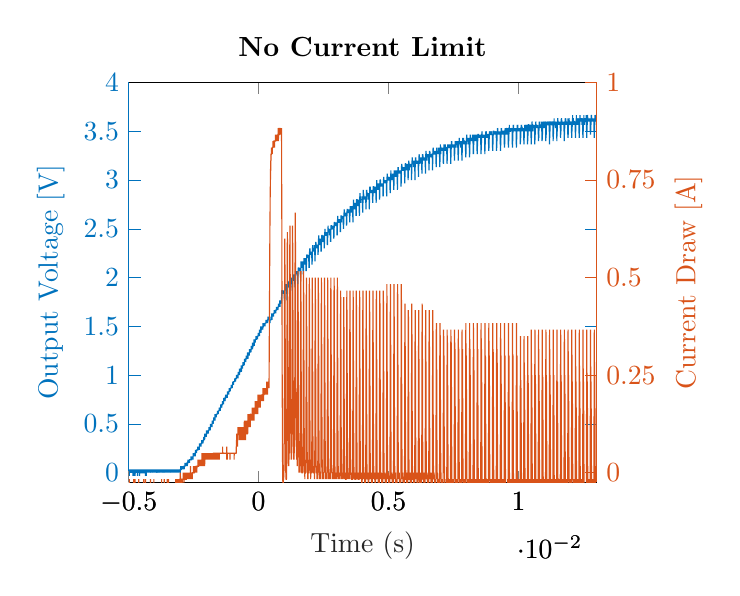
\begin{tikzpicture}

\begin{axis}[%  
width=0.49\textwidth,
height=2in,
at={(0.758in,0.481in)},
scale only axis,
xmin=-0.005,
xmax=0.013,
xlabel style={font=\color{white!15!black}},
xlabel={Time (s)},
separate axis lines,
every outer y axis line/.append style={mycolor1},
every y tick label/.append style={font=\color{mycolor1}},
every y tick/.append style={mycolor1},
ymin=-0.1,
ymax=4,
ytick={  0, 0.5,   1, 1.5,   2, 2.5,   3, 3.5,   4},
ylabel style={font=\color{mycolor1}},
ylabel={Output Voltage [V]},
axis background/.style={fill=white},
title style={font=\bfseries},
title={No Current Limit}
]
\addplot [color=mycolor1, forget plot]
  table[row sep=crcr]{%
-0.00500009950000013	0\\
-0.00499909949999999	0.0333332999999998\\
-0.00499709950000016	0\\
-0.00499689950000004	0.0333332999999998\\
-0.00499509949999988	0\\
-0.0049948995000002	0.0333332999999998\\
-0.00498969949999983	0\\
-0.00498929950000004	0.0333332999999998\\
-0.00498809949999979	0\\
-0.00498789950000011	0.0333332999999998\\
-0.00498509949999981	0\\
-0.00498469950000002	0.0333332999999998\\
-0.00498149949999993	-0.0333332999999998\\
-0.00498129949999981	0.0333332999999998\\
-0.00497609949999989	0\\
-0.00497509950000019	0.0333332999999998\\
-0.00497409950000005	-0.0333332999999998\\
-0.00497309949999991	0.0333332999999998\\
-0.00496869950000001	0\\
-0.00496849949999989	0.0333332999999998\\
-0.00496749950000019	0\\
-0.00496729950000008	0.0333332999999998\\
-0.00496629949999994	0\\
-0.00496609949999982	0.0333332999999998\\
-0.0049642995000001	0\\
-0.00496409949999999	0.0333332999999998\\
-0.00496249949999994	0\\
-0.00496229949999982	0.0333332999999998\\
-0.00496189950000003	0\\
-0.0049614994999998	0.0333332999999998\\
-0.00496109950000001	0\\
-0.00496089949999989	0.0333332999999998\\
-0.0049598995000002	0\\
-0.00495969950000008	0.0333332999999998\\
-0.00495689949999978	0\\
-0.00495669950000011	0.0333332999999998\\
-0.00495549949999985	0\\
-0.00495529950000018	0.0333332999999998\\
-0.00495429950000004	0\\
-0.00495409949999992	0.0333332999999998\\
-0.0049538994999998	0\\
-0.00495369950000013	0.0333332999999998\\
-0.00495309949999978	0\\
-0.00495289950000011	0.0333332999999998\\
-0.00495189949999997	0\\
-0.00495169949999985	0.0333332999999998\\
-0.00495069950000016	0\\
-0.00495049950000004	0.0333332999999998\\
-0.00494969950000002	0\\
-0.0049494994999999	0.0333332999999998\\
-0.00494929949999978	0\\
-0.00494909950000011	0.0333332999999998\\
-0.00494829950000009	0\\
-0.00494809949999997	0.0333332999999998\\
-0.00494709949999983	0\\
-0.00494669950000004	0.0333332999999998\\
-0.00494609950000013	0\\
-0.00494589950000002	0.0333332999999998\\
-0.00494509949999999	0\\
-0.00494489949999988	0.0333332999999998\\
-0.00494349949999995	0\\
-0.00494329949999983	0.0333332999999998\\
-0.00493929950000016	0\\
-0.00493909950000004	0.0333332999999998\\
-0.00493509949999993	0\\
-0.00493489949999981	0.0333332999999998\\
-0.00493329950000021	0\\
-0.00493309950000009	0.0333332999999998\\
-0.00493249950000019	0\\
-0.00493229950000007	0.0333332999999998\\
-0.0049298995	0\\
-0.00492969949999988	0.0333332999999998\\
-0.00492929950000009	0\\
-0.00492909949999998	0.0333332999999998\\
-0.00492809949999984	0\\
-0.00492789950000017	0.0333332999999998\\
-0.00492769950000005	0\\
-0.00492749949999993	0.0333332999999998\\
-0.00492729949999982	0\\
-0.00492709950000014	0.0333332999999998\\
-0.00492429949999984	0\\
-0.00492409950000017	0.0333332999999998\\
-0.00492129949999986	0\\
-0.00492109950000019	0.0333332999999998\\
-0.00491969949999982	0\\
-0.00491929950000003	0.0333332999999998\\
-0.00491909949999991	0\\
-0.0049188994999998	0.0333332999999998\\
-0.00491869950000012	0\\
-0.00491849950000001	0.0333332999999998\\
-0.00491829949999989	0\\
-0.00491809950000022	0.0333332999999998\\
-0.00491649950000017	0\\
-0.00491629950000005	0.0333332999999998\\
-0.00491389949999999	0\\
-0.00491369949999987	0.0333332999999998\\
-0.00491329950000008	0\\
-0.00491309949999996	0.0333332999999998\\
-0.00491169950000003	0\\
-0.00491149949999992	0.0333332999999998\\
-0.00491069949999989	0\\
-0.00491049950000022	0.0333332999999998\\
-0.00490929949999996	0\\
-0.00490909949999985	0.0333332999999998\\
-0.00490789950000003	0\\
-0.00490769949999992	0.0333332999999998\\
-0.00490709950000001	0\\
-0.00490689949999989	0.0333332999999998\\
-0.00490629949999999	0\\
-0.00490609949999987	0.0333332999999998\\
-0.00490449949999983	0\\
-0.00490429950000015	0.0333332999999998\\
-0.00490409950000004	0\\
-0.0049036994999998	0.0333332999999998\\
-0.00490289949999978	0\\
-0.00490269950000011	0.0333332999999998\\
-0.00490249949999999	0\\
-0.00490229949999987	0.0333332999999998\\
-0.00490069949999983	0\\
-0.00490049950000015	0.0333332999999998\\
-0.00489789949999997	0\\
-0.00489749950000018	0.0333332999999998\\
-0.00489569950000002	0\\
-0.00489529949999978	0.0333332999999998\\
-0.00489289950000016	0\\
-0.00489269950000004	0.0333332999999998\\
-0.0048916994999999	0\\
-0.00489149949999979	0.0333332999999998\\
-0.00489029949999997	0\\
-0.00489009949999986	0.0333332999999998\\
-0.00488769949999979	0\\
-0.00488749950000011	0.0333332999999998\\
-0.0048872995	0\\
-0.00488709949999988	0.0333332999999998\\
-0.00488569949999995	0\\
-0.00488549949999983	0.0333332999999998\\
-0.00488529950000016	0\\
-0.00488509950000005	0.0333332999999998\\
-0.00488489949999993	0\\
-0.00488469949999981	0.0333332999999998\\
-0.00488369950000012	0\\
-0.0048834995	0.0333332999999998\\
-0.00488029949999991	0\\
-0.0048796995	0.0333332999999998\\
-0.00487909950000009	0\\
-0.00487889949999998	0.0333332999999998\\
-0.00487849950000019	0\\
-0.00487809949999995	0.0333332999999998\\
-0.00487449950000007	0\\
-0.00487429949999996	0.0333332999999998\\
-0.00487389950000017	0\\
-0.00487329949999982	0.0333332999999998\\
-0.00487129949999998	0\\
-0.00487109949999986	0.0333332999999998\\
-0.00486949949999982	0\\
-0.00486929950000015	0.0333332999999998\\
-0.00486409950000022	0\\
-0.00486049949999989	0.0333332999999998\\
-0.00485889949999985	0\\
-0.00485869950000017	0.0333332999999998\\
-0.00485809949999982	0\\
-0.00485789950000015	0.0333332999999998\\
-0.00485629950000011	0\\
-0.00485609949999999	0.0333332999999998\\
-0.00485389950000004	0\\
-0.00485369949999992	0.0333332999999998\\
-0.00485269949999978	0\\
-0.00485249950000011	0.0333332999999998\\
-0.00485149949999997	0\\
-0.00485129949999985	0.0333332999999998\\
-0.00485009950000004	0\\
-0.00484989949999992	0.0333332999999998\\
-0.00484469949999999	0\\
-0.00484289949999983	0.0333332999999998\\
-0.00484189950000014	0\\
-0.00484169950000002	0.0333332999999998\\
-0.00484009949999997	0\\
-0.00483989949999986	0.0333332999999998\\
-0.00483929949999995	0\\
-0.00483909949999983	0.0333332999999998\\
-0.00483849949999993	0\\
-0.00483829949999981	0.0333332999999998\\
-0.00483729950000011	-0.0333332999999998\\
-0.00483689949999988	0.0333332999999998\\
-0.00483669950000021	0\\
-0.00483649950000009	0.0333332999999998\\
-0.00483589950000018	0\\
-0.00483569950000007	0.0333332999999998\\
-0.00483529949999983	0\\
-0.00483509950000016	0.0333332999999998\\
-0.00483349950000012	0\\
-0.0048332995	0.0333332999999998\\
-0.00483149949999984	0\\
-0.00483129950000016	0.0333332999999998\\
-0.00483069949999981	0\\
-0.00483049950000014	0.0333332999999998\\
-0.00482529950000021	0\\
-0.00482229949999979	0.0333332999999998\\
-0.00482209950000012	0\\
-0.0048218995	0.0333332999999998\\
-0.00482149950000021	0\\
-0.00482109949999998	0.0333332999999998\\
-0.00481589950000005	0\\
-0.00481449950000012	0.0333332999999998\\
-0.0048092995000002	0\\
-0.00480789949999982	0.0333332999999998\\
-0.00480749950000003	0\\
-0.00480729949999992	0.0333332999999998\\
-0.00480509949999997	0\\
-0.00480489949999985	0.0333332999999998\\
-0.00479969949999992	0\\
-0.00479929950000013	0.0333332999999998\\
-0.00479909950000001	0\\
-0.0047988994999999	0.0333332999999998\\
-0.00479769950000009	-0.0333332999999998\\
-0.00479549950000013	0.0333332999999998\\
-0.00479529950000002	0\\
-0.0047950994999999	0.0333332999999998\\
-0.0047940995000002	0\\
-0.00479389950000009	0.0333332999999998\\
-0.00479349949999985	0\\
-0.00479309950000006	0.0333332999999998\\
-0.00479269949999983	0\\
-0.00479249950000016	0.0333332999999998\\
-0.00479169950000014	0\\
-0.00479149950000002	0.0333332999999998\\
-0.00478889949999983	0\\
-0.00478869950000016	0.0333332999999998\\
-0.00478629950000009	0\\
-0.00478609949999997	0.0333332999999998\\
-0.00478229949999998	0\\
-0.00478209949999986	0.0333332999999998\\
-0.00477709950000005	0\\
-0.00477689949999993	0.0333332999999998\\
-0.00477569950000012	0\\
-0.0047754995	0.0333332999999998\\
-0.00477449949999986	0\\
-0.00477429950000019	0.0333332999999998\\
-0.0047710995000001	0\\
-0.00477089949999998	0.0333332999999998\\
-0.00477009949999996	0\\
-0.00476989949999984	0.0333332999999998\\
-0.00476949950000005	-0.0333332999999998\\
-0.00476909949999982	0.0333332999999998\\
-0.00476389949999989	0\\
-0.0047568994999998	0\\
-0.00475669950000013	0.0333332999999998\\
-0.00475389949999983	0\\
-0.00475369950000015	0.0333332999999998\\
-0.00475209950000011	-0.0333332999999998\\
-0.00474809949999999	0.0333332999999998\\
-0.00474669950000006	0\\
-0.00474649949999995	0.0333332999999998\\
-0.00474629949999983	0\\
-0.00474609950000016	0.0333332999999998\\
-0.00474549949999981	0\\
-0.00474529950000013	0.0333332999999998\\
-0.00474509950000002	0\\
-0.0047448994999999	0.0333332999999998\\
-0.00474189949999992	0\\
-0.00474169949999981	0.0333332999999998\\
-0.00474069950000011	0\\
-0.00474009950000021	0.0333332999999998\\
-0.00473829950000004	0\\
-0.00473809949999993	0.0333332999999998\\
-0.00473609950000009	0\\
-0.00473589949999997	0.0333332999999998\\
-0.00473449950000004	0\\
-0.00473409949999981	0.0333332999999998\\
-0.00473369950000002	0\\
-0.0047334994999999	0.0333332999999998\\
-0.00473209949999998	0\\
-0.00473169950000019	0.0333332999999998\\
-0.00472769950000007	0\\
-0.00472749949999995	0.0333332999999998\\
-0.00472729949999984	0\\
-0.00472709950000016	0.0333332999999998\\
-0.00472489950000021	0\\
-0.00472449949999998	0.0333332999999998\\
-0.00472249950000014	0\\
-0.00472229950000003	0.0333332999999998\\
-0.00471809949999979	0\\
-0.00471769950000001	0.0333332999999998\\
-0.00471749949999989	0\\
-0.00471729950000022	0.0333332999999998\\
-0.00471649950000019	0\\
-0.00471629950000008	0.0333332999999998\\
-0.00471549950000005	0\\
-0.00471529949999994	0.0333332999999998\\
-0.00471089950000003	0\\
-0.00471069949999992	0.0333332999999998\\
-0.00470989949999989	0\\
-0.00470969950000022	0.0333332999999998\\
-0.00470929949999999	0\\
-0.00470909949999987	0.0333332999999998\\
-0.0047088995000002	0\\
-0.00470869950000008	0.0333332999999998\\
-0.00470749949999982	0\\
-0.00470729950000015	0.0333332999999998\\
-0.00470529949999987	0\\
-0.0047050995000002	0.0333332999999998\\
-0.00470409950000006	0\\
-0.00470389949999994	0.0333332999999998\\
-0.00470269950000013	0\\
-0.00470249950000001	0.0333332999999998\\
-0.00470189950000011	0\\
-0.00470169949999999	0.0333332999999998\\
-0.00470089949999997	0\\
-0.00470009949999994	0.0333332999999998\\
-0.0046974995000002	0\\
-0.00469709949999997	0.0333332999999998\\
-0.00469689949999985	0\\
-0.00469669950000018	0.0333332999999998\\
-0.00469629949999995	0\\
-0.00469609949999983	0.0333332999999998\\
-0.00469529949999981	0\\
-0.00469509950000013	0.0333332999999998\\
-0.00468989950000021	0\\
-0.00468829950000016	0.0333332999999998\\
-0.00468609950000021	0\\
-0.00468589950000009	0.0333332999999998\\
-0.00468389949999981	0\\
-0.00468369950000014	0.0333332999999998\\
-0.00468029949999993	0\\
-0.00468009949999981	0.0333332999999998\\
-0.00467849950000021	0\\
-0.00467829950000009	0.0333332999999998\\
-0.00467749950000007	0\\
-0.00467729949999995	0.0333332999999998\\
-0.0046744995000001	0\\
-0.00467429949999998	0.0333332999999998\\
-0.0046712995	0\\
-0.00467109949999989	0.0333332999999998\\
-0.00467049949999998	0\\
-0.00467029949999986	0.0333332999999998\\
-0.00466889949999993	0\\
-0.00466869949999982	0.0333332999999998\\
-0.00466849950000015	0\\
-0.00466829950000003	0.0333332999999998\\
-0.00466809949999991	0\\
-0.00466789949999979	0.0333332999999998\\
-0.00466609950000008	0\\
-0.00466589949999996	0.0333332999999998\\
-0.00466429949999991	0\\
-0.0046640994999998	0.0333332999999998\\
-0.00465969949999989	-0.0333332999999998\\
-0.00465629950000013	0.0333332999999998\\
-0.00465469950000008	0\\
-0.00465449949999996	0.0333332999999998\\
-0.0046520994999999	0\\
-0.00465189949999978	0.0333332999999998\\
-0.00464669949999985	0\\
-0.00464649950000018	0.0333332999999998\\
-0.00464569950000016	0\\
-0.00464549950000004	0.0333332999999998\\
-0.00464029950000011	0\\
-0.00463709950000002	0.0333332999999998\\
-0.00463189950000009	0\\
-0.00463129950000019	0.0333332999999998\\
-0.00462969950000014	0\\
-0.00462949950000002	0.0333332999999998\\
-0.00462929949999991	0\\
-0.00462909949999979	0.0333332999999998\\
-0.00462549949999991	0\\
-0.00462529949999979	0.0333332999999998\\
-0.00462449950000021	0\\
-0.0046242995000001	0.0333332999999998\\
-0.00462309949999984	0\\
-0.00462289950000017	0.0333332999999998\\
-0.00461869949999993	0\\
-0.00461849949999982	0.0333332999999998\\
-0.0046166995000001	0\\
-0.00461649949999998	0.0333332999999998\\
-0.00461129950000005	0\\
-0.00460789949999985	0.0333332999999998\\
-0.00460769950000017	0\\
-0.00460749950000006	0.0333332999999998\\
-0.00460669950000003	0\\
-0.00460649949999992	0.0333332999999998\\
-0.00460569949999989	0\\
-0.00460549950000022	0.0333332999999998\\
-0.00460069950000008	0\\
-0.00460049949999997	0.0333332999999998\\
-0.00460029949999985	0\\
-0.00460009950000018	0.0333332999999998\\
-0.00459949949999983	0\\
-0.00459929950000015	0.0333332999999998\\
-0.00459409949999978	0\\
-0.00459349949999988	0.0333332999999998\\
-0.0045904994999999	0\\
-0.00459029949999978	0.0333332999999998\\
-0.00458909949999997	0\\
-0.00458889949999985	0.0333332999999998\\
-0.00458869950000018	0\\
-0.00458849950000007	0.0333332999999998\\
-0.00458689950000002	-0.0333332999999998\\
-0.00458169950000009	0\\
-0.00457829949999988	0.0333332999999998\\
-0.00457649950000016	0\\
-0.00457629950000005	0.0333332999999998\\
-0.00457349950000019	0\\
-0.00457329950000007	0.0333332999999998\\
-0.00457309949999996	0\\
-0.00457289949999984	0.0333332999999998\\
-0.00457229949999993	0\\
-0.00457209949999982	0.0333332999999998\\
-0.0045708995	0\\
-0.0045702995000001	0.0333332999999998\\
-0.00456749949999979	0\\
-0.00456729950000012	0.0333332999999998\\
-0.00456429950000015	0\\
-0.00456409950000003	0.0333332999999998\\
-0.0045588995000001	0\\
-0.0045550995000001	0.0333332999999998\\
-0.0045506995000002	0\\
-0.00455049950000008	0.0333332999999998\\
-0.00454829950000013	0\\
-0.00454809950000001	0.0333332999999998\\
-0.00454289950000009	0\\
-0.00453569949999988	0\\
-0.00453549950000021	0.0333332999999998\\
-0.00453469950000018	0\\
-0.00453449950000007	0.0333332999999998\\
-0.00453429949999995	0\\
-0.00453409949999983	0.0333332999999998\\
-0.00453249949999979	0\\
-0.00453229950000011	0.0333332999999998\\
-0.0045320995	0\\
-0.00453189949999988	0.0333332999999998\\
-0.00452729949999986	0\\
-0.00452709950000019	0.0333332999999998\\
-0.00452289949999995	0\\
-0.00452249950000017	0.0333332999999998\\
-0.0045206995	0\\
-0.00452049949999989	0.0333332999999998\\
-0.00451549950000008	0\\
-0.00451529949999996	0.0333332999999998\\
-0.00451329950000012	0\\
-0.00451309950000001	0.0333332999999998\\
-0.00451009950000003	0\\
-0.00450989949999991	0.0333332999999998\\
-0.00450469949999999	0\\
-0.00449789950000001	0\\
-0.0044976994999999	0.0333332999999998\\
-0.00449649950000008	0\\
-0.00449629949999997	0.0333332999999998\\
-0.00449569950000006	0\\
-0.00449549949999994	0.0333332999999998\\
-0.00449029950000002	0\\
-0.00448509950000009	0\\
-0.00448489949999997	0.0333332999999998\\
-0.00448429950000007	0\\
-0.00448409949999995	0.0333332999999998\\
-0.00448329949999993	0\\
-0.00448309949999981	0.0333332999999998\\
-0.00447889950000002	0\\
-0.00447869949999991	0.0333332999999998\\
-0.00447689950000019	0\\
-0.00447669950000007	0.0333332999999998\\
-0.00447469949999979	0\\
-0.00447449950000012	0.0333332999999998\\
-0.00447349949999998	0\\
-0.00447329949999986	0.0333332999999998\\
-0.00447229950000017	0\\
-0.00447209950000005	0.0333332999999998\\
-0.00447149950000014	0\\
-0.00447109949999991	0.0333332999999998\\
-0.00447069950000012	0\\
-0.00447029949999989	0.0333332999999998\\
-0.00446769950000014	0\\
-0.00446749950000003	0.0333332999999998\\
-0.00446649949999989	0\\
-0.00446629950000021	0.0333332999999998\\
-0.00446429949999994	0\\
-0.00446409949999982	0.0333332999999998\\
-0.00446349949999991	0\\
-0.0044632994999998	0.0333332999999998\\
-0.00446009950000015	0\\
-0.00445989950000003	0.0333332999999998\\
-0.0044594994999998	0\\
-0.00445929950000012	0.0333332999999998\\
-0.00445869950000022	0\\
-0.0044584995000001	0.0333332999999998\\
-0.00445709950000017	0\\
-0.00445689950000006	0.0333332999999998\\
-0.00445629950000015	0\\
-0.0044556994999998	0.0333332999999998\\
-0.00445049949999987	0\\
-0.00444489950000015	0\\
-0.00444469950000004	0.0333332999999998\\
-0.00444349949999978	0\\
-0.00444329950000011	0.0333332999999998\\
-0.00444249950000009	0\\
-0.00444229949999997	0.0333332999999998\\
-0.00444169950000006	0\\
-0.00444149949999995	0.0333332999999998\\
-0.00444129949999983	0\\
-0.00444109950000016	0.0333332999999998\\
-0.00444049949999981	0\\
-0.00444029950000013	0.0333332999999998\\
-0.00443829949999985	0\\
-0.00443789950000006	0.0333332999999998\\
-0.00443629950000002	0\\
-0.00443589949999978	0.0333332999999998\\
-0.00443449949999986	0\\
-0.00443429950000018	0.0333332999999998\\
-0.00443409950000007	0\\
-0.00443389949999995	0.0333332999999998\\
-0.00443369949999983	0\\
-0.00443349950000016	0.0333332999999998\\
-0.00443209949999979	0\\
-0.00443189950000011	0.0333332999999998\\
-0.00443129950000021	0\\
-0.00443109950000009	0.0333332999999998\\
-0.00442589950000016	0\\
-0.00442349950000009	0.0333332999999998\\
-0.00442289950000019	0\\
-0.00442229949999984	0.0333332999999998\\
-0.0044196995000001	0\\
-0.00441949949999998	0.0333332999999998\\
-0.00441769949999982	0\\
-0.00441729950000003	0.0333332999999998\\
-0.00441709949999991	0\\
-0.00441689949999979	0.0333332999999998\\
-0.00441429950000005	0\\
-0.00441409949999994	0.0333332999999998\\
-0.00441289950000012	0\\
-0.00441269950000001	0.0333332999999998\\
-0.00441169949999987	0\\
-0.00441149950000019	0.0333332999999998\\
-0.00441089949999984	0\\
-0.00441069950000017	0.0333332999999998\\
-0.00440969950000003	0\\
-0.00440949949999991	0.0333332999999998\\
-0.00440669950000006	0\\
-0.00440649949999994	0.0333332999999998\\
-0.00440129950000001	0\\
-0.00439329949999978	0\\
-0.00439309950000011	0.0333332999999998\\
-0.00438909949999999	0\\
-0.00438889949999988	0.0333332999999998\\
-0.00438369949999995	0\\
-0.00438049949999986	0.0333332999999998\\
-0.00437849950000002	0\\
-0.0043782994999999	0.0333332999999998\\
-0.00437809949999979	0\\
-0.00437789950000012	0.0333332999999998\\
-0.00437529949999993	0\\
-0.00437509949999981	0.0333332999999998\\
-0.00437409950000012	0\\
-0.0043738995	0.0333332999999998\\
-0.00437249950000007	0\\
-0.00437229949999995	0.0333332999999998\\
-0.00437149949999993	0\\
-0.00437129949999981	0.0333332999999998\\
-0.00436969950000021	0\\
-0.0043694995000001	0.0333332999999998\\
-0.00436489950000007	0\\
-0.00436469949999996	0.0333332999999998\\
-0.00436209950000022	0\\
-0.00436169949999998	0.0333332999999998\\
-0.00436109950000008	0\\
-0.00436089949999996	0.0333332999999998\\
-0.00436009949999994	-0.0333332999999998\\
-0.00435489950000001	0\\
-0.00435209950000015	0.0333332999999998\\
-0.00435129950000013	0\\
-0.00435089949999989	0.0333332999999998\\
-0.00434569949999997	0\\
-0.00434169949999985	0.0333332999999998\\
-0.00433709949999983	0\\
-0.00433689950000016	0.0333332999999998\\
-0.00433589950000002	0\\
-0.0043356994999999	0.0333332999999998\\
-0.0043312995	0\\
-0.00433109949999988	0.0333332999999998\\
-0.00432889949999993	0\\
-0.00432869949999981	0.0333332999999998\\
-0.00432829950000002	0\\
-0.0043280994999999	0.0333332999999998\\
-0.00432409949999979	-0.0333332999999998\\
-0.00432349949999988	0.0333332999999998\\
-0.00432289949999998	0\\
-0.00432269949999986	0.0333332999999998\\
-0.00432209949999995	0\\
-0.00432189949999984	0.0333332999999998\\
-0.00432009950000012	0\\
-0.0043198995	0.0333332999999998\\
-0.00431949950000021	0\\
-0.0043192995000001	0.0333332999999998\\
-0.00431909949999998	0\\
-0.00431889949999986	0.0333332999999998\\
-0.00431749949999993	0\\
-0.00431729949999982	0.0333332999999998\\
-0.00431309950000003	0\\
-0.00431289949999991	0.0333332999999998\\
-0.00430949950000015	0\\
-0.00430929950000003	0.0333332999999998\\
-0.00430669949999984	0\\
-0.00430649950000017	0.0333332999999998\\
-0.00430589949999982	0\\
-0.00430569950000015	0.0333332999999998\\
-0.0043040995000001	0\\
-0.00430369949999987	0.0333332999999998\\
-0.00430169950000003	0\\
-0.00430149949999992	0.0333332999999998\\
-0.00429989949999987	0\\
-0.0042996995000002	0.0333332999999998\\
-0.00429769949999992	0\\
-0.0042974994999998	0.0333332999999998\\
-0.00429489950000006	0\\
-0.00429469949999994	0.0333332999999998\\
-0.00428949950000002	0\\
-0.00428769949999985	0.0333332999999998\\
-0.00428649950000004	0\\
-0.00428629949999992	0.0333332999999998\\
-0.00428429950000009	0\\
-0.00428409949999997	0.0333332999999998\\
-0.00428049950000009	0\\
-0.00428029949999997	0.0333332999999998\\
-0.00427709949999988	0\\
-0.00427689950000021	0.0333332999999998\\
-0.00427569949999995	0\\
-0.00427549949999984	0.0333332999999998\\
-0.00427489949999993	0\\
-0.00427469949999981	0.0333332999999998\\
-0.0042734995	0\\
-0.00427329949999988	0.0333332999999998\\
-0.00427069950000014	0\\
-0.00427049950000002	0.0333332999999998\\
-0.00426929950000021	0\\
-0.0042690995000001	0.0333332999999998\\
-0.0042658995	0\\
-0.00426569949999989	0.0333332999999998\\
-0.00426449950000007	0\\
-0.00426429949999996	0.0333332999999998\\
-0.00426109949999987	0\\
-0.00426069950000008	0.0333332999999998\\
-0.00425829950000001	0\\
-0.00425809949999989	0.0333332999999998\\
-0.00425709950000019	0\\
-0.00425689950000008	0.0333332999999998\\
-0.0042538995000001	0\\
-0.00425369949999999	0.0333332999999998\\
-0.00425209949999994	0\\
-0.00425189949999982	0.0333332999999998\\
-0.00425049949999989	0\\
-0.00425029950000022	0.0333332999999998\\
-0.0042500995000001	0\\
-0.00424989949999999	0.0333332999999998\\
-0.00424689950000001	0\\
-0.0042466994999999	0.0333332999999998\\
-0.0042456995000002	0\\
-0.00424529949999997	0.0333332999999998\\
-0.00424509949999985	0\\
-0.00424489950000018	0.0333332999999998\\
-0.00424369949999992	0\\
-0.0042434994999998	0.0333332999999998\\
-0.0042428994999999	0\\
-0.00424269949999978	0.0333332999999998\\
-0.00424229949999999	0\\
-0.0042418995000002	0.0333332999999998\\
-0.00424149949999997	0\\
-0.00424129949999985	0.0333332999999998\\
-0.00424069949999994	0\\
-0.00424029950000016	0.0333332999999998\\
-0.00424009950000004	0\\
-0.00423989949999992	0.0333332999999998\\
-0.00423869950000011	0\\
-0.00423849949999999	0.0333332999999998\\
-0.00423829949999988	0\\
-0.0042380995000002	0.0333332999999998\\
-0.00423729950000018	0\\
-0.00423709950000006	0.0333332999999998\\
-0.00423629950000004	0\\
-0.00423609949999992	0.0333332999999998\\
-0.0042314994999999	0\\
-0.00423129949999979	0.0333332999999998\\
-0.00422969950000018	0\\
-0.00422949950000007	0.0333332999999998\\
-0.00422929949999995	0\\
-0.00422909949999983	0.0333332999999998\\
-0.00422809950000014	0\\
-0.0042276994999999	0.0333332999999998\\
-0.00422529949999984	0\\
-0.00422509950000016	0.0333332999999998\\
-0.00422489950000005	0\\
-0.00422469949999993	0.0333332999999998\\
-0.00422209950000019	0\\
-0.00422189950000007	0.0333332999999998\\
-0.00422089949999993	0\\
-0.00422069949999981	0.0333332999999998\\
-0.00421849949999986	0\\
-0.00421829950000019	0.0333332999999998\\
-0.00421529950000021	0\\
-0.0042150995000001	0.0333332999999998\\
-0.00421329949999993	0\\
-0.00421309949999982	0.0333332999999998\\
-0.00421109949999998	0\\
-0.00421089949999987	0.0333332999999998\\
-0.00420809950000001	0\\
-0.00420789949999989	0.0333332999999998\\
-0.00420609950000017	0\\
-0.00420589950000005	0.0333332999999998\\
-0.00420489949999991	0\\
-0.0042046994999998	0.0333332999999998\\
-0.00420449950000013	0\\
-0.00420429950000001	0.0333332999999998\\
-0.00420209950000006	0\\
-0.00420189949999994	0.0333332999999998\\
-0.00420149950000015	0\\
-0.00420109949999992	0.0333332999999998\\
-0.00420049950000001	0\\
-0.00420029949999989	0.0333332999999998\\
-0.00419949949999987	0\\
-0.0041992995000002	0.0333332999999998\\
-0.00419909950000008	0\\
-0.00419889949999996	0.0333332999999998\\
-0.00419809949999994	0\\
-0.00419769950000015	0.0333332999999998\\
-0.00419689950000013	0\\
-0.00419669950000001	0.0333332999999998\\
-0.0041964994999999	0\\
-0.00419629950000022	0.0333332999999998\\
-0.00419569949999987	0\\
-0.0041954995000002	0.0333332999999998\\
-0.00419509949999997	0\\
-0.00419489949999985	0.0333332999999998\\
-0.00419389950000015	0\\
-0.00419369950000004	0.0333332999999998\\
-0.00419189949999987	0\\
-0.0041916995000002	0.0333332999999998\\
-0.00419129949999997	0\\
-0.00419109949999985	0.0333332999999998\\
-0.00419089950000018	0\\
-0.00419049949999994	0.0333332999999998\\
-0.00418969949999992	0\\
-0.0041894994999998	0.0333332999999998\\
-0.00418829949999999	0\\
-0.0041878995000002	0.0333332999999998\\
-0.00418769950000009	0\\
-0.00418749949999997	0.0333332999999998\\
-0.00418469950000011	0\\
-0.00418449949999999	0.0333332999999998\\
-0.00418389950000009	0\\
-0.00418349949999985	0.0333332999999998\\
-0.00418309950000006	0\\
-0.00418289949999995	0.0333332999999998\\
-0.00418189949999981	0\\
-0.00418149950000002	0.0333332999999998\\
-0.00417909949999995	0\\
-0.00417869950000016	0.0333332999999998\\
-0.00417789950000014	0\\
-0.00417769950000002	0.0333332999999998\\
-0.00417709950000011	0\\
-0.0041768995	0.0333332999999998\\
-0.00417509949999983	0\\
-0.00417489950000016	0.0333332999999998\\
-0.00417229949999998	0\\
-0.00417209949999986	0.0333332999999998\\
-0.00417029950000014	0\\
-0.00417009950000002	0.0333332999999998\\
-0.00416829949999986	0\\
-0.00416809950000019	0.0333332999999998\\
-0.00416709950000005	0\\
-0.00416689949999993	0.0333332999999998\\
-0.00416569950000012	0\\
-0.00416529949999989	0.0333332999999998\\
-0.00416509950000021	0\\
-0.0041648995000001	0.0333332999999998\\
-0.00416269950000014	0\\
-0.00416249950000003	0.0333332999999998\\
-0.00416009949999996	0\\
-0.00415989949999984	0.0333332999999998\\
-0.00415969950000017	0\\
-0.00415949950000005	0.0333332999999998\\
-0.00415789950000001	0\\
-0.00415769949999989	0.0333332999999998\\
-0.00415709949999998	0\\
-0.00415689949999987	0.0333332999999998\\
-0.00415669950000019	0\\
-0.00415649950000008	0.0333332999999998\\
-0.00415609949999984	0\\
-0.00415589950000017	0.0333332999999998\\
-0.00415569950000005	0\\
-0.00415549949999994	0.0333332999999998\\
-0.00415029950000001	0\\
-0.00414929949999987	0.0333332999999998\\
-0.0041490995000002	0\\
-0.00414829950000017	0.0333332999999998\\
-0.00414649950000001	0\\
-0.00414629949999989	0.0333332999999998\\
-0.00414609950000022	0\\
-0.00414589950000011	0.0333332999999998\\
-0.00414569949999999	0\\
-0.00414549949999987	0.0333332999999998\\
-0.0041452995000002	0\\
-0.00414509950000008	0.0333332999999998\\
-0.00414289950000013	0\\
-0.00414269950000001	0.0333332999999998\\
-0.0041414995000002	0\\
-0.00414129950000008	0.0333332999999998\\
-0.00414009949999983	0\\
-0.00413989950000015	0.0333332999999998\\
-0.00413889950000002	0\\
-0.00413849949999978	0.0333332999999998\\
-0.00413809949999999	0\\
-0.00413789949999988	0.0333332999999998\\
-0.00413749950000009	0\\
-0.00413729949999997	0.0333332999999998\\
-0.0041348994999999	0\\
-0.00413469949999978	0.0333332999999998\\
-0.0041338995000002	0\\
-0.00413369950000009	0.0333332999999998\\
-0.00413329949999985	0\\
-0.00413309950000018	0.0333332999999998\\
-0.00413229950000016	0\\
-0.00413209950000004	0.0333332999999998\\
-0.00413069950000011	0\\
-0.0041304995	0.0333332999999998\\
-0.00413009950000021	0\\
-0.00412989950000009	0.0333332999999998\\
-0.00412909950000007	0\\
-0.00412889949999995	0.0333332999999998\\
-0.00412529950000007	0\\
-0.00412489949999983	0.0333332999999998\\
-0.00412209949999998	0\\
-0.00412189949999986	0.0333332999999998\\
-0.00411969949999991	0\\
-0.00411949949999979	0.0333332999999998\\
-0.00411729949999984	0\\
-0.00411689950000005	0.0333332999999998\\
-0.00411649949999982	0\\
-0.00411629950000014	0.0333332999999998\\
-0.00411329950000017	0\\
-0.00411309950000005	0.0333332999999998\\
-0.00411029950000019	0\\
-0.00411009950000008	0.0333332999999998\\
-0.00410949950000017	0\\
-0.00410909949999994	0.0333332999999998\\
-0.00410889949999982	0\\
-0.00410869950000015	0.0333332999999998\\
-0.00410609949999996	0\\
-0.00410569950000017	0.0333332999999998\\
-0.00410229949999996	0\\
-0.00410209949999985	0.0333332999999998\\
-0.00410109950000015	0\\
-0.00410089950000003	0.0333332999999998\\
-0.00409989949999989	0\\
-0.00409969950000022	0.0333332999999998\\
-0.00409909949999987	0\\
-0.0040988995000002	0.0333332999999998\\
-0.00409729950000015	0\\
-0.00409709950000003	0.0333332999999998\\
-0.00409489950000008	0\\
-0.00409469949999997	0.0333332999999998\\
-0.00409349950000015	0\\
-0.00409309949999992	0.0333332999999998\\
-0.0040928994999998	0\\
-0.00409269950000013	0.0333332999999998\\
-0.00409209949999978	0\\
-0.00409189950000011	0.0333332999999998\\
-0.00409109950000008	0\\
-0.00409089949999997	0.0333332999999998\\
-0.00409029950000006	0\\
-0.00409009949999994	0.0333332999999998\\
-0.00408949950000004	0\\
-0.00408929949999992	0.0333332999999998\\
-0.00408729950000009	0\\
-0.00408709949999997	0.0333332999999998\\
-0.00408689949999985	0\\
-0.00408669950000018	0.0333332999999998\\
-0.00408629949999995	0\\
-0.00408609949999983	0.0333332999999998\\
-0.00408529949999981	0\\
-0.00408489950000002	0.0333332999999998\\
-0.00408329949999997	0\\
-0.00408309949999985	0.0333332999999998\\
-0.00408149949999981	0\\
-0.0040808994999999	0.0333332999999998\\
-0.00408009949999988	0\\
-0.00407989950000021	0.0333332999999998\\
-0.00407949949999997	0\\
-0.00407929949999986	0.0333332999999998\\
-0.00407889950000007	0\\
-0.00407869949999995	0.0333332999999998\\
-0.00407849949999983	0\\
-0.00407829950000016	0.0333332999999998\\
-0.00407729950000002	0\\
-0.0040770994999999	0.0333332999999998\\
-0.0040764995	0\\
-0.00407629949999988	0.0333332999999998\\
-0.00407609950000021	0\\
-0.00407589950000009	0.0333332999999998\\
-0.00407369950000014	0\\
-0.00407349950000002	0.0333332999999998\\
-0.00407189949999998	0\\
-0.00407169949999986	0.0333332999999998\\
-0.00407129950000007	0\\
-0.00407109949999995	0.0333332999999998\\
-0.00407069950000016	0\\
-0.00407049950000005	0.0333332999999998\\
-0.00406669950000005	0\\
-0.00406649949999993	0.0333332999999998\\
-0.00406609950000014	0\\
-0.00406589950000003	0.0333332999999998\\
-0.00406549949999979	0\\
-0.00406529950000012	0.0333332999999998\\
-0.0040650995	0\\
-0.00406489949999989	0.0333332999999998\\
-0.00406429949999998	0\\
-0.00406389950000019	0.0333332999999998\\
-0.00406269949999993	0\\
-0.00406249949999982	0.0333332999999998\\
-0.00406109949999989	0\\
-0.00406089950000021	0.0333332999999998\\
-0.00406049949999998	0\\
-0.00406009950000019	0.0333332999999998\\
-0.00405489949999982	0\\
-0.00405429949999991	0.0333332999999998\\
-0.00405389950000012	0\\
-0.00405369950000001	0.0333332999999998\\
-0.00405149950000006	0\\
-0.00405109949999982	0.0333332999999998\\
-0.0040502994999998	0\\
-0.00404989950000001	0.0333332999999998\\
-0.0040486995000002	0\\
-0.00404849950000008	0.0333332999999998\\
-0.00404789950000017	0\\
-0.00404769950000006	0.0333332999999998\\
-0.00404629950000013	0\\
-0.00404609950000001	0.0333332999999998\\
-0.00404589949999989	0\\
-0.00404569950000022	0.0333332999999998\\
-0.00404529949999999	0\\
-0.00404509949999987	0.0333332999999998\\
-0.0040448995000002	0\\
-0.00404469950000008	0.0333332999999998\\
-0.00404409950000018	0\\
-0.00404389950000006	0.0333332999999998\\
-0.00404309950000004	0\\
-0.0040426994999998	0.0333332999999998\\
-0.00403809949999978	0\\
-0.00403789950000011	0.0333332999999998\\
-0.00403649950000018	0\\
-0.00403629950000006	0.0333332999999998\\
-0.00403529949999992	0\\
-0.00403509949999981	0.0333332999999998\\
-0.00403469950000002	0\\
-0.0040344994999999	0.0333332999999998\\
-0.00403409950000011	0\\
-0.00403389949999999	0.0333332999999998\\
-0.0040300995	0\\
-0.00402989949999988	0.0333332999999998\\
-0.00402869950000007	0\\
-0.00402849949999995	0.0333332999999998\\
-0.00402829949999983	0\\
-0.00402809950000016	0.0333332999999998\\
-0.00402489950000007	0\\
-0.00402469949999995	0.0333332999999998\\
-0.00402229949999988	0\\
-0.00402209950000021	0.0333332999999998\\
-0.00401949950000002	0\\
-0.00401929949999991	0.0333332999999998\\
-0.00401709949999995	0\\
-0.00401689949999984	0.0333332999999998\\
-0.00401409949999998	0\\
-0.00401389949999986	0.0333332999999998\\
-0.00401369950000019	0\\
-0.00401349950000007	0.0333332999999998\\
-0.00401149949999979	0\\
-0.00401129950000012	0.0333332999999998\\
-0.00400849949999982	0\\
-0.00400829950000015	0.0333332999999998\\
-0.00400589950000008	0\\
-0.00400569949999996	0.0333332999999998\\
-0.00400229950000019	0\\
-0.00400209950000008	0.0333332999999998\\
-0.00399949949999989	0\\
-0.00399929950000022	0.0333332999999998\\
-0.00399709949999982	0\\
-0.00399669950000003	0.0333332999999998\\
-0.00399349949999994	0\\
-0.00399329949999983	0.0333332999999998\\
-0.00399289950000004	0\\
-0.00399269949999992	0.0333332999999998\\
-0.00399109949999987	0\\
-0.0039908995000002	0.0333332999999998\\
-0.00398909950000004	0\\
-0.00398889949999992	0.0333332999999998\\
-0.00398529950000004	0\\
-0.00398449950000002	0.0333332999999998\\
-0.00398409949999978	0\\
-0.00398369949999999	0.0333332999999998\\
-0.0039832995000002	0\\
-0.00398309950000009	0.0333332999999998\\
-0.00398269949999985	0\\
-0.00398249950000018	0.0333332999999998\\
-0.00398169950000016	0\\
-0.00398149950000004	0.0333332999999998\\
-0.00397989949999999	0\\
-0.00397969949999988	0.0333332999999998\\
-0.00397929950000009	0\\
-0.00397909949999997	0.0333332999999998\\
-0.00397869950000018	0\\
-0.00397849950000007	0.0333332999999998\\
-0.00397689950000002	0\\
-0.0039766994999999	0.0333332999999998\\
-0.00397509949999986	0\\
-0.00397469950000007	0.0333332999999998\\
-0.0039722995	0\\
-0.00397209949999988	0.0333332999999998\\
-0.00396729950000019	0\\
-0.00396689949999995	0.0333332999999998\\
-0.00396569950000014	0\\
-0.00396549950000002	0.0333332999999998\\
-0.00396449949999989	0\\
-0.00396429950000021	0.0333332999999998\\
-0.0039640995000001	0\\
-0.00396389949999998	0.0333332999999998\\
-0.00396329950000007	0\\
-0.00396269950000017	0.0333332999999998\\
-0.00396109950000012	0\\
-0.0039608995	0.0333332999999998\\
-0.00395909949999984	0\\
-0.00395889950000017	0.0333332999999998\\
-0.00395729950000012	0\\
-0.00395689949999989	0.0333332999999998\\
-0.00395669950000022	0\\
-0.0039564995000001	0.0333332999999998\\
-0.00395569950000008	0\\
-0.00395549949999996	0.0333332999999998\\
-0.00395469949999994	0\\
-0.00395449949999982	0.0333332999999998\\
-0.0039536994999998	0\\
-0.00395329950000001	0.0333332999999998\\
-0.00395169949999996	0\\
-0.00395149949999984	0.0333332999999998\\
-0.00395089949999994	0\\
-0.00395069949999982	0.0333332999999998\\
-0.00395049950000015	0\\
-0.00395029950000003	0.0333332999999998\\
-0.00394929949999989	0\\
-0.00394909950000022	0.0333332999999998\\
-0.0039482995000002	0\\
-0.00394809950000008	0.0333332999999998\\
-0.00394709949999994	0\\
-0.00394689949999982	0.0333332999999998\\
-0.00394489949999999	0\\
-0.00394469949999987	0.0333332999999998\\
-0.0039422994999998	0\\
-0.00394209950000013	0.0333332999999998\\
-0.00394129950000011	0\\
-0.00394109949999999	0.0333332999999998\\
-0.00393989950000018	0\\
-0.00393969950000006	0.0333332999999998\\
-0.00393949949999994	0\\
-0.00393929949999983	0.0333332999999998\\
-0.00393549949999983	0\\
-0.00393529950000016	0.0333332999999998\\
-0.00393449950000013	0\\
-0.00393429950000002	0.0333332999999998\\
-0.00393009949999978	0\\
-0.00392989950000011	0.0333332999999998\\
-0.00392469950000018	0\\
-0.00392249949999979	0.0333332999999998\\
-0.00391729949999986	0\\
-0.00391629950000016	0.0333332999999998\\
-0.00391289949999996	0\\
-0.00391269949999984	0.0333332999999998\\
-0.00390969949999986	0\\
-0.00390949950000019	0.0333332999999998\\
-0.00390429949999982	0\\
-0.00390129949999984	0.0333332999999998\\
-0.00390089950000005	0\\
-0.00390069949999994	0.0333332999999998\\
-0.00390049949999982	0\\
-0.00390029950000015	0.0333332999999998\\
-0.0038986995000001	0\\
-0.00389849949999999	0.0333332999999998\\
-0.00389749949999985	0\\
-0.00389729950000017	0.0333332999999998\\
-0.00389529949999989	0\\
-0.00389509950000022	0.0333332999999998\\
-0.0038942995000002	0\\
-0.00389409950000008	0.0333332999999998\\
-0.00389169950000001	0\\
-0.0038914994999999	0.0333332999999998\\
-0.00388969950000018	0\\
-0.00388949950000006	0.0333332999999998\\
-0.00388909949999983	0\\
-0.00388869950000004	0.0333332999999998\\
-0.00388709949999999	0\\
-0.00388689949999987	0.0333332999999998\\
-0.00388349950000011	0\\
-0.00388329949999999	0.0333332999999998\\
-0.00387809950000007	0\\
-0.0038762994999999	0.0333332999999998\\
-0.00387389949999983	0\\
-0.00387369950000016	0.0333332999999998\\
-0.00386849949999979	0\\
-0.00386669950000007	0.0333332999999998\\
-0.00386569949999993	0\\
-0.00386529950000014	0.0333332999999998\\
-0.00386409949999988	0\\
-0.00386349949999998	0.0333332999999998\\
-0.00386289950000007	0\\
-0.00386269949999996	0.0333332999999998\\
-0.00386189949999993	0\\
-0.00386169949999982	0.0333332999999998\\
-0.0038604995	0\\
-0.00386009950000021	0.0333332999999998\\
-0.00385969949999998	0\\
-0.00385929950000019	0.0333332999999998\\
-0.00385849950000017	0\\
-0.00385829950000005	0.0333332999999998\\
-0.00385589949999998	0\\
-0.00385569949999987	0.0333332999999998\\
-0.00385529950000008	0\\
-0.00385509949999996	0.0333332999999998\\
-0.00385109949999984	0\\
-0.00385089950000017	0.0333332999999998\\
-0.00385029949999982	0\\
-0.00385009950000015	0.0333332999999998\\
-0.00384969949999991	0\\
-0.00384909950000001	0.0333332999999998\\
-0.0038484995000001	0\\
-0.00384829949999999	0.0333332999999998\\
-0.00384669949999994	0\\
-0.00384649949999982	0.0333332999999998\\
-0.00384229950000003	0\\
-0.00384209949999992	0.0333332999999998\\
-0.00383949950000018	0\\
-0.00383929950000006	0.0333332999999998\\
-0.00383789950000013	0\\
-0.00383769950000001	0.0333332999999998\\
-0.00383609949999997	0\\
-0.00383589949999985	0.0333332999999998\\
-0.00383069949999992	0\\
-0.00383009950000002	0.0333332999999998\\
-0.00382689949999993	0\\
-0.00382649950000014	0.0333332999999998\\
-0.0038216995	0\\
-0.00382149949999988	0.0333332999999998\\
-0.00381809950000012	0\\
-0.0038178995	0.0333332999999998\\
-0.00381269950000007	0\\
-0.00381209950000017	0.0333332999999998\\
-0.00381189950000005	0\\
-0.00381169949999993	0.0333332999999998\\
-0.00381149949999982	0\\
-0.00381129950000014	0.0333332999999998\\
-0.00381049950000012	0\\
-0.0038102995	0.0333332999999998\\
-0.00381009949999989	0\\
-0.00380989950000021	0.0333332999999998\\
-0.00380949949999998	0\\
-0.00380909950000019	0.0333332999999998\\
-0.00380809950000005	0\\
-0.00380769949999982	0.0333332999999998\\
-0.00380709949999991	0\\
-0.00380689949999979	0.0333332999999998\\
-0.00380549949999986	0\\
-0.00380529950000019	0.0333332999999998\\
-0.00380509950000008	0\\
-0.00380489949999996	0.0333332999999998\\
-0.00380109949999996	0\\
-0.00380089949999984	0.0333332999999998\\
-0.00380049950000005	0\\
-0.00380029949999994	0.0333332999999998\\
-0.00380009949999982	0\\
-0.00379989950000015	0.0333332999999998\\
-0.00379969950000003	0\\
-0.00379949949999991	0.0333332999999998\\
-0.00379909950000012	0\\
-0.00379889950000001	0.0333332999999998\\
-0.00379569949999992	0\\
-0.00379529950000013	0.0333332999999998\\
-0.00379469950000022	0\\
-0.0037944995000001	0.0333332999999998\\
-0.0037938995000002	0\\
-0.00379369950000008	0.0333332999999998\\
-0.00379329949999985	0\\
-0.00379269949999994	0.0333332999999998\\
-0.00379249949999982	0\\
-0.00379229950000015	0.0333332999999998\\
-0.00379129950000001	0\\
-0.00379109949999989	0.0333332999999998\\
-0.00379029949999987	0\\
-0.00378989950000008	0.0333332999999998\\
-0.00378909950000006	0\\
-0.00378869949999983	0.0333332999999998\\
-0.0037878994999998	0\\
-0.00378769950000013	0.0333332999999998\\
-0.00378749950000001	0\\
-0.0037872994999999	0.0333332999999998\\
-0.00378709949999978	0\\
-0.00378689950000011	0.0333332999999998\\
-0.00378649949999987	0\\
-0.0037862995000002	0.0333332999999998\\
-0.00378489949999983	0\\
-0.00378429949999992	0.0333332999999998\\
-0.00378189949999985	0\\
-0.00378169950000018	0.0333332999999998\\
-0.0037786995000002	0\\
-0.00377849950000009	0.0333332999999998\\
-0.00377369949999995	0\\
-0.00377349949999983	0.0333332999999998\\
-0.00377329950000016	0\\
-0.00377309950000004	0.0333332999999998\\
-0.00377289949999993	0\\
-0.00377269949999981	0.0333332999999998\\
-0.00376909949999993	0\\
-0.00376889949999981	0.0333332999999998\\
-0.00376689949999998	0\\
-0.00376669949999986	0.0333332999999998\\
-0.00376589949999984	0\\
-0.00376569950000016	0.0333332999999998\\
-0.00376509949999981	0\\
-0.00376469950000002	0.0333332999999998\\
-0.00376349950000021	0\\
-0.00376329950000009	0.0333332999999998\\
-0.00376169950000005	0\\
-0.00376149949999993	0.0333332999999998\\
-0.00376109950000014	0\\
-0.00376089950000003	0.0333332999999998\\
-0.00375969950000021	0\\
-0.0037594995000001	0.0333332999999998\\
-0.00375869950000007	0\\
-0.00375849949999996	0.0333332999999998\\
-0.0037556995000001	0\\
-0.00375549949999998	0.0333332999999998\\
-0.00375449949999984	0\\
-0.00375409950000005	0.0333332999999998\\
-0.00375369949999982	0\\
-0.00375349950000015	0.0333332999999998\\
-0.00375269950000012	0\\
-0.00375249950000001	0.0333332999999998\\
-0.00375229949999989	0\\
-0.00375209950000022	0.0333332999999998\\
-0.00375169949999998	0\\
-0.00375149949999987	0.0333332999999998\\
-0.00375089949999996	0\\
-0.00375069949999984	0.0333332999999998\\
-0.00375029950000005	0\\
-0.00374989949999982	0.0333332999999998\\
-0.00374969950000015	0\\
-0.00374949950000003	0.0333332999999998\\
-0.00374929949999991	0\\
-0.0037490994999998	0.0333332999999998\\
-0.0037480995000001	0\\
-0.00374789949999998	0.0333332999999998\\
-0.0037474995000002	0\\
-0.00374709949999996	0.0333332999999998\\
-0.00374689949999985	0\\
-0.00374669950000017	0.0333332999999998\\
-0.00374629949999994	0\\
-0.00374609949999982	0.0333332999999998\\
-0.00374589950000015	0\\
-0.00374569950000003	0.0333332999999998\\
-0.00374389949999987	0\\
-0.0037436995000002	0.0333332999999998\\
-0.00374349950000008	0\\
-0.00374329949999996	0.0333332999999998\\
-0.00374269950000006	0\\
-0.00374249949999994	0.0333332999999998\\
-0.00374229949999982	0\\
-0.00374209950000015	0.0333332999999998\\
-0.00374089949999989	0\\
-0.00374069950000022	0.0333332999999998\\
-0.00373749950000013	0\\
-0.0037370994999999	0.0333332999999998\\
-0.00373689949999978	0\\
-0.00373669950000011	0.0333332999999998\\
-0.00373649949999999	0\\
-0.0037360995000002	0.0333332999999998\\
-0.00373549949999985	0\\
-0.00373529950000018	0.0333332999999998\\
-0.0037332994999999	0\\
-0.00373309949999978	0.0333332999999998\\
-0.00373269949999999	0\\
-0.00373249949999988	0.0333332999999998\\
-0.00373049950000004	0\\
-0.00373029949999992	0.0333332999999998\\
-0.00372749950000006	0\\
-0.00372709949999983	0.0333332999999998\\
-0.00372669950000004	0\\
-0.00372649949999992	0.0333332999999998\\
-0.00372449950000009	0\\
-0.00372409949999986	0.0333332999999998\\
-0.00372349949999995	0\\
-0.00372329949999983	0.0333332999999998\\
-0.00372289950000004	0\\
-0.00372269949999993	0.0333332999999998\\
-0.00372169949999979	0\\
-0.00372149950000011	0.0333332999999998\\
-0.00371909950000004	0\\
-0.00371889949999993	0.0333332999999998\\
-0.00371649949999986	0\\
-0.00371629950000019	0.0333332999999998\\
-0.00371549950000016	0\\
-0.00371529950000005	0.0333332999999998\\
-0.00371329950000021	0\\
-0.00371289949999998	0.0333332999999998\\
-0.00371269949999986	0\\
-0.00371249950000019	0.0333332999999998\\
-0.00371069950000003	0\\
-0.00371049949999991	0.0333332999999998\\
-0.00371029949999979	0\\
-0.00371009950000012	0.0333332999999998\\
-0.00370909949999998	0\\
-0.00370869950000019	0.0333332999999998\\
-0.00370829949999996	0\\
-0.00370809949999984	0.0333332999999998\\
-0.00370649949999979	0\\
-0.00370629950000012	0.0333332999999998\\
-0.00370469950000007	0\\
-0.00370449949999996	0.0333332999999998\\
-0.00370369949999994	0\\
-0.00370349949999982	0.0333332999999998\\
-0.00370089950000008	0\\
-0.00370069949999996	0.0333332999999998\\
-0.00369969949999982	0\\
-0.00369949950000015	0.0333332999999998\\
-0.00369429950000022	0\\
-0.00369329950000008	0.0333332999999998\\
-0.00369009949999999	0\\
-0.00368989949999987	0.0333332999999998\\
-0.0036896995000002	0\\
-0.00368949950000008	0.0333332999999998\\
-0.00368929949999997	0\\
-0.00368909949999985	0.0333332999999998\\
-0.00368809950000015	0\\
-0.00368789950000004	0.0333332999999998\\
-0.0036874994999998	0\\
-0.00368729950000013	0.0333332999999998\\
-0.00368669949999978	0\\
-0.00368649950000011	0.0333332999999998\\
-0.00368189950000009	0\\
-0.00368169949999997	0.0333332999999998\\
-0.00367989949999981	0\\
-0.00367969950000013	0.0333332999999998\\
-0.00367769949999985	0\\
-0.00367749950000018	0.0333332999999998\\
-0.00367689949999983	0\\
-0.00367669950000016	0.0333332999999998\\
-0.00367649950000004	0\\
-0.00367629949999992	0.0333332999999998\\
-0.00367469949999988	0\\
-0.00367449950000021	0.0333332999999998\\
-0.00367329949999995	0\\
-0.00367309949999983	0.0333332999999998\\
-0.00366989950000018	0\\
-0.00366969950000007	0.0333332999999998\\
-0.00366909950000016	0\\
-0.00366889950000004	0.0333332999999998\\
-0.00366609950000019	0\\
-0.00366589950000007	0.0333332999999998\\
-0.00366409949999991	0\\
-0.00366389949999979	0.0333332999999998\\
-0.00366289950000009	0\\
-0.00366269949999998	0.0333332999999998\\
-0.00366129950000005	0\\
-0.00366109949999993	0.0333332999999998\\
-0.00365729949999993	0\\
-0.00365669950000003	0.0333332999999998\\
-0.00365649949999991	0\\
-0.00365629949999979	0.0333332999999998\\
-0.00365609950000012	0\\
-0.00365569949999989	0.0333332999999998\\
-0.00365549950000021	0\\
-0.00365509949999998	0.0333332999999998\\
-0.00365489949999986	0\\
-0.00365449950000007	0.0333332999999998\\
-0.00365429949999996	0\\
-0.00365409949999984	0.0333332999999998\\
-0.00365329949999982	0\\
-0.00365309950000015	0.0333332999999998\\
-0.00365109949999987	0\\
-0.00365089950000019	0.0333332999999998\\
-0.0036486994999998	0\\
-0.00364849950000012	0.0333332999999998\\
-0.00364809949999989	0\\
-0.00364789950000022	0.0333332999999998\\
-0.00364729949999987	0\\
-0.00364709950000019	0.0333332999999998\\
-0.0036432995000002	0\\
-0.00364309950000008	0.0333332999999998\\
-0.00364129949999992	0\\
-0.0036410994999998	0.0333332999999998\\
-0.00363649949999978	0\\
-0.00363629950000011	0.0333332999999998\\
-0.00363409950000015	0\\
-0.00363389950000004	0.0333332999999998\\
-0.0036328994999999	0\\
-0.00363269949999978	0.0333332999999998\\
-0.00363169950000009	0\\
-0.00363149949999997	0.0333332999999998\\
-0.00362629950000004	0\\
-0.00362269950000016	0.0333332999999998\\
-0.00362169950000002	0\\
-0.0036214994999999	0.0333332999999998\\
-0.00362109950000011	0\\
-0.0036208995	0.0333332999999998\\
-0.00362069949999988	0\\
-0.00362049950000021	0.0333332999999998\\
-0.00361969950000018	0\\
-0.00361929949999995	0.0333332999999998\\
-0.00361869950000004	0\\
-0.00361829949999981	0.0333332999999998\\
-0.00361669950000021	0\\
-0.00361649950000009	0.0333332999999998\\
-0.00361369949999979	0\\
-0.00361349950000012	0.0333332999999998\\
-0.00360829950000019	0\\
-0.00360809950000007	0.0333332999999998\\
-0.00360649950000003	0\\
-0.00360629949999991	0.0333332999999998\\
-0.00360489949999998	0\\
-0.00360469949999986	0.0333332999999998\\
-0.00360409949999996	0\\
-0.00360389949999984	0.0333332999999998\\
-0.00360189950000001	0\\
-0.00360169949999989	0.0333332999999998\\
-0.00360149950000022	0\\
-0.0036012995000001	0.0333332999999998\\
-0.00359889950000003	0\\
-0.00359869949999991	0.0333332999999998\\
-0.0035984994999998	0\\
-0.00359829950000012	0.0333332999999998\\
-0.00359809950000001	0\\
-0.00359789949999989	0.0333332999999998\\
-0.00359569949999994	0\\
-0.00359529950000015	0.0333332999999998\\
-0.00359329949999987	0\\
-0.0035930995000002	0.0333332999999998\\
-0.00359049950000001	0\\
-0.00359029949999989	0.0333332999999998\\
-0.00358749950000004	0\\
-0.00358729949999992	0.0333332999999998\\
-0.00358589949999999	0\\
-0.00358569949999987	0.0333332999999998\\
-0.00358349949999992	0\\
-0.0035826994999999	0.0333332999999998\\
-0.00358189949999987	0\\
-0.0035816995000002	0.0333332999999998\\
-0.00357929950000013	0\\
-0.00357909950000002	0.0333332999999998\\
-0.00357669949999995	0\\
-0.00357649949999983	0.0333332999999998\\
-0.00357569949999981	0\\
-0.00357529950000002	0.0333332999999998\\
-0.00357449949999999	0\\
-0.00357429949999988	0.0333332999999998\\
-0.00357349949999985	0\\
-0.00357269949999983	0.0333332999999998\\
-0.00357189949999981	0\\
-0.0035712994999999	0.0333332999999998\\
-0.00357109949999979	0\\
-0.0035706995	0.0333332999999998\\
-0.00357029950000021	0\\
-0.00357009950000009	0.0333332999999998\\
-0.00356929950000007	0\\
-0.00356909949999995	0.0333332999999998\\
-0.00356889949999983	0\\
-0.00356849950000004	0.0333332999999998\\
-0.00356609949999998	0\\
-0.00356589949999986	0.0333332999999998\\
-0.00356509949999984	0\\
-0.00356489950000016	0.0333332999999998\\
-0.0035630995	0\\
-0.00356289949999988	0.0333332999999998\\
-0.00356269950000021	0\\
-0.00356249950000009	0.0333332999999998\\
-0.00356189950000019	0\\
-0.00356169950000007	0.0333332999999998\\
-0.00355669949999982	0\\
-0.00355609949999991	0.0333332999999998\\
-0.00355469949999998	0\\
-0.00355449949999986	0.0333332999999998\\
-0.00355409950000007	0\\
-0.00355369949999984	0.0333332999999998\\
-0.00355309949999993	0\\
-0.00355289949999982	0.0333332999999998\\
-0.00355209949999979	0\\
-0.00355189950000012	0.0333332999999998\\
-0.00355069949999987	0\\
-0.00355029950000008	0.0333332999999998\\
-0.00354749950000022	0\\
-0.00354709949999998	0.0333332999999998\\
-0.00354649950000008	0\\
-0.00354629949999996	0.0333332999999998\\
-0.0035444994999998	0\\
-0.00354429950000013	0.0333332999999998\\
-0.00354329949999999	0\\
-0.00354309949999987	0.0333332999999998\\
-0.00354249949999996	0\\
-0.00354229949999985	0.0333332999999998\\
-0.00354089949999992	0\\
-0.0035406994999998	0.0333332999999998\\
-0.00354009949999989	0\\
-0.00353989950000022	0.0333332999999998\\
-0.00353869949999996	0\\
-0.00353849949999985	0.0333332999999998\\
-0.00353749950000015	0\\
-0.00353709949999992	0.0333332999999998\\
-0.0035368994999998	0\\
-0.00353649950000001	0.0333332999999998\\
-0.00353609949999978	0\\
-0.00353589950000011	0.0333332999999998\\
-0.00353369950000015	0\\
-0.00353349950000004	0.0333332999999998\\
-0.00353109949999997	0\\
-0.00353089949999985	0.0333332999999998\\
-0.00352949949999992	0\\
-0.00352929949999981	0.0333332999999998\\
-0.00352909950000013	0\\
-0.00352889950000002	0.0333332999999998\\
-0.00352749950000009	0\\
-0.00352729949999997	0.0333332999999998\\
-0.00352629949999983	0\\
-0.00352609950000016	0.0333332999999998\\
-0.0035248994999999	0\\
-0.00352469949999978	0.0333332999999998\\
-0.00352429949999999	0\\
-0.0035238995000002	0.0333332999999998\\
-0.00352369950000009	0\\
-0.00352329949999985	0.0333332999999998\\
-0.00351949949999986	0\\
-0.00351929950000018	0.0333332999999998\\
-0.00351909950000007	0\\
-0.00351889949999995	0.0333332999999998\\
-0.00351789949999981	0\\
-0.00351769950000014	0.0333332999999998\\
-0.00351649949999988	0\\
-0.00351629950000021	0.0333332999999998\\
-0.00351609950000009	0\\
-0.00351569949999986	0.0333332999999998\\
-0.00351409949999981	0\\
-0.00351389950000014	0.0333332999999998\\
-0.00351329949999979	0\\
-0.00351309950000012	0.0333332999999998\\
-0.0035128995	0\\
-0.00351269949999988	0.0333332999999998\\
-0.00350969949999991	0\\
-0.00350949949999979	0.0333332999999998\\
-0.00350889949999988	0\\
-0.00350869950000021	0.0333332999999998\\
-0.0035084995000001	0\\
-0.00350829949999998	0.0333332999999998\\
-0.00350509949999989	0\\
-0.00350489950000021	0.0333332999999998\\
-0.00350369949999996	0\\
-0.00350349949999984	0.0333332999999998\\
-0.00350309950000005	0\\
-0.00350289949999993	0.0333332999999998\\
-0.0035008995000001	0\\
-0.00350069949999998	0.0333332999999998\\
-0.00349949950000017	0\\
-0.00349929950000005	0.0333332999999998\\
-0.00349649950000019	0\\
-0.00349629950000008	0.0333332999999998\\
-0.00349589949999984	0\\
-0.00349569950000017	0.0333332999999998\\
-0.00349489950000015	0\\
-0.00349469950000003	0.0333332999999998\\
-0.00349209949999985	0\\
-0.00349189950000017	0.0333332999999998\\
-0.00349009950000001	0\\
-0.00348989949999989	0.0333332999999998\\
-0.0034894995000001	0\\
-0.00348909949999987	0.0333332999999998\\
-0.00348869950000008	0\\
-0.00348849949999996	0.0333332999999998\\
-0.00348809950000017	0\\
-0.00348789950000006	0.0333332999999998\\
-0.00348689949999992	0\\
-0.0034866994999998	0.0333332999999998\\
-0.00348649950000013	0\\
-0.00348629950000001	0.0333332999999998\\
-0.00348549949999999	0\\
-0.0034850995000002	0.0333332999999998\\
-0.00348469949999997	0\\
-0.00348449949999985	0.0333332999999998\\
-0.00348189950000011	0\\
-0.00348169949999999	0.0333332999999998\\
-0.00348149949999987	0\\
-0.0034812995000002	0.0333332999999998\\
-0.00347989949999983	0\\
-0.00347969950000016	0.0333332999999998\\
-0.00347949950000004	0\\
-0.00347929949999992	0.0333332999999998\\
-0.0034790994999998	0\\
-0.00347869950000002	0.0333332999999998\\
-0.0034774995000002	0\\
-0.00347729950000009	0.0333332999999998\\
-0.00347649950000006	0\\
-0.00347629949999995	0.0333332999999998\\
-0.00347569950000004	0\\
-0.00347549949999992	0.0333332999999998\\
-0.00347449949999978	0\\
-0.00347429950000011	0.0333332999999998\\
-0.0034736995000002	0\\
-0.00347349950000009	0.0333332999999998\\
-0.0034702995	0\\
-0.00347009949999988	0.0333332999999998\\
-0.00346949949999997	0\\
-0.00346929949999986	0.0333332999999998\\
-0.00346889950000007	0\\
-0.00346849949999983	0.0333332999999998\\
-0.00346769949999981	0\\
-0.00346749950000014	0.0333332999999998\\
-0.00346549949999986	0\\
-0.00346529950000019	0.0333332999999998\\
-0.00346489949999995	0\\
-0.00346469949999983	0.0333332999999998\\
-0.00346449950000016	0\\
-0.00346429950000005	0.0333332999999998\\
-0.00346389949999981	0\\
-0.00346329949999991	0.0333332999999998\\
-0.00346229950000021	0\\
-0.00346209950000009	0.0333332999999998\\
-0.00346189949999998	0\\
-0.00346169949999986	0.0333332999999998\\
-0.00345869949999988	0\\
-0.00345829950000009	0.0333332999999998\\
-0.00345709949999984	0\\
-0.00345689950000017	0.0333332999999998\\
-0.00345669950000005	0\\
-0.00345649949999993	0.0333332999999998\\
-0.00345629949999982	0\\
-0.00345609950000014	0.0333332999999998\\
-0.00345549949999979	0\\
-0.00345529950000012	0.0333332999999998\\
-0.0034544995000001	0\\
-0.00345429949999998	0.0333332999999998\\
-0.00345329949999984	0\\
-0.00345309950000017	0.0333332999999998\\
-0.00345209950000003	0\\
-0.00345189949999991	0.0333332999999998\\
-0.0034506995000001	0\\
-0.00345049949999998	0.0333332999999998\\
-0.00344849950000015	0\\
-0.00344829950000003	0.0333332999999998\\
-0.00344549950000017	0\\
-0.00344529950000005	0.0333332999999998\\
-0.00344489949999982	0\\
-0.00344469950000015	0.0333332999999998\\
-0.00344389950000012	0\\
-0.00344369950000001	0.0333332999999998\\
-0.00344169950000017	0\\
-0.00344149950000006	0.0333332999999998\\
-0.00344009950000013	0\\
-0.00343989950000001	0.0333332999999998\\
-0.0034392995000001	0\\
-0.00343889949999987	0.0333332999999998\\
-0.00343509949999987	0\\
-0.0034348995000002	0.0333332999999998\\
-0.00343469950000008	0\\
-0.00343449949999997	0.0333332999999998\\
-0.00342989949999994	0\\
-0.00342969949999983	0.0333332999999998\\
-0.00342809949999978	0\\
-0.00342769949999999	0.0333332999999998\\
-0.00342469950000002	0\\
-0.0034244994999999	0.0333332999999998\\
-0.00342429949999978	0\\
-0.00342409950000011	0.0333332999999998\\
-0.0034234995000002	0\\
-0.00342289949999985	0.0333332999999998\\
-0.00342269950000018	0\\
-0.00342249950000006	0.0333332999999998\\
-0.00341969950000021	0\\
-0.00341949950000009	0.0333332999999998\\
-0.00341549949999997	0\\
-0.00341509950000018	0.0333332999999998\\
-0.00341489950000007	0\\
-0.00341449949999983	0.0333332999999998\\
-0.00341009949999993	0\\
-0.00340989949999981	0.0333332999999998\\
-0.00340649950000005	0\\
-0.00340629949999993	0.0333332999999998\\
-0.00340569950000003	0\\
-0.00340549949999991	0.0333332999999998\\
-0.00340529949999979	0\\
-0.00340509950000012	0.0333332999999998\\
-0.00340349950000007	0\\
-0.00340329949999996	0.0333332999999998\\
-0.00340249949999993	0\\
-0.00340229949999982	0.0333332999999998\\
-0.00340029949999998	0\\
-0.00339989950000019	0.0333332999999998\\
-0.00339829950000015	0\\
-0.00339809950000003	0.0333332999999998\\
-0.00339749950000012	0\\
-0.00339709949999989	0.0333332999999998\\
-0.0033966995000001	0\\
-0.00339649949999998	0.0333332999999998\\
-0.00339549949999984	0\\
-0.00339529950000017	0.0333332999999998\\
-0.00339489949999994	0\\
-0.00339449950000015	0.0333332999999998\\
-0.00339429950000003	0\\
-0.00339329949999989	0.0333332999999998\\
-0.00339309950000022	0\\
-0.00339269949999998	0.0333332999999998\\
-0.00339249949999987	0\\
-0.0033922995000002	0.0333332999999998\\
-0.00339109949999994	0\\
-0.00339069950000015	0.0333332999999998\\
-0.00338969950000001	0\\
-0.00338949949999989	0.0333332999999998\\
-0.00338929950000022	0\\
-0.0033890995000001	0.0333332999999998\\
-0.00338889949999999	0\\
-0.00338869949999987	0.0333332999999998\\
-0.00338809949999996	0\\
-0.00338789949999985	0.0333332999999998\\
-0.00338769950000017	0\\
-0.00338749950000006	0.0333332999999998\\
-0.00338689950000015	0\\
-0.0033862994999998	0.0333332999999998\\
-0.00338609950000013	0\\
-0.00338589950000001	0.0333332999999998\\
-0.00338549950000022	0\\
-0.00338529950000011	0.0333332999999998\\
-0.00338409949999985	0\\
-0.00338389950000018	0.0333332999999998\\
-0.00338329949999983	0\\
-0.00338289950000004	0.0333332999999998\\
-0.00338229950000013	0\\
-0.00338209950000001	0.0333332999999998\\
-0.0033818994999999	0\\
-0.00338169949999978	0.0333332999999998\\
-0.00338149950000011	0\\
-0.00338129949999999	0.0333332999999998\\
-0.00337989950000006	0\\
-0.00337969949999994	0.0333332999999998\\
-0.00337629950000018	0\\
-0.00337589949999995	0.0333332999999998\\
-0.00337449950000002	0\\
-0.0033742994999999	0.0333332999999998\\
-0.00337009950000011	0\\
-0.0033698995	0.0333332999999998\\
-0.00336889949999986	0\\
-0.00336869950000018	0.0333332999999998\\
-0.00336569950000021	0\\
-0.00336549950000009	0.0333332999999998\\
-0.00336469950000007	0\\
-0.00336449949999995	0.0333332999999998\\
-0.00336409950000016	0\\
-0.00336389950000004	0.0333332999999998\\
-0.00336329950000014	0\\
-0.00336309950000002	0.0333332999999998\\
-0.00335789950000009	0\\
-0.00335529949999991	0.0333332999999998\\
-0.00335389949999998	0\\
-0.00335369949999986	0.0333332999999998\\
-0.00335309949999996	0\\
-0.00335289949999984	0.0333332999999998\\
-0.00334989949999986	0\\
-0.00334969950000019	0.0333332999999998\\
-0.00334689949999989	0\\
-0.00334669950000022	0.0333332999999998\\
-0.00334409950000003	0\\
-0.00334389949999991	0.0333332999999998\\
-0.00334309949999989	0\\
-0.0033426995000001	0.0333332999999998\\
-0.00333809950000008	0\\
-0.00333769949999985	0.0333332999999998\\
-0.00333729950000006	0\\
-0.00333709949999994	0.0333332999999998\\
-0.0033360994999998	0\\
-0.00333569950000001	0.0333332999999998\\
-0.00333549949999989	0\\
-0.00333529950000022	0.0333332999999998\\
-0.00333489949999999	0\\
-0.00333469949999987	0.0333332999999998\\
-0.00333209950000013	0\\
-0.00333189950000001	0.0333332999999998\\
-0.00332989950000018	0\\
-0.00332969950000006	0.0333332999999998\\
-0.00332889950000004	0\\
-0.00332869949999992	0.0333332999999998\\
-0.00332809950000001	0\\
-0.0033278994999999	0.0333332999999998\\
-0.00332769949999978	0\\
-0.00332709949999987	0.0333332999999998\\
-0.00332589950000006	0\\
-0.00332569949999995	0.0333332999999998\\
-0.00332349949999999	0\\
-0.00332329949999988	0.0333332999999998\\
-0.00332289950000009	0\\
-0.00332269949999997	0.0333332999999998\\
-0.00332229950000018	0\\
-0.00332189949999995	0.0333332999999998\\
-0.00332149950000016	0\\
-0.00332129950000004	0.0333332999999998\\
-0.00332109949999992	0\\
-0.00332089949999981	0.0333332999999998\\
-0.00332069950000013	0\\
-0.00332049950000002	0.0333332999999998\\
-0.00331929950000021	0\\
-0.00331909950000009	0.0333332999999998\\
-0.0033164994999999	0\\
-0.00331629949999979	0.0333332999999998\\
-0.0033158995	0\\
-0.00331569949999988	0.0333332999999998\\
-0.00331529950000009	0\\
-0.00331509949999997	0.0333332999999998\\
-0.00331489949999986	0\\
-0.00331469950000018	0.0333332999999998\\
-0.00331409949999983	0\\
-0.00331389950000016	0.0333332999999998\\
-0.00331369950000004	0\\
-0.00331329949999981	0.0333332999999998\\
-0.00331289950000002	0\\
-0.0033126994999999	0.0333332999999998\\
-0.00331169950000021	0\\
-0.00331149950000009	0.0333332999999998\\
-0.00331029949999984	0\\
-0.00331009950000016	0.0333332999999998\\
-0.00330809949999988	0\\
-0.00330789950000021	0.0333332999999998\\
-0.00330729949999986	0\\
-0.00330709950000019	0.0333332999999998\\
-0.00330689950000007	0\\
-0.00330649949999984	0.0333332999999998\\
-0.00330629950000016	0\\
-0.00330609950000005	0.0333332999999998\\
-0.00330489949999979	0\\
-0.00330469950000012	0.0333332999999998\\
-0.00330269949999984	0\\
-0.00330249950000017	0.0333332999999998\\
-0.00330129949999991	0\\
-0.00330089950000012	0.0333332999999998\\
-0.00330029950000021	0\\
-0.0033000995000001	0.0333332999999998\\
-0.00329709950000012	0\\
-0.00329689950000001	0.0333332999999998\\
-0.00329669949999989	0\\
-0.00329649950000022	0.0333332999999998\\
-0.00329609949999998	0\\
-0.00329589949999987	0.0333332999999998\\
-0.00329529949999996	0\\
-0.00329509949999984	0.0333332999999998\\
-0.0032934994999998	0\\
-0.00329309950000001	0.0333332999999998\\
-0.00329209949999987	0\\
-0.00329189950000019	0.0333332999999998\\
-0.00329029950000015	0\\
-0.00328989949999992	0.0333332999999998\\
-0.0032886995000001	0\\
-0.00328829949999987	0.0333332999999998\\
-0.0032880995000002	0\\
-0.00328769949999996	0.0333332999999998\\
-0.00328729950000017	0\\
-0.00328689949999994	0.0333332999999998\\
-0.00328649950000015	0\\
-0.00328629950000003	0.0333332999999998\\
-0.00328609949999992	0\\
-0.0032858994999998	0.0333332999999998\\
-0.00328569950000013	0\\
-0.00328549950000001	0.0333332999999998\\
-0.00328529949999989	0\\
-0.0032848995000001	0.0333332999999998\\
-0.00328369949999985	0\\
-0.00328329950000006	0.0333332999999998\\
-0.00328249950000004	0\\
-0.00328229949999992	0.0333332999999998\\
-0.00328069949999987	0\\
-0.0032804995000002	0.0333332999999998\\
-0.0032782994999998	0\\
-0.00327789950000001	0.0333332999999998\\
-0.00327709949999999	0\\
-0.00327689949999987	0.0333332999999998\\
-0.00327629949999997	0\\
-0.00327589950000018	0.0333332999999998\\
-0.00327489950000004	0\\
-0.00327469949999992	0.0333332999999998\\
-0.00327369949999978	0\\
-0.00327349950000011	0.0333332999999998\\
-0.00327209950000018	0\\
-0.00327189950000006	0.0333332999999998\\
-0.00327109950000004	0\\
-0.00327069949999981	0.0333332999999998\\
-0.0032700994999999	0\\
-0.00326989949999978	0.0333332999999998\\
-0.00326929949999988	0\\
-0.00326909950000021	0.0333332999999998\\
-0.00326889950000009	0\\
-0.00326869949999997	0.0333332999999998\\
-0.00326829950000018	0\\
-0.00326809950000007	0.0333332999999998\\
-0.00326529950000021	0\\
-0.00326489949999997	0.0333332999999998\\
-0.00326309949999981	0\\
-0.00326289950000014	0.0333332999999998\\
-0.00326129950000009	0\\
-0.00326109949999998	0.0333332999999998\\
-0.00325969950000005	0\\
-0.00325949949999993	0.0333332999999998\\
-0.00325789949999988	0\\
-0.00325749950000009	0.0333332999999998\\
-0.00325709949999986	0\\
-0.00325689950000019	0.0333332999999998\\
-0.00325629949999984	0\\
-0.00325609950000016	0.0333332999999998\\
-0.00325589950000005	0\\
-0.00325549949999981	0.0333332999999998\\
-0.00325509950000002	0\\
-0.00325469949999979	0.0333332999999998\\
-0.00325389950000021	0\\
-0.00325329949999986	0.0333332999999998\\
-0.00325189949999993	0\\
-0.00325169949999982	0.0333332999999998\\
-0.00325129950000003	0\\
-0.00325109949999991	0.0333332999999998\\
-0.00325009950000021	0\\
-0.0032498995000001	0.0333332999999998\\
-0.00324969949999998	0\\
-0.00324949949999986	0.0333332999999998\\
-0.00324929950000019	0\\
-0.00324909950000007	0.0333332999999998\\
-0.00324769950000015	0\\
-0.00324709949999979	0.0333332999999998\\
-0.00324689950000012	0\\
-0.00324669950000001	0.0333332999999998\\
-0.00324589949999998	0\\
-0.00324549950000019	0.0333332999999998\\
-0.00324489949999984	0\\
-0.00324469950000017	0.0333332999999998\\
-0.00324369950000003	0\\
-0.00324349949999991	0.0333332999999998\\
-0.00324309950000012	0\\
-0.00324289950000001	0.0333332999999998\\
-0.00324249950000022	0\\
-0.00324209949999998	0.0333332999999998\\
-0.00324149950000008	0\\
-0.00324109949999984	0.0333332999999998\\
-0.00324089950000017	0\\
-0.00324049949999994	0.0333332999999998\\
-0.00324029949999982	0\\
-0.00323989950000003	0.0333332999999998\\
-0.00323969949999992	0\\
-0.0032394994999998	0.0333332999999998\\
-0.00323909950000001	0\\
-0.00323869950000022	0.0333332999999998\\
-0.00323829949999999	0\\
-0.0032378995000002	0.0333332999999998\\
-0.00323769950000008	0\\
-0.00323729949999985	0.0333332999999998\\
-0.00323669949999994	0\\
-0.00323649949999982	0.0333332999999998\\
-0.00323629950000015	0\\
-0.00323609950000003	0.0333332999999998\\
-0.00323489950000022	0\\
-0.0032346995000001	0.0333332999999998\\
-0.0032340995000002	0\\
-0.00323389950000008	0.0333332999999998\\
-0.00323269949999982	0\\
-0.00323249950000015	0.0333332999999998\\
-0.00323069949999999	0\\
-0.00323049949999987	0.0333332999999998\\
-0.00322849950000004	0\\
-0.0032280994999998	0.0333332999999998\\
-0.00322689949999999	0\\
-0.00322669949999987	0.0333332999999998\\
-0.0032264995000002	0\\
-0.00322629950000008	0.0333332999999998\\
-0.00322549950000006	0\\
-0.00322529949999995	0.0333332999999998\\
-0.00322409950000013	0\\
-0.00322389950000002	0.0333332999999998\\
-0.00322289949999988	0\\
-0.0032226995000002	0.0333332999999998\\
-0.00322249950000009	0\\
-0.00322209949999985	0.0333332999999998\\
-0.00322189950000018	0\\
-0.00322169950000006	0.0333332999999998\\
-0.00322089950000004	0\\
-0.00322069949999992	0.0333332999999998\\
-0.00322049949999981	0\\
-0.00322029950000013	0.0333332999999998\\
-0.00322009950000002	0\\
-0.0032198994999999	0.0333332999999998\\
-0.00321949950000011	0\\
-0.00321929949999999	0.0333332999999998\\
-0.00321889950000021	0\\
-0.00321869950000009	0.0333332999999998\\
-0.00321789950000007	0\\
-0.00321769949999995	0.0333332999999998\\
-0.00321489950000009	0\\
-0.00321449949999986	0.0333332999999998\\
-0.00321429950000018	0\\
-0.00321409950000007	0.0333332999999998\\
-0.00321349950000016	0\\
-0.00321329950000004	0.0333332999999998\\
-0.0032116995	0\\
-0.00321149949999988	0.0333332999999998\\
-0.00321089949999998	0\\
-0.00321069949999986	0.0333332999999998\\
-0.00320629949999995	0\\
-0.00320609949999984	0.0333332999999998\\
-0.00320549949999993	0\\
-0.00320529949999981	0.0333332999999998\\
-0.00320509950000014	0\\
-0.00320489950000002	0.0333332999999998\\
-0.00320389949999988	0\\
-0.00320369950000021	0.0333332999999998\\
-0.0032034995000001	0\\
-0.00320329949999998	0.0333332999999998\\
-0.00320249949999996	0\\
-0.00320229949999984	0.0333332999999998\\
-0.00320149949999982	0\\
-0.00320129950000014	0.0333332999999998\\
-0.00320089949999991	0\\
-0.00320069949999979	0.0333332999999998\\
-0.00319849949999984	0\\
-0.00319829950000017	0.0333332999999998\\
-0.00319789949999993	0\\
-0.00319769949999982	0.0333332999999998\\
-0.00319749950000014	0\\
-0.00319729950000003	0.0333332999999998\\
-0.00319689949999979	0\\
-0.00319629949999989	0.0333332999999998\\
-0.00319249949999989	0\\
-0.0031920995000001	0.0333332999999998\\
-0.00319169949999987	0\\
-0.00319149950000019	0.0333332999999998\\
-0.00319129950000008	0\\
-0.00319109949999996	0.0333332999999998\\
-0.00318969950000003	0\\
-0.0031892994999998	0.0333332999999998\\
-0.00318889950000001	0\\
-0.00318849950000022	0.0333332999999998\\
-0.00318649949999994	0\\
-0.00318629949999982	0.0333332999999998\\
-0.00318529950000013	0\\
-0.00318489949999989	0.0333332999999998\\
-0.00318469950000022	0\\
-0.0031844995000001	0.0333332999999998\\
-0.00318429949999999	0\\
-0.00318409949999987	0.0333332999999998\\
-0.00318349949999996	0\\
-0.00318329949999985	0.0333332999999998\\
-0.00318289950000006	0\\
-0.00318249949999982	0.0333332999999998\\
-0.00318229950000015	0\\
-0.00318209950000004	0.0333332999999998\\
-0.0031810994999999	0\\
-0.00318089949999978	0.0333332999999998\\
-0.00318049949999999	0\\
-0.0031800995000002	0.0333332999999998\\
-0.00317949949999985	0\\
-0.00317929950000018	0.0333332999999998\\
-0.00317909950000006	0\\
-0.00317889949999994	0.0333332999999998\\
-0.00317869949999983	0\\
-0.00317849950000015	0.0333332999999998\\
-0.00317809949999992	0\\
-0.0031778994999998	0.0333332999999998\\
-0.00317689950000011	0\\
-0.00317669949999999	0.0333332999999998\\
-0.00317649949999987	0\\
-0.0031762995000002	0.0333332999999998\\
-0.00317589949999997	0\\
-0.00317569949999985	0.0333332999999998\\
-0.00317409949999981	0\\
-0.00317389950000013	0.0333332999999998\\
-0.0031724995000002	0\\
-0.00317229950000009	0.0333332999999998\\
-0.00317049949999992	0\\
-0.00317029949999981	0.0333332999999998\\
-0.00316889949999988	0\\
-0.0031686995000002	0.0333332999999998\\
-0.00316749949999995	0\\
-0.00316669949999993	0.0333332999999998\\
-0.0031652995	0\\
-0.00316509949999988	0.0333332999999998\\
-0.00316469950000009	0\\
-0.00316449949999997	0.0333332999999998\\
-0.00316309950000004	0\\
-0.00316289949999993	0.0333332999999998\\
-0.00316269949999981	0\\
-0.00316229950000002	0.0333332999999998\\
-0.0031620994999999	0\\
-0.00316169950000011	0.0333332999999998\\
-0.00316129949999988	0\\
-0.00315989949999995	0.0333332999999998\\
-0.00315969949999984	0\\
-0.00315949950000016	0.0333332999999998\\
-0.00315909949999993	0\\
-0.00315889949999981	0.0333332999999998\\
-0.00315729950000021	0\\
-0.00315709950000009	0.0333332999999998\\
-0.00315669949999986	0\\
-0.00315649950000019	0.0333332999999998\\
-0.00315569950000016	0\\
-0.00315549950000005	0.0333332999999998\\
-0.00315529949999993	0\\
-0.00315509949999981	0.0333332999999998\\
-0.00315469950000002	0\\
-0.00315449949999991	0.0333332999999998\\
-0.0031532995000001	0\\
-0.00315269950000019	0.0333332999999998\\
-0.00315229949999996	0\\
-0.00315209949999984	0.0333332999999998\\
-0.00315029950000012	0\\
-0.0031500995	0.0333332999999998\\
-0.0031494995000001	0\\
-0.00314909949999986	0.0333332999999998\\
-0.00314889950000019	0\\
-0.00314849949999996	0.0333332999999998\\
-0.00314769949999993	0\\
-0.00314729950000014	0.0333332999999998\\
-0.00314669949999979	0\\
-0.00314609949999989	0.0333332999999998\\
-0.00314589950000022	0\\
-0.0031456995000001	0.0333332999999998\\
-0.00314549949999998	0\\
-0.00314509950000019	0.0333332999999998\\
-0.00314489950000008	0\\
-0.00314469949999996	0.0333332999999998\\
-0.00314369949999982	0\\
-0.00314349950000015	0.0333332999999998\\
-0.00314329950000003	0\\
-0.0031428994999998	0.0333332999999998\\
-0.00314229949999989	0\\
-0.00314209950000022	0.0333332999999998\\
-0.00314149949999987	0\\
-0.00314109950000008	0.0333332999999998\\
-0.00314089949999996	0\\
-0.00314029950000005	0.0333332999999998\\
-0.00313969950000015	0\\
-0.0031390994999998	0.0333332999999998\\
-0.0031380995000001	0\\
-0.00313789949999999	0.0333332999999998\\
-0.00313689949999985	0\\
-0.00313649950000006	0.0333332999999998\\
-0.00313609949999982	0\\
-0.00313569950000003	0.0333332999999998\\
-0.00313549949999992	0\\
-0.00313509950000013	0.0333332999999998\\
-0.00313489950000001	0\\
-0.00313449950000022	0.0333332999999998\\
-0.00313349950000008	0\\
-0.00313329949999996	0.0333332999999998\\
-0.00313269950000006	0\\
-0.00313249949999994	0.0333332999999998\\
-0.00313229949999982	0\\
-0.00313209950000015	0.0333332999999998\\
-0.0031314994999998	0\\
-0.00313129950000013	0.0333332999999998\\
-0.00313029949999999	0\\
-0.00313009949999987	0.0333332999999998\\
-0.0031298995000002	0\\
-0.00312969950000008	0.0333332999999998\\
-0.00312889950000006	0\\
-0.00312869949999994	0.0333332999999998\\
-0.00312829950000015	0\\
-0.00312809950000004	0.0333332999999998\\
-0.00312749950000013	0\\
-0.0031270994999999	0.0333332999999998\\
-0.00312689949999978	0\\
-0.00312669950000011	0.0333332999999998\\
-0.00312629949999987	0\\
-0.0031260995000002	0.0333332999999998\\
-0.00312569949999997	0\\
-0.00312549949999985	0.0333332999999998\\
-0.00312489949999994	0\\
-0.00312449950000016	0.0333332999999998\\
-0.00312429950000004	0\\
-0.00312409949999992	0.0333332999999998\\
-0.00312369950000013	0\\
-0.00312349950000002	0.0333332999999998\\
-0.0031232994999999	0\\
-0.00312309949999978	0.0333332999999998\\
-0.00312129950000006	0\\
-0.00312069950000016	0.0333332999999998\\
-0.00311969950000002	0\\
-0.00311869949999988	0.0333332999999998\\
-0.0031184995000002	0\\
-0.00311829950000009	0.0333332999999998\\
-0.00311789949999985	0\\
-0.00311649949999993	0.0333332999999998\\
-0.00311609950000014	0\\
-0.00311589950000002	0.0333332999999998\\
-0.00311489949999988	0\\
-0.00311469950000021	0.0333332999999998\\
-0.00311449950000009	0\\
-0.00311389950000018	0.0333332999999998\\
-0.00311349949999995	0\\
-0.00311329949999983	0.0333332999999998\\
-0.00311269949999993	0\\
-0.00311249949999981	0.0333332999999998\\
-0.00311169949999979	0\\
-0.0031112995	0.0333332999999998\\
-0.00311109949999988	0\\
-0.00311069950000009	0.0333332999999998\\
-0.00311049949999997	0\\
-0.00310909950000005	0.0333332999999998\\
-0.00310889949999993	0\\
-0.00310869949999981	0.0333332999999998\\
-0.00310849950000014	0\\
-0.00310769950000012	0.0333332999999998\\
-0.00310729949999988	0\\
-0.00310689950000009	0.0333332999999998\\
-0.00310669949999998	0\\
-0.00310649949999986	0.0333332999999998\\
-0.00310629950000019	0\\
-0.00310609950000007	0.0333332999999998\\
-0.00310569949999984	0\\
-0.00310549950000016	0.0333332999999998\\
-0.00310529950000005	0\\
-0.00310489949999981	0.0333332999999998\\
-0.00310429949999991	0\\
-0.00310409949999979	0.0333332999999998\\
-0.00310389950000012	0\\
-0.00310149950000005	0.0333332999999998\\
-0.00310129949999993	0\\
-0.00310009950000012	0.0333332999999998\\
-0.0030998995	0\\
-0.0030992995000001	0.0333332999999998\\
-0.00309909949999998	0\\
-0.00309869950000019	0.0333332999999998\\
-0.00309849950000007	0\\
-0.00309769950000005	0.0333332999999998\\
-0.00309749949999993	0\\
-0.00309709950000014	0.0333332999999998\\
-0.00309689950000003	0\\
-0.00309649949999979	0.0333332999999998\\
-0.0030960995	0\\
-0.00309589949999989	0.0333332999999998\\
-0.00309569950000022	0\\
-0.0030954995000001	0.0333332999999998\\
-0.00309529949999998	0\\
-0.00309429949999984	0.0333332999999998\\
-0.00309389950000005	0\\
-0.0030926994999998	0.0333332999999998\\
-0.00309249950000012	0\\
-0.00309229950000001	0.0333332999999998\\
-0.00309209949999989	0\\
-0.00308989949999994	0.0333332999999998\\
-0.00308969949999982	0\\
-0.0030888994999998	0.0333332999999998\\
-0.00308849950000001	0\\
-0.00308649950000017	0.0333332999999998\\
-0.00308629950000006	0\\
-0.00308609949999994	0.0333332999999998\\
-0.00308589949999982	0\\
-0.00308529949999992	0.0333332999999998\\
-0.0030850994999998	0\\
-0.00308489950000013	0.0333332999999998\\
-0.00308469950000001	0\\
-0.00308449949999989	0.0333332999999998\\
-0.00308429950000022	0\\
-0.0030834995000002	0.0333332999999998\\
-0.00308329950000008	0\\
-0.00308149949999992	0.0333332999999998\\
-0.00308109950000013	0\\
-0.00308049950000022	0.0333332999999998\\
-0.00308009949999999	0\\
-0.00307629949999999	0.0333332999999998\\
-0.0030758995000002	0\\
-0.00307109950000006	0.0333332999999998\\
-0.00307089949999995	0\\
-0.00307069949999983	0.0333332999999998\\
-0.00307009949999992	0\\
-0.0030692994999999	0.0333332999999998\\
-0.00306869949999999	0\\
-0.00306769949999985	0.0333332999999998\\
-0.00306749950000018	0\\
-0.00306589950000014	0.0333332999999998\\
-0.00306569950000002	0\\
-0.00306469949999988	0.0333332999999998\\
-0.00306449950000021	0\\
-0.00306329949999995	0.0333332999999998\\
-0.00306309949999983	0\\
-0.00306269950000004	0.0333332999999998\\
-0.00306229949999981	0\\
-0.00306149949999979	0.0333332999999998\\
-0.00306129950000011	0\\
-0.00306069950000021	0.0333332999999998\\
-0.00306029949999997	0\\
-0.00305969950000007	0.0333332999999998\\
-0.00305949949999995	0\\
-0.00305929949999983	0.0333332999999998\\
-0.00305909950000016	0\\
-0.00305829950000014	0.0333332999999998\\
-0.00305809950000002	0\\
-0.00305709949999988	0.0333332999999998\\
-0.00305689950000021	0\\
-0.00305629949999986	0.0333332999999998\\
-0.00305589950000007	0\\
-0.00305569949999995	0.0333332999999998\\
-0.00305549949999984	0\\
-0.00305449950000014	0.0333332999999998\\
-0.00305429950000002	0\\
-0.00305069950000014	0.0333332999999998\\
-0.00305049950000003	0\\
-0.00305009949999979	0.0333332999999998\\
-0.00304989950000012	0\\
-0.00304889949999998	0.0333332999999998\\
-0.00304869949999986	0\\
-0.00304749950000005	0.0333332999999998\\
-0.00304729949999993	0\\
-0.00304609950000012	0.0333332999999998\\
-0.0030458995	0\\
-0.00304549950000021	0.0333332999999998\\
-0.0030452995000001	0\\
-0.00304009950000017	0.0333332999999998\\
-0.00303529950000003	0\\
-0.00303009950000011	0.0333332999999998\\
-0.0030266994999999	0\\
-0.00302149949999997	0.0333332999999998\\
-0.00301829949999988	0\\
-0.00301309949999995	0.0333332999999998\\
-0.00299829950000019	0.0333332999999998\\
-0.00299809950000007	0.0666666999999999\\
-0.00299289950000015	0.0333332999999998\\
-0.00297429949999994	0.0333332999999998\\
-0.00297409949999983	0.0666666999999999\\
-0.00297389950000015	0.0333332999999998\\
-0.00297369950000004	0.0666666999999999\\
-0.00296849950000011	0.0333332999999998\\
-0.00296749949999997	0.0666666999999999\\
-0.00296289949999995	0.0333332999999998\\
-0.00296269949999983	0.0666666999999999\\
-0.00296029950000021	0.0333332999999998\\
-0.00296009950000009	0.0666666999999999\\
-0.00295769950000002	0.0333332999999998\\
-0.0029574994999999	0.0666666999999999\\
-0.0029568995	0.0333332999999998\\
-0.00295669949999988	0.0666666999999999\\
-0.00295509949999984	0.0333332999999998\\
-0.00295489950000016	0.0666666999999999\\
-0.00294969949999979	0.0333332999999998\\
-0.00294909949999989	0.0666666999999999\\
-0.00294769949999996	0.0333332999999998\\
-0.00294749949999984	0.0666666999999999\\
-0.00294609949999991	0.0333332999999998\\
-0.00294589949999979	0.0666666999999999\\
-0.00294409950000007	0.0333332999999998\\
-0.00294389949999996	0.0666666999999999\\
-0.00294249950000003	0.0333332999999998\\
-0.00294229949999991	0.0666666999999999\\
-0.00294189950000012	0.0333332999999998\\
-0.00294169950000001	0.0666666999999999\\
-0.0029410995000001	0.0333332999999998\\
-0.00294089949999998	0.0666666999999999\\
-0.00293749950000022	0.0333332999999998\\
-0.00293709949999998	0.0666666999999999\\
-0.00293549949999994	0.0333332999999998\\
-0.00293529949999982	0.0666666999999999\\
-0.00293389949999989	0.0333332999999998\\
-0.00293369950000022	0.0666666999999999\\
-0.00293269950000008	0.0333332999999998\\
-0.00293209950000017	0.0666666999999999\\
-0.00293109950000003	0.0333332999999998\\
-0.00293089949999992	0.0666666999999999\\
-0.0029306994999998	0.0333332999999998\\
-0.00293049950000013	0.0666666999999999\\
-0.00293009949999989	0.0333332999999998\\
-0.00292989950000022	0.0666666999999999\\
-0.00292809950000006	0.0333332999999998\\
-0.00292789949999994	0.0666666999999999\\
-0.00292609949999978	0.0333332999999998\\
-0.00292549949999987	0.0666666999999999\\
-0.0029252995000002	0.0333332999999998\\
-0.00292449950000018	0.0666666999999999\\
-0.00292389949999983	0.0333332999999998\\
-0.00292349950000004	0.0666666999999999\\
-0.00292289950000013	0.0333332999999998\\
-0.00292269950000001	0.0666666999999999\\
-0.0029224994999999	0.0333332999999998\\
-0.00292229949999978	0.0666666999999999\\
-0.00292209950000011	0.0333332999999998\\
-0.0029214995000002	0.0666666999999999\\
-0.00292129950000009	0.0333332999999998\\
-0.00292089949999985	0.0666666999999999\\
-0.00292069950000018	0.0333332999999998\\
-0.00292009949999983	0.0666666999999999\\
-0.00291989950000016	0.0333332999999998\\
-0.00291969950000004	0.0666666999999999\\
-0.00291909950000013	0.0333332999999998\\
-0.00291889950000002	0.0666666999999999\\
-0.0029186994999999	0.0333332999999998\\
-0.0029176995000002	0.0666666999999999\\
-0.00291629949999983	0.0333332999999998\\
-0.00291609950000016	0.0666666999999999\\
-0.00291589950000004	0.0333332999999998\\
-0.00291549949999981	0.0666666999999999\\
-0.00291529950000013	0.0333332999999998\\
-0.00291509950000002	0.0666666999999999\\
-0.00291369950000009	0.0333332999999998\\
-0.00291349949999997	0.0666666999999999\\
-0.00291229950000016	0.0333332999999998\\
-0.0029110994999999	0.0666666999999999\\
-0.00291089949999979	0.0333332999999998\\
-0.00291029949999988	0.0666666999999999\\
-0.00291009950000021	0.0333332999999998\\
-0.00290969949999997	0.0666666999999999\\
-0.00290909950000007	0.0333332999999998\\
-0.00290869949999983	0.0666666999999999\\
-0.00290829950000004	0.0333332999999998\\
-0.00290769950000014	0.0666666999999999\\
-0.00290749950000002	0.0333332999999998\\
-0.00290709949999979	0.0666666999999999\\
-0.00290689950000012	0.0333332999999998\\
-0.0029066995	0.0666666999999999\\
-0.00290629950000021	0.0333332999999998\\
-0.00290549950000019	0.0666666999999999\\
-0.00290529950000007	0.0333332999999998\\
-0.00290509949999995	0.0666666999999999\\
-0.00290469950000016	0.0333332999999998\\
-0.00290409949999981	0.0666666999999999\\
-0.00290389950000014	0.0333332999999998\\
-0.00290369950000002	0.0666666999999999\\
-0.00290349949999991	0.0333332999999998\\
-0.00290309950000012	0.0666666999999999\\
-0.0029028995	0.0333332999999998\\
-0.00290269949999988	0.0666666999999999\\
-0.00290249950000021	0.0333332999999998\\
-0.00290169950000019	0.0666666999999999\\
-0.00290129949999995	0.0333332999999998\\
-0.00290109949999984	0.0666666999999999\\
-0.00290089950000016	0.0333332999999998\\
-0.00290049949999993	0.0666666999999999\\
-0.00290029949999981	0.0333332999999998\\
-0.00289969949999991	0.0666666999999999\\
-0.00289949949999979	0.0333332999999998\\
-0.00289869950000021	0.0666666999999999\\
-0.0028984995000001	0.0333332999999998\\
-0.00289689950000005	0.0666666999999999\\
-0.00289649949999982	0.0333332999999998\\
-0.00289549950000012	0.0666666999999999\\
-0.00289489950000021	0.0333332999999998\\
-0.00289429949999986	0.0666666999999999\\
-0.00289409950000019	0.0333332999999998\\
-0.00289149950000001	0.0666666999999999\\
-0.00289129949999989	0.0333332999999998\\
-0.00289029950000019	0.0666666999999999\\
-0.00289009950000008	0.0333332999999998\\
-0.00288989949999996	0.0666666999999999\\
-0.00288969949999984	0.0333332999999998\\
-0.00288949950000017	0.0666666999999999\\
-0.00288929950000005	0.0333332999999998\\
-0.00288869950000015	0.0666666999999999\\
-0.00288829949999991	0.0333332999999998\\
-0.00288589949999984	0.0666666999999999\\
-0.00288549950000005	0.0333332999999998\\
-0.00288029950000013	0.0666666999999999\\
-0.00287989949999989	0.0333332999999998\\
-0.00287469949999997	0.0666666999999999\\
-0.00286729950000009	0.0666666999999999\\
-0.00286709949999997	0.0333332999999998\\
-0.00286629949999995	0.0666666999999999\\
-0.00286609949999983	0.0333332999999998\\
-0.0028608994999999	0.0666666999999999\\
-0.00283969949999996	0.0666666999999999\\
-0.00283949949999984	0.1\\
-0.00283429949999991	0.0666666999999999\\
-0.00283189949999985	0.1\\
-0.0028286995000002	0.0666666999999999\\
-0.00282849950000008	0.1\\
-0.00282629950000013	0.0666666999999999\\
-0.00282609950000001	0.1\\
-0.00282469950000008	0.0666666999999999\\
-0.00282449949999997	0.1\\
-0.00282329950000015	0.0666666999999999\\
-0.00282309950000004	0.1\\
-0.00282129949999987	0.0666666999999999\\
-0.00282089950000008	0.1\\
-0.00282049949999985	0.0666666999999999\\
-0.00282029950000018	0.1\\
-0.00281949950000016	0.0666666999999999\\
-0.00281929950000004	0.1\\
-0.00281869950000013	0.0666666999999999\\
-0.00281849950000002	0.1\\
-0.0028172995000002	0.0666666999999999\\
-0.00281709950000009	0.1\\
-0.00281669949999985	0.0666666999999999\\
-0.00281649950000018	0.1\\
-0.00281629950000006	0.0666666999999999\\
-0.00281589949999983	0.1\\
-0.00281489950000013	0.0666666999999999\\
-0.00281469950000002	0.1\\
-0.00281429949999978	0.0666666999999999\\
-0.00281409950000011	0.1\\
-0.0028134995000002	0.0666666999999999\\
-0.00281329950000009	0.1\\
-0.00281249950000007	0.0666666999999999\\
-0.00281229949999995	0.1\\
-0.00281169950000004	0.0666666999999999\\
-0.00281149949999993	0.1\\
-0.00281129949999981	0.0666666999999999\\
-0.00281089950000002	0.1\\
-0.00281029950000011	0.0666666999999999\\
-0.0028100995	0.1\\
-0.00280949950000009	0.0666666999999999\\
-0.00280909949999986	0.1\\
-0.00280829949999983	0.0666666999999999\\
-0.00280789950000004	0.1\\
-0.00280649950000011	0.0666666999999999\\
-0.00280609949999988	0.1\\
-0.00280549949999997	0.0666666999999999\\
-0.00280489950000007	0.1\\
-0.00280449949999984	0.0666666999999999\\
-0.00280429950000016	0.1\\
-0.00280329950000002	0.0666666999999999\\
-0.00280289949999979	0.1\\
-0.00280229949999988	0.0666666999999999\\
-0.00280149949999986	0.1\\
-0.00280109950000007	0.0666666999999999\\
-0.00280089949999995	0.1\\
-0.00280069949999984	0.0666666999999999\\
-0.00280049950000016	0.1\\
-0.00280009949999993	0.0666666999999999\\
-0.00279989949999981	0.1\\
-0.00279929949999991	0.0666666999999999\\
-0.0027986995	0.1\\
-0.00279829950000021	0.0666666999999999\\
-0.00279789949999998	0.1\\
-0.00279669950000017	0.0666666999999999\\
-0.00279629949999993	0.1\\
-0.00279589950000014	0.0666666999999999\\
-0.00279569950000003	0.1\\
-0.00279529949999979	0.0666666999999999\\
-0.00279509950000012	0.1\\
-0.0027948995	0.0666666999999999\\
-0.00279409949999998	0.1\\
-0.00279389949999986	0.0666666999999999\\
-0.00279369950000019	0.1\\
-0.00279349950000007	0.0666666999999999\\
-0.00279309949999984	0.1\\
-0.00279229949999982	0.0666666999999999\\
-0.00279189950000003	0.1\\
-0.00279169949999991	0.0666666999999999\\
-0.00279149949999979	0.1\\
-0.00279129950000012	0.0666666999999999\\
-0.00279089949999989	0.1\\
-0.00279069950000022	0.0666666999999999\\
-0.0027904995000001	0.1\\
-0.00278989950000019	0.0666666999999999\\
-0.00278849949999982	0.1\\
-0.00278829950000015	0.0666666999999999\\
-0.00278809950000003	0.1\\
-0.00278789949999991	0.0666666999999999\\
-0.0027876994999998	0.1\\
-0.00278749950000012	0.0666666999999999\\
-0.00278729950000001	0.1\\
-0.00278709949999989	0.0666666999999999\\
-0.00278649949999998	0.1\\
-0.00278629949999987	0.0666666999999999\\
-0.00278609950000019	0.1\\
-0.00278589950000008	0.0666666999999999\\
-0.00278509950000005	0.1\\
-0.00278489949999994	0.0666666999999999\\
-0.00278029949999992	0.1\\
-0.0027800994999998	0.0666666999999999\\
-0.00277669950000003	0.1\\
-0.00277649949999992	0.0666666999999999\\
-0.0027746995000002	0.1\\
-0.00277449950000008	0.0666666999999999\\
-0.0027708995000002	0.1\\
-0.00277069950000008	0.0666666999999999\\
-0.0027670995000002	0.1\\
-0.00276689950000009	0.0666666999999999\\
-0.00276489949999981	0.1\\
-0.00276469950000013	0.0666666999999999\\
-0.00276389950000011	0.1\\
-0.00276369949999999	0.0666666999999999\\
-0.00275849950000007	0.1\\
-0.00274289949999984	0.1\\
-0.00274269950000017	0.0666666999999999\\
-0.0027374994999998	0.1\\
-0.00272649950000003	0.1\\
-0.00272629949999992	0.133333\\
-0.00272249949999992	0.1\\
-0.0027222994999998	0.133333\\
-0.00271989950000018	0.1\\
-0.00271969950000006	0.133333\\
-0.00271449950000013	0.1\\
-0.00271069950000014	0.133333\\
-0.00270769950000016	0.1\\
-0.00270749950000004	0.133333\\
-0.00270609950000011	0.1\\
-0.0027058995	0.133333\\
-0.00270509949999997	0.1\\
-0.00270489949999986	0.133333\\
-0.00270469950000018	0.1\\
-0.00270449950000007	0.133333\\
-0.00270169950000021	0.1\\
-0.00270149950000009	0.133333\\
-0.00270069950000007	0.1\\
-0.00270049949999995	0.133333\\
-0.00269909950000002	0.1\\
-0.00269889949999991	0.133333\\
-0.00269729949999986	0.1\\
-0.00269709950000019	0.133333\\
-0.00269609950000005	0.1\\
-0.00269589949999993	0.133333\\
-0.00269309950000007	0.1\\
-0.00269289949999996	0.133333\\
-0.00269249950000017	0.1\\
-0.00269229950000005	0.133333\\
-0.00269189949999982	0.1\\
-0.00269169950000014	0.133333\\
-0.00269109949999979	0.1\\
-0.0026906995	0.133333\\
-0.0026900995000001	0.1\\
-0.00268989949999998	0.133333\\
-0.00268969949999986	0.1\\
-0.00268949950000019	0.133333\\
-0.00268929950000008	0.1\\
-0.00268889949999984	0.133333\\
-0.00268829949999994	0.1\\
-0.00268749949999991	0.133333\\
-0.0026872994999998	0.1\\
-0.00268689950000001	0.133333\\
-0.00268669949999989	0.1\\
-0.00268589949999987	0.133333\\
-0.00268549950000008	0.1\\
-0.00268529949999996	0.133333\\
-0.00268469950000005	0.1\\
-0.00268449949999994	0.133333\\
-0.00268389950000003	0.1\\
-0.00268369949999991	0.133333\\
-0.00268309950000001	0.1\\
-0.00268269950000022	0.133333\\
-0.0026824995000001	0.1\\
-0.0026818995000002	0.133333\\
-0.00268129949999985	0.1\\
-0.00268109950000017	0.133333\\
-0.00268089950000006	0.1\\
-0.00268029950000015	0.133333\\
-0.00268009950000003	0.1\\
-0.00267989949999992	0.133333\\
-0.00267929950000001	0.1\\
-0.0026786995000001	0.133333\\
-0.0026780995000002	0.1\\
-0.00267769949999996	0.133333\\
-0.00267749949999985	0.1\\
-0.00267669949999982	0.133333\\
-0.00267649950000015	0.1\\
-0.00267629950000003	0.133333\\
-0.00267609949999992	0.1\\
-0.00267449949999987	0.133333\\
-0.0026742995000002	0.1\\
-0.00267349950000018	0.133333\\
-0.00267329950000006	0.1\\
-0.0026720994999998	0.133333\\
-0.00267189950000013	0.1\\
-0.00267129949999978	0.133333\\
-0.00267109950000011	0.1\\
-0.00266969950000018	0.133333\\
-0.00266929949999994	0.1\\
-0.00266749949999978	0.133333\\
-0.00266709949999999	0.1\\
-0.00266449949999981	0.133333\\
-0.00266429950000013	0.1\\
-0.00266329949999999	0.133333\\
-0.00266309949999988	0.1\\
-0.00266249949999997	0.133333\\
-0.00266229949999985	0.1\\
-0.00266209950000018	0.133333\\
-0.00266189950000006	0.1\\
-0.00265909950000021	0.133333\\
-0.00265889950000009	0.1\\
-0.00265869949999997	0.133333\\
-0.00265849949999986	0.1\\
-0.00265329949999993	0.133333\\
-0.00260209949999979	0.133333\\
-0.00260189950000012	0.166667\\
-0.00259669950000019	0.133333\\
-0.00257849950000022	0.133333\\
-0.0025782995000001	0.166667\\
-0.00257689950000017	0.133333\\
-0.00257669950000006	0.166667\\
-0.00257649949999994	0.133333\\
-0.00257609950000015	0.166667\\
-0.0025754994999998	0.133333\\
-0.00257529950000013	0.166667\\
-0.00257329949999985	0.133333\\
-0.00257289950000006	0.166667\\
-0.00257149950000013	0.133333\\
-0.00257129950000001	0.166667\\
-0.0025710994999999	0.133333\\
-0.00257049949999999	0.166667\\
-0.00256949949999985	0.133333\\
-0.00256909950000006	0.166667\\
-0.00256889949999994	0.133333\\
-0.00256869949999983	0.166667\\
-0.00256769950000013	0.133333\\
-0.00256749950000001	0.166667\\
-0.00256589949999997	0.133333\\
-0.00256569949999985	0.166667\\
-0.00256269949999988	0.133333\\
-0.00256229950000009	0.166667\\
-0.00256209949999997	0.133333\\
-0.00256169950000018	0.166667\\
-0.00256109949999983	0.133333\\
-0.00256089950000016	0.166667\\
-0.00256069950000004	0.133333\\
-0.00256049949999992	0.166667\\
-0.00256009950000013	0.133333\\
-0.0025596994999999	0.166667\\
-0.00255929950000011	0.133333\\
-0.00255909949999999	0.166667\\
-0.00255809949999986	0.133333\\
-0.00255769950000007	0.166667\\
-0.00255749949999995	0.133333\\
-0.00255729949999983	0.166667\\
-0.00255689950000004	0.133333\\
-0.00255669949999993	0.166667\\
-0.00255649949999981	0.133333\\
-0.0025558994999999	0.166667\\
-0.00255549950000011	0.133333\\
-0.0025552995	0.166667\\
-0.00255509949999988	0.133333\\
-0.00255409950000018	0.166667\\
-0.00255389950000007	0.133333\\
-0.00255269949999981	0.166667\\
-0.00255249950000014	0.133333\\
-0.00255169950000012	0.166667\\
-0.0025514995	0.133333\\
-0.00255009950000007	0.166667\\
-0.00254989949999995	0.133333\\
-0.00254869950000014	0.166667\\
-0.00254849950000002	0.133333\\
-0.00254729950000021	0.166667\\
-0.00254709950000009	0.133333\\
-0.00254689949999998	0.166667\\
-0.00254649950000019	0.133333\\
-0.00254629950000007	0.166667\\
-0.00254569950000016	0.133333\\
-0.00254449949999991	0.166667\\
-0.00254429949999979	0.133333\\
-0.0025438995	0.166667\\
-0.00254369949999989	0.133333\\
-0.00254289949999986	0.166667\\
-0.00254269950000019	0.133333\\
-0.00253749949999982	0.166667\\
-0.00253649950000012	0.133333\\
-0.00253489950000008	0.166667\\
-0.00253469949999996	0.133333\\
-0.00253409950000005	0.166667\\
-0.00253389949999994	0.133333\\
-0.00253029950000005	0.166667\\
-0.00253009949999994	0.133333\\
-0.00252489950000001	0.166667\\
-0.00252269950000006	0.133333\\
-0.0025176994999998	0.2\\
-0.0025170994999999	0.166667\\
-0.00251689949999978	0.2\\
-0.00251169949999985	0.166667\\
-0.00251089949999983	0.2\\
-0.00250709949999983	0.166667\\
-0.00250689950000016	0.2\\
-0.00250169949999979	0.166667\\
-0.00249889949999993	0.2\\
-0.00249809949999991	0.166667\\
-0.00249789949999979	0.2\\
-0.0024974995	0.166667\\
-0.00249729949999988	0.2\\
-0.00249709950000021	0.166667\\
-0.00249689950000009	0.2\\
-0.00249529950000005	0.166667\\
-0.00249509949999993	0.2\\
-0.00249149950000005	0.166667\\
-0.00249129949999993	0.2\\
-0.00249089950000014	0.166667\\
-0.00249069950000003	0.2\\
-0.00249009950000012	0.166667\\
-0.00248969949999989	0.2\\
-0.00248789950000017	0.166667\\
-0.00248769950000005	0.2\\
-0.00248749949999993	0.166667\\
-0.00248669949999991	0.2\\
-0.00248649949999979	0.166667\\
-0.00248609950000001	0.2\\
-0.00248589949999989	0.166667\\
-0.00248529949999998	0.2\\
-0.00248509949999987	0.166667\\
-0.00248449949999996	0.2\\
-0.00248429949999984	0.166667\\
-0.00248309950000003	0.2\\
-0.00248289949999991	0.166667\\
-0.00248249950000012	0.2\\
-0.0024816995000001	0.166667\\
-0.00248149949999998	0.2\\
-0.00248109950000019	0.166667\\
-0.00248089950000008	0.2\\
-0.00248009950000005	0.166667\\
-0.00247989949999994	0.2\\
-0.00247949950000015	0.166667\\
-0.00247929950000003	0.2\\
-0.00247909949999991	0.166667\\
-0.00247869950000013	0.2\\
-0.00247849950000001	0.166667\\
-0.00247669949999985	0.2\\
-0.00247609949999994	0.166667\\
-0.00247529949999992	0.2\\
-0.00247489950000013	0.166667\\
-0.00247469950000001	0.2\\
-0.00247449949999989	0.166667\\
-0.00247289949999985	0.2\\
-0.00247269950000018	0.166667\\
-0.0024706994999999	0.2\\
-0.00247049949999978	0.166667\\
-0.00247009949999999	0.2\\
-0.00246989949999987	0.166667\\
-0.00246469949999994	0.2\\
-0.00246429950000016	0.166667\\
-0.00246349950000013	0.2\\
-0.00246329950000002	0.166667\\
-0.00246229949999988	0.2\\
-0.0024620995000002	0.166667\\
-0.00245689949999983	0.2\\
-0.00243929950000021	0.2\\
-0.0024390995000001	0.166667\\
-0.00243669950000003	0.233333\\
-0.00243269949999991	0.2\\
-0.0024324994999998	0.233333\\
-0.0024314995000001	0.2\\
-0.00243129949999998	0.233333\\
-0.00242789950000022	0.2\\
-0.00242749949999999	0.233333\\
-0.00242589949999994	0.2\\
-0.00242569949999982	0.233333\\
-0.00242189949999982	0.2\\
-0.00242169950000015	0.233333\\
-0.00241889949999985	0.2\\
-0.00241829949999994	0.233333\\
-0.0024166994999999	0.2\\
-0.00241649949999978	0.233333\\
-0.00241609949999999	0.2\\
-0.0024156995000002	0.233333\\
-0.00241429949999983	0.2\\
-0.00241409950000016	0.233333\\
-0.0024134994999998	0.2\\
-0.0024128994999999	0.233333\\
-0.00241229949999999	0.2\\
-0.00241169950000009	0.233333\\
-0.00241149949999997	0.2\\
-0.00241109950000018	0.233333\\
-0.00241029950000016	0.2\\
-0.00240989949999992	0.233333\\
-0.00240949950000013	0.2\\
-0.0024090994999999	0.233333\\
-0.00240889949999978	0.2\\
-0.00240869950000011	0.233333\\
-0.00240829949999988	0.2\\
-0.0024080995000002	0.233333\\
-0.00240789950000009	0.2\\
-0.00240629950000004	0.233333\\
-0.00240609949999993	0.2\\
-0.00240569950000014	0.233333\\
-0.0024052994999999	0.2\\
-0.00240509949999979	0.233333\\
-0.00240489950000011	0.2\\
-0.00240449949999988	0.233333\\
-0.00240409950000009	0.2\\
-0.00240389949999997	0.233333\\
-0.00240369949999986	0.2\\
-0.00240169950000002	0.233333\\
-0.00240129949999979	0.2\\
-0.00239949950000007	0.233333\\
-0.00239929949999995	0.2\\
-0.00239629949999998	0.233333\\
-0.00239609949999986	0.2\\
-0.00239549949999995	0.233333\\
-0.00239529949999984	0.2\\
-0.00239289950000021	0.233333\\
-0.0023926995000001	0.2\\
-0.00238989949999979	0.233333\\
-0.00238969950000012	0.2\\
-0.00238449950000019	0.233333\\
-0.00234249950000009	0.233333\\
-0.00234229949999998	0.266667\\
-0.00234029950000014	0.233333\\
-0.00234009950000003	0.266667\\
-0.0023392995	0.233333\\
-0.00233909949999989	0.266667\\
-0.00233729950000017	0.233333\\
-0.00233709950000005	0.266667\\
-0.00233189950000012	0.233333\\
-0.00232989949999984	0.266667\\
-0.00232969950000017	0.233333\\
-0.00232949950000005	0.266667\\
-0.00232889950000015	0.233333\\
-0.00232869950000003	0.266667\\
-0.00232809950000012	0.233333\\
-0.00232789950000001	0.266667\\
-0.00232749950000022	0.233333\\
-0.0023272995000001	0.266667\\
-0.00232429950000013	0.233333\\
-0.00232409950000001	0.266667\\
-0.00232329949999999	0.233333\\
-0.00232309949999987	0.266667\\
-0.00232189950000006	0.233333\\
-0.00232149949999982	0.266667\\
-0.00232029950000001	0.233333\\
-0.00232009949999989	0.266667\\
-0.00231989950000022	0.233333\\
-0.00231929949999987	0.266667\\
-0.0023190995000002	0.233333\\
-0.00231869949999997	0.266667\\
-0.00231809950000006	0.233333\\
-0.00231789949999994	0.266667\\
-0.00231729950000004	0.233333\\
-0.0023168994999998	0.266667\\
-0.00231569949999999	0.233333\\
-0.00231549949999987	0.266667\\
-0.0023152995000002	0.233333\\
-0.00231449950000018	0.266667\\
-0.00231409949999994	0.233333\\
-0.00231369950000015	0.266667\\
-0.00231289950000013	0.233333\\
-0.00231229949999978	0.266667\\
-0.00231209950000011	0.233333\\
-0.00231169949999988	0.266667\\
-0.0023114995000002	0.233333\\
-0.00231049950000006	0.266667\\
-0.00231029949999995	0.233333\\
-0.00231009949999983	0.266667\\
-0.00230989950000016	0.233333\\
-0.00230909950000013	0.266667\\
-0.00230889950000002	0.233333\\
-0.0023086994999999	0.266667\\
-0.00230849949999978	0.233333\\
-0.00230829950000011	0.266667\\
-0.00230809949999999	0.233333\\
-0.00230749950000009	0.266667\\
-0.00230729949999997	0.233333\\
-0.00230649949999995	0.266667\\
-0.00230629949999983	0.233333\\
-0.0023048994999999	0.266667\\
-0.00230469949999978	0.233333\\
-0.00230309950000018	0.266667\\
-0.00230289950000007	0.233333\\
-0.00229769950000014	0.266667\\
-0.00229569949999986	0.233333\\
-0.00229449950000005	0.266667\\
-0.00229429949999993	0.233333\\
-0.00229009950000014	0.266667\\
-0.00228989950000003	0.233333\\
-0.00228489950000021	0.266667\\
-0.0022846995000001	0.233333\\
-0.00227949950000017	0.266667\\
-0.00227849950000003	0.3\\
-0.0022732995000001	0.266667\\
-0.00227029950000013	0.3\\
-0.00226929949999999	0.266667\\
-0.00226909949999987	0.3\\
-0.00226549949999999	0.266667\\
-0.00226529949999987	0.3\\
-0.0022628994999998	0.266667\\
-0.00226269950000013	0.3\\
-0.00226149949999987	0.266667\\
-0.0022612995000002	0.3\\
-0.00226069949999985	0.266667\\
-0.00226049950000018	0.3\\
-0.00225989949999983	0.266667\\
-0.00225969950000016	0.3\\
-0.00225889950000013	0.266667\\
-0.00225869950000002	0.3\\
-0.0022584994999999	0.266667\\
-0.00225829949999978	0.3\\
-0.00225729950000009	0.266667\\
-0.00225709949999997	0.3\\
-0.00225689949999985	0.266667\\
-0.00225669950000018	0.3\\
-0.00225629949999995	0.266667\\
-0.00225589950000016	0.3\\
-0.00225509950000014	0.266667\\
-0.0022546994999999	0.3\\
-0.0022540995	0.266667\\
-0.00225369950000021	0.3\\
-0.00225349950000009	0.266667\\
-0.00225329949999997	0.3\\
-0.00225309949999986	0.266667\\
-0.00225289950000018	0.3\\
-0.00225209950000016	0.266667\\
-0.00225189950000004	0.3\\
-0.00225129950000014	0.266667\\
-0.0022508994999999	0.3\\
-0.00225049950000011	0.266667\\
-0.0022502995	0.3\\
-0.00224929949999986	0.266667\\
-0.00224889950000007	0.3\\
-0.00224609950000021	0.266667\\
-0.00224549949999986	0.3\\
-0.00224529950000019	0.266667\\
-0.00224509950000007	0.3\\
-0.00224429950000005	0.266667\\
-0.00224349950000002	0.3\\
-0.00224289950000012	0.266667\\
-0.00224229950000021	0.3\\
-0.00224189949999998	0.266667\\
-0.00224169949999986	0.3\\
-0.00224149950000019	0.266667\\
-0.00224089949999984	0.3\\
-0.00224069950000017	0.266667\\
-0.00223929949999979	0.3\\
-0.00223909950000012	0.266667\\
-0.0022388995	0.3\\
-0.00223869949999989	0.266667\\
-0.00223809949999998	0.3\\
-0.00223789949999986	0.266667\\
-0.00223409949999986	0.3\\
-0.00223389950000019	0.266667\\
-0.0022316994999998	0.3\\
-0.00223149950000012	0.266667\\
-0.0022306995000001	0.3\\
-0.00223049949999998	0.266667\\
-0.00222529950000006	0.3\\
-0.00222389950000013	0.266667\\
-0.00222369950000001	0.3\\
-0.00222329950000022	0.266667\\
-0.00222269949999987	0.3\\
-0.0022224995000002	0.266667\\
-0.00222229950000008	0.3\\
-0.00222209949999996	0.266667\\
-0.00222149950000006	0.3\\
-0.00222129949999994	0.266667\\
-0.00221829949999997	0.3\\
-0.00221809949999985	0.266667\\
-0.00221289949999992	0.3\\
-0.00219129950000019	0.3\\
-0.00219109950000007	0.333333\\
-0.00218789949999998	0.3\\
-0.00218769949999986	0.333333\\
-0.00218549949999991	0.3\\
-0.00218529949999979	0.333333\\
-0.00218009949999987	0.3\\
-0.00217889950000005	0.333333\\
-0.00217609950000019	0.3\\
-0.00217589950000008	0.333333\\
-0.00217209950000008	0.3\\
-0.00217189949999996	0.333333\\
-0.00217149950000017	0.3\\
-0.00217129950000006	0.333333\\
-0.00217109949999994	0.3\\
-0.00217089949999982	0.333333\\
-0.00217049950000003	0.3\\
-0.00216989950000013	0.333333\\
-0.00216969950000001	0.3\\
-0.0021690995000001	0.333333\\
-0.0021684995000002	0.3\\
-0.00216829950000008	0.333333\\
-0.00216709949999982	0.3\\
-0.00216669950000004	0.333333\\
-0.00216549949999978	0.3\\
-0.00216509949999999	0.333333\\
-0.00216489949999987	0.3\\
-0.00216369950000006	0.333333\\
-0.0021624994999998	0.3\\
-0.00216229950000013	0.333333\\
-0.00216169949999978	0.3\\
-0.00216129949999999	0.333333\\
-0.00216109949999987	0.3\\
-0.0021608995000002	0.333333\\
-0.00216069950000009	0.3\\
-0.00216009950000018	0.333333\\
-0.00215969949999995	0.3\\
-0.00215909950000004	0.333333\\
-0.00215869949999981	0.3\\
-0.0021580994999999	0.333333\\
-0.00215789949999978	0.3\\
-0.00215749949999999	0.333333\\
-0.00215729949999988	0.3\\
-0.00215669949999997	0.333333\\
-0.00215629950000018	0.3\\
-0.00215549950000016	0.333333\\
-0.00215529950000004	0.3\\
-0.00215509949999992	0.333333\\
-0.00215449950000002	0.3\\
-0.00215309950000009	0.333333\\
-0.00215289949999997	0.3\\
-0.00214769950000004	0.333333\\
-0.0021460995	0.3\\
-0.00214529949999998	0.333333\\
-0.00214509949999986	0.3\\
-0.00214469950000007	0.333333\\
-0.00214449949999995	0.3\\
-0.00214189950000021	0.333333\\
-0.00214169950000009	0.3\\
-0.00213929950000002	0.333333\\
-0.00213909949999991	0.3\\
-0.00213749949999986	0.333333\\
-0.00213729950000019	0.3\\
-0.00213209949999982	0.333333\\
-0.0021154994999999	0.333333\\
-0.00211529949999978	0.366667\\
-0.0021122994999998	0.333333\\
-0.00211209950000013	0.366667\\
-0.00210869949999992	0.333333\\
-0.00210829950000013	0.366667\\
-0.00210729949999999	0.333333\\
-0.00210709949999988	0.366667\\
-0.0021068995000002	0.333333\\
-0.00210669950000009	0.366667\\
-0.00210609950000018	0.333333\\
-0.00210589950000006	0.366667\\
-0.00210549949999983	0.333333\\
-0.00210529950000016	0.366667\\
-0.00210509950000004	0.333333\\
-0.00210489949999992	0.366667\\
-0.00210469949999981	0.333333\\
-0.0021040994999999	0.366667\\
-0.00210349949999999	0.333333\\
-0.00210329949999988	0.366667\\
-0.00210249949999985	0.333333\\
-0.00210229950000018	0.366667\\
-0.00210209950000007	0.333333\\
-0.00210189949999995	0.366667\\
-0.00210169949999983	0.333333\\
-0.00210149950000016	0.366667\\
-0.00210129950000004	0.333333\\
-0.00210109949999993	0.366667\\
-0.00210049950000002	0.333333\\
-0.0021002994999999	0.366667\\
-0.0020996995	0.333333\\
-0.00209949949999988	0.366667\\
-0.00209929950000021	0.333333\\
-0.00209889949999997	0.366667\\
-0.00209869949999986	0.333333\\
-0.00209809949999995	0.366667\\
-0.00209769950000016	0.333333\\
-0.00209749950000004	0.366667\\
-0.00209709949999981	0.333333\\
-0.00209669950000002	0.366667\\
-0.0020964994999999	0.333333\\
-0.00209629949999979	0.366667\\
-0.0020958995	0.333333\\
-0.00209549950000021	0.366667\\
-0.00209509949999998	0.333333\\
-0.00209489949999986	0.366667\\
-0.00209469950000019	0.333333\\
-0.00209449950000007	0.366667\\
-0.00209429949999995	0.333333\\
-0.00209389950000016	0.366667\\
-0.00209369950000005	0.333333\\
-0.00209309950000014	0.366667\\
-0.00209289950000002	0.333333\\
-0.00209009950000016	0.366667\\
-0.00208989950000005	0.333333\\
-0.00208969949999993	0.366667\\
-0.00208949949999981	0.333333\\
-0.00208729949999986	0.366667\\
-0.00208689950000007	0.333333\\
-0.00208669949999996	0.366667\\
-0.00208649949999984	0.333333\\
-0.00208129949999991	0.366667\\
-0.00207949950000019	0.4\\
-0.00207869950000017	0.333333\\
-0.0020734994999998	0.366667\\
-0.00207009950000003	0.4\\
-0.0020686995000001	0.366667\\
-0.00206849949999999	0.4\\
-0.0020642995000002	0.366667\\
-0.00206409950000008	0.4\\
-0.00206229949999992	0.366667\\
-0.0020620994999998	0.4\\
-0.0020604995000002	0.366667\\
-0.00206029950000008	0.4\\
-0.00205889950000016	0.366667\\
-0.00205869950000004	0.4\\
-0.0020582994999998	0.366667\\
-0.00205809950000013	0.4\\
-0.00205729950000011	0.366667\\
-0.00205709949999999	0.4\\
-0.0020566995000002	0.366667\\
-0.00205649950000009	0.4\\
-0.00205589950000018	0.366667\\
-0.00205569950000006	0.4\\
-0.00205529949999983	0.366667\\
-0.00205509950000016	0.4\\
-0.00205489950000004	0.366667\\
-0.00205449949999981	0.4\\
-0.0020538994999999	0.366667\\
-0.00205349950000011	0.4\\
-0.00205329949999999	0.366667\\
-0.00205309949999988	0.4\\
-0.0020528995000002	0.366667\\
-0.00205269950000009	0.4\\
-0.00205249949999997	0.366667\\
-0.00205229949999985	0.4\\
-0.00205209950000018	0.366667\\
-0.00205189950000007	0.4\\
-0.00205169949999995	0.366667\\
-0.00205129950000016	0.4\\
-0.00205089949999993	0.366667\\
-0.00205069949999981	0.4\\
-0.00205049950000014	0.366667\\
-0.00205029950000002	0.4\\
-0.00204989949999979	0.366667\\
-0.00204969950000011	0.4\\
-0.00204829950000018	0.366667\\
-0.00204809950000007	0.4\\
-0.00204769949999983	0.366667\\
-0.00204709949999993	0.4\\
-0.00204669950000014	0.366667\\
-0.00204609949999979	0.4\\
-0.00204589950000011	0.366667\\
-0.00204549949999988	0.4\\
-0.00204509950000009	0.366667\\
-0.00204489949999997	0.4\\
-0.00204469949999986	0.366667\\
-0.00204429950000007	0.4\\
-0.00204409949999995	0.366667\\
-0.00204349950000005	0.4\\
-0.00204309949999981	0.366667\\
-0.00204169949999988	0.4\\
-0.00204129950000009	0.366667\\
-0.00204049950000007	0.4\\
-0.00204029949999995	0.366667\\
-0.0020380995	0.4\\
-0.0020374995000001	0.366667\\
-0.00203649949999996	0.4\\
-0.00203629949999984	0.366667\\
-0.00203609950000017	0.4\\
-0.00203589950000005	0.366667\\
-0.00203529950000014	0.4\\
-0.00203509950000003	0.366667\\
-0.00203289950000007	0.4\\
-0.00203269949999996	0.366667\\
-0.00203189949999993	0.4\\
-0.00203149950000014	0.366667\\
-0.00202949949999987	0.4\\
-0.00202929950000019	0.366667\\
-0.00202409949999982	0.4\\
-0.0020194994999998	0.366667\\
-0.00201429949999987	0.4\\
-0.00201349949999985	0.366667\\
-0.00201069949999999	0.433333\\
-0.00200549950000006	0.4\\
-0.00199769949999995	0.4\\
-0.00199749949999983	0.433333\\
-0.00199229949999991	0.4\\
-0.0019916995	0.433333\\
-0.00199069949999986	0.4\\
-0.00199049950000019	0.433333\\
-0.00198849949999991	0.4\\
-0.00198829949999979	0.433333\\
-0.00198569950000005	0.4\\
-0.00198549949999993	0.433333\\
-0.00198229949999984	0.4\\
-0.00198209950000017	0.433333\\
-0.00198049950000012	0.4\\
-0.00197989950000022	0.433333\\
-0.00197949949999998	0.4\\
-0.00197929949999986	0.433333\\
-0.00197649950000001	0.4\\
-0.00197629949999989	0.433333\\
-0.00197569949999998	0.4\\
-0.00197549949999987	0.433333\\
-0.00197529950000019	0.4\\
-0.00197509950000008	0.433333\\
-0.00197249949999989	0.4\\
-0.00197229950000022	0.433333\\
-0.00197189949999999	0.4\\
-0.00197169949999987	0.433333\\
-0.00197109949999996	0.4\\
-0.00197069950000017	0.433333\\
-0.00197009949999982	0.4\\
-0.00196989950000015	0.433333\\
-0.00196969950000003	0.4\\
-0.00196949949999992	0.433333\\
-0.0019692994999998	0.4\\
-0.00196909950000013	0.433333\\
-0.00196889950000001	0.4\\
-0.00196869949999989	0.433333\\
-0.00196789949999987	0.4\\
-0.0019676995000002	0.433333\\
-0.00196649949999994	0.4\\
-0.00196609950000015	0.433333\\
-0.00196569949999992	0.4\\
-0.0019654994999998	0.433333\\
-0.00196529950000013	0.4\\
-0.00196509950000001	0.433333\\
-0.00196489949999989	0.4\\
-0.00196429949999999	0.433333\\
-0.00196409949999987	0.4\\
-0.00196329949999985	0.433333\\
-0.00196289950000006	0.4\\
-0.00196209950000004	0.433333\\
-0.0019616994999998	0.4\\
-0.00196149950000013	0.433333\\
-0.00196129950000001	0.4\\
-0.00196069950000011	0.433333\\
-0.00196049949999999	0.4\\
-0.00196029949999987	0.433333\\
-0.0019600995000002	0.4\\
-0.00195989950000008	0.433333\\
-0.00195949949999985	0.4\\
-0.00195849950000015	0.433333\\
-0.0019578994999998	0.4\\
-0.00195649949999988	0.433333\\
-0.0019562995000002	0.4\\
-0.00195609950000009	0.433333\\
-0.00195569949999985	0.4\\
-0.00195549950000018	0.433333\\
-0.00195529950000006	0.4\\
-0.00195509949999995	0.433333\\
-0.00195489949999983	0.4\\
-0.00195289949999999	0.433333\\
-0.0019524995000002	0.4\\
-0.00195209949999997	0.433333\\
-0.00195189949999985	0.4\\
-0.00194789950000018	0.433333\\
-0.00194769950000007	0.4\\
-0.00194729949999983	0.433333\\
-0.00194709950000016	0.4\\
-0.00194189949999979	0.433333\\
-0.00194129949999988	0.4\\
-0.00193609949999995	0.433333\\
-0.00191409949999999	0.433333\\
-0.00191389949999987	0.466667\\
-0.00191269950000006	0.433333\\
-0.00191249949999994	0.466667\\
-0.0019114994999998	0.433333\\
-0.00191129950000013	0.466667\\
-0.00191109950000001	0.433333\\
-0.0019108994999999	0.466667\\
-0.00191009949999987	0.433333\\
-0.0019098995000002	0.466667\\
-0.00190929949999985	0.433333\\
-0.00190909950000018	0.466667\\
-0.00190869949999994	0.433333\\
-0.00190849949999983	0.466667\\
-0.00190789949999992	0.433333\\
-0.00190729950000001	0.466667\\
-0.00190669950000011	0.433333\\
-0.00190649949999999	0.466667\\
-0.00190629949999988	0.433333\\
-0.0019060995000002	0.466667\\
-0.00190589950000009	0.433333\\
-0.00190529950000018	0.466667\\
-0.00190429950000004	0.433333\\
-0.00190409949999992	0.466667\\
-0.00190269949999999	0.433333\\
-0.00190249949999988	0.466667\\
-0.00190069950000016	0.433333\\
-0.00190049950000004	0.466667\\
-0.00190009949999981	0.433333\\
-0.00189989950000014	0.466667\\
-0.00189969950000002	0.433333\\
-0.0018994994999999	0.466667\\
-0.0018988995	0.433333\\
-0.00189869949999988	0.466667\\
-0.00189849950000021	0.433333\\
-0.00189809949999997	0.466667\\
-0.00189789949999986	0.433333\\
-0.00189769950000018	0.466667\\
-0.00189729949999995	0.433333\\
-0.00189649949999993	0.466667\\
-0.00189489949999988	0.433333\\
-0.00189449950000009	0.466667\\
-0.00189409949999986	0.433333\\
-0.00189389950000018	0.466667\\
-0.00189349949999995	0.433333\\
-0.00189309950000016	0.466667\\
-0.00189229950000014	0.433333\\
-0.00189209950000002	0.466667\\
-0.00189149950000012	0.433333\\
-0.0018912995	0.466667\\
-0.00189109949999988	0.433333\\
-0.00189089950000021	0.466667\\
-0.00189049949999998	0.433333\\
-0.00189029949999986	0.466667\\
-0.00188989950000007	0.433333\\
-0.00188929950000016	0.466667\\
-0.00188909950000005	0.433333\\
-0.00188889949999993	0.466667\\
-0.00188869949999981	0.433333\\
-0.00188649949999986	0.466667\\
-0.00188589949999995	0.433333\\
-0.00188509949999993	0.466667\\
-0.00188489949999981	0.433333\\
-0.00188429949999991	0.466667\\
-0.00188409949999979	0.433333\\
-0.00188209949999996	0.466667\\
-0.00188189949999984	0.433333\\
-0.00188009950000012	0.466667\\
-0.0018798995	0.433333\\
-0.00187849950000007	0.466667\\
-0.00187829949999996	0.433333\\
-0.00187729949999982	0.466667\\
-0.00187709950000015	0.433333\\
-0.00187569950000022	0.466667\\
-0.0018754995000001	0.433333\\
-0.00187029950000017	0.466667\\
-0.00186469950000001	0.466667\\
-0.00186449949999989	0.433333\\
-0.0018606994999999	0.466667\\
-0.00186049949999978	0.433333\\
-0.00185789950000004	0.5\\
-0.00185269950000011	0.466667\\
-0.00185029950000004	0.5\\
-0.00185009949999992	0.466667\\
-0.00184989949999981	0.5\\
-0.00184849949999988	0.466667\\
-0.00184809950000009	0.5\\
-0.00184789949999997	0.466667\\
-0.00184769949999986	0.5\\
-0.00184749950000018	0.466667\\
-0.00184729950000007	0.5\\
-0.00184369950000018	0.466667\\
-0.00184349950000007	0.5\\
-0.00184329949999995	0.466667\\
-0.00184309949999983	0.5\\
-0.00184269950000004	0.466667\\
-0.00184229949999981	0.5\\
-0.0018410995	0.466667\\
-0.00184049950000009	0.5\\
-0.00184009949999986	0.466667\\
-0.00183969950000007	0.5\\
-0.00183929949999984	0.466667\\
-0.00183889950000005	0.5\\
-0.00183769949999979	0.466667\\
-0.00183749950000012	0.5\\
-0.00183609950000019	0.466667\\
-0.00183589950000007	0.5\\
-0.00183569949999995	0.466667\\
-0.00183549949999984	0.5\\
-0.00183529950000016	0.466667\\
-0.00183449950000014	0.5\\
-0.00183429950000003	0.466667\\
-0.00183409949999991	0.5\\
-0.00183389949999979	0.466667\\
-0.00183369950000012	0.5\\
-0.0018334995	0.466667\\
-0.00183309950000021	0.5\\
-0.00183229950000019	0.466667\\
-0.00183209950000007	0.5\\
-0.00183169949999984	0.466667\\
-0.00183129950000005	0.5\\
-0.00183109949999993	0.466667\\
-0.0018296995	0.5\\
-0.00182949949999989	0.466667\\
-0.00182849950000019	0.5\\
-0.00182829950000007	0.466667\\
-0.00182669950000003	0.5\\
-0.0018262994999998	0.466667\\
-0.0018252995000001	0.5\\
-0.00182509949999998	0.466667\\
-0.00182209950000001	0.5\\
-0.0018214995000001	0.466667\\
-0.00182129949999998	0.5\\
-0.00182109949999987	0.466667\\
-0.00182069950000008	0.5\\
-0.00182049949999996	0.466667\\
-0.0018176995000001	0.5\\
-0.00181749949999999	0.466667\\
-0.00181429949999989	0.5\\
-0.00181409950000022	0.466667\\
-0.00180969949999987	0.5\\
-0.0018094995000002	0.466667\\
-0.00180429949999983	0.5\\
-0.00180089950000006	0.466667\\
-0.00179569950000014	0.5\\
-0.00179449949999988	0.466667\\
-0.00178929949999995	0.533333\\
-0.00178649950000009	0.5\\
-0.00178629949999998	0.533333\\
-0.00178609949999986	0.5\\
-0.00178589950000019	0.533333\\
-0.00178549949999995	0.5\\
-0.00178509950000016	0.533333\\
-0.00178349950000012	0.5\\
-0.0017832995	0.533333\\
-0.00178309949999989	0.5\\
-0.00178289950000021	0.533333\\
-0.0017826995000001	0.5\\
-0.00178249949999998	0.533333\\
-0.00178229949999986	0.5\\
-0.00178169949999996	0.533333\\
-0.00178149949999984	0.5\\
-0.00178049950000014	0.533333\\
-0.00177969950000012	0.5\\
-0.0017794995	0.533333\\
-0.00177929949999989	0.5\\
-0.00177909950000021	0.533333\\
-0.00177849949999986	0.5\\
-0.00177809950000007	0.533333\\
-0.00177609949999979	0.5\\
-0.00177589950000012	0.533333\\
-0.00177529950000022	0.5\\
-0.0017750995000001	0.533333\\
-0.00177469949999987	0.5\\
-0.00177429950000008	0.533333\\
-0.00177349950000005	0.5\\
-0.00177309949999982	0.533333\\
-0.00177289950000015	0.5\\
-0.00177269950000003	0.533333\\
-0.0017722994999998	0.5\\
-0.00177209950000012	0.533333\\
-0.00177189950000001	0.5\\
-0.00177089949999987	0.533333\\
-0.00177009949999984	0.5\\
-0.00176989950000017	0.533333\\
-0.00176969950000005	0.5\\
-0.00176909950000015	0.533333\\
-0.00176889950000003	0.5\\
-0.0017684994999998	0.533333\\
-0.00176809950000001	0.5\\
-0.0017674995000001	0.533333\\
-0.00176729949999999	0.5\\
-0.0017668995000002	0.533333\\
-0.00176669950000008	0.5\\
-0.00176609950000017	0.533333\\
-0.00176529950000015	0.5\\
-0.00176509950000003	0.533333\\
-0.00176489949999992	0.5\\
-0.00176409949999989	0.533333\\
-0.0017636995000001	0.5\\
-0.00176269949999996	0.533333\\
-0.00176229950000018	0.5\\
-0.00176209950000006	0.533333\\
-0.00176189949999994	0.5\\
-0.00176169949999982	0.533333\\
-0.00176149950000015	0.5\\
-0.00176109949999992	0.533333\\
-0.00176049950000001	0.5\\
-0.00175869949999985	0.533333\\
-0.00175849950000018	0.5\\
-0.00175589949999999	0.533333\\
-0.00175529950000008	0.5\\
-0.00175309950000013	0.533333\\
-0.00175289950000002	0.5\\
-0.0017526994999999	0.533333\\
-0.00175249949999978	0.5\\
-0.00175029949999983	0.533333\\
-0.00175009950000016	0.5\\
-0.00174489949999979	0.533333\\
-0.00173029950000014	0.533333\\
-0.00173009950000003	0.566667\\
-0.0017248995000001	0.533333\\
-0.00172409950000008	0.566667\\
-0.00172389949999996	0.533333\\
-0.00172349950000017	0.566667\\
-0.00172229949999991	0.533333\\
-0.0017220994999998	0.566667\\
-0.00172189950000012	0.533333\\
-0.00172169950000001	0.566667\\
-0.00171969950000017	0.533333\\
-0.00171949950000005	0.566667\\
-0.00171889950000015	0.533333\\
-0.00171869950000003	0.566667\\
-0.00171809950000013	0.533333\\
-0.00171789950000001	0.566667\\
-0.00171709949999999	0.533333\\
-0.0017166995000002	0.566667\\
-0.00171629949999996	0.533333\\
-0.00171609949999985	0.566667\\
-0.00171589950000017	0.533333\\
-0.00171549949999994	0.566667\\
-0.00171529949999982	0.533333\\
-0.0017144994999998	0.566667\\
-0.00171209950000017	0.533333\\
-0.00171169949999994	0.566667\\
-0.00171129950000015	0.533333\\
-0.0017106994999998	0.566667\\
-0.00171049950000013	0.533333\\
-0.00171029950000001	0.566667\\
-0.0017100994999999	0.533333\\
-0.00170989949999978	0.566667\\
-0.00170969950000011	0.533333\\
-0.00170949949999999	0.566667\\
-0.00170669950000013	0.533333\\
-0.00170609949999978	0.566667\\
-0.00170589950000011	0.533333\\
-0.00170569949999999	0.566667\\
-0.0017052995000002	0.533333\\
-0.00170489949999997	0.566667\\
-0.00170349950000004	0.533333\\
-0.00170309949999981	0.566667\\
-0.00170289950000013	0.533333\\
-0.0017024994999999	0.566667\\
-0.00170209950000011	0.533333\\
-0.00170189949999999	0.566667\\
-0.00170169949999988	0.533333\\
-0.0017014995000002	0.566667\\
-0.00170129950000009	0.533333\\
-0.00170109949999997	0.566667\\
-0.00170089949999985	0.533333\\
-0.00169989950000016	0.566667\\
-0.00169949949999992	0.533333\\
-0.0016986994999999	0.566667\\
-0.00169829950000011	0.533333\\
-0.00169349949999997	0.566667\\
-0.00169329949999986	0.533333\\
-0.00169309950000018	0.566667\\
-0.00169289950000007	0.533333\\
-0.00169269949999995	0.566667\\
-0.00169249949999983	0.533333\\
-0.00169229950000016	0.566667\\
-0.00169209950000004	0.533333\\
-0.00169089949999979	0.566667\\
-0.00169069950000011	0.533333\\
-0.00168789949999981	0.566667\\
-0.00168709949999979	0.533333\\
-0.00168549950000019	0.566667\\
-0.00168529950000007	0.533333\\
-0.00168509949999995	0.566667\\
-0.00168489949999984	0.533333\\
-0.00168169950000019	0.6\\
-0.0016790995	0.533333\\
-0.00167389950000008	0.566667\\
-0.00167129949999989	0.6\\
-0.0016680994999998	0.566667\\
-0.00166789950000013	0.6\\
-0.00166669949999987	0.566667\\
-0.0016664995000002	0.6\\
-0.00166349950000022	0.566667\\
-0.0016632995000001	0.6\\
-0.00166129949999982	0.566667\\
-0.00166109950000015	0.6\\
-0.00165809950000018	0.566667\\
-0.00165789950000006	0.6\\
-0.00165629950000001	0.566667\\
-0.0016560994999999	0.6\\
-0.0016550995000002	0.566667\\
-0.00165469949999997	0.6\\
-0.00165349950000016	0.566667\\
-0.00165309949999992	0.6\\
-0.0016528994999998	0.566667\\
-0.00165269950000013	0.6\\
-0.00165169949999999	0.566667\\
-0.0016512995000002	0.6\\
-0.00165089949999997	0.566667\\
-0.00165029950000006	0.6\\
-0.00164989949999983	0.566667\\
-0.00164889950000013	0.6\\
-0.00164829949999978	0.566667\\
-0.00164729950000009	0.6\\
-0.00164709949999997	0.566667\\
-0.00164609949999983	0.6\\
-0.00164589950000016	0.566667\\
-0.00164489950000002	0.6\\
-0.0016446994999999	0.566667\\
-0.00164429950000011	0.6\\
-0.0016440995	0.566667\\
-0.00164349950000009	0.6\\
-0.00164329949999997	0.566667\\
-0.00163829950000016	0.6\\
-0.00163809950000005	0.566667\\
-0.00163289950000012	0.6\\
-0.00163229950000021	0.566667\\
-0.00162709949999984	0.6\\
-0.00159049949999979	0.6\\
-0.00159029950000011	0.633333\\
-0.00158509950000019	0.6\\
-0.00158389949999993	0.633333\\
-0.00158109950000007	0.6\\
-0.00158089949999995	0.633333\\
-0.00157849949999989	0.6\\
-0.00157829950000021	0.633333\\
-0.00157709949999996	0.6\\
-0.00157689949999984	0.633333\\
-0.00157609949999982	0.6\\
-0.00157569950000003	0.633333\\
-0.00157529949999979	0.6\\
-0.00157509950000012	0.633333\\
-0.0015748995	0.6\\
-0.00157469949999989	0.633333\\
-0.0015742995000001	0.6\\
-0.00157409949999998	0.633333\\
-0.00157389949999986	0.6\\
-0.00157349950000008	0.633333\\
-0.00157329949999996	0.6\\
-0.00157289950000017	0.633333\\
-0.00157269950000005	0.6\\
-0.00157249949999994	0.633333\\
-0.00157129950000012	0.6\\
-0.00157109950000001	0.633333\\
-0.00157089949999989	0.6\\
-0.00157069950000022	0.633333\\
-0.00157029949999998	0.6\\
-0.00157009949999987	0.633333\\
-0.00156889950000005	0.6\\
-0.00156849949999982	0.633333\\
-0.0015676994999998	0.6\\
-0.00156749950000012	0.633333\\
-0.00156729950000001	0.6\\
-0.00156709949999989	0.633333\\
-0.0015666995000001	0.6\\
-0.00156649949999998	0.633333\\
-0.00156629949999987	0.6\\
-0.0015660995000002	0.633333\\
-0.00156549949999985	0.6\\
-0.00156529950000017	0.633333\\
-0.00156489949999994	0.6\\
-0.00156349950000001	0.633333\\
-0.00156329949999989	0.6\\
-0.00156249949999987	0.633333\\
-0.0015622995000002	0.6\\
-0.00156169949999985	0.633333\\
-0.00156129950000006	0.6\\
-0.00156049950000003	0.633333\\
-0.00156029949999992	0.6\\
-0.00155949949999989	0.633333\\
-0.00155929950000022	0.6\\
-0.00155909950000011	0.633333\\
-0.0015584995000002	0.6\\
-0.00155809949999997	0.633333\\
-0.00155749950000006	0.6\\
-0.00155649949999992	0.633333\\
-0.0015562994999998	0.6\\
-0.0015556994999999	0.633333\\
-0.00155549949999978	0.6\\
-0.00155529950000011	0.633333\\
-0.00155489949999987	0.6\\
-0.00154969949999995	0.633333\\
-0.00152369949999986	0.633333\\
-0.00152349950000019	0.666667\\
-0.00152209949999982	0.633333\\
-0.00152189950000015	0.666667\\
-0.00151849949999994	0.633333\\
-0.00151829949999982	0.666667\\
-0.00151609949999987	0.633333\\
-0.0015158995000002	0.666667\\
-0.00151489950000006	0.633333\\
-0.00151469949999994	0.666667\\
-0.00151329950000001	0.633333\\
-0.00151309949999989	0.666667\\
-0.00151109950000006	0.633333\\
-0.00151049950000015	0.666667\\
-0.00151029950000003	0.633333\\
-0.00151009949999992	0.666667\\
-0.00150969950000013	0.633333\\
-0.00150949950000001	0.666667\\
-0.00150909950000022	0.633333\\
-0.0015088995000001	0.666667\\
-0.00150769949999985	0.633333\\
-0.00150749950000018	0.666667\\
-0.00150649950000004	0.633333\\
-0.00150629949999992	0.666667\\
-0.00150529949999978	0.633333\\
-0.00150469949999987	0.666667\\
-0.00150429950000008	0.633333\\
-0.00150409949999997	0.666667\\
-0.00150189950000001	0.633333\\
-0.0015016994999999	0.666667\\
-0.00150149949999978	0.633333\\
-0.00150129950000011	0.666667\\
-0.00150089949999987	0.633333\\
-0.0015006995000002	0.666667\\
-0.00150029949999997	0.633333\\
-0.00150009949999985	0.666667\\
-0.00149969950000006	0.633333\\
-0.00149929949999983	0.666667\\
-0.00149869949999992	0.633333\\
-0.00149809950000002	0.666667\\
-0.00149729949999999	0.633333\\
-0.0014968995000002	0.666667\\
-0.00149669950000009	0.633333\\
-0.00149589950000006	0.666667\\
-0.00149569949999995	0.633333\\
-0.00149509950000004	0.666667\\
-0.00149449950000013	0.633333\\
-0.00149309950000021	0.666667\\
-0.00149289950000009	0.633333\\
-0.00149209950000007	0.666667\\
-0.00149189949999995	0.633333\\
-0.00149169949999983	0.666667\\
-0.00149149950000016	0.633333\\
-0.00149129950000004	0.666667\\
-0.00149069950000014	0.633333\\
-0.0014902994999999	0.666667\\
-0.00149009949999979	0.633333\\
-0.00148949949999988	0.666667\\
-0.00148929950000021	0.633333\\
-0.00148869949999986	0.666667\\
-0.00148849950000018	0.633333\\
-0.00148509949999998	0.666667\\
-0.00148489949999986	0.633333\\
-0.00148029949999984	0.666667\\
-0.00148009950000016	0.633333\\
-0.00147889949999991	0.666667\\
-0.00147869949999979	0.633333\\
-0.00147729949999986	0.666667\\
-0.00147709950000019	0.633333\\
-0.00147189949999982	0.666667\\
-0.00146009950000003	0.666667\\
-0.00145989949999992	0.7\\
-0.00145909949999989	0.666667\\
-0.00145889950000022	0.7\\
-0.00145769949999996	0.666667\\
-0.00145749949999985	0.7\\
-0.00145669949999983	0.666667\\
-0.00145649950000015	0.7\\
-0.00145549950000001	0.666667\\
-0.0014552994999999	0.7\\
-0.00145449949999987	0.666667\\
-0.0014542995000002	0.7\\
-0.00145409950000008	0.666667\\
-0.00145389949999997	0.7\\
-0.00145369949999985	0.666667\\
-0.00145329950000006	0.7\\
-0.00145229949999992	0.666667\\
-0.00145189950000013	0.7\\
-0.00145169950000001	0.666667\\
-0.0014514994999999	0.7\\
-0.00145069949999987	0.666667\\
-0.0014504995000002	0.7\\
-0.00145029950000009	0.666667\\
-0.00144949950000006	0.7\\
-0.00144909949999983	0.666667\\
-0.00144889950000016	0.7\\
-0.00144869950000004	0.666667\\
-0.00144849949999992	0.7\\
-0.0014476994999999	0.666667\\
-0.00144749949999978	0.7\\
-0.00144729950000011	0.666667\\
-0.0014466995000002	0.7\\
-0.00144569950000006	0.666667\\
-0.00144549949999995	0.7\\
-0.00144529949999983	0.666667\\
-0.00144509950000016	0.7\\
-0.00144489950000004	0.666667\\
-0.00144409950000002	0.7\\
-0.0014438994999999	0.666667\\
-0.00144369949999978	0.7\\
-0.00144349950000011	0.666667\\
-0.00144329949999999	0.7\\
-0.00144269950000009	0.666667\\
-0.00144249949999997	0.7\\
-0.00144229949999986	0.666667\\
-0.00144209950000018	0.7\\
-0.00144189950000007	0.666667\\
-0.00144169949999995	0.7\\
-0.00144149949999983	0.666667\\
-0.00144089949999993	0.7\\
-0.00144069949999981	0.666667\\
-0.00144049950000014	0.7\\
-0.0014400994999999	0.666667\\
-0.00143969950000011	0.7\\
-0.0014394995	0.666667\\
-0.00143929949999988	0.7\\
-0.00143829950000018	0.666667\\
-0.00143649950000002	0.7\\
-0.0014362994999999	0.666667\\
-0.00143609949999979	0.7\\
-0.00143589950000012	0.666667\\
-0.00143469949999986	0.7\\
-0.00143449950000019	0.666667\\
-0.00143269950000002	0.7\\
-0.00143209950000012	0.666667\\
-0.00143169949999988	0.7\\
-0.00143149950000021	0.666667\\
-0.00143109949999998	0.7\\
-0.00143089949999986	0.666667\\
-0.00142909950000014	0.7\\
-0.00142869949999991	0.666667\\
-0.00142609950000017	0.7\\
-0.00142589950000005	0.666667\\
-0.00142069950000012	0.7\\
-0.00141589949999998	0.666667\\
-0.00141069950000006	0.7\\
-0.00139509949999983	0.7\\
-0.00139489950000016	0.733333\\
-0.00139009950000002	0.7\\
-0.0013898994999999	0.733333\\
-0.00138889950000021	0.7\\
-0.00138869950000009	0.733333\\
-0.0013860994999999	0.7\\
-0.00138589949999979	0.733333\\
-0.0013854995	0.7\\
-0.00138529949999988	0.733333\\
-0.00138469949999998	0.7\\
-0.00138449949999986	0.733333\\
-0.00138129950000021	0.7\\
-0.00138109950000009	0.733333\\
-0.00138049950000019	0.7\\
-0.00138009949999995	0.733333\\
-0.00137969950000016	0.7\\
-0.00137949950000005	0.733333\\
-0.00137929949999993	0.7\\
-0.00137909949999981	0.733333\\
-0.00137869950000002	0.7\\
-0.00137849949999991	0.733333\\
-0.0013778995	0.7\\
-0.00137769949999988	0.733333\\
-0.00137649950000007	0.7\\
-0.00137629949999996	0.733333\\
-0.00137589950000017	0.7\\
-0.00137549949999993	0.733333\\
-0.00137509950000014	0.7\\
-0.00137469949999991	0.733333\\
-0.00137389949999989	0.7\\
-0.00137369950000021	0.733333\\
-0.00137329949999998	0.7\\
-0.00137309949999986	0.733333\\
-0.00137169949999993	0.7\\
-0.00137149949999982	0.733333\\
-0.00137049950000012	0.7\\
-0.00137009949999989	0.733333\\
-0.00136989950000022	0.7\\
-0.00136949949999998	0.733333\\
-0.00136909950000019	0.7\\
-0.00136889950000008	0.733333\\
-0.00136869949999996	0.7\\
-0.00136849949999984	0.733333\\
-0.00136789949999994	0.7\\
-0.0013668994999998	0.733333\\
-0.00136629949999989	0.7\\
-0.00136609950000022	0.733333\\
-0.0013658995000001	0.7\\
-0.00136449950000017	0.733333\\
-0.00136429950000005	0.7\\
-0.00136369950000015	0.733333\\
-0.00136329949999991	0.7\\
-0.0013630994999998	0.733333\\
-0.00136289950000013	0.7\\
-0.00136269950000001	0.733333\\
-0.00136249949999989	0.7\\
-0.0013620995000001	0.733333\\
-0.00136189949999999	0.7\\
-0.00136069950000017	0.733333\\
-0.00136049950000006	0.7\\
-0.0013592994999998	0.733333\\
-0.00135909950000013	0.7\\
-0.0013538995000002	0.733333\\
-0.0013516994999998	0.7\\
-0.00134869949999983	0.766667\\
-0.00134749950000002	0.733333\\
-0.0013472994999999	0.766667\\
-0.00134209949999997	0.733333\\
-0.00134129949999995	0.766667\\
-0.0013390995	0.733333\\
-0.00133889949999988	0.766667\\
-0.00133849950000009	0.733333\\
-0.00133809949999986	0.766667\\
-0.00133789950000018	0.733333\\
-0.00133769950000007	0.766667\\
-0.00133669949999993	0.733333\\
-0.00133629950000014	0.766667\\
-0.00133509949999988	0.733333\\
-0.00133489950000021	0.766667\\
-0.00133449949999997	0.733333\\
-0.00133429949999986	0.766667\\
-0.00133189949999979	0.733333\\
-0.00133169950000012	0.766667\\
-0.00133029950000019	0.733333\\
-0.00132989949999995	0.766667\\
-0.00132949950000016	0.733333\\
-0.00132889949999981	0.766667\\
-0.00132869950000014	0.733333\\
-0.00132829949999991	0.766667\\
-0.00132729950000021	0.733333\\
-0.00132689949999998	0.766667\\
-0.00132669949999986	0.733333\\
-0.00132629950000007	0.766667\\
-0.00132609949999996	0.733333\\
-0.00132549950000005	0.766667\\
-0.00132529949999993	0.733333\\
-0.00132489950000014	0.766667\\
-0.00132449949999991	0.733333\\
-0.00132409950000012	0.766667\\
-0.00132349950000021	0.733333\\
-0.00132229949999996	0.766667\\
-0.00132189950000017	0.733333\\
-0.00132169950000005	0.766667\\
-0.00132149949999993	0.733333\\
-0.00132129949999982	0.766667\\
-0.00132089950000003	0.733333\\
-0.00132069949999991	0.766667\\
-0.00132049949999979	0.733333\\
-0.0013194995000001	0.766667\\
-0.00131929949999998	0.733333\\
-0.00131789950000005	0.766667\\
-0.00131769949999994	0.733333\\
-0.00131709950000003	0.766667\\
-0.00131689949999991	0.733333\\
-0.0013156995000001	0.766667\\
-0.00131549949999998	0.733333\\
-0.00131369949999982	0.766667\\
-0.00131349950000015	0.733333\\
-0.00131209950000022	0.766667\\
-0.0013118995000001	0.733333\\
-0.00131089949999996	0.766667\\
-0.00131069949999985	0.733333\\
-0.00131029950000006	0.766667\\
-0.00131009949999994	0.733333\\
-0.00130989949999982	0.766667\\
-0.00130969950000015	0.733333\\
-0.00130849949999989	0.766667\\
-0.00130829950000022	0.733333\\
-0.0013080995000001	0.766667\\
-0.00130789949999999	0.733333\\
-0.00130729950000008	0.766667\\
-0.00130709949999996	0.733333\\
-0.00130589950000015	0.766667\\
-0.00130549949999992	0.733333\\
-0.00130329949999997	0.766667\\
-0.00130309949999985	0.733333\\
-0.00130229949999983	0.766667\\
};
\addplot [color=mycolor1, forget plot]
  table[row sep=crcr]{%
-0.00130229949999983	0.766667\\
-0.00130209950000015	0.733333\\
-0.00129689949999978	0.766667\\
-0.00129149950000018	0.766667\\
-0.00129129950000006	0.733333\\
-0.00128609950000014	0.766667\\
-0.00127409949999979	0.766667\\
-0.00127389950000012	0.8\\
-0.00126869950000019	0.766667\\
-0.00126029950000017	0.766667\\
-0.00125989949999994	0.8\\
-0.0012578995000001	0.766667\\
-0.00125749949999987	0.8\\
-0.00125229949999994	0.766667\\
-0.00124909949999985	0.8\\
-0.00124829949999983	0.766667\\
-0.00124809950000015	0.8\\
-0.00124789950000004	0.766667\\
-0.00124769949999992	0.8\\
-0.00124709950000002	0.766667\\
-0.0012468994999999	0.8\\
-0.00124669949999978	0.766667\\
-0.00124609949999988	0.8\\
-0.00124549949999997	0.766667\\
-0.00124449949999983	0.8\\
-0.00124409950000004	0.766667\\
-0.00124349950000013	0.8\\
-0.00124289949999978	0.766667\\
-0.00124269950000011	0.8\\
-0.0012420995000002	0.766667\\
-0.00124129950000018	0.8\\
-0.00124109950000006	0.766667\\
-0.00124069949999983	0.8\\
-0.00124009949999992	0.766667\\
-0.00123969950000014	0.8\\
-0.0012392994999999	0.766667\\
-0.00123849949999988	0.8\\
-0.00123789949999997	0.766667\\
-0.00123729950000007	0.8\\
-0.00123709949999995	0.766667\\
-0.00123669950000016	0.8\\
-0.00123609949999981	0.766667\\
-0.0012354994999999	0.8\\
-0.00123529949999979	0.766667\\
-0.00123429950000009	0.8\\
-0.00123409949999997	0.766667\\
-0.00123349950000007	0.8\\
-0.00123309949999983	0.766667\\
-0.00123269950000005	0.8\\
-0.00123249949999993	0.766667\\
-0.00123229949999981	0.8\\
-0.00123209950000014	0.766667\\
-0.00123129950000012	0.8\\
-0.0012310995	0.766667\\
-0.00123049950000009	0.8\\
-0.00123029949999998	0.766667\\
-0.00122989950000019	0.8\\
-0.00122949949999995	0.766667\\
-0.00122909950000016	0.8\\
-0.00122889950000005	0.766667\\
-0.00122869949999993	0.8\\
-0.00122829950000014	0.766667\\
-0.00122809950000002	0.8\\
-0.00122789949999991	0.766667\\
-0.00122749950000012	0.8\\
-0.0012272995	0.766667\\
-0.00122709949999988	0.8\\
-0.00122689950000021	0.766667\\
-0.00122629949999986	0.8\\
-0.00122609950000019	0.766667\\
-0.00122569949999995	0.8\\
-0.00122549949999984	0.766667\\
-0.00122449950000014	0.8\\
-0.00122429950000003	0.766667\\
-0.00122189949999996	0.8\\
-0.00122169949999984	0.766667\\
-0.0012190995000001	0.8\\
-0.00121889949999998	0.766667\\
-0.00121789949999984	0.8\\
-0.00121769950000017	0.766667\\
-0.00121349949999994	0.8\\
-0.00121329949999982	0.766667\\
-0.00120929950000015	0.8\\
-0.00120909950000003	0.766667\\
-0.00120389950000011	0.8\\
-0.00119989949999999	0.833333\\
-0.00119649949999978	0.8\\
-0.00119629950000011	0.833333\\
-0.0011956995000002	0.8\\
-0.00119549950000009	0.833333\\
-0.00119369949999992	0.8\\
-0.00119349949999981	0.833333\\
-0.00119209949999988	0.8\\
-0.00119149949999997	0.833333\\
-0.00119029950000016	0.8\\
-0.00119009950000004	0.833333\\
-0.00118809950000021	0.8\\
-0.00118789950000009	0.833333\\
-0.00118769949999997	0.8\\
-0.00118749949999986	0.833333\\
-0.00118729950000018	0.8\\
-0.00118709950000007	0.833333\\
-0.00118649950000016	0.8\\
-0.00118609949999993	0.833333\\
-0.00118569950000014	0.8\\
-0.00118549950000002	0.833333\\
-0.00118489950000011	0.8\\
-0.0011846995	0.833333\\
-0.00118429950000021	0.8\\
-0.00118409950000009	0.833333\\
-0.00118369949999986	0.8\\
-0.00118349950000018	0.833333\\
-0.00118329950000007	0.8\\
-0.00118309949999995	0.833333\\
-0.00118289949999983	0.8\\
-0.00118269950000016	0.833333\\
-0.00118249950000004	0.8\\
-0.00118229949999993	0.833333\\
-0.00118209949999981	0.8\\
-0.00118189950000014	0.833333\\
-0.0011808995	0.8\\
-0.00118069949999988	0.833333\\
-0.00117989949999986	0.8\\
-0.00117969950000019	0.833333\\
-0.00117949950000007	0.8\\
-0.00117929949999995	0.833333\\
-0.00117889950000016	0.8\\
-0.00117849949999993	0.833333\\
-0.0011770995	0.8\\
-0.00117689949999988	0.833333\\
-0.00117589950000019	0.8\\
-0.00117569950000007	0.833333\\
-0.00117489950000005	0.8\\
-0.00117369949999979	0.833333\\
-0.0011732995	0.8\\
-0.00117309949999989	0.833333\\
-0.0011726995000001	0.8\\
-0.00117249949999998	0.833333\\
-0.00117229949999986	0.8\\
-0.00117189950000007	0.833333\\
-0.00117129950000017	0.8\\
-0.00116969950000012	0.833333\\
-0.0011694995	0.8\\
-0.00116909950000021	0.833333\\
-0.0011688995000001	0.8\\
-0.00116829950000019	0.833333\\
-0.00116689949999982	0.8\\
-0.00116429950000008	0.833333\\
-0.00116369950000017	0.8\\
-0.00116189950000001	0.833333\\
-0.0011612995000001	0.8\\
-0.00116109949999998	0.833333\\
-0.00116089949999987	0.8\\
-0.0011606995000002	0.833333\\
-0.00116029949999996	0.8\\
-0.00115989950000017	0.833333\\
-0.00115969950000006	0.8\\
-0.0011574995000001	0.833333\\
-0.00115729949999999	0.8\\
-0.00115249949999985	0.833333\\
-0.00115229950000018	0.8\\
-0.0011470994999998	0.833333\\
-0.00113329950000018	0.833333\\
-0.00113309950000007	0.866667\\
-0.00113209949999993	0.833333\\
-0.00113189949999981	0.866667\\
-0.00113089950000012	0.833333\\
-0.0011306995	0.866667\\
-0.00112549950000007	0.833333\\
-0.00112489950000016	0.866667\\
-0.00112409950000014	0.833333\\
-0.00112389950000003	0.866667\\
-0.00112129949999984	0.833333\\
-0.00112109950000017	0.866667\\
-0.00111989949999991	0.833333\\
-0.00111969949999979	0.866667\\
-0.00111909949999989	0.833333\\
-0.00111889950000021	0.866667\\
-0.00111849949999998	0.833333\\
-0.00111829949999986	0.866667\\
-0.00111689949999993	0.833333\\
-0.00111669949999982	0.866667\\
-0.0011158994999998	0.833333\\
-0.00111569950000012	0.866667\\
-0.0011148995000001	0.833333\\
-0.00111469949999998	0.866667\\
-0.00111329950000005	0.833333\\
-0.00111249950000003	0.866667\\
-0.00111189950000012	0.833333\\
-0.00111169950000001	0.866667\\
-0.00111149949999989	0.833333\\
-0.00111089949999998	0.866667\\
-0.00111029950000008	0.833333\\
-0.00111009949999996	0.866667\\
-0.00110989949999984	0.833333\\
-0.00110969950000017	0.866667\\
-0.00110929949999994	0.833333\\
-0.00110889950000015	0.866667\\
-0.00110869950000003	0.833333\\
-0.0011082994999998	0.866667\\
-0.00110809950000013	0.833333\\
-0.00110749950000022	0.866667\\
-0.0011072995000001	0.833333\\
-0.0011066995000002	0.866667\\
-0.00110629949999996	0.833333\\
-0.00110489950000003	0.866667\\
-0.00110469949999992	0.833333\\
-0.00110369950000022	0.866667\\
-0.0011034995000001	0.833333\\
-0.00110309949999987	0.866667\\
-0.0011028995000002	0.833333\\
-0.0011006994999998	0.866667\\
-0.00110049950000013	0.833333\\
-0.0011000994999999	0.866667\\
-0.00109989949999978	0.833333\\
-0.00109889950000008	0.866667\\
-0.00109869949999997	0.833333\\
-0.00109849949999985	0.866667\\
-0.00109829950000018	0.833333\\
-0.00109649950000001	0.866667\\
-0.0010962994999999	0.833333\\
-0.00109309949999981	0.866667\\
-0.00109289950000013	0.833333\\
-0.00108769950000021	0.866667\\
-0.00106109950000022	0.866667\\
-0.0010608995000001	0.9\\
-0.00105569950000017	0.866667\\
-0.00105369949999989	0.9\\
-0.00105089950000004	0.866667\\
-0.00105069949999992	0.9\\
-0.00105009950000001	0.866667\\
-0.0010498994999999	0.9\\
-0.0010450995000002	0.866667\\
-0.00104489950000008	0.9\\
-0.00104409950000006	0.866667\\
-0.00104389949999995	0.9\\
-0.00104309949999992	0.866667\\
-0.00104249950000002	0.9\\
-0.0010422994999999	0.866667\\
-0.0010412995000002	0.9\\
-0.00104069949999985	0.866667\\
-0.00104049950000018	0.9\\
-0.00103989949999983	0.866667\\
-0.00103949950000004	0.9\\
-0.00103909949999981	0.866667\\
-0.00103869950000002	0.9\\
-0.00103769949999988	0.866667\\
-0.00103749950000021	0.9\\
-0.00103649950000007	0.866667\\
-0.00103629949999995	0.9\\
-0.00103609949999983	0.866667\\
-0.00103529949999981	0.9\\
-0.00103509950000014	0.866667\\
-0.00103489950000002	0.9\\
-0.00103449949999979	0.866667\\
-0.0010340995	0.9\\
-0.00103349950000009	0.866667\\
-0.00103329949999997	0.9\\
-0.00103309949999986	0.866667\\
-0.00103269950000007	0.9\\
-0.00103249949999995	0.866667\\
-0.00103209950000016	0.9\\
-0.00103189950000004	0.866667\\
-0.0010302995	0.9\\
-0.00103009949999988	0.866667\\
-0.00102949949999998	0.9\\
-0.00102929949999986	0.866667\\
-0.00102789949999993	0.9\\
-0.00102769949999981	0.866667\\
-0.00102629949999988	0.9\\
-0.00102609950000021	0.866667\\
-0.00102329949999991	0.9\\
-0.00102309949999979	0.866667\\
-0.00101789949999986	0.9\\
-0.00101509950000001	0.866667\\
-0.00100989950000008	0.9\\
-0.00100009950000013	0.9\\
-0.000999899550000016	0.933333\\
-0.000996499549999807	0.9\\
-0.000996299550000135	0.933333\\
-0.000996099550000018	0.9\\
-0.000995899549999901	0.933333\\
-0.000995699549999784	0.9\\
-0.000995499550000112	0.933333\\
-0.000992699549999809	0.9\\
-0.000992499550000137	0.933333\\
-0.000990899550000091	0.9\\
-0.000990699549999974	0.933333\\
-0.000990099550000068	0.9\\
-0.000989699549999834	0.933333\\
-0.000988499550000022	0.9\\
-0.000988299549999905	0.933333\\
-0.000987899550000115	0.9\\
-0.000987699549999999	0.933333\\
-0.000987299550000209	0.9\\
-0.000987099550000092	0.933333\\
-0.000986899549999976	0.9\\
-0.000986499550000186	0.933333\\
-0.000985699550000163	0.9\\
-0.000985099549999813	0.933333\\
-0.00098489955000014	0.9\\
-0.000984499549999907	0.933333\\
-0.000984099550000117	0.9\\
-0.000983699549999884	0.933333\\
-0.000983499550000211	0.9\\
-0.000983299550000094	0.933333\\
-0.000982899549999861	0.9\\
-0.000982499550000071	0.933333\\
-0.000982299549999954	0.9\\
-0.000981899550000165	0.933333\\
-0.000981699550000048	0.9\\
-0.000981499549999931	0.933333\\
-0.000981099550000142	0.9\\
-0.000980899550000025	0.933333\\
-0.000980699549999908	0.9\\
-0.000977299550000144	0.933333\\
-0.000977099550000027	0.9\\
-0.000974099550000052	0.933333\\
-0.000973699549999818	0.9\\
-0.000972899549999795	0.933333\\
-0.000972699550000122	0.9\\
-0.000971099550000076	0.933333\\
-0.00097089954999996	0.9\\
-0.00097049955000017	0.933333\\
-0.000970099549999937	0.9\\
-0.000965699550000032	0.933333\\
-0.000965499549999915	0.9\\
-0.000960299549999988	0.933333\\
-0.000923699549999935	0.933333\\
-0.000923499549999818	0.966667\\
-0.00091929955000003	0.933333\\
-0.000919099549999913	0.966667\\
-0.000918899549999797	0.933333\\
-0.000918699550000124	0.966667\\
-0.000916099549999938	0.933333\\
-0.000915899549999821	0.966667\\
-0.000915699550000149	0.933333\\
-0.000915499550000032	0.966667\\
-0.000915099549999798	0.933333\\
-0.000914899550000126	0.966667\\
-0.000914299550000219	0.933333\\
-0.000913899549999986	0.966667\\
-0.000913699549999869	0.933333\\
-0.000913499550000196	0.966667\\
-0.000912499550000057	0.933333\\
-0.00091229954999994	0.966667\\
-0.000910899550000011	0.933333\\
-0.000910699549999894	0.966667\\
-0.000909699550000198	0.933333\\
-0.000909299549999965	0.966667\\
-0.000909099549999848	0.933333\\
-0.000908899550000175	0.966667\\
-0.000908699550000058	0.933333\\
-0.000908499549999942	0.966667\\
-0.000908099550000152	0.933333\\
-0.000907899550000035	0.966667\\
-0.000906699549999779	0.933333\\
-0.000906299549999989	0.966667\\
-0.000906099549999873	0.933333\\
-0.000905099550000177	0.966667\\
-0.00090489955000006	0.933333\\
-0.000904699549999943	0.966667\\
-0.000904499549999827	0.933333\\
-0.00090389954999992	0.966667\\
-0.000903699549999804	0.933333\\
-0.000902499549999991	0.966667\\
-0.000902299549999874	0.933333\\
-0.000901899550000085	0.966667\\
-0.000901499549999851	0.933333\\
-0.000901299550000179	0.966667\\
-0.000901099550000062	0.933333\\
-0.000900099549999922	0.966667\\
-0.000899899549999805	0.933333\\
-0.000899499550000016	0.966667\\
-0.000899299549999899	0.933333\\
-0.000898699549999993	0.966667\\
-0.000898299550000203	0.933333\\
-0.000897299550000064	0.966667\\
-0.000897099549999947	0.933333\\
-0.000895899550000134	0.966667\\
-0.000895699550000018	0.933333\\
-0.000894699549999878	0.966667\\
-0.000894299550000088	0.933333\\
-0.000892299549999809	0.966667\\
-0.000892099550000136	0.933333\\
-0.000888099550000021	0.966667\\
-0.000887899549999904	0.933333\\
-0.000887099549999881	0.966667\\
-0.000886899550000209	0.933333\\
-0.000886499549999975	0.966667\\
-0.000886299549999858	0.933333\\
-0.000881099549999931	0.966667\\
-0.000858699550000175	0.966667\\
-0.000858499550000058	1\\
-0.000853299550000131	0.966667\\
-0.000851499549999968	1\\
-0.000850099550000039	0.966667\\
-0.000849899549999922	1\\
-0.000849299550000016	0.966667\\
-0.000849099549999899	1\\
-0.000846899549999947	0.966667\\
-0.00084669954999983	1\\
-0.000844299550000205	0.966667\\
-0.000844099550000088	1\\
-0.000843499550000182	0.966667\\
-0.000843299550000065	1\\
-0.000842899549999832	0.966667\\
-0.000842499550000042	1\\
-0.000841899550000136	0.966667\\
-0.000841699550000019	1\\
-0.000841299549999786	0.966667\\
-0.000840899549999996	1\\
-0.000840499550000207	0.966667\\
-0.00084029955000009	1\\
-0.000839699550000184	0.966667\\
-0.000839499550000067	1\\
-0.000838699550000044	0.966667\\
-0.000838099550000138	1\\
-0.000837899550000021	0.966667\\
-0.000837099549999998	1\\
-0.000836699550000208	0.966667\\
-0.000836299549999975	1\\
-0.000835899550000185	0.966667\\
-0.000835099550000162	1\\
-0.000834099550000023	0.966667\\
-0.000832499549999977	1\\
-0.00083229954999986	0.966667\\
-0.000831499549999837	1\\
-0.000831299550000164	0.966667\\
-0.000830899549999931	1\\
-0.000830499550000141	0.966667\\
-0.000830099549999908	1\\
-0.000829899549999791	0.966667\\
-0.000828499549999862	1\\
-0.000828299550000189	0.966667\\
-0.000823099549999817	1\\
-0.000795299550000017	1\\
-0.0007950995499999	0.966667\\
-0.000789699549999856	1.03333\\
-0.000785899549999858	1\\
-0.000785699550000185	1.03333\\
-0.000785499550000068	1\\
-0.000785299549999952	1.03333\\
-0.000784699550000045	1\\
-0.000784499549999929	1.03333\\
-0.000783299550000116	1\\
-0.000782899549999883	1.03333\\
-0.000781899550000187	1\\
-0.000781499549999953	1.03333\\
-0.000781099550000164	1\\
-0.00078069954999993	1.03333\\
-0.000780499549999814	1\\
-0.000780299550000141	1.03333\\
-0.000779299550000001	1\\
-0.000778899550000212	1.03333\\
-0.000778699550000095	1\\
-0.000778099550000189	1.03333\\
-0.000777899550000072	1\\
-0.000777699549999955	1.03333\\
-0.000776099549999909	1\\
-0.000775899549999792	1.03333\\
-0.000775299549999886	1\\
-0.000774899550000097	1.03333\\
-0.00077469954999998	1\\
-0.000774499549999863	1.03333\\
-0.000774099550000074	1\\
-0.00077369954999984	1.03333\\
-0.000773499550000167	1\\
-0.000773299550000051	1.03333\\
-0.000771699550000005	1\\
-0.000771499549999888	1.03333\\
-0.000770699549999865	1\\
-0.000770299550000075	1.03333\\
-0.000769899549999842	1\\
-0.000769699550000169	1.03333\\
-0.000769499550000052	1\\
-0.000768899550000146	1.03333\\
-0.000767899550000006	1\\
-0.0007672995500001	1.03333\\
-0.000765499549999937	1\\
-0.000765299549999821	1.03333\\
-0.000763699550000219	1\\
-0.000763499550000102	1.03333\\
-0.000762899550000196	1\\
-0.000762299549999845	1.03333\\
-0.000760899549999916	1\\
-0.000760499550000127	1.03333\\
-0.00076029955000001	1\\
-0.000760099549999893	1.03333\\
-0.00075929954999987	1\\
-0.000759099550000197	1.03333\\
-0.000757099549999918	1\\
-0.000756899549999801	1.03333\\
-0.000756699550000128	1\\
-0.000756299549999895	1.03333\\
-0.000756099549999778	1\\
-0.000755899550000105	1.03333\\
-0.000755699549999989	1\\
-0.000750499550000061	1.03333\\
-0.000749899550000155	1\\
-0.0007448995499999	1.03333\\
-0.000744699549999783	1\\
-0.000739899550000089	1.06667\\
-0.000738099549999927	1.03333\\
-0.00073789954999981	1.06667\\
-0.000736299550000208	1\\
-0.000731099549999836	1.03333\\
-0.000718099549999796	1.03333\\
-0.000717899550000123	1.06667\\
-0.000717699550000006	1.03333\\
-0.000717499549999889	1.06667\\
-0.00071609954999996	1.03333\\
-0.000715899549999843	1.06667\\
-0.000715299549999937	1.03333\\
-0.00071509954999982	1.06667\\
-0.000713499550000218	1.03333\\
-0.000713299550000102	1.06667\\
-0.000713099549999985	1.03333\\
-0.000712899549999868	1.06667\\
-0.000712699550000195	1.03333\\
-0.000712299549999962	1.06667\\
-0.000711899550000172	1.03333\\
-0.000711699550000056	1.06667\\
-0.000711299549999822	1.03333\\
-0.000711099550000149	1.06667\\
-0.000710499549999799	1.03333\\
-0.000710299550000126	1.06667\\
-0.00071009955000001	1.03333\\
-0.000708899550000197	1.06667\\
-0.00070869955000008	1.03333\\
-0.000708099550000174	1.06667\\
-0.000707899550000057	1.03333\\
-0.000706299550000011	1.06667\\
-0.000706099549999895	1.03333\\
-0.000705099550000199	1.06667\\
-0.000704899550000082	1.03333\\
-0.000704099550000059	1.06667\\
-0.000703699549999826	1.03333\\
-0.000703299550000036	1.06667\\
-0.000703099549999919	1.03333\\
-0.000702499550000013	1.06667\\
-0.000701899550000107	1.03333\\
-0.00070169954999999	1.06667\\
-0.000701499549999873	1.03333\\
-0.000701299550000201	1.06667\\
-0.000701099550000084	1.03333\\
-0.000700899549999967	1.06667\\
-0.00070069954999985	1.03333\\
-0.000699099549999804	1.06667\\
-0.000698499549999898	1.03333\\
-0.000698099550000109	1.06667\\
-0.000697899549999992	1.03333\\
-0.000697699549999875	1.06667\\
-0.000697299550000086	1.03333\\
-0.000696099549999829	1.06667\\
-0.00069569955000004	1.03333\\
-0.000695499549999923	1.06667\\
-0.000695099550000133	1.03333\\
-0.000694899550000017	1.06667\\
-0.0006946995499999	1.03333\\
-0.00069429955000011	1.06667\\
-0.000694099549999994	1.03333\\
-0.000693699550000204	1.06667\\
-0.000693099549999854	1.03333\\
-0.000692299549999831	1.06667\\
-0.000692099550000158	1.03333\\
-0.000691499549999808	1.06667\\
-0.000691299550000135	1.03333\\
-0.000690499550000112	1.06667\\
-0.000690299549999995	1.03333\\
-0.000689699550000089	1.06667\\
-0.000689499549999972	1.03333\\
-0.00068729955000002	1.06667\\
-0.000687099549999903	1.03333\\
-0.000685499549999857	1.06667\\
-0.000685299550000185	1.03333\\
-0.000680099549999813	1.06667\\
-0.000670699550000098	1.06667\\
-0.000670499549999981	1.1\\
-0.000665299550000054	1.06667\\
-0.000663299550000218	1.03333\\
-0.000658099549999847	1.06667\\
-0.000654499549999965	1.1\\
-0.00065249955000013	1.06667\\
-0.000652299550000013	1.1\\
-0.0006510995500002	1.06667\\
-0.000650899550000084	1.1\\
-0.000650299550000177	1.06667\\
-0.000650099550000061	1.1\\
-0.000649899549999944	1.06667\\
-0.000649699549999827	1.1\\
-0.000648499550000015	1.06667\\
-0.000648299549999898	1.1\\
-0.000647499549999875	1.06667\\
-0.000647299550000202	1.1\\
-0.000646899549999969	1.06667\\
-0.000646699549999852	1.1\\
-0.000646299550000062	1.06667\\
-0.000645499550000039	1.1\\
-0.000645299549999923	1.06667\\
-0.000644299549999783	1.1\\
-0.00064409955000011	1.06667\\
-0.00064309954999997	1.1\\
-0.000642899549999854	1.06667\\
-0.000642499550000064	1.1\\
-0.000642299549999947	1.06667\\
-0.000642099549999831	1.1\\
-0.000641699550000041	1.06667\\
-0.000641299549999808	1.1\\
-0.000641099550000135	1.06667\\
-0.000640099549999995	1.1\\
-0.000639899549999878	1.06667\\
-0.00063709955000002	1.1\\
-0.000636899549999903	1.06667\\
-0.000636699549999786	1.1\\
-0.000636499550000114	1.06667\\
-0.00063609954999988	1.1\\
-0.000635899550000207	1.06667\\
-0.000633899549999928	1.1\\
-0.000633699549999811	1.06667\\
-0.000633499550000138	1.1\\
-0.000633299550000022	1.06667\\
-0.000632699550000115	1.1\\
-0.000632499549999999	1.06667\\
-0.000631899550000092	1.1\\
-0.000631699549999976	1.06667\\
-0.000631299550000186	1.1\\
-0.000630899549999953	1.06667\\
-0.00063009954999993	1.1\\
-0.00062969955000014	1.06667\\
-0.00062869955	1.1\\
-0.000628099550000094	1.06667\\
-0.000627699549999861	1.1\\
-0.000627099549999954	1.06667\\
-0.000626899549999838	1.1\\
-0.000626699550000165	1.06667\\
-0.000626299549999931	1.1\\
-0.000626099549999815	1.06667\\
-0.000625899550000142	1.1\\
-0.000625499549999908	1.06667\\
-0.000625299549999792	1.1\\
-0.000624699549999885	1.06667\\
-0.000624299550000096	1.1\\
-0.000624099549999979	1.06667\\
-0.000623899549999862	1.1\\
-0.00062369955000019	1.06667\\
-0.000623499550000073	1.1\\
-0.000623299549999956	1.06667\\
-0.00062269955000005	1.1\\
-0.000622499549999933	1.06667\\
-0.000621499549999793	1.1\\
-0.000621299550000121	1.06667\\
-0.000616099550000193	1.1\\
-0.000604899549999871	1.1\\
-0.000604699550000198	1.13333\\
-0.000603299549999825	1.1\\
-0.000603099550000152	1.13333\\
-0.000597899549999781	1.1\\
-0.000589699549999878	1.1\\
-0.000589499550000205	1.13333\\
-0.000587099550000136	1.1\\
-0.00058689955000002	1.13333\\
-0.00058589954999988	1.1\\
-0.000585699550000207	1.13333\\
-0.000582499550000115	1.1\\
-0.000582099549999882	1.13333\\
-0.000581099550000186	1.1\\
-0.000580899550000069	1.13333\\
-0.000580499549999836	1.1\\
-0.000580299550000163	1.13333\\
-0.000580099550000046	1.1\\
-0.000579899549999929	1.13333\\
-0.000579699549999813	1.1\\
-0.00057889954999979	1.13333\\
-0.00057849955	1.1\\
-0.000574499549999885	1.13333\\
-0.000574299550000212	1.1\\
-0.000571699550000027	1.13333\\
-0.000571299549999793	1.1\\
-0.000570499550000214	1.13333\\
-0.000570099549999981	1.1\\
-0.000569699550000191	1.13333\\
-0.000569299549999958	1.1\\
-0.000568499549999935	1.13333\\
-0.000568299549999818	1.1\\
-0.000567899550000028	1.13333\\
-0.000567699549999912	1.1\\
-0.000567499549999795	1.13333\\
-0.000567099550000005	1.1\\
-0.000566899549999889	1.13333\\
-0.000566699550000216	1.1\\
-0.000566499550000099	1.13333\\
-0.000565899550000193	1.1\\
-0.000565699550000076	1.13333\\
-0.000565499549999959	1.1\\
-0.00056509955000017	1.13333\\
-0.000564899550000053	1.1\\
-0.000564299550000147	1.13333\\
-0.000563899549999913	1.1\\
-0.000562699550000101	1.13333\\
-0.000562299549999867	1.1\\
-0.000561899550000078	1.13333\\
-0.000561699549999961	1.1\\
-0.000561299550000172	1.13333\\
-0.000560699549999821	1.1\\
-0.000560499550000149	1.13333\\
-0.000559899549999798	1.1\\
-0.000559099550000219	1.13333\\
-0.000558899550000103	1.1\\
-0.000557299550000057	1.13333\\
-0.00055709954999994	1.1\\
-0.000556899549999823	1.13333\\
-0.00055669955000015	1.1\\
-0.000555299550000221	1.13333\\
-0.000555099550000104	1.1\\
-0.000554499550000198	1.13333\\
-0.000554299550000081	1.1\\
-0.000552099550000129	1.13333\\
-0.000551899550000012	1.1\\
-0.000549899550000177	1.16667\\
-0.000549299549999827	1.13333\\
-0.000549099550000154	1.16667\\
-0.000547699549999781	1.13333\\
-0.000547499550000108	1.16667\\
-0.000545899550000062	1.13333\\
-0.000544899549999922	1.16667\\
-0.000544499550000133	1.13333\\
-0.00054369955000011	1.16667\\
-0.000543099550000203	1.13333\\
-0.00054169954999983	1.16667\\
-0.000541499550000157	1.13333\\
-0.000541299550000041	1.16667\\
-0.000540899549999807	1.13333\\
-0.000540699550000134	1.16667\\
-0.000540499550000018	1.13333\\
-0.000539899550000111	1.16667\\
-0.000539699549999995	1.13333\\
-0.000539299550000205	1.16667\\
-0.000538899549999972	1.13333\\
-0.000538699549999855	1.16667\\
-0.000538499550000182	1.13333\\
-0.000538299550000065	1.16667\\
-0.000537699550000159	1.13333\\
-0.000537499550000042	1.16667\\
-0.000536699550000019	1.13333\\
-0.000536499549999903	1.16667\\
-0.000536299549999786	1.13333\\
-0.00053569954999988	1.16667\\
-0.000535499550000207	1.13333\\
-0.000535099549999973	1.16667\\
-0.000534899549999857	1.13333\\
-0.000534699550000184	1.16667\\
-0.00053429954999995	1.13333\\
-0.000534099549999834	1.16667\\
-0.000533499549999927	1.13333\\
-0.000533299549999811	1.16667\\
-0.000529899550000046	1.13333\\
-0.000529699549999929	1.16667\\
-0.00052829955	1.13333\\
-0.000528099549999883	1.16667\\
-0.000524299549999885	1.13333\\
-0.000524099550000212	1.16667\\
-0.000523699549999979	1.13333\\
-0.000523499549999862	1.16667\\
-0.000523299550000189	1.13333\\
-0.000523099550000072	1.16667\\
-0.000522899549999956	1.13333\\
-0.000522699549999839	1.16667\\
-0.000522499550000166	1.13333\\
-0.000521899549999816	1.16667\\
-0.000521699550000143	1.13333\\
-0.000518499550000051	1.16667\\
-0.000518299549999934	1.13333\\
-0.000513099550000007	1.16667\\
-0.000500699549999872	1.16667\\
-0.0005004995500002	1.13333\\
-0.000499299549999943	1.16667\\
-0.000499099549999826	1.13333\\
-0.00049849954999992	1.16667\\
-0.000498299549999803	1.13333\\
-0.000493099549999876	1.16667\\
-0.000482299549999787	1.16667\\
-0.000481899549999998	1.2\\
-0.000481499550000208	1.16667\\
-0.000481299550000092	1.2\\
-0.000480899549999858	1.16667\\
-0.000479899550000162	1.2\\
-0.000479699550000046	1.16667\\
-0.000479499549999929	1.2\\
-0.000479099550000139	1.16667\\
-0.000478899550000023	1.2\\
-0.00047769955000021	1.16667\\
-0.000477499550000093	1.2\\
-0.00047709954999986	1.16667\\
-0.00047669955000007	1.2\\
-0.000476299549999837	1.16667\\
-0.000476099550000164	1.2\\
-0.000475699549999931	1.16667\\
-0.000475499549999814	1.2\\
-0.000470299549999886	1.16667\\
-0.00046269954999989	1.16667\\
-0.000462499550000217	1.2\\
-0.000459299550000125	1.16667\\
-0.000458699550000219	1.2\\
-0.000458499550000102	1.16667\\
-0.000458299549999985	1.2\\
-0.000457299549999846	1.16667\\
-0.000456699549999939	1.2\\
-0.000456499549999823	1.16667\\
-0.00045629955000015	1.2\\
-0.000456099550000033	1.16667\\
-0.000455499550000127	1.2\\
-0.00045529955000001	1.16667\\
-0.000454699550000104	1.2\\
-0.000454499549999987	1.16667\\
-0.000453499549999847	1.2\\
-0.000453299550000175	1.16667\\
-0.000448699550000153	1.2\\
-0.000448499550000037	1.16667\\
-0.000448099549999803	1.2\\
-0.00044789955000013	1.16667\\
-0.000447699550000014	1.2\\
-0.000447499549999897	1.16667\\
-0.000446899549999991	1.2\\
-0.000446699549999874	1.16667\\
-0.000446099549999968	1.2\\
-0.000445899549999851	1.16667\\
-0.000445699550000178	1.2\\
-0.000445499550000061	1.16667\\
-0.000445099549999828	1.2\\
-0.000444899550000155	1.16667\\
-0.000444299549999805	1.2\\
-0.000444099550000132	1.16667\\
-0.000443499549999782	1.2\\
-0.000443299550000109	1.16667\\
-0.000442499550000086	1.2\\
-0.000442299549999969	1.16667\\
-0.000442099549999853	1.2\\
-0.00044189955000018	1.16667\\
-0.00044129954999983	1.2\\
-0.000441099550000157	1.16667\\
-0.000440699549999923	1.2\\
-0.000439499550000111	1.16667\\
-0.000439099549999877	1.2\\
-0.000438099550000182	1.16667\\
-0.000437899550000065	1.2\\
-0.000437499549999831	1.16667\\
-0.000436899549999925	1.2\\
-0.000436499550000136	1.16667\\
-0.000436099549999902	1.2\\
-0.000435899549999785	1.16667\\
-0.00043489955000009	1.2\\
-0.000434699549999973	1.16667\\
-0.000433699549999833	1.2\\
-0.000433299550000044	1.16667\\
-0.000431499549999881	1.2\\
-0.000431299550000208	1.16667\\
-0.000427299550000093	1.23333\\
-0.000424099550000001	1.2\\
-0.000423899549999884	1.23333\\
-0.000418699549999957	1.2\\
-0.000417299550000028	1.16667\\
-0.000412899550000123	1.2\\
-0.000412699550000006	1.16667\\
-0.000407499550000079	1.2\\
-0.000403499549999964	1.23333\\
-0.000401299550000012	1.2\\
-0.000400899549999778	1.23333\\
-0.000400099550000199	1.2\\
-0.000399899550000082	1.23333\\
-0.000399699549999966	1.2\\
-0.000399499549999849	1.23333\\
-0.000399099550000059	1.2\\
-0.000398899549999943	1.23333\\
-0.000398699549999826	1.2\\
-0.000398499550000153	1.23333\\
-0.00039809954999992	1.2\\
-0.000396899550000107	1.23333\\
-0.000396299550000201	1.2\\
-0.000395699549999851	1.23333\\
-0.000395499550000178	1.2\\
-0.000395299550000061	1.23333\\
-0.000394899549999828	1.2\\
-0.000394699550000155	1.23333\\
-0.000394299549999921	1.2\\
-0.000394099549999805	1.23333\\
-0.000389899550000017	1.2\\
-0.0003896995499999	1.23333\\
-0.000387099550000158	1.2\\
-0.000386899550000042	1.23333\\
-0.000386499549999808	1.2\\
-0.000386299550000135	1.23333\\
-0.000384099550000183	1.2\\
-0.000383899550000066	1.23333\\
-0.000383099550000043	1.2\\
-0.000382899549999927	1.23333\\
-0.00038269954999981	1.2\\
-0.000382499550000137	1.23333\\
-0.000381899549999787	1.2\\
-0.000381499549999997	1.23333\\
-0.000381299549999881	1.2\\
-0.000380699549999974	1.23333\\
-0.000380499549999858	1.2\\
-0.000380299550000185	1.23333\\
-0.000379899549999951	1.2\\
-0.000378899549999812	1.23333\\
-0.000378699550000139	1.2\\
-0.000378099549999789	1.23333\\
-0.000377899550000116	1.2\\
-0.00037429954999979	1.23333\\
-0.000374099550000118	1.2\\
-0.000373899550000001	1.23333\\
-0.000373699549999884	1.2\\
-0.000371499549999932	1.23333\\
-0.000371299549999815	1.2\\
-0.000369899549999886	1.23333\\
-0.000369699550000213	1.2\\
-0.000368699550000073	1.23333\\
-0.000368499549999957	1.2\\
-0.00036789955000005	1.23333\\
-0.000367499549999817	1.2\\
-0.000366099549999888	1.23333\\
-0.000365899550000215	1.2\\
-0.000364699549999958	1.23333\\
-0.000364499549999842	1.2\\
-0.000364099550000052	1.23333\\
-0.000363899549999935	1.2\\
-0.000363699549999819	1.23333\\
-0.000363499550000146	1.2\\
-0.000363099549999912	1.23333\\
-0.000362899549999796	1.2\\
-0.000362499550000006	1.23333\\
-0.000362299549999889	1.2\\
-0.000362099550000217	1.23333\\
-0.0003618995500001	1.2\\
-0.000356699550000172	1.23333\\
-0.000353699550000197	1.26667\\
-0.000350099549999872	1.23333\\
-0.000349899550000199	1.26667\\
-0.000344699549999827	1.23333\\
-0.000336699550000041	1.23333\\
-0.000336499549999925	1.26667\\
-0.000335499549999785	1.23333\\
-0.000335299550000112	1.26667\\
-0.000333899550000183	1.23333\\
-0.000333699550000066	1.26667\\
-0.000333299549999833	1.23333\\
-0.00033309955000016	1.26667\\
-0.000332699549999926	1.23333\\
-0.000332299550000137	1.26667\\
-0.000331499550000114	1.23333\\
-0.000330099550000185	1.26667\\
-0.000329899550000068	1.23333\\
-0.000328699549999811	1.26667\\
-0.000328499550000139	1.23333\\
-0.000326699549999976	1.26667\\
-0.000326499549999859	1.23333\\
-0.000326299550000186	1.26667\\
-0.00032609955000007	1.23333\\
-0.000325299550000047	1.26667\\
-0.00032509954999993	1.23333\\
-0.00032469955000014	1.26667\\
-0.000324499550000024	1.23333\\
-0.00032409954999979	1.26667\\
-0.000323699550000001	1.23333\\
-0.000323299550000211	1.26667\\
-0.000322499550000188	1.23333\\
-0.000322299550000071	1.26667\\
-0.000321499550000048	1.23333\\
-0.000321299549999932	1.26667\\
-0.000320899550000142	1.23333\\
-0.000320299549999792	1.26667\\
-0.000319899550000002	1.23333\\
-0.000319699549999886	1.26667\\
-0.000319299550000096	1.23333\\
-0.000319099549999979	1.26667\\
-0.000317899550000167	1.23333\\
-0.00031769955000005	1.26667\\
-0.000317299549999817	1.23333\\
-0.000316899550000027	1.26667\\
-0.00031669954999991	1.23333\\
-0.000316299550000121	1.26667\\
-0.000315699550000215	1.23333\\
-0.000315499550000098	1.26667\\
-0.000315299549999981	1.23333\\
-0.000315099549999864	1.26667\\
-0.000314299549999841	1.23333\\
-0.000313699549999935	1.26667\\
-0.000313499549999818	1.23333\\
-0.000312499550000123	1.26667\\
-0.000312299550000006	1.23333\\
-0.000309299550000031	1.26667\\
-0.000309099549999914	1.23333\\
-0.000308899549999797	1.26667\\
-0.000308699550000124	1.23333\\
-0.000307499549999868	1.26667\\
-0.000307299550000195	1.23333\\
-0.000302099549999824	1.26667\\
-0.000299499550000082	1.23333\\
-0.000297699549999919	1.26667\\
-0.000297499549999802	1.23333\\
-0.000292299549999875	1.26667\\
-0.0002892995499999	1.3\\
-0.000285299549999785	1.26667\\
-0.000285099550000112	1.3\\
-0.000284899549999995	1.26667\\
-0.000284699549999878	1.3\\
-0.000279699550000068	1.26667\\
-0.000279499549999951	1.3\\
-0.000274299550000023	1.26667\\
-0.000265699549999887	1.26667\\
-0.000265499550000214	1.3\\
-0.000264899549999864	1.26667\\
-0.000264699550000191	1.3\\
-0.000264499550000075	1.26667\\
-0.000261899549999889	1.3\\
-0.000261699550000216	1.26667\\
-0.000260299549999843	1.3\\
-0.00026009955000017	1.26667\\
-0.000259699549999937	1.3\\
-0.00025949954999982	1.26667\\
-0.000259299550000147	1.3\\
-0.00025909955000003	1.26667\\
-0.000258899549999914	1.3\\
-0.000257499549999984	1.26667\\
-0.000257299549999868	1.3\\
-0.000257099550000195	1.26667\\
-0.000256699549999961	1.3\\
-0.000255099549999915	1.26667\\
-0.000254699550000126	1.3\\
-0.000254299549999892	1.26667\\
-0.00025409955000022	1.3\\
-0.000253899550000103	1.26667\\
-0.000253699549999986	1.3\\
-0.000253299550000197	1.26667\\
-0.00025309955000008	1.3\\
-0.000252699549999846	1.26667\\
-0.000252299550000057	1.3\\
-0.00025209954999994	1.26667\\
-0.000251899549999823	1.3\\
-0.000251699550000151	1.26667\\
-0.000251499550000034	1.3\\
-0.000251299549999917	1.26667\\
-0.0002510995499998	1.3\\
-0.000250099550000105	1.26667\\
-0.000249699549999871	1.3\\
-0.000249099549999965	1.26667\\
-0.000248699550000175	1.3\\
-0.000248099549999825	1.26667\\
-0.000247699550000036	1.3\\
-0.000247499549999919	1.26667\\
-0.000246899550000013	1.3\\
-0.000246699549999896	1.26667\\
-0.000241499549999968	1.33333\\
-0.000236299550000041	1.3\\
-0.000235699550000135	1.26667\\
-0.000234299550000205	1.3\\
-0.000234099550000089	1.26667\\
-0.000232299549999926	1.3\\
-0.000232099549999809	1.26667\\
-0.000226899549999882	1.3\\
-0.000221499549999837	1.33333\\
-0.000221299550000165	1.3\\
-0.000220899549999931	1.33333\\
-0.000220299550000025	1.3\\
-0.000220099549999908	1.33333\\
-0.000219899549999791	1.3\\
-0.000219699550000119	1.33333\\
-0.000219499550000002	1.3\\
-0.000219299549999885	1.33333\\
-0.000218699549999979	1.3\\
-0.000218499549999862	1.33333\\
-0.000217499550000166	1.3\\
-0.00021729955000005	1.33333\\
-0.00021629954999991	1.3\\
-0.000216099549999793	1.33333\\
-0.000210899549999866	1.3\\
-0.000204499550000126	1.3\\
-0.000203299549999869	1.33333\\
-0.00020289955000008	1.3\\
-0.000202699549999963	1.33333\\
-0.000202499549999846	1.3\\
-0.000202099550000057	1.33333\\
-0.000201699549999823	1.3\\
-0.000201299550000034	1.33333\\
-0.000201099549999917	1.3\\
-0.000200299549999894	1.33333\\
-0.000200099550000221	1.3\\
-0.000199699549999988	1.33333\\
-0.000199299550000198	1.3\\
-0.000199099550000081	1.33333\\
-0.000198299550000058	1.3\\
-0.000197899549999825	1.33333\\
-0.000197699550000152	1.3\\
-0.000197499550000035	1.33333\\
-0.000197099549999802	1.3\\
-0.000196499549999896	1.33333\\
-0.000196299549999779	1.3\\
-0.000196099550000106	1.33333\\
-0.0001954995500002	1.3\\
-0.000195299550000083	1.33333\\
-0.00019449955000006	1.3\\
-0.000194299549999943	1.33333\\
-0.000192899550000014	1.3\\
-0.000192699549999897	1.33333\\
-0.000192099549999991	1.3\\
-0.000191899549999874	1.33333\\
-0.000191099549999851	1.3\\
-0.000190899550000179	1.33333\\
-0.000190499549999945	1.3\\
-0.000190299549999828	1.33333\\
-0.000189899550000039	1.3\\
-0.000189299550000133	1.33333\\
-0.00018849955000011	1.3\\
-0.000188299549999993	1.33333\\
-0.000187899550000203	1.3\\
-0.000187699550000087	1.33333\\
-0.00018749954999997	1.3\\
-0.00018709955000018	1.33333\\
-0.000186899550000064	1.3\\
-0.000186299550000157	1.33333\\
-0.000186099550000041	1.3\\
-0.000185699549999807	1.33333\\
-0.000185499550000134	1.3\\
-0.000184499549999995	1.33333\\
-0.000184299549999878	1.3\\
-0.000182099549999926	1.33333\\
-0.000181899549999809	1.3\\
-0.00018049954999988	1.36667\\
-0.000179699549999857	1.33333\\
-0.000179499550000184	1.36667\\
-0.000178699550000161	1.3\\
-0.000176699549999881	1.36667\\
-0.000176499550000209	1.33333\\
-0.000176299550000092	1.36667\\
-0.000175899549999858	1.3\\
-0.000174899550000163	1.33333\\
-0.000174699550000046	1.3\\
-0.000172899549999883	1.33333\\
-0.000172499550000094	1.3\\
-0.00017209954999986	1.33333\\
-0.000171899550000187	1.3\\
-0.000171699550000071	1.33333\\
-0.000171499549999954	1.3\\
-0.000171299549999837	1.33333\\
-0.000171099550000164	1.3\\
-0.000170299550000141	1.33333\\
-0.000170099550000025	1.3\\
-0.000169699549999791	1.36667\\
-0.000166499550000143	1.33333\\
-0.00016609954999991	1.36667\\
-0.000165899549999793	1.33333\\
-0.00016569955000012	1.36667\\
-0.000165099550000214	1.33333\\
-0.00016469954999998	1.36667\\
-0.000164299550000191	1.33333\\
-0.000163299550000051	1.36667\\
-0.000163099549999934	1.33333\\
-0.000161299550000216	1.36667\\
-0.000160899549999982	1.33333\\
-0.000160299550000076	1.36667\\
-0.000159899549999842	1.33333\\
-0.00015969955000017	1.36667\\
-0.000157899550000007	1.33333\\
-0.00015769954999989	1.36667\\
-0.000156299549999961	1.33333\\
-0.000156099549999844	1.36667\\
-0.000155299549999821	1.33333\\
-0.000155099550000148	1.36667\\
-0.00015169954999994	1.33333\\
-0.00015129955000015	1.36667\\
-0.000150899549999917	1.33333\\
-0.0001506995499998	1.36667\\
-0.00015029955000001	1.33333\\
-0.000150099549999894	1.36667\\
-0.000149699550000104	1.33333\\
-0.000149499549999987	1.36667\\
-0.000149299549999871	1.33333\\
-0.000149099550000198	1.36667\\
-0.000148899550000081	1.33333\\
-0.000148699549999964	1.36667\\
-0.000148499549999848	1.33333\\
-0.000146699550000129	1.36667\\
-0.000146499550000012	1.33333\\
-0.000141299550000085	1.36667\\
-0.000139499549999922	1.33333\\
-0.000138499549999782	1.36667\\
-0.000137499550000086	1.33333\\
-0.000135299550000134	1.36667\\
-0.000135099550000017	1.33333\\
-0.000134899549999901	1.36667\\
-0.000134699549999784	1.33333\\
-0.000134099549999878	1.36667\\
-0.000133899550000205	1.33333\\
-0.000129699549999973	1.36667\\
-0.000129299550000184	1.33333\\
-0.000124099549999812	1.36667\\
-0.000107699550000007	1.36667\\
-0.00010749954999989	1.4\\
-0.000102299549999962	1.36667\\
-0.000101299549999823	1.4\\
-9.60995470000725e-05	1.36667\\
-9.0899547000145e-05	1.36667\\
-9.06995470000282e-05	1.4\\
-8.94995470002158e-05	1.36667\\
-8.9299547000099e-05	1.4\\
-8.90995469999822e-05	1.36667\\
-8.88995469998655e-05	1.4\\
-8.86995470001928e-05	1.36667\\
-8.8499547000076e-05	1.4\\
-8.80995469998425e-05	1.36667\\
-8.78995470001698e-05	1.4\\
-8.7699547000053e-05	1.36667\\
-8.74995469999362e-05	1.4\\
-8.70995470001468e-05	1.36667\\
-8.689954700003e-05	1.4\\
-8.66995469999132e-05	1.36667\\
-8.64995469997965e-05	1.4\\
-8.62995470001238e-05	1.36667\\
-8.6099547000007e-05	1.4\\
-8.56995470002175e-05	1.36667\\
-8.50995469998672e-05	1.4\\
-8.40995470001715e-05	1.36667\\
-8.38995470000548e-05	1.4\\
-8.34995469998212e-05	1.36667\\
-8.32995470001485e-05	1.4\\
-8.16995470001025e-05	1.36667\\
-8.14995469999857e-05	1.4\\
-8.02995470001733e-05	1.36667\\
-8.00995470000565e-05	1.4\\
-7.94995470001503e-05	1.36667\\
-7.92995470000335e-05	1.4\\
-7.86995470001273e-05	1.36667\\
-7.84995470000105e-05	1.4\\
-7.62995470000583e-05	1.36667\\
-7.60995469999415e-05	1.4\\
-7.54995470000352e-05	1.36667\\
-7.52995469999185e-05	1.4\\
-7.50995469998017e-05	1.36667\\
-7.4899547000129e-05	1.4\\
-7.46995470000122e-05	1.36667\\
-7.44995469998955e-05	1.4\\
-7.4099547000106e-05	1.36667\\
-7.30995469999662e-05	1.4\\
-7.28995469998495e-05	1.36667\\
-7.26995470001768e-05	1.4\\
-7.249954700006e-05	1.36667\\
-7.22995469999432e-05	1.4\\
-7.20995469998265e-05	1.36667\\
-6.94995470000848e-05	1.4\\
-6.9299546999968e-05	1.36667\\
-6.82995469998282e-05	1.4\\
-6.80995470001555e-05	1.36667\\
-6.70995470000157e-05	1.4\\
-6.66995469997822e-05	1.36667\\
-6.6099546999876e-05	1.4\\
-6.56995470000865e-05	1.36667\\
-6.46995469999467e-05	1.4\\
-6.449954699983e-05	1.36667\\
-6.42995470001573e-05	1.4\\
-6.40995470000405e-05	1.36667\\
-6.38995469999237e-05	1.4\\
-6.3699546999807e-05	1.36667\\
-6.30995469999007e-05	1.4\\
-6.24995469999945e-05	1.36667\\
-6.16995469999715e-05	1.4\\
-6.14995469998547e-05	1.36667\\
-6.08995469999485e-05	1.4\\
-6.0499547000159e-05	1.36667\\
-5.8899547000113e-05	1.4\\
-5.86995469999962e-05	1.36667\\
-5.809954700009e-05	1.4\\
-5.78995469999732e-05	1.36667\\
-5.26995470000458e-05	1.4\\
-4.2899547000097e-05	1.4\\
-4.26995469999802e-05	1.36667\\
-3.74995470000528e-05	1.4\\
-1.98995469999907e-05	1.4\\
-1.9699546999874e-05	1.43333\\
-1.82995469999447e-05	1.4\\
-1.8099546999828e-05	1.43333\\
-1.74995469999217e-05	1.4\\
-1.7299546999805e-05	1.43333\\
-1.3299547000134e-05	1.4\\
-1.30995470000173e-05	1.43333\\
-7.89954700008977e-06	1.4\\
-4.89954700011452e-06	1.43333\\
-3.49954700018529e-06	1.4\\
-3.29954700006851e-06	1.43333\\
-2.49954700004551e-06	1.4\\
-1.69954700002251e-06	1.43333\\
-1.49954699990573e-06	1.4\\
-1.09954700011627e-06	1.43333\\
-2.9954700009327e-07	1.4\\
-9.95470030851209e-08	1.43333\\
1.00453000140277e-07	1.4\\
5.00452999929735e-07	1.43333\\
1.90045299985897e-06	1.4\\
2.10045299997574e-06	1.43333\\
2.70045299988197e-06	1.4\\
2.90045299999875e-06	1.43333\\
3.90045300013853e-06	1.4\\
4.10045299981121e-06	1.43333\\
5.30045300006776e-06	1.4\\
5.50045300018454e-06	1.43333\\
6.30045300020754e-06	1.4\\
6.50045299988022e-06	1.43333\\
7.50045300002e-06	1.4\\
7.70045300013678e-06	1.43333\\
8.10045299992623e-06	1.4\\
8.30045300004301e-06	1.43333\\
8.50045300015978e-06	1.4\\
8.70045299983246e-06	1.43333\\
9.30045300018278e-06	1.4\\
9.50045299985547e-06	1.43333\\
1.01004530002058e-05	1.4\\
1.0700453000112e-05	1.43333\\
1.09004529997847e-05	1.4\\
1.11004529999015e-05	1.43333\\
1.1500453000135e-05	1.4\\
1.17004529998077e-05	1.43333\\
1.21004530000413e-05	1.4\\
1.73004529999687e-05	1.43333\\
1.9500452999921e-05	1.4\\
1.99004530001545e-05	1.43333\\
2.0300452999944e-05	1.4\\
2.05004530000608e-05	1.43333\\
2.07004530001775e-05	1.4\\
2.15004530002005e-05	1.43333\\
2.17004529998732e-05	1.4\\
2.2700453000013e-05	1.43333\\
2.29004530001298e-05	1.4\\
2.31004529998025e-05	1.43333\\
2.33004529999192e-05	1.4\\
2.39004529998255e-05	1.43333\\
2.41004529999422e-05	1.4\\
2.4300453000059e-05	1.43333\\
2.47004529998485e-05	1.4\\
2.49004529999652e-05	1.43333\\
2.5100453000082e-05	1.4\\
2.57004529999882e-05	1.43333\\
2.5900453000105e-05	1.4\\
2.77004529998237e-05	1.46667\\
3.17004529999387e-05	1.43333\\
3.19004530000555e-05	1.46667\\
3.2300452999845e-05	1.43333\\
3.25004529999617e-05	1.46667\\
3.41004530000077e-05	1.4\\
3.75004530002165e-05	1.46667\\
3.89004530001458e-05	1.4\\
3.9500453000052e-05	1.46667\\
4.21004529997937e-05	1.43333\\
4.23004529999105e-05	1.46667\\
4.39004529999565e-05	1.43333\\
4.430045300019e-05	1.46667\\
4.45004529998627e-05	1.43333\\
4.47004529999795e-05	1.46667\\
4.57004530001193e-05	1.43333\\
4.5900452999792e-05	1.46667\\
4.63004530000255e-05	1.43333\\
4.77004529999547e-05	1.46667\\
4.79004530000715e-05	1.43333\\
4.87004530000945e-05	1.46667\\
4.95004530001175e-05	1.43333\\
5.01004530000237e-05	1.46667\\
5.05004529998132e-05	1.43333\\
5.070045299993e-05	1.46667\\
5.11004530001635e-05	1.43333\\
5.17004530000698e-05	1.46667\\
5.19004530001865e-05	1.43333\\
5.2300452999976e-05	1.46667\\
5.29004529998822e-05	1.43333\\
5.3100452999999e-05	1.46667\\
5.43004529998115e-05	1.43333\\
5.45004529999282e-05	1.46667\\
5.49004530001618e-05	1.43333\\
5.53004529999512e-05	1.46667\\
5.59004529998575e-05	1.43333\\
5.61004529999742e-05	1.46667\\
5.6300453000091e-05	1.43333\\
5.7900453000137e-05	1.46667\\
5.81004529998097e-05	1.43333\\
6.33004530001813e-05	1.46667\\
6.4300452999877e-05	1.43333\\
6.47004530001105e-05	1.46667\\
6.49004529997832e-05	1.43333\\
6.51004529999e-05	1.46667\\
6.53004530000167e-05	1.43333\\
6.63004530001565e-05	1.46667\\
6.65004529998292e-05	1.43333\\
6.77004530000858e-05	1.46667\\
6.79004530002025e-05	1.43333\\
6.89004529998982e-05	1.46667\\
6.9100453000015e-05	1.43333\\
6.93004530001318e-05	1.46667\\
6.95004529998045e-05	1.43333\\
6.97004529999212e-05	1.46667\\
7.01004530001548e-05	1.43333\\
7.03004529998275e-05	1.46667\\
7.05004529999442e-05	1.43333\\
7.0700453000061e-05	1.46667\\
7.09004530001778e-05	1.43333\\
7.11004529998505e-05	1.46667\\
7.13004529999672e-05	1.43333\\
7.17004530002008e-05	1.46667\\
7.19004529998735e-05	1.43333\\
7.7100452999801e-05	1.46667\\
7.950045299987e-05	1.5\\
8.23004530001725e-05	1.43333\\
8.5100453000031e-05	1.46667\\
8.53004530001478e-05	1.43333\\
8.57004529999372e-05	1.46667\\
8.5900453000054e-05	1.43333\\
8.81004530000062e-05	1.46667\\
8.8300453000123e-05	1.43333\\
9.35004530000505e-05	1.46667\\
9.51004530000965e-05	1.5\\
0.000100300450000201	1.46667\\
0.000108500450000104	1.46667\\
0.000108700450000221	1.5\\
0.00010910045000001	1.46667\\
0.000109300450000127	1.5\\
0.000110300449999823	1.46667\\
0.000110700450000056	1.5\\
0.000111700450000196	1.46667\\
0.000111900449999869	1.5\\
0.000112500450000219	1.46667\\
0.000112700449999892	1.5\\
0.000117900449999819	1.46667\\
0.000119500449999865	1.5\\
0.000120900449999795	1.46667\\
0.000121300450000028	1.5\\
0.000121500450000145	1.46667\\
0.000121700449999818	1.5\\
0.000121900449999934	1.46667\\
0.000122100450000051	1.5\\
0.000122500449999841	1.46667\\
0.000125100450000026	1.5\\
0.000125500449999816	1.46667\\
0.000126100450000166	1.5\\
0.000126300449999839	1.46667\\
0.000126500449999956	1.5\\
0.000126700450000072	1.46667\\
0.000127100449999862	1.5\\
0.000127500450000095	1.46667\\
0.000127900449999885	1.5\\
0.000128500449999791	1.46667\\
0.000128700449999908	1.5\\
0.000129700450000048	1.46667\\
0.000129900450000164	1.5\\
0.000130300449999954	1.46667\\
0.000130700450000187	1.5\\
0.000131100449999977	1.46667\\
0.000131300450000094	1.5\\
0.000132500449999906	1.46667\\
0.000132700450000023	1.5\\
0.000133300449999929	1.46667\\
0.000133900449999835	1.5\\
0.000134100449999952	1.46667\\
0.000134300450000069	1.5\\
0.000134500450000186	1.46667\\
0.000135900450000115	1.5\\
0.000136300449999904	1.46667\\
0.000136700450000138	1.5\\
0.000136900449999811	1.46667\\
0.000139500449999996	1.5\\
0.000139700450000113	1.46667\\
0.000142300449999855	1.5\\
0.000142500449999972	1.46667\\
0.000142700450000088	1.5\\
0.000142900450000205	1.46667\\
0.000144300450000134	1.5\\
0.000144500449999807	1.46667\\
0.000144900450000041	1.5\\
0.00014530044999983	1.46667\\
0.000145700450000064	1.5\\
0.000146100449999853	1.46667\\
0.00014630044999997	1.5\\
0.000146500450000087	1.46667\\
0.000147100449999993	1.5\\
0.00014730045000011	1.46667\\
0.000149300449999945	1.5\\
0.000149500450000062	1.46667\\
0.000154700449999989	1.5\\
0.000157500449999848	1.46667\\
0.000162700450000219	1.5\\
0.000163500449999798	1.46667\\
0.000168300449999936	1.53333\\
0.000173500449999864	1.5\\
0.000183300449999813	1.5\\
0.000183500449999929	1.53333\\
0.000188700449999857	1.5\\
0.000191700449999832	1.53333\\
0.000192300450000182	1.5\\
0.000192500449999855	1.53333\\
0.000193500449999995	1.5\\
0.000193700450000112	1.53333\\
0.000194300450000018	1.5\\
0.000194500450000135	1.53333\\
0.000194700449999807	1.5\\
0.000194900449999924	1.53333\\
0.000195300450000158	1.5\\
0.00019550044999983	1.53333\\
0.000195700449999947	1.5\\
0.000197100449999876	1.53333\\
0.000197900449999899	1.5\\
0.000198300450000133	1.53333\\
0.000198500449999806	1.5\\
0.000199100450000156	1.53333\\
0.000199300449999829	1.5\\
0.000199500449999945	1.53333\\
0.000199700450000062	1.5\\
0.000199900450000179	1.53333\\
0.000200300449999968	1.5\\
0.000200700450000202	1.53333\\
0.000201300450000108	1.5\\
0.000201500449999781	1.53333\\
0.000203100449999827	1.5\\
0.000203300449999944	1.53333\\
0.00020350045000006	1.5\\
0.000203700450000177	1.53333\\
0.000204300450000083	1.5\\
0.0002045004500002	1.53333\\
0.000205700450000013	1.5\\
0.000205900450000129	1.53333\\
0.000206100449999802	1.5\\
0.000206900449999825	1.53333\\
0.000207300450000059	1.5\\
0.000208900450000105	1.53333\\
0.000209100450000221	1.5\\
0.000210100449999917	1.53333\\
0.000210300450000034	1.5\\
0.00021090044999994	1.53333\\
0.000211700449999963	1.5\\
0.000212500449999986	1.53333\\
0.000212700450000103	1.5\\
0.000213300450000009	1.53333\\
0.000213500450000126	1.5\\
0.000215700450000078	1.53333\\
0.000215900450000195	1.5\\
0.000216100449999868	1.53333\\
0.000217100450000007	1.5\\
0.000217300450000124	1.53333\\
0.00021830044999982	1.5\\
0.000218700450000053	1.53333\\
0.00021890045000017	1.5\\
0.000219100449999843	1.53333\\
0.00021930044999996	1.5\\
0.000222500450000052	1.53333\\
0.000222700450000168	1.5\\
0.000227900450000096	1.53333\\
0.000228500450000002	1.5\\
0.000228900449999792	1.53333\\
0.000229100449999908	1.5\\
0.000230100450000048	1.53333\\
0.000230300450000165	1.5\\
0.000231500449999977	1.53333\\
0.000231700450000094	1.5\\
0.000233100450000023	1.53333\\
0.00023330045000014	1.5\\
0.000238500450000068	1.53333\\
0.000243700449999995	1.5\\
0.000244300449999901	1.53333\\
0.000244500450000018	1.5\\
0.000245100449999924	1.53333\\
0.000245300450000041	1.5\\
0.000250500449999969	1.53333\\
0.00027650045000005	1.53333\\
0.000276700450000167	1.56667\\
0.000277900449999979	1.53333\\
0.000278100450000096	1.56667\\
0.000279700450000142	1.53333\\
0.000279900449999815	1.56667\\
0.000280700449999838	1.53333\\
0.000281100450000071	1.56667\\
0.000286300449999999	1.53333\\
0.000288900450000185	1.56667\\
0.000289100449999857	1.53333\\
0.000290100449999997	1.56667\\
0.000290300450000114	1.53333\\
0.000290500449999787	1.56667\\
0.000290700449999903	1.53333\\
0.000291100450000137	1.56667\\
0.000291500449999926	1.53333\\
0.000291700450000043	1.56667\\
0.000292100449999833	1.53333\\
0.000292300449999949	1.56667\\
0.000292900449999856	1.53333\\
0.000293300450000089	1.56667\\
0.000294100450000112	1.53333\\
0.000294500449999902	1.56667\\
0.000294900450000135	1.53333\\
0.000295100449999808	1.56667\\
0.000296700449999854	1.53333\\
0.000296900449999971	1.56667\\
0.000298100449999783	1.53333\\
0.0002983004499999	1.56667\\
0.000298500450000017	1.53333\\
0.000298700450000133	1.56667\\
0.000299900449999946	1.53333\\
0.000300100450000063	1.56667\\
0.000300300450000179	1.53333\\
0.000300500449999852	1.56667\\
0.000301300449999875	1.53333\\
0.000301700450000109	1.56667\\
0.000302300450000015	1.53333\\
0.000302500450000132	1.56667\\
0.000303100450000038	1.53333\\
0.000303900450000061	1.56667\\
0.000304100450000178	1.53333\\
0.000304900450000201	1.56667\\
0.000305100449999873	1.53333\\
0.00030530044999999	1.56667\\
0.000305500450000107	1.53333\\
0.000305900449999896	1.56667\\
0.000306100450000013	1.53333\\
0.000307700450000059	1.56667\\
0.000307900450000176	1.53333\\
0.000308100449999849	1.56667\\
0.000308300449999965	1.53333\\
0.000308700450000199	1.56667\\
0.000308900449999872	1.53333\\
0.000309900450000011	1.56667\\
0.000310300449999801	1.53333\\
0.000310500449999918	1.56667\\
0.000310700450000034	1.53333\\
0.000311100449999824	1.56667\\
0.000311300449999941	1.53333\\
0.000316500449999868	1.56667\\
0.000321300450000006	1.53333\\
0.000322900450000052	1.56667\\
0.000323300449999842	1.53333\\
0.000324500450000098	1.56667\\
0.000324700450000215	1.53333\\
0.000325700449999911	1.56667\\
0.000325900450000027	1.53333\\
0.000331100449999955	1.56667\\
0.000335300450000187	1.53333\\
0.00033610045000021	1.56667\\
0.000336300449999882	1.53333\\
0.00034150044999981	1.56667\\
0.000353300450000038	1.56667\\
0.000353500450000155	1.6\\
0.000355300449999874	1.56667\\
0.00035550044999999	1.6\\
0.000357900450000059	1.56667\\
0.000358100450000176	1.6\\
0.000358900450000199	1.56667\\
0.000359100449999872	1.6\\
0.000364300449999799	1.56667\\
0.000364700450000033	1.6\\
0.000365100449999822	1.56667\\
0.000365300449999939	1.6\\
0.000368900449999821	1.56667\\
0.000369100449999937	1.6\\
0.000370300450000194	1.56667\\
0.000370500449999867	1.6\\
0.000372300450000029	1.56667\\
0.000372500450000146	1.6\\
0.000375100449999888	1.56667\\
0.000375300450000005	1.6\\
0.000377500449999957	1.56667\\
0.00037790045000019	1.6\\
0.000378500450000097	1.56667\\
0.000379700449999909	1.6\\
0.000379900450000026	1.56667\\
0.000381100449999838	1.6\\
0.000381300449999955	1.56667\\
0.000382300450000095	1.6\\
0.000382900450000001	1.56667\\
0.000383100450000118	1.6\\
0.000383300449999791	1.56667\\
0.000383700450000024	1.6\\
0.000383900450000141	1.56667\\
0.000384500450000047	1.6\\
0.000386100450000093	1.56667\\
0.00038630045000021	1.6\\
0.000386700449999999	1.56667\\
0.000386900450000116	1.6\\
0.000387300449999906	1.56667\\
0.000387500450000022	1.6\\
0.000388100449999929	1.56667\\
0.000388900449999952	1.6\\
0.000389500449999858	1.56667\\
0.000390100450000208	1.6\\
0.000390300449999881	1.56667\\
0.000391500450000137	1.6\\
0.00039170044999981	1.56667\\
0.000393500449999973	1.6\\
0.00039370045000009	1.56667\\
0.000393900450000206	1.6\\
0.000394100449999879	1.56667\\
0.000394300449999996	1.6\\
0.000394500450000113	1.56667\\
0.000395500449999808	1.6\\
0.000395700449999925	1.56667\\
0.000395900450000042	1.6\\
0.000396100450000159	1.56667\\
0.000396700450000065	1.6\\
0.000396900450000182	1.56667\\
0.000397300449999971	1.6\\
0.000397500450000088	1.56667\\
0.000397900449999877	1.6\\
0.000398100449999994	1.56667\\
0.000398300450000111	1.6\\
0.000398500449999784	1.56667\\
0.0003987004499999	1.6\\
0.000403900449999828	1.56667\\
0.000413900449999893	1.56667\\
0.00041410045000001	1.53333\\
0.0004145004499998	1.56667\\
0.000414700449999916	1.53333\\
0.00041510045000015	1.56667\\
0.000415300449999823	1.53333\\
0.000415900450000173	1.56667\\
0.000416100449999846	1.53333\\
0.000416300449999962	1.56667\\
0.000416700450000196	1.53333\\
0.000418100450000125	1.56667\\
0.000418700450000031	1.53333\\
0.000418900450000148	1.56667\\
0.000419100449999821	1.53333\\
0.000419300449999938	1.56667\\
0.000419700450000171	1.53333\\
0.000420700449999867	1.56667\\
0.000420900449999984	1.53333\\
0.000421300450000217	1.56667\\
0.00042150044999989	1.53333\\
0.000422100449999796	1.56667\\
0.00042250045000003	1.53333\\
0.000422900449999819	1.56667\\
0.000424100450000076	1.53333\\
0.000424500449999865	1.56667\\
0.000424700449999982	1.53333\\
0.000426500450000145	1.56667\\
0.000427100450000051	1.53333\\
0.00042750044999984	1.56667\\
0.000427700449999957	1.53333\\
0.000427900450000074	1.56667\\
0.000428300449999863	1.53333\\
0.000428700450000097	1.56667\\
0.000428900450000214	1.53333\\
0.000430700449999932	1.56667\\
0.000430900450000049	1.53333\\
0.000431500449999955	1.56667\\
0.000431700450000072	1.53333\\
0.000432500450000095	1.56667\\
0.000432700450000212	1.53333\\
0.000432900449999885	1.56667\\
0.000433100450000001	1.53333\\
0.000433300450000118	1.56667\\
0.000433500449999791	1.53333\\
0.000435300449999954	1.56667\\
0.00043550045000007	1.53333\\
0.00043690045	1.56667\\
0.000437300449999789	1.53333\\
0.000437700450000023	1.56667\\
0.000437900450000139	1.53333\\
0.000443100450000067	1.56667\\
0.00047270045000003	1.56667\\
0.000473100449999819	1.6\\
0.000475500449999888	1.56667\\
0.000475700450000005	1.6\\
0.000476100449999795	1.56667\\
0.000476300449999911	1.6\\
0.000476500450000028	1.56667\\
0.000476700450000145	1.6\\
0.000476900449999818	1.56667\\
0.000477100449999934	1.6\\
0.000479300449999887	1.56667\\
0.00048010044999991	1.6\\
0.000480300450000026	1.56667\\
0.000480700449999816	1.6\\
0.000480900449999933	1.56667\\
0.000481100450000049	1.6\\
0.000482100450000189	1.56667\\
0.000482300449999862	1.6\\
0.000482700450000095	1.56667\\
0.000483900449999908	1.6\\
0.000484100450000025	1.56667\\
0.000484300450000141	1.6\\
0.000485100450000164	1.56667\\
0.000485900450000187	1.6\\
0.00048670045000021	1.56667\\
0.000487900450000023	1.6\\
0.00048810045000014	1.56667\\
0.000488900450000163	1.6\\
0.000489100449999835	1.56667\\
0.000489700450000186	1.6\\
0.000490100449999975	1.56667\\
0.000490900449999998	1.6\\
0.000491100450000115	1.56667\\
0.000492700450000161	1.6\\
0.000493300450000067	1.56667\\
0.000493500450000184	1.6\\
0.000493700449999857	1.56667\\
0.00049410045000009	1.6\\
0.000494300450000207	1.56667\\
0.000498700450000111	1.63333\\
0.000500900450000064	1.56667\\
0.000504700450000062	1.6\\
0.000504900450000179	1.56667\\
0.000507100450000131	1.6\\
0.000507300449999804	1.56667\\
0.000509900449999989	1.6\\
0.000510100450000106	1.56667\\
0.000512700449999848	1.6\\
0.000512900449999965	1.56667\\
0.000518100449999892	1.6\\
0.000522700449999913	1.63333\\
0.00052330044999982	1.6\\
0.000523500449999936	1.63333\\
0.000524300449999959	1.6\\
0.000524700450000193	1.63333\\
0.000524900449999866	1.6\\
0.000525100449999982	1.63333\\
0.000525300450000099	1.6\\
0.000525500450000216	1.63333\\
0.000525900450000005	1.6\\
0.000526100450000122	1.63333\\
0.000528900449999981	1.6\\
0.000529500449999887	1.63333\\
0.000530900449999816	1.6\\
0.000531100449999933	1.63333\\
0.000533300449999885	1.6\\
0.000533500450000002	1.63333\\
0.000534100449999908	1.6\\
0.000534300450000025	1.63333\\
0.000534900449999931	1.6\\
0.000535100450000048	1.63333\\
0.000535500449999837	1.6\\
0.000535700449999954	1.63333\\
0.000535900450000071	1.6\\
0.000536100450000188	1.63333\\
0.000537100449999883	1.6\\
0.000537700449999789	1.63333\\
0.000539900450000186	1.6\\
0.000540300449999975	1.63333\\
0.000540500450000092	1.6\\
0.000540700450000209	1.63333\\
0.000541500449999788	1.6\\
0.000541700449999905	1.63333\\
0.000542900450000161	1.6\\
0.000543300449999951	1.63333\\
0.000543700450000184	1.6\\
0.000543900449999857	1.63333\\
0.000544100449999974	1.6\\
0.000544500450000207	1.63333\\
0.000544900449999997	1.6\\
0.000545100450000113	1.63333\\
0.000545500449999903	1.6\\
0.000546500450000043	1.63333\\
0.000546700450000159	1.6\\
0.000546900449999832	1.63333\\
0.000547100449999949	1.6\\
0.000547300450000066	1.63333\\
0.000547500450000182	1.6\\
0.000549500450000018	1.63333\\
0.000549900449999807	1.6\\
0.000550900449999947	1.63333\\
0.000551300450000181	1.6\\
0.00055270045000011	1.63333\\
0.000553300450000016	1.6\\
0.000553500450000133	1.63333\\
0.000553900449999922	1.6\\
0.000554100450000039	1.63333\\
0.000554500449999829	1.6\\
0.000554700449999945	1.63333\\
0.000554900450000062	1.6\\
0.000555900450000202	1.63333\\
0.000556100449999875	1.6\\
0.000556500450000108	1.63333\\
0.000556700449999781	1.6\\
0.0005597004500002	1.63333\\
0.000559900449999873	1.6\\
0.000561700450000036	1.63333\\
0.000561900450000152	1.6\\
0.000563300450000082	1.63333\\
0.000563500450000198	1.6\\
0.000568700450000126	1.63333\\
0.000569700449999822	1.6\\
0.000574900450000193	1.63333\\
0.000592900450000045	1.63333\\
0.000593100450000161	1.66667\\
0.000593900450000184	1.63333\\
0.000594100449999857	1.66667\\
0.000599300449999784	1.63333\\
0.000600100449999807	1.66667\\
0.0006033004499999	1.63333\\
0.000603500450000016	1.66667\\
0.000603900449999806	1.63333\\
0.000604100449999923	1.66667\\
0.000605100450000062	1.63333\\
0.000605500449999852	1.66667\\
0.000607300450000015	1.63333\\
0.000607500450000131	1.66667\\
0.000607700449999804	1.63333\\
0.000607900449999921	1.66667\\
0.000608100450000038	1.63333\\
0.000608700449999944	1.66667\\
0.00060930044999985	1.63333\\
0.000609500449999967	1.66667\\
0.0006099004500002	1.63333\\
0.000610100449999873	1.66667\\
0.000610700449999779	1.63333\\
0.000610900449999896	1.66667\\
0.00061130045000013	1.63333\\
0.000611500449999802	1.66667\\
0.000611900450000036	1.63333\\
0.000613100449999848	1.66667\\
0.000613300449999965	1.63333\\
0.000613500450000082	1.66667\\
0.000613700450000199	1.63333\\
0.000613900449999871	1.66667\\
0.000614700449999894	1.63333\\
0.000615100450000128	1.66667\\
0.000616100449999823	1.63333\\
0.000616900449999847	1.66667\\
0.00061730045000008	1.63333\\
0.000617500450000197	1.66667\\
0.00061770044999987	1.63333\\
0.000617900449999986	1.66667\\
0.000618500449999893	1.63333\\
0.000618700450000009	1.66667\\
0.000618900450000126	1.63333\\
0.000619100449999799	1.66667\\
0.000620300450000055	1.63333\\
0.000620500450000172	1.66667\\
0.000620700449999845	1.63333\\
0.000621100450000078	1.66667\\
0.000621300450000195	1.63333\\
0.000622100450000218	1.66667\\
0.000622500450000008	1.63333\\
0.000622900449999797	1.66667\\
0.000623100449999914	1.63333\\
0.000623500450000147	1.66667\\
0.000623900449999937	1.63333\\
0.000624100450000054	1.66667\\
0.00062470044999996	1.63333\\
0.000625100450000193	1.66667\\
0.000625300449999866	1.63333\\
0.000625500449999983	1.66667\\
0.0006257004500001	1.63333\\
0.000626900449999912	1.66667\\
0.000627100450000029	1.63333\\
0.000627300450000146	1.66667\\
0.000627500449999818	1.63333\\
0.000628500449999958	1.66667\\
0.000628900450000192	1.63333\\
0.000629500450000098	1.66667\\
0.000629700450000215	1.63333\\
0.00063170045000005	1.66667\\
0.000631900450000167	1.63333\\
0.000636300450000071	1.66667\\
0.000636500450000188	1.63333\\
0.000638500450000024	1.66667\\
0.00063870045000014	1.63333\\
0.000638900449999813	1.66667\\
0.00063910044999993	1.63333\\
0.000639300450000047	1.66667\\
0.000639500450000163	1.63333\\
0.000644700450000091	1.66667\\
0.000652500450000204	1.66667\\
0.000652700449999877	1.63333\\
0.000657300449999898	1.66667\\
0.000657500450000015	1.63333\\
0.000659700449999967	1.66667\\
0.000659900450000084	1.63333\\
0.000665100450000011	1.66667\\
0.000678900450000075	1.66667\\
0.000679100450000192	1.7\\
0.000684100450000003	1.66667\\
0.000684300450000119	1.7\\
0.000688100450000118	1.66667\\
0.00068830044999979	1.7\\
0.000693500450000162	1.66667\\
0.000694900450000091	1.7\\
0.000696900449999927	1.66667\\
0.000697100450000043	1.7\\
0.000698700450000089	1.66667\\
0.000698900450000206	1.7\\
0.000699300449999996	1.66667\\
0.000699500450000112	1.7\\
0.000700100450000019	1.66667\\
0.000700500449999808	1.7\\
0.000701300449999831	1.66667\\
0.000701500449999948	1.7\\
0.000702300449999971	1.66667\\
0.000702500450000088	1.7\\
0.000704100450000134	1.66667\\
0.000704300449999806	1.7\\
0.000705100449999829	1.66667\\
0.000705300449999946	1.7\\
0.000706100449999969	1.66667\\
0.000706500450000203	1.7\\
0.000707700450000015	1.66667\\
0.000708300449999921	1.7\\
0.000709500450000178	1.66667\\
0.00070970044999985	1.7\\
0.000710100450000084	1.66667\\
0.00071110044999978	1.7\\
0.00071210044999992	1.66667\\
0.000712900449999943	1.7\\
0.000713700449999966	1.66667\\
0.000713900450000082	1.7\\
0.000714900450000222	1.66667\\
0.000715700449999801	1.7\\
0.000716900450000058	1.66667\\
0.000717300449999847	1.7\\
0.000717500449999964	1.66667\\
0.000717900450000197	1.7\\
0.000718300449999987	1.66667\\
0.000718500450000104	1.7\\
0.000718900449999893	1.66667\\
0.000720500449999939	1.7\\
0.000720700450000056	1.66667\\
0.000721500450000079	1.7\\
0.000721900449999868	1.66667\\
0.000722700449999891	1.7\\
0.000722900450000008	1.66667\\
0.000723100450000125	1.7\\
0.000723300449999797	1.66667\\
0.000724500450000054	1.7\\
0.000724700450000171	1.66667\\
0.000724900449999843	1.7\\
0.00072510044999996	1.66667\\
0.000726900450000123	1.7\\
0.000727100449999796	1.66667\\
0.000729500449999865	1.7\\
0.000729700449999982	1.66667\\
0.000730700450000121	1.7\\
0.000730900449999794	1.66667\\
0.000731700449999817	1.7\\
0.000732100450000051	1.66667\\
0.000732700449999957	1.7\\
0.000732900450000074	1.66667\\
0.00073310045000019	1.7\\
0.000733300449999863	1.66667\\
0.000733700450000097	1.7\\
0.000733900450000213	1.66667\\
0.000735900450000049	1.7\\
0.000736100450000166	1.66667\\
0.00073850044999979	1.7\\
0.000738700449999907	1.66667\\
0.000740700450000187	1.7\\
0.000740900449999859	1.66667\\
0.000746100449999787	1.7\\
0.000756300449999969	1.7\\
0.000756500450000086	1.73333\\
0.000761100450000107	1.7\\
0.00076130044999978	1.73333\\
0.000763500450000176	1.7\\
0.000763700449999849	1.73333\\
0.000765500450000012	1.7\\
0.000765700450000129	1.73333\\
0.000768500449999987	1.7\\
0.000768700450000104	1.73333\\
0.000770500449999822	1.7\\
0.000770700449999939	1.73333\\
0.000772700450000219	1.7\\
0.000773100450000008	1.73333\\
0.000773300450000125	1.7\\
0.000773500449999798	1.73333\\
0.000773700449999914	1.7\\
0.000773900450000031	1.73333\\
0.000775300449999961	1.7\\
0.000775500450000077	1.73333\\
0.000776100449999984	1.7\\
0.0007763004500001	1.73333\\
0.000777300449999796	1.7\\
0.000777500449999913	1.73333\\
0.00077770045000003	1.7\\
0.000777900450000146	1.73333\\
0.000778100449999819	1.7\\
0.000778300449999936	1.73333\\
0.000781100449999794	1.7\\
0.000781500450000028	1.73333\\
0.000783300450000191	1.7\\
0.000783500449999863	1.73333\\
0.000783900450000097	1.7\\
0.000784100450000214	1.73333\\
0.000784300449999886	1.7\\
0.000784500450000003	1.73333\\
0.00078470045000012	1.7\\
0.000784900449999792	1.73333\\
0.000785300450000026	1.7\\
0.000785700449999815	1.73333\\
0.000786100450000049	1.7\\
0.000786300450000166	1.73333\\
0.000788300450000001	1.7\\
0.000788900449999907	1.73333\\
0.000790100450000164	1.7\\
0.000790500449999954	1.73333\\
0.00079170045000021	1.7\\
0.000791900449999883	1.73333\\
0.00079210045	1.7\\
0.000792300450000116	1.73333\\
0.000792500449999789	1.7\\
0.000792700449999906	1.73333\\
0.000793300449999812	1.7\\
0.000793500449999929	1.73333\\
0.000793900450000162	1.7\\
0.000794500450000069	1.73333\\
0.000794900449999858	1.7\\
0.000795100449999975	1.73333\\
0.000795500450000208	1.7\\
0.000795700449999881	1.73333\\
0.000795900449999998	1.7\\
0.000796300449999787	1.73333\\
0.000796500449999904	1.7\\
0.000796900450000138	1.73333\\
0.00079710044999981	1.7\\
0.000798300450000067	1.73333\\
0.000798500450000184	1.7\\
0.000799900450000113	1.73333\\
0.000800100449999785	1.7\\
0.000801700449999831	1.73333\\
0.000802100450000065	1.7\\
0.000802300450000182	1.73333\\
0.000802900450000088	1.7\\
0.000803100450000205	1.73333\\
0.000803300449999877	1.7\\
0.000807700449999782	1.73333\\
0.000807900449999899	1.7\\
0.000812100450000131	1.73333\\
0.000812300449999803	1.7\\
0.000812700450000037	1.76667\\
0.000815900450000129	1.7\\
0.000819300449999893	1.73333\\
0.00081950045000001	1.7\\
0.000823500450000125	1.73333\\
0.000823700449999798	1.7\\
0.00082890045000017	1.73333\\
0.000832500450000051	1.76667\\
0.000834500449999886	1.73333\\
0.000834700450000003	1.76667\\
0.000839900449999931	1.73333\\
0.000840500449999837	1.76667\\
0.000842500450000117	1.73333\\
0.000842700449999789	1.76667\\
0.000847900450000161	1.73333\\
0.000848500450000067	1.76667\\
0.000848700450000184	1.73333\\
0.000848900449999856	1.76667\\
0.000850700450000019	1.73333\\
0.000851100449999809	1.76667\\
0.000852100449999948	1.73333\\
0.000852500450000182	1.76667\\
0.000855500450000157	1.73333\\
0.00085570044999983	1.76667\\
0.000856500449999853	1.73333\\
0.00085670044999997	1.76667\\
0.000856900450000087	1.73333\\
0.000857100450000203	1.76667\\
0.000858100449999899	1.73333\\
0.000858300450000016	1.76667\\
0.000858500450000133	1.73333\\
0.000858700449999805	1.76667\\
0.000858900449999922	1.73333\\
0.000859100450000039	1.76667\\
0.000860100450000179	1.73333\\
0.000860500449999968	1.76667\\
0.000860900450000202	1.73333\\
0.000861100449999874	1.76667\\
0.000861900449999897	1.73333\\
0.000862100450000014	1.76667\\
0.000862500449999803	1.73333\\
0.00086270044999992	1.76667\\
0.000862900450000037	1.73333\\
0.000863300449999826	1.76667\\
0.000864100449999849	1.73333\\
0.000864900449999872	1.76667\\
0.000865100449999989	1.73333\\
0.000865500449999779	1.76667\\
0.000865900450000012	1.73333\\
0.000867500450000058	1.76667\\
0.000867700450000175	1.73333\\
0.000867900449999848	1.76667\\
0.000868100449999964	1.73333\\
0.00087070045000015	1.76667\\
0.000870900449999823	1.73333\\
0.000871500450000173	1.76667\\
0.000871700449999846	1.73333\\
0.00087210045000008	1.76667\\
0.000872300450000196	1.73333\\
0.000873900449999798	1.76667\\
0.000874100449999915	1.73333\\
0.000876500449999984	1.76667\\
0.000876700450000101	1.73333\\
0.000879700450000076	1.8\\
0.000880900449999888	1.76667\\
0.000881100450000005	1.8\\
0.000881300450000122	1.76667\\
0.000882900450000168	1.8\\
0.000883100449999841	1.76667\\
0.000883500450000074	1.83333\\
0.000883700450000191	1.8\\
0.00088410044999998	1.83333\\
0.000884300450000097	1.8\\
0.000884900450000004	1.83333\\
0.00088510045000012	1.8\\
0.00088550044999991	1.83333\\
0.000885700450000027	1.8\\
0.000887900449999979	1.86667\\
0.000888500449999885	1.83333\\
0.000888700450000002	1.86667\\
0.000888900450000119	1.83333\\
0.000890100449999931	1.86667\\
0.000891100450000071	1.83333\\
0.000891300450000188	1.86667\\
0.00089150044999986	1.83333\\
0.000896700449999788	1.86667\\
0.000930500449999982	1.86667\\
0.000930700450000099	1.83333\\
0.000930900450000216	1.86667\\
0.000931300450000005	1.83333\\
0.000933300449999841	1.86667\\
0.000933500449999958	1.83333\\
0.000933900450000191	1.86667\\
0.000934100449999864	1.83333\\
0.000934500450000098	1.86667\\
0.000934700450000214	1.83333\\
0.000935300450000121	1.86667\\
0.000935500449999793	1.83333\\
0.00093570044999991	1.86667\\
0.000936100450000144	1.83333\\
0.00093770045000019	1.86667\\
0.000937900449999862	1.83333\\
0.000938500450000213	1.86667\\
0.000938900450000002	1.83333\\
0.000939100450000119	1.86667\\
0.000939700450000025	1.83333\\
0.000940100449999814	1.86667\\
0.000940300449999931	1.83333\\
0.000940900449999837	1.86667\\
0.000941300450000071	1.83333\\
0.000941900449999977	1.86667\\
0.000942500449999883	1.83333\\
0.000942900450000117	1.86667\\
0.000943300449999906	1.83333\\
0.000943500450000023	1.86667\\
0.000944100449999929	1.83333\\
0.000944500450000163	1.86667\\
0.000944900449999952	1.83333\\
0.000945100450000069	1.86667\\
0.000945500449999859	1.83333\\
0.000946100450000209	1.86667\\
0.000946500449999998	1.83333\\
0.000946700450000115	1.86667\\
0.000946900449999788	1.83333\\
0.000947100449999905	1.86667\\
0.000947300450000021	1.83333\\
0.000947500450000138	1.86667\\
0.000947700449999811	1.83333\\
0.000947900449999928	1.86667\\
0.000948100450000045	1.83333\\
0.000948300450000161	1.86667\\
0.000948700449999951	1.83333\\
0.000948900450000068	1.86667\\
0.000949100450000184	1.83333\\
0.000949300449999857	1.86667\\
0.000949500449999974	1.83333\\
0.00095010044999988	1.86667\\
0.000950500450000114	1.83333\\
0.00095110045000002	1.86667\\
0.000951300450000137	1.83333\\
0.000951500449999809	1.86667\\
0.000951700449999926	1.83333\\
0.000951900450000043	1.86667\\
0.000952900450000183	1.83333\\
0.000953100449999855	1.86667\\
0.000953500450000089	1.83333\\
0.000954300450000112	1.86667\\
0.000954700449999901	1.83333\\
0.000955100450000135	1.86667\\
0.000955500449999924	1.83333\\
0.000955700450000041	1.86667\\
0.000955900450000158	1.83333\\
0.00095710044999997	1.86667\\
0.000957300450000087	1.83333\\
0.000957700449999876	1.86667\\
0.000957900449999993	1.83333\\
0.000959700450000156	1.86667\\
0.000959900449999829	1.83333\\
0.000960900449999968	1.86667\\
0.000961100450000085	1.83333\\
0.000961300450000202	1.86667\\
0.000961500449999875	1.83333\\
0.000963100449999921	1.86667\\
0.000963300450000038	1.83333\\
0.000963500450000154	1.86667\\
0.000963900449999944	1.83333\\
0.00096450044999985	1.86667\\
0.000964900450000084	1.83333\\
0.0009651004500002	1.86667\\
0.000965300449999873	1.83333\\
0.000970300450000128	1.86667\\
0.0009705004499998	1.83333\\
0.000971100450000151	1.86667\\
0.000971300449999823	1.83333\\
0.000971700450000057	1.86667\\
0.000971900450000174	1.83333\\
0.000976300450000078	1.86667\\
0.000976500450000195	1.83333\\
0.000977100450000101	1.86667\\
0.000977300450000218	1.83333\\
0.000977900450000124	1.86667\\
0.000978100449999797	1.83333\\
0.00097850045000003	1.86667\\
0.00097950045000017	1.83333\\
0.000979700449999843	1.86667\\
0.000982300450000029	1.8\\
0.000982700449999818	1.83333\\
0.000988100449999862	1.76667\\
0.000996100450000093	1.76667\\
0.000996300450000209	1.73333\\
0.000996500449999882	1.76667\\
0.000996700449999999	1.73333\\
0.000999700449999974	1.8\\
0.00100030049999988	1.76667\\
0.00100570049999993	1.83333\\
0.00100610050000016	1.86667\\
0.00100630049999983	1.83333\\
0.00101170049999988	1.9\\
0.0010125004999999	1.86667\\
0.00101270050000002	1.9\\
0.00101290050000014	1.86667\\
0.00101810050000006	1.9\\
0.00102090049999992	1.93333\\
0.00102210050000018	1.9\\
0.00102230049999985	1.93333\\
0.00102350050000011	1.9\\
0.00102370049999978	1.93333\\
0.00102470049999992	1.9\\
0.00102490050000004	1.93333\\
0.00102530049999983	1.9\\
0.0010267005000002	1.93333\\
0.00102690049999987	1.9\\
0.00102710049999999	1.93333\\
0.00102750049999978	1.9\\
0.00102790050000001	1.93333\\
0.00102810050000013	1.9\\
0.0010283004999998	1.93333\\
0.00102910049999982	1.9\\
0.00102950050000006	1.93333\\
0.0010311005000001	1.9\\
0.00103130050000022	1.93333\\
0.00103370049999985	1.9\\
0.00103390049999996	1.93333\\
0.0010349005000001	1.9\\
0.00103510050000022	1.93333\\
0.00103670049999982	1.9\\
0.00103690049999994	1.93333\\
0.00103810050000019	1.9\\
0.00103830049999987	1.93333\\
0.00104350049999979	1.9\\
0.00104470050000005	1.86667\\
0.00104990049999998	1.9\\
0.00107290050000008	1.9\\
0.0010731005000002	1.93333\\
0.00107670050000008	1.86667\\
0.00107710049999987	1.9\\
0.0010813005000001	1.83333\\
0.00108150050000022	1.86667\\
0.0010823004999998	1.83333\\
0.00108250049999992	1.86667\\
0.0010851005000001	1.8\\
0.00108530050000022	1.83333\\
0.00108550049999989	1.8\\
0.00108570050000001	1.83333\\
0.0010899004999998	1.76667\\
0.00109050050000015	1.8\\
0.00109070049999982	1.76667\\
0.00109090049999994	1.8\\
0.00109210050000019	1.76667\\
0.00109230049999987	1.8\\
0.00109410050000003	1.76667\\
0.00109450049999982	1.8\\
0.00109530049999984	1.76667\\
0.00109550049999996	1.8\\
0.00109630049999998	1.76667\\
0.00109670050000021	1.8\\
0.00109690049999989	1.76667\\
0.00109910049999984	1.83333\\
0.00109930049999996	1.8\\
0.00110130049999979	1.86667\\
0.00110150049999991	1.83333\\
0.00110170050000002	1.86667\\
0.00110210049999981	1.83333\\
0.00110610049999993	1.9\\
0.00110630050000005	1.86667\\
0.00110930050000002	1.93333\\
0.00111150049999997	1.9\\
0.00111210049999988	1.93333\\
0.0011123005	1.9\\
0.00111750049999992	1.93333\\
0.00112270049999985	1.93333\\
0.00112290049999997	1.96667\\
0.00112650049999985	1.93333\\
0.00112670049999997	1.96667\\
0.00113010050000018	1.93333\\
0.00113030049999985	1.96667\\
0.00113450050000008	1.93333\\
0.0011347005000002	1.96667\\
0.00113990050000012	1.93333\\
0.0011429005000001	1.9\\
0.00114810050000003	1.93333\\
0.00115330049999995	1.93333\\
0.00115350050000007	1.9\\
0.00115690049999984	1.93333\\
0.00115710049999995	1.9\\
0.00115970050000014	1.93333\\
0.00115990049999981	1.9\\
0.0011625005	1.93333\\
0.00116270050000011	1.9\\
0.00116430050000016	1.93333\\
0.00116450049999983	1.9\\
0.00116590050000021	1.93333\\
0.00116610049999988	1.9\\
0.0011669004999999	1.93333\\
0.00116710050000002	1.9\\
0.00117170050000004	1.93333\\
0.00117190050000016	1.9\\
0.00117550050000004	1.93333\\
0.00117570050000015	1.9\\
0.00117590049999983	1.93333\\
0.00117610049999994	1.9\\
0.00117630050000006	1.93333\\
0.00117690049999997	1.9\\
0.00117710050000008	1.93333\\
0.00118050049999985	1.86667\\
0.00118070049999996	1.9\\
0.0011811005000002	1.86667\\
0.00118130049999987	1.9\\
0.00118250050000013	1.86667\\
0.0011827004999998	1.9\\
0.00118410050000017	1.83333\\
0.00118470050000008	1.86667\\
0.0011849005000002	1.83333\\
0.00118530049999999	1.86667\\
0.0011855005000001	1.83333\\
0.00118590049999989	1.86667\\
0.00118610050000001	1.83333\\
0.0011865004999998	1.86667\\
0.00118670049999992	1.83333\\
0.00118710050000015	1.86667\\
0.00118790050000017	1.83333\\
0.00118810049999984	1.86667\\
0.00119330050000022	1.83333\\
0.0011941004999998	1.8\\
0.00119610050000007	1.86667\\
0.00119670049999998	1.83333\\
0.00120210050000003	1.9\\
0.00120330049999984	1.93333\\
0.00120390050000019	1.9\\
0.00120410049999986	1.93333\\
0.00120430049999998	1.9\\
0.00120450050000009	1.93333\\
0.00120470050000021	1.9\\
0.00120490049999988	1.93333\\
0.0012051005	1.9\\
0.00121030049999993	1.93333\\
0.00121190049999997	1.96667\\
0.00121210050000009	1.93333\\
0.00121250049999988	1.96667\\
0.0012127005	1.93333\\
0.00121290050000011	1.96667\\
0.00121310049999979	1.93333\\
0.00121370050000014	1.96667\\
0.00121390049999981	1.93333\\
0.00121550049999986	2\\
0.0012165005	1.96667\\
0.00121670050000011	2\\
0.00121730050000002	1.96667\\
0.00121810050000004	2\\
0.00121830050000016	1.96667\\
0.00121850049999983	2\\
0.00121870049999995	1.96667\\
0.00121890050000006	2\\
0.00121910050000018	1.96667\\
0.00121930049999985	2\\
0.00121950049999997	1.96667\\
0.00121970050000009	2\\
0.0012199005000002	1.96667\\
0.00122030049999999	2\\
0.00122050050000011	1.96667\\
0.0012209004999999	2\\
0.00122110050000002	1.96667\\
0.00122150049999981	2\\
0.00122190050000004	1.96667\\
0.00122330049999997	2\\
0.0012237005000002	1.96667\\
0.00122430050000011	2\\
0.0012247004999999	1.96667\\
0.0012275005000002	2\\
0.00122770049999987	1.96667\\
0.00122790049999999	2\\
0.00122810050000011	1.96667\\
0.00123010049999994	2\\
0.00123030050000006	1.96667\\
0.00123050050000018	2\\
0.00123090049999997	1.96667\\
0.00123150049999987	2\\
0.00123210050000022	1.96667\\
0.00123250050000001	2\\
0.00123270050000013	1.96667\\
0.00123310049999992	2\\
0.00123330050000003	1.96667\\
0.00123350050000015	2\\
0.00123390049999994	1.96667\\
0.00123410050000006	2\\
0.00123530049999987	1.96667\\
0.00123550049999999	2\\
0.00123590050000022	1.96667\\
0.00123610049999989	2\\
0.00123750049999982	1.96667\\
0.00123770049999994	2\\
0.00123790050000006	1.96667\\
0.00123810050000017	2\\
0.00123970050000022	1.96667\\
0.00123990049999989	2\\
0.00124070049999991	1.93333\\
0.00124110050000015	2\\
0.00124350050000022	1.93333\\
0.00124370049999989	2\\
0.00124390050000001	1.96667\\
0.00124410050000012	2\\
0.00124530049999994	1.93333\\
0.00124550050000005	2\\
0.0012471005000001	1.93333\\
0.00124730050000021	1.96667\\
0.0012477005	1.93333\\
0.00124850050000003	1.96667\\
0.00124870050000014	1.93333\\
0.00124910049999993	1.96667\\
0.00124970049999984	1.93333\\
0.00125010050000007	1.96667\\
0.00125030050000019	1.93333\\
0.00125070049999998	1.96667\\
0.0012509005000001	1.93333\\
0.00125110050000021	1.96667\\
0.00125170050000012	1.93333\\
0.00125190049999979	1.96667\\
0.00125230050000003	1.93333\\
0.00125250050000014	1.96667\\
0.00125270049999981	1.93333\\
0.00125310050000005	1.96667\\
0.00125350049999984	1.93333\\
0.00125370049999995	1.96667\\
0.00125410050000019	1.93333\\
0.00125510049999988	1.96667\\
0.00125570049999979	1.93333\\
0.00125610050000002	1.96667\\
0.00125630050000014	1.93333\\
0.00125670049999993	1.96667\\
0.00125730049999984	1.93333\\
0.00125750049999995	1.96667\\
0.00125770050000007	1.93333\\
0.00125790050000019	1.96667\\
0.00125810049999986	1.93333\\
0.00125830049999998	1.96667\\
0.00125850050000009	1.93333\\
0.00125870050000021	1.96667\\
0.00126050049999993	1.93333\\
0.00126150050000007	1.96667\\
0.00126230050000009	1.93333\\
0.00126250050000021	1.96667\\
0.00126270049999988	1.93333\\
0.00126330049999979	1.96667\\
0.0012635004999999	1.93333\\
0.00126370050000002	1.96667\\
0.00126430049999993	1.93333\\
0.00126450050000004	1.96667\\
0.00126510049999995	1.93333\\
0.00126550050000018	1.96667\\
0.00126570049999986	1.93333\\
0.00126590049999997	1.96667\\
0.00126610050000009	1.93333\\
0.00126630050000021	1.96667\\
0.00126650049999988	1.93333\\
0.00126690050000011	1.96667\\
0.0012673004999999	1.93333\\
0.00126790049999981	1.96667\\
0.00126910050000006	1.93333\\
0.00126930050000018	1.96667\\
0.00126970049999997	1.93333\\
0.0012701005000002	1.96667\\
0.00127090049999978	1.93333\\
0.0012711004999999	1.96667\\
0.00127150050000013	1.93333\\
0.00127170049999981	1.96667\\
0.00127270049999995	1.93333\\
0.00127290050000006	1.96667\\
0.00127310050000018	1.93333\\
0.0012739005000002	1.96667\\
0.00127410049999988	1.93333\\
0.0012749004999999	2\\
0.00127670050000006	1.93333\\
0.00127750050000008	2\\
0.00127810049999999	1.93333\\
0.00127850049999978	1.96667\\
0.00128370050000015	1.9\\
0.00128390049999982	1.93333\\
0.00128410049999994	1.9\\
0.00128430050000006	1.93333\\
0.00128830050000017	1.86667\\
0.00128850049999985	1.9\\
0.00129370050000022	1.86667\\
0.00130130050000021	1.93333\\
0.00130150049999989	1.9\\
0.00130690049999993	1.96667\\
0.00130910049999988	2\\
0.00130950050000012	1.96667\\
0.00130990049999991	2\\
0.00131010050000002	1.96667\\
0.00131530049999995	2\\
0.00131590049999986	2.03333\\
0.00131670049999988	2\\
0.0013169005	2.03333\\
0.00131710050000011	2\\
0.00131730049999979	2.03333\\
0.0013175004999999	2\\
0.00131790050000014	2.03333\\
0.00131830049999992	2\\
0.00131850050000004	2.03333\\
0.00131890049999983	2\\
0.00132070049999999	2.03333\\
0.00132090050000011	2\\
0.00132150050000002	2.03333\\
0.00132170050000013	2\\
0.00132190049999981	2.03333\\
0.00132230050000004	2\\
0.00132750049999997	2.03333\\
0.00133010050000015	2\\
0.00133070050000006	2.03333\\
0.00133090050000018	2\\
0.0013317005000002	2.03333\\
0.00133210049999999	2\\
0.00133230050000011	2.03333\\
0.00133250050000022	2\\
0.0013355005000002	2.03333\\
0.00133570049999987	2\\
0.00133590049999999	2.03333\\
0.0013361005000001	2\\
0.00133650049999989	2.03333\\
0.00133690050000013	2\\
0.0013371004999998	2.03333\\
0.00133750050000003	2\\
0.00133870049999985	2.03333\\
0.00133890049999996	2\\
0.0013393005000002	2.03333\\
0.0013399005000001	2\\
0.00134010050000022	2.03333\\
0.00134110049999991	1.96667\\
0.00134150050000015	2.03333\\
0.00134230050000017	2\\
0.00134250049999984	2.03333\\
0.00134270049999996	2\\
0.00134290050000008	2.03333\\
0.00134310050000019	2\\
0.00134330049999987	2.03333\\
0.0013437005000001	2\\
0.00134390050000022	2.03333\\
0.00134430050000001	2\\
0.00134450050000012	2.03333\\
0.00134950049999993	2\\
0.00134970050000005	2.03333\\
0.00135490049999998	2\\
0.00135990049999979	2.03333\\
0.00136510050000016	2\\
0.0013829004999999	2\\
0.00138310050000001	1.96667\\
0.00138390050000003	2\\
0.00138410050000015	1.96667\\
0.00138450049999994	2\\
0.00138470050000006	1.96667\\
0.00138490050000017	2\\
0.00138510049999985	1.96667\\
0.00138530049999996	2\\
0.0013857005000002	1.96667\\
0.00138590049999987	2\\
0.0013863005000001	1.93333\\
0.00138750049999992	1.96667\\
0.00139270049999984	1.93333\\
0.00139310050000008	1.9\\
0.00139330050000019	1.93333\\
0.00139370049999998	1.9\\
0.0013939005000001	1.93333\\
0.00139410050000022	1.9\\
0.00139450050000001	1.93333\\
0.0013949004999998	1.9\\
0.00139510049999991	1.93333\\
0.00139630050000017	1.9\\
0.00139650049999984	1.93333\\
0.00140170050000021	1.9\\
0.00140650049999991	1.96667\\
0.00140670050000002	1.93333\\
0.00140890049999998	2\\
0.00140910050000009	1.96667\\
0.00141090049999981	2.03333\\
0.00141250049999986	2\\
0.00141770049999979	2.03333\\
0.00141870049999993	2.06667\\
0.00141890050000004	2.03333\\
0.00141970050000007	2.06667\\
0.00141990050000018	2.03333\\
0.00142010049999985	2.06667\\
0.00142030049999997	2.03333\\
0.0014207005000002	2.06667\\
0.00142090049999988	2.03333\\
0.00142570050000002	2.06667\\
0.00142590050000013	2.03333\\
0.00143110050000006	2.06667\\
0.00143270050000011	2.03333\\
0.00143770049999992	2.06667\\
0.00143790050000003	2.03333\\
0.00143830049999982	2.06667\\
0.00143850049999994	2.03333\\
0.00144070049999989	2.06667\\
0.00144090050000001	2.03333\\
0.00144150049999991	2.06667\\
0.00144190050000015	2.03333\\
0.00144230049999994	2.06667\\
0.00144250050000005	2.03333\\
0.00144310049999996	2.06667\\
0.00144330050000008	2.03333\\
0.0014451004999998	2.06667\\
0.00144530049999991	2.03333\\
0.00144570050000015	2.06667\\
0.00144610049999994	2.03333\\
0.00144650050000017	2.06667\\
0.00144710050000008	2.03333\\
0.00144730050000019	2.06667\\
0.00144750049999987	2.03333\\
0.0014479005000001	2.06667\\
0.00144810050000022	2.03333\\
0.00144850050000001	2.06667\\
0.00144910049999991	2.03333\\
0.00144930050000003	2.06667\\
0.00144990049999993	2.03333\\
0.00145030050000017	2.06667\\
0.00145110050000019	2.03333\\
0.00145130049999986	2.06667\\
0.0014517005000001	2.03333\\
0.0014523005	2.06667\\
0.00145410050000017	2.03333\\
0.00145450049999996	2.06667\\
0.00145490050000019	2.03333\\
0.00145510049999986	2.06667\\
0.00145530049999998	2.03333\\
0.00145590049999988	2.06667\\
0.00145730049999981	2.03333\\
0.00145770050000005	2.06667\\
0.0014599005	2.03333\\
0.00146010050000012	2.06667\\
0.00146110049999981	2.03333\\
0.00146130049999993	2.06667\\
0.00146150050000005	2.03333\\
0.00146210049999995	2.06667\\
0.00146290049999998	2.03333\\
0.00146310050000009	2.06667\\
0.00146490049999981	2.03333\\
0.00146510049999993	2.06667\\
0.00146550050000016	2.03333\\
0.00146570049999983	2.06667\\
0.00146710050000021	2.03333\\
0.00146730049999988	2.06667\\
0.00147010050000018	2.03333\\
0.00147030049999985	2.06667\\
0.00147070050000009	2.03333\\
0.00147090050000021	2.06667\\
0.00147290050000004	2.03333\\
0.00147310050000016	2.06667\\
0.00147330049999983	2.03333\\
0.00147350049999995	2.06667\\
0.00147430049999997	2.03333\\
0.00147450050000009	2.06667\\
0.00147490049999988	2.03333\\
0.00147530050000011	2.06667\\
0.00147550049999978	2.03333\\
0.00147590050000002	2.06667\\
0.00147610050000013	2.03333\\
0.00147630049999981	2.06667\\
0.00147670050000004	2.03333\\
0.00147710049999983	2.06667\\
0.00147730049999995	2.03333\\
0.00147770050000018	2.06667\\
0.0014785005000002	2.03333\\
0.00147870049999987	2.06667\\
0.00147890049999999	2.03333\\
0.0014795004999999	2.06667\\
0.00147970050000001	2.03333\\
0.00147990050000013	2.06667\\
0.00148030049999992	2.03333\\
0.00148170049999985	2.06667\\
0.00148190049999997	2.03333\\
0.0014833004999999	2.06667\\
0.00148350050000001	2.03333\\
0.00148470049999982	2.06667\\
0.00148490049999994	2.03333\\
0.00148550049999985	2.06667\\
0.00148570049999996	2.03333\\
0.00148630049999987	2.06667\\
0.0014867005000001	2.03333\\
0.00148690050000022	2.06667\\
0.00149010049999987	2\\
0.00149030049999999	2.03333\\
0.0014905005000001	2\\
0.00149070050000022	2.03333\\
0.00149090049999989	2\\
0.00149110050000001	2.03333\\
0.00149350050000008	1.96667\\
0.00149370050000019	2\\
0.00149390049999987	1.96667\\
0.0014943005000001	2\\
0.00149450050000022	1.96667\\
0.00149510050000012	2\\
0.00149590050000015	1.96667\\
0.00149630049999994	2\\
0.00149650050000005	1.93333\\
0.00149830050000022	1.96667\\
0.00149890050000012	1.93333\\
0.00149990049999982	1.96667\\
0.00150010049999993	1.93333\\
0.00150030050000005	1.96667\\
0.00150070049999984	1.93333\\
0.00150090049999996	1.96667\\
0.00150110050000007	1.93333\\
0.00150130050000019	1.96667\\
0.00150330050000003	1.93333\\
0.00150350050000014	1.96667\\
0.00150430050000017	1.93333\\
0.0015057005000001	1.96667\\
0.00150590050000021	1.93333\\
0.00150710050000002	2\\
0.00150730050000014	1.96667\\
0.00150970050000021	2.03333\\
0.0015101005	2\\
0.00151030050000012	2.03333\\
0.00151070049999991	2\\
0.00151350050000021	2.06667\\
0.00151410050000012	2.03333\\
0.00151430049999979	2.06667\\
0.0015145004999999	2.03333\\
0.00151810049999979	2.1\\
0.00151870050000014	2.06667\\
0.00151890049999981	2.1\\
0.00151910049999993	2.06667\\
0.00151930050000004	2.1\\
0.00151950050000016	2.06667\\
0.00151990049999995	2.1\\
0.00152010050000007	2.06667\\
0.00152530049999999	2.1\\
0.00154290050000006	2.1\\
0.00154310050000017	2.06667\\
0.00154530050000012	2.1\\
0.0015455004999998	2.06667\\
0.00155050050000005	2.1\\
0.00155090049999984	2.06667\\
0.00155170049999986	2.1\\
0.00155190049999998	2.06667\\
0.0015521005000001	2.1\\
0.00155230050000021	2.06667\\
0.0015527005	2.1\\
0.00155290050000012	2.06667\\
0.00155330049999991	2.1\\
0.00155350050000003	2.06667\\
0.00155370050000014	2.1\\
0.00155390049999982	2.06667\\
0.00155410049999993	2.1\\
0.00155430050000005	2.06667\\
0.00155490049999996	2.1\\
0.00155530050000019	2.06667\\
0.00155570049999998	2.1\\
0.0015559005000001	2.06667\\
0.00155610050000021	2.1\\
0.0015565005	2.06667\\
0.00155670050000012	2.1\\
0.00155690049999979	2.06667\\
0.00155710049999991	2.1\\
0.00155750050000014	2.06667\\
0.00155850049999984	2.1\\
0.00155870049999995	2.06667\\
0.00155950049999998	2.1\\
0.00155970050000009	2.06667\\
0.00156010049999988	2.1\\
0.0015603005	2.06667\\
0.00156070049999979	2.1\\
0.00156090049999991	2.06667\\
0.00156130050000014	2.1\\
0.00156150049999981	2.06667\\
0.00156170049999993	2.1\\
0.00156190050000005	2.06667\\
0.00156210050000016	2.1\\
0.00156290050000019	2.06667\\
0.00156330049999998	2.1\\
0.00156350050000009	2.06667\\
0.00156370050000021	2.1\\
0.0015641005	2.06667\\
0.00156450049999979	2.1\\
0.0015647004999999	2.06667\\
0.00156490050000002	2.1\\
0.00156510050000014	2.06667\\
0.00156550049999993	2.1\\
0.00156570050000004	2.06667\\
0.00156590050000016	2.1\\
0.00156630049999995	2.06667\\
0.00156650050000007	2.1\\
0.00156730050000009	2.06667\\
0.00156750050000021	2.1\\
0.0015685004999999	2.06667\\
0.00156910049999981	2.1\\
0.00156930049999993	2.06667\\
0.00157010049999995	2.1\\
0.00157050050000018	2.06667\\
0.00157070049999986	2.1\\
0.00157090049999997	2.06667\\
0.00157150049999988	2.1\\
0.0015717005	2.06667\\
0.00157190050000011	2.1\\
0.00157210049999978	2.06667\\
0.0015723004999999	2.1\\
0.00157250050000002	2.06667\\
0.00157290049999981	2.1\\
0.00157310049999992	2.06667\\
0.00157350050000016	2.1\\
0.00157370049999983	2.06667\\
0.00157430050000018	2.1\\
0.00157470049999997	2.06667\\
0.00157490050000009	2.1\\
0.0015761004999999	2.06667\\
0.00157730050000016	2.1\\
0.00157750049999983	2.06667\\
0.00157790050000006	2.1\\
0.00157810050000018	2.06667\\
0.00157850049999997	2.1\\
0.00157870050000009	2.06667\\
0.0015789005000002	2.1\\
0.00157910049999987	2.06667\\
0.00157930049999999	2.1\\
0.00157950050000011	2.06667\\
0.0015799004999999	2.1\\
0.00158010050000001	2.06667\\
0.00158090050000004	2.1\\
0.00158110050000015	2.06667\\
0.00158150049999994	2.1\\
0.00158170050000006	2.06667\\
0.00158310049999999	2.1\\
0.00158330050000011	2.06667\\
0.00158470050000004	2.1\\
0.00158490050000015	2.06667\\
0.00158570050000018	2.1\\
0.00158610049999997	2.06667\\
0.00158670049999987	2.1\\
0.00158690049999999	2.06667\\
0.00158730050000022	2.1\\
0.00158750049999989	2.06667\\
0.00158850050000003	2.1\\
0.00158870050000015	2.06667\\
0.00158990049999996	2.1\\
0.00159010050000008	2.06667\\
0.00159490050000022	2.1\\
0.00159510049999989	2.06667\\
0.00159610050000003	2.1\\
0.00159630050000015	2.06667\\
0.00159650049999982	2.1\\
0.00160050049999994	2.03333\\
0.00160070050000005	2.06667\\
0.00160090050000017	2.03333\\
0.00160110049999984	2.06667\\
0.00160490049999984	2\\
0.00160550050000019	2.03333\\
0.00161070050000012	2\\
0.00161390050000021	2.03333\\
0.00161410049999988	2\\
0.00161490049999991	2.03333\\
0.00161510050000002	2\\
0.0016181005	2.06667\\
0.00161830050000011	2.03333\\
0.00162030049999995	2.1\\
0.00162090049999986	2.06667\\
0.00162110049999997	2.1\\
0.00162150050000021	2.06667\\
0.00162470049999985	2.13333\\
0.00162510050000009	2.1\\
0.0016253005000002	2.13333\\
0.00162770049999983	2.1\\
0.00162830050000018	2.13333\\
0.00162850049999985	2.1\\
0.00162870049999997	2.13333\\
0.00162890050000009	2.1\\
0.00163090049999992	2.16667\\
0.00163110050000004	2.13333\\
0.00163130050000015	2.16667\\
0.00163250049999997	2.13333\\
0.0016329005000002	2.16667\\
0.00163310049999987	2.13333\\
0.00163330049999999	2.16667\\
0.00163370049999978	2.13333\\
0.0016345004999998	2.16667\\
0.00163470049999992	2.13333\\
0.00163530049999983	2.16667\\
0.00163610049999985	2.13333\\
0.00163730050000011	2.16667\\
0.00163770049999989	2.13333\\
0.00163850049999992	2.16667\\
0.00163870050000003	2.13333\\
0.00163910049999982	2.16667\\
0.00163950050000006	2.13333\\
0.00164010049999996	2.16667\\
0.00164030050000008	2.13333\\
0.00164070049999987	2.16667\\
0.00164090049999999	2.13333\\
0.00164170050000001	2.16667\\
0.00164230049999992	2.13333\\
0.00164250050000003	2.16667\\
0.00164270050000015	2.13333\\
0.00164310049999994	2.16667\\
0.00164350050000017	2.13333\\
0.00164370049999985	2.16667\\
0.00164390049999996	2.13333\\
0.00164450049999987	2.16667\\
0.00164610049999991	2.13333\\
0.00164650050000015	2.16667\\
0.00164750049999984	2.13333\\
0.00164770049999996	2.16667\\
0.00165150049999996	2.1\\
0.00165230049999998	2.13333\\
0.0016525005000001	2.1\\
0.00165450049999993	2.16667\\
0.00165710050000012	2.1\\
0.0016607005	2.13333\\
0.00166090050000012	2.1\\
0.00166230050000005	2.13333\\
0.00166250050000016	2.1\\
0.00166350049999986	2.13333\\
0.00166370049999998	2.1\\
0.00166390050000009	2.13333\\
0.00166430049999988	2.1\\
0.00166570049999981	2.13333\\
0.00166590049999993	2.1\\
0.00166610050000005	2.13333\\
0.00166630050000016	2.1\\
0.0016683005	2.13333\\
0.0016689004999999	2.1\\
0.00166910050000002	2.13333\\
0.00166970049999993	2.1\\
0.00166990050000004	2.13333\\
0.00167010050000016	2.1\\
0.00167030049999983	2.13333\\
0.00167050049999995	2.1\\
0.00167170050000021	2.13333\\
0.00167190049999988	2.1\\
0.0016721005	2.13333\\
0.00167230050000011	2.1\\
0.00167250049999979	2.13333\\
0.00167310050000014	2.1\\
0.00167330049999981	2.13333\\
0.00167350049999992	2.1\\
0.00167390050000016	2.13333\\
0.00167430049999995	2.1\\
0.00167450050000006	2.13333\\
0.00167470050000018	2.1\\
0.00167490049999985	2.13333\\
0.00167510049999997	2.1\\
0.00167710049999981	2.13333\\
0.00167730049999992	2.1\\
0.00167750050000004	2.13333\\
0.00167770050000016	2.1\\
0.00167790049999983	2.13333\\
0.00167810049999995	2.1\\
0.00167890049999997	2.13333\\
0.00167910050000009	2.1\\
0.00167970049999999	2.13333\\
0.00168050050000002	2.1\\
0.00168070050000013	2.13333\\
0.0016809004999998	2.1\\
0.00168110049999992	2.13333\\
0.00168190049999994	2.1\\
0.00168210050000006	2.13333\\
0.00168290050000008	2.1\\
0.00168330049999987	2.13333\\
0.00168350049999999	2.1\\
0.00168450050000013	2.13333\\
0.0016847004999998	2.1\\
0.00168530050000015	2.13333\\
0.00168550049999983	2.1\\
0.00168610050000018	2.13333\\
0.00168630049999985	2.1\\
0.00168970050000006	2.13333\\
0.00169010049999985	2.1\\
0.00169150050000022	2.13333\\
0.00169170049999989	2.1\\
0.00169290050000015	2.13333\\
0.00169310049999982	2.1\\
0.00169330049999994	2.13333\\
0.00169350050000006	2.1\\
0.00169630049999991	2.13333\\
0.00169650050000003	2.1\\
0.00170030050000003	2.16667\\
0.00170110050000005	2.13333\\
0.00170130050000017	2.16667\\
0.00170410050000003	2.1\\
0.00170430050000014	2.13333\\
0.00170810050000014	2.06667\\
0.00170830049999982	2.1\\
0.00170970050000019	2.06667\\
0.00170990049999986	2.1\\
0.00171390049999998	2.03333\\
0.00171410050000009	2.06667\\
0.00171930050000002	2.03333\\
0.00172490050000018	2.1\\
0.00172510049999985	2.06667\\
0.00172890049999985	2.13333\\
0.00172930050000009	2.1\\
0.00173130049999992	2.16667\\
0.00173150050000004	2.13333\\
0.00173170050000016	2.16667\\
0.00173190049999983	2.13333\\
0.0017371005000002	2.16667\\
0.00173770050000011	2.2\\
0.0017381004999999	2.16667\\
0.00173830050000001	2.2\\
0.00173990050000006	2.16667\\
0.00174070050000008	2.2\\
0.0017415005000001	2.16667\\
0.00174170050000022	2.2\\
0.00174190049999989	2.16667\\
0.00174270049999992	2.2\\
0.00174290050000003	2.16667\\
0.00174390050000017	2.2\\
0.00174430049999996	2.16667\\
0.00174690050000015	2.2\\
0.00174710049999982	2.16667\\
0.00174730049999994	2.2\\
0.00174770050000017	2.16667\\
0.00174790049999984	2.2\\
0.00174810049999996	2.16667\\
0.00174870049999987	2.2\\
0.0017491005000001	2.16667\\
0.00174950049999989	2.2\\
0.00174970050000001	2.16667\\
0.00175030049999991	2.2\\
0.00175070050000015	2.16667\\
0.00175090049999982	2.2\\
0.00175110049999994	2.16667\\
0.00175230050000019	2.2\\
0.00175250049999987	2.16667\\
0.0017529005000001	2.2\\
0.00175310050000022	2.16667\\
0.00175370050000012	2.2\\
0.00175530050000017	2.16667\\
0.00175550049999984	2.2\\
0.00175570049999996	2.16667\\
0.00175590050000007	2.2\\
0.00175750050000012	2.16667\\
0.00175770049999979	2.2\\
0.00175810050000003	2.16667\\
0.00175830050000014	2.2\\
0.00175950049999996	2.16667\\
0.00175970050000007	2.2\\
0.0017649005	2.16667\\
0.00178250050000006	2.16667\\
0.00178270050000018	2.13333\\
0.00178790050000011	2.16667\\
0.0018113005	2.16667\\
0.00181150050000012	2.2\\
0.00181230050000014	2.16667\\
0.00181250049999981	2.2\\
0.00181730049999995	2.13333\\
0.00181750050000007	2.16667\\
0.00181770050000019	2.13333\\
0.00181790049999986	2.16667\\
0.00181850050000021	2.1\\
0.00181870049999988	2.13333\\
0.00181910050000011	2.1\\
0.0018195004999999	2.13333\\
0.0018227005	2.06667\\
0.00182350050000002	2.1\\
0.00182370050000014	2.06667\\
0.00182410049999993	2.1\\
0.00182450050000016	2.06667\\
0.00182470049999983	2.1\\
0.0018299005000002	2.06667\\
0.00183150049999981	2.1\\
0.00183210050000016	2.06667\\
0.00183510050000013	2.13333\\
0.00183570050000004	2.1\\
0.00183730050000008	2.16667\\
0.0018375005000002	2.13333\\
0.0018385004999999	2.16667\\
0.00183870050000001	2.13333\\
0.00184210050000022	2.2\\
0.00184230049999989	2.16667\\
0.00184250050000001	2.2\\
0.00184270050000013	2.16667\\
0.00184610049999989	2.23333\\
0.0018467004999998	2.2\\
0.00184690049999992	2.23333\\
0.00184710050000003	2.2\\
0.00184730050000015	2.23333\\
0.00184790050000005	2.2\\
0.00184990049999989	2.23333\\
0.00185010050000001	2.2\\
0.0018505004999998	2.23333\\
0.00185070049999991	2.2\\
0.00185130049999982	2.23333\\
0.00185150049999994	2.2\\
0.00185670049999986	2.23333\\
0.00186310050000005	2.23333\\
0.00186350049999984	2.2\\
0.00186470050000009	2.23333\\
0.00186490050000021	2.2\\
0.00186570049999979	2.23333\\
0.00186590049999991	2.2\\
0.00186670049999993	2.23333\\
0.00186690050000005	2.2\\
0.00186770050000007	2.23333\\
0.00186830049999998	2.2\\
0.00186850050000009	2.23333\\
0.0018697004999999	2.2\\
0.00186990050000002	2.23333\\
0.00187050049999993	2.2\\
0.00187070050000004	2.23333\\
0.00187130049999995	2.2\\
0.00187170050000018	2.23333\\
0.00187470050000016	2.2\\
0.00187490049999983	2.23333\\
0.0018801005000002	2.2\\
0.00188270049999995	2.23333\\
0.00188790049999987	2.2\\
0.00189050050000006	2.23333\\
0.00189370050000015	2.2\\
0.00189390049999982	2.23333\\
0.00189830050000017	2.2\\
0.00189850049999984	2.23333\\
0.00189950049999998	2.2\\
0.0018997005000001	2.23333\\
0.0019035005000001	2.2\\
0.00190370050000022	2.23333\\
0.00190890050000014	2.2\\
0.00190950050000005	2.23333\\
0.00190990049999984	2.2\\
0.00191010049999996	2.23333\\
0.00191150049999989	2.2\\
0.0019117005	2.23333\\
0.00191390049999995	2.2\\
0.00191410050000007	2.23333\\
0.0019155005	2.2\\
0.00191570050000012	2.23333\\
0.00191690049999993	2.2\\
0.00191730050000016	2.23333\\
0.00191750049999984	2.2\\
0.00191770049999995	2.23333\\
0.00191830049999986	2.2\\
0.00191850049999998	2.23333\\
0.0019193005	2.2\\
0.00191950050000012	2.23333\\
0.0019199004999999	2.2\\
0.00192130049999983	2.23333\\
0.00192170050000007	2.2\\
0.00192190050000018	2.23333\\
0.00192230049999997	2.2\\
0.00192290049999988	2.23333\\
0.00192330050000011	2.2\\
0.00192390050000002	2.23333\\
0.00192430049999981	2.2\\
0.00192450049999993	2.23333\\
0.00192470050000004	2.2\\
0.00192530049999995	2.23333\\
0.00192550050000007	2.2\\
0.00192590049999986	2.23333\\
0.00192790050000013	2.16667\\
0.00192910049999995	2.2\\
0.00193230050000004	2.13333\\
0.00193370049999997	2.16667\\
0.00193470050000011	2.13333\\
0.00193490049999978	2.16667\\
0.00193730049999985	2.1\\
0.00193750049999997	2.13333\\
0.00193770050000008	2.1\\
0.0019379005000002	2.13333\\
0.00193810049999987	2.1\\
0.00193830049999999	2.13333\\
0.00193870049999978	2.1\\
0.0019389004999999	2.13333\\
0.00194010050000015	2.1\\
0.00194030049999983	2.13333\\
0.00194370050000003	2.1\\
0.00194390050000015	2.13333\\
0.00194450050000006	2.1\\
0.00194470050000017	2.13333\\
0.00194490049999985	2.1\\
0.00194670050000001	2.16667\\
0.00194690050000013	2.13333\\
0.0019493005000002	2.2\\
0.00194970049999998	2.16667\\
0.0019499005000001	2.2\\
0.00195010050000022	2.16667\\
0.00195310050000019	2.23333\\
0.00195350049999998	2.2\\
0.00195770050000021	2.26667\\
0.0019581005	2.23333\\
0.00196210050000012	2.3\\
0.00196690049999981	2.26667\\
0.00196710049999993	2.3\\
0.00196750050000016	2.26667\\
0.00196770049999984	2.3\\
0.00196830050000019	2.26667\\
0.00196910050000021	2.3\\
0.0019695005	2.26667\\
0.00196970050000012	2.3\\
0.00197050050000014	2.26667\\
0.00197070049999981	2.3\\
0.00197150049999983	2.26667\\
0.00197170049999995	2.3\\
0.00197350050000011	2.26667\\
0.0019739004999999	2.3\\
0.00197450049999981	2.26667\\
0.00197470049999993	2.3\\
0.00197490050000004	2.26667\\
0.00197510050000016	2.3\\
0.00197530049999983	2.26667\\
0.00197550049999995	2.3\\
0.00198070049999988	2.26667\\
0.0019815004999999	2.23333\\
0.00198170050000002	2.26667\\
0.00198190050000013	2.23333\\
0.00198390049999997	2.26667\\
0.0019843005000002	2.23333\\
0.00198550050000001	2.26667\\
0.00198570050000013	2.23333\\
0.00198730050000018	2.26667\\
0.00198750049999985	2.23333\\
0.0019881005000002	2.26667\\
0.00198830049999987	2.23333\\
0.00198850049999999	2.26667\\
0.00198870050000011	2.23333\\
0.00198890049999978	2.26667\\
0.00198930050000001	2.23333\\
0.00198950050000013	2.26667\\
0.00198990049999992	2.23333\\
0.00199110050000018	2.26667\\
0.00199130049999985	2.23333\\
0.00199170050000008	2.26667\\
0.00199210049999987	2.23333\\
0.00199290049999989	2.26667\\
0.00199310050000001	2.23333\\
0.00199370049999992	2.26667\\
0.00199430049999982	2.23333\\
0.00199450049999994	2.26667\\
0.00199510049999985	2.23333\\
0.00199530049999996	2.26667\\
0.00199550050000008	2.23333\\
0.0019963005000001	2.26667\\
0.00199650050000022	2.23333\\
0.00199670049999989	2.26667\\
0.00199790050000015	2.23333\\
0.00199810049999982	2.26667\\
0.00199850050000006	2.23333\\
0.00199870050000017	2.26667\\
0.0019995005000002	2.23333\\
0.00199970049999987	2.26667\\
0.00199990049999998	2.23333\\
0.0020001005000001	2.26667\\
0.0020011004999998	2.23333\\
0.00200130049999991	2.26667\\
0.00200330050000019	2.23333\\
0.00200350049999987	2.26667\\
0.00200370049999998	2.23333\\
0.0020039005000001	2.26667\\
0.00200430049999989	2.23333\\
0.00200470050000012	2.26667\\
0.00200730049999986	2.23333\\
0.0020077005000001	2.26667\\
0.00200930050000014	2.23333\\
0.00200950049999982	2.26667\\
0.00201010050000017	2.23333\\
0.00201050049999996	2.26667\\
0.00201110049999986	2.23333\\
0.00201130049999998	2.26667\\
0.0020115005000001	2.23333\\
0.00201170050000021	2.26667\\
0.00201190049999989	2.23333\\
0.00201230050000012	2.26667\\
0.00201290050000003	2.23333\\
0.00201330049999981	2.26667\\
0.00201370050000005	2.23333\\
0.00201390050000017	2.26667\\
0.00201470050000019	2.23333\\
0.00201490049999986	2.26667\\
0.00201510049999998	2.23333\\
0.00201530050000009	2.26667\\
0.00201550050000021	2.23333\\
0.00201570049999988	2.26667\\
0.00201610050000012	2.23333\\
0.00201630049999979	2.26667\\
0.00201690050000014	2.23333\\
0.00201710049999981	2.26667\\
0.00201750050000005	2.23333\\
0.00201870049999986	2.26667\\
0.00201890049999998	2.23333\\
0.00201910050000009	2.26667\\
0.00201930050000021	2.23333\\
0.00202030049999991	2.26667\\
0.00202050050000002	2.23333\\
0.00202130050000005	2.26667\\
0.00202150050000016	2.23333\\
0.00202190049999995	2.26667\\
0.00202210050000007	2.23333\\
0.00202370050000011	2.26667\\
0.00202390049999979	2.23333\\
0.00202470049999981	2.26667\\
0.00202490049999993	2.23333\\
0.00203010049999985	2.26667\\
0.00203090049999988	2.23333\\
0.0020361004999998	2.26667\\
0.00204010049999992	2.23333\\
0.00204030050000004	2.26667\\
0.00204350050000013	2.2\\
0.00204410050000003	2.23333\\
0.00204610049999987	2.16667\\
0.00204710050000001	2.2\\
0.00204790050000003	2.16667\\
0.00204810050000015	2.2\\
0.00205330050000008	2.16667\\
0.00205390049999998	2.13333\\
0.00205450049999989	2.16667\\
0.0020551004999998	2.13333\\
0.00205530049999991	2.16667\\
0.00205570050000015	2.13333\\
0.00205950050000014	2.2\\
0.00205970049999982	2.16667\\
0.00206250050000012	2.23333\\
0.00206270049999979	2.2\\
0.00206810049999984	2.26667\\
0.00206930050000009	2.3\\
0.00206950050000021	2.26667\\
0.00206970049999988	2.3\\
0.0020699005	2.26667\\
0.00207530050000004	2.33333\\
0.00207610050000007	2.3\\
0.00207630050000018	2.33333\\
0.00207890049999992	2.3\\
0.00207930050000016	2.33333\\
0.00208030049999985	2.3\\
0.00208050049999997	2.33333\\
0.00208110049999988	2.3\\
0.00208150050000011	2.33333\\
0.00208170049999978	2.3\\
0.0020819004999999	2.33333\\
0.00208230050000013	2.3\\
0.00208270049999992	2.33333\\
0.00208290050000004	2.3\\
0.00208310050000016	2.33333\\
0.00208330049999983	2.3\\
0.00208350049999995	2.33333\\
0.00208450050000009	2.3\\
0.0020847005000002	2.33333\\
0.00208750050000006	2.3\\
0.00208770050000018	2.33333\\
0.0020901004999998	2.3\\
0.00209030049999992	2.33333\\
0.00209550049999985	2.3\\
0.00209910050000017	2.26667\\
0.00210110050000001	2.3\\
0.00210130050000013	2.26667\\
0.00210590050000015	2.3\\
0.00210610049999982	2.26667\\
0.00210850049999989	2.3\\
0.0021087005	2.26667\\
0.00210890050000012	2.3\\
0.00210910049999979	2.26667\\
0.00210970050000014	2.3\\
0.00210990049999982	2.26667\\
0.00211150049999986	2.3\\
0.00211170049999998	2.26667\\
0.00211270050000012	2.3\\
0.00211290049999979	2.26667\\
0.00211390049999993	2.3\\
0.00211410050000005	2.26667\\
0.00211690049999991	2.3\\
0.00211710050000002	2.26667\\
0.00212230049999995	2.3\\
0.00212710050000009	2.26667\\
0.00212810049999979	2.3\\
0.0021283004999999	2.26667\\
0.00213350049999983	2.3\\
0.00215430049999998	2.3\\
0.0021545005000001	2.33333\\
0.00215690050000017	2.26667\\
0.00215730049999996	2.3\\
0.00215910050000012	2.23333\\
0.00215950049999991	2.26667\\
0.00216350050000003	2.2\\
0.00216410049999993	2.23333\\
0.00216810050000005	2.16667\\
0.0021703005	2.2\\
0.00217050050000012	2.16667\\
0.00217110050000002	2.2\\
0.00217170049999993	2.16667\\
0.00217710049999997	2.26667\\
0.00217730050000009	2.23333\\
0.00217910049999981	2.3\\
0.00217930049999993	2.26667\\
0.00217950050000004	2.3\\
0.00217970050000016	2.26667\\
0.00217990049999983	2.3\\
0.00218010049999995	2.26667\\
0.00218350050000016	2.33333\\
0.00218370049999983	2.3\\
0.0021851005000002	2.33333\\
0.00218530049999988	2.3\\
0.0021905004999998	2.33333\\
0.00219350049999978	2.36667\\
0.00219410050000013	2.33333\\
0.0021943004999998	2.36667\\
0.00219550050000006	2.33333\\
0.00219590049999985	2.36667\\
0.0021971005000001	2.33333\\
0.0021981004999998	2.36667\\
0.00219830049999992	2.33333\\
0.00219850050000003	2.36667\\
0.00219890049999982	2.33333\\
0.00219910049999994	2.36667\\
0.00219990049999996	2.33333\\
0.00220010050000008	2.36667\\
0.00220250050000015	2.33333\\
0.00220270049999982	2.36667\\
0.00220790050000019	2.33333\\
0.00221830050000005	2.33333\\
0.00221850050000016	2.3\\
0.00222250049999984	2.33333\\
0.00222270049999995	2.3\\
0.00222290050000007	2.33333\\
0.00222310050000019	2.3\\
0.00222710049999986	2.33333\\
0.00222730049999997	2.3\\
0.0022325004999999	2.33333\\
0.00223370050000016	2.3\\
0.0022363004999999	2.33333\\
0.00223650050000002	2.3\\
0.0022407004999998	2.33333\\
0.00224090049999992	2.3\\
0.00224610049999985	2.33333\\
0.00227470050000012	2.33333\\
0.00227710050000018	2.26667\\
0.00227750049999997	2.3\\
0.00227770050000009	2.26667\\
0.00227810049999988	2.3\\
0.0022789004999999	2.26667\\
0.00227910050000002	2.3\\
0.00228030049999983	2.23333\\
0.00228070050000007	2.26667\\
0.00228090050000018	2.23333\\
0.00228150050000009	2.26667\\
0.00228190049999988	2.23333\\
0.00228210049999999	2.26667\\
0.00228250049999978	2.23333\\
0.0022827004999999	2.26667\\
0.00228290050000002	2.23333\\
0.00228310050000013	2.26667\\
0.00228830050000006	2.23333\\
0.00229630049999985	2.33333\\
0.00229650049999996	2.3\\
0.00230010049999985	2.36667\\
0.0023007005000002	2.33333\\
0.00230110049999999	2.36667\\
0.0023013005000001	2.33333\\
0.00230150050000022	2.36667\\
0.00230170049999989	2.33333\\
0.00230430050000008	2.4\\
0.0023051005000001	2.36667\\
0.00230530050000022	2.4\\
0.00230570050000001	2.36667\\
0.00230590050000012	2.4\\
0.00230690049999982	2.36667\\
0.00230730050000005	2.4\\
0.00230750050000017	2.36667\\
0.00230870049999998	2.4\\
0.00230910050000022	2.36667\\
0.00230930049999989	2.4\\
0.00230950050000001	2.36667\\
0.00231070049999982	2.4\\
0.00231110050000005	2.36667\\
0.00231150049999984	2.43333\\
0.00231190050000007	2.36667\\
0.00231250049999998	2.43333\\
0.00231350050000012	2.36667\\
0.00231690049999989	2.4\\
0.0023171005	2.36667\\
0.00231750049999979	2.43333\\
0.00231790050000003	2.36667\\
0.00231810050000014	2.4\\
0.00231830049999981	2.36667\\
0.00231890050000017	2.4\\
0.00231930049999995	2.36667\\
0.00231970050000019	2.4\\
0.00231990049999986	2.36667\\
0.00232010049999998	2.4\\
0.00232030050000009	2.36667\\
0.00232050050000021	2.4\\
0.0023209005	2.36667\\
0.00232110050000012	2.4\\
0.00232130049999979	2.36667\\
0.00232170050000002	2.4\\
0.00232210049999981	2.36667\\
0.00232230049999993	2.4\\
0.00232250050000005	2.36667\\
0.00232270050000016	2.4\\
0.00232330050000007	2.36667\\
0.00232350050000019	2.4\\
0.00232450049999988	2.36667\\
0.0023247005	2.4\\
0.00232730050000018	2.36667\\
0.00232750049999986	2.4\\
0.00232810050000021	2.36667\\
0.00232830049999988	2.4\\
0.00233350049999981	2.36667\\
0.00233630050000011	2.33333\\
0.00233750049999992	2.36667\\
0.00233770050000004	2.33333\\
0.00233910049999997	2.36667\\
0.0023395005000002	2.33333\\
0.00234010050000011	2.36667\\
0.00234030049999978	2.33333\\
0.00234070050000001	2.36667\\
0.00234090050000013	2.33333\\
0.0023411004999998	2.36667\\
0.00234130049999992	2.33333\\
0.00234150050000004	2.36667\\
0.00234170050000015	2.33333\\
0.00234690050000008	2.36667\\
0.00234890049999992	2.33333\\
0.00234930050000015	2.36667\\
0.00234950049999982	2.33333\\
0.00235330049999982	2.36667\\
0.00235350049999994	2.33333\\
0.00235550050000022	2.4\\
0.00235650049999991	2.33333\\
0.0023601004999998	2.36667\\
0.00236030049999991	2.33333\\
0.00236550049999984	2.36667\\
0.00236650049999998	2.33333\\
0.0023667005000001	2.36667\\
0.00236690050000021	2.33333\\
0.00237210050000014	2.36667\\
0.0023787005	2.36667\\
0.00237890050000011	2.33333\\
0.00237990049999981	2.4\\
0.0023825005	2.36667\\
0.00238270050000011	2.4\\
0.0023831004999999	2.36667\\
0.00238330050000002	2.4\\
0.00238510050000018	2.33333\\
0.00238650050000011	2.4\\
0.00239170050000004	2.36667\\
0.00239210049999983	2.33333\\
0.00239230049999994	2.36667\\
0.00239750049999987	2.3\\
0.00239770049999999	2.33333\\
0.00240030050000017	2.26667\\
0.00240130049999987	2.3\\
0.00240190050000022	2.26667\\
0.00240210049999989	2.3\\
0.00240310050000003	2.26667\\
0.00240330050000015	2.3\\
0.00240810049999984	2.26667\\
0.00241010050000012	2.33333\\
0.0024103004999998	2.3\\
0.00241050049999991	2.33333\\
0.00241070050000003	2.3\\
0.00241090050000015	2.33333\\
0.00241110049999982	2.3\\
0.00241390050000012	2.36667\\
0.00241410049999979	2.33333\\
0.00241430049999991	2.36667\\
0.00241450050000003	2.33333\\
0.00241470050000014	2.36667\\
0.00241490049999982	2.33333\\
0.00241730049999989	2.4\\
0.0024175005	2.36667\\
0.00241790049999979	2.4\\
0.00241810049999991	2.36667\\
0.00242190049999991	2.43333\\
0.00242230050000014	2.4\\
0.00242250049999981	2.43333\\
0.00242270049999993	2.4\\
0.00242630049999981	2.43333\\
0.00242650049999993	2.4\\
0.00243170049999986	2.43333\\
0.00244010049999988	2.43333\\
0.00244050050000011	2.4\\
0.00244110050000002	2.43333\\
0.0024415004999998	2.4\\
0.00244170049999992	2.43333\\
0.00244210050000015	2.4\\
0.00244250049999994	2.43333\\
0.00244290050000018	2.4\\
0.00244330049999997	2.43333\\
0.00244350050000008	2.4\\
0.0024437005000002	2.43333\\
0.00244390049999987	2.4\\
0.00244430050000011	2.43333\\
0.00244450049999978	2.4\\
0.00244490050000001	2.43333\\
0.0024453004999998	2.4\\
0.00244550049999992	2.43333\\
0.00244570050000004	2.4\\
0.00244590050000015	2.43333\\
0.00244610049999983	2.4\\
0.00244630049999994	2.43333\\
0.00244690049999985	2.4\\
0.00244710049999997	2.43333\\
0.00244730050000008	2.4\\
0.0024475005000002	2.43333\\
0.00244770049999987	2.4\\
0.00244790049999999	2.43333\\
0.0024491004999998	2.4\\
0.00244930049999992	2.43333\\
0.00245030050000006	2.4\\
0.00245050050000017	2.43333\\
0.0024557005000001	2.4\\
0.00246070049999991	2.43333\\
0.0024639005	2.4\\
0.00246410050000012	2.43333\\
0.00246590049999984	2.36667\\
0.00247110050000021	2.4\\
0.00247390050000007	2.43333\\
0.00247730049999983	2.4\\
0.00247750049999995	2.43333\\
0.00247790050000019	2.4\\
0.00247810049999986	2.43333\\
0.00248010050000014	2.4\\
0.00248030049999981	2.43333\\
0.00248210049999997	2.4\\
0.00248230050000009	2.43333\\
0.00248250050000021	2.4\\
0.00248270049999988	2.43333\\
0.00248310050000011	2.4\\
0.00248330049999979	2.43333\\
0.00248510049999995	2.4\\
0.00248530050000006	2.43333\\
0.00248590049999997	2.4\\
0.0024863005000002	2.43333\\
0.00248670049999999	2.4\\
0.00248690050000011	2.43333\\
0.00248750050000002	2.4\\
0.00248790049999981	2.43333\\
0.00248830050000004	2.4\\
0.00248850050000016	2.43333\\
0.00248870049999983	2.4\\
0.00248890049999995	2.43333\\
0.00248950049999985	2.4\\
0.00248970049999997	2.43333\\
0.0024911004999999	2.4\\
0.00249150050000013	2.43333\\
0.00249230050000016	2.4\\
0.00249250049999983	2.43333\\
0.00249270049999994	2.4\\
0.00249310050000018	2.43333\\
0.00249350049999997	2.4\\
0.00249370050000008	2.43333\\
0.0024939005000002	2.4\\
0.00249450050000011	2.43333\\
0.00249510050000001	2.4\\
0.00249590050000004	2.43333\\
0.00249610050000015	2.4\\
0.00249730049999997	2.43333\\
0.00249750050000008	2.4\\
0.00249790049999987	2.43333\\
0.00249810049999999	2.4\\
0.00249890050000001	2.43333\\
0.0024993004999998	2.4\\
0.00250070050000017	2.43333\\
0.00250130050000008	2.4\\
0.0025015005000002	2.43333\\
0.00250190049999999	2.4\\
0.00250250049999989	2.43333\\
0.00250270050000001	2.4\\
0.00250330049999992	2.43333\\
0.00250350050000003	2.4\\
0.00250390049999982	2.43333\\
0.00250410049999994	2.4\\
0.00250470049999985	2.43333\\
0.00250490049999996	2.4\\
0.0025053005000002	2.43333\\
0.00250550049999987	2.4\\
0.00250570049999999	2.43333\\
0.0025059005000001	2.4\\
0.00250830050000017	2.43333\\
0.00250850049999984	2.4\\
0.00250890050000008	2.43333\\
0.00250910050000019	2.4\\
0.00251010049999989	2.43333\\
0.00251550049999993	2.36667\\
0.00252130050000021	2.3\\
0.0025217005	2.33333\\
0.00252690049999993	2.3\\
0.00252770049999995	2.33333\\
0.00252830049999986	2.3\\
0.0025293005	2.33333\\
0.00252950050000011	2.3\\
0.00253290049999988	2.4\\
0.00253330050000011	2.36667\\
0.00253350049999979	2.4\\
0.00253390050000002	2.36667\\
0.00253410050000014	2.4\\
0.00253430049999981	2.36667\\
0.00253610049999997	2.43333\\
0.0025365005000002	2.4\\
0.00254150050000002	2.46667\\
0.00254190049999981	2.43333\\
0.00254230050000004	2.46667\\
0.00254250050000016	2.43333\\
0.00254270049999983	2.46667\\
0.00254330050000018	2.43333\\
0.00254370049999997	2.46667\\
0.0025441005000002	2.43333\\
0.00254430049999987	2.46667\\
0.00254450049999999	2.43333\\
0.00254770050000008	2.46667\\
0.0025479005000002	2.43333\\
0.00255150050000008	2.5\\
0.00255290050000001	2.43333\\
0.00255810049999994	2.46667\\
0.00256050050000001	2.43333\\
0.0025609004999998	2.46667\\
0.00256110049999991	2.43333\\
0.00256150050000015	2.46667\\
0.00256190049999994	2.43333\\
0.00256250049999984	2.46667\\
0.00256270049999996	2.43333\\
0.00256310050000019	2.46667\\
0.00256350049999998	2.43333\\
0.0025637005000001	2.46667\\
0.00256390050000022	2.43333\\
0.00256430050000001	2.46667\\
0.00256470049999979	2.43333\\
0.00256510050000003	2.46667\\
0.00256550049999982	2.43333\\
0.00256570049999993	2.46667\\
0.00256670050000007	2.43333\\
0.00256730049999998	2.46667\\
0.00257250049999991	2.43333\\
0.00257450050000019	2.46667\\
0.00257610049999979	2.43333\\
0.00257630049999991	2.46667\\
0.00258150049999983	2.43333\\
0.00259630050000004	2.43333\\
0.00259650050000015	2.46667\\
0.00260170050000008	2.43333\\
0.00260290049999989	2.46667\\
0.00260550050000008	2.43333\\
0.0026057005000002	2.46667\\
0.00260690050000001	2.43333\\
0.0026073004999998	2.46667\\
0.00260830049999994	2.43333\\
0.00260850050000005	2.46667\\
0.0026101005000001	2.43333\\
0.00261030050000022	2.46667\\
0.00261270049999984	2.43333\\
0.00261310050000008	2.46667\\
0.00261350049999987	2.43333\\
0.0026139005000001	2.46667\\
0.00261510049999991	2.43333\\
0.00261530050000003	2.46667\\
0.00261550050000015	2.43333\\
0.00261570049999982	2.46667\\
0.00261590049999993	2.43333\\
0.00261630050000017	2.46667\\
0.00261690050000007	2.43333\\
0.00261710050000019	2.46667\\
0.00261730049999986	2.43333\\
0.00261750049999998	2.46667\\
0.0026183005	2.43333\\
0.00261850050000012	2.46667\\
0.00261870049999979	2.43333\\
0.00261910050000003	2.46667\\
0.00261950049999982	2.43333\\
0.00261990050000005	2.46667\\
0.00262050049999996	2.43333\\
0.00262070050000007	2.46667\\
0.00262130049999998	2.43333\\
0.0026215005000001	2.46667\\
0.00262190049999989	2.43333\\
0.0026221005	2.46667\\
0.00262270049999991	2.43333\\
0.00262290050000002	2.46667\\
0.00262310050000014	2.43333\\
0.00262370050000005	2.46667\\
0.00262410049999984	2.43333\\
0.00262430049999995	2.46667\\
0.00262450050000007	2.43333\\
0.00262470050000019	2.46667\\
0.00262490049999986	2.43333\\
0.00262530050000009	2.46667\\
0.00262550050000021	2.43333\\
0.00262570049999988	2.46667\\
0.00262610050000012	2.43333\\
0.00262630049999979	2.46667\\
0.00262690050000014	2.43333\\
0.00262710049999981	2.46667\\
0.00262750050000005	2.43333\\
0.00262870049999986	2.46667\\
0.00262890049999998	2.43333\\
0.00262990050000012	2.46667\\
0.00263010049999979	2.43333\\
0.00263110049999993	2.46667\\
0.00263130050000004	2.43333\\
0.00263150050000016	2.46667\\
0.00263690050000021	2.4\\
0.00263770049999978	2.36667\\
0.00263810050000002	2.4\\
0.00264110049999999	2.33333\\
0.00264150049999978	2.36667\\
0.0026417004999999	2.33333\\
0.00264210050000013	2.36667\\
0.00264730050000006	2.33333\\
0.00265190050000008	2.4\\
0.00265230049999987	2.36667\\
0.00265290050000022	2.43333\\
0.0026537004999998	2.4\\
0.00265530049999985	2.43333\\
0.00265550049999996	2.4\\
0.00265930049999996	2.46667\\
0.00265950050000008	2.43333\\
0.00266110050000012	2.5\\
0.00266150049999991	2.46667\\
0.00266190050000015	2.5\\
0.00266210049999982	2.46667\\
0.00266230049999994	2.5\\
0.00266310049999996	2.46667\\
0.00266830049999989	2.5\\
0.00267070049999996	2.53333\\
0.00267590049999988	2.5\\
0.00268250050000018	2.5\\
0.00268270049999986	2.46667\\
0.00268610050000007	2.5\\
0.00268630050000018	2.46667\\
0.00268710050000021	2.5\\
0.0026875005	2.46667\\
0.0026881004999999	2.5\\
0.00268870049999981	2.46667\\
0.00268890049999992	2.5\\
0.00268950049999983	2.46667\\
0.00268970049999995	2.5\\
0.00269010050000018	2.46667\\
0.00269030049999985	2.5\\
0.00269290050000004	2.46667\\
0.00269310050000016	2.5\\
0.00269830050000008	2.46667\\
0.00270190049999997	2.5\\
0.00270710049999989	2.46667\\
0.00271930049999991	2.46667\\
0.00271950050000003	2.5\\
0.00272070049999984	2.46667\\
0.00272130050000019	2.5\\
0.0027219005000001	2.46667\\
0.00272210050000021	2.5\\
0.00272310049999991	2.46667\\
0.00272330050000003	2.5\\
0.00272410050000005	2.46667\\
0.00272430050000017	2.5\\
0.00272470049999995	2.46667\\
0.00272510050000019	2.5\\
0.00272570050000009	2.46667\\
0.00272590050000021	2.5\\
0.0027263005	2.46667\\
0.00272670049999979	2.5\\
0.00272750049999981	2.43333\\
0.00272790050000005	2.5\\
0.00272870050000007	2.46667\\
0.00272890050000019	2.5\\
0.00272930049999998	2.46667\\
0.00272950050000009	2.5\\
0.00272990049999988	2.46667\\
0.0027301005	2.5\\
0.00273050049999979	2.46667\\
0.00273070049999991	2.5\\
0.00273090050000002	2.46667\\
0.00273110050000014	2.5\\
0.00273210049999983	2.46667\\
0.00273230049999995	2.5\\
0.00273290049999986	2.46667\\
0.00273330050000009	2.5\\
0.00273410050000011	2.46667\\
0.00273430049999979	2.5\\
0.0027345004999999	2.46667\\
0.00273510049999981	2.5\\
0.00273530049999993	2.46667\\
0.00273550050000004	2.5\\
0.00273610049999995	2.46667\\
0.00273670049999986	2.5\\
0.00273710050000009	2.46667\\
0.00273730050000021	2.5\\
0.00273810049999978	2.46667\\
0.0027383004999999	2.5\\
0.00273910049999992	2.46667\\
0.00273930050000004	2.5\\
0.00273950050000016	2.46667\\
};
\addplot [color=mycolor1, forget plot]
  table[row sep=crcr]{%
0.00273950050000016	2.46667\\
0.00273970049999983	2.5\\
0.00273990049999995	2.46667\\
0.00274010050000006	2.5\\
0.00274050049999985	2.46667\\
0.00274070049999997	2.5\\
0.00274170050000011	2.46667\\
0.00274250050000013	2.5\\
0.00274330050000016	2.46667\\
0.00274390050000006	2.5\\
0.00274410050000018	2.46667\\
0.00274470050000009	2.5\\
0.0027449005000002	2.46667\\
0.00274530049999999	2.5\\
0.00274550050000011	2.46667\\
0.00274570049999978	2.5\\
0.0027459004999999	2.46667\\
0.00274610050000001	2.5\\
0.00274630050000013	2.46667\\
0.00274750049999994	2.5\\
0.00274790050000018	2.46667\\
0.00274810049999985	2.5\\
0.00274890049999987	2.46667\\
0.00275050049999992	2.5\\
0.00275070050000004	2.46667\\
0.00275110049999983	2.5\\
0.00275130049999994	2.46667\\
0.00275170050000018	2.5\\
0.00275190049999985	2.46667\\
0.00275210049999997	2.5\\
0.0027525005000002	2.46667\\
0.00275270049999987	2.5\\
0.00275330050000022	2.46667\\
0.00275350049999989	2.5\\
0.00275370050000001	2.46667\\
0.0027541004999998	2.5\\
0.00275430049999992	2.46667\\
0.00275490049999982	2.5\\
0.00275710050000022	2.43333\\
0.00275730049999989	2.46667\\
0.00275750050000001	2.43333\\
0.00275770050000013	2.46667\\
0.0027579004999998	2.43333\\
0.00275810049999992	2.46667\\
0.00275830050000003	2.43333\\
0.00275870049999982	2.46667\\
0.00276110049999989	2.4\\
0.0027617004999998	2.43333\\
0.0027645005000001	2.36667\\
0.00276490049999989	2.4\\
0.00276510050000001	2.36667\\
0.00276530050000012	2.4\\
0.00276590050000003	2.36667\\
0.00276610050000015	2.4\\
0.00276630049999982	2.36667\\
0.00276650049999994	2.4\\
0.00276690050000017	2.36667\\
0.00276710049999984	2.4\\
0.0027683005000001	2.36667\\
0.00276850050000021	2.4\\
0.00277150050000019	2.36667\\
0.0027721005000001	2.4\\
0.00277230050000021	2.36667\\
0.00277730050000002	2.46667\\
0.00277770049999981	2.43333\\
0.00277790049999993	2.46667\\
0.00277810050000005	2.43333\\
0.00278330049999997	2.53333\\
0.00278530049999981	2.5\\
0.00278570050000004	2.53333\\
0.00278590050000016	2.5\\
0.00278630049999995	2.53333\\
0.00278650050000007	2.5\\
0.00278770049999988	2.53333\\
0.0027879005	2.5\\
0.00279310049999992	2.53333\\
0.0027989005000002	2.53333\\
0.00279910049999987	2.5\\
0.0028043004999998	2.53333\\
0.0028081004999998	2.5\\
0.00280850050000003	2.53333\\
0.00280870050000015	2.5\\
0.0028109005000001	2.53333\\
0.0028119004999998	2.5\\
0.00281250050000015	2.53333\\
0.00281350049999984	2.5\\
0.00281370049999996	2.53333\\
0.00281590049999991	2.5\\
0.00281610050000003	2.53333\\
0.00282130049999996	2.5\\
0.00282990050000009	2.5\\
0.00283010050000021	2.53333\\
0.00283250049999983	2.5\\
0.00283270049999995	2.53333\\
0.00283690050000018	2.5\\
0.00283710049999986	2.53333\\
0.00283830050000011	2.5\\
0.00283850049999979	2.53333\\
0.00283930049999981	2.5\\
0.00283950049999993	2.53333\\
0.00284110049999997	2.5\\
0.00284130050000009	2.53333\\
0.00284590050000011	2.5\\
0.00284610049999978	2.53333\\
0.00284730050000004	2.5\\
0.00284750050000016	2.53333\\
0.00284790049999994	2.5\\
0.00284810050000006	2.53333\\
0.00285030050000001	2.5\\
0.00285050050000013	2.53333\\
0.00285210050000018	2.5\\
0.00285230049999985	2.53333\\
0.00285330049999999	2.5\\
0.0028539004999999	2.53333\\
0.00285430050000013	2.5\\
0.0028545004999998	2.53333\\
0.00285530049999982	2.5\\
0.00285550049999994	2.53333\\
0.00285650050000008	2.5\\
0.0028567005000002	2.53333\\
0.00285690049999987	2.5\\
0.0028573005000001	2.53333\\
0.00285750050000022	2.5\\
0.0028583004999998	2.53333\\
0.00285910049999982	2.5\\
0.00285990049999985	2.53333\\
0.00286010049999996	2.5\\
0.0028605005000002	2.53333\\
0.00286090049999999	2.5\\
0.00286150049999989	2.53333\\
0.00286170050000001	2.5\\
0.00286190050000013	2.53333\\
0.00286230049999991	2.5\\
0.00286250050000003	2.53333\\
0.00286310049999994	2.5\\
0.00286370049999984	2.53333\\
0.00286410050000008	2.5\\
0.00286510050000022	2.53333\\
0.00286530049999989	2.5\\
0.00286570050000012	2.53333\\
0.0028659004999998	2.5\\
0.00286690049999994	2.53333\\
0.00286730050000017	2.5\\
0.00286750049999984	2.53333\\
0.00286770049999996	2.5\\
0.00286790050000008	2.53333\\
0.00286810050000019	2.5\\
0.00286910049999989	2.53333\\
0.0028693005	2.5\\
0.00286970049999979	2.53333\\
0.00287010050000003	2.5\\
0.00287050049999982	2.53333\\
0.00287070049999993	2.5\\
0.00287110050000017	2.53333\\
0.00287130049999984	2.5\\
0.00287190050000019	2.53333\\
0.00287210049999986	2.5\\
0.00287230049999998	2.53333\\
0.0028725005000001	2.5\\
0.00287350049999979	2.53333\\
0.00287370049999991	2.5\\
0.00287430049999982	2.53333\\
0.00287450049999993	2.5\\
0.00287590049999986	2.53333\\
0.0028763005000001	2.5\\
0.0028769005	2.53333\\
0.00287710050000012	2.5\\
0.00287730049999979	2.53333\\
0.00287750049999991	2.5\\
0.00287870050000016	2.53333\\
0.00287890049999984	2.5\\
0.00287930050000007	2.53333\\
0.00288250050000016	2.46667\\
0.00288270049999984	2.5\\
0.0028851004999999	2.43333\\
0.00288530050000002	2.46667\\
0.00288850050000011	2.4\\
0.00289010050000016	2.43333\\
0.00289030049999983	2.4\\
0.00289110049999985	2.43333\\
0.00289150050000009	2.4\\
0.00289210049999999	2.43333\\
0.00289230050000011	2.4\\
0.0028927004999999	2.43333\\
0.00289310050000013	2.4\\
0.00289350049999992	2.43333\\
0.00289390050000016	2.4\\
0.00289410049999983	2.43333\\
0.00289510049999997	2.4\\
0.0028955005000002	2.43333\\
0.00289570049999988	2.4\\
0.0028993005000002	2.46667\\
0.00289950049999987	2.43333\\
0.00290190049999994	2.5\\
0.00290210050000006	2.46667\\
0.0029041004999999	2.53333\\
0.0029047004999998	2.5\\
0.00290490049999992	2.53333\\
0.00290510050000004	2.5\\
0.00291030049999996	2.56667\\
0.00291090049999987	2.53333\\
0.00291150050000022	2.56667\\
0.00291170049999989	2.53333\\
0.00291210050000013	2.56667\\
0.0029123004999998	2.53333\\
0.00291250049999991	2.56667\\
0.00291270050000003	2.53333\\
0.00291310049999982	2.56667\\
0.00291330049999994	2.53333\\
0.00291850049999987	2.56667\\
0.00292470049999993	2.56667\\
0.00292490050000005	2.53333\\
0.00292690049999988	2.56667\\
0.0029271005	2.53333\\
0.00292750049999979	2.56667\\
0.00292770049999991	2.53333\\
0.00292890050000016	2.56667\\
0.00292930049999995	2.53333\\
0.00292950050000007	2.56667\\
0.00292970050000019	2.53333\\
0.00293050050000021	2.56667\\
0.00293070049999988	2.53333\\
0.00293110050000012	2.56667\\
0.00293230049999993	2.53333\\
0.00293250050000005	2.56667\\
0.00293310049999995	2.53333\\
0.00293330050000007	2.56667\\
0.00293350050000019	2.53333\\
0.00293370049999986	2.56667\\
0.0029347005	2.53333\\
0.00293490050000011	2.56667\\
0.00293610049999993	2.53333\\
0.00293630050000004	2.56667\\
0.00293710050000007	2.53333\\
0.00293730050000018	2.56667\\
0.00294250050000011	2.53333\\
0.00297690050000021	2.53333\\
0.00297710049999989	2.56667\\
0.00298230049999981	2.53333\\
0.00298650050000004	2.56667\\
0.00298750050000018	2.53333\\
0.00298770049999986	2.56667\\
0.00299150049999986	2.53333\\
0.00299170049999997	2.56667\\
0.00299390049999992	2.53333\\
0.00299430050000016	2.56667\\
0.00299470049999995	2.53333\\
0.00299490050000006	2.56667\\
0.00299630049999999	2.53333\\
0.00299650050000011	2.56667\\
0.0029969004999999	2.53333\\
0.00299710050000002	2.56667\\
0.00299750049999981	2.53333\\
0.00299770049999992	2.56667\\
0.00299890050000018	2.53333\\
0.00299930049999997	2.56667\\
0.00299950050000009	2.53333\\
0.00300010049999999	2.56667\\
0.00300030050000011	2.53333\\
0.00300050049999978	2.56667\\
0.0030007004999999	2.53333\\
0.0030013004999998	2.56667\\
0.00300210049999983	2.53333\\
0.00300230049999994	2.56667\\
0.00300330050000008	2.53333\\
0.00300390049999999	2.56667\\
0.00300470050000001	2.53333\\
0.00300490050000013	2.56667\\
0.00300810050000022	2.5\\
0.00300910049999992	2.53333\\
0.00300930050000003	2.5\\
0.00300950050000015	2.53333\\
0.00300970049999982	2.5\\
0.00300990049999994	2.53333\\
0.00301510049999987	2.43333\\
0.00301570050000022	2.46667\\
0.00301590049999989	2.43333\\
0.00301610050000001	2.46667\\
0.00301710050000015	2.43333\\
0.00301730049999982	2.46667\\
0.00301750049999994	2.43333\\
0.00301770050000005	2.46667\\
0.0030203004999998	2.43333\\
0.00302050049999991	2.46667\\
0.00302130049999993	2.43333\\
0.00302150050000005	2.46667\\
0.00302190049999984	2.43333\\
0.00302350049999989	2.5\\
0.00302430049999991	2.46667\\
0.00302570049999984	2.53333\\
0.0030275005	2.5\\
0.00303170049999979	2.56667\\
0.00303190049999991	2.53333\\
0.00303210050000002	2.56667\\
0.00303230050000014	2.53333\\
0.00303550049999979	2.6\\
0.00303630049999981	2.56667\\
0.00303670050000004	2.6\\
0.00303690050000016	2.56667\\
0.00303710049999983	2.6\\
0.00303730049999995	2.56667\\
0.00304110049999995	2.63333\\
0.00304630049999988	2.6\\
0.00304870049999995	2.56667\\
0.00305310049999985	2.6\\
0.00305330049999997	2.56667\\
0.00305450049999978	2.6\\
0.0030547004999999	2.56667\\
0.00305590050000015	2.6\\
0.00305610049999983	2.56667\\
0.00305630049999994	2.6\\
0.00305650050000006	2.56667\\
0.00305730050000008	2.6\\
0.00305770049999987	2.56667\\
0.00305790049999999	2.6\\
0.0030581005000001	2.56667\\
0.00305830050000022	2.6\\
0.00305890050000013	2.56667\\
0.00305930049999992	2.6\\
0.00306050050000017	2.56667\\
0.00306070049999985	2.6\\
0.00306090049999996	2.56667\\
0.0030613005000002	2.6\\
0.00306650050000012	2.56667\\
0.00306710050000003	2.6\\
0.00307150049999994	2.56667\\
0.00307170050000005	2.6\\
0.00307690049999998	2.56667\\
0.00309230050000009	2.56667\\
0.00309250050000021	2.6\\
0.00309410049999981	2.56667\\
0.00309430049999992	2.6\\
0.00309670049999999	2.56667\\
0.00309690050000011	2.6\\
0.00309930050000018	2.56667\\
0.00309950049999985	2.6\\
0.00310130050000001	2.56667\\
0.00310150050000013	2.6\\
0.00310370050000008	2.56667\\
0.0031039005000002	2.6\\
0.00310470049999978	2.56667\\
0.0031049004999999	2.6\\
0.00310590050000004	2.56667\\
0.00310610050000015	2.6\\
0.00310690050000018	2.56667\\
0.00310710049999985	2.6\\
0.00310790049999987	2.56667\\
0.00310810049999999	2.6\\
0.00310910050000013	2.56667\\
0.00310970050000003	2.6\\
0.0031121005000001	2.56667\\
0.00311230050000022	2.6\\
0.00311250049999989	2.56667\\
0.00311270050000001	2.6\\
0.00311290050000013	2.56667\\
0.00311350050000003	2.6\\
0.00311630049999989	2.56667\\
0.00311650050000001	2.6\\
0.00311670050000012	2.56667\\
0.0031169004999998	2.6\\
0.00311710049999991	2.56667\\
0.00311730050000003	2.6\\
0.00311750050000015	2.56667\\
0.00311770049999982	2.6\\
0.00311810050000005	2.56667\\
0.00311850049999984	2.6\\
0.00311930049999987	2.56667\\
0.0031197005000001	2.6\\
0.0031207004999998	2.56667\\
0.00312090049999991	2.6\\
0.00312110050000003	2.56667\\
0.00312170049999994	2.6\\
0.00312210050000017	2.56667\\
0.00312270050000008	2.6\\
0.00312370050000021	2.56667\\
0.00312390049999989	2.6\\
0.0031241005	2.56667\\
0.00312430050000012	2.6\\
0.00312450049999979	2.56667\\
0.00312470049999991	2.6\\
0.00312550049999993	2.56667\\
0.00312590050000017	2.6\\
0.00312610049999984	2.56667\\
0.00312630049999996	2.6\\
0.00312670050000019	2.56667\\
0.00312690049999986	2.6\\
0.00312870050000003	2.56667\\
0.00312910049999982	2.6\\
0.00312950050000005	2.56667\\
0.00312990049999984	2.6\\
0.00313010049999995	2.56667\\
0.00313250050000002	2.6\\
0.00313270050000014	2.56667\\
0.00313290049999981	2.6\\
0.00313830049999986	2.5\\
0.00313970049999979	2.53333\\
0.00314090050000004	2.46667\\
0.00314350049999979	2.5\\
0.0031437004999999	2.46667\\
0.00314390050000002	2.5\\
0.00314410050000014	2.46667\\
0.00314450049999992	2.5\\
0.00314510049999983	2.46667\\
0.00314550050000006	2.5\\
0.0031475004999999	2.46667\\
0.00315050049999988	2.53333\\
0.00315070049999999	2.5\\
0.0031551004999999	2.56667\\
0.00315550050000013	2.53333\\
0.00315690050000006	2.6\\
0.00315770050000008	2.56667\\
0.0031595004999998	2.6\\
0.00315970049999992	2.56667\\
0.0031633004999998	2.63333\\
0.00316350049999992	2.6\\
0.00316870049999984	2.63333\\
0.00318350050000005	2.63333\\
0.00318370050000016	2.6\\
0.00318530050000021	2.63333\\
0.0031857005	2.6\\
0.00318650050000002	2.63333\\
0.00318710049999993	2.6\\
0.00318750050000016	2.63333\\
0.00318810050000007	2.6\\
0.00318850049999986	2.63333\\
0.00318870049999997	2.6\\
0.0031901004999999	2.63333\\
0.00319070049999981	2.6\\
0.00319090049999993	2.63333\\
0.00319210050000018	2.6\\
0.00319230049999986	2.63333\\
0.00319310049999988	2.6\\
0.0031933005	2.63333\\
0.00319350050000011	2.56667\\
0.00319370049999979	2.63333\\
0.00319430050000014	2.6\\
0.00319450049999981	2.63333\\
0.00319490050000004	2.6\\
0.00319510050000016	2.63333\\
0.00319650050000009	2.6\\
0.00319690049999988	2.63333\\
0.0032005005000002	2.6\\
0.00320070049999988	2.63333\\
0.00320270050000016	2.6\\
0.00320290049999983	2.63333\\
0.00320330050000006	2.6\\
0.00320370049999985	2.63333\\
0.00320390049999997	2.6\\
0.00320410050000008	2.63333\\
0.00320930050000001	2.6\\
0.00321210049999987	2.63333\\
0.00321330050000013	2.6\\
0.0032135004999998	2.63333\\
0.00321430049999982	2.6\\
0.00321450049999994	2.63333\\
0.00321830049999994	2.6\\
0.00321850050000005	2.63333\\
0.00322270049999984	2.6\\
0.00322290049999996	2.63333\\
0.00322310050000008	2.6\\
0.00322330050000019	2.63333\\
0.00322490049999979	2.6\\
0.00322510049999991	2.63333\\
0.00322570049999982	2.6\\
0.00322610050000005	2.63333\\
0.00322690050000007	2.6\\
0.00322730049999986	2.63333\\
0.00322950049999982	2.6\\
0.00322990050000005	2.63333\\
0.00323030049999984	2.6\\
0.00323050049999996	2.63333\\
0.00323070050000007	2.6\\
0.00323090050000019	2.63333\\
0.00323190049999988	2.6\\
0.0032321005	2.63333\\
0.00323270049999991	2.6\\
0.00323290050000002	2.63333\\
0.00323390050000016	2.6\\
0.00323430049999995	2.63333\\
0.0032359005	2.6\\
0.00323610050000012	2.63333\\
0.00323630049999979	2.6\\
0.00323670050000002	2.63333\\
0.00323690050000014	2.6\\
0.00323710049999981	2.63333\\
0.00323770050000016	2.6\\
0.00323870049999986	2.63333\\
0.00323890049999997	2.6\\
0.0032403004999999	2.63333\\
0.00324150050000016	2.6\\
0.00324170049999983	2.63333\\
0.00324210050000007	2.6\\
0.00324250049999986	2.63333\\
0.00324270049999997	2.6\\
0.00324310050000021	2.63333\\
0.00324330049999988	2.6\\
0.0032435005	2.63333\\
0.00324370050000011	2.6\\
0.00324390049999979	2.63333\\
0.0032441004999999	2.6\\
0.00324470049999981	2.63333\\
0.00324490049999993	2.6\\
0.00324610050000018	2.63333\\
0.00324630049999985	2.6\\
0.00324710049999988	2.63333\\
0.00324730049999999	2.6\\
0.00324810050000002	2.63333\\
0.00324830050000013	2.6\\
0.00324850049999981	2.63333\\
0.00324870049999992	2.6\\
0.00325010049999985	2.63333\\
0.00325050050000009	2.6\\
0.00325230049999981	2.63333\\
0.00325690049999983	2.53333\\
0.00325710049999994	2.56667\\
0.00326250049999999	2.5\\
0.0032627005000001	2.53333\\
0.00326290050000022	2.5\\
0.00326350050000013	2.53333\\
0.00326430050000015	2.5\\
0.00326450049999982	2.53333\\
0.00326550049999996	2.5\\
0.00326570050000008	2.53333\\
0.0032665005000001	2.5\\
0.00326690049999989	2.53333\\
0.00326710050000001	2.5\\
0.00326770049999991	2.53333\\
0.00326790050000003	2.5\\
0.00327050050000022	2.56667\\
0.00327070049999989	2.53333\\
0.00327090050000001	2.56667\\
0.00327110050000012	2.53333\\
0.00327370049999987	2.6\\
0.00327390049999998	2.56667\\
0.00327450049999989	2.6\\
0.00327470050000001	2.56667\\
0.00327630050000005	2.63333\\
0.00327670049999984	2.6\\
0.00328210049999988	2.66667\\
0.0032823005	2.63333\\
0.00328350049999981	2.66667\\
0.00328370049999993	2.63333\\
0.00328430049999984	2.66667\\
0.00328450049999995	2.63333\\
0.00328930050000009	2.7\\
0.00329130049999993	2.66667\\
0.00329150050000004	2.7\\
0.00329190049999983	2.66667\\
0.00329210049999995	2.7\\
0.00329730049999988	2.66667\\
0.00329770050000011	2.63333\\
0.00329790049999978	2.66667\\
0.0032981004999999	2.63333\\
0.00329930050000016	2.66667\\
0.00329950049999983	2.63333\\
0.00330050049999997	2.66667\\
0.00330110049999988	2.63333\\
0.00330150050000011	2.66667\\
0.00330170049999978	2.63333\\
0.0033019004999999	2.66667\\
0.00330210050000002	2.63333\\
0.00330270049999992	2.66667\\
0.00330330049999983	2.63333\\
0.00330350049999995	2.66667\\
0.00330390050000018	2.63333\\
0.00330430049999997	2.66667\\
0.00330530050000011	2.63333\\
0.00330550049999978	2.66667\\
0.0033057004999999	2.63333\\
0.00330590050000001	2.66667\\
0.00330690050000015	2.63333\\
0.00330710049999983	2.66667\\
0.0033123005000002	2.63333\\
0.00333010049999993	2.63333\\
0.00333030050000005	2.66667\\
0.00333550049999998	2.63333\\
0.00333970050000021	2.66667\\
0.00334350050000021	2.63333\\
0.00334370049999988	2.66667\\
0.00334710050000009	2.63333\\
0.00334730050000021	2.66667\\
0.00335090050000009	2.63333\\
0.00335150049999999	2.66667\\
0.00335350049999983	2.63333\\
0.00335370049999995	2.66667\\
0.00335470050000009	2.63333\\
0.00335510049999987	2.66667\\
0.00335530049999999	2.63333\\
0.00335550050000011	2.66667\\
0.00335570049999978	2.63333\\
0.0033559004999999	2.66667\\
0.00335670049999992	2.63333\\
0.00335710050000015	2.66667\\
0.00335810049999985	2.63333\\
0.00335830049999997	2.66667\\
0.00335850050000008	2.63333\\
0.0033587005000002	2.66667\\
0.00335950049999978	2.63333\\
0.0033597004999999	2.66667\\
0.0033603004999998	2.63333\\
0.00336050049999992	2.66667\\
0.00336190049999985	2.63333\\
0.00336210049999996	2.66667\\
0.00336290049999999	2.63333\\
0.0033631005000001	2.66667\\
0.00336350049999989	2.63333\\
0.00336370050000001	2.66667\\
0.00336390050000013	2.63333\\
0.0033641004999998	2.66667\\
0.00336710050000022	2.63333\\
0.00336730049999989	2.66667\\
0.00336750050000001	2.63333\\
0.00336770050000013	2.66667\\
0.0033679004999998	2.63333\\
0.00336810049999992	2.66667\\
0.00336850050000015	2.63333\\
0.00336930050000017	2.66667\\
0.00336970049999996	2.63333\\
0.00337010050000019	2.66667\\
0.00337030049999987	2.63333\\
0.0033707005000001	2.66667\\
0.00337470050000022	2.6\\
0.00337490049999989	2.63333\\
0.00337970050000003	2.53333\\
0.00338010049999982	2.56667\\
0.00338050050000005	2.53333\\
0.00338070050000017	2.56667\\
0.00338590050000009	2.53333\\
0.00339570050000004	2.63333\\
0.00339650050000007	2.66667\\
0.00339670050000018	2.63333\\
0.00340210049999978	2.7\\
0.00340270050000013	2.66667\\
0.00340790050000006	2.7\\
0.0034203005000002	2.7\\
0.00342050049999987	2.66667\\
0.00342250050000015	2.7\\
0.00342270049999982	2.66667\\
0.00342290049999994	2.7\\
0.00342310050000005	2.66667\\
0.00342330050000017	2.7\\
0.00342370049999996	2.66667\\
0.00342390050000008	2.7\\
0.00342450049999998	2.66667\\
0.0034247005000001	2.7\\
0.0034257004999998	2.66667\\
0.00342590049999991	2.7\\
0.00342650049999982	2.66667\\
0.00342670049999994	2.7\\
0.00342690050000005	2.66667\\
0.00342710050000017	2.7\\
0.00342830049999998	2.66667\\
0.0034285005000001	2.7\\
0.00343030049999982	2.66667\\
0.00343050049999993	2.7\\
0.00343570049999986	2.66667\\
0.0034487004999999	2.66667\\
0.00344890050000002	2.7\\
0.00345410049999995	2.66667\\
0.00346210050000018	2.66667\\
0.00346230049999985	2.7\\
0.00346630049999996	2.66667\\
0.0034667005000002	2.7\\
0.00346690049999987	2.66667\\
0.00346710049999999	2.7\\
0.0034673005000001	2.66667\\
0.00346750050000022	2.7\\
0.00346870050000003	2.66667\\
0.00346890050000015	2.7\\
0.00347150049999989	2.66667\\
0.00347170050000001	2.7\\
0.00347470049999998	2.66667\\
0.0034749005000001	2.7\\
0.00347570050000012	2.66667\\
0.0034759004999998	2.7\\
0.00347670049999982	2.66667\\
0.00347690049999994	2.7\\
0.00347710050000005	2.66667\\
0.00347730050000017	2.7\\
0.00347810050000019	2.66667\\
0.00347850049999998	2.7\\
0.00347890050000021	2.66667\\
0.00347910049999989	2.7\\
0.00348010050000003	2.66667\\
0.00348030050000014	2.7\\
0.00348050049999982	2.66667\\
0.00348070049999993	2.7\\
0.00348110050000017	2.66667\\
0.00348130049999984	2.7\\
0.00348150049999996	2.66667\\
0.00348170050000007	2.7\\
0.00348350049999979	2.66667\\
0.00348370049999991	2.7\\
0.00348430049999982	2.66667\\
0.00348450049999993	2.7\\
0.00348550050000007	2.66667\\
0.00348590049999986	2.7\\
0.00348650050000021	2.66667\\
0.00348670049999988	2.7\\
0.0034869005	2.66667\\
0.00348710050000012	2.7\\
0.00348730049999979	2.66667\\
0.00348770050000002	2.7\\
0.00348810049999981	2.66667\\
0.00348850050000005	2.7\\
0.00348870050000016	2.66667\\
0.00348890049999984	2.7\\
0.00348930050000007	2.66667\\
0.00348950050000019	2.7\\
0.00348970049999986	2.66667\\
0.00348990049999998	2.7\\
0.00349010050000009	2.66667\\
0.00349030050000021	2.7\\
0.0034907005	2.66667\\
0.00349090050000012	2.7\\
0.00349630050000016	2.63333\\
0.00349770050000009	2.6\\
0.00349790050000021	2.63333\\
0.00349810049999988	2.6\\
0.0034983005	2.63333\\
0.00350010050000016	2.56667\\
0.00350030049999983	2.6\\
0.00350070050000006	2.56667\\
0.00350090050000018	2.6\\
0.00350610050000011	2.56667\\
0.00351010049999978	2.63333\\
0.0035103004999999	2.6\\
0.00351050050000001	2.63333\\
0.00351070050000013	2.6\\
0.00351350049999999	2.66667\\
0.00351390050000022	2.63333\\
0.00351930049999982	2.7\\
0.00352330049999994	2.73333\\
0.00352410049999996	2.7\\
0.00352430050000008	2.73333\\
0.00352450050000019	2.7\\
0.00352590050000012	2.73333\\
0.00352630049999991	2.7\\
0.00353150049999984	2.73333\\
0.00353590050000019	2.7\\
0.00353770049999991	2.73333\\
0.00353790050000002	2.7\\
0.00353870050000005	2.73333\\
0.00353890050000016	2.7\\
0.00353910049999984	2.73333\\
0.00353950050000007	2.7\\
0.00353970050000019	2.73333\\
0.00353990049999986	2.7\\
0.00354010049999998	2.73333\\
0.00354310049999995	2.7\\
0.00354350050000019	2.73333\\
0.00354370049999986	2.7\\
0.00354390049999997	2.73333\\
0.0035491004999999	2.7\\
0.00355270049999978	2.66667\\
0.00355790050000016	2.7\\
0.00356530050000003	2.7\\
0.00356550050000015	2.66667\\
0.00357030049999985	2.73333\\
0.00357550050000022	2.7\\
0.00358390049999979	2.7\\
0.00358410049999991	2.73333\\
0.00358930049999984	2.7\\
0.00359030049999998	2.73333\\
0.0035949005	2.7\\
0.00359510050000011	2.73333\\
0.00359690049999983	2.7\\
0.00359710049999995	2.73333\\
0.00359730050000007	2.7\\
0.00359750050000018	2.73333\\
0.0035993004999999	2.7\\
0.00359950050000002	2.73333\\
0.00360010049999993	2.7\\
0.00360030050000004	2.73333\\
0.00360050050000016	2.7\\
0.00360070049999983	2.73333\\
0.00360450049999983	2.7\\
0.00360470049999995	2.73333\\
0.00360990049999987	2.7\\
0.0036107004999999	2.73333\\
0.0036113004999998	2.7\\
0.00361150049999992	2.73333\\
0.00361530049999992	2.66667\\
0.00361570050000015	2.7\\
0.0036179005000001	2.63333\\
0.00361830049999989	2.66667\\
0.00362370049999994	2.6\\
0.00362630050000012	2.56667\\
0.00362670049999991	2.6\\
0.00362690050000003	2.56667\\
0.00362730049999982	2.6\\
0.00362770050000005	2.56667\\
0.00363150050000005	2.66667\\
0.00363290049999998	2.63333\\
0.00363850050000014	2.73333\\
0.00363930050000016	2.7\\
0.00364270049999993	2.76667\\
0.00364350049999995	2.73333\\
0.00364390050000019	2.76667\\
0.00364430049999998	2.73333\\
0.00364470050000021	2.76667\\
0.00364490049999988	2.73333\\
0.0036457004999999	2.76667\\
0.00364590050000002	2.73333\\
0.00364690050000016	2.76667\\
0.00364710049999983	2.73333\\
0.00365050050000004	2.8\\
0.00365570049999997	2.76667\\
0.00365730050000002	2.73333\\
0.00365910050000018	2.76667\\
0.00365930049999985	2.73333\\
0.00365950049999997	2.76667\\
0.0036599005000002	2.73333\\
0.00366070049999978	2.76667\\
0.0036609004999999	2.73333\\
0.00366170049999992	2.76667\\
0.00366330049999997	2.73333\\
0.00366350050000008	2.76667\\
0.00366390049999987	2.73333\\
0.00366410049999999	2.76667\\
0.00366550049999992	2.73333\\
0.00366570050000004	2.76667\\
0.00366590050000015	2.73333\\
0.00366610049999982	2.76667\\
0.00366690049999985	2.73333\\
0.00366710049999996	2.76667\\
0.00366850049999989	2.73333\\
0.00366870050000001	2.76667\\
0.00367250050000001	2.73333\\
0.00367270050000013	2.76667\\
0.00367790050000005	2.73333\\
0.00368070049999991	2.7\\
0.00368090050000003	2.73333\\
0.00368110050000015	2.7\\
0.00368350050000021	2.73333\\
0.00368370049999989	2.7\\
0.00368530049999993	2.73333\\
0.00368550050000005	2.7\\
0.00368630050000007	2.73333\\
0.00368650050000019	2.7\\
0.00368690049999998	2.73333\\
0.0036871005000001	2.7\\
0.00368790050000012	2.73333\\
0.00368810049999979	2.7\\
0.00368830049999991	2.73333\\
0.00368850050000002	2.7\\
0.00368930050000005	2.73333\\
0.00368950050000016	2.7\\
0.00369010050000007	2.76667\\
0.0036915005	2.7\\
0.00369290049999993	2.73333\\
0.00369310050000005	2.7\\
0.00369370049999995	2.73333\\
0.00369390050000007	2.7\\
0.0036991005	2.73333\\
0.00369950049999979	2.7\\
0.00370470050000016	2.73333\\
0.0037073004999999	2.7\\
0.00371250049999983	2.73333\\
0.00371290050000006	2.76667\\
0.00371670050000006	2.73333\\
0.00371690050000018	2.76667\\
0.00371750050000008	2.73333\\
0.0037177005000002	2.76667\\
0.00372110049999996	2.73333\\
0.00372130050000008	2.76667\\
0.00372270050000001	2.73333\\
0.00372290050000013	2.76667\\
0.00372610050000022	2.73333\\
0.00372630049999989	2.76667\\
0.00372650050000001	2.73333\\
0.00372670050000012	2.76667\\
0.00373010049999989	2.73333\\
0.00373030050000001	2.76667\\
0.00373130050000015	2.73333\\
0.00373150049999982	2.76667\\
0.00373210050000017	2.73333\\
0.00373230049999984	2.76667\\
0.00373310049999986	2.73333\\
0.0037335005000001	2.76667\\
0.00373390049999989	2.73333\\
0.0037341005	2.76667\\
0.00373490050000003	2.73333\\
0.00373510050000014	2.76667\\
0.00374050050000019	2.7\\
0.00374110050000009	2.66667\\
0.00374130050000021	2.7\\
0.00374430050000019	2.63333\\
0.00374470049999998	2.66667\\
0.0037499004999999	2.63333\\
0.0037537004999999	2.66667\\
0.00375390050000002	2.63333\\
0.00375610049999997	2.7\\
0.00375630050000009	2.66667\\
0.00375950050000018	2.73333\\
0.00375970049999985	2.7\\
0.00375990049999997	2.73333\\
0.00376010050000009	2.7\\
0.00376210049999992	2.76667\\
0.00376250050000015	2.73333\\
0.00376310050000006	2.76667\\
0.00376330050000018	2.73333\\
0.00376590049999992	2.8\\
0.00376650049999983	2.76667\\
0.00376710050000018	2.8\\
0.00376750049999997	2.76667\\
0.00377270049999989	2.8\\
0.00378730049999998	2.8\\
0.0037875005000001	2.76667\\
0.00378830050000012	2.8\\
0.00378910050000014	2.76667\\
0.00378950049999993	2.8\\
0.00379070050000019	2.76667\\
0.00379090049999986	2.8\\
0.00379110049999998	2.76667\\
0.00379130050000009	2.8\\
0.00379290050000014	2.76667\\
0.00379330049999993	2.8\\
0.00379590050000012	2.73333\\
0.0038001004999999	2.76667\\
0.00380030050000002	2.73333\\
0.0038033005	2.76667\\
0.00380350050000011	2.73333\\
0.00380410050000002	2.76667\\
0.00380430050000014	2.73333\\
0.00380710049999999	2.76667\\
0.00380730050000011	2.73333\\
0.00380890050000016	2.8\\
0.00381090049999999	2.73333\\
0.00381270050000015	2.76667\\
0.00381290049999983	2.73333\\
0.00381650050000015	2.76667\\
0.00381670049999983	2.73333\\
0.00381790050000008	2.76667\\
0.0038181005000002	2.73333\\
0.00382330050000013	2.76667\\
0.00382470050000006	2.8\\
0.00382510049999985	2.76667\\
0.00382530049999996	2.8\\
0.00383050049999989	2.76667\\
0.00383250050000017	2.8\\
0.00383490049999979	2.76667\\
0.00383510049999991	2.8\\
0.00383630050000017	2.76667\\
0.00383650049999984	2.8\\
0.00383850050000012	2.76667\\
0.00383890049999991	2.8\\
0.00384250049999979	2.76667\\
0.00384270049999991	2.8\\
0.00384370050000005	2.76667\\
0.00384490049999986	2.8\\
0.00384710049999981	2.76667\\
0.00384730049999993	2.8\\
0.00384890049999997	2.76667\\
0.00384910050000009	2.8\\
0.00385050050000002	2.76667\\
0.00385070050000014	2.8\\
0.00385230050000018	2.76667\\
0.00385250049999986	2.8\\
0.00385310050000021	2.76667\\
0.00385330049999988	2.8\\
0.00385370050000011	2.76667\\
0.00385390049999979	2.8\\
0.0038541004999999	2.76667\\
0.00385430050000002	2.8\\
0.00385490049999992	2.76667\\
0.00385530050000016	2.8\\
0.00385590050000006	2.76667\\
0.00385610050000018	2.8\\
0.00385630049999985	2.76667\\
0.00385650049999997	2.8\\
0.00385670050000009	2.76667\\
0.0038569005000002	2.8\\
0.00385750050000011	2.76667\\
0.00385770049999978	2.8\\
0.00385970050000006	2.76667\\
0.00385990050000018	2.8\\
0.00386010049999985	2.76667\\
0.00386050050000009	2.8\\
0.00386090049999988	2.76667\\
0.00386150049999978	2.8\\
0.0038617004999999	2.76667\\
0.00386210050000013	2.8\\
0.0038623004999998	2.76667\\
0.00386270050000004	2.8\\
0.00386370050000018	2.73333\\
0.0038645005000002	2.76667\\
0.00387010049999992	2.66667\\
0.00387090049999994	2.7\\
0.00387390049999992	2.63333\\
0.00387430050000015	2.66667\\
0.00387450049999982	2.63333\\
0.00387490050000006	2.66667\\
0.00387510050000017	2.63333\\
0.00387530049999985	2.66667\\
0.00387630049999999	2.63333\\
0.0038765005000001	2.66667\\
0.00387670050000022	2.63333\\
0.00387690049999989	2.66667\\
0.00387710050000001	2.63333\\
0.00388190050000015	2.73333\\
0.00388210049999982	2.7\\
0.00388230049999994	2.73333\\
0.00388250050000005	2.7\\
0.00388270050000017	2.73333\\
0.00388290049999984	2.7\\
0.00388350050000019	2.73333\\
0.00388370049999986	2.7\\
0.00388430050000022	2.76667\\
0.00388530049999991	2.73333\\
0.00388690049999996	2.8\\
0.00388710050000007	2.76667\\
0.00389150049999998	2.83333\\
0.00389250050000012	2.8\\
0.00389290049999991	2.83333\\
0.00389330050000014	2.8\\
0.00389350049999981	2.83333\\
0.00389370049999993	2.8\\
0.00389570050000021	2.83333\\
0.00389590049999988	2.8\\
0.00389690050000002	2.86667\\
0.00389750049999993	2.8\\
0.00390270049999986	2.83333\\
0.00390450050000002	2.8\\
0.00390530050000004	2.83333\\
0.00390550050000016	2.8\\
0.00390590049999995	2.83333\\
0.00390610050000006	2.8\\
0.0039071005000002	2.83333\\
0.00390750049999999	2.8\\
0.0039081004999999	2.83333\\
0.00390830050000002	2.8\\
0.00390890049999992	2.83333\\
0.00390950049999983	2.8\\
0.00390970049999995	2.83333\\
0.00391030049999985	2.8\\
0.00391050049999997	2.83333\\
0.0039109005000002	2.8\\
0.00391110049999988	2.83333\\
0.00391130049999999	2.8\\
0.00391150050000011	2.83333\\
0.00391270049999992	2.8\\
0.00391290050000004	2.83333\\
0.00391810049999997	2.8\\
0.00392890050000005	2.8\\
0.00392910050000017	2.76667\\
0.00392950049999996	2.83333\\
0.00393470049999989	2.8\\
0.0039883005000001	2.8\\
0.00398850050000021	2.83333\\
0.00399390049999981	2.76667\\
0.00399970050000009	2.66667\\
0.00400110050000002	2.7\\
0.00400130050000014	2.66667\\
0.00400170049999993	2.7\\
0.00400250049999995	2.66667\\
0.00400270050000007	2.7\\
0.00400390049999988	2.66667\\
0.0040041005	2.7\\
0.00400430050000011	2.66667\\
0.00400450049999979	2.7\\
0.0040047004999999	2.66667\\
0.00400630049999995	2.7\\
0.00400650050000007	2.66667\\
0.00400790049999999	2.73333\\
0.00400810050000011	2.7\\
0.00400950050000004	2.76667\\
0.00401030050000006	2.73333\\
0.00401050050000018	2.76667\\
0.00401070049999985	2.73333\\
0.00401150049999988	2.8\\
0.00401210049999978	2.76667\\
0.00401310049999992	2.8\\
0.00401330050000004	2.76667\\
0.00401570050000011	2.83333\\
0.0040161004999999	2.8\\
0.00401650050000013	2.83333\\
0.0040167004999998	2.8\\
0.00401750049999983	2.83333\\
0.00401770049999994	2.8\\
0.00402290049999987	2.86667\\
0.00402350050000022	2.83333\\
0.00402390050000001	2.9\\
0.00402450049999992	2.83333\\
0.00402510049999982	2.86667\\
0.00402630050000008	2.83333\\
0.00402690049999999	2.86667\\
0.00402730050000022	2.83333\\
0.00402830049999992	2.86667\\
0.00402870050000015	2.83333\\
0.00402910049999994	2.86667\\
0.00402950050000017	2.83333\\
0.00402970049999984	2.86667\\
0.00402990049999996	2.83333\\
0.00403030050000019	2.86667\\
0.00403050049999987	2.83333\\
0.00403070049999998	2.86667\\
0.0040309005000001	2.83333\\
0.00403170050000012	2.86667\\
0.00403270049999982	2.83333\\
0.00403310050000005	2.86667\\
0.00403550050000012	2.83333\\
0.00403570049999979	2.86667\\
0.0040385005000001	2.83333\\
0.00403870050000021	2.86667\\
0.00404390050000014	2.83333\\
0.00404810049999993	2.8\\
0.00404850050000016	2.83333\\
0.00404870049999984	2.8\\
0.00404910050000007	2.83333\\
0.00404930050000019	2.8\\
0.00404950049999986	2.83333\\
0.00404970049999998	2.8\\
0.00404990050000009	2.83333\\
0.00405070050000012	2.8\\
0.00405190049999993	2.83333\\
0.00405230050000016	2.8\\
0.00405290050000007	2.83333\\
0.00405310050000018	2.8\\
0.00405350049999997	2.83333\\
0.00405370050000009	2.8\\
0.00405510050000002	2.83333\\
0.00405530050000014	2.8\\
0.00405550049999981	2.83333\\
0.00405590050000004	2.8\\
0.00405630049999983	2.83333\\
0.00405650049999995	2.8\\
0.00405670050000007	2.83333\\
0.00405690050000018	2.8\\
0.00405750050000009	2.83333\\
0.00405790049999988	2.8\\
0.00405810049999999	2.83333\\
0.00405830050000011	2.8\\
0.00405850049999978	2.83333\\
0.0040587004999999	2.8\\
0.00405890050000002	2.83333\\
0.00405910050000013	2.8\\
0.00405930049999981	2.83333\\
0.00405950049999992	2.8\\
0.00406010049999983	2.83333\\
0.00406070050000018	2.8\\
0.00406110049999997	2.83333\\
0.00406130050000009	2.8\\
0.0040615005000002	2.83333\\
0.00406170049999988	2.8\\
0.00406270050000002	2.83333\\
0.00406290050000013	2.8\\
0.00406330049999992	2.83333\\
0.00406350050000004	2.8\\
0.00406410049999995	2.83333\\
0.00406510050000009	2.8\\
0.00406570049999999	2.83333\\
0.00406650050000001	2.8\\
0.00406710049999992	2.83333\\
0.00406730050000004	2.8\\
0.00406790049999994	2.83333\\
0.00406810050000006	2.8\\
0.00406870049999997	2.83333\\
0.0040691005000002	2.8\\
0.00406950049999999	2.83333\\
0.00406970050000011	2.8\\
0.00407030050000001	2.83333\\
0.00407050050000013	2.8\\
0.00407090049999992	2.83333\\
0.00407110050000004	2.8\\
0.0040729005000002	2.83333\\
0.00407310049999987	2.8\\
0.0040735005000001	2.83333\\
0.00407390049999989	2.8\\
0.00407410050000001	2.83333\\
0.00407490050000003	2.8\\
0.00407510050000015	2.83333\\
0.00407530049999982	2.8\\
0.00407590050000017	2.83333\\
0.00407630049999996	2.8\\
0.00407750050000022	2.83333\\
0.00407770049999989	2.8\\
0.00407790050000001	2.83333\\
0.00407810050000013	2.8\\
0.00407870050000003	2.83333\\
0.00407930049999994	2.8\\
0.00407950050000006	2.83333\\
0.00407970050000017	2.8\\
0.00407990049999984	2.83333\\
0.00408030050000008	2.8\\
0.0040811005000001	2.83333\\
0.00408130050000022	2.8\\
0.00408330050000005	2.83333\\
0.00408350050000017	2.8\\
0.00408570050000012	2.83333\\
0.00408590049999979	2.8\\
0.0040893005	2.83333\\
0.00408950050000012	2.8\\
0.00409090050000005	2.83333\\
0.00409110050000017	2.8\\
0.00409630050000009	2.83333\\
0.00410050049999988	2.8\\
0.00410230050000004	2.83333\\
0.00410250050000016	2.8\\
0.00410770050000009	2.83333\\
0.00410970049999992	2.8\\
0.00411490049999985	2.83333\\
0.00411790049999983	2.8\\
0.00411810049999994	2.83333\\
0.00412010049999978	2.76667\\
0.0041209004999998	2.8\\
0.00412390050000022	2.73333\\
0.00412410049999989	2.76667\\
0.00412630049999985	2.7\\
0.00412650049999996	2.73333\\
0.00413170049999989	2.7\\
0.00413270050000003	2.73333\\
0.00413310049999982	2.7\\
0.00413470049999987	2.76667\\
0.0041351005000001	2.73333\\
0.00414050050000014	2.83333\\
0.00414070049999982	2.8\\
0.00414090049999993	2.83333\\
0.00414110050000005	2.8\\
0.00414370049999979	2.86667\\
0.00414410050000003	2.83333\\
0.00414470049999993	2.86667\\
0.00414510050000017	2.83333\\
0.00415010049999998	2.9\\
0.00415070049999988	2.83333\\
0.00415130049999979	2.9\\
0.00415250050000004	2.86667\\
0.00415270050000016	2.9\\
0.00415290049999983	2.86667\\
0.00415350050000018	2.9\\
0.00415390049999997	2.86667\\
0.00415410050000009	2.9\\
0.0041547005	2.86667\\
0.00415490050000011	2.9\\
0.0041553004999999	2.86667\\
0.00415550050000002	2.9\\
0.00415570050000014	2.86667\\
0.00415650050000016	2.9\\
0.00415670049999983	2.86667\\
0.00415810050000021	2.9\\
0.00415990049999992	2.86667\\
0.00416010050000004	2.9\\
0.00416070049999995	2.86667\\
0.00416090050000006	2.9\\
0.00416170050000009	2.86667\\
0.0041619005000002	2.9\\
0.00416230049999999	2.86667\\
0.00416250050000011	2.9\\
0.00416770050000004	2.86667\\
0.00416990049999999	2.83333\\
0.0041711004999998	2.86667\\
0.00417130049999992	2.83333\\
0.00417190049999983	2.86667\\
0.00417250050000018	2.83333\\
0.00417310050000008	2.86667\\
0.00417390050000011	2.83333\\
0.00417430049999989	2.86667\\
0.0041749004999998	2.83333\\
0.00417510049999992	2.86667\\
0.00417530050000003	2.83333\\
0.00417550050000015	2.86667\\
0.00417590049999994	2.83333\\
0.00417630050000017	2.86667\\
0.0041771005000002	2.83333\\
0.00417730049999987	2.86667\\
0.00417810049999989	2.83333\\
0.00417830050000001	2.86667\\
0.00417970049999994	2.83333\\
0.00417990050000006	2.86667\\
0.00418050049999996	2.83333\\
0.00418070050000008	2.86667\\
0.00418230050000012	2.83333\\
0.0041825004999998	2.86667\\
0.00418370050000005	2.83333\\
0.00418390050000017	2.86667\\
0.00418410049999984	2.83333\\
0.00418430049999996	2.86667\\
0.00418510049999998	2.83333\\
0.0041853005000001	2.86667\\
0.00418550050000022	2.83333\\
0.00418570049999989	2.86667\\
0.00418690050000015	2.83333\\
0.00418710049999982	2.86667\\
0.00419230050000019	2.83333\\
0.00419650049999998	2.86667\\
0.00419830050000014	2.83333\\
0.00419850049999981	2.86667\\
0.00420010049999986	2.83333\\
0.00420030049999998	2.86667\\
0.00420230049999981	2.83333\\
0.00420250049999993	2.86667\\
0.00420330049999995	2.8\\
0.00420350050000007	2.86667\\
0.00420410049999997	2.83333\\
0.00420430050000009	2.86667\\
0.00420450050000021	2.83333\\
0.00420470049999988	2.86667\\
0.0042055004999999	2.83333\\
0.00420570050000002	2.86667\\
0.00420610049999981	2.83333\\
0.00420630049999993	2.86667\\
0.00420790049999997	2.83333\\
0.00420830050000021	2.86667\\
0.0042093004999999	2.83333\\
0.00420950050000002	2.86667\\
0.00421030050000004	2.83333\\
0.00421070049999983	2.86667\\
0.00421130050000018	2.83333\\
0.00421190050000009	2.86667\\
0.00421330050000002	2.83333\\
0.00421390049999992	2.86667\\
0.00421490050000006	2.83333\\
0.00421510050000018	2.86667\\
0.00421530049999985	2.83333\\
0.00421570050000009	2.86667\\
0.00421610049999988	2.83333\\
0.00421630049999999	2.86667\\
0.00421670049999978	2.83333\\
0.00421730050000013	2.86667\\
0.0042175004999998	2.83333\\
0.00421770049999992	2.86667\\
0.00421810050000015	2.83333\\
0.00421870050000006	2.86667\\
0.00421910049999985	2.83333\\
0.00421930049999997	2.86667\\
0.0042197005000002	2.83333\\
0.00421990049999987	2.86667\\
0.00422030050000011	2.83333\\
0.00422050049999978	2.86667\\
0.0042207004999999	2.83333\\
0.0042213004999998	2.86667\\
0.00422150049999992	2.83333\\
0.00422190050000015	2.86667\\
0.00422230049999994	2.83333\\
0.00422290049999985	2.86667\\
0.00422310049999997	2.83333\\
0.0042235005000002	2.86667\\
0.00422390049999999	2.83333\\
0.00422530049999992	2.86667\\
0.00422550050000003	2.83333\\
0.00422590049999982	2.86667\\
0.00422650050000017	2.83333\\
0.00422690049999996	2.86667\\
0.0042273005000002	2.83333\\
0.00422770049999999	2.86667\\
0.0042279005000001	2.83333\\
0.00422930050000003	2.86667\\
0.00422950050000015	2.83333\\
0.00422970049999982	2.86667\\
0.00422990049999994	2.83333\\
0.00423010050000006	2.86667\\
0.00423030050000017	2.83333\\
0.00423070049999996	2.86667\\
0.00423130049999987	2.83333\\
0.00423150049999999	2.86667\\
0.0042317005000001	2.83333\\
0.00423210049999989	2.86667\\
0.00423230050000001	2.83333\\
0.00423290049999991	2.86667\\
0.00423330050000015	2.83333\\
0.00423390050000005	2.86667\\
0.00423450049999996	2.83333\\
0.00423470050000008	2.86667\\
0.00423490050000019	2.83333\\
0.00423510049999987	2.86667\\
0.00423530049999998	2.83333\\
0.00423570050000022	2.86667\\
0.00423590049999989	2.83333\\
0.00423690050000003	2.86667\\
0.00423710050000015	2.83333\\
0.00423730049999982	2.86667\\
0.00423790050000017	2.83333\\
0.00423830049999996	2.86667\\
0.00423890049999986	2.83333\\
0.00423970049999989	2.86667\\
0.0042399005	2.83333\\
0.00424110049999982	2.86667\\
0.00424130049999993	2.83333\\
0.00424150050000005	2.86667\\
0.00424170050000017	2.83333\\
0.00424230050000007	2.86667\\
0.00424270049999986	2.83333\\
0.00424290049999998	2.86667\\
0.0042431005000001	2.83333\\
0.00424330050000021	2.86667\\
0.0042437005	2.83333\\
0.00424430049999991	2.86667\\
0.00424470050000014	2.83333\\
0.00424510049999993	2.86667\\
0.00424610050000007	2.83333\\
0.00424630050000019	2.86667\\
0.00424870049999981	2.8\\
0.00424890049999993	2.83333\\
0.00425410049999986	2.73333\\
0.00425490049999988	2.76667\\
0.00425710049999983	2.7\\
0.00426070050000016	2.76667\\
0.00426130050000006	2.73333\\
0.0042633004999999	2.8\\
0.00426350050000002	2.76667\\
0.00426630049999988	2.83333\\
0.00426650049999999	2.8\\
0.00427190050000004	2.86667\\
0.00427330049999997	2.9\\
0.00427410049999999	2.86667\\
0.00427570050000003	2.93333\\
0.00427950050000003	2.9\\
0.00427970050000015	2.93333\\
0.00428010049999994	2.9\\
0.00428030050000006	2.93333\\
0.00428070049999985	2.9\\
0.00428110050000008	2.93333\\
0.00428250050000001	2.9\\
0.00428270050000013	2.93333\\
0.00428330050000003	2.9\\
0.00428350050000015	2.93333\\
0.00428410050000005	2.9\\
0.00428470049999996	2.93333\\
0.00428530049999987	2.9\\
0.00428550049999998	2.93333\\
0.00428590050000022	2.9\\
0.00428610049999989	2.93333\\
0.00428810050000017	2.9\\
0.00428830049999984	2.93333\\
0.00428850049999996	2.9\\
0.00428870050000008	2.93333\\
0.00428970050000022	2.9\\
0.00428990049999989	2.93333\\
0.00429110050000014	2.9\\
0.00429130049999982	2.93333\\
0.00429190050000017	2.86667\\
0.00429430049999979	2.9\\
0.00429450049999991	2.86667\\
0.00429530049999993	2.9\\
0.00429570050000017	2.86667\\
0.00429650050000019	2.9\\
0.00429670049999986	2.86667\\
0.00429790050000012	2.9\\
0.00429810049999979	2.86667\\
0.00429830049999991	2.9\\
0.00429850050000002	2.86667\\
0.00429870050000014	2.9\\
0.00429930050000005	2.86667\\
0.00429950050000016	2.9\\
0.00429970049999984	2.86667\\
0.00429990049999995	2.9\\
0.00430010050000007	2.86667\\
0.00430030050000019	2.9\\
0.00430070049999998	2.86667\\
0.00430110050000021	2.9\\
0.00430250050000014	2.86667\\
0.00430270049999981	2.9\\
0.00430550050000011	2.86667\\
0.00430570049999979	2.9\\
0.00431090050000016	2.86667\\
0.0043125005000002	2.9\\
0.00431650049999988	2.86667\\
0.00431670049999999	2.9\\
0.00431690050000011	2.86667\\
0.00431710049999978	2.9\\
0.0043179004999998	2.86667\\
0.00431810049999992	2.9\\
0.00432070050000011	2.86667\\
0.0043211004999999	2.9\\
0.00432630049999982	2.86667\\
0.00433050050000006	2.9\\
0.0043315005000002	2.86667\\
0.00433170049999987	2.9\\
0.00433230050000022	2.86667\\
0.00433250049999989	2.9\\
0.00433530050000019	2.86667\\
0.00433550049999987	2.9\\
0.00433850049999984	2.86667\\
0.00433870049999996	2.9\\
0.00433890050000008	2.86667\\
0.00433910050000019	2.9\\
0.00433930049999987	2.86667\\
0.00433950049999998	2.9\\
0.0043397005000001	2.86667\\
0.00433990050000022	2.9\\
0.00434030050000001	2.86667\\
0.00434050050000012	2.9\\
0.00434130050000014	2.86667\\
0.00434150049999982	2.9\\
0.00434190050000005	2.86667\\
0.00434210050000017	2.9\\
0.0043435005000001	2.86667\\
0.00434370050000021	2.9\\
0.00434490050000003	2.86667\\
0.00434510050000014	2.9\\
0.00434550049999993	2.86667\\
0.00434570050000005	2.9\\
0.00434630049999996	2.86667\\
0.0043473005000001	2.9\\
0.00434830049999979	2.86667\\
0.00434850049999991	2.9\\
0.00434970050000016	2.86667\\
0.00434990049999984	2.9\\
0.00435010049999995	2.86667\\
0.00435030050000007	2.9\\
0.00435050050000019	2.86667\\
0.00435070049999986	2.9\\
0.00435130050000021	2.86667\\
0.00435150049999988	2.9\\
0.00435210049999979	2.86667\\
0.00435230049999991	2.9\\
0.00435250050000002	2.86667\\
0.00435270050000014	2.9\\
0.00435310049999993	2.86667\\
0.00435350050000016	2.9\\
0.00435410050000007	2.86667\\
0.00435430050000019	2.9\\
0.00435490050000009	2.86667\\
0.00435510050000021	2.9\\
0.00435530049999988	2.86667\\
0.0043555005	2.9\\
0.00435570050000011	2.86667\\
0.00435590049999979	2.9\\
0.0043561004999999	2.86667\\
0.00435630050000002	2.9\\
0.00435770049999995	2.86667\\
0.00435810050000018	2.9\\
0.00435850049999997	2.86667\\
0.00435870050000009	2.9\\
0.00435910049999988	2.86667\\
0.00435950050000011	2.9\\
0.0043599004999999	2.86667\\
0.00436010050000002	2.9\\
0.00436050049999981	2.86667\\
0.00436090050000004	2.9\\
0.00436110050000016	2.86667\\
0.00436130049999983	2.9\\
0.00436190050000018	2.86667\\
0.00436210049999985	2.9\\
0.00436230049999997	2.86667\\
0.00436250050000009	2.9\\
0.00436270050000021	2.86667\\
0.00436290049999988	2.9\\
0.00436310049999999	2.86667\\
0.00436330050000011	2.9\\
0.0043637004999999	2.86667\\
0.00436390050000002	2.9\\
0.00436410050000013	2.86667\\
0.00436490050000016	2.9\\
0.00436530049999995	2.86667\\
0.00436550050000006	2.9\\
0.00436570050000018	2.86667\\
0.00436630050000009	2.9\\
0.00436730049999978	2.86667\\
0.0043675004999999	2.9\\
0.00436770050000002	2.86667\\
0.00436790050000013	2.9\\
0.00436830049999992	2.86667\\
0.00436890049999983	2.9\\
0.00436930050000006	2.86667\\
0.00436950050000018	2.9\\
0.00436990049999997	2.86667\\
0.00437010050000008	2.9\\
0.0043703005000002	2.86667\\
0.00437050049999987	2.9\\
0.00437090050000011	2.86667\\
0.00437110049999978	2.9\\
0.00437150050000001	2.86667\\
0.00437170050000013	2.9\\
0.0043719004999998	2.86667\\
0.00437230050000004	2.9\\
0.00437270049999983	2.86667\\
0.00437290049999994	2.9\\
0.00437350049999985	2.86667\\
0.0043741005000002	2.9\\
0.00437430049999987	2.86667\\
0.00437490049999978	2.9\\
0.0043757004999998	2.86667\\
0.00437590049999992	2.9\\
0.0043779005000002	2.83333\\
0.00437830049999999	2.86667\\
0.00438190049999987	2.8\\
0.00438210049999999	2.83333\\
0.00438750050000003	2.76667\\
0.00439170049999982	2.8\\
0.00439190049999993	2.76667\\
0.0043937005000001	2.83333\\
0.00439410049999989	2.8\\
0.0043943005	2.83333\\
0.00439470049999979	2.8\\
0.00439490049999991	2.83333\\
0.00439530050000014	2.8\\
0.00439710049999986	2.86667\\
0.0043975005000001	2.83333\\
0.00440290050000014	2.9\\
0.00440390049999984	2.93333\\
0.00440410049999995	2.9\\
0.00440430050000007	2.93333\\
0.00440450050000019	2.9\\
0.00440510050000009	2.93333\\
0.00440530050000021	2.9\\
0.00441050050000014	2.93333\\
0.00442170050000001	2.93333\\
0.00442190050000013	2.9\\
0.00442270050000015	2.93333\\
0.00442290049999983	2.9\\
0.00442310049999994	2.93333\\
0.00442330050000006	2.9\\
0.00442410050000008	2.93333\\
0.00442450049999987	2.9\\
0.00442470049999999	2.93333\\
0.00442490050000011	2.9\\
0.00442550050000001	2.93333\\
0.00442630050000004	2.9\\
0.00442670049999982	2.93333\\
0.00442710050000006	2.9\\
0.00442750049999985	2.93333\\
0.00442790050000008	2.9\\
0.0044281005000002	2.93333\\
0.00442910049999989	2.9\\
0.00442930050000001	2.93333\\
0.00442990049999992	2.9\\
0.00443010050000003	2.93333\\
0.00443110050000017	2.9\\
0.00443130049999985	2.93333\\
0.00443490050000017	2.9\\
0.00443510049999984	2.93333\\
0.00444030050000022	2.9\\
0.00444470050000012	2.86667\\
0.00444990050000005	2.9\\
0.00445030049999984	2.86667\\
0.00445170050000021	2.93333\\
0.00445530050000009	2.9\\
0.00445550050000021	2.93333\\
0.00445610050000012	2.9\\
0.00445630049999979	2.93333\\
0.00446050050000002	2.86667\\
0.00446310050000021	2.93333\\
0.00446590050000006	2.9\\
0.00446610050000018	2.93333\\
0.00447130050000011	2.9\\
0.00447570050000001	2.86667\\
0.0044761004999998	2.93333\\
0.00447790049999996	2.9\\
0.00447810050000008	2.93333\\
0.0044827005000001	2.9\\
0.00448290050000022	2.93333\\
0.00448490050000006	2.9\\
0.00448530049999984	2.93333\\
0.00448570050000008	2.9\\
0.00448610049999987	2.93333\\
0.00448690049999989	2.9\\
0.00448710050000001	2.93333\\
0.00448730050000012	2.9\\
0.0044875004999998	2.93333\\
0.00448930049999996	2.9\\
0.00448950050000008	2.93333\\
0.00449010049999998	2.9\\
0.0044903005000001	2.93333\\
0.00449070049999989	2.9\\
0.00449090050000001	2.93333\\
0.00449110050000012	2.9\\
0.0044913004999998	2.93333\\
0.00449230049999993	2.9\\
0.00449250050000005	2.93333\\
0.00449550050000003	2.9\\
0.00449570050000014	2.93333\\
0.00449650050000017	2.9\\
0.00449670049999984	2.93333\\
0.00449690049999996	2.9\\
0.00449730050000019	2.93333\\
0.00449770049999998	2.9\\
0.0044979005000001	2.93333\\
0.00449830049999989	2.9\\
0.0044985005	2.93333\\
0.00449950050000014	2.9\\
0.00449970049999981	2.93333\\
0.00450070049999995	2.9\\
0.00450090050000007	2.93333\\
0.00450190050000021	2.9\\
0.00450250050000012	2.93333\\
0.00450310050000002	2.9\\
0.00450350049999981	2.93333\\
0.00450390050000005	2.9\\
0.00450410050000016	2.93333\\
0.00450470050000007	2.9\\
0.00450510049999986	2.93333\\
0.00450590049999988	2.9\\
0.0045061005	2.93333\\
0.00450650049999979	2.9\\
0.0045067004999999	2.93333\\
0.00450750049999993	2.9\\
0.00450770050000004	2.93333\\
0.00450790050000016	2.9\\
0.00450810049999983	2.93333\\
0.00451090050000014	2.86667\\
0.00451110049999981	2.9\\
0.0045143004999999	2.8\\
0.00451490049999981	2.83333\\
0.00451510049999992	2.8\\
0.00451530050000004	2.83333\\
0.00451590049999995	2.8\\
0.00451670049999997	2.83333\\
0.00452030049999985	2.76667\\
0.00452110049999987	2.8\\
0.00452130049999999	2.76667\\
0.00452490049999987	2.83333\\
0.00452510049999999	2.8\\
0.00452770050000018	2.86667\\
0.00452790049999985	2.83333\\
0.00452990050000013	2.9\\
0.0045301004999998	2.86667\\
0.00453270049999999	2.93333\\
0.00453310050000022	2.9\\
0.00453850049999982	2.96667\\
0.0045405005000001	3\\
0.00454410049999998	2.96667\\
0.00454450050000021	3\\
0.00454510050000012	2.96667\\
0.00454530049999979	3\\
0.00455050050000017	2.96667\\
0.00455390049999993	2.93333\\
0.00455490050000007	2.96667\\
0.00455510050000019	2.93333\\
0.00455550049999998	2.96667\\
0.00455750049999981	2.93333\\
0.00455790050000004	2.96667\\
0.00456310049999997	2.93333\\
0.00457090050000009	2.93333\\
0.0045711005000002	2.9\\
0.00457470050000008	2.96667\\
0.00457830049999997	2.9\\
0.00458350049999989	2.93333\\
0.00459030049999987	2.93333\\
0.00459050049999998	2.9\\
0.00459230050000015	2.93333\\
0.00459250049999982	2.9\\
0.00459330049999984	2.93333\\
0.00459350049999996	2.9\\
0.00459670050000005	2.93333\\
0.00459690050000017	2.9\\
0.00460210050000009	2.93333\\
0.0046065005	2.9\\
0.00461170049999993	2.93333\\
0.0046229004999998	2.93333\\
0.00462310049999992	2.9\\
0.00462830049999985	2.93333\\
0.00463070049999992	2.96667\\
0.00463230049999996	2.93333\\
0.0046327005000002	2.96667\\
0.00463510049999982	2.93333\\
0.00463530049999994	2.96667\\
0.00464050049999987	2.93333\\
0.00464250050000015	2.9\\
0.00464270049999982	2.93333\\
0.00464670049999993	2.83333\\
0.00464710050000017	2.86667\\
0.00464870050000021	2.83333\\
0.00464890049999989	2.86667\\
0.00465130049999996	2.8\\
0.00465190049999986	2.83333\\
0.00465370050000002	2.8\\
0.00465390050000014	2.83333\\
0.00465470050000016	2.8\\
0.00465490049999984	2.83333\\
0.00465510049999995	2.8\\
0.0046605005	2.86667\\
0.00466130050000002	2.9\\
0.00466150050000014	2.86667\\
0.00466710049999985	2.96667\\
0.00466730049999997	2.93333\\
0.0046687004999999	3\\
0.00467050050000006	2.96667\\
0.00467070050000018	3\\
0.00467090049999985	2.96667\\
0.0046715005000002	3\\
0.00467170049999988	2.96667\\
0.00467190049999999	3\\
0.00467210050000011	2.96667\\
0.00467730050000004	3\\
0.00468270050000008	3\\
0.0046829005000002	2.96667\\
0.00468490050000003	3\\
0.00468510050000015	2.96667\\
0.00468630049999996	3\\
0.00468650050000008	2.96667\\
0.00468690049999987	3\\
0.00468710049999999	2.96667\\
0.00468770049999989	3\\
0.0046883004999998	2.96667\\
0.00468850049999991	3\\
0.00468950050000005	2.96667\\
0.00468970050000017	3\\
0.00469130050000022	2.96667\\
0.00469150049999989	3\\
0.00469450049999987	2.93333\\
0.00469710050000005	2.96667\\
0.00469770049999996	2.93333\\
0.00469890050000021	2.96667\\
0.0046993005	2.93333\\
0.00469970049999979	2.96667\\
0.00470010050000003	2.93333\\
0.00470030050000014	2.96667\\
0.00470050049999982	2.93333\\
0.00470070049999993	2.96667\\
0.00470110050000017	2.93333\\
0.00470150049999996	2.96667\\
0.00470170050000007	2.93333\\
0.00470210049999986	2.96667\\
0.00470230049999998	2.93333\\
0.0047025005000001	2.96667\\
0.00470270050000021	2.93333\\
0.00470290049999988	2.96667\\
0.00470350049999979	2.93333\\
0.00470390050000002	2.96667\\
0.00470430049999981	2.93333\\
0.00470450049999993	2.96667\\
0.00470470050000005	2.93333\\
0.00470510049999984	2.96667\\
0.00470530049999995	2.93333\\
0.00470570050000019	2.96667\\
0.00470590049999986	2.93333\\
0.00470650050000021	2.96667\\
0.00470670049999988	2.93333\\
0.0047069005	2.96667\\
0.00470730049999979	2.93333\\
0.00470790050000014	2.96667\\
0.00470830049999993	2.93333\\
0.00470890049999984	2.96667\\
0.00470990049999997	2.93333\\
0.00471050049999988	2.96667\\
0.00471090050000011	2.93333\\
0.00471110049999979	2.96667\\
0.0047113004999999	2.93333\\
0.00471190049999981	2.96667\\
0.00471210049999993	2.93333\\
0.00471230050000004	2.96667\\
0.00471250050000016	2.93333\\
0.00471330050000018	2.96667\\
0.00471370049999997	2.93333\\
0.0047145005	2.96667\\
0.00471470050000011	2.93333\\
0.00471530050000002	2.96667\\
0.00471590049999993	2.93333\\
0.00471610050000004	2.96667\\
0.00471690050000007	2.93333\\
0.00471710050000018	2.96667\\
0.00471730049999985	2.93333\\
0.0047179005000002	2.96667\\
0.00471830049999999	2.93333\\
0.00471850050000011	2.96667\\
0.00471930050000013	2.93333\\
0.00472070050000006	2.96667\\
0.00472090050000018	2.93333\\
0.00472190049999988	2.96667\\
0.00472210049999999	2.93333\\
0.00472230050000011	2.96667\\
0.00472250049999978	2.93333\\
0.00472350049999992	2.96667\\
0.00472370050000004	2.93333\\
0.00472410049999983	2.96667\\
0.00472430049999994	2.93333\\
0.00472490049999985	2.96667\\
0.00472530050000008	2.93333\\
0.00472590049999999	2.96667\\
0.00472610050000011	2.93333\\
0.00472630049999978	2.96667\\
0.0047265004999999	2.93333\\
0.00472670050000001	2.96667\\
0.00472690050000013	2.93333\\
0.00472790049999983	2.96667\\
0.00472810049999994	2.93333\\
0.00472890049999997	2.96667\\
0.00472910050000008	2.93333\\
0.00473170049999982	2.96667\\
0.00473210050000006	2.93333\\
0.00473330049999987	2.96667\\
0.00473350049999999	2.93333\\
0.00473430050000001	2.96667\\
0.00473450050000013	2.93333\\
0.00473590050000006	2.96667\\
0.00473610050000017	2.93333\\
0.00473710049999987	2.96667\\
0.00473730049999999	2.93333\\
0.0047375005000001	2.96667\\
0.00473770050000022	2.93333\\
0.00474090049999987	2.96667\\
0.00474110049999998	2.93333\\
0.00474190050000001	2.96667\\
0.00474210050000012	2.93333\\
0.00474250049999991	2.96667\\
0.00474270050000003	2.93333\\
0.00474570050000001	2.96667\\
0.00474590050000012	2.93333\\
0.00474930049999989	2.96667\\
0.0047495005	2.93333\\
0.00475450049999981	2.96667\\
0.00475470049999993	2.93333\\
0.00475590050000019	2.96667\\
0.00475610049999986	2.93333\\
0.00475890050000016	2.96667\\
0.00475910049999984	2.93333\\
0.00476170050000002	2.96667\\
0.00476190050000014	2.93333\\
0.0047647005	2.96667\\
0.00476490050000011	2.93333\\
0.00476650050000016	2.96667\\
0.00476670049999983	2.93333\\
0.00477070049999995	2.96667\\
0.00477090050000006	2.93333\\
0.00477170050000009	2.96667\\
0.0047719005000002	2.93333\\
0.00477270049999978	2.96667\\
0.0047729004999999	2.93333\\
0.00477350049999981	2.96667\\
0.00477370049999992	2.93333\\
0.00477390050000004	2.96667\\
0.00477410050000016	2.93333\\
0.00477470050000006	2.96667\\
0.00477490050000018	2.93333\\
0.00477550050000008	2.96667\\
0.0047757005000002	2.93333\\
0.00477630050000011	2.96667\\
0.0047767004999999	2.93333\\
0.00477690050000001	2.96667\\
0.00477810049999983	2.9\\
0.00477870050000018	2.93333\\
0.00478070050000001	2.9\\
0.00478090050000013	2.93333\\
0.00478150050000004	2.86667\\
0.00478170050000015	2.9\\
0.00478410050000022	2.83333\\
0.00478430049999989	2.86667\\
0.00478450050000001	2.83333\\
0.00478470050000013	2.86667\\
0.0047849004999998	2.83333\\
0.00478550050000015	2.86667\\
0.00479070050000008	2.83333\\
0.0047915005000001	2.86667\\
0.00479170050000022	2.83333\\
0.00479390050000017	2.9\\
0.00479410049999984	2.86667\\
0.00479510049999998	2.9\\
0.0047953005000001	2.86667\\
0.00479650049999991	2.93333\\
0.00479710049999982	2.9\\
0.00479810049999996	2.96667\\
0.00479830050000007	2.93333\\
0.00479850050000019	2.96667\\
0.00479870049999986	2.93333\\
0.00479890049999998	2.96667\\
0.0047991005000001	2.93333\\
0.00480170049999984	3\\
0.00480210050000007	2.96667\\
0.00480690050000021	3.03333\\
0.00480790049999991	3\\
0.00480850049999981	3.03333\\
0.00480870049999993	3\\
0.00480890050000005	3.03333\\
0.00480910050000016	3\\
0.00480930049999984	3.03333\\
0.00481030049999998	3\\
0.00481050050000009	3.03333\\
0.00481090049999988	3\\
0.00481130050000012	3.03333\\
0.00481250049999993	3\\
0.00481270050000004	3.03333\\
0.00481350050000007	3\\
0.00481410049999997	3.03333\\
0.00481450050000021	3\\
0.00481470049999988	3.03333\\
0.0048149005	3\\
0.00481530049999979	3.03333\\
0.00481650050000004	3\\
0.00481670050000016	3.03333\\
0.00481830050000021	3\\
0.00481850049999988	3.03333\\
0.00482230049999988	2.96667\\
0.0048275004999998	3\\
0.00483030050000011	2.96667\\
0.00483150049999992	3\\
0.00483190050000015	2.96667\\
0.00483210049999983	3\\
0.00483250050000006	2.96667\\
0.00483270050000018	3\\
0.00483290049999985	2.96667\\
0.00483370049999987	3\\
0.00483390049999999	2.96667\\
0.00483530049999992	3\\
0.00483590049999982	2.96667\\
0.00483610049999994	3\\
0.00483630050000006	2.96667\\
0.00483670049999985	3\\
0.0048373005000002	2.96667\\
0.00483750049999987	3\\
0.00483770049999999	2.96667\\
0.0048379005000001	3\\
0.00483810050000022	2.96667\\
0.00483830049999989	3\\
0.00483870050000013	2.96667\\
0.00483910049999992	3\\
0.00483930050000003	2.96667\\
0.00483950050000015	3\\
0.00484010050000006	2.96667\\
0.00484050049999984	3\\
0.00484090050000008	2.96667\\
0.00484130049999987	3\\
0.0048417005000001	2.96667\\
0.00484210049999989	3\\
0.00484230050000001	2.96667\\
0.00484310050000003	3\\
0.00484330050000015	2.96667\\
0.00484350049999982	3\\
0.00484450049999996	2.96667\\
0.00484490050000019	3\\
0.00484530049999998	2.96667\\
0.0048455005000001	3\\
0.00484570050000022	2.96667\\
0.00484590049999989	3\\
0.00484630050000012	2.96667\\
0.0048465004999998	3\\
0.00484690050000003	2.96667\\
0.00484710050000015	3\\
0.00484750049999993	2.96667\\
0.00484770050000005	3\\
0.00484790050000017	2.96667\\
0.00484830049999996	3\\
0.00484870050000019	2.96667\\
0.0048493005000001	3\\
0.0048499005	2.96667\\
0.00485010050000012	3\\
0.00485030049999979	2.96667\\
0.00485070050000003	3\\
0.00485090050000014	2.96667\\
0.00485110049999982	3\\
0.00485150050000005	2.96667\\
0.00485190049999984	3\\
0.00485210049999996	2.96667\\
0.00485250050000019	3\\
0.00485270049999986	2.96667\\
0.00485290049999998	3\\
0.00485330050000021	2.96667\\
0.00485410049999979	3\\
0.00485430049999991	2.96667\\
0.00485450050000003	3\\
0.00485550050000016	2.96667\\
0.00485590049999995	3\\
0.00485630050000019	2.96667\\
0.00485770050000012	3\\
0.00485830050000002	2.96667\\
0.00485890049999993	3\\
0.00485910050000005	2.96667\\
0.00485930050000016	3\\
0.00485970049999995	2.96667\\
0.00486030049999986	3\\
0.00486050049999998	2.96667\\
0.00486150050000012	3\\
0.00486170049999979	2.96667\\
0.00486310050000016	3\\
0.00486330049999983	2.96667\\
0.0048657004999999	3\\
0.00486590050000002	2.96667\\
0.00486790049999986	3\\
0.00486850050000021	2.96667\\
0.00486910050000011	3\\
0.00486930049999978	2.96667\\
0.00487070050000016	3\\
0.00487110049999995	2.96667\\
0.00487170049999985	3\\
0.00487190049999997	2.96667\\
0.00487270049999999	3\\
0.00487290050000011	2.96667\\
0.00487350050000002	3\\
0.00487370050000013	2.96667\\
0.00487410049999992	3\\
0.00487430050000004	2.96667\\
0.00487470049999983	3\\
0.00487510050000006	2.96667\\
0.00487550049999985	3\\
0.00487590050000009	2.96667\\
0.00487630049999987	3\\
0.00487650049999999	2.96667\\
0.00487790049999992	3\\
0.00487810050000004	2.96667\\
0.00487930049999985	3\\
0.00487950049999997	2.96667\\
0.0048799005000002	3\\
0.00488030049999999	2.96667\\
0.00488130050000013	3\\
0.0048815004999998	2.96667\\
0.00488310049999985	3\\
0.00488330049999997	2.96667\\
0.00488390049999987	3\\
0.00488410049999999	2.96667\\
0.0048843005000001	3\\
0.00488450050000022	2.96667\\
0.00488490050000001	3\\
0.00488510050000013	2.96667\\
0.0048853004999998	3\\
0.00488550049999992	2.96667\\
0.00488630049999994	3\\
0.00488650050000006	2.96667\\
0.00488730050000008	3\\
0.0048875005000002	2.96667\\
0.00488770049999987	3\\
0.00488790049999999	2.96667\\
0.00489310049999991	3\\
0.00489410050000005	2.96667\\
0.00489710050000003	3\\
0.00489730050000015	2.96667\\
0.0049001005	3\\
0.00490030050000012	2.96667\\
0.00490070049999991	3\\
0.00490090050000003	2.96667\\
0.00490610049999995	3\\
0.0049077005	2.96667\\
0.00491210049999991	3\\
0.00491230050000002	2.96667\\
0.00491250050000014	3\\
0.00491450049999997	2.93333\\
0.00491470050000009	2.96667\\
0.0049153005	2.93333\\
0.00491550050000011	2.96667\\
0.00491630050000014	2.9\\
0.00491690050000004	2.93333\\
0.00491750049999995	2.9\\
0.00491770050000007	2.93333\\
0.00492030049999981	2.86667\\
0.00492070050000004	2.9\\
0.00492090050000016	2.86667\\
0.00492110049999983	2.9\\
0.00492370050000002	2.83333\\
0.00492430049999992	2.86667\\
0.00492450050000004	2.83333\\
0.00492470050000016	2.86667\\
0.00492490049999983	2.83333\\
0.00492510049999995	2.86667\\
0.00492530050000006	2.83333\\
0.0049263005000002	2.86667\\
0.00492650049999988	2.83333\\
0.00492770050000013	2.9\\
0.0049279004999998	2.86667\\
0.00493230050000015	2.96667\\
0.00493290050000006	2.93333\\
0.00493410049999987	3\\
0.00493430049999999	2.96667\\
0.00493510050000001	3\\
0.00493530050000013	2.96667\\
0.00493970050000003	3.03333\\
0.00494010049999982	3\\
0.00494030049999994	3.03333\\
0.00494050050000006	3\\
0.00494070050000017	3.03333\\
0.00494130050000008	3\\
0.00494350050000003	3.06667\\
0.00494830050000017	3.03333\\
0.00494850049999984	3.06667\\
0.0049503005	3.03333\\
0.00495050050000012	3.06667\\
0.00495070049999979	3.03333\\
0.00495090049999991	3.06667\\
0.00495610049999984	3.03333\\
0.00495750050000021	3\\
0.00495850049999991	3.03333\\
0.00495870050000002	3\\
0.00495990049999984	3.03333\\
0.00496010049999995	3\\
0.0049617005	3.03333\\
0.00496190050000012	3\\
0.00496210049999979	3.03333\\
0.00496250050000002	3\\
0.00496290049999981	3.03333\\
0.00496310049999993	3\\
0.00496330050000005	3.03333\\
0.00496350050000016	3\\
0.00496390049999995	3.03333\\
0.00496490050000009	3\\
0.00496510050000021	3.03333\\
0.00496570050000011	3\\
0.00496590049999979	3.03333\\
0.00496670049999981	3\\
0.00496690049999993	3.03333\\
0.00497210049999985	3\\
0.00498990050000003	3\\
0.00499010050000015	3.03333\\
0.00499390050000015	3\\
0.00499410049999982	3.03333\\
0.00499770050000015	3\\
0.00499790049999982	3.03333\\
0.00499970049999998	3\\
0.0049999005000001	3.03333\\
0.00500510050000003	3\\
0.00501030049999995	3.03333\\
0.00501550049999988	3\\
0.00502110050000004	3\\
0.00502130050000016	3.03333\\
0.00502510050000016	3\\
0.00502530049999983	3.03333\\
0.00502550049999995	3\\
0.00502570050000006	3.03333\\
0.00502690049999988	3\\
0.00502730050000011	3.03333\\
0.00502970050000018	3\\
0.00503010049999997	3.03333\\
0.00503170050000001	3\\
0.00503190050000013	3.03333\\
0.00503350050000018	3\\
0.00503370049999985	3.03333\\
0.00503750049999985	3\\
0.00503770049999996	3.03333\\
0.00503910049999989	3\\
0.00503930050000001	3.03333\\
0.00504370049999991	3\\
0.00504390050000003	3.03333\\
0.00504450049999994	3\\
0.00504470050000005	3.03333\\
0.00504570050000019	3\\
0.00504590049999987	3.03333\\
0.00504670049999989	3\\
0.00504690050000001	3.03333\\
0.00505230050000005	2.96667\\
0.00505350049999986	2.93333\\
0.00505370049999998	2.96667\\
0.00505470050000012	2.9\\
0.00505530050000003	2.93333\\
0.00505570049999982	2.9\\
0.00505610050000005	2.93333\\
0.00505950049999981	2.86667\\
0.00505970049999993	2.9\\
0.00506010050000016	2.86667\\
0.00506030049999984	2.9\\
0.00506110049999986	2.86667\\
0.00506130049999998	2.9\\
0.00506190049999988	2.86667\\
0.00506230050000012	2.9\\
0.00506250049999979	2.86667\\
0.00506270049999991	2.9\\
0.00506290050000002	2.86667\\
0.00506510049999997	2.93333\\
0.00506530050000009	2.9\\
0.00506570049999988	2.93333\\
0.0050659005	2.9\\
0.00506950049999988	3\\
0.0050697005	2.96667\\
0.00507370050000011	3.03333\\
0.0050741004999999	3\\
0.00507430050000002	3.03333\\
0.00507450050000013	3\\
0.00507650049999997	3.06667\\
0.00507770049999978	3.03333\\
0.0050779004999999	3.06667\\
0.00507890050000004	3.03333\\
0.00507950049999994	3.06667\\
0.00507970050000006	3.03333\\
0.0050845005000002	3.06667\\
0.00508470049999987	3.03333\\
0.00508530049999978	3.1\\
0.00509050050000015	3.06667\\
0.00509090049999994	3.03333\\
0.00509170049999996	3.06667\\
0.00509190050000008	3.03333\\
0.00509530049999984	3.06667\\
0.00509550049999996	3.03333\\
0.00509590050000019	3.06667\\
0.00509630049999998	3.03333\\
0.0050965005000001	3.06667\\
0.00509690049999989	3.03333\\
0.00509710050000001	3.06667\\
0.00509770049999991	3.03333\\
0.00509790050000003	3.06667\\
0.00510310049999996	3.03333\\
0.00510810050000021	3\\
0.00510930050000002	3.03333\\
0.00510950050000014	3\\
0.00511050049999984	3.03333\\
0.00511070049999995	3\\
0.00511090050000007	3.03333\\
0.00511110050000019	3\\
0.00511190050000021	3.03333\\
0.00511210049999988	3\\
0.0051123005	3.03333\\
0.00511250050000012	3\\
0.00511290049999991	3.03333\\
0.00511310050000002	3\\
0.00511410050000016	3.03333\\
0.00511430049999984	3\\
0.00511450049999995	3.03333\\
0.00511470050000007	3\\
0.00511530049999998	3.03333\\
0.00511550050000009	3\\
0.00511590049999988	3.03333\\
0.00511630050000011	3\\
0.00511690050000002	3.03333\\
0.00511730049999981	3\\
0.00511790050000016	3.03333\\
0.00511830049999995	3\\
0.00511870050000018	3.03333\\
0.00511890049999986	3\\
0.00512010050000011	3.03333\\
0.0051205004999999	3\\
0.00512110049999981	3.03333\\
0.00512130049999993	3\\
0.00512250050000018	3.03333\\
0.00512270049999985	3\\
0.00512370049999999	3.03333\\
0.00512390050000011	3\\
0.00512590049999995	3.03333\\
0.00512630050000018	3\\
0.00513150050000011	3.03333\\
0.00513170049999978	3\\
0.00513310050000015	3.03333\\
0.00513330049999983	3\\
0.0051385005000002	3.03333\\
0.00513970050000001	3\\
0.00513990050000013	3.03333\\
0.0051401004999998	3\\
0.00514530050000017	3.03333\\
0.00514750050000012	3\\
0.00515270050000005	3.06667\\
0.00515790049999998	3.03333\\
0.00515830050000021	3.06667\\
0.00516350050000014	3.03333\\
0.00517990049999995	3.03333\\
0.00518010050000006	3.06667\\
0.00518370049999994	3\\
0.00518670049999992	3.03333\\
0.00518690050000004	3\\
0.00518770050000006	3.03333\\
0.00518790050000018	3\\
0.00518810049999985	3.03333\\
0.0051903004999998	2.96667\\
0.00519050049999992	3\\
0.00519070050000003	2.96667\\
0.00519090050000015	3\\
0.00519290049999999	2.93333\\
0.00519350049999989	2.96667\\
0.00519390050000013	2.93333\\
0.0051941004999998	2.96667\\
0.00519610050000008	2.9\\
0.00519670049999998	2.93333\\
0.00520110049999989	2.9\\
0.00520130050000001	2.93333\\
0.0052017004999998	2.9\\
0.00520190049999991	2.93333\\
0.00520210050000003	2.9\\
0.00520370050000007	2.96667\\
0.00520410049999986	2.93333\\
0.00520470050000021	2.96667\\
0.00520490049999989	2.93333\\
0.00520570049999991	3\\
0.00520610050000014	2.96667\\
0.0052089005	3.03333\\
0.00520910050000012	3\\
0.00520930049999979	3.03333\\
0.00520970050000003	3\\
0.00521510050000007	3.06667\\
0.00521570049999998	3.1\\
0.00521610050000021	3.06667\\
0.00521630049999988	3.1\\
0.0052165005	3.06667\\
0.00521730050000002	3.1\\
0.00521750050000014	3.06667\\
0.00521770049999981	3.1\\
0.00521790049999993	3.06667\\
0.00522310049999986	3.1\\
0.0052275005000002	3.06667\\
0.00523030050000006	3.1\\
0.00523050050000018	3.06667\\
0.00523070049999985	3.1\\
0.0052313005000002	3.06667\\
0.00523170049999999	3.1\\
0.00523190050000011	3.06667\\
0.00523250050000001	3.1\\
0.00523310049999992	3.06667\\
0.00523330050000004	3.1\\
0.00523370049999983	3.06667\\
0.00523410050000006	3.1\\
0.00523450049999985	3.06667\\
0.00523470049999997	3.1\\
0.00523850049999997	3.03333\\
0.0052405004999998	3.06667\\
0.00524070049999992	3.03333\\
0.0052433005000001	3.06667\\
0.00524350050000022	3.03333\\
0.00524410050000013	3.06667\\
0.0052443004999998	3.03333\\
0.00524450049999992	3.06667\\
0.00524490050000015	3.03333\\
0.00524730050000022	3.06667\\
0.00524750049999989	3.03333\\
0.00524770050000001	3.06667\\
0.00524790050000012	3.03333\\
0.0052481004999998	3.06667\\
0.00524870050000015	3.03333\\
0.00524890049999982	3.06667\\
0.00524970049999984	3.03333\\
0.00525010050000008	3.06667\\
0.00525030050000019	3.03333\\
0.00525050049999987	3.06667\\
0.0052509005000001	3.03333\\
0.00525110050000022	3.06667\\
0.00525130049999989	3.03333\\
0.00525170050000012	3.06667\\
0.0052519004999998	3.03333\\
0.00525230050000003	3.06667\\
0.00525290049999994	3.03333\\
0.00525310050000005	3.06667\\
0.00525430049999986	3.03333\\
0.00525450049999998	3.06667\\
0.00525570049999979	3.03333\\
0.00525590049999991	3.06667\\
0.00525630050000014	3.03333\\
0.00525650049999982	3.06667\\
0.00525690050000005	3.03333\\
0.00525730049999984	3.06667\\
0.00525750049999996	3.03333\\
0.00525770050000007	3.06667\\
0.00525830049999998	3.03333\\
0.0052585005000001	3.06667\\
0.00526070050000005	3.03333\\
0.00526090050000017	3.06667\\
0.00526110049999984	3.03333\\
0.00526130049999995	3.06667\\
0.00526150050000007	3.03333\\
0.00526210049999998	3.06667\\
0.00526250050000021	3.03333\\
0.00526270049999988	3.06667\\
0.00526330049999979	3.03333\\
0.00526350049999991	3.06667\\
0.00526390050000014	3.03333\\
0.00526410049999981	3.06667\\
0.00526450050000005	3.03333\\
0.00526490049999984	3.06667\\
0.00526550050000019	3.03333\\
0.00526570049999986	3.06667\\
0.0052667005	3.03333\\
0.00526690050000012	3.06667\\
0.00526710049999979	3.03333\\
0.00526750050000002	3.06667\\
0.00526810049999993	3.03333\\
0.00526850050000016	3.06667\\
0.00526870049999983	3.03333\\
0.00526950049999986	3.06667\\
0.00526970049999997	3.03333\\
0.00527010050000021	3.06667\\
0.0052705005	3.03333\\
0.00527090049999979	3.06667\\
0.00527130050000002	3.03333\\
0.00527170049999981	3.06667\\
0.00527250049999983	3.03333\\
0.00527450050000011	3.06667\\
0.00527530050000014	3.03333\\
0.00527690050000018	3.06667\\
0.00527730049999997	3.03333\\
0.0052777005000002	3.06667\\
0.00527790049999988	3.03333\\
0.00527810049999999	3.06667\\
0.00527850049999978	3.03333\\
0.0052787004999999	3.06667\\
0.00527910050000013	3.03333\\
0.00528010049999983	3.06667\\
0.00528030049999995	3.03333\\
0.00528050050000006	3.06667\\
0.00528090049999985	3.03333\\
0.0052815005000002	3.06667\\
0.00528170049999988	3.03333\\
0.00528290050000013	3.06667\\
0.0052831004999998	3.03333\\
0.0052853005000002	3.06667\\
0.00528550049999987	3.03333\\
0.00528710049999992	3.06667\\
0.00528730050000004	3.03333\\
0.00528790049999994	3.06667\\
0.00528810050000006	3.03333\\
0.00528850049999985	3.06667\\
0.00528870049999997	3.03333\\
0.00529030050000001	3.06667\\
0.00529050050000013	3.03333\\
0.00529170049999994	3.06667\\
0.00529190050000006	3.03333\\
0.00529330049999999	3.1\\
0.00529470049999992	3.03333\\
0.00529610049999985	3.06667\\
0.00529630049999996	3.03333\\
0.00529690049999987	3.06667\\
0.00529710049999998	3.03333\\
0.0052973005000001	3.06667\\
0.00529750050000022	3.03333\\
0.00529910049999982	3.06667\\
0.00529970050000017	3.03333\\
0.00529990049999984	3.06667\\
0.00530010049999996	3.03333\\
0.00530050050000019	3.06667\\
0.00530070049999987	3.03333\\
0.00530310049999994	3.06667\\
0.00530330050000005	3.03333\\
0.00530510050000021	3.06667\\
0.00530530049999989	3.03333\\
0.00530590049999979	3.06667\\
0.00530610049999991	3.03333\\
0.00531030050000014	3.06667\\
0.00531050049999982	3.03333\\
0.00531130049999984	3.06667\\
0.00531150049999995	3.03333\\
0.00531170050000007	3.06667\\
0.00531190050000019	3.03333\\
0.00531330050000012	3.06667\\
0.00531350049999979	3.03333\\
0.00531390050000002	3.06667\\
0.00531430049999981	3.03333\\
0.00531950050000018	3.06667\\
0.0053207005	3.03333\\
0.00532170050000014	3.06667\\
0.00532190049999981	3.03333\\
0.00532290049999995	3.06667\\
0.00532310050000007	3.03333\\
0.00532350049999986	3.06667\\
0.00532370049999997	3.03333\\
0.00532430049999988	3.06667\\
0.0053245005	3.03333\\
0.00532630050000016	3.06667\\
0.0053279005000002	3\\
0.00532850050000011	3.03333\\
0.00533190049999988	2.96667\\
0.00533230050000011	3\\
0.00533530050000008	2.93333\\
0.0053355005000002	2.96667\\
0.00533830050000006	2.9\\
0.00533910050000008	2.93333\\
0.0053393005000002	2.9\\
0.00534350049999999	3\\
0.0053437005000001	2.96667\\
0.00534710049999987	3.03333\\
0.0053475005000001	3\\
0.00534930049999982	3.06667\\
0.00534990050000017	3.03333\\
0.00535050050000008	3.06667\\
0.00535070050000019	3.03333\\
0.00535170049999989	3.1\\
0.0053523004999998	3.06667\\
0.00535350050000005	3.1\\
0.00535370050000017	3.06667\\
0.00535710049999993	3.13333\\
0.00535810050000007	3.1\\
0.00535930049999989	3.13333\\
0.0053595005	3.1\\
0.00536050050000014	3.13333\\
0.00536070049999982	3.1\\
0.00536130050000017	3.13333\\
0.00536150049999984	3.1\\
0.00536210050000019	3.13333\\
0.00536230049999986	3.1\\
0.00536410050000002	3.13333\\
0.00536430050000014	3.1\\
0.00536530049999984	3.13333\\
0.00536590050000019	3.1\\
0.0053671005	3.13333\\
0.00536730050000012	3.1\\
0.00536750049999979	3.13333\\
0.00536890050000016	3.1\\
0.00536970050000019	3.13333\\
0.00537050050000021	3.1\\
0.00537070049999988	3.13333\\
0.00537130049999979	3.1\\
0.0053715004999999	3.13333\\
0.00537270050000016	3.1\\
0.00537290049999983	3.13333\\
0.00537410050000009	3.1\\
0.00537430050000021	3.13333\\
0.00537790050000009	3.06667\\
0.0053781005000002	3.1\\
0.00537830049999988	3.06667\\
0.00537970049999981	3.1\\
0.00537990049999992	3.06667\\
0.00538050049999983	3.1\\
0.00538110050000018	3.06667\\
0.00538170050000009	3.1\\
0.00538310050000002	3.06667\\
0.00538330050000013	3.1\\
0.0053835004999998	3.06667\\
0.00538390050000004	3.1\\
0.00538630050000011	3.06667\\
0.0053867004999999	3.1\\
0.00538690050000001	3.06667\\
0.00538710050000013	3.1\\
0.00538770050000004	3.06667\\
0.00538850050000006	3.1\\
0.00538990049999999	3.06667\\
0.00539010050000011	3.1\\
0.00539090050000013	3.06667\\
0.0053911004999998	3.1\\
0.00539250050000017	3.06667\\
0.00539270049999985	3.1\\
0.00539350049999987	3.06667\\
0.0053939005000001	3.1\\
0.00539590049999994	3.06667\\
0.00539610050000006	3.1\\
0.00540010050000017	3.06667\\
0.00540030049999984	3.1\\
0.0054015005000001	3.06667\\
0.00540170050000022	3.1\\
0.00540310050000015	3.06667\\
0.00540330049999982	3.1\\
0.0054059005	3.06667\\
0.00540610050000012	3.1\\
0.00540790049999984	3.06667\\
0.00540830050000007	3.1\\
0.00540850050000019	3.06667\\
0.00540890049999998	3.1\\
0.0054091005000001	3.06667\\
0.00540930050000021	3.1\\
0.00540950049999989	3.06667\\
0.0054097005	3.1\\
0.00540990050000012	3.06667\\
0.00541010049999979	3.1\\
0.00541170049999984	3.06667\\
0.00541190049999996	3.1\\
0.00541210050000007	3.06667\\
0.00541230050000019	3.1\\
0.00541250049999986	3.06667\\
0.00541270049999998	3.1\\
0.00541310050000021	3.06667\\
0.00541330049999988	3.1\\
0.00541390049999979	3.06667\\
0.00541410049999991	3.1\\
0.00541430050000002	3.06667\\
0.00541470049999981	3.1\\
0.00541510050000005	3.06667\\
0.00541610050000019	3.1\\
0.00541670050000009	3.06667\\
0.00541690050000021	3.1\\
0.00541710049999988	3.06667\\
0.0054173005	3.1\\
0.00541790049999991	3.06667\\
0.00541830050000014	3.1\\
0.00541870049999993	3.06667\\
0.00541910050000016	3.1\\
0.00541930049999984	3.06667\\
0.00541970050000007	3.1\\
0.00541990050000019	3.06667\\
0.00542050050000009	3.1\\
0.0054217004999999	3.06667\\
0.00542190050000002	3.1\\
0.00542230049999981	3.06667\\
0.00542310049999983	3.1\\
0.00542330049999995	3.06667\\
0.00542350050000007	3.1\\
0.00542370050000018	3.06667\\
0.00542430050000009	3.1\\
0.0054249005	3.06667\\
0.00542610049999981	3.1\\
0.00542650050000004	3.06667\\
0.00542710049999995	3.1\\
0.00542730050000007	3.06667\\
0.00542750050000018	3.1\\
0.00542790049999997	3.06667\\
0.00542810050000009	3.1\\
0.0054283005000002	3.06667\\
0.00542870049999999	3.1\\
0.00542890050000011	3.06667\\
0.00542970050000013	3.1\\
0.00543010049999992	3.06667\\
0.00543130050000018	3.1\\
0.00543150049999985	3.06667\\
0.0054321005000002	3.1\\
0.00543250049999999	3.06667\\
0.00543450049999983	3.1\\
0.00543490050000006	3.06667\\
0.00543510050000018	3.1\\
0.00543530049999985	3.06667\\
0.00543630049999999	3.1\\
0.00543650050000011	3.06667\\
0.00543710050000001	3.1\\
0.00543730050000013	3.06667\\
0.00543770049999992	3.1\\
0.00543790050000004	3.06667\\
0.00543830049999983	3.1\\
0.00543850049999994	3.06667\\
0.00543990049999987	3.1\\
0.00544010049999999	3.06667\\
0.00544050049999978	3.1\\
0.0054407004999999	3.06667\\
0.00544430050000022	3.1\\
0.00544450049999989	3.06667\\
0.0054451004999998	3.1\\
0.00544530049999992	3.06667\\
0.00544650050000017	3.1\\
0.00544670049999985	3.06667\\
0.00544710050000008	3.1\\
0.00544770049999999	3.06667\\
0.00544910049999991	3.1\\
0.00544950050000015	3.06667\\
0.00544970049999982	3.1\\
0.00544990049999994	3.06667\\
0.00545230050000001	3.1\\
0.00545250050000012	3.06667\\
0.00545290049999991	3.1\\
0.00545310050000003	3.06667\\
0.00545350049999982	3.1\\
0.00545370049999994	3.06667\\
0.00545430049999984	3.1\\
0.00545470050000008	3.06667\\
0.00545770050000005	3.1\\
0.00545790050000017	3.06667\\
0.00546090050000014	3.1\\
0.00546110049999982	3.06667\\
0.00546290049999998	3.1\\
0.00546330050000021	3.06667\\
0.00546390050000012	3.1\\
0.00546410049999979	3.06667\\
0.00546630050000019	3.1\\
0.00546650049999986	3.06667\\
0.00546790049999979	3.1\\
0.00546810049999991	3.06667\\
0.00546830050000002	3.1\\
0.00546970049999995	3.03333\\
0.00546990050000007	3.06667\\
0.00547030049999986	3.03333\\
0.00547050049999998	3.06667\\
0.0054719004999999	3\\
0.00547210050000002	3.03333\\
0.00547230050000014	3\\
0.00547250049999981	3.03333\\
0.00547270049999993	3\\
0.00547290050000004	3.03333\\
0.00547490049999988	2.96667\\
0.00547590050000002	3\\
0.00547790049999985	2.93333\\
0.00547870049999988	2.96667\\
0.00547910050000011	2.93333\\
0.00548070050000016	2.96667\\
0.00548110049999995	2.93333\\
0.00548130050000006	2.96667\\
0.00548150050000018	2.93333\\
0.0054823005000002	2.96667\\
0.00548250049999988	2.93333\\
0.00548370050000013	3\\
0.00548390049999981	2.96667\\
0.00548410049999992	3\\
0.00548430050000004	2.96667\\
0.00548470049999983	3\\
0.00548490049999995	2.96667\\
0.0054877004999998	3.06667\\
0.00548810050000004	3.03333\\
0.00548830050000015	3.06667\\
0.00548850049999983	3.03333\\
0.00548870049999994	3.06667\\
0.00548890050000006	3.03333\\
0.00548910050000018	3.06667\\
0.00548930049999985	3.03333\\
0.00548970050000008	3.06667\\
0.0054899005000002	3.03333\\
0.00549170049999992	3.1\\
0.00549210050000015	3.06667\\
0.00549450050000022	3.13333\\
0.00549470049999989	3.1\\
0.00549490050000001	3.13333\\
0.0054953004999998	3.1\\
0.00549550049999992	3.13333\\
0.00549590050000015	3.1\\
0.00549870050000001	3.16667\\
0.00549890050000013	3.13333\\
0.0054991004999998	3.16667\\
0.00549970050000015	3.13333\\
0.00549990049999982	3.16667\\
0.00550010049999994	3.13333\\
0.00550170049999998	3.16667\\
0.0055019005000001	3.13333\\
0.00550210050000022	3.16667\\
0.00550230049999989	3.13333\\
0.00550390049999994	3.16667\\
0.00550410050000005	3.13333\\
0.00550450049999984	3.16667\\
0.00550490050000008	3.13333\\
0.00550510050000019	3.16667\\
0.00550590050000022	3.13333\\
0.00550690049999991	3.16667\\
0.00550710050000003	3.13333\\
0.00550730050000015	3.16667\\
0.00550790050000005	3.13333\\
0.00550830049999984	3.16667\\
0.00550910049999986	3.13333\\
0.00550930049999998	3.16667\\
0.0055095005000001	3.13333\\
0.00550970050000021	3.16667\\
0.00551050049999979	3.13333\\
0.00551070049999991	3.16667\\
0.00551110050000014	3.13333\\
0.00551130049999982	3.16667\\
0.00551630050000007	3.1\\
0.00551710050000009	3.13333\\
0.00551730050000021	3.1\\
0.0055177005	3.13333\\
0.00551790050000012	3.1\\
0.00551810049999979	3.13333\\
0.00551890049999981	3.1\\
0.00551950050000016	3.13333\\
0.00552030050000019	3.1\\
0.00552050049999986	3.13333\\
0.00552070049999998	3.1\\
0.00552110050000021	3.13333\\
0.00552230050000002	3.1\\
0.00552250050000014	3.13333\\
0.00552270049999981	3.1\\
0.00552290049999993	3.13333\\
0.00552810049999986	3.1\\
0.00555430050000005	3.1\\
0.00555450050000017	3.13333\\
0.0055597005000001	3.1\\
0.00556090049999991	3.13333\\
0.00556590050000016	3.1\\
0.00556610049999984	3.13333\\
0.00557130050000021	3.1\\
0.00557330050000004	3.13333\\
0.00557690049999993	3.1\\
0.00557710050000004	3.13333\\
0.00558170050000006	3.1\\
0.00558190050000018	3.13333\\
0.00558710050000011	3.1\\
0.00558850050000004	3.13333\\
0.00559370049999997	3.1\\
0.00559550050000013	3.13333\\
0.00559610050000003	3.1\\
0.00559630050000015	3.13333\\
0.0055995004999998	3.1\\
0.00559970049999992	3.13333\\
0.00560030049999982	3.1\\
0.00560050049999994	3.13333\\
0.00560070050000006	3.1\\
0.00560090050000017	3.13333\\
0.00560370050000003	3.1\\
0.00560390050000015	3.13333\\
0.00560430049999994	3.1\\
0.00560450050000005	3.13333\\
0.00560890049999996	3.1\\
0.00560910050000007	3.13333\\
0.00560970049999998	3.1\\
0.0056099005000001	3.13333\\
0.00561110049999991	3.06667\\
0.00561130050000003	3.1\\
0.00561390050000021	3.03333\\
0.00561410049999989	3.06667\\
0.00561490049999991	3\\
0.00561510050000003	3.03333\\
0.00561530050000014	3\\
0.00561550049999981	3.03333\\
0.00562070050000019	2.96667\\
0.00562090049999986	3\\
0.00562130050000009	2.96667\\
0.00562170049999988	3\\
0.0056219005	2.96667\\
0.00562590050000011	3.03333\\
0.0056263004999999	3\\
0.00562830050000018	3.06667\\
0.00562850049999986	3.03333\\
0.00562990049999978	3.1\\
0.00563030050000002	3.06667\\
0.0056339004999999	3.13333\\
0.00563410050000002	3.1\\
0.0056377004999999	3.16667\\
0.00563790050000001	3.13333\\
0.00564310049999994	3.16667\\
0.00565610049999998	3.16667\\
0.0056563005000001	3.13333\\
0.00565750049999991	3.16667\\
0.00565770050000003	3.13333\\
0.00565790050000015	3.16667\\
0.00565830049999994	3.13333\\
0.00565850050000005	3.16667\\
0.00565890049999984	3.13333\\
0.00565930050000008	3.16667\\
0.00566090050000012	3.13333\\
0.00566110049999979	3.16667\\
0.00566530050000003	3.13333\\
0.00566550050000014	3.16667\\
0.00566610050000005	3.1\\
0.00566990050000005	3.13333\\
0.00567010050000016	3.1\\
0.00567030049999984	3.13333\\
0.00567070050000007	3.1\\
0.00567270049999991	3.13333\\
0.00567290050000002	3.1\\
0.00567350049999993	3.13333\\
0.00567430049999995	3.1\\
0.00567470050000018	3.13333\\
0.00567490049999986	3.1\\
0.00567550050000021	3.13333\\
0.00567570049999988	3.1\\
0.0056759005	3.13333\\
0.00567610050000011	3.1\\
0.00567670050000002	3.13333\\
0.00567690050000014	3.1\\
0.00567730049999993	3.13333\\
0.00567770050000016	3.1\\
0.00567830050000007	3.13333\\
0.00567850050000018	3.1\\
0.00567870049999986	3.13333\\
0.00567890049999997	3.1\\
0.00567950049999988	3.13333\\
0.0056797005	3.1\\
0.00568050050000002	3.13333\\
0.00568110049999992	3.1\\
0.00568130050000004	3.13333\\
0.00568170049999983	3.1\\
0.00568270049999997	3.13333\\
0.00568290050000009	3.1\\
0.0056831005000002	3.16667\\
0.00568550049999983	3.1\\
0.00568590050000006	3.13333\\
0.00568610050000018	3.1\\
0.0056879004999999	3.13333\\
0.00568810050000002	3.1\\
0.00568910050000015	3.13333\\
0.00568930049999983	3.1\\
0.00569110049999999	3.13333\\
0.00569150049999978	3.1\\
0.00569330049999994	3.13333\\
0.00569370050000018	3.1\\
0.00569430050000008	3.13333\\
0.0056945005000002	3.1\\
0.00569970050000013	3.13333\\
0.00570130050000017	3.1\\
0.0057065005000001	3.13333\\
0.00570710050000001	3.16667\\
0.00570950050000008	3.1\\
0.0057147005	3.13333\\
0.00571530049999991	3.1\\
0.00572050049999984	3.13333\\
0.00572750049999993	3.13333\\
0.00572770050000004	3.16667\\
0.0057299005	3.1\\
0.00573230050000006	3.13333\\
0.00573250050000018	3.1\\
0.00573270049999985	3.13333\\
0.00573290049999997	3.1\\
0.00573590049999995	3.16667\\
0.00573650049999985	3.13333\\
0.00573690050000009	3.16667\\
0.00573910050000004	3.1\\
0.00573950049999983	3.13333\\
0.00574510049999999	3.03333\\
0.00575170049999985	3\\
0.00575870049999994	3.1\\
0.00575910050000017	3.06667\\
0.00576070050000022	3.13333\\
0.00576090049999989	3.1\\
0.0057611005	3.13333\\
0.00576130050000012	3.1\\
0.00576370050000019	3.16667\\
0.00576390049999986	3.13333\\
0.00576510050000012	3.16667\\
0.00576530049999979	3.13333\\
0.00576630049999993	3.16667\\
0.00576650050000005	3.13333\\
0.00577110050000007	3.2\\
0.00577130050000019	3.16667\\
0.00577150049999986	3.2\\
0.00577210050000021	3.16667\\
0.00577230049999988	3.2\\
0.00577270050000012	3.16667\\
0.00577290049999979	3.2\\
0.00577350050000014	3.16667\\
0.00577390049999993	3.2\\
0.00577410050000005	3.16667\\
0.00577430050000016	3.2\\
0.00577450049999984	3.16667\\
0.00577470049999995	3.2\\
0.00577510050000019	3.16667\\
0.00577590050000021	3.2\\
0.00577610049999988	3.16667\\
0.0057763005	3.2\\
0.00577650050000011	3.16667\\
0.0057769004999999	3.2\\
0.00577710050000002	3.16667\\
0.00577730050000014	3.2\\
0.00577750049999981	3.16667\\
0.00577770049999993	3.2\\
0.00577790050000004	3.16667\\
0.00577830049999983	3.2\\
0.00577910049999986	3.16667\\
0.00577930049999997	3.2\\
0.0057845004999999	3.16667\\
0.00579130049999987	3.16667\\
0.00579150049999999	3.13333\\
0.00579430049999985	3.16667\\
0.00579450049999997	3.13333\\
0.00579610050000001	3.16667\\
0.00579750049999994	3.13333\\
0.00579830049999996	3.16667\\
0.00579850050000008	3.13333\\
0.00579890049999987	3.16667\\
0.00579910049999999	3.1\\
0.0057993005000001	3.16667\\
0.00579950050000022	3.13333\\
0.0058003004999998	3.16667\\
0.00580070050000003	3.13333\\
0.00580090050000015	3.16667\\
0.00580110049999982	3.13333\\
0.00580130049999994	3.16667\\
0.00580150050000006	3.13333\\
0.00580190049999985	3.16667\\
0.00580230050000008	3.13333\\
0.00580270049999987	3.16667\\
0.00580350049999989	3.13333\\
0.00580390050000013	3.16667\\
0.00580430049999991	3.13333\\
0.00580470050000015	3.16667\\
0.00580490049999982	3.13333\\
0.00580610050000008	3.16667\\
0.00580630050000019	3.13333\\
0.00580650049999987	3.16667\\
0.00580710050000022	3.13333\\
0.00580750050000001	3.16667\\
0.00580810049999991	3.13333\\
0.00580830050000003	3.16667\\
0.00580850050000015	3.13333\\
0.00580870049999982	3.16667\\
0.00580910050000005	3.13333\\
0.00580990050000008	3.16667\\
0.00581010050000019	3.13333\\
0.00581050049999998	3.16667\\
0.0058107005000001	3.13333\\
0.00581090050000022	3.16667\\
0.00581130050000001	3.13333\\
0.00581250049999982	3.16667\\
0.00581270049999993	3.13333\\
0.00581290050000005	3.16667\\
0.00581350049999996	3.13333\\
0.00581410049999986	3.16667\\
0.00581430049999998	3.13333\\
0.00581610050000014	3.16667\\
0.00581630049999982	3.13333\\
0.00581770050000019	3.16667\\
0.00581790049999986	3.13333\\
0.00581810049999998	3.16667\\
0.00581870049999988	3.13333\\
0.00582090049999984	3.16667\\
0.00582110049999995	3.13333\\
0.00582150050000019	3.16667\\
0.00582170049999986	3.13333\\
0.00582250049999988	3.16667\\
0.0058227005	3.13333\\
0.00582310049999979	3.16667\\
0.00582370050000014	3.13333\\
0.00582410049999993	3.16667\\
0.00582430050000005	3.13333\\
0.00582570049999998	3.16667\\
0.00582590050000009	3.13333\\
0.0058271004999999	3.16667\\
0.00582730050000002	3.13333\\
0.00582770049999981	3.16667\\
0.00582790049999993	3.13333\\
0.00582810050000004	3.16667\\
0.00582830050000016	3.13333\\
0.00582950049999997	3.16667\\
0.00582970050000009	3.13333\\
0.00583350050000009	3.16667\\
0.00583370050000021	3.13333\\
0.00583890050000013	3.16667\\
0.00584050050000018	3.13333\\
0.00584270050000013	3.16667\\
0.0058429004999998	3.13333\\
0.00584530049999987	3.16667\\
0.00584550049999999	3.13333\\
0.00584570050000011	3.16667\\
0.00584590049999978	3.13333\\
0.0058461004999999	3.16667\\
0.00584630050000001	3.13333\\
0.00584650050000013	3.16667\\
0.00584710050000004	3.13333\\
0.00584970050000022	3.16667\\
0.00584990049999989	3.13333\\
0.00585150049999994	3.16667\\
0.00585170050000006	3.13333\\
0.00585610049999996	3.16667\\
0.00585630050000008	3.13333\\
0.00585850050000003	3.16667\\
0.00585870050000015	3.13333\\
0.00586210049999991	3.16667\\
0.00586230050000003	3.13333\\
0.00586550050000012	3.16667\\
0.00586570049999979	3.13333\\
0.00586990050000002	3.16667\\
0.00587010050000014	3.13333\\
0.00587030049999981	3.16667\\
0.00587050049999993	3.13333\\
0.00587090050000016	3.16667\\
0.00587110049999984	3.13333\\
0.00587130049999995	3.16667\\
0.00587510049999995	3.06667\\
0.00587530050000007	3.1\\
0.00587610050000009	3.06667\\
0.00587630050000021	3.1\\
0.00588070050000011	3\\
0.00588090049999979	3.03333\\
0.00588250049999983	3\\
0.00588270049999995	3.03333\\
0.00588430049999999	3\\
0.00588450050000011	3.03333\\
0.00588470049999978	3\\
0.00588670050000006	3.06667\\
0.00588690050000018	3.03333\\
0.0058887004999999	3.1\\
0.00588890050000002	3.06667\\
0.00589370050000015	3.16667\\
0.00589390049999983	3.13333\\
0.00589750050000015	3.2\\
0.00589790049999994	3.16667\\
0.00589830050000018	3.2\\
0.00589870049999996	3.16667\\
0.00589930049999987	3.2\\
0.00589950049999999	3.16667\\
0.00590470049999992	3.2\\
0.00590750050000022	3.23333\\
0.00591270050000015	3.2\\
0.00591670049999982	3.16667\\
0.00591750049999984	3.2\\
0.00591810050000019	3.16667\\
0.00591830049999986	3.2\\
0.00591850049999998	3.16667\\
0.0059187005000001	3.2\\
0.00591970049999979	3.16667\\
0.00592010050000003	3.2\\
0.00592210049999986	3.16667\\
0.00592230049999998	3.2\\
0.0059231005	3.16667\\
0.00592330050000012	3.2\\
0.00592370049999991	3.16667\\
0.00592390050000002	3.2\\
0.00592910049999995	3.16667\\
0.00595550049999982	3.16667\\
0.00595570049999994	3.13333\\
0.00595650049999996	3.2\\
0.00596170049999989	3.16667\\
0.00596310049999982	3.2\\
0.00596830050000019	3.16667\\
0.00600150050000003	3.16667\\
0.00600170050000015	3.2\\
0.00600410050000022	3.13333\\
0.00600430049999989	3.16667\\
0.00600510049999992	3.1\\
0.00600550050000015	3.13333\\
0.00600610050000006	3.1\\
0.00600630050000017	3.13333\\
0.00600810049999989	3.06667\\
0.00600850050000012	3.1\\
0.00601010050000017	3.03333\\
0.00601050049999996	3.06667\\
0.00601070050000008	3.03333\\
0.00601090050000019	3.06667\\
0.00601490049999986	3\\
0.00601670050000003	3.06667\\
0.00601730049999993	3.03333\\
0.00601770050000017	3.06667\\
0.00601790049999984	3.03333\\
0.00601870049999986	3.1\\
0.0060191005000001	3.06667\\
0.00601930050000021	3.1\\
0.00601950049999989	3.06667\\
0.00602110049999993	3.13333\\
0.00602170049999984	3.1\\
0.00602230050000019	3.16667\\
0.0060235005	3.13333\\
0.00602370050000012	3.16667\\
0.00602390049999979	3.13333\\
0.00602790049999991	3.2\\
0.00602810050000002	3.16667\\
0.00603250049999993	3.23333\\
0.00603430050000009	3.2\\
0.00603630049999992	3.23333\\
0.00603650050000004	3.2\\
0.00603670050000016	3.23333\\
0.00603690049999983	3.2\\
0.00603710049999995	3.23333\\
0.00603770049999985	3.2\\
0.00603810050000009	3.23333\\
0.0060383005000002	3.2\\
0.00604030050000004	3.23333\\
0.00604050050000016	3.2\\
0.00604070049999983	3.23333\\
0.00604090049999995	3.2\\
0.00604150049999985	3.23333\\
0.00604190050000009	3.2\\
0.00604290049999978	3.23333\\
0.0060431004999999	3.2\\
0.00604330050000002	3.23333\\
0.00604350050000013	3.2\\
0.00604390049999992	3.23333\\
0.00604490050000006	3.2\\
0.00604510050000018	3.23333\\
0.00604630049999999	3.2\\
0.00604650050000011	3.23333\\
0.00605170050000003	3.2\\
0.00605470050000001	3.16667\\
0.00605530049999992	3.2\\
0.00605550050000003	3.16667\\
0.00605690049999996	3.2\\
0.00605710050000008	3.16667\\
0.00605810050000022	3.2\\
0.00605850050000001	3.16667\\
0.00605870050000012	3.2\\
0.0060589004999998	3.16667\\
0.00605950050000015	3.2\\
0.00605970049999982	3.16667\\
0.00605990049999994	3.2\\
0.00606090050000008	3.16667\\
0.00606110050000019	3.2\\
0.00606190050000022	3.16667\\
0.00606230050000001	3.2\\
0.00606310050000003	3.16667\\
0.00606370049999994	3.2\\
0.00606470050000008	3.16667\\
0.00606490050000019	3.2\\
0.00606510049999986	3.16667\\
0.00606590049999989	3.2\\
0.00606770050000005	3.16667\\
0.00606790050000017	3.2\\
0.00606810049999984	3.16667\\
0.00606830049999996	3.2\\
0.00606890049999986	3.16667\\
0.00606910049999998	3.2\\
0.0060693005000001	3.16667\\
0.00606950050000021	3.2\\
0.00606970049999989	3.16667\\
0.0060699005	3.2\\
0.00607130049999993	3.16667\\
0.00607170050000017	3.2\\
0.00607250050000019	3.16667\\
0.00607270049999986	3.2\\
0.00607330050000021	3.16667\\
0.0060737005	3.2\\
0.00607430049999991	3.16667\\
0.00607450050000002	3.2\\
0.00607530050000005	3.16667\\
0.00607550050000016	3.2\\
0.00607570049999984	3.16667\\
0.00607610050000007	3.2\\
0.00607730049999988	3.16667\\
0.0060775005	3.2\\
0.00607770050000012	3.16667\\
0.00607810049999991	3.2\\
0.00607910050000005	3.16667\\
0.00607930050000016	3.2\\
0.00607950049999983	3.16667\\
0.00607970049999995	3.2\\
0.00607990050000007	3.16667\\
0.00608030049999986	3.2\\
0.00608170049999979	3.16667\\
0.00608210050000002	3.2\\
0.00608250049999981	3.16667\\
0.00608270049999993	3.2\\
0.00608310050000016	3.16667\\
0.00608470050000021	3.2\\
0.0060851005	3.16667\\
0.00608530050000011	3.2\\
0.00608550049999979	3.16667\\
0.00608610050000014	3.2\\
0.00608630049999981	3.16667\\
0.00608730049999995	3.2\\
0.00608770050000018	3.16667\\
0.00608970050000002	3.2\\
0.00609010049999981	3.16667\\
0.00609070050000016	3.2\\
0.00609090049999983	3.16667\\
0.00609110049999995	3.2\\
0.00609130050000006	3.16667\\
0.00609150050000018	3.2\\
0.00609170049999985	3.16667\\
0.00609310049999978	3.2\\
0.0060933004999999	3.16667\\
0.00609370050000013	3.2\\
0.00609410049999992	3.16667\\
0.00609670050000011	3.2\\
0.00609690049999978	3.16667\\
0.0060971004999999	3.2\\
0.00609730050000001	3.16667\\
0.00609790049999992	3.2\\
0.00609830050000015	3.16667\\
0.00609870049999994	3.2\\
0.00609910050000018	3.16667\\
0.0061009004999999	3.2\\
0.00610130050000013	3.16667\\
0.00610230049999982	3.2\\
0.00610250049999994	3.16667\\
0.00610270050000006	3.2\\
0.00610310049999985	3.16667\\
0.00610350050000008	3.2\\
0.0061037005000002	3.16667\\
0.00610410049999999	3.2\\
0.0061043005000001	3.16667\\
0.00610470049999989	3.2\\
0.00610510050000013	3.16667\\
0.00610550049999992	3.2\\
0.00610570050000003	3.16667\\
0.00610590050000015	3.2\\
0.00610610049999982	3.16667\\
0.00610690049999985	3.2\\
0.00610710049999996	3.16667\\
0.0061075005000002	3.2\\
0.00610770049999987	3.16667\\
0.00610830050000022	3.2\\
0.00610850049999989	3.16667\\
0.00610870050000001	3.2\\
0.00610890050000013	3.16667\\
0.00611030050000005	3.2\\
0.00611050050000017	3.16667\\
0.00611070049999984	3.2\\
0.00611090049999996	3.16667\\
0.00611170049999998	3.2\\
0.0061119005000001	3.16667\\
0.0061129004999998	3.2\\
0.00611350050000015	3.16667\\
0.00611490050000008	3.2\\
0.00611510050000019	3.16667\\
0.00611550049999998	3.2\\
0.00611610049999989	3.16667\\
0.00611670049999979	3.2\\
0.00611690049999991	3.16667\\
0.00611750049999982	3.2\\
0.00611770049999993	3.16667\\
0.00611830049999984	3.2\\
0.00611850049999996	3.16667\\
0.00611890050000019	3.2\\
0.00611910049999986	3.16667\\
0.00611930049999998	3.2\\
0.0061195005000001	3.16667\\
0.00611990049999989	3.2\\
0.0061201005	3.16667\\
0.00612130049999982	3.2\\
0.00612150049999993	3.16667\\
0.00612250050000007	3.2\\
0.00612270050000019	3.16667\\
0.00612290049999986	3.2\\
0.00612310049999998	3.16667\\
0.0061233005000001	3.2\\
0.00612350050000021	3.16667\\
0.00612410050000012	3.2\\
0.00612430049999979	3.16667\\
0.00612470050000002	3.2\\
0.00612490050000014	3.16667\\
0.00612530049999993	3.2\\
0.00612550050000005	3.16667\\
0.00612570050000016	3.2\\
0.00612590049999984	3.16667\\
0.00612690049999998	3.2\\
0.00612710050000009	3.16667\\
0.0061277005	3.2\\
0.00612810049999979	3.16667\\
0.0061315005	3.2\\
0.00613170050000011	3.16667\\
0.00613330050000016	3.2\\
0.00613350049999983	3.16667\\
0.00613430049999986	3.2\\
0.00613450049999997	3.16667\\
0.00613570049999979	3.2\\
0.0061359004999999	3.16667\\
0.00613630050000014	3.2\\
0.00613650049999981	3.16667\\
0.00613670049999993	3.2\\
0.00613690050000004	3.16667\\
0.00613710050000016	3.2\\
0.00613730049999983	3.16667\\
0.00613750049999995	3.2\\
0.00613950049999978	3.13333\\
0.00613990050000002	3.16667\\
0.00614170050000018	3.1\\
0.00614190049999985	3.13333\\
0.00614430049999992	3.06667\\
0.00614470050000016	3.1\\
0.00614670049999999	3.03333\\
0.00614690050000011	3.06667\\
0.00614710049999978	3.03333\\
0.00614770050000013	3.06667\\
0.0061479004999998	3.03333\\
0.00614810049999992	3.06667\\
0.00614890049999994	3.03333\\
0.00614910050000006	3.06667\\
0.00614990050000008	3.03333\\
0.00615030049999987	3.06667\\
0.00615070050000011	3.03333\\
0.00615250049999982	3.1\\
0.00615270049999994	3.06667\\
0.0061545005000001	3.13333\\
0.00615470050000022	3.1\\
0.00615490049999989	3.13333\\
0.00615530050000013	3.1\\
0.00615990050000015	3.2\\
0.00616010049999982	3.16667\\
0.00616070050000017	3.2\\
0.00616090049999984	3.16667\\
0.00616370050000015	3.23333\\
0.00616450050000017	3.2\\
0.00616490049999996	3.23333\\
0.00616510050000008	3.2\\
0.0061703005	3.23333\\
0.00617170049999993	3.26667\\
0.00617390049999988	3.23333\\
0.0061741005	3.26667\\
0.00617490050000002	3.23333\\
0.00617510050000014	3.26667\\
0.00618030050000007	3.23333\\
0.0061817005	3.2\\
0.00618250050000002	3.23333\\
0.00618270050000014	3.2\\
0.00618290049999981	3.23333\\
0.00618310049999993	3.2\\
0.00618390049999995	3.23333\\
0.00618450049999986	3.2\\
0.00618470049999997	3.23333\\
0.00618510050000021	3.2\\
0.00618530049999988	3.23333\\
0.00618570050000011	3.2\\
0.00618590049999979	3.23333\\
0.00618630050000002	3.2\\
0.00618650050000014	3.23333\\
0.00618730050000016	3.2\\
0.00618750049999983	3.23333\\
0.0061927005000002	3.2\\
0.00619590049999985	3.16667\\
0.00620110049999978	3.2\\
0.00621310050000012	3.2\\
0.0062133004999998	3.16667\\
0.00621850050000017	3.2\\
0.00623470049999986	3.2\\
0.00623490049999997	3.23333\\
0.0062357005	3.2\\
0.00623590050000011	3.23333\\
0.00623830050000018	3.2\\
0.00623850049999986	3.23333\\
0.00624230049999985	3.2\\
0.00624250049999997	3.23333\\
0.00624270050000009	3.2\\
0.0062429005000002	3.23333\\
0.00624810050000013	3.2\\
0.00625710050000006	3.2\\
0.00625730050000017	3.23333\\
0.00626090050000006	3.2\\
0.00626110050000017	3.23333\\
0.00626430049999982	3.2\\
0.00626450049999994	3.23333\\
0.00626610049999998	3.2\\
0.0062663005000001	3.23333\\
0.00626730049999979	3.2\\
0.00626750049999991	3.23333\\
0.00626890049999984	3.2\\
0.00626910049999996	3.23333\\
0.00626970049999986	3.2\\
0.00626990049999998	3.23333\\
0.0062701005000001	3.2\\
0.00627030050000021	3.23333\\
0.0062707005	3.2\\
0.00627090050000012	3.23333\\
0.00627270049999984	3.16667\\
0.00627290049999996	3.2\\
0.00627470050000012	3.13333\\
0.00627530050000003	3.16667\\
0.00627690050000007	3.1\\
0.00627730049999986	3.13333\\
0.00628010050000016	3.06667\\
0.00628030049999984	3.1\\
0.00628510049999997	3.06667\\
0.00628750050000004	3.13333\\
0.00628810049999995	3.1\\
0.00628830050000007	3.13333\\
0.00628850050000018	3.1\\
0.00628950049999988	3.16667\\
0.0062897005	3.13333\\
0.00629270049999997	3.2\\
0.00629290050000009	3.16667\\
0.00629330049999988	3.2\\
0.00629350049999999	3.16667\\
0.00629430050000002	3.2\\
0.00629450050000013	3.16667\\
0.00629530050000016	3.23333\\
0.00629550049999983	3.2\\
0.00629590050000006	3.23333\\
0.00629610050000018	3.2\\
0.00629650049999997	3.23333\\
0.00629670050000009	3.2\\
0.00630030049999997	3.26667\\
0.00630050050000008	3.23333\\
0.00630090049999987	3.26667\\
0.00630110049999999	3.23333\\
0.00630210050000013	3.26667\\
0.0063023004999998	3.23333\\
0.00630250049999992	3.26667\\
0.00630270050000004	3.23333\\
0.00630310049999983	3.26667\\
0.00630330049999994	3.23333\\
0.00630850049999987	3.26667\\
0.00631250049999998	3.23333\\
0.0063137004999998	3.26667\\
0.00631390049999991	3.23333\\
0.00631450049999982	3.26667\\
0.00631490050000005	3.23333\\
0.00631510050000017	3.26667\\
0.00631550049999996	3.23333\\
0.00631570050000008	3.26667\\
0.00631770049999991	3.23333\\
0.00631790050000003	3.26667\\
0.00631810050000015	3.23333\\
0.00631830049999982	3.26667\\
0.00632350050000019	3.23333\\
0.00632430050000021	3.2\\
0.00632550050000003	3.23333\\
0.00632590049999981	3.2\\
0.00632630050000005	3.23333\\
0.00632650050000017	3.2\\
0.00632750049999986	3.23333\\
0.00632770049999998	3.2\\
0.00632810050000021	3.23333\\
0.00632830049999988	3.2\\
0.0063285005	3.23333\\
0.00632930050000002	3.2\\
0.00632970049999981	3.23333\\
0.00632990049999993	3.2\\
0.00633010050000005	3.23333\\
0.00633070049999995	3.2\\
0.00633130049999986	3.23333\\
0.00633190050000021	3.2\\
0.00633250050000012	3.23333\\
0.00633310050000002	3.2\\
0.00633330050000014	3.23333\\
0.00633430049999983	3.2\\
0.00633490050000018	3.23333\\
0.00633510049999986	3.2\\
0.00633530049999997	3.23333\\
0.00633550050000009	3.2\\
0.00633590049999988	3.23333\\
0.00633650049999979	3.2\\
0.0063367004999999	3.23333\\
0.00633690050000002	3.2\\
0.00633710050000014	3.23333\\
0.00633770050000004	3.2\\
0.00633870050000018	3.23333\\
0.00633930050000009	3.2\\
0.00633950050000021	3.23333\\
0.00634010050000011	3.2\\
0.00634030049999978	3.23333\\
0.0063405004999999	3.2\\
0.00634070050000002	3.23333\\
0.00634210049999995	3.2\\
0.00634230050000006	3.23333\\
0.00634310050000009	3.2\\
0.00634410049999978	3.23333\\
0.00634510049999992	3.2\\
0.00634550050000016	3.23333\\
0.00634590049999995	3.2\\
0.00634670049999997	3.23333\\
0.0063481004999999	3.2\\
0.00634890049999992	3.23333\\
0.00634950049999983	3.2\\
0.00634970049999994	3.23333\\
0.00635010050000018	3.2\\
0.00635030049999985	3.23333\\
0.0063509005000002	3.2\\
0.00635150050000011	3.23333\\
0.00635170049999978	3.2\\
0.00635290050000004	3.23333\\
0.00635310050000015	3.2\\
0.00635350049999994	3.23333\\
0.00635370050000006	3.2\\
0.00635390050000018	3.23333\\
0.00635410049999985	3.2\\
0.00635430049999997	3.23333\\
0.00635510049999999	3.2\\
0.00635610050000013	3.23333\\
0.0063563004999998	3.2\\
0.00635650049999992	3.23333\\
0.00635670050000003	3.2\\
0.0063585005000002	3.23333\\
0.00635870049999987	3.2\\
0.00635970050000001	3.23333\\
0.00635990050000013	3.2\\
0.00636090049999982	3.23333\\
0.00636110049999994	3.2\\
0.00636130050000006	3.23333\\
0.00636150050000017	3.2\\
0.00636170049999984	3.23333\\
0.00636210050000008	3.2\\
0.00636270049999998	3.23333\\
0.0063629005000001	3.2\\
0.00636330049999989	3.23333\\
0.00636350050000001	3.2\\
0.00636470049999982	3.23333\\
0.00636490049999994	3.2\\
0.00636570049999996	3.23333\\
0.00636590050000008	3.2\\
0.00636610050000019	3.23333\\
0.00636630049999987	3.2\\
0.00636650049999998	3.23333\\
0.00636690050000022	3.2\\
0.00636850049999982	3.23333\\
0.00636870049999994	3.2\\
0.00636910050000017	3.23333\\
0.00636930049999984	3.2\\
0.00637030049999998	3.23333\\
0.0063705005000001	3.2\\
0.00637070050000021	3.23333\\
0.00637090049999989	3.2\\
0.00637130050000012	3.23333\\
0.00637210050000014	3.2\\
0.00637470049999989	3.23333\\
0.0063749005	3.2\\
0.00637570050000003	3.23333\\
0.00637590050000014	3.2\\
0.00637810050000009	3.23333\\
0.00637830050000021	3.2\\
0.00637930049999991	3.23333\\
0.00637950050000002	3.2\\
0.00638270050000012	3.23333\\
0.00638290049999979	3.2\\
0.00638330050000002	3.23333\\
0.00638350050000014	3.2\\
0.00638370049999981	3.23333\\
0.00638410050000005	3.2\\
0.00638490050000007	3.23333\\
0.00638510050000018	3.2\\
0.00638590050000021	3.23333\\
0.00638610049999988	3.2\\
0.00638670049999979	3.23333\\
0.0063869004999999	3.2\\
0.00638710050000002	3.23333\\
0.00638730050000014	3.2\\
0.00638850049999995	3.23333\\
0.00638870050000007	3.2\\
0.00639170050000004	3.23333\\
0.00639190050000016	3.2\\
0.00639270050000018	3.23333\\
0.00639290049999985	3.2\\
0.00639330050000009	3.23333\\
0.0063935005000002	3.2\\
0.00639370049999988	3.23333\\
0.00639390049999999	3.2\\
0.0063945004999999	3.23333\\
0.00639470050000002	3.2\\
0.00639590049999983	3.23333\\
0.00639610049999995	3.2\\
0.0063983004999999	3.23333\\
0.00639850050000002	3.2\\
0.00640030050000018	3.23333\\
0.00640050049999985	3.2\\
0.00640310050000004	3.23333\\
0.00640330050000015	3.2\\
0.00640510049999987	3.23333\\
0.00640530049999999	3.2\\
0.00640550050000011	3.23333\\
0.00640750049999994	3.16667\\
0.00640770050000006	3.2\\
0.00641070050000003	3.13333\\
0.00641090050000015	3.16667\\
0.00641230050000008	3.1\\
0.0064125005000002	3.13333\\
0.00641270049999987	3.1\\
0.00641290049999999	3.13333\\
0.00641630050000019	3.06667\\
0.00641650049999987	3.1\\
0.00641710050000022	3.06667\\
0.00641750050000001	3.1\\
0.00641770050000012	3.06667\\
0.00641850050000015	3.1\\
0.00641870049999982	3.06667\\
0.00642090050000022	3.13333\\
0.00642110049999989	3.1\\
0.00642670050000005	3.2\\
0.00642930049999979	3.23333\\
0.00642950049999991	3.2\\
0.00643070050000016	3.26667\\
0.00643150050000019	3.23333\\
0.00643190049999998	3.26667\\
0.00643210050000009	3.23333\\
0.0064371004999999	3.3\\
0.00643810050000004	3.26667\\
0.00643830050000016	3.3\\
0.00644350050000009	3.26667\\
0.00645310049999992	3.26667\\
0.00645330050000004	3.23333\\
0.00645430050000018	3.26667\\
0.00645470049999997	3.23333\\
0.0064551005000002	3.26667\\
0.00645530049999987	3.23333\\
0.00645570050000011	3.26667\\
0.00645730050000015	3.23333\\
0.00645750049999982	3.26667\\
0.00645810050000017	3.23333\\
0.00645830049999985	3.26667\\
0.00646290049999987	3.2\\
0.00646410050000013	3.26667\\
0.00646930050000005	3.23333\\
0.00647690050000005	3.23333\\
0.00647710050000017	3.2\\
0.00648230050000009	3.23333\\
0.00648690050000011	3.26667\\
0.0064873004999999	3.23333\\
0.00648750050000002	3.26667\\
0.00649270049999995	3.23333\\
0.0064939005000002	3.26667\\
0.00649510050000002	3.23333\\
0.00649530050000013	3.26667\\
0.00649890050000002	3.23333\\
0.00649910050000013	3.26667\\
0.00649990050000016	3.23333\\
0.00650010049999983	3.26667\\
0.00650030049999994	3.23333\\
0.00650050050000006	3.26667\\
0.00650570049999999	3.23333\\
0.00650950049999999	3.26667\\
0.00651110050000003	3.23333\\
0.00651130050000015	3.26667\\
0.00651270050000008	3.23333\\
0.00651310049999987	3.26667\\
0.00651530049999982	3.23333\\
0.00651550049999994	3.26667\\
0.00652010049999996	3.23333\\
0.00652030050000008	3.26667\\
0.00652130050000022	3.23333\\
0.00652150049999989	3.26667\\
0.00652190050000012	3.23333\\
0.00652210049999979	3.26667\\
0.00652230049999991	3.23333\\
0.00652250050000003	3.26667\\
0.00652470049999998	3.23333\\
0.0065249005000001	3.26667\\
0.0065255005	3.23333\\
0.00652570050000012	3.26667\\
0.00652610049999991	3.23333\\
0.00652630050000003	3.26667\\
0.00652710050000005	3.23333\\
0.00652730050000017	3.26667\\
0.00652810050000019	3.23333\\
0.00652830049999986	3.26667\\
0.00653330050000012	3.23333\\
0.00653350049999979	3.26667\\
0.00653450049999993	3.23333\\
0.00653470050000005	3.26667\\
0.00653490050000016	3.23333\\
0.00653510049999984	3.26667\\
0.00653570050000019	3.23333\\
0.00653610049999997	3.26667\\
0.00653650050000021	3.23333\\
0.0065369005	3.26667\\
0.00653890049999983	3.23333\\
0.00653910049999995	3.26667\\
0.00654310050000007	3.2\\
0.00654370049999997	3.23333\\
0.00654630050000016	3.16667\\
0.00654650049999983	3.2\\
0.00654770050000009	3.13333\\
0.00654850050000011	3.16667\\
0.00655050049999994	3.1\\
0.00655110049999985	3.13333\\
0.00655130049999997	3.1\\
0.0065517005000002	3.13333\\
0.00655610050000011	3.1\\
0.00655810049999994	3.16667\\
0.00655830050000006	3.13333\\
0.00656110049999992	3.2\\
0.00656150050000015	3.16667\\
0.00656350049999999	3.23333\\
0.0065637005000001	3.2\\
0.00656690050000019	3.26667\\
0.00656710049999987	3.23333\\
0.00657110049999998	3.3\\
0.00657290050000015	3.26667\\
0.00657330049999993	3.3\\
0.00657370050000017	3.26667\\
0.00657410049999996	3.3\\
0.00657430050000007	3.26667\\
0.00657710049999993	3.3\\
0.00657730050000005	3.26667\\
0.00657790049999996	3.3\\
0.00657810050000007	3.26667\\
0.00658030050000002	3.3\\
0.00658050050000014	3.26667\\
0.00658130050000016	3.3\\
0.00658150049999984	3.26667\\
0.00658270050000009	3.3\\
0.00658310049999988	3.26667\\
0.00658370049999979	3.3\\
0.00658410050000002	3.26667\\
0.00658430050000014	3.3\\
0.00658490050000005	3.26667\\
0.00658510050000016	3.3\\
0.00658730050000012	3.26667\\
0.00658750049999979	3.3\\
0.0065877004999999	3.26667\\
0.00658790050000002	3.3\\
0.00659310049999995	3.26667\\
0.00659730050000018	3.23333\\
0.00659890049999978	3.26667\\
0.00659950050000013	3.23333\\
0.00660090050000006	3.26667\\
0.00660110050000018	3.23333\\
0.00660230049999999	3.26667\\
0.00660250050000011	3.23333\\
0.00660270049999978	3.26667\\
0.0066029004999999	3.23333\\
0.00660410050000015	3.26667\\
0.00660430049999983	3.23333\\
0.00660450049999994	3.26667\\
0.00660470050000006	3.23333\\
0.00660510049999985	3.26667\\
0.00660530049999997	3.23333\\
0.00660610049999999	3.26667\\
0.00660650049999978	3.23333\\
0.00660690050000001	3.26667\\
0.00660710050000013	3.23333\\
0.00660770050000004	3.26667\\
0.00660790050000015	3.23333\\
0.00660810049999982	3.26667\\
0.00660850050000006	3.23333\\
0.00660870050000018	3.26667\\
0.00660890049999985	3.23333\\
0.0066095005000002	3.26667\\
0.0066101005000001	3.23333\\
0.0066111004999998	3.26667\\
0.00661130049999992	3.23333\\
0.00661210049999994	3.26667\\
0.00661250050000017	3.23333\\
0.00661270049999985	3.26667\\
0.0066133005000002	3.23333\\
0.0066139005000001	3.26667\\
0.00661430049999989	3.23333\\
0.00661450050000001	3.26667\\
0.00661510049999992	3.23333\\
0.00661530050000003	3.26667\\
0.00661550050000015	3.23333\\
0.00661630050000017	3.26667\\
0.00661650049999984	3.23333\\
0.00661730049999987	3.26667\\
0.00661790050000022	3.23333\\
0.00661990050000005	3.26667\\
0.00662030049999984	3.23333\\
0.00662130049999998	3.26667\\
0.0066215005000001	3.23333\\
0.00662170050000022	3.26667\\
0.00662190049999989	3.23333\\
0.00662550050000021	3.26667\\
0.0066259005	3.23333\\
0.00662810049999996	3.26667\\
0.00662830050000007	3.23333\\
0.0066291005000001	3.26667\\
0.00662930050000021	3.23333\\
0.00663110049999993	3.26667\\
0.00663130050000005	3.23333\\
0.00663170049999984	3.26667\\
0.00663190049999995	3.23333\\
0.00663230050000019	3.26667\\
0.00663250049999986	3.23333\\
0.00663410049999991	3.26667\\
0.00663430050000002	3.23333\\
0.00663470049999981	3.26667\\
0.00663490049999993	3.23333\\
0.00663530050000016	3.26667\\
0.00663550049999984	3.23333\\
0.00663590050000007	3.26667\\
0.00663610050000019	3.23333\\
0.00664130050000011	3.26667\\
0.0066417004999999	3.23333\\
0.00664190050000002	3.26667\\
0.00664210050000014	3.23333\\
0.00664270050000004	3.26667\\
0.00664290050000016	3.23333\\
0.00664310049999983	3.26667\\
0.00664330049999995	3.23333\\
0.00664630049999992	3.26667\\
0.00664650050000004	3.23333\\
0.00665090049999995	3.26667\\
0.00665110050000006	3.23333\\
0.00665470049999994	3.26667\\
0.00665490050000006	3.23333\\
0.0066559005000002	3.26667\\
0.00665610049999987	3.23333\\
0.00665870050000006	3.26667\\
0.00665890050000018	3.23333\\
0.00666150049999992	3.26667\\
0.00666170050000003	3.23333\\
0.00666550050000003	3.26667\\
0.00666570050000015	3.23333\\
0.00667090050000008	3.26667\\
0.00667850050000007	3.26667\\
0.00667910049999998	3.23333\\
0.0066793005000001	3.26667\\
0.00668150050000005	3.2\\
0.00668190049999984	3.23333\\
0.00668310050000009	3.16667\\
0.00668330050000021	3.2\\
0.0066837005	3.16667\\
0.00668390050000012	3.2\\
0.00668710050000021	3.13333\\
0.00668730049999988	3.16667\\
0.00668930050000016	3.1\\
0.00668950049999983	3.13333\\
0.00669170049999979	3.1\\
0.00669210050000002	3.13333\\
0.00669230050000014	3.1\\
0.00669350049999995	3.16667\\
0.00669390050000018	3.13333\\
0.00669690050000016	3.2\\
0.00669710049999983	3.16667\\
0.00669730049999995	3.2\\
0.00669750050000006	3.16667\\
0.00669930049999978	3.23333\\
0.0066995004999999	3.2\\
0.00670350050000001	3.26667\\
0.00670370050000013	3.23333\\
0.00670530050000018	3.3\\
0.00670570049999997	3.26667\\
0.00670590050000008	3.3\\
0.00670670050000011	3.26667\\
0.00670750050000013	3.3\\
0.0067077004999998	3.26667\\
0.00671010049999987	3.33333\\
0.00671030049999999	3.3\\
0.00671050050000011	3.33333\\
0.00671090049999989	3.3\\
0.00671110050000001	3.33333\\
0.00671130050000013	3.3\\
0.0067115004999998	3.33333\\
0.00671270050000006	3.3\\
0.00671310049999985	3.33333\\
0.00671350050000008	3.3\\
0.0067137005000002	3.33333\\
0.00671410049999999	3.3\\
0.0067143005000001	3.33333\\
0.00671470049999989	3.3\\
0.00671490050000001	3.33333\\
0.00671510050000013	3.3\\
0.00671550049999992	3.33333\\
0.00671590050000015	3.3\\
0.00671630049999994	3.33333\\
0.00671670050000017	3.3\\
0.00671710049999996	3.33333\\
0.00671730050000008	3.3\\
0.0067175005000002	3.33333\\
0.00671850049999989	3.3\\
0.00671870050000001	3.33333\\
0.00672390049999994	3.3\\
0.00672430050000017	3.26667\\
0.00672550049999998	3.3\\
0.0067257005000001	3.26667\\
0.00672590050000021	3.3\\
0.00672610049999989	3.26667\\
0.00672650050000012	3.3\\
0.00672670049999979	3.26667\\
0.00672690049999991	3.3\\
0.00672730050000014	3.26667\\
0.00672770049999993	3.3\\
0.00672830049999984	3.26667\\
0.00672870050000007	3.3\\
0.0067295005000001	3.26667\\
0.00672990049999989	3.3\\
0.00673510049999981	3.26667\\
0.00675690050000011	3.26667\\
0.00675710049999978	3.3\\
0.00676230050000015	3.26667\\
0.00677630049999989	3.26667\\
0.0067765005	3.3\\
0.00677690049999979	3.26667\\
0.00677710049999991	3.3\\
0.00678230049999984	3.26667\\
0.00678270050000007	3.3\\
0.00678370050000021	3.26667\\
0.0067841005	3.3\\
0.00678830049999979	3.26667\\
0.00678850049999991	3.3\\
0.00679030050000007	3.26667\\
0.00679050050000019	3.3\\
0.00679090049999997	3.26667\\
0.00679110050000009	3.3\\
0.00679470049999997	3.26667\\
0.00679490050000009	3.3\\
0.00680010050000002	3.26667\\
0.00680110050000016	3.3\\
0.00680150049999995	3.26667\\
0.00680170050000006	3.3\\
0.00680670049999987	3.26667\\
0.00680710050000011	3.3\\
0.00680930050000006	3.26667\\
0.00680950050000018	3.3\\
0.00681170050000013	3.26667\\
0.0068119004999998	3.3\\
0.00681290049999994	3.26667\\
0.00681310050000006	3.3\\
0.0068141005000002	3.26667\\
0.00681430049999987	3.3\\
0.00681490050000022	3.26667\\
0.00681510049999989	3.3\\
0.00681970049999991	3.23333\\
0.00681990050000003	3.26667\\
0.00682070050000005	3.2\\
0.00682130049999996	3.23333\\
0.00682390050000015	3.16667\\
0.00682410049999982	3.2\\
0.00682730049999991	3.13333\\
0.00682770050000014	3.16667\\
0.00683110049999991	3.13333\\
0.00683130050000003	3.16667\\
0.00683150050000014	3.13333\\
0.00683690050000019	3.2\\
0.00683770050000021	3.23333\\
0.00683790049999988	3.2\\
0.00683970050000005	3.26667\\
0.00684010049999983	3.23333\\
0.00684410049999995	3.3\\
0.00684430050000007	3.26667\\
};
\addplot [color=mycolor1, forget plot]
  table[row sep=crcr]{%
0.00684430050000007	3.26667\\
0.00684470049999986	3.3\\
0.00684530050000021	3.26667\\
0.00684650050000002	3.3\\
0.00684670050000014	3.26667\\
0.00684890050000009	3.33333\\
0.0068491005000002	3.3\\
0.00685330049999999	3.33333\\
0.00685350050000011	3.3\\
0.00685610049999985	3.33333\\
0.00685630049999997	3.3\\
0.00685730050000011	3.33333\\
0.00685750049999978	3.3\\
0.0068577004999999	3.33333\\
0.00685810050000013	3.3\\
0.00685870050000004	3.33333\\
0.00685890050000015	3.3\\
0.00686010049999997	3.33333\\
0.00686030050000008	3.3\\
0.0068605005000002	3.33333\\
0.00686070049999987	3.3\\
0.00686090049999999	3.33333\\
0.00686130049999978	3.3\\
0.00686190050000013	3.33333\\
0.00686650050000015	3.3\\
0.00686670049999982	3.33333\\
0.0068687005000001	3.26667\\
0.00687070049999994	3.3\\
0.00687090050000005	3.26667\\
0.00687110050000017	3.3\\
0.00687130049999984	3.26667\\
0.00687150049999996	3.3\\
0.00687170050000008	3.26667\\
0.00687270050000022	3.3\\
0.00687310050000001	3.26667\\
0.00687330050000012	3.3\\
0.0068735004999998	3.26667\\
0.00687370049999991	3.3\\
0.00687430049999982	3.26667\\
0.00687490050000017	3.3\\
0.00687510049999984	3.26667\\
0.00687530049999996	3.3\\
0.00687550050000008	3.26667\\
0.00687570050000019	3.3\\
0.00687590049999987	3.26667\\
0.00687670049999989	3.3\\
0.0068769005	3.26667\\
0.00687710050000012	3.3\\
0.00687750049999991	3.26667\\
0.00687850050000005	3.3\\
0.00687870050000017	3.26667\\
0.00687970049999986	3.3\\
0.00687990049999998	3.26667\\
0.00688030050000021	3.3\\
0.0068807005	3.26667\\
0.00688090050000012	3.3\\
0.00688110049999979	3.26667\\
0.00688190049999982	3.3\\
0.00688210049999993	3.26667\\
0.00688250050000017	3.3\\
0.00688310050000007	3.26667\\
0.00688330050000019	3.3\\
0.00688350049999986	3.26667\\
0.00688370049999998	3.3\\
0.00688430049999988	3.26667\\
0.0068845005	3.3\\
0.00688490049999979	3.26667\\
0.00688510049999991	3.3\\
0.00688550050000014	3.26667\\
0.00688570049999981	3.3\\
0.00688590049999993	3.26667\\
0.00688630050000016	3.3\\
0.00688670049999995	3.26667\\
0.00688690050000007	3.3\\
0.00688710050000019	3.26667\\
0.00689050049999995	3.3\\
0.00689110049999986	3.26667\\
0.00689130049999997	3.3\\
0.00689150050000009	3.26667\\
0.00689230050000011	3.3\\
0.00689250049999979	3.26667\\
0.00689310050000014	3.3\\
0.00689330049999981	3.26667\\
0.00689430049999995	3.3\\
0.00689450050000007	3.26667\\
0.00689550050000021	3.3\\
0.00689570049999988	3.26667\\
0.0068959005	3.3\\
0.00689610050000011	3.26667\\
0.0068965004999999	3.3\\
0.00689670050000002	3.26667\\
0.00689710049999981	3.3\\
0.00689730049999993	3.26667\\
0.00689770050000016	3.3\\
0.00689790049999983	3.26667\\
0.00689830050000007	3.3\\
0.00689850050000018	3.26667\\
0.00689870049999985	3.3\\
0.00689890049999997	3.26667\\
0.00689910050000009	3.3\\
0.00689950049999988	3.26667\\
0.00689970049999999	3.3\\
0.00689990050000011	3.26667\\
0.00690070050000013	3.3\\
0.00690090049999981	3.26667\\
0.00690110049999992	3.3\\
0.00690150050000016	3.26667\\
0.00690270049999997	3.3\\
0.00690290050000009	3.26667\\
0.00690450050000013	3.3\\
0.00690470049999981	3.26667\\
0.00690570049999994	3.3\\
0.00690610050000018	3.26667\\
0.0069069005000002	3.3\\
0.00690710049999987	3.26667\\
0.00690730049999999	3.3\\
0.00690750050000011	3.26667\\
0.0069079004999999	3.3\\
0.00690870049999992	3.26667\\
0.00690970050000006	3.3\\
0.00691010049999985	3.26667\\
0.00691030049999997	3.3\\
0.00691050050000008	3.26667\\
0.0069107005000002	3.3\\
0.00691130050000011	3.26667\\
0.00691430050000008	3.3\\
0.0069145005000002	3.26667\\
0.0069161004999998	3.3\\
0.00691630049999992	3.26667\\
0.00691810050000008	3.3\\
0.0069183005000002	3.26667\\
0.00692030050000003	3.3\\
0.00692050050000015	3.26667\\
0.00692230049999987	3.3\\
0.00692250049999998	3.26667\\
0.00692330050000001	3.3\\
0.00692350050000012	3.26667\\
0.0069237004999998	3.33333\\
0.00692810050000014	3.26667\\
0.00693050050000021	3.3\\
0.00693070049999989	3.26667\\
0.0069309005	3.3\\
0.00693110050000012	3.26667\\
0.00693150049999991	3.3\\
0.00693170050000003	3.26667\\
0.00693490050000012	3.33333\\
0.00693650050000016	3.26667\\
0.00693890049999979	3.3\\
0.00693910049999991	3.26667\\
0.00693970049999981	3.3\\
0.00693990049999993	3.26667\\
0.00694170050000009	3.33333\\
0.00694690050000002	3.3\\
0.00694770050000004	3.26667\\
0.00695150050000004	3.33333\\
0.00695350049999988	3.26667\\
0.00695450050000002	3.33333\\
0.00695550050000016	3.3\\
0.00695570049999983	3.33333\\
0.00695670049999997	3.26667\\
0.0069571005000002	3.3\\
0.00695950049999983	3.23333\\
0.00695970049999994	3.26667\\
0.0069609005000002	3.2\\
0.00696130049999999	3.23333\\
0.00696410049999985	3.16667\\
0.00696430049999996	3.2\\
0.00696790049999985	3.13333\\
0.00696870049999987	3.16667\\
0.00696930050000022	3.13333\\
0.00697310050000022	3.2\\
0.00697330049999989	3.16667\\
0.00697430050000003	3.2\\
0.00697450050000015	3.16667\\
0.00697570049999996	3.23333\\
0.00697590050000008	3.2\\
0.00697810050000003	3.26667\\
0.00697870049999993	3.23333\\
0.00697890050000005	3.26667\\
0.00697910050000017	3.23333\\
0.00698190050000003	3.3\\
0.00698210050000014	3.26667\\
0.00698570050000002	3.33333\\
0.00698590050000014	3.3\\
0.00698610049999981	3.33333\\
0.00698630049999993	3.3\\
0.00699150049999986	3.36667\\
0.00699670049999979	3.33333\\
0.00700670049999985	3.33333\\
0.00700710050000009	3.3\\
0.00700750049999987	3.33333\\
0.00700770049999999	3.3\\
0.0070083004999999	3.33333\\
0.00700850050000001	3.3\\
0.0070089004999998	3.33333\\
0.00700950050000015	3.3\\
0.00700970049999983	3.33333\\
0.00701010050000006	3.26667\\
0.00701150049999999	3.33333\\
0.00701190049999978	3.3\\
0.0070121004999999	3.33333\\
0.00701290049999992	3.3\\
0.00701310050000004	3.33333\\
0.00701510049999987	3.3\\
0.00701530049999999	3.33333\\
0.0070165004999998	3.3\\
0.00701710050000015	3.33333\\
0.00701730049999982	3.3\\
0.00701750049999994	3.33333\\
0.0070193005000001	3.3\\
0.00701950050000022	3.33333\\
0.00702050049999992	3.3\\
0.00702090050000015	3.33333\\
0.00702250050000019	3.3\\
0.00702290049999998	3.33333\\
0.00702330050000022	3.3\\
0.00702370050000001	3.33333\\
0.00702390050000012	3.3\\
0.0070241004999998	3.33333\\
0.00702490049999982	3.3\\
0.00702510049999994	3.33333\\
0.00702590049999996	3.3\\
0.00702630050000019	3.33333\\
0.00702650049999987	3.3\\
0.0070269005000001	3.33333\\
0.00702710050000022	3.3\\
0.00702730049999989	3.33333\\
0.00702750050000001	3.3\\
0.0070279004999998	3.33333\\
0.00702830050000003	3.3\\
0.00702850050000015	3.33333\\
0.00702970049999996	3.3\\
0.00702990050000007	3.33333\\
0.00703030049999986	3.3\\
0.00703050049999998	3.33333\\
0.0070313005	3.3\\
0.00703150050000012	3.33333\\
0.00703210050000003	3.3\\
0.00703270049999993	3.33333\\
0.00703290050000005	3.3\\
0.00703330049999984	3.33333\\
0.00703370050000007	3.3\\
0.00703430049999998	3.33333\\
0.0070345005000001	3.3\\
0.00703470050000021	3.33333\\
0.00703770050000019	3.3\\
0.00703790049999986	3.33333\\
0.00703830050000009	3.3\\
0.00703850050000021	3.33333\\
0.00703870049999988	3.3\\
0.0070389005	3.33333\\
0.00703910050000012	3.3\\
0.00703930049999979	3.33333\\
0.00703950049999991	3.3\\
0.00703970050000002	3.33333\\
0.00704010049999981	3.3\\
0.00704030049999993	3.33333\\
0.00704050050000005	3.3\\
0.00704070050000016	3.33333\\
0.00704090049999984	3.3\\
0.00704150050000019	3.33333\\
0.00704250049999988	3.3\\
0.00704310049999979	3.33333\\
0.0070433004999999	3.3\\
0.00704370050000014	3.33333\\
0.00704390049999981	3.3\\
0.00704450050000016	3.33333\\
0.00704530050000018	3.3\\
0.00704630049999988	3.33333\\
0.0070465005	3.3\\
0.0070471004999999	3.33333\\
0.00704770049999981	3.3\\
0.00704850049999983	3.33333\\
0.00704970050000009	3.3\\
0.00705130050000013	3.33333\\
0.00705150049999981	3.3\\
0.00705170049999992	3.33333\\
0.00705190050000004	3.3\\
0.00705210050000016	3.33333\\
0.00705310049999985	3.3\\
0.00705330049999997	3.33333\\
0.00705350050000009	3.3\\
0.0070537005000002	3.33333\\
0.00705430050000011	3.3\\
0.00705450049999978	3.33333\\
0.00705490050000002	3.3\\
0.00705530049999981	3.33333\\
0.00705570050000004	3.3\\
0.00705590050000016	3.33333\\
0.00705610049999983	3.3\\
0.00705650050000006	3.33333\\
0.00705670050000018	3.3\\
0.00705730050000009	3.33333\\
0.0070575005000002	3.3\\
0.00705810050000011	3.33333\\
0.00705830049999978	3.3\\
0.0070585004999999	3.33333\\
0.00705870050000001	3.3\\
0.00705930049999992	3.33333\\
0.00705950050000004	3.3\\
0.00706010049999994	3.33333\\
0.00706030050000006	3.3\\
0.00706250050000001	3.33333\\
0.0070629004999998	3.3\\
0.00706330050000004	3.33333\\
0.00706350050000015	3.3\\
0.00706430050000018	3.33333\\
0.00706470049999997	3.3\\
0.00706610049999989	3.33333\\
0.00706630050000001	3.3\\
0.0070667004999998	3.33333\\
0.00706690049999992	3.3\\
0.00706750049999982	3.33333\\
0.00706770049999994	3.3\\
0.00706810050000017	3.33333\\
0.00706850049999996	3.3\\
0.00706910049999987	3.33333\\
0.00706930049999999	3.3\\
0.00706970050000022	3.33333\\
0.00706990049999989	3.3\\
0.00707010050000001	3.33333\\
0.00707030050000013	3.3\\
0.00707110050000015	3.33333\\
0.00707130049999982	3.3\\
0.00707150049999994	3.33333\\
0.00707170050000006	3.3\\
0.00707210049999984	3.33333\\
0.00707230049999996	3.3\\
0.00707370049999989	3.33333\\
0.00707390050000001	3.3\\
0.0070743004999998	3.33333\\
0.00707450049999991	3.3\\
0.00707550050000005	3.33333\\
0.00707570050000017	3.3\\
0.00707590049999984	3.33333\\
0.00707610049999996	3.3\\
0.00707630050000008	3.33333\\
0.00707670049999987	3.3\\
0.00707690049999998	3.33333\\
0.0070771005000001	3.3\\
0.00707750049999989	3.33333\\
0.00707770050000001	3.3\\
0.00707850050000003	3.33333\\
0.00707870050000015	3.3\\
0.00707930050000005	3.33333\\
0.00707970049999984	3.3\\
0.00708070049999998	3.33333\\
0.00708130049999989	3.3\\
0.0070815005	3.33333\\
0.00708170050000012	3.3\\
0.00708230050000003	3.33333\\
0.00708250050000014	3.3\\
0.00708610050000003	3.33333\\
0.00708670049999993	3.3\\
0.00708690050000005	3.33333\\
0.00708710050000017	3.3\\
0.00708750049999995	3.33333\\
0.00708770050000007	3.3\\
0.00709010050000014	3.33333\\
0.00709030049999981	3.3\\
0.00709110049999984	3.33333\\
0.00709130049999995	3.3\\
0.00709170050000019	3.33333\\
0.00709190049999986	3.3\\
0.00709210049999998	3.33333\\
0.00709230050000009	3.3\\
0.00709250050000021	3.33333\\
0.00709270049999988	3.3\\
0.00709310050000012	3.33333\\
0.00709330049999979	3.3\\
0.00709390050000014	3.33333\\
0.00709410049999981	3.3\\
0.00709470050000016	3.33333\\
0.00709490049999983	3.3\\
0.00709590049999997	3.33333\\
0.00710150050000014	3.2\\
0.00710230050000016	3.23333\\
0.00710430049999999	3.16667\\
0.00710450050000011	3.2\\
0.00710470049999978	3.16667\\
0.00710530050000013	3.2\\
0.00711050050000006	3.16667\\
0.0071125004999999	3.2\\
0.00711270050000001	3.16667\\
0.00711470049999985	3.2\\
0.00711490049999997	3.16667\\
0.00711610050000022	3.23333\\
0.00711630049999989	3.2\\
0.00711830050000017	3.26667\\
0.00711850049999985	3.23333\\
0.00712390049999989	3.33333\\
0.00712430050000012	3.3\\
0.0071245004999998	3.33333\\
0.00712510050000015	3.3\\
0.00713030050000008	3.33333\\
0.00713270050000014	3.36667\\
0.00713310049999993	3.33333\\
0.00713330050000005	3.36667\\
0.00713690049999993	3.33333\\
0.00713710050000005	3.36667\\
0.00713810050000019	3.33333\\
0.00713830049999986	3.36667\\
0.00714110050000016	3.33333\\
0.00714130049999984	3.36667\\
0.00714650050000021	3.33333\\
0.00717530050000015	3.33333\\
0.00717570049999994	3.3\\
0.00718090049999986	3.33333\\
0.00718150050000022	3.36667\\
0.00718290050000014	3.3\\
0.00718810050000007	3.33333\\
0.00723230050000012	3.33333\\
0.00723250049999979	3.3\\
0.00723650049999991	3.33333\\
0.00723670050000003	3.3\\
0.00723690050000014	3.33333\\
0.00723810049999996	3.26667\\
0.00723830050000007	3.3\\
0.00724050050000002	3.23333\\
0.00724070050000014	3.26667\\
0.00724250049999986	3.2\\
0.00724290050000009	3.23333\\
0.00724310050000021	3.2\\
0.0072435005	3.23333\\
0.00724890050000004	3.16667\\
0.00725130050000011	3.2\\
0.00725150049999979	3.16667\\
0.00725190050000002	3.2\\
0.00725210050000014	3.16667\\
0.00725730050000006	3.26667\\
0.00725770049999985	3.23333\\
0.00726110050000006	3.3\\
0.00726130050000018	3.26667\\
0.00726390049999992	3.33333\\
0.00726410050000004	3.3\\
0.00726930049999996	3.33333\\
0.00727110050000013	3.36667\\
0.00727270050000017	3.33333\\
0.00727330050000008	3.36667\\
0.00727370049999987	3.33333\\
0.00727450049999989	3.36667\\
0.00727470050000001	3.33333\\
0.0072751004999998	3.36667\\
0.00727530049999991	3.33333\\
0.00727670049999984	3.36667\\
0.00727690049999996	3.33333\\
0.00727730050000019	3.36667\\
0.00727770049999998	3.33333\\
0.0072779005000001	3.36667\\
0.00727830049999989	3.33333\\
0.0072789004999998	3.36667\\
0.00727910049999991	3.33333\\
0.00727950050000015	3.36667\\
0.00727970049999982	3.33333\\
0.00728090050000008	3.36667\\
0.00728110050000019	3.33333\\
0.00728150049999998	3.36667\\
0.0072817005000001	3.33333\\
0.00728230050000001	3.36667\\
0.00728270049999979	3.33333\\
0.00728290049999991	3.36667\\
0.00728370049999993	3.33333\\
0.00728390050000005	3.36667\\
0.00728410050000017	3.33333\\
0.00728430049999984	3.36667\\
0.00728470050000007	3.33333\\
0.00728490050000019	3.36667\\
0.00728510049999986	3.33333\\
0.00728530049999998	3.36667\\
0.00728710050000014	3.33333\\
0.00728750049999993	3.36667\\
0.00728830049999996	3.33333\\
0.00728850050000007	3.36667\\
0.00729010050000012	3.33333\\
0.00729050049999991	3.36667\\
0.00729170050000016	3.33333\\
0.00729230050000007	3.36667\\
0.00729270049999986	3.33333\\
0.00729290049999998	3.36667\\
0.00729330050000021	3.33333\\
0.00729350049999988	3.36667\\
0.00729670049999998	3.33333\\
0.00729690050000009	3.36667\\
0.00730150050000011	3.33333\\
0.00730170049999979	3.36667\\
0.00730690050000016	3.33333\\
0.00732510050000013	3.33333\\
0.0073253004999998	3.36667\\
0.00733050050000017	3.33333\\
0.00734070049999991	3.33333\\
0.00734090050000002	3.36667\\
0.00734610049999995	3.33333\\
0.00735030050000018	3.36667\\
0.00735530049999999	3.33333\\
0.00735550050000011	3.36667\\
0.00735690050000004	3.33333\\
0.00735710050000016	3.36667\\
0.00735850050000009	3.33333\\
0.0073587005000002	3.36667\\
0.00736390050000013	3.33333\\
0.00737150050000013	3.33333\\
0.0073717004999998	3.36667\\
0.00737250049999982	3.33333\\
0.00737270049999994	3.36667\\
0.00737790049999987	3.33333\\
0.00738070050000017	3.3\\
0.00738090049999984	3.33333\\
0.00738470049999984	3.23333\\
0.00738490049999996	3.26667\\
0.00738690049999979	3.2\\
0.00738710049999991	3.23333\\
0.00738790049999993	3.2\\
0.00738810050000005	3.23333\\
0.00739070049999979	3.16667\\
0.00739090049999991	3.2\\
0.00739130050000014	3.16667\\
0.00739250049999995	3.2\\
0.00739270050000007	3.16667\\
0.00739330049999998	3.2\\
0.00739350050000009	3.16667\\
0.00739610049999984	3.23333\\
0.00739630049999995	3.2\\
0.00739730050000009	3.23333\\
0.00739770049999988	3.2\\
0.0073985004999999	3.26667\\
0.00739930049999993	3.23333\\
0.00739950050000004	3.26667\\
0.00739990049999983	3.23333\\
0.00740270050000014	3.3\\
0.00740290049999981	3.26667\\
0.00740310049999993	3.3\\
0.00740330050000004	3.26667\\
0.00740350050000016	3.3\\
0.00740370049999983	3.26667\\
0.00740910049999988	3.33333\\
0.00741110050000016	3.36667\\
0.00741130049999983	3.33333\\
0.0074127005000002	3.36667\\
0.00741290049999987	3.33333\\
0.0074181004999998	3.36667\\
0.00741850050000004	3.4\\
0.00742050049999987	3.36667\\
0.00742070049999999	3.4\\
0.0074219004999998	3.36667\\
0.00742210049999992	3.4\\
0.00742350049999985	3.36667\\
0.00742370049999996	3.4\\
0.00742690050000006	3.33333\\
0.00742990050000003	3.4\\
0.00743510049999996	3.36667\\
0.0074361005000001	3.33333\\
0.00744030049999989	3.36667\\
0.0074405005	3.33333\\
0.00744270049999995	3.36667\\
0.00744290050000007	3.33333\\
0.00744390050000021	3.36667\\
0.00744410049999988	3.33333\\
0.00744490049999991	3.36667\\
0.00744510050000002	3.33333\\
0.00744550049999981	3.36667\\
0.00744590050000005	3.33333\\
0.00744650049999995	3.36667\\
0.00744730049999998	3.33333\\
0.00744890050000002	3.36667\\
0.00744930049999981	3.33333\\
0.00745050050000007	3.36667\\
0.00745070050000018	3.33333\\
0.00745490049999997	3.36667\\
0.00745510050000009	3.33333\\
0.00745590050000011	3.36667\\
0.00745610049999978	3.33333\\
0.00745650050000002	3.36667\\
0.00745670050000014	3.33333\\
0.00745710049999992	3.36667\\
0.00745770049999983	3.33333\\
0.00745790049999995	3.36667\\
0.00745830050000018	3.33333\\
0.00746030050000002	3.36667\\
0.00746050050000013	3.33333\\
0.00746090049999992	3.36667\\
0.00746110050000004	3.33333\\
0.00746130050000016	3.36667\\
0.00746170049999995	3.33333\\
0.00746190050000006	3.36667\\
0.00746210050000018	3.33333\\
0.00746350050000011	3.36667\\
0.00746410050000001	3.33333\\
0.00746470049999992	3.36667\\
0.00746490050000004	3.33333\\
0.00746510050000015	3.36667\\
0.00746530049999983	3.33333\\
0.00746550049999994	3.36667\\
0.00746570050000006	3.33333\\
0.00746590050000018	3.36667\\
0.00746610049999985	3.33333\\
0.00746690049999987	3.36667\\
0.00746710049999999	3.33333\\
0.00746750049999978	3.36667\\
0.0074677004999999	3.33333\\
0.00746810050000013	3.36667\\
0.0074683004999998	3.33333\\
0.00746910049999983	3.36667\\
0.00746930049999994	3.33333\\
0.00747030050000008	3.36667\\
0.0074705005000002	3.33333\\
0.00747110050000011	3.36667\\
0.00747150049999989	3.33333\\
0.00747170050000001	3.36667\\
0.00747190050000013	3.33333\\
0.00747410050000008	3.36667\\
0.0074743005000002	3.33333\\
0.00747450049999987	3.36667\\
0.00747470049999999	3.33333\\
0.00747510050000022	3.36667\\
0.00747530049999989	3.33333\\
0.00747610049999992	3.36667\\
0.00747670049999982	3.33333\\
0.00747690049999994	3.36667\\
0.00747710050000006	3.33333\\
0.00747730050000017	3.36667\\
0.00747750049999985	3.33333\\
0.00747830049999987	3.36667\\
0.00747850049999998	3.33333\\
0.0074787005000001	3.36667\\
0.00747890050000022	3.33333\\
0.00747950050000012	3.36667\\
0.0074797004999998	3.33333\\
0.00747990049999991	3.36667\\
0.00748050049999982	3.33333\\
0.00748090050000005	3.36667\\
0.00748210049999987	3.33333\\
0.00748230049999998	3.36667\\
0.0074825005000001	3.33333\\
0.00748270050000022	3.36667\\
0.0074835004999998	3.33333\\
0.00748410050000015	3.36667\\
0.00748430049999982	3.33333\\
0.00748490050000017	3.36667\\
0.00748590049999986	3.33333\\
0.0074863005000001	3.36667\\
0.00748650050000021	3.33333\\
0.0074869005	3.36667\\
0.00748710050000012	3.33333\\
0.00748830049999993	3.36667\\
0.00748850050000005	3.33333\\
0.00748870050000017	3.36667\\
0.00748890049999984	3.33333\\
0.00748990049999998	3.36667\\
0.0074901005000001	3.33333\\
0.0074907005	3.36667\\
0.00749090050000012	3.33333\\
0.00749110049999979	3.36667\\
0.00749130049999991	3.33333\\
0.00749150050000003	3.36667\\
0.00749230050000005	3.33333\\
0.00749250050000017	3.36667\\
0.00749290049999995	3.33333\\
0.00749310050000007	3.36667\\
0.00749370049999998	3.33333\\
0.0074945005	3.36667\\
0.00749470050000012	3.33333\\
0.00749530050000002	3.36667\\
0.00749570049999981	3.33333\\
0.00749590049999993	3.36667\\
0.00749610050000005	3.33333\\
0.00749670049999995	3.36667\\
0.00749690050000007	3.33333\\
0.00749710050000019	3.36667\\
0.00749730049999986	3.33333\\
0.00749810049999988	3.36667\\
0.0074983005	3.33333\\
0.00749910050000002	3.36667\\
0.00749930050000014	3.33333\\
0.00749990050000005	3.36667\\
0.00750010050000016	3.33333\\
0.00750070050000007	3.36667\\
0.00750090050000018	3.33333\\
0.00750190049999988	3.36667\\
0.00750250049999979	3.33333\\
0.0075027004999999	3.36667\\
0.00750310050000014	3.33333\\
0.00750390050000016	3.36667\\
0.00750410049999983	3.33333\\
0.00750450050000007	3.36667\\
0.00750470050000018	3.33333\\
0.00750550050000021	3.36667\\
0.00750570049999988	3.33333\\
0.00750610050000011	3.36667\\
0.00750630049999979	3.33333\\
0.00750670050000002	3.36667\\
0.00750690050000014	3.33333\\
0.00750730049999992	3.36667\\
0.00750770050000016	3.33333\\
0.00750810049999995	3.36667\\
0.00750870049999985	3.33333\\
0.00750950049999988	3.36667\\
0.00750970049999999	3.33333\\
0.00751010049999978	3.36667\\
0.0075103004999999	3.33333\\
0.00751150050000016	3.36667\\
0.00751170049999983	3.33333\\
0.00751210050000006	3.36667\\
0.00751230050000018	3.33333\\
0.00751290050000009	3.36667\\
0.00751330049999988	3.33333\\
0.00751390049999978	3.36667\\
0.0075141004999999	3.33333\\
0.00751430050000002	3.36667\\
0.0075147004999998	3.33333\\
0.00751510050000004	3.36667\\
0.00751530050000015	3.33333\\
0.00751550049999983	3.36667\\
0.00751570049999994	3.33333\\
0.00751730049999999	3.36667\\
0.00751750050000011	3.33333\\
0.00751770049999978	3.36667\\
0.0075179004999999	3.33333\\
0.00751870049999992	3.36667\\
0.00751890050000004	3.33333\\
0.00751910050000015	3.36667\\
0.00751930049999983	3.33333\\
0.00751970050000006	3.36667\\
0.0075207005000002	3.33333\\
0.00752090049999987	3.36667\\
0.0075245005000002	3.26667\\
0.00752470049999987	3.3\\
0.00752970050000012	3.2\\
0.00753030050000003	3.23333\\
0.00753550049999996	3.2\\
0.00753610049999986	3.23333\\
0.00753630049999998	3.2\\
0.0075365005000001	3.23333\\
0.00753690049999989	3.2\\
0.00753890050000017	3.26667\\
0.00753910049999984	3.23333\\
0.00753970050000019	3.26667\\
0.00754010049999998	3.23333\\
0.0075403005000001	3.26667\\
0.00754050050000021	3.23333\\
0.00754410050000009	3.3\\
0.00754430050000021	3.26667\\
0.00754970049999981	3.33333\\
0.00755690050000002	3.36667\\
0.00755870050000018	3.4\\
0.00755890049999985	3.36667\\
0.00755910049999997	3.4\\
0.00755930050000009	3.36667\\
0.0075595005000002	3.4\\
0.00755970049999988	3.36667\\
0.00755990049999999	3.4\\
0.0075605004999999	3.36667\\
0.00756070050000002	3.4\\
0.00756090050000013	3.36667\\
0.00756190049999983	3.4\\
0.00756230050000006	3.36667\\
0.00756310050000009	3.4\\
0.0075633005000002	3.36667\\
0.00756470050000013	3.4\\
0.0075649004999998	3.36667\\
0.00757010050000018	3.4\\
0.0075719004999999	3.36667\\
0.00757270049999992	3.4\\
0.00757310050000015	3.36667\\
0.00757330049999982	3.4\\
0.00757370050000006	3.36667\\
0.00757390050000017	3.4\\
0.00757410049999985	3.36667\\
0.00757430049999996	3.4\\
0.00757510049999999	3.36667\\
0.00757570049999989	3.4\\
0.00757590050000001	3.36667\\
0.0075763004999998	3.4\\
0.00757710049999982	3.36667\\
0.00757730049999994	3.4\\
0.00757750050000006	3.36667\\
0.00757770050000017	3.4\\
0.00757830050000008	3.36667\\
0.0075785005000002	3.4\\
0.00757870049999987	3.36667\\
0.00757890049999999	3.4\\
0.00757970050000001	3.36667\\
0.00757990050000013	3.4\\
0.00758070050000015	3.36667\\
0.00758090049999982	3.4\\
0.00758130050000005	3.36667\\
0.00758150050000017	3.4\\
0.00758270049999998	3.36667\\
0.0075829005000001	3.4\\
0.00758510050000005	3.36667\\
0.00758530050000017	3.4\\
0.00758710049999989	3.36667\\
0.0075873005	3.4\\
0.00759130050000012	3.36667\\
0.00759150049999979	3.4\\
0.00759190050000003	3.36667\\
0.00759210050000014	3.4\\
0.00759630049999993	3.33333\\
0.00760150049999986	3.36667\\
0.00760410050000004	3.4\\
0.00760450049999983	3.36667\\
0.00760470049999995	3.4\\
0.00760670049999979	3.36667\\
0.0076069004999999	3.4\\
0.00760870050000007	3.36667\\
0.00760890050000018	3.4\\
0.00761190050000016	3.36667\\
0.00761230049999995	3.4\\
0.00761750049999987	3.36667\\
0.00762130049999987	3.4\\
0.0076227004999998	3.36667\\
0.00762290049999992	3.4\\
0.00762390050000006	3.36667\\
0.00762410050000017	3.4\\
0.00762530049999999	3.36667\\
0.0076255005000001	3.4\\
0.00762770050000006	3.36667\\
0.00762790050000017	3.4\\
0.0076331005000001	3.36667\\
0.00763330050000022	3.4\\
0.0076341004999998	3.36667\\
0.00763430049999991	3.4\\
0.00763930050000017	3.36667\\
0.00763950049999984	3.4\\
0.00764470050000021	3.36667\\
0.00764530050000012	3.4\\
0.00765050050000005	3.36667\\
0.00765950049999997	3.36667\\
0.00765970050000009	3.33333\\
0.00766270050000006	3.36667\\
0.00766290050000018	3.33333\\
0.00766510050000013	3.36667\\
0.00766530049999981	3.33333\\
0.00766570050000004	3.36667\\
0.0076675005000002	3.3\\
0.00766790049999999	3.33333\\
0.00766970050000015	3.26667\\
0.00766990049999983	3.3\\
0.00767250050000001	3.23333\\
0.00767270050000013	3.26667\\
0.0076729004999998	3.23333\\
0.00767310049999992	3.26667\\
0.00767590050000022	3.2\\
0.00767610049999989	3.23333\\
0.00767650050000013	3.2\\
0.00767690049999992	3.23333\\
0.0076789005000002	3.2\\
0.00767910049999987	3.23333\\
0.00767930049999999	3.2\\
0.00768270050000019	3.26667\\
0.00768290049999987	3.23333\\
0.00768350050000022	3.26667\\
0.00768370049999989	3.23333\\
0.00768690049999998	3.3\\
0.00768770050000001	3.26667\\
0.00769010050000007	3.33333\\
0.00769030050000019	3.3\\
0.00769070049999998	3.33333\\
0.0076909005000001	3.3\\
0.00769510049999989	3.36667\\
0.0076953005	3.33333\\
0.00769550050000012	3.36667\\
0.00769570049999979	3.33333\\
0.00769830049999998	3.4\\
0.00770130049999995	3.36667\\
0.00770150050000007	3.4\\
0.00770170050000019	3.36667\\
0.00770190049999986	3.4\\
0.00770210049999998	3.36667\\
0.00770270049999988	3.4\\
0.0077029005	3.36667\\
0.00770430049999993	3.4\\
0.00770450050000004	3.36667\\
0.00770690050000011	3.4\\
0.00770710049999979	3.36667\\
0.00770850050000016	3.4\\
0.00770870049999983	3.36667\\
0.00771330049999985	3.43333\\
0.00771850049999978	3.4\\
0.0077187004999999	3.43333\\
0.00772410049999994	3.36667\\
0.00772510050000008	3.4\\
0.0077253005000002	3.36667\\
0.00772630049999989	3.4\\
0.00772650050000001	3.36667\\
0.00772730050000003	3.4\\
0.00772750050000015	3.36667\\
0.00772830050000017	3.4\\
0.00772850049999985	3.36667\\
0.00772870049999996	3.4\\
0.00772890050000008	3.36667\\
0.0077297005000001	3.4\\
0.00773030050000001	3.36667\\
0.00773050050000013	3.4\\
0.00773090049999992	3.36667\\
0.00773110050000003	3.4\\
0.00773130050000015	3.36667\\
0.00773150049999982	3.4\\
0.00773170049999994	3.36667\\
0.00773210050000017	3.4\\
0.00773230049999984	3.36667\\
0.00773270050000008	3.4\\
0.00773290050000019	3.36667\\
0.00773310049999987	3.4\\
0.00773370050000022	3.36667\\
0.00773390049999989	3.4\\
0.0077345004999998	3.36667\\
0.00773530049999982	3.4\\
0.00773690049999987	3.36667\\
0.00773770049999989	3.4\\
0.00773790050000001	3.36667\\
0.0077383004999998	3.4\\
0.00773850049999991	3.36667\\
0.00773870050000003	3.4\\
0.00773990049999984	3.36667\\
0.00774030050000007	3.4\\
0.00774270050000014	3.36667\\
0.00774290049999982	3.4\\
0.00774330050000005	3.36667\\
0.00774350050000017	3.4\\
0.00774370049999984	3.36667\\
0.00774410050000007	3.4\\
0.00774450049999986	3.36667\\
0.00774470049999998	3.4\\
0.0077449005000001	3.36667\\
0.00774510050000021	3.4\\
0.00774570050000012	3.36667\\
0.00774590049999979	3.4\\
0.00774610049999991	3.36667\\
0.00774670049999981	3.4\\
0.00774790050000007	3.36667\\
0.00774810050000019	3.4\\
0.0077493005	3.36667\\
0.00774950050000012	3.4\\
0.00774970049999979	3.36667\\
0.00774990049999991	3.4\\
0.00775170050000007	3.36667\\
0.00775190050000019	3.4\\
0.00775290049999988	3.36667\\
0.00775330050000012	3.4\\
0.0077537004999999	3.36667\\
0.00775410050000014	3.4\\
0.00775450049999993	3.36667\\
0.00775470050000004	3.4\\
0.00775510049999983	3.36667\\
0.00775530049999995	3.4\\
0.00775570050000018	3.36667\\
0.00775590049999986	3.4\\
0.0077569005	3.36667\\
0.00775730049999979	3.4\\
0.00775770050000002	3.36667\\
0.00775810049999981	3.4\\
0.00775870050000016	3.36667\\
0.00775910049999995	3.4\\
0.00775990049999997	3.36667\\
0.00776010050000009	3.4\\
0.00776030050000021	3.36667\\
0.0077607005	3.4\\
0.00776110049999978	3.36667\\
0.0077613004999999	3.4\\
0.00776190049999981	3.36667\\
0.00776210049999992	3.4\\
0.00776250050000016	3.36667\\
0.00776350049999985	3.4\\
0.0077641005000002	3.36667\\
0.00776430049999988	3.4\\
0.00776450049999999	3.36667\\
0.00776470050000011	3.4\\
0.00776490049999978	3.36667\\
0.0077651004999999	3.4\\
0.00776550050000013	3.36667\\
0.00776570049999981	3.4\\
0.00776590049999992	3.36667\\
0.00776610050000004	3.4\\
0.00776650049999983	3.36667\\
0.00776730049999985	3.4\\
0.00776750049999997	3.36667\\
0.00776770050000009	3.4\\
0.0077679005000002	3.36667\\
0.00776810049999987	3.4\\
0.0077689004999999	3.33333\\
0.00777110049999985	3.4\\
0.0077717005000002	3.36667\\
0.00777190049999987	3.4\\
0.00777210049999999	3.36667\\
0.00777230050000011	3.4\\
0.00777290050000001	3.36667\\
0.00777310050000013	3.4\\
0.00777350049999992	3.36667\\
0.00777370050000004	3.4\\
0.00777390050000015	3.36667\\
0.00777430049999994	3.4\\
0.00777490049999985	3.36667\\
0.00777510049999997	3.4\\
0.0077755005000002	3.36667\\
0.00777570049999987	3.4\\
0.0077761005000001	3.36667\\
0.00777630050000022	3.4\\
0.00777730049999992	3.36667\\
0.00777830050000006	3.4\\
0.00777870049999985	3.36667\\
0.00777950049999987	3.4\\
0.00777970049999999	3.36667\\
0.0077799005000001	3.4\\
0.00778010050000022	3.36667\\
0.00778050050000001	3.4\\
0.00778130050000003	3.36667\\
0.00778170049999982	3.4\\
0.00778190049999994	3.36667\\
0.00778230050000017	3.4\\
0.00778250049999984	3.36667\\
0.00778330049999987	3.4\\
0.00778350049999998	3.36667\\
0.0077837005000001	3.4\\
0.00778450050000012	3.36667\\
0.0077847004999998	3.4\\
0.00778490049999991	3.36667\\
0.00778510050000003	3.4\\
0.00778530050000015	3.36667\\
0.00778550049999982	3.4\\
0.00778590050000005	3.36667\\
0.00778630049999984	3.4\\
0.00778690050000019	3.36667\\
0.00778730049999998	3.4\\
0.0077885004999998	3.36667\\
0.00778890050000003	3.4\\
0.00778930049999982	3.36667\\
0.00778950049999994	3.4\\
0.00778990050000017	3.36667\\
0.00779010049999984	3.4\\
0.00779110049999998	3.36667\\
0.0077913005000001	3.4\\
0.00779250049999991	3.36667\\
0.00779270050000003	3.4\\
0.00779330049999993	3.36667\\
0.00779350050000005	3.4\\
0.00779430050000007	3.36667\\
0.00779470049999986	3.4\\
0.00779490049999998	3.36667\\
0.0077951005000001	3.4\\
0.00779610049999979	3.36667\\
0.00779630049999991	3.4\\
0.00779730050000005	3.36667\\
0.00779750050000017	3.4\\
0.00779910050000021	3.36667\\
0.0077995005	3.4\\
0.00780050050000014	3.36667\\
0.00780090049999993	3.4\\
0.00780150049999984	3.36667\\
0.00780170049999995	3.4\\
0.00780190050000007	3.36667\\
0.00780210050000019	3.4\\
0.00780230049999986	3.36667\\
0.00780270050000009	3.4\\
0.00780370049999979	3.36667\\
0.00780390049999991	3.4\\
0.00780730050000011	3.36667\\
0.00780750049999979	3.4\\
0.00780790050000002	3.36667\\
0.00780810050000014	3.4\\
0.00781290049999983	3.26667\\
0.00781330050000006	3.3\\
0.00781350050000018	3.26667\\
0.00781390049999997	3.3\\
0.00781670049999983	3.23333\\
0.00781750049999985	3.26667\\
0.0078219005000002	3.2\\
0.0078273004999998	3.26667\\
0.0078295005000002	3.3\\
0.00783030050000022	3.26667\\
0.00783310050000008	3.33333\\
0.0078333005000002	3.3\\
0.00783350049999987	3.33333\\
0.00783370049999998	3.3\\
0.00783910050000003	3.36667\\
0.00784090050000019	3.4\\
0.00784130049999998	3.36667\\
0.0078415005000001	3.4\\
0.00784230050000012	3.36667\\
0.00784290050000003	3.4\\
0.00784310050000014	3.36667\\
0.00784330049999982	3.4\\
0.00784370050000005	3.36667\\
0.00784430049999996	3.4\\
0.00784450050000007	3.36667\\
0.0078497005	3.4\\
0.00785150050000016	3.43333\\
0.00785190049999995	3.4\\
0.00785210050000007	3.43333\\
0.00785230050000019	3.4\\
0.00785250049999986	3.43333\\
0.00785270049999998	3.4\\
0.00785290050000009	3.43333\\
0.00785410049999991	3.4\\
0.00785470049999981	3.43333\\
0.00785550049999983	3.4\\
0.00785570049999995	3.43333\\
0.00785590050000007	3.4\\
0.00785630049999986	3.43333\\
0.00785670050000009	3.4\\
0.00785710049999988	3.43333\\
0.00785770049999979	3.4\\
0.0078579004999999	3.43333\\
0.00785810050000002	3.4\\
0.00785870049999993	3.43333\\
0.00785910050000016	3.4\\
0.00785930049999983	3.43333\\
0.00785970050000007	3.4\\
0.00785990050000018	3.43333\\
0.00786030049999997	3.4\\
0.00786050050000009	3.43333\\
0.00786250049999992	3.4\\
0.00786270050000004	3.43333\\
0.00786790049999997	3.4\\
0.00788150049999992	3.4\\
0.00788170050000003	3.43333\\
0.00788450049999989	3.36667\\
0.00788470050000001	3.4\\
0.00788490050000012	3.36667\\
0.00788530049999991	3.4\\
0.00788550050000003	3.36667\\
0.00788850050000001	3.4\\
0.00788870050000012	3.36667\\
0.00788910049999991	3.4\\
0.00788930050000003	3.36667\\
0.0078923005	3.4\\
0.00789250050000012	3.36667\\
0.00789570050000021	3.4\\
0.00789590049999989	3.36667\\
0.0078961005	3.4\\
0.00789630050000012	3.36667\\
0.00790150050000005	3.4\\
0.00790570049999983	3.36667\\
0.00790870049999981	3.4\\
0.00790890049999993	3.36667\\
0.00790970049999995	3.4\\
0.00790990050000007	3.36667\\
0.00791030049999986	3.4\\
0.00791050049999997	3.36667\\
0.0079157004999999	3.4\\
0.00792150050000018	3.4\\
0.00792170049999985	3.36667\\
0.00792250049999987	3.4\\
0.00792270049999999	3.36667\\
0.00792450050000015	3.4\\
0.00792470049999983	3.36667\\
0.0079299005000002	3.4\\
0.00793410049999999	3.36667\\
0.00793470049999989	3.4\\
0.00793490050000001	3.36667\\
0.00794010049999994	3.4\\
0.00794130050000019	3.36667\\
0.00794210050000022	3.4\\
0.00794230049999989	3.36667\\
0.00794390049999993	3.4\\
0.00794410050000005	3.36667\\
0.00794750049999982	3.4\\
0.00794770049999993	3.36667\\
0.00794990049999988	3.4\\
0.0079501005	3.36667\\
0.00795170050000005	3.4\\
0.00795190050000016	3.36667\\
0.0079539005	3.4\\
0.00795410050000012	3.36667\\
0.00795430049999979	3.4\\
0.00795990049999995	3.3\\
0.00796130049999988	3.26667\\
0.0079615005	3.3\\
0.00796430049999985	3.23333\\
0.00796450049999997	3.26667\\
0.00796910049999999	3.23333\\
0.00796930050000011	3.26667\\
0.00796990050000002	3.23333\\
0.00797030049999981	3.26667\\
0.00797050049999992	3.23333\\
0.0079741004999998	3.3\\
0.00797450050000004	3.26667\\
0.00797550050000018	3.3\\
0.00797590049999997	3.26667\\
0.00798130050000001	3.33333\\
0.00798190049999992	3.36667\\
0.00798250049999982	3.33333\\
0.0079855004999998	3.4\\
0.00798570049999991	3.36667\\
0.00798590050000003	3.4\\
0.00798690050000017	3.36667\\
0.00798730049999996	3.4\\
0.00798750050000008	3.36667\\
0.00799190049999998	3.43333\\
0.00799270050000001	3.4\\
0.00799290050000012	3.43333\\
0.00799310049999979	3.4\\
0.00799330049999991	3.43333\\
0.00799390049999982	3.4\\
0.00799510050000007	3.43333\\
0.00799530050000019	3.4\\
0.00799610050000021	3.43333\\
0.00799630049999989	3.4\\
0.00799670050000012	3.43333\\
0.00799690049999979	3.4\\
0.00799770049999982	3.43333\\
0.00799790049999993	3.4\\
0.00800230049999984	3.43333\\
0.00800250049999995	3.4\\
0.00800610049999984	3.43333\\
0.00800630049999995	3.4\\
0.00800670050000019	3.43333\\
0.00800690049999986	3.4\\
0.00800770049999988	3.46667\\
0.00800970050000016	3.4\\
0.00801010049999995	3.43333\\
0.00801030050000007	3.4\\
0.00801110050000009	3.43333\\
0.00801150049999988	3.4\\
0.00801290049999981	3.43333\\
0.00801310049999993	3.4\\
0.00801330050000004	3.43333\\
0.00801390049999995	3.4\\
0.00801410050000007	3.43333\\
0.00801450049999985	3.4\\
0.00801470049999997	3.43333\\
0.00801630050000002	3.4\\
0.00801670049999981	3.43333\\
0.00801690049999992	3.4\\
0.00801730050000016	3.43333\\
0.00801870050000009	3.4\\
0.0080189005000002	3.43333\\
0.00802410050000013	3.4\\
0.00802910049999994	3.43333\\
0.00803430049999987	3.4\\
0.00804950049999986	3.4\\
0.00804970049999998	3.36667\\
0.00805490049999991	3.4\\
0.00805550049999981	3.43333\\
0.00806070050000018	3.4\\
0.00806590050000011	3.43333\\
0.0080691005000002	3.4\\
0.00806930049999988	3.43333\\
0.0080745004999998	3.4\\
0.00808530049999989	3.4\\
0.00808550050000001	3.43333\\
0.00808770049999996	3.4\\
0.00808790050000008	3.43333\\
0.00809310050000001	3.4\\
0.00809850050000005	3.4\\
0.00809870050000017	3.43333\\
0.00810090050000012	3.36667\\
0.00810130049999991	3.4\\
0.00810270049999984	3.33333\\
0.00810330050000019	3.36667\\
0.00810550050000014	3.3\\
0.00810570049999981	3.33333\\
0.00810590049999993	3.3\\
0.00810610050000005	3.33333\\
0.00810630050000016	3.3\\
0.00810650049999984	3.33333\\
0.0081083005	3.26667\\
0.00810850050000012	3.3\\
0.00811110049999986	3.23333\\
0.00811170050000021	3.26667\\
0.00811250049999979	3.23333\\
0.0081127004999999	3.26667\\
0.00811390050000016	3.23333\\
0.00811530050000009	3.26667\\
0.00811550050000021	3.23333\\
0.00811790049999983	3.3\\
0.00811870049999985	3.26667\\
0.00811890049999997	3.3\\
0.00811970049999999	3.26667\\
0.00812070050000013	3.33333\\
0.00812210050000006	3.3\\
0.00812230050000018	3.33333\\
0.00812250049999985	3.3\\
0.0081279004999999	3.36667\\
0.00813050050000008	3.4\\
0.0081307005000002	3.36667\\
0.00813110049999999	3.4\\
0.0081313005000001	3.36667\\
0.00813570050000001	3.43333\\
0.00813630049999992	3.4\\
0.00814090049999994	3.46667\\
0.00814290050000022	3.43333\\
0.00814310049999989	3.46667\\
0.0081437004999998	3.43333\\
0.00814390049999991	3.46667\\
0.0081465005000001	3.43333\\
0.00814670050000021	3.46667\\
0.00814870050000005	3.43333\\
0.00814950050000007	3.46667\\
0.00815010049999998	3.43333\\
0.0081503005000001	3.46667\\
0.00815250050000005	3.43333\\
0.00815270050000017	3.46667\\
0.00815310049999995	3.43333\\
0.00815330050000007	3.46667\\
0.0081585005	3.43333\\
0.00816370049999993	3.4\\
0.00816470050000007	3.43333\\
0.00816490050000018	3.4\\
0.00816770050000004	3.43333\\
0.00816790050000016	3.4\\
0.00816910049999997	3.43333\\
0.00816930050000009	3.4\\
0.00817030049999978	3.43333\\
0.0081705004999999	3.4\\
0.00817130049999992	3.43333\\
0.00817150050000004	3.4\\
0.00817170050000016	3.43333\\
0.00817190049999983	3.4\\
0.00817270049999985	3.43333\\
0.00817290049999997	3.4\\
0.00817370049999999	3.43333\\
0.00817390050000011	3.4\\
0.00817550050000015	3.43333\\
0.00817570049999983	3.4\\
0.00817590049999994	3.43333\\
0.00817610050000006	3.4\\
0.00817650049999985	3.43333\\
0.00817670049999997	3.4\\
0.00817690050000008	3.43333\\
0.0081771005000002	3.4\\
0.00817770050000011	3.43333\\
0.00817790049999978	3.4\\
0.00817830050000001	3.43333\\
0.00817850050000013	3.4\\
0.0081787004999998	3.43333\\
0.00817890049999992	3.4\\
0.00817910050000004	3.43333\\
0.00817930050000015	3.4\\
0.00817970049999994	3.43333\\
0.00817990050000006	3.4\\
0.00818010050000018	3.43333\\
0.00818030049999985	3.4\\
0.00818050049999997	3.43333\\
0.00818070050000008	3.4\\
0.00818130049999999	3.43333\\
0.00818150050000011	3.4\\
0.00818190049999989	3.43333\\
0.00818210050000001	3.4\\
0.00818230050000013	3.43333\\
0.0081825004999998	3.4\\
0.00818270049999992	3.43333\\
0.00818290050000003	3.4\\
0.00818350049999994	3.43333\\
0.00818370050000006	3.4\\
0.00818410049999985	3.43333\\
0.00818430049999996	3.4\\
0.00818450050000008	3.43333\\
0.0081847005000002	3.4\\
0.00818550050000022	3.43333\\
0.00818590050000001	3.4\\
0.00818670050000003	3.43333\\
0.00818750050000006	3.4\\
0.00818790049999985	3.43333\\
0.00818830050000008	3.4\\
0.0081891005000001	3.43333\\
0.00818930050000022	3.4\\
0.00818970050000001	3.43333\\
0.00818990050000012	3.4\\
0.0081901004999998	3.43333\\
0.00819050050000003	3.4\\
0.00819070050000015	3.43333\\
0.00819090049999982	3.4\\
0.00819130050000005	3.43333\\
0.00819170049999984	3.4\\
0.00819190049999996	3.43333\\
0.00819210050000008	3.4\\
0.00819250049999987	3.43333\\
0.0081929005000001	3.4\\
0.00819370050000012	3.43333\\
0.00819410049999991	3.4\\
0.00819510050000005	3.43333\\
0.00819550049999984	3.4\\
0.00819590050000008	3.43333\\
0.00819630049999986	3.4\\
0.00819750050000012	3.43333\\
0.00819790049999991	3.4\\
0.00819810050000003	3.43333\\
0.00819850049999982	3.4\\
0.00819890050000005	3.43333\\
0.00819910050000017	3.4\\
0.00820010049999986	3.43333\\
0.00820030049999998	3.4\\
0.00820090049999989	3.43333\\
0.00820150049999979	3.4\\
0.00820190050000003	3.43333\\
0.00820210050000014	3.4\\
0.00820290050000017	3.43333\\
0.00820390049999986	3.4\\
0.0082049005	3.43333\\
0.00820510050000012	3.4\\
0.00820570050000002	3.43333\\
0.00820610049999981	3.4\\
0.00820730050000007	3.43333\\
0.00820750050000019	3.4\\
0.00821170049999997	3.43333\\
0.00821190050000009	3.4\\
0.0082125005	3.43333\\
0.00821270050000011	3.4\\
0.00821410050000004	3.43333\\
0.00821430050000016	3.4\\
0.00821510050000018	3.43333\\
0.00821570050000009	3.4\\
0.0082163005	3.43333\\
0.00821670049999979	3.4\\
0.00821770049999992	3.43333\\
0.00821790050000004	3.4\\
0.00821810050000016	3.43333\\
0.00821870050000006	3.4\\
0.0082197005000002	3.43333\\
0.00821990049999988	3.4\\
0.00822050049999978	3.43333\\
0.0082207004999999	3.4\\
0.00822090050000002	3.43333\\
0.00822110050000013	3.4\\
0.00822190050000016	3.43333\\
0.00822230049999995	3.4\\
0.00822250050000006	3.43333\\
0.00822310049999997	3.4\\
0.0082235005000002	3.43333\\
0.00822410050000011	3.4\\
0.00822430049999978	3.43333\\
0.00822470050000002	3.4\\
0.00822490050000013	3.43333\\
0.00822530049999992	3.4\\
0.00822610049999994	3.43333\\
0.00822630050000006	3.4\\
0.00822650050000018	3.43333\\
0.00822670049999985	3.4\\
0.00822750049999987	3.43333\\
0.00822810049999978	3.4\\
0.0082289004999998	3.43333\\
0.00822930050000004	3.4\\
0.00822950050000015	3.43333\\
0.00822970049999983	3.4\\
0.00822990049999994	3.43333\\
0.00823010050000006	3.4\\
0.00823130049999987	3.43333\\
0.00823190050000022	3.4\\
0.00823250050000013	3.43333\\
0.0082327004999998	3.4\\
0.00823290049999992	3.43333\\
0.00823310050000003	3.4\\
0.00823330050000015	3.43333\\
0.00823390050000006	3.4\\
0.00823410050000017	3.43333\\
0.00823430049999985	3.4\\
0.00823450049999996	3.43333\\
0.00823470050000008	3.4\\
0.0082349005000002	3.43333\\
0.00823570050000022	3.4\\
0.00823590049999989	3.43333\\
0.00823630050000013	3.4\\
0.0082365004999998	3.43333\\
0.00823690050000003	3.4\\
0.00823710050000015	3.43333\\
0.00823770050000006	3.4\\
0.00823830049999996	3.46667\\
0.0082387005000002	3.4\\
0.00823970049999989	3.43333\\
0.00823990050000001	3.4\\
0.0082403004999998	3.43333\\
0.00824050049999991	3.4\\
0.00824170050000017	3.43333\\
0.00824210049999996	3.4\\
0.00824270049999987	3.43333\\
0.00824290049999998	3.4\\
0.0082431005000001	3.43333\\
0.00824330050000022	3.4\\
0.00824450050000003	3.43333\\
0.00824490049999982	3.4\\
0.00824550050000017	3.43333\\
0.00825110049999989	3.33333\\
0.00825210050000003	3.3\\
0.00825230050000014	3.33333\\
0.00825270049999993	3.3\\
0.00825290050000005	3.33333\\
0.00825430049999998	3.26667\\
0.00825450050000009	3.3\\
0.0082551005	3.26667\\
0.00825530050000012	3.3\\
0.00826050050000005	3.26667\\
0.00826310049999979	3.3\\
0.00826350050000002	3.26667\\
0.00826450050000016	3.3\\
0.00826470049999983	3.26667\\
0.00826610050000021	3.33333\\
0.0082665005	3.3\\
0.00826770049999981	3.33333\\
0.00826790049999993	3.3\\
0.00827210050000016	3.36667\\
0.00827230049999983	3.33333\\
0.00827510050000013	3.4\\
0.00827550049999992	3.36667\\
0.00827590050000016	3.4\\
0.00827610049999983	3.36667\\
0.00827950050000004	3.43333\\
0.00827970050000015	3.4\\
0.00828010049999994	3.43333\\
0.00828050050000018	3.4\\
0.0082857005000001	3.43333\\
0.0082867004999998	3.46667\\
0.00828690049999992	3.43333\\
0.00828770049999994	3.46667\\
0.00828790050000006	3.43333\\
0.00829030050000013	3.46667\\
0.0082905004999998	3.43333\\
0.00829070049999991	3.46667\\
0.00829090050000003	3.43333\\
0.00829410050000012	3.46667\\
0.0082943004999998	3.43333\\
0.00829690049999998	3.46667\\
0.0082971005000001	3.43333\\
0.00829930050000005	3.46667\\
0.00829950050000017	3.43333\\
0.00829990049999996	3.46667\\
0.00830050049999986	3.43333\\
0.00830070049999998	3.46667\\
0.0083009005000001	3.43333\\
0.0083015005	3.46667\\
0.00830190049999979	3.43333\\
0.00830210049999991	3.46667\\
0.00830230050000003	3.43333\\
0.00830270049999982	3.46667\\
0.00830330050000017	3.43333\\
0.00830350049999984	3.46667\\
0.00830410050000019	3.43333\\
0.00830510049999988	3.46667\\
0.0083053005	3.43333\\
0.00830570049999979	3.46667\\
0.00830630050000014	3.43333\\
0.00830650049999981	3.46667\\
0.00830790050000019	3.43333\\
0.00830810049999986	3.46667\\
0.00830850050000009	3.43333\\
0.00830870050000021	3.46667\\
0.00830990050000002	3.43333\\
0.00831010050000014	3.46667\\
0.00831530050000007	3.43333\\
0.00831690050000011	3.46667\\
0.00831710049999979	3.43333\\
0.0083173004999999	3.46667\\
0.00832250049999983	3.43333\\
0.00833390049999982	3.43333\\
0.00833410049999994	3.4\\
0.00833470049999985	3.43333\\
0.00833490049999996	3.4\\
0.00834010049999989	3.43333\\
0.00834590050000017	3.43333\\
0.00834610049999984	3.4\\
0.00835130050000021	3.43333\\
0.0083549005000001	3.4\\
0.00836010050000002	3.43333\\
0.00836190050000019	3.4\\
0.00836550050000007	3.46667\\
0.00836890049999983	3.4\\
0.00837010050000009	3.43333\\
0.00837030050000021	3.4\\
0.0083751004999999	3.43333\\
0.00837530050000002	3.4\\
0.00838070050000006	3.46667\\
0.00838190049999987	3.4\\
0.00838390050000015	3.43333\\
0.00838410049999982	3.4\\
0.00838450050000006	3.43333\\
0.00838470050000018	3.4\\
0.0083899005000001	3.43333\\
0.00839390050000022	3.4\\
0.0083947004999998	3.43333\\
0.00840030049999996	3.33333\\
0.00840150050000021	3.3\\
0.0084019005	3.33333\\
0.00840470049999986	3.26667\\
0.00840490049999998	3.3\\
0.00840910050000021	3.26667\\
0.00840930049999988	3.3\\
0.00840990049999979	3.26667\\
0.00841010049999991	3.3\\
0.00841030050000002	3.26667\\
0.00841070049999981	3.3\\
0.00841090049999993	3.26667\\
0.00841310049999988	3.33333\\
0.00841350050000012	3.3\\
0.0084139004999999	3.33333\\
0.00841410050000002	3.3\\
0.00841950050000007	3.36667\\
0.00842170050000002	3.4\\
0.00842290049999983	3.36667\\
0.00842450049999988	3.4\\
0.00842470049999999	3.36667\\
0.00842730050000018	3.43333\\
0.00842750049999985	3.4\\
0.00842770049999997	3.43333\\
0.00842790050000009	3.4\\
0.00843050049999983	3.46667\\
0.00843070049999994	3.43333\\
0.00843090050000006	3.46667\\
0.00843110050000018	3.43333\\
0.00843170050000008	3.46667\\
0.0084319005000002	3.43333\\
0.00843210049999987	3.46667\\
0.00843250050000011	3.43333\\
0.00843770050000003	3.46667\\
0.00844910050000003	3.46667\\
0.00844930050000015	3.43333\\
0.00844950049999982	3.46667\\
0.00844970049999993	3.43333\\
0.00845010050000017	3.46667\\
0.00845030049999984	3.43333\\
0.00845170050000021	3.46667\\
0.00845190049999989	3.43333\\
0.0084521005	3.46667\\
0.00845230050000012	3.43333\\
0.00845290050000003	3.46667\\
0.00845310050000014	3.43333\\
0.00845390050000017	3.46667\\
0.00845410049999984	3.43333\\
0.0084553005000001	3.46667\\
0.00845550050000021	3.43333\\
0.0084559005	3.46667\\
0.00845610050000012	3.43333\\
0.00845630049999979	3.46667\\
0.00845650049999991	3.43333\\
0.00845670050000003	3.46667\\
0.00845690050000014	3.43333\\
0.00845710049999981	3.46667\\
0.00845810049999995	3.43333\\
0.00845830050000007	3.46667\\
0.00845870049999986	3.43333\\
0.00845910050000009	3.46667\\
0.00845990050000012	3.43333\\
0.00846010049999979	3.46667\\
0.00846090049999981	3.43333\\
0.00846110049999993	3.46667\\
0.00846130050000005	3.43333\\
0.00846190049999995	3.46667\\
0.00846210050000007	3.43333\\
0.00846230050000019	3.46667\\
0.0084641004999999	3.43333\\
0.00846430050000002	3.46667\\
0.00846490049999993	3.43333\\
0.00846510050000004	3.46667\\
0.00846770049999979	3.43333\\
0.0084679004999999	3.46667\\
0.00847050050000009	3.43333\\
0.00847070050000021	3.46667\\
0.0084711005	3.43333\\
0.00847130050000011	3.46667\\
0.00847250049999992	3.43333\\
0.00847270050000004	3.46667\\
0.00847670050000016	3.43333\\
0.00847690049999983	3.46667\\
0.00847750050000018	3.43333\\
0.00847770049999985	3.46667\\
0.00847850049999987	3.43333\\
0.00847870049999999	3.46667\\
0.00848010049999992	3.43333\\
0.00848030050000004	3.46667\\
0.00848550049999997	3.43333\\
0.00848730050000013	3.46667\\
0.00848790050000003	3.43333\\
0.00848810050000015	3.46667\\
0.00849330050000008	3.43333\\
0.00849550050000003	3.46667\\
0.00849650050000017	3.43333\\
0.00849670049999984	3.46667\\
0.00850190050000021	3.43333\\
0.00850470050000007	3.46667\\
0.00850650049999979	3.43333\\
0.00850690050000003	3.46667\\
0.00850970049999988	3.43333\\
0.0085099005	3.46667\\
0.00851130049999993	3.43333\\
0.00851150050000005	3.46667\\
0.00851450050000002	3.43333\\
0.00851470050000014	3.46667\\
0.0085175005	3.43333\\
0.00851770050000011	3.46667\\
0.0085213005	3.43333\\
0.00852150050000011	3.46667\\
0.00852430049999997	3.43333\\
0.00852450050000009	3.46667\\
0.00852970050000001	3.43333\\
0.00853050050000004	3.46667\\
0.00853450050000015	3.43333\\
0.00853470049999983	3.46667\\
0.00853650049999999	3.43333\\
0.00853670050000011	3.46667\\
0.00854190050000003	3.43333\\
0.00854290050000017	3.4\\
0.00854310049999984	3.43333\\
0.0085443005000001	3.36667\\
0.00854470049999989	3.4\\
0.00854490050000001	3.36667\\
0.0085453004999998	3.4\\
0.00854950050000003	3.3\\
0.00854990049999982	3.33333\\
0.00855050050000017	3.3\\
0.00855070049999984	3.33333\\
0.00855350050000014	3.26667\\
0.00855370049999982	3.3\\
0.00855690049999991	3.26667\\
0.00855710050000003	3.3\\
0.00855750049999981	3.26667\\
0.00856070049999991	3.33333\\
0.00856090050000002	3.3\\
0.00856610049999995	3.33333\\
0.00856690049999997	3.36667\\
0.00856710050000009	3.33333\\
0.00856750049999988	3.36667\\
0.0085677005	3.33333\\
0.00857010050000007	3.4\\
0.00857050049999986	3.36667\\
0.00857110050000021	3.4\\
0.00857130049999988	3.36667\\
0.00857310050000004	3.43333\\
0.00857370049999995	3.4\\
0.00857430049999985	3.43333\\
0.00857450049999997	3.4\\
0.00857750049999995	3.46667\\
0.00857790050000018	3.43333\\
0.00857810049999985	3.46667\\
0.0085787005000002	3.43333\\
0.00858390050000013	3.46667\\
0.00859050049999999	3.46667\\
0.0085907005000001	3.5\\
0.00859490049999989	3.46667\\
0.00859510050000001	3.5\\
0.00860030049999994	3.46667\\
0.00860110049999996	3.43333\\
0.00860630049999989	3.46667\\
0.0086065005	3.43333\\
0.00860790049999993	3.46667\\
0.00860810050000005	3.43333\\
0.00860950049999998	3.46667\\
0.00860990050000021	3.43333\\
0.00861130050000014	3.46667\\
0.00861190050000005	3.43333\\
0.00861650050000007	3.46667\\
0.00861670050000019	3.43333\\
0.00861750050000021	3.46667\\
0.00861770049999988	3.43333\\
0.0086179005	3.46667\\
0.00861810050000011	3.43333\\
0.00861830049999979	3.46667\\
0.0086185004999999	3.43333\\
0.00861870050000002	3.46667\\
0.00861910049999981	3.43333\\
0.00861970050000016	3.46667\\
0.00861990049999983	3.43333\\
0.00862050050000018	3.46667\\
0.00862090049999997	3.43333\\
0.00862150049999988	3.46667\\
0.0086223004999999	3.43333\\
0.00862250050000002	3.46667\\
0.00862290049999981	3.43333\\
0.00862350050000016	3.46667\\
0.00862370049999983	3.43333\\
0.00862410050000006	3.46667\\
0.00862450049999985	3.43333\\
0.00862470049999997	3.46667\\
0.00862530049999988	3.43333\\
0.00862650050000013	3.46667\\
0.00862670049999981	3.43333\\
0.00862710050000004	3.46667\\
0.00862750049999983	3.43333\\
0.00862770049999995	3.46667\\
0.00862790050000006	3.43333\\
0.00862850049999997	3.46667\\
0.00862950050000011	3.43333\\
0.00862970049999978	3.46667\\
0.0086299004999999	3.43333\\
0.00863010050000002	3.46667\\
0.00863030050000013	3.43333\\
0.0086305004999998	3.46667\\
0.00863070049999992	3.43333\\
0.00863110050000016	3.46667\\
0.00863130049999983	3.43333\\
0.00863150049999994	3.46667\\
0.00863170050000006	3.43333\\
0.00863210049999985	3.46667\\
0.00863290049999987	3.43333\\
0.00863310049999999	3.46667\\
0.0086337004999999	3.43333\\
0.00863390050000001	3.46667\\
0.00863410050000013	3.43333\\
0.00863530049999994	3.46667\\
0.00863550050000006	3.43333\\
0.00863610049999997	3.46667\\
0.00863630050000008	3.43333\\
0.00863690049999999	3.46667\\
0.00863710050000011	3.43333\\
0.0086381004999998	3.46667\\
0.00863870050000015	3.43333\\
0.00863910049999994	3.46667\\
0.00863930050000006	3.43333\\
0.00864010050000008	3.46667\\
0.00864050049999987	3.43333\\
0.00864110050000022	3.46667\\
0.00864170050000013	3.43333\\
0.00864230050000003	3.46667\\
0.00864250050000015	3.43333\\
0.00864270049999982	3.46667\\
0.00864290049999994	3.43333\\
0.00864310050000006	3.46667\\
0.00864330050000017	3.43333\\
0.00864350049999985	3.46667\\
0.0086441005000002	3.43333\\
0.0086447005000001	3.46667\\
0.00864590049999991	3.43333\\
0.00864610050000003	3.46667\\
0.00864630050000015	3.43333\\
0.00864650049999982	3.46667\\
0.00864690050000005	3.43333\\
0.00864710050000017	3.46667\\
0.00864750049999996	3.43333\\
0.00864770050000008	3.46667\\
0.00864790050000019	3.43333\\
0.00864810049999987	3.46667\\
0.00864890049999989	3.43333\\
0.00864910050000001	3.46667\\
0.00865010050000015	3.43333\\
0.00865030049999982	3.46667\\
0.00865050049999994	3.43333\\
0.00865090050000017	3.46667\\
0.00865150050000008	3.43333\\
0.00865190049999986	3.46667\\
0.00865210049999998	3.43333\\
0.0086523005000001	3.46667\\
0.00865250050000022	3.43333\\
0.00865310050000012	3.46667\\
0.00865330049999979	3.43333\\
0.00865350049999991	3.46667\\
0.00865370050000003	3.43333\\
0.00865690050000012	3.46667\\
0.00865730049999991	3.43333\\
0.00865770050000014	3.46667\\
0.00865790049999982	3.43333\\
0.00865850050000017	3.46667\\
0.00865870049999984	3.43333\\
0.00865930050000019	3.46667\\
0.00865970049999998	3.43333\\
0.0086599005000001	3.46667\\
0.00866010050000021	3.43333\\
0.00866150050000014	3.46667\\
0.00866170049999981	3.43333\\
0.00866250049999984	3.46667\\
0.00866270049999995	3.43333\\
0.00866330049999986	3.46667\\
0.00866350049999998	3.43333\\
0.00866410049999988	3.46667\\
0.00866450050000012	3.43333\\
0.00866750050000009	3.46667\\
0.00866770050000021	3.43333\\
0.00866790049999988	3.46667\\
0.0086681005	3.43333\\
0.00867330049999993	3.46667\\
0.00867390049999983	3.43333\\
0.00867410049999995	3.46667\\
0.00867430050000007	3.43333\\
0.0086753005000002	3.46667\\
0.00867550049999988	3.43333\\
0.0086763004999999	3.46667\\
0.00867650050000002	3.43333\\
0.00867690049999981	3.46667\\
0.00867730050000004	3.43333\\
0.00867770049999983	3.46667\\
0.00867790049999995	3.43333\\
0.00867850049999985	3.46667\\
0.00867870049999997	3.43333\\
0.0086791005000002	3.46667\\
0.00867950049999999	3.43333\\
0.00867970050000011	3.46667\\
0.00867990049999978	3.43333\\
0.00868030050000002	3.46667\\
0.00868050050000013	3.43333\\
0.00868190050000006	3.46667\\
0.00868230049999985	3.43333\\
0.00868250049999997	3.46667\\
0.00868310049999987	3.43333\\
0.00868350050000011	3.46667\\
0.00868370049999978	3.43333\\
0.0086839004999999	3.46667\\
0.00868430050000013	3.43333\\
0.0086845004999998	3.46667\\
0.00868470049999992	3.43333\\
0.00868490050000004	3.46667\\
0.00868510050000015	3.43333\\
0.00868550049999994	3.46667\\
0.00868570050000006	3.43333\\
0.00868590050000018	3.46667\\
0.00868630049999997	3.43333\\
0.0086867005000002	3.46667\\
0.00868690049999987	3.43333\\
0.0086877004999999	3.46667\\
0.00868870050000004	3.43333\\
0.00868910049999982	3.46667\\
0.00868930049999994	3.43333\\
0.00868950050000006	3.46667\\
0.00869030050000008	3.43333\\
0.0086905005000002	3.46667\\
0.0086959004999998	3.33333\\
0.00869610049999991	3.36667\\
0.00869910049999989	3.3\\
0.00869930050000001	3.33333\\
0.00870170050000008	3.26667\\
0.00870190050000019	3.3\\
0.00870210049999987	3.26667\\
0.00870230049999998	3.3\\
0.00870270050000022	3.26667\\
0.00870310050000001	3.3\\
0.00870350049999979	3.26667\\
0.00870390050000003	3.3\\
0.00870410050000014	3.26667\\
0.0087069005	3.33333\\
0.00870710050000012	3.3\\
0.00871230050000005	3.33333\\
0.00871690050000007	3.4\\
0.00871750049999998	3.36667\\
0.00872110049999986	3.43333\\
0.00872150050000009	3.4\\
0.00872390050000016	3.46667\\
0.00872490049999985	3.43333\\
0.00872510049999997	3.46667\\
0.00872550050000021	3.43333\\
0.00873070050000013	3.46667\\
0.00873210050000006	3.5\\
0.00873550049999983	3.46667\\
0.00873570049999994	3.5\\
0.00873610050000018	3.46667\\
0.00873630049999985	3.5\\
0.00873650049999997	3.46667\\
0.00873710049999987	3.5\\
0.00873810050000001	3.46667\\
0.00873830050000013	3.5\\
0.00873890050000004	3.46667\\
0.00873910050000015	3.5\\
0.00873990050000018	3.46667\\
0.00874050050000008	3.5\\
0.00874090049999987	3.46667\\
0.00874110049999999	3.5\\
0.00874210050000013	3.46667\\
0.0087423004999998	3.5\\
0.00874750050000017	3.46667\\
0.00875150049999984	3.5\\
0.00875670050000021	3.46667\\
0.00875790050000003	3.43333\\
0.00875930049999996	3.5\\
0.00876010049999998	3.43333\\
0.00876530049999991	3.46667\\
0.00879230050000013	3.46667\\
0.0087925004999998	3.43333\\
0.00879770050000017	3.46667\\
0.00879790049999984	3.43333\\
0.00880310050000022	3.46667\\
0.00880650049999998	3.43333\\
0.00881170049999991	3.46667\\
0.00881310049999984	3.43333\\
0.00881370050000019	3.46667\\
0.00881390049999986	3.43333\\
0.00881550049999991	3.46667\\
0.00881570050000002	3.43333\\
0.00882090049999995	3.46667\\
0.00882710050000002	3.46667\\
0.00882730050000013	3.43333\\
0.00882810050000016	3.46667\\
0.00882830049999983	3.43333\\
0.00883250050000006	3.46667\\
0.00883270050000018	3.43333\\
0.0088351004999998	3.46667\\
0.00883530049999992	3.43333\\
0.00883970049999983	3.46667\\
0.00884210049999989	3.4\\
0.00884230050000001	3.43333\\
0.00884370049999994	3.36667\\
0.00884430049999985	3.4\\
0.00884610050000001	3.33333\\
0.00884630050000013	3.36667\\
0.00884990050000001	3.3\\
0.00885010050000012	3.33333\\
0.00885370050000001	3.3\\
0.00885390050000012	3.33333\\
0.00885530050000005	3.3\\
0.00885550050000017	3.33333\\
0.00885570049999984	3.3\\
0.00886090050000021	3.33333\\
0.00886210050000003	3.36667\\
0.00886230050000014	3.33333\\
0.00886530050000012	3.4\\
0.00886570049999991	3.36667\\
0.00886810049999998	3.43333\\
0.00886870049999988	3.4\\
0.0088689005	3.43333\\
0.00886910050000012	3.4\\
0.00887150050000018	3.46667\\
0.00887290050000011	3.43333\\
0.00887810050000004	3.46667\\
0.00887890050000006	3.5\\
0.00887910050000018	3.46667\\
0.00887950049999997	3.5\\
0.0088799005000002	3.46667\\
0.00888030049999999	3.5\\
0.0088809004999999	3.46667\\
0.00888110050000002	3.5\\
0.00888170049999992	3.46667\\
0.00888270050000006	3.5\\
0.00888290050000018	3.46667\\
0.00888330049999997	3.5\\
0.00888350050000009	3.46667\\
0.0088837005000002	3.5\\
0.00888390049999987	3.46667\\
0.00888450049999978	3.5\\
0.0088847004999999	3.46667\\
0.00888590050000015	3.5\\
0.00888610049999983	3.46667\\
0.0088913005000002	3.5\\
0.00889270050000013	3.46667\\
0.0088957005000001	3.5\\
0.00889610049999989	3.46667\\
0.00889630050000001	3.5\\
0.0088967004999998	3.46667\\
0.00889690049999992	3.5\\
0.00889730050000015	3.46667\\
0.00889750049999982	3.5\\
0.00889810050000017	3.46667\\
0.00889830049999984	3.5\\
0.00890210049999984	3.46667\\
0.00890230049999996	3.5\\
0.0089033005000001	3.46667\\
0.00890350050000022	3.5\\
0.00890870050000014	3.46667\\
0.00891650049999981	3.46667\\
0.00891670049999993	3.5\\
0.00892190049999986	3.46667\\
0.00894170049999987	3.46667\\
0.00894190049999999	3.5\\
0.00894710049999992	3.46667\\
0.00894930049999987	3.5\\
0.0089545004999998	3.46667\\
0.00895870050000003	3.5\\
0.00896390049999995	3.46667\\
0.00899110049999985	3.46667\\
0.00899230050000011	3.4\\
0.00899290050000001	3.43333\\
0.00899310050000013	3.4\\
0.0089933004999998	3.43333\\
0.00899650049999989	3.33333\\
0.00899690050000013	3.36667\\
0.0089971004999998	3.33333\\
0.00899750050000003	3.36667\\
0.00899810049999994	3.33333\\
0.00899830050000006	3.36667\\
0.00900230050000017	3.3\\
0.00900250049999984	3.33333\\
0.00900270049999996	3.3\\
0.00900290050000008	3.33333\\
0.00900450050000012	3.3\\
0.00900610050000017	3.33333\\
0.00900630049999984	3.3\\
0.00900990050000017	3.36667\\
0.00901010049999984	3.33333\\
0.00901030049999996	3.36667\\
0.00901050050000007	3.33333\\
0.00901090049999986	3.36667\\
0.0090113005000001	3.33333\\
0.00901490049999998	3.4\\
0.00901550049999988	3.36667\\
0.00901850049999986	3.43333\\
0.00901890050000009	3.4\\
0.00901910050000021	3.43333\\
0.00901930049999988	3.4\\
0.00901970050000012	3.43333\\
0.00901990049999979	3.4\\
0.00902130050000016	3.46667\\
0.00902170049999995	3.43333\\
0.0090271005	3.5\\
0.00902730050000011	3.46667\\
0.00902750049999979	3.5\\
0.00902790050000002	3.46667\\
0.00902890050000016	3.5\\
0.00902910049999983	3.46667\\
0.00902990049999985	3.5\\
0.00903010049999997	3.46667\\
0.00903030050000009	3.5\\
0.0090305005000002	3.46667\\
0.00903570050000013	3.5\\
0.00904430049999982	3.5\\
0.00904450049999994	3.46667\\
0.00904610049999999	3.5\\
0.0090463005000001	3.46667\\
0.00904830049999994	3.5\\
0.00904850050000006	3.46667\\
0.00905050049999989	3.5\\
0.00905070050000001	3.46667\\
0.00905130049999991	3.5\\
0.00905190049999982	3.46667\\
0.00905210049999994	3.5\\
0.00905270049999984	3.46667\\
0.00905310050000008	3.5\\
0.00905370049999998	3.46667\\
0.00905410050000022	3.5\\
0.00905530050000003	3.46667\\
0.00905550050000015	3.5\\
0.00905610050000005	3.46667\\
0.00905670049999996	3.5\\
0.00905690050000008	3.46667\\
0.00905730049999987	3.5\\
0.0090577005000001	3.46667\\
0.00905790050000022	3.5\\
0.00906050049999996	3.46667\\
0.00906090050000019	3.5\\
0.0090615005000001	3.46667\\
0.00906170050000021	3.5\\
0.0090621005	3.46667\\
0.00906250049999979	3.5\\
0.00906650049999991	3.46667\\
0.00906670050000002	3.5\\
0.00906710049999981	3.46667\\
0.00906730049999993	3.5\\
0.00906830050000007	3.46667\\
0.00906850050000019	3.5\\
0.00907050050000002	3.46667\\
0.00907070050000014	3.5\\
0.00907310050000021	3.46667\\
0.0090735005	3.5\\
0.00907870049999993	3.46667\\
0.00908090049999988	3.5\\
0.00908110049999999	3.46667\\
0.00908130050000011	3.5\\
0.00908650050000004	3.46667\\
0.00908710049999994	3.5\\
0.00908750050000018	3.46667\\
0.00908770049999985	3.5\\
0.00908910049999978	3.46667\\
0.0090893004999999	3.5\\
0.0090921005000002	3.46667\\
0.00909230049999987	3.5\\
0.0090931004999999	3.46667\\
0.00909330050000001	3.5\\
0.0090937004999998	3.46667\\
0.00909390049999992	3.5\\
0.00909910049999985	3.46667\\
0.00910390049999998	3.5\\
0.00910890049999979	3.46667\\
0.00910910049999991	3.5\\
0.00910990049999993	3.46667\\
0.00911010050000005	3.5\\
0.00911530049999998	3.46667\\
0.00911630050000012	3.5\\
0.00912130049999993	3.46667\\
0.00912150050000005	3.5\\
0.0091237005	3.46667\\
0.00912390050000011	3.5\\
0.00912730049999988	3.46667\\
0.0091275005	3.5\\
0.00913050049999997	3.46667\\
0.00913070050000009	3.5\\
0.00913130049999999	3.46667\\
0.00913150050000011	3.5\\
0.00913610050000013	3.46667\\
0.00913630049999981	3.5\\
0.0091395004999999	3.46667\\
0.00913970050000001	3.5\\
0.00914150050000018	3.43333\\
0.00914190049999997	3.46667\\
0.0091423005000002	3.43333\\
0.00914250049999987	3.46667\\
0.00914730050000001	3.33333\\
0.00914830050000015	3.36667\\
0.00915210050000015	3.3\\
0.00915230049999982	3.33333\\
0.00915250049999994	3.3\\
0.00915270050000005	3.33333\\
0.00915290050000017	3.3\\
0.00915330049999996	3.33333\\
0.00915350050000008	3.3\\
0.00915870050000001	3.33333\\
0.00915950050000003	3.36667\\
0.00915990049999982	3.33333\\
0.00916010049999993	3.36667\\
0.00916030050000005	3.33333\\
0.00916510050000019	3.4\\
0.00916550049999998	3.36667\\
0.00916790050000005	3.43333\\
0.00916810050000016	3.4\\
0.00916850049999995	3.43333\\
0.00916870050000007	3.4\\
0.00917110050000014	3.46667\\
0.00917130049999981	3.43333\\
0.00917650050000018	3.46667\\
0.0091821004999999	3.5\\
0.00918270049999981	3.53333\\
0.00918710050000016	3.5\\
0.00918730049999983	3.53333\\
0.0091925005000002	3.5\\
0.00919490049999983	3.53333\\
0.0091963005000002	3.5\\
0.00919650049999987	3.53333\\
0.00920110049999989	3.46667\\
0.00920390050000019	3.5\\
0.00920410049999987	3.46667\\
0.00920430049999998	3.5\\
0.00920470050000022	3.46667\\
0.00920570049999991	3.5\\
0.00920590050000003	3.46667\\
0.00920810049999998	3.5\\
0.00920850050000022	3.46667\\
0.00920890050000001	3.5\\
0.00920910050000012	3.46667\\
0.00921050050000005	3.5\\
0.00921090049999984	3.46667\\
0.00921110049999996	3.5\\
0.00921130050000007	3.46667\\
0.00921170049999986	3.5\\
0.00921190049999998	3.46667\\
0.00921250049999989	3.5\\
0.00921330049999991	3.46667\\
0.00921390049999982	3.5\\
0.00921410049999993	3.46667\\
0.00921490049999996	3.5\\
0.00921530050000019	3.46667\\
0.00921570049999998	3.5\\
0.0092159005000001	3.46667\\
0.00921690049999979	3.5\\
0.00921710049999991	3.46667\\
0.00921750050000014	3.5\\
0.00921770049999981	3.46667\\
0.00921790049999993	3.5\\
0.00921810050000005	3.46667\\
0.00921870049999995	3.5\\
0.00922050050000012	3.46667\\
0.00922130050000014	3.5\\
0.00922170049999993	3.46667\\
0.00922190050000005	3.5\\
0.00922210050000016	3.46667\\
0.00922230049999984	3.5\\
0.00922250049999995	3.46667\\
0.00922270050000007	3.5\\
0.00922290050000019	3.46667\\
0.00922370050000021	3.5\\
0.00922390049999988	3.46667\\
0.0092241005	3.5\\
0.00922450049999979	3.46667\\
0.0092247004999999	3.5\\
0.00922490050000002	3.46667\\
0.00922510050000014	3.5\\
0.00922550049999993	3.46667\\
0.00922610049999983	3.5\\
0.00922630049999995	3.46667\\
0.00922650050000007	3.5\\
0.00922770049999988	3.46667\\
0.0092279005	3.5\\
0.00922810050000011	3.46667\\
0.00922870050000002	3.5\\
0.00922930049999993	3.46667\\
0.00923010049999995	3.5\\
0.00923030050000007	3.46667\\
0.00923050050000018	3.5\\
0.00923130050000021	3.46667\\
0.0092317005	3.5\\
0.00923190050000011	3.46667\\
0.00923210049999978	3.5\\
0.0092323004999999	3.46667\\
0.00923390049999995	3.5\\
0.00923410050000006	3.46667\\
0.00923450049999985	3.5\\
0.00923490050000009	3.46667\\
0.0092351005000002	3.5\\
0.00923530049999988	3.46667\\
0.00923550049999999	3.5\\
0.00923570050000011	3.46667\\
0.00923590049999978	3.5\\
0.0092361004999999	3.46667\\
0.00923670049999981	3.5\\
0.00923690049999992	3.46667\\
0.00923790050000006	3.5\\
0.00923810050000018	3.46667\\
0.00923850049999997	3.5\\
0.00923870050000009	3.46667\\
0.00923950050000011	3.5\\
0.0092399004999999	3.46667\\
0.00924090050000004	3.5\\
0.00924130049999983	3.46667\\
0.00924150049999994	3.5\\
0.00924170050000006	3.46667\\
0.0092437004999999	3.5\\
0.0092443004999998	3.46667\\
0.00924450049999992	3.5\\
0.00924490050000015	3.46667\\
0.0092465005000002	3.5\\
0.00924670049999987	3.46667\\
0.00924690049999999	3.5\\
0.00924850050000003	3.46667\\
0.00924870050000015	3.5\\
0.00924890049999982	3.46667\\
0.00924910049999994	3.5\\
0.00924930050000006	3.46667\\
0.00924970049999985	3.5\\
0.00925070049999999	3.46667\\
0.0092509005000001	3.5\\
0.00925110050000022	3.46667\\
0.00925130049999989	3.5\\
0.00925210049999992	3.46667\\
0.00925250050000015	3.5\\
0.00925350049999984	3.46667\\
0.0092541005000002	3.5\\
0.00925430049999987	3.46667\\
0.00925450049999998	3.5\\
0.0092547005000001	3.46667\\
0.00925510049999989	3.5\\
0.00925530050000001	3.46667\\
0.00925590049999991	3.5\\
0.00925690050000005	3.46667\\
0.00925750049999996	3.5\\
0.00925770050000008	3.46667\\
0.0092585005000001	3.5\\
0.00925990050000003	3.46667\\
0.00926010050000015	3.5\\
0.00926050049999994	3.46667\\
0.00926070050000005	3.5\\
0.00926110049999984	3.46667\\
0.00926190049999986	3.5\\
0.00926210049999998	3.46667\\
0.00926250050000021	3.5\\
0.00926270049999989	3.46667\\
0.00926310050000012	3.5\\
0.00926330049999979	3.46667\\
0.00926350049999991	3.5\\
0.00926450050000005	3.46667\\
0.00926510049999996	3.5\\
0.00926530050000007	3.46667\\
0.00926710049999979	3.5\\
0.00926730049999991	3.46667\\
0.00926790049999981	3.5\\
0.00926810049999993	3.46667\\
0.00926870049999984	3.5\\
0.00926890049999995	3.46667\\
0.00926910050000007	3.5\\
0.00926970049999998	3.46667\\
0.00927030049999988	3.5\\
0.0092705005	3.46667\\
0.00927070050000012	3.5\\
0.00927130050000002	3.46667\\
0.00927150050000014	3.5\\
0.00927190049999993	3.46667\\
0.00927230050000016	3.5\\
0.00927250049999984	3.46667\\
0.00927270049999995	3.5\\
0.00927330049999986	3.46667\\
0.00927350049999998	3.5\\
0.00927370050000009	3.46667\\
0.00927450050000012	3.5\\
0.00927470049999979	3.46667\\
0.00927530050000014	3.5\\
0.00927550049999981	3.46667\\
0.00927690050000018	3.5\\
0.00927710049999986	3.46667\\
0.00927730049999997	3.5\\
0.00927750050000009	3.46667\\
0.00927850049999979	3.5\\
0.00927890050000002	3.46667\\
0.00927910050000014	3.5\\
0.00927930049999981	3.46667\\
0.00927950049999993	3.5\\
0.00927970050000004	3.46667\\
0.00927990050000016	3.5\\
0.00928010049999983	3.46667\\
0.00928050050000007	3.5\\
0.00928090049999986	3.46667\\
0.00928110049999997	3.5\\
0.0092819005	3.46667\\
0.00928210050000011	3.5\\
0.00928270050000002	3.46667\\
0.00928290050000014	3.5\\
0.00928310049999981	3.46667\\
0.00928350050000004	3.5\\
0.00928490049999997	3.46667\\
0.00928510050000009	3.5\\
0.0092853005000002	3.46667\\
0.00928550049999988	3.5\\
0.00928650050000002	3.46667\\
0.00928690049999981	3.5\\
0.00928730050000004	3.46667\\
0.00928770049999983	3.5\\
0.00928790049999995	3.46667\\
0.00928850049999985	3.5\\
0.00928870049999997	3.46667\\
0.00928930049999988	3.5\\
0.00928950049999999	3.46667\\
0.00928970050000011	3.5\\
0.00928990049999978	3.46667\\
0.00929090049999992	3.5\\
0.00929370049999978	3.43333\\
0.0092939004999999	3.46667\\
0.00929430050000013	3.43333\\
0.0092945004999998	3.46667\\
0.00929530049999983	3.4\\
0.00929590050000018	3.43333\\
0.00929650050000008	3.36667\\
0.00929710049999999	3.4\\
0.00929730050000011	3.36667\\
0.00929750050000022	3.4\\
0.00929770049999989	3.36667\\
0.00929790050000001	3.4\\
0.00930010049999996	3.33333\\
0.00930030050000008	3.36667\\
0.0093005005000002	3.33333\\
0.00930070049999987	3.36667\\
0.0093011005000001	3.33333\\
0.00930130050000022	3.36667\\
0.00930230049999992	3.33333\\
0.00930250050000003	3.36667\\
0.00930450049999987	3.3\\
0.0093087005000001	3.36667\\
0.00930890050000022	3.33333\\
0.00930910049999989	3.36667\\
0.00930930050000001	3.33333\\
0.00930950050000012	3.36667\\
0.0093097004999998	3.33333\\
0.00930990049999991	3.36667\\
0.00931010050000003	3.33333\\
0.00931030050000015	3.36667\\
0.00931050049999982	3.33333\\
0.00931590049999986	3.4\\
0.00931810049999982	3.43333\\
0.00931890049999984	3.4\\
0.00932150050000002	3.46667\\
0.00932170050000014	3.43333\\
0.00932550050000014	3.5\\
0.00932610050000005	3.46667\\
0.00932670049999995	3.5\\
0.00932690050000007	3.46667\\
0.00932710050000018	3.5\\
0.00932750049999997	3.46667\\
0.00933070050000007	3.53333\\
0.00933410049999983	3.5\\
0.00933430049999995	3.53333\\
0.00933450050000006	3.5\\
0.00933470050000018	3.53333\\
0.00933490049999985	3.5\\
0.00933510049999997	3.53333\\
0.0093355005000002	3.5\\
0.00933610050000011	3.53333\\
0.00933630049999978	3.5\\
0.0093365004999999	3.53333\\
0.00933670050000002	3.5\\
0.00933690050000013	3.53333\\
0.00933730049999992	3.5\\
0.00933750050000004	3.53333\\
0.00933790049999983	3.5\\
0.00933810049999995	3.53333\\
0.00933870049999985	3.5\\
0.00933890049999997	3.53333\\
0.00933910050000009	3.5\\
0.00933970049999999	3.53333\\
0.00933990050000011	3.5\\
0.00934050050000002	3.53333\\
0.00934070050000013	3.5\\
0.00934130050000004	3.53333\\
0.00934150050000015	3.5\\
0.00934170049999983	3.53333\\
0.00934190049999994	3.5\\
0.00934210050000006	3.53333\\
0.00934290050000008	3.5\\
0.0093431005000002	3.53333\\
0.0093441004999999	3.5\\
0.00934450050000013	3.53333\\
0.00934970050000006	3.5\\
0.00935310049999982	3.46667\\
0.0093561004999998	3.5\\
0.00935630049999991	3.46667\\
0.00936150049999984	3.5\\
0.00937010049999998	3.5\\
0.00937030050000009	3.46667\\
0.00937110050000012	3.5\\
0.00937130049999979	3.46667\\
0.00937310049999995	3.5\\
0.00937330050000007	3.46667\\
0.00937510049999979	3.5\\
0.00937550050000002	3.46667\\
0.00937590049999981	3.5\\
0.00937610049999993	3.46667\\
0.00937930050000002	3.5\\
0.00937950050000014	3.46667\\
0.00937990049999993	3.5\\
0.00938010050000004	3.46667\\
0.00938070049999995	3.5\\
0.00938090050000007	3.46667\\
0.00938170050000009	3.5\\
0.00938190050000021	3.46667\\
0.00938410050000016	3.5\\
0.00938430049999983	3.46667\\
0.00938630050000011	3.5\\
0.00938650049999978	3.46667\\
0.00938730049999981	3.5\\
0.00938750049999992	3.46667\\
0.00938890049999985	3.5\\
0.00938910049999997	3.46667\\
0.0093933005000002	3.5\\
0.00939350049999987	3.46667\\
0.00939370049999999	3.5\\
0.00939390050000011	3.46667\\
0.00939590049999994	3.5\\
0.00939630050000018	3.46667\\
0.00939790050000022	3.5\\
0.0093981004999999	3.46667\\
0.00940330049999982	3.5\\
0.00940770050000017	3.46667\\
0.00941170049999984	3.5\\
0.00941190049999996	3.46667\\
0.00941250049999987	3.5\\
0.00941310050000022	3.46667\\
0.00941450050000014	3.5\\
0.00941470049999982	3.46667\\
0.00941590050000007	3.5\\
0.00941610050000019	3.46667\\
0.0094173005	3.5\\
0.00941770049999979	3.46667\\
0.00942290050000016	3.5\\
0.00942950050000002	3.5\\
0.00942970050000014	3.46667\\
0.00943210050000021	3.5\\
0.00943230049999988	3.46667\\
0.00943410050000004	3.5\\
0.00943430050000016	3.46667\\
0.00943910049999985	3.5\\
0.00943930049999997	3.46667\\
0.00943950050000009	3.5\\
0.0094397005000002	3.46667\\
0.00944010049999999	3.5\\
0.00944050049999978	3.46667\\
0.00944270050000018	3.5\\
0.00944470050000001	3.43333\\
0.00944530049999992	3.46667\\
0.00944970049999982	3.36667\\
0.00944990049999994	3.4\\
0.00945030050000017	3.36667\\
0.00945050049999985	3.4\\
0.00945590049999989	3.33333\\
0.00945890049999987	3.36667\\
0.00945950050000022	3.33333\\
0.00945990050000001	3.36667\\
0.00946010050000012	3.33333\\
0.00946330050000022	3.4\\
0.00946450050000003	3.36667\\
0.00946530050000005	3.4\\
0.00946550050000017	3.36667\\
0.00946590049999996	3.4\\
0.00946610050000007	3.36667\\
0.00947150050000012	3.43333\\
0.00947190049999991	3.46667\\
0.00947230050000014	3.43333\\
0.00947270049999993	3.46667\\
0.00947290050000005	3.43333\\
0.00947310050000016	3.46667\\
0.00947330049999984	3.43333\\
0.00947730049999995	3.5\\
0.00947750050000007	3.46667\\
0.00948070050000016	3.53333\\
0.00948190049999997	3.5\\
0.00948210050000009	3.53333\\
0.00948310049999979	3.5\\
0.0094833004999999	3.53333\\
0.00948390049999981	3.5\\
0.00948410049999993	3.53333\\
0.00948490049999995	3.5\\
0.00948550049999985	3.53333\\
0.00948570049999997	3.5\\
0.00948650049999999	3.53333\\
0.00948670050000011	3.5\\
0.0094871004999999	3.53333\\
0.00948730050000002	3.5\\
0.00948850049999983	3.53333\\
0.00948870049999995	3.5\\
0.00949030049999999	3.53333\\
0.00949050050000011	3.5\\
0.00949230049999983	3.53333\\
0.00949290050000018	3.5\\
0.00949310049999985	3.53333\\
0.00949350050000008	3.5\\
0.0094953004999998	3.53333\\
0.00949550049999992	3.5\\
0.00949690049999985	3.53333\\
0.00949710049999997	3.5\\
0.00949770049999987	3.53333\\
0.0094985004999999	3.5\\
0.00949890050000013	3.53333\\
0.00949950050000004	3.5\\
0.00949970050000015	3.53333\\
0.00950010049999994	3.5\\
0.00950050050000018	3.53333\\
0.0095019005000001	3.5\\
0.00950210050000022	3.53333\\
0.00950370049999982	3.5\\
0.00950390049999994	3.53333\\
0.00950410050000006	3.5\\
0.00950430050000017	3.53333\\
0.0095095005000001	3.5\\
0.00951430049999979	3.46667\\
0.00951670049999986	3.53333\\
0.00952190049999979	3.5\\
0.0095253005	3.53333\\
0.00953050049999993	3.5\\
0.00953430049999993	3.46667\\
0.00953950049999985	3.5\\
0.00957310049999993	3.5\\
0.00957330050000005	3.46667\\
0.00957570050000012	3.53333\\
0.00958090050000004	3.5\\
0.00958170050000007	3.53333\\
0.0095869005	3.5\\
0.00958930050000006	3.53333\\
0.00959330050000018	3.46667\\
0.00959630050000015	3.5\\
0.00959710050000018	3.46667\\
0.00959730049999985	3.5\\
0.00959870049999978	3.43333\\
0.00959910050000001	3.46667\\
0.0096023005000001	3.36667\\
0.00960310050000013	3.4\\
0.00960350049999992	3.36667\\
0.00960370050000003	3.4\\
0.00960590049999999	3.33333\\
0.00960630050000022	3.36667\\
0.00961130050000003	3.33333\\
0.00961150050000015	3.36667\\
0.00961170049999982	3.33333\\
0.00961570049999994	3.4\\
0.00961670050000007	3.36667\\
0.00961690050000019	3.4\\
0.00961710049999986	3.36667\\
0.00962070050000019	3.43333\\
0.00962090049999986	3.4\\
0.00962110049999998	3.43333\\
0.0096213005000001	3.4\\
0.00962170049999989	3.43333\\
0.0096219005	3.4\\
0.00962450050000019	3.46667\\
0.00962470049999986	3.43333\\
0.00962490049999998	3.46667\\
0.00962510050000009	3.43333\\
0.00962890050000009	3.5\\
0.00962930049999988	3.46667\\
0.00963450049999981	3.53333\\
0.00963510050000016	3.5\\
0.00963610049999986	3.53333\\
0.00963630049999997	3.5\\
0.00963750049999978	3.53333\\
0.0096377004999999	3.5\\
0.00964290049999983	3.53333\\
0.00964570050000013	3.56667\\
0.00964710050000006	3.53333\\
0.00964730050000018	3.56667\\
0.00964890049999978	3.5\\
0.00965070049999994	3.53333\\
0.00965090050000006	3.5\\
0.0096519005000002	3.53333\\
0.00965210049999987	3.5\\
0.00965370049999992	3.53333\\
0.00965390050000003	3.5\\
0.00965430049999982	3.53333\\
0.00965450049999994	3.5\\
0.00965470050000006	3.53333\\
0.00965490050000017	3.5\\
0.00965530049999996	3.53333\\
0.00965550050000008	3.5\\
0.0096557005000002	3.53333\\
0.00965610049999999	3.5\\
0.0096563005000001	3.53333\\
0.00965870050000017	3.5\\
0.00965890049999985	3.53333\\
0.0096595005000002	3.5\\
0.00965970049999987	3.53333\\
0.00965990049999998	3.5\\
0.00966030050000022	3.53333\\
0.00966270049999984	3.5\\
0.00966290049999996	3.53333\\
0.00966510049999991	3.5\\
0.00966530050000003	3.53333\\
0.00966590049999994	3.5\\
0.00966610050000005	3.53333\\
0.00966750049999998	3.5\\
0.0096677005000001	3.53333\\
0.00967290050000003	3.5\\
0.00967810049999995	3.5\\
0.00967850050000019	3.53333\\
0.00967910050000009	3.5\\
0.00967930050000021	3.53333\\
0.00968390049999979	3.5\\
0.0096841004999999	3.53333\\
0.00968710049999988	3.5\\
0.0096873005	3.53333\\
0.00969010049999985	3.5\\
0.00969030049999997	3.53333\\
0.00969090049999988	3.5\\
0.00969110049999999	3.53333\\
0.00969230049999981	3.5\\
0.00969250049999992	3.53333\\
0.00969330049999995	3.5\\
0.00969350050000006	3.53333\\
0.00969870049999999	3.5\\
0.00970250049999999	3.53333\\
0.00970530049999985	3.5\\
0.00970550049999996	3.53333\\
0.00971070049999989	3.5\\
0.00971090050000001	3.53333\\
0.00971470050000001	3.5\\
0.00971490050000012	3.53333\\
0.00971570050000015	3.5\\
0.00971590049999982	3.53333\\
0.00972110050000019	3.5\\
0.00972390050000005	3.53333\\
0.00972650049999979	3.5\\
0.00972670049999991	3.53333\\
0.00973010050000012	3.5\\
0.00973050049999991	3.53333\\
0.00973150050000005	3.5\\
0.00973170050000016	3.53333\\
0.00973270049999986	3.5\\
0.00973290049999997	3.53333\\
0.00973590049999995	3.5\\
0.00973630050000018	3.53333\\
0.0097375005	3.5\\
0.00973770050000011	3.53333\\
0.00973910050000004	3.5\\
0.00973930050000016	3.53333\\
0.00974350049999995	3.5\\
0.00974370050000006	3.53333\\
0.00974490049999988	3.5\\
0.00974510049999999	3.53333\\
0.00974530050000011	3.5\\
0.00974550049999978	3.53333\\
0.00974830050000008	3.5\\
0.0097485005000002	3.53333\\
0.00975410049999992	3.43333\\
0.00975870049999994	3.36667\\
0.00975890050000006	3.4\\
0.00976010049999987	3.33333\\
0.00976130050000013	3.36667\\
0.0097643005000001	3.33333\\
0.00976450050000022	3.36667\\
0.00976470049999989	3.33333\\
0.00976510050000012	3.36667\\
0.0097653004999998	3.33333\\
0.0097681005000001	3.4\\
0.00976830050000022	3.36667\\
0.0097687005	3.4\\
0.00976890050000012	3.36667\\
0.00976930049999991	3.4\\
0.00976970050000014	3.36667\\
0.00977050050000017	3.4\\
0.00977070049999984	3.36667\\
0.00977370049999982	3.43333\\
0.00977390049999993	3.4\\
0.00977450049999984	3.43333\\
0.00977470049999996	3.4\\
0.0097801005	3.46667\\
0.00978230049999995	3.5\\
0.00978270050000019	3.46667\\
0.00978570050000016	3.53333\\
0.00978630050000007	3.5\\
0.00978650050000018	3.53333\\
0.00978710050000009	3.5\\
0.00978790050000011	3.53333\\
0.00978810049999979	3.5\\
0.00979270049999981	3.56667\\
0.00979310050000004	3.53333\\
0.00979330050000016	3.56667\\
0.00979350049999983	3.53333\\
0.00979370049999995	3.56667\\
0.00979410050000018	3.53333\\
0.00979430049999985	3.56667\\
0.0097949005000002	3.53333\\
0.00979510049999988	3.56667\\
0.00979530049999999	3.53333\\
0.00979550050000011	3.56667\\
0.0097959004999999	3.53333\\
0.00979630050000013	3.56667\\
0.00979690050000004	3.53333\\
0.00979710050000016	3.56667\\
0.0097987005000002	3.53333\\
0.00979890049999987	3.56667\\
0.00980050049999992	3.53333\\
0.00980070050000004	3.56667\\
0.00980490049999982	3.53333\\
0.00980510049999994	3.56667\\
0.00980590049999996	3.53333\\
0.00980610050000008	3.56667\\
0.00981130050000001	3.53333\\
0.00981250049999982	3.5\\
0.00981290050000005	3.53333\\
0.00981330049999984	3.5\\
0.00981350049999996	3.53333\\
0.00981370050000008	3.5\\
0.00981510050000001	3.53333\\
0.00981690050000017	3.5\\
0.00981710049999984	3.53333\\
0.00981730049999996	3.5\\
0.00981770050000019	3.53333\\
0.00981970050000003	3.5\\
0.00981990050000014	3.53333\\
0.00982190049999998	3.5\\
0.00982230050000021	3.53333\\
0.00982250049999989	3.5\\
0.00982310049999979	3.53333\\
0.00982350050000003	3.5\\
0.00982370050000014	3.53333\\
0.00982470049999984	3.5\\
0.00982490049999996	3.53333\\
0.00982510050000007	3.5\\
0.00982550049999986	3.53333\\
0.00982610050000021	3.5\\
0.00982630049999988	3.53333\\
0.00982690049999979	3.5\\
0.00982710049999991	3.53333\\
0.00982790049999993	3.5\\
0.00982810050000005	3.53333\\
0.00982830050000016	3.5\\
0.00982850049999984	3.53333\\
0.00982970050000009	3.5\\
0.00982990050000021	3.53333\\
0.00983050050000012	3.5\\
0.00983070049999979	3.53333\\
0.00983110050000002	3.5\\
0.00983130050000014	3.53333\\
0.00983290050000019	3.5\\
0.00983310049999986	3.53333\\
0.0098341005	3.5\\
0.00983450049999979	3.53333\\
0.00983610049999983	3.5\\
0.00983630049999995	3.53333\\
0.00983890050000014	3.5\\
0.00983910049999981	3.53333\\
0.00983930049999993	3.5\\
0.00983970050000016	3.53333\\
0.00983990049999983	3.5\\
0.00984010049999995	3.53333\\
0.00984090049999997	3.5\\
0.00984110050000009	3.53333\\
0.00984150049999988	3.5\\
0.00984190050000011	3.53333\\
0.00984250050000002	3.5\\
0.00984290049999981	3.53333\\
0.00984310049999992	3.5\\
0.00984330050000004	3.53333\\
0.00984370049999983	3.5\\
0.00984390049999995	3.53333\\
0.00984430050000018	3.5\\
0.00984470049999997	3.53333\\
0.00984530049999988	3.5\\
0.00984550049999999	3.53333\\
0.0098461004999999	3.5\\
0.00984630050000002	3.53333\\
0.00984750049999983	3.5\\
0.00984770049999995	3.53333\\
0.00984910049999987	3.5\\
0.00984930049999999	3.53333\\
0.00984950050000011	3.5\\
0.00984970049999978	3.53333\\
0.0098499004999999	3.5\\
0.00985010050000001	3.53333\\
0.00985110050000015	3.5\\
0.00985150049999994	3.53333\\
0.00985170050000006	3.5\\
0.00985210049999985	3.53333\\
0.00985250050000008	3.5\\
0.0098527005000002	3.53333\\
0.00985330050000011	3.5\\
0.0098537004999999	3.53333\\
0.0098543004999998	3.5\\
0.00985450049999992	3.53333\\
0.00985530049999994	3.5\\
0.00985550050000006	3.53333\\
0.0098565005000002	3.5\\
0.00985670049999987	3.53333\\
0.00985910049999994	3.5\\
0.00985930050000006	3.53333\\
0.00985950050000017	3.5\\
0.00985970049999985	3.53333\\
0.0098609005000001	3.5\\
0.00986110050000022	3.53333\\
0.0098619004999998	3.5\\
0.00986210049999992	3.53333\\
0.00986310050000005	3.5\\
0.00986330050000017	3.53333\\
0.00986350049999984	3.5\\
0.00986370049999996	3.53333\\
0.00986490050000022	3.5\\
0.00986510049999989	3.53333\\
0.00986630050000015	3.5\\
0.00986710050000017	3.53333\\
0.00986810049999987	3.5\\
0.0098685005000001	3.53333\\
0.00986910050000001	3.5\\
0.00986950049999979	3.53333\\
0.00986970049999991	3.5\\
0.00986990050000003	3.53333\\
0.00987030049999982	3.5\\
0.00987050049999993	3.53333\\
0.00987070050000005	3.5\\
0.00987110049999984	3.53333\\
0.00987210049999998	3.5\\
0.0098723005000001	3.53333\\
0.00987350049999991	3.5\\
0.00987390050000014	3.53333\\
0.00987450050000005	3.5\\
0.00987510049999996	3.53333\\
0.00987550050000019	3.5\\
0.00987590049999998	3.53333\\
0.0098761005000001	3.5\\
0.00987630050000021	3.53333\\
0.0098767005	3.5\\
0.00987690050000012	3.53333\\
0.00987710049999979	3.5\\
0.00987730049999991	3.53333\\
0.00987750050000002	3.5\\
0.00987770050000014	3.53333\\
0.00987850050000016	3.5\\
0.00987870049999984	3.53333\\
0.00987890049999995	3.5\\
0.00987910050000007	3.53333\\
0.00987930050000019	3.5\\
0.00987990050000009	3.53333\\
0.0098805005	3.5\\
0.00988070050000012	3.53333\\
0.00988150050000014	3.5\\
0.00988210050000005	3.53333\\
0.00988330049999986	3.5\\
0.00988370050000009	3.53333\\
0.00988390050000021	3.5\\
0.00988410049999988	3.53333\\
0.0098849004999999	3.5\\
0.00988510050000002	3.53333\\
0.00988530050000014	3.5\\
0.00988550049999981	3.53333\\
0.00988590050000004	3.5\\
0.00988610050000016	3.53333\\
0.00988650049999995	3.5\\
0.00988670050000007	3.53333\\
0.00988950049999993	3.5\\
0.00988990050000016	3.53333\\
0.00989090049999986	3.5\\
0.00989110049999997	3.53333\\
0.00989190049999999	3.5\\
0.00989210050000011	3.53333\\
0.00989270050000002	3.5\\
0.00989310049999981	3.53333\\
0.00989330049999992	3.5\\
0.00989350050000004	3.53333\\
0.00989370050000016	3.5\\
0.00989410049999995	3.53333\\
0.00989430050000006	3.5\\
0.00989450050000018	3.53333\\
0.00989550049999988	3.5\\
0.00989570049999999	3.53333\\
0.0098963004999999	3.5\\
0.00989670050000013	3.53333\\
0.00989890050000009	3.5\\
0.0098991005000002	3.53333\\
0.00989950049999999	3.5\\
0.00989970050000011	3.53333\\
0.0099001004999999	3.5\\
0.00990090049999992	3.53333\\
0.00990130050000015	3.5\\
0.00990150049999983	3.53333\\
0.00990190050000006	3.5\\
0.00990210050000018	3.53333\\
0.00990430050000013	3.46667\\
0.00990490050000004	3.5\\
0.0099105005000002	3.4\\
0.00991190050000013	3.36667\\
0.0099121004999998	3.4\\
0.00991230049999992	3.36667\\
0.00991250050000003	3.4\\
0.00991450049999987	3.33333\\
0.00991470049999998	3.36667\\
0.00991530049999989	3.33333\\
0.0099159004999998	3.36667\\
0.00991610049999991	3.33333\\
0.00991650050000015	3.36667\\
0.00991670049999982	3.33333\\
0.00991770049999996	3.36667\\
0.00991790050000008	3.33333\\
0.00992050049999982	3.4\\
0.00992090050000005	3.36667\\
0.00992530049999996	3.43333\\
0.00992550050000007	3.4\\
0.00992570050000019	3.43333\\
0.00992590049999986	3.4\\
0.0099263005000001	3.43333\\
0.00992670049999989	3.4\\
0.0099269005	3.43333\\
0.00992710050000012	3.4\\
0.00993010050000009	3.46667\\
0.00993030050000021	3.43333\\
0.00993410050000021	3.5\\
0.0099345005	3.46667\\
0.00993930050000014	3.53333\\
0.00993950049999981	3.5\\
0.00994090050000018	3.53333\\
0.00994110049999986	3.5\\
0.00994230050000011	3.53333\\
0.00994250049999978	3.5\\
0.00994350049999992	3.56667\\
0.00994370050000004	3.53333\\
0.00994410049999983	3.56667\\
0.00994450050000006	3.53333\\
0.00994470050000018	3.56667\\
0.00994510049999997	3.53333\\
0.0099455005000002	3.56667\\
0.00994570049999988	3.53333\\
0.00994590049999999	3.56667\\
0.00994610050000011	3.53333\\
0.00994630049999978	3.56667\\
0.0099465004999999	3.53333\\
0.00994730049999992	3.56667\\
0.00994770050000016	3.53333\\
0.00994810049999995	3.56667\\
0.00994830050000006	3.53333\\
0.00994910050000009	3.56667\\
0.0099493005000002	3.53333\\
0.0099503004999999	3.56667\\
0.00995050050000001	3.53333\\
0.00995210050000006	3.56667\\
0.00995230050000018	3.53333\\
0.00995290050000008	3.56667\\
0.0099531005000002	3.53333\\
0.00995330049999987	3.56667\\
0.00995370050000011	3.53333\\
0.00995550049999983	3.56667\\
0.00995570049999994	3.53333\\
0.00995630049999985	3.56667\\
0.00995650049999997	3.53333\\
0.00995670050000008	3.56667\\
0.0099569005000002	3.53333\\
0.00995770050000022	3.56667\\
0.00995790049999989	3.53333\\
0.00995830050000013	3.56667\\
0.00995910050000015	3.53333\\
0.00995930049999982	3.56667\\
0.00995950049999994	3.53333\\
0.00995970050000006	3.56667\\
0.00996490049999998	3.53333\\
0.00996630049999991	3.56667\\
0.00997150049999984	3.53333\\
0.00997190050000007	3.5\\
0.00997250049999998	3.53333\\
0.0099727005000001	3.5\\
0.00997430050000014	3.56667\\
0.00997570050000007	3.5\\
0.00998050050000021	3.53333\\
0.00998070049999988	3.5\\
0.0099809005	3.53333\\
0.00998110050000012	3.5\\
0.00998130049999979	3.53333\\
0.00998150049999991	3.5\\
0.00998210049999981	3.53333\\
0.00998250050000005	3.5\\
0.00998270050000016	3.53333\\
0.00998290049999984	3.5\\
0.00998330050000007	3.53333\\
0.00998370049999986	3.5\\
0.00998390049999998	3.53333\\
0.00998450049999988	3.5\\
0.00998510049999979	3.53333\\
0.00998550050000002	3.5\\
0.00998570050000014	3.53333\\
0.00998590049999981	3.5\\
0.00998610049999993	3.53333\\
0.00998650050000016	3.5\\
0.00998730050000018	3.53333\\
0.00998830049999988	3.5\\
0.00998890049999979	3.53333\\
0.0099891004999999	3.5\\
0.00999010050000004	3.53333\\
0.00999030050000016	3.5\\
0.00999090050000007	3.53333\\
0.00999110050000018	3.5\\
0.00999150049999997	3.53333\\
0.00999170050000009	3.5\\
0.00999210049999988	3.53333\\
0.0099923005	3.5\\
0.00999530049999997	3.53333\\
0.00999550050000009	3.5\\
0.00999630050000011	3.53333\\
0.00999650049999978	3.5\\
0.00999690050000002	3.53333\\
0.00999710050000013	3.5\\
0.00999730049999981	3.53333\\
0.00999790050000016	3.5\\
0.00999870050000018	3.53333\\
0.00999890049999985	3.5\\
0.0100004999999999	3.53333\\
0.0100007	3.5\\
0.0100015	3.53333\\
0.0100017000000001	3.5\\
0.0100028999999999	3.53333\\
0.0100031	3.5\\
0.0100033000000002	3.53333\\
0.0100034999999998	3.5\\
0.0100055000000001	3.53333\\
0.0100058999999999	3.5\\
0.0100064999999998	3.53333\\
0.0100069	3.5\\
0.0100072999999998	3.53333\\
0.0100079000000002	3.5\\
0.0100087000000002	3.53333\\
0.0100088999999999	3.5\\
0.0100094999999998	3.53333\\
0.0100096999999999	3.5\\
0.0100099	3.53333\\
0.0100101000000001	3.5\\
0.0100102999999998	3.53333\\
0.0100109000000002	3.5\\
0.0100112999999999	3.53333\\
0.0100117000000002	3.5\\
0.0100123000000001	3.53333\\
0.0100125000000002	3.5\\
0.0100134999999999	3.53333\\
0.0100137	3.5\\
0.0100147000000002	3.53333\\
0.0100148999999998	3.5\\
0.0100150999999999	3.53333\\
0.0100153000000001	3.5\\
0.0100159	3.53333\\
0.0100164999999999	3.5\\
0.0100172999999999	3.53333\\
0.0100177000000001	3.5\\
0.0100178999999998	3.53333\\
0.0100183	3.5\\
0.0100191000000001	3.53333\\
0.0100194999999998	3.5\\
0.0100202999999999	3.53333\\
0.0100205	3.5\\
0.0100209000000002	3.53333\\
0.0100215000000001	3.5\\
0.0100216999999998	3.53333\\
0.0100223000000002	3.5\\
0.0100224999999998	3.53333\\
0.0100226999999999	3.5\\
0.0100229000000001	3.53333\\
0.0100231000000002	3.5\\
0.0100239000000002	3.53333\\
0.0100240999999999	3.5\\
0.0100262999999998	3.53333\\
0.0100264999999999	3.5\\
0.0100267000000001	3.53333\\
0.0100269000000002	3.5\\
0.0100273	3.53333\\
0.0100277000000002	3.5\\
0.0100278999999999	3.53333\\
0.0100281	3.5\\
0.0100285000000002	3.53333\\
0.0100291000000001	3.5\\
0.0100297	3.53333\\
0.0100299000000001	3.5\\
0.0100319	3.53333\\
0.0100323000000002	3.5\\
0.0100327	3.53333\\
0.0100330999999998	3.5\\
0.0100332999999999	3.53333\\
0.0100337000000001	3.5\\
0.0100338999999998	3.53333\\
0.0100340999999999	3.5\\
0.0100343000000001	3.53333\\
0.0100345000000002	3.5\\
0.0100346999999998	3.53333\\
0.0100353000000002	3.5\\
0.0100354999999999	3.53333\\
0.0100361000000002	3.5\\
0.0100367000000001	3.53333\\
0.0100368999999998	3.5\\
0.0100373	3.53333\\
0.0100375000000001	3.5\\
0.0100378999999999	3.53333\\
0.0100383000000002	3.5\\
0.0100384999999998	3.53333\\
0.0100387	3.5\\
0.0100399000000002	3.53333\\
0.0100405000000001	3.5\\
0.0100419	3.53333\\
0.0100421000000002	3.5\\
0.0100433	3.53333\\
0.0100435000000001	3.5\\
0.0100443000000001	3.53333\\
0.0100446999999999	3.5\\
0.0100452999999998	3.53333\\
0.0100454999999999	3.5\\
0.0100465000000001	3.53333\\
0.0100471	3.5\\
0.0100475000000002	3.53333\\
0.0100479	3.5\\
0.0100492999999999	3.53333\\
0.0100497000000002	3.5\\
0.0100498999999998	3.53333\\
0.0100505000000002	3.5\\
0.0100506999999999	3.53333\\
0.0100513000000002	3.5\\
0.0100514999999999	3.53333\\
0.0100517	3.5\\
0.0100519000000001	3.53333\\
0.0100520999999998	3.5\\
0.0100525	3.53333\\
0.0100527000000001	3.5\\
0.0100528999999998	3.53333\\
0.0100535000000002	3.5\\
0.0100549000000001	3.53333\\
0.0100555	3.5\\
0.0100557000000001	3.53333\\
0.0100558999999998	3.5\\
0.0100563	3.53333\\
0.0100585	3.46667\\
0.0100587000000001	3.5\\
0.0100606999999999	3.43333\\
0.0100611000000002	3.46667\\
0.0100666999999999	3.36667\\
0.0100695000000002	3.4\\
0.0100696999999998	3.36667\\
0.0100701000000001	3.4\\
0.0100709000000001	3.36667\\
0.0100745	3.43333\\
0.0100758999999999	3.4\\
0.0100761	3.43333\\
0.0100764999999998	3.4\\
0.0100772999999998	3.43333\\
0.0100777000000001	3.4\\
0.0100810999999998	3.46667\\
0.0100813	3.43333\\
0.0100815000000001	3.46667\\
0.0100821	3.43333\\
0.0100823000000001	3.46667\\
0.0100825000000002	3.43333\\
0.0100867	3.5\\
0.0100875	3.46667\\
0.0100878999999998	3.5\\
0.0100880999999999	3.46667\\
0.0100883000000001	3.5\\
0.0100885000000002	3.46667\\
0.0100913	3.53333\\
0.0100915000000001	3.5\\
0.0100918999999999	3.53333\\
0.0100921	3.5\\
0.0100923000000002	3.53333\\
0.0100927	3.5\\
0.0100945000000001	3.53333\\
0.0100946999999998	3.5\\
0.0100959	3.56667\\
0.0100977000000002	3.53333\\
0.0100978999999999	3.56667\\
0.0100981	3.53333\\
0.0100983000000001	3.56667\\
0.0100984999999998	3.53333\\
0.0100989	3.56667\\
0.0100999000000002	3.53333\\
0.0101000999999998	3.56667\\
0.0101003	3.53333\\
0.0101011	3.56667\\
0.0101013000000001	3.53333\\
0.0101015000000002	3.56667\\
0.0101019	3.53333\\
0.0101021000000001	3.56667\\
0.0101029000000001	3.53333\\
0.0101038999999998	3.56667\\
0.0101040999999999	3.53333\\
0.0101043000000001	3.56667\\
0.0101045000000002	3.53333\\
0.0101046999999999	3.56667\\
0.0101054999999999	3.53333\\
0.0101062999999999	3.56667\\
0.0101065	3.53333\\
0.0101070999999999	3.56667\\
0.0101073	3.53333\\
0.0101076999999998	3.56667\\
0.0101081000000001	3.53333\\
0.0101083000000002	3.56667\\
0.0101084999999999	3.53333\\
0.0101087	3.56667\\
0.0101089000000001	3.53333\\
0.0101091000000002	3.56667\\
0.0101095	3.53333\\
0.0101097000000001	3.56667\\
0.0101098999999998	3.53333\\
0.0101103	3.56667\\
0.0101113000000002	3.53333\\
0.0101114999999998	3.56667\\
0.0101119000000001	3.53333\\
0.0101122999999999	3.56667\\
0.0101127000000001	3.53333\\
0.0101129000000002	3.56667\\
0.0101152999999998	3.53333\\
0.0101154999999999	3.56667\\
0.0101157000000001	3.5\\
0.0101165000000001	3.56667\\
0.0101179	3.53333\\
0.0101181000000001	3.56667\\
0.0101233000000001	3.53333\\
0.0101252999999999	3.5\\
0.0101285	3.53333\\
0.0101287000000001	3.5\\
0.0101304999999998	3.53333\\
0.0101306999999999	3.5\\
0.0101358999999999	3.53333\\
0.0101431000000001	3.53333\\
0.0101433000000002	3.5\\
0.0101439000000001	3.53333\\
0.0101441000000002	3.5\\
0.0101493000000001	3.53333\\
0.0101502999999998	3.5\\
0.0101507000000001	3.53333\\
0.0101509000000002	3.5\\
0.0101532999999998	3.53333\\
0.0101534999999999	3.5\\
0.0101548999999999	3.53333\\
0.0101551	3.5\\
0.0101583000000001	3.53333\\
0.0101585000000002	3.5\\
0.0101600999999998	3.53333\\
0.0101602999999999	3.5\\
0.0101615000000002	3.53333\\
0.0101616999999998	3.5\\
0.0101618999999999	3.53333\\
0.0101621000000001	3.5\\
0.0101623000000002	3.53333\\
0.0101624999999999	3.5\\
0.0101648999999999	3.53333\\
0.0101651	3.5\\
0.0101665	3.53333\\
0.0101670999999999	3.5\\
0.0101673	3.53333\\
0.0101675000000001	3.5\\
0.0101689	3.53333\\
0.0101691000000002	3.5\\
0.0101721000000001	3.53333\\
0.0101722999999998	3.5\\
0.0101767000000001	3.53333\\
0.0101768999999998	3.5\\
0.0101779	3.53333\\
0.0101781000000001	3.5\\
0.0101789000000001	3.53333\\
0.0101791000000002	3.5\\
0.0101803	3.53333\\
0.0101805000000001	3.5\\
0.0101811000000001	3.53333\\
0.0101814999999998	3.5\\
0.0101825	3.53333\\
0.0101827000000001	3.5\\
0.0101836999999998	3.53333\\
0.0101838999999999	3.5\\
0.0101863	3.53333\\
0.0101868999999999	3.5\\
0.0101890999999998	3.53333\\
0.0101893	3.5\\
0.0101903000000001	3.53333\\
0.0101905000000002	3.5\\
0.0101909	3.53333\\
0.0101911000000001	3.5\\
0.0101919000000001	3.53333\\
0.0101920999999998	3.5\\
0.0101925	3.53333\\
0.0101927000000002	3.5\\
0.0101941000000001	3.53333\\
0.0101965000000002	3.46667\\
0.0101966999999998	3.5\\
0.0101988999999998	3.43333\\
0.0101993	3.46667\\
0.0102015	3.4\\
0.0102017000000001	3.43333\\
0.0102033000000001	3.36667\\
0.0102036999999999	3.4\\
0.0102050999999999	3.36667\\
0.0102053	3.4\\
0.0102080999999998	3.36667\\
0.0102082999999999	3.4\\
0.0102085000000001	3.36667\\
0.0102133000000002	3.43333\\
0.0102134999999999	3.4\\
0.0102140999999998	3.43333\\
0.0102142999999999	3.4\\
0.0102164999999999	3.46667\\
0.0102167	3.43333\\
0.0102171000000002	3.46667\\
0.0102172999999999	3.43333\\
0.0102178999999998	3.46667\\
0.0102180999999999	3.43333\\
0.0102183	3.46667\\
0.0102185000000001	3.43333\\
0.0102223000000001	3.5\\
0.0102226999999999	3.46667\\
0.0102229	3.5\\
0.0102234999999999	3.46667\\
0.0102259	3.53333\\
0.0102270999999998	3.5\\
0.0102275000000001	3.53333\\
0.0102277000000002	3.5\\
0.0102278999999998	3.53333\\
0.0102281	3.5\\
0.0102323000000002	3.56667\\
0.0102329000000001	3.53333\\
0.0102332999999999	3.56667\\
0.0102337000000001	3.53333\\
0.0102361000000002	3.56667\\
0.0102365	3.53333\\
0.0102375000000001	3.56667\\
0.0102376999999998	3.53333\\
0.0102384999999998	3.56667\\
0.0102386999999999	3.53333\\
0.0102424999999999	3.56667\\
0.0102427	3.53333\\
0.0102433	3.56667\\
0.0102435000000001	3.53333\\
0.0102438999999999	3.56667\\
0.0102441	3.53333\\
0.0102449	3.56667\\
0.0102451000000001	3.53333\\
0.0102452999999998	3.56667\\
0.0102454999999999	3.53333\\
0.0102460999999998	3.56667\\
0.0102462999999999	3.53333\\
0.0102465	3.56667\\
0.0102467000000002	3.53333\\
0.0102487	3.56667\\
0.0102489000000001	3.53333\\
0.0102490999999998	3.56667\\
0.0102495	3.53333\\
0.0102497000000001	3.56667\\
0.0102498999999998	3.53333\\
0.0102500999999999	3.56667\\
0.0102503	3.53333\\
0.0102505000000002	3.56667\\
0.0102511000000001	3.53333\\
0.0102514999999999	3.56667\\
0.0102521000000002	3.53333\\
0.0102525	3.56667\\
0.0102533	3.53333\\
0.0102535000000001	3.56667\\
0.0102538999999999	3.53333\\
0.0102541	3.56667\\
0.0102576999999999	3.5\\
0.0102593	3.56667\\
0.0102598999999999	3.53333\\
0.0102601	3.56667\\
0.0102612999999998	3.53333\\
0.0102614999999999	3.56667\\
0.0102627000000002	3.53333\\
0.0102628999999999	3.56667\\
0.0102680999999998	3.53333\\
0.0102690999999999	3.5\\
0.0102695000000002	3.56667\\
0.0102726999999998	3.5\\
0.0102771000000002	3.53333\\
0.0102772999999998	3.5\\
0.0102825000000002	3.53333\\
0.0102864999999999	3.56667\\
0.0102872999999999	3.53333\\
0.0102875	3.56667\\
0.0102893000000002	3.5\\
0.0102907000000001	3.53333\\
0.0102910999999999	3.5\\
0.0102915000000001	3.53333\\
0.0102916999999998	3.5\\
0.0102969000000002	3.53333\\
0.0103015000000002	3.5\\
0.0103016999999999	3.56667\\
0.0103068999999998	3.53333\\
0.0103124999999999	3.53333\\
0.0103127000000001	3.5\\
0.0103143000000001	3.56667\\
0.0103195	3.53333\\
0.0103227000000001	3.56667\\
0.0103257000000001	3.5\\
0.0103279000000001	3.53333\\
0.0103281000000002	3.5\\
0.0103333000000001	3.53333\\
0.0103335000000002	3.5\\
0.0103341000000001	3.56667\\
0.0103347	3.5\\
0.0103349000000001	3.53333\\
0.0103393000000001	3.43333\\
0.0103396999999998	3.46667\\
0.0103412999999999	3.4\\
0.0103417000000001	3.43333\\
0.0103418999999998	3.4\\
0.0103420999999999	3.43333\\
0.0103447000000001	3.36667\\
0.0103450999999999	3.4\\
0.0103458999999999	3.36667\\
0.0103463000000001	3.4\\
0.0103464999999998	3.36667\\
0.0103469	3.4\\
0.0103472999999998	3.36667\\
0.0103518999999999	3.43333\\
0.0103523000000001	3.4\\
0.0103559	3.46667\\
0.0103561000000001	3.43333\\
0.0103564999999999	3.46667\\
0.0103567	3.43333\\
0.0103569000000001	3.46667\\
0.0103570999999998	3.43333\\
0.0103623000000002	3.46667\\
0.0103667000000001	3.53333\\
0.0103670999999999	3.5\\
0.0103716999999999	3.56667\\
0.0103724999999999	3.53333\\
0.0103727	3.56667\\
0.0103729000000001	3.53333\\
0.0103737000000002	3.56667\\
0.0103738999999998	3.53333\\
0.0103743000000001	3.56667\\
0.0103745000000002	3.53333\\
0.0103749	3.56667\\
0.0103751000000001	3.53333\\
0.0103759000000001	3.56667\\
0.0103761000000002	3.53333\\
0.0103813000000001	3.56667\\
0.0103925	3.56667\\
0.0103928999999998	3.53333\\
0.0103930999999999	3.56667\\
0.0103935000000002	3.53333\\
0.0103936999999998	3.56667\\
0.0103941000000001	3.53333\\
0.0103943000000002	3.56667\\
0.0103944999999999	3.53333\\
0.0103949000000001	3.56667\\
0.0103951000000002	3.53333\\
0.0103965000000001	3.56667\\
0.0103966999999998	3.53333\\
0.0103968999999999	3.56667\\
0.0103971	3.53333\\
0.0103977	3.56667\\
0.0103979000000001	3.53333\\
0.0103982999999999	3.56667\\
0.0103985	3.53333\\
0.0103989000000002	3.56667\\
0.0103995000000001	3.53333\\
0.0103996999999998	3.56667\\
0.0104006999999999	3.53333\\
0.0104009	3.56667\\
0.0104019000000002	3.53333\\
0.0104020999999999	3.56667\\
0.0104023	3.53333\\
0.0104025000000001	3.56667\\
0.0104028999999999	3.53333\\
0.0104031	3.56667\\
0.0104033000000001	3.53333\\
0.0104034999999998	3.56667\\
0.0104036999999999	3.53333\\
0.0104041000000001	3.56667\\
0.0104042999999998	3.53333\\
0.0104044999999999	3.56667\\
0.0104082999999999	3.53333\\
0.0104085	3.56667\\
0.0104088999999998	3.53333\\
0.0104090999999999	3.56667\\
0.0104101000000001	3.5\\
0.0104103000000002	3.56667\\
0.0104104999999999	3.53333\\
0.0104109000000001	3.56667\\
0.0104118999999998	3.53333\\
0.0104123	3.56667\\
0.0104155000000001	3.53333\\
0.0104156999999998	3.56667\\
0.0104177000000001	3.53333\\
0.0104179000000002	3.56667\\
0.0104209000000002	3.53333\\
0.0104210999999998	3.56667\\
0.0104226999999999	3.53333\\
0.0104229	3.56667\\
0.0104231000000001	3.53333\\
0.0104232999999998	3.56667\\
0.0104270999999998	3.53333\\
0.0104272999999999	3.56667\\
0.0104278999999998	3.53333\\
0.0104283000000001	3.56667\\
0.0104291000000001	3.53333\\
0.0104293000000002	3.56667\\
0.0104318999999999	3.53333\\
0.0104321000000001	3.56667\\
0.0104323000000002	3.53333\\
0.0104324999999998	3.56667\\
0.0104377000000002	3.53333\\
0.0104386999999999	3.56667\\
0.0104411	3.53333\\
0.0104415000000002	3.56667\\
0.0104445000000002	3.53333\\
0.0104446999999999	3.56667\\
0.0104454999999999	3.53333\\
0.0104457	3.56667\\
0.0104459000000001	3.53333\\
0.0104460999999998	3.56667\\
0.0104483000000002	3.5\\
0.0104527000000001	3.56667\\
0.0104579	3.53333\\
0.0104614999999999	3.56667\\
0.0104620999999998	3.53333\\
0.0104622999999999	3.56667\\
0.0104625	3.53333\\
0.0104627000000002	3.56667\\
0.0104633000000001	3.53333\\
0.0104635000000002	3.56667\\
0.0104639	3.53333\\
0.0104641000000001	3.56667\\
0.0104665000000002	3.53333\\
0.0104666999999998	3.56667\\
0.0104681000000002	3.53333\\
0.0104682999999999	3.56667\\
0.0104704999999998	3.53333\\
0.0104706999999999	3.56667\\
0.0104763000000001	3.46667\\
0.0104766999999999	3.5\\
0.0104791	3.43333\\
0.0104793000000001	3.46667\\
0.0104795000000002	3.43333\\
0.0104796999999999	3.46667\\
0.0104812999999999	3.4\\
0.0104815	3.43333\\
0.0104845	3.36667\\
0.0104850999999999	3.4\\
0.0104858999999999	3.36667\\
0.0104891	3.43333\\
0.0104896999999999	3.4\\
0.0104899000000001	3.43333\\
0.0104901000000002	3.4\\
0.0104951	3.46667\\
0.0104959	3.43333\\
0.0104961000000001	3.46667\\
0.0104962999999998	3.43333\\
0.0105016999999998	3.5\\
0.0105057	3.53333\\
0.0105059000000001	3.5\\
0.0105097000000001	3.56667\\
0.0105100999999999	3.53333\\
0.0105107000000002	3.56667\\
0.0105108999999999	3.53333\\
0.0105143000000001	3.56667\\
0.0105145000000002	3.53333\\
0.0105179	3.6\\
0.0105230999999999	3.56667\\
0.0105344999999999	3.56667\\
0.0105347	3.53333\\
0.0105371000000001	3.56667\\
0.0105373000000002	3.53333\\
0.0105374999999999	3.56667\\
0.0105377	3.53333\\
0.0105381000000002	3.56667\\
0.0105382999999999	3.53333\\
0.0105385	3.56667\\
0.0105387000000001	3.53333\\
0.0105390999999999	3.56667\\
0.0105404999999998	3.53333\\
0.0105407	3.56667\\
0.0105409000000001	3.53333\\
0.0105411000000002	3.56667\\
0.0105412999999999	3.53333\\
0.0105419000000002	3.56667\\
0.0105420999999999	3.53333\\
0.0105423	3.56667\\
0.0105425000000001	3.53333\\
0.0105428999999999	3.56667\\
0.0105434999999998	3.53333\\
0.0105439000000001	3.56667\\
0.0105441000000002	3.53333\\
0.0105442999999998	3.56667\\
0.0105449000000002	3.53333\\
0.0105450999999999	3.56667\\
0.0105453	3.53333\\
0.0105455000000001	3.56667\\
0.0105457000000002	3.53333\\
0.0105463000000001	3.56667\\
0.0105488999999999	3.53333\\
0.0105491	3.56667\\
0.0105507	3.53333\\
0.0105509000000001	3.56667\\
0.0105521	3.53333\\
0.0105523000000001	3.56667\\
0.0105525000000002	3.53333\\
0.0105534999999999	3.56667\\
0.0105539000000001	3.53333\\
0.0105540999999998	3.56667\\
0.0105542999999999	3.53333\\
0.0105547000000001	3.56667\\
0.0105548999999998	3.53333\\
0.0105550999999999	3.56667\\
0.0105561000000001	3.53333\\
0.0105563000000002	3.56667\\
0.0105572999999999	3.53333\\
0.0105575	3.56667\\
0.0105577000000001	3.53333\\
0.0105580999999999	3.56667\\
0.0105585000000001	3.53333\\
0.0105586999999998	3.56667\\
0.0105588999999999	3.53333\\
0.0105591	3.56667\\
0.0105593000000002	3.5\\
0.0105594999999998	3.56667\\
0.0105596999999999	3.53333\\
0.0105599000000001	3.56667\\
0.0105605	3.53333\\
0.0105609000000002	3.56667\\
0.0105616999999998	3.53333\\
0.0105618999999999	3.56667\\
0.0105624999999998	3.53333\\
0.0105631000000002	3.56667\\
0.0105643	3.53333\\
0.0105645000000001	3.56667\\
0.0105651	3.53333\\
0.0105656999999999	3.56667\\
0.0105662999999998	3.53333\\
0.0105664999999999	3.56667\\
0.0105667	3.53333\\
0.0105672999999999	3.56667\\
0.0105675000000001	3.53333\\
0.0105685000000002	3.56667\\
0.0105689	3.53333\\
0.0105700999999998	3.56667\\
0.0105702999999999	3.53333\\
0.0105713000000001	3.56667\\
0.0105719	3.53333\\
0.0105721000000001	3.56667\\
0.0105723000000002	3.53333\\
0.0105724999999999	3.56667\\
0.0105735	3.53333\\
0.0105743	3.56667\\
0.0105746999999998	3.53333\\
0.0105748999999999	3.56667\\
0.0105751000000001	3.53333\\
0.0105753000000002	3.56667\\
0.0105754999999998	3.53333\\
0.0105759000000001	3.56667\\
0.0105765	3.53333\\
0.0105769000000002	3.56667\\
0.0105776999999998	3.53333\\
0.0105778999999999	3.56667\\
0.0105783000000002	3.53333\\
0.0105784999999998	3.56667\\
0.0105789000000001	3.53333\\
0.0105791000000002	3.56667\\
0.0105795	3.53333\\
0.0105803	3.56667\\
0.0105819	3.53333\\
0.0105821000000001	3.56667\\
0.0105822999999998	3.53333\\
0.0105829000000002	3.56667\\
0.0105830999999998	3.53333\\
0.0105833	3.56667\\
0.0105837000000002	3.53333\\
0.0105838999999999	3.56667\\
0.0105841	3.53333\\
0.0105843000000001	3.56667\\
0.0105845000000002	3.53333\\
0.0105846999999999	3.56667\\
0.0105862999999999	3.53333\\
0.0105865000000001	3.56667\\
0.0105879	3.53333\\
0.0105881000000001	3.56667\\
0.0105883000000002	3.53333\\
0.0105884999999999	3.56667\\
0.0105895	3.53333\\
0.0105897000000001	3.56667\\
0.0105903000000001	3.53333\\
0.0105905000000002	3.56667\\
0.0105906999999998	3.53333\\
0.0105909	3.56667\\
0.0105921000000002	3.53333\\
0.0105925	3.56667\\
0.0105947	3.53333\\
0.0105949000000001	3.56667\\
0.0105965000000001	3.53333\\
0.0105966999999998	3.56667\\
0.0105971	3.53333\\
0.0105973000000001	3.56667\\
0.0105976999999999	3.53333\\
0.0105979	3.56667\\
0.0105985	3.53333\\
0.0105987000000001	3.56667\\
0.0105989000000002	3.53333\\
0.0105997000000002	3.56667\\
0.0106001	3.53333\\
0.0106003000000001	3.56667\\
0.0106004999999998	3.53333\\
0.0106006999999999	3.56667\\
0.0106020999999998	3.53333\\
0.0106023	3.56667\\
0.0106039	3.53333\\
0.0106041000000001	3.56667\\
0.0106052999999999	3.53333\\
0.0106055	3.56667\\
0.0106057000000002	3.53333\\
0.0106058999999998	3.56667\\
0.0106074999999999	3.53333\\
0.0106077	3.56667\\
0.0106093	3.53333\\
0.0106095000000002	3.56667\\
0.0106126999999998	3.53333\\
0.0106128999999999	3.56667\\
0.0106185000000001	3.46667\\
0.0106196999999999	3.43333\\
0.0106199	3.46667\\
0.0106210999999998	3.4\\
0.0106215000000001	3.43333\\
0.0106217000000002	3.4\\
0.0106221	3.43333\\
0.0106242999999999	3.36667\\
0.0106291000000001	3.43333\\
0.0106294999999998	3.4\\
0.0106335	3.46667\\
0.0106339000000002	3.43333\\
0.0106391000000001	3.46667\\
0.0106399000000001	3.5\\
0.0106405000000001	3.46667\\
0.0106435	3.53333\\
0.0106449	3.5\\
0.0106451000000001	3.53333\\
0.0106453000000002	3.5\\
0.0106454999999999	3.53333\\
0.0106457	3.5\\
0.0106483000000002	3.56667\\
0.0106495	3.53333\\
0.0106497000000001	3.56667\\
0.0106499000000002	3.53333\\
0.0106500999999999	3.56667\\
0.0106503	3.53333\\
0.0106554999999999	3.56667\\
0.0106625	3.56667\\
0.0106627000000001	3.6\\
0.0106679000000001	3.56667\\
0.0106780999999998	3.56667\\
0.0106782999999999	3.53333\\
0.0106826999999998	3.56667\\
0.0106831000000001	3.53333\\
0.0106833000000002	3.56667\\
0.0106834999999998	3.53333\\
0.0106869000000001	3.56667\\
0.0106871000000002	3.53333\\
0.0106872999999998	3.56667\\
0.0106875	3.53333\\
0.0106883	3.56667\\
0.0106885000000001	3.53333\\
0.0106893000000001	3.56667\\
0.0106894999999998	3.53333\\
0.0106899	3.56667\\
0.0106904999999999	3.53333\\
0.0106907000000001	3.56667\\
0.0106909000000002	3.53333\\
0.0106913	3.56667\\
0.0106915000000001	3.53333\\
0.0106917000000002	3.56667\\
0.0106918999999999	3.53333\\
0.0106925000000002	3.56667\\
0.0106929	3.53333\\
0.0106934999999999	3.56667\\
0.0106939000000001	3.53333\\
0.0106945000000001	3.56667\\
0.0106948999999998	3.53333\\
0.0106955000000002	3.56667\\
0.0106961000000001	3.53333\\
0.0106964999999999	3.56667\\
0.0106969000000001	3.53333\\
0.0106970999999998	3.56667\\
0.0106972999999999	3.53333\\
0.0106975	3.56667\\
0.0106978999999998	3.53333\\
0.0106985000000002	3.56667\\
0.0106986999999998	3.53333\\
0.0106991000000001	3.56667\\
0.0107001000000002	3.53333\\
0.0107008999999998	3.56667\\
0.0107010999999999	3.53333\\
0.0107018999999999	3.56667\\
0.0107023000000002	3.53333\\
0.0107027	3.56667\\
0.0107029000000001	3.53333\\
0.0107032999999999	3.56667\\
0.0107037000000001	3.53333\\
0.0107039000000002	3.56667\\
0.0107048999999999	3.53333\\
0.0107051	3.56667\\
0.0107053000000001	3.53333\\
0.0107059	3.56667\\
0.0107061000000002	3.53333\\
0.0107078999999999	3.56667\\
0.0107081	3.53333\\
0.0107083000000001	3.56667\\
0.0107084999999998	3.53333\\
0.0107092999999998	3.56667\\
0.0107094999999999	3.53333\\
0.0107097	3.56667\\
0.0107099000000002	3.53333\\
0.0107100999999998	3.56667\\
0.0107105000000001	3.53333\\
0.0107107000000002	3.56667\\
0.0107108999999999	3.53333\\
0.0107124999999999	3.56667\\
0.0107129000000001	3.53333\\
0.0107132999999999	3.56667\\
0.0107143000000001	3.53333\\
0.0107145000000002	3.56667\\
0.0107154999999999	3.53333\\
0.0107162999999999	3.56667\\
0.0107165	3.53333\\
0.0107178999999999	3.56667\\
0.0107181000000001	3.53333\\
0.0107184999999999	3.56667\\
0.0107187	3.53333\\
0.0107200999999999	3.56667\\
0.0107205000000001	3.53333\\
0.0107213000000002	3.56667\\
0.0107214999999998	3.53333\\
0.0107216999999999	3.56667\\
0.0107219000000001	3.53333\\
0.0107221000000002	3.56667\\
0.0107222999999999	3.53333\\
0.0107225	3.56667\\
0.0107229000000002	3.53333\\
0.0107230999999999	3.56667\\
0.0107233	3.53333\\
0.0107238999999999	3.56667\\
0.0107241	3.53333\\
0.0107243000000001	3.56667\\
0.0107244999999998	3.53333\\
0.0107246999999999	3.56667\\
0.0107249	3.53333\\
0.0107251000000002	3.56667\\
0.0107254999999999	3.53333\\
0.0107259000000002	3.56667\\
0.0107260999999998	3.53333\\
0.0107267000000002	3.56667\\
0.0107268999999999	3.53333\\
0.0107276999999999	3.56667\\
0.0107279	3.53333\\
0.0107287	3.56667\\
0.0107289000000002	3.53333\\
0.0107292999999999	3.56667\\
0.0107297000000002	3.53333\\
0.0107301	3.56667\\
0.0107303000000001	3.53333\\
0.0107305000000002	3.56667\\
0.0107309	3.53333\\
0.0107311000000001	3.56667\\
0.0107313000000002	3.53333\\
0.0107314999999999	3.56667\\
0.0107319000000001	3.53333\\
0.0107322999999999	3.56667\\
0.0107325	3.53333\\
0.0107328999999998	3.56667\\
0.0107330999999999	3.53333\\
0.0107333000000001	3.56667\\
0.0107336999999998	3.53333\\
0.0107339	3.56667\\
0.0107341000000001	3.53333\\
0.0107349000000001	3.56667\\
0.0107351000000002	3.53333\\
0.0107352999999999	3.56667\\
0.0107357000000001	3.53333\\
0.0107358999999998	3.56667\\
0.0107363	3.53333\\
0.0107368999999999	3.56667\\
0.0107371000000001	3.53333\\
0.0107374999999998	3.56667\\
0.0107377	3.53333\\
0.0107385	3.56667\\
0.0107387000000001	3.53333\\
0.0107395000000001	3.56667\\
0.0107401	3.53333\\
0.0107403000000001	3.56667\\
0.0107404999999998	3.53333\\
0.0107406999999999	3.56667\\
0.0107412999999998	3.53333\\
0.0107415	3.56667\\
0.0107417000000001	3.53333\\
0.0107427000000002	3.56667\\
0.0107428999999999	3.53333\\
0.0107442999999998	3.56667\\
0.0107447000000001	3.53333\\
0.0107449000000002	3.56667\\
0.0107453	3.53333\\
0.0107455000000001	3.56667\\
0.0107457000000002	3.53333\\
0.0107461	3.56667\\
0.0107463000000001	3.53333\\
0.0107472999999998	3.56667\\
0.0107480999999998	3.53333\\
0.0107493000000001	3.56667\\
0.0107496999999999	3.53333\\
0.0107503000000002	3.56667\\
0.0107504999999999	3.53333\\
0.0107512999999999	3.56667\\
0.0107515	3.53333\\
0.0107517000000001	3.56667\\
0.0107520999999999	3.53333\\
0.0107537	3.56667\\
0.0107593000000001	3.46667\\
0.0107631000000001	3.4\\
0.0107632999999998	3.43333\\
0.0107685000000002	3.4\\
0.0107694999999999	3.43333\\
0.0107697	3.4\\
0.0107723000000002	3.46667\\
0.0107724999999999	3.43333\\
0.0107727	3.46667\\
0.0107735	3.43333\\
0.0107737000000001	3.46667\\
0.0107738999999998	3.43333\\
};
\addplot [color=mycolor1, forget plot]
  table[row sep=crcr]{%
0.0107738999999998	3.43333\\
0.0107745000000001	3.46667\\
0.0107746999999998	3.43333\\
0.0107775000000001	3.5\\
0.0107784999999998	3.46667\\
0.0107786999999999	3.5\\
0.0107799000000002	3.46667\\
0.0107800999999998	3.5\\
0.0107803	3.46667\\
0.0107805000000001	3.5\\
0.0107807000000002	3.46667\\
0.0107860999999998	3.53333\\
0.0107884999999999	3.56667\\
0.0107889000000001	3.53333\\
0.0107891000000002	3.56667\\
0.0107892999999999	3.53333\\
0.0107944999999998	3.56667\\
0.0107968999999999	3.6\\
0.0107974999999998	3.56667\\
0.0107976999999999	3.6\\
0.0107979	3.56667\\
0.0107981000000001	3.6\\
0.0107984999999999	3.56667\\
0.0107989000000002	3.6\\
0.0107995000000001	3.56667\\
0.0107997000000002	3.6\\
0.0108005000000002	3.56667\\
0.0108006999999999	3.6\\
0.0108014999999999	3.56667\\
0.0108017	3.6\\
0.0108019000000001	3.56667\\
0.0108020999999998	3.6\\
0.0108022999999999	3.56667\\
0.0108027000000002	3.6\\
0.0108028999999998	3.56667\\
0.0108031	3.6\\
0.0108035000000002	3.56667\\
0.0108036999999999	3.6\\
0.0108058999999998	3.56667\\
0.0108060999999999	3.6\\
0.0108093	3.56667\\
0.0108095000000001	3.6\\
0.0108147000000001	3.56667\\
0.0108161	3.6\\
0.0108202999999998	3.53333\\
0.0108215	3.56667\\
0.0108217000000002	3.53333\\
0.0108269000000001	3.56667\\
0.0108278999999998	3.53333\\
0.0108313	3.56667\\
0.0108315000000001	3.53333\\
0.0108317000000002	3.56667\\
0.0108318999999999	3.53333\\
0.0108324999999998	3.56667\\
0.0108326999999999	3.53333\\
0.0108348999999999	3.56667\\
0.0108351	3.53333\\
0.0108378999999998	3.56667\\
0.0108381	3.53333\\
0.0108432999999999	3.56667\\
0.0108457	3.53333\\
0.0108505000000001	3.56667\\
0.0108507000000002	3.53333\\
0.0108508999999999	3.56667\\
0.0108511	3.53333\\
0.0108533	3.56667\\
0.0108535000000001	3.53333\\
0.0108587	3.56667\\
0.0108592999999999	3.53333\\
0.0108606999999998	3.56667\\
0.0108609	3.53333\\
0.0108613000000002	3.56667\\
0.0108614999999999	3.53333\\
0.0108617	3.56667\\
0.0108619000000001	3.53333\\
0.0108671	3.56667\\
0.0108673000000001	3.53333\\
0.0108706999999999	3.56667\\
0.0108709	3.53333\\
0.0108760999999999	3.56667\\
0.0108777	3.53333\\
0.0108815	3.56667\\
0.0108819000000002	3.53333\\
0.0108825000000001	3.56667\\
0.0108826999999998	3.53333\\
0.0108853	3.6\\
0.0108861	3.53333\\
0.0108883	3.56667\\
0.0108885000000001	3.53333\\
0.0108925000000002	3.56667\\
0.0108926999999999	3.5\\
0.0108945	3.56667\\
0.0108963000000002	3.5\\
0.0108964999999999	3.53333\\
0.0109009000000002	3.43333\\
0.0109013	3.46667\\
0.0109035	3.4\\
0.0109037000000001	3.43333\\
0.0109083000000001	3.4\\
0.0109113000000001	3.46667\\
0.0109116999999999	3.43333\\
0.0109119	3.46667\\
0.0109123000000002	3.43333\\
0.0109175000000001	3.46667\\
0.0109184999999998	3.5\\
0.0109189000000001	3.46667\\
0.0109243000000001	3.53333\\
0.0109246999999999	3.5\\
0.0109257	3.56667\\
0.0109271	3.53333\\
0.0109273000000001	3.56667\\
0.0109279	3.53333\\
0.0109281000000001	3.56667\\
0.0109284999999999	3.53333\\
0.0109287	3.56667\\
0.0109289000000001	3.53333\\
0.0109292999999999	3.56667\\
0.0109295	3.53333\\
0.0109349000000001	3.6\\
0.0109357000000001	3.56667\\
0.0109359000000002	3.6\\
0.0109365000000001	3.56667\\
0.0109371	3.6\\
0.0109373000000001	3.56667\\
0.0109376999999999	3.6\\
0.0109379000000001	3.56667\\
0.0109381000000002	3.6\\
0.0109382999999998	3.56667\\
0.0109385	3.6\\
0.0109387000000001	3.56667\\
0.0109390999999999	3.6\\
0.0109397000000002	3.56667\\
0.0109403000000001	3.6\\
0.0109406999999999	3.56667\\
0.0109411000000001	3.6\\
0.0109412999999998	3.56667\\
0.0109419000000002	3.6\\
0.0109420999999998	3.56667\\
0.0109427000000002	3.6\\
0.0109428999999999	3.56667\\
0.0109444999999999	3.6\\
0.0109447	3.56667\\
0.0109452999999999	3.6\\
0.0109458999999998	3.56667\\
0.0109461	3.6\\
0.0109466999999999	3.56667\\
0.0109469	3.6\\
0.0109471000000001	3.56667\\
0.0109477	3.6\\
0.0109482999999999	3.56667\\
0.0109487000000001	3.6\\
0.0109490999999999	3.56667\\
0.0109495000000002	3.6\\
0.0109496999999998	3.56667\\
0.0109499	3.6\\
0.0109503000000002	3.56667\\
0.0109504999999999	3.6\\
0.0109507	3.56667\\
0.0109509000000001	3.6\\
0.0109515	3.56667\\
0.0109517000000001	3.6\\
0.0109558999999999	3.56667\\
0.0109561	3.6\\
0.0109613	3.56667\\
0.0109691000000001	3.56667\\
0.0109693000000002	3.53333\\
0.0109731000000002	3.6\\
0.0109783000000001	3.56667\\
0.0109862999999999	3.56667\\
0.0109865	3.53333\\
0.0109916999999999	3.56667\\
0.0109957000000001	3.53333\\
0.0110009	3.56667\\
0.0110057000000001	3.53333\\
0.0110096999999998	3.56667\\
0.0110101	3.53333\\
0.0110153	3.56667\\
0.0110255000000001	3.56667\\
0.0110256999999998	3.6\\
0.0110309000000002	3.56667\\
0.0110370999999998	3.56667\\
0.0110401000000002	3.46667\\
0.0110407000000001	3.5\\
0.0110435	3.43333\\
0.0110440999999999	3.46667\\
0.0110461000000002	3.4\\
0.0110462999999998	3.43333\\
0.0110481	3.4\\
0.0110483000000001	3.43333\\
0.0110484999999998	3.4\\
0.0110486999999999	3.43333\\
0.0110497000000001	3.4\\
0.0110500999999998	3.43333\\
0.0110503	3.4\\
0.0110515000000002	3.43333\\
0.0110516999999999	3.4\\
0.0110527	3.46667\\
0.0110530999999998	3.43333\\
0.0110545000000002	3.46667\\
0.0110546999999999	3.43333\\
0.0110576999999998	3.5\\
0.0110598999999998	3.46667\\
0.0110600999999999	3.5\\
0.0110608999999999	3.46667\\
0.0110625	3.5\\
0.0110627000000001	3.46667\\
0.0110629000000002	3.5\\
0.0110630999999999	3.46667\\
0.0110684999999999	3.53333\\
0.0110692999999999	3.56667\\
0.0110695000000001	3.53333\\
0.0110701	3.56667\\
0.0110703000000001	3.53333\\
0.0110741000000001	3.6\\
0.0110755	3.56667\\
0.0110757000000001	3.6\\
0.0110766999999998	3.56667\\
0.0110768999999999	3.6\\
0.0110771000000001	3.56667\\
0.0110774999999999	3.6\\
0.0110779000000001	3.56667\\
0.0110782999999999	3.6\\
0.0110785	3.56667\\
0.0110788999999998	3.6\\
0.0110790999999999	3.56667\\
0.0110803000000002	3.6\\
0.0110804999999998	3.56667\\
0.0110811000000002	3.6\\
0.0110812999999998	3.56667\\
0.0110819000000002	3.6\\
0.0110820999999999	3.56667\\
0.0110834999999998	3.6\\
0.0110836999999999	3.56667\\
0.0110841000000002	3.6\\
0.0110842999999998	3.56667\\
0.0110869	3.6\\
0.0110871000000001	3.56667\\
0.0110882999999999	3.6\\
0.0110887000000002	3.56667\\
0.0110888999999998	3.6\\
0.0110895000000002	3.56667\\
0.0110901000000001	3.6\\
0.0110903000000002	3.56667\\
0.0110909000000001	3.6\\
0.0110910999999998	3.56667\\
0.0110912999999999	3.6\\
0.0110923000000001	3.56667\\
0.0110929	3.6\\
0.0110931000000001	3.56667\\
0.0110934999999999	3.6\\
0.0110942999999999	3.56667\\
0.0110948999999998	3.6\\
0.0110950999999999	3.56667\\
0.0110953	3.6\\
0.0110958999999999	3.56667\\
0.0110961000000001	3.6\\
0.0110996999999999	3.56667\\
0.0110999000000001	3.6\\
0.0111051	3.56667\\
0.0111265	3.56667\\
0.0111267000000002	3.6\\
0.0111319000000001	3.56667\\
0.0111349000000001	3.6\\
0.0111401	3.56667\\
0.0111669000000001	3.56667\\
0.0111671000000002	3.6\\
0.0111688999999999	3.56667\\
0.0111691	3.6\\
0.0111743	3.56667\\
0.0111781	3.53333\\
0.0111789	3.56667\\
0.0111794999999999	3.5\\
0.0111799000000001	3.53333\\
0.0111807000000002	3.5\\
0.0111808999999998	3.53333\\
0.0111848999999999	3.43333\\
0.0111851000000001	3.46667\\
0.0111857	3.43333\\
0.0111859000000001	3.46667\\
0.0111870999999999	3.4\\
0.0111876999999998	3.43333\\
0.0111881	3.36667\\
0.0111903	3.43333\\
0.0111907000000002	3.4\\
0.0111908999999999	3.43333\\
0.0111911	3.4\\
0.0111965000000001	3.46667\\
0.0111979	3.43333\\
0.0112013000000002	3.5\\
0.0112014999999999	3.46667\\
0.0112017	3.5\\
0.0112019000000001	3.46667\\
0.0112052999999999	3.53333\\
0.0112055	3.5\\
0.0112057000000001	3.53333\\
0.0112059000000002	3.5\\
0.0112079	3.53333\\
0.0112081000000002	3.5\\
0.0112089000000002	3.56667\\
0.0112103000000001	3.53333\\
0.0112112999999998	3.56667\\
0.0112114999999999	3.53333\\
0.0112152999999999	3.6\\
0.0112161	3.56667\\
0.0112166999999999	3.6\\
0.0112169	3.56667\\
0.0112171000000001	3.6\\
0.0112173000000002	3.56667\\
0.0112179000000001	3.6\\
0.0112180999999998	3.56667\\
0.0112190999999999	3.6\\
0.0112193	3.56667\\
0.0112195000000002	3.6\\
0.0112196999999998	3.56667\\
0.0112201000000001	3.6\\
0.0112203000000002	3.56667\\
0.0112255000000001	3.6\\
0.0112294999999998	3.56667\\
0.0112301000000001	3.6\\
0.0112302999999998	3.56667\\
0.0112304999999999	3.6\\
0.0112307	3.56667\\
0.0112310999999998	3.6\\
0.0112312999999999	3.56667\\
0.0112325000000002	3.6\\
0.0112326999999999	3.56667\\
0.0112334999999999	3.6\\
0.0112340999999998	3.56667\\
0.0112342999999999	3.6\\
0.0112345	3.56667\\
0.0112347000000002	3.6\\
0.0112350999999999	3.56667\\
0.0112377000000001	3.6\\
0.0112385000000002	3.56667\\
0.0112393000000002	3.6\\
0.0112397	3.56667\\
0.0112399000000001	3.6\\
0.0112402999999999	3.56667\\
0.0112405	3.6\\
0.0112407000000001	3.56667\\
0.0112410999999999	3.6\\
0.0112423000000001	3.56667\\
0.0112424999999998	3.6\\
0.0112426999999999	3.56667\\
0.0112429000000001	3.6\\
0.0112451	3.56667\\
0.0112453000000001	3.6\\
0.0112456999999999	3.56667\\
0.0112459	3.6\\
0.0112469000000002	3.56667\\
0.0112470999999998	3.6\\
0.0112473	3.56667\\
0.0112475000000001	3.6\\
0.0112489	3.56667\\
0.0112491000000001	3.6\\
0.0112499000000001	3.56667\\
0.0112500999999998	3.6\\
0.0112538999999998	3.56667\\
0.0112540999999999	3.6\\
0.0112592999999999	3.56667\\
0.0112600999999999	3.6\\
0.0112644999999998	3.56667\\
0.0112646999999999	3.6\\
0.0112698999999998	3.56667\\
0.0112706999999999	3.6\\
0.0112758999999998	3.56667\\
0.0112893000000001	3.56667\\
0.0112895000000002	3.6\\
0.0112911000000002	3.56667\\
0.0112912999999999	3.6\\
0.0112920999999999	3.56667\\
0.0112923	3.6\\
0.0112975	3.56667\\
0.0113032999999998	3.56667\\
0.0113034999999999	3.6\\
0.0113083	3.56667\\
0.0113085000000002	3.6\\
0.0113129000000001	3.56667\\
0.0113131000000002	3.6\\
0.0113167000000001	3.56667\\
0.0113169000000002	3.6\\
0.0113215000000002	3.5\\
0.0113216999999999	3.53333\\
0.0113273	3.43333\\
0.0113278999999999	3.46667\\
0.0113289000000001	3.4\\
0.0113292999999999	3.43333\\
0.0113297000000001	3.4\\
0.0113300999999999	3.43333\\
0.0113303	3.4\\
0.0113305000000001	3.43333\\
0.0113306999999998	3.4\\
0.0113308999999999	3.43333\\
0.0113314999999998	3.4\\
0.0113338999999999	3.46667\\
0.0113346999999999	3.43333\\
0.0113351000000002	3.46667\\
0.0113352999999998	3.43333\\
0.0113405000000002	3.46667\\
0.0113411000000001	3.5\\
0.0113417	3.46667\\
0.0113441000000001	3.53333\\
0.0113451000000002	3.5\\
0.0113452999999999	3.53333\\
0.0113457000000001	3.5\\
0.0113458999999998	3.53333\\
0.0113463	3.5\\
0.0113473000000002	3.53333\\
0.0113474999999998	3.5\\
0.0113490999999999	3.56667\\
0.0113495000000001	3.53333\\
0.0113496999999998	3.56667\\
0.0113501	3.53333\\
0.0113503000000001	3.56667\\
0.0113504999999998	3.53333\\
0.0113539	3.6\\
0.0113549000000002	3.56667\\
0.0113550999999998	3.6\\
0.0113553	3.56667\\
0.0113555000000001	3.6\\
0.0113557000000002	3.56667\\
0.0113561	3.6\\
0.0113563000000001	3.56667\\
0.0113580999999998	3.6\\
0.0113582999999999	3.56667\\
0.0113588999999998	3.6\\
0.0113591	3.56667\\
0.0113596999999999	3.6\\
0.0113599	3.56667\\
0.0113650999999999	3.6\\
0.0113680999999999	3.56667\\
0.0113693000000001	3.63333\\
0.0113699	3.56667\\
0.0113729	3.6\\
0.0113731000000001	3.56667\\
0.0113747000000002	3.6\\
0.0113748999999999	3.56667\\
0.0113751	3.6\\
0.0113753000000001	3.56667\\
0.0113759	3.6\\
0.0113762999999998	3.56667\\
0.0113764999999999	3.6\\
0.0113767	3.56667\\
0.0113772999999999	3.6\\
0.0113775	3.56667\\
0.0113777000000002	3.6\\
0.0113791000000001	3.56667\\
0.0113794999999999	3.6\\
0.0113797	3.56667\\
0.0113802999999999	3.6\\
0.0113805	3.56667\\
0.0113810999999999	3.6\\
0.0113813	3.56667\\
0.0113815000000002	3.6\\
0.0113816999999998	3.56667\\
0.0113818999999999	3.6\\
0.0113829000000001	3.56667\\
0.0113831000000002	3.6\\
0.0113838999999998	3.56667\\
0.0113840999999999	3.6\\
0.0113843	3.56667\\
0.0113845000000001	3.6\\
0.0113848999999999	3.56667\\
0.0113854999999998	3.6\\
0.0113861000000002	3.56667\\
0.0113862999999998	3.6\\
0.0113865	3.56667\\
0.0113867000000001	3.6\\
0.0113870999999999	3.56667\\
0.0113877000000002	3.6\\
0.0113886999999999	3.56667\\
0.0113889	3.6\\
0.0113894999999999	3.56667\\
0.0113900999999998	3.6\\
0.0113907000000002	3.56667\\
0.0113908999999999	3.6\\
0.0113911	3.56667\\
0.0113913000000001	3.6\\
0.0113927	3.56667\\
0.0113932999999999	3.6\\
0.0113946999999999	3.56667\\
0.0113949	3.6\\
0.0113959000000001	3.56667\\
0.0113960999999998	3.6\\
0.0113975000000002	3.56667\\
0.0113976999999998	3.6\\
0.0113981000000001	3.56667\\
0.0113984999999999	3.6\\
0.0114011000000001	3.56667\\
0.0114013000000002	3.6\\
0.0114014999999998	3.56667\\
0.0114017	3.6\\
0.0114019000000001	3.56667\\
0.0114022999999999	3.6\\
0.0114025	3.56667\\
0.0114027000000001	3.6\\
0.0114029000000002	3.56667\\
0.0114030999999999	3.6\\
0.0114033	3.56667\\
0.0114035000000001	3.6\\
0.0114049000000001	3.56667\\
0.0114051000000002	3.6\\
0.0114063	3.56667\\
0.0114065000000001	3.6\\
0.0114068999999999	3.56667\\
0.0114071	3.6\\
0.0114074999999998	3.56667\\
0.0114076999999999	3.6\\
0.0114089000000002	3.56667\\
0.0114090999999998	3.6\\
0.0114106999999999	3.56667\\
0.0114111000000001	3.6\\
0.0114119000000001	3.56667\\
0.0114122999999999	3.6\\
0.0114125	3.56667\\
0.0114127000000002	3.6\\
0.0114128999999998	3.56667\\
0.0114131	3.6\\
0.0114133000000001	3.56667\\
0.0114135000000002	3.6\\
0.0114187000000001	3.56667\\
0.0114207	3.6\\
0.0114209000000001	3.53333\\
0.0114212999999999	3.6\\
0.0114215	3.56667\\
0.0114217000000001	3.6\\
0.0114233000000001	3.56667\\
0.0114234999999998	3.6\\
0.0114269	3.56667\\
0.0114271000000001	3.6\\
0.0114282999999999	3.56667\\
0.0114285000000001	3.6\\
0.0114287000000002	3.53333\\
0.0114317000000002	3.6\\
0.0114320999999999	3.56667\\
0.0114323000000001	3.6\\
0.0114325000000002	3.56667\\
0.0114326999999999	3.6\\
0.0114331000000001	3.56667\\
0.0114333000000002	3.6\\
0.0114334999999999	3.56667\\
0.0114337	3.6\\
0.0114348999999998	3.56667\\
0.0114350999999999	3.6\\
0.0114372999999999	3.56667\\
0.0114377000000001	3.6\\
0.0114391	3.56667\\
0.0114393000000002	3.6\\
0.0114418999999999	3.56667\\
0.0114421	3.6\\
0.0114437000000001	3.56667\\
0.0114440999999998	3.6\\
0.0114455000000002	3.56667\\
0.0114456999999999	3.6\\
0.0114478999999998	3.56667\\
0.0114481	3.6\\
0.0114500999999998	3.56667\\
0.0114502999999999	3.6\\
0.0114519	3.56667\\
0.0114521000000001	3.6\\
0.0114523000000002	3.56667\\
0.0114527	3.6\\
0.0114529000000001	3.56667\\
0.0114531000000002	3.6\\
0.0114532999999999	3.56667\\
0.0114535	3.6\\
0.0114559000000001	3.56667\\
0.0114562999999999	3.6\\
0.0114570999999999	3.56667\\
0.0114573	3.6\\
0.0114583000000001	3.56667\\
0.0114584999999998	3.6\\
0.0114592999999998	3.56667\\
0.0114595	3.6\\
0.0114651000000001	3.5\\
0.0114667000000002	3.46667\\
0.0114668999999998	3.5\\
0.0114725	3.4\\
0.0114779	3.46667\\
0.0114797000000002	3.5\\
0.0114828999999999	3.46667\\
0.0114865000000002	3.53333\\
0.0114885	3.5\\
0.0114911000000002	3.56667\\
0.0114915	3.53333\\
0.0114919000000002	3.56667\\
0.0114920999999999	3.53333\\
0.0114971000000001	3.6\\
0.0114977000000001	3.56667\\
0.0114979000000002	3.6\\
0.0114980999999998	3.56667\\
0.0114983	3.6\\
0.0114985000000001	3.56667\\
0.0114987000000002	3.6\\
0.0114991	3.56667\\
0.0115042999999999	3.6\\
0.0115078999999998	3.63333\\
0.0115109000000002	3.6\\
0.0115110999999999	3.63333\\
0.0115162999999998	3.6\\
0.0115167	3.56667\\
0.0115183000000001	3.6\\
0.0115185000000002	3.56667\\
0.0115202999999999	3.6\\
0.0115205	3.56667\\
0.0115230999999998	3.6\\
0.0115235	3.56667\\
0.0115245000000002	3.6\\
0.0115246999999998	3.56667\\
0.0115251000000001	3.6\\
0.0115253000000002	3.56667\\
0.0115267000000001	3.6\\
0.0115268999999998	3.56667\\
0.0115273	3.6\\
0.0115276999999998	3.56667\\
0.0115278999999999	3.6\\
0.0115283000000002	3.56667\\
0.0115292999999999	3.6\\
0.0115295	3.56667\\
0.0115297000000001	3.6\\
0.0115299000000002	3.56667\\
0.0115305000000001	3.6\\
0.0115306999999998	3.56667\\
0.0115311	3.6\\
0.0115313000000001	3.56667\\
0.0115314999999998	3.6\\
0.0115316999999999	3.56667\\
0.0115319	3.6\\
0.0115321000000002	3.56667\\
0.0115327000000001	3.6\\
0.0115330999999999	3.56667\\
0.0115333	3.6\\
0.0115335000000001	3.56667\\
0.0115338999999999	3.6\\
0.0115341	3.56667\\
0.0115343000000001	3.6\\
0.0115349	3.56667\\
0.0115351000000001	3.6\\
0.0115352999999998	3.56667\\
0.0115359000000002	3.6\\
0.0115360999999998	3.56667\\
0.0115367000000002	3.6\\
0.0115371	3.56667\\
0.0115376999999999	3.6\\
0.0115387	3.56667\\
0.0115389000000001	3.6\\
0.0115392999999999	3.56667\\
0.0115398999999998	3.6\\
0.0115400999999999	3.56667\\
0.0115403000000001	3.6\\
0.0115405000000002	3.56667\\
0.0115406999999998	3.6\\
0.0115411000000001	3.56667\\
0.0115425	3.6\\
0.0115428999999998	3.56667\\
0.0115430999999999	3.6\\
0.0115436999999998	3.56667\\
0.0115441000000001	3.6\\
0.0115443000000002	3.56667\\
0.0115444999999998	3.6\\
0.0115447	3.56667\\
0.0115449000000001	3.6\\
0.0115452999999999	3.56667\\
0.0115457000000001	3.6\\
0.0115463	3.56667\\
0.0115465000000001	3.6\\
0.0115466999999998	3.56667\\
0.0115468999999999	3.6\\
0.0115479000000001	3.56667\\
0.0115481000000002	3.6\\
0.0115487000000001	3.56667\\
0.0115489000000002	3.6\\
0.0115493	3.56667\\
0.0115495000000001	3.6\\
0.0115503000000001	3.56667\\
0.0115504999999998	3.6\\
0.0115506999999999	3.56667\\
0.0115511000000001	3.6\\
0.0115523	3.56667\\
0.0115525000000001	3.6\\
0.0115527000000002	3.56667\\
0.0115528999999999	3.6\\
0.0115531	3.56667\\
0.0115533000000001	3.6\\
0.0115541000000001	3.56667\\
0.0115557000000002	3.6\\
0.0115558999999998	3.56667\\
0.0115563000000001	3.6\\
0.0115566999999999	3.56667\\
0.0115577	3.6\\
0.0115579000000001	3.56667\\
0.0115582999999999	3.6\\
0.0115585	3.56667\\
0.0115590999999999	3.6\\
0.0115593000000001	3.56667\\
0.0115595000000002	3.6\\
0.0115603000000002	3.56667\\
0.0115607	3.6\\
0.0115609000000001	3.56667\\
0.0115615	3.6\\
0.0115618999999998	3.56667\\
0.0115620999999999	3.6\\
0.0115626999999998	3.56667\\
0.0115631	3.6\\
0.0115634999999998	3.56667\\
0.0115637	3.6\\
0.0115642999999999	3.56667\\
0.0115653	3.6\\
0.0115655000000001	3.56667\\
0.0115658999999999	3.6\\
0.0115661	3.56667\\
0.0115663000000001	3.6\\
0.0115669	3.56667\\
0.0115671000000002	3.6\\
0.0115675	3.56667\\
0.0115677000000001	3.6\\
0.0115683	3.56667\\
0.0115694999999998	3.6\\
0.0115696999999999	3.56667\\
0.0115699	3.6\\
0.0115701000000001	3.56667\\
0.0115707	3.6\\
0.0115715000000001	3.56667\\
0.0115718999999999	3.6\\
0.0115721	3.56667\\
0.0115723000000001	3.6\\
0.0115729	3.56667\\
0.0115734999999999	3.6\\
0.0115739000000001	3.56667\\
0.0115745	3.6\\
0.0115747000000002	3.56667\\
0.0115755000000002	3.6\\
0.0115759	3.56667\\
0.0115770999999998	3.6\\
0.0115777000000001	3.56667\\
0.0115778999999998	3.6\\
0.0115780999999999	3.56667\\
0.0115783	3.6\\
0.0115786999999998	3.56667\\
0.0115788999999999	3.6\\
0.0115793000000002	3.56667\\
0.0115799000000001	3.6\\
0.0115801000000002	3.56667\\
0.0115805	3.6\\
0.0115810999999999	3.56667\\
0.0115816999999998	3.6\\
0.0115821	3.56667\\
0.0115823000000002	3.6\\
0.0115826999999999	3.56667\\
0.0115829000000001	3.6\\
0.0115837000000001	3.56667\\
0.0115840999999999	3.6\\
0.0115843	3.56667\\
0.0115845000000001	3.6\\
0.0115846999999998	3.56667\\
0.0115848999999999	3.6\\
0.0115853000000001	3.56667\\
0.0115854999999998	3.6\\
0.0115856999999999	3.56667\\
0.0115859	3.6\\
0.0115867000000001	3.56667\\
0.0115869000000002	3.6\\
0.0115870999999999	3.56667\\
0.0115873	3.6\\
0.0115875000000001	3.56667\\
0.0115877000000002	3.6\\
0.0115878999999999	3.56667\\
0.0115881	3.6\\
0.0115886999999999	3.56667\\
0.0115889	3.6\\
0.0115891000000001	3.56667\\
0.0115894999999999	3.6\\
0.0115897	3.56667\\
0.0115902999999999	3.6\\
0.0115905000000001	3.56667\\
0.0115919	3.6\\
0.0115923000000002	3.56667\\
0.0115924999999999	3.6\\
0.0115927	3.56667\\
0.0115929000000001	3.6\\
0.0115943000000001	3.56667\\
0.0115946999999998	3.6\\
0.0115949	3.56667\\
0.0115967000000001	3.6\\
0.0115968999999998	3.56667\\
0.0115975000000001	3.6\\
0.0115976999999998	3.56667\\
0.0115978999999999	3.6\\
0.0115981000000001	3.56667\\
0.0115984999999998	3.6\\
0.0115995	3.56667\\
0.0115999000000002	3.6\\
0.0116000999999999	3.56667\\
0.0116003	3.6\\
0.0116005000000001	3.56667\\
0.0116006999999998	3.6\\
0.0116011	3.56667\\
0.0116013000000001	3.6\\
0.0116019000000001	3.56667\\
0.0116021000000002	3.6\\
0.0116025	3.56667\\
0.0116030999999999	3.6\\
0.0116044999999998	3.53333\\
0.0116057000000001	3.56667\\
0.0116113000000002	3.46667\\
0.0116171	3.43333\\
0.0116225000000001	3.5\\
0.0116228999999999	3.46667\\
0.0116233000000001	3.5\\
0.0116234999999998	3.46667\\
0.0116236999999999	3.5\\
0.0116241000000001	3.46667\\
0.0116249000000002	3.5\\
0.0116250999999998	3.46667\\
0.0116279000000001	3.53333\\
0.0116299	3.5\\
0.0116301000000001	3.53333\\
0.0116303000000002	3.5\\
0.0116331000000001	3.56667\\
0.0116333000000002	3.53333\\
0.0116385000000001	3.6\\
0.0116388999999999	3.56667\\
0.0116391	3.6\\
0.0116393000000001	3.56667\\
0.0116394999999998	3.6\\
0.0116399	3.56667\\
0.0116402999999998	3.6\\
0.0116404999999999	3.56667\\
0.0116447000000002	3.63333\\
0.0116499000000001	3.6\\
0.0116523000000002	3.63333\\
0.0116537000000001	3.6\\
0.0116539000000002	3.63333\\
0.0116559000000001	3.6\\
0.0116561000000002	3.63333\\
0.0116613000000001	3.6\\
0.0116645000000002	3.56667\\
0.0116675000000002	3.6\\
0.0116676999999998	3.56667\\
0.0116695	3.6\\
0.0116697000000001	3.56667\\
0.0116703	3.6\\
0.0116708999999999	3.56667\\
0.0116713000000002	3.6\\
0.0116714999999998	3.56667\\
0.0116717	3.6\\
0.0116721000000002	3.56667\\
0.0116729000000002	3.6\\
0.0116735000000001	3.56667\\
0.0116736999999998	3.6\\
0.0116738999999999	3.56667\\
0.0116741	3.6\\
0.0116743000000001	3.56667\\
0.0116746999999999	3.6\\
0.0116752999999998	3.56667\\
0.0116757000000001	3.6\\
0.0116759000000002	3.56667\\
0.0116763	3.6\\
0.0116768999999999	3.56667\\
0.0116771	3.6\\
0.0116779	3.56667\\
0.0116781000000001	3.6\\
0.0116784999999999	3.56667\\
0.0116792999999999	3.6\\
0.0116798999999999	3.56667\\
0.0116801	3.6\\
0.0116803000000001	3.56667\\
0.0116817	3.6\\
0.0116827000000002	3.56667\\
0.0116828999999998	3.6\\
0.0116830999999999	3.56667\\
0.0116835000000002	3.6\\
0.0116836999999999	3.56667\\
0.0116852999999999	3.6\\
0.0116857000000001	3.56667\\
0.0116860999999999	3.6\\
0.0116865000000002	3.56667\\
0.0116871000000001	3.6\\
0.0116874999999999	3.56667\\
0.0116879000000001	3.6\\
0.0116881000000002	3.56667\\
0.0116885	3.6\\
0.0116887000000001	3.56667\\
0.0116898999999999	3.6\\
0.0116903000000002	3.56667\\
0.0116906999999999	3.6\\
0.0116911000000002	3.56667\\
0.0116912999999998	3.6\\
0.0116917000000001	3.56667\\
0.0116920999999999	3.6\\
0.0116925000000001	3.56667\\
0.0116928999999999	3.6\\
0.0116933000000001	3.56667\\
0.0116934999999998	3.6\\
0.0116936999999999	3.56667\\
0.0116939	3.6\\
0.0116941000000002	3.56667\\
0.0116942999999998	3.6\\
0.0116949000000002	3.56667\\
0.0116963000000001	3.6\\
0.0116966999999999	3.56667\\
0.0116971000000001	3.6\\
0.0116974999999999	3.56667\\
0.0116977	3.6\\
0.0116979000000001	3.56667\\
0.0116980999999998	3.6\\
0.0116982999999999	3.56667\\
0.0116985000000001	3.6\\
0.0116987000000002	3.56667\\
0.0116988999999998	3.6\\
0.0116995000000002	3.56667\\
0.0117009000000001	3.6\\
0.0117012999999999	3.56667\\
0.0117017000000001	3.6\\
0.0117020999999999	3.56667\\
0.0117025000000002	3.6\\
0.0117029	3.56667\\
0.0117033000000002	3.6\\
0.0117034999999999	3.56667\\
0.0117037	3.6\\
0.0117041000000002	3.56667\\
0.0117045	3.6\\
0.0117047000000001	3.56667\\
0.0117058999999999	3.6\\
0.0117061000000001	3.56667\\
0.0117067	3.6\\
0.0117069000000001	3.56667\\
0.0117075	3.6\\
0.0117079000000002	3.56667\\
0.0117085000000001	3.6\\
0.0117086999999998	3.56667\\
0.0117094999999998	3.6\\
0.0117096999999999	3.56667\\
0.0117107000000001	3.6\\
0.0117109000000002	3.56667\\
0.0117117000000002	3.6\\
0.0117118999999999	3.56667\\
0.0117121	3.6\\
0.0117123000000001	3.56667\\
0.0117131000000001	3.6\\
0.0117132999999998	3.56667\\
0.0117137	3.6\\
0.0117139000000002	3.56667\\
0.0117147000000002	3.6\\
0.0117151	3.56667\\
0.0117153000000001	3.6\\
0.0117155000000002	3.56667\\
0.0117159	3.6\\
0.0117162999999998	3.56667\\
0.0117164999999999	3.6\\
0.0117170999999998	3.56667\\
0.0117178999999998	3.6\\
0.0117185000000002	3.56667\\
0.0117194999999999	3.6\\
0.0117199000000001	3.56667\\
0.0117200999999998	3.6\\
0.0117202999999999	3.56667\\
0.0117205	3.6\\
0.0117208999999998	3.56667\\
0.0117213	3.6\\
0.0117216999999998	3.56667\\
0.0117219	3.6\\
0.0117223000000002	3.56667\\
0.0117227	3.6\\
0.0117232999999999	3.56667\\
0.0117243	3.6\\
0.0117245000000001	3.56667\\
0.0117251	3.6\\
0.0117253000000002	3.56667\\
0.0117254999999998	3.6\\
0.0117257	3.56667\\
0.0117262999999999	3.6\\
0.0117265	3.56667\\
0.0117275000000001	3.6\\
0.0117276999999998	3.56667\\
0.0117278999999999	3.6\\
0.0117281	3.56667\\
0.0117283000000001	3.6\\
0.0117284999999998	3.56667\\
0.0117289	3.6\\
0.0117291000000002	3.56667\\
0.0117300999999999	3.6\\
0.0117303	3.56667\\
0.0117316999999999	3.6\\
0.0117319	3.56667\\
0.0117329000000002	3.6\\
0.0117330999999998	3.56667\\
0.0117337000000002	3.6\\
0.0117341	3.56667\\
0.0117343000000001	3.6\\
0.0117345000000002	3.56667\\
0.0117346999999999	3.6\\
0.0117351000000001	3.56667\\
0.0117360999999998	3.6\\
0.0117362999999999	3.56667\\
0.0117370999999999	3.6\\
0.0117373000000001	3.56667\\
0.0117375000000002	3.6\\
0.0117376999999999	3.56667\\
0.0117379	3.6\\
0.0117381000000001	3.56667\\
0.0117383000000002	3.6\\
0.0117384999999999	3.56667\\
0.0117398999999998	3.6\\
0.0117400999999999	3.56667\\
0.0117403	3.6\\
0.0117405000000002	3.56667\\
0.0117411000000001	3.6\\
0.0117413000000002	3.56667\\
0.0117421000000002	3.6\\
0.0117427000000001	3.56667\\
0.0117430999999999	3.6\\
0.0117433	3.56667\\
0.0117441	3.6\\
0.0117443000000002	3.56667\\
0.0117449000000001	3.6\\
0.0117452999999998	3.56667\\
0.0117457000000001	3.6\\
0.0117498999999999	3.5\\
0.0117501	3.53333\\
0.0117514999999999	3.46667\\
0.0117520999999998	3.5\\
0.0117528999999998	3.46667\\
0.0117531	3.5\\
0.0117573000000002	3.4\\
0.0117601000000001	3.46667\\
0.0117603000000002	3.43333\\
0.0117604999999998	3.46667\\
0.0117607	3.43333\\
0.0117612999999999	3.46667\\
0.0117615	3.43333\\
0.0117649000000002	3.5\\
0.0117658999999999	3.46667\\
0.0117664999999998	3.5\\
0.0117669	3.46667\\
0.0117702999999998	3.53333\\
0.0117715	3.5\\
0.0117718999999998	3.53333\\
0.0117721	3.5\\
0.0117723000000001	3.53333\\
0.0117725000000002	3.5\\
0.0117726999999999	3.53333\\
0.0117729	3.5\\
0.0117739000000001	3.53333\\
0.0117740999999998	3.5\\
0.0117753	3.56667\\
0.0117755000000002	3.53333\\
0.0117759	3.56667\\
0.0117761000000001	3.53333\\
0.0117791	3.6\\
0.0117802999999999	3.56667\\
0.0117809000000002	3.6\\
0.0117813	3.56667\\
0.0117815000000001	3.6\\
0.0117816999999998	3.56667\\
0.0117829	3.6\\
0.0117831000000002	3.56667\\
0.0117883000000001	3.6\\
0.0117908999999998	3.63333\\
0.0117931000000002	3.6\\
0.0117932999999999	3.63333\\
0.0117938999999998	3.6\\
0.0117940999999999	3.63333\\
0.0117945000000002	3.6\\
0.0117946999999998	3.63333\\
0.0117953000000002	3.6\\
0.0117954999999998	3.63333\\
0.0117959000000001	3.6\\
0.0117962999999999	3.63333\\
0.0117991000000002	3.6\\
0.0117992999999998	3.63333\\
0.0118045000000002	3.6\\
0.0118087	3.56667\\
0.0118114999999999	3.6\\
0.0118119000000001	3.56667\\
0.0118171	3.6\\
0.0118190999999999	3.56667\\
0.0118204999999998	3.6\\
0.0118206999999999	3.56667\\
0.0118209	3.6\\
0.0118212999999998	3.56667\\
0.0118220999999998	3.6\\
0.0118223	3.56667\\
0.0118225000000001	3.6\\
0.0118227000000002	3.56667\\
0.0118228999999999	3.6\\
0.0118233000000001	3.56667\\
0.0118239	3.6\\
0.0118241000000001	3.56667\\
0.0118252999999999	3.6\\
0.0118255	3.56667\\
0.0118261	3.6\\
0.0118265000000002	3.56667\\
0.0118280999999998	3.6\\
0.0118282999999999	3.56667\\
0.0118288999999998	3.6\\
0.0118290999999999	3.56667\\
0.0118325000000001	3.6\\
0.0118326999999998	3.56667\\
0.0118331	3.6\\
0.0118333000000002	3.56667\\
0.0118336999999999	3.6\\
0.0118339000000001	3.56667\\
0.0118355000000001	3.6\\
0.0118356999999998	3.56667\\
0.0118372999999998	3.6\\
0.0118374999999999	3.56667\\
0.0118379000000002	3.6\\
0.0118380999999999	3.56667\\
0.0118391	3.6\\
0.0118393000000001	3.56667\\
0.0118401000000001	3.6\\
0.0118404999999999	3.56667\\
0.0118407	3.6\\
0.0118409000000002	3.56667\\
0.0118423000000001	3.6\\
0.0118425000000002	3.56667\\
0.0118434999999999	3.6\\
0.0118437	3.56667\\
0.0118439000000001	3.6\\
0.0118440999999998	3.56667\\
0.0118442999999999	3.6\\
0.0118445	3.56667\\
0.0118461000000001	3.6\\
0.0118463000000002	3.56667\\
0.0118464999999999	3.6\\
0.0118467	3.56667\\
0.0118471000000002	3.6\\
0.0118472999999999	3.56667\\
0.0118478999999998	3.6\\
0.0118480999999999	3.56667\\
0.0118485000000002	3.6\\
0.0118486999999998	3.56667\\
0.0118497	3.6\\
0.0118502999999999	3.56667\\
0.0118505	3.6\\
0.0118507000000001	3.56667\\
0.0118529000000001	3.6\\
0.0118531000000002	3.56667\\
0.0118532999999998	3.6\\
0.0118535	3.56667\\
0.0118537000000001	3.6\\
0.0118539000000002	3.56667\\
0.0118543	3.6\\
0.0118545000000001	3.56667\\
0.0118551	3.6\\
0.0118553000000001	3.56667\\
0.0118562999999998	3.6\\
0.0118567000000001	3.56667\\
0.0118583000000001	3.6\\
0.0118585000000002	3.56667\\
0.0118607000000002	3.6\\
0.0118608999999998	3.56667\\
0.0118619	3.6\\
0.0118624999999999	3.56667\\
0.0118627	3.6\\
0.0118629000000001	3.56667\\
0.0118632999999999	3.6\\
0.0118635	3.56667\\
0.0118659000000001	3.6\\
0.0118661000000002	3.56667\\
0.0118665	3.6\\
0.0118667000000001	3.56667\\
0.0118673	3.6\\
0.0118675000000001	3.56667\\
0.0118681	3.63333\\
0.0118684999999998	3.56667\\
0.0118687	3.6\\
0.0118689000000001	3.56667\\
0.0118691000000002	3.6\\
0.0118695	3.56667\\
0.0118699000000002	3.6\\
0.0118700999999999	3.56667\\
0.0118721000000002	3.6\\
0.0118722999999998	3.56667\\
0.0118725	3.6\\
0.0118727000000001	3.56667\\
0.0118738999999999	3.6\\
0.0118741	3.56667\\
0.0118743000000001	3.6\\
0.0118744999999998	3.56667\\
0.0118767000000002	3.6\\
0.0118768999999999	3.56667\\
0.0118779	3.6\\
0.0118781000000001	3.56667\\
0.0118789000000001	3.6\\
0.0118790999999998	3.56667\\
0.0118798999999998	3.6\\
0.0118800999999999	3.56667\\
0.0118803000000001	3.6\\
0.0118809	3.56667\\
0.0118817	3.6\\
0.0118820999999998	3.56667\\
0.0118827000000001	3.6\\
0.0118828999999998	3.56667\\
0.0118833	3.6\\
0.0118836999999998	3.56667\\
0.0118841000000001	3.6\\
0.0118844999999999	3.56667\\
0.0118847	3.6\\
0.0118851000000002	3.56667\\
0.0118863	3.6\\
0.0118865000000001	3.56667\\
0.0118866999999998	3.6\\
0.0118868999999999	3.56667\\
0.0118879000000001	3.6\\
0.0118882999999999	3.56667\\
0.0118885	3.6\\
0.0118942999999998	3.46667\\
0.0118947	3.5\\
0.0118982999999999	3.43333\\
0.0118985	3.46667\\
0.0118988999999998	3.43333\\
0.0118990999999999	3.46667\\
0.0119004999999999	3.43333\\
0.0119007	3.46667\\
0.0119025000000001	3.43333\\
0.0119072999999998	3.5\\
0.0119079000000002	3.46667\\
0.0119107000000001	3.5\\
0.0119109000000002	3.46667\\
0.0119142999999999	3.53333\\
0.0119145000000001	3.5\\
0.0119153000000001	3.56667\\
0.0119172999999999	3.53333\\
0.0119175	3.56667\\
0.0119180999999999	3.53333\\
0.0119213	3.6\\
0.0119224999999998	3.56667\\
0.0119229000000001	3.6\\
0.0119232999999999	3.56667\\
0.0119240999999999	3.6\\
0.0119243	3.56667\\
0.0119251	3.6\\
0.0119253000000001	3.56667\\
0.0119292999999998	3.63333\\
0.0119294999999999	3.6\\
0.0119297	3.63333\\
0.0119300999999998	3.6\\
0.0119302999999999	3.63333\\
0.0119308999999999	3.6\\
0.0119311	3.63333\\
0.0119327	3.6\\
0.0119329000000001	3.63333\\
0.0119330999999998	3.6\\
0.0119338999999998	3.63333\\
0.0119343000000001	3.6\\
0.0119346999999999	3.63333\\
0.0119349	3.6\\
0.0119351000000001	3.63333\\
0.0119353000000002	3.6\\
0.0119357	3.63333\\
0.0119360999999998	3.6\\
0.0119367000000001	3.63333\\
0.0119368999999998	3.6\\
0.0119391000000002	3.63333\\
0.0119392999999999	3.6\\
0.0119397000000001	3.63333\\
0.0119398999999998	3.6\\
0.0119403	3.63333\\
0.0119405000000001	3.6\\
0.0119411	3.63333\\
0.0119414999999998	3.6\\
0.0119416999999999	3.63333\\
0.0119425	3.6\\
0.0119427000000001	3.63333\\
0.0119430999999999	3.6\\
0.0119433	3.63333\\
0.0119438999999999	3.6\\
0.0119443000000001	3.63333\\
0.0119495000000001	3.6\\
0.0119541000000001	3.56667\\
0.0119589000000002	3.6\\
0.0119590999999999	3.56667\\
0.0119623	3.6\\
0.0119625000000001	3.56667\\
0.0119634999999998	3.6\\
0.0119636999999999	3.56667\\
0.0119644999999999	3.6\\
0.0119647000000001	3.56667\\
0.0119679000000001	3.6\\
0.0119680999999998	3.56667\\
0.0119682999999999	3.6\\
0.0119687000000002	3.56667\\
0.0119717000000001	3.6\\
0.0119718999999998	3.56667\\
0.0119745	3.6\\
0.0119748999999998	3.56667\\
0.0119755000000001	3.6\\
0.0119756999999998	3.56667\\
0.0119761	3.6\\
0.0119763000000002	3.56667\\
0.0119764999999998	3.6\\
0.0119767	3.56667\\
0.0119777000000001	3.6\\
0.0119779000000002	3.56667\\
0.0119780999999999	3.6\\
0.0119783	3.56667\\
0.0119834999999999	3.6\\
0.0119862999999998	3.56667\\
0.0119915000000002	3.6\\
0.0119927	3.56667\\
0.0119978999999999	3.6\\
0.0120016999999999	3.56667\\
0.0120035000000001	3.6\\
0.0120037000000002	3.56667\\
0.0120089000000001	3.6\\
0.0120133	3.56667\\
0.0120184999999999	3.6\\
0.0120205000000002	3.56667\\
0.0120209	3.6\\
0.0120211000000001	3.56667\\
0.0120236999999999	3.6\\
0.0120239	3.56667\\
0.0120244999999999	3.6\\
0.0120247	3.56667\\
0.0120249000000001	3.6\\
0.0120250999999998	3.56667\\
0.0120273000000002	3.6\\
0.0120274999999999	3.56667\\
0.0120277	3.6\\
0.0120279000000001	3.56667\\
0.0120309000000001	3.6\\
0.0120312999999999	3.56667\\
0.0120320999999999	3.6\\
0.0120323	3.56667\\
0.0120326999999998	3.6\\
0.0120364999999998	3.5\\
0.0120366999999999	3.53333\\
0.0120374999999999	3.5\\
0.0120377	3.53333\\
0.0120387000000002	3.46667\\
0.0120388999999999	3.5\\
0.0120418999999998	3.43333\\
0.0120423000000001	3.46667\\
0.0120453	3.43333\\
0.0120456999999998	3.46667\\
0.0120458999999999	3.43333\\
0.0120461000000001	3.46667\\
0.0120463000000002	3.43333\\
0.0120517000000002	3.5\\
0.0120524999999998	3.46667\\
0.0120531000000001	3.53333\\
0.0120556999999999	3.5\\
0.0120559	3.53333\\
0.0120575000000001	3.5\\
0.0120581	3.53333\\
0.0120585000000002	3.5\\
0.0120589	3.53333\\
0.0120591000000001	3.5\\
0.0120608999999998	3.53333\\
0.0120610999999999	3.5\\
0.0120621000000001	3.56667\\
0.0120623000000002	3.53333\\
0.0120669000000002	3.6\\
0.0120670999999999	3.56667\\
0.0120675000000001	3.6\\
0.0120676999999998	3.56667\\
0.0120684999999998	3.6\\
0.0120686999999999	3.56667\\
0.0120713000000001	3.63333\\
0.0120729000000002	3.6\\
0.0120730999999998	3.63333\\
0.0120733	3.6\\
0.0120735000000001	3.63333\\
0.0120738999999999	3.6\\
0.0120745000000002	3.63333\\
0.0120746999999999	3.6\\
0.0120751000000001	3.63333\\
0.0120757	3.6\\
0.0120759000000001	3.63333\\
0.0120765	3.6\\
0.0120771	3.63333\\
0.0120775000000002	3.6\\
0.0120779	3.63333\\
0.0120784999999999	3.6\\
0.0120789000000001	3.66667\\
0.0120790999999998	3.6\\
0.0120792999999999	3.63333\\
0.0120797000000001	3.6\\
0.0120805000000002	3.63333\\
0.0120806999999998	3.6\\
0.0120811000000001	3.63333\\
0.0120813000000002	3.6\\
0.0120817	3.63333\\
0.0120819000000001	3.6\\
0.0120825	3.63333\\
0.0120827000000001	3.6\\
0.0120828999999998	3.63333\\
0.0120830999999999	3.6\\
0.0120835000000001	3.63333\\
0.0120836999999998	3.6\\
0.0120852999999999	3.63333\\
0.0120855	3.6\\
0.0120860999999999	3.63333\\
0.0120863	3.6\\
0.0120865000000001	3.63333\\
0.0120866999999998	3.6\\
0.0120868999999999	3.63333\\
0.0120874999999998	3.6\\
0.0120879	3.63333\\
0.0120889000000002	3.6\\
0.0120893	3.63333\\
0.0120895000000001	3.6\\
0.0120897000000002	3.63333\\
0.0120914999999999	3.6\\
0.0120917	3.63333\\
0.0120925000000001	3.6\\
0.0120927000000002	3.63333\\
0.0120952999999999	3.6\\
0.0120955	3.63333\\
0.0121007	3.6\\
0.0121064999999998	3.6\\
0.0121066999999999	3.63333\\
0.0121118999999998	3.6\\
0.0121134999999999	3.56667\\
0.0121186999999998	3.6\\
0.0121563	3.6\\
0.0121565000000001	3.56667\\
0.0121598999999999	3.6\\
0.0121601	3.56667\\
0.0121652999999999	3.6\\
0.0121679000000001	3.56667\\
0.0121701000000001	3.6\\
0.0121704999999999	3.56667\\
0.0121756999999998	3.6\\
0.0121764999999998	3.56667\\
0.0121766999999999	3.6\\
0.0121801000000001	3.5\\
0.0121804999999999	3.53333\\
0.0121856999999999	3.43333\\
0.0121861000000001	3.46667\\
0.0121863000000002	3.43333\\
0.0121864999999999	3.46667\\
0.0121875	3.43333\\
0.0121878999999998	3.46667\\
0.0121885000000002	3.43333\\
0.0121886999999998	3.46667\\
0.0121888999999999	3.43333\\
0.0121891000000001	3.46667\\
0.0121894999999999	3.43333\\
0.0121908999999998	3.5\\
0.0121918999999999	3.43333\\
0.0121937000000001	3.5\\
0.0121940999999999	3.46667\\
0.0121943	3.5\\
0.0121948999999999	3.46667\\
0.0122002999999999	3.53333\\
0.0122011	3.5\\
0.0122016999999999	3.53333\\
0.0122019	3.5\\
0.0122038999999998	3.56667\\
0.0122046999999998	3.53333\\
0.0122051000000001	3.56667\\
0.0122053000000002	3.53333\\
0.0122091000000002	3.6\\
0.0122097000000001	3.56667\\
0.0122099000000002	3.6\\
0.0122103	3.56667\\
0.0122105000000001	3.6\\
0.0122106999999998	3.56667\\
0.0122146999999999	3.63333\\
0.0122154999999999	3.6\\
0.0122159000000002	3.63333\\
0.0122160999999998	3.6\\
0.0122163	3.63333\\
0.0122165000000001	3.6\\
0.0122167000000002	3.63333\\
0.0122171	3.6\\
0.0122173000000001	3.63333\\
0.0122176999999999	3.6\\
0.0122179	3.63333\\
0.0122182999999998	3.6\\
0.0122184999999999	3.63333\\
0.0122189000000001	3.6\\
0.0122190999999998	3.63333\\
0.0122192999999999	3.6\\
0.0122197000000002	3.63333\\
0.0122201	3.6\\
0.0122203000000001	3.63333\\
0.0122205000000002	3.6\\
0.0122222999999999	3.63333\\
0.0122227000000001	3.6\\
0.0122236999999998	3.66667\\
0.0122258999999998	3.6\\
0.0122263	3.63333\\
0.0122265000000001	3.6\\
0.0122279000000001	3.63333\\
0.0122281000000002	3.6\\
0.0122282999999999	3.63333\\
0.0122285	3.6\\
0.0122289000000002	3.63333\\
0.0122290999999999	3.6\\
0.0122296999999998	3.63333\\
0.0122304999999998	3.6\\
0.0122311000000002	3.63333\\
0.0122312999999998	3.6\\
0.0122317000000001	3.63333\\
0.0122319000000002	3.6\\
0.0122323	3.63333\\
0.0122327000000002	3.6\\
0.0122328999999999	3.63333\\
0.0122333000000001	3.6\\
0.0122342999999998	3.63333\\
0.0122349000000002	3.6\\
0.0122350999999998	3.63333\\
0.0122385	3.6\\
0.0122387000000002	3.63333\\
0.0122439000000001	3.6\\
0.0122502999999998	3.6\\
0.0122504999999999	3.63333\\
0.0122529	3.56667\\
0.0122580999999999	3.6\\
0.0122608999999998	3.56667\\
0.0122656999999999	3.6\\
0.0122659000000001	3.56667\\
0.0122711	3.6\\
0.0122716999999999	3.56667\\
0.0122768999999998	3.6\\
0.0122792999999999	3.56667\\
0.0122814999999998	3.6\\
0.0122817	3.56667\\
0.0122844999999998	3.6\\
0.0122846999999999	3.56667\\
0.0122898999999999	3.6\\
0.0122963	3.6\\
0.0122966999999998	3.56667\\
0.0123019000000002	3.6\\
0.0123020999999999	3.56667\\
0.0123027000000002	3.63333\\
0.0123079000000001	3.6\\
0.0123088999999998	3.56667\\
0.0123141000000002	3.6\\
0.0123147000000001	3.63333\\
0.0123199000000001	3.56667\\
0.0123207000000001	3.6\\
0.0123221	3.53333\\
0.0123224999999998	3.56667\\
0.0123229	3.53333\\
0.0123231000000001	3.56667\\
0.0123245000000001	3.5\\
0.0123247000000002	3.53333\\
0.0123275	3.46667\\
0.0123277000000002	3.5\\
0.0123297	3.43333\\
0.0123302999999999	3.46667\\
0.0123305	3.43333\\
0.0123307000000001	3.46667\\
0.0123308999999998	3.43333\\
0.0123310999999999	3.46667\\
0.0123327	3.43333\\
0.0123329000000001	3.46667\\
0.0123331000000002	3.43333\\
0.0123332999999999	3.46667\\
0.0123335	3.43333\\
0.0123373	3.5\\
0.0123375000000001	3.46667\\
0.0123427	3.5\\
0.0123435000000001	3.53333\\
0.0123437000000002	3.5\\
0.0123443000000001	3.53333\\
0.0123445000000002	3.5\\
0.0123479	3.56667\\
0.0123481000000001	3.53333\\
0.0123489000000001	3.56667\\
0.0123490999999998	3.53333\\
0.0123511000000001	3.6\\
0.0123519000000001	3.56667\\
0.0123521000000002	3.6\\
0.0123527000000001	3.56667\\
0.0123529000000002	3.6\\
0.0123530999999999	3.56667\\
0.0123533	3.6\\
0.0123536999999998	3.56667\\
0.0123584999999999	3.63333\\
0.0123589000000002	3.6\\
0.0123590999999998	3.63333\\
0.0123593	3.6\\
0.0123611000000001	3.63333\\
0.0123612999999998	3.6\\
0.0123628999999998	3.66667\\
0.0123635000000002	3.6\\
0.0123658999999998	3.63333\\
0.0123660999999999	3.6\\
0.0123682999999999	3.63333\\
0.0123685	3.6\\
0.0123701000000001	3.63333\\
0.0123703000000002	3.6\\
0.0123728999999999	3.63333\\
0.0123731	3.6\\
0.0123749000000002	3.63333\\
0.0123753	3.6\\
0.0123758999999999	3.63333\\
0.0123761	3.6\\
0.0123766999999999	3.63333\\
0.0123771000000001	3.6\\
0.0123772999999998	3.63333\\
0.0123777	3.6\\
0.0123779000000002	3.63333\\
0.0123780999999998	3.6\\
0.0123785000000001	3.63333\\
0.0123788999999999	3.6\\
0.0123793000000001	3.63333\\
0.0123799	3.6\\
0.0123801000000001	3.63333\\
0.0123815	3.6\\
0.0123817000000002	3.63333\\
0.0123837	3.6\\
0.0123839000000001	3.63333\\
0.0123848999999998	3.6\\
0.0123850999999999	3.63333\\
0.0123902999999999	3.6\\
0.0123931000000002	3.63333\\
0.0123983000000001	3.6\\
0.0124000999999998	3.63333\\
0.0124021000000001	3.6\\
0.0124023000000002	3.63333\\
0.0124032999999999	3.6\\
0.0124035	3.63333\\
0.0124086999999999	3.6\\
0.0124133	3.63333\\
0.0124151000000001	3.6\\
0.0124152999999998	3.63333\\
0.0124176999999999	3.6\\
0.0124179	3.63333\\
0.0124183000000002	3.6\\
0.0124184999999999	3.63333\\
0.0124187	3.6\\
0.0124189000000001	3.63333\\
0.0124241	3.6\\
0.0124243000000002	3.63333\\
0.0124249000000001	3.6\\
0.0124251000000002	3.63333\\
0.0124252999999999	3.6\\
0.0124255	3.63333\\
0.0124271	3.6\\
0.0124273000000001	3.63333\\
0.0124279	3.6\\
0.0124281000000002	3.63333\\
0.0124298999999999	3.6\\
0.0124301	3.63333\\
0.0124352999999999	3.6\\
0.0124387000000001	3.63333\\
0.0124409000000001	3.56667\\
0.0124411000000002	3.63333\\
0.0124412999999999	3.6\\
0.0124415	3.63333\\
0.0124445	3.6\\
0.0124447000000001	3.63333\\
0.0124499	3.6\\
0.0124533000000002	3.63333\\
0.0124564999999999	3.6\\
0.0124567	3.63333\\
0.0124599000000001	3.6\\
0.0124601000000002	3.63333\\
0.0124605	3.6\\
0.0124607000000001	3.63333\\
0.0124647000000002	3.56667\\
0.0124651	3.6\\
0.0124670999999998	3.53333\\
0.0124673	3.56667\\
0.0124677000000002	3.5\\
0.0124681	3.53333\\
0.0124683000000001	3.5\\
0.0124689	3.53333\\
0.0124692999999998	3.5\\
0.0124694999999999	3.53333\\
0.0124707000000002	3.46667\\
0.0124708999999998	3.5\\
0.0124716999999999	3.46667\\
0.0124719	3.5\\
0.0124749	3.43333\\
0.0124753000000002	3.46667\\
0.0124754999999999	3.43333\\
0.0124757	3.46667\\
0.0124762999999999	3.43333\\
0.0124768999999998	3.46667\\
0.0124770999999999	3.43333\\
0.0124792999999999	3.5\\
0.0124799000000002	3.46667\\
0.0124800999999999	3.5\\
0.0124808999999999	3.46667\\
0.0124813000000001	3.5\\
0.0124816999999999	3.46667\\
0.0124843000000001	3.53333\\
0.0124846999999999	3.5\\
0.0124849	3.53333\\
0.0124859000000002	3.5\\
0.0124860999999998	3.53333\\
0.0124871	3.5\\
0.0124875000000002	3.53333\\
0.0124876999999999	3.5\\
0.0124884999999999	3.53333\\
0.0124887	3.5\\
0.0124911000000001	3.56667\\
0.0124917	3.53333\\
0.0124955	3.6\\
0.0124958999999998	3.56667\\
0.0124960999999999	3.6\\
0.0124966999999998	3.56667\\
0.0124968999999999	3.6\\
0.0124971	3.56667\\
0.0124974999999998	3.6\\
0.0124976999999999	3.56667\\
0.0124981000000002	3.6\\
0.0124982999999999	3.56667\\
0.0124996999999998	3.6\\
0.0124998999999999	3.56667\\
0.0125039	3.63333\\
0.0125041000000001	3.6\\
0.0125042999999998	3.63333\\
0.0125047	3.6\\
0.0125049000000002	3.63333\\
0.0125050999999998	3.6\\
0.0125052999999999	3.63333\\
0.0125055000000001	3.6\\
0.0125107	3.63333\\
0.0125118999999998	3.66667\\
0.0125141000000002	3.63333\\
0.0125142999999999	3.66667\\
0.0125156999999998	3.6\\
0.0125169000000001	3.63333\\
0.0125171000000002	3.6\\
0.0125221	3.63333\\
0.0125223000000001	3.6\\
0.0125231000000001	3.63333\\
0.0125239000000001	3.6\\
0.0125248999999998	3.63333\\
0.0125255000000002	3.6\\
0.0125256999999999	3.63333\\
0.0125264999999999	3.6\\
0.0125269000000001	3.63333\\
0.0125278999999998	3.6\\
0.0125285000000002	3.63333\\
0.0125289	3.6\\
0.0125291000000001	3.63333\\
0.0125327	3.6\\
0.0125329000000001	3.63333\\
0.0125337000000001	3.6\\
0.0125340999999999	3.63333\\
0.0125359	3.6\\
0.0125361000000002	3.63333\\
0.0125367000000001	3.56667\\
0.0125373	3.63333\\
0.0125416999999999	3.6\\
0.0125419	3.63333\\
0.0125432999999999	3.6\\
0.0125435	3.63333\\
0.0125453000000002	3.6\\
0.0125454999999999	3.63333\\
0.0125465	3.6\\
0.0125467000000001	3.63333\\
0.0125487	3.6\\
0.0125489000000001	3.63333\\
0.0125491000000002	3.6\\
0.0125492999999999	3.63333\\
0.0125544999999998	3.6\\
0.0125579	3.63333\\
0.0125581000000001	3.6\\
0.0125584999999999	3.63333\\
0.0125609	3.6\\
0.0125611000000001	3.63333\\
0.0125630999999999	3.6\\
0.0125633000000001	3.63333\\
0.0125639	3.6\\
0.0125643000000002	3.63333\\
0.0125695000000001	3.6\\
0.0125709000000001	3.63333\\
0.0125734999999998	3.6\\
0.0125736999999999	3.63333\\
0.0125744999999999	3.6\\
0.0125747	3.63333\\
0.0125799	3.6\\
0.0125871000000002	3.6\\
0.0125872999999999	3.63333\\
0.0125904999999999	3.6\\
0.0125907000000001	3.63333\\
0.0125924999999998	3.6\\
0.0125929	3.63333\\
0.0125937	3.6\\
0.0125939000000002	3.63333\\
0.0125948999999999	3.6\\
0.0125951	3.63333\\
0.0125955000000002	3.6\\
0.0125956999999999	3.63333\\
0.0125975	3.6\\
0.0125977000000002	3.63333\\
0.0125980999999999	3.6\\
0.0125983000000001	3.63333\\
0.0125985000000002	3.6\\
0.0125986999999999	3.63333\\
0.0125989	3.6\\
0.0125991000000001	3.66667\\
0.0126024999999998	3.6\\
0.0126029000000001	3.63333\\
0.0126059000000001	3.6\\
0.0126061000000002	3.63333\\
0.0126070999999999	3.6\\
0.0126075000000001	3.63333\\
0.0126100999999998	3.53333\\
0.0126113000000001	3.56667\\
0.0126115000000002	3.53333\\
0.0126116999999999	3.56667\\
0.0126173000000001	3.46667\\
0.0126191000000002	3.43333\\
0.0126200999999999	3.46667\\
0.0126203	3.43333\\
0.0126208999999999	3.46667\\
0.0126211000000001	3.43333\\
0.0126251000000002	3.5\\
0.0126252999999998	3.46667\\
0.0126259000000002	3.5\\
0.0126260999999999	3.46667\\
0.0126298999999999	3.53333\\
0.0126311000000001	3.5\\
0.0126312999999998	3.53333\\
0.0126317	3.5\\
0.0126319000000001	3.53333\\
0.0126320999999998	3.5\\
0.0126360999999999	3.56667\\
0.0126363	3.53333\\
0.0126385	3.6\\
0.0126403000000002	3.56667\\
0.0126419000000002	3.6\\
0.0126423	3.56667\\
0.0126457000000002	3.63333\\
0.0126466999999999	3.6\\
0.0126471000000001	3.63333\\
0.0126472999999998	3.6\\
0.0126479000000002	3.63333\\
0.0126480999999998	3.6\\
0.0126495000000002	3.63333\\
0.0126496999999999	3.6\\
0.0126509000000001	3.66667\\
0.0126556999999998	3.63333\\
0.0126558999999999	3.66667\\
0.0126610999999999	3.63333\\
0.0126634999999999	3.6\\
0.0126640999999998	3.63333\\
0.0126643	3.6\\
0.0126661000000001	3.63333\\
0.0126662999999998	3.6\\
0.0126675000000001	3.63333\\
0.0126678999999998	3.6\\
0.0126683000000001	3.63333\\
0.0126685000000002	3.6\\
0.0126691000000001	3.63333\\
0.0126693000000002	3.6\\
0.0126697	3.63333\\
0.0126705	3.6\\
0.0126708999999998	3.63333\\
0.0126715000000002	3.6\\
0.0126716999999998	3.63333\\
0.0126719	3.6\\
0.0126721000000001	3.63333\\
0.0126723000000002	3.6\\
0.0126727	3.63333\\
0.0126732999999999	3.6\\
0.0126735	3.63333\\
0.0126746999999998	3.6\\
0.0126748999999999	3.63333\\
0.0126761000000002	3.6\\
0.0126767000000001	3.63333\\
0.0126775000000001	3.6\\
0.0126776999999998	3.63333\\
0.0126786999999999	3.6\\
0.0126789	3.63333\\
0.0126799000000002	3.6\\
0.0126800999999999	3.63333\\
0.0126813000000001	3.6\\
0.0126814999999998	3.63333\\
0.0126837000000002	3.6\\
0.0126838999999999	3.63333\\
0.0126841	3.6\\
0.0126843000000001	3.63333\\
0.0126852999999998	3.6\\
0.0126854999999999	3.63333\\
0.0126871	3.6\\
0.0126873000000001	3.63333\\
0.0126887	3.6\\
0.0126889000000001	3.63333\\
0.0126903	3.6\\
0.0126905000000002	3.63333\\
0.0126921000000002	3.6\\
0.0126922999999999	3.63333\\
0.0126946999999999	3.6\\
0.0126951000000002	3.63333\\
0.0126963	3.6\\
0.0126965000000001	3.63333\\
0.0127003000000001	3.6\\
0.0127006999999999	3.63333\\
0.0127011000000001	3.6\\
0.0127014999999999	3.63333\\
0.0127019000000002	3.6\\
0.0127020999999998	3.63333\\
0.0127033000000001	3.6\\
0.0127035000000002	3.63333\\
0.0127042999999998	3.6\\
0.0127044999999999	3.63333\\
0.0127049000000001	3.6\\
0.0127050999999998	3.63333\\
0.0127065000000002	3.6\\
0.0127066999999998	3.63333\\
0.0127069	3.6\\
0.0127074999999999	3.63333\\
0.0127077	3.6\\
0.0127081000000002	3.63333\\
0.0127112999999999	3.6\\
0.0127115	3.63333\\
0.0127120999999999	3.6\\
0.0127125000000001	3.63333\\
0.0127126999999998	3.6\\
0.0127128999999999	3.63333\\
0.0127133000000001	3.6\\
0.0127134999999998	3.63333\\
0.0127141000000002	3.6\\
0.0127142999999998	3.63333\\
0.0127149000000002	3.6\\
0.0127150999999999	3.63333\\
0.0127169	3.6\\
0.0127171000000001	3.63333\\
0.0127179000000002	3.6\\
0.0127180999999998	3.63333\\
0.0127191	3.6\\
0.0127195000000002	3.63333\\
0.0127209000000001	3.6\\
0.0127212999999999	3.63333\\
0.0127217000000002	3.6\\
0.0127218999999998	3.63333\\
0.0127240999999998	3.6\\
0.0127242999999999	3.63333\\
0.0127253000000001	3.6\\
0.0127255000000002	3.63333\\
0.0127256999999998	3.6\\
0.0127259	3.63333\\
0.0127272999999999	3.6\\
0.0127278999999998	3.63333\\
0.0127288999999999	3.6\\
0.0127291	3.63333\\
0.0127321	3.6\\
0.0127323000000001	3.63333\\
0.0127337000000001	3.6\\
0.0127339000000002	3.63333\\
0.0127356999999999	3.6\\
0.0127359	3.63333\\
0.0127362999999998	3.6\\
0.0127364999999999	3.63333\\
0.0127369000000002	3.6\\
0.0127370999999998	3.63333\\
0.0127373	3.6\\
0.0127375000000001	3.63333\\
0.0127383000000001	3.6\\
0.0127385000000002	3.63333\\
0.0127391000000001	3.6\\
0.0127392999999998	3.63333\\
0.0127394999999999	3.6\\
0.0127397	3.63333\\
0.0127402999999999	3.6\\
0.0127405	3.63333\\
0.0127416999999999	3.6\\
0.0127419	3.63333\\
0.0127424999999999	3.6\\
0.0127429000000001	3.63333\\
0.0127445000000002	3.6\\
0.0127446999999998	3.63333\\
0.0127448999999999	3.6\\
0.0127451000000001	3.63333\\
0.0127459000000001	3.6\\
0.0127461000000002	3.63333\\
0.0127470999999999	3.6\\
0.0127473	3.63333\\
0.0127475000000001	3.6\\
0.0127476999999998	3.63333\\
0.0127492999999999	3.6\\
0.0127495	3.63333\\
0.0127503	3.6\\
0.0127505000000001	3.63333\\
0.0127508999999999	3.6\\
0.0127511	3.63333\\
0.0127544999999998	3.56667\\
0.0127546999999999	3.6\\
0.0127554999999999	3.56667\\
0.0127557	3.6\\
0.0127576999999999	3.5\\
0.0127581000000001	3.53333\\
0.0127583000000002	3.5\\
0.0127592999999999	3.53333\\
0.0127647	3.46667\\
0.0127674999999998	3.5\\
0.0127689000000002	3.46667\\
0.0127741000000001	3.5\\
0.0127750999999998	3.53333\\
0.0127755000000001	3.5\\
0.0127761	3.53333\\
0.0127765000000002	3.5\\
0.0127818999999998	3.6\\
0.0127831	3.56667\\
0.0127833000000002	3.6\\
0.0127841000000002	3.56667\\
0.0127842999999999	3.6\\
0.0127847000000001	3.56667\\
0.0127849000000002	3.6\\
0.0127850999999999	3.56667\\
0.0127853	3.6\\
0.0127855000000001	3.56667\\
0.0127896999999999	3.63333\\
0.0127899	3.6\\
0.0127902999999998	3.63333\\
0.0127904999999999	3.6\\
0.0127907	3.63333\\
0.0127912999999999	3.6\\
0.0127963000000002	3.66667\\
0.0128008999999998	3.63333\\
0.0128013	3.66667\\
0.0128032999999999	3.63333\\
0.0128035	3.66667\\
0.0128086999999999	3.63333\\
0.0128146999999998	3.63333\\
0.0128149	3.6\\
0.0128161000000002	3.63333\\
0.0128162999999999	3.6\\
0.0128170999999999	3.63333\\
0.0128175000000001	3.6\\
0.0128176999999998	3.63333\\
0.0128178999999999	3.6\\
0.0128203	3.63333\\
0.0128213000000001	3.6\\
0.0128216999999999	3.63333\\
0.0128219000000001	3.6\\
0.0128221000000002	3.63333\\
0.0128230999999999	3.6\\
0.0128235000000001	3.63333\\
0.0128237000000002	3.6\\
0.0128244999999998	3.63333\\
0.0128249	3.6\\
0.0128251000000001	3.63333\\
0.0128254999999999	3.6\\
0.0128257000000001	3.63333\\
0.0128263	3.6\\
0.0128265000000001	3.63333\\
0.0128268999999999	3.6\\
0.0128271	3.63333\\
0.0128273000000001	3.6\\
0.0128275000000002	3.63333\\
0.0128276999999999	3.6\\
0.0128279	3.63333\\
0.0128281000000001	3.6\\
0.0128284999999999	3.63333\\
0.0128311000000001	3.6\\
0.0128317	3.63333\\
0.0128333	3.6\\
0.0128335000000002	3.63333\\
0.0128339	3.6\\
0.0128341000000001	3.63333\\
0.0128347	3.6\\
0.0128351000000002	3.63333\\
0.0128355	3.6\\
0.0128357000000001	3.63333\\
0.0128360999999999	3.6\\
0.0128363	3.63333\\
0.0128377	3.6\\
0.0128379000000001	3.63333\\
0.0128385	3.6\\
0.0128387000000001	3.63333\\
0.0128389000000002	3.6\\
0.0128390999999999	3.63333\\
0.0128395000000001	3.6\\
0.0128396999999998	3.63333\\
0.0128401	3.6\\
0.0128403000000001	3.63333\\
0.0128412999999998	3.6\\
0.0128417000000001	3.63333\\
0.0128419000000002	3.6\\
0.0128420999999999	3.63333\\
0.0128433000000001	3.6\\
0.0128439	3.63333\\
0.0128441000000001	3.6\\
0.0128442999999998	3.63333\\
0.0128444999999999	3.6\\
0.0128450999999998	3.63333\\
0.0128452999999999	3.6\\
0.0128455000000001	3.63333\\
0.0128458999999999	3.6\\
0.0128461	3.63333\\
0.0128465000000002	3.6\\
0.0128466999999999	3.63333\\
0.0128474999999999	3.6\\
0.0128477	3.63333\\
0.0128479000000001	3.6\\
0.0128480999999998	3.63333\\
0.0128482999999999	3.6\\
0.0128485	3.63333\\
0.0128488999999998	3.6\\
0.0128490999999999	3.63333\\
0.0128493000000001	3.6\\
0.0128495000000002	3.63333\\
0.0128496999999999	3.6\\
0.0128501000000001	3.63333\\
0.0128507	3.6\\
0.0128509000000001	3.63333\\
0.0128510999999998	3.6\\
0.0128512999999999	3.63333\\
0.0128518999999998	3.6\\
0.0128525000000002	3.63333\\
0.0128539000000001	3.6\\
0.0128542999999999	3.63333\\
0.0128548999999998	3.6\\
0.0128550999999999	3.63333\\
0.0128566999999999	3.6\\
0.0128569000000001	3.63333\\
0.0128580999999999	3.6\\
0.0128583	3.63333\\
0.0128588999999999	3.6\\
0.0128593000000001	3.63333\\
0.0128596999999999	3.6\\
0.0128602999999998	3.63333\\
0.0128604999999999	3.6\\
0.0128609000000002	3.63333\\
0.0128615000000001	3.6\\
0.0128617000000002	3.63333\\
0.0128618999999999	3.6\\
0.0128621	3.63333\\
0.0128623000000001	3.6\\
0.0128631000000001	3.63333\\
0.0128632999999998	3.6\\
0.0128637	3.63333\\
0.0128639000000002	3.6\\
0.0128640999999998	3.63333\\
0.0128642999999999	3.6\\
0.0128645000000001	3.63333\\
0.0128651	3.6\\
0.0128655000000002	3.63333\\
0.0128659	3.6\\
0.0128661000000001	3.63333\\
0.0128667	3.6\\
0.0128669000000001	3.63333\\
0.0128670999999998	3.6\\
0.0128678999999998	3.63333\\
0.0128686999999998	3.6\\
0.0128689	3.63333\\
0.0128693000000002	3.6\\
0.0128697	3.63333\\
0.0128699000000001	3.6\\
0.0128702999999999	3.63333\\
0.0128705	3.6\\
0.0128707000000001	3.63333\\
0.0128708999999998	3.6\\
0.0128710999999999	3.63333\\
0.0128718999999999	3.6\\
0.0128721000000001	3.63333\\
0.0128723000000002	3.6\\
0.0128724999999998	3.63333\\
0.0128727	3.6\\
0.0128735	3.63333\\
0.0128739000000002	3.6\\
0.0128740999999999	3.63333\\
0.0128743	3.6\\
0.0128746999999998	3.63333\\
0.0128751	3.6\\
0.0128754999999998	3.63333\\
0.0128778999999999	3.6\\
0.0128781	3.63333\\
0.0128807000000002	3.6\\
0.0128808999999999	3.63333\\
0.0128821000000001	3.6\\
0.0128822999999998	3.63333\\
0.0128827	3.6\\
0.0128829000000001	3.63333\\
0.0128832999999999	3.6\\
0.0128837000000002	3.63333\\
0.0128838999999998	3.6\\
0.0128843000000001	3.63333\\
0.0128846999999999	3.6\\
0.0128849	3.63333\\
0.0128862999999999	3.6\\
0.0128865	3.63333\\
0.0128875000000002	3.6\\
0.0128879	3.63333\\
0.0128881000000001	3.6\\
0.0128883000000002	3.63333\\
0.0128884999999999	3.6\\
0.0128887	3.63333\\
0.0128889000000001	3.6\\
0.0128891000000002	3.63333\\
0.0128892999999999	3.6\\
0.0128895	3.63333\\
0.0128913000000002	3.6\\
0.0128919000000001	3.63333\\
0.0128921000000002	3.6\\
0.0128922999999999	3.63333\\
0.0128929000000002	3.6\\
0.0128938999999999	3.63333\\
0.0128944999999998	3.6\\
0.0128951000000002	3.63333\\
0.0128954999999999	3.6\\
0.0128965000000001	3.63333\\
0.0128968999999999	3.6\\
0.0128971	3.63333\\
0.0129005000000002	3.53333\\
0.0129006999999999	3.56667\\
0.0129009	3.53333\\
0.0129012999999998	3.56667\\
0.0129027000000002	3.5\\
0.0129030999999999	3.53333\\
0.0129087000000001	3.43333\\
0.0129103000000002	3.46667\\
0.0129104999999998	3.43333\\
0.0129133000000001	3.5\\
0.0129134999999998	3.46667\\
0.0129141000000002	3.5\\
0.0129142999999998	3.46667\\
0.0129149000000002	3.5\\
0.0129150999999998	3.46667\\
0.0129166999999999	3.53333\\
0.0129179000000001	3.5\\
0.0129182999999999	3.53333\\
0.0129185000000001	3.5\\
0.0129187000000002	3.53333\\
0.0129191	3.5\\
0.0129201000000001	3.53333\\
0.0129203000000002	3.5\\
0.0129234999999999	3.56667\\
0.0129237	3.53333\\
0.0129247000000001	3.56667\\
0.0129248999999998	3.53333\\
0.0129291	3.6\\
0.0129293000000001	3.56667\\
0.0129334999999999	3.63333\\
0.0129340999999998	3.6\\
0.0129343	3.63333\\
0.0129347000000002	3.6\\
0.0129364999999999	3.63333\\
0.0129367	3.6\\
0.0129410999999999	3.66667\\
0.0129416999999998	3.63333\\
0.0129419	3.66667\\
0.0129431000000002	3.63333\\
0.0129432999999999	3.66667\\
0.0129435	3.63333\\
0.0129437000000001	3.66667\\
0.0129438999999998	3.63333\\
0.0129440999999999	3.66667\\
0.0129451	3.63333\\
0.0129453000000002	3.66667\\
0.0129461000000002	3.63333\\
0.0129462999999999	3.66667\\
0.0129489	3.63333\\
0.0129491000000002	3.66667\\
0.0129499000000002	3.63333\\
0.0129500999999999	3.66667\\
0.0129543000000001	3.63333\\
0.0129545000000002	3.66667\\
0.0129597000000001	3.63333\\
0.0129603	3.6\\
0.0129611000000001	3.63333\\
0.0129613000000002	3.6\\
0.0129614999999998	3.63333\\
0.0129617	3.6\\
0.0129621000000002	3.63333\\
0.0129622999999999	3.6\\
0.0129627000000001	3.63333\\
0.0129629000000002	3.6\\
0.0129630999999999	3.63333\\
0.0129633	3.6\\
0.0129638999999999	3.63333\\
0.0129641	3.6\\
0.0129649000000001	3.63333\\
0.0129651000000002	3.6\\
0.0129663	3.63333\\
0.0129665000000001	3.6\\
0.0129668999999999	3.63333\\
0.0129673000000001	3.6\\
0.0129684999999999	3.63333\\
0.0129687000000001	3.6\\
0.0129693	3.63333\\
0.0129695000000001	3.6\\
0.0129697000000002	3.63333\\
0.0129698999999999	3.6\\
0.0129712999999998	3.63333\\
0.0129714999999999	3.6\\
0.0129722999999999	3.63333\\
0.0129725000000001	3.6\\
0.0129727000000002	3.63333\\
0.0129728999999998	3.6\\
0.0129731	3.63333\\
0.0129735000000002	3.6\\
0.0129744999999999	3.63333\\
0.0129747	3.6\\
0.0129749000000001	3.63333\\
0.0129750999999998	3.6\\
0.0129752999999999	3.63333\\
0.0129758999999998	3.6\\
0.0129760999999999	3.63333\\
0.0129765000000002	3.6\\
0.0129766999999998	3.63333\\
0.0129769	3.6\\
0.0129771000000001	3.63333\\
0.0129773000000002	3.6\\
0.0129774999999999	3.63333\\
0.0129777	3.6\\
0.0129785	3.63333\\
0.0129787000000001	3.6\\
0.0129788999999998	3.63333\\
0.0129793	3.6\\
0.0129798999999999	3.63333\\
0.0129801	3.6\\
0.0129811000000002	3.63333\\
0.0129812999999999	3.6\\
0.0129823	3.63333\\
0.0129826999999998	3.6\\
0.0129839	3.63333\\
0.0129841000000002	3.6\\
0.0129842999999998	3.63333\\
0.0129845	3.6\\
0.0129853	3.63333\\
0.0129855000000001	3.6\\
0.0129863000000001	3.63333\\
0.0129866999999999	3.6\\
0.0129880999999998	3.63333\\
0.0129887000000002	3.6\\
0.0129891	3.63333\\
0.0129893000000001	3.6\\
0.0129904999999999	3.63333\\
0.0129915	3.6\\
0.0129917000000002	3.63333\\
0.0129921	3.6\\
0.0129925000000002	3.63333\\
0.0129926999999999	3.6\\
0.0129929	3.63333\\
0.0129934999999999	3.6\\
0.0129939000000001	3.63333\\
0.0129956999999998	3.6\\
0.0129961000000001	3.63333\\
0.0129963000000002	3.6\\
0.0129972999999999	3.63333\\
0.0129978999999998	3.6\\
0.0129980999999999	3.63333\\
0.0129986999999998	3.6\\
0.0129988999999999	3.63333\\
0.0129991	3.6\\
0.0129993000000002	3.63333\\
0.0129996999999999	3.6\\
0.0130001000000002	3.63333\\
};
\end{axis}

\begin{axis}[%
width=0.49\textwidth,
height=2in,
at={(0.758in,0.481in)},
scale only axis,
unbounded coords=jump,
xmin=-0.005,
xmax=0.013,
every outer y axis line/.append style={mycolor2},
every y tick label/.append style={font=\color{mycolor2}},
every y tick/.append style={mycolor2},
ymin=-0.025,
ymax=1,
ytick={   0, 0.25,  0.5, 0.75,    1},
ylabel style={font=\color{mycolor2}},
ylabel={Current Draw [A]},
axis x line*=bottom,
axis y line*=right
]
\addplot [color=mycolor2, forget plot]
  table[row sep=crcr]{%
-0.00497610000000004	-0.0333333\\
-0.00497590000000003	-0.0166667\\
-0.00497570000000003	-0.05\\
nan	nan\\
-0.00497210000000003	-0.0333333\\
-0.00497190000000003	-0.0166667\\
-0.00497170000000002	-0.05\\
nan	nan\\
-0.0048127	-0.0333333\\
-0.0048125	-0.0166667\\
-0.00481229999999999	-0.05\\
nan	nan\\
-0.00481069999999995	-0.0333333\\
-0.00481050000000005	-0.0166667\\
-0.00481030000000005	-0.0333333\\
nan	nan\\
-0.00479309999999999	-0.0333333\\
-0.00479289999999999	-0.0166667\\
-0.00479269999999998	-0.0333333\\
nan	nan\\
-0.00475650000000005	-0.05\\
-0.00475630000000005	-0.0166667\\
-0.00475610000000004	-0.0333333\\
nan	nan\\
-0.00461350000000005	-0.0333333\\
-0.00461330000000004	-0.0166667\\
-0.00461310000000004	-0.05\\
nan	nan\\
-0.00442129999999996	-0.0333333\\
-0.00442109999999996	-0.0166667\\
-0.00442089999999995	-0.0333333\\
nan	nan\\
-0.00435249999999998	-0.0333333\\
-0.00435229999999998	-0.0166667\\
-0.00435209999999997	-0.0333333\\
nan	nan\\
-0.00416130000000003	-0.05\\
-0.00416110000000003	-0.0166667\\
-0.00416090000000002	-0.0333333\\
nan	nan\\
-0.00403330000000002	-0.0333333\\
-0.00403310000000001	-0.0166667\\
-0.00403290000000001	-0.0333333\\
nan	nan\\
-0.00373330000000005	-0.0333333\\
-0.00373310000000004	-0.0166667\\
-0.00373290000000004	-0.0333333\\
nan	nan\\
-0.00363449999999998	-0.05\\
-0.00363429999999998	-0.0166667\\
-0.00363409999999997	-0.0333333\\
nan	nan\\
-0.00351630000000003	-0.0333333\\
-0.00351610000000002	-0.0166667\\
-0.00351590000000002	-0.0333333\\
nan	nan\\
-0.00346590000000002	-0.0333333\\
-0.00346570000000002	-0.0166667\\
-0.00346550000000001	-0.0333333\\
nan	nan\\
-0.00319309999999995	-0.0333333\\
-0.00319290000000005	-0.0166667\\
-0.00319270000000005	-0.0333333\\
nan	nan\\
-0.00318110000000005	-0.0333333\\
-0.00318090000000004	-0.0166667\\
-0.00318070000000004	-0.0333333\\
nan	nan\\
-0.00316629999999996	-0.0333333\\
-0.00316609999999995	-0.0166667\\
-0.00316590000000005	-0.0333333\\
nan	nan\\
-0.00315270000000001	-0.0333333\\
-0.0031525	-0.0166667\\
-0.0031523	-0.0333333\\
nan	nan\\
-0.00315010000000004	-0.0333333\\
-0.00314990000000004	-0.0166667\\
-0.00314970000000003	-0.0333333\\
nan	nan\\
-0.00314809999999999	-0.0333333\\
-0.00314789999999998	-0.0166667\\
-0.00314769999999998	-0.0333333\\
nan	nan\\
-0.00313669999999999	-0.0333333\\
-0.00313649999999999	-0.0166667\\
-0.00313629999999998	-0.0333333\\
nan	nan\\
-0.00313129999999995	-0.0333333\\
-0.00313090000000005	-0.0166667\\
-0.00313070000000004	-0.0333333\\
nan	nan\\
-0.00312970000000001	-0.0333333\\
-0.00312950000000001	-0.0166667\\
-0.0031293	-0.0333333\\
nan	nan\\
-0.00312389999999996	-0.0333333\\
-0.00312369999999995	-0.0166667\\
-0.00312349999999995	-0.0333333\\
nan	nan\\
-0.00312250000000003	-0.0333333\\
-0.00312230000000002	-0.0166667\\
-0.00312210000000002	-0.05\\
nan	nan\\
-0.00312069999999998	-0.0333333\\
-0.00312049999999997	-0.0166667\\
-0.00312029999999996	-0.0333333\\
nan	nan\\
-0.00311790000000001	-0.0333333\\
-0.0031177	-0.0166667\\
-0.0031175	-0.0333333\\
nan	nan\\
-0.00311629999999996	-0.0333333\\
-0.00311609999999996	-0.0166667\\
-0.00311589999999995	-0.0333333\\
nan	nan\\
-0.00311349999999999	-0.0333333\\
-0.00311329999999999	-0.0166667\\
-0.00311309999999998	-0.0333333\\
nan	nan\\
-0.0031099	-0.0333333\\
-0.00310969999999999	-0.0166667\\
-0.00310949999999999	-0.0333333\\
-0.00310929999999998	-0.0166667\\
-0.00310909999999998	-0.0333333\\
nan	nan\\
-0.00310690000000002	-0.0333333\\
-0.00310670000000002	-0.0166667\\
-0.00310650000000001	-0.0333333\\
nan	nan\\
-0.00310549999999998	-0.0333333\\
-0.00310529999999998	-0.0166667\\
-0.00310509999999997	-0.0333333\\
nan	nan\\
-0.00310330000000003	-0.0333333\\
-0.00310310000000003	-0.0166667\\
-0.00310290000000002	-0.0333333\\
nan	nan\\
-0.00310250000000001	-0.0333333\\
-0.0031023	-0.0166667\\
-0.0031021	-0.0333333\\
nan	nan\\
-0.00310129999999997	-0.0333333\\
-0.00310109999999997	-0.0166667\\
-0.00310089999999996	-0.0333333\\
nan	nan\\
-0.00309990000000004	-0.0333333\\
-0.00309970000000004	-0.0166667\\
-0.00309950000000003	-0.0333333\\
nan	nan\\
-0.0030985	-0.0333333\\
-0.0030983	-0.0166667\\
-0.00309809999999999	-0.0333333\\
nan	nan\\
-0.00309590000000004	-0.0333333\\
-0.00309570000000003	-0.0166667\\
-0.00309550000000003	-0.0333333\\
nan	nan\\
-0.00309510000000002	-0.0333333\\
-0.00309490000000001	-0.0166667\\
-0.00309470000000001	-0.0333333\\
nan	nan\\
-0.00309429999999999	-0.0333333\\
-0.00309409999999999	-0.0166667\\
-0.00309389999999998	-0.0333333\\
nan	nan\\
-0.00309170000000003	-0.0333333\\
-0.00309150000000002	-0.0166667\\
-0.00309130000000002	-0.0333333\\
nan	nan\\
-0.0030907	-0.0333333\\
-0.00309009999999998	-0.0166667\\
-0.00308989999999998	-0.0333333\\
nan	nan\\
-0.00308870000000006	-0.0333333\\
-0.00308850000000005	-0.0166667\\
-0.00308830000000004	-0.0333333\\
nan	nan\\
-0.00308790000000003	-0.0333333\\
-0.00308770000000003	-0.0166667\\
-0.00308750000000002	-0.0333333\\
-0.0030867	-0.0166667\\
-0.00308649999999999	-0.0333333\\
-0.00308609999999998	-0.0166667\\
-0.00308569999999997	-0.0333333\\
-0.00308509999999995	-0.0166667\\
-0.00308489999999995	-0.0333333\\
-0.00308470000000005	-0.0166667\\
-0.00308450000000005	-0.0333333\\
-0.00308430000000004	-0.0166667\\
-0.00308410000000003	-0.0333333\\
-0.00308390000000003	-0.0166667\\
-0.00308370000000002	-0.0333333\\
-0.00308350000000002	-0.0166667\\
-0.00308330000000001	-0.0333333\\
nan	nan\\
-0.00308269999999999	-0.0333333\\
-0.00308249999999999	-0.0166667\\
-0.00308229999999998	-0.0333333\\
-0.00308209999999998	-0.0166667\\
-0.00308189999999997	-0.0333333\\
-0.00308169999999997	-0.0166667\\
-0.00308149999999996	-0.0333333\\
nan	nan\\
-0.00308030000000004	-0.0333333\\
-0.00307970000000002	-0.0166667\\
-0.00307950000000001	-0.0333333\\
-0.00307930000000001	-0.0166667\\
-0.0030791	-0.0333333\\
nan	nan\\
-0.00307829999999998	-0.0333333\\
-0.00307809999999997	-0.0166667\\
-0.00307789999999997	-0.0333333\\
-0.00307769999999996	-0.0166667\\
-0.00307749999999996	-0.0333333\\
nan	nan\\
-0.00307570000000001	-0.0333333\\
-0.00307449999999998	-0.0166667\\
-0.00307429999999997	-0.0333333\\
nan	nan\\
-0.00307389999999996	-0.0333333\\
-0.00307369999999996	-0.0166667\\
-0.00307329999999995	-0.0333333\\
-0.00307310000000005	-0.0166667\\
-0.00307290000000005	-0.0333333\\
-0.00307270000000004	-0.0166667\\
-0.00307250000000003	-0.0333333\\
nan	nan\\
-0.00307210000000002	-0.0333333\\
-0.00307190000000002	-0.0166667\\
-0.0030715	-0.0333333\\
-0.0030713	-0.0166667\\
-0.00307109999999999	-0.0333333\\
-0.00307049999999998	-0.0166667\\
-0.00307029999999997	-0.0333333\\
nan	nan\\
-0.00306949999999995	-0.0333333\\
-0.00306910000000005	-0.0166667\\
-0.00306870000000004	-0.0333333\\
-0.00306830000000002	-0.0166667\\
-0.00306810000000002	-0.0333333\\
nan	nan\\
-0.00306770000000001	-0.0333333\\
-0.00306649999999997	-0.0166667\\
-0.00306609999999996	-0.0333333\\
-0.00306569999999995	-0.0166667\\
-0.00306550000000005	-0.0333333\\
nan	nan\\
-0.00306470000000003	-0.0333333\\
-0.00306410000000001	-0.0166667\\
-0.0030637	-0.0333333\\
-0.00306329999999999	-0.0166667\\
-0.00306309999999999	-0.0333333\\
nan	nan\\
-0.00306249999999997	-0.0333333\\
-0.00306229999999996	-0.0166667\\
-0.00306209999999996	-0.0333333\\
-0.00306169999999995	-0.0166667\\
-0.00306150000000005	-0.0333333\\
-0.00306130000000004	-0.0166667\\
-0.00306110000000004	-0.0333333\\
nan	nan\\
-0.00306050000000002	-0.0333333\\
-0.00306010000000001	-0.0166667\\
-0.0030599	-0.0333333\\
-0.0030597	-0.0166667\\
-0.00305949999999999	-0.0333333\\
-0.00305889999999998	-0.0166667\\
-0.00305869999999997	-0.0333333\\
-0.00305849999999996	-0.0166667\\
-0.00305829999999996	-0.0333333\\
-0.00305770000000005	-0.0166667\\
-0.00305750000000005	-0.0333333\\
-0.00305730000000004	-0.0166667\\
-0.00305710000000003	-0.0333333\\
-0.00305650000000002	-0.0166667\\
-0.00305630000000001	-0.0333333\\
-0.00305610000000001	-0.0166667\\
-0.00305569999999999	-0.0333333\\
-0.00305449999999996	-0.0166667\\
-0.00305409999999995	-0.0333333\\
-0.00305330000000004	-0.0166667\\
-0.00305310000000003	-0.0333333\\
-0.00305290000000003	-0.0166667\\
-0.00305270000000002	-0.0333333\\
-0.00305250000000001	-0.0166667\\
-0.00305230000000001	-0.0333333\\
-0.00305169999999999	-0.0166667\\
-0.00305149999999998	-0.0333333\\
-0.00304950000000004	-0.0166667\\
-0.00304930000000003	-0.0333333\\
-0.00304890000000002	-0.0166667\\
-0.00304870000000002	-0.0333333\\
-0.0030483	-0.0166667\\
-0.0030481	-0.0333333\\
-0.00304610000000005	-0.0166667\\
-0.00304590000000005	-0.0333333\\
-0.00304070000000001	-0.0166667\\
-0.00303989999999998	-0.0333333\\
-0.00303909999999996	-0.0166667\\
-0.00303889999999996	-0.0333333\\
-0.00303370000000003	-0.0166667\\
-0.00303050000000005	-0.0333333\\
-0.00302530000000001	-0.0166667\\
-0.00301709999999999	-0.0166667\\
-0.00301689999999999	0\\
-0.0030133	-0.0166667\\
-0.00301309999999999	0\\
-0.00301249999999997	-0.0166667\\
-0.00301229999999997	0\\
-0.00300710000000004	-0.0166667\\
-0.00298410000000005	-0.0166667\\
-0.00298390000000004	-0.0333333\\
-0.0029787	-0.0166667\\
-0.00297650000000005	-0.0333333\\
-0.00297130000000001	-0.0166667\\
-0.00294510000000003	-0.0166667\\
-0.00294490000000003	-0.0333333\\
-0.00293969999999999	-0.0166667\\
-0.00290330000000005	-0.0166667\\
-0.00290310000000005	0\\
-0.00289790000000001	-0.0166667\\
-0.00288169999999999	-0.0166667\\
-0.00288149999999998	0\\
-0.00287910000000002	-0.0166667\\
-0.00287890000000002	0\\
-0.00287789999999999	-0.0333333\\
-0.00287269999999995	-0.0166667\\
-0.00286050000000004	-0.0166667\\
-0.00286030000000004	0\\
-0.0028551	-0.0166667\\
-0.00284549999999995	-0.0166667\\
-0.00284530000000005	0\\
-0.00284010000000001	-0.0166667\\
-0.00281949999999997	-0.0166667\\
-0.00281929999999997	0\\
-0.00281410000000004	-0.0166667\\
-0.00280910000000001	0\\
-0.00280789999999997	-0.0166667\\
-0.00280769999999997	0\\
-0.00280610000000003	-0.0166667\\
-0.00280590000000003	0\\
-0.00280469999999999	-0.0166667\\
-0.00280449999999999	0\\
-0.00280409999999998	-0.0166667\\
-0.00280389999999997	0\\
-0.00280369999999996	-0.0166667\\
-0.00280349999999996	0\\
-0.00280069999999999	-0.0166667\\
-0.00280029999999998	0\\
-0.00279989999999997	-0.0166667\\
-0.00279969999999996	0\\
-0.00279450000000003	-0.0166667\\
-0.00278809999999996	-0.0166667\\
-0.00278789999999995	0\\
-0.00278670000000003	-0.0166667\\
-0.00278650000000003	0\\
-0.00278610000000001	-0.0166667\\
-0.00278590000000001	0\\
-0.00278210000000001	-0.0166667\\
-0.0027819	0\\
-0.00278109999999998	-0.0166667\\
-0.00278089999999998	0\\
-0.00277870000000002	-0.0166667\\
-0.00277850000000002	0\\
-0.00277590000000005	-0.0166667\\
-0.00277550000000004	0\\
-0.00277510000000003	-0.0166667\\
-0.00277490000000002	0\\
-0.00277309999999997	-0.0166667\\
-0.00277289999999997	0\\
-0.00277130000000003	-0.0166667\\
-0.00277110000000003	0\\
-0.00276929999999997	-0.0166667\\
-0.00276889999999996	0\\
-0.00276869999999996	-0.0166667\\
-0.00276849999999995	0\\
-0.00276829999999995	-0.0166667\\
-0.00276810000000005	0\\
-0.00276790000000005	-0.0166667\\
-0.00276770000000004	0\\
-0.00276569999999998	-0.0166667\\
-0.00276549999999998	0\\
-0.00276469999999995	-0.0166667\\
-0.00276449999999995	0\\
-0.00276390000000004	-0.0166667\\
-0.00276370000000004	0\\
-0.00276129999999997	-0.0166667\\
-0.00276109999999996	0\\
-0.00276089999999996	-0.0166667\\
-0.00276069999999995	0\\
-0.00276050000000005	-0.0166667\\
-0.00276010000000004	0\\
-0.00275950000000003	-0.0166667\\
-0.00275930000000002	0\\
-0.00275910000000001	-0.0166667\\
-0.0027585	0\\
-0.00275809999999999	-0.0166667\\
-0.00275789999999998	0\\
-0.00275769999999997	-0.0166667\\
-0.00275749999999997	0\\
-0.00275689999999995	-0.0166667\\
-0.00275650000000005	0\\
-0.00275510000000001	-0.0166667\\
-0.0027549	0\\
-0.0027547	-0.0166667\\
-0.00275449999999999	0\\
-0.00275230000000004	-0.0166667\\
-0.00275210000000004	0\\
-0.00275150000000002	-0.0166667\\
-0.00275130000000001	0\\
-0.00274850000000004	-0.0166667\\
-0.00274830000000004	0\\
-0.00274629999999998	-0.0166667\\
-0.00274589999999997	0\\
-0.00274450000000004	-0.0166667\\
-0.00274430000000003	0\\
-0.00274269999999999	-0.0166667\\
-0.00274229999999998	0\\
-0.00274149999999995	-0.0166667\\
-0.00274090000000005	0\\
-0.00274070000000004	-0.0166667\\
-0.00274050000000003	0\\
-0.00274010000000002	-0.0166667\\
-0.00273990000000002	0\\
-0.00273849999999998	-0.0166667\\
-0.00273829999999997	0\\
-0.00273809999999997	-0.0166667\\
-0.00273789999999996	0\\
-0.00273710000000005	-0.0166667\\
-0.00273690000000004	0\\
-0.00273650000000003	-0.0166667\\
-0.00273610000000002	0\\
-0.00273590000000001	-0.0166667\\
-0.00273570000000001	0\\
-0.00273449999999997	-0.0166667\\
-0.00273429999999997	0\\
-0.00273369999999995	-0.0166667\\
-0.00273350000000006	0\\
-0.00273290000000004	-0.0166667\\
-0.00273270000000003	0\\
-0.0027315	-0.0166667\\
-0.00273129999999999	0\\
-0.00273029999999996	-0.0166667\\
-0.00273009999999996	0\\
-0.00272910000000004	-0.0166667\\
-0.00272870000000003	0\\
-0.00272830000000002	-0.0166667\\
-0.00272790000000001	0\\
-0.00272589999999995	-0.0166667\\
-0.00272570000000005	0\\
-0.00272550000000005	-0.0166667\\
-0.00272530000000004	0\\
-0.00272430000000001	-0.0166667\\
-0.00272410000000001	0\\
-0.00272309999999998	-0.0166667\\
-0.00272289999999997	0\\
-0.00272209999999995	-0.0166667\\
-0.00272190000000005	0\\
-0.00272150000000004	-0.0166667\\
-0.00272130000000004	0\\
-0.00272110000000003	-0.0166667\\
-0.00272090000000003	0\\
-0.00272070000000002	-0.0166667\\
-0.0027199	0\\
-0.00271949999999999	-0.0166667\\
-0.00271889999999997	0\\
-0.00271829999999995	-0.0166667\\
-0.00271790000000005	0\\
-0.00271770000000005	-0.0166667\\
-0.00271750000000004	0\\
-0.00271710000000003	-0.0166667\\
-0.00271690000000002	0\\
-0.00271650000000001	-0.0166667\\
-0.0027163	0\\
-0.00271589999999999	-0.0166667\\
-0.00271529999999998	0\\
-0.00271469999999996	-0.0166667\\
-0.00271429999999995	0\\
-0.00271410000000005	-0.0166667\\
-0.00271390000000005	0\\
-0.00271310000000002	-0.0166667\\
-0.00271290000000002	0\\
-0.0027123	-0.0166667\\
-0.0027121	0\\
-0.00271129999999997	-0.0166667\\
-0.00271089999999996	0\\
-0.00271049999999995	-0.0166667\\
-0.00270990000000004	0\\
-0.00270930000000003	-0.0166667\\
-0.00270910000000002	0\\
-0.00270890000000001	-0.0166667\\
-0.00270870000000001	0\\
-0.0027085	-0.0166667\\
-0.00270789999999999	0\\
-0.00270669999999995	-0.0166667\\
-0.00270649999999995	0\\
-0.00270570000000003	-0.0166667\\
-0.00270550000000003	0\\
-0.00270510000000002	-0.0166667\\
-0.0027047	0\\
-0.00270389999999998	-0.0166667\\
-0.00270349999999997	0\\
-0.00270329999999996	-0.0166667\\
-0.00270309999999996	0\\
-0.00270289999999995	-0.0166667\\
-0.00270269999999995	0\\
-0.00270170000000003	-0.0166667\\
-0.00270150000000002	0\\
-0.00270130000000002	-0.0166667\\
-0.00270090000000001	0\\
-0.0027007	-0.0166667\\
-0.00270029999999999	0\\
-0.00270009999999998	-0.0166667\\
-0.00269989999999998	0\\
-0.00269949999999997	-0.0166667\\
-0.00269929999999996	0\\
-0.00269909999999995	-0.0166667\\
-0.00269870000000005	0\\
-0.00269830000000004	-0.0166667\\
-0.00269790000000003	0\\
-0.00269770000000003	-0.0166667\\
-0.00269730000000001	0\\
-0.0026967	-0.0166667\\
-0.00269629999999998	0\\
-0.00269609999999998	-0.0166667\\
-0.00269589999999997	0\\
-0.00269569999999997	-0.0166667\\
-0.00269529999999996	0\\
-0.00269470000000005	-0.0166667\\
-0.00269430000000004	0\\
-0.00269410000000003	-0.0166667\\
-0.00269249999999999	0\\
-0.00269189999999997	-0.0166667\\
-0.00269129999999995	0\\
-0.00269090000000005	-0.0166667\\
-0.00269070000000005	0\\
-0.00269010000000003	-0.0166667\\
-0.00268990000000002	0\\
-0.00268970000000002	-0.0166667\\
-0.00268869999999999	0\\
-0.00268849999999998	-0.0166667\\
-0.00268789999999997	0\\
-0.00268749999999995	-0.0166667\\
-0.00268670000000004	0\\
-0.00268650000000004	-0.0166667\\
-0.00268570000000001	0\\
-0.00268489999999999	-0.0166667\\
-0.00268449999999998	0\\
-0.00268389999999996	-0.0166667\\
-0.00268349999999995	0\\
-0.00268310000000005	-0.0166667\\
-0.00268270000000004	0\\
-0.00268250000000003	-0.0166667\\
-0.00268230000000003	0\\
-0.00268170000000001	-0.0166667\\
-0.0026815	0\\
-0.00268109999999999	-0.0166667\\
-0.00268069999999998	0\\
-0.00268029999999997	-0.0166667\\
-0.00268009999999996	0\\
-0.00267989999999996	-0.0166667\\
-0.00267890000000004	0\\
-0.00267870000000003	-0.0166667\\
-0.00267830000000002	0\\
-0.00267770000000001	-0.0166667\\
-0.00267729999999999	0\\
-0.00267709999999999	-0.0166667\\
-0.00267689999999998	0\\
-0.00267649999999997	-0.0166667\\
-0.00267410000000001	0\\
-0.0026737	-0.0166667\\
-0.0026735	0\\
-0.00267329999999999	-0.0166667\\
-0.00267229999999996	0\\
-0.00267189999999995	-0.0166667\\
-0.00267150000000005	0\\
-0.00267090000000003	-0.0166667\\
-0.00267070000000003	0\\
-0.00267050000000002	-0.0166667\\
-0.00267010000000001	0\\
-0.0026697	-0.0166667\\
-0.00266949999999999	0\\
-0.00266929999999999	-0.0166667\\
-0.00266909999999998	0\\
-0.00266889999999997	-0.0166667\\
-0.00266869999999997	0\\
-0.00266750000000004	-0.0166667\\
-0.00266730000000004	0\\
-0.00266710000000003	-0.0166667\\
-0.00266690000000003	0\\
-0.00266630000000001	-0.0166667\\
-0.00266549999999999	0\\
-0.00266529999999998	-0.0166667\\
-0.00266489999999997	0\\
-0.00266469999999996	-0.0166667\\
-0.00266370000000005	0\\
-0.00266270000000002	-0.0166667\\
-0.0026621	0\\
-0.00266149999999998	-0.0166667\\
-0.00266049999999995	0\\
-0.00265990000000005	-0.0166667\\
-0.00265970000000004	0\\
-0.00265950000000004	-0.0166667\\
-0.00265930000000003	0\\
-0.00265850000000001	-0.0166667\\
-0.0026581	0\\
-0.00265749999999998	-0.0166667\\
-0.00265729999999997	0\\
-0.00265689999999996	-0.0166667\\
-0.00265669999999996	0\\
-0.00265649999999995	-0.0166667\\
-0.00265510000000002	0\\
-0.00265409999999999	-0.0166667\\
-0.00265389999999999	0\\
-0.00265349999999998	-0.0166667\\
-0.00265329999999997	0\\
-0.00265269999999995	-0.0166667\\
-0.00265210000000005	0\\
-0.00265130000000002	-0.0166667\\
-0.00265110000000002	0\\
-0.00265070000000001	-0.0166667\\
-0.00264949999999997	0\\
-0.00264929999999997	-0.0166667\\
-0.00264889999999995	0\\
-0.00264869999999995	-0.0166667\\
-0.00264830000000005	0\\
-0.00264790000000004	-0.0166667\\
-0.00264770000000003	0\\
-0.00264750000000002	-0.0166667\\
-0.00264710000000001	0\\
-0.0026465	-0.0166667\\
-0.00264509999999996	0\\
-0.00264470000000006	-0.0166667\\
-0.00264410000000004	0\\
-0.00264390000000003	-0.0166667\\
-0.00264370000000003	0\\
-0.00264350000000002	-0.0166667\\
-0.00264310000000001	0\\
-0.0026429	-0.0166667\\
-0.0026427	0\\
-0.00264249999999999	-0.0166667\\
-0.00264050000000005	0\\
-0.00264030000000004	-0.0166667\\
-0.00263849999999999	0\\
-0.00263829999999998	-0.0166667\\
-0.00263809999999998	0\\
-0.00263769999999997	-0.0166667\\
-0.00263729999999995	0\\
-0.00263709999999995	-0.0166667\\
-0.00263690000000005	0\\
-0.00263650000000004	-0.0166667\\
-0.00263570000000002	0\\
-0.0026351	-0.0166667\\
-0.00263469999999999	0\\
-0.00263449999999998	-0.0166667\\
-0.00263429999999998	0\\
-0.00263389999999997	-0.0166667\\
-0.00263349999999996	0\\
-0.00263310000000005	-0.0166667\\
-0.00263290000000005	0\\
-0.00263270000000004	-0.0166667\\
-0.00263250000000004	0\\
-0.00263230000000003	-0.0166667\\
-0.00263210000000003	0\\
-0.00263190000000002	-0.0166667\\
-0.00263170000000001	0\\
-0.00263150000000001	-0.0166667\\
-0.00262989999999996	0\\
-0.00262969999999996	-0.0166667\\
-0.00262689999999999	0\\
-0.00262669999999998	-0.0166667\\
-0.00262530000000005	0\\
-0.00262510000000005	-0.0166667\\
-0.00262490000000004	0\\
-0.00262470000000004	-0.0166667\\
-0.0026235	0\\
-0.00262289999999998	-0.0166667\\
-0.00262229999999997	0\\
-0.00262209999999996	-0.0166667\\
-0.00262130000000005	0.0166667\\
-0.00261929999999999	-0.0166667\\
-0.00261809999999996	0\\
-0.00261789999999995	-0.0166667\\
-0.00261769999999995	0\\
-0.00261750000000005	-0.0166667\\
-0.00261230000000001	0\\
-0.00260749999999998	-0.0166667\\
-0.00260530000000003	0\\
-0.00260490000000002	-0.0166667\\
-0.0026003	0\\
-0.00260009999999999	-0.0166667\\
-0.00259909999999997	0\\
-0.00259889999999996	-0.0166667\\
-0.00259849999999995	0\\
-0.00259830000000005	-0.0166667\\
-0.00259710000000002	0\\
-0.00259690000000001	-0.0166667\\
-0.00259169999999997	0\\
-0.00258650000000005	-0.0166667\\
-0.00258130000000001	0\\
-0.00257629999999998	-0.0166667\\
-0.00257110000000005	0\\
-0.00257050000000003	-0.0166667\\
-0.0025655	0\\
-0.00256529999999999	-0.0166667\\
-0.00256310000000004	0\\
-0.00256290000000003	-0.0166667\\
-0.00256129999999999	0\\
-0.00256109999999998	-0.0166667\\
-0.00256029999999996	0\\
-0.00256009999999995	-0.0166667\\
-0.00255609999999995	0\\
-0.00255590000000006	-0.0166667\\
-0.00255470000000002	0\\
-0.00255450000000002	-0.0166667\\
-0.00255229999999995	0\\
-0.00255209999999995	-0.0166667\\
-0.00254690000000002	0\\
-0.00251049999999997	0\\
-0.00251029999999997	0.0166667\\
-0.00250510000000004	0\\
-0.00248890000000002	0\\
-0.00248870000000001	0.0166667\\
-0.00248349999999997	0\\
-0.00247269999999999	0\\
-0.00247249999999999	0.0166667\\
-0.00247129999999995	0\\
-0.00247109999999995	0.0166667\\
-0.00246769999999996	0\\
-0.00246729999999995	0.0166667\\
-0.00246610000000003	0\\
-0.00246590000000002	0.0166667\\
-0.0024653	0\\
-0.0024651	0.0166667\\
-0.00246230000000003	0\\
-0.00246210000000002	0.0166667\\
-0.0024613	0\\
-0.00246089999999999	0.0166667\\
-0.00246049999999998	0\\
-0.00246029999999997	0.0166667\\
-0.00246009999999997	0\\
-0.00245989999999996	0.0166667\\
-0.00245949999999995	0\\
-0.00245910000000005	0.0166667\\
-0.0024573	0\\
-0.00245709999999999	0.0166667\\
-0.00245629999999997	0\\
-0.00245589999999996	0.0166667\\
-0.00245490000000004	0\\
-0.00245450000000003	0.0166667\\
-0.00245430000000002	0\\
-0.00245390000000001	0.0166667\\
-0.00245329999999999	0\\
-0.00245289999999998	0.0166667\\
-0.00245169999999995	0\\
-0.00245150000000005	0.0166667\\
-0.00245110000000004	0\\
-0.00245090000000003	0.0166667\\
-0.00245050000000002	0\\
-0.00245010000000001	0.0166667\\
-0.00244949999999999	0\\
-0.00244929999999999	0.0166667\\
-0.00244869999999997	0\\
-0.00244849999999996	0.0166667\\
-0.00244789999999995	0\\
-0.00244770000000005	0.0166667\\
-0.00244730000000004	0\\
-0.00244610000000001	0.0166667\\
-0.00244469999999997	0\\
-0.00244390000000005	0.0166667\\
-0.00244290000000003	0\\
-0.00244270000000002	0.0166667\\
-0.00244250000000001	0\\
-0.0024421	0.0166667\\
-0.00244149999999999	0\\
-0.00244109999999997	0.0166667\\
-0.00244089999999997	0\\
-0.00244049999999996	0.0166667\\
-0.00243990000000005	0\\
-0.00243970000000004	0.0166667\\
-0.00243950000000004	0\\
-0.00243930000000003	0.0166667\\
-0.00243890000000002	0\\
-0.00243870000000002	0.0166667\\
-0.0024383	0\\
-0.0024381	0.0166667\\
-0.00243789999999999	0\\
-0.00243749999999998	0.0166667\\
-0.00243729999999998	0\\
-0.00243709999999997	0.0166667\\
-0.00243649999999995	0\\
-0.00243610000000005	0.0166667\\
-0.00243590000000005	0\\
-0.00243510000000002	0.0166667\\
-0.00243490000000002	0\\
-0.0024343	0.0166667\\
-0.00243389999999999	0\\
-0.00243369999999998	0.0166667\\
-0.00243349999999998	0\\
-0.00243289999999996	0.0166667\\
-0.00243249999999995	0\\
-0.00243130000000003	0.0166667\\
-0.00243110000000002	0\\
-0.00242830000000005	0.0166667\\
-0.00242810000000004	0\\
-0.00242549999999997	0.0166667\\
-0.00242529999999996	0\\
-0.00242430000000005	0.0166667\\
-0.00242410000000004	0\\
-0.00242330000000002	0.0166667\\
-0.00242310000000001	0\\
-0.00241789999999997	0.0166667\\
-0.0024149	0\\
-0.00241250000000004	0.0166667\\
-0.00241230000000003	0\\
-0.0024071	0.0166667\\
-0.00237849999999995	0.0166667\\
-0.00237830000000006	0\\
-0.00237310000000002	0.0166667\\
-0.00233430000000001	0.0166667\\
-0.00233410000000001	0.0333333\\
-0.00232889999999997	0.0166667\\
-0.00232869999999996	0.0333333\\
-0.00232350000000003	0.0166667\\
-0.00231490000000001	0.0166667\\
-0.0023147	0.0333333\\
-0.00230989999999998	0.0166667\\
-0.00230969999999997	0.0333333\\
-0.00230649999999999	0.0166667\\
-0.00230629999999998	0.0333333\\
-0.00230109999999994	0.0166667\\
-0.00230010000000003	0.0333333\\
-0.00229990000000002	0.0166667\\
-0.00229970000000002	0.0333333\\
-0.00229849999999998	0.0166667\\
-0.00229829999999998	0.0333333\\
-0.00229509999999999	0.0166667\\
-0.00229489999999999	0.0333333\\
-0.00228969999999995	0.0166667\\
-0.00228910000000004	0.0333333\\
-0.00228850000000003	0.0166667\\
-0.00228790000000001	0.0333333\\
-0.0022875	0.0166667\\
-0.00228729999999999	0.0333333\\
-0.00228689999999998	0.0166667\\
-0.00228669999999997	0.0333333\\
-0.00228649999999997	0.0166667\\
-0.00228629999999996	0.0333333\\
-0.00228530000000005	0.0166667\\
-0.00228510000000004	0.0333333\\
-0.00228490000000003	0.0166667\\
-0.00228470000000003	0.0333333\\
-0.00228390000000001	0.0166667\\
-0.0022837	0.0333333\\
-0.00228329999999999	0.0166667\\
-0.00228309999999998	0.0333333\\
-0.00228070000000002	0.0166667\\
-0.00228050000000002	0.0333333\\
-0.00227949999999999	0.0166667\\
-0.00227929999999998	0.0333333\\
-0.00227869999999997	0.0166667\\
-0.00227849999999996	0.0333333\\
-0.0022761	0.0166667\\
-0.0022759	0.0333333\\
-0.00227489999999997	0.0166667\\
-0.00227469999999996	0.0333333\\
-0.00227429999999995	0.0166667\\
-0.00227409999999995	0.0333333\\
-0.00227089999999996	0.0166667\\
-0.00227049999999995	0.0333333\\
-0.00226789999999999	0.0166667\\
-0.00226729999999997	0.0333333\\
-0.00226689999999996	0.0166667\\
-0.00226649999999995	0.0333333\\
-0.00226630000000005	0.0166667\\
-0.00226610000000005	0.0333333\\
-0.00226490000000001	0.0166667\\
-0.00226470000000001	0.0333333\\
-0.00226369999999998	0.0166667\\
-0.00226349999999997	0.0333333\\
-0.00226329999999997	0.0166667\\
-0.00226309999999996	0.0333333\\
-0.00226289999999996	0.0166667\\
-0.00226269999999995	0.0333333\\
-0.00226249999999995	0.0166667\\
-0.00226210000000004	0.0333333\\
-0.00226170000000003	0.0166667\\
-0.00226150000000003	0.0333333\\
-0.00226110000000002	0.0166667\\
-0.00226090000000001	0.0333333\\
-0.0022607	0.0166667\\
-0.0022605	0.0333333\\
-0.00226009999999999	0.0166667\\
-0.00225989999999998	0.0333333\\
-0.00225949999999997	0.0166667\\
-0.00225909999999996	0.0333333\\
-0.00225830000000005	0.0166667\\
-0.00225730000000002	0.0333333\\
-0.00225710000000001	0.0166667\\
-0.00225609999999998	0.0333333\\
-0.00225489999999995	0.0166667\\
-0.00225470000000005	0.0333333\\
-0.00225430000000004	0.0166667\\
-0.00225410000000004	0.0333333\\
-0.00225310000000001	0.0166667\\
-0.0022529	0.0333333\\
-0.00225209999999998	0.0166667\\
-0.00225189999999997	0.0333333\\
-0.00225109999999995	0.0166667\\
-0.00225090000000006	0.0333333\\
-0.00224990000000003	0.0166667\\
-0.00224849999999999	0.0333333\\
-0.00224809999999998	0.0166667\\
-0.00224789999999997	0.0333333\\
-0.00224769999999996	0.0166667\\
-0.00224749999999996	0.0333333\\
-0.00224709999999995	0.0166667\\
-0.00224690000000005	0.0333333\\
-0.00224630000000003	0.0166667\\
-0.00224590000000002	0.0333333\\
-0.00224530000000001	0.0166667\\
-0.0022451	0.0333333\\
-0.00224489999999999	0.0166667\\
-0.00224449999999998	0.0333333\\
-0.00224349999999995	0.0166667\\
-0.00224329999999995	0.0333333\\
-0.00224310000000005	0.0166667\\
-0.00224290000000005	0.0333333\\
-0.00224210000000002	0.0166667\\
-0.00224190000000002	0.0333333\\
-0.00224150000000001	0.0166667\\
-0.0022413	0.0333333\\
-0.0022411	0.0166667\\
-0.00224069999999998	0.0333333\\
-0.00224009999999997	0.0166667\\
-0.00223989999999996	0.0333333\\
-0.00223969999999996	0.0166667\\
-0.00223949999999995	0.0333333\\
-0.00223850000000003	0.0166667\\
-0.00223790000000001	0.0333333\\
-0.00223770000000001	0.0166667\\
-0.00223629999999997	0.0333333\\
-0.00223569999999995	0.0166667\\
-0.00223549999999995	0.0333333\\
-0.00223510000000005	0.0166667\\
-0.00223450000000003	0.0333333\\
-0.00223410000000002	0.0166667\\
-0.00223390000000001	0.0333333\\
-0.0022335	0.0166667\\
-0.00223329999999999	0.0333333\\
-0.00223289999999998	0.0166667\\
-0.00223269999999998	0.0333333\\
-0.00223169999999995	0.0166667\\
-0.00223110000000004	0.0333333\\
-0.00223090000000004	0.0166667\\
-0.00223070000000003	0.0333333\\
-0.00223050000000002	0.0166667\\
-0.00223030000000002	0.0333333\\
-0.00223010000000001	0.0166667\\
-0.00222990000000001	0.0333333\\
-0.00222849999999997	0.0166667\\
-0.00222829999999996	0.0333333\\
-0.00222770000000005	0.0166667\\
-0.00222750000000005	0.0333333\\
-0.00222730000000004	0.0166667\\
-0.00222710000000004	0.0333333\\
-0.00222690000000003	0.0166667\\
-0.00222670000000003	0.0333333\\
-0.00222650000000002	0.0166667\\
-0.00222549999999999	0.0333333\\
-0.00222509999999998	0.0166667\\
-0.00222409999999995	0.0333333\\
-0.00222389999999995	0.0166667\\
-0.00222310000000003	0.0333333\\
-0.00222290000000003	0.0166667\\
-0.00222250000000002	0.0333333\\
-0.00222230000000001	0.0166667\\
-0.0022219	0.0333333\\
-0.00222149999999999	0.0166667\\
-0.00222089999999997	0.0333333\\
-0.00222029999999995	0.0166667\\
-0.00221910000000003	0.0333333\\
-0.00221890000000002	0.0166667\\
-0.00221870000000002	0.0333333\\
-0.00221830000000001	0.0166667\\
-0.00221789999999999	0.0333333\\
-0.00221769999999999	0.0166667\\
-0.00221570000000004	0.0333333\\
-0.00221550000000004	0.0166667\\
-0.00221530000000003	0.0333333\\
-0.00221510000000003	0.0166667\\
-0.00221490000000002	0.0333333\\
-0.00221470000000001	0.0166667\\
-0.00221450000000001	0.0333333\\
-0.0022143	0.0166667\\
-0.00221269999999996	0.0333333\\
-0.00221249999999995	0.0166667\\
-0.00221190000000004	0.0333333\\
-0.00221170000000004	0.0166667\\
-0.00221090000000002	0.0333333\\
-0.00221070000000001	0.0166667\\
-0.00221009999999999	0.0333333\\
-0.00220989999999999	0.0166667\\
-0.00220969999999998	0.0333333\\
-0.00220949999999998	0.0166667\\
-0.00220869999999995	0.0333333\\
-0.00220849999999995	0.0166667\\
-0.00220830000000005	0.0333333\\
-0.00220810000000005	0.0166667\\
-0.00220770000000003	0.0333333\\
-0.00220730000000002	0.0166667\\
-0.00220710000000002	0.0333333\\
-0.00220690000000001	0.0166667\\
-0.00220609999999999	0.0333333\\
-0.00220589999999998	0.0166667\\
-0.00220509999999996	0.0333333\\
-0.00220489999999995	0.0166667\\
-0.00220450000000005	0.0333333\\
-0.00220430000000005	0.0166667\\
-0.00220310000000001	0.0333333\\
-0.00220290000000001	0.0166667\\
-0.00220169999999997	0.0333333\\
-0.00220149999999997	0.0166667\\
-0.00220129999999996	0.0333333\\
-0.00220109999999996	0.0166667\\
-0.00219910000000001	0.0333333\\
-0.0021989	0.0166667\\
-0.00219849999999999	0.0333333\\
-0.00219809999999998	0.0166667\\
-0.00219769999999997	0.0333333\\
-0.00219749999999996	0.0166667\\
-0.00219729999999996	0.0333333\\
-0.00219709999999995	0.0166667\\
-0.00219650000000005	0.0333333\\
-0.00219630000000004	0.0166667\\
-0.00219590000000003	0.0333333\\
-0.00219550000000002	0.0166667\\
-0.00219409999999998	0.0333333\\
-0.00219389999999997	0.0166667\\
-0.00219369999999997	0.0333333\\
-0.00219349999999996	0.0166667\\
-0.00219329999999995	0.0333333\\
-0.00219309999999995	0.0166667\\
-0.00219190000000002	0.0333333\\
-0.00219170000000002	0.0166667\\
-0.00219150000000001	0.0333333\\
-0.00219130000000001	0.0166667\\
-0.0021911	0.0333333\\
-0.0021909	0.0166667\\
-0.00219069999999999	0.0333333\\
-0.00219049999999998	0.0166667\\
-0.00218850000000004	0.0333333\\
-0.00218810000000003	0.0166667\\
-0.00218770000000001	0.0333333\\
-0.00218750000000001	0.0166667\\
-0.00218430000000003	0.0333333\\
-0.00218410000000002	0.0166667\\
-0.0021835	0.0333333\\
-0.0021833	0.0166667\\
-0.00218269999999998	0.0333333\\
-0.00218249999999998	0.0166667\\
-0.00218050000000003	0.0333333\\
-0.00218030000000002	0.0166667\\
-0.00218010000000002	0.0333333\\
-0.00217990000000001	0.0166667\\
-0.0021795	0.0333333\\
-0.0021793	0.0166667\\
-0.00217869999999998	0.05\\
-0.00217650000000003	0.0166667\\
-0.00217129999999999	0.0333333\\
-0.00216950000000005	0.0166667\\
-0.00216830000000001	0.0333333\\
-0.00216810000000001	0.0166667\\
-0.0021679	0.0333333\\
-0.00216769999999999	0.0166667\\
-0.00216550000000004	0.0333333\\
-0.00216530000000004	0.0166667\\
-0.00216170000000004	0.0333333\\
-0.00216130000000003	0.0166667\\
-0.00216070000000002	0.0333333\\
-0.00216050000000001	0.0166667\\
-0.00215969999999999	0.0333333\\
-0.00215949999999998	0.0166667\\
-0.00215889999999996	0.0333333\\
-0.00215869999999996	0.0166667\\
-0.00215849999999995	0.0333333\\
-0.00215829999999995	0.0166667\\
-0.00215810000000005	0.0333333\\
-0.00215790000000005	0.0166667\\
-0.00215410000000005	0.0333333\\
-0.00215390000000004	0.0166667\\
-0.00215270000000001	0.0333333\\
-0.0021525	0.0166667\\
-0.00214749999999997	0.0333333\\
-0.00214729999999996	0.0166667\\
-0.00214510000000001	0.0333333\\
-0.00214490000000001	0.0166667\\
-0.00214190000000003	0.0333333\\
-0.00214170000000002	0.0166667\\
-0.00214049999999999	0.0333333\\
-0.00214029999999998	0.0166667\\
-0.00213509999999995	0.0333333\\
-0.00213010000000002	0.05\\
-0.00212889999999999	0.0333333\\
-0.00212869999999998	0.05\\
-0.00212349999999994	0.0333333\\
-0.00212089999999998	0.05\\
-0.00211969999999995	0.0333333\\
-0.00211930000000005	0.05\\
-0.00211729999999999	0.0333333\\
-0.00211709999999998	0.05\\
-0.00211190000000006	0.0333333\\
-0.00210750000000004	0.05\\
-0.00210489999999997	0.0333333\\
-0.00210449999999995	0.05\\
-0.00210270000000001	0.0333333\\
-0.00210250000000001	0.05\\
-0.00210069999999996	0.0166667\\
-0.00209769999999998	0.05\\
-0.00209550000000003	0.0166667\\
-0.00209289999999995	0.05\\
-0.00209130000000002	0.0333333\\
-0.00209110000000001	0.05\\
-0.00208909999999995	0.0333333\\
-0.00208870000000005	0.05\\
-0.00208529999999996	0.0333333\\
-0.00208509999999995	0.05\\
-0.0020831	0.0333333\\
-0.0020829	0.05\\
-0.00207769999999996	0.0333333\\
-0.00207710000000005	0.0166667\\
-0.00207310000000005	0.05\\
-0.00207210000000002	0.0333333\\
-0.00207190000000002	0.05\\
-0.00206669999999998	0.0333333\\
-0.00206569999999995	0.05\\
-0.00206269999999997	0.0333333\\
-0.00206229999999996	0.05\\
-0.00206050000000002	0.0333333\\
-0.00206030000000001	0.05\\
-0.00205949999999999	0.0333333\\
-0.00205929999999999	0.05\\
-0.00205869999999997	0.0333333\\
-0.00205829999999996	0.05\\
-0.00205750000000005	0.0333333\\
-0.00205730000000004	0.05\\
-0.0020521	0.0333333\\
-0.00205089999999997	0.05\\
-0.00204850000000001	0.0333333\\
-0.0020483	0.05\\
-0.00204389999999999	0.0333333\\
-0.00204369999999998	0.05\\
-0.00204309999999996	0.0333333\\
-0.00204289999999996	0.05\\
-0.00204230000000005	0.0333333\\
-0.00204210000000005	0.05\\
-0.00204070000000001	0.0333333\\
-0.00204029999999999	0.05\\
-0.00203929999999997	0.0333333\\
-0.00203909999999996	0.05\\
-0.0020367	0.0333333\\
-0.0020365	0.05\\
-0.00203509999999996	0.0333333\\
-0.00203489999999995	0.05\\
-0.00203310000000001	0.0333333\\
-0.0020329	0.05\\
-0.00203209999999998	0.0333333\\
-0.00203189999999998	0.05\\
-0.00203149999999996	0.0333333\\
-0.00203109999999995	0.05\\
-0.00203010000000003	0.0333333\\
-0.00202990000000003	0.05\\
-0.00202930000000001	0.0333333\\
-0.00202910000000001	0.05\\
-0.00202789999999997	0.0333333\\
-0.00202769999999997	0.05\\
-0.00202729999999995	0.0333333\\
-0.00202709999999995	0.05\\
-0.00202670000000005	0.0333333\\
-0.00202650000000004	0.05\\
-0.00202630000000004	0.0333333\\
-0.00202610000000003	0.05\\
-0.00202570000000002	0.0333333\\
-0.00202550000000001	0.05\\
-0.00202530000000001	0.0333333\\
-0.0020251	0.05\\
-0.0020249	0.0333333\\
-0.00202449999999998	0.05\\
-0.00202409999999997	0.0333333\\
-0.00202389999999997	0.05\\
-0.00202250000000004	0.0333333\\
-0.00202230000000003	0.05\\
-0.00202049999999998	0.0333333\\
-0.00202029999999997	0.05\\
-0.00201910000000005	0.0333333\\
-0.00201890000000005	0.05\\
-0.00201770000000001	0.0333333\\
-0.00201750000000001	0.05\\
-0.00201549999999995	0.0333333\\
-0.00201530000000005	0.05\\
-0.00201430000000002	0.0333333\\
-0.00201410000000002	0.05\\
-0.00201390000000001	0.0333333\\
-0.0020133	0.05\\
-0.00201309999999999	0.0333333\\
-0.00201269999999998	0.05\\
-0.00201249999999997	0.0333333\\
-0.00201189999999996	0.05\\
-0.00201070000000003	0.0333333\\
-0.00201050000000003	0.05\\
-0.00201010000000001	0.0333333\\
-0.00200990000000001	0.05\\
-0.00200929999999999	0.0333333\\
-0.00200909999999999	0.05\\
-0.00200630000000002	0.0333333\\
-0.00200610000000001	0.05\\
-0.00200290000000003	0.0333333\\
-0.00200270000000002	0.05\\
-0.00200149999999999	0.0333333\\
-0.00200129999999998	0.05\\
-0.00200109999999998	0.0333333\\
-0.00200089999999997	0.05\\
-0.00199910000000003	0.0333333\\
-0.00199890000000003	0.05\\
-0.00199769999999999	0.0333333\\
-0.00199749999999999	0.05\\
-0.00199349999999998	0.0333333\\
-0.00199329999999998	0.05\\
-0.00199249999999995	0.0333333\\
-0.00199229999999995	0.05\\
-0.00199210000000005	0.0333333\\
-0.00199170000000004	0.05\\
-0.00198949999999998	0.0333333\\
-0.00198929999999997	0.05\\
-0.00198710000000002	0.0333333\\
-0.00198670000000001	0.05\\
-0.00198430000000005	0.0333333\\
-0.00198410000000004	0.05\\
-0.00198390000000004	0.0333333\\
-0.00198370000000003	0.05\\
-0.00198350000000003	0.0333333\\
-0.00198330000000002	0.05\\
-0.00198290000000001	0.0333333\\
-0.0019827	0.05\\
-0.0019825	0.0333333\\
-0.00198229999999999	0.05\\
-0.00198069999999995	0.0333333\\
-0.00198050000000005	0.05\\
-0.00198010000000004	0.0333333\\
-0.00197990000000003	0.05\\
-0.00197890000000001	0.0333333\\
-0.0019787	0.05\\
-0.00197769999999997	0.0333333\\
-0.00197650000000005	0.05\\
-0.00197610000000004	0.0333333\\
-0.00197590000000003	0.05\\
-0.00197510000000001	0.0333333\\
-0.0019749	0.05\\
-0.0019747	0.0333333\\
-0.00197409999999998	0.05\\
-0.00197369999999997	0.0333333\\
-0.00197349999999996	0.05\\
-0.00197270000000005	0.0333333\\
-0.00197250000000004	0.05\\
-0.0019709	0.0333333\\
-0.00197029999999998	0.05\\
-0.00196969999999996	0.0333333\\
-0.00196870000000005	0.05\\
-0.00196830000000003	0.0333333\\
-0.00196770000000002	0.05\\
-0.00196730000000001	0.0333333\\
-0.00196689999999999	0.05\\
-0.00196609999999997	0.0333333\\
-0.00196569999999996	0.05\\
-0.00196529999999995	0.0333333\\
-0.00196490000000005	0.05\\
-0.00196430000000003	0.0333333\\
-0.00196410000000002	0.05\\
-0.00196350000000001	0.0333333\\
-0.0019631	0.05\\
-0.00196289999999999	0.0333333\\
-0.00196269999999998	0.05\\
-0.00196229999999997	0.0333333\\
-0.00196209999999997	0.05\\
-0.00196050000000003	0.0333333\\
-0.00196010000000002	0.05\\
-0.00195970000000001	0.0333333\\
-0.0019595	0.05\\
-0.00195489999999998	0.0333333\\
-0.00195469999999998	0.05\\
-0.00195409999999996	0.0333333\\
-0.00195389999999995	0.05\\
-0.00195350000000005	0.0333333\\
-0.00195310000000004	0.05\\
-0.00195049999999997	0.0333333\\
-0.00195029999999996	0.05\\
-0.00195009999999995	0.0333333\\
-0.00194950000000005	0.05\\
-0.00194930000000004	0.0333333\\
-0.00194890000000003	0.05\\
-0.00194850000000002	0.0333333\\
-0.00194830000000001	0.05\\
-0.00194689999999997	0.0333333\\
-0.00194649999999996	0.05\\
-0.00194629999999996	0.0333333\\
-0.00194609999999995	0.05\\
-0.00194589999999994	0.0333333\\
-0.00194550000000004	0.05\\
-0.00194530000000004	0.0333333\\
-0.00194510000000003	0.05\\
-0.00194430000000001	0.0333333\\
-0.0019441	0.05\\
-0.00194369999999999	0.0333333\\
-0.00194349999999999	0.05\\
-0.00194289999999997	0.0333333\\
-0.00194269999999996	0.05\\
-0.00194229999999995	0.0333333\\
-0.00194209999999995	0.05\\
-0.00194170000000005	0.0333333\\
-0.00194150000000004	0.05\\
-0.00194090000000002	0.0333333\\
-0.00194070000000002	0.05\\
-0.00193969999999999	0.0333333\\
-0.00193929999999998	0.05\\
-0.00193909999999997	0.0333333\\
-0.00193889999999997	0.05\\
-0.00193869999999996	0.0333333\\
-0.00193849999999995	0.05\\
-0.00193829999999995	0.0333333\\
-0.00193770000000004	0.05\\
-0.00193750000000004	0.0333333\\
-0.00193730000000003	0.05\\
-0.00193690000000002	0.0333333\\
-0.00193670000000001	0.05\\
-0.0019361	0.0333333\\
-0.00193569999999998	0.05\\
-0.00193410000000005	0.0333333\\
-0.00193350000000003	0.05\\
-0.00193270000000001	0.0333333\\
-0.0019325	0.05\\
-0.0019323	0.0333333\\
-0.00193189999999999	0.05\\
-0.00193149999999997	0.0333333\\
-0.00193129999999997	0.05\\
-0.00192970000000003	0.0333333\\
-0.00192930000000002	0.05\\
-0.00192910000000002	0.0333333\\
-0.00192890000000001	0.05\\
-0.0019285	0.0333333\\
-0.00192829999999999	0.05\\
-0.00192789999999998	0.0333333\\
-0.00192769999999998	0.05\\
-0.00192709999999996	0.0333333\\
-0.00192669999999995	0.05\\
-0.00192650000000005	0.0333333\\
-0.00192630000000005	0.05\\
-0.00192590000000004	0.0333333\\
-0.00192550000000002	0.05\\
-0.00192530000000002	0.0333333\\
-0.00192510000000001	0.05\\
-0.00192490000000001	0.0333333\\
-0.0019245	0.05\\
-0.00192429999999999	0.0333333\\
-0.00192409999999998	0.05\\
-0.00192389999999998	0.0333333\\
-0.00192369999999997	0.05\\
-0.00192329999999996	0.0333333\\
-0.00192309999999996	0.05\\
-0.00192270000000005	0.0333333\\
-0.00192230000000004	0.05\\
-0.00192110000000001	0.0333333\\
-0.00191949999999996	0.05\\
-0.00191909999999995	0.0333333\\
-0.00191870000000005	0.05\\
-0.00191850000000005	0.0333333\\
-0.00191830000000004	0.05\\
-0.00191810000000003	0.0333333\\
-0.00191770000000002	0.05\\
-0.00191750000000002	0.0333333\\
-0.0019171	0.05\\
-0.0019169	0.0333333\\
-0.00191609999999998	0.05\\
-0.00191529999999995	0.0333333\\
-0.00191490000000005	0.05\\
-0.00191450000000004	0.0333333\\
-0.00191430000000004	0.05\\
-0.00191390000000002	0.0333333\\
-0.00191370000000002	0.05\\
-0.00191350000000001	0.0333333\\
-0.00191330000000001	0.05\\
-0.00191269999999999	0.0333333\\
-0.00191229999999998	0.05\\
-0.00191209999999997	0.0333333\\
-0.00191129999999995	0.05\\
-0.00191090000000005	0.0333333\\
-0.00191050000000004	0.05\\
-0.00190990000000002	0.0333333\\
-0.0019091	0.05\\
-0.00190889999999999	0.0333333\\
-0.00190869999999999	0.05\\
-0.00190809999999997	0.0333333\\
-0.00190789999999996	0.05\\
-0.00190769999999996	0.0333333\\
-0.00190749999999995	0.05\\
-0.00190690000000004	0.0333333\\
-0.00190670000000004	0.05\\
-0.00190630000000003	0.0333333\\
-0.00190590000000002	0.05\\
-0.0019053	0.0333333\\
-0.00190489999999999	0.05\\
-0.00190469999999998	0.0333333\\
-0.00190409999999996	0.05\\
-0.00190369999999995	0.0333333\\
-0.00190330000000005	0.05\\
-0.00190310000000005	0.0333333\\
-0.0019015	0.05\\
-0.00190129999999999	0.0333333\\
-0.00190109999999999	0.05\\
-0.00190049999999997	0.0333333\\
-0.00190029999999997	0.05\\
-0.00190009999999996	0.0333333\\
-0.00189950000000005	0.05\\
-0.00189930000000005	0.0333333\\
-0.00189910000000004	0.05\\
-0.00189850000000003	0.0333333\\
-0.00189830000000002	0.05\\
-0.00189810000000001	0.0333333\\
-0.0018977	0.05\\
-0.0018975	0.0333333\\
-0.00189689999999998	0.05\\
-0.00189649999999997	0.0333333\\
-0.00189629999999996	0.05\\
-0.00189609999999996	0.0333333\\
-0.00189550000000005	0.05\\
-0.00189510000000004	0.0333333\\
-0.00189490000000003	0.05\\
-0.00189430000000002	0.0333333\\
-0.00189410000000001	0.05\\
-0.0018939	0.0333333\\
-0.0018937	0.05\\
-0.00189349999999999	0.0333333\\
-0.00189309999999998	0.05\\
-0.00189289999999998	0.0333333\\
-0.00189269999999997	0.05\\
-0.00189249999999996	0.0333333\\
-0.00189189999999995	0.05\\
-0.00189170000000005	0.0333333\\
-0.00189150000000005	0.05\\
-0.00189110000000003	0.0333333\\
-0.00189050000000002	0.05\\
-0.00189030000000001	0.0333333\\
-0.00189010000000001	0.05\\
-0.0018899	0.0333333\\
-0.00188869999999997	0.05\\
-0.00188829999999995	0.0333333\\
-0.00188809999999995	0.05\\
-0.00188730000000004	0.0333333\\
-0.00188710000000003	0.05\\
-0.00188630000000001	0.0333333\\
-0.00188569999999999	0.05\\
-0.00188489999999997	0.0333333\\
-0.00188449999999996	0.05\\
-0.00188429999999995	0.0333333\\
-0.00188410000000006	0.05\\
-0.00188390000000005	0.0333333\\
-0.00188350000000004	0.05\\
-0.00188330000000003	0.0333333\\
-0.00188290000000002	0.05\\
-0.00188250000000001	0.0333333\\
-0.00188149999999998	0.05\\
-0.00188129999999997	0.0333333\\
-0.00188069999999996	0.05\\
-0.00188049999999995	0.0333333\\
-0.00188029999999995	0.05\\
-0.00187990000000005	0.0333333\\
-0.00187950000000003	0.05\\
-0.00187930000000003	0.0333333\\
-0.00187850000000001	0.05\\
-0.0018783	0.0333333\\
-0.00187789999999999	0.05\\
-0.00187769999999998	0.0333333\\
-0.00187729999999997	0.05\\
-0.00187709999999996	0.0333333\\
-0.00187630000000005	0.05\\
-0.00187610000000005	0.0333333\\
-0.00187570000000004	0.05\\
-0.00187530000000002	0.0333333\\
-0.00187490000000001	0.05\\
-0.00187470000000001	0.0333333\\
-0.0018745	0.05\\
-0.00187409999999999	0.0333333\\
-0.00187329999999997	0.05\\
-0.00187289999999996	0.0333333\\
-0.00187230000000005	0.05\\
-0.00187170000000003	0.0333333\\
-0.00187130000000002	0.05\\
-0.00187029999999999	0.0333333\\
-0.00186989999999998	0.05\\
-0.00186969999999997	0.0333333\\
-0.00186889999999995	0.05\\
-0.00186869999999995	0.0333333\\
-0.00186850000000005	0.05\\
-0.00186790000000003	0.0333333\\
-0.00186750000000002	0.05\\
-0.00186730000000002	0.0333333\\
-0.00186609999999998	0.05\\
-0.00186589999999998	0.0333333\\
-0.00186529999999996	0.05\\
-0.00186470000000005	0.0333333\\
-0.00186450000000005	0.05\\
-0.00186430000000004	0.0333333\\
-0.00186390000000003	0.05\\
-0.00186350000000002	0.0333333\\
-0.00186310000000001	0.05\\
-0.0018629	0.0333333\\
-0.00186269999999999	0.05\\
-0.00186209999999998	0.0333333\\
-0.00186189999999997	0.05\\
-0.00186149999999996	0.0333333\\
-0.00186129999999995	0.05\\
-0.00186109999999995	0.0333333\\
-0.00186030000000004	0.05\\
-0.00185990000000003	0.0333333\\
-0.00185970000000002	0.05\\
-0.00185950000000001	0.0333333\\
-0.00185849999999999	0.05\\
-0.00185829999999998	0.0333333\\
-0.00185729999999995	0.05\\
-0.00185709999999994	0.0333333\\
-0.00185630000000003	0.05\\
-0.00185610000000003	0.0333333\\
-0.00185590000000002	0.05\\
-0.00185570000000002	0.0333333\\
-0.00185469999999999	0.05\\
-0.00185429999999998	0.0333333\\
-0.00185369999999996	0.05\\
-0.00185329999999995	0.0333333\\
-0.00185290000000005	0.05\\
-0.00185250000000003	0.0333333\\
-0.00185230000000003	0.05\\
-0.00185190000000002	0.0333333\\
-0.00185170000000001	0.05\\
-0.00185109999999999	0.0333333\\
-0.00184930000000005	0.05\\
-0.00184910000000005	0.0333333\\
-0.00184770000000001	0.05\\
-0.0018473	0.0333333\\
-0.00184629999999997	0.05\\
-0.00184609999999996	0.0333333\\
-0.00184589999999996	0.05\\
-0.00184569999999995	0.0333333\\
-0.00184550000000006	0.05\\
-0.00184530000000005	0.0333333\\
-0.00184510000000004	0.05\\
-0.00184490000000004	0.0333333\\
-0.00184470000000003	0.05\\
-0.00184450000000003	0.0333333\\
-0.00184329999999999	0.05\\
-0.00184309999999999	0.0333333\\
-0.00184249999999997	0.05\\
-0.00184209999999996	0.0333333\\
-0.00184130000000005	0.05\\
-0.00184110000000004	0.0333333\\
-0.00183849999999997	0.05\\
-0.00183829999999996	0.0333333\\
-0.00183630000000001	0.05\\
-0.00183610000000001	0.0333333\\
-0.00183529999999998	0.05\\
-0.00183509999999998	0.0333333\\
-0.00183489999999997	0.05\\
-0.00183449999999996	0.0333333\\
-0.00183429999999996	0.05\\
-0.00183409999999995	0.0333333\\
-0.00183350000000004	0.05\\
-0.00183330000000004	0.0333333\\
-0.00183250000000001	0.05\\
-0.00183230000000001	0.0333333\\
-0.00183029999999995	0.05\\
-0.00183009999999995	0.0333333\\
-0.00182890000000002	0.05\\
-0.00182870000000002	0.0333333\\
-0.00182749999999998	0.05\\
-0.00182729999999998	0.0333333\\
-0.00182669999999996	0.05\\
-0.00182629999999995	0.0333333\\
-0.00182590000000005	0.05\\
-0.00182570000000004	0.0333333\\
-0.00182490000000002	0.05\\
-0.00182470000000001	0.0333333\\
-0.00182389999999999	0.05\\
-0.00182369999999998	0.0333333\\
-0.00182329999999997	0.05\\
-0.00182309999999997	0.0333333\\
-0.00182269999999995	0.05\\
-0.00182249999999995	0.0333333\\
-0.00181969999999998	0.05\\
-0.00181949999999997	0.0333333\\
-0.00181889999999996	0.05\\
-0.00181849999999995	0.0333333\\
-0.00181770000000003	0.05\\
-0.00181750000000003	0.0333333\\
-0.0018167	0.05\\
-0.00181629999999999	0.0333333\\
-0.00181569999999998	0.05\\
-0.00181529999999996	0.0333333\\
-0.00181430000000005	0.05\\
-0.00181390000000003	0.0333333\\
-0.00181310000000001	0.05\\
-0.00181290000000001	0.0333333\\
-0.00181149999999997	0.05\\
-0.00181109999999995	0.0333333\\
-0.00180910000000001	0.05\\
-0.0018089	0.0333333\\
-0.00180809999999998	0.05\\
-0.00180789999999997	0.0333333\\
-0.00180709999999995	0.05\\
-0.00180689999999994	0.0333333\\
-0.00180670000000005	0.05\\
-0.00180650000000004	0.0333333\\
-0.00180630000000004	0.05\\
-0.00180610000000003	0.0333333\\
-0.00180550000000002	0.05\\
-0.00180530000000001	0.0333333\\
-0.00180389999999997	0.05\\
-0.00180369999999996	0.0333333\\
-0.00180349999999996	0.05\\
-0.00180329999999995	0.0333333\\
-0.00180270000000005	0.05\\
-0.00180250000000004	0.0333333\\
-0.00180089999999999	0.05\\
-0.00180069999999999	0.0333333\\
-0.00180029999999998	0.05\\
-0.00180009999999997	0.0333333\\
-0.00179850000000004	0.05\\
-0.00179830000000003	0.0333333\\
-0.00179810000000002	0.05\\
-0.00179790000000002	0.0333333\\
-0.0017973	0.05\\
-0.00179689999999999	0.0333333\\
-0.00179510000000005	0.05\\
-0.00179490000000004	0.0333333\\
-0.00179289999999999	0.05\\
-0.00179269999999998	0.0333333\\
-0.00178970000000001	0.05\\
-0.0017895	0.0333333\\
-0.00178929999999999	0.05\\
-0.00178909999999999	0.0333333\\
-0.00178809999999996	0.05\\
-0.00178789999999995	0.0333333\\
-0.00178670000000003	0.05\\
-0.00178650000000002	0.0333333\\
-0.00178610000000001	0.05\\
-0.00178590000000001	0.0333333\\
-0.00178469999999997	0.05\\
-0.00178449999999997	0.0333333\\
-0.00178409999999996	0.05\\
-0.00178389999999995	0.0333333\\
-0.00178370000000005	0.05\\
-0.00178350000000005	0.0333333\\
-0.00178049999999996	0.05\\
-0.00178029999999996	0.0333333\\
-0.00177910000000003	0.05\\
-0.00177890000000003	0.0333333\\
-0.00177689999999997	0.05\\
-0.00177669999999996	0.0333333\\
-0.00177369999999999	0.05\\
-0.00177349999999998	0.0333333\\
-0.00177150000000004	0.05\\
-0.00177130000000003	0.0333333\\
-0.00177090000000002	0.05\\
-0.00177070000000001	0.0333333\\
-0.00176989999999999	0.05\\
-0.00176969999999999	0.0333333\\
-0.00176869999999996	0.05\\
-0.00176849999999995	0.0333333\\
-0.00176710000000002	0.05\\
-0.00176690000000002	0.0333333\\
-0.0017663	0.05\\
-0.00176609999999999	0.0333333\\
-0.00176549999999998	0.05\\
-0.00176509999999996	0.0333333\\
-0.00176129999999997	0.05\\
-0.00176089999999995	0.0333333\\
-0.00176010000000004	0.05\\
-0.00175990000000004	0.0333333\\
-0.00175950000000002	0.05\\
-0.00175930000000002	0.0333333\\
-0.00175910000000001	0.05\\
-0.00175890000000001	0.0333333\\
-0.00175550000000002	0.05\\
-0.00175530000000002	0.0333333\\
-0.00175369999999997	0.05\\
-0.00175349999999996	0.0333333\\
-0.00175170000000002	0.05\\
-0.00175150000000002	0.0333333\\
-0.00174629999999998	0.05\\
-0.00174470000000004	0.0333333\\
-0.00174430000000003	0.05\\
-0.00174410000000003	0.0333333\\
-0.00173889999999999	0.05\\
-0.00173069999999997	0.05\\
-0.00173049999999997	0.0333333\\
-0.00172850000000002	0.05\\
-0.00172810000000001	0.0333333\\
-0.00172289999999997	0.05\\
-0.00171969999999999	0.0333333\\
-0.00171449999999995	0.05\\
-0.00170309999999996	0.05\\
-0.00170289999999995	0.0333333\\
-0.00170230000000005	0.05\\
-0.00170210000000004	0.0333333\\
-0.00169989999999998	0.05\\
-0.00169969999999997	0.0333333\\
-0.00169450000000004	0.05\\
-0.00168749999999995	0.05\\
-0.00168729999999995	0.0333333\\
-0.00168210000000002	0.05\\
-0.00167130000000004	0.05\\
-0.00167110000000004	0.0333333\\
-0.0016659	0.05\\
-0.00166429999999995	0.0333333\\
-0.00166409999999995	0.05\\
-0.00166390000000005	0.0333333\\
-0.00166290000000002	0.05\\
-0.00166270000000002	0.0333333\\
-0.00165749999999998	0.05\\
-0.00165230000000005	0.0333333\\
-0.00164750000000002	0.05\\
-0.00164730000000002	0.0333333\\
-0.00164209999999998	0.05\\
-0.00162890000000004	0.05\\
-0.00162870000000004	0.0333333\\
-0.00162770000000001	0.05\\
-0.0016275	0.0333333\\
-0.00162229999999997	0.05\\
-0.00161310000000003	0.05\\
-0.00161290000000003	0.0333333\\
-0.00160769999999999	0.05\\
-0.00159849999999995	0.05\\
-0.00159830000000005	0.0333333\\
-0.00159310000000001	0.05\\
-0.00158530000000001	0.05\\
-0.00158510000000001	0.0333333\\
-0.00158409999999998	0.05\\
-0.00158389999999997	0.0333333\\
-0.00158369999999997	0.05\\
-0.00158349999999996	0.0333333\\
-0.00157830000000003	0.05\\
-0.00154690000000002	0.05\\
-0.00154670000000001	0.0333333\\
-0.00154149999999997	0.05\\
-0.00152569999999996	0.05\\
-0.00152549999999996	0.0333333\\
-0.00152030000000003	0.05\\
-0.00151849999999998	0.0333333\\
-0.00151330000000005	0.05\\
-0.00138850000000001	0.05\\
-0.00138830000000001	0.0666667\\
-0.00138309999999997	0.05\\
-0.00122990000000001	0.05\\
-0.0012297	0.0666667\\
-0.00122750000000005	0.0333333\\
-0.00122230000000001	0.05\\
-0.00121689999999997	0.05\\
-0.00121669999999996	0.0333333\\
-0.00121150000000003	0.05\\
-0.00120770000000003	0.0333333\\
-0.0012025	0.05\\
-0.00110489999999996	0.05\\
-0.00110469999999996	0.0333333\\
-0.00109950000000003	0.05\\
-0.000945100000000032	0.05\\
-0.000944900000000026	0.0333333\\
-0.000939699999999988	0.05\\
-0.00086710000000001	0.05\\
-0.000866900000000004	0.0666667\\
-0.000864500000000046	0.05\\
-0.00086430000000004	0.0666667\\
-0.000864100000000034	0.05\\
-0.000863900000000029	0.0666667\\
-0.000863300000000011	0.05\\
-0.000863100000000006	0.0666667\\
-0.0008629	0.05\\
-0.000862699999999994	0.0666667\\
-0.000862499999999988	0.05\\
-0.000862299999999983	0.0666667\\
-0.000861899999999971	0.05\\
-0.00086149999999996	0.0666667\\
-0.000861299999999954	0.05\\
-0.000859500000000013	0.0666667\\
-0.000859300000000007	0.05\\
-0.000855099999999998	0.0833333000000001\\
-0.000853299999999946	0.0666667\\
-0.000852900000000045	0.0833333000000001\\
-0.00085270000000004	0.0666667\\
-0.000852300000000028	0.0833333000000001\\
-0.000852100000000022	0.0666667\\
-0.000851099999999994	0.0833333000000001\\
-0.000850899999999988	0.0666667\\
-0.000850699999999982	0.0833333000000001\\
-0.000850499999999976	0.0666667\\
-0.000849499999999948	0.0833333000000001\\
-0.000849300000000053	0.0666667\\
-0.000848300000000024	0.0833333000000001\\
-0.000848100000000018	0.0666667\\
-0.00084289999999998	0.1\\
-0.000842299999999963	0.0833333000000001\\
-0.000842099999999957	0.1\\
-0.000841300000000045	0.0833333000000001\\
-0.000841100000000039	0.1\\
-0.000839900000000005	0.0833333000000001\\
-0.000839699999999999	0.1\\
-0.000839299999999987	0.0833333000000001\\
-0.000839099999999982	0.1\\
-0.00083869999999997	0.0833333000000001\\
-0.000836100000000006	0.1\\
-0.000835900000000001	0.0833333000000001\\
-0.000835699999999995	0.1\\
-0.000835099999999978	0.0833333000000001\\
-0.000834899999999972	0.1\\
-0.000834699999999966	0.0833333000000001\\
-0.00083449999999996	0.1\\
-0.000834299999999955	0.0833333000000001\\
-0.000833700000000048	0.1\\
-0.000833500000000043	0.0833333000000001\\
-0.00083270000000002	0.1\\
-0.000832500000000014	0.0833333000000001\\
-0.000831099999999974	0.1\\
-0.000830899999999968	0.0833333000000001\\
-0.00082850000000001	0.1\\
-0.000828300000000004	0.0833333000000001\\
-0.000828099999999998	0.1\\
-0.000827899999999993	0.0833333000000001\\
-0.000827299999999975	0.1\\
-0.000826100000000052	0.0833333000000001\\
-0.000825900000000046	0.1\\
-0.00082570000000004	0.0833333000000001\\
-0.000825500000000035	0.1\\
-0.000825100000000023	0.0833333000000001\\
-0.000824900000000017	0.1\\
-0.000824500000000006	0.0833333000000001\\
-0.0008243	0.1\\
-0.000823899999999989	0.0833333000000001\\
-0.000823699999999983	0.1\\
-0.000819699999999979	0.0666667\\
-0.000819099999999962	0.0833333000000001\\
-0.000818899999999956	0.0666667\\
-0.000817900000000038	0.0833333000000001\\
-0.000817700000000032	0.0666667\\
-0.000815699999999975	0.0833333000000001\\
-0.000815299999999963	0.0666667\\
-0.000815099999999958	0.0833333000000001\\
-0.000814899999999952	0.0666667\\
-0.000814300000000046	0.0833333000000001\\
-0.00081410000000004	0.0666667\\
-0.000813900000000034	0.0833333000000001\\
-0.000813500000000023	0.0666667\\
-0.000813300000000017	0.0833333000000001\\
-0.000813100000000011	0.0666667\\
-0.000812900000000005	0.0833333000000001\\
-0.0008127	0.0666667\\
-0.000812499999999994	0.0833333000000001\\
-0.000812299999999988	0.0666667\\
-0.000811699999999971	0.0833333000000001\\
-0.000811299999999959	0.0666667\\
-0.000810899999999948	0.0833333000000001\\
-0.00080990000000003	0.0666667\\
-0.000804499999999986	0.1\\
-0.000802900000000051	0.0833333000000001\\
-0.000801500000000011	0.1\\
-0.000801300000000005	0.0833333000000001\\
-0.000796099999999966	0.1\\
-0.000793900000000014	0.116667\\
-0.000793299999999997	0.1\\
-0.000793099999999991	0.116667\\
-0.00079269999999998	0.1\\
-0.000792499999999974	0.116667\\
-0.000791899999999957	0.1\\
-0.000791699999999951	0.116667\\
-0.000791100000000045	0.1\\
-0.000790900000000039	0.116667\\
-0.000789499999999999	0.1\\
-0.000789299999999993	0.116667\\
-0.000789099999999987	0.1\\
-0.000788899999999981	0.116667\\
-0.000788299999999964	0.1\\
-0.000788099999999958	0.116667\\
-0.000787899999999953	0.1\\
-0.000787500000000052	0.116667\\
-0.000787300000000046	0.1\\
-0.000787100000000041	0.116667\\
-0.000786900000000035	0.1\\
-0.000786500000000023	0.116667\\
-0.000786300000000018	0.1\\
-0.000786100000000012	0.116667\\
-0.000785499999999995	0.1\\
-0.000785299999999989	0.116667\\
-0.00078009999999995	0.1\\
-0.000765899999999986	0.1\\
-0.00076569999999998	0.116667\\
-0.000764699999999952	0.1\\
-0.000764499999999946	0.116667\\
-0.000764100000000045	0.1\\
-0.00076390000000004	0.116667\\
-0.000763500000000028	0.1\\
-0.000762099999999988	0.116667\\
-0.000761899999999982	0.1\\
-0.000761699999999976	0.116667\\
-0.000761299999999965	0.1\\
-0.000760300000000047	0.116667\\
-0.000760100000000041	0.1\\
-0.000756700000000055	0.116667\\
-0.000756500000000049	0.1\\
-0.000756100000000037	0.116667\\
-0.000755900000000032	0.1\\
-0.000754499999999991	0.116667\\
-0.000754299999999986	0.1\\
-0.000753099999999951	0.116667\\
-0.000752899999999945	0.1\\
-0.000752500000000045	0.116667\\
-0.000752300000000039	0.1\\
-0.000751500000000016	0.116667\\
-0.00075130000000001	0.1\\
-0.000750699999999993	0.116667\\
-0.000750499999999987	0.1\\
-0.000750299999999982	0.116667\\
-0.000750099999999976	0.1\\
-0.000749699999999964	0.116667\\
-0.000749299999999953	0.1\\
-0.000749099999999947	0.116667\\
-0.000748500000000041	0.1\\
-0.000748300000000035	0.116667\\
-0.000748100000000029	0.1\\
-0.000747900000000024	0.116667\\
-0.000746899999999995	0.1\\
-0.000746499999999983	0.116667\\
-0.000741299999999945	0.1\\
-0.000738899999999987	0.0833333000000001\\
-0.00073690000000004	0.1\\
-0.000736700000000035	0.0833333000000001\\
-0.000735700000000006	0.1\\
-0.0007355	0.0833333000000001\\
-0.000730299999999962	0.1\\
-0.000726099999999952	0.116667\\
-0.00072530000000004	0.1\\
-0.000724900000000028	0.116667\\
-0.000724700000000023	0.1\\
-0.000724500000000017	0.116667\\
-0.000724100000000005	0.1\\
-0.0007239	0.116667\\
-0.000723699999999994	0.1\\
-0.000723499999999988	0.116667\\
-0.000723099999999977	0.1\\
-0.000722499999999959	0.116667\\
-0.000722099999999948	0.1\\
-0.000721900000000053	0.116667\\
-0.000721300000000036	0.1\\
-0.000720900000000024	0.116667\\
-0.000720700000000019	0.1\\
-0.000718499999999955	0.116667\\
-0.000718100000000055	0.1\\
-0.000717900000000049	0.116667\\
-0.000717500000000038	0.1\\
-0.00071690000000002	0.116667\\
-0.000716700000000015	0.1\\
-0.000716099999999997	0.116667\\
-0.00071549999999998	0.1\\
-0.000715299999999974	0.116667\\
-0.000715099999999969	0.1\\
-0.000714899999999963	0.116667\\
-0.000714699999999957	0.1\\
-0.000714299999999946	0.116667\\
-0.000713300000000028	0.1\\
-0.000713100000000022	0.116667\\
-0.000707899999999984	0.1\\
-0.000704299999999991	0.0833333000000001\\
-0.00070389999999998	0.1\\
-0.000703699999999974	0.0833333000000001\\
-0.000703099999999957	0.1\\
-0.000702899999999951	0.0833333000000001\\
-0.000702100000000039	0.1\\
-0.000701900000000033	0.0833333000000001\\
-0.000696699999999995	0.1\\
-0.000693900000000025	0.116667\\
-0.000693300000000008	0.1\\
-0.000693100000000002	0.116667\\
-0.000692699999999991	0.1\\
-0.000692499999999985	0.116667\\
-0.000691499999999956	0.1\\
-0.00069129999999995	0.116667\\
-0.000691100000000056	0.1\\
-0.00069090000000005	0.116667\\
-0.000690100000000027	0.1\\
-0.000688899999999992	0.116667\\
-0.000688699999999987	0.1\\
-0.000688499999999981	0.116667\\
-0.000688099999999969	0.1\\
-0.000687699999999958	0.116667\\
-0.000687100000000052	0.1\\
-0.000686300000000029	0.116667\\
-0.000686100000000023	0.1\\
-0.0006853	0.116667\\
-0.000684899999999988	0.1\\
-0.000684699999999983	0.116667\\
-0.000684299999999971	0.1\\
-0.000684099999999965	0.116667\\
-0.00068389999999996	0.1\\
-0.000683300000000053	0.116667\\
-0.000682900000000042	0.1\\
-0.000682300000000025	0.116667\\
-0.000682100000000019	0.1\\
-0.000681900000000013	0.116667\\
-0.000681500000000002	0.1\\
-0.000681299999999996	0.116667\\
-0.00068109999999999	0.1\\
-0.000680099999999961	0.116667\\
-0.000674900000000034	0.1\\
-0.000673099999999982	0.0833333000000001\\
-0.000671500000000047	0.1\\
-0.000671300000000041	0.0833333000000001\\
-0.000670500000000018	0.1\\
-0.000670300000000013	0.0833333000000001\\
-0.000669900000000001	0.1\\
-0.000669699999999995	0.0833333000000001\\
-0.000669099999999978	0.1\\
-0.000668899999999972	0.0833333000000001\\
-0.000668699999999967	0.1\\
-0.000668499999999961	0.0833333000000001\\
-0.000665899999999997	0.1\\
-0.000665699999999991	0.0833333000000001\\
-0.000660499999999953	0.1\\
-0.00065689999999996	0.116667\\
-0.000655900000000043	0.1\\
-0.000655700000000037	0.116667\\
-0.00065510000000002	0.1\\
-0.000654500000000002	0.116667\\
-0.000654299999999997	0.1\\
-0.000653899999999985	0.116667\\
-0.000653499999999974	0.1\\
-0.000652499999999945	0.116667\\
-0.00065230000000005	0.1\\
-0.000650299999999993	0.116667\\
-0.000650099999999987	0.1\\
-0.000648899999999952	0.116667\\
-0.000648699999999947	0.1\\
-0.000648500000000052	0.116667\\
-0.00064810000000004	0.1\\
-0.000647900000000035	0.116667\\
-0.000647300000000017	0.1\\
-0.000646900000000006	0.116667\\
-0.000646499999999994	0.1\\
-0.000646299999999989	0.116667\\
-0.000645899999999977	0.1\\
-0.000645699999999971	0.116667\\
-0.000644899999999948	0.1\\
-0.000644700000000054	0.116667\\
-0.000643300000000013	0.1\\
-0.000643100000000008	0.116667\\
-0.000638099999999975	0.0833333000000001\\
-0.000636700000000046	0.1\\
-0.00063650000000004	0.0833333000000001\\
-0.000634299999999977	0.1\\
-0.000634099999999971	0.0833333000000001\\
-0.000633499999999954	0.1\\
-0.000633299999999948	0.0833333000000001\\
-0.000633100000000053	0.1\\
-0.000632900000000047	0.0833333000000001\\
-0.000627700000000009	0.1\\
-0.000626499999999974	0.116667\\
-0.000625499999999946	0.1\\
-0.000625100000000045	0.116667\\
-0.000624500000000028	0.1\\
-0.000624300000000022	0.116667\\
-0.000622899999999982	0.1\\
-0.000622699999999976	0.116667\\
-0.00062249999999997	0.1\\
-0.000617700000000054	0.116667\\
-0.000617500000000049	0.1\\
-0.000614299999999957	0.116667\\
-0.000614099999999951	0.1\\
-0.000612500000000016	0.116667\\
-0.000607299999999977	0.1\\
-0.000604900000000019	0.0833333000000001\\
-0.000604500000000008	0.1\\
-0.000604300000000002	0.0833333000000001\\
-0.000603899999999991	0.1\\
-0.000603699999999985	0.0833333000000001\\
-0.000602299999999945	0.1\\
-0.00060210000000005	0.0833333000000001\\
-0.000601900000000044	0.1\\
-0.000601700000000038	0.0833333000000001\\
-0.0005965	0.1\\
-0.000592499999999996	0.116667\\
-0.00059229999999999	0.1\\
-0.000591099999999956	0.116667\\
-0.00059089999999995	0.1\\
-0.000586500000000045	0.116667\\
-0.000586100000000034	0.1\\
-0.000583899999999971	0.116667\\
-0.000583699999999965	0.1\\
-0.000581500000000013	0.116667\\
-0.000581300000000007	0.1\\
-0.000581100000000001	0.116667\\
-0.00058069999999999	0.1\\
-0.000580499999999984	0.116667\\
-0.000580299999999978	0.1\\
-0.000580099999999972	0.116667\\
-0.000579699999999961	0.1\\
-0.000579499999999955	0.116667\\
-0.000579299999999949	0.1\\
-0.000579100000000055	0.116667\\
-0.000578100000000026	0.1\\
-0.000577500000000009	0.116667\\
-0.00057229999999997	0.1\\
-0.000571499999999947	0.0833333000000001\\
-0.00056630000000002	0.1\\
-0.000562900000000033	0.116667\\
-0.000561499999999993	0.1\\
-0.000561299999999987	0.116667\\
-0.000560899999999975	0.1\\
-0.000560499999999964	0.116667\\
-0.000560099999999952	0.1\\
-0.000559899999999947	0.116667\\
-0.000559700000000052	0.1\\
-0.000554700000000019	0.116667\\
-0.000554500000000013	0.1\\
-0.00055229999999995	0.133333\\
-0.000549899999999992	0.1\\
-0.000549699999999986	0.116667\\
-0.000549499999999981	0.1\\
-0.000547900000000046	0.116667\\
-0.000547300000000028	0.1\\
-0.000546900000000017	0.116667\\
-0.000541699999999978	0.1\\
-0.000538900000000009	0.0833333000000001\\
-0.000538700000000003	0.1\\
-0.000538499999999997	0.0833333000000001\\
-0.000533299999999959	0.1\\
-0.000530299999999984	0.116667\\
-0.000529699999999966	0.1\\
-0.000529499999999961	0.116667\\
-0.000529099999999949	0.1\\
-0.000528700000000049	0.116667\\
-0.000528300000000037	0.1\\
-0.000528100000000031	0.116667\\
-0.000527900000000026	0.1\\
-0.000526699999999991	0.116667\\
-0.000526499999999985	0.1\\
-0.000523700000000016	0.133333\\
-0.00052350000000001	0.116667\\
-0.000523300000000004	0.133333\\
-0.000518099999999966	0.116667\\
-0.000516900000000042	0.1\\
-0.000516500000000031	0.116667\\
-0.000516300000000025	0.1\\
-0.000515500000000002	0.116667\\
-0.000514699999999979	0.1\\
-0.000514499999999973	0.116667\\
-0.000509300000000046	0.1\\
-0.000507299999999988	0.0833333000000001\\
-0.000506899999999977	0.1\\
-0.000506699999999971	0.0833333000000001\\
-0.000501500000000044	0.1\\
-0.000498499999999957	0.116667\\
-0.000498299999999952	0.1\\
-0.000493100000000024	0.116667\\
-0.000492500000000007	0.133333\\
-0.000487299999999968	0.116667\\
-0.000485300000000022	0.1\\
-0.000484099999999987	0.116667\\
-0.000483699999999976	0.1\\
-0.000482899999999953	0.116667\\
-0.000477700000000025	0.1\\
-0.000470100000000029	0.1\\
-0.000469900000000023	0.116667\\
-0.000469700000000017	0.1\\
-0.000469500000000012	0.116667\\
-0.0004691	0.1\\
-0.000463899999999962	0.116667\\
-0.000462700000000038	0.133333\\
-0.000459100000000046	0.116667\\
-0.00045890000000004	0.133333\\
-0.000455100000000042	0.1\\
-0.000453900000000007	0.116667\\
-0.000453700000000001	0.1\\
-0.00045329999999999	0.116667\\
-0.000452899999999978	0.1\\
-0.000452299999999961	0.116667\\
-0.000451300000000043	0.1\\
-0.000451100000000038	0.116667\\
-0.000445899999999999	0.1\\
-0.000440100000000054	0.1\\
-0.000439900000000049	0.116667\\
-0.000439300000000031	0.1\\
-0.00043890000000002	0.116667\\
-0.000438500000000008	0.1\\
-0.00043329999999997	0.133333\\
-0.000432100000000046	0.116667\\
-0.000431700000000035	0.133333\\
-0.000430900000000012	0.116667\\
-0.0004305	0.133333\\
-0.000429299999999966	0.116667\\
-0.00042909999999996	0.133333\\
-0.00042489999999995	0.1\\
-0.000424100000000038	0.116667\\
-0.000423900000000033	0.1\\
-0.000422699999999998	0.116667\\
-0.000422499999999992	0.1\\
-0.000422299999999987	0.116667\\
-0.000422099999999981	0.1\\
-0.000421299999999958	0.116667\\
-0.000421099999999952	0.1\\
-0.000420899999999946	0.116667\\
-0.00042030000000004	0.1\\
-0.000419900000000029	0.116667\\
-0.000419700000000023	0.1\\
-0.000419300000000011	0.116667\\
-0.000419100000000006	0.1\\
-0.0004189	0.116667\\
-0.000418699999999994	0.1\\
-0.000415500000000013	0.133333\\
-0.000414099999999973	0.116667\\
-0.000413899999999967	0.133333\\
-0.000413699999999961	0.116667\\
-0.000412700000000044	0.133333\\
-0.000412500000000038	0.116667\\
-0.000408500000000034	0.15\\
-0.000407299999999999	0.133333\\
-0.000407099999999994	0.15\\
-0.000405100000000047	0.133333\\
-0.000404900000000041	0.15\\
-0.00040450000000003	0.133333\\
-0.000404300000000024	0.15\\
-0.00040309999999999	0.133333\\
-0.000402899999999984	0.15\\
-0.000402699999999978	0.133333\\
-0.000402499999999972	0.15\\
-0.000401300000000049	0.116667\\
-0.000399099999999986	0.133333\\
-0.000398099999999957	0.116667\\
-0.000397899999999951	0.133333\\
-0.000397100000000039	0.116667\\
-0.000396900000000033	0.133333\\
-0.00039469999999997	0.116667\\
-0.000394499999999964	0.133333\\
-0.000394299999999959	0.116667\\
-0.000393899999999947	0.133333\\
-0.000393700000000052	0.116667\\
-0.000393500000000047	0.133333\\
-0.000393300000000041	0.116667\\
-0.000393100000000035	0.133333\\
-0.000392700000000024	0.116667\\
-0.000392500000000018	0.133333\\
-0.000392300000000012	0.116667\\
-0.000391900000000001	0.133333\\
-0.000391499999999989	0.116667\\
-0.000389700000000048	0.15\\
-0.000386499999999956	0.133333\\
-0.000386299999999951	0.15\\
-0.000386099999999945	0.133333\\
-0.000385700000000044	0.15\\
-0.000385500000000039	0.133333\\
-0.000384900000000021	0.15\\
-0.000383299999999975	0.133333\\
-0.000382699999999958	0.15\\
-0.000382499999999952	0.133333\\
-0.000382299999999947	0.15\\
-0.000381900000000046	0.133333\\
-0.00038170000000004	0.15\\
-0.000381300000000029	0.133333\\
-0.000380500000000006	0.15\\
-0.000379499999999977	0.133333\\
-0.000379299999999971	0.15\\
-0.000375499999999973	0.116667\\
-0.000375099999999962	0.133333\\
-0.000374899999999956	0.116667\\
-0.00037469999999995	0.133333\\
-0.000374500000000055	0.116667\\
-0.00037430000000005	0.133333\\
-0.000373700000000032	0.116667\\
-0.000373300000000021	0.133333\\
-0.000371699999999975	0.116667\\
-0.000371499999999969	0.133333\\
-0.000371099999999958	0.116667\\
-0.000370699999999946	0.133333\\
-0.000369100000000011	0.116667\\
-0.000363899999999973	0.133333\\
-0.000362300000000038	0.15\\
-0.000361900000000026	0.133333\\
-0.000360099999999974	0.15\\
-0.000359699999999963	0.133333\\
-0.000358900000000051	0.15\\
-0.000358700000000045	0.133333\\
-0.000358300000000034	0.15\\
-0.000358100000000028	0.133333\\
-0.000357700000000016	0.15\\
-0.000357500000000011	0.133333\\
-0.000356499999999982	0.15\\
-0.000356299999999976	0.133333\\
-0.000355299999999947	0.15\\
-0.000355100000000053	0.133333\\
-0.000354700000000041	0.15\\
-0.00035430000000003	0.133333\\
-0.000354100000000024	0.15\\
-0.000353900000000018	0.133333\\
-0.000353700000000012	0.15\\
-0.000352899999999989	0.133333\\
-0.000352699999999984	0.15\\
-0.000349299999999997	0.116667\\
-0.000349099999999991	0.133333\\
-0.000348899999999985	0.116667\\
-0.000348499999999974	0.133333\\
-0.000348099999999962	0.116667\\
-0.000347499999999945	0.133333\\
-0.000347100000000045	0.116667\\
-0.000346900000000039	0.133333\\
-0.000346300000000022	0.116667\\
-0.000343500000000052	0.133333\\
-0.000343300000000046	0.116667\\
-0.000342700000000029	0.15\\
-0.000341900000000006	0.133333\\
-0.0003417	0.15\\
-0.000341499999999995	0.133333\\
-0.000340499999999966	0.15\\
-0.00034029999999996	0.133333\\
-0.000340099999999954	0.15\\
-0.000339899999999949	0.133333\\
-0.000339500000000048	0.15\\
-0.000339300000000042	0.133333\\
-0.000338700000000025	0.15\\
-0.000338500000000019	0.133333\\
-0.000333499999999987	0.15\\
-0.000333299999999981	0.133333\\
-0.000332499999999958	0.15\\
-0.000332299999999952	0.133333\\
-0.000331100000000029	0.15\\
-0.000330900000000023	0.133333\\
-0.000330500000000011	0.15\\
-0.000330300000000006	0.133333\\
-0.000329899999999994	0.15\\
-0.000327100000000025	0.116667\\
-0.000323700000000038	0.133333\\
-0.000323500000000032	0.116667\\
-0.000323300000000026	0.133333\\
-0.000323100000000021	0.116667\\
-0.00032169999999998	0.15\\
-0.000320499999999946	0.133333\\
-0.000320300000000051	0.15\\
-0.00031990000000004	0.133333\\
-0.000319700000000034	0.15\\
-0.000319500000000028	0.133333\\
-0.000319300000000022	0.15\\
-0.000318900000000011	0.133333\\
-0.000318499999999999	0.15\\
-0.000317899999999982	0.133333\\
-0.000312700000000055	0.15\\
-0.000307500000000016	0.15\\
-0.00030730000000001	0.133333\\
-0.000306899999999999	0.15\\
-0.00030169999999996	0.133333\\
-0.000300100000000025	0.15\\
-0.000299300000000002	0.133333\\
-0.000299099999999997	0.15\\
-0.000298899999999991	0.133333\\
-0.000298699999999985	0.15\\
-0.000298499999999979	0.133333\\
-0.000298099999999968	0.15\\
-0.000297499999999951	0.133333\\
-0.000295299999999998	0.15\\
-0.000295099999999993	0.133333\\
-0.000289899999999954	0.15\\
-0.000286699999999973	0.133333\\
-0.000285100000000038	0.15\\
-0.000284900000000032	0.133333\\
-0.000284500000000021	0.15\\
-0.000279699999999994	0.133333\\
-0.000279499999999988	0.15\\
-0.000278299999999954	0.133333\\
-0.000278099999999948	0.15\\
-0.000277500000000042	0.133333\\
-0.000276900000000024	0.15\\
-0.000276300000000007	0.133333\\
-0.000273700000000043	0.15\\
-0.000273500000000038	0.133333\\
-0.000268299999999999	0.15\\
-0.000263299999999966	0.133333\\
-0.000262100000000043	0.15\\
-0.00026130000000002	0.133333\\
-0.000260900000000008	0.15\\
-0.000259299999999962	0.133333\\
-0.000259099999999957	0.15\\
-0.000258699999999945	0.133333\\
-0.00025850000000005	0.15\\
-0.000257900000000033	0.133333\\
-0.000257700000000027	0.15\\
-0.000257500000000022	0.133333\\
-0.000256499999999993	0.15\\
-0.000256299999999987	0.133333\\
-0.00025569999999997	0.15\\
-0.000255499999999964	0.133333\\
-0.000250300000000037	0.15\\
-0.000248899999999996	0.166667\\
-0.000248499999999985	0.15\\
-0.000248299999999979	0.166667\\
-0.000247899999999968	0.15\\
-0.000247699999999962	0.166667\\
-0.000242500000000034	0.15\\
-0.000240499999999977	0.133333\\
-0.000238900000000042	0.15\\
-0.000238700000000036	0.133333\\
-0.000237299999999996	0.15\\
-0.00023709999999999	0.133333\\
-0.000235500000000055	0.15\\
-0.000235300000000049	0.133333\\
-0.000230100000000011	0.15\\
-0.000226700000000024	0.166667\\
-0.000221499999999986	0.15\\
-0.000219100000000028	0.133333\\
-0.000218700000000016	0.15\\
-0.00021850000000001	0.133333\\
-0.000217499999999982	0.15\\
-0.000217299999999976	0.133333\\
-0.000216699999999959	0.15\\
-0.000216499999999953	0.133333\\
-0.000211300000000025	0.15\\
-0.000210500000000002	0.166667\\
-0.000210299999999997	0.15\\
-0.000210099999999991	0.166667\\
-0.000208499999999945	0.15\\
-0.00020830000000005	0.166667\\
-0.000208100000000044	0.15\\
-0.000207900000000039	0.166667\\
-0.000207500000000027	0.15\\
-0.000207100000000016	0.166667\\
-0.00020690000000001	0.15\\
-0.000206299999999993	0.166667\\
-0.000205899999999981	0.15\\
-0.00020549999999997	0.166667\\
-0.000205099999999958	0.15\\
-0.000204899999999952	0.166667\\
-0.000204500000000052	0.15\\
-0.000204300000000046	0.166667\\
-0.000202900000000006	0.15\\
-0.0002027	0.166667\\
-0.000197499999999962	0.15\\
-0.000194499999999986	0.166667\\
-0.00019250000000004	0.15\\
-0.000192300000000034	0.166667\\
-0.000190899999999994	0.15\\
-0.000190499999999982	0.166667\\
-0.000190299999999977	0.15\\
-0.000189100000000053	0.166667\\
-0.000188900000000047	0.15\\
-0.000188500000000036	0.166667\\
-0.00018830000000003	0.15\\
-0.000188100000000024	0.166667\\
-0.000187900000000019	0.15\\
-0.000187700000000013	0.166667\\
-0.000187300000000001	0.15\\
-0.000186499999999978	0.166667\\
-0.000186299999999973	0.15\\
-0.000185699999999955	0.166667\\
-0.00018549999999995	0.15\\
-0.000185100000000049	0.166667\\
-0.000184300000000026	0.15\\
-0.00018410000000002	0.166667\\
-0.000183299999999997	0.15\\
-0.000183099999999992	0.166667\\
-0.000182299999999969	0.15\\
-0.000182099999999963	0.166667\\
-0.000177699999999947	0.133333\\
-0.00017250000000002	0.15\\
-0.000171900000000003	0.166667\\
-0.000171299999999985	0.15\\
-0.000170499999999962	0.166667\\
-0.000170299999999957	0.15\\
-0.000170099999999951	0.166667\\
-0.00016970000000005	0.15\\
-0.000168900000000027	0.166667\\
-0.000168500000000016	0.15\\
-0.000165300000000035	0.166667\\
-0.000165100000000029	0.15\\
-0.000164300000000006	0.166667\\
-0.000162899999999966	0.15\\
-0.00016269999999996	0.166667\\
-0.000160500000000008	0.15\\
-0.000160300000000002	0.166667\\
-0.000155099999999964	0.15\\
-0.00015390000000004	0.166667\\
-0.000153500000000029	0.15\\
-0.000152900000000011	0.166667\\
-0.000152700000000006	0.15\\
-0.000150300000000048	0.166667\\
-0.000150100000000042	0.15\\
-0.000146700000000055	0.166667\\
-0.000146500000000049	0.15\\
-0.000145300000000015	0.166667\\
-0.000144699999999998	0.15\\
-0.000144499999999992	0.166667\\
-0.000143899999999975	0.15\\
-0.000143699999999969	0.166667\\
-0.000138500000000041	0.15\\
-0.000136099999999972	0.166667\\
-0.000135699999999961	0.15\\
-0.000135299999999949	0.166667\\
-0.000135100000000055	0.15\\
-0.000134300000000032	0.166667\\
-0.000134100000000026	0.15\\
-0.000130900000000045	0.183333\\
-0.000127699999999953	0.166667\\
-0.000127499999999947	0.183333\\
-0.000125099999999989	0.15\\
-0.000124699999999978	0.166667\\
-0.000123300000000048	0.15\\
-0.000123100000000043	0.166667\\
-0.000121700000000002	0.15\\
-0.000121299999999991	0.166667\\
-0.00011950000000005	0.15\\
-0.000118900000000033	0.166667\\
-0.00011810000000001	0.15\\
-0.000117699999999998	0.166667\\
-0.000117099999999981	0.15\\
-0.000115500000000046	0.166667\\
-0.000115100000000035	0.15\\
-0.000114300000000012	0.183333\\
-0.000108899999999967	0.15\\
-0.000106500000000009	0.166667\\
-0.000106099999999998	0.15\\
-0.000105699999999986	0.166667\\
-0.000105499999999981	0.15\\
-0.000105299999999975	0.166667\\
-0.000105099999999969	0.15\\
-0.000104899999999963	0.166667\\
-0.000104100000000051	0.15\\
-0.000103900000000046	0.166667\\
-0.000102500000000005	0.15\\
-0.0001023	0.166667\\
-0.000101299999999971	0.15\\
-0.000101099999999965	0.166667\\
-0.000100899999999959	0.15\\
-0.000100699999999954	0.166667\\
-0.000100300000000053	0.15\\
-0.000100100000000047	0.166667\\
-9.99000000000416e-05	0.15\\
-9.93000000000244e-05	0.166667\\
-9.91000000000186e-05	0.15\\
-9.89000000000129e-05	0.166667\\
-9.87000000000071e-05	0.15\\
-9.47000000000031e-05	0.183333\\
-9.38999999999801e-05	0.166667\\
-9.36999999999744e-05	0.183333\\
-9.30999999999571e-05	0.166667\\
-9.28999999999514e-05	0.183333\\
-9.26999999999456e-05	0.166667\\
-9.25000000000509e-05	0.183333\\
-9.15000000000221e-05	0.166667\\
-9.13000000000164e-05	0.183333\\
-8.75000000000181e-05	0.15\\
-8.71000000000066e-05	0.166667\\
-8.58999999999721e-05	0.15\\
-8.56999999999664e-05	0.166667\\
-8.52999999999549e-05	0.15\\
-8.50999999999491e-05	0.166667\\
-8.43000000000371e-05	0.15\\
-8.41000000000314e-05	0.166667\\
-8.37000000000199e-05	0.15\\
-8.20999999999739e-05	0.166667\\
-8.18999999999681e-05	0.15\\
-8.01000000000274e-05	0.166667\\
-7.99000000000216e-05	0.15\\
-7.84999999999814e-05	0.183333\\
-7.82999999999756e-05	0.166667\\
-7.80999999999699e-05	0.183333\\
-7.78999999999641e-05	0.166667\\
-7.67000000000406e-05	0.183333\\
-7.65000000000349e-05	0.166667\\
-7.63000000000291e-05	0.183333\\
-7.61000000000234e-05	0.166667\\
-7.57000000000119e-05	0.183333\\
-7.55000000000061e-05	0.166667\\
-7.53000000000004e-05	0.183333\\
-7.50999999999946e-05	0.166667\\
-7.46999999999831e-05	0.183333\\
-7.34999999999486e-05	0.166667\\
-7.33000000000539e-05	0.183333\\
-7.10999999999906e-05	0.166667\\
-7.08999999999849e-05	0.183333\\
-6.83000000000211e-05	0.15\\
-6.79000000000096e-05	0.166667\\
-6.77000000000039e-05	0.15\\
-6.72999999999924e-05	0.166667\\
-6.70999999999866e-05	0.15\\
-6.51000000000401e-05	0.166667\\
-6.49000000000344e-05	0.15\\
-6.32999999999884e-05	0.183333\\
-6.15000000000476e-05	0.166667\\
-6.13000000000419e-05	0.183333\\
-6.07000000000246e-05	0.166667\\
-6.05000000000189e-05	0.183333\\
-6.03000000000131e-05	0.166667\\
-6.01000000000074e-05	0.183333\\
-5.99000000000016e-05	0.166667\\
-5.96999999999959e-05	0.183333\\
-5.92999999999844e-05	0.166667\\
-5.82999999999556e-05	0.183333\\
-5.80999999999499e-05	0.166667\\
-5.79000000000551e-05	0.183333\\
-5.77000000000494e-05	0.166667\\
-5.69000000000264e-05	0.183333\\
-5.67000000000206e-05	0.166667\\
-5.65000000000149e-05	0.183333\\
-5.63000000000091e-05	0.166667\\
-5.54999999999861e-05	0.183333\\
-5.52999999999804e-05	0.166667\\
-5.48999999999689e-05	0.183333\\
-5.20999999999994e-05	0.15\\
-5.18999999999936e-05	0.183333\\
-5.02999999999476e-05	0.15\\
-4.97000000000414e-05	0.166667\\
-4.95000000000356e-05	0.15\\
-4.80999999999954e-05	0.166667\\
-4.78999999999896e-05	0.15\\
-4.42999999999971e-05	0.183333\\
-4.38999999999856e-05	0.166667\\
-4.30999999999626e-05	0.183333\\
-4.28999999999569e-05	0.166667\\
-4.24999999999454e-05	0.183333\\
-4.21000000000449e-05	0.166667\\
-4.17000000000334e-05	0.183333\\
-4.15000000000276e-05	0.166667\\
-4.11000000000161e-05	0.183333\\
-4.09000000000104e-05	0.166667\\
-3.77000000000294e-05	0.183333\\
-3.75000000000236e-05	0.166667\\
-3.69000000000064e-05	0.183333\\
-3.64999999999949e-05	0.166667\\
-3.62999999999891e-05	0.183333\\
-3.60999999999834e-05	0.166667\\
-3.58999999999776e-05	0.183333\\
-3.45000000000484e-05	0.15\\
-2.93000000000099e-05	0.166667\\
-2.76999999999639e-05	0.183333\\
-2.74999999999581e-05	0.166667\\
-2.69000000000519e-05	0.183333\\
-2.65000000000404e-05	0.166667\\
-2.61000000000289e-05	0.183333\\
-2.59000000000231e-05	0.166667\\
-2.48999999999944e-05	0.2\\
-2.46999999999886e-05	0.166667\\
-2.44999999999829e-05	0.2\\
-2.00999999999674e-05	0.166667\\
-1.98999999999616e-05	0.183333\\
-1.94999999999501e-05	0.166667\\
-1.93000000000554e-05	0.183333\\
-1.41000000000169e-05	0.166667\\
-1.20999999999594e-05	0.183333\\
-1.18999999999536e-05	0.166667\\
-1.13000000000474e-05	0.183333\\
-1.11000000000416e-05	0.166667\\
-1.09000000000359e-05	0.183333\\
-1.07000000000301e-05	0.166667\\
-8.09999999995537e-06	0.183333\\
-7.89999999994961e-06	0.166667\\
-6.10000000000888e-06	0.2\\
-2.50000000001638e-06	0.166667\\
-2.10000000000488e-06	0.183333\\
-1.89999999999912e-06	0.166667\\
-1.69999999999337e-06	0.183333\\
2.99999999953116e-07	0.166667\\
4.99999999958867e-07	0.183333\\
1.89999999999912e-06	0.166667\\
2.10000000000488e-06	0.183333\\
2.90000000002788e-06	0.166667\\
3.10000000003363e-06	0.183333\\
3.89999999994561e-06	0.166667\\
4.09999999995136e-06	0.183333\\
4.29999999995712e-06	0.166667\\
6.70000000002613e-06	0.183333\\
6.90000000003188e-06	0.166667\\
7.10000000003763e-06	0.2\\
7.89999999994961e-06	0.183333\\
8.09999999995537e-06	0.2\\
9.09999999998412e-06	0.183333\\
9.29999999998987e-06	0.2\\
9.49999999999562e-06	0.183333\\
9.90000000000713e-06	0.2\\
1.15000000000531e-05	0.183333\\
1.16999999999479e-05	0.2\\
1.22999999999651e-05	0.183333\\
1.24999999999709e-05	0.2\\
1.41000000000169e-05	0.166667\\
1.45000000000284e-05	0.183333\\
1.49000000000399e-05	0.166667\\
1.54999999999461e-05	0.183333\\
1.64999999999749e-05	0.166667\\
1.70999999999921e-05	0.183333\\
1.79000000000151e-05	0.166667\\
1.81000000000209e-05	0.183333\\
1.93000000000554e-05	0.166667\\
1.96999999999559e-05	0.183333\\
1.98999999999616e-05	0.166667\\
2.00999999999674e-05	0.183333\\
2.04999999999789e-05	0.166667\\
2.31000000000536e-05	0.183333\\
2.32999999999484e-05	0.166667\\
2.44999999999829e-05	0.2\\
2.48999999999944e-05	0.183333\\
2.53000000000059e-05	0.2\\
2.59000000000231e-05	0.183333\\
2.61000000000289e-05	0.2\\
2.63000000000346e-05	0.183333\\
2.69000000000519e-05	0.2\\
2.70999999999466e-05	0.183333\\
2.72999999999524e-05	0.2\\
2.74999999999581e-05	0.183333\\
2.76999999999639e-05	0.2\\
2.82999999999811e-05	0.183333\\
2.86999999999926e-05	0.2\\
3.01000000000329e-05	0.166667\\
3.12999999999564e-05	0.183333\\
3.14999999999621e-05	0.166667\\
3.26999999999966e-05	0.183333\\
3.39000000000311e-05	0.166667\\
3.47000000000541e-05	0.183333\\
3.48999999999489e-05	0.166667\\
4.00999999999874e-05	0.2\\
4.07000000000046e-05	0.183333\\
4.11000000000161e-05	0.2\\
4.13000000000219e-05	0.183333\\
4.21000000000449e-05	0.2\\
4.23000000000506e-05	0.183333\\
4.24999999999454e-05	0.2\\
4.30999999999626e-05	0.183333\\
4.36999999999799e-05	0.2\\
4.47000000000086e-05	0.183333\\
4.51000000000201e-05	0.2\\
4.83000000000011e-05	0.166667\\
4.99000000000471e-05	0.183333\\
5.02999999999476e-05	0.166667\\
5.23000000000051e-05	0.2\\
5.50999999999746e-05	0.183333\\
5.52999999999804e-05	0.2\\
5.54999999999861e-05	0.183333\\
5.56999999999919e-05	0.2\\
5.61000000000034e-05	0.183333\\
5.67000000000206e-05	0.2\\
5.69000000000264e-05	0.183333\\
5.99000000000016e-05	0.2\\
6.01000000000074e-05	0.183333\\
6.15000000000476e-05	0.2\\
6.20999999999539e-05	0.166667\\
6.41000000000114e-05	0.183333\\
6.43000000000171e-05	0.166667\\
6.45000000000229e-05	0.183333\\
6.47000000000286e-05	0.166667\\
6.49000000000344e-05	0.183333\\
6.51000000000401e-05	0.166667\\
6.53000000000459e-05	0.183333\\
6.55000000000516e-05	0.166667\\
6.58999999999521e-05	0.183333\\
6.62999999999636e-05	0.166667\\
6.64999999999694e-05	0.183333\\
6.66999999999751e-05	0.166667\\
6.85000000000269e-05	0.2\\
6.93000000000499e-05	0.183333\\
7.00999999999619e-05	0.2\\
7.06999999999791e-05	0.183333\\
7.59000000000176e-05	0.2\\
7.61000000000234e-05	0.183333\\
7.67000000000406e-05	0.2\\
7.71000000000521e-05	0.183333\\
7.72999999999469e-05	0.2\\
7.76999999999584e-05	0.183333\\
7.78999999999641e-05	0.2\\
7.84999999999814e-05	0.183333\\
7.86999999999871e-05	0.2\\
7.90999999999986e-05	0.183333\\
7.93000000000044e-05	0.2\\
7.97000000000159e-05	0.183333\\
7.99000000000216e-05	0.2\\
8.39000000000256e-05	0.183333\\
8.41000000000314e-05	0.2\\
8.43000000000371e-05	0.183333\\
8.47000000000486e-05	0.2\\
8.52999999999549e-05	0.183333\\
8.56999999999664e-05	0.2\\
8.58999999999721e-05	0.183333\\
8.71000000000066e-05	0.2\\
8.73000000000124e-05	0.183333\\
9.25000000000509e-05	0.2\\
9.34999999999686e-05	0.183333\\
9.38999999999801e-05	0.2\\
9.91000000000186e-05	0.183333\\
0.000100699999999954	0.2\\
0.000100899999999959	0.183333\\
0.000101499999999977	0.2\\
0.000101699999999982	0.183333\\
0.000106900000000021	0.2\\
0.000110100000000002	0.183333\\
0.000110500000000013	0.2\\
0.000110900000000025	0.183333\\
0.000111300000000036	0.2\\
0.000111500000000042	0.183333\\
0.000111900000000054	0.2\\
0.000112299999999954	0.183333\\
0.000113299999999983	0.2\\
0.000113499999999989	0.183333\\
0.000113699999999994	0.2\\
0.0001139	0.183333\\
0.000115500000000046	0.2\\
0.000115700000000052	0.183333\\
0.000117900000000004	0.2\\
0.00011810000000001	0.183333\\
0.000122700000000031	0.2\\
0.000122900000000037	0.183333\\
0.000125099999999989	0.2\\
0.000125500000000001	0.183333\\
0.000126500000000029	0.2\\
0.000126700000000035	0.183333\\
0.000127100000000047	0.2\\
0.000127300000000052	0.183333\\
0.000127499999999947	0.2\\
0.000127899999999959	0.183333\\
0.000128099999999964	0.2\\
0.00012829999999997	0.183333\\
0.000129099999999993	0.2\\
0.000129299999999999	0.183333\\
0.000134500000000037	0.2\\
0.000140099999999976	0.2\\
0.000140299999999982	0.183333\\
0.000140499999999988	0.2\\
0.000140699999999994	0.183333\\
0.000140899999999999	0.2\\
0.000141100000000005	0.183333\\
0.000141700000000022	0.2\\
0.000141900000000028	0.183333\\
0.000147099999999956	0.2\\
0.000155699999999981	0.2\\
0.000155899999999987	0.183333\\
0.000161100000000025	0.2\\
0.000166299999999953	0.2\\
0.000166499999999958	0.216667\\
0.000171699999999997	0.2\\
0.000185899999999961	0.2\\
0.000186099999999967	0.183333\\
0.000191300000000005	0.2\\
0.000191700000000017	0.216667\\
0.000191900000000023	0.2\\
0.000192100000000028	0.216667\\
0.000192700000000046	0.2\\
0.000192900000000051	0.216667\\
0.000198099999999979	0.2\\
0.000204300000000046	0.2\\
0.000204500000000052	0.216667\\
0.000204699999999947	0.2\\
0.000205099999999958	0.216667\\
0.000205299999999964	0.2\\
0.000205699999999975	0.216667\\
0.000206099999999987	0.2\\
0.000207100000000016	0.216667\\
0.000208100000000044	0.2\\
0.00020830000000005	0.216667\\
0.000208699999999951	0.2\\
0.000208899999999956	0.216667\\
0.000214099999999995	0.2\\
0.000218099999999999	0.216667\\
0.000218700000000016	0.2\\
0.000218900000000022	0.216667\\
0.000219100000000028	0.2\\
0.000219300000000033	0.216667\\
0.000219700000000045	0.2\\
0.000219900000000051	0.216667\\
0.000220099999999945	0.2\\
0.000220499999999957	0.216667\\
0.000220699999999963	0.2\\
0.000221699999999991	0.216667\\
0.000222100000000003	0.2\\
0.00022270000000002	0.216667\\
0.000223700000000049	0.2\\
0.000224099999999949	0.216667\\
0.000229299999999988	0.2\\
0.000230900000000034	0.216667\\
0.00023110000000004	0.2\\
0.000231500000000051	0.216667\\
0.000231699999999946	0.2\\
0.000232099999999957	0.216667\\
0.000232299999999963	0.2\\
0.000232699999999975	0.216667\\
0.000233299999999992	0.2\\
0.000234700000000032	0.216667\\
0.000234900000000038	0.2\\
0.000235500000000055	0.216667\\
0.00023569999999995	0.2\\
0.000235899999999956	0.216667\\
0.000236299999999967	0.2\\
0.000236499999999973	0.216667\\
0.000241700000000011	0.2\\
0.000243299999999946	0.216667\\
0.000243499999999952	0.2\\
0.000243699999999958	0.216667\\
0.000244099999999969	0.2\\
0.000244299999999975	0.216667\\
0.000245900000000021	0.2\\
0.00024729999999995	0.216667\\
0.000247499999999956	0.2\\
0.000248499999999985	0.216667\\
0.000248699999999991	0.2\\
0.000249100000000002	0.216667\\
0.000249900000000025	0.2\\
0.000250100000000031	0.216667\\
0.000250300000000037	0.2\\
0.000250500000000042	0.216667\\
0.000254100000000035	0.2\\
0.000254300000000041	0.216667\\
0.000256299999999987	0.2\\
0.000256499999999993	0.216667\\
0.00025850000000005	0.2\\
0.000258699999999945	0.216667\\
0.000259099999999957	0.2\\
0.000263299999999966	0.216667\\
0.000263499999999972	0.2\\
0.000263899999999984	0.216667\\
0.000264099999999989	0.2\\
0.000264500000000001	0.216667\\
0.000264700000000007	0.2\\
0.000264900000000012	0.216667\\
0.000265100000000018	0.2\\
0.000265300000000024	0.216667\\
0.000269700000000039	0.2\\
0.000269900000000045	0.216667\\
0.000270499999999951	0.2\\
0.000270699999999957	0.216667\\
0.000271299999999974	0.2\\
0.000276500000000013	0.216667\\
0.000278299999999954	0.2\\
0.000278499999999959	0.216667\\
0.000279699999999994	0.2\\
0.0002799	0.216667\\
0.000280100000000005	0.2\\
0.000280300000000011	0.216667\\
0.000280700000000023	0.2\\
0.000280900000000028	0.216667\\
0.000282499999999963	0.2\\
0.000282899999999975	0.216667\\
0.000283099999999981	0.2\\
0.000283499999999992	0.216667\\
0.000283699999999998	0.2\\
0.000288900000000036	0.216667\\
0.000290299999999966	0.2\\
0.000290499999999971	0.216667\\
0.000290699999999977	0.2\\
0.000290899999999983	0.216667\\
0.000291299999999994	0.2\\
0.0002915	0.216667\\
0.000291700000000006	0.2\\
0.000291900000000012	0.216667\\
0.000292500000000029	0.2\\
0.000292700000000035	0.216667\\
0.000294699999999981	0.2\\
0.000294899999999987	0.216667\\
0.000295900000000016	0.2\\
0.000301100000000054	0.216667\\
0.000305099999999947	0.2\\
0.000305299999999953	0.216667\\
0.000305499999999959	0.2\\
0.000305699999999964	0.216667\\
0.000306099999999976	0.2\\
0.000306299999999982	0.216667\\
0.00030730000000001	0.2\\
0.000307500000000016	0.216667\\
0.000307700000000022	0.2\\
0.000308500000000045	0.216667\\
0.000308899999999945	0.2\\
0.000310499999999991	0.233333\\
0.000311100000000009	0.2\\
0.000313299999999961	0.233333\\
0.000315300000000018	0.216667\\
0.000315500000000024	0.233333\\
0.000318900000000011	0.2\\
0.000319100000000017	0.216667\\
0.000319700000000034	0.2\\
0.00031990000000004	0.216667\\
0.000320300000000051	0.2\\
0.000321299999999969	0.216667\\
0.000321499999999975	0.2\\
0.000326300000000002	0.233333\\
0.00033150000000004	0.216667\\
0.000331900000000052	0.2\\
0.000333699999999992	0.216667\\
0.000333899999999998	0.2\\
0.000338300000000014	0.233333\\
0.000338900000000031	0.216667\\
0.000339300000000042	0.233333\\
0.000339500000000048	0.216667\\
0.000339899999999949	0.233333\\
0.00034029999999996	0.216667\\
0.000340699999999972	0.233333\\
0.0003417	0.216667\\
0.000341900000000006	0.233333\\
0.000343300000000046	0.2\\
0.000344299999999964	0.216667\\
0.00034449999999997	0.2\\
0.000345499999999999	0.216667\\
0.000345700000000004	0.2\\
0.000349099999999991	0.233333\\
0.000349299999999997	0.216667\\
0.000349700000000008	0.233333\\
0.000350500000000031	0.216667\\
0.000350700000000037	0.233333\\
0.000351100000000049	0.216667\\
0.000352699999999984	0.233333\\
0.000352899999999989	0.216667\\
0.000353099999999995	0.233333\\
0.000353900000000018	0.216667\\
0.000354100000000024	0.233333\\
0.000355100000000053	0.216667\\
0.000355299999999947	0.233333\\
0.000360499999999986	0.216667\\
0.000360899999999997	0.233333\\
0.000361100000000003	0.216667\\
0.000361300000000009	0.233333\\
0.000362100000000032	0.216667\\
0.000362300000000038	0.233333\\
0.000362500000000043	0.216667\\
0.000364299999999984	0.233333\\
0.00036449999999999	0.216667\\
0.000365700000000024	0.233333\\
0.000366100000000036	0.216667\\
0.000366500000000047	0.233333\\
0.000367299999999959	0.216667\\
0.000367499999999965	0.233333\\
0.000372700000000004	0.216667\\
0.000373500000000027	0.233333\\
0.00037430000000005	0.216667\\
0.000374500000000055	0.233333\\
0.000375099999999962	0.216667\\
0.000375499999999973	0.233333\\
0.000375699999999979	0.216667\\
0.000378300000000054	0.233333\\
0.000378699999999954	0.216667\\
0.000379299999999971	0.233333\\
0.000379499999999977	0.216667\\
0.000379699999999983	0.233333\\
0.00038450000000001	0.216667\\
0.000384700000000016	0.233333\\
0.000385700000000044	0.216667\\
0.000386099999999945	0.233333\\
0.000386499999999956	0.216667\\
0.000391099999999978	0.233333\\
0.000391499999999989	0.216667\\
0.000392300000000012	0.233333\\
0.000396900000000033	0.216667\\
0.000397100000000039	0.233333\\
0.000397500000000051	0.216667\\
0.000397699999999945	0.233333\\
0.000397899999999951	0.216667\\
0.00040030000000002	0.25\\
0.000400500000000026	0.233333\\
0.000401100000000043	0.266667\\
0.000401699999999949	0.25\\
0.00040450000000003	0.3\\
0.000404700000000036	0.283333\\
0.000404900000000041	0.3\\
0.000405300000000053	0.283333\\
0.000406699999999982	0.316667\\
0.000406899999999988	0.3\\
0.000408100000000022	0.333333\\
0.000408300000000028	0.316667\\
0.000409100000000051	0.35\\
0.000409499999999952	0.333333\\
0.000415500000000013	0.416667\\
0.000422499999999992	0.516667\\
0.000422699999999998	0.5\\
0.000423300000000015	0.533333\\
0.000423500000000021	0.516667\\
0.000429499999999972	0.6\\
0.000434900000000016	0.65\\
0.000435100000000022	0.633333\\
0.000440899999999966	0.7\\
0.000441299999999978	0.683333\\
0.000446500000000016	0.733333\\
0.000446700000000022	0.716667\\
0.000447500000000045	0.733333\\
0.000447700000000051	0.716667\\
0.000453099999999984	0.75\\
0.000458100000000017	0.783333\\
0.000459100000000046	0.766667\\
0.000459499999999946	0.783333\\
0.000459699999999952	0.766667\\
0.000460299999999969	0.783333\\
0.000460499999999975	0.766667\\
0.000465700000000013	0.783333\\
0.000466700000000042	0.8\\
0.000466900000000048	0.783333\\
0.000467100000000054	0.8\\
0.000467299999999948	0.783333\\
0.000467499999999954	0.8\\
0.00046769999999996	0.783333\\
0.000467899999999966	0.8\\
0.000468299999999977	0.783333\\
0.000468499999999983	0.8\\
0.000468699999999989	0.783333\\
0.000468899999999994	0.8\\
0.000469700000000017	0.783333\\
0.000470700000000046	0.8\\
0.000470900000000052	0.783333\\
0.000474300000000039	0.816667\\
0.000474500000000044	0.8\\
0.000474899999999945	0.816667\\
0.000475099999999951	0.8\\
0.000475499999999962	0.816667\\
0.000475699999999968	0.8\\
0.000476099999999979	0.816667\\
0.000476299999999985	0.8\\
0.000476699999999997	0.816667\\
0.000477100000000008	0.8\\
0.000477300000000014	0.816667\\
0.000477700000000025	0.8\\
0.000482899999999953	0.816667\\
0.000490899999999961	0.816667\\
0.000491099999999967	0.833333\\
0.000493500000000036	0.816667\\
0.000493700000000041	0.833333\\
0.000495499999999982	0.816667\\
0.000495699999999988	0.833333\\
0.000497300000000034	0.816667\\
0.00049750000000004	0.833333\\
0.000497900000000051	0.816667\\
0.000498299999999952	0.833333\\
0.000499699999999992	0.816667\\
0.000499899999999998	0.833333\\
0.000500300000000009	0.816667\\
0.000501500000000044	0.833333\\
0.000501900000000055	0.816667\\
0.000502299999999956	0.833333\\
0.000502699999999967	0.816667\\
0.000503099999999979	0.833333\\
0.000503699999999996	0.816667\\
0.000504500000000019	0.833333\\
0.000504700000000025	0.816667\\
0.00050490000000003	0.833333\\
0.000505100000000036	0.816667\\
0.000506899999999977	0.833333\\
0.000507099999999983	0.816667\\
0.000507299999999988	0.833333\\
0.000507499999999994	0.816667\\
0.00050910000000004	0.833333\\
0.000509300000000046	0.816667\\
0.000512900000000038	0.833333\\
0.000513100000000044	0.816667\\
0.000514099999999962	0.833333\\
0.000514299999999968	0.816667\\
0.000514899999999985	0.833333\\
0.000515099999999991	0.816667\\
0.000516100000000019	0.833333\\
0.000516300000000025	0.816667\\
0.000521499999999953	0.833333\\
0.000524300000000033	0.816667\\
0.000529499999999961	0.833333\\
0.000549299999999975	0.833333\\
0.000549499999999981	0.85\\
0.000550900000000021	0.833333\\
0.000551100000000027	0.85\\
0.000552100000000055	0.833333\\
0.00055229999999995	0.85\\
0.000553099999999973	0.833333\\
0.000553299999999979	0.85\\
0.000553899999999996	0.833333\\
0.000554300000000008	0.85\\
0.000554900000000025	0.833333\\
0.000555100000000031	0.85\\
0.000557099999999977	0.833333\\
0.000557499999999989	0.85\\
0.000558700000000023	0.833333\\
0.000558900000000029	0.85\\
0.000559500000000046	0.833333\\
0.000560299999999958	0.85\\
0.000561099999999981	0.833333\\
0.000562500000000021	0.85\\
0.000563100000000039	0.833333\\
0.000563899999999951	0.85\\
0.000564099999999956	0.833333\\
0.000564499999999968	0.85\\
0.000564699999999974	0.833333\\
0.000564899999999979	0.85\\
0.000565099999999985	0.833333\\
0.00056630000000002	0.85\\
0.000566500000000025	0.833333\\
0.000566900000000037	0.85\\
0.000567100000000043	0.833333\\
0.000567300000000048	0.85\\
0.000567500000000054	0.833333\\
0.000567699999999949	0.85\\
0.000567899999999955	0.833333\\
0.000569500000000001	0.85\\
0.000569700000000006	0.833333\\
0.000569900000000012	0.85\\
0.000570100000000018	0.833333\\
0.000571300000000052	0.85\\
0.000571499999999947	0.833333\\
0.000571699999999953	0.85\\
0.000571899999999959	0.833333\\
0.000573099999999993	0.85\\
0.000573500000000005	0.833333\\
0.000573900000000016	0.85\\
0.000574100000000022	0.833333\\
0.000574300000000028	0.85\\
0.000574500000000033	0.833333\\
0.000574700000000039	0.85\\
0.000574900000000045	0.833333\\
0.000575100000000051	0.85\\
0.000575699999999957	0.833333\\
0.000576099999999968	0.85\\
0.000576299999999974	0.833333\\
0.00057790000000002	0.85\\
0.000578100000000026	0.833333\\
0.000579299999999949	0.85\\
0.000579499999999955	0.833333\\
0.000581900000000024	0.85\\
0.00058210000000003	0.833333\\
0.000583899999999971	0.85\\
0.000584099999999976	0.833333\\
0.000589300000000015	0.85\\
0.000609500000000041	0.85\\
0.000609700000000046	0.833333\\
0.000614899999999974	0.85\\
0.000645699999999971	0.85\\
0.000645899999999977	0.866667\\
0.000646900000000006	0.85\\
0.000647100000000012	0.866667\\
0.00065230000000005	0.85\\
0.000654900000000014	0.866667\\
0.000659100000000024	0.85\\
0.000659500000000035	0.866667\\
0.000660299999999947	0.85\\
0.000660499999999953	0.866667\\
0.000661899999999993	0.85\\
0.000662099999999999	0.866667\\
0.000663700000000045	0.85\\
0.000663900000000051	0.866667\\
0.000664899999999968	0.85\\
0.000665099999999974	0.866667\\
0.000667500000000043	0.85\\
0.000667700000000049	0.866667\\
0.00066949999999999	0.85\\
0.000669699999999995	0.866667\\
0.000671899999999948	0.85\\
0.000672299999999959	0.866667\\
0.000673699999999999	0.85\\
0.000673900000000005	0.866667\\
0.00067510000000004	0.85\\
0.000675300000000045	0.866667\\
0.000675699999999946	0.85\\
0.000675899999999952	0.866667\\
0.000676299999999963	0.85\\
0.000676499999999969	0.866667\\
0.000676699999999975	0.85\\
0.00067689999999998	0.866667\\
0.000677900000000009	0.85\\
0.000678300000000021	0.866667\\
0.000679300000000049	0.85\\
0.000679899999999956	0.866667\\
0.000680699999999979	0.85\\
0.000680899999999984	0.866667\\
0.000681500000000002	0.85\\
0.000681700000000007	0.866667\\
0.000684699999999983	0.85\\
0.000684899999999988	0.866667\\
0.000685500000000006	0.85\\
0.000685700000000011	0.866667\\
0.00068670000000004	0.85\\
0.000686900000000046	0.866667\\
0.000687699999999958	0.85\\
0.000687899999999964	0.866667\\
0.000688699999999987	0.85\\
0.000689099999999998	0.866667\\
0.000690700000000044	0.85\\
0.00069090000000005	0.866667\\
0.000691100000000056	0.85\\
0.00069129999999995	0.866667\\
0.000691899999999968	0.85\\
0.000692299999999979	0.866667\\
0.000692499999999985	0.85\\
0.000692699999999991	0.866667\\
0.000694100000000031	0.85\\
0.000694300000000037	0.866667\\
0.000694900000000054	0.85\\
0.000695099999999949	0.866667\\
0.00069549999999996	0.85\\
0.000695699999999966	0.866667\\
0.000696299999999983	0.85\\
0.000696699999999995	0.866667\\
0.000698300000000041	0.85\\
0.000698899999999947	0.866667\\
0.000699299999999958	0.85\\
0.000699499999999964	0.866667\\
0.000699899999999976	0.85\\
0.000700299999999987	0.866667\\
0.000700499999999993	0.85\\
0.000700699999999999	0.866667\\
0.00070110000000001	0.85\\
0.000701300000000016	0.866667\\
0.000701500000000022	0.85\\
0.000702300000000045	0.866667\\
0.00070250000000005	0.85\\
0.000702699999999945	0.866667\\
0.000702899999999951	0.85\\
0.000703299999999962	0.866667\\
0.000704499999999997	0.85\\
0.000704900000000008	0.866667\\
0.00070530000000002	0.85\\
0.000706300000000049	0.866667\\
0.000706500000000054	0.85\\
0.000707099999999961	0.866667\\
0.000707299999999966	0.85\\
0.000708099999999989	0.866667\\
0.000708700000000007	0.85\\
0.000709300000000024	0.866667\\
0.00070950000000003	0.85\\
0.000709900000000041	0.866667\\
0.000710100000000047	0.85\\
0.000710499999999947	0.866667\\
0.000711499999999976	0.85\\
0.000712500000000005	0.866667\\
0.000712700000000011	0.85\\
0.000713500000000034	0.866667\\
0.000713700000000039	0.85\\
0.000714499999999951	0.866667\\
0.000714699999999957	0.85\\
0.000715899999999992	0.866667\\
0.000716300000000003	0.85\\
0.000717300000000032	0.866667\\
0.000717500000000038	0.85\\
0.000717700000000043	0.866667\\
0.000717900000000049	0.85\\
0.00071829999999995	0.866667\\
0.000718499999999955	0.85\\
0.000722099999999948	0.866667\\
0.000722299999999954	0.85\\
0.000723499999999988	0.866667\\
0.000723699999999994	0.85\\
0.000724100000000005	0.866667\\
0.000724300000000011	0.85\\
0.000725100000000034	0.866667\\
0.00072530000000004	0.85\\
0.000725500000000046	0.866667\\
0.000725899999999946	0.85\\
0.000727499999999992	0.866667\\
0.000727699999999998	0.85\\
0.000728100000000009	0.866667\\
0.000728300000000015	0.85\\
0.000728900000000032	0.866667\\
0.000729100000000038	0.85\\
0.000731099999999985	0.866667\\
0.00073129999999999	0.85\\
0.000731499999999996	0.866667\\
0.000731700000000002	0.85\\
0.00073690000000004	0.866667\\
0.000747300000000006	0.866667\\
0.000747500000000012	0.883333\\
0.000752700000000051	0.866667\\
0.000755100000000009	0.85\\
0.000758900000000007	0.866667\\
0.000759100000000013	0.85\\
0.000764300000000051	0.866667\\
0.000766700000000009	0.883333\\
0.000766900000000015	0.866667\\
0.000767100000000021	0.883333\\
0.000772299999999948	0.866667\\
0.00079130000000005	0.866667\\
0.000791499999999945	0.883333\\
0.000796699999999984	0.866667\\
0.000797900000000018	0.883333\\
0.000803099999999946	0.866667\\
0.000803899999999969	0.883333\\
0.000805100000000003	0.866667\\
0.000805300000000009	0.883333\\
0.000810500000000047	0.866667\\
0.000811099999999954	0.883333\\
0.000812299999999988	0.866667\\
0.000812499999999994	0.883333\\
0.000813300000000017	0.866667\\
0.000813500000000023	0.883333\\
0.00081410000000004	0.866667\\
0.000814300000000046	0.883333\\
0.000814699999999946	0.866667\\
0.000814899999999952	0.883333\\
0.000816299999999992	0.866667\\
0.000816499999999998	0.883333\\
0.000817300000000021	0.866667\\
0.000817500000000027	0.883333\\
0.00082009999999999	0.866667\\
0.000820500000000002	0.883333\\
0.000820900000000013	0.866667\\
0.000821100000000019	0.883333\\
0.000821500000000031	0.866667\\
0.000821700000000036	0.883333\\
0.00082289999999996	0.866667\\
0.000823099999999966	0.883333\\
0.000823499999999977	0.866667\\
0.000823699999999983	0.883333\\
0.000825900000000046	0.866667\\
0.000826100000000052	0.883333\\
0.000826499999999952	0.866667\\
0.000826699999999958	0.883333\\
0.000831299999999979	0.866667\\
0.000831499999999985	0.883333\\
0.000833100000000031	0.866667\\
0.000833300000000037	0.883333\\
0.000833500000000043	0.866667\\
0.000833700000000048	0.883333\\
0.000835099999999978	0.866667\\
0.000835299999999983	0.883333\\
0.000836100000000006	0.866667\\
0.000836300000000012	0.883333\\
0.00083869999999997	0.866667\\
0.000838899999999976	0.883333\\
0.000839299999999987	0.866667\\
0.000839499999999993	0.883333\\
0.00084010000000001	0.866667\\
0.000840300000000016	0.883333\\
0.000840500000000022	0.866667\\
0.000840700000000028	0.883333\\
0.000840900000000033	0.866667\\
0.000841100000000039	0.883333\\
0.000842499999999968	0.866667\\
0.000842699999999974	0.883333\\
0.000844900000000037	0.866667\\
0.000845100000000043	0.883333\\
0.000845300000000049	0.866667\\
0.000845500000000055	0.883333\\
0.000846299999999967	0.866667\\
0.000846499999999972	0.883333\\
0.000846899999999984	0.866667\\
0.000847299999999995	0.883333\\
0.00084850000000003	0.866667\\
0.000848700000000036	0.883333\\
0.000849100000000047	0.866667\\
0.000849300000000053	0.883333\\
0.000849499999999948	0.866667\\
0.000849699999999953	0.883333\\
0.000850899999999988	0.866667\\
0.000851099999999994	0.883333\\
0.000851500000000005	0.866667\\
0.000851900000000017	0.883333\\
0.000852500000000034	0.866667\\
0.00085270000000004	0.883333\\
0.000852900000000045	0.866667\\
0.000853299999999946	0.883333\\
0.000853499999999952	0.866667\\
0.000853699999999957	0.883333\\
0.000854099999999969	0.866667\\
0.000854299999999975	0.883333\\
0.000855500000000009	0.866667\\
0.000855700000000015	0.883333\\
0.000856300000000032	0.866667\\
0.000856500000000038	0.883333\\
0.000856900000000049	0.866667\\
0.000857100000000055	0.883333\\
0.000857699999999961	0.866667\\
0.000857899999999967	0.883333\\
0.000858099999999973	0.866667\\
0.000858499999999984	0.883333\\
0.00085869999999999	0.866667\\
0.000858899999999996	0.883333\\
0.000859700000000019	0.866667\\
0.000860300000000036	0.883333\\
0.000860900000000053	0.866667\\
0.000861099999999948	0.883333\\
0.000861299999999954	0.866667\\
0.00086149999999996	0.883333\\
0.000861699999999965	0.866667\\
0.000862099999999977	0.883333\\
0.000862299999999983	0.866667\\
0.000862499999999988	0.883333\\
0.000863300000000011	0.866667\\
0.000863500000000017	0.883333\\
0.000863700000000023	0.866667\\
0.000863900000000029	0.883333\\
0.000864100000000034	0.866667\\
0.000864500000000046	0.883333\\
0.000864700000000052	0.866667\\
0.000864899999999946	0.883333\\
0.000865099999999952	0.866667\\
0.000865299999999958	0.883333\\
0.000865699999999969	0.866667\\
0.000865899999999975	0.883333\\
0.000866900000000004	0.866667\\
0.000867300000000015	0.883333\\
0.000868300000000044	0.866667\\
0.00086850000000005	0.883333\\
0.000869099999999956	0.866667\\
0.000869299999999962	0.883333\\
0.000869699999999973	0.866667\\
0.000870099999999985	0.883333\\
0.000871300000000019	0.866667\\
0.000871700000000031	0.883333\\
0.000872699999999949	0.866667\\
0.000872899999999954	0.883333\\
0.00087309999999996	0.866667\\
0.000873299999999966	0.883333\\
0.000874099999999989	0.866667\\
0.000874299999999995	0.883333\\
0.000875300000000023	0.866667\\
0.000875700000000035	0.883333\\
0.000876699999999953	0.866667\\
0.000876899999999958	0.883333\\
0.000877099999999964	0.866667\\
0.000877499999999976	0.883333\\
0.000879700000000039	0.85\\
0.000879900000000045	0.866667\\
0.000880499999999951	0.85\\
0.000880699999999957	0.866667\\
0.000881299999999974	0.833333\\
0.00088149999999998	0.85\\
0.000888499999999959	0.683333\\
0.000889699999999993	0.65\\
0.000889899999999999	0.666667\\
0.000897700000000001	0.433333\\
0.000903699999999952	0.283333\\
0.000903899999999958	0.3\\
0.000904099999999963	0.266667\\
0.000904299999999969	0.283333\\
0.000908299999999973	0.166667\\
0.000908499999999979	0.183333\\
0.000914700000000046	0.0833333000000001\\
0.00091589999999997	0.05\\
0.000916099999999975	0.0666667\\
0.000917700000000021	0.0333333\\
0.000917900000000027	0.05\\
0.000919699999999968	0.0166667\\
0.000919899999999974	0.0333333\\
0.00092150000000002	0\\
0.000921700000000025	0.0166667\\
0.000925100000000012	-0.0166667\\
0.000925300000000018	0\\
0.000925700000000029	-0.0166667\\
0.000925900000000035	0\\
0.000930300000000051	-0.0333333\\
0.000930699999999951	-0.0166667\\
0.000930899999999957	-0.0333333\\
0.00093169999999998	-0.0166667\\
0.000931899999999986	-0.0333333\\
0.000932099999999991	-0.0166667\\
0.000932299999999997	-0.0333333\\
0.000933500000000032	-0.0166667\\
0.000933700000000037	-0.0333333\\
nan	nan\\
0.000934300000000055	-0.0333333\\
0.000934499999999949	-0.0166667\\
0.000934699999999955	-0.0333333\\
nan	nan\\
0.000935099999999967	-0.0333333\\
0.000935499999999978	-0.0166667\\
0.000935699999999984	-0.0333333\\
0.000936099999999995	-0.0166667\\
0.000936300000000001	-0.0333333\\
nan	nan\\
0.000936700000000013	-0.0333333\\
0.000938100000000053	-0.0166667\\
0.000938299999999948	-0.0333333\\
0.000938499999999953	-0.0166667\\
0.000938699999999959	-0.0333333\\
0.000938899999999965	-0.0166667\\
0.000939099999999971	-0.0333333\\
0.000940300000000005	-0.0166667\\
0.000940500000000011	-0.0333333\\
0.000940700000000017	-0.0166667\\
0.000940900000000022	-0.0333333\\
0.000941900000000051	-0.0166667\\
0.000942099999999946	-0.0333333\\
0.000947299999999984	-0.0166667\\
0.000953500000000052	-0.0166667\\
0.000953699999999946	0\\
0.000954499999999969	-0.0166667\\
0.000955700000000004	0\\
0.00095590000000001	-0.0166667\\
0.000956100000000015	0\\
0.00095730000000005	-0.0166667\\
0.000957500000000056	0\\
0.00095769999999995	-0.0166667\\
0.000957899999999956	0\\
0.000958099999999962	-0.0166667\\
0.000958699999999979	0\\
0.000958899999999985	-0.0166667\\
0.000961499999999949	0\\
0.000961699999999954	-0.0166667\\
0.000966899999999993	0\\
0.000970099999999974	0.0166667\\
0.000970499999999985	0\\
0.000970899999999997	0.0166667\\
0.000971300000000008	0\\
0.000976500000000047	0.0166667\\
0.000979700000000028	0.05\\
0.000979900000000034	0.0333333\\
0.00098189999999998	0.0833333000000001\\
0.000982099999999986	0.0666667\\
0.000989699999999982	0.283333\\
0.000995100000000027	0.45\\
0.000995300000000032	0.433333\\
0.000998100000000002	0.533333\\
0.000998300000000008	0.516667\\
0.0010019	0.583333\\
0.00100230000000001	0.566667\\
0.00100290000000003	0.583333\\
0.00100310000000003	0.566667\\
0.00100350000000005	0.6\\
0.00100469999999997	0.583333\\
0.00100509999999998	0.6\\
0.00100730000000004	0.566667\\
0.00100769999999994	0.583333\\
0.00101189999999995	0.516667\\
0.00101209999999996	0.533333\\
0.00101890000000004	0.383333\\
0.00102530000000001	0.25\\
0.00102550000000001	0.266667\\
0.00102769999999996	0.2\\
0.00102789999999997	0.216667\\
0.0010327	0.116667\\
0.0010329	0.133333\\
0.00103509999999996	0.0833333000000001\\
0.00103529999999996	0.1\\
0.00104110000000002	0.0333333\\
0.00104389999999999	0\\
0.00104470000000001	0.0166667\\
0.0010481	-0.0166667\\
0.0010483	0\\
0.00104870000000001	-0.0166667\\
0.00104890000000002	0\\
0.00104930000000003	-0.0166667\\
0.00104970000000004	0\\
0.00105029999999995	-0.0166667\\
0.00105049999999995	0\\
0.00105109999999997	-0.0166667\\
0.00105129999999998	0\\
0.00105650000000002	-0.0166667\\
0.00106850000000003	-0.0166667\\
0.00106870000000003	0\\
0.00107069999999998	-0.0166667\\
0.00107089999999999	0\\
0.00107109999999999	-0.0166667\\
0.0010713	0\\
0.00107170000000001	-0.0166667\\
0.00107190000000001	0\\
0.00107210000000002	-0.0166667\\
0.00107230000000003	0\\
0.00107310000000005	-0.0166667\\
0.00107349999999995	0\\
0.00107369999999996	-0.0166667\\
0.00107389999999996	0\\
0.00107409999999997	-0.0166667\\
0.0010751	0\\
0.0010753	-0.0166667\\
0.00107950000000001	0.0333333\\
0.00107970000000002	0.0166667\\
0.0010869	0.2\\
0.00109689999999996	0.533333\\
0.00109709999999996	0.516667\\
0.00109910000000002	0.583333\\
0.00109930000000003	0.566667\\
0.00110489999999996	0.616667\\
0.00110770000000004	0.583333\\
0.00110809999999995	0.6\\
0.00110829999999995	0.583333\\
0.00110849999999996	0.6\\
0.00110929999999998	0.566667\\
0.00110949999999999	0.583333\\
0.00111110000000003	0.55\\
0.00111130000000004	0.566667\\
0.00111790000000001	0.433333\\
0.0011331	0.15\\
0.00113790000000003	0.0833333000000001\\
0.00113830000000004	0.1\\
0.00114389999999998	0.05\\
0.00114530000000002	0.0333333\\
0.00114630000000004	0.05\\
0.00114650000000005	0.0333333\\
0.00114669999999994	0.05\\
0.00114689999999995	0.0333333\\
0.00114709999999996	0.05\\
0.00115069999999995	0.0166667\\
0.00115169999999998	0.0333333\\
0.00115189999999998	0.0166667\\
0.00115350000000003	0.0333333\\
0.00115370000000004	0.0166667\\
0.00115390000000004	0.0333333\\
0.00115430000000005	0.0166667\\
0.00115449999999995	0.0333333\\
0.00115670000000001	0.0166667\\
0.00115710000000002	0.0333333\\
0.00115730000000003	0.0166667\\
0.00115770000000004	0.0333333\\
0.00115829999999995	0.0166667\\
0.00115889999999996	0.0333333\\
0.00115909999999997	0.0166667\\
0.0011603	0.0333333\\
0.00116090000000002	0.0166667\\
0.00116210000000005	0.0333333\\
0.00116229999999995	0.0166667\\
0.00116570000000005	0.05\\
0.0011679	0.0333333\\
0.00116850000000002	0.05\\
0.00116890000000003	0.0333333\\
0.00116950000000005	0.05\\
0.00116970000000005	0.0333333\\
0.00117489999999998	0.05\\
0.00118169999999995	0.15\\
0.00118189999999996	0.133333\\
0.00118989999999997	0.383333\\
0.0011951	0.55\\
0.00119530000000001	0.533333\\
0.00120070000000005	0.633333\\
0.00120089999999995	0.616667\\
0.00120549999999997	0.633333\\
0.00120909999999996	0.566667\\
0.00120949999999997	0.583333\\
0.00121530000000003	0.466667\\
0.00121550000000004	0.483333\\
0.00121629999999995	0.45\\
0.00121649999999995	0.466667\\
0.00122350000000004	0.3\\
0.0012259	0.25\\
0.00122610000000001	0.266667\\
0.00123249999999997	0.15\\
0.00123549999999994	0.1\\
0.00123569999999995	0.116667\\
0.00123589999999996	0.1\\
0.00123609999999996	0.116667\\
0.00123810000000002	0.0833333000000001\\
0.00123830000000003	0.1\\
0.00123870000000004	0.0833333000000001\\
0.00123890000000004	0.1\\
0.00124029999999997	0.0666667\\
0.00124069999999998	0.0833333000000001\\
0.00124089999999999	0.0666667\\
0.00124109999999999	0.0833333000000001\\
0.0012413	0.0666667\\
0.00124150000000001	0.0833333000000001\\
0.00124290000000005	0.05\\
0.00124349999999995	0.0666667\\
0.00124369999999996	0.05\\
0.00124389999999996	0.0666667\\
0.0012491	0.05\\
0.0012527	0.0333333\\
0.00125569999999997	0.05\\
0.00125589999999998	0.0333333\\
0.00125629999999999	0.05\\
0.00125649999999999	0.0333333\\
0.00125869999999995	0.05\\
0.00125889999999995	0.0333333\\
0.0012607	0.05\\
0.00126090000000001	0.0333333\\
0.00126610000000005	0.05\\
0.00126930000000003	0.0666667\\
0.00126970000000004	0.05\\
0.00127010000000005	0.0666667\\
0.00127029999999995	0.05\\
0.00127089999999996	0.0666667\\
0.00127109999999997	0.05\\
0.00127129999999998	0.0666667\\
0.00127149999999998	0.05\\
0.00127690000000003	0.0833333000000001\\
0.00127809999999995	0.0666667\\
0.00127829999999995	0.0833333000000001\\
0.00127849999999996	0.0666667\\
0.00127889999999997	0.0833333000000001\\
0.00127909999999998	0.0666667\\
0.00128589999999995	0.216667\\
0.00129710000000005	0.566667\\
0.00129729999999995	0.55\\
0.00130149999999996	0.633333\\
0.00130189999999997	0.616667\\
0.0013029	0.633333\\
0.0013031	0.616667\\
0.00130350000000001	0.633333\\
0.00130370000000002	0.616667\\
0.00130470000000005	0.633333\\
0.00130490000000005	0.616667\\
0.00130549999999996	0.633333\\
0.00131130000000002	0.566667\\
0.00131950000000003	0.4\\
0.00131970000000003	0.416667\\
0.00132549999999998	0.283333\\
0.00133649999999996	0.116667\\
0.00133850000000002	0.0833333000000001\\
0.00133870000000003	0.1\\
0.00134109999999998	0.0666667\\
0.00134129999999999	0.0833333000000001\\
0.00134670000000003	0.05\\
0.00135010000000002	0.0333333\\
0.00135050000000003	0.05\\
0.00135090000000004	0.0333333\\
0.00135110000000005	0.05\\
0.00135229999999997	0.0333333\\
0.00135249999999998	0.05\\
0.0013531	0.0333333\\
0.00135350000000001	0.05\\
0.00135370000000001	0.0333333\\
0.00135410000000002	0.05\\
0.00135490000000005	0.0333333\\
0.00135529999999995	0.05\\
0.00135589999999997	0.0333333\\
0.00135629999999998	0.05\\
0.00135689999999999	0.0333333\\
0.00135730000000001	0.05\\
0.00135750000000001	0.0333333\\
0.00135790000000002	0.05\\
0.00135810000000003	0.0333333\\
0.00136329999999996	0.05\\
0.00136570000000003	0.0666667\\
0.00136590000000003	0.05\\
0.00136610000000004	0.0666667\\
0.00136650000000005	0.05\\
0.00136670000000005	0.0666667\\
0.00136689999999995	0.05\\
0.00136789999999998	0.0666667\\
0.00136829999999999	0.05\\
0.00136910000000001	0.0666667\\
0.00136930000000002	0.05\\
0.00137089999999995	0.0833333000000001\\
0.00137149999999997	0.0666667\\
0.00137169999999998	0.0833333000000001\\
0.0013725	0.0666667\\
0.0013727	0.0833333000000001\\
0.00137290000000001	0.0666667\\
0.00137330000000002	0.0833333000000001\\
0.00137350000000003	0.0666667\\
0.00137509999999996	0.0833333000000001\\
0.00137529999999997	0.0666667\\
0.00137770000000004	0.1\\
0.00137810000000005	0.0833333000000001\\
0.00137889999999996	0.1\\
0.00137909999999997	0.0833333000000001\\
0.00138450000000001	0.116667\\
0.00138830000000001	0.2\\
0.00138850000000001	0.183333\\
0.00139650000000002	0.433333\\
0.0014033	0.633333\\
0.0014035	0.616667\\
0.0014073	0.666667\\
0.00140750000000001	0.65\\
0.00140969999999996	0.666667\\
0.00140989999999996	0.65\\
0.00141009999999997	0.666667\\
0.0014113	0.633333\\
0.00141150000000001	0.65\\
0.00141309999999994	0.616667\\
0.00141329999999995	0.633333\\
0.00141789999999997	0.533333\\
0.00141809999999998	0.55\\
0.00142509999999996	0.383333\\
0.00143090000000001	0.266667\\
0.00143110000000002	0.283333\\
0.00143769999999999	0.15\\
0.00144049999999996	0.116667\\
0.00144069999999996	0.133333\\
0.00144469999999997	0.0833333000000001\\
0.00144489999999997	0.1\\
0.00144730000000004	0.0666667\\
0.00144750000000005	0.0833333000000001\\
0.00145030000000002	0.05\\
0.00145050000000002	0.0666667\\
0.00145070000000003	0.05\\
0.00145090000000003	0.0666667\\
0.00145110000000004	0.05\\
0.00145130000000004	0.0666667\\
0.00145169999999994	0.05\\
0.00145189999999995	0.0666667\\
0.00145709999999999	0.05\\
0.00145850000000003	0.0333333\\
0.00145930000000005	0.05\\
0.00145969999999995	0.0333333\\
0.00145989999999996	0.05\\
0.00146009999999996	0.0333333\\
0.00146049999999998	0.05\\
0.00146069999999998	0.0333333\\
0.0014613	0.05\\
0.0014615	0.0333333\\
0.00146290000000004	0.05\\
0.00146329999999995	0.0333333\\
0.00146369999999996	0.05\\
0.00146389999999996	0.0333333\\
0.00146409999999997	0.05\\
0.00146449999999998	0.0333333\\
0.00146469999999999	0.05\\
0.0014653	0.0333333\\
0.00146570000000001	0.05\\
0.00146849999999998	0.0333333\\
0.00146869999999999	0.05\\
0.0014691	0.0333333\\
0.00146930000000001	0.05\\
0.00147090000000005	0.0333333\\
0.00147109999999995	0.05\\
0.00147390000000003	0.0333333\\
0.00147410000000003	0.05\\
0.00147929999999996	0.0333333\\
0.00148309999999996	0.0166667\\
0.00148610000000005	0.0333333\\
0.00148630000000005	0.0166667\\
0.00148809999999999	0.05\\
0.0014883	0.0333333\\
0.00149250000000001	0.116667\\
0.00149270000000001	0.1\\
0.00150050000000002	0.333333\\
0.00150550000000005	0.483333\\
0.00150589999999995	0.466667\\
0.0015115	0.516667\\
0.00151369999999995	0.5\\
0.00151389999999996	0.516667\\
0.00151809999999997	0.45\\
0.00151829999999997	0.466667\\
0.00152490000000005	0.333333\\
0.00152750000000001	0.266667\\
0.00152770000000002	0.283333\\
0.00153429999999999	0.15\\
0.00154290000000001	0.05\\
0.00154509999999997	0.0333333\\
0.00154529999999997	0.05\\
0.00155070000000002	0.0166667\\
0.00155209999999995	0\\
0.00155369999999999	0.0166667\\
0.0015539	0\\
0.00155430000000001	0.0166667\\
0.00155450000000001	0\\
0.00155510000000003	0.0166667\\
0.00155530000000004	0\\
0.00155570000000005	0.0166667\\
0.00155590000000005	0\\
0.00155629999999995	0.0166667\\
0.00155649999999996	0\\
0.00155689999999997	0.0166667\\
0.00155749999999999	0\\
0.0015577	0.0166667\\
0.00155890000000003	0\\
0.00155910000000004	0.0166667\\
0.00156429999999996	0\\
0.00156509999999999	0.0166667\\
0.0015657	0\\
0.00156590000000001	0.0166667\\
0.00157110000000005	0\\
0.00157169999999995	0.0166667\\
0.00157609999999997	0\\
0.00157629999999997	0.0166667\\
0.0015773	0\\
0.00157750000000001	0.0166667\\
0.00157790000000002	0\\
0.00157830000000003	0.0166667\\
0.00157949999999996	0\\
0.00157989999999997	0.0166667\\
0.00158029999999998	0\\
0.00158049999999998	0.0166667\\
0.0015809	0\\
0.0015811	0.0166667\\
0.00158170000000002	0\\
0.00158190000000002	0.0166667\\
0.00158230000000004	0\\
0.00158250000000004	0.0166667\\
0.00158309999999995	0\\
0.00158349999999996	0.0166667\\
0.00158369999999997	0\\
0.00158389999999997	0.0166667\\
0.0015849	0\\
0.00158530000000001	0.0166667\\
0.00158550000000002	0\\
0.00158570000000002	0.0166667\\
0.00158590000000003	0\\
0.00158610000000003	0.0166667\\
0.00158650000000005	0\\
0.00158749999999996	0.0166667\\
0.00158769999999997	0\\
0.00158809999999998	0.0166667\\
0.00158849999999999	0\\
0.0015887	0.0166667\\
0.00158910000000001	0\\
0.00158930000000002	0.0166667\\
0.00158950000000002	0\\
0.00158970000000003	0.0166667\\
0.00159129999999996	0\\
0.00159149999999997	0.0166667\\
0.00159189999999998	0\\
0.00159229999999999	0.0166667\\
0.0015925	0\\
0.0015927	0.0166667\\
0.00159390000000004	0\\
0.00159430000000005	0.0166667\\
0.00159489999999995	0\\
0.00159509999999996	0.0166667\\
0.00159529999999997	0\\
0.00159730000000002	0.0333333\\
0.00159750000000003	0.0166667\\
0.00159810000000005	0.0333333\\
0.00159830000000005	0.0166667\\
0.00160130000000003	0.1\\
0.00160150000000003	0.0833333000000001\\
0.00160610000000005	0.233333\\
0.00160629999999995	0.216667\\
0.00160669999999996	0.25\\
0.00160689999999997	0.233333\\
0.00161310000000003	0.433333\\
0.00161909999999998	0.516667\\
};
\addplot [color=mycolor2, forget plot]
  table[row sep=crcr]{%
0.00161909999999998	0.516667\\
0.00162450000000003	0.483333\\
0.0016313	0.35\\
0.00163150000000001	0.366667\\
0.00163210000000003	0.333333\\
0.00163230000000003	0.35\\
0.0016391	0.2\\
0.00164609999999998	0.0833333000000001\\
0.00164629999999999	0.1\\
0.0016465	0.0833333000000001\\
0.0016467	0.1\\
0.00164790000000004	0.0666667\\
0.00164810000000004	0.0833333000000001\\
0.00165369999999998	0.0333333\\
0.0016545	0.0166667\\
0.00165470000000001	0.0333333\\
0.00165490000000001	0.0166667\\
0.00165510000000002	0.0333333\\
0.00165930000000003	0\\
0.00165950000000004	0.0166667\\
0.00165990000000005	0\\
0.00166010000000005	0.0166667\\
0.00166029999999995	0\\
0.00166069999999996	0.0166667\\
0.00166089999999997	0\\
0.00166129999999998	0.0166667\\
0.00166169999999999	0\\
0.00166189999999999	0.0166667\\
0.0016621	0\\
0.00166230000000001	0.0166667\\
0.00166270000000002	0\\
0.00166290000000002	0.0166667\\
0.00166809999999995	0\\
0.00169030000000003	0\\
0.00169050000000004	0.0166667\\
0.0016929	0\\
0.0016931	0.0166667\\
0.00169549999999996	0\\
0.00169569999999997	0.0166667\\
0.00169810000000004	0\\
0.00169830000000004	0.0166667\\
0.00169949999999996	0\\
0.00169969999999997	0.0166667\\
0.00170110000000001	0\\
0.00170130000000002	0.0166667\\
0.00170210000000004	0\\
0.00170230000000005	0.0166667\\
0.00170269999999995	0\\
0.00170289999999995	0.0166667\\
0.00170329999999996	0\\
0.00170349999999997	0.0166667\\
0.00170369999999997	0\\
0.00170789999999998	0.0666667\\
0.00170809999999999	0.05\\
0.0017161	0.3\\
0.0017163	0.283333\\
0.00172369999999999	0.483333\\
0.0017277	0.516667\\
0.00172969999999995	0.483333\\
0.00172989999999995	0.5\\
0.00173029999999996	0.483333\\
0.00173049999999997	0.5\\
0.00173690000000004	0.383333\\
0.00174529999999995	0.233333\\
0.00175170000000002	0.116667\\
0.00175349999999996	0.0833333000000001\\
0.00175369999999997	0.1\\
0.00175510000000001	0.0666667\\
0.00175570000000003	0.0833333000000001\\
0.00175729999999996	0.05\\
0.00175749999999997	0.0666667\\
0.00175950000000002	0.0333333\\
0.00175970000000003	0.05\\
0.00176089999999995	0.0166667\\
0.00176129999999997	0.0333333\\
0.0017665	0.0166667\\
0.00176710000000002	0\\
0.00176750000000003	0.0166667\\
0.00176770000000004	0\\
0.00176790000000004	0.0166667\\
0.00177309999999997	0\\
0.00177649999999996	-0.0166667\\
0.0017817	0\\
0.00180290000000005	0\\
0.00180309999999995	0.0166667\\
0.00180369999999996	0\\
0.00180389999999997	0.0166667\\
0.00180550000000002	0\\
0.00180570000000002	0.0166667\\
0.00180610000000003	0\\
0.00180630000000004	0.0166667\\
0.00180829999999998	0\\
0.00180849999999999	0.0166667\\
0.00181149999999997	0\\
0.00181169999999997	0.0166667\\
0.00181310000000001	0\\
0.00181330000000002	0.0166667\\
0.00181370000000003	0\\
0.00181989999999999	0.1\\
0.00182649999999995	0.283333\\
0.00183390000000005	0.483333\\
0.00183949999999999	0.5\\
0.00184189999999995	0.466667\\
0.00184209999999996	0.483333\\
0.00184850000000003	0.366667\\
0.0018513	0.3\\
0.00185150000000001	0.316667\\
0.00185829999999998	0.166667\\
0.00186750000000002	0.05\\
0.00187510000000002	0\\
0.00187590000000004	0.0166667\\
0.00187610000000005	0\\
0.00187630000000005	0.0166667\\
0.00187809999999999	0\\
0.0018783	0.0166667\\
0.00188350000000004	0\\
0.00188630000000001	-0.0166667\\
0.00189150000000005	0\\
0.00189790000000001	0\\
0.00189810000000001	-0.0166667\\
0.00190330000000005	0\\
0.00192729999999997	0\\
0.00193370000000004	0.116667\\
0.00194289999999997	0.4\\
0.00194309999999998	0.383333\\
0.00194689999999997	0.483333\\
0.00194709999999998	0.466667\\
0.00195069999999997	0.5\\
0.00195089999999998	0.483333\\
0.0019517	0.5\\
0.00195670000000003	0.433333\\
0.00195690000000004	0.45\\
0.00196350000000001	0.316667\\
0.0019711	0.15\\
0.00197150000000001	0.166667\\
0.00197349999999996	0.116667\\
0.00197369999999997	0.133333\\
0.00197570000000002	0.0833333000000001\\
0.00197590000000003	0.1\\
0.00198169999999998	0.0333333\\
0.00198290000000001	0.0166667\\
0.00198310000000002	0.0333333\\
0.00198750000000003	0\\
0.00198790000000004	0.0166667\\
0.00198810000000005	0\\
0.00198830000000005	0.0166667\\
0.00198929999999997	0\\
0.00198969999999998	0.0166667\\
0.00199490000000002	0\\
0.00200029999999995	0\\
0.00200049999999996	-0.0166667\\
0.0020057	0\\
0.0020213	0\\
0.00202150000000001	0.0166667\\
0.00202670000000005	0\\
0.00203969999999998	0\\
0.00203989999999998	0.0166667\\
0.00204090000000001	0\\
0.00204769999999999	0.15\\
0.00206110000000004	0.5\\
0.00206130000000004	0.483333\\
0.00206150000000005	0.5\\
0.00206189999999995	0.483333\\
0.00206289999999998	0.5\\
0.00206329999999999	0.483333\\
0.0020635	0.5\\
0.0020637	0.483333\\
0.00206390000000001	0.5\\
0.00206410000000001	0.483333\\
0.00206450000000002	0.5\\
0.00207049999999998	0.416667\\
0.0020829	0.183333\\
0.00208909999999995	0.0833333000000001\\
0.00209590000000004	0.0333333\\
0.00210049999999995	0\\
0.00210089999999996	0.0166667\\
0.00210149999999998	0\\
0.00210169999999998	0.0166667\\
0.00210690000000002	0\\
0.00214769999999997	0\\
0.00214789999999998	-0.0166667\\
0.00214910000000001	0\\
0.00214930000000002	-0.0166667\\
0.00215449999999995	0\\
0.00216090000000002	0.0666667\\
0.00216890000000003	0.316667\\
0.00217250000000002	0.433333\\
0.00217270000000003	0.416667\\
0.00217509999999999	0.483333\\
0.0021755	0.466667\\
0.00217690000000004	0.5\\
0.00217789999999995	0.483333\\
0.00217829999999997	0.5\\
0.00217909999999999	0.483333\\
0.0021793	0.5\\
0.00218010000000002	0.483333\\
0.00218030000000002	0.5\\
0.00218050000000003	0.483333\\
0.00218070000000004	0.5\\
0.00218669999999999	0.416667\\
0.00219429999999998	0.25\\
0.00219449999999999	0.266667\\
0.00219910000000001	0.15\\
0.00219930000000002	0.166667\\
0.00220549999999997	0.0666667\\
0.00220929999999997	0.0333333\\
0.00220949999999998	0.05\\
0.00221110000000002	0.0166667\\
0.00221130000000003	0.0333333\\
0.00221610000000005	0\\
0.00221629999999995	0.0166667\\
0.00221749999999998	0\\
0.00221769999999999	0.0166667\\
0.00221910000000003	0\\
0.00221930000000004	0.0166667\\
0.00222449999999996	0\\
0.00223790000000001	0\\
0.00223810000000002	-0.0166667\\
0.00223870000000004	0\\
0.00223890000000004	-0.0166667\\
0.00224409999999997	0\\
0.00225909999999996	0\\
0.00225929999999996	-0.0166667\\
0.0022645	0\\
0.00226990000000005	0\\
0.00227010000000005	-0.0166667\\
0.00227569999999999	0.0333333\\
0.00227829999999996	0.1\\
0.00227849999999996	0.0833333000000001\\
0.00228289999999998	0.233333\\
0.00228309999999998	0.216667\\
0.00229069999999998	0.466667\\
0.00229089999999998	0.45\\
0.00229429999999997	0.5\\
0.00229469999999998	0.483333\\
0.00229509999999999	0.5\\
0.0022953	0.483333\\
0.00229570000000001	0.5\\
0.00229610000000002	0.483333\\
0.00229630000000003	0.5\\
0.00229650000000003	0.483333\\
0.00229670000000004	0.5\\
0.00230249999999999	0.433333\\
0.00230330000000001	0.4\\
0.00230370000000002	0.416667\\
0.00230949999999996	0.283333\\
0.00230969999999997	0.3\\
0.00231650000000005	0.15\\
0.00232330000000003	0.05\\
0.00232350000000003	0.0666667\\
0.00232690000000002	0.0166667\\
0.00232710000000003	0.0333333\\
0.00232770000000004	0.0166667\\
0.00232790000000005	0.0333333\\
0.00233150000000004	0\\
0.00233209999999995	0.0166667\\
0.00233729999999999	0\\
0.00233910000000004	-0.0166667\\
0.00234109999999998	0\\
0.00234129999999999	-0.0166667\\
0.00234650000000003	0\\
0.00235289999999999	0\\
0.0023531	-0.0166667\\
0.00235830000000004	0\\
0.00236530000000001	0\\
0.00236550000000002	-0.0166667\\
0.00236789999999998	0\\
0.00236809999999998	-0.0166667\\
0.00237330000000002	0\\
0.00237670000000001	-0.0166667\\
0.00237770000000004	0\\
0.00237790000000004	-0.0166667\\
0.00238309999999997	0\\
0.00238450000000001	-0.0166667\\
0.00238550000000004	0\\
0.00238570000000005	-0.0166667\\
0.0023879	0\\
0.0023881	-0.0166667\\
0.00239270000000003	0.0166667\\
0.00239290000000003	0\\
0.00240030000000002	0.2\\
0.00241210000000003	0.483333\\
0.00241309999999995	0.5\\
0.00241329999999995	0.483333\\
0.00241349999999996	0.5\\
0.00241429999999998	0.483333\\
0.00241449999999999	0.5\\
0.00242030000000004	0.433333\\
0.00242969999999998	0.233333\\
0.00242989999999998	0.25\\
0.00243669999999996	0.1\\
0.00243689999999996	0.116667\\
0.00244069999999996	0.05\\
0.00244089999999997	0.0666667\\
0.00244350000000004	0.0333333\\
0.00244370000000005	0.05\\
0.00244469999999997	0.0166667\\
0.00244489999999997	0.0333333\\
0.00244509999999998	0.0166667\\
0.00244529999999998	0.0333333\\
0.00245070000000003	0\\
0.00246109999999999	0\\
0.0024613	-0.0166667\\
0.00246170000000001	0\\
0.00246190000000002	-0.0166667\\
0.00246230000000003	0\\
0.00246250000000003	-0.0166667\\
0.00246769999999996	0\\
0.00246990000000002	-0.0166667\\
0.00247350000000002	0\\
0.00247370000000002	-0.0166667\\
0.00247549999999996	0\\
0.00247569999999997	-0.0166667\\
0.00247609999999998	0\\
0.00247629999999999	-0.0166667\\
0.00248150000000003	0\\
0.00248250000000005	-0.0166667\\
0.00248389999999998	0\\
0.00248429999999999	-0.0166667\\
0.0024883	0\\
0.0024885	-0.0166667\\
0.00248870000000001	0\\
0.00248890000000002	-0.0166667\\
0.00249010000000005	0\\
0.00249029999999995	-0.0166667\\
0.00249250000000001	0\\
0.00249270000000001	-0.0166667\\
0.00249290000000002	0\\
0.00249350000000004	-0.0166667\\
0.00249770000000005	0\\
0.00249790000000005	-0.0166667\\
0.00250309999999998	0\\
0.00250830000000002	0\\
0.00250850000000002	-0.0166667\\
0.00251230000000002	0.0166667\\
0.00251250000000003	0\\
0.00251970000000001	0.183333\\
0.00253029999999999	0.483333\\
0.00253049999999999	0.466667\\
0.00253289999999995	0.5\\
0.00253329999999996	0.483333\\
0.00253349999999997	0.5\\
0.00253389999999998	0.483333\\
0.00253409999999998	0.5\\
0.0025385	0.45\\
0.0025387	0.466667\\
0.00254529999999997	0.333333\\
0.00255649999999996	0.1\\
0.00255669999999997	0.116667\\
0.00256250000000002	0.05\\
0.00256469999999998	0.0166667\\
0.00256489999999998	0.0333333\\
0.00256509999999999	0.0166667\\
0.00256529999999999	0.0333333\\
0.00256849999999997	0\\
0.00256869999999998	0.0166667\\
0.00256889999999999	0\\
0.00256909999999999	0.0166667\\
0.00257430000000003	0\\
0.00257949999999996	-0.0166667\\
0.0025847	0\\
0.0025887	-0.0166667\\
0.00259390000000004	0\\
0.00259690000000001	-0.0166667\\
0.00259849999999995	0\\
0.00259869999999995	-0.0166667\\
0.00259889999999996	0\\
0.00259909999999997	-0.0166667\\
0.00260309999999997	0\\
0.00260349999999998	-0.0166667\\
0.00260590000000005	0\\
0.00260610000000006	-0.0166667\\
0.00260729999999998	0\\
0.00260749999999998	-0.0166667\\
0.00260850000000001	0\\
0.00260890000000003	-0.0166667\\
0.00260930000000004	0\\
0.00260950000000004	-0.0166667\\
0.00261029999999995	0\\
0.00261049999999996	-0.0166667\\
0.0026119	0\\
0.00261210000000001	-0.0166667\\
0.00261290000000003	0\\
0.00261310000000003	-0.0166667\\
0.00261370000000005	0\\
0.00261389999999995	-0.0166667\\
0.00261449999999996	0\\
0.00261469999999997	-0.0166667\\
0.0026157	0\\
0.0026159	-0.0166667\\
0.00261610000000001	0\\
0.00261630000000002	-0.0166667\\
0.00261710000000004	0\\
0.00261730000000004	-0.0166667\\
0.00261750000000005	0\\
0.00261809999999996	-0.0166667\\
0.00261869999999997	0\\
0.00261889999999998	-0.0166667\\
0.00261909999999999	0\\
0.00262010000000001	-0.0166667\\
0.00262030000000002	0\\
0.00262050000000003	-0.0166667\\
0.00262110000000004	0\\
0.00262130000000005	-0.0166667\\
0.00262169999999995	0\\
0.00262249999999997	-0.0166667\\
0.00262269999999998	0\\
0.00262289999999998	-0.0166667\\
0.00262309999999999	0\\
0.0026233	-0.0166667\\
0.00262530000000005	0\\
0.00262549999999995	-0.0166667\\
0.00262589999999996	0\\
0.00262609999999996	-0.0166667\\
0.00262689999999999	0\\
0.00262709999999999	-0.0166667\\
0.0026273	0\\
0.0026275	-0.0166667\\
0.00262850000000003	0\\
0.00262870000000004	-0.0166667\\
0.00262910000000005	0\\
0.00262969999999996	-0.0166667\\
0.00263029999999997	0\\
0.00263089999999999	-0.0166667\\
0.00263690000000005	0.0666667\\
0.00265510000000002	0.5\\
0.00265530000000003	0.483333\\
0.00265550000000003	0.5\\
0.00265930000000003	0.45\\
0.00265950000000004	0.466667\\
0.0026661	0.333333\\
0.00267150000000005	0.2\\
0.00267170000000005	0.216667\\
0.00267390000000001	0.15\\
0.00267410000000001	0.166667\\
0.00267930000000005	0.0666667\\
0.00267969999999995	0.0833333000000001\\
0.00268330000000006	0.0333333\\
0.00268349999999995	0.05\\
0.00268849999999998	0\\
0.00268889999999999	0.0166667\\
0.00269410000000003	0\\
0.00269450000000004	-0.0166667\\
0.00269569999999997	0\\
0.00269589999999997	-0.0166667\\
0.00269649999999999	0\\
0.0026967	-0.0166667\\
0.00269710000000001	0\\
0.00269730000000001	-0.0166667\\
0.00269830000000004	0\\
0.00269850000000005	-0.0166667\\
0.00269949999999997	0\\
0.00269969999999997	-0.0166667\\
0.00269989999999998	0\\
0.00270009999999998	-0.0166667\\
0.00270029999999999	0\\
0.00270049999999999	-0.0166667\\
0.00270409999999999	0\\
0.00270429999999999	-0.0166667\\
0.00270950000000003	0\\
0.00271030000000005	-0.0166667\\
0.00271270000000001	0\\
0.00271290000000002	-0.0166667\\
0.00271529999999998	0\\
0.00271549999999998	-0.0166667\\
0.00271650000000001	0\\
0.00271670000000002	-0.0166667\\
0.00271889999999997	0\\
0.00271929999999998	-0.0166667\\
0.0027199	0\\
0.0027201	-0.0166667\\
0.00272130000000004	0\\
0.00272150000000004	-0.0166667\\
0.00272349999999999	0\\
0.0027237	-0.0166667\\
0.0027239	0\\
0.00272410000000001	-0.0166667\\
0.00272490000000003	0\\
0.00272510000000004	-0.0166667\\
0.00272649999999997	0\\
0.00272669999999997	-0.0166667\\
0.00272830000000002	0\\
0.00272850000000002	-0.0166667\\
0.00272930000000005	0\\
0.00272950000000005	-0.0166667\\
0.00272969999999995	0\\
0.00272989999999995	-0.0166667\\
0.00273009999999996	0\\
0.00273029999999996	-0.0166667\\
0.00273069999999997	0\\
0.00273089999999998	-0.0166667\\
0.0027317	0\\
0.00273190000000001	-0.0166667\\
0.00273210000000002	0\\
0.00273230000000002	-0.0166667\\
0.00273290000000004	0\\
0.00273310000000004	-0.0166667\\
0.00273350000000006	0\\
0.00273369999999995	-0.0166667\\
0.00273389999999996	0\\
0.00273409999999996	-0.0166667\\
0.00273469999999998	0\\
0.00273489999999998	-0.0166667\\
0.00273610000000002	0\\
0.00273630000000002	-0.0166667\\
0.00273690000000004	0\\
0.00273710000000005	-0.0166667\\
0.00273829999999997	0\\
0.00273849999999998	-0.0166667\\
0.00273869999999998	0\\
0.00273950000000001	-0.0166667\\
0.00273970000000001	0\\
0.00274030000000003	-0.0166667\\
0.00274149999999995	0\\
0.00274189999999996	-0.0166667\\
0.00274209999999997	0\\
0.00274229999999998	-0.0166667\\
0.00274289999999999	0\\
0.0027431	-0.0166667\\
0.00274350000000001	0\\
0.00274370000000002	-0.0166667\\
0.00274430000000003	0\\
0.00274450000000004	-0.0166667\\
0.00274470000000004	0\\
0.00274609999999997	-0.0166667\\
0.00274649999999999	0\\
0.00274669999999999	-0.0166667\\
0.0027469	0\\
0.00274770000000002	-0.0166667\\
0.00274830000000004	0\\
0.00274890000000005	-0.0166667\\
0.00274969999999997	0\\
0.00274989999999997	-0.0166667\\
0.00275009999999998	0\\
0.00275029999999998	-0.0166667\\
0.00275069999999999	0\\
0.0027509	-0.0166667\\
0.00275110000000001	0\\
0.00275130000000001	-0.0166667\\
0.00275150000000002	0\\
0.00275190000000003	-0.0166667\\
0.00275230000000004	0\\
0.00275349999999996	-0.0166667\\
0.00275369999999997	0\\
0.00275389999999998	-0.0166667\\
0.0027547	0\\
0.0027549	-0.0166667\\
0.00276129999999997	0.1\\
0.00277110000000003	0.383333\\
0.00277689999999997	0.5\\
0.00277709999999998	0.483333\\
0.00277729999999998	0.5\\
0.00277749999999999	0.483333\\
0.00277769999999999	0.5\\
0.00277870000000002	0.483333\\
0.00277890000000003	0.5\\
0.00278489999999998	0.416667\\
0.0027857	0.4\\
0.00278590000000001	0.416667\\
0.00279289999999999	0.25\\
0.00280270000000005	0.0666667\\
0.00280290000000005	0.0833333000000001\\
0.00280650000000005	0.0333333\\
0.00280670000000005	0.05\\
0.00280769999999997	0.0166667\\
0.00280789999999997	0.0333333\\
0.0028127	0\\
0.00281290000000001	0.0166667\\
0.00281810000000005	0\\
0.00282369999999998	0\\
0.00282389999999999	-0.0166667\\
0.00282689999999997	0\\
0.00282709999999997	-0.0166667\\
0.00282990000000005	0\\
0.00283009999999995	-0.0166667\\
0.00283270000000002	0\\
0.00283290000000003	-0.0166667\\
0.00283350000000004	0\\
0.00283370000000005	-0.0166667\\
0.00283469999999997	0\\
0.00283509999999998	-0.0166667\\
0.0028359	0\\
0.00283610000000001	-0.0166667\\
0.00283829999999996	0\\
0.00283849999999997	-0.0166667\\
0.00284050000000002	0\\
0.00284070000000003	-0.0166667\\
0.00284110000000004	0\\
0.00284130000000005	-0.0166667\\
0.00284289999999998	0\\
0.00284309999999999	-0.0166667\\
0.0028435	0\\
0.0028437	-0.0166667\\
0.00284450000000003	0\\
0.00284510000000004	-0.0166667\\
0.00284609999999996	0\\
0.00284649999999997	-0.0166667\\
0.0028473	0\\
0.0028475	-0.0166667\\
0.00284910000000005	0\\
0.00284930000000005	-0.0166667\\
0.00284989999999996	0\\
0.00285029999999997	-0.0166667\\
0.00285089999999999	0\\
0.0028511	-0.0166667\\
0.0028513	0\\
0.00285150000000001	-0.0166667\\
0.00285190000000002	0\\
0.00285210000000002	-0.0166667\\
0.00285230000000003	0\\
0.00285250000000004	-0.0166667\\
0.00285349999999995	0\\
0.00285369999999996	-0.0166667\\
0.00285449999999998	0\\
0.00285469999999999	-0.0166667\\
0.00285590000000002	0\\
0.00285610000000003	-0.0166667\\
0.00285630000000003	0\\
0.00285690000000005	-0.0166667\\
0.00285789999999997	0\\
0.00285829999999998	-0.0166667\\
0.0028589	0\\
0.0028591	-0.0166667\\
0.00285950000000001	0\\
0.00286010000000003	-0.0166667\\
0.00286030000000004	0\\
0.00286070000000005	-0.0166667\\
0.00286109999999995	0\\
0.00286149999999996	-0.0166667\\
0.00286169999999997	0\\
0.00286189999999997	-0.0166667\\
0.00286229999999998	0\\
0.00286249999999999	-0.0166667\\
0.0028627	0\\
0.0028629	-0.0166667\\
0.00286330000000001	0\\
0.00286350000000002	-0.0166667\\
0.00286390000000003	0\\
0.00286410000000004	-0.0166667\\
0.00286489999999995	0\\
0.00286529999999996	-0.0166667\\
0.00286649999999999	0\\
0.0028667	-0.0166667\\
0.00286690000000001	0\\
0.00286710000000001	-0.0166667\\
0.00286770000000003	0\\
0.00286790000000003	-0.0166667\\
0.00286810000000004	0\\
0.00286850000000005	-0.0166667\\
0.00286869999999995	0\\
0.00286889999999995	-0.0166667\\
0.00286929999999996	0\\
0.00286949999999997	-0.0166667\\
0.00287029999999999	0\\
0.0028705	-0.0166667\\
0.00287150000000003	0\\
0.00287170000000003	-0.0166667\\
0.00287210000000004	0\\
0.00287250000000006	-0.0166667\\
0.00287329999999997	0\\
0.00287369999999998	-0.0166667\\
0.00287409999999999	0\\
0.00287510000000002	-0.0166667\\
0.00287590000000004	0\\
0.00287610000000005	-0.0166667\\
0.00287630000000005	0\\
0.00287649999999995	-0.0166667\\
0.00287669999999995	0\\
0.00287709999999997	-0.0166667\\
0.00287729999999997	0\\
0.00287749999999998	-0.0166667\\
0.00287789999999999	0\\
0.00287950000000003	-0.0166667\\
0.00287970000000004	0\\
0.00287990000000005	-0.0166667\\
0.00288250000000001	0.0333333\\
0.00288270000000002	0.0166667\\
0.00289030000000001	0.233333\\
0.0029013	0.483333\\
0.00290230000000002	0.5\\
0.00290570000000001	0.466667\\
0.00290590000000002	0.483333\\
0.00290950000000001	0.4\\
0.00290970000000002	0.416667\\
0.00291649999999999	0.266667\\
0.00292409999999999	0.1\\
0.00292429999999999	0.116667\\
0.00293010000000005	0.0333333\\
0.00293030000000005	0.05\\
0.00293169999999998	0.0166667\\
0.00293209999999999	0.0333333\\
0.00293750000000004	0\\
0.00293849999999996	-0.0166667\\
0.0029401	0\\
0.00294030000000001	-0.0166667\\
0.00294170000000005	0\\
0.00294209999999995	-0.0166667\\
0.00294309999999998	0\\
0.00294349999999999	-0.0166667\\
0.00294510000000003	0\\
0.00294530000000004	-0.0166667\\
0.00294570000000005	0\\
0.00294589999999995	-0.0166667\\
0.00294729999999999	0\\
0.00294749999999999	-0.0166667\\
0.00295270000000003	0\\
0.00295590000000001	-0.0166667\\
0.00295769999999995	0\\
0.00295809999999996	-0.0166667\\
0.00295970000000001	0\\
0.00295990000000002	-0.0166667\\
0.00296030000000003	0\\
0.00296050000000003	-0.0166667\\
0.00296070000000004	0\\
0.00296090000000004	-0.0166667\\
0.00296189999999996	0\\
0.00296209999999997	-0.0166667\\
0.00296269999999998	0\\
0.00296289999999999	-0.0166667\\
0.0029633	0\\
0.00296350000000001	-0.0166667\\
0.00296430000000003	0\\
0.00296450000000004	-0.0166667\\
0.00296470000000004	0\\
0.00296490000000005	-0.0166667\\
0.00296510000000005	0\\
0.00296669999999999	-0.0166667\\
0.0029671	0\\
0.00296730000000001	-0.0166667\\
0.00296770000000002	0\\
0.00296790000000002	-0.0166667\\
0.00296830000000003	0\\
0.00296850000000004	-0.0166667\\
0.00296870000000005	0\\
0.00296890000000005	-0.0166667\\
0.00296969999999996	0\\
0.00297009999999998	-0.0166667\\
0.00297069999999999	0\\
0.00297130000000001	-0.0166667\\
0.00297150000000002	0\\
0.00297170000000002	-0.0166667\\
0.00297190000000003	0\\
0.00297449999999999	-0.0166667\\
0.0029747	0\\
0.00297590000000003	-0.0166667\\
0.00297610000000004	0\\
0.00297650000000005	-0.0166667\\
0.00297670000000005	0\\
0.00297709999999995	-0.0166667\\
0.00297749999999997	0\\
0.00297809999999998	-0.0166667\\
0.00297890000000001	0\\
0.00297910000000001	-0.0166667\\
0.00297930000000002	0\\
0.00297970000000003	-0.0166667\\
0.00298069999999995	0\\
0.00298129999999996	-0.0166667\\
0.00298189999999998	0\\
0.00298330000000002	-0.0166667\\
0.00298350000000003	0\\
0.00298390000000004	-0.0166667\\
0.00298469999999995	0\\
0.00298549999999997	-0.0166667\\
0.00298589999999999	0\\
0.00298609999999999	-0.0166667\\
0.0029863	0\\
0.00298690000000001	-0.0166667\\
0.00298750000000003	0\\
0.00298770000000004	-0.0166667\\
0.00298790000000004	0\\
0.00298929999999997	-0.0166667\\
0.00298969999999998	0\\
0.0029901	-0.0166667\\
0.0029903	0\\
0.00299050000000001	-0.0166667\\
0.00299070000000001	0\\
0.00299170000000004	-0.0166667\\
0.00299190000000005	0\\
0.00299269999999996	-0.0166667\\
0.00299309999999997	0\\
0.00299430000000001	-0.0166667\\
0.00299490000000002	0\\
0.00299570000000005	-0.0166667\\
0.00299590000000005	0\\
0.00299609999999995	-0.0166667\\
0.00299689999999997	0\\
0.00299709999999997	-0.0166667\\
0.00299729999999998	0\\
0.00299749999999999	-0.0166667\\
0.00299769999999999	0\\
0.00299870000000002	-0.0166667\\
0.00299890000000003	0\\
0.00299990000000006	-0.0166667\\
0.00300009999999995	0\\
0.00300089999999997	-0.0166667\\
0.00300109999999998	0\\
0.00300230000000001	-0.0166667\\
0.00300270000000002	0\\
0.00300350000000005	-0.0166667\\
0.00300370000000005	0\\
0.00300409999999995	-0.0166667\\
0.00300429999999996	0\\
0.00300449999999997	-0.0166667\\
0.00300489999999998	0\\
0.0030057	-0.0166667\\
0.00300590000000001	0\\
0.00300610000000001	-0.0166667\\
0.00301050000000003	0.0666667\\
0.00301070000000003	0.05\\
0.00301910000000005	0.333333\\
0.00302709999999995	0.5\\
0.00302729999999996	0.483333\\
0.00302769999999997	0.5\\
0.00302789999999997	0.483333\\
0.00302809999999998	0.5\\
0.00302910000000001	0.483333\\
0.00302950000000002	0.5\\
0.00303549999999997	0.416667\\
0.00304409999999999	0.216667\\
0.0030443	0.233333\\
0.00304450000000001	0.2\\
0.00304470000000001	0.216667\\
0.00304910000000003	0.116667\\
0.00304930000000003	0.133333\\
0.0030521	0.0666667\\
0.00305250000000001	0.0833333000000001\\
0.00305829999999996	0.0166667\\
0.00306030000000002	0\\
0.00306050000000002	0.0166667\\
0.00306490000000004	-0.0166667\\
0.00306890000000004	0\\
0.00306910000000005	-0.0166667\\
0.00306969999999995	0\\
0.00306989999999996	-0.0166667\\
0.00307009999999996	0\\
0.00307029999999997	-0.0166667\\
0.0030713	0\\
0.0030715	-0.0166667\\
0.00307250000000003	0\\
0.00307270000000004	-0.0166667\\
0.00307310000000005	0\\
0.00307329999999995	-0.0166667\\
0.00307570000000001	0\\
0.00307590000000002	-0.0166667\\
0.00308109999999995	0\\
0.00308330000000001	-0.0166667\\
0.00308390000000003	0\\
0.00308410000000003	-0.0166667\\
0.00308430000000004	0\\
0.00308450000000005	-0.0166667\\
0.0030867	0\\
0.0030869	-0.0166667\\
0.00308810000000004	0\\
0.00308830000000004	-0.0166667\\
0.00309009999999998	0\\
0.00309029999999999	-0.0166667\\
0.0030907	0\\
0.00309090000000001	-0.0166667\\
0.00309110000000001	0\\
0.00309150000000002	-0.0166667\\
0.00309230000000005	0\\
0.00309250000000005	-0.0166667\\
0.00309269999999995	0\\
0.00309289999999995	-0.0166667\\
0.00309329999999997	0\\
0.00309349999999997	-0.0166667\\
0.00309369999999998	0\\
0.0030945	-0.0166667\\
0.00309470000000001	0\\
0.00309490000000001	-0.0166667\\
0.00309510000000002	0\\
0.00309590000000004	-0.0166667\\
0.00309610000000005	0\\
0.00309630000000005	-0.0166667\\
0.00309649999999995	0\\
0.00309729999999997	-0.0166667\\
0.00309749999999998	0\\
0.00309809999999999	-0.0166667\\
0.0030985	0\\
0.00309930000000003	-0.0166667\\
0.00309950000000003	0\\
0.00310169999999999	-0.0166667\\
0.00310189999999999	0\\
0.0031023	-0.0166667\\
0.00310250000000001	0\\
0.00310290000000002	-0.0166667\\
0.00310310000000003	0\\
0.00310350000000004	-0.0166667\\
0.00310370000000004	0\\
0.00310390000000005	-0.0166667\\
0.00310410000000005	0\\
0.00310449999999995	-0.0166667\\
0.00310509999999997	0\\
0.00310670000000002	-0.0166667\\
0.00310730000000004	0\\
0.00310889999999997	-0.0166667\\
0.00310909999999998	0\\
0.00310969999999999	-0.0166667\\
0.0031099	0\\
0.0031101	-0.0166667\\
0.00311030000000001	0\\
0.00311170000000005	-0.0166667\\
0.00311189999999995	0\\
0.00311209999999995	-0.0166667\\
0.00311249999999996	0\\
0.00311349999999999	-0.0166667\\
0.0031137	0\\
0.0031139	-0.0166667\\
0.00311410000000001	0\\
0.00311490000000003	-0.0166667\\
0.00311510000000004	0\\
0.00311550000000005	-0.0166667\\
0.00311570000000005	0\\
0.00311689999999998	-0.0166667\\
0.00311709999999998	0\\
0.00311729999999999	-0.0166667\\
0.0031177	0\\
0.00311830000000002	-0.0166667\\
0.00311870000000003	0\\
0.00311989999999995	-0.0166667\\
0.00312029999999996	0\\
0.0031215	-0.0166667\\
0.00312170000000001	0\\
0.00312230000000002	-0.0166667\\
0.00312250000000003	0\\
0.00312310000000005	-0.0166667\\
0.00312349999999995	0\\
0.00312389999999996	-0.0166667\\
0.00312409999999996	0\\
0.00312670000000004	-0.0166667\\
0.00312690000000004	0\\
0.00312749999999995	-0.0166667\\
0.00312769999999996	0\\
0.00312869999999998	-0.0166667\\
0.00312889999999999	0\\
0.00312970000000001	-0.0166667\\
0.00312990000000002	0\\
0.00313010000000002	-0.0166667\\
0.00313030000000003	0\\
0.00313090000000005	-0.0166667\\
0.00313110000000005	0\\
0.00313129999999995	-0.0166667\\
0.00313149999999995	0\\
0.00313189999999997	-0.0166667\\
0.00313209999999997	0\\
0.00313269999999999	-0.0166667\\
0.00313330000000001	0\\
0.00313350000000001	-0.0166667\\
0.00314009999999998	0.116667\\
0.00314910000000002	0.4\\
0.00314930000000002	0.383333\\
0.00315310000000002	0.45\\
0.00315330000000003	0.433333\\
0.00315430000000005	0.466667\\
0.00315710000000002	0.433333\\
0.00315730000000003	0.45\\
0.0031603	0.4\\
0.00316050000000001	0.416667\\
0.00316609999999995	0.3\\
0.00316629999999996	0.316667\\
0.00316830000000001	0.25\\
0.00316850000000002	0.266667\\
0.00317290000000003	0.15\\
0.00317310000000004	0.166667\\
0.00317369999999995	0.133333\\
0.00317389999999995	0.15\\
0.00317690000000004	0.0833333000000001\\
0.00317710000000004	0.1\\
0.00317809999999996	0.0666667\\
0.00317829999999997	0.0833333000000001\\
0.00317849999999997	0.0666667\\
0.00317869999999998	0.0833333000000001\\
0.00317990000000001	0.05\\
0.00318010000000002	0.0666667\\
0.00318569999999996	0.0166667\\
0.00319029999999998	-0.0166667\\
0.0031911	0\\
0.00319130000000001	-0.0166667\\
0.00319170000000002	0\\
0.00319190000000003	-0.0166667\\
0.00319210000000003	0\\
0.00319230000000004	-0.0166667\\
0.00319250000000004	0\\
0.00319290000000005	-0.0166667\\
0.00319369999999997	0\\
0.00319389999999997	-0.0166667\\
0.00319469999999999	0\\
0.0031949	-0.0166667\\
0.00319550000000002	0\\
0.00319570000000002	-0.0166667\\
0.00319749999999996	0\\
0.00319769999999997	-0.0166667\\
0.00319809999999998	0\\
0.00319849999999999	-0.0166667\\
0.0031987	0\\
0.00319990000000003	-0.0166667\\
0.00320030000000004	0\\
0.00320050000000005	-0.0166667\\
0.00320069999999995	0\\
0.00320089999999995	-0.0166667\\
0.00320109999999996	0\\
0.00320129999999996	-0.0166667\\
0.00320229999999999	0\\
0.0032025	-0.0166667\\
0.00320310000000001	0\\
0.00320330000000002	-0.0166667\\
0.00320350000000003	0\\
0.00320370000000003	-0.0166667\\
0.00320770000000004	0\\
0.00320790000000004	-0.0166667\\
0.00320869999999995	0\\
0.00320889999999996	-0.0166667\\
0.00320929999999997	0\\
0.00320949999999998	-0.0166667\\
0.00320989999999999	0\\
0.00321009999999999	-0.0166667\\
0.0032103	0\\
0.00321050000000001	-0.0166667\\
0.00321210000000005	0\\
0.00321229999999995	-0.0166667\\
0.00321249999999995	0\\
0.00321289999999996	-0.0166667\\
0.00321369999999999	0\\
0.0032141	-0.0166667\\
0.00321470000000001	0\\
0.00321490000000002	-0.0166667\\
0.00321530000000003	0\\
0.00321550000000004	-0.0166667\\
0.00321629999999995	0\\
0.00321689999999997	-0.0166667\\
0.00321729999999998	0\\
0.00321749999999998	-0.0166667\\
0.0032181	0\\
0.00321830000000001	-0.0166667\\
0.00321850000000001	0\\
0.00321870000000002	-0.0166667\\
0.00321890000000002	0\\
0.00321930000000004	-0.0166667\\
0.00321970000000005	0\\
0.00321990000000005	-0.0166667\\
0.00322009999999995	0\\
0.00322029999999995	-0.0166667\\
0.00322049999999996	0\\
0.00322069999999997	-0.0166667\\
0.00322089999999997	0\\
0.00322109999999998	-0.0166667\\
0.00322129999999998	0\\
0.00322290000000003	-0.0166667\\
0.00322310000000003	0\\
0.00322370000000005	-0.0166667\\
0.00322389999999995	0\\
0.00322469999999997	-0.0166667\\
0.00322489999999998	0\\
0.00322690000000003	-0.0166667\\
0.00322730000000004	0\\
0.0032297	-0.0166667\\
0.00322990000000001	0\\
0.00323249999999997	-0.0166667\\
0.00323289999999998	0\\
0.00323370000000001	-0.0166667\\
0.00323390000000001	0\\
0.00323490000000004	-0.0166667\\
0.00323510000000005	0\\
0.00323989999999996	-0.0166667\\
0.00324029999999997	0\\
0.00324150000000001	-0.0166667\\
0.00324170000000001	0\\
0.00324310000000005	-0.0166667\\
0.00324329999999995	0\\
0.00324429999999998	-0.0166667\\
0.00324449999999998	0\\
0.00324650000000004	-0.0166667\\
0.00324670000000005	0\\
0.0032489	-0.0166667\\
0.0032491	0\\
0.00325229999999999	-0.0166667\\
0.00325869999999995	0.1\\
0.00326150000000003	0.2\\
0.00326170000000003	0.183333\\
0.00326950000000004	0.416667\\
0.00327109999999997	0.45\\
0.00327129999999998	0.433333\\
0.00327569999999999	0.45\\
0.00328170000000005	0.366667\\
0.00328309999999998	0.333333\\
0.00328329999999999	0.35\\
0.00328629999999996	0.266667\\
0.00328649999999997	0.283333\\
0.00328689999999998	0.25\\
0.00328709999999999	0.266667\\
0.00329029999999997	0.183333\\
0.00329049999999997	0.2\\
0.00329270000000004	0.133333\\
0.00329290000000004	0.15\\
0.00329349999999995	0.116667\\
0.00329369999999995	0.133333\\
0.00329789999999996	0.05\\
0.00329849999999998	0.0666667\\
0.00330390000000003	0\\
0.00330430000000004	0.0166667\\
0.00330450000000004	0\\
0.00330509999999995	0.0166667\\
0.00331029999999999	-0.0166667\\
0.00331049999999999	0\\
0.00331130000000002	-0.0166667\\
0.00331150000000002	0\\
0.00331309999999996	-0.0166667\\
0.00331329999999996	0\\
0.00331349999999997	-0.0166667\\
0.00331369999999997	0\\
0.0033145	-0.0166667\\
0.0033147	0\\
0.00331530000000002	-0.0166667\\
0.00331550000000003	0\\
0.00331570000000003	-0.0166667\\
0.00331590000000004	0\\
0.00331650000000006	-0.0166667\\
0.00331669999999995	0\\
0.00331689999999996	-0.0166667\\
0.00331709999999996	0\\
0.00331809999999999	-0.0166667\\
0.0033183	0\\
0.0033185	-0.0166667\\
0.00331910000000002	0\\
0.00331950000000003	-0.0166667\\
0.00332049999999995	0\\
0.00332089999999996	-0.0166667\\
0.00332129999999997	0\\
0.00332209999999999	-0.0166667\\
0.00332290000000002	0\\
0.00332350000000003	-0.0166667\\
0.00332429999999995	0\\
0.00332469999999996	-0.0166667\\
0.00332509999999997	0\\
0.00332549999999998	-0.0166667\\
0.0033261	0\\
0.00332650000000001	-0.0166667\\
0.00332670000000002	0\\
0.00332690000000002	-0.0166667\\
0.00332770000000004	0\\
0.00332790000000005	-0.0166667\\
0.00332869999999996	0\\
0.00332889999999997	-0.0166667\\
0.00333070000000002	0\\
0.00333090000000003	-0.0166667\\
0.00333229999999995	0\\
0.00333249999999996	-0.0166667\\
0.00333269999999997	0\\
0.00333329999999998	-0.0166667\\
0.00333349999999999	0\\
0.0033337	-0.0166667\\
0.0033339	0\\
0.00333430000000001	-0.0166667\\
0.00333450000000002	0\\
0.00333490000000003	-0.0166667\\
0.00333510000000004	0\\
0.00333629999999996	-0.0166667\\
0.00333649999999996	0\\
0.00333709999999998	-0.0166667\\
0.00333729999999999	0\\
0.00333830000000002	-0.0166667\\
0.00333850000000002	0\\
0.00333989999999995	-0.0166667\\
0.00334009999999996	0\\
0.00334029999999996	-0.0166667\\
0.00334049999999997	0\\
0.00334089999999998	-0.0166667\\
0.00334109999999999	0\\
0.00334129999999999	-0.0166667\\
0.0033417	0\\
0.00334469999999998	-0.0166667\\
0.00334509999999999	0\\
0.00335030000000003	-0.0166667\\
0.00336029999999998	-0.0166667\\
0.00336049999999999	0\\
0.00336570000000003	-0.0166667\\
0.00336970000000003	0\\
0.00337169999999998	-0.0166667\\
0.00337189999999998	0\\
0.00337229999999999	-0.0166667\\
0.00337370000000004	0.0166667\\
0.00337390000000004	0\\
0.00337489999999996	0.0333333\\
0.00337509999999996	0.0166667\\
0.00337869999999996	0.133333\\
0.00337889999999996	0.116667\\
0.00338709999999998	0.383333\\
0.00338970000000005	0.45\\
0.00339069999999997	0.433333\\
0.00339210000000001	0.466667\\
0.00339230000000001	0.45\\
0.00339250000000002	0.466667\\
0.00339290000000003	0.45\\
0.00339310000000004	0.466667\\
0.00339909999999999	0.383333\\
0.00340750000000001	0.233333\\
0.00341230000000003	0.116667\\
0.00341270000000005	0.133333\\
0.00341349999999996	0.1\\
0.00341369999999996	0.116667\\
0.0034151	0.0833333000000001\\
0.00341530000000001	0.1\\
0.0034189	0.0333333\\
0.00341910000000001	0.05\\
0.00341970000000003	0.0333333\\
0.00341990000000003	0.05\\
0.00342030000000004	0.0166667\\
0.00342070000000005	0.0333333\\
0.00342330000000002	0\\
0.00342350000000002	0.0166667\\
0.00342390000000004	0\\
0.00342410000000004	0.0166667\\
0.00342489999999995	0\\
0.00342509999999996	0.0166667\\
0.00342810000000005	-0.0166667\\
0.00342869999999995	0\\
0.00342889999999996	-0.0166667\\
0.0034303	0\\
0.0034305	-0.0166667\\
0.00343070000000001	0\\
0.00343130000000003	-0.0166667\\
0.00343190000000004	0\\
0.00343210000000005	-0.0166667\\
0.00343230000000005	0\\
0.00343289999999996	-0.0166667\\
0.00343389999999999	0\\
0.0034343	-0.0166667\\
0.00343530000000003	0\\
0.00343570000000004	-0.0166667\\
0.00343689999999996	0\\
0.00343709999999997	-0.0166667\\
0.00343729999999998	0\\
0.00343749999999998	-0.0166667\\
0.0034381	0\\
0.00343890000000002	-0.0166667\\
0.00344129999999998	0\\
0.00344149999999999	-0.0166667\\
0.00344290000000003	0\\
0.00344310000000003	-0.0166667\\
0.00344370000000005	0\\
0.00344390000000006	-0.0166667\\
0.00344529999999998	0\\
0.00344549999999999	-0.0166667\\
0.0034497	0\\
0.00344990000000001	-0.0166667\\
0.00345010000000001	0\\
0.00345050000000002	-0.0166667\\
0.00345130000000005	0\\
0.00345150000000005	-0.0166667\\
0.00345169999999995	0\\
0.00345189999999995	-0.0166667\\
0.00345229999999996	0\\
0.00345249999999997	-0.0166667\\
0.00345269999999998	0\\
0.00345289999999998	-0.0166667\\
0.00345490000000004	0\\
0.00345510000000004	-0.0166667\\
0.00345569999999995	0\\
0.00345609999999996	-0.0166667\\
0.00345629999999997	0\\
0.0034575	-0.0166667\\
0.00345770000000001	0\\
0.00345810000000002	-0.0166667\\
0.00345830000000003	0\\
0.00345969999999995	-0.0166667\\
0.00345989999999996	0\\
0.00346389999999996	-0.0166667\\
0.00346409999999997	0\\
0.00346610000000003	-0.0166667\\
0.00346630000000003	0\\
0.00347070000000005	-0.0166667\\
0.00347090000000005	0\\
0.00347370000000002	-0.0166667\\
0.00347390000000003	0\\
0.00347909999999996	-0.0166667\\
0.00348170000000003	0\\
0.00348689999999996	-0.0166667\\
0.00349010000000005	0\\
0.0034923	-0.0166667\\
0.00349889999999997	0.116667\\
0.00350810000000001	0.416667\\
0.00350830000000002	0.4\\
0.00351330000000005	0.466667\\
0.00351349999999995	0.45\\
0.00351369999999995	0.466667\\
0.00351389999999996	0.45\\
0.00351429999999997	0.466667\\
0.00351590000000002	0.433333\\
0.00351610000000002	0.45\\
0.00351710000000005	0.416667\\
0.00351769999999996	0.433333\\
0.00352410000000003	0.316667\\
0.00352850000000005	0.2\\
0.00352870000000005	0.216667\\
0.00353530000000002	0.0833333000000001\\
0.00353910000000002	0.0333333\\
0.00353930000000002	0.05\\
0.00354129999999997	0.0166667\\
0.00354149999999998	0.0333333\\
0.00354690000000002	0\\
0.00354889999999997	-0.0166667\\
0.00354929999999998	0\\
0.00354969999999999	-0.0166667\\
0.00355030000000001	0\\
0.00355050000000001	-0.0166667\\
0.00355070000000002	0\\
0.00355150000000004	-0.0166667\\
0.00355209999999995	0\\
0.00355229999999995	-0.0166667\\
0.00355289999999997	0\\
0.00355309999999998	-0.0166667\\
0.00355369999999999	0\\
0.0035539	-0.0166667\\
0.00355450000000002	0\\
0.00355470000000002	-0.0166667\\
0.00355490000000003	0\\
0.00355510000000003	-0.0166667\\
0.00355570000000005	0\\
0.00355589999999995	-0.0166667\\
0.00355609999999995	0\\
0.00355669999999997	-0.0166667\\
0.00355830000000001	0\\
0.00355850000000002	-0.0166667\\
0.00355970000000005	0\\
0.00355989999999995	-0.0166667\\
0.00356109999999998	0\\
0.00356129999999999	-0.0166667\\
0.00356389999999995	0\\
0.00356409999999996	-0.0166667\\
0.0035657	0\\
0.00356610000000002	-0.0166667\\
0.00356690000000004	0\\
0.00356710000000005	-0.0166667\\
0.0035695	0\\
0.00356970000000001	-0.0166667\\
0.00357010000000002	0\\
0.00357030000000003	-0.0166667\\
0.00357110000000005	0\\
0.00357130000000005	-0.0166667\\
0.0035731	0\\
0.0035733	-0.0166667\\
0.00357370000000001	0\\
0.00357390000000002	-0.0166667\\
0.00357410000000002	0\\
0.00357430000000003	-0.0166667\\
0.00357450000000004	0\\
0.00357470000000004	-0.0166667\\
0.00357490000000005	0\\
0.00357569999999996	-0.0166667\\
0.00357629999999998	0\\
0.00357649999999998	-0.0166667\\
0.00357669999999999	0\\
0.00357689999999999	-0.0166667\\
0.0035771	0\\
0.00357750000000001	-0.0166667\\
0.00357770000000002	0\\
0.00358290000000006	-0.0166667\\
0.00361389999999995	-0.0166667\\
0.00361409999999995	0\\
0.00361469999999997	-0.0166667\\
0.00362169999999995	0.15\\
0.00363349999999996	0.466667\\
0.00363429999999998	0.45\\
0.00363449999999998	0.466667\\
0.00363469999999999	0.45\\
0.0036349	0.466667\\
0.00363550000000001	0.45\\
0.00363570000000002	0.466667\\
0.00363709999999995	0.433333\\
0.00363749999999996	0.45\\
0.00364350000000002	0.366667\\
0.0036503	0.2\\
0.0036505	0.216667\\
0.00365130000000002	0.183333\\
0.00365150000000003	0.2\\
0.00365349999999998	0.133333\\
0.00365389999999999	0.15\\
0.00365550000000003	0.1\\
0.00365570000000004	0.116667\\
0.00365789999999999	0.0666667\\
0.0036581	0.0833333000000001\\
0.00365910000000003	0.05\\
0.00365930000000003	0.0666667\\
0.00366109999999997	0.0333333\\
0.00366129999999998	0.05\\
0.0036621	0.0166667\\
0.00366250000000001	0.0333333\\
0.00366270000000002	0.0166667\\
0.00366290000000002	0.0333333\\
0.00366509999999998	0\\
0.00366529999999998	0.0166667\\
0.00366549999999999	0\\
0.00366569999999999	0.0166667\\
0.00367030000000002	-0.0166667\\
0.00367070000000003	0\\
0.00367090000000003	-0.0166667\\
0.00367150000000005	0\\
0.00367170000000006	-0.0166667\\
0.00367229999999996	0\\
0.00367249999999997	-0.0166667\\
0.00367269999999997	0\\
0.00367329999999999	-0.0166667\\
0.00367390000000001	0\\
0.00367450000000002	-0.0166667\\
0.00367470000000003	0\\
0.00367490000000004	-0.0166667\\
0.00367510000000004	0\\
0.00367530000000005	-0.0166667\\
0.00367569999999995	0\\
0.00367589999999995	-0.0166667\\
0.00367649999999997	0\\
0.00367669999999998	-0.0166667\\
0.00367689999999998	0\\
0.00367709999999999	-0.0166667\\
0.00367729999999999	0\\
0.0036775	-0.0166667\\
0.00367870000000003	0\\
0.00367890000000004	-0.0166667\\
0.00367910000000005	0\\
0.00367930000000005	-0.0166667\\
0.00367949999999995	0\\
0.00367969999999995	-0.0166667\\
0.00368089999999999	0\\
0.00368109999999999	-0.0166667\\
0.00368210000000002	0\\
0.00368230000000003	-0.0166667\\
0.00368310000000005	0\\
0.00368329999999994	-0.0166667\\
0.00368849999999998	0\\
0.00368869999999999	-0.0166667\\
0.00368889999999999	0\\
0.00368950000000001	-0.0166667\\
0.00369010000000003	0\\
0.00369030000000004	-0.0166667\\
0.00369070000000005	0\\
0.00369090000000005	-0.0166667\\
0.00369109999999995	0\\
0.00369169999999996	-0.0166667\\
0.00369189999999997	0\\
0.00369209999999998	-0.0166667\\
0.00369229999999998	0\\
0.00369269999999999	-0.0166667\\
0.0036931	0\\
0.00369330000000001	-0.0166667\\
0.00369350000000002	0\\
0.00369370000000002	-0.0166667\\
0.00369410000000003	0\\
0.00369430000000004	-0.0166667\\
0.00369450000000004	0\\
0.00369470000000005	-0.0166667\\
0.00369489999999995	0\\
0.00369509999999995	-0.0166667\\
0.00369569999999997	0\\
0.00369589999999997	-0.0166667\\
0.00369609999999998	0\\
0.00369629999999999	-0.0166667\\
0.00369649999999999	0\\
0.00369750000000002	-0.0166667\\
0.00369770000000003	0\\
0.00369790000000003	-0.0166667\\
0.00369810000000004	0\\
0.00369830000000004	-0.0166667\\
0.00369889999999995	0\\
0.0037005	-0.0166667\\
0.0037007	0\\
0.00370170000000003	-0.0166667\\
0.00370190000000004	0\\
0.00370709999999996	-0.0166667\\
0.00371509999999997	-0.0166667\\
0.00371529999999998	0\\
0.00372050000000002	-0.0166667\\
0.00373769999999995	-0.0166667\\
0.00373789999999996	0\\
0.00373809999999997	-0.0166667\\
0.00374509999999995	0.15\\
0.00375170000000002	0.383333\\
0.00375190000000003	0.366667\\
0.00375550000000002	0.45\\
0.00375590000000003	0.433333\\
0.00375630000000005	0.466667\\
0.00375689999999995	0.45\\
0.00375709999999996	0.466667\\
0.00375769999999997	0.45\\
0.00375789999999998	0.466667\\
0.00375809999999999	0.45\\
0.00375829999999999	0.466667\\
0.00375890000000001	0.45\\
0.00375910000000002	0.466667\\
0.00376069999999995	0.433333\\
0.00376089999999996	0.45\\
0.00376710000000002	0.35\\
0.00377749999999999	0.116667\\
0.00377769999999999	0.133333\\
0.00378069999999997	0.0666667\\
0.00378089999999998	0.0833333000000001\\
0.00378670000000003	0.0166667\\
0.00379229999999997	-0.0166667\\
0.00379309999999999	0\\
0.0037933	-0.0166667\\
0.00379370000000001	0\\
0.00379390000000002	-0.0166667\\
0.00379410000000002	0\\
0.00379450000000003	-0.0166667\\
0.00379470000000004	0\\
0.00379510000000005	-0.0166667\\
0.00379529999999995	0\\
0.00379549999999995	-0.0166667\\
0.00379569999999996	0\\
0.00379629999999997	-0.0166667\\
0.00379649999999998	0\\
0.00379669999999999	-0.0166667\\
0.00379689999999999	0\\
0.0037973	-0.0166667\\
0.00379750000000001	0\\
0.00379770000000001	-0.0166667\\
0.00379790000000002	0\\
0.00379810000000003	-0.0166667\\
0.00379830000000003	0\\
0.00379929999999995	-0.0166667\\
0.00379949999999996	0\\
0.00379969999999996	-0.0166667\\
0.00379989999999997	0\\
0.00380009999999997	-0.0166667\\
0.00380029999999998	0\\
0.00380069999999999	-0.0166667\\
0.0038009	0\\
0.00380170000000002	-0.0166667\\
0.00380190000000002	0\\
0.00380270000000005	-0.0166667\\
0.00380389999999997	0\\
0.00380429999999998	-0.0166667\\
0.00380449999999999	0\\
0.00380469999999999	-0.0166667\\
0.00380510000000001	0\\
0.00380530000000001	-0.0166667\\
0.00380570000000002	0\\
0.00380590000000003	-0.0166667\\
0.00380769999999997	0\\
0.00380789999999998	-0.0166667\\
0.00381050000000005	0\\
0.00381070000000006	-0.0166667\\
0.00381089999999995	0\\
0.00381109999999996	-0.0166667\\
0.00381209999999998	0\\
0.00381229999999999	-0.0166667\\
0.0038127	0\\
0.00381290000000001	-0.0166667\\
0.00381330000000002	0\\
0.00381350000000003	-0.0166667\\
0.00381410000000004	0\\
0.00381430000000005	-0.0166667\\
0.00381469999999995	0\\
0.00381509999999996	-0.0166667\\
0.00381569999999998	0\\
0.00381589999999998	-0.0166667\\
0.00381609999999999	0\\
0.00381670000000001	-0.0166667\\
0.00381690000000001	0\\
0.00381730000000002	-0.0166667\\
0.00381790000000004	0\\
0.00381810000000005	-0.0166667\\
0.00381830000000005	0\\
0.00381849999999995	-0.0166667\\
0.00381869999999995	0\\
0.00381989999999999	-0.0166667\\
0.0038203	0\\
0.00382550000000004	-0.0166667\\
0.00385849999999999	-0.0166667\\
0.00385869999999999	0\\
0.00386169999999997	-0.0166667\\
0.00386189999999997	0\\
0.00386370000000003	-0.0166667\\
0.00386390000000003	0\\
0.00386410000000004	-0.0166667\\
0.00386430000000004	0\\
0.00386450000000005	-0.0166667\\
0.00387210000000004	0.2\\
0.00388350000000004	0.466667\\
0.00388390000000005	0.45\\
0.00388429999999995	0.466667\\
0.00388449999999996	0.45\\
0.00388509999999997	0.466667\\
0.00388549999999999	0.45\\
0.00388569999999999	0.466667\\
0.00388650000000001	0.433333\\
0.00388670000000002	0.45\\
0.00388690000000003	0.433333\\
0.00388730000000004	0.45\\
0.0038937	0.333333\\
0.00390550000000001	0.0833333000000001\\
0.00390570000000001	0.1\\
0.00390769999999996	0.05\\
0.00390789999999996	0.0666667\\
0.00390970000000002	0.0333333\\
0.00390990000000002	0.05\\
0.00391549999999996	0\\
0.00391710000000001	-0.0166667\\
0.00391830000000004	0\\
0.00391850000000005	-0.0166667\\
0.00391889999999995	0\\
0.0039209	-0.0166667\\
0.00392110000000001	0\\
0.00392289999999995	-0.0166667\\
0.00392309999999996	0\\
0.00392429999999999	-0.0166667\\
0.0039245	0\\
0.00392590000000004	-0.0166667\\
0.00392610000000004	0\\
0.00392689999999996	-0.0166667\\
0.00392709999999996	0\\
0.00392809999999999	-0.0166667\\
0.0039283	0\\
0.0039285	-0.0166667\\
0.00392870000000001	0\\
0.00392950000000003	-0.0166667\\
0.00393010000000005	0\\
0.00393069999999995	-0.0166667\\
0.00393250000000001	0\\
0.00393270000000001	-0.0166667\\
0.00393310000000002	0\\
0.00393330000000003	-0.0166667\\
0.00393489999999996	0\\
0.00393509999999997	-0.0166667\\
0.00393569999999999	0\\
0.00393589999999999	-0.0166667\\
0.0039361	0\\
0.0039363	-0.0166667\\
0.00393690000000002	0\\
0.00393730000000003	-0.0166667\\
0.00393770000000004	0\\
0.00393790000000005	-0.0166667\\
0.00393869999999996	0\\
0.00393909999999997	-0.0166667\\
0.00393949999999998	0\\
0.0039399	-0.0166667\\
0.00394030000000001	0\\
0.00394090000000002	-0.0166667\\
0.00394130000000004	0\\
0.00394170000000005	-0.0166667\\
0.00394190000000005	0\\
0.00394209999999995	-0.0166667\\
0.00394269999999997	0\\
0.00394729999999999	-0.0166667\\
0.00394749999999999	0\\
0.00395270000000003	-0.0166667\\
0.00395769999999995	0\\
0.00396289999999999	-0.0166667\\
0.00396649999999998	-0.0333333\\
0.00397170000000002	-0.0166667\\
0.0039787	-0.0166667\\
0.00397890000000001	-0.0333333\\
0.00398410000000005	-0.0166667\\
0.00399130000000003	-0.0166667\\
0.00399830000000001	0.15\\
0.00400630000000002	0.416667\\
0.00400650000000002	0.4\\
0.00400869999999998	0.45\\
0.00400889999999998	0.433333\\
0.00401110000000005	0.466667\\
0.00401149999999995	0.433333\\
0.00401269999999998	0.466667\\
0.00401870000000004	0.383333\\
0.00403350000000002	0.0666667\\
0.00403390000000003	0.0833333000000001\\
0.00403690000000001	0.0333333\\
0.00403710000000002	0.05\\
0.00404070000000001	0\\
0.00404090000000001	0.0166667\\
0.00404450000000001	-0.0166667\\
0.00404490000000002	0\\
0.00404510000000002	-0.0166667\\
0.00404530000000003	0\\
0.00404590000000005	-0.0166667\\
0.00404610000000005	0\\
0.00404629999999995	-0.0166667\\
0.00404649999999995	0\\
0.00404669999999996	-0.0166667\\
0.00404689999999996	0\\
0.0040483	-0.0166667\\
0.00404850000000001	0\\
0.00404870000000002	-0.0166667\\
0.00404890000000002	0\\
0.00405009999999995	-0.0166667\\
0.00405029999999995	0\\
0.00405149999999999	-0.0166667\\
0.00405169999999999	0\\
0.0040519	-0.0166667\\
0.00405250000000001	0\\
0.00405290000000003	-0.0166667\\
0.00405310000000003	0\\
0.00405330000000004	-0.0166667\\
0.00405370000000005	0\\
0.00405409999999995	-0.0166667\\
0.00405429999999996	0\\
0.00405449999999996	-0.0166667\\
0.00405489999999997	0\\
0.00405529999999998	-0.0166667\\
0.00405630000000001	0\\
0.00405650000000002	-0.0166667\\
0.00405770000000005	0\\
0.00405789999999995	-0.0166667\\
0.00405849999999996	0\\
0.00405869999999997	-0.0166667\\
0.00405889999999998	0\\
0.00405909999999998	-0.0166667\\
0.00405949999999999	0\\
0.0040597	-0.0166667\\
0.00406070000000003	0\\
0.00406090000000003	-0.0166667\\
0.00406110000000004	0\\
0.00406130000000005	-0.0166667\\
0.00406150000000005	0\\
0.00406169999999995	-0.0166667\\
0.00406189999999995	0\\
0.00406209999999996	-0.0166667\\
0.0040635	0\\
0.00406410000000001	-0.0166667\\
0.00406470000000003	0\\
0.00406490000000004	-0.0166667\\
0.00406530000000005	0\\
0.00406550000000006	-0.0166667\\
0.00406609999999996	0\\
0.00406629999999997	-0.0166667\\
0.00406669999999998	0\\
0.0040673	-0.0166667\\
0.00406810000000002	0\\
0.00406830000000002	-0.0166667\\
0.00406870000000004	0\\
0.00406910000000005	-0.0166667\\
0.00406969999999995	0\\
0.00407069999999998	-0.0166667\\
0.00407089999999999	0\\
0.00407109999999999	-0.0166667\\
0.00407150000000001	0\\
0.00407210000000002	-0.0166667\\
0.00407230000000003	0\\
0.00407290000000005	-0.0166667\\
0.00407310000000005	0\\
0.00407489999999999	-0.0166667\\
0.0040751	0\\
0.00408030000000004	-0.0166667\\
0.00408509999999995	-0.0333333\\
0.00409029999999999	-0.0166667\\
0.00409530000000002	-0.0333333\\
0.00410049999999995	-0.0166667\\
0.0041021	-0.0333333\\
0.00410250000000001	-0.0166667\\
0.00410270000000001	-0.0333333\\
0.00410750000000004	-0.0166667\\
0.00410770000000005	-0.0333333\\
0.00411289999999997	-0.0166667\\
0.00411850000000002	-0.0166667\\
0.0041255	0.15\\
0.00413269999999999	0.4\\
0.00413289999999999	0.383333\\
0.00413649999999999	0.466667\\
0.00413669999999999	0.45\\
0.00413850000000004	0.466667\\
0.00413870000000005	0.45\\
0.00413909999999995	0.466667\\
0.00413949999999996	0.45\\
0.00414029999999999	0.466667\\
0.00414150000000002	0.433333\\
0.00414170000000003	0.45\\
0.00414270000000005	0.416667\\
0.00414289999999995	0.433333\\
0.00414950000000003	0.3\\
0.0041563	0.133333\\
0.00415650000000001	0.15\\
0.00416269999999996	0.05\\
0.00417069999999997	-0.0166667\\
0.00417129999999999	0\\
0.00417190000000001	-0.0166667\\
0.00417210000000001	0\\
0.00417290000000003	-0.0166667\\
0.00417310000000004	0\\
0.00417509999999999	-0.0166667\\
0.0041755	0\\
0.00417590000000001	-0.0166667\\
0.00417610000000002	0\\
0.00417650000000003	-0.0166667\\
0.00417670000000003	0\\
0.00417730000000005	-0.0166667\\
0.00417749999999995	0\\
0.00417809999999996	-0.0166667\\
0.00417849999999997	0\\
0.00417889999999999	-0.0166667\\
0.0041793	0\\
0.00417970000000001	-0.0166667\\
0.00417990000000001	0\\
0.00418070000000004	-0.0166667\\
0.00418110000000005	0\\
0.00418130000000005	-0.0166667\\
0.00418149999999995	0\\
0.00418229999999997	-0.0166667\\
0.00418249999999998	0\\
0.00418350000000001	-0.0166667\\
0.00418370000000001	0\\
0.00418430000000003	-0.0166667\\
0.00418470000000004	0\\
0.00418490000000005	-0.0166667\\
0.00418510000000005	0\\
0.00418529999999995	-0.0166667\\
0.00418569999999996	0\\
0.00418589999999996	-0.0166667\\
0.00418629999999998	0\\
0.00418649999999998	-0.0166667\\
0.00418669999999999	0\\
0.00418689999999999	-0.0166667\\
0.00418830000000003	0\\
0.00418850000000004	-0.0166667\\
0.00418949999999996	0\\
0.00418969999999996	-0.0166667\\
0.00418989999999997	0\\
0.00419009999999997	-0.0166667\\
0.00419329999999996	0\\
0.00419349999999996	-0.0166667\\
0.00419510000000001	0\\
0.00419530000000001	-0.0166667\\
0.00419550000000002	0\\
0.00419590000000003	-0.0166667\\
0.00419630000000004	0\\
0.00419650000000005	-0.0166667\\
0.00419670000000005	0\\
0.00419749999999997	-0.0166667\\
0.00419789999999998	0\\
0.00419849999999999	-0.0166667\\
0.0041987	0\\
0.00419990000000003	-0.0166667\\
0.00420010000000004	0\\
0.00420529999999997	-0.0166667\\
0.00421490000000002	-0.0166667\\
0.00421510000000003	-0.0333333\\
0.00422029999999995	-0.0166667\\
0.00422469999999997	-0.0333333\\
0.00422769999999995	-0.0166667\\
0.00422789999999995	-0.0333333\\
0.00422809999999996	-0.0166667\\
0.00422829999999996	-0.0333333\\
0.0042295	-0.0166667\\
0.0042297	-0.0333333\\
0.00423050000000003	-0.0166667\\
0.00423070000000003	-0.0333333\\
0.00423589999999996	-0.0166667\\
0.00424690000000005	-0.0166667\\
0.00425430000000004	0.183333\\
0.00426150000000003	0.416667\\
0.00426170000000003	0.4\\
0.00426230000000005	0.433333\\
0.00426249999999995	0.416667\\
0.00426389999999999	0.466667\\
0.00426409999999999	0.433333\\
0.00426870000000001	0.466667\\
0.00426890000000002	0.45\\
0.00426910000000003	0.466667\\
0.00426970000000004	0.433333\\
0.00426990000000005	0.45\\
0.00427449999999996	0.366667\\
0.00427469999999996	0.383333\\
0.00427529999999998	0.35\\
0.00427549999999999	0.366667\\
0.00427750000000005	0.3\\
0.00427770000000005	0.316667\\
0.00428090000000003	0.216667\\
0.00428110000000004	0.233333\\
0.00428790000000001	0.0833333000000001\\
0.0042913	0.0333333\\
0.00429190000000002	0.05\\
0.00429310000000005	0.0166667\\
0.00429330000000006	0.0333333\\
0.00429590000000002	0\\
0.00429610000000002	0.0166667\\
0.00429829999999998	-0.0166667\\
0.00429990000000002	0\\
0.00430010000000003	-0.0166667\\
0.00430050000000004	0\\
0.00430090000000005	-0.0166667\\
0.00430109999999995	0\\
0.00430169999999996	-0.0166667\\
0.00430189999999997	0\\
0.0043031	-0.0166667\\
0.00430330000000001	0\\
0.00430410000000003	-0.0166667\\
0.00430430000000004	0\\
0.00430470000000005	-0.0166667\\
0.00430490000000006	0\\
0.00430509999999995	-0.0166667\\
0.00430549999999996	0\\
0.00430569999999997	-0.0166667\\
0.00430589999999997	0\\
0.00430609999999998	-0.0166667\\
0.00430629999999999	0\\
0.0043069	-0.0166667\\
0.00430750000000002	0\\
0.00430790000000003	-0.0166667\\
0.00430810000000004	0\\
0.00430830000000004	-0.0166667\\
0.00430949999999997	0\\
0.00430989999999998	-0.0166667\\
0.0043107	0\\
0.00431110000000001	-0.0166667\\
0.00431309999999996	0\\
0.00431329999999996	-0.0166667\\
0.00431389999999998	0\\
0.00431409999999999	-0.0166667\\
0.00431870000000001	0\\
0.00431890000000001	-0.0166667\\
0.00432410000000005	0\\
0.00432489999999996	-0.0166667\\
0.00432509999999997	0\\
0.00432589999999999	-0.0166667\\
0.00432630000000001	0\\
0.00432650000000001	-0.0166667\\
0.00432670000000002	0\\
0.00432690000000002	-0.0166667\\
0.00432710000000003	0\\
0.00433209999999995	-0.0166667\\
0.00433229999999996	0\\
0.00433749999999999	-0.0166667\\
0.00434270000000003	-0.0166667\\
0.00434290000000004	-0.0333333\\
0.0043455	-0.0166667\\
0.00434570000000001	-0.0333333\\
0.00434630000000003	-0.0166667\\
0.00434650000000003	-0.0333333\\
0.00435129999999995	-0.0166667\\
0.00435149999999995	-0.0333333\\
0.00435189999999996	-0.0166667\\
0.00435209999999997	-0.0333333\\
0.00435229999999998	-0.0166667\\
0.00435249999999998	-0.0333333\\
0.00435269999999999	-0.0166667\\
0.00435289999999999	-0.0333333\\
0.00435810000000003	-0.0166667\\
0.00436650000000005	-0.0166667\\
0.00436669999999995	-0.0333333\\
0.00436829999999999	-0.0166667\\
0.0043685	-0.0333333\\
0.00436950000000003	-0.0166667\\
0.00436970000000003	-0.0333333\\
0.00437489999999996	-0.0166667\\
0.00438090000000002	0.05\\
0.00438609999999995	0.233333\\
0.00438629999999995	0.216667\\
0.00439389999999995	0.433333\\
0.0043995	0.466667\\
0.00440589999999996	0.35\\
0.00441970000000003	0.05\\
0.00441990000000003	0.0666667\\
0.00442489999999995	0\\
0.00442589999999998	0.0166667\\
0.00443009999999999	-0.0166667\\
0.0044303	0\\
0.00443249999999995	-0.0166667\\
0.00443269999999996	0\\
0.00443349999999998	-0.0166667\\
0.00443369999999998	0\\
0.00443769999999999	-0.0166667\\
0.00443830000000001	0\\
0.00443890000000002	-0.0166667\\
0.00443950000000004	0\\
0.00443990000000005	-0.0166667\\
0.00444029999999995	0\\
0.00444049999999996	-0.0166667\\
0.00444089999999997	0\\
0.00444109999999998	-0.0166667\\
0.00444149999999999	0\\
0.0044419	-0.0166667\\
0.00444230000000001	0\\
0.00444250000000002	-0.0166667\\
0.00444690000000003	0\\
0.00444710000000004	-0.0166667\\
0.00444730000000004	0\\
0.00444750000000005	-0.0166667\\
0.00445010000000001	0\\
0.00445030000000002	-0.0166667\\
0.00445090000000004	0\\
0.00445110000000004	-0.0166667\\
0.00445229999999996	0\\
0.00445249999999997	-0.0166667\\
0.00445410000000002	0\\
0.00445530000000005	-0.0166667\\
0.00445589999999996	0\\
0.00445709999999999	-0.0166667\\
0.0044575	0\\
0.00446270000000004	-0.0166667\\
0.00447310000000001	-0.0166667\\
0.00447350000000002	-0.0333333\\
0.00447589999999998	-0.0166667\\
0.00447609999999998	-0.0333333\\
0.00447710000000001	-0.0166667\\
0.00447730000000002	-0.0333333\\
nan	nan\\
0.00447770000000003	-0.0333333\\
0.0044807	-0.0166667\\
0.00448110000000002	-0.0333333\\
0.00448130000000002	-0.0166667\\
0.00448170000000003	-0.0333333\\
0.00448210000000004	-0.0166667\\
0.00448250000000006	-0.0333333\\
0.00448369999999998	-0.0166667\\
0.00448389999999999	-0.0333333\\
0.00448470000000001	-0.0166667\\
0.00448490000000001	-0.0333333\\
0.00448510000000002	-0.0166667\\
0.00448530000000003	-0.0333333\\
0.00448550000000003	-0.0166667\\
0.00448570000000004	-0.0333333\\
0.00448669999999995	-0.0166667\\
0.00448689999999996	-0.0333333\\
0.00448749999999998	-0.0166667\\
0.00448789999999999	-0.0333333\\
0.00448809999999999	-0.0166667\\
0.0044883	-0.0333333\\
0.00449350000000004	-0.0166667\\
0.00449489999999997	-0.0333333\\
0.00449750000000004	-0.0166667\\
0.00449770000000005	-0.0333333\\
0.00450289999999998	-0.0166667\\
0.00450950000000006	-0.0166667\\
0.00451650000000003	0.15\\
0.0045269	0.466667\\
0.00452710000000001	0.45\\
0.00452730000000001	0.466667\\
0.00452750000000002	0.45\\
0.00452870000000005	0.466667\\
0.00452889999999995	0.45\\
0.0045307	0.466667\\
0.0045309	0.45\\
0.00453130000000002	0.466667\\
0.00453150000000002	0.45\\
0.00453170000000003	0.466667\\
0.00453809999999999	0.35\\
0.0045383	0.366667\\
0.00454549999999998	0.183333\\
0.00455090000000002	0.0666667\\
0.00455130000000004	0.0833333000000001\\
0.00455550000000005	0.0166667\\
0.00455570000000005	0.0333333\\
0.00455589999999995	0.0166667\\
0.00455609999999995	0.0333333\\
0.00455749999999999	0\\
0.0045577	0.0166667\\
0.0045615	-0.0166667\\
0.00456190000000001	0\\
0.00456210000000001	-0.0166667\\
0.00456230000000002	0\\
0.00456270000000003	-0.0166667\\
0.00456290000000004	0\\
0.00456409999999996	-0.0166667\\
0.00456429999999997	0\\
0.00456489999999998	-0.0166667\\
0.00456509999999999	0\\
0.00456590000000001	-0.0166667\\
0.00456610000000002	0\\
0.00456869999999998	-0.0166667\\
0.00456889999999999	0\\
0.00457090000000004	-0.0166667\\
0.00457130000000006	0\\
0.00457189999999996	-0.0166667\\
0.00457229999999997	0\\
0.0045733	-0.0166667\\
0.00457470000000004	0\\
0.00457490000000005	-0.0166667\\
0.00457609999999997	0\\
0.00457629999999998	-0.0166667\\
0.00457790000000002	0\\
0.00457810000000003	-0.0166667\\
0.00457850000000004	0\\
0.00457870000000005	-0.0166667\\
0.00458049999999999	0\\
0.00458069999999999	-0.0166667\\
0.00458210000000003	0\\
0.00458250000000004	-0.0166667\\
0.00458270000000005	0\\
0.00458289999999995	-0.0166667\\
0.00458349999999996	0\\
0.00458369999999997	-0.0166667\\
0.00458389999999997	0\\
0.00458409999999998	-0.0166667\\
0.00458510000000001	0\\
0.00458530000000001	-0.0166667\\
0.00458550000000002	0\\
0.00458590000000003	-0.0166667\\
0.00458610000000004	0\\
0.00458630000000004	-0.0166667\\
0.00458650000000005	0\\
0.00458689999999995	-0.0166667\\
0.00458709999999996	0\\
0.00458729999999996	-0.0166667\\
0.00458749999999997	0\\
0.00458789999999998	-0.0166667\\
0.00458809999999998	0\\
0.0045885	-0.0166667\\
0.00458890000000001	0\\
0.00458910000000001	-0.0166667\\
0.00458930000000002	0\\
0.00458950000000002	-0.0166667\\
0.00458970000000003	0\\
0.00458990000000004	-0.0166667\\
0.00459030000000005	0\\
0.00459069999999995	-0.0166667\\
0.00459089999999995	0\\
0.00459609999999999	-0.0166667\\
0.00460229999999995	-0.0166667\\
0.00460249999999995	-0.0333333\\
0.00460430000000001	-0.0166667\\
0.00460450000000001	-0.0333333\\
0.00460470000000002	-0.0166667\\
0.00460490000000002	-0.0333333\\
0.00460749999999999	-0.0166667\\
0.00460769999999999	-0.0333333\\
0.0046081	-0.0166667\\
0.00460830000000001	-0.0333333\\
nan	nan\\
0.00460870000000002	-0.0333333\\
0.00461029999999996	-0.0166667\\
0.00461049999999996	-0.0333333\\
0.00461129999999998	-0.0166667\\
0.00461149999999999	-0.0333333\\
0.00461310000000004	-0.0166667\\
0.00461330000000004	-0.0333333\\
nan	nan\\
0.00461389999999995	-0.0333333\\
0.00461429999999996	-0.0166667\\
0.00461449999999997	-0.0333333\\
0.00461549999999999	-0.0166667\\
0.0046157	-0.0333333\\
nan	nan\\
0.00461610000000001	-0.0333333\\
0.00461630000000002	-0.0166667\\
0.00461670000000003	-0.0333333\\
0.00461769999999995	-0.0166667\\
0.00461789999999995	-0.0333333\\
nan	nan\\
0.00461829999999996	-0.0333333\\
0.00461909999999999	-0.0166667\\
0.00461929999999999	-0.0333333\\
0.0046197	-0.0166667\\
0.00461990000000001	-0.0333333\\
0.00462010000000002	-0.0166667\\
0.00462030000000002	-0.0333333\\
0.00462229999999997	-0.0166667\\
0.00462249999999997	-0.0333333\\
0.00462309999999999	-0.0166667\\
0.0046233	-0.0333333\\
0.00462390000000001	-0.0166667\\
0.00462410000000002	-0.0333333\\
0.00462549999999995	-0.0166667\\
0.00462569999999995	-0.0333333\\
0.0046271	-0.0166667\\
0.0046273	-0.0333333\\
0.00462870000000004	-0.0166667\\
0.00462890000000005	-0.0333333\\
0.0046311	-0.0166667\\
0.0046313	-0.0333333\\
0.00463210000000003	-0.0166667\\
0.00463250000000004	-0.0333333\\
0.00463429999999998	-0.0166667\\
0.00463449999999999	-0.0333333\\
0.00463729999999996	-0.0166667\\
0.00463749999999996	-0.0333333\\
0.00464290000000001	0\\
0.0046543	0.333333\\
0.00465950000000004	0.466667\\
0.00465970000000004	0.45\\
0.00466429999999995	0.466667\\
0.00467050000000002	0.366667\\
0.00468190000000002	0.1\\
0.00468369999999996	0.0666667\\
0.00468389999999996	0.0833333000000001\\
0.00468769999999996	0.0166667\\
0.00468809999999997	0.0333333\\
0.00469070000000005	0\\
0.00469090000000005	0.0166667\\
0.00469450000000005	-0.0166667\\
0.00469489999999995	0\\
0.00469509999999995	-0.0166667\\
0.00469549999999996	0\\
0.00469750000000002	-0.0166667\\
0.00469770000000003	0\\
0.00469909999999996	-0.0166667\\
0.00469929999999996	0\\
0.00469969999999997	-0.0166667\\
0.00469989999999998	0\\
0.00470029999999999	-0.0166667\\
0.0047005	0\\
0.00470110000000001	-0.0166667\\
0.00470150000000003	0\\
0.00470250000000005	-0.0166667\\
0.00470269999999995	0\\
0.00470369999999998	-0.0166667\\
0.00470429999999999	0\\
0.0047045	-0.0166667\\
0.00470470000000001	0\\
0.00470490000000001	-0.0166667\\
0.00470510000000002	0\\
0.00470530000000002	-0.0166667\\
0.00470550000000003	0\\
0.00470570000000003	-0.0166667\\
0.00470649999999995	0\\
0.00470669999999995	-0.0166667\\
0.00470890000000002	0\\
0.00470910000000002	-0.0166667\\
0.0047121	0\\
0.0047123	-0.0166667\\
0.00471750000000004	0\\
0.00471770000000005	-0.0166667\\
0.00471790000000005	0\\
0.00471849999999996	-0.0166667\\
0.00471889999999997	0\\
0.00471969999999999	-0.0166667\\
0.00472030000000001	0\\
0.00472050000000002	-0.0166667\\
0.00472070000000002	0\\
0.00472090000000003	-0.0166667\\
0.00472110000000003	0\\
0.00472209999999995	-0.0166667\\
0.00472229999999996	0\\
0.00472269999999997	-0.0166667\\
0.00472289999999997	0\\
0.00472329999999999	-0.0166667\\
0.0047237	0\\
0.00472890000000004	-0.0166667\\
0.00473129999999999	-0.0333333\\
0.00473429999999997	-0.0166667\\
0.00473449999999997	-0.0333333\\
0.00473489999999999	-0.0166667\\
0.00473509999999999	-0.0333333\\
0.00473590000000002	-0.0166667\\
0.00473610000000002	-0.0333333\\
0.00473630000000003	-0.0166667\\
0.00473650000000003	-0.0333333\\
0.00473749999999995	-0.0166667\\
0.00473769999999996	-0.0333333\\
0.00473789999999996	-0.0166667\\
0.00473809999999997	-0.0333333\\
nan	nan\\
0.00473849999999998	-0.0333333\\
0.0047391	-0.0166667\\
0.00473950000000001	-0.0333333\\
0.00473990000000002	-0.0166667\\
0.00474030000000003	-0.0333333\\
0.00474050000000004	-0.0166667\\
0.00474070000000004	-0.0333333\\
0.00474169999999996	-0.0166667\\
0.00474209999999997	-0.0333333\\
0.00474229999999998	-0.0166667\\
0.00474269999999999	-0.0333333\\
0.00474289999999999	-0.0166667\\
0.00474330000000001	-0.0333333\\
0.00474410000000003	-0.0166667\\
0.00474430000000003	-0.0333333\\
nan	nan\\
0.00474509999999995	-0.0333333\\
0.00474569999999996	-0.0166667\\
0.00474589999999997	-0.0333333\\
0.00474649999999999	-0.0166667\\
0.00474669999999999	-0.0333333\\
nan	nan\\
0.0047471	-0.0333333\\
0.00474730000000001	-0.0166667\\
0.00474750000000002	-0.0333333\\
0.00474790000000003	-0.0166667\\
0.00474830000000004	-0.0333333\\
0.00474870000000005	-0.0166667\\
0.00474890000000006	-0.0333333\\
0.00474969999999997	-0.0166667\\
0.00474989999999997	-0.0333333\\
0.00475009999999998	-0.0166667\\
0.00475029999999999	-0.0333333\\
0.0047509	-0.0166667\\
0.00475110000000001	-0.0333333\\
nan	nan\\
0.00475170000000003	-0.0333333\\
0.00475190000000003	-0.0166667\\
0.00475210000000004	-0.0333333\\
0.00475230000000004	-0.0166667\\
0.00475270000000005	-0.0333333\\
0.00475309999999995	-0.0166667\\
0.00475349999999997	-0.0333333\\
0.00475409999999998	-0.0166667\\
0.00475429999999999	-0.0333333\\
0.00475490000000001	-0.0166667\\
0.00475530000000002	-0.0333333\\
0.00475550000000002	-0.0166667\\
0.00475570000000003	-0.0333333\\
nan	nan\\
0.00475669999999995	-0.0333333\\
0.00475910000000002	-0.0166667\\
0.00475930000000002	-0.0333333\\
0.00476030000000005	-0.0166667\\
0.00476049999999995	-0.0333333\\
0.00476189999999999	-0.0166667\\
0.0047623	-0.0333333\\
0.0047625	-0.0166667\\
0.00476270000000001	-0.0333333\\
0.00476350000000003	-0.0166667\\
0.00476390000000004	-0.0333333\\
0.00476410000000005	-0.0166667\\
0.00476430000000005	-0.0333333\\
0.00476670000000001	-0.0166667\\
0.00476690000000002	-0.0333333\\
0.00476869999999996	-0.0166667\\
0.00476909999999997	-0.0333333\\
0.00477070000000002	-0.0166667\\
0.00477090000000002	-0.0333333\\
0.00477570000000005	-0.0166667\\
0.00477590000000006	-0.0333333\\
0.00478250000000002	0.1\\
0.00479430000000003	0.466667\\
0.00479450000000003	0.45\\
0.00479909999999995	0.466667\\
0.00479929999999995	0.45\\
0.00479969999999996	0.466667\\
0.00480369999999997	0.383333\\
0.00480389999999997	0.4\\
0.0048087	0.283333\\
0.0048089	0.3\\
0.00480950000000002	0.266667\\
0.00480970000000003	0.283333\\
0.00481690000000001	0.1\\
0.00482249999999995	0.0166667\\
0.00482269999999996	0.0333333\\
0.00482830000000001	-0.0166667\\
0.00482930000000004	0\\
0.00483009999999995	-0.0166667\\
0.00483029999999995	0\\
0.00483549999999999	-0.0166667\\
0.0048359	0\\
0.00483730000000004	-0.0166667\\
0.00483750000000005	0\\
0.00483829999999996	-0.0166667\\
0.00483849999999997	0\\
0.00483889999999998	-0.0166667\\
0.00483909999999999	0\\
0.00483929999999999	-0.0166667\\
0.0048395	0\\
0.00484010000000001	-0.0166667\\
0.00484050000000003	0\\
0.00484070000000003	-0.0166667\\
0.00484110000000004	0\\
0.00484130000000005	-0.0166667\\
0.00484269999999998	0\\
0.00484289999999998	-0.0166667\\
0.00484329999999999	0\\
0.0048435	-0.0166667\\
0.00484709999999999	0\\
0.0048473	-0.0166667\\
0.00485250000000004	0\\
0.00485349999999996	-0.0166667\\
0.00485389999999997	0\\
0.00485429999999998	-0.0166667\\
0.00485449999999998	0\\
0.00485469999999999	-0.0166667\\
0.0048549	0\\
0.00485630000000004	-0.0166667\\
0.00485650000000004	0\\
0.00485729999999995	-0.0166667\\
0.00485749999999996	0\\
0.00485789999999997	-0.0166667\\
0.00485809999999998	0\\
0.00486330000000001	-0.0166667\\
0.00486869999999995	-0.0166667\\
0.00486889999999995	-0.0333333\\
0.00486969999999998	-0.0166667\\
0.00487009999999999	-0.0333333\\
0.00487230000000005	-0.0166667\\
0.00487249999999995	-0.0333333\\
nan	nan\\
0.00487289999999996	-0.0333333\\
0.00487349999999998	-0.0166667\\
0.00487369999999998	-0.0333333\\
0.00487490000000002	-0.0166667\\
0.00487510000000002	-0.0333333\\
0.00487530000000003	-0.0166667\\
0.00487550000000003	-0.0333333\\
nan	nan\\
0.00487649999999995	-0.0333333\\
0.00487729999999997	-0.0166667\\
0.00487769999999998	-0.0333333\\
0.0048783	-0.0166667\\
0.00487850000000001	-0.0333333\\
nan	nan\\
0.00487910000000003	-0.0333333\\
0.00488010000000005	-0.0166667\\
0.00488049999999995	-0.0333333\\
0.00488069999999996	-0.0166667\\
0.00488109999999997	-0.0333333\\
0.00488129999999998	-0.0166667\\
0.00488149999999998	-0.0333333\\
0.00488270000000002	-0.0166667\\
0.00488310000000003	-0.0333333\\
0.00488330000000003	-0.0166667\\
0.00488350000000004	-0.0333333\\
0.00488370000000005	-0.0166667\\
0.00488409999999995	-0.0333333\\
0.00488489999999997	-0.0166667\\
0.00488509999999998	-0.0333333\\
0.0048859	-0.0166667\\
0.0048861	-0.0333333\\
0.00488670000000002	-0.0166667\\
0.00488690000000003	-0.0333333\\
nan	nan\\
0.00488750000000004	-0.0333333\\
0.00488849999999996	-0.0166667\\
0.00488869999999997	-0.0333333\\
nan	nan\\
0.00488909999999998	-0.0333333\\
0.00488949999999999	-0.0166667\\
0.0048897	-0.0333333\\
0.0048899	-0.0166667\\
0.00489010000000001	-0.0333333\\
0.00489070000000003	-0.0166667\\
0.00489090000000003	-0.0333333\\
0.00489130000000004	-0.0166667\\
0.00489170000000005	-0.0333333\\
0.00489189999999995	-0.0166667\\
0.00489209999999995	-0.0333333\\
0.00489229999999996	-0.0166667\\
0.00489249999999997	-0.0333333\\
0.00489269999999997	-0.0166667\\
0.00489289999999998	-0.0333333\\
nan	nan\\
0.0048937	-0.0333333\\
0.00489430000000002	-0.0166667\\
0.00489450000000002	-0.0333333\\
0.00489609999999996	-0.0166667\\
0.00489629999999996	-0.0333333\\
0.00489969999999995	-0.0166667\\
0.00490009999999996	-0.0333333\\
0.00490029999999997	-0.0166667\\
0.00490049999999997	-0.0333333\\
0.00490089999999999	-0.0166667\\
0.00490109999999999	-0.0333333\\
0.0049015	-0.0166667\\
0.00490170000000001	-0.0333333\\
0.00490409999999997	-0.0166667\\
0.00490429999999997	-0.0333333\\
0.00490690000000005	-0.0166667\\
0.00490710000000005	-0.0333333\\
0.00491229999999998	-0.0166667\\
0.00491450000000004	0.0166667\\
0.00491470000000005	0\\
0.00492289999999995	0.266667\\
0.0049323	0.483333\\
0.00493790000000005	0.433333\\
0.00494850000000002	0.183333\\
0.00494870000000003	0.2\\
0.00495049999999997	0.133333\\
0.00495069999999997	0.15\\
0.00495690000000004	0.0333333\\
0.00495710000000005	0.05\\
0.00495789999999996	0.0166667\\
0.00495849999999998	0.0333333\\
0.00495869999999998	0.0166667\\
0.00495889999999999	0.0333333\\
0.00496269999999999	-0.0166667\\
0.0049633	0\\
0.00496350000000001	-0.0166667\\
0.00496410000000003	0\\
0.00496810000000003	-0.0166667\\
0.00496830000000004	0\\
0.00496969999999997	-0.0166667\\
0.00496989999999997	0\\
0.00497309999999995	-0.0166667\\
0.00497329999999996	0\\
0.00497349999999996	-0.0166667\\
0.00497369999999997	0\\
0.00497449999999999	-0.0166667\\
0.00497510000000001	0\\
0.00497570000000003	-0.0166667\\
0.00497650000000005	0\\
0.00497669999999995	-0.0166667\\
0.00497709999999996	0\\
0.00497769999999997	-0.0166667\\
0.00497789999999998	0\\
0.00497829999999999	-0.0166667\\
0.00498050000000005	0\\
0.00498069999999995	-0.0166667\\
0.00498169999999998	0\\
0.00498189999999998	-0.0166667\\
0.00498209999999999	0\\
0.0049825	-0.0166667\\
0.00498290000000001	0\\
0.00498310000000002	-0.0166667\\
0.00498330000000002	0\\
0.00498350000000003	-0.0166667\\
0.00498430000000005	0\\
0.00498449999999995	-0.0166667\\
0.00498469999999995	0\\
0.00498489999999996	-0.0166667\\
0.00498609999999999	0\\
0.0049863	-0.0166667\\
0.0049865	0\\
0.00498670000000001	-0.0166667\\
0.00498710000000002	0\\
0.00498730000000003	-0.0166667\\
0.00498829999999995	0\\
0.00498849999999995	-0.0166667\\
0.00498869999999996	0\\
0.00498889999999996	-0.0166667\\
0.00498949999999998	0\\
0.00498969999999999	-0.0166667\\
0.00498989999999999	0\\
0.00499070000000001	-0.0166667\\
0.00499110000000003	0\\
0.00499629999999995	-0.0166667\\
0.00500029999999996	-0.0333333\\
0.00500250000000002	-0.0166667\\
0.00500270000000003	-0.0333333\\
0.00500310000000004	-0.0166667\\
0.00500350000000005	-0.0333333\\
0.00500370000000006	-0.0166667\\
0.00500389999999995	-0.0333333\\
0.00500429999999996	-0.0166667\\
0.00500449999999997	-0.0333333\\
0.00500529999999999	-0.0166667\\
0.0050055	-0.0333333\\
0.00500610000000001	-0.0166667\\
0.00500650000000002	-0.0333333\\
0.00500670000000003	-0.0166667\\
0.00500690000000004	-0.0333333\\
0.00500730000000005	-0.0166667\\
0.00500750000000005	-0.0333333\\
0.00500769999999995	-0.0166667\\
0.00500789999999995	-0.0333333\\
nan	nan\\
0.00500829999999997	-0.0333333\\
0.00500849999999997	-0.0166667\\
0.00500889999999998	-0.0333333\\
0.00500929999999999	-0.0166667\\
0.00500970000000001	-0.0333333\\
0.00500990000000001	-0.0166667\\
0.00501010000000002	-0.0333333\\
nan	nan\\
0.00501090000000004	-0.0333333\\
0.00501110000000005	-0.0166667\\
0.00501130000000005	-0.0333333\\
nan	nan\\
0.0050133	-0.0333333\\
0.0050135	-0.0166667\\
0.00501370000000001	-0.0333333\\
nan	nan\\
0.00501530000000006	-0.0333333\\
0.00501589999999996	-0.0166667\\
0.00501609999999997	-0.0333333\\
nan	nan\\
0.00501770000000001	-0.0333333\\
0.00501790000000002	-0.0166667\\
0.00501810000000003	-0.0333333\\
0.00501830000000003	-0.0166667\\
0.00501850000000004	-0.0333333\\
nan	nan\\
0.00502329999999995	-0.0333333\\
0.00502349999999996	-0.0166667\\
0.00502389999999997	-0.0333333\\
0.00502429999999998	-0.0166667\\
0.00502449999999999	-0.0333333\\
0.0050249	-0.0166667\\
0.00502530000000001	-0.0333333\\
0.00502550000000002	-0.0166667\\
0.00502570000000002	-0.0333333\\
0.00502610000000003	-0.0166667\\
0.00502630000000004	-0.0333333\\
nan	nan\\
0.00502769999999997	-0.0333333\\
0.00502809999999998	-0.0166667\\
0.00502829999999999	-0.0333333\\
nan	nan\\
0.0050287	-0.0333333\\
0.0050289	-0.0166667\\
0.00502910000000001	-0.0333333\\
0.00502930000000001	-0.0166667\\
0.00502950000000002	-0.0333333\\
nan	nan\\
0.00503010000000004	-0.0333333\\
0.00503050000000005	-0.0166667\\
0.00503070000000005	-0.0333333\\
nan	nan\\
0.00503109999999996	-0.0333333\\
0.00503129999999996	-0.0166667\\
0.00503149999999997	-0.0333333\\
nan	nan\\
0.00503189999999998	-0.0333333\\
0.00503229999999999	-0.0166667\\
0.0050327	-0.0333333\\
0.00503310000000001	-0.0166667\\
0.00503350000000002	-0.0333333\\
0.00503370000000003	-0.0166667\\
0.00503390000000004	-0.0333333\\
0.00503410000000004	-0.0166667\\
0.00503430000000005	-0.0333333\\
nan	nan\\
0.00503469999999995	-0.0333333\\
0.00503549999999997	-0.0166667\\
0.00503569999999998	-0.0333333\\
0.00503589999999998	-0.0166667\\
0.00503609999999999	-0.0333333\\
0.0050365	-0.0166667\\
0.00503670000000001	-0.0333333\\
0.00503710000000002	-0.0166667\\
0.00503730000000002	-0.0333333\\
0.00503830000000005	-0.0166667\\
0.00503849999999995	-0.0333333\\
nan	nan\\
0.00503889999999996	-0.0333333\\
0.00503909999999996	-0.0166667\\
0.00503949999999997	-0.0333333\\
0.00504009999999999	-0.0166667\\
0.0050403	-0.0333333\\
0.0050405	-0.0166667\\
0.00504070000000001	-0.0333333\\
0.00504309999999997	-0.0166667\\
0.00504349999999998	-0.0333333\\
0.00504369999999998	-0.0166667\\
0.00504389999999999	-0.0333333\\
0.00504590000000005	-0.0166667\\
0.00504610000000005	-0.0333333\\
0.00505169999999999	0.0166667\\
0.00505390000000006	0.0666667\\
0.00505409999999995	0.05\\
0.00506070000000003	0.3\\
0.00506309999999999	0.383333\\
0.00506329999999999	0.366667\\
0.00506609999999996	0.45\\
0.00506649999999997	0.433333\\
0.0050673	0.466667\\
0.0050675	0.45\\
0.00506989999999996	0.483333\\
0.00507009999999997	0.466667\\
0.00507029999999997	0.483333\\
0.00507369999999996	0.433333\\
0.00507389999999996	0.45\\
0.00508050000000004	0.316667\\
0.0050905	0.0833333000000001\\
0.0050907	0.1\\
0.00509689999999996	0\\
0.00509930000000003	-0.0166667\\
0.00509990000000005	0\\
0.00510010000000005	-0.0166667\\
0.00510029999999995	0\\
0.00510069999999996	-0.0166667\\
0.00510089999999996	0\\
0.0051061	-0.0166667\\
0.0051099	0\\
0.00511030000000001	-0.0166667\\
0.00511050000000002	0\\
0.00511070000000002	-0.0166667\\
0.00511130000000004	0\\
0.00511189999999995	-0.0166667\\
0.00511209999999995	0\\
0.00511229999999996	-0.0166667\\
0.00511249999999996	0\\
0.00511289999999998	-0.0166667\\
0.00511349999999999	0\\
0.0051139	-0.0166667\\
0.00511410000000001	0\\
0.00511430000000002	-0.0166667\\
0.00511450000000002	0\\
0.00511490000000003	-0.0166667\\
0.00511550000000005	0\\
0.00511569999999995	-0.0166667\\
0.00511629999999996	0\\
0.00511669999999997	-0.0166667\\
0.0051177	0\\
0.00511790000000001	-0.0166667\\
0.00511870000000003	0\\
0.00511890000000004	-0.0166667\\
0.00512409999999996	0\\
0.00512610000000002	-0.0166667\\
0.00512650000000003	0\\
0.00512670000000004	-0.0166667\\
0.00512690000000005	0\\
0.00513209999999997	-0.0166667\\
0.00513509999999995	-0.0333333\\
0.00513850000000005	-0.0166667\\
0.00513870000000005	-0.0333333\\
nan	nan\\
0.00513909999999995	-0.0333333\\
0.00513929999999996	-0.0166667\\
0.00513949999999996	-0.0333333\\
0.0051407	-0.0166667\\
0.0051409	-0.0333333\\
0.00514110000000001	-0.0166667\\
0.00514130000000002	-0.0333333\\
0.00514250000000005	-0.0166667\\
0.00514270000000006	-0.0333333\\
0.00514309999999996	-0.0166667\\
0.00514349999999997	-0.0333333\\
0.00514389999999998	-0.0166667\\
0.00514409999999998	-0.0333333\\
0.00514429999999999	-0.0166667\\
0.0051445	-0.0333333\\
0.0051447	-0.0166667\\
0.00514510000000001	-0.0333333\\
0.00514530000000002	-0.0166667\\
0.00514550000000003	-0.0333333\\
0.00514570000000003	-0.0166667\\
0.00514590000000004	-0.0333333\\
nan	nan\\
0.00514809999999999	-0.0333333\\
0.00514829999999999	-0.0166667\\
0.0051485	-0.0333333\\
0.00514870000000001	-0.0166667\\
0.00514890000000001	-0.0333333\\
0.00514910000000002	-0.0166667\\
0.00514930000000002	-0.0333333\\
0.00514950000000003	-0.0166667\\
0.00514970000000003	-0.0333333\\
nan	nan\\
0.00515010000000005	-0.0333333\\
0.00515030000000005	-0.0166667\\
0.00515049999999995	-0.0333333\\
nan	nan\\
0.00515129999999997	-0.0333333\\
0.00515149999999998	-0.0166667\\
0.00515169999999998	-0.0333333\\
nan	nan\\
0.00515209999999999	-0.0333333\\
0.0051523	-0.0166667\\
0.0051525	-0.0333333\\
nan	nan\\
0.00515350000000003	-0.0333333\\
0.00515370000000004	-0.0166667\\
0.00515410000000005	-0.0333333\\
0.00515429999999995	-0.0166667\\
0.00515449999999995	-0.0333333\\
nan	nan\\
0.00516150000000004	-0.0333333\\
0.00516170000000005	-0.0166667\\
0.00516190000000005	-0.0333333\\
nan	nan\\
0.00516329999999998	-0.0333333\\
0.00516349999999999	-0.0166667\\
0.00516369999999999	-0.0333333\\
0.0051641	-0.0166667\\
0.00516430000000001	-0.0333333\\
0.00516450000000002	-0.0166667\\
0.00516490000000003	-0.0333333\\
0.00516510000000003	-0.0166667\\
0.00516530000000004	-0.0333333\\
0.00516550000000005	-0.0166667\\
0.00516570000000005	-0.0333333\\
nan	nan\\
0.00516629999999996	-0.0333333\\
0.00516649999999996	-0.0166667\\
0.00516669999999997	-0.0333333\\
0.00516689999999997	-0.0166667\\
0.00516709999999998	-0.0333333\\
nan	nan\\
0.00516870000000003	-0.0333333\\
0.00516890000000003	-0.0166667\\
0.00516910000000004	-0.0333333\\
nan	nan\\
0.00517009999999996	-0.0333333\\
0.00517029999999996	-0.0166667\\
0.00517049999999997	-0.0333333\\
nan	nan\\
0.00517089999999998	-0.0333333\\
0.00517109999999998	-0.0166667\\
0.00517129999999999	-0.0333333\\
nan	nan\\
0.0051717	-0.0333333\\
0.00517210000000001	-0.0166667\\
0.00517250000000002	-0.0333333\\
0.00517270000000003	-0.0166667\\
0.00517290000000004	-0.0333333\\
nan	nan\\
0.00517330000000005	-0.0333333\\
0.00517350000000005	-0.0166667\\
0.00517369999999995	-0.0333333\\
nan	nan\\
0.00517429999999997	-0.0333333\\
0.00517469999999998	-0.0166667\\
0.00517489999999998	-0.0333333\\
0.00517570000000001	-0.0166667\\
0.00517590000000001	-0.0333333\\
0.00517690000000004	-0.0166667\\
0.00517710000000005	-0.0333333\\
nan	nan\\
0.00517749999999995	-0.0333333\\
0.00517829999999997	-0.0166667\\
0.00517849999999997	-0.0333333\\
0.00517869999999998	-0.0166667\\
0.00517889999999999	-0.0333333\\
nan	nan\\
0.0051793	-0.0333333\\
0.0051795	-0.0166667\\
0.00517990000000002	-0.0333333\\
0.00518010000000002	-0.0166667\\
0.00518030000000003	-0.0333333\\
0.00518090000000004	-0.0166667\\
0.00518110000000005	-0.0333333\\
nan	nan\\
0.00518169999999996	-0.0333333\\
0.00518229999999997	-0.0166667\\
0.00518249999999998	-0.0333333\\
0.00518350000000001	-0.0166667\\
0.00518370000000001	-0.0333333\\
0.00518430000000003	-0.0166667\\
0.00518450000000004	-0.0333333\\
0.00518510000000005	-0.0166667\\
0.00518529999999995	-0.0333333\\
0.00518649999999998	-0.0166667\\
0.00518669999999999	-0.0333333\\
0.00519329999999996	0.1\\
0.00520390000000004	0.45\\
0.00520449999999995	0.433333\\
0.00520509999999996	0.466667\\
0.00520529999999997	0.45\\
0.00520670000000001	0.483333\\
0.00520830000000005	0.466667\\
0.00520849999999995	0.483333\\
0.00521090000000002	0.45\\
0.00521110000000002	0.466667\\
0.00521150000000004	0.433333\\
0.00521170000000004	0.45\\
0.00521450000000001	0.383333\\
0.00521470000000002	0.4\\
0.00521850000000001	0.3\\
0.00521870000000002	0.316667\\
0.00522549999999999	0.133333\\
0.0052257	0.15\\
0.00522789999999995	0.0833333000000001\\
0.00522829999999996	0.1\\
0.00523410000000002	0\\
0.00523470000000004	0.0166667\\
0.00523709999999999	-0.0166667\\
0.00523750000000001	0\\
0.00523770000000001	-0.0166667\\
0.00523790000000002	0\\
0.00523810000000002	-0.0166667\\
0.00523830000000003	0\\
0.00523910000000005	-0.0166667\\
0.00523929999999995	0\\
0.00524449999999999	-0.0166667\\
0.00524610000000003	0\\
0.00524849999999999	-0.0166667\\
0.0052487	0\\
0.0052489	-0.0166667\\
0.00525030000000004	0\\
0.00525109999999995	-0.0166667\\
0.00525129999999996	0\\
0.00525149999999996	-0.0166667\\
0.00525229999999999	0\\
0.00525249999999999	-0.0166667\\
0.0052529	0\\
0.00525310000000001	-0.0166667\\
0.00525750000000003	0\\
0.00525770000000003	-0.0166667\\
0.00526110000000002	0\\
0.00526130000000002	-0.0166667\\
0.00526150000000003	0\\
0.00526170000000004	-0.0166667\\
0.00526230000000005	0\\
0.00526269999999995	-0.0166667\\
0.00526289999999996	0\\
0.00526309999999997	-0.0166667\\
0.00526409999999999	0\\
0.00526470000000001	-0.0166667\\
0.00526490000000002	0\\
0.00526590000000005	-0.0166667\\
0.00526629999999995	0\\
0.00526729999999997	-0.0166667\\
0.00526749999999998	0\\
0.00527270000000002	-0.0166667\\
0.00527670000000002	-0.0333333\\
0.00527730000000004	-0.0166667\\
0.00527770000000005	-0.0333333\\
0.00527849999999996	-0.0166667\\
0.00527889999999998	-0.0333333\\
0.00527909999999998	-0.0166667\\
0.00527929999999999	-0.0333333\\
0.00528010000000001	-0.0166667\\
0.00528030000000002	-0.0333333\\
0.00528050000000002	-0.0166667\\
0.00528070000000003	-0.0333333\\
0.00528170000000006	-0.0166667\\
0.00528189999999995	-0.0333333\\
nan	nan\\
0.0052837	-0.0333333\\
0.00528390000000001	-0.0166667\\
0.00528410000000001	-0.0333333\\
nan	nan\\
0.00528890000000004	-0.0333333\\
0.00528910000000005	-0.0166667\\
0.00528930000000005	-0.0333333\\
nan	nan\\
0.00529109999999999	-0.0333333\\
0.0052915	-0.0166667\\
0.00529170000000001	-0.0333333\\
nan	nan\\
0.00529270000000004	-0.0333333\\
0.00529310000000005	-0.0166667\\
0.00529349999999995	-0.0333333\\
0.00529369999999996	-0.0166667\\
0.00529389999999996	-0.0333333\\
nan	nan\\
0.00529489999999999	-0.0333333\\
0.0052951	-0.0166667\\
0.0052953	-0.0333333\\
0.00529570000000001	-0.0166667\\
0.00529590000000002	-0.0333333\\
nan	nan\\
0.00529650000000004	-0.0333333\\
0.00529670000000004	-0.0166667\\
0.00529690000000005	-0.0333333\\
nan	nan\\
0.00529789999999997	-0.0333333\\
0.00529809999999997	-0.0166667\\
0.00529829999999998	-0.0333333\\
0.00529849999999998	-0.0166667\\
0.00529869999999999	-0.0333333\\
nan	nan\\
0.00530030000000004	-0.0333333\\
0.00530050000000004	-0.0166667\\
0.00530070000000005	-0.0333333\\
nan	nan\\
0.00530269999999999	-0.0333333\\
0.00530310000000001	-0.0166667\\
0.00530330000000001	-0.0333333\\
0.00530390000000003	-0.0166667\\
0.00530410000000003	-0.0333333\\
nan	nan\\
0.00530450000000005	-0.0333333\\
0.00530470000000005	-0.0166667\\
0.00530489999999995	-0.0333333\\
nan	nan\\
0.00530569999999997	-0.0333333\\
0.00530609999999998	-0.0166667\\
0.00530629999999999	-0.0333333\\
nan	nan\\
0.0053067	-0.0333333\\
0.0053069	-0.0166667\\
0.00530710000000001	-0.0333333\\
nan	nan\\
0.00530810000000004	-0.0333333\\
0.00530830000000004	-0.0166667\\
0.00530850000000005	-0.0333333\\
nan	nan\\
0.00530909999999996	-0.0333333\\
0.00530949999999997	-0.0166667\\
0.00530969999999997	-0.0333333\\
0.00530989999999998	-0.0166667\\
0.00531029999999999	-0.0333333\\
0.00531090000000001	-0.0166667\\
0.00531110000000001	-0.0333333\\
nan	nan\\
0.00531150000000002	-0.0333333\\
0.00531230000000005	-0.0166667\\
0.00531250000000005	-0.0333333\\
0.00531369999999998	-0.0166667\\
0.00531389999999998	-0.0333333\\
nan	nan\\
0.0053145	-0.0333333\\
0.00531470000000001	-0.0166667\\
0.00531490000000001	-0.0333333\\
0.00531510000000002	-0.0166667\\
0.00531530000000002	-0.0333333\\
0.00531610000000005	-0.0166667\\
0.00531630000000005	-0.0333333\\
0.00531709999999996	-0.0166667\\
0.00531749999999998	-0.0333333\\
0.00531809999999999	-0.0166667\\
0.0053183	-0.0333333\\
0.0053185	-0.0166667\\
0.00531870000000001	-0.0333333\\
0.00531910000000002	-0.0166667\\
0.00531930000000003	-0.0333333\\
0.00531950000000003	-0.0166667\\
0.00531970000000004	-0.0333333\\
0.00532010000000005	-0.0166667\\
0.00532030000000006	-0.0333333\\
0.00532169999999998	-0.0166667\\
0.00532189999999999	-0.0333333\\
nan	nan\\
0.0053223	-0.0333333\\
0.00532330000000003	-0.0166667\\
0.00532350000000004	-0.0333333\\
0.00532370000000004	-0.0166667\\
0.00532390000000005	-0.0333333\\
0.00532429999999995	-0.0166667\\
0.00532449999999995	-0.0333333\\
0.00532790000000005	0\\
0.00532809999999995	-0.0166667\\
0.00533329999999999	0.133333\\
0.00533349999999999	0.116667\\
0.00533649999999997	0.25\\
0.00533669999999997	0.233333\\
0.0053415	0.416667\\
0.0053417	0.4\\
0.00534230000000002	0.433333\\
0.00534250000000003	0.416667\\
0.00534389999999996	0.466667\\
0.00534429999999997	0.45\\
0.00534769999999996	0.483333\\
0.00535390000000002	0.383333\\
0.00536170000000002	0.216667\\
0.00536309999999995	0.166667\\
0.00536329999999996	0.183333\\
0.00536990000000004	0.05\\
0.00537670000000001	-0.0166667\\
0.00537690000000002	0\\
0.00537750000000004	-0.0166667\\
0.00537770000000004	0\\
0.00537810000000005	-0.0166667\\
0.00537829999999995	0\\
0.00538349999999999	-0.0166667\\
0.00538649999999996	0\\
0.00538709999999998	-0.0166667\\
0.00538729999999998	0\\
0.00538850000000002	-0.0166667\\
0.00538870000000002	0\\
0.00538910000000004	-0.0166667\\
0.00538950000000005	0\\
0.00538970000000005	-0.0166667\\
0.00538989999999995	0\\
0.00539049999999996	-0.0166667\\
0.00539089999999998	0\\
0.00539109999999998	-0.0166667\\
0.00539350000000005	0\\
0.00539369999999995	-0.0166667\\
0.00539389999999995	0\\
0.00539409999999996	-0.0166667\\
0.00539909999999999	0\\
0.0053993	-0.0166667\\
0.00540130000000005	0\\
0.00540149999999995	-0.0166667\\
0.00540209999999997	0\\
0.00540229999999997	-0.0166667\\
0.00540289999999999	0\\
0.00540309999999999	-0.0166667\\
0.00540370000000001	0\\
0.00540569999999996	-0.0166667\\
0.00540589999999996	0\\
0.00540969999999996	-0.0166667\\
0.00540989999999997	0\\
0.00541510000000001	-0.0166667\\
0.00541709999999995	-0.0333333\\
0.00541749999999996	-0.0166667\\
0.00541789999999998	-0.0333333\\
0.00541849999999999	-0.0166667\\
0.0054187	-0.0333333\\
0.0054189	-0.0166667\\
0.00541910000000001	-0.0333333\\
0.00541930000000002	-0.0166667\\
0.00541950000000002	-0.0333333\\
0.00541970000000003	-0.0166667\\
0.00541990000000003	-0.0333333\\
0.00542010000000004	-0.0166667\\
0.00542030000000004	-0.0333333\\
nan	nan\\
0.00542129999999996	-0.0333333\\
0.00542149999999997	-0.0166667\\
0.00542169999999997	-0.0333333\\
nan	nan\\
0.00542209999999999	-0.0333333\\
0.00542290000000001	-0.0166667\\
0.00542310000000001	-0.0333333\\
0.00542330000000002	-0.0166667\\
0.00542350000000003	-0.0333333\\
nan	nan\\
0.00542569999999998	-0.0333333\\
0.00542589999999998	-0.0166667\\
0.00542609999999999	-0.0333333\\
nan	nan\\
0.00542989999999999	-0.0333333\\
0.00543009999999999	-0.0166667\\
0.0054303	-0.0333333\\
nan	nan\\
0.00543190000000005	-0.0333333\\
0.00543210000000005	-0.0166667\\
0.00543229999999995	-0.0333333\\
nan	nan\\
0.00543709999999997	-0.0333333\\
0.00543729999999998	-0.0166667\\
0.00543749999999998	-0.0333333\\
0.00543769999999999	-0.0166667\\
0.0054379	-0.0333333\\
nan	nan\\
0.00544029999999995	-0.0333333\\
0.00544049999999996	-0.0166667\\
0.00544069999999997	-0.0333333\\
nan	nan\\
0.00544109999999998	-0.0333333\\
0.00544129999999998	-0.0166667\\
0.00544149999999999	-0.0333333\\
nan	nan\\
0.00544469999999997	-0.0333333\\
0.00544489999999997	-0.0166667\\
0.00544509999999998	-0.0333333\\
nan	nan\\
0.00544610000000001	-0.0333333\\
0.00544630000000002	-0.0166667\\
0.00544650000000002	-0.0333333\\
0.00544670000000003	-0.0166667\\
0.00544690000000003	-0.0333333\\
0.00544710000000004	-0.0166667\\
0.00544730000000004	-0.0333333\\
nan	nan\\
0.00544829999999996	-0.0333333\\
0.00544869999999997	-0.0166667\\
0.00544889999999998	-0.0333333\\
0.00544909999999998	-0.0166667\\
0.00544929999999999	-0.0333333\\
nan	nan\\
0.0054497	-0.0333333\\
0.00545030000000002	-0.0166667\\
0.00545050000000002	-0.0333333\\
0.00545070000000003	-0.0166667\\
0.00545090000000004	-0.0333333\\
nan	nan\\
0.00545130000000005	-0.0333333\\
0.00545189999999995	-0.0166667\\
0.00545209999999996	-0.0333333\\
0.00545249999999997	-0.0166667\\
0.00545269999999998	-0.0333333\\
0.00545309999999999	-0.0166667\\
0.00545329999999999	-0.0333333\\
nan	nan\\
0.00545390000000001	-0.0333333\\
0.00545450000000003	-0.0166667\\
0.00545470000000003	-0.0333333\\
0.00545549999999995	-0.0166667\\
0.00545569999999995	-0.0333333\\
0.00545649999999998	-0.0166667\\
0.00545689999999999	-0.0333333\\
0.0054573	-0.0166667\\
0.0054575	-0.0333333\\
0.00545790000000002	-0.0166667\\
0.00545810000000002	-0.0333333\\
nan	nan\\
0.00545870000000004	-0.0333333\\
0.00545910000000005	-0.0166667\\
0.00545930000000006	-0.0333333\\
nan	nan\\
0.00545989999999996	-0.0333333\\
0.00546009999999997	-0.0166667\\
0.00546029999999997	-0.0333333\\
0.00546049999999998	-0.0166667\\
0.00546089999999999	-0.0333333\\
0.0054611	-0.0166667\\
0.0054613	-0.0333333\\
0.00546170000000001	-0.0166667\\
0.00546190000000002	-0.0333333\\
0.00546389999999997	-0.0166667\\
0.00546409999999997	-0.0333333\\
nan	nan\\
0.00546449999999998	-0.0333333\\
0.0054651	-0.0166667\\
0.00546530000000001	-0.0333333\\
0.00546550000000001	-0.0166667\\
0.00546590000000002	-0.0333333\\
0.00546630000000004	-0.0166667\\
0.00546650000000004	-0.0333333\\
0.00546670000000005	-0.0166667\\
0.00546690000000005	-0.0333333\\
0.00546769999999996	-0.0166667\\
0.00546789999999997	-0.0333333\\
0.00547209999999998	0.05\\
0.00547229999999999	0.0333333\\
0.00547330000000001	0.0833333000000001\\
0.00547350000000002	0.0666667\\
0.00548230000000005	0.383333\\
0.00548409999999999	0.433333\\
0.0054843	0.416667\\
0.00548530000000003	0.45\\
0.00548550000000003	0.433333\\
0.00548590000000004	0.466667\\
0.00548610000000005	0.45\\
0.00548729999999997	0.483333\\
0.00548789999999999	0.466667\\
0.00548870000000001	0.483333\\
0.00548910000000002	0.466667\\
0.00548970000000004	0.483333\\
0.00548990000000005	0.466667\\
0.00549010000000005	0.483333\\
0.00549189999999999	0.45\\
0.0054921	0.466667\\
0.00549310000000003	0.433333\\
0.00549330000000003	0.45\\
0.00549449999999996	0.416667\\
0.00549469999999996	0.433333\\
0.00550189999999995	0.25\\
0.0055153	0.0166667\\
0.00551570000000001	0\\
0.00551590000000002	0.0166667\\
0.00551809999999997	-0.0166667\\
0.00551889999999999	0\\
0.00552410000000003	-0.0166667\\
0.00552770000000002	0\\
0.00552989999999998	-0.0166667\\
0.00553009999999998	0\\
0.00553049999999999	-0.0166667\\
0.00553090000000001	0\\
0.00553150000000002	-0.0166667\\
0.00553570000000003	0\\
0.00553590000000004	-0.0166667\\
0.00553789999999998	0\\
0.00553809999999999	-0.0166667\\
0.0055383	0\\
0.0055385	-0.0166667\\
0.00553930000000002	0\\
0.00553970000000004	-0.0166667\\
0.00554089999999996	0\\
0.00554109999999997	-0.0166667\\
0.00554169999999998	0\\
0.00554189999999999	-0.0166667\\
0.00554270000000001	0\\
0.00554330000000003	-0.0166667\\
0.00554390000000005	0\\
0.00554469999999996	-0.0166667\\
0.00554549999999998	0\\
0.00554690000000002	-0.0166667\\
0.00554710000000003	0\\
0.00554790000000005	-0.0166667\\
0.00554810000000006	0\\
0.00555329999999998	-0.0166667\\
0.00555830000000002	-0.0333333\\
0.00555850000000002	-0.0166667\\
0.00555870000000003	-0.0333333\\
0.00555930000000004	-0.0166667\\
0.00555950000000005	-0.0333333\\
0.00555969999999995	-0.0166667\\
0.00555989999999995	-0.0333333\\
0.00556029999999996	-0.0166667\\
0.00556069999999997	-0.0333333\\
0.00556089999999998	-0.0166667\\
0.00556129999999999	-0.0333333\\
0.0055615	-0.0166667\\
0.0055617	-0.0333333\\
nan	nan\\
0.00556290000000004	-0.0333333\\
0.00556350000000005	-0.0166667\\
0.00556389999999995	-0.0333333\\
0.00556429999999997	-0.0166667\\
0.00556449999999997	-0.0333333\\
nan	nan\\
0.00556509999999999	-0.0333333\\
0.0055653	-0.0166667\\
0.0055655	-0.0333333\\
nan	nan\\
0.00556690000000004	-0.0333333\\
0.00556710000000005	-0.0166667\\
0.00556730000000005	-0.0333333\\
nan	nan\\
0.00557589999999997	-0.0333333\\
0.00557609999999997	-0.0166667\\
0.00557629999999998	-0.05\\
nan	nan\\
0.00558230000000004	-0.0333333\\
0.00558250000000005	-0.0166667\\
0.00558289999999995	-0.0333333\\
0.00558309999999995	-0.0166667\\
0.00558329999999996	-0.0333333\\
nan	nan\\
0.00558610000000004	-0.0333333\\
0.00558630000000004	-0.0166667\\
0.00558670000000006	-0.0333333\\
0.00558689999999995	-0.0166667\\
0.00558709999999996	-0.0333333\\
nan	nan\\
0.00558809999999998	-0.0333333\\
0.0055885	-0.0166667\\
0.00558890000000001	-0.0333333\\
0.00558910000000001	-0.0166667\\
0.00558930000000002	-0.0333333\\
0.00558950000000003	-0.0166667\\
0.00558970000000003	-0.0333333\\
0.00558990000000004	-0.0166667\\
0.00559010000000004	-0.0333333\\
nan	nan\\
0.00559069999999995	-0.0333333\\
0.00559089999999995	-0.0166667\\
0.00559109999999996	-0.0333333\\
nan	nan\\
0.00559149999999997	-0.0333333\\
0.00559189999999998	-0.0166667\\
0.00559209999999999	-0.0333333\\
0.0055925	-0.0166667\\
0.00559270000000001	-0.0333333\\
nan	nan\\
0.00559370000000003	-0.0333333\\
0.00559390000000004	-0.0166667\\
0.00559410000000005	-0.0333333\\
0.00559430000000005	-0.0166667\\
0.00559449999999995	-0.0333333\\
0.00559509999999996	-0.0166667\\
0.00559529999999997	-0.0333333\\
nan	nan\\
0.00559609999999999	-0.0333333\\
0.0055963	-0.0166667\\
0.0055965	-0.0333333\\
0.00559710000000002	-0.0166667\\
0.00559730000000003	-0.0333333\\
0.00559770000000004	-0.0166667\\
0.00559790000000004	-0.0333333\\
0.00559849999999995	-0.0166667\\
0.00559869999999996	-0.0333333\\
0.00559909999999997	-0.0166667\\
0.00559929999999997	-0.0333333\\
0.00559969999999999	-0.0166667\\
0.00559989999999999	-0.0333333\\
0.0056001	-0.0166667\\
0.00560050000000001	-0.0333333\\
0.00560090000000002	-0.0166667\\
0.00560110000000003	-0.0333333\\
0.00560170000000004	-0.0166667\\
0.00560190000000005	-0.0333333\\
0.00560210000000005	-0.0166667\\
0.00560229999999995	-0.0333333\\
0.00560269999999996	-0.0166667\\
0.00560289999999997	-0.0333333\\
0.00560389999999999	-0.0166667\\
0.0056041	-0.0333333\\
0.00560490000000002	-0.0166667\\
0.00560510000000003	-0.0333333\\
0.00560550000000004	-0.0166667\\
0.00560570000000005	-0.0333333\\
0.00560590000000005	-0.0166667\\
0.00560609999999995	-0.0333333\\
nan	nan\\
0.00560649999999996	-0.0333333\\
0.00560830000000001	-0.0166667\\
0.00560850000000002	-0.0333333\\
0.00560870000000002	-0.0166667\\
0.00560890000000003	-0.0333333\\
0.00560910000000003	-0.0166667\\
0.00560930000000004	-0.0333333\\
0.00560989999999995	-0.0166667\\
0.00561009999999995	-0.0333333\\
0.00561730000000005	0.15\\
0.00561829999999996	0.2\\
0.00561849999999997	0.183333\\
0.00562410000000002	0.383333\\
0.00562450000000003	0.366667\\
0.00562669999999998	0.416667\\
0.00562689999999999	0.4\\
0.0056273	0.416667\\
0.00562750000000001	0.4\\
0.00562989999999997	0.433333\\
0.00563009999999997	0.416667\\
0.00563029999999998	0.433333\\
0.00563069999999999	0.416667\\
0.00563089999999999	0.433333\\
0.00563309999999995	0.4\\
0.00563329999999995	0.416667\\
0.00563389999999997	0.383333\\
0.00563409999999998	0.4\\
0.00564070000000005	0.266667\\
0.00564209999999998	0.233333\\
0.00564229999999999	0.25\\
0.00564710000000002	0.116667\\
0.00564730000000002	0.133333\\
0.00565349999999998	0.0166667\\
0.00565389999999999	0.0333333\\
0.00565610000000005	0\\
0.00565629999999995	0.0166667\\
0.00565890000000002	-0.0166667\\
0.00565910000000003	0\\
0.00566429999999996	-0.0166667\\
0.0056697	-0.0166667\\
0.00566990000000001	0\\
0.00567010000000001	-0.0166667\\
0.00567030000000002	0\\
0.00567090000000003	-0.0166667\\
0.00567110000000004	0\\
0.00567130000000005	-0.0166667\\
0.00567169999999995	0\\
0.00567189999999995	-0.0166667\\
0.00567229999999996	0\\
0.00567269999999997	-0.0166667\\
0.00567289999999998	0\\
0.00567329999999999	-0.0166667\\
0.00567390000000001	0\\
0.00567430000000002	-0.0166667\\
0.00567490000000004	0\\
0.00567510000000004	-0.0166667\\
0.00567530000000005	0\\
0.00567550000000006	-0.0166667\\
0.00567569999999995	0\\
0.00567629999999997	-0.0166667\\
0.00567649999999997	0\\
0.00567709999999999	-0.0166667\\
0.00568190000000002	0\\
0.00568210000000002	-0.0166667\\
0.00568310000000005	0\\
0.00568329999999995	-0.0166667\\
0.00568349999999995	0\\
0.00568369999999996	-0.0166667\\
0.00568389999999996	0\\
0.00568409999999997	-0.0166667\\
0.00568449999999998	0\\
0.00568469999999999	-0.0166667\\
0.00568489999999999	0\\
0.00568570000000002	-0.0166667\\
0.00568610000000003	0\\
0.00568670000000004	-0.0166667\\
0.00568690000000005	0\\
0.00568729999999995	-0.0166667\\
0.00568789999999997	0\\
0.00568809999999997	-0.0166667\\
0.00568829999999998	0\\
0.00568970000000002	-0.0166667\\
0.00568990000000003	0\\
0.00569509999999995	-0.0333333\\
0.00570009999999999	-0.0166667\\
0.00570029999999999	-0.0333333\\
0.00570230000000005	-0.0166667\\
0.00570250000000005	-0.0333333\\
0.00570289999999996	-0.0166667\\
0.00570329999999997	-0.0333333\\
0.00570369999999998	-0.0166667\\
0.00570389999999998	-0.0333333\\
nan	nan\\
0.00570490000000001	-0.0333333\\
0.00570550000000003	-0.0166667\\
0.00570570000000004	-0.0333333\\
nan	nan\\
0.00570669999999995	-0.0333333\\
0.00570689999999996	-0.0166667\\
0.00570709999999996	-0.0333333\\
nan	nan\\
0.00570870000000001	-0.0333333\\
0.00570890000000002	-0.0166667\\
0.00570910000000002	-0.0333333\\
nan	nan\\
0.00571449999999996	-0.0333333\\
0.00571469999999996	-0.0166667\\
0.00571489999999997	-0.0333333\\
nan	nan\\
0.00571549999999998	-0.0333333\\
0.00571569999999999	-0.0166667\\
0.0057159	-0.0333333\\
nan	nan\\
0.00571949999999999	-0.0333333\\
0.00571969999999999	-0.0166667\\
0.0057199	-0.0333333\\
nan	nan\\
0.00572269999999997	-0.0333333\\
0.00572289999999998	-0.0166667\\
0.00572309999999998	-0.0333333\\
nan	nan\\
0.00572470000000003	-0.0333333\\
0.00572510000000004	-0.0166667\\
0.00572530000000004	-0.0333333\\
nan	nan\\
0.00572570000000006	-0.0333333\\
0.00572589999999995	-0.0166667\\
0.00572609999999996	-0.0333333\\
0.00572629999999996	-0.0166667\\
0.00572649999999997	-0.0333333\\
nan	nan\\
0.00572930000000005	-0.0333333\\
0.00572950000000005	-0.0166667\\
0.00572989999999995	-0.0333333\\
0.00573009999999996	-0.0166667\\
0.00573029999999997	-0.0333333\\
nan	nan\\
0.00573089999999998	-0.0333333\\
0.00573109999999999	-0.0166667\\
0.00573129999999999	-0.05\\
0.0057315	-0.0166667\\
0.00573190000000001	-0.0333333\\
0.00573230000000002	-0.0166667\\
0.00573250000000003	-0.0333333\\
nan	nan\\
0.00573310000000005	-0.0333333\\
0.00573330000000005	-0.0166667\\
0.00573349999999995	-0.0333333\\
nan	nan\\
0.00573469999999998	-0.0333333\\
0.00573509999999999	-0.0166667\\
0.0057353	-0.0333333\\
nan	nan\\
0.00573630000000003	-0.0333333\\
0.00573670000000004	-0.0166667\\
0.00573710000000005	-0.0333333\\
0.00573769999999996	-0.0166667\\
0.00573789999999996	-0.0333333\\
nan	nan\\
0.00573849999999998	-0.0333333\\
0.00574050000000004	0\\
0.00574070000000004	-0.0166667\\
0.00574850000000005	0.216667\\
0.00575530000000002	0.4\\
0.00575590000000004	0.383333\\
0.00575669999999995	0.416667\\
0.00575689999999995	0.4\\
0.00576189999999999	0.416667\\
0.00576290000000002	0.383333\\
0.00576310000000002	0.4\\
0.00576969999999999	0.266667\\
0.00577910000000004	0.0666667\\
0.00577930000000004	0.0833333000000001\\
0.00578270000000003	0.0166667\\
0.00578290000000004	0.0333333\\
0.00578509999999999	0\\
0.00578529999999999	0.0166667\\
0.00578730000000005	-0.0166667\\
0.00578829999999997	0\\
0.00579350000000001	-0.0166667\\
0.00579949999999996	-0.0166667\\
0.00579969999999996	0\\
0.00580130000000001	-0.0166667\\
0.00580150000000001	0\\
0.00580210000000003	-0.0166667\\
0.00580329999999996	0\\
0.00580369999999997	-0.0166667\\
0.00580409999999998	0\\
0.00580429999999998	-0.0166667\\
0.00580449999999999	0\\
0.0058047	-0.0166667\\
0.00580510000000001	0\\
0.00580530000000001	-0.0166667\\
0.00580610000000004	0\\
0.00580630000000004	-0.0166667\\
0.00580670000000005	0\\
0.00580689999999995	-0.0166667\\
0.00580749999999997	0\\
0.00580769999999997	-0.0166667\\
0.00581030000000005	0\\
0.00581050000000005	-0.0166667\\
0.00581169999999998	0\\
0.00581189999999998	-0.0166667\\
0.00581229999999999	0\\
0.0058127	-0.0166667\\
0.00581290000000001	0\\
0.00581310000000002	-0.0166667\\
0.00581350000000003	0\\
0.00581370000000003	-0.0166667\\
0.00581469999999995	0\\
0.00581489999999996	-0.0166667\\
0.00581509999999996	0\\
0.00581569999999998	-0.0166667\\
0.00581589999999998	0\\
0.00582110000000002	-0.0166667\\
0.00582689999999997	-0.0166667\\
0.00582729999999998	-0.0333333\\
0.00582910000000003	-0.0166667\\
0.00582930000000004	-0.0333333\\
0.00582950000000004	-0.0166667\\
0.00582990000000005	-0.0333333\\
0.00583049999999996	-0.0166667\\
0.00583069999999997	-0.0333333\\
nan	nan\\
0.00583129999999998	-0.0333333\\
0.00583149999999999	-0.0166667\\
0.0058319	-0.0333333\\
0.00583210000000001	-0.0166667\\
0.00583230000000001	-0.0333333\\
nan	nan\\
0.00583350000000005	-0.0333333\\
0.00583370000000005	-0.0166667\\
0.00583389999999995	-0.0333333\\
nan	nan\\
0.00583549999999999	-0.0333333\\
0.0058357	-0.0166667\\
0.0058359	-0.0333333\\
nan	nan\\
0.00583630000000002	-0.0333333\\
0.00583650000000002	-0.0166667\\
0.00583670000000003	-0.0333333\\
nan	nan\\
0.00583849999999997	-0.0333333\\
0.00583869999999997	-0.0166667\\
0.00583889999999998	-0.0333333\\
nan	nan\\
0.00584110000000004	-0.0333333\\
0.00584130000000005	-0.0166667\\
0.00584150000000005	-0.0333333\\
nan	nan\\
0.00584370000000001	-0.0333333\\
0.00584410000000002	-0.0166667\\
0.00584430000000002	-0.0333333\\
nan	nan\\
0.00584629999999997	-0.0333333\\
0.00584649999999998	-0.0166667\\
0.00584669999999998	-0.0333333\\
nan	nan\\
0.00585029999999997	-0.0333333\\
0.00585049999999998	-0.0166667\\
0.00585069999999999	-0.0333333\\
nan	nan\\
0.00585190000000002	-0.0333333\\
0.00585210000000003	-0.0166667\\
0.00585230000000003	-0.0333333\\
nan	nan\\
0.00585829999999998	-0.0333333\\
0.00585849999999999	-0.0166667\\
0.00585869999999999	-0.0333333\\
nan	nan\\
0.00586330000000002	-0.0333333\\
0.00586370000000003	-0.0166667\\
0.00586390000000003	-0.0333333\\
nan	nan\\
0.00586430000000004	-0.0333333\\
0.00586450000000005	-0.0166667\\
0.00586469999999994	-0.0333333\\
nan	nan\\
0.00586750000000003	-0.0333333\\
0.00586770000000003	-0.0166667\\
0.00586810000000004	-0.0333333\\
0.00586830000000005	-0.0166667\\
0.00586850000000005	-0.0333333\\
nan	nan\\
0.00586889999999995	-0.0333333\\
0.00586909999999996	-0.0166667\\
0.00586929999999997	-0.0333333\\
0.00586949999999997	-0.0166667\\
0.00586969999999998	-0.0333333\\
nan	nan\\
0.00587029999999999	-0.0333333\\
0.00587070000000001	-0.0166667\\
0.00587090000000001	-0.0333333\\
0.00587249999999995	0\\
0.00587269999999995	-0.0166667\\
0.00587910000000003	0.166667\\
0.00587930000000003	0.15\\
0.00588569999999999	0.366667\\
0.00589070000000003	0.433333\\
0.00589629999999997	0.383333\\
0.00590570000000001	0.166667\\
0.00590590000000002	0.183333\\
0.00591249999999999	0.05\\
0.00591370000000002	0.0333333\\
0.00591390000000003	0.05\\
0.0059169	0\\
0.00591710000000001	0.0166667\\
0.00591909999999995	-0.0166667\\
0.00591989999999998	0\\
0.00592510000000002	-0.0166667\\
0.00593169999999998	-0.0166667\\
0.00593189999999999	0\\
0.0059321	-0.0166667\\
0.0059323	0\\
0.00593250000000001	-0.0166667\\
0.00593270000000001	0\\
0.00593290000000002	-0.0166667\\
0.00593310000000002	0\\
0.00593370000000004	-0.0166667\\
0.00593489999999997	0\\
0.00593509999999997	-0.0166667\\
0.00593529999999998	0\\
0.00593569999999999	-0.0166667\\
0.00593589999999999	0\\
0.00593630000000001	-0.0166667\\
0.00593869999999996	0\\
0.00593889999999997	-0.0166667\\
0.00593909999999997	0\\
0.00593929999999998	-0.0166667\\
0.00593969999999999	0\\
0.0059399	-0.0166667\\
0.00594070000000002	0\\
0.00594090000000003	-0.0166667\\
0.00594249999999996	0\\
0.00594289999999997	-0.0166667\\
0.00594329999999998	0\\
0.00594349999999999	-0.0166667\\
0.00594410000000001	0\\
0.00594430000000001	-0.0166667\\
0.00594470000000002	0\\
0.00594570000000005	-0.0166667\\
0.00594589999999995	0\\
0.00594709999999998	-0.0166667\\
0.00594749999999999	0\\
0.00594810000000001	-0.0166667\\
0.00594830000000002	0\\
0.00594850000000002	-0.0166667\\
0.00594870000000003	0\\
0.00595389999999996	-0.0166667\\
0.00595909999999999	-0.0333333\\
0.00596090000000005	-0.0166667\\
0.00596110000000005	-0.0333333\\
nan	nan\\
0.00596229999999998	-0.0333333\\
0.00596249999999998	-0.0166667\\
0.00596269999999999	-0.0333333\\
nan	nan\\
0.00596669999999999	-0.05\\
0.0059669	-0.0166667\\
0.0059671	-0.0333333\\
nan	nan\\
0.00596790000000003	-0.0333333\\
0.00596810000000003	-0.0166667\\
0.00596830000000004	-0.0333333\\
nan	nan\\
0.00597250000000005	-0.0333333\\
0.00597289999999995	-0.0166667\\
0.00597309999999995	-0.0333333\\
nan	nan\\
0.0059747	-0.0333333\\
0.00597490000000001	-0.0166667\\
0.00597510000000001	-0.0333333\\
nan	nan\\
0.00598989999999999	-0.0333333\\
0.0059901	-0.0166667\\
0.0059903	-0.0333333\\
nan	nan\\
0.00599190000000005	-0.0333333\\
0.00599210000000006	-0.0166667\\
0.00599229999999995	-0.0333333\\
nan	nan\\
0.00599309999999997	-0.0333333\\
0.00599329999999998	-0.0166667\\
0.00599349999999998	-0.0333333\\
nan	nan\\
0.00599550000000004	-0.0333333\\
0.00599570000000005	-0.0166667\\
0.00599609999999995	-0.0333333\\
0.00599629999999995	-0.0166667\\
0.00599649999999996	-0.0333333\\
nan	nan\\
0.00599709999999998	-0.0333333\\
0.00599729999999998	-0.0166667\\
0.00599749999999999	-0.0333333\\
nan	nan\\
0.00599830000000001	-0.0333333\\
0.00599870000000002	-0.0166667\\
0.00599890000000003	-0.0333333\\
0.00599910000000003	-0.0166667\\
0.00599930000000004	-0.0333333\\
nan	nan\\
0.00600009999999995	-0.0333333\\
0.00600029999999996	-0.0166667\\
0.00600049999999996	-0.0333333\\
nan	nan\\
0.00600270000000003	-0.0333333\\
0.00600290000000003	-0.0166667\\
0.00600310000000004	-0.0333333\\
0.00601010000000002	0.133333\\
0.00601189999999996	0.2\\
0.00601209999999996	0.183333\\
0.00601529999999995	0.316667\\
0.00601549999999995	0.3\\
0.00601989999999997	0.4\\
0.00602009999999997	0.383333\\
0.0060211	0.416667\\
0.00602130000000001	0.4\\
0.00602590000000003	0.416667\\
0.00603070000000006	0.333333\\
0.00603089999999995	0.35\\
0.00603489999999995	0.233333\\
0.00603509999999996	0.25\\
0.00604210000000005	0.0833333000000001\\
0.00604550000000004	0.0333333\\
0.00604590000000005	0.05\\
0.00604649999999995	0.0166667\\
0.00604669999999996	0.0333333\\
0.00605129999999998	-0.0166667\\
0.00605169999999999	0\\
0.0060521	-0.0166667\\
0.00605270000000002	0\\
0.00605789999999995	-0.0166667\\
0.00606289999999998	0\\
0.00606329999999999	-0.0166667\\
0.00606370000000001	0\\
0.00606510000000005	-0.0166667\\
0.00606549999999995	0\\
0.00606589999999996	-0.0166667\\
0.00606669999999998	0\\
0.00606689999999999	-0.0166667\\
0.00606709999999999	0\\
0.0060673	-0.0166667\\
0.00606850000000003	0\\
0.00606870000000004	-0.0166667\\
0.00606930000000006	0\\
0.00606949999999995	-0.0166667\\
0.00606989999999996	0\\
0.00607009999999997	-0.0166667\\
0.00607349999999995	0\\
0.00607369999999996	-0.0166667\\
0.00607409999999997	0\\
0.00607429999999998	-0.0166667\\
0.00607749999999996	0\\
0.00607769999999996	-0.0166667\\
0.0060791	0\\
0.00607930000000001	-0.0166667\\
0.00607950000000002	0\\
0.00608010000000003	-0.0166667\\
0.00608030000000004	0\\
0.00608109999999995	-0.0166667\\
0.00608129999999996	0\\
0.00608649999999999	-0.0166667\\
0.00608969999999998	-0.0333333\\
0.0060905	-0.0166667\\
0.00609090000000001	-0.0333333\\
0.00609190000000004	-0.0166667\\
0.00609210000000004	-0.0333333\\
0.00609230000000005	-0.0166667\\
0.00609249999999995	-0.0333333\\
0.00609269999999995	-0.0166667\\
0.00609289999999996	-0.0333333\\
0.00609349999999997	-0.0166667\\
0.00609389999999999	-0.0333333\\
0.00609409999999999	-0.0166667\\
0.0060945	-0.0333333\\
0.00609470000000001	-0.0166667\\
0.00609490000000001	-0.0333333\\
nan	nan\\
0.00609550000000003	-0.0333333\\
0.00609570000000004	-0.0166667\\
0.00609610000000005	-0.0333333\\
0.00609649999999995	-0.0166667\\
0.00609669999999995	-0.0333333\\
0.00609689999999996	-0.0166667\\
0.00609709999999997	-0.0333333\\
nan	nan\\
0.00609789999999999	-0.0333333\\
0.0060981	-0.0166667\\
0.0060983	-0.0333333\\
nan	nan\\
0.00611070000000002	-0.0333333\\
0.00611090000000003	-0.0166667\\
0.00611110000000004	-0.0333333\\
nan	nan\\
0.0061137	-0.0333333\\
0.00611390000000001	-0.0166667\\
0.00611430000000002	-0.0333333\\
0.00611450000000002	-0.0166667\\
0.00611470000000003	-0.0333333\\
nan	nan\\
0.00611689999999998	-0.0333333\\
0.00611709999999999	-0.0166667\\
0.00611729999999999	-0.0333333\\
nan	nan\\
0.00611810000000002	-0.0333333\\
0.00611830000000002	-0.0166667\\
0.00611850000000003	-0.0333333\\
nan	nan\\
0.00611930000000005	-0.0333333\\
0.00611950000000006	-0.0166667\\
0.00611969999999995	-0.0333333\\
nan	nan\\
0.00612270000000004	-0.0333333\\
0.00612290000000004	-0.0166667\\
0.00612310000000005	-0.0333333\\
nan	nan\\
0.00612489999999999	-0.0333333\\
0.00612509999999999	-0.0166667\\
0.0061253	-0.0333333\\
nan	nan\\
0.00612729999999995	-0.0333333\\
0.00612749999999995	-0.0166667\\
0.00612769999999996	-0.0333333\\
nan	nan\\
0.00612809999999997	-0.0333333\\
0.00612829999999998	-0.0166667\\
0.00612849999999998	-0.0333333\\
nan	nan\\
0.00612889999999999	-0.0333333\\
0.0061293	-0.0166667\\
0.00612950000000001	-0.0333333\\
nan	nan\\
0.00613030000000003	-0.0333333\\
0.00613050000000004	-0.0166667\\
0.00613070000000004	-0.0333333\\
nan	nan\\
0.00613169999999996	-0.0333333\\
0.00613189999999997	-0.0166667\\
0.00613209999999997	-0.0333333\\
nan	nan\\
0.00613249999999999	-0.0333333\\
0.00613269999999999	-0.0166667\\
0.0061329	-0.0333333\\
nan	nan\\
0.00613430000000004	-0.0333333\\
0.00613470000000005	-0.0166667\\
0.00613490000000005	-0.0333333\\
nan	nan\\
0.00613589999999997	-0.0333333\\
0.00613710000000001	-0.0166667\\
0.00613730000000001	-0.0333333\\
0.00614429999999999	0.133333\\
0.00615529999999997	0.416667\\
0.00615549999999998	0.4\\
0.0061601	0.416667\\
0.00616030000000001	0.4\\
0.00616050000000001	0.416667\\
0.00616130000000004	0.383333\\
0.00616150000000004	0.4\\
0.00616810000000001	0.266667\\
0.00617829999999997	0.05\\
0.00617869999999998	0.0666667\\
0.00618450000000004	0\\
0.00618510000000005	-0.0166667\\
0.00618529999999995	0\\
0.00618549999999995	-0.0166667\\
0.00618569999999996	0\\
0.00618589999999997	-0.0166667\\
0.00618609999999997	0\\
0.00618629999999998	-0.0166667\\
0.00618669999999999	0\\
0.0061871	-0.0166667\\
0.00618730000000001	0\\
0.00618850000000004	-0.0166667\\
0.00618870000000005	0\\
0.00619130000000001	-0.0333333\\
0.00619630000000004	0\\
0.00619709999999996	-0.0166667\\
0.00619729999999996	0\\
0.00619749999999997	-0.0166667\\
0.00619769999999997	0\\
0.00619789999999998	-0.0166667\\
0.00619829999999999	0\\
0.0061987	-0.0166667\\
0.00619890000000001	0\\
0.00619930000000002	-0.0166667\\
0.00620030000000005	0\\
0.00620089999999995	-0.0166667\\
0.00620489999999996	0\\
0.00620509999999996	-0.0166667\\
0.00620830000000006	0\\
0.00620849999999995	-0.0166667\\
0.00620969999999998	0\\
0.00620989999999999	-0.0166667\\
0.0062103	0\\
0.00621070000000001	-0.0166667\\
0.00621090000000002	0\\
0.00621110000000002	-0.0166667\\
0.00621130000000003	0\\
0.00621150000000004	-0.0166667\\
0.00621210000000005	0\\
0.00621249999999995	-0.0166667\\
0.00621289999999997	0\\
0.00621309999999997	-0.0166667\\
0.00621329999999998	0\\
0.00621349999999998	-0.0166667\\
0.00621389999999999	0\\
0.00621470000000002	-0.0166667\\
0.00621490000000002	0\\
0.00621530000000003	-0.0166667\\
0.00621550000000004	0\\
0.00622069999999997	-0.0166667\\
0.00622389999999995	-0.0333333\\
0.00622449999999997	-0.0166667\\
0.00622489999999998	-0.0333333\\
0.0062257	-0.0166667\\
0.00622590000000001	-0.0333333\\
0.00622630000000002	-0.0166667\\
0.00622650000000002	-0.0333333\\
0.00622670000000003	-0.0166667\\
0.00622690000000004	-0.0333333\\
0.00622710000000004	-0.0166667\\
0.00622730000000005	-0.0333333\\
0.00622750000000005	-0.0166667\\
0.00622769999999995	-0.0333333\\
0.00622789999999995	-0.0166667\\
0.00622809999999996	-0.0333333\\
nan	nan\\
0.00622889999999998	-0.0333333\\
0.00622909999999999	-0.0166667\\
0.00622929999999999	-0.0333333\\
nan	nan\\
0.00623030000000002	-0.0333333\\
0.00623050000000003	-0.0166667\\
0.00623070000000003	-0.0333333\\
nan	nan\\
0.00623130000000005	-0.0333333\\
0.00623149999999995	-0.0166667\\
0.00623169999999995	-0.0333333\\
nan	nan\\
0.0062333	-0.0333333\\
0.0062335	-0.0166667\\
0.00623370000000001	-0.0333333\\
0.00623390000000001	-0.0166667\\
0.00623410000000002	-0.0333333\\
nan	nan\\
0.00623770000000001	-0.0333333\\
0.00623790000000002	-0.0166667\\
0.00623810000000002	-0.0333333\\
nan	nan\\
0.0062451	-0.0333333\\
0.00624530000000001	-0.0166667\\
0.00624550000000001	-0.0333333\\
nan	nan\\
0.00625509999999996	-0.0333333\\
0.00625529999999996	-0.0166667\\
0.00625549999999997	-0.0333333\\
nan	nan\\
0.00625710000000002	-0.0333333\\
0.00625730000000002	-0.0166667\\
0.00625750000000003	-0.0333333\\
nan	nan\\
0.00625830000000005	-0.0333333\\
0.00625850000000006	-0.0166667\\
0.00625869999999995	-0.0333333\\
0.00625889999999996	-0.0166667\\
0.00625929999999997	-0.0333333\\
0.00625949999999997	-0.0166667\\
0.00625969999999998	-0.0333333\\
nan	nan\\
0.00626009999999999	-0.0333333\\
0.0062603	-0.0166667\\
0.00626070000000001	-0.0333333\\
0.00626110000000002	-0.0166667\\
0.00626130000000003	-0.0333333\\
nan	nan\\
0.00626230000000005	-0.0333333\\
0.00626249999999995	-0.0166667\\
};
\addplot [color=mycolor2, forget plot]
  table[row sep=crcr]{%
0.00626249999999995	-0.0166667\\
0.00626269999999995	-0.0333333\\
0.00626289999999996	-0.0166667\\
0.00626309999999997	-0.0333333\\
0.00626349999999998	-0.0166667\\
0.00626369999999998	-0.0333333\\
nan	nan\\
0.00626570000000004	-0.0333333\\
0.00626590000000005	-0.0166667\\
0.00626610000000005	-0.0333333\\
nan	nan\\
0.00626689999999996	-0.0333333\\
0.00626709999999997	-0.0166667\\
0.00626729999999998	-0.0333333\\
nan	nan\\
0.00626769999999999	-0.0333333\\
0.00626789999999999	-0.0166667\\
0.0062681	-0.0333333\\
nan	nan\\
0.00626890000000002	-0.0333333\\
0.00626910000000003	-0.0166667\\
0.00626950000000004	-0.0333333\\
0.00626970000000004	-0.0166667\\
0.00626990000000005	-0.0333333\\
nan	nan\\
0.00627029999999995	-0.0333333\\
0.00627049999999996	-0.0166667\\
0.00627069999999996	-0.0333333\\
nan	nan\\
0.00627129999999998	-0.0333333\\
0.00627149999999999	-0.0166667\\
0.00627169999999999	-0.0333333\\
0.0062719	-0.0166667\\
0.0062721	-0.0333333\\
0.00627869999999997	0.15\\
0.00627889999999998	0.133333\\
0.00628490000000004	0.35\\
0.00628510000000004	0.333333\\
0.00628830000000002	0.4\\
0.00628850000000003	0.383333\\
0.00628890000000004	0.416667\\
0.00628949999999995	0.4\\
0.00628969999999995	0.416667\\
0.00629009999999997	0.4\\
0.00629170000000001	0.433333\\
0.00629369999999996	0.4\\
0.00629389999999996	0.416667\\
0.00629409999999997	0.4\\
0.00629429999999997	0.416667\\
0.0062953	0.383333\\
0.00629570000000002	0.4\\
0.00629710000000006	0.366667\\
0.00629729999999995	0.383333\\
0.00629749999999996	0.366667\\
0.00629769999999996	0.383333\\
0.00630470000000005	0.216667\\
0.00630589999999998	0.183333\\
0.00630609999999998	0.2\\
0.00630790000000003	0.133333\\
0.00630810000000004	0.15\\
0.00630949999999997	0.1\\
0.00630969999999997	0.116667\\
0.00631230000000005	0.05\\
0.00631269999999995	0.0666667\\
0.00631530000000002	0.0166667\\
0.00631550000000003	0.0333333\\
0.00631749999999998	0\\
0.00631769999999998	0.0166667\\
0.00631950000000003	-0.0166667\\
0.00631990000000004	0\\
0.00632509999999997	-0.0166667\\
0.00633130000000004	-0.0166667\\
0.00633150000000005	0\\
0.00633189999999995	-0.0166667\\
0.00633209999999995	0\\
0.00633269999999997	-0.0166667\\
0.00633309999999998	0\\
0.00633329999999999	-0.0166667\\
0.00633349999999999	0\\
0.0063337	-0.0166667\\
0.00633410000000001	0\\
0.00633430000000001	-0.0166667\\
0.00633490000000003	0\\
0.00633510000000004	-0.0166667\\
0.00633570000000006	0\\
0.00633589999999995	-0.0166667\\
0.00633729999999999	0\\
0.0063375	-0.0166667\\
0.00633830000000002	0\\
0.00633850000000002	-0.0166667\\
0.00634049999999997	0\\
0.00634069999999998	-0.0166667\\
0.0063415	0\\
0.00634170000000001	-0.0166667\\
0.00634230000000002	0\\
0.00634250000000003	-0.0166667\\
0.00634330000000005	0\\
0.00634369999999995	-0.0166667\\
0.00634389999999996	0\\
0.00634409999999996	-0.0166667\\
0.00634469999999998	0\\
0.00634489999999999	-0.0166667\\
0.00634509999999999	0\\
0.0063455	-0.0166667\\
0.00634590000000002	0\\
0.00634650000000003	-0.0166667\\
0.00634670000000004	0\\
0.00634710000000005	-0.0166667\\
0.00634730000000006	0\\
0.00634789999999996	-0.0166667\\
0.00634809999999997	0\\
0.00635070000000004	-0.0166667\\
0.00635090000000005	0\\
0.00635490000000005	-0.0333333\\
0.00635750000000002	-0.0166667\\
0.00635770000000002	-0.0333333\\
0.00635830000000004	-0.0166667\\
0.00635850000000004	-0.0333333\\
0.00635889999999995	-0.0166667\\
0.00635909999999995	-0.0333333\\
0.00635929999999996	-0.0166667\\
0.00635949999999996	-0.0333333\\
0.00636009999999998	-0.0166667\\
0.00636049999999999	-0.0333333\\
0.00636110000000001	-0.0166667\\
0.00636150000000002	-0.0333333\\
0.00636170000000003	-0.0166667\\
0.00636190000000003	-0.0333333\\
nan	nan\\
0.00636550000000002	-0.0333333\\
0.00636570000000003	-0.0166667\\
0.00636590000000004	-0.0333333\\
nan	nan\\
0.00637430000000005	-0.0333333\\
0.00637449999999995	-0.0166667\\
0.00637469999999996	-0.0333333\\
nan	nan\\
0.00638110000000003	-0.0333333\\
0.00638130000000003	-0.0166667\\
0.00638150000000004	-0.0333333\\
nan	nan\\
0.00638430000000001	-0.0333333\\
0.00638450000000002	-0.0166667\\
0.00638470000000002	-0.0333333\\
nan	nan\\
0.00638649999999996	-0.0333333\\
0.00638669999999997	-0.0166667\\
0.00638689999999997	-0.0333333\\
nan	nan\\
0.00639109999999998	-0.0333333\\
0.00639129999999999	-0.0166667\\
0.00639149999999999	-0.0333333\\
nan	nan\\
0.00639190000000001	-0.0333333\\
0.00639210000000001	-0.0166667\\
0.00639230000000002	-0.0333333\\
nan	nan\\
0.00639829999999997	-0.0333333\\
0.00639849999999997	-0.0166667\\
0.00639889999999999	-0.0333333\\
0.00639909999999999	-0.0166667\\
0.0063993	-0.0333333\\
nan	nan\\
0.00640030000000003	-0.0333333\\
0.00640050000000003	-0.0166667\\
0.00640070000000004	-0.0333333\\
nan	nan\\
0.00640169999999995	-0.0333333\\
0.00640189999999996	-0.0166667\\
0.00640209999999997	-0.0333333\\
nan	nan\\
0.00640309999999999	-0.0333333\\
0.0064033	-0.0166667\\
0.00640350000000001	-0.0333333\\
0.00640370000000001	-0.0166667\\
0.00640410000000002	-0.0333333\\
0.00640430000000003	-0.0166667\\
0.00640450000000004	-0.0333333\\
nan	nan\\
0.00640569999999996	-0.0333333\\
0.00641290000000005	0.15\\
0.00642370000000003	0.416667\\
0.00642390000000004	0.4\\
0.00642730000000002	0.416667\\
0.00642750000000003	0.4\\
0.00642810000000005	0.416667\\
0.00642869999999995	0.4\\
0.00642889999999996	0.416667\\
0.00643389999999999	0.316667\\
0.0064343	0.333333\\
0.00644149999999999	0.15\\
0.00644529999999999	0.0666667\\
0.0064457	0.0833333000000001\\
0.00644769999999995	0.0333333\\
0.00644809999999996	0.05\\
0.00644929999999999	0.0166667\\
0.0064495	0.0333333\\
0.00645090000000004	0\\
0.00645110000000004	0.0166667\\
0.00645150000000005	0\\
0.00645189999999995	0.0166667\\
0.0064535	-0.0166667\\
0.00645450000000003	0\\
0.00645969999999996	-0.0166667\\
0.00646369999999996	0\\
0.00646610000000003	-0.0166667\\
0.00646630000000004	0\\
0.00646650000000004	-0.0166667\\
0.00646670000000005	0\\
0.00646709999999995	-0.0166667\\
0.00646749999999996	0\\
0.00646769999999997	-0.0166667\\
0.00646829999999998	0\\
0.00646849999999999	-0.0166667\\
0.00646869999999999	0\\
0.0064689	-0.0166667\\
0.00647169999999997	0\\
0.00647189999999997	-0.0166667\\
0.0064727	0\\
0.0064729	-0.0166667\\
0.00647470000000006	0\\
0.00647489999999995	-0.0166667\\
0.00647629999999999	0\\
0.0064767	-0.0166667\\
0.00647730000000002	0\\
0.00647750000000002	-0.0166667\\
0.00647989999999998	0\\
0.00648009999999999	-0.0166667\\
0.00648090000000001	0\\
0.00648130000000002	-0.0166667\\
0.00648150000000003	0\\
0.00648170000000003	-0.0166667\\
0.00648210000000005	0\\
0.00648230000000005	-0.0166667\\
0.00648269999999995	0\\
0.00648789999999999	-0.0166667\\
0.00649169999999999	-0.0333333\\
0.00649230000000001	-0.0166667\\
0.00649270000000002	-0.0333333\\
0.00649310000000003	-0.0166667\\
0.00649330000000004	-0.0333333\\
0.00649370000000005	-0.0166667\\
0.00649390000000005	-0.0333333\\
nan	nan\\
0.00649429999999995	-0.0333333\\
0.00649449999999996	-0.0166667\\
0.00649489999999997	-0.0333333\\
0.00649509999999998	-0.0166667\\
0.00649529999999998	-0.0333333\\
nan	nan\\
0.00649630000000001	-0.0333333\\
0.00649670000000002	-0.0166667\\
0.00649690000000003	-0.0333333\\
nan	nan\\
0.00649789999999995	-0.0333333\\
0.00649809999999995	-0.0166667\\
0.00649829999999996	-0.0333333\\
nan	nan\\
0.00649889999999997	-0.0333333\\
0.00649909999999998	-0.0166667\\
0.00649929999999999	-0.0333333\\
nan	nan\\
0.0065151	-0.0333333\\
0.0065153	-0.0166667\\
0.00651550000000001	-0.0333333\\
nan	nan\\
0.00651789999999997	-0.0333333\\
0.00651809999999997	-0.0166667\\
0.00651829999999998	-0.0333333\\
nan	nan\\
0.00652209999999998	-0.0333333\\
0.00652229999999998	-0.0166667\\
0.00652249999999999	-0.0333333\\
nan	nan\\
0.00652589999999997	-0.0333333\\
0.00652609999999998	-0.0166667\\
0.00652629999999998	-0.0333333\\
nan	nan\\
0.00652710000000001	-0.0333333\\
0.00652730000000001	-0.0166667\\
0.00652770000000003	-0.0333333\\
0.00652790000000003	-0.0166667\\
0.00652810000000004	-0.0333333\\
0.00652830000000004	-0.0166667\\
0.00652850000000005	-0.0333333\\
0.00652870000000005	-0.0166667\\
0.00652889999999995	-0.0333333\\
0.00652909999999995	-0.0166667\\
0.00652929999999996	-0.0333333\\
0.00652969999999997	-0.0166667\\
0.00652989999999998	-0.0333333\\
0.00653029999999999	-0.0166667\\
0.00653049999999999	-0.0333333\\
nan	nan\\
0.00653170000000003	-0.0333333\\
0.00653190000000003	-0.0166667\\
0.00653210000000004	-0.0333333\\
nan	nan\\
0.00653289999999995	-0.0333333\\
0.00653349999999997	-0.0166667\\
0.00653369999999998	-0.0333333\\
0.00653389999999998	-0.0166667\\
0.00653429999999999	-0.0333333\\
0.0065345	-0.0166667\\
0.0065347	-0.0333333\\
0.00653490000000001	-0.0166667\\
0.00653510000000002	-0.0333333\\
nan	nan\\
0.00653610000000004	-0.0333333\\
0.00653630000000005	-0.0166667\\
0.00653649999999995	-0.0333333\\
nan	nan\\
0.00653709999999996	-0.0333333\\
0.00653729999999997	-0.0166667\\
0.00653749999999997	-0.0333333\\
0.00653769999999998	-0.0166667\\
0.00653789999999999	-0.0333333\\
0.0065383	-0.0166667\\
0.00653870000000001	-0.0333333\\
0.00653930000000003	-0.0166667\\
0.00653950000000003	-0.0333333\\
nan	nan\\
0.00654010000000005	-0.0333333\\
0.00654030000000005	-0.0166667\\
0.00654049999999995	-0.0333333\\
0.00654069999999995	-0.0166667\\
0.00654089999999996	-0.0333333\\
nan	nan\\
0.00654149999999998	-0.0333333\\
0.00654189999999999	-0.0166667\\
0.0065421	-0.0333333\\
0.00654889999999997	0.116667\\
0.00655669999999997	0.366667\\
0.00655689999999998	0.35\\
0.00656069999999997	0.416667\\
0.00656089999999998	0.4\\
0.00656469999999998	0.416667\\
0.00656509999999999	0.4\\
0.0065653	0.416667\\
0.00656590000000001	0.383333\\
0.00656610000000002	0.4\\
0.00657229999999998	0.3\\
0.00657390000000002	0.25\\
0.00657410000000003	0.266667\\
0.00658110000000001	0.1\\
0.00658329999999996	0.05\\
0.00658349999999996	0.0666667\\
0.00658930000000002	0\\
0.00659050000000005	-0.0166667\\
0.00659129999999997	0\\
0.00659189999999998	-0.0166667\\
0.00659209999999999	0\\
0.00659730000000003	-0.0166667\\
0.00659949999999998	0\\
0.00660110000000003	-0.0166667\\
0.00660130000000003	0\\
0.00660210000000006	-0.0166667\\
0.00660249999999996	0\\
0.00660289999999997	-0.0166667\\
0.00660309999999997	0\\
0.00660329999999998	-0.0166667\\
0.00660349999999998	0\\
0.00660369999999999	-0.0166667\\
0.0066041	0\\
0.00660430000000001	-0.0166667\\
0.00660950000000005	0\\
0.00661409999999996	-0.0166667\\
0.00661469999999997	0\\
0.00661489999999998	-0.0166667\\
0.00661610000000001	0\\
0.00661630000000002	-0.0166667\\
0.00661670000000003	0\\
0.00661690000000004	-0.0166667\\
0.00661710000000004	0\\
0.00661769999999995	-0.0166667\\
0.00661809999999996	0\\
0.00661829999999997	-0.0166667\\
0.00661849999999997	0\\
0.00661869999999998	-0.0166667\\
0.00661889999999998	0\\
0.00662410000000002	-0.0166667\\
0.00662890000000005	-0.0333333\\
0.00662929999999995	-0.0166667\\
0.00662969999999996	-0.0333333\\
0.00663069999999999	-0.0166667\\
0.0066309	-0.0333333\\
nan	nan\\
0.00663150000000001	-0.0333333\\
0.00663170000000002	-0.0166667\\
0.00663210000000003	-0.0333333\\
0.00663230000000004	-0.0166667\\
0.00663250000000004	-0.0333333\\
0.00663270000000005	-0.0166667\\
0.00663290000000005	-0.0333333\\
0.00663309999999995	-0.0166667\\
0.00663329999999995	-0.0333333\\
nan	nan\\
0.00663449999999999	-0.0333333\\
0.00663469999999999	-0.0166667\\
0.0066351	-0.0333333\\
0.00663550000000002	-0.0166667\\
0.00663570000000002	-0.05\\
0.00663590000000003	-0.0166667\\
0.00663610000000003	-0.0333333\\
nan	nan\\
0.00663670000000005	-0.0333333\\
0.00663689999999995	-0.0166667\\
0.00663709999999995	-0.0333333\\
nan	nan\\
0.00663829999999999	-0.0333333\\
0.00663849999999999	-0.0166667\\
0.0066387	-0.0333333\\
nan	nan\\
0.00663970000000003	-0.0333333\\
0.00663990000000003	-0.0166667\\
0.00664010000000004	-0.0333333\\
nan	nan\\
0.00664949999999997	-0.0333333\\
0.00664969999999998	-0.0166667\\
0.00664989999999999	-0.0333333\\
nan	nan\\
0.0066505	-0.0333333\\
0.00665070000000001	-0.0166667\\
0.00665090000000002	-0.0333333\\
nan	nan\\
0.00665150000000003	-0.0333333\\
0.00665170000000004	-0.0166667\\
0.00665190000000004	-0.0333333\\
nan	nan\\
0.00665269999999996	-0.0333333\\
0.00665289999999996	-0.0166667\\
0.00665309999999997	-0.0333333\\
nan	nan\\
0.00665349999999998	-0.0333333\\
0.0066541	-0.0166667\\
0.0066543	-0.0333333\\
nan	nan\\
0.00665709999999997	-0.0333333\\
0.00665729999999998	-0.0166667\\
0.00665749999999998	-0.0333333\\
nan	nan\\
0.00666049999999996	-0.0333333\\
0.00666069999999996	-0.0166667\\
0.00666089999999997	-0.0333333\\
nan	nan\\
0.00666230000000001	-0.05\\
0.00666250000000002	-0.0166667\\
0.00666270000000002	-0.0333333\\
nan	nan\\
0.00666489999999997	-0.0333333\\
0.00666509999999998	-0.0166667\\
0.00666549999999999	-0.0333333\\
0.0066657	-0.0166667\\
0.0066659	-0.0333333\\
nan	nan\\
0.00666750000000005	-0.0333333\\
0.00666770000000005	-0.0166667\\
0.00666789999999995	-0.0333333\\
nan	nan\\
0.00666929999999999	-0.0333333\\
0.00666949999999999	-0.0166667\\
0.0066697	-0.0333333\\
0.00666990000000001	-0.0166667\\
0.00667010000000001	-0.0333333\\
nan	nan\\
0.00667629999999997	-0.0333333\\
0.00667649999999997	-0.0166667\\
0.00667669999999998	-0.0333333\\
nan	nan\\
0.0066775	-0.0333333\\
0.00667790000000001	-0.0166667\\
0.00667810000000002	-0.0333333\\
nan	nan\\
0.00667870000000004	-0.0333333\\
0.00667930000000005	-0.0166667\\
0.00667949999999995	-0.0333333\\
0.00668029999999997	0\\
0.00668049999999998	-0.0166667\\
0.00668729999999995	0.183333\\
0.00668749999999996	0.166667\\
0.00669509999999995	0.383333\\
0.00669710000000001	0.4\\
0.00669730000000002	0.383333\\
0.00669869999999995	0.416667\\
0.00669889999999995	0.4\\
0.00670090000000001	0.416667\\
0.00670669999999995	0.35\\
0.00670769999999998	0.316667\\
0.00670789999999999	0.333333\\
0.00671509999999997	0.15\\
0.00672249999999996	0.0166667\\
0.00672309999999998	0.0333333\\
0.00672870000000003	-0.0166667\\
0.00672910000000004	0\\
0.00672930000000005	-0.0166667\\
0.00672969999999995	0\\
0.00673489999999999	-0.0166667\\
0.00673990000000002	0\\
0.00674010000000003	-0.0166667\\
0.00674030000000003	0\\
0.00674110000000006	-0.0166667\\
0.00674169999999996	0\\
0.00674189999999997	-0.0166667\\
0.00674229999999998	0\\
0.00674249999999998	-0.0166667\\
0.00674470000000005	0\\
0.00674490000000005	-0.0166667\\
0.00674830000000004	0\\
0.00674850000000005	-0.0166667\\
0.00675009999999998	0\\
0.00675049999999999	-0.0166667\\
0.0067509	0\\
0.00675130000000002	-0.0166667\\
0.00675210000000004	0\\
0.00675729999999997	-0.0166667\\
0.00676129999999997	-0.0333333\\
0.00676189999999999	-0.0166667\\
0.00676209999999999	-0.0333333\\
0.00676310000000002	-0.0166667\\
0.00676350000000003	-0.0333333\\
0.00676370000000004	-0.0166667\\
0.00676410000000005	-0.0333333\\
0.00676469999999996	-0.0166667\\
0.00676509999999997	-0.0333333\\
0.00676529999999997	-0.0166667\\
0.00676549999999998	-0.0333333\\
nan	nan\\
0.0067661	-0.0333333\\
0.0067663	-0.0166667\\
0.00676670000000001	-0.0333333\\
0.00676690000000002	-0.0166667\\
0.00676730000000003	-0.0333333\\
0.00676750000000004	-0.0166667\\
0.00676770000000004	-0.0333333\\
nan	nan\\
0.00676810000000005	-0.0333333\\
0.00676829999999995	-0.0166667\\
0.00676849999999996	-0.0333333\\
nan	nan\\
0.00676889999999997	-0.0333333\\
0.00676909999999997	-0.0166667\\
0.00676929999999998	-0.0333333\\
nan	nan\\
0.00677170000000005	-0.0333333\\
0.00677190000000005	-0.0166667\\
0.00677209999999995	-0.0333333\\
nan	nan\\
0.00677309999999998	-0.0333333\\
0.00677329999999998	-0.0166667\\
0.00677349999999999	-0.0333333\\
0.00677369999999999	-0.0166667\\
0.0067739	-0.0333333\\
nan	nan\\
0.00677689999999997	-0.0333333\\
0.00677709999999998	-0.0166667\\
0.00677729999999999	-0.0333333\\
nan	nan\\
0.00681770000000004	-0.0333333\\
0.00681790000000004	-0.0166667\\
0.00681810000000005	-0.0333333\\
0.00681830000000005	-0.0166667\\
0.00681849999999995	-0.0333333\\
0.0068203	0.0166667\\
0.00682070000000001	0\\
0.00682910000000003	0.283333\\
0.0068319	0.35\\
0.00683210000000001	0.333333\\
0.00683590000000001	0.383333\\
0.00683610000000001	0.366667\\
0.00684130000000005	0.383333\\
0.00684309999999999	0.366667\\
0.0068433	0.383333\\
0.00684969999999996	0.266667\\
0.00685829999999998	0.0833333000000001\\
0.0068587	0.1\\
0.00685950000000002	0.0666667\\
0.00685970000000002	0.0833333000000001\\
0.00686310000000001	0.0333333\\
0.00686330000000002	0.05\\
0.00686690000000001	0\\
0.00686710000000001	0.0166667\\
0.00687110000000002	-0.0166667\\
0.00687150000000003	0\\
0.00687170000000004	-0.0166667\\
0.00687230000000005	0\\
0.00687249999999995	-0.0166667\\
0.00687269999999995	0\\
0.00687289999999996	-0.0166667\\
0.00687409999999999	0\\
0.00687450000000001	-0.0166667\\
0.00687490000000002	0\\
0.00687510000000002	-0.0166667\\
0.00687530000000003	0\\
0.00687570000000004	-0.0166667\\
0.00687610000000005	0\\
0.00687669999999996	-0.0166667\\
0.00687709999999997	0\\
0.00687729999999998	-0.0166667\\
0.00687749999999998	0\\
0.00687789999999999	-0.0166667\\
0.0068781	0\\
0.00688330000000004	-0.0166667\\
0.00689010000000001	-0.0166667\\
0.00689030000000002	-0.0333333\\
0.00689050000000002	-0.0166667\\
0.00689070000000003	-0.0333333\\
0.00689110000000004	-0.0166667\\
0.00689130000000004	-0.0333333\\
0.00689169999999995	-0.0166667\\
0.00689209999999996	-0.0333333\\
0.00689229999999996	-0.0166667\\
0.00689249999999997	-0.0333333\\
nan	nan\\
0.00689430000000002	-0.0333333\\
0.00689450000000003	-0.0166667\\
0.00689470000000003	-0.0333333\\
nan	nan\\
0.00689510000000004	-0.0333333\\
0.00689530000000005	-0.0166667\\
0.00689550000000005	-0.0333333\\
nan	nan\\
0.00689589999999995	-0.0333333\\
0.00689609999999996	-0.0166667\\
0.00689629999999997	-0.0333333\\
0.00689669999999998	-0.0166667\\
0.00689689999999998	-0.0333333\\
nan	nan\\
0.00689830000000002	-0.0333333\\
0.00689850000000003	-0.0166667\\
0.00689870000000004	-0.0333333\\
nan	nan\\
0.00690170000000001	-0.0333333\\
0.00690190000000002	-0.0166667\\
0.00690210000000002	-0.0333333\\
nan	nan\\
0.00690630000000003	-0.0333333\\
0.00690650000000004	-0.0166667\\
0.00690670000000004	-0.0333333\\
nan	nan\\
0.00694030000000001	-0.0333333\\
0.00694050000000002	-0.0166667\\
0.00694070000000002	-0.05\\
nan	nan\\
0.00695769999999996	-0.0333333\\
0.00696509999999995	0.166667\\
0.00696830000000004	0.3\\
0.00696850000000004	0.283333\\
0.00697449999999999	0.366667\\
0.00697510000000001	0.35\\
0.00697890000000001	0.383333\\
0.00697970000000003	0.366667\\
0.00698010000000004	0.383333\\
0.00698049999999995	0.366667\\
0.00698069999999995	0.383333\\
0.00698149999999997	0.366667\\
0.00698169999999998	0.383333\\
0.0069825	0.35\\
0.00698290000000001	0.366667\\
0.00698310000000002	0.35\\
0.00698330000000003	0.366667\\
0.00698350000000003	0.35\\
0.00698370000000004	0.366667\\
0.0069863	0.316667\\
0.00698650000000001	0.333333\\
0.00698750000000004	0.3\\
0.00698770000000004	0.316667\\
0.00698849999999995	0.283333\\
0.00698869999999996	0.3\\
0.0069903	0.25\\
0.00699050000000001	0.266667\\
0.00699729999999998	0.116667\\
0.00700290000000003	0.0333333\\
0.00700350000000005	0.05\\
0.00700369999999995	0.0333333\\
0.00700389999999995	0.05\\
0.00700730000000005	0\\
0.00700769999999995	0.0166667\\
0.00700829999999997	0\\
0.00700849999999997	0.0166667\\
0.00701390000000002	-0.0166667\\
0.00701410000000002	0\\
0.00701450000000003	-0.0166667\\
0.00701470000000004	0\\
0.00701490000000005	-0.0166667\\
0.00701510000000005	0\\
0.00701529999999995	-0.0166667\\
0.00701549999999995	0\\
0.00701569999999996	-0.0166667\\
0.00701589999999996	0\\
0.00701989999999997	-0.0333333\\
0.00702049999999999	-0.0166667\\
0.00702069999999999	-0.0333333\\
nan	nan\\
0.0070211	-0.0333333\\
0.00702130000000001	-0.0166667\\
0.00702150000000001	-0.0333333\\
nan	nan\\
0.00702230000000004	-0.0333333\\
0.00702250000000004	-0.0166667\\
0.00702270000000005	-0.0333333\\
0.00702290000000005	-0.0166667\\
0.00702309999999995	-0.0333333\\
0.00702329999999995	-0.0166667\\
0.00702369999999997	-0.0333333\\
0.00702389999999997	-0.0166667\\
0.00702409999999998	-0.0333333\\
nan	nan\\
0.00702449999999999	-0.0333333\\
0.00702469999999999	-0.0166667\\
0.0070249	-0.0333333\\
nan	nan\\
0.00702769999999997	-0.0333333\\
0.00702789999999998	-0.0166667\\
0.00702809999999998	-0.0333333\\
nan	nan\\
0.00708149999999996	-0.0333333\\
0.00708169999999997	-0.0166667\\
0.00708189999999997	-0.0333333\\
nan	nan\\
0.00708790000000004	-0.0333333\\
0.00708810000000004	-0.0166667\\
0.00708830000000005	-0.0333333\\
nan	nan\\
0.00709669999999996	-0.0333333\\
0.00710390000000005	0.15\\
0.00711229999999996	0.366667\\
0.00711249999999997	0.35\\
0.00711289999999998	0.366667\\
0.00711649999999997	0.333333\\
0.00711729999999999	0.35\\
0.0071177	0.333333\\
0.00711830000000002	0.35\\
0.00711850000000003	0.333333\\
0.00712369999999996	0.35\\
0.00712869999999999	0.283333\\
0.00712889999999999	0.3\\
0.00713529999999996	0.15\\
0.00713569999999997	0.166667\\
0.00714029999999999	0.0833333000000001\\
0.00714049999999999	0.1\\
0.00714650000000006	0.0166667\\
0.00714669999999995	0.0333333\\
0.00714910000000002	0\\
0.00714930000000003	0.0166667\\
0.00715469999999996	-0.0166667\\
0.0071561	-0.0333333\\
nan	nan\\
0.00715690000000002	-0.0333333\\
0.00715710000000003	-0.0166667\\
0.00715730000000003	-0.0333333\\
nan	nan\\
0.00715829999999995	-0.0333333\\
0.00715849999999996	-0.0166667\\
0.00715869999999996	-0.0333333\\
nan	nan\\
0.00721950000000005	-0.05\\
0.00721970000000005	-0.0166667\\
0.00721989999999995	-0.0333333\\
nan	nan\\
0.00723110000000005	-0.0333333\\
0.00723130000000005	-0.0166667\\
0.00723149999999995	-0.0333333\\
nan	nan\\
0.0072371	-0.0333333\\
0.0072449	0.2\\
0.00725229999999999	0.366667\\
0.0072527	0.35\\
0.00725290000000001	0.366667\\
0.00725489999999995	0.333333\\
0.00725509999999996	0.35\\
0.00725710000000002	0.316667\\
0.00725730000000002	0.333333\\
0.00725750000000003	0.316667\\
0.00725770000000003	0.333333\\
0.00725790000000004	0.316667\\
0.00725810000000005	0.333333\\
0.0072605	0.316667\\
0.00726190000000004	0.333333\\
0.00726210000000005	0.316667\\
0.00726289999999996	0.333333\\
0.00726309999999997	0.316667\\
0.00726369999999998	0.333333\\
0.0072641	0.316667\\
0.00726450000000001	0.333333\\
0.00726470000000001	0.316667\\
0.00726510000000002	0.333333\\
0.00727029999999995	0.266667\\
0.00727049999999996	0.283333\\
0.0072719	0.233333\\
0.0072721	0.25\\
0.00727390000000006	0.2\\
0.00727409999999995	0.216667\\
0.00727670000000002	0.15\\
0.00727690000000003	0.166667\\
0.0072797	0.1\\
0.00727990000000001	0.116667\\
0.00728410000000002	0.05\\
0.00728430000000002	0.0666667\\
0.0072873	0.0166667\\
0.0072875	0.0333333\\
0.00728949999999995	0\\
0.00728989999999996	0.0166667\\
0.00729369999999996	-0.0333333\\
0.00729409999999997	-0.0166667\\
0.00729429999999998	-0.0333333\\
nan	nan\\
0.00732189999999999	-0.0333333\\
0.0073221	-0.0166667\\
0.0073223	-0.0333333\\
nan	nan\\
0.00732290000000002	-0.0333333\\
0.00732310000000003	-0.0166667\\
0.00732330000000003	-0.0333333\\
nan	nan\\
0.00732469999999996	-0.0333333\\
0.00732489999999997	-0.0166667\\
0.00732509999999997	-0.0333333\\
nan	nan\\
0.00732949999999999	-0.0333333\\
0.00732969999999999	-0.0166667\\
0.00733010000000001	-0.0333333\\
0.00733030000000001	-0.0166667\\
0.00733050000000002	-0.0333333\\
0.00733070000000002	-0.0166667\\
0.00733090000000003	-0.0333333\\
nan	nan\\
0.00733349999999999	-0.0333333\\
0.0073337	-0.0166667\\
0.0073339	-0.0333333\\
nan	nan\\
0.00733910000000004	-0.0333333\\
0.00733930000000005	-0.0166667\\
0.00733950000000005	-0.0333333\\
0.00733969999999995	-0.0166667\\
0.00733989999999995	-0.0333333\\
nan	nan\\
0.00735110000000005	-0.05\\
0.00735129999999995	-0.0166667\\
0.00735149999999996	-0.0333333\\
nan	nan\\
0.00736749999999997	-0.05\\
0.00736769999999998	-0.0166667\\
0.00736789999999998	-0.0333333\\
nan	nan\\
0.00737889999999997	-0.0333333\\
0.00737909999999997	-0.0166667\\
0.00737929999999998	-0.0333333\\
0.00737949999999998	-0.0166667\\
0.00737969999999999	-0.0333333\\
0.00738070000000002	0\\
0.00738090000000002	-0.0166667\\
0.00738490000000003	0.1\\
0.00738510000000003	0.0833333000000001\\
0.00739350000000005	0.366667\\
0.00739570000000001	0.35\\
0.00739590000000001	0.366667\\
0.00739610000000002	0.35\\
0.00739630000000002	0.366667\\
0.00739650000000003	0.35\\
0.00739670000000003	0.366667\\
0.00739789999999996	0.333333\\
0.00739809999999996	0.35\\
0.00740350000000001	0.316667\\
0.00740510000000005	0.333333\\
0.00740569999999996	0.316667\\
0.00740589999999997	0.333333\\
0.00740609999999997	0.316667\\
0.00740689999999999	0.333333\\
0.0074071	0.316667\\
0.00740790000000002	0.333333\\
0.00740850000000004	0.316667\\
0.00740870000000005	0.333333\\
0.0074109	0.3\\
0.0074111	0.316667\\
0.00741270000000005	0.283333\\
0.00741290000000006	0.3\\
0.00741930000000002	0.183333\\
0.00742189999999998	0.133333\\
0.00742209999999999	0.15\\
0.00742609999999999	0.0666667\\
0.0074263	0.0833333000000001\\
0.00742750000000003	0.05\\
0.00742770000000004	0.0666667\\
0.00742830000000005	0.0333333\\
0.00742889999999996	0.05\\
0.00743329999999998	-0.0166667\\
0.00743349999999998	0\\
0.00743570000000005	-0.0333333\\
nan	nan\\
0.00747109999999995	-0.0333333\\
0.00747129999999996	-0.0166667\\
0.00747149999999996	-0.0333333\\
nan	nan\\
0.00747549999999997	-0.0333333\\
0.00747569999999997	-0.0166667\\
0.00747589999999998	-0.05\\
nan	nan\\
0.00748150000000003	-0.0333333\\
0.00748170000000004	-0.0166667\\
0.00748190000000004	-0.0333333\\
nan	nan\\
0.00748930000000003	-0.0333333\\
0.00748950000000004	-0.0166667\\
0.00748970000000004	-0.0333333\\
nan	nan\\
0.00749010000000006	-0.0333333\\
0.00749029999999995	-0.0166667\\
0.00749049999999996	-0.0333333\\
0.00749069999999996	-0.0166667\\
0.00749089999999997	-0.0333333\\
nan	nan\\
0.00749449999999996	-0.0333333\\
0.00749469999999997	-0.0166667\\
0.00749489999999997	-0.05\\
nan	nan\\
0.00751069999999998	-0.05\\
0.00751089999999999	-0.0166667\\
0.00751109999999999	-0.05\\
nan	nan\\
0.00752090000000005	-0.0333333\\
0.00752109999999995	-0.0166667\\
0.00752129999999995	-0.0333333\\
0.00752350000000002	0.0166667\\
0.00752370000000002	0\\
0.00753230000000005	0.3\\
0.00753550000000003	0.366667\\
0.00753570000000003	0.35\\
0.00753749999999997	0.366667\\
0.00753769999999998	0.35\\
0.0075383	0.366667\\
0.00754330000000003	0.3\\
0.00754350000000004	0.316667\\
0.00754390000000005	0.3\\
0.00754429999999995	0.316667\\
0.00754469999999996	0.3\\
0.00754489999999997	0.316667\\
0.00754509999999997	0.3\\
0.00754549999999998	0.316667\\
0.00754569999999999	0.3\\
0.00754849999999996	0.333333\\
0.00755269999999997	0.3\\
0.00755289999999997	0.316667\\
0.00755450000000002	0.283333\\
0.00755470000000003	0.3\\
0.00755570000000005	0.266667\\
0.00755589999999995	0.283333\\
0.00755790000000001	0.233333\\
0.00755810000000001	0.25\\
0.00756250000000003	0.15\\
0.00756270000000003	0.166667\\
0.0075691	0.05\\
0.00757490000000005	-0.0166667\\
0.00757529999999995	0\\
0.0075769	-0.0333333\\
nan	nan\\
0.00762249999999998	-0.0333333\\
0.00762269999999998	-0.0166667\\
0.00762289999999999	-0.0333333\\
0.00762309999999999	-0.0166667\\
0.0076233	-0.0333333\\
nan	nan\\
0.00762649999999998	-0.0333333\\
0.00762669999999999	-0.0166667\\
0.00762689999999999	-0.05\\
0.0076273	-0.0166667\\
0.00762750000000001	-0.0333333\\
nan	nan\\
0.00764750000000003	-0.0333333\\
0.00764770000000004	-0.0166667\\
0.00764790000000004	-0.0333333\\
nan	nan\\
0.0076657	-0.0333333\\
0.0076659	-0.0166667\\
0.00766610000000001	-0.0333333\\
0.00767390000000001	0.2\\
0.00768230000000003	0.366667\\
0.00768250000000004	0.35\\
0.00768270000000004	0.366667\\
0.00768849999999999	0.3\\
0.00769169999999997	0.316667\\
0.00769189999999997	0.3\\
0.00769209999999998	0.316667\\
0.0076929	0.3\\
0.00769609999999998	0.316667\\
0.00769629999999999	0.3\\
0.00769690000000001	0.316667\\
0.00769730000000002	0.3\\
0.00769750000000002	0.316667\\
0.0077005	0.266667\\
0.0077007	0.283333\\
0.00770709999999997	0.166667\\
0.00770950000000004	0.116667\\
0.00770970000000004	0.133333\\
0.0077161	0.0166667\\
0.00771869999999997	-0.0166667\\
0.00771889999999997	0\\
0.00771909999999998	-0.0166667\\
0.00771929999999998	0\\
0.00772050000000002	-0.0333333\\
0.00772070000000002	-0.0166667\\
0.00772090000000003	-0.0333333\\
nan	nan\\
0.00776189999999999	-0.0333333\\
0.00776209999999999	-0.0166667\\
0.0077623	-0.0333333\\
nan	nan\\
0.00776469999999996	-0.05\\
0.00776489999999996	-0.0166667\\
0.00776509999999997	-0.0333333\\
nan	nan\\
0.0077661	-0.0333333\\
0.0077663	-0.0166667\\
0.00776650000000001	-0.0333333\\
nan	nan\\
0.00780890000000001	-0.0333333\\
0.00780910000000001	-0.0166667\\
0.00780950000000002	-0.0333333\\
0.00781730000000003	0.2\\
0.00782570000000005	0.366667\\
0.00782590000000005	0.35\\
0.00782629999999995	0.366667\\
0.00783230000000001	0.283333\\
0.00783290000000003	0.3\\
0.00783330000000004	0.283333\\
0.00783350000000005	0.3\\
0.00783370000000005	0.283333\\
0.00783409999999995	0.3\\
0.00783429999999996	0.283333\\
0.00783789999999995	0.316667\\
0.00783829999999996	0.3\\
0.00783869999999998	0.316667\\
0.00783929999999999	0.3\\
0.0078395	0.316667\\
0.00783990000000001	0.3\\
0.00784030000000002	0.316667\\
0.00784149999999995	0.3\\
0.00784169999999995	0.316667\\
0.00784770000000001	0.233333\\
0.00785630000000004	0.0833333000000001\\
0.00786370000000003	-0.0166667\\
0.00786430000000005	-0.0333333\\
nan	nan\\
0.00790710000000006	-0.0333333\\
0.00790729999999995	-0.0166667\\
0.00790749999999996	-0.0333333\\
nan	nan\\
0.00791589999999998	-0.0333333\\
0.00791609999999998	-0.0166667\\
0.00791629999999999	-0.0333333\\
nan	nan\\
0.00793869999999997	-0.0333333\\
0.00793889999999997	-0.0166667\\
0.00793909999999998	-0.0333333\\
nan	nan\\
0.0079553	-0.0333333\\
0.00795630000000003	0\\
0.00795650000000003	-0.0166667\\
0.00796470000000005	0.25\\
0.00797049999999999	0.383333\\
0.00797289999999995	0.35\\
0.00797309999999996	0.366667\\
0.00797910000000002	0.266667\\
0.00798169999999998	0.3\\
0.00798189999999999	0.283333\\
0.00798710000000002	0.3\\
0.00798829999999995	0.283333\\
0.00798909999999997	0.3\\
0.00799530000000004	0.2\\
0.00800089999999998	0.0833333000000001\\
0.00800129999999999	0.1\\
0.00800330000000005	0.05\\
0.00800350000000005	0.0666667\\
0.00800809999999996	-0.0166667\\
0.00800829999999997	0\\
0.00801010000000002	-0.0333333\\
nan	nan\\
0.00804709999999997	-0.0333333\\
0.00804729999999998	-0.0166667\\
0.00804749999999999	-0.0333333\\
0.00804769999999999	-0.0166667\\
0.0080479	-0.0333333\\
nan	nan\\
0.00805009999999995	-0.0333333\\
0.00805029999999995	-0.0166667\\
0.00805049999999996	-0.0333333\\
nan	nan\\
0.00805129999999998	-0.0333333\\
0.00805149999999999	-0.0166667\\
0.00805169999999999	-0.0333333\\
nan	nan\\
0.00807049999999998	-0.0333333\\
0.00807069999999999	-0.0166667\\
0.00807089999999999	-0.0333333\\
nan	nan\\
0.00807409999999997	-0.0333333\\
0.00807429999999998	-0.0166667\\
0.00807449999999998	-0.0333333\\
nan	nan\\
0.00810069999999996	-0.0333333\\
0.00810089999999997	-0.0166667\\
0.00810109999999997	-0.0333333\\
nan	nan\\
0.00810149999999998	-0.0333333\\
0.00810929999999999	0.2\\
0.00811649999999997	0.383333\\
0.00811689999999998	0.366667\\
0.00811729999999999	0.383333\\
0.00812089999999999	0.316667\\
0.00812109999999999	0.333333\\
0.00812449999999998	0.283333\\
0.00812469999999998	0.3\\
0.0081251	0.283333\\
0.00812570000000001	0.3\\
0.00812590000000002	0.283333\\
0.00812630000000003	0.3\\
0.00812650000000004	0.283333\\
0.00812670000000004	0.3\\
0.00812690000000005	0.283333\\
0.00812829999999998	0.316667\\
0.0081291	0.3\\
0.00813350000000002	0.316667\\
0.00813870000000005	0.233333\\
0.00813889999999995	0.25\\
0.00814550000000003	0.116667\\
0.00815330000000003	0\\
0.00815469999999996	-0.0333333\\
0.00815489999999996	-0.0166667\\
0.00815509999999997	-0.0333333\\
nan	nan\\
0.00819270000000005	-0.0333333\\
0.00819289999999995	-0.0166667\\
0.00819309999999995	-0.0333333\\
nan	nan\\
0.00819409999999998	-0.0333333\\
0.00819429999999999	-0.0166667\\
0.00819449999999999	-0.0333333\\
nan	nan\\
0.00820310000000002	-0.0333333\\
0.00820330000000002	-0.0166667\\
0.00820350000000003	-0.0333333\\
nan	nan\\
0.00820430000000005	-0.0333333\\
0.00820449999999995	-0.0166667\\
0.00820469999999995	-0.0333333\\
nan	nan\\
0.00821369999999999	-0.0333333\\
0.0082139	-0.0166667\\
0.0082141	-0.0333333\\
nan	nan\\
0.00821490000000002	-0.0333333\\
0.00821510000000003	-0.0166667\\
0.00821530000000004	-0.0333333\\
nan	nan\\
0.0082333	-0.0333333\\
0.0082335	-0.0166667\\
0.00823370000000001	-0.0333333\\
nan	nan\\
0.00824630000000004	-0.0333333\\
0.00824650000000005	-0.0166667\\
0.00824689999999995	-0.0333333\\
0.00825469999999995	0.2\\
0.00826150000000003	0.383333\\
0.00826190000000004	0.366667\\
0.00826210000000005	0.383333\\
0.00826230000000006	0.366667\\
0.00826249999999995	0.383333\\
0.00826309999999997	0.366667\\
0.00826329999999997	0.383333\\
0.00826470000000001	0.35\\
0.00826490000000002	0.366667\\
0.00827049999999996	0.266667\\
0.00827370000000005	0.3\\
0.00827390000000006	0.283333\\
0.00827630000000001	0.316667\\
0.00827650000000002	0.3\\
0.00827670000000003	0.316667\\
0.00827750000000005	0.3\\
0.00827789999999995	0.316667\\
0.00827809999999995	0.3\\
0.00827829999999996	0.316667\\
0.00828410000000002	0.25\\
0.0082911	0.1\\
0.00829150000000001	0.116667\\
0.00829329999999995	0.0666667\\
0.00829349999999995	0.0833333000000001\\
0.00829429999999998	0.05\\
0.00829469999999999	0.0666667\\
0.00830090000000006	-0.0333333\\
0.00830109999999995	-0.0166667\\
0.00830129999999996	-0.0333333\\
nan	nan\\
0.00834429999999997	-0.0333333\\
0.00834449999999998	-0.0166667\\
0.00834469999999998	-0.0333333\\
nan	nan\\
0.00835509999999995	-0.0333333\\
0.00835529999999995	-0.0166667\\
0.00835549999999996	-0.0333333\\
nan	nan\\
0.00835889999999995	-0.0333333\\
0.00835909999999995	-0.0166667\\
0.00835929999999996	-0.0333333\\
nan	nan\\
0.00837829999999995	-0.0333333\\
0.00837849999999996	-0.0166667\\
0.00837869999999996	-0.0333333\\
nan	nan\\
0.00839509999999999	-0.0333333\\
0.00840269999999999	0.183333\\
0.00840909999999995	0.383333\\
0.00840929999999995	0.366667\\
0.00840969999999996	0.383333\\
0.00840989999999997	0.366667\\
0.00841069999999999	0.383333\\
0.0084109	0.366667\\
0.00841170000000002	0.383333\\
0.00841510000000001	0.316667\\
0.00841530000000001	0.333333\\
0.00842089999999995	0.283333\\
0.00842529999999997	0.316667\\
0.00842549999999997	0.3\\
0.00842589999999999	0.316667\\
0.0084263	0.3\\
0.00842670000000001	0.316667\\
0.00842730000000003	0.3\\
0.00842750000000003	0.316667\\
0.00842790000000004	0.3\\
0.00842810000000005	0.316667\\
0.00842969999999998	0.283333\\
0.00842989999999999	0.3\\
0.00843590000000005	0.183333\\
0.00843609999999995	0.2\\
0.00843629999999995	0.166667\\
0.00843649999999996	0.183333\\
0.00843910000000003	0.116667\\
0.00843930000000004	0.133333\\
0.0084419	0.0666667\\
0.00844210000000001	0.0833333000000001\\
0.00844829999999996	-0.0166667\\
0.00844929999999999	-0.0333333\\
nan	nan\\
0.00848329999999997	-0.0333333\\
0.00848349999999998	-0.0166667\\
0.00848369999999998	-0.0333333\\
nan	nan\\
0.00849169999999999	-0.0333333\\
0.0084919	-0.0166667\\
0.0084921	-0.0333333\\
nan	nan\\
0.00849730000000004	-0.0333333\\
0.00849750000000005	-0.0166667\\
0.00849770000000005	-0.0333333\\
nan	nan\\
0.00849809999999995	-0.0333333\\
0.00849829999999996	-0.0166667\\
0.00849849999999996	-0.0333333\\
nan	nan\\
0.0084999	-0.0333333\\
0.00850010000000001	-0.0166667\\
0.00850030000000002	-0.0333333\\
nan	nan\\
0.00850169999999995	-0.0333333\\
0.00850189999999995	-0.0166667\\
0.00850209999999996	-0.0333333\\
nan	nan\\
0.00850629999999997	-0.0333333\\
0.00850649999999997	-0.0166667\\
0.00850669999999998	-0.0333333\\
nan	nan\\
0.00851990000000002	-0.0333333\\
0.00852010000000003	-0.0166667\\
0.00852030000000004	-0.0333333\\
nan	nan\\
0.00853530000000002	-0.0333333\\
0.00853550000000003	-0.0166667\\
0.00853570000000003	-0.05\\
nan	nan\\
0.0085423	-0.0333333\\
0.00854250000000001	-0.0166667\\
0.00854270000000001	-0.0333333\\
0.00854290000000002	-0.0166667\\
0.00854310000000003	-0.0333333\\
0.00855090000000003	0.2\\
0.00855349999999999	0.3\\
0.0085537	0.283333\\
0.00855629999999996	0.366667\\
0.00855649999999997	0.35\\
0.00855729999999999	0.383333\\
0.0085575	0.366667\\
0.00855950000000005	0.383333\\
0.00855969999999995	0.366667\\
0.00855989999999995	0.383333\\
0.00856429999999997	0.3\\
0.00856449999999997	0.316667\\
0.00856849999999998	0.283333\\
0.00856869999999998	0.3\\
0.00856889999999999	0.283333\\
0.0085693	0.3\\
0.00856950000000001	0.283333\\
0.00856970000000001	0.3\\
0.00856990000000002	0.283333\\
0.00857189999999997	0.316667\\
0.00857209999999997	0.3\\
0.00857229999999998	0.316667\\
0.00857249999999998	0.3\\
0.00857289999999999	0.316667\\
0.0085731	0.3\\
0.00857390000000002	0.316667\\
0.00857430000000003	0.3\\
0.00857450000000004	0.316667\\
0.00857490000000005	0.3\\
0.00857509999999995	0.316667\\
0.00858110000000001	0.233333\\
0.00858490000000001	0.166667\\
0.00858510000000001	0.183333\\
0.00859169999999998	0.05\\
0.00859730000000003	-0.0333333\\
nan	nan\\
0.00863530000000001	-0.0333333\\
0.00863550000000002	-0.0166667\\
0.00863570000000002	-0.05\\
nan	nan\\
0.00864129999999996	-0.0333333\\
0.00864149999999997	-0.0166667\\
0.00864169999999997	-0.0333333\\
nan	nan\\
0.00864330000000002	-0.0333333\\
0.00864350000000003	-0.0166667\\
0.00864370000000003	-0.0333333\\
nan	nan\\
0.00864589999999998	-0.0333333\\
0.00864609999999999	-0.0166667\\
0.0086463	-0.0333333\\
nan	nan\\
0.00865009999999999	-0.0333333\\
0.0086503	-0.0166667\\
0.00865050000000001	-0.0333333\\
nan	nan\\
0.00867870000000004	-0.0333333\\
0.00867890000000004	-0.0166667\\
0.00867910000000005	-0.0333333\\
nan	nan\\
0.00869109999999995	-0.0333333\\
0.00869869999999995	0.183333\\
0.00870789999999999	0.383333\\
0.0087083	0.366667\\
0.00870850000000001	0.383333\\
0.00871489999999997	0.266667\\
0.00872030000000001	0.3\\
0.00872050000000002	0.283333\\
0.00872530000000005	0.3\\
0.0087315	0.2\\
0.00873630000000003	0.1\\
0.00873670000000004	0.116667\\
0.00873849999999998	0.0666667\\
0.00873869999999999	0.0833333000000001\\
0.00874189999999997	0.0166667\\
0.00874209999999997	0.0333333\\
0.00874269999999999	0\\
0.0087429	0.0166667\\
0.00874589999999997	-0.0333333\\
0.00874609999999998	-0.0166667\\
0.00874629999999998	-0.0333333\\
nan	nan\\
0.00878350000000006	-0.0333333\\
0.00878369999999995	-0.0166667\\
0.00878389999999996	-0.0333333\\
nan	nan\\
0.00879010000000002	-0.0333333\\
0.00879030000000003	-0.0166667\\
0.00879050000000003	-0.0333333\\
nan	nan\\
0.0088165	-0.05\\
0.00881670000000001	-0.0166667\\
0.00881690000000002	-0.05\\
nan	nan\\
0.00883970000000001	-0.0333333\\
0.00883990000000001	-0.0166667\\
0.00884010000000002	-0.0333333\\
nan	nan\\
0.00884050000000003	-0.0333333\\
0.00884830000000003	0.2\\
0.0088551	0.383333\\
0.00885530000000001	0.366667\\
0.00885749999999996	0.383333\\
0.00885829999999999	0.35\\
0.0088587	0.366667\\
0.00886370000000003	0.266667\\
0.00886390000000004	0.283333\\
0.00886569999999998	0.266667\\
0.00886589999999998	0.283333\\
0.00886609999999999	0.266667\\
0.00886629999999999	0.283333\\
0.00886670000000001	0.266667\\
0.00886750000000003	0.283333\\
0.00886770000000003	0.266667\\
0.00886849999999995	0.3\\
0.00886929999999997	0.283333\\
0.00886969999999998	0.3\\
0.00886989999999999	0.283333\\
0.00887349999999998	0.3\\
0.00887369999999998	0.283333\\
0.0088741	0.3\\
0.0088743	0.283333\\
0.00887490000000002	0.3\\
0.00887709999999997	0.25\\
0.00887729999999998	0.266667\\
0.0088781	0.233333\\
0.00887830000000001	0.25\\
0.00888169999999999	0.166667\\
0.0088821	0.183333\\
0.00888370000000005	0.133333\\
0.00888390000000006	0.15\\
0.00889050000000002	0.0166667\\
0.00889289999999998	-0.0166667\\
0.00889309999999999	0\\
0.00889329999999999	-0.0166667\\
0.0088935	0\\
0.00889470000000003	-0.0333333\\
nan	nan\\
0.00893549999999999	-0.0333333\\
0.00893569999999999	-0.0166667\\
0.0089359	-0.0333333\\
nan	nan\\
0.00893690000000003	-0.0333333\\
0.00893710000000003	-0.0166667\\
0.00893730000000004	-0.0333333\\
nan	nan\\
0.00893929999999998	-0.0333333\\
0.00893949999999999	-0.0166667\\
0.00893969999999999	-0.05\\
nan	nan\\
0.00896070000000004	-0.0333333\\
0.00896090000000005	-0.0166667\\
0.00896110000000006	-0.0333333\\
nan	nan\\
0.00899130000000004	-0.0333333\\
0.00899910000000004	0.2\\
0.00900210000000001	0.316667\\
0.00900230000000002	0.3\\
0.00900489999999998	0.383333\\
0.00900509999999999	0.366667\\
0.00900809999999996	0.383333\\
0.00901090000000004	0.333333\\
0.00901110000000005	0.35\\
0.00901229999999997	0.3\\
0.00901249999999998	0.316667\\
0.00901689999999999	0.266667\\
0.00901870000000005	0.3\\
0.00901890000000005	0.283333\\
0.00902009999999998	0.3\\
0.00902029999999998	0.283333\\
0.00902210000000003	0.316667\\
0.00902290000000006	0.3\\
0.00902309999999995	0.316667\\
0.00902550000000002	0.283333\\
0.00902570000000003	0.3\\
0.00902590000000003	0.283333\\
0.00902610000000004	0.3\\
0.0090325	0.183333\\
0.00904130000000003	0.0166667\\
0.00904150000000004	0.0333333\\
0.00904229999999995	0\\
0.00904249999999995	0.0166667\\
0.00904470000000002	-0.0333333\\
0.00904490000000002	-0.0166667\\
0.00904510000000003	-0.0333333\\
0.00904550000000004	-0.0166667\\
0.00904570000000005	-0.0333333\\
nan	nan\\
0.00908249999999999	-0.0333333\\
0.0090827	-0.0166667\\
0.0090829	-0.05\\
nan	nan\\
0.00908489999999995	-0.0333333\\
0.00908509999999996	-0.0166667\\
0.00908529999999996	-0.0333333\\
nan	nan\\
0.00908629999999999	-0.0333333\\
0.0090865	-0.0166667\\
0.0090867	-0.0333333\\
nan	nan\\
0.00909249999999995	-0.0333333\\
0.00909269999999995	-0.0166667\\
0.00909289999999996	-0.0333333\\
nan	nan\\
0.00914150000000002	-0.0333333\\
0.00914930000000003	0.2\\
0.00915129999999997	0.283333\\
0.00915149999999998	0.266667\\
0.00915529999999998	0.383333\\
0.00915549999999998	0.366667\\
0.00915790000000005	0.383333\\
0.00915809999999995	0.366667\\
0.00915889999999997	0.383333\\
0.00916289999999997	0.3\\
0.00916309999999998	0.316667\\
0.00916570000000005	0.266667\\
0.00916589999999995	0.283333\\
0.00916709999999998	0.266667\\
0.00916729999999999	0.283333\\
0.0091675	0.266667\\
0.00916950000000005	0.3\\
0.00916969999999995	0.283333\\
0.00917330000000005	0.316667\\
0.00917409999999996	0.283333\\
0.00917570000000001	0.3\\
0.00917590000000001	0.283333\\
0.00917610000000002	0.3\\
0.00917630000000003	0.283333\\
0.00917670000000004	0.3\\
0.00917730000000005	0.266667\\
0.00917749999999995	0.283333\\
0.00918030000000003	0.216667\\
0.00918050000000004	0.233333\\
0.0091871	0.1\\
0.00919389999999998	-0.0166667\\
0.00919409999999998	0\\
0.00919550000000002	-0.0333333\\
nan	nan\\
0.00923669999999999	-0.0333333\\
0.00923689999999999	-0.0166667\\
0.0092371	-0.0333333\\
nan	nan\\
0.00928110000000004	-0.0333333\\
0.00928130000000005	-0.0166667\\
0.00928150000000005	-0.0333333\\
nan	nan\\
0.00929230000000003	-0.0333333\\
0.00929250000000004	-0.0166667\\
0.00929270000000004	-0.0333333\\
0.00929489999999999	0.0166667\\
0.0092951	0\\
0.00930390000000003	0.316667\\
0.00931009999999999	0.383333\\
0.00931110000000002	0.35\\
0.00931130000000002	0.366667\\
0.00931470000000001	0.283333\\
0.00931490000000001	0.3\\
0.00931729999999997	0.266667\\
0.00931749999999998	0.283333\\
0.0093183	0.266667\\
0.00932089999999997	0.3\\
0.00932109999999997	0.283333\\
0.00932630000000001	0.3\\
0.00932650000000002	0.283333\\
0.00932670000000002	0.3\\
0.00932690000000003	0.283333\\
0.00932750000000004	0.3\\
0.00933390000000001	0.183333\\
0.00934630000000003	-0.0333333\\
0.00934650000000004	-0.0166667\\
0.00934670000000004	-0.0333333\\
nan	nan\\
0.00938910000000004	-0.0333333\\
0.00938930000000004	-0.0166667\\
0.00938950000000005	-0.0333333\\
nan	nan\\
0.00940030000000003	-0.0333333\\
0.00940050000000003	-0.0166667\\
0.00940070000000004	-0.0333333\\
nan	nan\\
0.00940229999999997	-0.0333333\\
0.00940249999999998	-0.0166667\\
0.00940269999999999	-0.0333333\\
nan	nan\\
0.00941349999999996	-0.0333333\\
0.00941369999999997	-0.0166667\\
0.00941389999999998	-0.0333333\\
nan	nan\\
0.00944310000000004	-0.0333333\\
0.00944330000000004	-0.0166667\\
0.00944350000000005	-0.0333333\\
nan	nan\\
0.00944389999999995	-0.0333333\\
0.00944869999999998	0.1\\
0.00944889999999998	0.0833333000000001\\
0.00945669999999998	0.366667\\
0.00945689999999999	0.35\\
0.00946049999999998	0.383333\\
0.00946069999999999	0.366667\\
0.00946089999999999	0.383333\\
0.00946429999999998	0.316667\\
0.00946449999999999	0.333333\\
0.00946630000000004	0.283333\\
0.00946650000000004	0.3\\
0.00946690000000006	0.266667\\
0.00946709999999995	0.283333\\
0.00946749999999996	0.266667\\
0.00946769999999997	0.283333\\
0.00946849999999999	0.25\\
0.00946970000000003	0.266667\\
0.00946990000000003	0.25\\
0.00947549999999997	0.3\\
0.0094765	0.283333\\
0.00947690000000001	0.3\\
0.00947710000000002	0.283333\\
0.00947750000000003	0.3\\
0.00948090000000001	0.25\\
0.00948110000000002	0.266667\\
0.00948769999999999	0.133333\\
0.00949650000000002	-0.0166667\\
0.00949670000000002	0\\
0.00949809999999995	-0.0333333\\
nan	nan\\
0.00957609999999998	-0.0333333\\
0.00957629999999998	-0.0166667\\
0.00957649999999999	-0.0333333\\
nan	nan\\
0.00958349999999997	-0.0333333\\
0.00958369999999997	-0.0166667\\
0.00958389999999998	-0.0333333\\
nan	nan\\
0.00959710000000003	-0.0333333\\
0.00959810000000005	0\\
0.00959829999999995	-0.0166667\\
0.00960669999999997	0.266667\\
0.00961449999999997	0.383333\\
0.00962149999999995	0.266667\\
0.00962169999999996	0.283333\\
0.00962350000000001	0.266667\\
0.00962390000000002	0.283333\\
0.00962410000000002	0.266667\\
0.00962549999999995	0.3\\
0.00962569999999996	0.283333\\
0.0096309	0.3\\
0.00963670000000005	0.2\\
0.00963689999999995	0.216667\\
0.00963789999999998	0.183333\\
0.00963809999999998	0.2\\
0.00964189999999998	0.1\\
0.00964209999999999	0.116667\\
0.00964489999999996	0.05\\
0.00964509999999996	0.0666667\\
0.00964949999999998	-0.0166667\\
0.00964969999999998	0\\
0.00965070000000001	-0.0333333\\
nan	nan\\
0.00970309999999996	-0.0333333\\
0.00970329999999997	-0.0166667\\
0.00970349999999998	-0.0333333\\
nan	nan\\
0.00970490000000002	-0.0333333\\
0.00970510000000002	-0.0166667\\
0.00970530000000003	-0.0333333\\
nan	nan\\
0.00971610000000001	-0.0333333\\
0.00971630000000001	-0.0166667\\
0.00971650000000002	-0.0333333\\
nan	nan\\
0.00971789999999995	-0.0333333\\
0.00971809999999995	-0.0166667\\
0.00971829999999996	-0.0333333\\
nan	nan\\
0.00972810000000002	-0.0333333\\
0.00972830000000002	-0.0166667\\
0.00972850000000003	-0.0333333\\
nan	nan\\
0.00973230000000003	-0.0333333\\
0.00973250000000003	-0.0166667\\
0.00973270000000004	-0.0333333\\
nan	nan\\
0.00973670000000004	-0.0333333\\
0.00973690000000005	-0.0166667\\
0.00973710000000005	-0.0333333\\
nan	nan\\
0.0097507	-0.0333333\\
0.00975809999999999	0.166667\\
0.00976829999999995	0.383333\\
0.00977249999999996	0.3\\
0.00977269999999997	0.316667\\
0.00977749999999999	0.266667\\
0.00977810000000001	0.283333\\
0.00977830000000002	0.266667\\
0.00978369999999995	0.3\\
0.00978869999999998	0.233333\\
0.00978889999999999	0.25\\
0.00979050000000004	0.2\\
0.00979070000000004	0.216667\\
0.00979509999999995	0.116667\\
0.00979529999999995	0.133333\\
0.00980170000000002	0.0166667\\
0.0098047	-0.0333333\\
0.00980490000000001	-0.0166667\\
0.00980510000000001	-0.0333333\\
nan	nan\\
0.00984229999999997	-0.0333333\\
0.00984249999999998	-0.0166667\\
0.00984269999999998	-0.0333333\\
nan	nan\\
0.00984450000000003	-0.0333333\\
0.00984470000000004	-0.0166667\\
0.00984490000000005	-0.0333333\\
nan	nan\\
0.00986929999999997	-0.0333333\\
0.00986949999999998	-0.0166667\\
0.00986969999999998	-0.0333333\\
nan	nan\\
0.00988029999999995	-0.0333333\\
0.00988049999999996	-0.0166667\\
0.00988069999999996	-0.0333333\\
nan	nan\\
0.00990429999999998	-0.0333333\\
0.00991209999999998	0.2\\
0.00991549999999997	0.333333\\
0.00991589999999998	0.316667\\
0.00992170000000003	0.383333\\
0.00992230000000005	0.366667\\
0.00992250000000006	0.383333\\
0.0099281	0.266667\\
0.0099283	0.283333\\
0.00992930000000003	0.266667\\
0.00992950000000004	0.283333\\
0.00993149999999998	0.266667\\
0.00993509999999997	0.3\\
0.00993529999999998	0.283333\\
0.00993650000000001	0.3\\
0.00993670000000002	0.283333\\
0.00993829999999996	0.3\\
0.00993849999999996	0.283333\\
0.00993869999999997	0.3\\
0.00994490000000003	0.2\\
0.00995409999999997	0.0166667\\
0.00995429999999997	0.0333333\\
0.00995789999999996	-0.0333333\\
0.00995809999999997	-0.0166667\\
0.00995829999999998	-0.0333333\\
nan	nan\\
0.0100049	-0.0333333\\
0.0100051	-0.0166667\\
0.0100053	-0.0333333\\
nan	nan\\
0.0100165	-0.0333333\\
0.0100167	-0.0166667\\
0.0100169	-0.0333333\\
nan	nan\\
0.0100473	-0.05\\
0.0100475	-0.0166667\\
0.0100477	-0.05\\
nan	nan\\
0.0100575000000001	-0.0333333\\
0.0100653000000001	0.2\\
0.0100739	0.35\\
0.0100843	0.2\\
0.0100865	0.216667\\
0.0100869	0.2\\
0.0100921	0.216667\\
0.0100943	0.2\\
0.0100947	0.216667\\
0.0100981	0.15\\
0.0100983	0.166667\\
0.0101005	0.116667\\
0.0101007	0.133333\\
0.0101049	0.05\\
0.0101051	0.0666667\\
0.0101093	0\\
0.0101095	0.0166667\\
0.0101105	-0.0166667\\
0.0101107	0\\
0.0101125	-0.0333333\\
0.0101127	-0.0166667\\
0.0101129	-0.0333333\\
nan	nan\\
0.0101495	-0.0333333\\
0.0101497	-0.0166667\\
0.0101499	-0.0333333\\
nan	nan\\
0.0101525	-0.0333333\\
0.0101527	-0.0166667\\
0.0101529	-0.0333333\\
0.0101531	-0.0166667\\
0.0101533	-0.0333333\\
nan	nan\\
0.0101567	-0.0333333\\
0.0101569	-0.0166667\\
0.0101571	-0.0333333\\
nan	nan\\
0.0101585	-0.0333333\\
0.0101587	-0.0166667\\
0.0101589	-0.05\\
nan	nan\\
0.0101597	-0.0333333\\
0.0101599	-0.0166667\\
0.0101601	-0.0333333\\
nan	nan\\
0.0101951	-0.0333333\\
0.0101953	-0.0166667\\
0.0101955	-0.0333333\\
0.0101975	0.0166667\\
0.0101977	0\\
0.0102065	0.316667\\
0.0102123	0.35\\
0.0102155	0.283333\\
0.0102157	0.3\\
0.0102183	0.233333\\
0.0102185	0.25\\
0.0102215	0.233333\\
0.0102217	0.25\\
0.0102225	0.233333\\
0.0102227	0.25\\
0.0102229	0.233333\\
0.0102281	0.25\\
0.0102291	0.233333\\
0.0102293	0.25\\
0.0102352999999999	0.166667\\
0.0102435	0.0333333\\
0.0102489	-0.0333333\\
nan	nan\\
0.0102871	-0.0333333\\
0.0102875	-0.0166667\\
0.0102877	-0.0333333\\
nan	nan\\
0.0102965	-0.0333333\\
0.0102967	-0.0166667\\
0.0102969000000001	-0.0333333\\
nan	nan\\
0.0103351	-0.0333333\\
0.0103353	-0.0166667\\
0.0103356999999999	-0.0333333\\
0.0103434999999999	0.2\\
0.0103521	0.35\\
0.0103547	0.3\\
0.0103549000000001	0.316667\\
0.0103611	0.216667\\
0.0103617	0.233333\\
0.0103619	0.216667\\
0.0103645	0.25\\
0.0103647	0.233333\\
0.0103649	0.25\\
0.0103651	0.233333\\
0.0103653	0.25\\
0.0103655	0.233333\\
0.0103679	0.25\\
0.0103681	0.233333\\
0.0103689	0.25\\
0.0103747	0.166667\\
0.0103749	0.183333\\
0.0103771	0.133333\\
0.0103773	0.15\\
0.0103779000000001	0.116667\\
0.0103780999999999	0.133333\\
0.0103843	0.0166667\\
0.0103845	0.0333333\\
0.0103893	-0.0333333\\
0.0103895000000001	-0.0166667\\
0.0103896999999999	-0.0333333\\
nan	nan\\
0.0104241	-0.0333333\\
0.0104243000000001	-0.0166667\\
0.0104244999999999	-0.0333333\\
nan	nan\\
0.0104317	-0.0333333\\
0.0104319	-0.0166667\\
0.0104321000000001	-0.0333333\\
nan	nan\\
0.0104335	-0.0333333\\
0.0104337	-0.0166667\\
0.0104339	-0.0333333\\
nan	nan\\
0.0104383	-0.0333333\\
0.0104385	-0.0166667\\
0.0104387	-0.0333333\\
nan	nan\\
0.0104395	-0.0333333\\
0.0104397000000001	-0.0166667\\
0.0104398999999999	-0.0333333\\
nan	nan\\
0.0104417	-0.0333333\\
0.0104419	-0.0166667\\
0.0104421	-0.0333333\\
nan	nan\\
0.0104555	-0.05\\
0.0104559	-0.0166667\\
0.0104561	-0.0333333\\
nan	nan\\
0.0104623	-0.0333333\\
0.0104625	-0.0166667\\
0.0104627	-0.0333333\\
nan	nan\\
0.0104746999999999	-0.0333333\\
0.0104759	0\\
0.0104761	-0.0166667\\
0.0104833	0.233333\\
0.0104835	0.216667\\
0.0104891	0.366667\\
0.0104917	0.333333\\
0.0104919	0.35\\
0.0104985	0.216667\\
0.0104989	0.233333\\
0.0105009	0.216667\\
0.0105011	0.233333\\
0.0105015000000001	0.216667\\
0.0105047	0.25\\
0.0105051	0.233333\\
0.0105053000000001	0.25\\
0.0105054999999999	0.233333\\
0.0105071	0.25\\
0.0105077	0.233333\\
0.0105079	0.25\\
0.0105139	0.166667\\
0.0105149	0.15\\
0.0105151	0.166667\\
0.0105193	0.0833333000000001\\
0.0105195	0.1\\
0.0105223	0.0333333\\
0.0105225	0.05\\
0.0105233	0.0166667\\
0.0105235	0.0333333\\
0.0105283	-0.0333333\\
0.0105285000000001	-0.0166667\\
0.0105286999999999	-0.0333333\\
nan	nan\\
0.0105683	-0.0333333\\
0.0105685	-0.0166667\\
0.0105687	-0.0333333\\
nan	nan\\
0.0105767	-0.0333333\\
0.0105769	-0.0166667\\
0.0105771	-0.0333333\\
nan	nan\\
0.0105845	-0.0333333\\
0.0105847	-0.0166667\\
0.0105849	-0.0333333\\
nan	nan\\
0.0105937	-0.0333333\\
0.0105939	-0.0166667\\
0.0105941000000001	-0.0333333\\
nan	nan\\
0.0106143	-0.0333333\\
0.0106161	0\\
0.0106163	-0.0166667\\
0.0106251000000001	0.3\\
0.0106299	0.366667\\
0.0106351	0.266667\\
0.0106353	0.283333\\
0.0106393	0.216667\\
0.0106395	0.233333\\
0.0106401	0.216667\\
0.0106403	0.233333\\
0.0106415	0.216667\\
0.0106443000000001	0.25\\
0.0106447	0.233333\\
0.0106449	0.25\\
0.0106453	0.233333\\
0.0106457	0.25\\
0.0106459	0.233333\\
0.0106461	0.25\\
0.0106473	0.233333\\
0.0106475	0.25\\
0.0106479	0.233333\\
0.0106481	0.25\\
0.0106507	0.2\\
0.0106509	0.216667\\
0.0106571	0.116667\\
0.0106591	0.0833333000000001\\
0.0106593	0.1\\
0.0106633	0.0166667\\
0.0106635	0.0333333\\
0.0106685	-0.0333333\\
nan	nan\\
0.0107024999999999	-0.0333333\\
0.0107027	-0.0166667\\
0.0107029	-0.05\\
nan	nan\\
0.0107077	-0.0333333\\
0.0107079	-0.0166667\\
0.0107081	-0.0333333\\
nan	nan\\
0.0107131	-0.0333333\\
0.0107133	-0.0166667\\
0.0107135	-0.0333333\\
nan	nan\\
0.0107173	-0.0333333\\
0.0107175	-0.0166667\\
0.0107177000000001	-0.0333333\\
0.0107178999999999	-0.0166667\\
0.0107181	-0.0333333\\
nan	nan\\
0.0107215000000001	-0.0333333\\
0.0107217000000001	-0.0166667\\
0.0107219	-0.0333333\\
nan	nan\\
0.0107281	-0.0333333\\
0.0107283	-0.0166667\\
0.0107285	-0.0333333\\
nan	nan\\
0.0107417	-0.0333333\\
0.0107419	-0.0166667\\
0.0107421	-0.0333333\\
nan	nan\\
0.0107429	-0.0333333\\
0.0107431	-0.0166667\\
0.0107433	-0.0333333\\
nan	nan\\
0.0107479	-0.0333333\\
0.0107481	-0.0166667\\
0.0107483	-0.0333333\\
nan	nan\\
0.0107511	-0.05\\
0.0107513	-0.0166667\\
0.0107515	-0.0333333\\
nan	nan\\
0.0107545	-0.0333333\\
0.0107547	-0.0166667\\
0.0107551	-0.0333333\\
0.0107567	0.0166667\\
0.0107569	0\\
0.0107655	0.3\\
0.0107671	0.35\\
0.0107673	0.333333\\
0.0107697	0.366667\\
0.0107741	0.3\\
0.0107743	0.316667\\
0.0107795000000001	0.216667\\
0.0107796999999999	0.233333\\
0.0107801	0.216667\\
0.0107803	0.233333\\
0.0107809	0.216667\\
0.0107821	0.233333\\
0.0107823	0.216667\\
0.0107859	0.25\\
0.0107863	0.233333\\
0.0107873000000001	0.25\\
0.0107877	0.233333\\
0.0107879	0.25\\
0.0107899	0.216667\\
0.0107901	0.233333\\
0.0107912999999999	0.2\\
0.0107915	0.216667\\
0.0107941	0.166667\\
0.0107943	0.183333\\
0.0108007	0.0666667\\
0.0108035	0.0166667\\
0.0108037	0.0333333\\
0.0108083	-0.0333333\\
nan	nan\\
0.0108447	-0.0333333\\
0.0108449	-0.0166667\\
0.0108451000000001	-0.0333333\\
nan	nan\\
0.0108455	-0.0333333\\
0.0108457	-0.0166667\\
0.0108459	-0.0333333\\
nan	nan\\
0.0108475	-0.05\\
0.0108477	-0.0166667\\
0.0108479	-0.0333333\\
nan	nan\\
0.0108487	-0.0333333\\
0.0108489000000001	-0.0166667\\
0.0108491000000001	-0.0333333\\
nan	nan\\
0.0108547	-0.0333333\\
0.0108549	-0.0166667\\
0.0108551	-0.0333333\\
nan	nan\\
0.0108825	-0.0333333\\
0.0108827	-0.0166667\\
0.0108829	-0.0333333\\
nan	nan\\
0.0108953000000001	-0.0333333\\
0.0109031000000001	0.2\\
0.0109077	0.35\\
0.0109081	0.333333\\
0.0109101	0.366667\\
0.0109105	0.35\\
0.0109107000000001	0.366667\\
0.0109108999999999	0.35\\
0.0109111	0.366667\\
0.0109175	0.25\\
0.0109203	0.216667\\
0.0109205	0.233333\\
0.0109217	0.216667\\
0.0109219	0.233333\\
0.0109224999999999	0.216667\\
0.0109227	0.233333\\
0.0109229	0.216667\\
0.0109255	0.25\\
0.0109257	0.233333\\
0.0109265	0.25\\
0.0109267	0.233333\\
0.0109269	0.25\\
0.0109277	0.233333\\
0.0109279	0.25\\
0.0109299	0.216667\\
0.0109307	0.233333\\
0.0109367	0.133333\\
0.0109369	0.15\\
0.0109431	0.05\\
0.0109435	0.0333333\\
0.0109437	0.05\\
0.0109489	-0.0333333\\
nan	nan\\
0.0109842999999999	-0.0333333\\
0.0109845	-0.0166667\\
0.0109847	-0.0333333\\
nan	nan\\
0.0109867	-0.0333333\\
0.0109869	-0.0166667\\
0.0109871	-0.0333333\\
nan	nan\\
0.0109883	-0.0333333\\
0.0109885	-0.0166667\\
0.0109887	-0.0333333\\
nan	nan\\
0.0109891	-0.0333333\\
0.0109893	-0.0166667\\
0.0109895	-0.0333333\\
nan	nan\\
0.0109933	-0.0333333\\
0.0109935	-0.0166667\\
0.0109937	-0.0333333\\
nan	nan\\
0.0109949	-0.0333333\\
0.0109951	-0.0166667\\
0.0109953	-0.0333333\\
nan	nan\\
0.0109969	-0.0333333\\
0.0109971	-0.0166667\\
0.0109973	-0.0333333\\
nan	nan\\
0.0109985	-0.0333333\\
0.0109989	-0.0166667\\
0.0109991	-0.0333333\\
nan	nan\\
0.0109996999999999	-0.0333333\\
0.0109999	-0.0166667\\
0.0110001	-0.0333333\\
nan	nan\\
0.0110029	-0.0333333\\
0.0110031	-0.0166667\\
0.0110033	-0.0333333\\
nan	nan\\
0.0110073000000001	-0.0333333\\
0.0110074999999999	-0.0166667\\
0.0110077	-0.0333333\\
nan	nan\\
0.0110137	-0.0333333\\
0.0110139	-0.0166667\\
0.0110141	-0.0333333\\
nan	nan\\
0.0110261	-0.0333333\\
0.0110263	-0.0166667\\
0.0110265000000001	-0.0333333\\
nan	nan\\
0.0110369	-0.0333333\\
0.0110445	0.183333\\
0.0110495	0.35\\
0.0110497000000001	0.333333\\
0.0110507	0.366667\\
0.0110509	0.35\\
0.0110513	0.366667\\
0.0110515	0.35\\
0.0110529	0.366667\\
0.0110593	0.25\\
0.0110614999999999	0.216667\\
0.0110621	0.233333\\
0.0110625	0.216667\\
0.0110627	0.233333\\
0.0110631	0.216667\\
0.0110635	0.233333\\
0.0110637	0.216667\\
0.0110673	0.25\\
0.0110675	0.233333\\
0.0110677	0.25\\
0.0110679	0.233333\\
0.0110685	0.25\\
0.0110687	0.233333\\
0.0110692999999999	0.25\\
0.0110725	0.216667\\
0.0110729000000001	0.233333\\
0.0110739	0.2\\
0.0110743	0.216667\\
0.0110807000000001	0.1\\
0.0110879	0\\
0.0110881	0.0166667\\
0.0110907	-0.0333333\\
0.0110909	-0.0166667\\
0.0110911	-0.0333333\\
nan	nan\\
0.0111241	-0.05\\
0.0111243	-0.0166667\\
0.0111245	-0.0333333\\
nan	nan\\
0.0111325	-0.0333333\\
0.0111327	-0.0166667\\
0.0111331	-0.0333333\\
0.0111333	-0.0166667\\
0.0111335	-0.0333333\\
nan	nan\\
0.0111359	-0.0333333\\
0.0111361	-0.0166667\\
0.0111363	-0.0333333\\
nan	nan\\
0.0111371	-0.0333333\\
0.0111373	-0.0166667\\
0.0111375	-0.0333333\\
nan	nan\\
0.0111379	-0.0333333\\
0.0111381	-0.0166667\\
0.0111383	-0.0333333\\
nan	nan\\
0.0111397	-0.0333333\\
0.0111399	-0.0166667\\
0.0111401	-0.0333333\\
nan	nan\\
0.0111407	-0.0333333\\
0.0111409	-0.0166667\\
0.0111411	-0.0333333\\
nan	nan\\
0.0111501000000001	-0.0333333\\
0.0111502999999999	-0.0166667\\
0.0111505	-0.0333333\\
nan	nan\\
0.0111631	-0.0333333\\
0.0111633	-0.0166667\\
0.0111635	-0.0333333\\
nan	nan\\
0.0111787	-0.0333333\\
0.0111863	0.183333\\
0.0111909	0.35\\
0.0111911	0.333333\\
0.0111927000000001	0.366667\\
0.0111931	0.35\\
0.0111935	0.366667\\
0.0111937	0.35\\
0.0111941	0.366667\\
0.0111981	0.3\\
0.0111983	0.316667\\
0.0111999	0.266667\\
0.0112001	0.283333\\
0.0112033	0.216667\\
0.0112035	0.233333\\
0.0112057	0.216667\\
0.0112059	0.233333\\
0.0112061	0.216667\\
0.0112097	0.25\\
0.0112105	0.233333\\
0.0112107	0.25\\
0.0112113	0.233333\\
0.0112117	0.25\\
0.0112145	0.216667\\
0.0112147	0.233333\\
0.0112209	0.133333\\
0.0112247	0.0666667\\
0.0112249	0.0833333000000001\\
0.0112311	-0.0166667\\
0.0112321	-0.0333333\\
0.0112323	-0.0166667\\
0.0112327	-0.0333333\\
0.0112331	-0.0166667\\
0.0112333	-0.0333333\\
nan	nan\\
0.0112673	-0.0333333\\
0.0112675	-0.0166667\\
0.0112677	-0.0333333\\
nan	nan\\
0.0112705	-0.0333333\\
0.0112707	-0.0166667\\
0.0112709	-0.0333333\\
nan	nan\\
0.0112727	-0.0333333\\
0.0112731	-0.0166667\\
0.0112733	-0.0333333\\
nan	nan\\
0.0112747	-0.0333333\\
0.0112749	-0.0166667\\
0.0112751	-0.0333333\\
nan	nan\\
0.0112779	-0.0333333\\
0.0112783	-0.0166667\\
0.0112785	-0.0333333\\
nan	nan\\
0.0112821	-0.0333333\\
0.0112823	-0.0166667\\
0.0112827	-0.0333333\\
0.0112829	-0.0166667\\
0.0112831	-0.0333333\\
nan	nan\\
0.0112835	-0.0333333\\
0.0112837	-0.0166667\\
0.0112839	-0.0333333\\
nan	nan\\
0.0112869	-0.0333333\\
0.0112871	-0.0166667\\
0.0112873	-0.0333333\\
nan	nan\\
0.0112899	-0.0333333\\
0.0112901	-0.0166667\\
0.0112903	-0.0333333\\
nan	nan\\
0.0112921	-0.0333333\\
0.0112923	-0.0166667\\
0.0112925	-0.0333333\\
nan	nan\\
0.0112945	-0.0333333\\
0.0112947	-0.0166667\\
0.0112949	-0.0333333\\
nan	nan\\
0.0112969000000001	-0.0333333\\
0.0112970999999999	-0.0166667\\
0.0112975	-0.0333333\\
0.0112977	-0.0166667\\
0.0112979	-0.0333333\\
nan	nan\\
0.0113017	-0.0333333\\
0.0113023	-0.0166667\\
0.0113025	-0.05\\
nan	nan\\
0.0113047000000001	-0.0333333\\
0.0113049	-0.0166667\\
0.0113051	-0.0333333\\
nan	nan\\
0.0113093	-0.0333333\\
0.0113095	-0.0166667\\
0.0113097	-0.0333333\\
nan	nan\\
0.0113159	-0.0333333\\
0.0113161000000001	-0.0166667\\
0.0113162999999999	-0.0333333\\
nan	nan\\
0.0113191	-0.0333333\\
0.0113265	0.166667\\
0.0113317000000001	0.35\\
0.0113319	0.333333\\
0.0113333	0.366667\\
0.0113335	0.35\\
0.0113337	0.366667\\
0.0113339	0.35\\
0.0113343	0.366667\\
0.0113349	0.35\\
0.0113351	0.366667\\
0.0113399	0.283333\\
0.0113401	0.3\\
0.0113427	0.216667\\
0.0113433000000001	0.233333\\
0.0113439	0.216667\\
0.0113441	0.233333\\
0.0113459	0.216667\\
0.0113465	0.233333\\
0.0113467	0.216667\\
0.0113505	0.25\\
0.0113507	0.233333\\
0.0113509000000001	0.25\\
0.0113513	0.233333\\
0.0113515	0.25\\
0.0113547000000001	0.216667\\
0.0113548999999999	0.233333\\
0.0113607	0.133333\\
0.0113609	0.15\\
0.0113637	0.0833333000000001\\
0.0113639	0.1\\
0.0113701	0\\
0.0113731	-0.0333333\\
nan	nan\\
0.0114061	-0.0333333\\
0.0114063	-0.0166667\\
0.0114065	-0.0333333\\
nan	nan\\
0.0114133	-0.0333333\\
0.0114135	-0.0166667\\
0.0114137	-0.0333333\\
nan	nan\\
0.0114149	-0.05\\
0.0114151	-0.0166667\\
0.0114153	-0.0333333\\
nan	nan\\
0.0114221	-0.0333333\\
0.0114223	-0.0166667\\
0.0114225	-0.0333333\\
nan	nan\\
0.0114351	-0.0333333\\
0.0114353	-0.0166667\\
0.0114355	-0.0333333\\
nan	nan\\
0.0114407	-0.0333333\\
0.0114409	-0.0166667\\
0.0114411	-0.0333333\\
nan	nan\\
0.0114619	-0.0333333\\
0.0114621	-0.0166667\\
0.0114623	-0.0333333\\
0.0114701	0.2\\
0.0114729	0.316667\\
0.0114733	0.3\\
0.0114759	0.366667\\
0.0114763	0.35\\
0.0114775	0.366667\\
0.0114837	0.266667\\
0.0114861000000001	0.216667\\
0.0114862999999999	0.233333\\
0.0114907	0.216667\\
0.0114909	0.233333\\
0.0114911	0.216667\\
0.0114963	0.233333\\
0.0115023	0.15\\
0.0115025	0.166667\\
0.0115029	0.15\\
0.0115031	0.166667\\
0.0115049	0.116667\\
0.0115051	0.133333\\
0.0115069	0.0833333000000001\\
0.0115071	0.1\\
0.0115115	0.0166667\\
0.0115117	0.0333333\\
0.0115163	-0.0333333\\
nan	nan\\
0.0115505	-0.0333333\\
0.0115507	-0.0166667\\
0.0115509	-0.0333333\\
nan	nan\\
0.0115525	-0.05\\
0.0115527	-0.0166667\\
0.0115529	-0.0333333\\
nan	nan\\
0.0115559	-0.0333333\\
0.0115563	-0.0166667\\
0.0115565	-0.0333333\\
nan	nan\\
0.0115589	-0.0333333\\
0.0115591	-0.0166667\\
0.0115593000000001	-0.0333333\\
0.0115595000000001	-0.0166667\\
0.0115597	-0.0333333\\
0.0115599	-0.0166667\\
0.0115601	-0.0333333\\
nan	nan\\
0.0115607	-0.0333333\\
0.0115609	-0.0166667\\
0.0115613	-0.0333333\\
0.0115615	-0.0166667\\
0.0115617	-0.0333333\\
nan	nan\\
0.0115623	-0.0333333\\
0.0115625	-0.0166667\\
0.0115627	-0.0333333\\
nan	nan\\
0.0115641	-0.0333333\\
0.0115643	-0.0166667\\
0.0115645	-0.0333333\\
nan	nan\\
0.0115747	-0.0333333\\
0.0115749000000001	-0.0166667\\
0.0115750999999999	-0.0333333\\
nan	nan\\
0.0115791	-0.0333333\\
0.0115793	-0.0166667\\
0.0115795	-0.0333333\\
nan	nan\\
0.0115809	-0.0333333\\
0.0115811	-0.0166667\\
0.0115815	-0.0333333\\
0.0115817	-0.0166667\\
0.0115819	-0.0333333\\
nan	nan\\
0.0116043	-0.0333333\\
0.0116045	-0.0166667\\
0.0116047	-0.0333333\\
0.0116127	0.216667\\
0.0116189	0.366667\\
0.0116193	0.35\\
0.0116201	0.366667\\
0.0116217	0.333333\\
0.0116223	0.35\\
0.0116241	0.3\\
0.0116243	0.316667\\
0.0116283	0.216667\\
0.0116285	0.233333\\
0.0116295	0.2\\
0.0116331	0.233333\\
0.0116333	0.216667\\
0.0116355	0.25\\
0.0116393	0.216667\\
0.0116395	0.233333\\
0.0116399	0.216667\\
0.0116401	0.233333\\
0.0116463	0.133333\\
0.0116483000000001	0.1\\
0.0116485	0.116667\\
0.0116529	0.0333333\\
0.0116531	0.05\\
0.0116549	0\\
0.0116553	0.0166667\\
0.0116587	-0.0333333\\
nan	nan\\
0.0116921	-0.0333333\\
0.0116923	-0.0166667\\
0.0116925	-0.0333333\\
nan	nan\\
0.0116983000000001	-0.0333333\\
0.0116985000000001	-0.0166667\\
0.0116987	-0.0333333\\
nan	nan\\
0.0116991	-0.0333333\\
0.0116993	-0.0166667\\
0.0116995	-0.0333333\\
nan	nan\\
0.0117037	-0.0333333\\
0.0117039	-0.0166667\\
0.0117041	-0.0333333\\
nan	nan\\
0.0117045	-0.0333333\\
0.0117047	-0.0166667\\
0.0117049	-0.0333333\\
nan	nan\\
0.0117061000000001	-0.0333333\\
0.0117065	-0.0166667\\
0.0117067	-0.0333333\\
nan	nan\\
0.0117171	-0.0333333\\
0.0117173	-0.0166667\\
0.0117175	-0.0333333\\
nan	nan\\
0.0117335	-0.0333333\\
0.0117337	-0.0166667\\
0.0117339	-0.0333333\\
nan	nan\\
0.0117467	-0.0333333\\
0.0117481	0\\
0.0117483	-0.0166667\\
0.0117569	0.283333\\
0.0117611	0.366667\\
0.0117613	0.35\\
0.0117617	0.366667\\
0.0117619	0.35\\
0.0117627	0.366667\\
0.0117639	0.333333\\
0.0117647	0.35\\
0.0117675	0.283333\\
0.0117677	0.3\\
0.0117737	0.216667\\
0.0117747	0.233333\\
0.0117751	0.216667\\
0.0117789	0.25\\
0.0117791	0.233333\\
0.0117793	0.25\\
0.0117823	0.216667\\
0.0117825	0.233333\\
0.0117863	0.166667\\
0.0117865	0.183333\\
0.0117929	0.0666667\\
0.0118009	-0.0333333\\
nan	nan\\
0.0118349	-0.0333333\\
0.0118351	-0.0166667\\
0.0118353	-0.0333333\\
nan	nan\\
0.0118361	-0.0333333\\
0.0118363	-0.0166667\\
0.0118365	-0.0333333\\
nan	nan\\
0.0118387	-0.0333333\\
0.0118389	-0.0166667\\
0.0118391	-0.0333333\\
nan	nan\\
0.0118399	-0.0333333\\
0.0118401	-0.0166667\\
0.0118403	-0.0333333\\
nan	nan\\
0.0118435	-0.0333333\\
0.0118439	-0.0166667\\
0.0118441	-0.0333333\\
nan	nan\\
0.0118463	-0.0333333\\
0.0118465	-0.0166667\\
0.0118467	-0.0333333\\
nan	nan\\
0.0118485	-0.0333333\\
0.0118487	-0.0166667\\
0.0118489000000001	-0.0333333\\
nan	nan\\
0.0118503	-0.0333333\\
0.0118505	-0.0166667\\
0.0118507	-0.0333333\\
nan	nan\\
0.0118555	-0.0333333\\
0.0118557	-0.0166667\\
0.0118559	-0.0333333\\
nan	nan\\
0.0118573	-0.0333333\\
0.0118575	-0.0166667\\
0.0118577	-0.0333333\\
nan	nan\\
0.0118603	-0.05\\
0.0118605000000001	-0.0166667\\
0.0118606999999999	-0.0333333\\
nan	nan\\
0.0118889	-0.0333333\\
0.0118893	-0.0166667\\
0.0118895	-0.0333333\\
0.0118907	0\\
0.0118909	-0.0166667\\
0.0118997	0.3\\
0.0119041	0.366667\\
0.0119043	0.35\\
0.0119047	0.366667\\
0.0119049	0.35\\
0.0119051	0.366667\\
0.0119079	0.316667\\
0.0119081	0.333333\\
0.0119145000000001	0.216667\\
0.0119175	0.233333\\
0.0119177	0.216667\\
0.0119215	0.25\\
0.0119259	0.2\\
0.0119261000000001	0.216667\\
0.0119275	0.183333\\
0.0119277	0.2\\
0.0119319	0.116667\\
0.0119321	0.133333\\
0.0119369	0.0333333\\
0.0119371	0.05\\
0.0119375	0.0333333\\
0.0119377000000001	0.05\\
0.0119409	-0.0166667\\
0.0119411	0\\
0.0119429	-0.0333333\\
0.0119431	-0.0166667\\
0.0119433	-0.0333333\\
nan	nan\\
0.0119759	-0.0333333\\
0.0119761	-0.0166667\\
0.0119763000000001	-0.0333333\\
nan	nan\\
0.0119835	-0.0333333\\
0.0119837	-0.0166667\\
0.0119839	-0.0333333\\
nan	nan\\
0.0120009	-0.0333333\\
0.0120011	-0.0166667\\
0.0120013	-0.0333333\\
nan	nan\\
0.0120329	-0.0333333\\
0.0120335	-0.0166667\\
0.0120339	-0.0333333\\
0.0120395	0.15\\
0.0120399	0.133333\\
0.0120449	0.333333\\
0.0120451	0.316667\\
0.0120469	0.366667\\
0.0120473	0.35\\
0.0120487	0.366667\\
0.0120489	0.35\\
0.0120491	0.366667\\
0.0120511	0.333333\\
0.0120513	0.35\\
0.0120519	0.316667\\
0.0120521	0.333333\\
0.0120585	0.2\\
0.0120587	0.216667\\
0.0120589	0.2\\
0.0120643	0.233333\\
0.0120701	0.2\\
0.0120703	0.216667\\
0.0120719	0.183333\\
0.0120721	0.2\\
0.0120737	0.15\\
0.0120741	0.166667\\
0.0120805	0.05\\
0.0120841	0\\
0.0120843	0.0166667\\
0.0120875	-0.0333333\\
nan	nan\\
0.0121327	-0.0333333\\
0.0121329	-0.0166667\\
0.0121331	-0.05\\
nan	nan\\
0.0121345	-0.0333333\\
0.0121347000000001	-0.0166667\\
0.0121348999999999	-0.0333333\\
nan	nan\\
0.0121605	-0.0333333\\
0.0121607	-0.0166667\\
0.0121609	-0.0333333\\
nan	nan\\
0.0121771000000001	-0.0333333\\
0.0121772999999999	-0.0166667\\
0.0121775	-0.0333333\\
0.0121803	0.05\\
0.0121805	0.0333333\\
0.0121893	0.35\\
0.0121905	0.366667\\
0.0121907	0.35\\
0.0121927000000001	0.366667\\
0.0121991	0.25\\
0.0122023	0.2\\
0.0122027	0.216667\\
0.0122031	0.2\\
0.0122059	0.233333\\
0.0122061	0.216667\\
0.0122113	0.233333\\
0.0122137	0.2\\
0.0122139	0.216667\\
0.0122165	0.166667\\
0.0122167	0.183333\\
0.0122169	0.15\\
0.0122173	0.166667\\
0.0122235000000001	0.0666667\\
0.0122249	0.0333333\\
0.0122251	0.05\\
0.0122253	0.0333333\\
0.0122255	0.05\\
0.0122309	-0.0333333\\
nan	nan\\
0.0122685	-0.0333333\\
0.0122687	-0.0166667\\
0.0122689	-0.0333333\\
nan	nan\\
0.0122725	-0.0333333\\
0.0122727	-0.0166667\\
0.0122729	-0.0333333\\
nan	nan\\
0.0122738999999999	-0.0333333\\
0.0122741	-0.0166667\\
0.0122743	-0.0333333\\
nan	nan\\
0.0122775000000001	-0.0333333\\
0.0122776999999999	-0.0166667\\
0.0122779	-0.0333333\\
0.0122781	-0.0166667\\
0.0122783	-0.0333333\\
nan	nan\\
0.0122797	-0.0333333\\
0.0122799	-0.0166667\\
0.0122801	-0.0333333\\
nan	nan\\
0.0123203	-0.0333333\\
0.0123205	-0.0166667\\
0.0123209	-0.0333333\\
0.0123211	-0.0166667\\
0.0123213	-0.0333333\\
0.0123293	0.216667\\
0.0123371	0.366667\\
0.0123435	0.25\\
0.0123451	0.216667\\
0.0123453	0.233333\\
0.0123477	0.216667\\
0.0123479	0.233333\\
0.0123481	0.216667\\
0.0123483	0.233333\\
0.0123487	0.216667\\
0.0123539	0.233333\\
0.0123575	0.2\\
0.0123577	0.216667\\
0.0123611	0.15\\
0.0123613	0.166667\\
0.0123653	0.0833333000000001\\
0.0123655	0.1\\
0.0123715	0\\
0.0123717	0.0166667\\
0.0123749	-0.0333333\\
nan	nan\\
0.0124077	-0.0333333\\
0.0124079	-0.0166667\\
0.0124081	-0.0333333\\
nan	nan\\
0.0124133	-0.0333333\\
0.0124135	-0.0166667\\
0.0124137	-0.0333333\\
nan	nan\\
0.0124177	-0.0333333\\
0.0124179	-0.0166667\\
0.0124181	-0.0333333\\
nan	nan\\
0.0124601	-0.0333333\\
0.0124603	-0.0166667\\
0.0124605	-0.0333333\\
nan	nan\\
0.0124645	-0.0333333\\
0.0124719	0.166667\\
0.0124781	0.366667\\
0.0124783000000001	0.35\\
0.0124809	0.366667\\
0.0124813	0.35\\
0.0124815	0.366667\\
0.0124869	0.25\\
0.0124871	0.266667\\
0.0124899000000001	0.2\\
0.0124900999999999	0.216667\\
0.0124903	0.2\\
0.0124907	0.216667\\
0.0124923	0.2\\
0.0124925	0.216667\\
0.0124927	0.2\\
0.0124949	0.233333\\
0.0124951	0.216667\\
0.0124953	0.233333\\
0.0124955	0.216667\\
0.0124991	0.233333\\
0.0124999	0.216667\\
0.0125001	0.233333\\
0.0125035	0.183333\\
0.0125037	0.2\\
0.0125077	0.116667\\
0.0125079	0.133333\\
0.0125109	0.0666667\\
0.0125111	0.0833333000000001\\
0.0125143	0.0166667\\
0.0125145	0.0333333\\
0.0125193	-0.0333333\\
nan	nan\\
0.0126093	-0.0333333\\
0.0126153	0.15\\
0.0126155	0.133333\\
0.0126205	0.333333\\
0.0126207	0.316667\\
0.0126211000000001	0.35\\
0.0126212999999999	0.333333\\
0.0126233	0.366667\\
0.0126235	0.35\\
0.0126249	0.366667\\
0.0126253	0.35\\
0.0126255	0.366667\\
0.0126267	0.333333\\
0.0126269	0.35\\
0.0126323	0.216667\\
0.0126328999999999	0.233333\\
0.0126333	0.2\\
0.0126335	0.216667\\
0.0126337	0.2\\
0.0126345	0.216667\\
0.0126355	0.2\\
0.0126359	0.216667\\
0.0126361	0.2\\
0.0126413	0.233333\\
0.0126415	0.216667\\
0.0126421	0.233333\\
0.0126423	0.216667\\
0.0126431	0.233333\\
0.0126435	0.216667\\
0.0126439	0.233333\\
0.0126457	0.2\\
0.0126459	0.216667\\
0.0126497	0.15\\
0.0126499	0.166667\\
0.0126557	0.05\\
0.0126560999999999	0.0666667\\
0.0126598999999999	0\\
0.0126601	0.0166667\\
0.0126631	-0.0333333\\
0.0126635	-0.0166667\\
0.0126637000000001	-0.0333333\\
nan	nan\\
0.0127021	-0.0333333\\
0.0127023000000001	-0.0166667\\
0.0127024999999999	-0.0333333\\
nan	nan\\
0.0127029	-0.0333333\\
0.0127031	-0.0166667\\
0.0127033	-0.0333333\\
nan	nan\\
0.0127053	-0.0333333\\
0.0127055	-0.0166667\\
0.0127059	-0.0333333\\
0.0127061000000001	-0.0166667\\
0.0127062999999999	-0.05\\
nan	nan\\
0.0127079	-0.0333333\\
0.0127081	-0.0166667\\
0.0127083	-0.0333333\\
nan	nan\\
0.0127305	-0.0333333\\
0.0127307	-0.0166667\\
0.0127309	-0.0333333\\
nan	nan\\
0.0127499	-0.0333333\\
0.0127501	-0.0166667\\
0.0127503	-0.0333333\\
nan	nan\\
0.0127533	-0.0333333\\
0.0127537	-0.0166667\\
0.0127539	-0.0333333\\
0.0127617	0.2\\
0.0127695	0.366667\\
0.0127697	0.35\\
0.0127703	0.366667\\
0.0127769	0.233333\\
0.0127821	0.216667\\
0.0127823	0.233333\\
0.0127827	0.216667\\
0.0127879	0.233333\\
0.0127893	0.216667\\
0.0127895	0.233333\\
0.0127925	0.183333\\
0.0127927	0.2\\
0.0127963	0.116667\\
0.0127965	0.133333\\
0.0128027000000001	0.0166667\\
0.0128029	0.0333333\\
0.0128071	-0.0333333\\
0.0128073	-0.0166667\\
0.0128075	-0.0333333\\
nan	nan\\
0.0128389	-0.0333333\\
0.0128391	-0.0166667\\
0.0128393	-0.0333333\\
nan	nan\\
0.0128445	-0.0333333\\
0.0128447	-0.0166667\\
0.0128449	-0.0333333\\
nan	nan\\
0.0128481	-0.0333333\\
0.0128483	-0.0166667\\
0.0128485	-0.0333333\\
nan	nan\\
0.0128537	-0.0333333\\
0.0128539	-0.0166667\\
0.0128541	-0.0333333\\
nan	nan\\
0.0128585	-0.0333333\\
0.0128587	-0.0166667\\
0.0128589	-0.0333333\\
nan	nan\\
0.0128631	-0.0333333\\
0.0128633	-0.0166667\\
0.0128635	-0.0333333\\
nan	nan\\
0.0128639	-0.0333333\\
0.0128641	-0.0166667\\
0.0128643000000001	-0.0333333\\
nan	nan\\
0.0128663	-0.0333333\\
0.0128665	-0.0166667\\
0.0128667	-0.0333333\\
0.0128669	-0.0166667\\
0.0128671	-0.0333333\\
nan	nan\\
0.0128837000000001	-0.0333333\\
0.0128838999999999	-0.0166667\\
0.0128841	-0.05\\
nan	nan\\
0.0128985	-0.0333333\\
0.0128987	-0.0166667\\
0.0128989	-0.0333333\\
0.0129073	0.25\\
0.0129105	0.35\\
0.0129107000000001	0.333333\\
0.0129146999999999	0.366667\\
0.0129169	0.316667\\
0.0129171	0.333333\\
0.0129199	0.266667\\
0.0129201	0.283333\\
0.0129219	0.216667\\
0.0129221	0.233333\\
0.0129235	0.2\\
0.0129273	0.233333\\
0.0129275	0.216667\\
0.0129277	0.233333\\
0.0129279	0.216667\\
0.0129309	0.25\\
0.0129333	0.216667\\
0.0129335	0.233333\\
0.0129337	0.216667\\
0.0129339000000001	0.233333\\
0.0129351	0.2\\
0.0129353	0.216667\\
0.0129415000000001	0.116667\\
0.0129491	0\\
0.0129493000000001	0.0166667\\
0.0129525	-0.0333333\\
};
\end{axis}
\end{tikzpicture}%
	\caption[Voltages and current of 5V converter without current limit.]{Voltage of the 5V rail and current draw of the joint board during startup with current limit of $\approx$ 1A. Note that the left axis shows the output voltage while the right axis shows the current draw.}
	\label{fig:joint_no_curr_limit}
\end{figure}

\paragraph{Verify Voltage Level Shifter Functionality} % (fold)
\label{par:verify_voltage_level_shifter_functionality}
\begin{itemize}
	\item Apply 5V to \texttt{SCLK\_H}.
	\begin{itemize}
		\item[\cmark]  Verify that 3.3V is present on \texttt{SCLK}.
	\end{itemize}
	\item Repeat for signals \texttt{MOSI\_H} and \texttt{RESET\_H}.
	\item Apply 3.3V to \texttt{MISO}.
	\begin{itemize}
		\item[\cmark]  Verify that 5V is present on \texttt{MISO\_H}.
	\end{itemize}
\end{itemize}
% paragraph verify_voltage_level_shifter_functionality (end)

\paragraph{Verify RS-422 Circuitry Functionality} % (fold)
\label{par:verify_rs_422_circuitry_functionality}
\begin{itemize}
	\item Apply 5V to \texttt{A\_N}, 0V to \texttt{A\_P}.
	\begin{itemize}
		\item[\cmark] Verify that 0V is present on \texttt{A\_H}.
		\item[\cmark] Verify that 0V is present on \texttt{A}.
	\end{itemize}
	\item Repeat for signal pairs \texttt{B\_N}, \texttt{B\_P} and \texttt{Z\_N}, \texttt{Z\_P}.
	\item Apply 0V to \texttt{A\_N}, 5V to \texttt{A\_P}.
	\begin{itemize}
		\item[\cmark] Verify that 5V is present on \texttt{A\_H}.
		\item[\cmark] Verify that 3.3V is present on \texttt{A}.
	\end{itemize}
	\item Repeat for signal pairs \texttt{B\_N}, \texttt{B\_P} and \texttt{Z\_N}, \texttt{Z\_P}.
\end{itemize}
% paragraph verify_rs_422_circuitry_functionality (end)
\paragraph{Verify ATtiny84 Functionality} % (fold)
\label{par:verify_attiny84_functionality}
\begin{itemize}
	\item Load the ATtiny84 with the blink software, available in the associated git repository.
	\mikkel{put software in repository}
	\begin{itemize}
		\item[\xmark] Verify that the on-board LED is blinking
		\begin{itemize}
			\item[-] The software was loaded successfully occasionally but would often fail.
			This was found to be due to missing pull-up on the \texttt{RESET} pin.
			A pull-up resistor of 3.92k$\Omega$ can be placed on signals \texttt{RESET\_H} and \texttt{5V}.
			The pull-up resistor cannot be placed on the ATtiny84 since the 74LCX244 and the ATtiny84 would otherwise both attempt to drive the \texttt{RESET} net.
		\end{itemize}
	\end{itemize}
\end{itemize}

In later debugging it was revealed that the 74LCX244 and ATtiny84 both attempt to drive the \texttt{SCLK} and \texttt{MOSI} nets, resulting in the communication with the nRF24L01 module not functioning.
This is a design error and should be fixed in later versions of the design.
A temporary fix was done by soldering a wire to the enable pin of the 74LCX244 and connecting it to a switch connected to \texttt{GND} and \texttt{5V}, effectively creating a programming mode and a running mode.
In the programming mode the 74LCX244 is enabled and has control over the affected nets.
In running mode the 74LCX244 is disabled and the ATtiny84 is capable of driving the affected nets.
% paragraph verify_attiny84_functionality (end)
% subsubsection joint_board_verification_methodology (end)
\thomas{Write all of the requirements, section below is requirement 19.}
\subsubsection{Circuit Power Draw and Run-time} % (fold)
\label{ssub:circuit_power_draw_and_runtime}
In section \ref{par:power_delivery} it was found that the circuit would require $\approx$462mW when transmitting.
In testing it was found that the circuit draws 117mA at 3.7V or 432.9mW.
Since the original numbers were calculated based on maximum values from the datasheets of the components used in the calculation it is reasonable to see a slightly lower number.
\\~\\
The battery chosen for this application has 1600mWH of capacity resulting in a theoretical run-time of $\approx$3:45 hours.
This is clearly not as high as what was desired (10 hours).
The main reason for this is the unexpectedly large power draw of the encoder and the accompanying RS422 decoder.
The DS26LS32CM RS422 decoder draws 52mA at 5V.
The Rolin Encoders are available in versions which output TTL signals meaning that the decoder could be removed. 
Unfortunately, the encoders with this output do not have a unique reference mark and as such it would not be possible to properly calibrate the joint.
% subsubsection circuit_power_draw_and_runtime (end)
% subsection implementation_and_verification (end)